\documentclass[12pt,a4paper,article]{report} 
\usepackage{stix}

\usepackage{bookman}
%\usepackage{newcent}
\usepackage[T1]{fontenc}
\usepackage[french]{minitoc}

\usepackage[latin1]{inputenc}
\usepackage[cyr]{aeguill}
\usepackage{url}
\usepackage[francais]{babel}
\usepackage[left=1.5cm,right=1.5cm,top=1.8cm,bottom=1.8cm]{geometry}
\usepackage{graphicx}%\begin{figure}[H]\begin{center}\includegraphics[scale=0.5]{Intro/Prob.jpg}\caption{}\end{center}\end{figure}
\usepackage{float}
\usepackage{eurosym}
\usepackage{textcomp}
\usepackage{wasysym}% Pourmille
\usepackage{array}
\usepackage{color}
\usepackage{xcolor}
\usepackage{amsmath}
\usepackage{multicol}%\begin{multicols}{nb colonnes}...\end{multicols}
\usepackage{amsfonts}%$\mathbb{R}$
\AddThinSpaceBeforeFootnotes
\FrenchFootnotes%\footnote{test}

\usepackage{titlesec} 
\titleformat{\chapter}[hang]{\bf\huge}{\thechapter}{2pc}{} 
\titleformat{\part}[hang]{\bf\huge}{\thepart}{2pc}{} 

\usepackage{ulem}
%\sout{Texte � barrer}
%\xout{Texte � hachurer}
%\uwave{Texte � souligner par une vaguelette}
%%%%%%%%%%%%%%%%%%%%%%% Dans le document
\usepackage{listings}

\usepackage{color}
    	\definecolor{lightgray}{rgb}{0.95, 0.95, 0.95}
    	\definecolor{darkgray}{rgb}{0.4, 0.4, 0.4}
    	\definecolor{purple}{rgb}{0.65, 0.12, 0.82}
    	\definecolor{ocherCode}{rgb}{1, 0.5, 0} % #FF7F00 -> rgb(239, 169, 0)
    	\definecolor{blueCode}{rgb}{0, 0, 0.93} % #0000EE -> rgb(0, 0, 238)
    	\definecolor{greenCode}{rgb}{0, 0.6, 0} % #009900 -> rgb(0, 153, 0) 
    	\definecolor{dkgreen}{rgb}{0,0.6,0}
	\definecolor{gray}{rgb}{0.5,0.5,0.5}
	\definecolor{mauve}{rgb}{0.58,0,0.82}
\usepackage{upquote}
\usepackage{listings}
\makeatletter
\lstdefinelanguage{HTML5}{
    sensitive=true,
    keywords={%
    % JavaScript
    typeof, new, true, false, catch, function, return, null, catch, switch, var, if, in, while, do, else, case, break,
    % HTML
    html, title, meta, style, head, body, script, canvas,span,
    % CSS
    border:, transform:, -moz-transform:, transition-duration:, transition-property:,
    transition-timing-function:
    },
    % http://texblog.org/tag/otherkeywords/
    otherkeywords={<, >, \/},   
    ndkeywords={class, export, boolean, throw, implements, import, this},   
    comment=[l]{//},
    % morecomment=[s][keywordstyle]{<}{>},  
    morecomment=[s]{/*}{*/},
    morecomment=[s]{<'}{>},
    morestring=[b]',
    morestring=[b]",    
    alsoletter={-},
    alsodigit={:}
}
\lstset{%
    % Basic design
    backgroundcolor=\color{lightgray},
    basicstyle={\scriptsize\ttfamily},   
    frame=l,
    % Line numbers
    xleftmargin={0.75cm},
    numbers=left,
    stepnumber=1,
    firstnumber=1,
    numberfirstline=true,
    % Code design
    identifierstyle=\color{black},
    keywordstyle=\color{blue}\bfseries,
    ndkeywordstyle=\color{greenCode}\bfseries,
    stringstyle=\color{ocherCode}\ttfamily,
    commentstyle=\color{darkgray}\ttfamily,
    % Code
    language={HTML5},
    tabsize=2,
    showtabs=false,
    showspaces=false,
    showstringspaces=false,
    extendedchars=true,
    breaklines=true
}
\makeatother

\lstset{ %
  language=R,                     % the language of the code
  basicstyle=\scriptsize,       % the size of the fonts that are used for the code
  numbers=left,                   % where to put the line-numbers
  numberstyle=\tiny\color{gray},  % the style that is used for the line-numbers
  numbersep=5pt,                  % how far the line-numbers are from the code
  backgroundcolor=\color{lightgray},  % choose the background color. You must add \usepackage{color}
  showspaces=false,               % show spaces adding particular underscores
  showstringspaces=false,         % underline spaces within strings
  showtabs=false,                 % show tabs within strings adding particular underscores
  frame=single,                   % adds a frame around the code
  rulecolor=\color{black},        % if not set, the frame-color may be changed on line-breaks within not-black text (e.g. commens (green here))
  %tabsize=2,                      % sets default tabsize to 2 spaces
  captionpos=b,                   % sets the caption-position to bottom
  breaklines=true,                % sets automatic line breaking
  breakatwhitespace=false,        % sets if automatic breaks should only happen at whitespace
  title=\lstname,                 % show the filename of files included with \lstinputlisting;
                                  % also try caption instead of title
  keywordstyle=\color{blue},      % keyword style
  commentstyle=\color{dkgreen},   % comment style
  stringstyle=\color{dkgreen},      % string literal style
  escapeinside={\%*}{*)},         % if you want to add a comment within your code
  morekeywords={*,...}            % if you want to add more keywords to the set
} 
%\begin{lstlisting}[language=bash]

%\end{lstlisting}
%\begin{lstlisting}[language=html]

%\end{lstlisting}

\newtheorem{The}{Th�or�me}
\newtheorem{Pro}[The]{Proposition}
\newtheorem{Def}[The]{D�finition}
%\begin{The}[Pythogore] 
%La somme des carr�s des longueurs c�t�s adjacents � l'angle droit d'un triangle rectangle est �gale au carr� de la longueur de l'hypoth�nuse de ce triangle. \end{The} 
\usepackage{multirow}

%%%%%%%%%%%%%%%%
%%% POLICES : http://pulsar68.org/latex/ttf/#step1
\renewcommand{\rmdefault}{lmss} 
\renewcommand{\sfdefault}{lmss}
\renewcommand{\ttdefault}{lmss}

\usepackage{hyperref}


\title{\textbf{R HANDBOOK}}
\author{Synth�se : Mehdi LATIF \\\textit{mehdi.latif@etu.univ-nantes.fr}}
\date{Ann�e 2016/2017}
\begin{document}
\maketitle

%%%%%%%%%%%%%%%%%%%%%%%%%%%%%%%%%%%%%%%%%%%
%%%%%%%%%%%%%%%%%%%%%%%%%%%%%%%%%%%%%%%%%%%
%%%%%%%%%%%%%%%%%%%%%%%%%%%%%%%%%%%%%%%%%%%
\tableofcontents

\part{Universit� FUN \\ Introduction � la statistique avec R \\\textcolor{white}{.} \small{\textit{Bruno Falissard, Christophe Lalanne}}}

\vspace*{\stretch{1}}
Lien vers le cours de \textbf{l'Universit� FUN} : \href{https://www.fun-mooc.fr/courses/course-v1:UPSUD+42001+session07/info}{\underline{ici}}\newline
\\
Ce cours est soumis � une \underline{licence Creative Commons} : 

\begin{figure}[H]\begin{center}
\includegraphics[scale=2]{Ilu/licenceCC.png}\end{center}\end{figure}
\vspace*{\stretch{1}}
\dominitoc
%\newpage
\section*{Rappels}
\subsection*{Importer des fichiers CSV}
\begin{enumerate}
\item D�terminer l'emplacement du fichier .csv sur le disque. 
\item Deux possibilit�s :
\begin{enumerate}
\item Importer directement le fichier :
\begin{lstlisting}[language=html] 
smp <- read.csv2("D:/mooc/smp1.csv")
\end{lstlisting}
\item D�finir un r�pertoire de travail pour pouvoir appeler directement le fichier 
\begin{lstlisting}[language=html] 
setwd("D:/mooc")
smp <- read.csv2("smp1.csv")
\end{lstlisting}
Il est aussi possible de d�finir le r�pertoire de travail � l'aide des menus :
\begin{lstlisting}[language=html] 
sous R : Menu File / Change dir
sous RStudio : Menu Session / Set working directory / Choose directory
\end{lstlisting}
\end{enumerate}
\end{enumerate}
\subsection*{Erreur fr�quentes}
\begin{itemize}
\item \textbf{Erreur dans file(file, "rt") : impossible d'ouvrir la connexion}\newline
 V�rifiez l'emplacement du fichier.
\item \textbf{Error: $\backslash$ m used without hex digits in character string starting "C:$\backslash$  m"}\newline
Pensez � remplacer les antislashs ($\backslash$) par des slashs (/) ou doubler les antislashs ($\backslash\backslash$).
\item 
\begin{lstlisting}[language=html] 
    Il y a une seule variable dans le fichier import�

> str(smp)
'data.frame':   799 obs. of  1 variable:
 $ age.prof.dep.cons.scz.cons.grav.cons.n.enfant.rs.ed.dr: Factor w/ 793 levels ";NA;0;0;1;;;;",..: 258 616 643 585 81 331 88 658 505 557 ...
\end{lstlisting}
Soit vous avez utilis� la fonction read.csv() au lieu de la fonction read.csv2().\newline
Soit vous avez modifi� le fichier en le t�l�chargeant. T�l�chargez le � nouveau avec le bouton droit de la souris / "Enregistrer la cible du lien sous".
\end{itemize}
\subsection*{Instaler et utiliser un package}


Pour t�l�charger un package, il faut passer par "Installer un package" ou la ligne de commande correspondante :
\begin{lstlisting}[language=html] 
    install.packages("prettyR", dep=TRUE)
\end{lstlisting}
    Ensuite, il faut "charger le package" � chaque session de R pour avoir acc�s aux fonctions qui le composent. Dans la pratique, on le fait par ligne de commande, ce qui permet de l'enregistrer dans un script R.
\begin{lstlisting}[language=html] 
    library(prettyR)
\end{lstlisting}
Les packages qui apparaissent lorsque vous choisissez "Charger le package" sont les packages d�j� install�s sur votre ordinateur.
\newpage

\chapter{D�finitions}
Comme la plupart des discipline, les statistiques ont leur jargon, c'est � dire leur vocabulaire qu'il faut connaitre pour pouvoir s'y retrouver.
\section*{Le hasard}
\begin{flushright}
\textit{Le hasard, c'est Dieu qui se prom�ne incognito. - \textbf{Albert Einstein} }
\end{flushright}
D�finir revient plus � une question de philosophie que de math�matiques.\newline
Pour �tre le plus simple possible, nous dirons que le hasard est \textit{la traduction de notre ignorance}. \newline
Quand on joue � pile ou face, c'est bien parce que l'on ne sait pas, par avance, sur quelle face la pi�ce va tomber que l'on appelle ce jeu, jeu de hasard.\newline
Cette d�finition � pour corollaire que le hasard est notion relative. En effet, si, � partir de calculs complexes, on r�ussi � d�terminer sur quel cot� la pi�ce va tomber, alors le hasard n'a plus lieu d'�tre dans ce jeu.
\section*{La probabilit�}
En pratique, il existe deux mani�res de d�finir une probabilit� :
\begin{enumerate}
\item Consid�rer que la probabilit� correspond � la fr�quence d'apparition d'un �v�nement. Ainsi, la probabilit� qu'il pleuve un jour donn� � Nantes, c'est �gal � 
$$\frac{\textrm{Nombre de jour o� il a plu (sur les x derni�res ann�es)}}{\textrm{Nombre de jour sur les x derni�res ann�es}}$$
Dans ce cas l�, certains parlent de \textbf{Physico-probabilit�} ou de \textbf{Fr�quence limite}.\newline
\\
Mais dans certains cas, cela n'a pas de sens. 
\item On peut consid�rer la probabilit� comme de la\textbf{Psycho-probabilit�} ou de la \textbf{plausibilit�}. Imaginons que nous soyons en vacances � Nantes et que je souhaites connaitre la probabilit� qu'il pleuve le lendemain; \textit{Demain} est un jour unique dans l'histoire de l'humanit�. Ce n'est donc pas un �v�nement reproductible et il n'est pas possible de parler de fr�quence limite.
\end{enumerate}
Dans les mod�les statistiques, on a indiff�remment recours � l'une ou l'autre de ces d�finitions de la probabilit�.
\section*{Variables al�atoires}
Une variable al�atoire correspond � une valeur mesur�e et le r�sultat de cette derni�re est plus ou moins soumis au hasard.\newline
On distingue deux types de Variables al�atoires : 
\begin{itemize}
\item Une variable est \textbf{Quantitative} quand �a a un sens de faire la somme ou la diff�rence de plusieurs r�sultats (exemple : poids/taille).\newline
Parmi les mesures quantitative, on distingue : 
\begin{itemize}
\item \textbf{les mesures discr�tes} qui ont un nombre limit� de r�sultats possibles
\item \textbf{les mesures continues} qui ont un nombre tr�s grand, voir infini, de r�sultats possibles
\end{itemize}
Cependant, on peut avoir des \textit{surprises} en analysant des r�sultats qui semblent discrets ou continus.\newline 
Par exemple, dans un cas m�dical, la num�ration globulaire (cad le nombre de globules rouge par $mm^{3}$ de sang semble �tre une variable al�atoire quantitative (VAQuanti) discr�te puisque c'est un comptage. En r�alit�, le nombre de r�sultat possible est tellement grand (5 000 000, 5 000 251, 5 254 985, \dots); il y a en effet presque autant de num�ration possible que de sujets. En pratique, pour l'analyse statistique, la num�ration globulaire est une variable quantitative continue.\newline 
Au contraire de la tension art�rielle mesur�e au brassard; si l'on prend la valeur minimum qui peut valoir 6, 6.5, 7, 9, \dots C'est une variable quantitative discr�te car il n'y a qu'un nombre limit� de mesures possible. Alors que pour un physicien, une pression art�rielle; c'est � dire une tension est une variable continue.\newline
\textbf{Pour le statisticien, ce qui compte r�ellement, c'est la r�alit� de la mesure qui a �t� faite; et dans la r�alit�, la tension mesur�e par le m�decin est une valeur quantitative discr�te} 
\item Une variable est \textbf{Qualitative} lorsque l'on ne peut en faire la somme ou la diff�rence.\newline
Pour rester dans le domaine m�dical, prenons par exemple les groupes sanguins \textbf{A, B, O ou AB} ; ces modes repr�sentent un variables al�atoire qualitative.\newline
Il y a des Variables al�atoires qualitatives (VAQuali) qui sont \textbf{ordonn�es} comme par exemple le niveau de satisfaction que l'on d'un produit, d'un service (pas satisfait = 0, statisfait = 1, tr�s satisfait = 2). Certes, c'est une variable al�atoire chiffr�e mais on ne peut pas en faire la somme; on peut cependant dire que statisfait est compris entre pas satisfait et tr�s satisfait. On parle alors de VAQuali Ordonn�e.
\end{itemize}
Il existe un cas particulier des VAQuali tr�s important qui sont les variables dites binaires : \textit{es tu mort ? Oui/Non. \dots} Dans la plupart des discipline, les variables al�atoires binaires sont utilis�es et les statiticiens ont construis des mod�les sp�cifiques pour les �tudier.
\section*{Loi d'une Variables al�atoires} 
La loi d'une variable al�atoire est la liste des probabilit�s de chacunes des valeurs qu'elle peut prendre. 

\textbf{Exemple : } Le lanc� de d� : \newline
\\
Les r�sultats possibles du jet de d� sont : $\Omega = \{1,2,3,4,5,6\}$ et dans le cas d'un d� equiprobable, alors la probabilit� d'obtenir un x est : 
$$
\left \{
\begin{array}{c  c  c  c}
    \textrm{La probabilit� d'obtenir un } & 1 & \textrm{ est } & 1/6  \\
    \textrm{La probabilit� d'obtenir un } & 2 & \textrm{ est } & 1/6  \\
    \textrm{La probabilit� d'obtenir un } & 3 & \textrm{ est } & 1/6  \\
    \textrm{La probabilit� d'obtenir un } & 4 & \textrm{ est } & 1/6  \\
    \textrm{La probabilit� d'obtenir un } & 5 & \textrm{ est } & 1/6  \\
    \textrm{La probabilit� d'obtenir un } & 6 & \textrm{ est } & 1/6  \\
\end{array}
\right.
$$
On dit donc que la loi de la variable al�atoire \textit{Jeu du d� � six faces} est :\newline
$$(\frac{1}{6},\frac{1}{6},\frac{1}{6},\frac{1}{6},\frac{1}{6},\frac{1}{6})$$
\textbf{Exemple : } Pile ou Face : \newline
\\
Dans cet exemple, on r�p�te un lanc� d'une pi�ce six fois et on compte le nombre de face obtenue.
A 
\begin{figure}[H]\begin{center}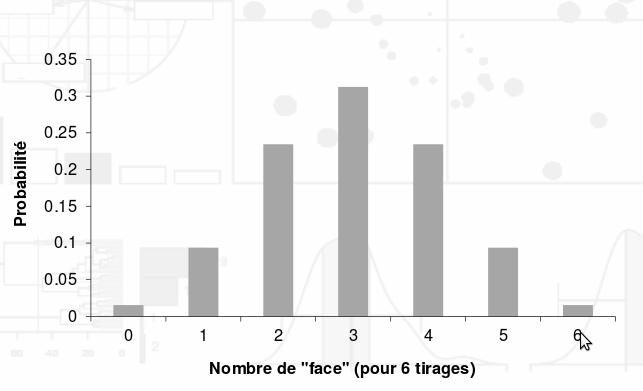
\includegraphics[scale=0.5]{ilu/g1.png}\caption{Probabilit� d'obtention de face entre 0 et 6}\end{center}\end{figure}
ous pouvons voir sur la figure ci dessus, la repr�sentation de la distribution des probabilit�s calcul�es exactement pour chacune des possibilit�s.\newline
il y a plus de probabilit�s d'obtenir 3, exceptionnellement 1 ou 5 et tr�s rarement 0 ou 6.\newline
On peut r�it�rer l'exp�rience sur 20 lanc�s.
\begin{figure}[H]\begin{center}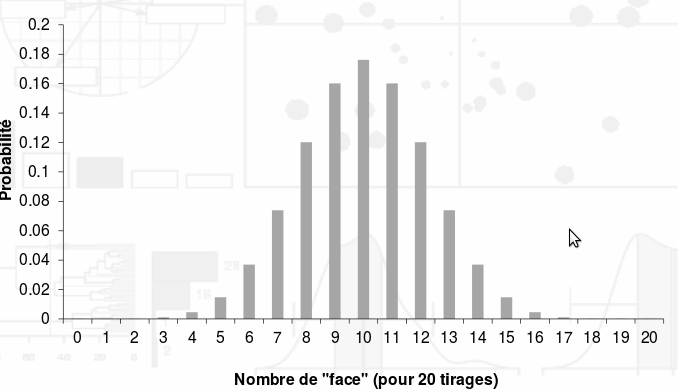
\includegraphics[scale=0.5]{ilu/g2.png}\caption{Probabilit� d'obtention de face entre 0 et 20}\end{center}\end{figure}
il y a plus de probabilit�s d'obtenir 10, exceptionnellement 4 ou 14 et tr�s rarement 2 17.\newline
\\
La distribution de cette Variable al�atoire prend une distribution tr�s r�guli�re et harmonieuse.\newline
Ainsi, quand le nombre de tirage ne tend plus vers 20 mais vers $+\infty$, la loi tend � se rapprocher d'une courbe continue que l'on appelle \textbf{Coubre de Gauss} ou \textbf{Courbe Normale}.

\begin{figure}[H]\begin{center}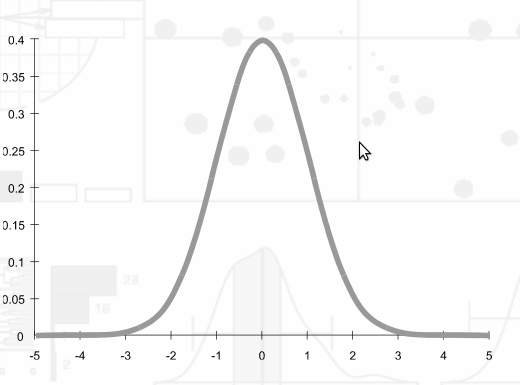
\includegraphics[scale=0.5]{ilu/g3.png}\caption{Repr�sentation de la distribution de la loi Normale}\end{center}\end{figure}
La loi normale a une grande importance en statistique. En effet, quand une variable est la r�sultante d'un grand nombre de variable al�atoires ind�pendante, alors cette variable suit une \textbf{Loi Normale}; Par exemple, la taille d'un individu; elle est la r�sultante de plusieurs facteurs g�n�tiques, environnementaux, sociaux et culturels, \dots L'ensemble de ces facteurs �tant plus ou moins ind�pendants, on peut en conclure que la taille d'un individu suit une loi normale.\newline
\\
Partant de cette constatation, les statisticiens ont d�velopp� des tests optimaux, les plus performants possibles, pour analyser des variables al�atoires suivant des lois Normales.
%%%%%%%%%%%%%%%%%%%%%%%%%%%%%%%%%%%%%%%%%%%%%%%%%%%%%%%%%%%%%%%
%%%%%%%%%%%%%%%%%%%%%%%%%%%%%%%%%%%%%%%%%%%%%%%%%%%%%%%%%%%%%%%
%%%%%%%%%%%%%%%%%%%%%%%%%%%%%%%%%%%%%%%%%%%%%%%%%%%%%%%%%%%%%%%
\chapter{Repr�sentations graphiques}
Nous verrons successivement dans ce cours comment repr�senter les distributions de : 
\begin{itemize}
\item Variables qualitatives
\item Variables quantitatives
\item Diagrammes en b�tons, camemberts, histogrammes, bo�tes � moustaches, diagrammes cart�siens, diagrammes en fagot.
\end{itemize}
Pendant ce cours, nous allons �tudier le fichier \textit{smp1.csv}. Ce fichier est relatif � une �tude sur la sant� mentale en prison r�alis�e en 2004 et financ�e par les minist�res de la justice et de la sant�.\newline
Cette �tude a port�e sur 799 d�tenus masculins, tir�s au sort dans les prisons de France m�tropolitaine.\newline
Dans ce fichier, nous avons un extrait de neuf variables : 
\begin{itemize}	
\item L'Age
\item La Profession du d�tenu 
\item L'existence d'un diagnostic de depression ou schizophr�nie issu du consensus de deux clininciens 
\item Le Niveau de gravit� �ventuelle de la pathologie du d�tenu
\item Le nombre d'enfants du d�tenu 
\end{itemize} 
\textcolor{white}{.}\newline
Ainsi que trois variables relatives � la personnalit� du d�tenu : 
\begin{itemize}
\item Le niveau de recherche de sensation (curiosit�, attrait pour le risque et la nouveaut�) not� \underline{rs}.
\item Le niveau d'�vitement du danger (timidit�, pr�cautionneux) not� \underline{ed}
\item Le niveau de d�pendance � la r�compense (sensibilit� aux relations sociales, influen�able) not� \underline{dr}.
\end{itemize}
\section{Importation des donn�es csv}
Nous allons importer le fichier csv : 
\begin{itemize}
\item \textit{read.csv2("/comptes/E131729J/XX\_Universit�\_fun/univfunR/TP/smp1.csv")} - Fonction d'import
\item \textit{str(smp.c)} - fonction de visulation des donn�es
\end{itemize}

\begin{lstlisting}[language=html]
> smp.c <- read.csv2("/comptes/E131729J/XX_Universit�_fun/univfunR/TP/smp1.csv")
> ### A modifier sous MAC
> str(smp.c)
'data.frame':	799 obs. of  9 variables:
 $ age      : int  31 49 50 47 23 34 24 52 42 45 ...
 $ prof     : Factor w/ 8 levels "agriculteur",..: 3 NA 7 6 8 6 3 2 6 6 ...
 $ dep.cons : int  0 0 0 0 1 0 1 0 1 0 ...
 $ scz.cons : int  0 0 0 0 0 0 0 0 0 0 ...
 $ grav.cons: int  1 2 2 1 2 1 5 1 5 5 ...
 $ n.enfant : int  2 7 2 0 1 3 5 2 1 2 ...
 $ rs       : int  2 2 2 2 2 1 3 2 3 2 ...
 $ ed       : int  1 2 3 2 2 2 3 2 3 2 ...
 $ dr       : int  1 1 2 2 2 1 2 2 1 2 ...
\end{lstlisting}
\section{Variables qualitatives}
\subsection*{Histogramme}
Un fa�on classique de repr�senter la distribution d'une variable al�atoire qualitative est d'utiliser un diagramme en b�tons. Avec \textbf{R}, il faut utiliser les fonctions : 
\begin{itemize}
\item \textit{table} - cette fonction va calculer le nombre de d�tenus ayant chacun des m�tier (en ayant pr�cis� : smp.c\$prof) 
\item \textit{barplot} - cette fonction va repr�senter des b�tons avec pour hauteur, le nombre des d�tenus.
\end{itemize}
\begin{lstlisting}[language=html]
> table(smp.c$prof)
       agriculteur            artisan              autre              cadre 
                 6                 90                 31                 24 
           employe            ouvrier prof.intermediaire        sans emploi 
               135                227                 58                222 
> barplot(table(smp.c$prof))

\end{lstlisting}
\begin{figure}[H]\begin{center}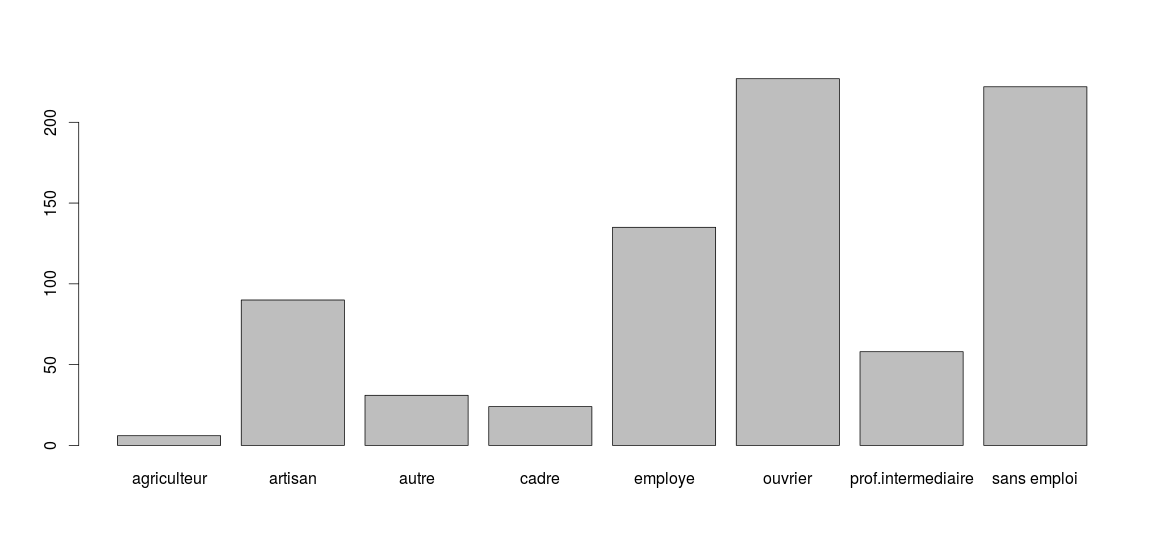
\includegraphics[scale=0.3]{ilu/tp1.png}\caption{Repr�sentation sous forme d'un histogramme}\end{center}\end{figure}
\subsection*{Pie chart}
Un autre grand classique pour repr�senter graphiquement la distribution d'une variable al�atoire cat�gorielle, c'est d'utiliser un camembert (Diagramme circulaire). Avec \textbf{R}, il faut utiliser les fonctions : 
\begin{itemize}
\item \textit{table} - cette fonction va calculer le nombre de d�tenus ayant chacun des m�tier (en ayant pr�cis� : smp.c\$prof) 
\item \textit{pie} - cette fonction va repr�senter des diagrammes circulaires.
\end{itemize}
\textcolor{white}{.}\newline
\textbf{Note : }Certains statisticiens sont r�ticents � l'usage de tel diagrammes. En effet, Il semblerait que l'oeil humain ait des difficult�s � percevoir intuitivement des rapports de surface entre des secteurs de cercle. Alors qu'au contraire, l'oeil humain sertait capable de percevoir intuitivement des hauteurs de b�tons dans un diagramme en b�tons. \newline
\\
En pratique, les repr�sentation en camembert ont une certaine utilit� quand on est int�ress� par la part que repr�sente une profession donn�es par rapport � l'ensemble des d�tenu (sch�ma � transposer en cas �tudi�).  En effet, chaque secteur peut �tre compar� � la superficie totale du disque. \newline
Au contraire, avec un diagramme en b�tons, il faudrait ajouter un b�ton qui repr�sente (par somme), l'ensemble de l'effectif �tudi�, ce qui est tr�s peu commode.
\begin{lstlisting}[language=html]
> table(smp.c$prof)

       agriculteur            artisan              autre              cadre 
                 6                 90                 31                 24 
           employe            ouvrier prof.intermediaire        sans emploi 
               135                227                 58                222 

> pie(table(smp.c$prof))
\end{lstlisting}
\textcolor{white}{.}\newline
\begin{figure}[H]\begin{center}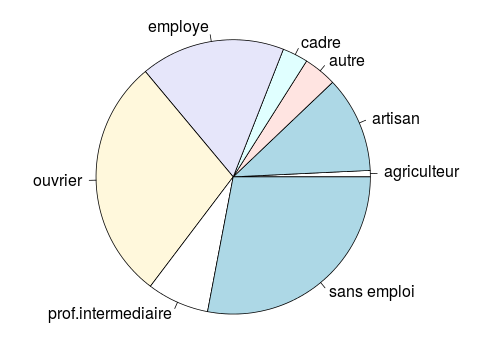
\includegraphics[scale=0.5]{ilu/tp2.png}\caption{Repr�sentation sous forme d'un diagramme circulaire (camembert)}\end{center}\end{figure}
\section{Variables quantitatives}
\subsection*{Histogramme}
Le grand classique pour repr�senter la distribution d'une variable al�atoire quantitative continue est \textbf{l'histogramme}.  \newline
\\
\textbf{Note :} Pour une variable al�atoire continue discr�te, il vaut mieux utiliser un diagramme en b�tons.\newline
La diff�rence entre les deux, c'est qu'avec l'histogramme, les b�tons sont contigus pour bien montrer qu'il y a une continuit� dans les valeurs de la variable. \newline
Le seul point th�orique un peu d�licat avec un histogramme est de savoir comment il faut d�terminer le nombre de b�tons. En pratique, avec \textbf{R}, c'est automatique et cela fonctione tr�s bien 99 fois sur 100.\newline
l'instruction que nous allons utiliser est : 
\textcolor{white}{.}\newline
\begin{itemize}
\item \textit{hist(x)}, avec x, une variable que l'on souhaite repr�senter
\end{itemize}
\begin{lstlisting}[language=html]
> table(smp.c$age)

19 20 21 22 23 24 25 26 27 28 29 30 31 32 33 34 35 36 37 38 39 40 41 42 43 44 
45 46 47 48 49 50 51 15 15 18 13 23 30 22 30 25 21 20 25 18 22 26 20 16 18 25 
24 23 22 23 19 17 19 17 16 12 17 23 16 11 52 53 54 55 56 57 58 59 60 61 62 63 
64 65 66 67 68 69 70 71 72 73 74 77 79 81 83 10  8 11  6 14  9  7  6  7  5  7  
4  5  3  6  4  2  1  1  6  3  2  2  3  1  1  2 
> hist(smp.c$age)
\end{lstlisting}
\begin{figure}[H]\begin{center}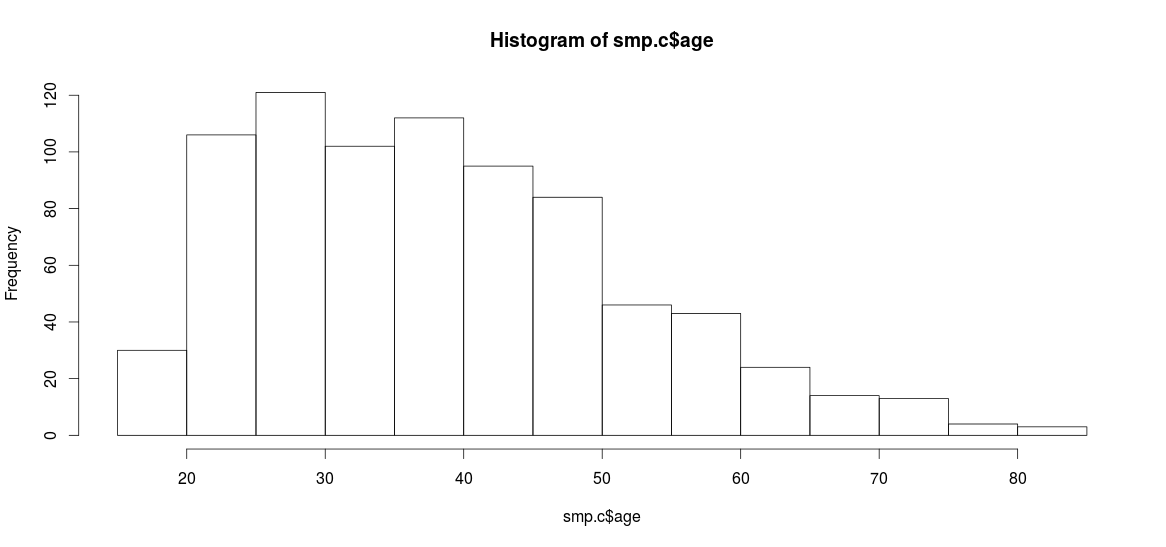
\includegraphics[scale=0.4]{ilu/tp3.png}\caption{Repr�sentation sous forme d'un histogramme}\end{center}\end{figure}
\textbf{Attention : } Pour utiliser la fonction hist(), il faut que les valeurs � repr�senter soient de type num�rique.\newline
\\
On peut �tre un peu dessus de l'aspect graphique et notamment, du fait que les b�tons ne soient pas gris�s. Pour cela, il suffit d'ajouter des instruction � la fonction hist() comment par exemple : \textit{col="grey"}.
\begin{lstlisting}[language=html]
hist(smp.c$age,col="grey")
\end{lstlisting}
\begin{figure}[H]\begin{center}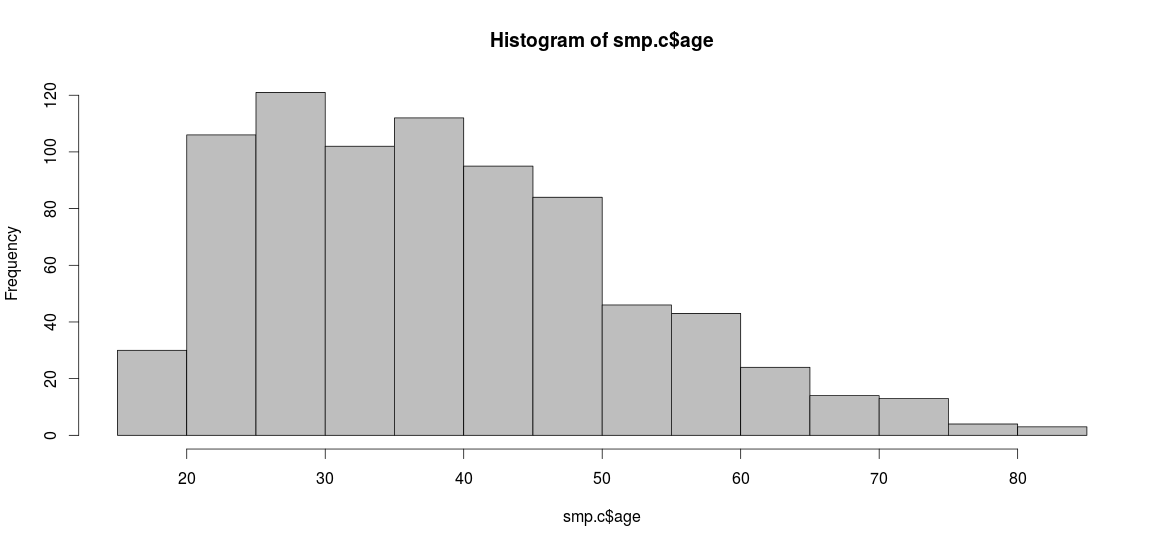
\includegraphics[scale=0.4]{ilu/tp3a.png}\caption{Repr�sentation sous forme d'un histogramme}\end{center}\end{figure}
On peut �galement d�cider de changer le titre du graphique et de changer la l�gende de l'axe des x et des y. 
\begin{lstlisting}[language=html]
hist(smp.c$age,col="grey", main="Repr�sentation des �ges", xlab = "Age",, ylab="Fr�quence")
\end{lstlisting}
\begin{figure}[H]\begin{center}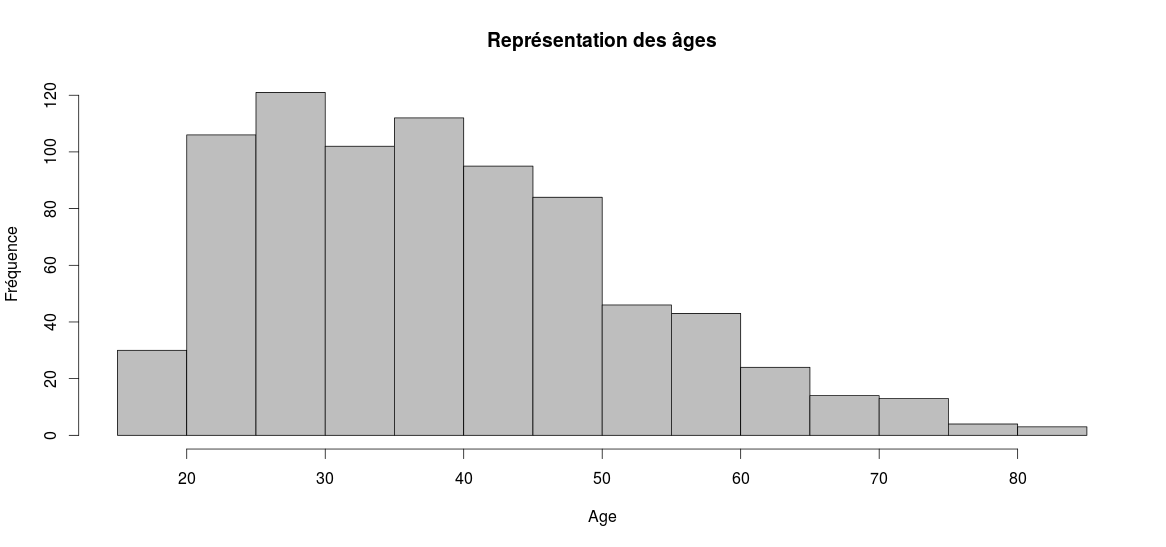
\includegraphics[scale=0.4]{ilu/tp3b.png}\caption{Repr�sentation sous forme d'un histogramme}\end{center}\end{figure}
\textbf{Note : } Pour tout simplement supprimer le titre du graphique, il suffit d'ajouter la fonction \textit{main=""}
\begin{lstlisting}[language=html]
hist(smp.c$age,col="orange", main="", xlab = "Age",, ylab="Fr�quence")
\end{lstlisting}
\textcolor{white}{.}\newline
\subsection*{Bo�te � moustaches - Box plot}
Une solution plus synth�tique est de repr�senter graphiquement la r�partition d'une variable al�atoire quantitative est d'utiliser une \textbf{boite � moustaches} (bo�te de Tukey ou box plot).\newline
L'instruction dans \textbf{R} est : 
\begin{itemize}
\item \textit{boxplot(x)} avec x, une variable que l'on souhaite repr�senter.
\end{itemize}
\textcolor{white}{.}\newline
\textbf{Attention : } Une box plot ne peut repr�senter la distribution que de variables num�riques.

\begin{lstlisting}[language=html]
boxplot(smp.c$age,col="pink", main="", xlab = "Age", ylab="")
\end{lstlisting}
\begin{figure}[H]\begin{center}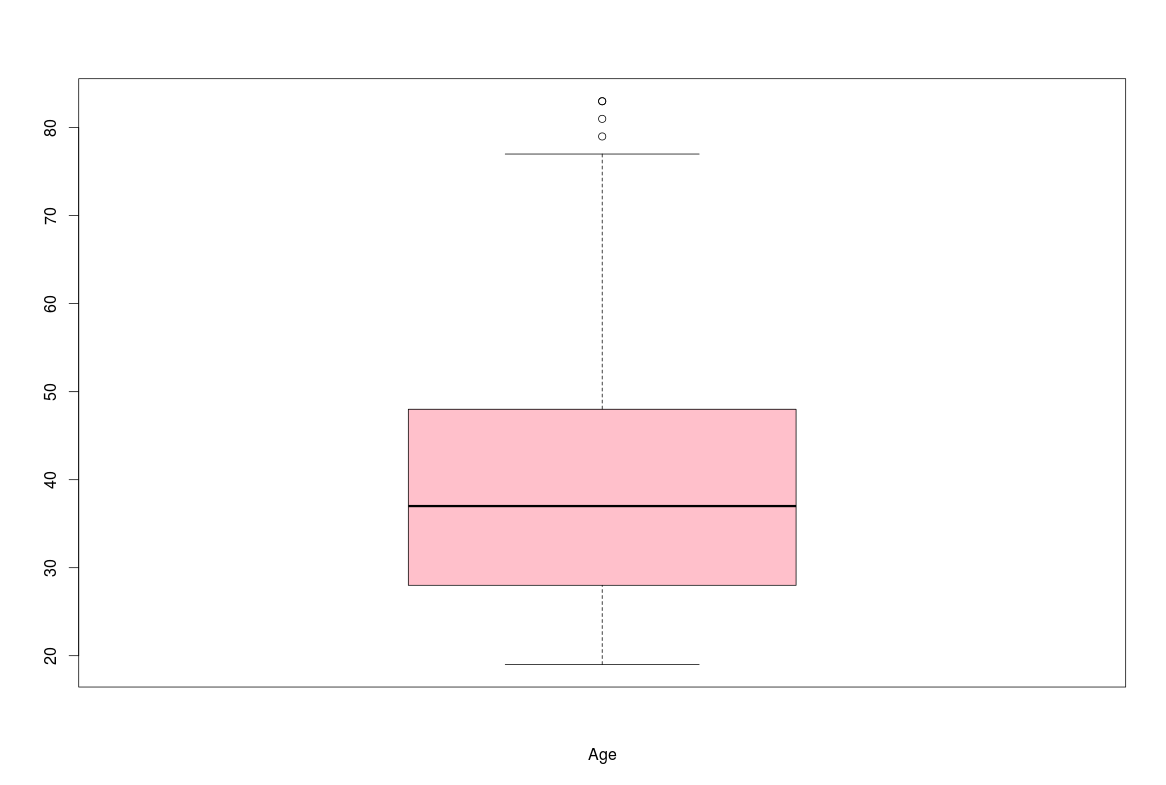
\includegraphics[scale=0.3]{ilu/tp4.png}\caption{Repr�sentation sous forme d'une boite � moustaches}\end{center}\end{figure}
Une bo�te � moustache s'interpr�te de la mani�re suivante : 
\begin{itemize}
\item \textit{A l'int�rtieur de la boite,} vous avez $\sim$ 50\% des donn�es.
\item \textit{Entre le bord sup�rieur de la boite et la moustache sup�rieure,} vous avez $\sim$ 25\% des donn�es.
\item \textit{Entre le bord inf�rieur de la boite et la moustache inf�rieure,} vous avez $\sim$ 25\% des donn�es.
\item les donn�es au dessus et en dessous des moustaches sont appel�es \textit{outlayers} qui sont de donn�es consid�r�es comme aberrantes.
\end{itemize}
La pr�sence des ces outlayers est expliqu� par une impr�cision dans la d�finition des ensembles donn�s ci de�u. \newline
En effet, la moustache sup�rieure correspond :
$$\min(\max, q_{3} + 1.5 (q_{3}-q_{1}))$$
et, la moustache inf�rieure correspond :
$$\max(\min, q_{1} - 1.5 (q_{3}-q_{1}))$$
Les bo�tes � moustaches sont r�ellement utiles pour repr�senter graphiquement la distribution d'une variable quantitative en fonction de sous groupes. Par exemple, on pourrait se demander : \textit{Est ce que la distribution de l'�ge est la m�me selon que l'on ait un niveau de sensation faible, moyen ou �lev� ?}\newline
La r�ponse avec \textbf{R} : 
\begin{lstlisting}[language=html]
> table(smp.c$age)
19 20 21 22 23 24 25 26 27 28 29 30 31 32 33 34 35 36 37 38 39 40 41 42 43 44 
45 46 47 48 15 15 18 13 23 30 22 30 25 21 20 25 18 22 26 20 16 18 25 24 23 22 
23 19 17 19 17 16 12 17 49 50 51 52 53 54 55 56 57 58 59 60 61 62 63 64 65 66 
67 68 69 70 71 72 73 74 77 79 81 83 23 16 11 10  8 11  6 14  9  7  6  7  5  7  
4  5  3  6  4  2  1  1  6  3  2  2  3  1  1  2 

> table(smp.c$rs)
  1   2   3 
249 158 289 
> boxplot(smp.c$age~smp.c$rs,col="pink", main="Corr�lation entre l'�ge et la recherche de sensation ?", xlab = "Recherche de sensation", ylab="Age")
\end{lstlisting}
\begin{figure}[H]\begin{center}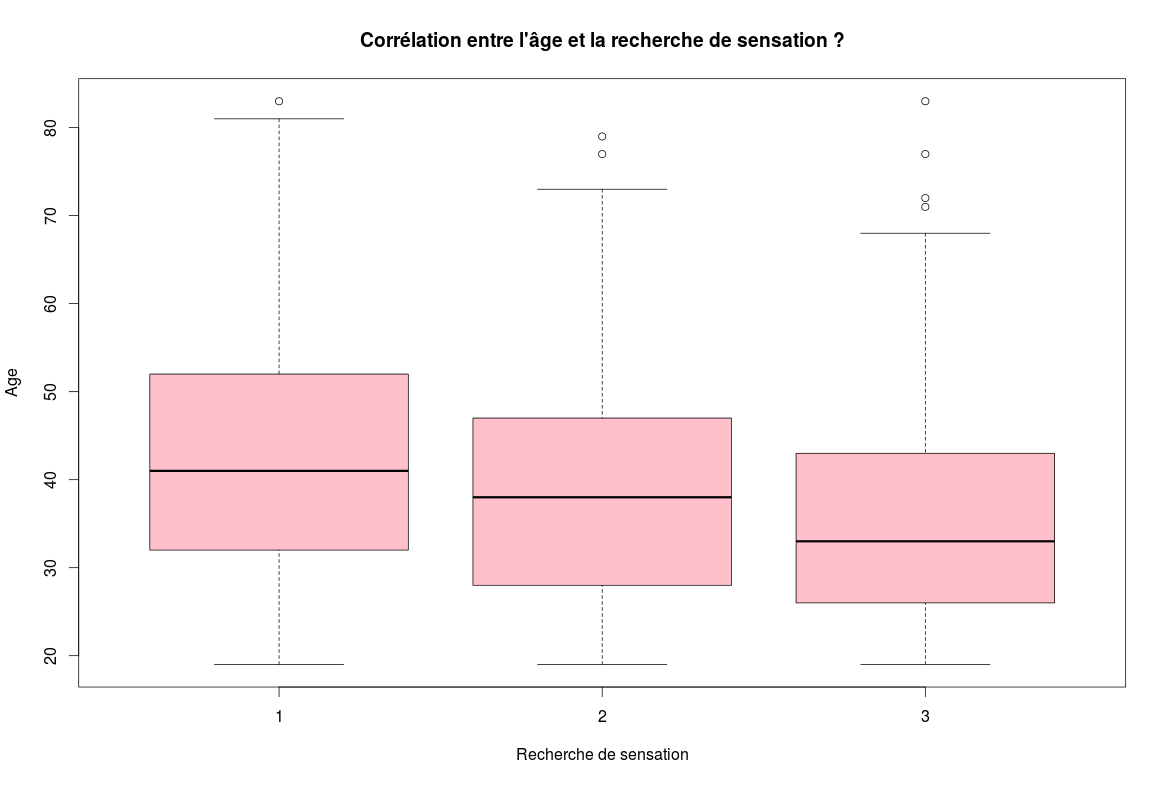
\includegraphics[scale=0.35]{ilu/tp5.png}\caption{Recherche d'influence de l'�ge sur la recherche de sensation}\end{center}\end{figure}
\textit{Analyse :} On observe ici que glolement, la distribution de l'�ge est l�g�rement sup�rieure quand on a un faible niveau de sensation plutot que lorsque l'on a un niveau de sensation �lev�. \newline
\\
Pour repr�senter graphiquement la \underline{distribution conjointe} de deux variables al�atoires quantitatives � l'aide d'un graphique cart�sien, il faut utiliser la fonction : 
\begin{itemize}
\item \textit{plot(x,y)} - avec x et y, respectivement, les varables al�atoires que l'on souhaite repr�senter sur l'axe de x et celui des y.
\end{itemize}
\textcolor{white}{.}\newline
Dans le cas suivant, nous allons repr�senter la distribution de l'�ge et du nombre d'enfants et for logiquement, plus un detenu est �g�, plus il a en moyenne, un nombre d'enfant �lev� :  

\begin{lstlisting}[language=html]
> table(smp.c$age)
19 20 21 22 23 24 25 26 27 28 29 30 31 32 33 34 35 36 37 38 39 40 41 42 43 44 
45 46 47 48 49 50 51 15 15 18 13 23 30 22 30 25 21 20 25 18 22 26 20 16 18 25 
24 23 22 23 19 17 19 17 16 12 17 23 16 11 52 53 54 55 56 57 58 59 60 61 62 63 
64 65 66 67 68 69 70 71 72 73 74 77 79 81 83 10  8 11  6 14  9  7  6  7  5  7  
4  5  3  6  4  2  1  1  6  3  2  2  3  1  1  2 

> table(smp.c$n.enfant)
  0   1   2   3   4   5   6   7   8   9  10  11  13 
214 220 125 101  55  31   7   7   7   2   2   1   1 
> plot(smp.c$age, smp.c$n.enfant,col="blue", main="", xlab = "Age", ylab="Nombre d'enfants")
\end{lstlisting}
\begin{figure}[H]\begin{center}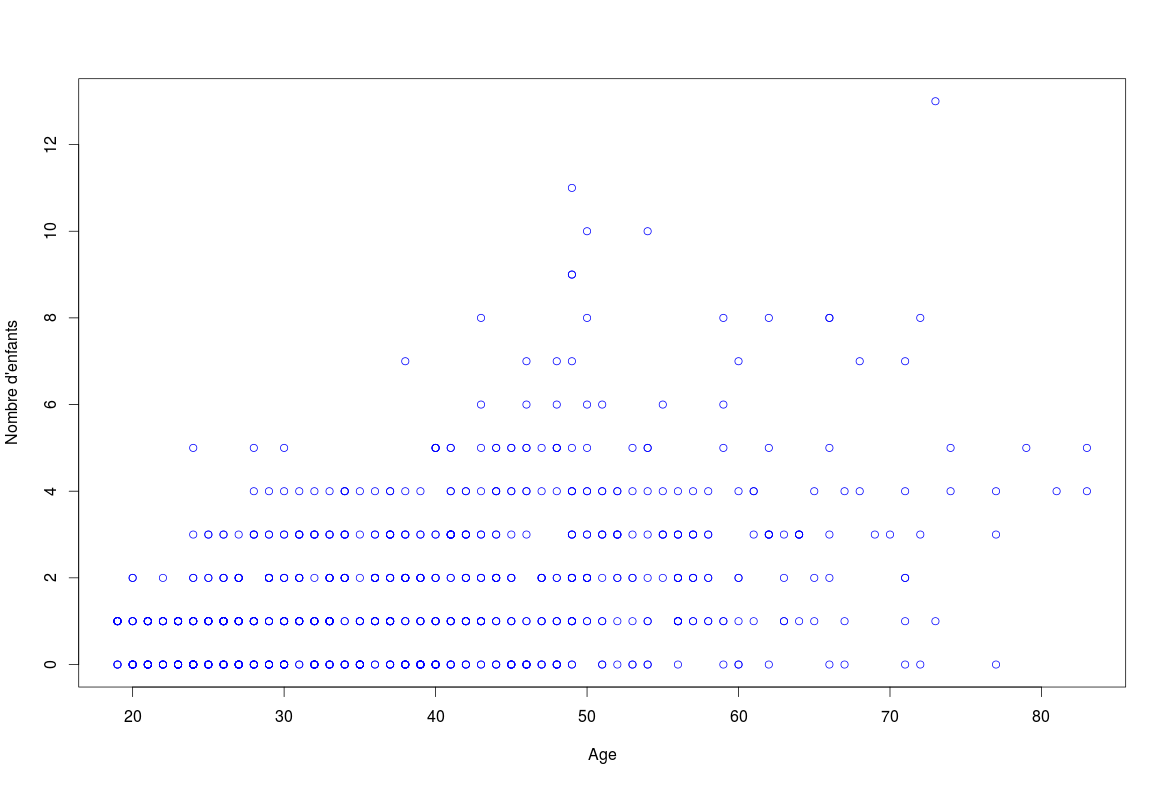
\includegraphics[scale=0.3]{ilu/tp6.png}\caption{Repr�sentation d'une corr�lation entre deux variables al�atoire � l'aide de la fonction plot(x,y)}\end{center}\end{figure}
On peut �tre �tonn� par le fait qu'un semble ne pas y avoir 800 points correspondants au 799 d�tenus et cela s'explique naturellement par le fait que deux d�tenus ayant chacun  50 ans et 2 enfants auront un point situ� exactement au m�me endroit. Ca n'est pas g�nant en soi mais cela peut induire en erreur (on peut avoir l'impression qu'il y a moins de sujets qu'il y en a r�ellement).\newline
Une fa�on de se tirer de ce faux pas est de bouger l�g�rement et de mani�re totalement al�atoire chaque point afin qu'ils se d�collent les uns des autres.\newline
L'instruction correspondante est la fonction \textit{jitter()}.
\begin{lstlisting}[language=html]
plot(jitter(smp.c$age), jitter(smp.c$n.enfant),col="blue", main="", xlab = "Age", ylab="Nombre d'enfants")
\end{lstlisting}
\begin{figure}[H]\begin{center}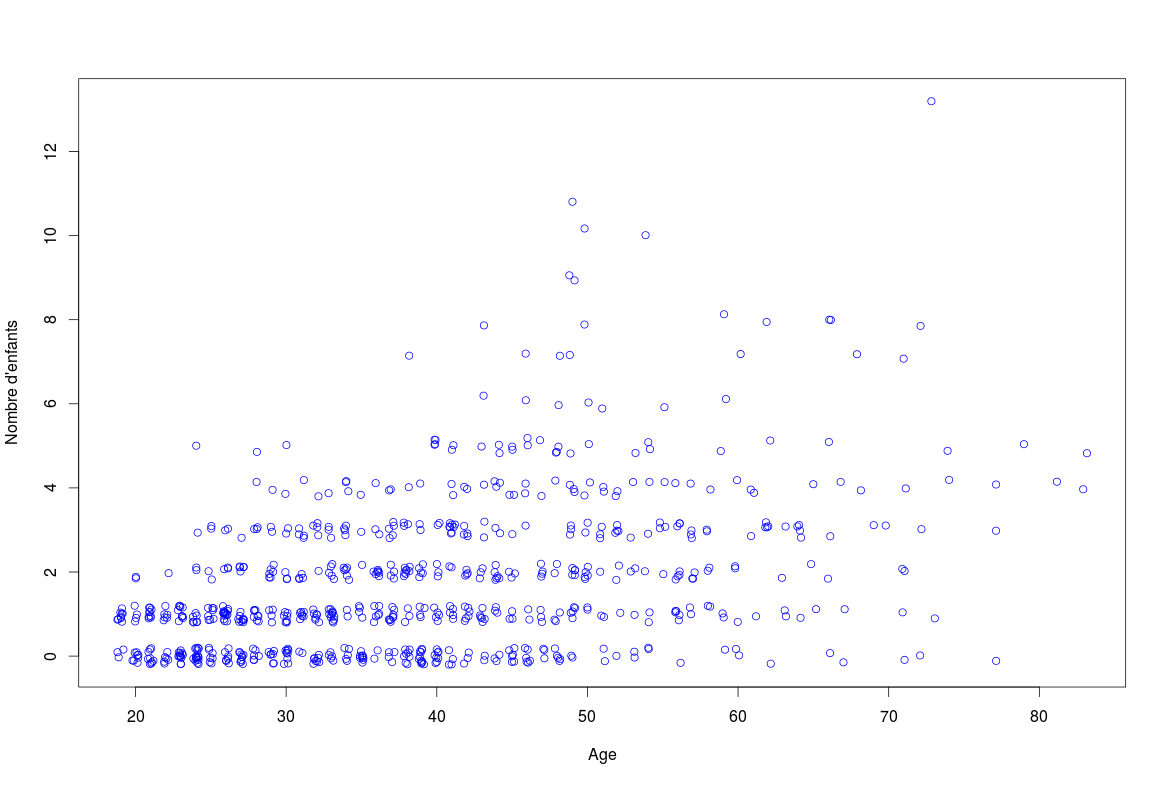
\includegraphics[scale=0.3]{ilu/tp7.png}\caption{Repr�sentation d'une corr�lation entre deux variables al�atoire � l'aide de la fonction plot(x,y) et l'instruction jitter()}\end{center}\end{figure}
D�s lors, nous avons un graphique plus agr�able � regarder o� cette fois, il y a bien 799 points.\newline
\\
Parfois, c'est l'�volution temporelle de la distribution d'une variable al�atoire quantitative que l'on veut repr�senter. Le diagramme correspondant s'appelle un \textbf{diagramme temporel} voire parfois diagramme de temp�rature. Le fichier que nous utilisons concernant la sant� mentale en prison ne nous permet pas de r�aliser des analyses temporelle; En effet, c'est une �tude transversalle ayant �t� men�e en un temps donn�e. Il nous est donc impossible de repr�senter graphiquement l'�volution au cours du temps. \newline
Pour cela, nous allons �tudier un nouveau fichier de donn�es. Cette fois ci, nous allons �tudier des patients d�prim�s, hospitalis�s pour d�pression et qui sont suivis pendant quelques semaines (hdrs.csv).\newline
\\
\begin{lstlisting}[language=html]
> smp.c <- read.csv2("/Users/mehdilatif/Desktop/DIVERS + TEMPLATES/R/TP/outils_hdrs.csv")
> str(smp.c)
'data.frame': 1053 obs. of  3 variables:
 $ NUMERO: int  96 96 96 96 96 96 96 96 157 157 ...
 $ VISIT : int  0 4 7 14 21 28 42 56 0 4 ...
 $ HDRS  : int  34 26 12 7 5 1 1 1 27 19 ...
> summary(smp.c)
     NUMERO           VISIT           HDRS      
 Min.   :  0.00   Min.   : 0.0   Min.   : 0.00  
 1st Qu.: 42.00   1st Qu.: 4.0   1st Qu.: 9.00  
 Median : 94.00   Median :14.0   Median :17.00  
 Mean   : 91.29   Mean   :20.4   Mean   :17.09  
 3rd Qu.:135.00   3rd Qu.:28.0   3rd Qu.:25.00  
 Max.   :191.00   Max.   :56.0   Max.   :44.00  
\end{lstlisting}
\textcolor{white}{.}\newline
L'instruction qui permet de repr�senter graphiquement  l'�volution du score de depression, ici c'est le \textit{hdrs} (Hamilton Depressive Rating Scale) est la fonction \textit{plotmeans()}.\newline
La fonction \textit{plotmeans()} ne fait pas partie du bagage standard \textbf{R} mais de la librairie \textit{gplots}. Pour pouvoir l'utiliser,, il faut d'abord installer le package \textit{gplots}. Il faut donc l'installer comme le pr�sente l'image ci dessous : 
\begin{figure}[H]\begin{center}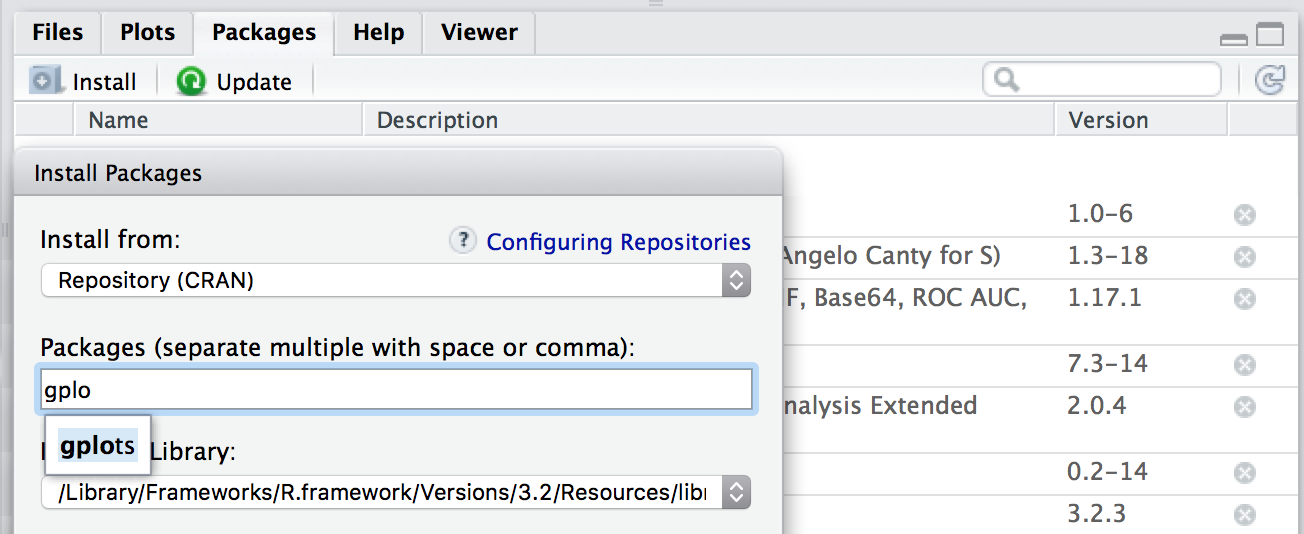
\includegraphics[scale=0.5]{ilu/tp8.png}\caption{Installation du package gplots}\end{center}\end{figure}
L'installation d'un package n'est � re�aliser qu'une seule fois.\newline
\\
Une fois l'installation du package r�alis�e, nous devons faire appel � la librairie de fonction gplots pour pouvoir utiliser la fonction \textit{plotmeans()}. Nous n'avons plus qu'� repr�senter la variable qui nous int�resse (HDRS) en fonction de la variable qui repr�sente le temps (VISIT), les deux s�par�es d'un $\sim$. Les instructions \textit{gap} et \textit{barcol} ne sont l� que pour rendre la repr�sentation graphique plus agr�able � regarder. 
\begin{lstlisting}[language=html]
> library(gplots)
> plotmeans (smp.c$HDRS~smp.c$VISIT,barcol="black",xlab = "Visites", ylab = "Hamilton Rating Depressive Scale")
\end{lstlisting}
\begin{figure}[H]\begin{center}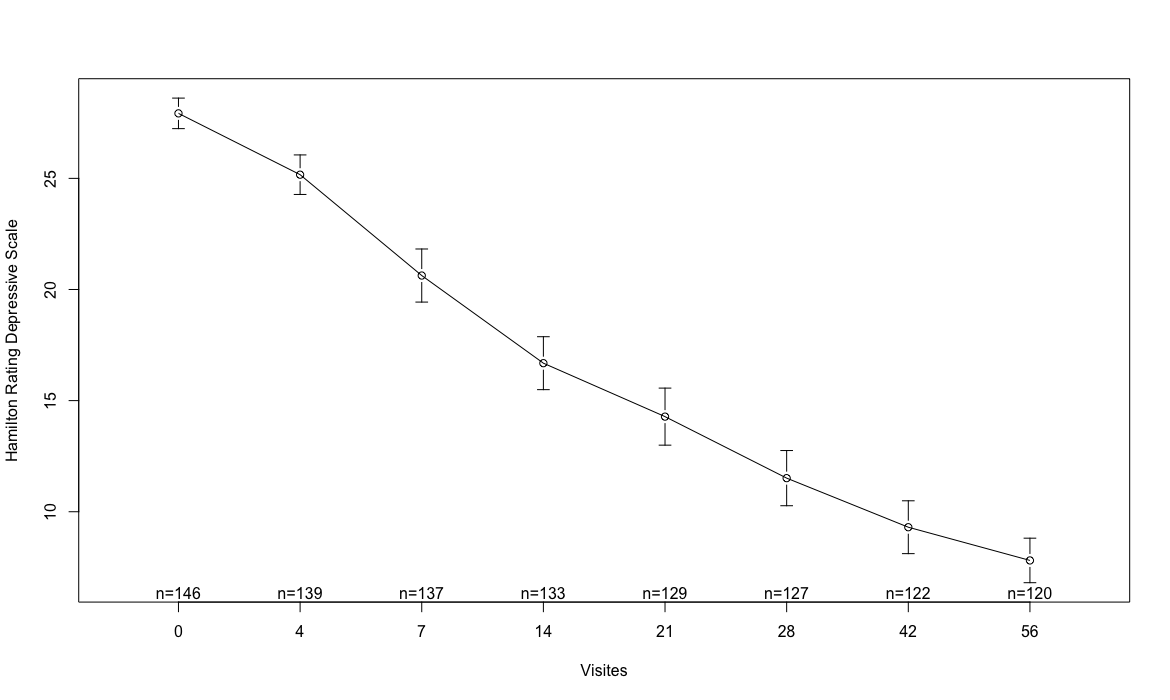
\includegraphics[scale=0.4]{ilu/tp9.png}\caption{Repr�sentation du score HDRS moyen des patients en fonction des visites}\end{center}\end{figure}
Nous pouvons visualiser le fait que l'�tat symptomatique des patients s'am�liore progressivement.\newline
\\
Plut�t que de repr�senter l'�volution moyenne des sujets au cours du temps, il peut �tre int�ressant de repr�senter l'�volution de chaque sujet. Bien s�r, avec plusieurs centaines d'individus dans un jeu de donn�es, l'ensemble peut �tre assez indigeste. N�anmoins, cela donne une impression int�ressante de la variabilit� de l'�volution d'un sujet � l'autre.\newline
La fonction correspondante est la fonction \textit{interaction.plot()}; Sa syntaxe est tr�s simple, il faut : 
\begin{enumerate}
\item D�finir la variable temporelle - dans notre exemple : VISIT
\item D�finir la variable qui repr�sente les sujets - dans notre exemple : NUMERO
\item D�finit la variable qui repr�sente l'information que l'on souhaite repr�senter : dans notre exemple : HDRS
\end{enumerate}
L'instruction \textit{lty=1} correspond au faut que nous voulons des lignes droites continues et \textit{legend} indique la l�gende.
\begin{lstlisting}[language=html]
> interaction.plot(smp.c$VISIT,smp.c$NUMERO,smp.c$HDRS, lty = 1, legend = FALSE)
\end{lstlisting}
\begin{figure}[H]\begin{center}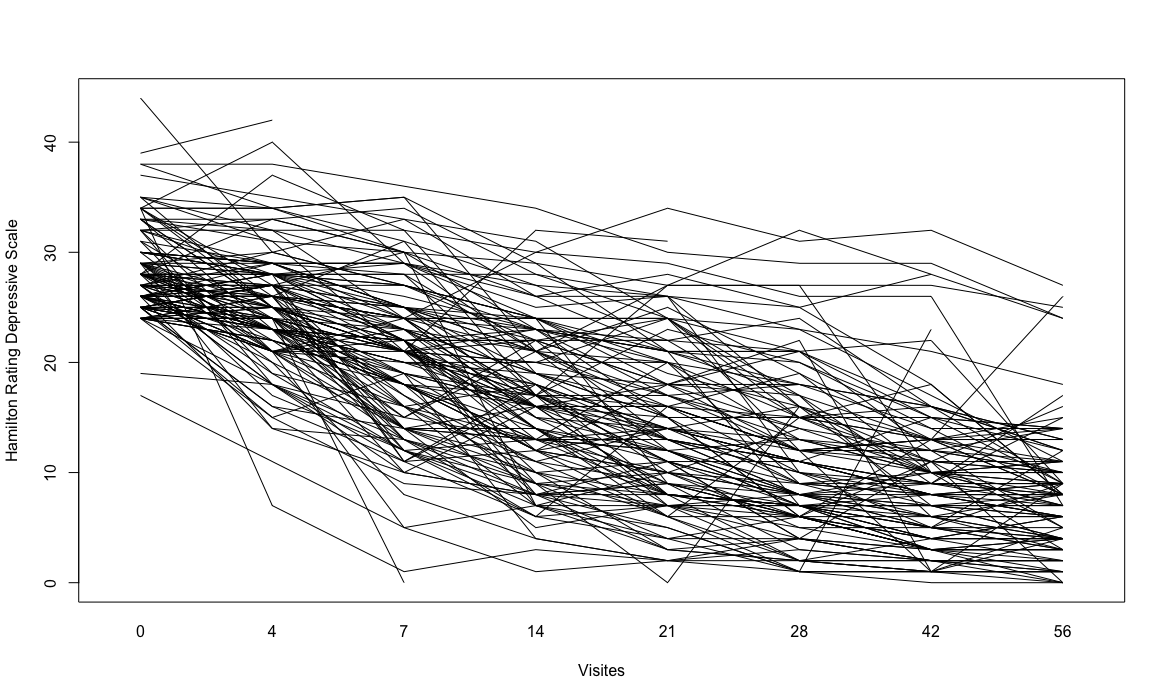
\includegraphics[scale=0.4]{ilu/tp10.png}\caption{Repr�sentation du score HDRS de chaque patient patients en fonction des visites}\end{center}\end{figure}
%%%%%%%%%%%%%%%%%%%%%%%%%%%%%%%%%%%%%%%%%%%%%%%%%%%%%%%%%%%%%%%
%%%%%%%%%%%%%%%%%%%%%%%%%%%%%%%%%%%%%%%%%%%%%%%%%%%%%%%%%%%%%%%
%%%%%%%%%%%%%%%%%%%%%%%%%%%%%%%%%%%%%%%%%%%%%%%%%%%%%%%%%%%%%%%
\chapter{Mesures de position et de dispersion, la th�orie}
Au chapitre pr�c�dent sur les repr�sentations graphiques, nous avons vu qu'un dessin pouvait repr�senter la distribution d'une variable al�atoire, quelle soit qualitative ou quantitative.\newline
Le probl�me, c'est que de nos jours, il n'est pas rare qu'un fichier de donn�es contienne plusieurs centaines voire plusieurs millier de variables al�atoires. Il nous est donc impossible de faire 100 ou 1000 dessins; personne ne les lira, m�me pas l'investigateur.\newline
Nous avons donc besoin de mesures agr�g�es qui synth�tisent l'information et qui la r�sume. De l�, la notion de \textbf{mesures de dispersion et de mesures de position} parmis lesquelles, les tr�s connus \textit{moyennes et �cart types}.\newline
\\
Imaginez que vous ayez � travailler sur une �tude visant � �valuer la consommation de Cannabis en France, selon que la population se situe autour d'un age de 15 ans ou 60 ans, la probl�matique de sant� publique sous jacente, les d�terminants de consommation vont �tre compl�tement diff�rents. Il est donc indispensable de disposer d'un param�tre simple qui permet de dire imm�diatement autoir de quel �ge se situe la population. On appelle �a une mesure de position.\newline
En compl�ment de cette mesure de position, on a besoin de connaitre la dispersion; Si vous prenez des adolescents et que vous les interrogez en classe de troisi�me, ils auront tous autour de 15 ans. Cependant, si vous interrogez en m�langeant coll�ge et lyc�e, vous aurez des jeunes dont l'�ge varie entre 11 et 18 ans, la probl�matique sera compl�tement diff�rente.\newline
\\
Nous allons donc voir dans ce chapitre, des mesures de positions et de dispersions. Pour le cas de variables cat�gorielles, les mesures de positions sont assez simples � mettre en place, il suffit de lister les pourcentage de toute les modalit�s de cat�gories de la variable qualitative ou cat�gorielle �valu�e.\newline
Pour une variable quantitative, c'est un petit peu plus compliqu� et vous savez qu'il existe deux param�tres, la moyenne et la m�diane.\newline
En ce qui concerne les mesures de dispersion, on utilise les notion de quartiles et d'ecart- type (Ce dernier, tr�s connu mais pas forc�ment facile � utiliser car son interpr�tation est d�licate). 
\section{Mesures de position}
\subsection{Moyenne et m�diane}

\begin{figure}[H]\begin{center}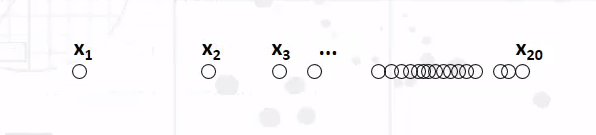
\includegraphics[scale=0.5]{ilu/g4.png}\end{center}\end{figure}
Consid�rons donc une variable avec une vingtaine d'observations. L'objectif est de trouver une valeur autour de laquel se situe globalement l'ensemble des observations. \newline
\\ La premi�re solution, la plus classique, serait de calculer la \textbf{moyenne}, c'est � dire faire : 
$$\frac{1}{\textrm{nombre d'Observation}}\sum_{i=1}^{i=20} x_{i}$$
On est conditionn� depuis l'�cole primaire � avoir la moyenne de nos r�sultats qu'elle soit pond�r�e ou non.  Bref, dans la vie de tous les jours, on utilise des moyennes et on ne se rend m�me plus compte qu'en r�alit�, le \underline{sens � donner au moyenne n'est pas si �vident que �a}.\newline 
\\
\textbf{Exemple :} Vous avez eu 15 notes et la moyenne de ces 15 notes et 12, Qu'est ce que cela signifie ?\newline
Il est impossible de savoir si il y a plus de notes sup�rieures � 12 que de notes inf�rieures � 12 ou le contraire.\newline
\\
Un fa�on de se repr�senter g�om�triquement la moyenne est de consid�rer qu'elle est le barycentre de l'ensemble des observations. La moyenne ainsi un sens physique. \newline
Elle n'est pas le seul param�tre que l'on peut utiliser.\newline
\\
Il existe aussi la \textbf{m�diane}. La m�diane a un sens beaucoup plus clair : \textit{50\% des observations lui sont plus petites et 50\% des observations lui sont plus grandes.}\newline
\begin{figure}[H]\begin{center}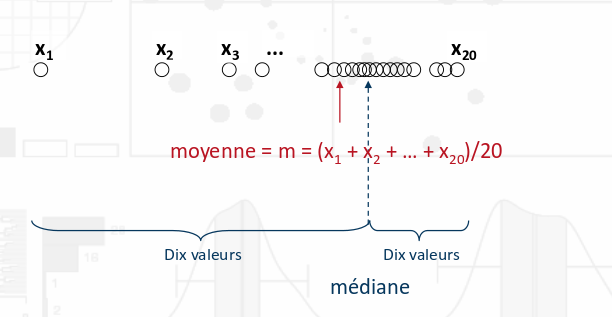
\includegraphics[scale=0.5]{ilu/g5.png}\end{center}\end{figure}
Si la \textbf{distribution est sym�trique}, alors la m�diane est �gale � la moyenne. Sinon, et c'est la situation pr�sente dans le graphique pr�sent� ci dessus o� l'onvoit que les observations sont beaucoup plus dispers�es � gauche qu'� droite, alors il y a des diff�rences non n�gligeables entre la moyenne et la m�diane.\newline
\\
Mais en pratique, est il plus int�ressant d'utiliser des m�dianes ou des moyennes ?\newline
\subsection*{Avantages et inconv�nients}

\paragraph*{La m�diane :} La m�diane poss�de tout d'abord un c�t� \textbf{intuitif}; Au moins, nous savons ce que cela signifie (50 \% des valeurs plus grandes et 50\% des valeurs plus petites). \newline
On peut �galement parler de la \textbf{robustesse} de cette mesure. En effet, la m�diane est tr�s peu sensible au valeurs extr�mes. Sur un jeu de donn�es contenant 50 sujets dont on analyse l'�ge, si il y � une erreur de saisie (25 ans devient 2500 ans), alors la m�diane ne va pas changer puisque cette derni�re coupe juste l'�chantillon en deux. Que les valeurs extr�mes soient hyper extr�mes ou peu extr�mes, cela ne changera rien � la m�diane alors que �a impactera fortement la moyenne. \newline
La m�diane est donc un param�tre robuste.
\paragraph*{La moyenne : } Tout d'abord, ce param�tre est \textbf{simple a calculer} (somme des observations sur nombre d'observation) alors que la m�diane n'est pas du tout aussi simple. En effet, avant de calculer une m�diane, il faut au pr�alable, avoir class� l'ensemble des observations dans une ordre d�finit ou naturel.\newline
De plus, la moyenne poss�de une propri�t� g�om�trique et physique; c'est le \textbf{barycentre ou le centre de gravit�} de la distribution.\newline
Autant la m�diane n'est pas un "beau" param�tre en termes math�matiques, la moyenne a des propri�t�s math�matiques int�ressantes.	\newline
Au del� des propri�t�s math�matiques, la moyenne � un \textbf{int�r�t comptable} . On dit traditionnellement que pour repr�senter une variable qui a une distribution asym�trique ou assez fortement asym�trique, il faudrait utiliser une m�diane et non une moyenne; et bien ce n'est pas toujours vrai. Prenons pour exemple la distribution de la dur�e de s�jour de patients hospitalis�s. On suppose que les patients vont �tre hospitalis�s seulement quelques jours et puis, quelques-uns d'entre eux vont rester, � cause de complications, plusieurs semaines, voire plusieurs mois, mais ils sont tr�s rares. Il serait logique donc, pour essayer d'avoir un param�tre de position de la dur�e de s�jour d'avoir la m�diane. Or les directeurs d?h�pitaux s'int�ressent � la dur�e moyenne de s�jour. En effet, si vous avez la dur�e moyenne de s�jour et que vous connaissez le nombre de s�jours hospitaliers annuels. quand vous multipliez l'un par l'autre, vous avez directement le nombre de jour de lits de lits d'hospitalisation occup�s dans l'ann�e et si l?h�pital est pay� qu'au nombre de jours de lits d'hospitalisation occup�s, alors le directeur d'h�pital sait exactement combien il va gagner sur son ann�e.
\section{Mesures de dispersion}
Analysons maintenant les param�tres de dispersion. \newline
Nous consid�rons toujours les 20 observations de notre variable al�atoire
et dans un premier temps, nous nous int�resser � l'intervalle inter quartile.
\begin{figure}[H]\begin{center}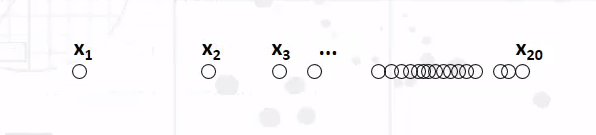
\includegraphics[scale=0.5]{ilu/g4.png}\end{center}\end{figure}
\subsection{Quartiles, �cart-type}
La m�diane d�coupait le jeu d'observartions en deux parts �gales alors que les \textbf{Quartiles} d�coupent ce m�me jeu d'observations en quatres parts �gales.
\begin{figure}[H]\begin{center}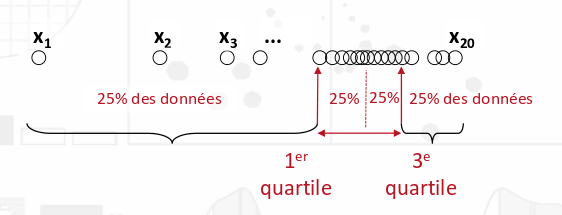
\includegraphics[scale=0.5]{ilu/g6.png}\end{center}\end{figure}
Il y a 25\% des sujets qui sont inf�rieurs au premier quartile ($q_{1}$),  25\% des sujets qui sont superieurs au troisi�me quartile ($q_{3}$) et donc entre $q_{1}$ et $q_{3}$, \textbf{l'espace interquartile}, nous avons 50\% des observations; ce sont les 50\% qui se regroupent autours de la m�diane. \textbf{l'intervalle interquartile} a ainsi un sens clair et imm�diat : \textbf{il regroupe la moiti� de l'�chantillon qui se situe autour de la m�diane}. On se rappelle des boites � moustaches : 
\begin{figure}[H]\begin{center}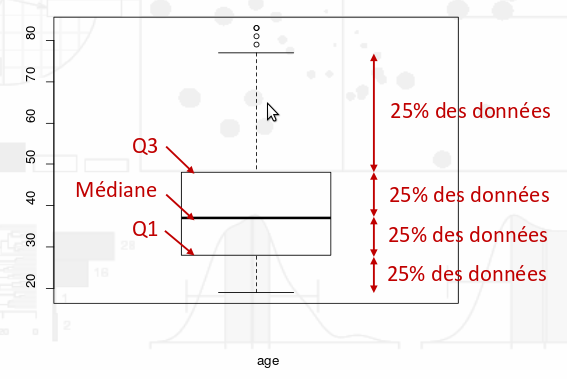
\includegraphics[scale=0.5]{ilu/g7.png}\end{center}\end{figure}
L'intervalle interquartile n'est pas le param�tre de dispersion le plus utilis�. On pr�f�re en effet utiliser l'�cart-type.\newline 
Par d�finition l'�cart-type se calcule de la mani�re suivante :
$$\sigma^{2} = \textrm{Var} = \frac{1}{n} \sum_{x_{i} -\bar{x}}$$
$$\sigma = \sqrt{ \frac{1}{n} \sum_{x_{i} -\bar{x}}}$$
En pratique, cela ne veut rien dire \dots.
L'�cart-type n'a aucun sens intuitif alors pourquoi utiliser un tel param�tre ? \newline
\\
Une premi�re explication, c'est qu'� l'instar de la moyenne, l?�cart-type � une certaine interpr�tation physique : il correspond � l?inertie. De la m�me fa�on l'�cart-type a d'excellentes propri�t�s math�matiques (on le retrouve dans beaucoup de tests statistiques). Ce dernier �tant �galement totalement diff�rent de l'espace inter quartile qui, comme la m�diane, n'a pas du tout de bonnes propri�t�s math�matiques.\newline
Enfin, l'�cart-type poss�de une propri�t� qui le rend tr�s utile et tr�s simple � calculer : l'�cart-type au carr�, c'est � dire la variance, correspond � la moyenne des carr�s moins la moyenne au carr� :
$$\sigma^{2} = \frac{(x_{1}+ \dots +x_{20})^{2}}{20} - (\frac{x_{1}+ \dots +x_{20}}{20})^{2}$$
Nous allons voir qu'au d�but du $XX^{e}$ si�cle, cette propri�t� fantastique.\newline 
\paragraph{Comment calculer la variance :}
Calcul de la variance \textbf{Old School}
\begin{center}

\begin{tabular}{lllllll}
\cline{1-4}
\multicolumn{1}{|l|}{$x_{i}$} & \multicolumn{1}{l|}{$\sum x_{i}$} & \multicolumn{1}{l|}{$x_{i}^{2}$} & \multicolumn{1}{l|}{$\sum x_{i}^{2}$} &  &  &  \\ \cline{1-4}
$x_{1}$                       & $s_{1}$                           & $x_{1}^{2}$                      & $q_{1}$                               &  &  &  \\
$x_{2}$                       & $s_{2}$                           & $x_{2}^{2}$                      & $q_{2}$                               &  &  &  \\
\dots                         & \dots                             & \dots                            & \dots                                 &  &  &  \\
$x_{1000}$                    & $s_{1000}$                        & $x_{1000}^{2}$                   & $q_{1000}$                            &  &  &  \\
                              &                                   &                                  &                                       &  &  & 
\end{tabular}
\end{center}
Avec $$s_{2} = \sum_{i=1}^{2} x_{i} = x_{1} + x_{2}= s_{1}+s_{2} $$
Et $$q_{2} = \sum_{i=1}^{2} x_{i}^{2} = x_{1}^{2} + x_{2}^{2} = q_{1}+q_{2}$$
\textit{Principe de la somme cumulative}\newline
\\
Le calcul de la variance s'effectue donc de la mani�re suivante : 
$$\textrm{Var} = \frac{q_{1000}}{1000} - (\frac{s_{1000}}{1000})^{2}$$
$$\sigma = \sqrt{\textrm{Var}} = \sqrt{\frac{q_{1000}}{1000} - (\frac{s_{1000}}{1000})^{2}}$$
Cette formule permet donc de simplifier le calcul de la variance mais �galement de l'�cart-type puisque l'on a qu'une racine carr� � calculer (� l'�poque, ils n'avaient pas de calculatrice).\newline
\\ 
Imaginons qu'apr�s le calcul termin�, on se rend compte qu'il manque une valeur, \textbf{NO PANIC} : 

\begin{center}
\begin{tabular}{lllllll}
\cline{1-4}
\multicolumn{1}{|l|}{$x_{i}$} & \multicolumn{1}{l|}{$\sum x_{i}$} & \multicolumn{1}{l|}{$x_{i}^{2}$} & \multicolumn{1}{l|}{$\sum x_{i}^{2}$} &  &  &  \\ \cline{1-4}
$x_{1}$                       & $s_{1}$                           & $x_{1}^{2}$                      & $q_{1}$                               &  &  &  \\
$x_{2}$                       & $s_{2}$                           & $x_{2}^{2}$                      & $q_{2}$                               &  &  &  \\
\dots                         & \dots                             & \dots                            & \dots                                 &  &  &  \\
$x_{1000}$                    & $s_{1000}$                        & $x_{1000}^{2}$                   & $q_{1000}$                            &  &  &  \\
\textcolor{red}{$x_{1001}$}                    & \textcolor{red}{$s_{1001}$ }                      & \textcolor{red}{$x_{1001}^{2}$}                  & \textcolor{red}{$q_{1001}$}                          &  &  &
\end{tabular}
\end{center}

$$\textrm(Var) = \frac{q_{1000}+x_{1001}^{2}}{1001} - (\frac{s_{1000}+x_{1001}}{1001})^{2}$$
$$\sigma = \sqrt{\textrm{Var}} = \sqrt{\frac{q_{1000}+x_{1001}^{2}}{1001} - (\frac{s_{1000}+x_{1001}}{1001})^{2}}$$
\subsection*{Que penser d'un �cart-type}
Au total, l'�cart-type est principalement utilis� pour ses propri�t�s math�matiques et calculatoires mais pas dans le sens qu'on pourrait intuitivement lui donner.\newline
En effet, l'�cart type est utilis� dans le calcul suivant :\newline
\\
\textit{Si la variable � une distribution normale, l'intervalle qui contient $[\bar{x}-\sigma, \bar{x}+\sigma]$ repr�sente approximativement les $2/3$ des donn�es (c'est � dire la majorit� des donn�es de la distribution)}.
%%%%%%%%%%%%%%%%%%%%%%%%%%%%%%%%%%%%%%%%%%%%%%%%%%%%%%%%%%%%%%%
%%%%%%%%%%%%%%%%%%%%%%%%%%%%%%%%%%%%%%%%%%%%%%%%%%%%%%%%%%%%%%%
%%%%%%%%%%%%%%%%%%%%%%%%%%%%%%%%%%%%%%%%%%%%%%%%%%%%%%%%%%%%%%%
\chapter{Mesures de position et de dispersion, la pratique}
Pour calculer tous ces param�tres dans \textbf{R}, il suffit d'utiliser la fonction \textit{summary}. Le logiciel va automatiquement retourner : 
\begin{itemize}
\item Pour les variables qualitatives
\begin{itemize}
\item le minimum,
\item le 1 er quartile,
\item la m�diane,
\item la moyenne,
\item le 3 �me quartile,
\item le maximum
\item le nombre de donn�es manquantes, il est tr�s important de conna�tre le nombre de donn�es manquantes pour chaque variable.
\end{itemize}
\item Pour les variables cat�gorielles

\begin{itemize}
\item le nombre de sujets pour chaque modalit�
\item les donn�es manquantes
\end{itemize}
\end{itemize}
\begin{lstlisting}[language=html]
> smp.c <- read.csv2("/Users/mehdilatif/Desktop/DIVERS + TEMPLATES/R/TP/outils_hdrs.csv")
> str(smp.c)
'data.frame':	799 obs. of  9 variables:
 $ age      : int  31 49 50 47 23 34 24 52 42 45 ...
 $ prof     : Factor w/ 8 levels "agriculteur",..: 3 NA 7 6 8 6 3 2 6 6 ...
 $ dep.cons : int  0 0 0 0 1 0 1 0 1 0 ...
 $ scz.cons : int  0 0 0 0 0 0 0 0 0 0 ...
 $ grav.cons: int  1 2 2 1 2 1 5 1 5 5 ...
 $ n.enfant : int  2 7 2 0 1 3 5 2 1 2 ...
 $ rs       : int  2 2 2 2 2 1 3 2 3 2 ...
 $ ed       : int  1 2 3 2 2 2 3 2 3 2 ...
 $ dr       : int  1 1 2 2 2 1 2 2 1 2 ...
> summary(smp.c)
      age                       prof        dep.cons         scz.cons        grav.cons    
 Min.   :19.0   ouvrier           :227   Min.   :0.0000   Min.   :0.0000   Min.   :1.000  
 1st Qu.:28.0   sans emploi       :222   1st Qu.:0.0000   1st Qu.:0.0000   1st Qu.:2.000  
 Median :37.0   employe           :135   Median :0.0000   Median :0.0000   Median :4.000  
 Mean   :38.9   artisan           : 90   Mean   :0.3967   Mean   :0.0826   Mean   :3.643  
 3rd Qu.:48.0   prof.intermediaire: 58   3rd Qu.:1.0000   3rd Qu.:0.0000   3rd Qu.:5.000  
 Max.   :83.0   (Other)           : 61   Max.   :1.0000   Max.   :1.0000   Max.   :7.000  
 NA's   :2      NA's              :  6                                     NA's   :4      
    n.enfant            rs              ed              dr       
 Min.   : 0.000   Min.   :1.000   Min.   :1.000   Min.   :1.000  
 1st Qu.: 0.000   1st Qu.:1.000   1st Qu.:1.000   1st Qu.:1.000  
 Median : 1.000   Median :2.000   Median :2.000   Median :2.000  
 Mean   : 1.755   Mean   :2.057   Mean   :1.866   Mean   :2.153  
 3rd Qu.: 3.000   3rd Qu.:3.000   3rd Qu.:3.000   3rd Qu.:3.000  
 Max.   :13.000   Max.   :3.000   Max.   :3.000   Max.   :3.000  
 NA's   :26       NA's   :103     NA's   :107     NA's   :111    
> 
\end{lstlisting}
Il existe �galement une autre fonction qui permet de r�sumer l'ensemble des informations concernant des variables al�atoires de mani�re plus claire: la fonction \textbf{describe()} qui se trouve dans le package \textit{prettyR}
\begin{lstlisting}[language=html]
> setwd("~/XX_Universit�_fun/univfunR/TP")
> outil <-read.csv2("/comptes/E131729J/XX_Universit�_fun/univfunR/TP/outils_hdrs.csv")
> str(outil)
'data.frame':	1053 obs. of  3 variables:
 $ NUMERO: int  96 96 96 96 96 96 96 96 157 157 ...
 $ VISIT : int  0 4 7 14 21 28 42 56 0 4 ...
 $ HDRS  : int  34 26 12 7 5 1 1 1 27 19 ...
> summary(outil)
     NUMERO           VISIT           HDRS      
 Min.   :  0.00   Min.   : 0.0   Min.   : 0.00  
 1st Qu.: 42.00   1st Qu.: 4.0   1st Qu.: 9.00  
 Median : 94.00   Median :14.0   Median :17.00  
 Mean   : 91.29   Mean   :20.4   Mean   :17.09  
 3rd Qu.:135.00   3rd Qu.:28.0   3rd Qu.:25.00  
 Max.   :191.00   Max.   :56.0   Max.   :44.00  
> library(prettyR)
> describe(outil)
Description of outil 

 Numeric 
        mean median     var    sd valid.n
NUMERO 91.29     94 2780.79 52.73    1053
VISIT  20.40     14  327.55 18.10    1053
HDRS   17.09     17   87.90  9.38    1053
\end{lstlisting}
La fonction \textbf{describe()} �tant tr�s int�ressante, elle ne pr�sente n�anmoins ni les quartiles, ni les maximum et minimum; donn�es absolument indispensables car lorsque vous pr�senterez un fichier, les valeurs minimales et maximales vous permettrons de d�tecter les donn�es ab�rantes. Par exemple, si vous avez la variable \textit{smp\$age} et que vous d�tectez une erreur de mesure \textbf{e.g} max = 1596 ans.\newline
\textbf{Cependant,} on peut demander � la fonction \textbf{describe()} d'effectuer d'autres calculs que ceux propos�s de base. Par exemple ,nous allons demander � la fonction de calculer les param�tres suivants : 
\begin{itemize}
\item moyenne
\item �cart-type
\item variance
\item la m�diane
\item le minimum
\item le maximum
\item le nombre de sujets dans l'�chantillon
\end{itemize}
\begin{lstlisting}[language=html]
> library(prettyR) #Describe
> describe(outil, num.desc =c("mean","sd","var","median","min","max","valid.n"))
Description of outil 

 Numeric 
        mean    sd     var median min max valid.n
NUMERO 91.29 52.73 2780.79     94   0 191    1053
VISIT  20.40 18.10  327.55     14   0  56    1053
HDRS   17.09  9.38   87.90     17   0  44    1053
\end{lstlisting}
Il est possible de demander � la fonction de retourner les valeurs des quantiles pour n'importe quelle valeur de ce dernier.\newline
Comme nous l'avons vu en CM, il est possible �galement d'afficher le skewness repr�sentant le coefficient de dissym�trie et le kurtosis repr�sentant le coefficient d'aplatissement.
\begin{lstlisting}[language=html]
> library(prettyR) #Describe
> library(moments) #pour skewness et kurtosis
> describe(outil, num.desc =c("mean","sd","var","median","min","max","valid.n","skewness","kurtosis","q25","q75"))
Description of outil 

 Numeric 
        mean    sd     var median min max valid.n skewness kurtosis q25
NUMERO 91.29 52.73 2780.79     94   0 191    1053     0.07     1.81  42
VISIT  20.40 18.10  327.55     14   0  56    1053     0.72     2.30   4
HDRS   17.09  9.38   87.90     17   0  44    1053     0.06     1.98   9
       q75
NUMERO 135
VISIT   28
HDRS    25
\end{lstlisting}
Il est parfois tr�s utile de calculer simplement les valeurs de la moyenne ou de l'�cart type. Il existe des fonctions permettant de retourner ces valeurs : 
\textbf{mean()} pour la moyenne et \textbf{sd()} pour l'�cart type. Il en est de m�me pour les fonctions de bases type min, max, cov, \dots Elle seront pr�sent�es plus en d�tail dans le TP de Probabilit�s discr�tes.\newline
\\
Et pour une variable cat�gorielle, si vous voulez conna�tre les modalit�s, vous pouvez utiliser la fonction table(). La fonction table() est ici utilis�e avec les options \textit{deparse.level=2}. �a permet d'avoir le nom de la variable affich� et puis useNA qui est utilis� ici pour pouvoir savoir combien de sujets ont eu des donn�es manquantes pour leurs professions
\begin{lstlisting}[language=html]
> smp <-read.csv2("/comptes/E131729J/XX_Universit�_fun/univfunR/TP/smp1.csv")
> mean(smp$age)
[1] NA
> mean(smp$age, na.rm = TRUE)
[1] 38.89962
> sd(smp$age)
[1] NA
> sd(smp$age, na.rm = TRUE)
[1] 13.28098
> table(smp$prof, deparse.level = 2, useNA = "always")
smp$prof
       agriculteur            artisan              autre 
                 6                 90                 31 
             cadre            employe            ouvrier 
                24                135                227 
prof.intermediaire        sans emploi               <NA> 
                58                222                  6 
\end{lstlisting}
%%%%%%%%%%%%%%%%%%%%%%%%%%%%%%%%%%%%%%%%%%%%%%%%%%%%%%%%%%%%%%%
%%%%%%%%%%%%%%%%%%%%%%%%%%%%%%%%%%%%%%%%%%%%%%%%%%%%%%%%%%%%%%%
%%%%%%%%%%%%%%%%%%%%%%%%%%%%%%%%%%%%%%%%%%%%%%%%%%%%%%%%%%%%%%%
\chapter{Intervalles de confiance}
\section{Introduction}
Nous avons calcul� les pourcentages, des moyennes, par exemple dans notre �chantillon de d�tenus masculins pris en France m�tropolitaine; Nous avons environ 40\% de l'�chantillon qui pr�sentent une symptomatologie d�pressive.En termes sp�cialis�s, on dira que la pr�valence de la symptomatologie d�pressive est autour de 40\%.\newline
Nous avons �galement une moyenne d'�ge d'environ 39 ans. Mais ces donn�es, repr�sentent la pr�valence du sympt�me d�pressif et la moyenne d'�ge pour nos 799 d�tenus. (\textit{et on doit bien avouer que l'on s'en fiche un peu}.)\newline
Ce qui nous int�resse, c'est d'�tendre cette �tude sur la population totale des d�tenus en France M�tropolitaine.\newline
\\
Comment passer de r�sultats que l'on a estim� sur un �chantillon donn� � des r�sultats que l'on imagine exister dans la population totale des d�tenus.\newline
\\
C'est pour r�pondre � cette question que nous allons calculer des \textbf{Intervalles de confiance}.\newline
\begin{figure}[H]\begin{center}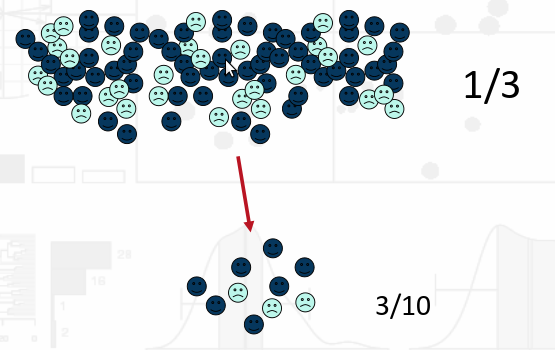
\includegraphics[scale=0.35]{ilu/bo.png}\end{center}\end{figure}
Imaginons que nous ayons une population de d�tenus. On sait que $\frac{1}{3}$ de ces derniers ont une symptomatologie d�pressive.\newline
On en tire au sort $10$ et on constate, en les interrogeant qu'il y en a $3$ parmis ces $10$ qui ont effectivement une symptomatologie d�pressive.\newline
\begin{figure}[H]\begin{center}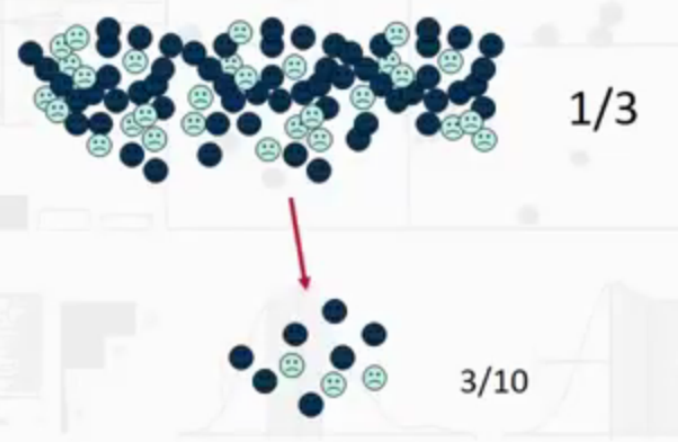
\includegraphics[scale=0.35]{ilu/bp.png}\end{center}\end{figure}
Dans la r�alit�, il est impossible de savoir si dans la population choisie pr�c�demment, il y a r�ellement $\frac{1}{3}$ des d�tenus qui ont une symptomatologie depressive. La question que l'on peut se poser est d�s lors que l'on r�int�gre l'�chantillon de d�tenus et que l'on consid�re l'ensemble de la population, \textit{combien d'entre eux sont r�ellement d�pressif}.\newline
On aurait tendance � r�pondre $30\%$; mais cela n'est vrai que si l'ensemble de la population est similaire � l'�chantillon que l'on a extrait (que l'�chantillon est dit repr�sentatif) ce qui n'est pas forc�ment le cas.\newline
En effet, il existe, dans ce cas ci, une infinit� de configurations possibles.
\begin{figure}[H]\begin{center}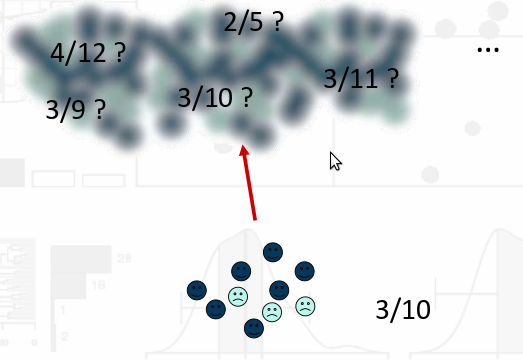
\includegraphics[scale=0.35]{ilu/bq.png}\end{center}\end{figure}
C'est � partir de ce moment que le calcul des probabilit� va intervenir.\newline
\\
En effet, on peut montrer que si l'on part d'une population globale - Dans notre cas, la population des d�tenus masculins des prisons de France M�tropolitaine - si l'on tire au sort un �chantillon de $10$ sujets dont $3$ ont une symptomatologie depressive, alors on peut montrer qu'il y a \textbf{95 chances sur 100 que dans la population totale des d�tenus, la v�ritable proportion des d�tenus pr�sentant cette caract�ristiques sera comprise entre 8\% et 64\%}.\newline
On dit ainsi que l'intervalle $[8\%,64\%]$ est un intervalle de confiance � $95\%$ de la pr�valence de la symptomatologie depressive.\newline
A ce stade, on peut consid�rer que l'intervalle est insuffisamment pr�cis. Cela s'explique par la taille de l'�chantillon (10 dans notre cas).\newline
\\
Imaginons alors que l'on tire au sort $100$ d�tenus, si $30\%$ sont d�prim�es alors il y a 95 chances sur 100 que la proportion de d�prim�s dans la population soit  comprise entre $21\%$ et $39\%$\newline
On dit ainsi que l'intervalle $[21\%,39\%]$ est un intervalle de confiance � $95\%$ de la pr�valence de la symptomatologie depressive.\newline
\\
A nouveau, Imaginons alors que l'on tire au sort $1000$ d�tenus, si $30\%$ sont d�prim�es alors il y a 95 chances sur 100 que la proportion de d�prim�s dans la population soit  comprise entre $27\%$ et $33\%$\newline
On dit ainsi que l'intervalle $[27\%,33\%]$ est un intervalle de confiance � $95\%$ de la pr�valence de la symptomatologie depressive.\newline
\\
\textbf{Note : } Plus la taille d'un �chantillon est grande, plus l'intervalle de confiance sera pr�cis.\newline
\\
\section{M�thode de calcul d'un intervalle de confiance}
En pratique, il s'agit d'un des derniers calculs que l'on va r�aliser � la main lors d'une �tude statistique.\newline
En effet, il existe une formule assez simple pour le d�terminer.\newline
Si nous sommes int�ress�s par un param�tre et que ce dernier \underline{suit une distribution Normale}, que l'on dispose d'un �chantillon tir� au sort dans une population et que l'on a estim� une valeur du param�tre, not� \textbf{m}, avec son �cart-type, not� $\sigma$, alors \textbf{l'intervalle de confiance � 95\% du param�tre} est donn� par : 
$$[m-1.96\times \sigma , m+1.96\times\sigma]$$
\textbf{Note : } Beaucoup de param�tres suivent une loi Normal, c'est notamment le cas de la moyenne et du pourcentage.\newline
\\
Un probl�me plus insidieux\footnote{Qui constitue un pi�ge, qui cherche � tromper} est que l'�chantillon doit �tre tir� au sort pour �tre r�ellement repr�sentatif d'une distribution. Or dans beaucoup d'�tudes, ces derniers ne le sont pas (Quand on interroge des individus avec un questionnaire, On ne tire pas ces derniers au sort, on va les rencontrer dans la rue, dans une classe ou sur internet).\newline
Quand un �chantillon n'est pas tir� au sort, alors l'intervalle de confiance perd en signification. Stricto sensu, un IC (intervalle de confiance) est d�finit pour un �chantillon construit al�atoirement. Quand l'�chantillon n'est pas pris al�atoirement, certains diront l'on ne peut rien en conclure et d'autre pr�ciseront que l'IC donne quand m�me une \textbf{id�e} de la fluctuation ou de la valeur possible d'un param�tre dans une population plus grande (et non pas une valeur de confiance car l'�chantillon n'a pas �t� tir� au sort).\newline
\\
Dans \textbf{R}, � l'aide de la librairie \textit{prettyR} et de la fonction \textbf{describe()}, il est possible d'estimer la moyenne et l'�cart type de l'�ge des d�tenus.
\begin{lstlisting}[language=html]
> smp <-read.csv2("/comptes/E131729J/XX_Universit�_fun/univfunR/TP/smp1.csv")
> library(prettyR)
> describe(smp$age)
> ##Application de la formule ci dessus
> borninf <- 38.9 - 1.96*(13.28/sqrt(797))
> borninf
[1] 37.97801
> bornsup <- 38.9 + 1.96*(13.28/sqrt(797))
> bornsup
[1] 39.82199
\end{lstlisting}
$$inf = \bar{x} - 1.96\times\frac{\sigma}{\sqrt{N}}\textrm{ et }sup = \bar{x} + 1.96\times\frac{\sigma}{\sqrt{N}}$$
On peut donc affirmer que sous r�serve que la distribution suive une loi Normale, alors l'intervalle de confiance � 95\% de l'�ge est obtenu par les valeurs.
$$[38,40] (\textrm{ans})$$
Voyons � pr�sent comment estimmer un intervalle de confiance � 95\% pour un pourcentage.\newline Nous allons supposer avoir un �chantillon de $10$ personnes. Dans ce dernier, nous avions observ� 3 individus pr�sentant une symptomatologie d�pressive, tir�s au sort dans une vaste population.\newline
Nous avions dis alors que l'intervalle de confiance � 95\% �tait � $[8\%,64\%]$.\newline
Pour estimer ces deux valeurs avec R, nous pouvons utiliser la librairie \textit{binom} et la fonction \textit{binom.confint()} avec pour param�tres la taille de l'�chantillon pr�lev�, la population totale.
\begin{lstlisting}[language=html]
> library(binom)
> binom.confint(3,10,method="all")
          method x  n      mean      lower     upper
1  agresti-coull 3 10 0.3000000 0.10333842 0.6076747
2     asymptotic 3 10 0.3000000 0.01597423 0.5840258
3          bayes 3 10 0.3181818 0.07454423 0.5794516
4        cloglog 3 10 0.3000000 0.07113449 0.5778673
5          exact 3 10 0.3000000 0.06673951 0.6524529
6          logit 3 10 0.3000000 0.09976832 0.6236819
7         probit 3 10 0.3000000 0.08991347 0.6150429
8        profile 3 10 0.3000000 0.08470272 0.6065091
9            lrt 3 10 0.3000000 0.08458545 0.6065389
10     prop.test 3 10 0.3000000 0.08094782 0.6463293
11        wilson 3 10 0.3000000 0.10779127 0.6032219
\end{lstlisting}

Le probl�me de cette fonction est qu'il n'existe pas une mais plusieurs m�thodes permettant de calculer des intervalles de confiance.\newline
Le statisticiens ne sont pas toujours d'accords sur la m�thode � utiliser car en effet, certaines sont utiles pour des petits effectifs, d'autres plus puissantes, \dots \newline
On s'int�resse alors � la ligne suivante car on y retrouve les valeurs que nous avons calcul� pr�c�demment. 

\begin{lstlisting}[language=html]
> binom.confint(3,10,method="prop.test")
     method x  n mean      lower     upper
1 prop.test 3 10  0.3 0.08094782 0.6463293
\end{lstlisting}
En pratique, si l'on souhaite utiliser une m�thode qui pr�sente le moins le probl�mes possibles, il faut choisir la m�thode \textit{exact} dont les r�sultats obtenus sont tr�s proches de nos r�sultats calcul�s : 
\begin{lstlisting}[language=html]
> binom.confint(3,10,method="exact")
  method x  n mean      lower     upper
1  exact 3 10  0.3 0.06673951 0.6524529
\end{lstlisting}
On peut consid�rer qu'il est un peu g�nant qu'il existe plusieurs m�thodes permettant de calculer un intervalle de confiance et que toute ne parviennent pas aux m�mes r�sultats. \newline
Heureusement, quand la taille de l'�chantillon est suffisamment grande, l'ensemble des m�thodes convergent vers une m�me valeur. Reprenons notre exemple pr�c�dent, non plus sur 10 sujets mais sur 1000 et 300 sympt�matologies observ�es : 
\begin{lstlisting}[language=html]
> binom.confint(300,1000,method="all")
          method   x    n      mean     lower     upper
1  agresti-coull 300 1000 0.3000000 0.2723966 0.3291341
2     asymptotic 300 1000 0.3000000 0.2715974 0.3284026
3          bayes 300 1000 0.3001998 0.2719448 0.3286787
4        cloglog 300 1000 0.3000000 0.2718595 0.3285966
5          exact 300 1000 0.3000000 0.2717211 0.3294617
6          logit 300 1000 0.3000000 0.2723865 0.3291466
7         probit 300 1000 0.3000000 0.2722277 0.3289871
8        profile 300 1000 0.3000000 0.2721340 0.3288893
9            lrt 300 1000 0.3000000 0.2721419 0.3289000
10     prop.test 300 1000 0.3000000 0.2719222 0.3296354
11        wilson 300 1000 0.3000000 0.2724068 0.3291239
\end{lstlisting}

Nous constatons alors que valeurs convergent toutes vers un l'intervalle de confiance : $$ [27\%,33\%]$$
%%%%%%%%%%%%%%%%%%%%%%%%%%%%%%%%%%%%%%%%%%%%%%%%%%%%%%%%%%%%%%%
%%%%%%%%%%%%%%%%%%%%%%%%%%%%%%%%%%%%%%%%%%%%%%%%%%%%%%%%%%%%%%%
%%%%%%%%%%%%%%%%%%%%%%%%%%%%%%%%%%%%%%%%%%%%%%%%%%%%%%%%%%%%%%%
\chapter{Mesure de la force de liaison entre deux variables quantitatives : Le coefficient de corr�lation}
Mesurer, quantifier, caract�riser la force de l'association existante entre deux mesures est � la base de la plupart des exp�riences scientifiques. Ainsi, le physicien va t'il chercher � caract�riser la relation qu'il observe entre la distance de chute d'un corps et sa vitesse. Le m�decin, quant � lui, sera plus int�ress� par la relation entre la tension art�rielle et la probabilit� d'apparition d'un infarctus.\newline
\\
\textit{Deux variables sont dites d�pendantes quand la connaissance de l'un donne une indication sur la valeur de l'autre}. Le niveau d'indication peut �tre plus o� moins �lev� et cela correspond � des liaisons plus ou moins fortes.\newline
Il est possible de parler de \textbf{Force} d'une liaison. Prenons en exemple un couple de jumeaux : 
\begin{itemize}
\item Si vous connaissez la taille d'un des deux jumeaux, alors cela nous donne une indication assez pr�cise sur la taille  du second jumeau. On dit alors que la relation est \textbf{forte}.
\item Si vous connaissez le revenu d'un des deux jumeaux, alors cela peux vous donner une indication statistique sur les revenus du second jumeau. Dans ce cas, la relation est \textbf{moins forte}.
\item Dans le cas o� les deux jumeaux vont tous les deux jouer au casino, le niveau des pertes et des gains du premier jumeau sera une tr�s maigre indication sur celles et ceux du second jumeau. On dira alors que la force de liaison est \textbf{tr�s faible voire nulle}.
\end{itemize}
Un quiproquo tr�s fr�quent en statistique est celui qui est entre \textbf{la liaison et la causalit�}. Ce n'est pas parce qu'il y a une liaison statistique que cela implique forc�ment une causalit� entre deux variables (l'inverse est �galement faux).\newline
Il existe une liaison entre le fait d'avoir les dents jaunes et le fait d'attraper un cancer du poumons car les fumeurs ont souvent les dents jaunes et que fumer est un facteur de risque du cancer du poumon. Mais bien entendu, il n'y a aucune relation de cause � effet (causalit�) entre avoir les dents jaunes et avoir un cancer du poumon.\newline
\\
Le grand classique pour quantifier la force de relation entre \textit{deux variables quantitatives} est le \textbf{coefficient de corr�lation de PEARSON} (Mais il y a mieux). Il faut avoir � l'esprit que la corr�lation de PEARSON est un cas particulier de liaison, liaison que l'on qualifie souvent de monotone ou de lin�aire :
\begin{center}
\textit{Soit X et Y, deux variables. Plus l'une est grande, plus l'autre le sera �galement.}
\end{center}  
Le coefficient de corr�lation est souvent d�signer par la lettre \textbf{r} et ce dernier \textit{varie entre $\pm 1$}. Quand $r=0$, de fa�on un peu h�tive, on consid�re que les deux variables sous jacentes sont ind�pendantes; Malheureusement ce n'est pas l'interpr�tation qu'il faut lui donner. \newline 
Il est vrai que dans le cas o� les deux variables suivent une loi Normale, il peut arriver que si l'une des deux variables ne suit pas r�ellement une loi Normale que $r$ soit �gal � 0 et pourtant, il y a bien une relation entre les deux variables (cas rare). \newline
Quand $r=\pm 1$, la force de la liaison est tellement importante que la connaissance d'une variable donne exactement la valeur de l'autre variable. On dit alors que les deux variables sont \textbf{mutuellement d�termin�e} au moyen d'une relation lin�aire du type :
$$Y=a\times X + b$$
Quand $r>0$, plus l'une des variables est grande, plus l'autre le sera �galement alors que quand $r<0$, quand une variable augmente, l'autre diminue. Par exemple, entre 0 et 6 ans, il y a une corr�lation positive assez forte entre la taille et l'�ge; En effet, plus l'enfant vieilli, plus il sera grand. Au contraire, � partir de 60 ans, il y a une corr�lation l�g�re mais n�gative entre l'�ge et la taille � cause de l'ost�oporose, plus on vieilli, plus on se tasse.\newline
\\
L'expression math�matique qui permet de traduire une corr�lation n'est pas si compliqu�e que �a : 
$$r=\frac{(x_{1}\cdot y_{1} + \dots + x_{n}\cdot y_{n})-n\times\bar{x}\times\bar{y}}{(n-1)\times \sigma(x)\times \sigma(y)}$$
Cette formule correspond � la covariance divis�e par la racine carr� des variances.\newline 
Nous avons vu pr�c�demment que la variance n'�tait pas facile � interpr�ter et naturellement, il se pose la question de l'interpr�tation de la taille et de l'importance de la valeur d'un coefficient de corr�lation.
\begin{center}
\begin{tabular}{|c|c|c|}\hline

\textbf{Corr�lation} &  	\textbf{N�gative} &  	\textbf{Positive} \\\hline
\textbf{Faible} 	& de -0,5 � 0,0 	& de 0,0 � 0,5 \\\hline
\textbf{Forte} &	de -1,0 � -0,5 &	de 0,5 � 1,0\\
\hline
\end{tabular}
\end{center}
Dans certains livres, il est dit que le pourcentage de variance partag� entre deux variables est �gal au carr� du coefficient de corr�lation. Cette assertion est math�matiquement vraie mais quel en est vraiment le sens. Soient x et y, deux variables qui corr�lent � 0,6, le pourcentage de variance partag� est donc de 0,36 soit 36\%. Cela ne signifie pas que les variables se ressemble seulement � 36 \%.\newline
Un fa�on d'interpr�ter ce qu'est une corr�lation de $0,6$ ou de $0,4$ est de r�aliser des simulation et d'analyser des graphiques en $(O,x,y)$.

\begin{figure}[H]\begin{center}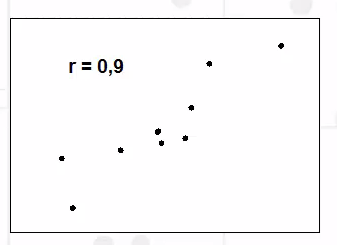
\includegraphics[scale=0.4]{ilu/br.png}\caption{Repr�sentation graphique d'une corr�lation � r=0,9 entre deux variables pour 10 individus}\end{center}\end{figure}
\begin{figure}[H]\begin{center}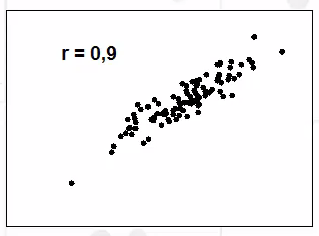
\includegraphics[scale=0.4]{ilu/bu.png}\caption{Repr�sentation graphique d'une corr�lation � r=0,9 entre deux variables pour 100 individus}\end{center}\end{figure}
\begin{figure}[H]\begin{center}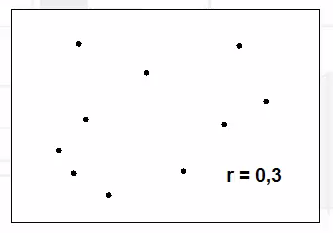
\includegraphics[scale=0.4]{ilu/bs.png}\caption{Repr�sentation graphique d'une corr�lation � r=0,3 entre deux variables pour 10 individus}\end{center}\end{figure}
\begin{figure}[H]\begin{center}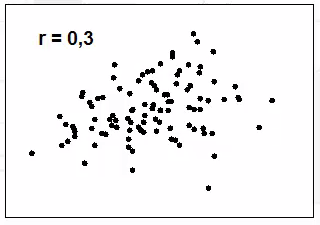
\includegraphics[scale=0.4]{ilu/bv.png}\caption{Repr�sentation graphique d'une corr�lation � r=0,3 entre deux variables pour 100 individus}\end{center}\end{figure}
\begin{figure}[H]\begin{center}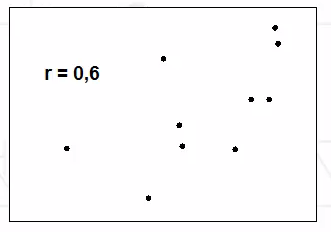
\includegraphics[scale=0.4]{ilu/bt.png}\caption{Repr�sentation graphique d'une corr�lation � r=0,6 entre deux variables pour 10 individus}\end{center}\end{figure}
\begin{figure}[H]\begin{center}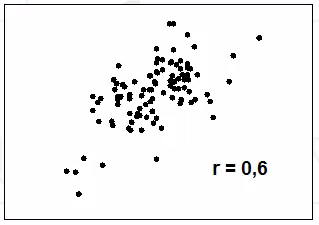
\includegraphics[scale=0.4]{ilu/bw.png}\caption{Repr�sentation graphique d'une corr�lation � r=0,6 entre deux variables pour 100 individus}\end{center}\end{figure}
On voit que pour $r=0.9$, l'association entre $x$ et $y$ est �vidente alors que pour $r=0.3$ et � l'oeil nu, il est difficile d'affirmer que d�s lors que 
$x$ est grand, $y$ l'est aussi.\newline
\\
Nous allons voir comment calculer avec \textbf{R}, un coefficient de coefficient de PEARSON. Dans l'�tude sur la sant� mentale en prison, nous allons calculer le coefficient de corr�lation entre l'�ge et le nombre d'enfant.
\begin{lstlisting}[language=html]
> setwd("~/Desktop/DIVERS + TEMPLATES/R/TP")
> smp.c <- read.csv2("/Users/mehdilatif/Desktop/DIVERS + TEMPLATES/R/TP/smp2.csv")
> table(smp.c$age)
19 20 21 22 23 24 25 26 27 28 29 30 31 32 33 34 35 36 37 38 39 40 41 42 43 44 
45 46 47 48 49 50 51 52 53 54 55 15 15 18 13 23 30 22 30 25 21 20 25 18 22 26 
20 16 18 25 24 23 22 23 19 17 19 17 16 12 17 23 16 11 10  8 11  6 56 57 58 59 
60 61 62 63 64 65 66 67 68 69 70 71 72 73 74 77 79 81 83 14  9  7  6  7  5  7  
4  5  3  6  4  2  1  1  6  3  2  2  3  1  1  2 

> table(smp.c$n.enfant)
  0   1   2   3   4   5   6   7   8   9  10  11  13 
214 220 125 101  55  31   7   7   7   2   2   1   1 
> plot(jitter(smp.c$age),jitter(smp.c$n.enfant))
\end{lstlisting}

\begin{figure}[H]\begin{center}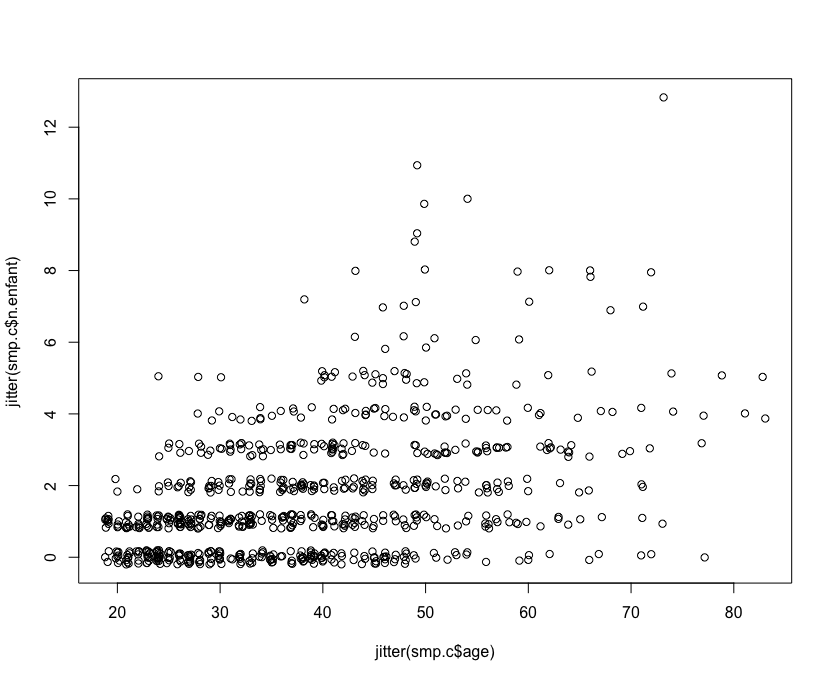
\includegraphics[scale=0.5]{ilu/bx.png}\end{center}\end{figure}

La fonction qui permet de calculer un coefficient de corr�lation de PEARSON sous \textbf{R} est la suivante :\newline
\textbf{Attention : } Ne pas oublier le param�tre \textit{use="complete.obs"} qui permet de g�rer les donn�es manquantes.
\begin{lstlisting}[language=html]
> cor(smp.c$age,smp.c$n.enfant,use="complete.obs")
[1] 0.4326039
\end{lstlisting}
Il est important de garder � l'esprit que le coefficient de corr�lation ne r�pond pas � toute les questions concernant la quantification des relations entre deux variables quantitatives. Non seulement deux variables peuvent �tre li�es alors que leurs corr�lation est nulle (cas des relation quadratique entre deux variables).\newline
Il existe �galement des situations o� la forme de la liaison entre $x$ et $y$ qui int�resse les exp�rimentateurs ne correspond pas � la corr�lation de PEARSON. C'est notamment le cas lorsque l'on s'int�resse � la \textbf{concordance} entre deux variables al�atoires\footnote{L'accord observ� entre des jugements qualitatifs ou non, r�sulte de la somme d'une composante �al�atoire� et d'une composante d'accord �v�ritable�.Le coefficient Kappa $K$ propose de chiffrer l'intensit� ou la qualit� de l'accord r�el entre des jugements qualitatifs appari�s.Il exprime une diff�rence relative entre la proportion d'accord observ�e $P_{0}$ et la proportion d'accord al�atoire $P_{e}$ qui est la valeur esp�r�e sous l'hypoth�se nulle d'ind�pendance des jugements, divis�e par la quantit� disponible au-del� de l'accord al�atoire. En d�finitive, K est un pourcentage de l'accord maximum corrig� de ce qu'il serait sous le simple effet du hasard. La valeur vraie du coefficient Kappa dans la population est une variable al�atoire qui suit approximativement une loi de Gauss de moyenne $K$ et de variance $Var(K)$. L'hypoth�se nulle $H_{0}$ est K = 0 contre l'hypoth�se alternative $H_{1}$ : $K > 0$. Dans le cas d'une �tude d'accord entre deux observateurs statistiquement ind�pendants ayant r modalit�s de jugement, avec $r^{3}2$, le coefficient Kappa s'�crit : $\frac{P_{0}-P_{e}}{1-P_{e}}$ avec $P_{0}$ : la proportion d'accord observ�e et $P_{e}$ : la proportion d'accord al�atoire ou concordance attendue sous l'hypoth�se d'ind�pendance des jugement.}. 
Ou alors, deux biologistes qui tentent de calibrer un appareil, un nouvel appareil qui ne co�te pas tr�s cher au moyen d'un autre appareil qui lui est une r�f�rence parce qu'il co�te tr�s cher. Dans ce type de situation, si le nouvel appareil dit syst�matiquement un r�sultat deux fois moins important que l'appareil de r�f�rence, alors la corr�lation sera parfaite, elle vaudra $1$ et pourtant le nouvel appareil sera bien mauvais puisque syst�matiquement il donne un r�sultat faux.
%%%%%%%%%%%%%%%%%%%%%%%%%%%%%%%%%%%%%%%%%%%%%%%%%%%%%%%%%%%%%%%
%%%%%%%%%%%%%%%%%%%%%%%%%%%%%%%%%%%%%%%%%%%%%%%%%%%%%%%%%%%%%%%
%%%%%%%%%%%%%%%%%%%%%%%%%%%%%%%%%%%%%%%%%%%%%%%%%%%%%%%%%%%%%%%
\chapter{Risque relatif et odds-ratio}
Dans ne nombreuses disciplines, nous sommes amen�s � nous int�resser � la  quantification de la force de liaison entre deux variables binaires. le genre et le fait d'�tre oui ou non au ch�mage. En m�decine, un cas tr�s fr�quent est celui de l'association entre une maladie et un facteur de risque, par exemple celui d'�tre fumeur et de d�velopper plus tard un infarctus du myocarde ou plus g�n�ralement une pathologie coronarienne.\newline
Pour entrer deans le d�tail, nous allons consid�rer le cas particulier de la relation entre une maladie et un facteur de risque. Les donn�es peuvent �tre repr�sent�es au moyen d'un tableau comme celui ci dessous : 

\begin{center}
\begin{tabular}{l|l|l|ll}
\cline{2-3}
 & \multicolumn{2}{l|}{\textbf{Maladie}} &  &  \\ \cline{2-3}
 & \textit{Oui} & \textit{Non} &  &  \\ \cline{1-3}
\multicolumn{1}{|l|}{\textbf{FR = "Oui"}} & a & b &  &  \\ \cline{1-3}
\multicolumn{1}{|l|}{\textbf{FR = "Non"}} & c & d &  &  \\  \cline{1-3}
\end{tabular}
\end{center}
On y repr�sente en colonne les individus malades (\textit{oui}) et non malades (\textit{non}) et en ligne, les sujets ayant un facteur de risque (\textit{FR="Oui"}) et ceux qui n'en ont pas (\textit{FR="Non"}).\newline
Le param�tre le plus intuitif pour quantifier la force de l'association entre cette maladie et ce facteur de risque  est le \textbf{Risque Relatif (RR)} qui repr�sente le pourcentage de sujets malades parmi ceux qui ont un facteur de risque divis� par le pourcentage de sujets malades chez ceux qui ne sont pas porteurs du facteur de risque : 
$$\mathbf{\textrm{RR}} = \frac{\frac{a}{a+b}}{\frac{c}{c+d}}$$
Nous avons l� un param�tre simple et facile � interpr�ter.\newline
\\
Le risque relatif n'est pas le seul param�tre que l'on peut utiliser dans cette situation. Il existe aussi l'\textbf{Odds-ratio}. Ce dernier est parfois traduit par \textit{Rapport des cotes} (au sens valeur \dots cot� en bourse).\newline
Il se calcul comme le rapport entre le rapport des individus malades sur ceux qui ne le sont pas, sachant que les deux ont un facteur de risque, sur le rapport des individus malade sur ceux qui ne le sont pas sachant qu'ils n'ont pas de facteur de risque : 
$$\mathbf{\textrm{OR}} = \frac{\frac{a}{b}}{\frac{c}{d}}$$
A l'�vidence, l'Odds-ratio est moins intuitif que le Risque Relatif.
\section{Odds-ratio VS Risque Relatif}
L'Odds-ratio a un inconv�nient �vident, on ne sait pas trop ce qu'il mesure au contraire du risque relatif qui lui a un sens clair et pr�cis que tout le monde appr�hende facilement.\newline
\\
Cependant, L'Odds-ratio pr�sente de nombreux avantages.\newline
En effet, il permet la gestion des facteurs de confusion. Imaginons que nous souhaitions mettre en �vidence un association entre ob�sit� et infarctus du myocarde. Il suffit de montrer qu'il y a une relation (association) statistiquement significative mais nous avons du mal � l'interpr�ter car il est possible que ce ne soit pas l'ob�sit� en elle m�me qui soit associ�e � l'infarctus du myocarde mais peut �tre que cette derni�re est associ�e � une faible pratique du sport et que c'est l'absence de pratique du sport qui g�n�re ce risque d'infarctus du myocarde.\newline
Pour r�pondre � cette question de sant� publique, une solution possible est d'utiliser un mod�le statistique qui va permettre de trouver le poids sp�cifique de l'ob�sit� et de la pratique du sport sur la survenue de l'infarctus du myocarde(R�gression logistique, tr�s utile pour d�terminer des relations complexes entre es variables "binaires"). Ces mod�les permettent assez facilement d'estimer des Odds-ratios ajust�s et beaucoup plus difficilement des Risques Relatifs ajust�s. 
D'o� la recherche de l'Odds-ratio qui peut �tre g�n�raliser au cas de la recherche de facteurs de confusion.\newline
\\
De plus, l'Odds-ratio peut �tre utilis� dans les enqu�tes dites \textit{cas-t�moin}\footnote{�tude statistique observationnelle r�trospective utilis�e en �pid�miologie. Les �tudes cas-t�moins sont utilis�es pour mettre en �vidence des facteurs qui peuvent contribuer � l'apparition d'une maladie en comparant des sujets qui ont cette maladie (les cas) avec des sujets qui n'ont pas la maladie mais qui sont similaires par ailleurs (les t�moins).} Pour �valuer un Odds-ratio ou un Risque Relatif, par exemple pour d�terminer la relation entre l'ob�sit� et le risque d'infarctus du myocarde, on peut r�aliser une enqu�te en population g�n�rale c'est � dire tirer au sort un nombre suffisamment grand de personnes (1000 voir 10000) dans la population g�n�rale et leurs demander si ils ont d�j� eu un infarctus du myocarde et �galement regarder si ils sont ob�se ou non.\newline
On r�aliser alors le tableau suivant : 
\begin{center}
\begin{tabular}{l|l|l|ll}
\cline{2-3}
 & \multicolumn{2}{l|}{\textbf{Infarctus du myocarde}} &  &  \\ \cline{2-3}
 & \textit{Oui} & \textit{Non} &  &  \\ \cline{1-3}
\multicolumn{1}{|l|}{\textbf{Ob�se = "Oui"}} & a & b &  &  \\ \cline{1-3}
\multicolumn{1}{|l|}{\textbf{Ob�se = "Non"}} & c & d &  &  \\  \cline{1-3} 
\end{tabular}
\end{center}
On peut donc calculer les Risques Relatif et le Odds-ratio correspondants � cette �tude.\newline
Mais pour pouvoir calculer ces param�tres avec suffisamment de pr�cision et compte tenu de la raret� de l'infarctus du myocarde, il va falloir inclure dans l'�tude un grand nombre de sujet et il est possible que 1000 ou 10000 sujets ne soient pas suffisants.\newline
Ce type d'�tude va donc vite devenir tr�s on�reux. \newline
Un fa�on de r�aliser ce type d'�tude � bas co�t est de r�aliser cette �tude sur $X$ sujets sains et $X$ sujets atteints d'un infarctus du myocarde. C'est ce que l'on appelle une �tude de cas-t�moins. Dans le cadre de ces �tudes, une centaine de cas et de t�moins peuvent suffire.\newline
La question est maintenant de savoir si le calcul d'un Risque Relatif ou d'un Odds-ratio est possible � partir ce type d'enqu�te.\newline
Il s'av�re que la r�ponse est \textbf{Non avec un Risque Relatif } et \textbf{Oui avec un Odds-ratio}.\newline
\\
Enfin, l'argument conclusif est que certes, l'Odds-ratio est difficilement interpr�table mais quand le facteur �tudi� (dans notre cas, l'infarctus du myocarde) est suffisamment rare, c'est � dire que sa pr�valence est inf�rieure � 5\%, alors l'Odds-ratio tend � �tre �quivalent au Risque Relatif.\newline
\\ 
Nous pouvons nous interroger l�gitiment sur le fait que \textit{l'Odds-ratio puisse �tre estim� � la fois dans une enqu�te cas-t�moins et dans une enqu�te en population g�n�rale}\footnote{Population g�n�rale : t�moins tir�s au sort sur listes �lectorales, liste t�l�phonique (random digit dialing)\dots Epid�miologie de population (population g�n�rale) - Descriptif : R�partition et fr�quence d'une maladie - Analytique : Recherche de facteurs de risque - Evaluatif : Evaluation d'action de sant� publique (action de pr�vention, de d�pistage \dots)} alors que \textit{le Risque Relatif ne peut �tre calcul� que dans le cadre d'une enqu�te en population g�n�rale}.\newline
\\
Pour en �tre convaincu, analysons l'exemple suivant o� nous allons chercher une relation entre le fait de fumer et d'�tre enrhum�  :

\begin{center}
\begin{tabular}{l|l|l|ll}
\cline{2-3}
 & \multicolumn{2}{l|}{\textbf{Rhume}} &  &  \\ \cline{2-3}
 & \textit{Oui} & \textit{Non} &  &  \\ \cline{1-3}
\multicolumn{1}{|l|}{\textbf{Tabac = "Oui"}} & 30 & 300 &  &  \\ \cline{1-3}
\multicolumn{1}{|l|}{\textbf{Tabac = "Non"}} & 30 & 600 &  &  \\  \cline{1-3}
\end{tabular}
\end{center}
Dans cette �tude, nous avons simul� une enqu�te aupr�s de 1000 sujets.
$$\mathbf{\textrm{RR}} = \frac{\frac{30}{300+30}}{\frac{30}{600+30}} = 1,91$$
$$\mathbf{\textrm{OR}} = \frac{\frac{30}{300}}{\frac{30}{600}}=2$$.

On constate, comme c'est g�n�ralement le cas, que l'\textbf{Odds-ration surestime le Risque relatif}.\newline  
\\
Imaginons maintenant que l'on r�alise une enqu�te cas-t�moins o� nous allons �tudier 90 personnes non enrhum�es, 60 personnes enrhum�es avec, pour chacun, un niveau d'exposition au tabac exactement similaire � celui de l'�tude que l'on a r�alis� pr�c�demment :
\begin{center}
\begin{tabular}{l|l|l|ll}
\cline{2-3}
 & \multicolumn{2}{l|}{\textbf{Rhume}} &  &  \\ \cline{2-3}
 & \textit{Oui} & \textit{Non} &  &  \\ \cline{1-3}
\multicolumn{1}{|l|}{\textbf{Tabac = "Oui"}} & 30 & 30 &  &  \\ \cline{1-3}
\multicolumn{1}{|l|}{\textbf{Tabac = "Non"}} & 30 & 60 &  &  \\ \cline{1-3}
\end{tabular}
\end{center}

$$\mathbf{\textrm{RR}} = \frac{\frac{30}{30+30}}{\frac{30}{60+30}} = 1,5$$
$$\mathbf{\textrm{OR}} = \frac{\frac{30}{30}}{\frac{30}{60}}=2$$.
Nous avons d�s lors, un Risque Relatif de 1.5, inf�rieur � celui de la premi�re �tude alors que l'Odds-ratio est toujours �gal � 2.\newline
On peut donc en d�duire que l'Odds-ration est plus stable que le Risque Relatif.\newline
\\
Passons maintenant � un cas concret : Nous allons essayer de d�terminer dans quelle mesure un niveau �lev� d'�vitement du danger est associ� � un trouble d�pressif.\newline
D�s lors, nous rencontrons un premier probl�me. En effet, la variable �vitement du danger (\textit{ed}) est cod�e en trois classe : 
\begin{enumerate}
\item Faible 
\item Mod�r�e 
\item Elev�e
\end{enumerate}
Il faut donc la red�finir en variable binaire que nous allons appeler \textit{ed.bin} ou les valeurs 1 (Faible) et 2 (Mod�r�e) seront cod�es en 0 et 3 (Elev�e) sera cod�e en 1.
\begin{lstlisting}[language=html]
> smp <-read.csv2("/comptes/E131729J/XX_Universit�_fun/univfunR/TP/smp1.csv")
> setwd("~/XX_Universit�_fun/univfunR/TP")

> ##variable de mesure d'�vitement du danger avant encodage binaire

> table(smp$ed,useNA = "always")
   1    2    3 <NA> 
 315  155  222  107 

> ##variable de mesure d'�vitement du danger apr�s encodage binaire

> ### SI la valeur de ed est sup�rieure stricte � 2 (=3 -> forte), alors smp$ed.bin[i] = 1, sinon smp$ed.bin[i]=0

> smp$ed.bin <- ifelse(smp$ed>2,1,0)

> table(smp$ed.bin,useNA = "always")

   0    1 <NA> 
 470  222  107 

> ##Analyse � l'oeil nu des valeurs avant et ap�s modification

> str(smp)
'data.frame':	799 obs. of  10 variables:
 $ age      : int  31 49 50 47 23 34 24 52 42 45 ...
 $ prof     : Factor w/ 8 levels "agriculteur",..: 3 NA 7 6 8 6 3 2 6 6 ...
 $ dep.cons : int  0 0 0 0 1 0 1 0 1 0 ...
 $ scz.cons : int  0 0 0 0 0 0 0 0 0 0 ...
 $ grav.cons: int  1 2 2 1 2 1 5 1 5 5 ...
 $ n.enfant : int  2 7 2 0 1 3 5 2 1 2 ...
 $ rs       : int  2 2 2 2 2 1 3 2 3 2 ...
 $ ed       : int  1 2 3 2 2 2 3 2 3 2 ...
 $ dr       : int  1 1 2 2 2 1 2 2 1 2 ...
 $ ed.bin   : num  0 0 1 0 0 0 1 0 1 0 ...

> ##Analyse crois�e de ed.bin par rapport � ed gr�ce � la fonction table :

> table(smp$ed.bin,smp$ed,useNA = "always")      
         1   2   3 <NA>
  0    315 155   0    0
  1      0   0 222    0
  <NA>   0   0   0  107
  
> ###Ajout du nom des variables

> table(smp$ed.bin,smp$ed,deparse.level = 2,useNA = "always")
          smp$ed
smp$ed.bin   1   2   3 <NA>
      0    315 155   0    0
      1      0   0 222    0
      <NA>   0   0   0  107
\end{lstlisting}

Pour \textit{ed = 1} et \textit{ed = 2} nous obtenons \textit{ed.bin = 0} et pour \textit{ed = 3}, nous avons bien \textit{ed.bin = 1}.\newline

\begin{figure}[H]\begin{center}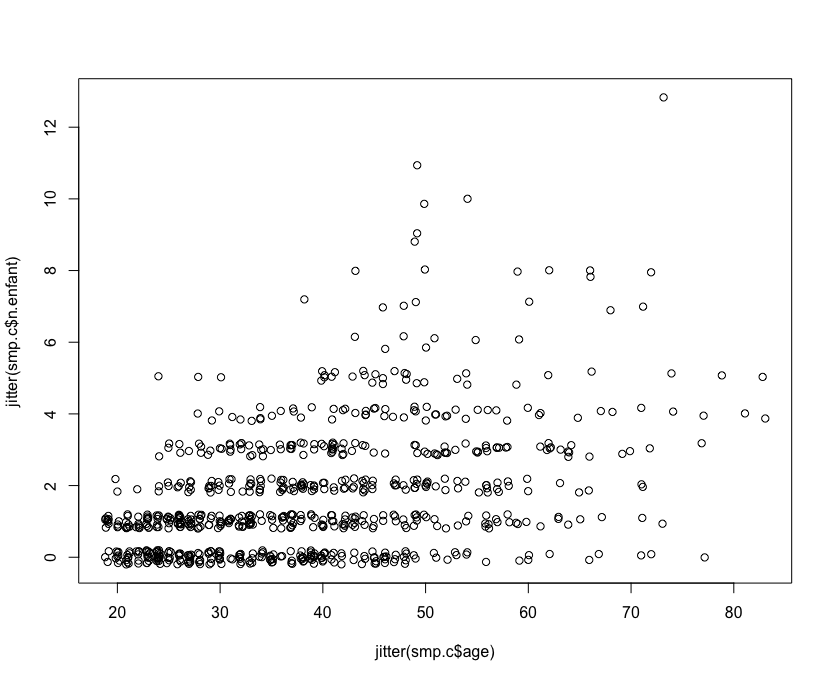
\includegraphics[scale=0.5]{ilu/bx.png}\end{center}\end{figure}
Calculons maintenant l'Odds-Ration et le Risque relatif pour �tablir une relation entre l'�vitement du danger et la symptomatologie d�pressive. Nous allons devoir faire appel � la libraire \textit{Epi} et utiliser la fonction \textit{twoby2()}.\newline
\textbf{Attention : } Il nous faut modifier les param�tres de la fonction \textit{twoby2()} et lui passer \textit{1-ed.bin} et {1-dep.cons}. Cette variation vient du fait que par d�faut, la fonction \textit{twoby2()} consid�re que lorsqu'une variable est cod�e en binaire :
\begin{itemize}
\item 0 signifie que l'on est malade et 1 signifie que l'on est pas malade
\item 0 signifie que l'on a le facteur de risque et 1, que l'on ne poss�de pas le facteur de risque. 
\end{itemize} 
Alors que dans notre jeu de donn�es, c'est exactement l'inverse.
\begin{lstlisting}[language=html]
> twoby2(1-smp$ed.bin,1-smp$dep.cons)
2 by 2 table analysis: 
------------------------------------------------------ 
Outcome   : 0 
Comparing : 0 vs. 1 

    0   1    P(0) 95% conf. interval
0 126  96  0.5676    0.5016   0.6312
1 135 335  0.2872    0.2481   0.3298

                                   95% conf. interval
             Relative Risk: 1.9760    1.6456   2.3726
         Sample Odds Ratio: 3.2569    2.3361   4.5408
Conditional MLE Odds Ratio: 3.2508    2.3037   4.6035
    Probability difference: 0.2803    0.2020   0.3549

             Exact P-value: 0 
        Asymptotic P-value: 0 
------------------------------------------------------
\end{lstlisting}
On obtient donc un Risque Relatif � 1.97 et un Odds-Ratio � 3.26. \newline
Dans ce cas, l'Odds-Ratio est "assez sensiblement" diff�rent du risque relatif car nous sommes dans une situation o� la pr�valence de la maladie n'est pas faible. En effet, dans notre �tude, entre 30 et 40\% des d�tenus pr�sentent un symptomatologie d�pressive. Nous ne sommes donc pas de la cas d'une pathologie rare (comme dans notre �tude de l'infarctus du myocarde) et donc l'Odds-Ratio est tr�s difficilement interpr�table.\newline
Il nous faudra alors nous focaliser sur le Risque Relatif  $\simeq$ 2.\newline 
\textbf{On peut donc en d�duire que l'on a deux fois plus de risque de pr�senter un �tat d�pressif lorsque l'on a un niveau d'�vitement du danger �lev� par rapport au contraire}.
%%%%%%%%%%%%%%%%%%%%%%%%%%%%%%%%%%%%%%%%%%%%%%%%%%%%%%%%%%%%%%%
%%%%%%%%%%%%%%%%%%%%%%%%%%%%%%%%%%%%%%%%%%%%%%%%%%%%%%%%%%%%%%%
%%%%%%%%%%%%%%%%%%%%%%%%%%%%%%%%%%%%%%%%%%%%%%%%%%%%%%%%%%%%%%%
\chapter{Tests statistiques : le "p" }
Dans les sciences de la vie, les sciences humaines et sociales, lorsque l'on fait une d�couverte, il faut d'abord s'assurer qu'elle n'est pas d� au hasard. \newline
C'est � cela que servent les \textbf{tests statistiques}.\newline
\\
Les tests statistiques sont souvent consid�r�s comme un domaine un peu basique de la science statistique mais en r�alit�, ce sont des techniques qui sont tr�s d�licates � comprendre.\newline
Nous allons commencer simplement par \textbf{le test du p} ou \textbf{p-value} que l'on retrouve dans de nombreuses publications scientifiques.\newline
\\
Dans le chapitre pr�c�dent, nous avons calcul� la corr�lation entre l'�ge des d�tenus et leurs nombres d'enfants : 
\begin{lstlisting}[language=html]
> smp <-read.csv2("/comptes/E131729J/XX_Universit�_fun/univfunR/TP/smp1.csv")
> setwd("~/XX_Universit�_fun/univfunR/TP")
> str(smp)
'data.frame':	799 obs. of  9 variables:
 $ age      : int  31 49 50 47 23 34 24 52 42 45 ...
 $ prof     : Factor w/ 8 levels "agriculteur",..: 3 NA 7 6 8 6 3 2 6 6 ...
 $ dep.cons : int  0 0 0 0 1 0 1 0 1 0 ...
 $ scz.cons : int  0 0 0 0 0 0 0 0 0 0 ...
 $ grav.cons: int  1 2 2 1 2 1 5 1 5 5 ...
 $ n.enfant : int  2 7 2 0 1 3 5 2 1 2 ...
 $ rs       : int  2 2 2 2 2 1 3 2 3 2 ...
 $ ed       : int  1 2 3 2 2 2 3 2 3 2 ...
 $ dr       : int  1 1 2 2 2 1 2 2 1 2 ...
> cor(smp$age,smp$n.enfant,use="complete.obs")
[1] 0.4326039
\end{lstlisting}
Cette corr�lation vaut $0.4$, elle est positive et substantielle\footnote{Qui est important}.\newline
\\
Cependant, on peut se demander dans quelle mesure le hasard pourrait expliquer � lui tout seul une telle corr�lation. En effet, si nous prenons n'importe quelle paire de variable, il se peut que par hasard, la corr�lation entre ces deux variables soit non nulle.\newline
Voyons cela sur un autre exemple : \textit{Prenons 2 d�s, un dans chaque mains et lanc�s ces derniers 10 fois}. On peut obtenir les r�sultats suivants (avec des r�sultats de mesures quantitatives comprises entre 1 et 6).
\begin{center}
\begin{tabular}{|c|c|c|c|c|c|c|c|c|c|c|}
\hline
\textbf{MG} & 3 & 3 & 6 & 5 & 1 & 4 & 1 & 6 & 5 & 5 \\ \hline
\textbf{MD} & 4 & 5 & 2 & 3 & 5 & 4 & 5 & 5 & 4 & 4 \\ \hline
\end{tabular}
\end{center}
Il est possible de calculer un coefficient de corr�lation entre les variables \textbf{MG} (Main Gauche) et \textbf{MD} (Main Droite). Ici, par construction, on sait qu'il n'existe pas de corr�lation entre ces deux r�sultats.\newline
N�anmoins, � partir des donn�es pr�sent�es ci dessus, on obtient une corr�lation \textbf{r=-0.6}.\newline
Cela signifie qu'en pratique, si l'on r�alise une experience mesurant deux variables quantitatives \underline{totalement ind�pendantes} sur 10 sujets, on peut tr�s bien obtenir par le simple effet du hasard, un coefficient de corr�lation non nul et aussi important que $|r|=0.6$\newline 
\\
Cette part de hasard dans les r�sultats de cette exp�rience peut avoir peut avoir des cons�quences tr�s g�nantes quand on fait de la recherche.\newline
En effet, si nous nous trouvons dans le cadre d'un essai th�rapeutique et que l'on compare les effets d'un m�dicament A � un m�dicament B. Apr�s tirage au sort et protocole en double aveugle\footnote{L'�tude randomis�e en double aveugle, avec r�partition al�atoire est une d�marche exp�rimentale utilis�e dans de nombreuses disciplines de recherche tels la m�decine, les sciences sociales et la psychologie,\dots. En pharmacie, elle est utilis�e dans le d�veloppement de nouveaux m�dicaments, et pour �valuer l'efficacit� d'une d�marche, d'un traitement.} r�alis� dans des circonstances optimales, nous obtenons la gu�rison de 40 \% dans le groupe ayant pris le m�dicament A et de 30\% dans celui qui a pris le m�dicament B, La question que l'on peut se poser est : Dans quelle mesure puis je dire que la diff�rence observ�e entre les deux traitements provient bien d'une diff�rence d'efficacit� et non d'un simple effet al�atoire provenant de la randomisation\footnote{M�thode de r�partition fond�e sur le hasard.La randomisation est une m�thode qui permet d'introduire un �l�ment al�atoire dans une �tude.} entre les deux groupes.\newline
\\
Revenons plus pr�cis�ment sur cet exemple : il s'agit d'un essai th�rapeutique randomis� (c'est � dire que l'on a tir� au sort l'attribution du m�dicament A ou du m�dicament B pour chaque patients). \newline
100 patients ont re�u le m�dicament A et 100 patients ont re�us le m�dicament B; 40 patients sur 100 (40\%) ont gu�ri avec A et 30 patients avec B (30\%). A l'�vidence, \textit{A est plus efficace que B}.\newline
N�anmoins, on peut se poser la question suivante : \textit{Est ce que le diff�rentiel d'efficacit� de 10\% est significatif ou est il compatible avec les in�vitables fluctuations issues du tirage au sort ?}\newline
\\
Pour r�pondre � cette question, nous allons tenter de la reformuler en la formalisant davantage : \newline
Imaginons que A et B soit d'une efficacit� �quivalente, Quelle est l'estimation la plus probable de l'efficacit� de A (ici, �gale � l'efficacit� de B) ?\newline 
Comme A et B ont la m�me efficacit�, on peut m�langer le groupe ayant re�u le traitement A avec celui ayant re�u le m�dicament B. En m�langeant ces deux groupes, le taux de gu�rison est la moyenne des taux de gu�rison individuel de chaque groupe c'est � dire 35\%.\newline
Nous avons donc un population de patients �ligibles qui peuvent recevoir les traitements A ou B et l'efficacit� de A est �gale � celle de B. On peut en d�duire que l'efficacit� du traitement que va recevoir chaque patient est de 35\%.\newline
Si partant de cette population, on s�lectionne 100 patients qui vont recevoir A et 100 patients qui vont recevoir B, quelle est l'estimation la plus probable du taux de gu�rison avec chaque m�dicaments ?\newline
Si tout se passe dans l'id�al, alors 35 patients vont gu�rir avec A et 35 patients avec B. Cependant, en pratique, il est tout a fait possible que cela ne se passe pas comme �a ; Il est possible que 36 personnes gu�rissent avec A et 37 avec B. Il est m�me possible que 40 personnes gu�rissent avec A et 30 avec B \dots La question que l'on doit se poser � ce stade de l'exp�rimentation est : \textit{Dans quelle mesure la diff�rence de 10\% que nous avons observ�e entre l'efficacit� dans le groupe A et l'efficacit� dans le groupe B est elle compatible avec un tirage au sort r�alis� dans une population o� 35\% des sujets vont gu�rir ?}\newline
\\
Nous avons l� exactement la d�finition de \textbf{p} � savoir, la probabilit� que le hasard puisse expliquer � lui seul une diff�rence d'efficacit� au moins aussi importante que celle que l'on a observ�. 
$$p = P\left((|\textrm{Gu�rison}_{A_{\%}} - \textrm{ Gu�rison}_{B_{\%}}|>10\%)\|\textrm{Gu�rison}_{Globale_{\%}} = 35\%\right)$$
Il est possible de calculer cette probabilit� et dans le cas qui nous int�resse, on trouve $p=0,14$.\newline
Il y a donc 14\% de chance que le hasard puisse expliquer � lui seul que 40\% des sujets ont gu�ris avec A et 30\% avec B ou d'une diff�rence encore plus importante d'efficacit�.\newline
En pratique, 14\% c'est trop. On va donc consid�rer que la diff�rence d'efficacit� entre les deux medicaments n'est pas significative. La r�gle tacite commun�ment admise est de consid�rer que si la probabilit� de p avait �t� inf�rieur � 5\%, alors il aurait �t� possible de dire que la diff�rence d'efficacit� est statistique significative. 
\subsection*{Introduction de la valeur-p par Ronald Fisher}
Le statisticien Ronald Fisher a introduit les termes de significativit�, d'hypoth�se nulle, et l'utilisation de la valeur-p. Il rejetait toutefois la notion de puissance statistique : selon lui, l'hypoth�se nulle ne peut jamais �tre accept�e, mais peut seulement �tre rejet�e par le test statistique. Dans cette approche, la valeur-p est consid�r�e comme une mesure d'� quel point les donn�es plaident contre l'hypoth�se nulle. Les seuils suivants sont g�n�ralement pris pour r�f�rence :
\begin{itemize}
\item   $p\leq 0.01$ : tr�s forte pr�somption contre l'hypoth�se nulle
\item $ 0.01<p\leq 0.05$ : forte pr�somption contre l'hypoth�se nulle
\item $0.05<p\leq 0.1$ : faible pr�somption contre l'hypoth�se nulle
\item $ p>0.1$ : pas de pr�somption contre l'hypoth�se nulle
\end{itemize}
Pour un diff�rentiel d'efficacit� constant, la valeur de \textbf{p} d�pend tr�s fortement de la taille des groupes compar�s. En effet, dans les m�me exemple : 
\begin{itemize}
\item Pour 100 sujets par groupe, $p=0.14$
\item Pour 200 sujets par groupe, $p=0.036$
\item Pour 1000 sujets par groupe, $p=0.000003$
\end{itemize}
Nous voyons ainsi qu'avec de grands �chantillons, l'influence possible du hasard diminue consid�rablement.
%%%%%%%%%%%%%%%%%%%%%%%%%%%%%%%%%%%%%%%%%%%%%%%%%%%%%%%%%%%%%%%
%%%%%%%%%%%%%%%%%%%%%%%%%%%%%%%%%%%%%%%%%%%%%%%%%%%%%%%%%%%%%%%
%%%%%%%%%%%%%%%%%%%%%%%%%%%%%%%%%%%%%%%%%%%%%%%%%%%%%%%%%%%%%%%
\chapter{L'approche de Neyman et Pearson :}
Nous avons vu dans le chapitre pr�c�dent le principe du test du p-value. Il faut d'ailleurs constater que dans la r�alit� des travaux scientifiques, les tests statistiques se r�sument � une succession de test du p-value.\newline
Cependant, dans le cadre scolaire, on apprend � utiliser les tests statistiques et non le p-value. L'un des principes des tests statistiques est celle de la th�orie des tests d'hypoth�ses de \textbf{NEYMAN \& PEARSON}.\newline
\\
Les test d'hypoth�ses selon la th�orie de NEYMAN \& PEARSON reposent sur une formulation assez formelle ; De mani�re assez simpliste, nous allons consid�rer que nous devons choisir entre les des deux hypoth�se suivantes : $H_{0}$ et $H_{1}$.\newline
Soient deux �v�nements $A$ et $B$.\newline
$H_{0}$ repr�sente en g�n�rale le \textit{statu quo} (ou profil bas) pour lequel :
$$P(A)=P(B)$$
$H_{1}$ repr�sente, quant � lui, le but de l'exp�rience pour lequel :
$$P(A)\neq P(B)$$
C'est l'hypoth�se $H_{1}$ que le scientifique souhaite d�montrer.\newline 
Dans le cadre de l'essai th�rapeutique �tudi� dans le chapitre pr�c�dent : 
\begin{itemize}
\item $H_{0}$ repr�sente le cas o� les deux m�dicaments ont la m�me efficacit� 
\item $H_{1}$ repr�sente le cas o� les deux m�dicaments ont une efficacit� diff�rente
\end{itemize}
Comme il y a un choix � faire entre deux hypoth�ses, on peut consid�rer qu'il existe \textbf{deux mani�res de se tromper} et qu'il existe deux risques corr�spondants 
\begin{enumerate}
\item \textit{Accepter $H_{1}$ alors que $H_{0}$ est vraie} not�e : 
$$\alpha = P(H_{1}|H_{0}=\textrm{ "Vraie"})$$
Appel� \textbf{Risque de premi�re esp�ce}.
\item \textit{Accepter $H_{0}$ alors que $H_{1}$ est vraie} not�e : 
$$\beta = P(H_{0}|H_{1}=\textrm{ "Vraie"})$$
Appel� \textbf{Risque de seconde esp�ce}.
\end{enumerate}
Nous avons donc � choisir entre $H_{0}$ et $H_{1}$ en connaissant les risques respectifs de chacun des choix et avec pour objectif de d�finir une r�gle de d�cision qui permettra d'optimiser (de r�duire) l'importance du risque relatif au choix effectu�.\newline
Or, pour minimiser les risques et ceci, de mani�re conjointe sur deux param�tres entraine une infinit� de solutions possibles. En effet, nous pouvons par exemple choisir de minimiser la somme $(\alpha+\beta)$ ou bien encore, la somme des carr�s $(\alpha^{2}+\beta^{2})$ ou enfin, minimiser le $\max(\alpha,\beta)$.\newline
\\
Pour r�pondre � ce genre de probl�me, NEYMAN et PEARSON ont propos� comme r�gle de d�cision de : 
\begin{center}
\textit{Minimiser $\beta$ pour $\alpha$ fix� (en g�n�ral � 5\%).}
\end{center}
Bien que cette m�thode semble �tre simple au premier regard, la r�alit� implique de mani�re sous jacente, une \textbf{id�e pr�con�ue de la prise de risque dans une exp�rimentation scientifique}. En effet, selon la r�gle de NEYMAN et PEARSON, la valeur de $\alpha$ apparait �tre plus importante que celle de $\beta$ dans le cadre de l'exp�rience r�alis�e puisqu'elle est fix�e (� $5\%$) � une certaine valeur alors que $\beta$ est juste minimis�. De mani�re g�n�rale, $\beta > \alpha$.\newline
Quand on regarde plus pr�cisement les hypoth�ses $H_{0}$ et $H_{1}$, la \textbf{prise de risque n'est pas sym�trique}. En effet, $H_{1}$ repr�sente la nouvelle hypoth�se que l'exp�rimentateur souhaite d�montrer et $H_{0}$, l'hypoth�se existante. Ainsi, l'exp�rimentateur va "tout faire" pour d�montrer que l'hypoth�se $H_{1}$ est vraie.\newline 
Il est donc licite de "prot�ger" la communaut� scientifique d'exp�rimentateurs qui pourraient �tre trop enthousiastes et tenteraient d'imposer un r�sultat d'exp�rimentation erron�. Ainsi, nous allons minimiser $\alpha$ afin de diminuer le risque de de fausser les conclusions et les r�sultats d'une exp�rience.\newline
Au contraire, $\beta$ correspond � la probabilit� d'accepter $H_{0}$ sachant que $H_{1}$ est vraie. C'est donc � l'exp�rimentateur de r�aliser une exp�rience men�e dans des conditions optimales pour qu'il ait toutes les chances de d�montrer qu'$H_{1}$ est vraie quand elle l'est r�ellement; Cela permet de minimiser le risque de conclure � $H_{0}$ lorsque $H_{1}$ est vraie.\newline
\\
En pratique, pour r�aliser un test d'hypoth�se, nous disposons de 
\begin{itemize}
\item l'hypoth�se $H_{0}$ correspondant au \textit{statu quo}
\item l'hypoth�se $H_{1}$ correspondant � l'\textit{hypoth�se que l'on souhaite d�montrer}
\item $\alpha$ fix� � $5\%$
\item $\beta$ non fix� (valeur d�finie en fonction de l'exp�rimentation)
\end{itemize}
Pour un jeu de donn�es, il suffit donc de calculer $p$ et appliquer le raisonnement suivant : \newline

\fbox{
\begin{minipage}{0.7\textwidth}
\textcolor{white}{...}\newline
\textbf{SI} $p < \alpha$ \textbf{ALORS}\newline
\textcolor{white}{.........} $H_{1}$ est accept�e\newline
\textbf{SINON}\newline
\textcolor{white}{.........} $H_{0}$ est accept�e\newline
\end{minipage}
}
\textcolor{white}{.}\newline
\\
Pour calculer $p$ en pratique, il est possible : 
\begin{itemize}
\item D'utiliser un logiciel (\textbf{R} par exemple)
\item De calculer � la main : \newline
Autrefois, pour comparer des pourcentages 
(par exemple), on cherchait la valeur de $z$ tel que : 
$$z=\frac{P(A)-P(B)}{\sqrt{\frac{2\bar{p}(1-\bar{p})}{n}}}$$
Puis on se r�f�rait � une table pour d�duire le r�sultat en fonction de la valeur de $z$
\end{itemize}

Puisque nous venons de voir que pour r�aliser un test d'hypoth�se selon la th�orie de NEYMAN et PEARSON, il suffit de calculer un $p$ et de le comparer � $\alpha$ qui est toujours fix� � $\alpha = 5\%$ et d'en d�duire l'hypoth�se que nous allons accepter, quel est l'int�r�t de d�velopper une r�gle formelle aussi sophistiqu�e que celle de NEYMAN et PEARSON alors qu'il suffit juste d'analyser la valeur de $p$ ?\newline
Cette interrogation a conduit � un d�bat au sein de la communaut� des statisticiens voire m�me au sein de celle des philosophes et des �pist�mologues et ce dernier n'est toujours pas tranch�.\newline
Nous allons juste constater qu'en pratique, c'est � dire avec un point de vu \textit{sociologique} relatif � l'usage que font les scientifiques des statistiques, qu'il existe deux situations compl�tement diff�rentes : 
\begin{itemize}
\item L'une dans laquelle on analyse seulement la valeur de $p$ appel�e \textbf{Approche de FISHER}
\item L'autre o� l'on effectue bel et bien un test d'hypoth�se appel�e \textbf{Approche de NEYMAN et PEARSON}
\end{itemize} 
Il faut dors et d�j� constater que fondamentalement, la r�gle de NEYMAN et PEARSON est diff�rente de celle de FISHER.\newline
Avec \underline{la r�gle de NEYMAN et PEARSON}, si :
\begin{itemize}
\item $p=0,049$ soit $4,9\%$ ou $p= 0,0001$ soit $1\permil$, la conclusion sera toujours la m�me, \textit{On accepte $H_{1}$}.
\item $p=0,049$ soit $4,9\%$ ou $p= 0,0051$ soit $5,1\%$, dans le premier cas, \textit{On accepte $H_{1}$ avec $p = 4,9\%$} et dans le second cas, \textit{On accepte $H_{0}$ avec $p = 5,1\%$}.
\end{itemize}   
A la limite, avec la r�gle de NEYMAN et PEARSON, nous n'aurions m�me pas besoin de pr�senter la valeur de $p$. Le statisticien n'aurait qu'� regarder la valeur de $p$ et conclure sur l'une des deux hypoth�ses sans mentionner la valeur de l'indicateur $p$.\newline
Au contraire, avec \underline{l'heuristique\footnote{Une heuristique est une m�thode de calcul qui fournit rapidement une solution r�alisable, pas n�cessairement optimale ou exacte, pour un probl�me d'optimisation difficile. Qui proc�de par approches successives en �liminant progressivement les alternatives et en ne conservant qu'une gamme restreinte de solutions tendant vers celle qui est optimale. M�thode heuristique p. oppos. � m�thode algorithmique. \textit{En ins�rant dans le programme d'une machine un grand nombre de r�gles heuristiques (...) on peut �chapper au probl�me de l'augmentation exponentielle (Pappertds Log. et connaissance sc.,1967, p. 838 [Encyclop. de la Pl�iade])}.} de FISHER}, si : 
 \begin{itemize}
\item Si $p$ est "petit", alors on peut d�duire que le hasard aurait "beaucoup de mal" � expliquer le r�sultat obtenu pour un exp�rience donn�e et donc que \textit{le r�sultat est tr�s significatif} - On dit que la valeur de $p$ est centrale et qu'elle traduit la force de conclusion pour une exp�rience donn�e; En effet : 
\begin{itemize}
\item Si $p= 0,0001$ soit $1\permil$ ou $p= 0,00001$ soit $10\permil$, on conclura sur le fait que le \textit{r�sultat est tr�s significatif}.
\item Si $p=0,04$ soit $4\%$, on conclura sur le fait que le \textit{r�sultat est tout juste significatif}.
\item Si $p=0,07$ soit $7\%$, on conclura sur le fait que le \textit{r�sultat est � la limite de la significativit�}.
\item Si $p=0,10$ soit $10\%$, on conclura sur le fait que le \textit{r�sultat est repr�sentatif d'une tendance}.
\item Si $p=0,20$ soit $20\%$, on conclura sur le fait que le \textit{r�sultat est non significatif}.
\end{itemize}
\end{itemize} 
Nous voyons donc qu'avec $p$ et la r�gle de FISHER, il y a une gradation\footnote{Progression par degr�s, le plus souvent ascendants, d'un �tat � un autre.} dans l'intensit� de la preuve alors qu'avec NEYMAN et PEARSON, les conclusions sont \textit{binaires}.\newline
Dans la r�alit� des exp�rimentations scientifiques, un exp�rimentateur aura tendance � utiliser la r�gle de FISHER qui est plus souple dans l'analyse et la conclusion des r�sultats obtenus.\newline
Alors quel est l'int�r�t d'utiliser des test statistiques selon la r�gle de NEYMAN et PEARSON ?\newline
Contrairement � l'approche de FISHER, celle de \textbf{NEYMAN et PEARSON maitrise les notion de risque statistique}; On ne parle pas d'un $p$ qui est en r�alit� la \textit{plausibilit� que le hasard puisse expliquer les r�sultats que nous avons obtenus}. Le risque est, avec cette m�thode, fix� avant de r�aliser n'importe quelle exp�rimentation ($\alpha$ et $\beta$ sont fix�s) et ensuite, on calcul $p$ � partir des donn�es observ�es. L'objectif est donc de savoir, au pr�alable, si nous allons accepter une hypoth�se nulle ou bien une hypoth�se alternative et de fixer les limites d'acceptation. C'est pour cela que dans certaines situations exp�rimentales, on va pr�f�rer la r�gle de NEYMAN et PEARSON alors que dans d'autre, on appliquera celle de FISHER et le calcul du $p$.\newline
On va notamment pr�f�rer NEYMAN et PEARSON quand il va falloir prendre une d�cision concr�te et relativement importante � l'issue des r�sultats de l'exp�rience. C'est typiquement le cas des essais th�rapeutique qui �valuent l'efficacit� de m�dicaments : \textit{Si un essai montre que le m�dicament est meilleur qu'un comparateur, les autorit�s de sant� sont susceptibles de donner une autorisation de mise sur le march�, apr�s quoi tous les patients vont pouvoir b�n�ficier du traitement}. Nous devons donc connaitre la situtation exacte et le risque que l'on prend de dire � tort qu'un m�dicament est plus efficace qu'un ancien. De l� le recours exclusif � la r�gle de NEYMAN et PEARSON et un essai randomis� de ce type : \textit{Si $p=6\%$, alors on ne peut pas conclure sur le fait que le m�dicament est sup�rieur � son pr�d�cesseur}. Au contraire, \textit{Si $p=4\%$, alors on peut conclure sur l'efficacit� du m�dicament par rapport � son pr�d�cesseur}. Dans ce cas un $p=4\%$ � la m�me signification qu'un $p=1\permil$.\newline
En dehors de ces situation dans lesquelles il y a une prise de d�cision importante � l'issue d'exp�rimentation, alors les scientifiques pr�f�rent utiliser le calcul du $p$ avec la r�gle de FISHER car les r�sultats de ce dernier sont plus proches de ce � quoi ils souhaitent conclure, o� l'on va avoir une forte confiance dans les r�sultats avec un $p$ tr�s petit ou au contraire, nous aurons un certain doute sur la significativit� des r�sultats d�s lors que $p$ sera proche des $5\%$.
%%%%%%%%%%%%%%%%%%%%%%%%%%%%%%%%%%%%%%%%%%%%%%%%%%%%%%%%%%%%%%%
%%%%%%%%%%%%%%%%%%%%%%%%%%%%%%%%%%%%%%%%%%%%%%%%%%%%%%%%%%%%%%%
%%%%%%%%%%%%%%%%%%%%%%%%%%%%%%%%%%%%%%%%%%%%%%%%%%%%%%%%%%%%%%%
\chapter{Les tests statistiques en pratique : comparaison de deux pourcentages}

Maintenant, nous allons mettre en pratique les tests statistiques et nous allons commencer par la comparaison de deux pourcentages.\newline

Le test de comparaison de deux pourcentages est \textbf{Le test du $\chi^{2}$} (khi-deux ou chi-deux).\newline
Avant d'utiliser un test statistique, il faut toujours avoir en m�moire ces conditions de validit�. En ce qui concerne le test du $\chi^{2}$, il fonctionne si l'effectif sur lequel nous travaillons n'est \underline{pas trop petit} (c'est � dire plusieurs dizaines) et si les pourcentages ne sont \underline{pas extr�mes} (trop proches de $0\%$ ou de $100\%$). Ces conditions peuvent paraitre un peu vagues mais heureusement, \textbf{R} v�rifie automatiquement ces pr� conditions et vous signale si il y a une difficult� potentielle auquel cas, il existe un test de substitution qui s'appelle \textbf{le test exact de Fisher}.\newline
\\
Nous allons reprendre la variable \textit{ed.bin} (variable binaire) que nous avons cr��e pr�c�demment pour mettre en �vidence un haut niveau d'�vitement du danger chez les d�tenus :

\begin{lstlisting}[language=html]
> setwd("~/Desktop/DIVERS_TEMPLATES/R/TP")
> smp.c <-read.csv2("DONNEES/smp1.csv")
> smp.c$ed.bin <- ifelse(smp.c$ed>2,1,0)
> str(smp.c)
'data.frame':	799 obs. of  10 variables:
 $ age      : int  31 49 50 47 23 34 24 52 42 45 ...
 $ prof     : Factor w/ 8 levels "agriculteur",..: 3 NA 7 6 8 6 3 2 6 6 ...
 $ dep.cons : int  0 0 0 0 1 0 1 0 1 0 ...
 $ scz.cons : int  0 0 0 0 0 0 0 0 0 0 ...
 $ grav.cons: int  1 2 2 1 2 1 5 1 5 5 ...
 $ n.enfant : int  2 7 2 0 1 3 5 2 1 2 ...
 $ rs       : int  2 2 2 2 2 1 3 2 3 2 ...
 $ ed       : int  1 2 3 2 2 2 3 2 3 2 ...
 $ dr       : int  1 1 2 2 2 1 2 2 1 2 ...
 $ ed.bin   : num  0 0 1 0 0 0 1 0 1 0 ...
\end{lstlisting}
Nous allons essayer de tester si la pr�valence de la d�pression est plus �lev�e chez des d�tenus pr�sentant un haut niveau d'�vitement du danger que chez les d�tenus ayant un bas niveau d'�vitement du danger.\newline
\\
Nous allons commencer par calculer quelques statistiques descriptives notamment dans le but de croiser nos deux variables binaires (existence d'un haut niveau d'�vitement du danger \textbf{VS} existence d'un diagnostic de d�pression).
On rappelle que \textit{deparse.level = 2} permet de renseigner le nom des variables que l'on affiche et \textit{useNA = "always"} permet d'afficher les donn�es manquantes pour l'une des deux variables.\newline
\begin{lstlisting}[language=html]
> table(smp.c$ed.bin,smp.c$dep.cons,deparse.level = 2,useNA = "always")
            smp.c$dep.cons
smp.c$ed.bin   0   1 <NA> 
        0    335 135    0
        1     96 126    0
        <NA>  51  56    0
\end{lstlisting}
On obtient donc les r�sultats pr�sent�s ci dessus. On peut ainsi voir que 126 d�tenus pr�sentent un haut niveau d'�vitement du danger et un diagnostic de d�pression.\newline
Ces effectifs sont int�ressant mais puisque l'on souhaite comparer des pourcentages, il faudrait que nous transformions ces valeurs d'effectifs.\newline
Il est possible d'effectuer ces calculs gr�ce la fonction \textit{prop.table}\newline
\\
Dans un premier temps, nous stockons les r�sultats issus de la fonction \textit{table} dans une variable temporaire tab. On remarque l'on supprime l'attribut \textit{useNA = "always"} afin d'obtenir des pourcentages d'individus pr�sentants des pathologies d�pressives pour l'ensemble des niveaux d'�vitement du danger.
\begin{lstlisting}[language=html]
> tab <- table(smp.c$ed.bin,smp.c$dep.cons,deparse.level = 2)
> tab
            smp.c$dep.cons
smp.c$ed.bin   0   1
           0 335 135
           1  96 126
\end{lstlisting}
Nous appliquons donc la fonction \textit{prop.table} avec comme \textbf{param�tres tab et le nombre $1$} qui permet de pr�ciser que nous souhaitons estimmer le pourcentage de d�tenus pr�sentants une pathologie d�pressive selon que les d�tenus ont ou n'ont pas un haut niveau d'�vitement du danger.\newline
Si nous avions utilis� le nombre $2$ dans la fonction prop.table, nous aurions obtenu \textbf{le pourcentage contraire}, c'est � dire le nombre de d�tenus ayant un haut niveau de d'�vitement du danger et pr�sentant ou non une pathologie d�pressive.
\begin{lstlisting}[language=html]
> prop.table(tab,1)
            smp.c$dep.cons
smp.c$ed.bin         0         1
           0 0.7127660 0.2872340
           1 0.4324324 0.5675676
\end{lstlisting}
Nous pouvons visualiser que $28,7\%$ des d�tenus pr�sentant une pathologie depressive et un bas niveau d'�vitement du danger alors que le pourcentage est multipli� par deux ($56,8\%$)dans le cas des d�tenus pr�sentant une pathologie d�pressive et un haut niveau d'�vitement du danger.\newline
Il est toujours utile de calculer un $p$-value afin d'objectiver le fait que le hasard puisse expliquer � lui celle ces r�sultats mais on peut supposer que dans une telle situation, la valeur du test sera n�gligeable.\newline
Effectuons � pr�sent les calculs pour le nombre de d�tenus ayant un haut niveau de d'�vitement du danger et pr�sentant ou non une pathologie d�pressive.
\begin{lstlisting}[language=html]
> prop.table(tab,2)
            smp.c$dep.cons
smp.c$ed.bin         0         1
           0 0.7772622 0.5172414
           1 0.2227378 0.4827586
\end{lstlisting}
Nous avons ainsi $48,2\%$ des d�tenus pr�sentant un haut niveau d'�vitement du danger et une pathologie d�pressive pour $22,3\%$ de d�tenus n'ayant aucune pathologie de ce type reconnue.\newline
\\
Nous pouvons d�s lors appliqu� le test du $\chi^{2}$. Pour cela, nous allons utiliser la fonction \textbf{R} \textit{chisq.test}. Il faut surtout \textbf{ne pas oublier} l'attribut \textit{correct=FALSE} qui permet d'emp�cher \textbf{R} d'effectuer le m�me test avec une correction de continuit�, qui est certes, un test plus robuste mais beaucoup moins puissnant.
\begin{lstlisting}[language=html]
> chisq.test(smp.c$ed.bin,smp.c$dep.cons,correct = FALSE)

	Pearson's Chi-squared test

data:  smp.c$ed.bin and smp.c$dep.cons
X-squared = 50.442, df = 1, p-value = 1.228e-12
\end{lstlisting}
On a donc calculer avec le logiciel, un $p$-value �gal � $p = 1,228.10^{-12}$.\newline
Comme nous pouvions le pr�voir, $p$ est tr�s inf�rieur � $5\%$. Il nous est donc possible d'affirmer avec certitude que le hasard � lui tout seul ne pourrait pas expliquer une telle diff�rence de pr�valence de d�pression.\newline
\\
Nous sommes dans une situation ou la taille de l'�chantillon est substantielle (plusieurs centaines de sujets) et o� les pourcentages compar�s ne sont pas extr�mes. Les conditions de validit� du $\chi^{2}$ sont donc parfaitement respect�es.\newline
Si tel n'avait pas �t� le cas, \textbf{R} nous aurait pr�venu avec le message ci contre : \textcolor{red}{\textit{Message d'avis : In chisq.test(x) : l'approximation du Chi-2 est peut-�tre incorrecte}}.\newline
Dans une telle situation o� nous ne pouvons pas effectuer le test du $\chi^{2}$, il existe une alternative que nous avons mentionn�e pr�cedemment qui se nomme \textbf{le test exact de Fisher}.

\begin{lstlisting}[language=html]
> fisher.test(smp.c$ed.bin,smp.c$dep.cons)

	Fisher's Exact Test for Count Data

data:  smp.c$ed.bin and smp.c$dep.cons
p-value = 2.033e-12
alternative hypothesis: true odds ratio is not equal to 1
95 percent confidence interval:
 2.303664 4.603460
sample estimates:
odds ratio 
  3.250819 
\end{lstlisting}
Nous obtenons alors une valeur de $p$ �gale � $2,033.10^{-12}$ qui est relativement proche de celle que l'on a obtenue pr�c�demment avec le test du $\chi^{2}$ et donc, ici aussi, tr�s largement significative.
%%%%%%%%%%%%%%%%%%%%%%%%%%%%%%%%%%%%%%%%%%%%%%%%%%%%%%%%%%%%%%%
%%%%%%%%%%%%%%%%%%%%%%%%%%%%%%%%%%%%%%%%%%%%%%%%%%%%%%%%%%%%%%%
%%%%%%%%%%%%%%%%%%%%%%%%%%%%%%%%%%%%%%%%%%%%%%%%%%%%%%%%%%%%%%%
\chapter{Les tests statistiques en pratique : comparaison de deux moyennes}
Apr�s la comparaison de deux pourcentages, c'est � la comparaison entre deux moyennes que nous allons nous int�resser.\newline
\\
Pour comparer deux moyennes, il faut utiliser le \textbf{test t de STUDENT}. STUDENT est un pseudonyme, le pseudonyme de M. Gosset qui travaillait dans les usines Guinness, le fameux brasseur, et qui � ses heures perdues le soir et le week-end �crivait des travaux de statistiques, et il a eu un grand succ�s avec �a.\newline
Le test t de Student est facile � utiliser, cependant, ses conditions de validit� sont un plus d�licates. \newline 
On dit que l'on peut utiliser un test de STUDENT d�s lors que l'on a soit :
\begin{itemize}
\item L'effectif de chaque groupes que l'on souhaite comparer est \textbf{sup�rieur � 30 sujets}
\item La variable que l'on souhaite �tudier suit une \textbf{Loi Normale}
\end{itemize}
Cette limite de $30$ sujets n'est, en r�alit�, pas une contrainte math�matique mais une valeur d�finie de mani�re pragmatique qui s'av�re �tre parfois fausse. Il est possible d'avoir $20$ sujets par groupe si la distribution suit \textit{a peu pr�s} une loi Normale. \newline
\textbf{Cependant, } si nous avons, par exemple, $80$ sujets par groupe et que la distribution poss�de une loi en forme de $U$, c'est � dire le contraire de la loi Normale, alors le \textbf{test t de STUDENT} ne sera pas significatif.\newline
De plus, une condition de validit� du test t de STUDENT est qu'il faut absolument que \textbf{les variances de chaque groupes de notre �tude soient �gales}. Sinon, nous utiliserons le test avec une \textbf{approximation de Welsh}.
\begin{center}
\fbox{
\begin{minipage}{1\textwidth}
\begin{center}
\textbf{Test t de Welch}
\end{center}
$$t=\frac{\bar{X_{1}}-\bar{X_{2}}}{\sqrt{\frac{\sigma_{1}^{2}}{N_{1}}+\frac{\sigma_{2}^{2}}{N_{2}}}}$$
$$t=\frac{\bar{X_{1}}-\bar{X_{2}}}{\sqrt{\frac{V(X_{1})}{N_{1}}+\frac{V(X_{2})}{N_{2}}}}$$
Avec $\bar{X}$, la moyenne d'un �chantillon, $V(X)=\sigma(X)^{2}$, la variance d'un �chantillon et $N$, la taille d'un �chantillon.\newline
Le calcul des degr�s de libert� $\nu$ :
$$\nu=\frac{\left(\frac{\sigma_{1}^{2}}{N_{1}}+\frac{\sigma_{2}^{2}}{N_{2}}\right)^{2}}{\frac{\sigma_{1}^{4}}{N_{1}^{2}\cdot\nu_{1}}+\frac{\sigma_{2}^{4}}{N_{2}^{2}\cdot\nu_{2}}}$$
$$\nu=\frac{\left(\frac{\sigma_{1}^{2}}{N_{1}}+\frac{\sigma_{2}^{2}}{N_{2}}\right)^{2}}{\frac{\sigma_{1}^{4}}{N_{1}^{2}\cdot(N_{1}-1)}+\frac{\sigma_{2}^{4}}{N_{2}^{2}\cdot(N_{2}-1)}}$$
$\nu_{i}= N_{i} - 1$, les degr�s de libert� sont associ�s � la n-i�me estimation de la variance.
\end{minipage}
}
\end{center}
Dans la suite, comme exemple d'application, nous allons comparer l'�ge des d�tenus, selon qu'ils ont un niveau �lev� d'�vitement du danger ou un niveau normal ou faible. On suppose que chez le sujet plus �g�, l'individu aura tendance � �viter le danger.\newline
Avec $799$ sujets dans l'�tude, on peut supposer que chaque groupe sera composer d'au moins $30$ sujets, condition n�cessaire � l'application du test t de STUDENT. N�anmoins, nous allons premi�rement calculer en supposant qu'il y a bel et bien 30 sujets par groupe puis, avant de comparer les moyennes, quelle que soit la taille de l'�chantillon, nous allons nous int�resser � la distribution des variables.\newline
\\
Tout d'abord, r�alisons un histogramme de la variable �ge : 
\begin{lstlisting}[language=html]
setwd("~/Desktop/DIVERS_TEMPLATES/R/TP")
smp.c <-read.csv2("DONNEES/smp1.csv")
table(smp.c$age)
hist(smp.c$age,main="",xlab="",ylab="")
\end{lstlisting}
\begin{figure}[H]\begin{center}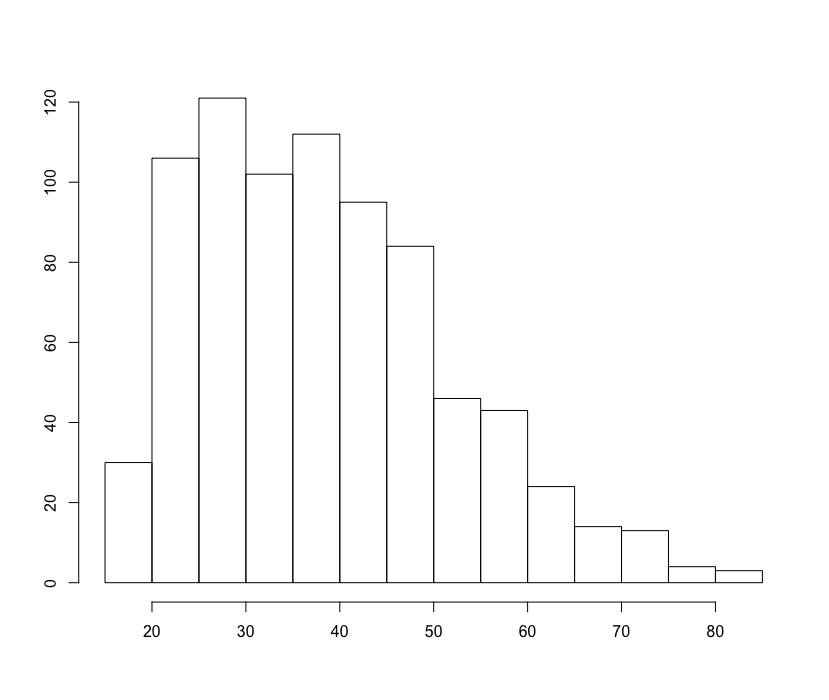
\includegraphics[scale=0.4]{ilu/cd.png}\end{center}\end{figure}
Nous pouvons � pr�sent nous poser la question de la \textit{Normalit�} de la distribution. \newline
\\
Certes, le repr�sentation nous montre une allure de courbe en cloche mais n�anmoins assym�trique. Vraisemblablement, l'�ge ne suit pas une loi Normale.\newline
Bien que nous ayons conclu que cette distribution ne suivait pas une loi Normale, nous aurions pu, si nous avions 20 sujets par groupe, alors qu'\textit{officiellement}, nous ne pouvons utiliser le test de Student, l'appliquer quand m�me  et celui ci fonctionnerait tr�s bien.\newline
\\
L'analyse graphique d'une distribution n'est pas un crit�re tr�s rigoureux. On peut donc se poser la question de savoir si il existe une r�gle qui permet de dire si une distribution suit une loi Normale et si l'on peut utiliser un test t de Student. La r�ponse est \textbf{non}. Certains statisticiens testeront la normalit� de la variable mais cette pratique ne r�pond pas � la question.\newline
En effet, un test statistique n'est utilisable que si l'on souhait� d�montrer que la variable \underline{ne suit pas une loi normale}, c'est l� le principal int�r�t des tests statistiques. De mani�re g�n�rale, un test statistique ne permettra \textbf{jamais} d'affirmer avec certitude qu'une variable suit une loi Normale. De plus, on sait que l'immense majorit� des variables ne suivent pas r�ellement une loi Normale, cela n'est toujours qu'approximatif.\newline
La vraie question avec le test t de Student est donc \textit{Dans quelle mesure la loi est elle suffisamment normale pour r�aliser un test t de Student} mais les statistiques ne r�pondront jamais � cette question.\newline
\\
Pour essayer d'apporter \textit{une r�ponse plus rigoureuse � la question de la normalit� d'une variable}, les statisticiens proposent de r�aliser un \textbf{diagramme de normalit�}.\newline
Avec \textbf{R}, pour obtenir un tel diagramme, il faut utiliser les fonctions \textit{qqnorm} et \textit{qqline}.

\begin{lstlisting}[language=html]
qqnorm(smp.c$age)
qqline(smp.c$age)
\end{lstlisting}
\begin{figure}[H]\begin{center}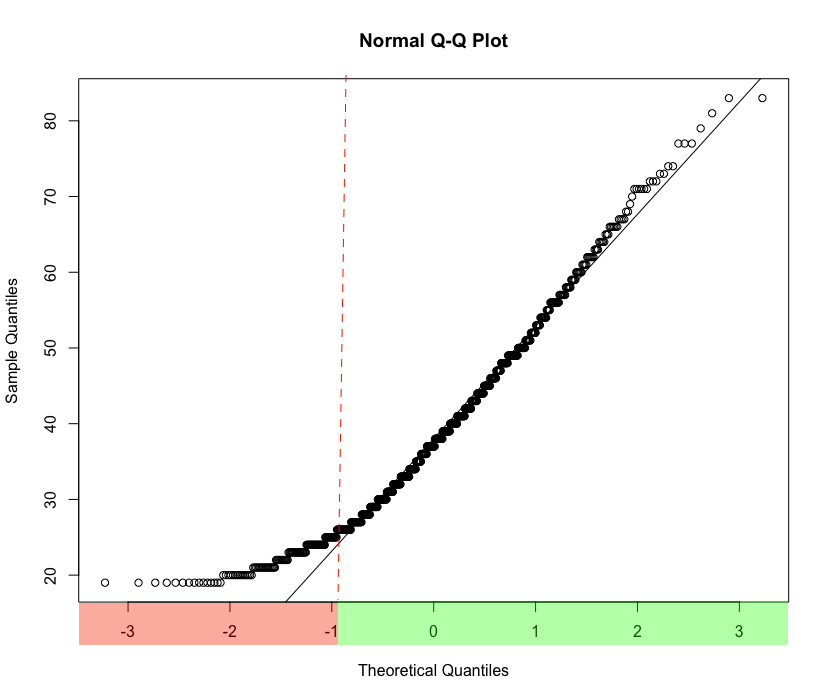
\includegraphics[scale=0.5]{ilu/ce.png}\end{center}\end{figure}
On obtient alors une s�rie de points qui sont normalement tous align�s. On voit ici que c'est le cas pour le milieu de la distribution et sa partie droite. Par contre, pour la partie gauche de la distribution, on peut observer que les points s'�cartent de la ligne. \textbf{On a donc localement, un �cart � la normalit�}.\newline
Les statisticiens dignes de ce nom pensent que cette approche est pr�f�rable.\newline
\\
\textbf{Note : } Les deux approches (visualisation de l'histogramme ou du diagramme de normalit�) sont valables et leur utilisation varie d'un statisticien � un autre.\newline
\\
\textbf{La normalit� n'est pas le seul facteur � prendre en compte.}\newline
\\
En effet, le test t de Student impose �galement, comme condition de validit�, que les variances soient identiques dans les groupes que nous devons comparer.\newline
Il faut donc calculer la variance (ou l'�cart type au carr�) selon que les individus pr�sentent un niveau �lev� (1) ou "normal/faible" (0) d'�vitement du danger. \newline
Pour ce faire, nous allons utiliser la fonction \textit{by(variable � �tudier, variable qui d�termine les sous groupes, fonction que l'on souhaite calculer, le mode de gestion des donn�es manquantes)}.\newline
\\
V�rifions d'abord la relation entre l'�cart type et la variance : $\sigma^{2}_{x}=V_{x}$ : 
\begin{lstlisting}[language=html]
> ##Afichage des effectifs par modalit�
> table(smp.c$age)

19 20 21 22 23 24 25 26 27 28 29 30 31 32 33 34 35 36 37 38 39 40 41 42 43 
15 15 18 13 23 30 22 30 25 21 20 25 18 22 26 20 16 18 25 24 23 22 23 19 17 
44 45 46 47 48 49 50 51 52 53 54 55 56 57 58 59 60 61 62 63 64 65 66 67 68 
19 17 16 12 17 23 16 11 10  8 11  6 14  9  7  6  7  5  7  4  5  3  6  4  2 
69 70 71 72 73 74 77 79 81 83 1  1  6  3  2  2  3  1  1  2 
> ##Calcul de la variance
> v<-var(table(smp.c$age))
> v
[1] 73.63023
> ##Calcul de l'�cart type
> s<-sd(table(smp.c$age))
> s
[1] 8.580806
> ##V�rification s^2=v (arondi � deux d�cimales)
> (round(s^2,2))==(round(v,2))
[1] TRUE
\end{lstlisting}
Puisque la relation est v�rifi�, nous allons prendre, au choix, l'�cart tupe pour r�aliser le calcul permettant d'�tudier la condition de validit� d'un test t de Student : 
\begin{lstlisting}[language=html]
> by(smp.c$age,smp.c$ed.bin,sd,na.rm=TRUE)
smp.c$ed.bin: 0
[1] 13.38593
-------------------------------------------------------- 
smp.c$ed.bin: 1
[1] 13.29636
\end{lstlisting}
R�alisons le m�me calcul pour la variance : 
\begin{lstlisting}[language=html]
> by(smp.c$age,smp.c$ed.bin,var,na.rm=TRUE)
smp.c$ed.bin: 0
[1] 179.1831
-------------------------------------------------------- 
smp.c$ed.bin: 1
[1] 176.7933
\end{lstlisting}
Nous pouvons voir que les r�sultats sont approxivement identiques.\newline
\\
\textbf{Convention : } En statistique, on consid�re que lorsqu'un �cart type est sup�rieur � $1,5$ fois l'autre �cart type, les deux �cart types sont diff�rents.
\begin{lstlisting}[language=html]
> x = 13.38593
> y = 13.29636
> (x>=(y)*(1.5))
[1] FALSE
\end{lstlisting}
On peut donc conclure sur l'�galit� des deux �cart-types.\newline
\\
Maintenant que nous avons d�montrer les condition de validit� pour effectuer un test t de Student, nous allons pouvoir le calculer.\newline
Pour ce faire, nous allons utiliser la fonction \textit{test.t(variable � �tudier $\sim$ variable qui d�termine les sous groupes, var.equal = TRUE)}.\newline
Nous utilisons le dernier param�tre car sinon, par d�faut \textbf{R} utilise l'approximation de Welch, qui permet d'avoir un test t de Student m�me quand les variances sont in�gales ce qui n'est pas recommand�.
\begin{lstlisting}[language=html]
> t.test(smp.c$age~ smp.c$ed.bin, var.equal = TRUE)

	Two Sample t-test

data:  smp.c$age by smp.c$ed.bin
t = 1.7142, df = 690, p-value = 0.08694
alternative hypothesis: true difference in means is not equal to 0
95 percent confidence interval:
 -0.2710524  4.0005138
sample estimates:
mean in group 0 mean in group 1 
       39.46383        37.59910 
\end{lstlisting}
Comme nous pouvons le constater, la valeur du $p$ est �gale � $p0.08694$ donc sup�rieur � $0,05$ soit $5\%$. On peut donc pas conclure sur le fait qu'il existe une diff�rence statistiquement significative d'�ge, entre les d�tenus qui ont un niveau �lev� d'�vitement du danger et les d�tenus qui ont un niveau normal ou faible d'�vitement du danger.\newline
la fonction \textit{t.test()} donne �galement les moyennes des �ges en fonction des deux groupes. Nous constatons curieusement que dans le groupe "normal ou faible" d'�vitement du danger, la moyenne d'�ge est de $39$ ans contre $37,5$ ans dans le groupe "�lev�". Au d�but de cette �tude, nous avions suppos� le contraire � savoir \textit{avec l'�ge, le niveau d'�vitement du danger est sup�rieure}, ce qui n'est pas le cas vu les r�sultats que nous venons d'obtenir.\newline
La diff�rence entre les �ges n'est n�anmoins pas significative.\newline
\\
Si nous ne pouvons pas utiliser le test t de Student parce qu'� la fois, nous avons un petit effectif et une variable qui ne suis pas la loi Normale, il est possible d'utiliser le test de \textbf{Mann-Whitney ou de Wilcoxon}.\newline
La fonction \textbf{R} correspondante est la fonction \textit{wilcox.test()} et la syntaxe est tr�s similaire � celle du \textit{t.test()}. Les r�sultats s'interpr�tent de la m�me fa�on.
\begin{lstlisting}[language=html]
> wilcox.test(smp.c$age~smp.c$ed.bin)

	Wilcoxon rank sum test with continuity correction

data:  smp.c$age by smp.c$ed.bin
W = 56770, p-value = 0.06091
alternative hypothesis: true location shift is not equal to 0
\end{lstlisting}
Nous pouvons remarquer que la diff�rence n'est toujours pas significative car nous obtenons un $p$ �gal � environ $6\%$.\newline
\\
En fin de compte, nous pouvons nous demander si le test de Wilcoxon n'est pas une alternative g�n�raliste au test t de Student.\newline
Certains statisticiens pensent que le test de Wilcoxon est un test l�g�rement moins puissant que le test t et donc qu'il est plus pertinent d'utiliser le test t de Student. Cependant, la diff�rence de puissance entre les deux test n'est pas significative. Nous pourrions donc y gagner � utiliser un test qui fonctionne sans pr� conditions.\newline
Cependant, le test de Wilcoxon ne compare pas des moyennes mais des \textbf{rangs d'individus}. On classe les individus et on regarde en moyenne si le rang dans le groupe $A$ est sup�rieur au rang dans le groupe $B$. Dans le chapitre pr�c�dent, nous avons vu qu'interpr�ter une moyenne n'�tait pas une chose ais�e alors que comparer des rangs d'individus devient une m�thode assez abstraite et nous ne sommes pas s�r que tout le monde puisse l'interpr�ter de mani�re appropri�e.\newline
Enfin, si l'on doit avoir recours � un test de Wilcoxon, cela signifie que l'on est sur que la variable ne suit pas une loi Normale et donc de fait, nous ne pourrons pas utiliser d'analyse de variance, de r�gression lin�aire multiple, \dots car ces m�thodes requi�rent une normalit� de variable que l'on utilise.\newline
Le test de Wilcoxon ne permet donc pas de faire des analyses multivari�es ce qui en soit est assez limitatif.
%%%%%%%%%%%%%%%%%%%%%%%%%%%%%%%%%%%%%%%%%%%%%%%%%%%%%%%%%%%%%%%
%%%%%%%%%%%%%%%%%%%%%%%%%%%%%%%%%%%%%%%%%%%%%%%%%%%%%%%%%%%%%%%
%%%%%%%%%%%%%%%%%%%%%%%%%%%%%%%%%%%%%%%%%%%%%%%%%%%%%%%%%%%%%%%
\chapter{Les tests statistiques en pratique : test de la nullit� d'un coefficient de corr�lation, divers}
Le \textbf{Test de nullit� d'un coefficient de corr�lation} ne poss�de pas de nom d�fini comme le test du $\chi^{2}$ ou le test de Student.\newline 
Les conditions de validit� de ce test sont assez simple. Si nous souhaitons tester la nullit� de la corr�lation de la variable $x$ avec la variable $y$, il faut que la \textbf{distribution de $x$ ou celle de $y$ suive une loi Normale}. Il n'est donc pas n�cessaire que les deux variables suivent une loi Normale mais seulement l'une des deux.\newline
\\
Dans le cadre de l'�tude sur la sant� mentale en prison, nous allons �tudier la corr�lation qu'il est susceptible d'avoir entre un �ge �lev� et un niveau de recherche de sensation faible. En effet,  nous allons partir de l'hypoth�se qu'\textit{avec l'�ge, les individus recherchent moins de sensations fortes}.\newline
\\
Nous allons donc tester � $0$ cette corr�lation et la fonction \textbf{R} correspondante est \textit{cor.test()}. la syntaxe est tr�s simple, on met la premi�re variable puis la seconde apr�s une virgule.

\begin{lstlisting}[language=html]
> setwd("~/Desktop/DIVERS_TEMPLATES/R/TP")
> smp.c <-read.csv2("DONNEES/smp1.csv")
> table(smp.c$age,useNA = "always")

  19   20   21   22   23   24   25   26   27   28   29   30   31   32   33 
  15   15   18   13   23   30   22   30   25   21   20   25   18   22   26 
  34   35   36   37   38   39   40   41   42   43   44   45   46   47   48 
  20   16   18   25   24   23   22   23   19   17   19   17   16   12   17 
  49   50   51   52   53   54   55   56   57   58   59   60   61   62   63 
  23   16   11   10    8   11    6   14    9    7    6    7    5    7    4 
  64   65   66   67   68   69   70   71   72   73   74   77   79   81   83 
   5    3    6    4    2    1    1    6    3    2    2    3    1    1    2 
<NA> 
   2 
> table(smp.c$rs,useNA = "always")

   1    2    3 <NA> 
 249  158  289  103 
> cor.test(smp.c$age,smp.c$rs)

	Pearson's product-moment correlation

data:  smp.c$age and smp.c$rs
t = -6.02, df = 694, p-value = 2.825e-09
alternative hypothesis: true correlation is not equal to 0
95 percent confidence interval:
 -0.2922516 -0.1509579
sample estimates:
       cor 
-0.2227744 
\end{lstlisting}
Les r�sultats sont classiques : on obtient $p= 2,825.10^{-9}$, inf�rieur � $10^{-8}$ donc la corr�lation est tr�s significativement non nulle. La fonction cor.test() donne �galement le coefficient de corr�lation qui est ici �gal � $r=-0,2227744$ ce qui confirme notre hypoth�se : \textit{Il y a bien une corr�lation n�gative entre �ge et recherche de sensations}.\newline
La fonction cor.test donne �galement l'intervalle de confiance � $95\%$ de ce coefficient de corr�lation. ce dernier est $[-0,2922516, -0,1509579]$. Il signifie que la corr�lation de $-0,22$ que l'on vient d'observer correspond � la corr�lation des 799 individus. Cet intervalle de confiance permet de r�pondre � la question : \textit{Quelle est la valeur de la corr�lation entre age et recherche de sensation, non pas dans cet �chantillon mais plut�t pour l'ensemble de la population des d�tenus ?} La r�ponse est donc qu'� $95\%$ de chance, la corr�lation se situera dans l'intervalle $[-0,2922516, -0,1509579]$.\newline
\\
Nous avons vu dans le chapitre pr�c�dent que la distribution de l'�ge des d�tenus �tait approximativement Normale mais tr�s asym�trique. Nous pouvons dire que dans le cadre d'une premi�re approximation, la normalit� est suffisante pour accepter d'utiliser le test classique de nullit� d'un coefficient de corr�lation de PEARSON; d'autant plus que la variable \textit{recherche de sensation} ne suit pas du tout une loi normale car c'est une variable qualitative d'�tat prenant comme valeur $1,2$ ou $3$ :
\begin{itemize}
\item 1 - La recherche de sensation est faible 
\item 2 - La recherche de sensation est moyenne 
\item 3 - La recherche de sensation est forte
\end{itemize}
Pour calculer un test de nullit� du coefficient de corr�lation, il faut absolument que la variable �ge suive une loi Normale car sinon, la condition de validit� n'est pas remplie.\newline
Dans le cas o� la pr� condition est viol�, il existe un autre test appel� \textbf{Test de nullit� de la corr�lation de SPEARMAN} et non plus de Pearson.\newline
La corr�lation de SPEARMAN s'int�resse aux rangs des sujets et non plus sur les observations en elles m�mes. Dans notre exemple, nous prenons les �ges des sujets que l'on classe de mani�re croissante et on fait de m�me pour les niveaux de recherche de sensation. On effectue alors le calcul de la corr�lation entre les rangs de l'�ge et ceux de la recherche de sensation. Cette m�thode est consid�r�e comme beaucoup plus robuste.\newline
\\
Pour effectuer le test de corr�lation au sens de SPEARMAN, il suffit d'ajouter \textit{method ="spearman"} � la fonction \textit{cor.test()}.
\begin{lstlisting}[language=html]
> cor.test(smp.c$age,smp.c$rs, method = "spearman")

	Spearman's rank correlation rho

data:  smp.c$age and smp.c$rs
S = 68743000, p-value = 2.567e-09
alternative hypothesis: true rho is not equal to 0
sample estimates:
       rho 
-0.2233474 

Warning message:
In cor.test.default(smp.c$age, smp.c$rs, method = "spearman") :
  Impossible de calculer la p-value exacte avec des ex-aequos
\end{lstlisting}
$p$ vaut alors $2,567.10^{-9}$, toujours consid�r� comme faible, et la corr�lation appel�e ici $\rho$ (rho) est tr�s proche de celle que l'on avait obtenue avec le test de nullit� du coefficient de corr�lation au sens de PEARSON.\newline
\\
A ce stade, il est l�gitime de ce demander l'utilit� du coefficient de corr�lation au sens de PEARSON et de sa condition de normalit� d'une des deux variables alors que SPEARMAN n'impose aucune pr� condition.\newline
\\
Certes, le test de corr�lation de SPEARMAN est un peu moins puissant que celui de PEARSON. Nous avons �galement un autre inconv�nient que l'on peut voir sur les r�sultats de \textbf{R} qui est que les corr�lations de SPEARMAN sont "g�n�es" par les ex-aqueo or ici, l'�tude engendre de nombreux ex-aqueo car le niveau de recherche de sensation est cod� sur trois niveaux. L'impossibilit� de la gestion des ex-aqueo est une limite � l'utilisation de la m�thode de SPEARMAN.\newline
Enfin, de la m�me mani�re qui consiste � r�server le test Wilcoxon � des situations o� la normalit� de la variable n'est pas d�finie, si l'on utilise une corr�lation de SPEARMAN, ce la signifie que de facto, nous allons consid�rer que les variables que l'on souhaite correller ne suivent de loi Normale et donc de fait, cela va nous interdire d'utiliser toute technique statistique qui n�cessite la normalit� de ses variables comme par exemple, une regression lin�aire multiple.\newline
Avant de nous interdire l'utilisation de toutes ces m�thode, nous devons "peser" les pours et les contres et se demander si l'une des variables (et dans notre cas l'�ge) ne suit pas suffisamment une loi Normale, ce qui nous permettrait d'utiliser le coefficient de corr�lation de PEARSON et non celui de SPEARMAN.\newline
\\
Nous allons � pr�sent nous int�resser � des tests statistique qui sont moins fr�quents mais qui sont cependant utiles et que nous nous devons de conna�tre dans le cas o� nous nous retrouverions dans des cas \textit{d�licats}.\newline 
\\
La premi�re de ces situations concerne la \textbf{comparaison d'une moyenne � une moyenne de r�f�rence}.\newline
De mani�re g�n�rale, nous ne connaissons pas la valeur de r�f�rence d'un param�tre dans une population mais dans certain cas, c'est la cas. Prenons l'exemple du QI : Pour un �ge donn�, on sait que la moyenne du QI est �gale � $100$. Dans le cadre d'un groupe de patients hyperactif, on peut �tre amen� � nous demander si la moyenne de leurs QI est conforme � celle de la population de r�f�rence; Il suffit juste de comparer la moyenne du QI de nos patient � 100.\newline
La syntaxe de \textbf{R} dans ces cas est \textit{t.test()} dans laquelle nous indiquons la variable du QI.\newline
Dans la cas suivant, Nous n'avons que les �ges de la population. On pose $\mu = 24 $ (mu). Dans le cas o� nous �tudierions le QI de nos patient avec une moyenne � $100$, on aurait $\mu = 100$.
\begin{lstlisting}[language=html]
> t.test(smp.c$age, mu = 24)

	One Sample t-test

data:  smp.c$age
t = 31.672, df = 796, p-value < 2.2e-16
alternative hypothesis: true mean is not equal to 24
95 percent confidence interval:
 37.97618 39.82307
sample estimates:
mean of x 
 38.89962 
\end{lstlisting}
\textcolor{white}{.}\newline
Le second cas concerne les tests dit \textbf{appari�s}. La plupart des cas o� l'on a recours � des tests appari�s sont des situations dans lesquelles nous avons des mesures dites \textit{avant/apr�s} c'est � dire que l'on �tudie l'�volution d'une population au cours du temps.\newline
On peut discerner deux cas : 
\begin{itemize}
\item \textbf{Cas des variables qualitatives}\newline 
Si nous prenons par exemple l'�tude du niveau de sport des hommes avant et apr�s leurs mariages, nous allons suivre un groupe de $N$ hommes puis nous allons comparer le pourcentage de sportifs avant le mariage au pourcentage de sportifs apr�s le mariage.\newline
Nous pourrions �ventuellement envisager un test du $\chi^{2}$ (comparaison de pourcentages) mais ce dernier\textbf{ne va pas tenir compte de l'�volution} des hommes dans le temps (avant et apr�s le mariage) et que ce sont les m�mes sujets que l'on �tudie en deux temps distincts. En somme, le r�sultat de ce test ne sera pas totalement faux mais il ne prendra	pas en compte le fait que chaque sujet est son propre contr�le.\newline
Pour r�pondre � ce type de probl�me, nous pouvons utiliser le \textbf{test de MACNEMAR}. La fonction \textbf{R} correspondante est \textit{mcnemar.test()} et l'on y indique en param�tre les valeurs dites d'avant (b.debut) et d'apr�s (b.fin) et il retourne une valeur de $p$:
 \begin{lstlisting}[language=html]
> b.debut = c(1,3)
> b.fin = c(3,2)
> mcnemar.test(b.debut,b.fin)

	McNemar's Chi-squared test

data:  b.debut and b.fin
McNemar's chi-squared = 0, df = 1, p-value = 1

> data <- matrix(c(1, 4, 2, 3), ncol=2, byrow=T)
> data
     [,1] [,2]
[1,]    1    4
[2,]    2    3
> mcnemar.test(data)

	McNemar's Chi-squared test with continuity correction

data:  data
McNemar's chi-squared = 0.16667, df = 1, p-value = 0.6831

> data <- matrix(c(25, 5, 15, 15), ncol=2, byrow=T)
> data2 <- matrix(c(16, 11, 3, 21, 8, 1), ncol=2, byrow=T)
> mcnemar.test(data)

	McNemar's Chi-squared test with continuity correction

data:  data
McNemar's chi-squared = 4.05, df = 1, p-value = 0.04417

> chisq.test(data)

	Pearson's Chi-squared test with Yates' continuity correction

data:  data
X-squared = 6.075, df = 1, p-value = 0.01371

> mcnemar.test(data2)
Error in mcnemar.test(data2) : 
  'x' doit �tre carr�e avec au moins deux lignes et deux colonnes
> chisq.test(data2)

	Pearson's Chi-squared test

data:  data2
X-squared = 19.465, df = 2, p-value = 5.932e-05

Warning message:
In chisq.test(data2) : l'approximation du Chi-2 est peut-�tre incorrecte
\end{lstlisting}


\item \textbf{Cas des variables quantitatives}\newline
Cas beaucoup plus fr�quent des test appari�s, on l'utilise pour par exemple, suivre l'�volution du QI d'un enfant avant et apr�s une technique de r��ducation. On peut �galement comparer les revenus d'individus � 30 et 40 ans. Si nous utilisons un test de STUDENT, nous n'allons pas tenir compte du fait que la population est la m�me aux deux moments (avant/apr�s) de l'�tude et nous serons en situation de sous puissance. Il faut donc utiliser le \textbf{Test de Student aux populations appari�es}.\newline
La fonction \textbf{R} correspondante est \textit{t.test()} dans laquelle on d�finit les valeurs avant et apr�s suivi de l'instruction \textit{paired = TRUE}.

\begin{lstlisting}[language=html]
> x.debut =c(22,24,45,34,67,34)
> x.fin =c(72,94,45,14,63,33)
> t.test(x.debut,x.fin, paired = TRUE)

	Paired t-test

data:  x.debut and x.fin
t = -1.0915, df = 5, p-value = 0.3248
alternative hypothesis: true difference in means is not equal to 0
95 percent confidence interval:
 -53.12252  21.45586
sample estimates:
mean of the differences 
              -15.83333 
\end{lstlisting}
\end{itemize}
%%%%%%%%%%%%%%%%%%%%%%%%%%%%%%%%%%%%%%%%%%%%%%%%%%%%%%%%%%%%%%%
%%%%%%%%%%%%%%%%%%%%%%%%%%%%%%%%%%%%%%%%%%%%%%%%%%%%%%%%%%%%%%%
%%%%%%%%%%%%%%%%%%%%%%%%%%%%%%%%%%%%%%%%%%%%%%%%%%%%%%%%%%%%%%%
\chapter{R�gression lin�aire "simple"}
Nous allons � pr�sent commencer une s�rie de chapitres sur la r�gression lin�aire et l'analyse de variances en d�butant par le \textbf{cas particulier de la r�gression lin�aire simple}.\newline
\\
A ce stade, nous allons avoir besoin d'une version du fichier \textit{sant� mentale en prison} plus compl�te. Ce nouveau fichier s'appelle \textit{smp.2.csv} et contient toujours $26$ variables sur $799$ sujets.\newline
\begin{lstlisting}[language=html]
> setwd("~/Desktop/DIVERS_TEMPLATES/R/TP")
> smp <- read.csv2("DONNEES/smp2.csv")
> str(smp)
'data.frame':	799 obs. of  26 variables:
 $ age         : int  31 49 50 47 23 34 24 52 42 45 ...
 $ prof        : Factor w/ 8 levels "agriculteur",..: 3 NA 7 6 8 6 3 2 6 6 ...
 $ duree       : int  4 NA 5 NA 4 NA NA 5 4 NA ...
 $ discip      : int  0 0 0 0 1 0 0 0 1 0 ...
 $ n.enfant    : int  2 7 2 0 1 3 5 2 1 2 ...
 $ n.fratrie   : int  4 3 2 6 6 2 3 9 12 5 ...
 $ ecole       : int  1 2 2 1 1 2 1 2 1 2 ...
 $ separation  : int  0 1 0 1 1 0 1 0 1 0 ...
 $ juge.enfant : int  0 0 0 0 NA 0 1 0 1 0 ...
 $ place       : int  0 0 0 1 1 0 1 0 0 0 ...
 $ abus        : int  0 0 0 0 0 0 0 0 1 1 ...
 $ grav.cons   : int  1 2 2 1 2 1 5 1 5 5 ...
 $ dep.cons    : int  0 0 0 0 1 0 1 0 1 0 ...
 $ ago.cons    : int  1 0 0 0 0 0 0 0 0 0 ...
 $ ptsd.cons   : int  0 0 0 0 0 0 0 0 0 0 ...
 $ alc.cons    : int  0 0 0 0 0 0 0 0 1 1 ...
 $ subst.cons  : int  0 0 0 0 0 0 1 0 1 0 ...
 $ scz.cons    : int  0 0 0 0 0 0 0 0 0 0 ...
 $ char        : int  1 1 1 1 1 1 1 1 4 1 ...
 $ rs          : int  2 2 2 2 2 1 3 2 3 2 ...
 $ ed          : int  1 2 3 2 2 2 3 2 3 2 ...
 $ dr          : int  1 1 2 2 2 1 2 2 1 2 ...
 $ suicide.s   : int  0 0 0 1 0 0 3 0 4 0 ...
 $ suicide.hr  : int  0 0 0 0 0 0 1 0 1 0 ...
 $ suicide.past: int  0 0 0 0 1 0 1 0 1 0 ...
 $ dur.interv  : int  NA 70 NA 105 NA NA 105 84 78 60 ...
\end{lstlisting}
Nous retrouvons les variables suivantes : 
\begin{itemize}
\item \textit{age} : l'�ge des d�tenus 
\item \textit{prof} : la profession des d�tenus  
\item \textit{duree} : la dur�e de la d�tention d'un individu  
\item \textit{discip} : Est ce que le d�tenu est sous mesure disciplinaire  
\item \textit{n.enfant} : Le nombre d'enfant
\item \textit{n.fraterie} : La taille de la fraterie du d�tenu 
\item \textit{ecole} : la variable relative � la scolarisation du d�tenu (comprise entre $1$ et $5$) 
\item \textit{separation} : Est ce que le d�tenu a �t� s�par� de sa famille lorsqu'il �tait enfant (\textit{oui} ou \textit{non})
\item \textit{juge.enfant} : Est ce que le d�tenu a b�n�ficier de l'aide d'un juge pour enfant lorsqu'il �tait enfant  
\item \textit{place} : Est ce que le d�tenu a �t� plac� lorsqu'il �tait enfant 
\item \textit{abus} : Est ce que le d�tenu a �t� victime d'abus 
\end{itemize}
Nous retrouvons �galement les variables de diagnostic :
\begin{itemize}
\item \textit{grav.cons} : La gravit� consensuelle de la maladie du d�tenu
\item \textit{dep.cons} : L'existence d'une d�pression chez le d�tenu  
\item \textit{ago.cons} : L'existence d'un trouble agoraphobique chez le d�tenu  
\item \textit{ptsd.cons} : L'existence d'un syndr�me de stress post - traumatique chez le d�tenu 
\item \textit{alc.cons} : L'existence d'un abus d'alcool chez le d�tenu 
\item \textit{subst.cons} : L'existence d'un abus de susbtance chez le d�tenu 
\item \textit{scs.cons} : L'existence d'un trouble schizophr�nique chez le d�tenu  
\end{itemize}
Et enfin, nous retrouvons les variables de personnalit� suivantes : 
\begin{itemize}
\item \textit{char} : Variable qui correspnd � un score semi-quantitatif qui �value l'importance et l'intensit� d'un trouble de la personnalit� sous-jacent 
\item \textit{rs} : Le niveau de recherche de sensations chez un d�tenu
\item \textit{ed} : Le niveau d'�vitemment du risque chez un d�tenu
\item \textit{dr} : Le niveau de d�pendance � la r�compense chez un d�tenu
\item \textit{suicide.s} : Le score de risque suicidaire d'un d�tenu
\item \textit{suicide.hr} : L'existence d'un haut risque suicidaire - Binarisation de la variable \textit{suicide.s} 
\item \textit{suicide.past} : L'existence d'ant�c�dents de tentative de suicide chez un patient 
\item \textit{dur.interv} : La dur�e de l'entretien que les enqu�teurs ont pass�e avec le d�tenu 
\end{itemize}
Dans notre cursus secondaire, nous avons �tudier des droites de regressions, tr�s pris�es par la communaut� des physiciens.\newline
Dans le cas o� nous avons un nuage de point dans le plan, \textbf{la droite de regression est la droite qui passe, aux mieux, par l'ensemble des points}.
\begin{figure}[H]\begin{center}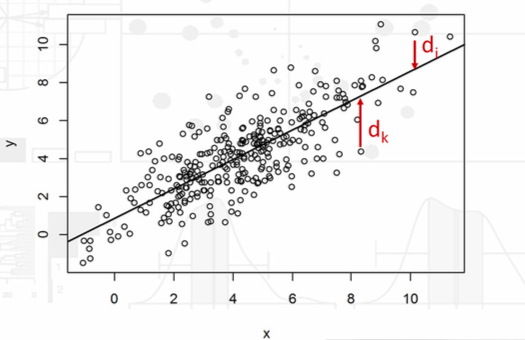
\includegraphics[scale=0.7]{ilu/cl.png}\end{center}\end{figure}
Formellement, la d�finition math�matique de la droite de r�gression correspond, pour tout point $i$, au projet� de ce point, parall�lement � l'axe des ordonn�es, sur la droite de r�gression (comme sur le graphique ci dessus) et on appellera $d_{i}$, la distance entre le point $i$ et sa projection sur la droite.\newline
La d�finition de la droite de r�gression est la droite qui minimise la somme des distances $d_{i}$ entre le point et sa projection sur sa droite, c'est � dire : 
$$\textrm{argmin} (d_{1}^{2}+ \dots + d_{n}^{2}) =  \textrm{argmin} (\sum_{k=1}^{n}d_{k}^{2})$$
Il est donc tr�s facile de repr�senter graphiquement et de calculer une droite de r�gression lin�aire avec \textbf{R}.\newline
Nous allons repr�senter la droite de r�gression lin�aire avec pour valeur de $x$, l'�ge des d�tenus et pour $y$, la dur�e des entretiens que les enqu�teurs ont pass� avec les d�tenus.\newline
Dans un premier temps, on repr�sente le diagramme $x/y$, c'est � dire les �ges en fonction de la dur�e des entretiens gr�ce � la fonction \textit{plot()} :
\begin{lstlisting}[language=html]
plot(smp$age,smp$dur.interv) 
\end{lstlisting}
\begin{figure}[H]\begin{center}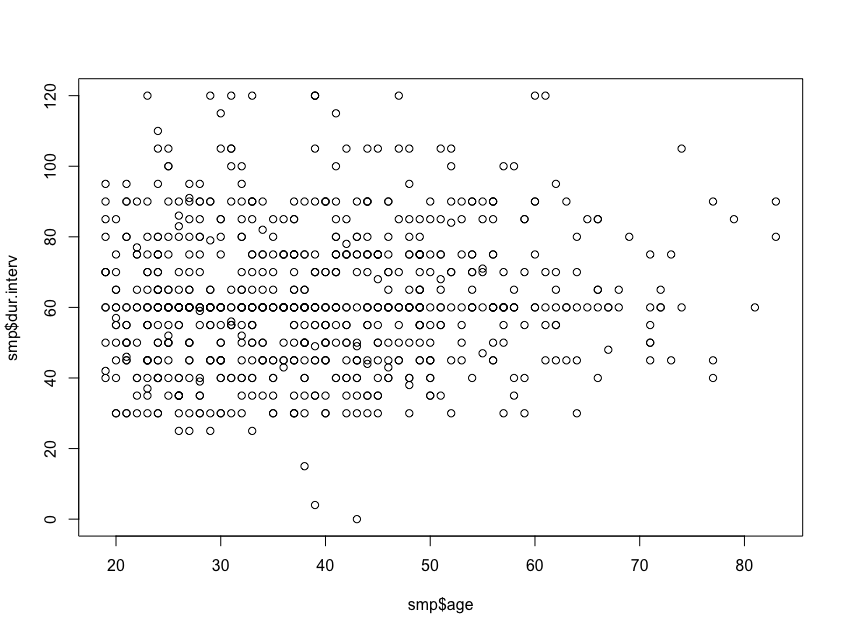
\includegraphics[scale=0.35]{ilu/cm.png}\end{center}\end{figure}
Certes, le graphique est int�ressant; Cependant, nous pouvons voir que les valeurs pour les $799$ ne sont pas repr�sent�es (comme les variables sont discr�tes, les points sont superpos�s les uns sur les autres dans le cas d'une m�me observation). Pour rem�dier � ce probl�me, nous pouvons utiliser la fonction \textit{jitter()}
\begin{lstlisting}[language=html]
plot(jitter(smp$age),jitter(smp$dur.interv))
\end{lstlisting}
\begin{figure}[H]\begin{center}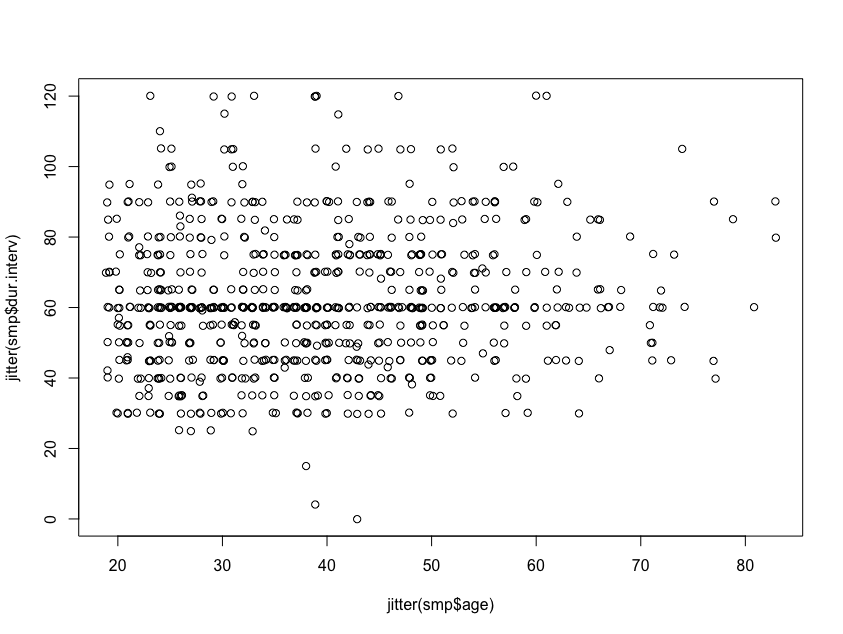
\includegraphics[scale=0.35]{ilu/cn.png}\end{center}\end{figure}
Le graphique obtenu de la sorte est d�j� plus informatif.\newline
Cependant, nous pouvons avoir l'impression que le niveau de \textit{bruit} que le logiciel met par d�faut sur les valeurs des �ges et sur la dur�e des entretiens est trop petit et que l'on observe encore des points superpos�s. Il faut savoir qu'il est possible de modifier \underline{� volont�} l'importance du bruit dans la fonction \textit{jitter()} en ajoutant l'attribut \textit{factor = }.\newline
Pour une valeur de \textit{factor} �gale � 4, on obtient : 
\begin{lstlisting}[language=html]
plot(jitter(smp$age),jitter(smp$dur.interv,factor=4))
\end{lstlisting}
\begin{figure}[H]\begin{center}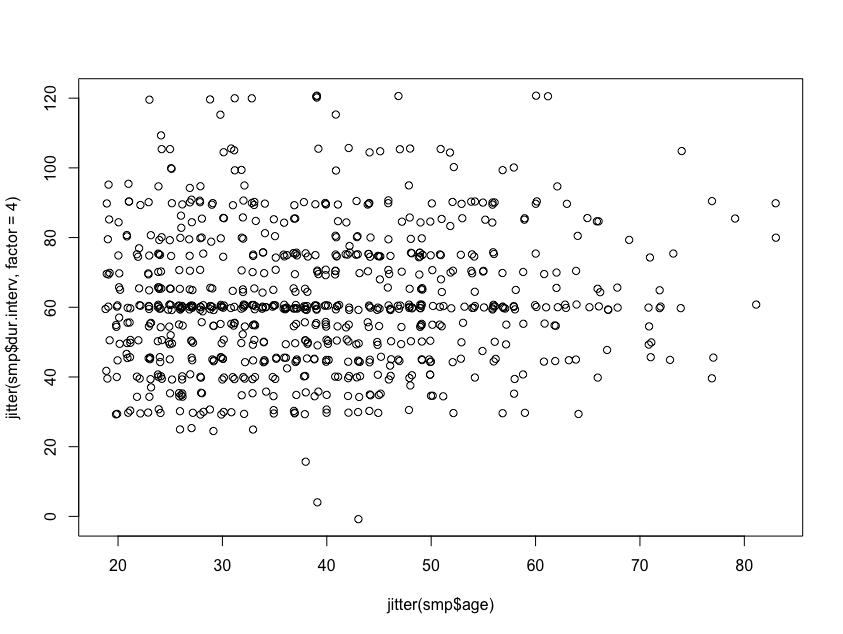
\includegraphics[scale=0.35]{ilu/co.png}\end{center}\end{figure}
Pour une valeur de \textit{factor} �gale � 8, on obtient : 
\begin{figure}[H]\begin{center}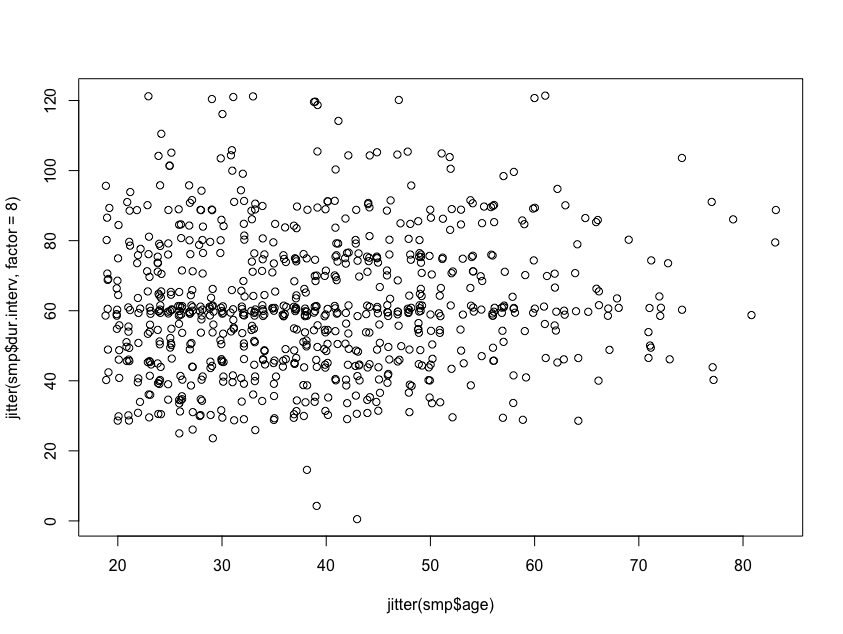
\includegraphics[scale=0.35]{ilu/cp.png}\end{center}\end{figure}
Pour une valeur de \textit{factor} �gale � 64, on obtient : 
\begin{figure}[H]\begin{center}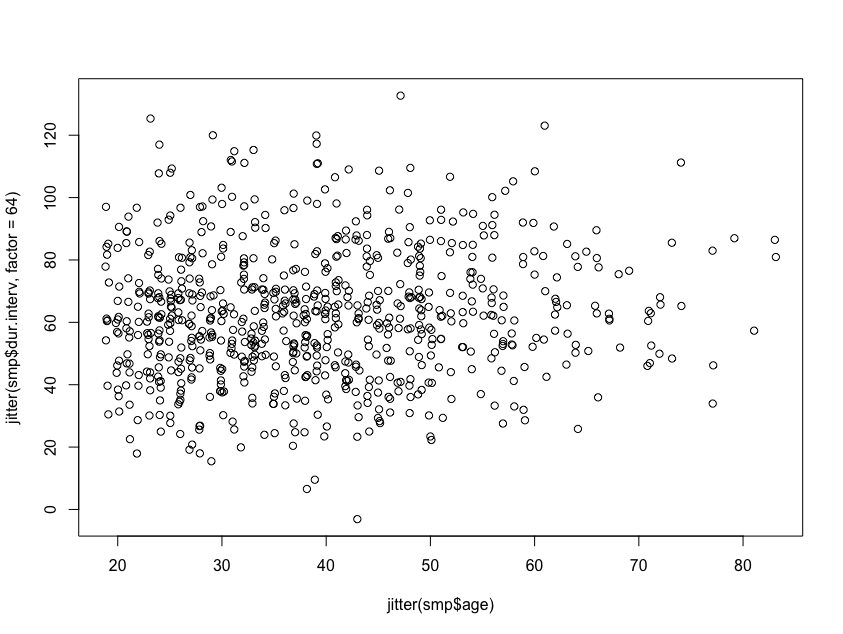
\includegraphics[scale=0.35]{ilu/cq.png}\end{center}\end{figure}
Pour une valeur de \textit{factor} �gale � 64, on obtient : 
\begin{figure}[H]\begin{center}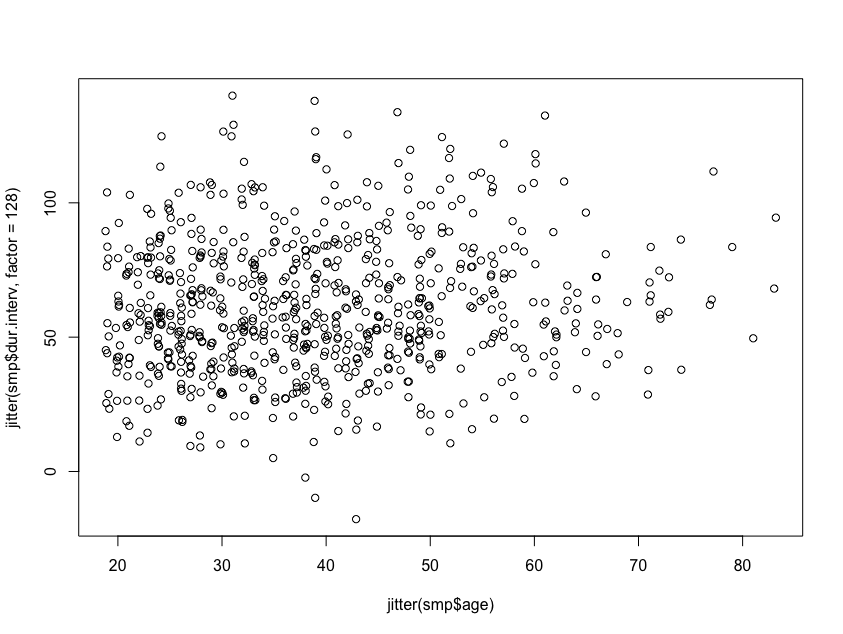
\includegraphics[scale=0.35]{ilu/cr.png}\end{center}\end{figure}
Reprenons le graphique obtenu pour une valeur de \textit{factor} �gale � 4.\newline
\\
Pour tracer une droite de r�gression lin�aire sur un nuage de points, nous devons utiliser la double fonction \textit{abline(lm())} : 
\begin{itemize}
\item La fonction \textit{lm()} permet de calculer les coordonn�es de la droite de r�gression lin�aire, les coefficients $a$ et $b$ pour une droite d'�quation de la forme : 
$$y= b\times x + a$$
\item la fonction \textit{abline()} permet de tracer la droite de r�gression lin�aire 
\item l'attribut \textit{lwd = 2} permet de pr�ciser l'�paisseur de la droite de r�gression sur le graphique.
\end{itemize}

\begin{lstlisting}[language=html]
abline(lm(smp$dur.interv~smp$age),lwd=2)
\end{lstlisting}	
\begin{figure}[H]\begin{center}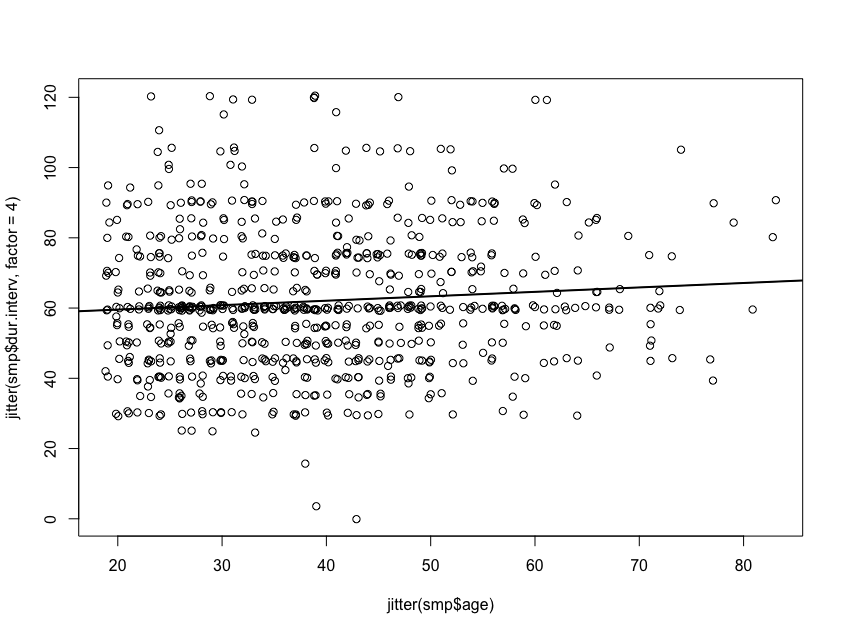
\includegraphics[scale=0.35]{ilu/cs.png}\end{center}\end{figure} 
On peut constater que la droite de r�gression est quasiment parall�le � l'axe des abscisses mais croissante. \newline
La question que nous pouvons nous poser est alors : \textit{La droite de r�gression lin�aire est elle r�ellement croissante ou parall�le � l'axe des abscisses ?}\newline
\\
Pour r�pondre � cette question, ce qui revient � savoir si le coefficient $b$ est statistiquement diff�rent de $0$, nous allons devoir �tudier non pas la droite de r�gression lin�aire mais plut�t \textbf{le mod�le de r�gression lin�aire}.\newline
\\
La diff�rence entre les deux notions vient du fait que dans le mod�le, on prend en compte une \textbf{fonction de bruit} que l'on ajoute � la forme g�n�rale $y =b\cdot x + a$.\newline On consid�re que cette fonction de bruit va suivre une \textbf{Loi Normale}. Gr�ce � cela, il va nous �tre possible de savoir si, statistiquement, $b = 0$ � l'aide d'un test de $p-value$ et comparer ce dernier au risque $\alpha$ de $5\%$.\newline
\\
La fonction du logiciel \textbf{R} qui permet d'estimer un mod�le de r�gression lin�aire est �galement la fonction \textit{lm()} que l'on a utilis� pr�c�demment (lm pour linear model).\newline
Sa synthaxe a �t� pr�sent�e pr�c�demment : 
\begin{itemize}
\item la variable $y$ repr�sente la dur�e de l'entretien
\item le $\sim$ permet de lier les deux variables que l'on souhaite �tudier (a$\sim$b, b en fonction de a)
\item la variable $x$ repr�sente l'�ge
\item \textit{data=smp} repr�sente l'endroit o� sont stock�es les donn�es
\end{itemize} 
\begin{lstlisting}[language=html]
> mod <- lm(dur.interv~age,data=smp)
> summary(mod)

Call:
lm(formula = dur.interv ~ age, data = smp)

Residuals:
    Min      1Q  Median      3Q     Max 
-62.470 -14.402  -1.712  12.341  60.055 

Coefficients:
            Estimate Std. Error t value Pr(>|t|)    
(Intercept) 57.04091    2.22028  25.691   <2e-16 ***
age          0.12625    0.05375   2.349   0.0191 *  
---
Signif. codes:  0 ?***' 0.001 ?**' 0.01 ?*' 0.05 ?.' 0.1 ? ' 1

Residual standard error: 19.57 on 745 degrees of freedom
  (52 observations deleted due to missingness)
Multiple R-squared:  0.00735,	Adjusted R-squared:  0.006018 
F-statistic: 5.516 on 1 and 745 DF,  p-value: 0.0191
\end{lstlisting}
\textbf{Note : } Dans le cas pr�sent, on pr�f�rera stocker l'ensemble des r�sultats issus de la fonction \textit{lm()} dans une objet. L'op�rateur d'affectation est le m�me qu'en pseudo code algorithmique : \textit{<-}. \newline
Ce choix permet d'estimer le mod�le de r�gression de stocker tous les r�sultats issus de ce mod�le dans un objet et d'appeler apr�s des sous objets de cet objet et ceci, les uns apr�s les autres.\newline
Pour obtenir une vision globale des r�sultats de la fonction \textit{lm()}, on peut utiliser la fonction \textit{summary()} sur l'objet que l'on souhaite �tudier et l'on obtient : 
\begin{itemize}
\item Le coefficient directeur de la droite de r�gression lin�aire $b$ �gal � $0,12$
\item L'ordonn�e � l'origine de la droite de r�gression lin�aire $a$ �gal � $57$ (Nomm� \textit{Intercept})
\end{itemize}
On obtient donc la droite de r�gression lin�aire d'�quation suivante : 
$$y = 0,12\times x + 57$$
On peut interpr�ter ces r�sultats comme le fait qu'� chaque fois qu'un d�tenu prend une ann�e suppl�mentaire, les entretiens qu'il aura avec les enqu�teurs augmenteront en moyenne de $0,12$ minutes.\newline
On peut �galement visualiser la valeur de $p$ qui on le rappelle, permet de savoir si \textit{b est significativement diff�rent de 0}? Le r�sultat obtenu est $p=1,9\%$ soit $p<5\%$. On peut donc en d�duire qu'au risque de $5\%$, la pente de la droite de r�gression lin�aire entre la dur�e de l'entretien et l'�ge est significativement diff�rente de $0$.
%%%%%%%%%%%%%%%%%%%%%%%%%%%%%%%%%%%%%%%%%%%%%%%%%%%%%%%%%%%%%%%
%%%%%%%%%%%%%%%%%%%%%%%%%%%%%%%%%%%%%%%%%%%%%%%%%%%%%%%%%%%%%%%
%%%%%%%%%%%%%%%%%%%%%%%%%%%%%%%%%%%%%%%%%%%%%%%%%%%%%%%%%%%%%%%
\chapter{R�gression Lin�aire : au-del� de la corr�lation et du test t}
Dans ce second chapitre sur la r�gression lin�aire, nous allons voir que cette m�thode statistique comporte comme cas particulier le test de nullit� d'un coefficient de corr�lation ainsi que le test t de STUDENT.\newline
\\
Dans le chapitre pr�c�dent, nous avons estim� un mod�le de r�gression lin�aire simple qui associait la dur�e des entretiens avec l'�ge des d�tenus sous la forme d'une �quation simple de type 
$$y=b\cdot x + a + \textrm{bruit}$$
Nous avons calcul� a puis b, b �tant �gal � $0,12$, c'est � dire proche de $0$. De plus, nous avons test� si $b$ �tait statistiquement diff�rent de $0$ et la valeur de $p$ pour ce test �tait de $1,9\%$, $p<5\%$; Nous en avons donc conclu qu'avec un risque de $5\%$, b est statistiquement diff�rent de $0$.\newline
\\
Nous pouvons donc � pr�sent nous pencher sur l'interpr�tation de la diff�rence de $b$ avec $0$ au sens statistique.\newline
L'interpr�tation naturelle qui d�coule de l'�quation de regression est de dire que lorsque l'�ge du d�tenu augmente, en moyenne, la dur�e de l'entretien r�alis� avec les cliniciens augmente elle aussi (de $0,12$).\newline
Cependant, si nous avions calcul� la corr�lation entre la dur�e de l'entretien et l'�ge du d�tenu et que nous obtenions une corr�lation positive, nos conclusions auraient �t� identiques.\newline
Nous avons donc deux tests statistiques qui testent la m�me hypoth�se exactement. Nous pouvons donc esp�rer que les r�sultats (valeurs de $p$) soient proches. Nous allons donc le v�rifier puis tester la nullit� de la corr�lation entre la dur�e des entretiens et l'�ge.\newline
\\
Nous rappellons les r�sultats obtenus pr�c�demment : 
\begin{lstlisting}[language=html]
> mod <- lm(dur.interv~age,data=smp)
> summary(mod)

Call:
lm(formula = dur.interv ~ age, data = smp)

Residuals:
    Min      1Q  Median      3Q     Max 
-62.470 -14.402  -1.712  12.341  60.055 

Coefficients:
            Estimate Std. Error t value Pr(>|t|)
(Intercept) 57.04091    2.22028  25.691   <2e-16
age          0.12625    0.05375   2.349   0.0191
               
(Intercept) ***
age         *  
---
Signif. codes:  
0 ?***' 0.001 ?**' 0.01 ?*' 0.05 ?.' 0.1 ? ' 1

Residual standard error: 19.57 on 745 degrees of freedom
  (52 observations deleted due to missingness)
Multiple R-squared:  0.00735,	Adjusted R-squared:  0.006018 
F-statistic: 5.516 on 1 and 745 DF,  p-value: 0.0191
\end{lstlisting}
Pour calculer la seconde corr�lation, nous allons utiliser la fonction \textit{cor.test()} : 

\begin{lstlisting}[language=html]
> cor.test(smp$age,smp$dur.interv)

	Pearson's product-moment correlation

data:  smp$age and smp$dur.interv
t = 2.3487, df = 745, p-value = 0.0191
alternative hypothesis: true correlation is not equal to 0
95 percent confidence interval:
 0.01408787 0.15650345
sample estimates:
       cor 
0.08573358 
\end{lstlisting}
Nous pouvons remarquer que dans les deux tests, la valeur de $p$ est �gale � $1,91\%$. La conclusion des test est exactement la m�me � savoir \underline{$b \neq 0$}.\newline
\\
Dans les r�sultats obtenus ci dessus, nous avons une valeur de la corr�lation entre la dur�e des entretiens et l'�ge vaut $0,085$, la valeur du coefficient directeur de la droite de r�gression lin�aire $b=0,12$. On peut donc en conclure qu'il existe une �quation math�matique qui lie ces deux valeurs.\newline
Dans ce cas, la corr�lation est : 
$$r = b \times \frac{\sigma_{\textrm{�ge}}}{\sigma_{\textrm{dur�e entretiens}}}$$

Nous pouvons donc nous demander, puisque les valeurs de $p$ obtenues pour un test de nullit� de la corr�lation et le test $b=0$ sont identiques et qu'il nous est possible de d�duire la valeur de $b$, si il est vraiment pertinent de r�aliser des r�gressions lin�aires simples.\newline 
\begin{lstlisting}[language=html]
> mod <- lm(dur.interv~age,data=smp)
> summary(mod)

Call:
lm(formula = dur.interv ~ age, data = smp)

Residuals:
    Min      1Q  Median      3Q     Max 
-62.470 -14.402  -1.712  12.341  60.055 

Coefficients:
            Estimate Std. Error t value Pr(>|t|)    
(Intercept) 57.04091    2.22028  25.691   <2e-16 ***
age          0.12625    0.05375   2.349   0.0191 *  
---
Signif. codes:  0 ?***' 0.001 ?**' 0.01 ?*' 0.05 ?.' 0.1 ? ' 1

Residual standard error: 19.57 on 745 degrees of freedom
  (52 observations deleted due to missingness)
Multiple R-squared:  0.00735,	Adjusted R-squared:  0.006018 
F-statistic: 5.516 on 1 and 745 DF,  p-value: 0.0191
\end{lstlisting}

En faveur de la r�gression lin�aire simple : comme nous pouvons le voir dans cette portion de code, nous obtenons directement les valeurs de $b$ et de $a$ pour �tablir une r�gression lin�aire simple avec $a=57,04$ et $b=0,126$ d'�quation : 

$$y = 0,126\cdot b + 57,04 + \textrm{bruit}$$

De plus, le $b$ a une interpr�tation concr�te � savoir : \textit{Par rapport � un groupe de d�tenus d'�ge donn�, si l'on analyse les r�sultats pour un autre groupe de d�tenus ayant un an de plus, la dur�e des entretiens augmentent de $0,12$ minutes}. Il serait �galement possible de dire que \textit{par rapport � un groupe de d�tenus qui ont un �ge donn� et un autre groupe qui � 10 ans de plus, l'augmentation de la dur�e des entretiens est de $10\times b$ soit $1,2$ minutes}.\newline
Cependant, nous allons voir � pr�sent que la r�gression lin�aire simple \textbf{englobe plusieurs m�thodes.}\newline
\\
Int�ressons nous maintenant � un nouvel exemple qui peut sembler �trange au premier regard mais le r�sultat final est int�ressant.\newline Nous conservons la m�me variable $y$ � savoir la \textit{dur�e des entretiens} mais pour la variable $x$, nous prenons � pr�sent la \underline{variable qualitative binaire} \textit{D�pression consensuelle} (absence (0) ou pr�sence (1) de d�pression). Nous allons � pr�sent en faire une repr�sentation graphique : 
\begin{lstlisting}[language=html]
> table(smp$dep.cons)

  0   1 
482 317 
> plot(jitter(smp$dep.cons,factor=1),jitter(smp$dur.interv,factor=4))
> abline(lm(smp$dur.interv~smp$dep.cons),lwd=2,col="red")
\end{lstlisting}
\begin{figure}[H]\begin{center}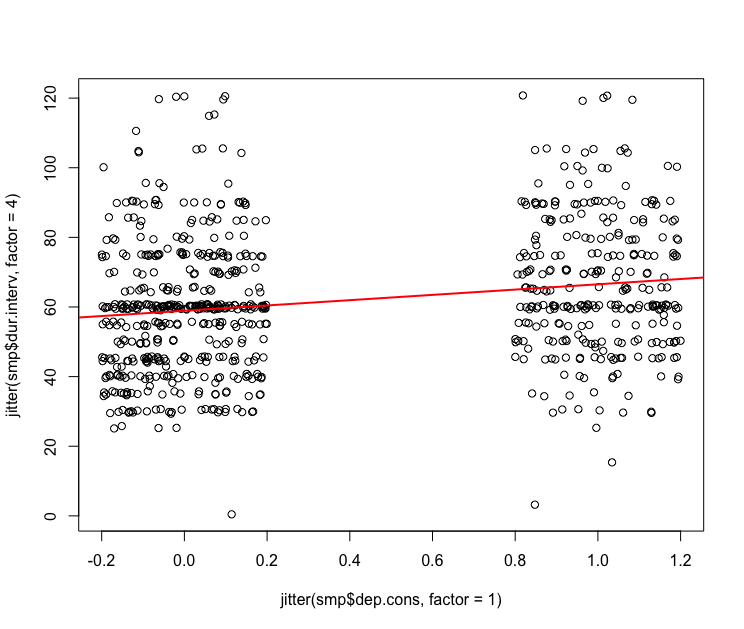
\includegraphics[scale=0.5]{ilu/ct.png}\end{center}\end{figure}
Nous avons donc estim� le mod�le de regression suivant : 

$$ y = a + b\times x, b \neq 0$$ 
O� $x$ correspond � la pr�sence de d�pression et $y$, la dur�e des entretiens. Nous reviendrons plus tard sur les conditions de validit� pour l'application du mod�le de r�gression lin�aire simple.\newline 
\\
Traditionellement, $b$ repr�sente le facteur qui \textit{lorsque la variable de d�pression augmente d'un point, alors la variable augmente de $b$ points} comme nous l'avons vu dans l'exemple pr�c�dent.\newline
Dans ce cas, lorque la variable depression augmente d'un point, alors nous passons d'absence d'�tat d�pressif � pr�sence de ce dernier.\newline 
Donc la variation correspondante de dur�e est en fait �gale � la variation de dur�e des entretiens entre les groupes des d�tenus pr�sentant une symptomatologie d�pressive et ceux n'en pr�sentant pas.\newline 
On peut cependant se poser la question concernant la valeur de $b$; Si cette derni�re correspond � la diff�rence de dur�e des entretiens entre les deux types de d�tenus, si nous testons $b\neq 0$, alors nous devrions th�oriquement obtenir les m�mes dur�es pour chaque d�tenu, comme si nous utilisions un test t de STUDENT qui comparent la moyenne des dur�es d'entretien entre les d�tenus d�pressifs et ceux non d�pressifs.\newline
\begin{lstlisting}[language=html]
> mod <- lm(dur.interv~dep.cons,data = smp)
> summary(mod)

Call:
lm(formula = dur.interv ~ dep.cons, data = smp)

Residuals:
    Min      1Q  Median      3Q     Max 
-62.538 -13.923   1.077  12.077  61.077 

Coefficients:
            Estimate Std. Error t value Pr(>|t|)    
(Intercept)  58.9234     0.9041  65.171  < 2e-16 ***
dep.cons      7.6143     1.4481   5.258  1.9e-07 ***
---
Signif. codes:  0 ?***' 0.001 ?**' 0.01 ?*' 0.05 ?.' 0.1 ? ' 1

Residual standard error: 19.33 on 747 degrees of freedom
  (50 observations deleted due to missingness)
Multiple R-squared:  0.03569,	Adjusted R-squared:  0.0344 
F-statistic: 27.65 on 1 and 747 DF,  p-value: 1.9e-07

> t.test(smp$dur.interv~smp$dep.cons, var.equal =TRUE)

	Two Sample t-test

data:  smp$dur.interv by smp$dep.cons
t = -5.2583, df = 747, p-value = 1.9e-07
alternative hypothesis: true difference in means is not equal to 0
95 percent confidence interval:
 -10.457001  -4.771515
sample estimates:
mean in group 0 mean in group 1 
       58.92341        66.53767 
\end{lstlisting}
On peut remarquer que nous obtenons les m�mes valeurs de $p$ mais �galement, que la diff�rence des moyennes entre les deux groupes obtenues avec la fonction \textit{t.test()} retourne une valeur �gale � celle de $b$ ($b = 7.6143$ et $|58.9234-66.53767| = 7.61427$).\newline
Nous pouvons donc conclure que r�aliser un mod�le de r�gression lin�aire simple (dur�e de l'entretien en fonction de la pr�sence d'une symptomatologie d�pressive) retourne des r�sultats identiques � ceux obtenues par comparaison des moyennes dans le cadre du test t.\newline
Nous avions vu pr�c�demment que la r�gression lin�aire simple �tait une \textbf{g�n�ralisation du test de nullit� d'un coefficient de corr�lation}, nous pouvons maintenant affirmer que la r�gression lin�aire est �galement une \textbf{g�n�ralisation du test t de STUDENT}.

%%%%%%%%%%%%%%%%%%%%%%%%%%%%%%%%%%%%%%%%%%%%%%%%%%%%%%%%%%%%%%%
%%%%%%%%%%%%%%%%%%%%%%%%%%%%%%%%%%%%%%%%%%%%%%%%%%%%%%%%%%%%%%%
%%%%%%%%%%%%%%%%%%%%%%%%%%%%%%%%%%%%%%%%%%%%%%%%%%%%%%%%%%%%%%%
\chapter{R�gression lin�aire multiple et analyse de variances}

Dans ce chapitre, nous allons nous int�resser aux r�gressions lin�aires multiples et � l'analyse de variances.\newline
Dans le chapitre pr�c�dent, nous avons montr� que la dur�e des entretiens r�alis�s dans l'�tude sant�e mentale en prison �tait associ�e � l'�ge des d�tenus. Nous avons �galement montr� que la dur�e de l'entretien �tait associ�e � l'existence d'un trouble d�pressif. Nous pourrions montrer de la m�me fa�on que cette dur�e d'entretien est li�e � un abus de substances et � l'existence d'un trouble schizophr�nique.\newline
Le probl�me est que ces quatres variables (�ge, depression, abus de substances et trouble schizophr�nique) sont \textit{plus ou moins reli�es les une aux autres}.\newline
Par transitivit�, on peut d�montrer que l'existence d'une d�pression est li�e � l'�ge, l'existence d'une abus de substances est particuli�rement li�e � une symptomatologie d�pressive, \dots.\newline
\\
Nous pouvons nous poser alors les questions suivantes : \textit{Est-ce que la dur�e d'entretien varie en fonction de la d�pression parce que les d�tenus, quand ils sont d�prim�s, consomment des substances voire m�me le contraire, est-ce que la dur�e de l'entretien est li�e � l'abus de substance tout simplement parce que les sujets d�prim�s consomment des substances et quand ils sont d�prim�s, ils mettent plus longtemps � r�pondre ?} \dots 
Comment peut on trouver un sens commun dans tout ce r�seau de relations et analyser au mieux les patterns\footnote{Le mot anglais � pattern � est souvent utilis� pour d�signer un mod�le, une structure, un motif, un type, \dots. Il s'agit souvent d'un ph�nom�ne ou d'une organisation que l'on peut observer de fa�on r�p�t�e lors de l'�tude de certains sujets, auquel il peut conf�rer des propri�t�s caract�ristiques. } d�finis autour de la variable qui nous int�resse : \textbf{dur�e des entretiens} avec les variables explicatives \textbf{�ge, depression, abus de substances, \dots}\newline
\\
Dans le chapitre pr�c�dent, nous avons utiliser le mod�le de r�gression lin�aire suivant pour montrer la relation entre la dur�e des entretiens et l'�ge :
$$ y_{0} = a + b\times x + \textrm{bruit}_{0}, \textrm{ avec } x = \textrm{ l'�ge et } y = \textrm{ la dur�e.}$$
De la m�me fa�on, nous pouvons �tablir des mod�les quasi identiques pour repr�senter les diff�rentes relations :
$$ y_{1} = a + c\times x + \textrm{bruit}_{1}, \textrm{ avec } x = \textrm{ d�pression et } y = \textrm{ la dur�e.}$$
$$ y_{2} = a +d\times x + \textrm{bruit}_{2}, \textrm{ avec } x = \textrm{ substances et } y = \textrm{ la dur�e.}$$
$$ y_{3} = a +e\times x + \textrm{bruit}_{3}, \textrm{ avec } x = \textrm{ schizophr�nie et } y = \textrm{ la dur�e.}$$
Nous pouvons tenter d'expliquer la variation de la dur�e d'entretiens gr�ce aux $4$ variables explicatives en combinant ces $4$ syst�mes avec $a$, un coefficient unique calcul� une seule fois et en consid�rant 
$$\textrm{bruit}_{T} = \sum_{i=0}^{n} \textrm{bruit}_{i}\textrm{ avec } n \textrm{le nombre de variables explicatives.}$$
Nous obtiendrons donc le mod�le de regression lin�aire multiple suivant : 
$$ y_{T} = a + b\times x + c\times x + d\times x + e\times x + \textrm{bruit}_{T} $$ 
\textit{b,c,d et e sont les coefficient explicit� dans les syst�mes $y_{i}$}.\newline
\\
Ainsi, nous pouvons d�s lors montrer de mani�re tr�s simple qu'� partir de ce mod�le, les test de nullit� du coefficient de corr�lation $b=0$ revient � tester l'hypoth�se \textit{Est ce que la dur�e de l'entretien est impact�e par l'�ge du d�tenu} ceteris paribus\footnote{Toutes choses �gales par ailleurs : Expression utilis�e pour signifier qu?on laisse de c�t� un certain nombre de param�tres d?une situation donn�e pour n?en �tudier qu?un seul � la fois.} c'est � dire � niveaux de d�pression, d'abus de substances et de schizophr�nie consid�r�s comme constants.\newline 
Il est �galement possible de d�montrer que l'interpr�tation du coefficient de corr�lation $b$ peut maintenant avoir comme signification : \textit{De combien augmente la dur�e de l'entretien quand l'�ge augmente d'un an � d�pr�ssion, abus de substances et schizophr�nie constants ?}\newline 
On dit parfois que le coefficient $b$ caract�rise l'association entre la dur�e de l'entretien et l'�ge avec ajustement sur d�pression, consommation de substances et schizophr�nie.\newline 
\\
Le mod�le pr�c�dent est souvent appel� \textbf{mod�le de regression lin�aire multiple}, multiple car on consid�re plusieurs variables explicatives. La fonction \textbf{R} qui permet de r�aliser des r�gressions lin�aires multiple est la fonction \textit{lm()}. La syntaxe utilis�e est tr�s proche de celle que l'on a mis en oeuvre dans le cas d'une r�gression lin�aire simple : 
\begin{center}
\textit{lm(variable �tudi� $\sim$ variable explicative 1 + variable explicative 2 + \dots }
\end{center}

\begin{lstlisting}[language=html]
> mod_reg_mul <- lm(dur.interv~age+dep.cons+subst.cons+scz.cons,data = smp)
> summary(mod_reg_mul)
Call:
lm(formula = dur.interv ~ age + dep.cons + subst.cons + scz.cons, 
    data = smp)

Residuals:
    Min      1Q  Median      3Q     Max 
-63.654 -14.522  -1.193  11.482  62.482 

Coefficients:
            Estimate Std. Error t value Pr(>|t|)    
(Intercept) 48.90105    2.62213  18.649  < 2e-16 ***
age          0.22096    0.05708   3.871 0.000118 ***
dep.cons     7.38932    1.44783   5.104 4.24e-07 ***
subst.cons   5.25157    1.74318   3.013 0.002678 ** 
scz.cons     2.27256    2.52323   0.901 0.368062    
---
Signif. codes:  0 ?***? 0.001 ?**? 0.01 ?*? 0.05 ?.? 0.1 ? ? 1

Residual standard error: 19.1 on 742 degrees of freedom
  (52 observations deleted due to missingness)
Multiple R-squared:  0.05833,	Adjusted R-squared:  0.05325 
F-statistic: 11.49 on 4 and 742 DF,  p-value: 4.692e-09
\end{lstlisting}

Comme dans le cas de la r�gression lin�aire simple, la colonne \textit{Estimate} rassemble les valeurs des diff�rents coefficients : 
\begin{itemize}
\item \textit{(Intercept)} retournant la valeur du coefficient $a$ (dans notre mod�le)
\item \textit{(age)} retournant la valeur du coefficient de r�gression lin�aire $b$ repr�santant l'�ge des d�tenus 
\item \textit{(dep.cons)} retournant la valeur du coefficient de r�gression lin�aire $c$ repr�santant la pr�sence d'une symptomatologie d�pressive chez les d�tenus 
\item \textit{(subst.cons)} retournant la valeur du coefficient de r�gression lin�aire $d$ repr�santant la consommation de substances chez les d�tenus
\item \textit{(dep.cons)} retournant la valeur du coefficient de r�gression lin�aire $e$ repr�santant la pr�sence d'une symptomatologie schizophr�nique chez les d�tenus 
\end{itemize}

On obtient alors une estimation de la dur�e $y$ de la forme : 

$$ y_{T} = 48.9 + 0.22\times x + 7.39\times x + 5.25\times x + 2.27\times x + \textrm{bruit}_{T} $$ 

Si nous nous int�ressons plus pr�cisement au coefficient $c$ correspondant � l'�tat d�pr�ssif d'un d�tenu, nous constatons qu'il est �gal � $7,39$ ce qui signifie qu'un d�tenu d�pressif, par rapport � un d�tenu non d�pressif, ceteris paribus, c'est � dire en oblit�rant les effets de l'�ge, de la consommation de substances et d'une possible schizophr�nie, aura en moyenne $7$ minutes d'entretien suppl�mentaires. Nous pouvons �galement conclure qu'un d�tenu consommant des substances aura $5$ minutes suppl�mentaires et qu'un d�tenu pr�sentant une schizophr�nie aura $2$ minutes suppl�mentaires d'entretien.\newline
Il est �galement possible de conclure sur le fait qu'un d�tenu pr�sentant un �tat d�pressif, un abus de substances passera des entretiens avec $7+5 = 12$ minutes suppl�mentaires par rapport � un sujet qui ne serait ni d�prim� et ne consommant pas de substances.\newline
Nous pouvons naturellement effectuer des test de nullit� des coefficient, par exemple sur $e$ o� la valeur du \textit{p-value} est de $0,37$ soit $37\%$; La conclusion est donc qu'au risque de $5\%$, nous ne pouvons pas conclure sur le fait que l'existence d'un trouble schizophr�nique augmente statistiquement la dur�e d'un entretien.\newline
\\
Dans le mod�le que nous venons d'�tudier, la variable que nous souhaitons expliciter, la dur�e de l'interview est une \underline{variable quantitative}. C'est d'ailleurs  \textbf{une n�cessit� dans un mod�le de regression} que, compte tenu de l'�quation de r�gression elle m�me, la variable � expliquer soit une somme de de variables explicatives et donc une quantit�.\newline
Les variables explicatives sont soit l'�ge, un variable quantitative, soit les variables d�pression, consommation de substances et schizophr�nie qui sont quant � elles, des variables qualitatives binaires. Avec ce type de variables, il est possible de r�pondre � la grande majorit� des cas que l'on peut rencontrer en pratique.\newline
Il existe cependant des situations o� l'on souhaiterait tout de m�me \underline{mettre en variables explicatives, des variables qualitatives de plus de deux classes} comme par exemple, la profession.\newline

$$ y_{T} = a + b\times \textrm{�ge } + c\times \textrm{d�p } + d\times\textrm{subst }  + e\times\textrm{scz } + f\times\textrm{prof } \textrm{bruit}_{T} $$ 
Pour expliquer la dur�e de l'interview par l'�ge, le niveau de d�pression, la consommation de substances, la schizophr�nie consensuelle et la profession, nous pourrions penser � ajouter un nouveau facteur � l'�quation existente : $f\times\textrm{prof }$; Mais cela ne va pas fonctionner.\newline
En effet, la variable \textit{profession} est repr�sent�e par des \underline{cat�gories} (agriculteur, artisan, cadre, \dots) et il nous est impossible de multiplier dans une �quation des coefficients par des mots (LOL).\newline
Nous pourrions �tre tent� de recoder la variable \textit{profession} par des niveaux ($1,2,3,4,4,6,7,8$) avec 1 pour "agriculteur", 2 pour "artisan",\dots . Mais un tel codage serait un pi�ge; En effet, si nous partons du principe que $1$ repr�sente les agriculteurs et que $3$ repr�sente les cadres, en calculant la moyenne des deux niveaux, nous obtenons $2$ qui correspond � la cat�gorie des artisans. Cela signifierai que l'effet de la profession d'artisan serait la moyenne des effets des professions d'agriculteur et de cadre ce qui n'a aucun sens.\newline
Si l'on veut introduire la variable \textit{profession}, alors il faut la recoder en plusieurs variables binaires. Ainsi, puisqu'il y a $8$ modalit�s dans la variable \textit{profession}, alors nous devrons recoder cette variable en $7$ variables binaires.\newline
Un exemple est donn� ci dessous. On suppose une premi�re variable binaire $f_{1}$ dont la valeur sera $1$  si la profession du d�tenu est "artisan" et $0$ sinon. La deuxi�me variable $f_{2}$ vaudra 1 si le m�tier du d�tenu est "cadre", 0 sinon, \dots  jusqu'� "sans profession".\newline
Nous pouvons voir que la variable "agriculteur", est cod�e implicitement. En effet, si $f_{1}, \dots , f_{7}$ sont toutes �gales � $0$, alors la profession du d�tenu sera n�cessairement "agriculteur".\newline
Ce proc�d� de traduction de variables cat�goricielles en variables binaires est automatiquement r�alis� par \textbf{R}.

\begin{lstlisting}[language=html]
> mod_reg_mul <- lm(dur.interv~age+dep.cons+subst.cons+scz.cons+prof,data = smp)
> summary(mod_reg_mul)

Call:
lm(formula = dur.interv ~ age + dep.cons + subst.cons + scz.cons + 
    prof, data = smp)

Residuals:
    Min      1Q  Median      3Q     Max 
-63.280 -14.164  -1.337  10.959  63.184 

Coefficients:
                        Estimate Std. Error t value Pr(>|t|)    
(Intercept)             62.79202   10.20779   6.151 1.26e-09 ***
age                      0.21289    0.05884   3.618 0.000317 ***
dep.cons                 7.36792    1.45840   5.052 5.53e-07 ***
subst.cons               5.34589    1.76902   3.022 0.002599 ** 
scz.cons                 2.50439    2.54734   0.983 0.325863    
profartisan            -11.48515    9.82936  -1.168 0.243005    
profautre              -10.28748   10.33482  -0.995 0.319862    
profcadre              -19.29636   10.38568  -1.858 0.063574 .  
profemploye            -13.55809    9.76340  -1.389 0.165358    
profouvrier            -14.01270    9.72111  -1.441 0.149880    
profprof.intermediaire -13.01926    9.96911  -1.306 0.191977    
profsans emploi        -14.27866    9.71782  -1.469 0.142174    
---
Signif. codes:  0 ?***? 0.001 ?**? 0.01 ?*? 0.05 ?.? 0.1 ? ? 1

Residual standard error: 19.11 on 731 degrees of freedom
  (56 observations deleted due to missingness)
Multiple R-squared:  0.06595,	Adjusted R-squared:  0.05189 
F-statistic: 4.692 on 11 and 731 DF,  p-value: 5.825e-07
\end{lstlisting}

Dans la pratique, nous pouvons voir que nous retrouvons la fonction \textit{lm()} (linear model).\newline
Le d�but de notre syntaxe est identique et nous avons juste ajout� en param�tre de la fonction \textit{lm()}, une variable explicative (et dans notre exemple, la variable correpondant aux professions).\newline
Comme la variable est constitu�e de mots, \textbf{R} reconnait une variable cat�goricielle et va ainsi automatiqiuement recoder la variable profession \textit{en autant de variables binaires qu'il y a de modalit�s moins une}.\newline
\textbf{Attention : } le pi�ge classique est de consid�rer que la variable \textit{profession} aurait pu etre cod�e par des nombres (1,2,3,...,8 avec 9 professions). Si tel avait �t� le cas, \textbf{R} n'aurait pas pu savoir que la variable profession �tait cat�goricielle et, donc si nous avions inclus \textit{prof} dans le mod�le, \textbf{R} aurait consid�r� que cette variable �tait quantitative et il aurait analys� cette variable en consid�rant que "artisan" est la moyenne de cadre et d?agriculteur. \newline
\\
Dans notre cas, \textit{prof} a bien �t� recod�e en 7 variables binaires et d'ailleurs, c'est ce que nous constatons dans le listing des r�sultats obtenus avec la commande \textit{summary(mod$\_$reg$\_$mul)}.\newline
\\
Nous voyons sept lignes ajout�es aux r�sultats que nous avions obtenus pr�c�dement. \newline
En face de la ligne \textit{profartisant} qui correspond � la modalit� \textit{artisan} dans la variable cat�goricielle \textit{profession}, nous obtenons le coefficient $-11,48$. Ce dernier signifie que les artisans en moyenne mettent 11 minutes de moins lors du d�roulement de l'entretien. On peut voir sur la m�me ligne que la valeur de $p$ est de $0,24$ ce qui n'est pas significatif.\newline
Il n'y a donc \textbf{pas de diff�rence significative} entre la dur�e d'entretien des agriculteurs et la dur�e d'entretien des artisans. On peut d'ailleurs remarquer que les r�sultats sont similaires pour l'ensemble des autres cat�gories professionnelles.\newline
Si en moyenne, toutes les autres cat�gories mettent beaucoup moins de temps que les agriculteurs pour r�pondre, cela n'est cependant pas statistiquement significatif.\newline
\\
Dans ce paragraphe, nous avons consid�r� que la modalit� de r�f�rence �tait la profession \textit{agriculteur}. Or, dans ce dataframe, il n'y a seulement que $6$ agriculteurs sur $799$ d�tenus. En fait, \textbf{R} l'a choisi car c'�tait la premi�re par ordre alphab�tique\newline
Nous allons donc voir maintenant comment modifier la modalit� de r�f�rence dans le codage de la variable profession.\newline
\\
\begin{lstlisting}[language=html]
> smp$prof <- relevel(smp$prof,ref="ouvrier")
> mod_reg_mul <- lm(dur.interv~age+dep.cons+subst.cons+scz.cons+prof,data = smp)
> summary(mod_reg_mul)

Call:
lm(formula = dur.interv ~ age + dep.cons + subst.cons + scz.cons + 
    prof, data = smp)

Residuals:
    Min      1Q  Median      3Q     Max 
-63.280 -14.164  -1.337  10.959  63.184 

Coefficients:
                       Estimate Std. Error t value Pr(>|t|)    
(Intercept)            48.77932    2.83938  17.180  < 2e-16 ***
age                     0.21289    0.05884   3.618 0.000317 ***
dep.cons                7.36792    1.45840   5.052 5.53e-07 ***
subst.cons              5.34589    1.76902   3.022 0.002599 ** 
scz.cons                2.50439    2.54734   0.983 0.325863    
profagriculteur        14.01270    9.72111   1.441 0.149880    
profartisan             2.52755    2.48989   1.015 0.310381    
profautre               3.72522    3.99637   0.932 0.351567    
profcadre              -5.28366    4.25567  -1.242 0.214798    
profemploye             0.45460    2.12659   0.214 0.830785    
profprof.intermediaire  0.99344    2.95809   0.336 0.737089    
profsans emploi        -0.26596    1.87727  -0.142 0.887375    
---
Signif. codes:  0 ?***? 0.001 ?**? 0.01 ?*? 0.05 ?.? 0.1 ? ? 1

Residual standard error: 19.11 on 731 degrees of freedom
  (56 observations deleted due to missingness)
Multiple R-squared:  0.06595,	Adjusted R-squared:  0.05189 
F-statistic: 4.692 on 11 and 731 DF,  p-value: 5.825e-07
\end{lstlisting}

Pour changer la modalit� de r�f�rence de la variable \textit{profession}, il suffit d'entrer la commande suivante : \newline
Dans la variable \textit{prof}, nous utilisons la fonction \textit{relevel()} avec comme param�tre, la modalit� que l'on souhaite d�finir par d�faut. \textbf{Exemple : } \textit{smp\$prof <- relevel(smp\$prof,ref="ouvrier")} permet de d�finir la modalit� \textit{ouvrier} comme valeur par d�faut de la variable \textit{profession}.\newline
\\
D�s lors, nous pouvons r�utiliser les fonction \textit{lm()} et \textit{summary()} sur la variable \textit{mod$\_$reg$\_$mul}.\newline
Nous obtenons de nouveaux $7$ lignes. Int�ressons nous � la ligne correspondant aux agriculteurs. \newline
Nous pouvons voir que l'estimation est d'environ $14$; cela correspond au fait qu'en moyenne, les agriculteurs ont des dur�e d'interviews de $14$ minutes plus longues que les ouvriers. Mais nous pouvons �galement remarquer que la valeur de $p$ pour cette ligne est de $0,14$ soit $14\%$. La diff�rence n'est donc pas statistiquement significative.\newline
Nous pouvons voir que les cadres on pour valeur d'estimation $-5$, c'est � dire qu'ils ont une dur�e d'interview inf�rieure � celle des ouvrier ($-5$ minutes) mais l� encore, la valeur de $p$ n'est que de $21\%$ donc non statistiquement significative.\newline 
\\
Gr�ce � la syntaxe \textbf{R} que nous avons utilis�e dans les lignes de code pr�c�dentes, nous avons pu �tudier l'effet d'une variable cat�goricielle � plus de deux classes : la variable \textit{profession}, et ceci sur une variable quantitative, la \textit{dur�e de l'interview}.\newline
Cependant, aucun r�sultat n'a jusqu'� pr�sent permis de d�terminer si il existait une relation entre la profession et la dur�e des interviews. En effet, nous n'avons juste �tudi� les dur�es d'interviews des agriculteurs par rapport aux ouvriers, celles des artisans par rapport aux ouvriers, \dots et donc pas l'effet global de la variable profession sur la dur�e des interviews.\newline
Nous allons maintenant y rem�dier.\newline
\\
Il existe dans \textbf{R} une instruction qui permet d'obtenir le r�sultat de l'effet d'une variable sur une autre : l'instruction \textit{drop1()}. 
\begin{lstlisting}[language=html]
> drop1(mod_reg_mul,.~.,test="F")
Single term deletions

Model:
dur.interv ~ age + dep.cons + subst.cons + scz.cons + prof
           Df Sum of Sq    RSS    AIC F value    Pr(>F)    
<none>                  266846 4395.6                      
age         1    4778.4 271624 4406.8 13.0899 0.0003173 ***
dep.cons    1    9317.1 276163 4419.1 25.5233 5.527e-07 ***
subst.cons  1    3333.6 270180 4402.8  9.1322 0.0025992 ** 
scz.cons    1     352.8 267199 4394.6  0.9666 0.3258633    
prof        7    2295.5 269142 4388.0  0.8983 0.5071556    
---
Signif. codes:  0 ?***? 0.001 ?**? 0.01 ?*? 0.05 ?.? 0.1 ? ? 1
\end{lstlisting}

La syntaxe de la fonction \textit{drop1()} est la suivante : 
\begin{itemize}
\item Le premier terme de la syntaxe est le mod�le sur lequel nous souhaitons effectuer les estimations : 
\item Ensuite, il faut �crire la s�quence de caract�re suivante : $.\sim .$
\item Et enfin, mettre \textit{ test="F"} (F entre guillemets, F majuscule).
\end{itemize}
Pour les variables \textit{age},\textit{d�pression},\textit{substance} et \textit{schizophr�nie}, nous trouvons en toute fin de ligne, les m�mes valeurs de $p$ obtenues pr�c�demment mais cette fois ci, au lieu d'obtenir $7$ lignes correspondants aux diff�rentes profession, nous n'en avons plus qu'une seule avec une valeur de $p$ globale qui est �gale � $50\%$.\newline
On peut en d�duire qu'au seuil de $5\%$, il n'existe pas d'effet de la profession sur la dur�e d'interviews.\newline
\\

Nous allons � pr�sent �tudier le concept d'interaction entre deux variables explicatives.\newline
Dans le mod�le pr�c�dent, nous avons vu que lorsque l'es d�tenus �taient d�prim�s, la dur�e des interviews augmentait, en moyenne, de $7$ minutes. Pour les troubles associ�s � la consommation de substance, l'augmentation de la dur�e des interviews �tait, quant � elle, de $5$ minutes. \newline
\begin{lstlisting}[language=html]
> mod_reg_mul <- lm(dur.interv~age+dep.cons+subst.cons+scz.cons,data = smp)
> summary(mod_reg_mul)

Call:
lm(formula = dur.interv ~ age + dep.cons + subst.cons + scz.cons, 
    data = smp)

Residuals:
    Min      1Q  Median      3Q     Max 
-63.654 -14.522  -1.193  11.482  62.482 

Coefficients:
            Estimate Std. Error t value Pr(>|t|)    
(Intercept) 48.90105    2.62213  18.649  < 2e-16 ***
age          0.22096    0.05708   3.871 0.000118 ***
dep.cons     7.38932    1.44783   5.104 4.24e-07 ***
subst.cons   5.25157    1.74318   3.013 0.002678 ** 
scz.cons     2.27256    2.52323   0.901 0.368062    
---
Signif. codes:  0 ?***? 0.001 ?**? 0.01 ?*? 0.05 ?.? 0.1 ? ? 1

Residual standard error: 19.1 on 742 degrees of freedom
  (52 observations deleted due to missingness)
Multiple R-squared:  0.05833,	Adjusted R-squared:  0.05325 
F-statistic: 11.49 on 4 and 742 DF,  p-value: 4.692e-09
\end{lstlisting}

Nous avions de plus vu que les mod�les �taient additifs, c'est � dire des sommes de variables explicatives coefficient�es. D�s lors qu'un d�tenu �tait � la fois d�prim�s et qu'il consommait en plus des substances, alors l'augmentation de la dur�e d'interview �tait alors de $7 + 5$ soit $12$ minutes. \newline
Cependant, ces mod�les additifs sont vrais � la condition qu'il n'y ai pas de synergie\footnote{La synergie est un type de ph�nom�ne par lequel plusieurs facteurs agissant en commun ensemble cr�ent un effet global ; un effet synergique distinct de tout ce qui aurait pu se produire s'ils avaient op�r� isol�ment, que ce soit chacun de son c�t� ou tous r�unis mais �uvrant ind�pendamment.}, de potentialisation entre la d�pression et l'abus de substances sur la dur�e de l'entretien.\newline
Il serait naturellement possible qu'un tel ph�nom�ne puisse exister dans la r�alit�. Il faudrait d�s lors en tenir compte et le tester statistiquement, ce que nous allons voir � pr�sent.
\begin{lstlisting}[language=html]

> mod_reg_mul_intera <- lm(dur.interv~age+dep.cons*subst.cons+scz.cons,data = smp)
> summary(mod_reg_mul_intera)

Call:
lm(formula = dur.interv ~ age + dep.cons * subst.cons + scz.cons, 
    data = smp)

Residuals:
    Min      1Q  Median      3Q     Max 
-62.032 -14.251  -1.163  11.472  62.313 

Coefficients:
                    Estimate Std. Error t value Pr(>|t|)    
(Intercept)         49.51693    2.65788  18.630  < 2e-16 ***
age                  0.21728    0.05711   3.805 0.000154 ***
dep.cons             6.15780    1.69775   3.627 0.000306 ***
subst.cons           3.17244    2.29849   1.380 0.167931    
scz.cons             1.97233    2.53094   0.779 0.436059    
dep.cons:subst.cons  4.49688    3.24296   1.387 0.165963    
---
Signif. codes:  0 ?***? 0.001 ?**? 0.01 ?*? 0.05 ?.? 0.1 ? ? 1

Residual standard error: 19.08 on 741 degrees of freedom
  (52 observations deleted due to missingness)
Multiple R-squared:  0.06077,	Adjusted R-squared:  0.05443 
F-statistic: 9.588 on 5 and 741 DF,  p-value: 7.024e-09
\end{lstlisting}

Pour ce faire, nous utilisons la fonction de r�gression lin�aire \textit{lm()}.
On va utiliser la m�me syntaxe sauf qu'au lieu de mettre un $+$ entre les variables \textit{d�pression} et \textit{substances}, nous allons le remplacer par un $\times$. Le mod�le de r�gression lin�aire multiple devient donc : 

$$ y_{T} = a + b(\textrm{�ge}) + c(\textrm{d�p}) + d(\textrm{subst})  + e(\textrm{scz}) + f(\color{red}{\textrm{prof} \times \textrm{subst}}) \color{black}{+ \textrm{bruit}_{T}}$$ 
Avec $y_{T}$, la dur�e.\newline
\\
La modification de la syntaxe dans la commande de r�gression lin�aire � pour cons�quence qu'une ligne est ajout�e � nos r�sultats. Nous avons toujours une ligne pour \textit{age},\textit{d�pression},\textit{substance} et \textit{schizophr�nie} mais, et c'est celle qui a �t� rajout�e, une ligne pour mod�liser la synergie entre les variables \textit{d�pression et substance}.\newline
L'analyse de cette nouvelle ligne nous montre une valeur de $p$ � $16\%$; il est sup�rieur � $5\%$, on peut ainsi en d�duire qu'il n'y a statistiquement pas d'impact entre la d�pression \textbf{et} la consommation de substance sur la dur�e d'interviews. Ce r�sultat permet �galement de conclure qu'un d�tenu qui est d�prim� et qui consomme des substance voit sa dur�e d'interview augment�e de $(5+7)$ soit $12$ minutes (en reprenant l'hypoth�se d'un mod�le additif).\newline
\\ 
Un pi�ge tr�s classique lorsque l'on met des termes d'interaction dans un mod�le de r�gression, c'est que les effets principaux ne peuvent plus �tre �tudi�s s�parement ; c'est � dire que les lignes correspondant aux variables \textit{d�pression} et \textit{substance} ne doivent plus �tre prises en compte.\newline
\textcolor{red}{Pour �tudier les effets isol�s des variables substance et d�pression, il faut revenir � un mod�le sans interaction}.

%%%%%%%%%%%%%%%%%%%%%%%%%%%%%%%%%%%%%%%%%%%%%%%%%%%%%%%%%%%%%%%
%%%%%%%%%%%%%%%%%%%%%%%%%%%%%%%%%%%%%%%%%%%%%%%%%%%%%%%%%%%%%%%
%%%%%%%%%%%%%%%%%%%%%%%%%%%%%%%%%%%%%%%%%%%%%%%%%%%%%%%%%%%%%%%
\chapter{Cas particulier de r�gression lin�aire multiple : L'analyse de variances ou ANOVA}
Apr�s avoir analys� les r�gressions lin�aires, les r�gressions lin�aires simple et les r�gressions lin�aires multiples, nous allons �tudier les analyses de variance que l'on peut voir dans les articles sous le nom d'\textit{ANOVA}\footnote{\textbf{AN}alysis \textbf{O}f \textbf{VA}riance : R�gression lin�aire o� les variables explicatives sont toutes cat�goricielles.} L'analyse de variance c'est une r�gression lin�aire multiple o� toutes les variables explicatives sont cat�gorielles ou qualitatives (termes synonymes). L'analyse de covariance est bas�e sur le m�me principe.\newline
L'utilisation de l'analyse de variance �tait int�ressante lorsque l'on devait r�aliser des regressions lin�aires multiples � la main, les calculs �taient alors tr�s compliqu�s. D�s lors que toutes les variables explicative sont cat�gorielles et que l'on consid�re que les effectifs sont �quilibr�s, alors les calculs se simplifient grandement; ceci explique le succ�s de la m�thode d'analyse de variance.\newline
Puisqu'aujourd'hui, les calculs se font � l'aide d'ordinateurs, on devrait th�oriquement oublier la notion d'analyse de variance au profit de notions plus g�n�rales comme par exemple, la r�gression lin�aire multiple.\newline
\\ 
Il existe cependant un cas particulier o� l'on peut conserver cet intitul� : il s'agit de \textit{l'analyse de variance � facteur} qui est en fait une g�n�ralisation du test $t$ dans lequel, on souhaite comparer la moyenne d'une variable al�atoire quantitative � plus de deux groupes.\newline
Si l'on veut comparer la dur�e moyenne des interviews en fonction des professions qu'exer�aient les detenus, on ne peut pas utiliser le test $t$ puisqu'il y a plus de deux professions. Nous allons donc utiliser une analyse de variance � un facteur.

\begin{lstlisting}[language=html]
> mod_reg_mul <- lm(dur.interv~prof, data = smp)
> summary(mod_reg_mul)

Call:
lm(formula = dur.interv ~ prof, data = smp)

Residuals:
    Min      1Q  Median      3Q     Max 
-61.731 -13.826  -1.731  12.947  58.912 

Coefficients:
                       Estimate Std. Error t value Pr(>|t|)    
(Intercept)             61.7315     1.3359  46.211   <2e-16 ***
profagriculteur         17.0185     9.9071   1.718   0.0863 .  
profartisan              2.0941     2.5033   0.837   0.4031    
profautre                2.4993     4.0755   0.613   0.5399    
profcadre               -4.7750     4.3063  -1.109   0.2679    
profemploye              0.3220     2.1742   0.148   0.8823    
profprof.intermediaire   1.3440     3.0096   0.447   0.6553    
profsans emploi         -0.6432     1.9168  -0.336   0.7373    
---
Signif. codes:  0 ?***? 0.001 ?**? 0.01 ?*? 0.05 ?.? 0.1 ? ? 1

Residual standard error: 19.63 on 735 degrees of freedom
  (56 observations deleted due to missingness)
Multiple R-squared:  0.008295,	Adjusted R-squared:  -0.001149 
F-statistic: 0.8783 on 7 and 735 DF,  p-value: 0.5231

\end{lstlisting}
Comme nous pouvons le voir ici, il s'agit encore une fois de la syntaxe avec la fonction \textit{lm()} qui est simplifi�e car on souhaite simplement expliquer la variable \textit{dur�e de l'interview} $\sim$ par une seule variable cat�goricielle explicative, la variable \textit{profession}.\newline
Nous avons comme r�sultats dans le mod�le, la dur�e de l'interview par rapport � la modalit� de r�f�rence, la profession ouvrier (que nous avons modifi�e auparavant).\newline

\begin{lstlisting}[language=html]
> drop1(mod_reg_mul,.~.,test="F")
Single term deletions

Model:
dur.interv ~ prof
       Df Sum of Sq    RSS    AIC F value Pr(>F)
<none>              283316 4432.1               
prof    7    2369.9 285686 4424.3  0.8783 0.5231
\end{lstlisting}

Nous allons analyser l'effet global de la variable profession sur la dur�e des interviews grpace � la fonction \textit{drop1()}. Nous obtenons dans ce cas une valeur de $p$ d'environs $50\%$ ($0.5231$) ce qui nous permet de conclure qu'il n'y a pas de diff�rence en moyenne de dur�e d'interview en fonction des professions des d�tenus.\newline
\\
Si l'on souhaite maintenant comparer des pourcentages lorsque l'on poss�de plusieurs sous groupes (modalit�s) dans une variable explicative comme par exemple, comparer la pr�valence de la d�pression en fonction des professions des d�tenus, nous pouvons utiliser un test du Chi-2 (\textit{chisq.test()}) avec d'une part la variable d�pression, une virgule puis la variable profession.\newline
\\
Pour conclure ce chapitre, nous allons nous int�resser aux conditions de validit� d'un mod�le de r�gression lin�aire (\textit{bien que ces derni�res ne soient pas facilement v�rifiables}).\newline
On en compte essentiellement trois : 
\begin{enumerate}
\item La normalit� du terme de \textit{bruit} (autrement appel� terme \textit{r�siduel}) - Cette composante du mod�le suit une loi Normale.
\item La variance du terme r�siduel ne doit pas d�pendre ni des valeurs de la variable � expliquer, ni des valeurs de la variable explicative.
\item Le terme r�siduel doit �tre un vrai bruit \dots Il ne doit pas comporter de structure de corr�lation �vidente ou de structure de corr�lation interne.
\end{enumerate}
Les deux derni�res conditions sont, en pratiquen assez difficiles � v�rifier. De nombreux utilisateurs des mod�les de r�gression lin�aire oublient purement et simplement de v�rifier ces trois conditions de validit� de leur mod�le de r�gression.\newline
On verifie syst�matiquement les conditions de validit� d'un \textit{test t}, d'un \textit{test du Chi-2}, d'un \textit{test de nullit� du coefficient de corr�lation} mais pas d'un mod�le de r�gression lin�aire multiple (enfin pas souvent).\newline
Nous allons � pr�sent voir comment v�rifier la normalit� du terme r�siduel.

\begin{lstlisting}[language=html]
> mod_reg_mul <- lm(dur.interv~age+dep.cons+subst.cons+scz.cons,data = smp)
> hist(resid(mod_reg_mul),col = "blue",main="")
\end{lstlisting}

Lorsque l'on construit un mod�le de r�gression lin�aire avec la fonction \textit{lm()}, que nous avons stock� dans la variable \textit{mod$\_$reg$\_$mul}, il suffit d'utiliser la fonction \textit{hist()} pour r�aliser un histogramme en passant en param�tre, le terme r�siduel du mod�le, obtenu gr�ce � la fonction \textit{resid()}.

\begin{figure}[H]\begin{center}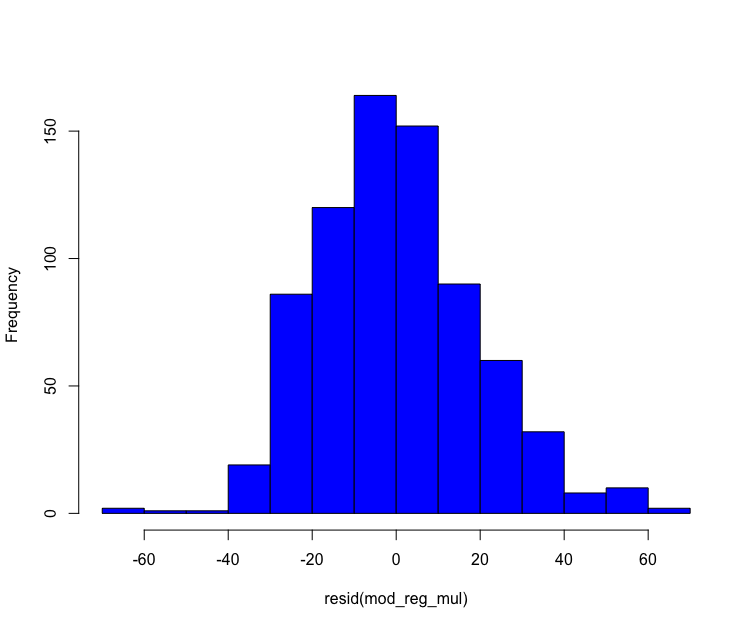
\includegraphics[scale=0.5]{ilu/cu.png}\end{center}\end{figure}

Nous obteenons donc un histogramme classique repr�sentant le termer r�siduel (le bruit) et l'on peut consid�rer graphiquement que les r�sidus du mod�le suivent bien une loi normale.\newline 
\\
En conclusion, dans ce chapitre, nous avons �tudi� : 
\begin{itemize}
\item La r�gression lin�aire multiple avec la fonction \textit{lm()} et la s�rie de variables explicatives correspondante.
\item La possibilit� d'ajouter une variable explicative cat�gorielle � plus de deux classes comme la variable profession et la n�cessit� de la recoder en une s�rie de variables binaires.
\item La possibilit� de changer la modalit� de r�f�rence de ces variables cat�gorielles � plus de deux classes, ce qui facilite l'interpr�tation des r�sultats.
\item La fonction \textit{drop1()} qui permet d'avoir l'effet global de cette variable cat�gorielle � plus de deux classes.
\item  La notion d'interaction entre deux variables explicatives quand le mod�le additif n?est potentiellement plus pertinent, avec le "multiplier" (x) que l'on met entre deux variables au lieu de les additionner.
\item La notion historique d'analyse de variance qui devrait �tre oubli�e au d�pend de la r�gression lin�aire multiple, avec n�anmoins la fameuse et classique analyse de variance � un facteur que l'on peut aussi r�aliser � l'aide de la fonction \textit{lm()}.
\item Les conditions de validit� de la r�gression lin�aire multiple, difficile � appr�cier, mais avec le minimum vital, l'appr�ciation de la normalit� des r�sidus � l'aide des fonctions \textit{hist()} et \textit{resid()}.
\end{itemize}
%%%%%%%%%%%%%%%%%%%%%%%%%%%%%%%%%%%%%%%%%%%%%%%%%%%%%%%%%%%%%%%
%%%%%%%%%%%%%%%%%%%%%%%%%%%%%%%%%%%%%%%%%%%%%%%%%%%%%%%%%%%%%%%
%%%%%%%%%%%%%%%%%%%%%%%%%%%%%%%%%%%%%%%%%%%%%%%%%%%%%%%%%%%%%%%
\chapter{Introduction � la r�gression logistique}
Apr�s la r�gression lin�aire, nous allons � pr�sent nous int�resser � la regression logisitique.\newline
\\
La r�gression logistique est classiquement utilis�e avec des variables binaires que l'on souhaite expliciter. Une telle situation peut �tre fr�quemment rencontr�e dans les sciences humaines et sociales ou encore en m�decine; Par exemple, si l'on souhaite expliquer les variables \textit{�tre au chomage} (oui,non), \textit{�tre s�par�} (oui,non) et \textit{avoir une maladie donn�e} (oui,non).\newline
Dans ce chapitre, nous allons nous int�resser � la question du \textit{risque suicidaire en prison} du fait du haut taux de ce dernier dans le mileu carc�ral. \newline
\\
Nous disposons d'une variable binaire : \textit{haut risque suicidaire} (cod�e en 0 et 1). Nous allons l'expliquer par une s�rie de variables explicatives possibles, parmi lesquelles par exemple, \textit{la dur�e de la peine}, \textit{l'existence de mesures disciplinaires}, \textit{l'existence d'ant�c�dents d'abus dans l'enfance}.\newline
Comme dans le chapitre sur la regression lin�aire multiple, nous avons ici une intrication possible des variables explicatives. En effet, il est possible d'imaginer que la dur�e de la peine est corr�l�e � l'existence de mesures disciplinaires. Si l'on suppose une peine longue, le d�tenu peut avoir tendance � s'�nerver et donc, recevoir des mesures disciplinaires. De la m�me fa�on, des abus dans l'enfance peuvent g�n�rer des troubles de la personnalit� qui peuvent �galement conduire � des comportements violent et donc, � des mesures disciplinaires, \dots (\textit{On peut en trouver plein des comme �a})\newline
Lorsque l'on va tenter de trouver des associations entres ces variables explicatives et la variable que l'on souhaite expliciter (� savoir le risque suicidaire), il serait particuli�rement utile de pouvoir d�m�ler le r�le et l'impact de chacune de ces variables explicatives.\newline
\\
Une premi�re approche consisterait � effectuer une regression lin�aire multiple entre expliquant la \textit{dur�e de l'incarc�ration}, l'\textit{existence d'un abus} et de \textit{mesures disciplinaires}.\newline

$$y= a + b\times\textrm{dur�e} + c\times\textrm{discip } + d\times\textrm{ abus} + bruit$$
avec $y$, le haut risque suicidaire.\newline
\\
le probl�me que l'on rencontre avec cette �quation, c'est que l'on conserve une variable r�siduelle � savoir le \textbf{bruit} qui poss�de une distribution \textbf{Normale}. Potentiellement, la droite $y$ (�quation ci dessus) varie entre $\pm \infty$ ce qui est incompatible dans le cadre de l'explicatiion d'une variable de type binaire ($0$ ou $1$).\newline 
\textcolor{red}{\textbf{De mani�re g�n�rale}}, la regression lin�aire multiple n'est applicable que dans les cas o� l'on souhaite expliquer des variables quantitatives puisque l'�quation de regression qui en r�sultera sera une combinaison lin�aire des variables explicatives et d'un terme de bruit.\newline
La r�gression lin�aire multiple n'est donc pas la m�thode la plus adequate pour expliquer des variables binaires.\newline 
\\
Les statisticiens ont trouv�s une astuce : \textit{Transformer la variable que l'on souhaite expliquer gr�ce � la fonction \textbf{logarithmique}}.\newline
\\
En reprenant le mod�le pr�c�dent et en repla�ant la valeur de $y$ : 
$$\log\left[\frac{P(\textrm{HRsuicide} = 1)}{1-P(\textrm{HRsuicide} = 1)}\right] = a + b\times\textrm{dur�e} + c\times\textrm{discip } + d\times\textrm{ abus}$$
\textit{Et pourquoi donc ? } car, par axiome, une probabilit� varie entre $[0,1]$ et donc, $\log\left[\frac{P(\textrm{HRsuicide} = 1)}{1-P(\textrm{HRsuicide} = 1)}\right]$ varie entre $]-\infty;+\infty[$ (C'est math�matique). La droite de r�gression lin�aire peut donc �tre obtenue par combinaison de variables explicatives que l'on souhaite.\newline
\\
\textbf{Note : } Puisque l'on r�gresse une probabilit� et non plus une variable, on suppose que le facteur \textit{bruit} du mod�le est nul.\newline
\\
L'�valuation des coefficient $a,b,d$ et $d$ seront calcul�s par \textbf{R}.\newline
\\
Dans l'exemple suivant, nous allons d�terminer l'influence de l'existence d'anth�cendents d'abus par r�gression logistique pour expliquer les hauts risques de suicide.\newline
\\
Nous allons tout d'abord commencer par un mod�le de r�gression logistique somple. Nous allons tenter d'expliquer la pr�sence d'un risque suicidaire (\textit{rs}) en fonction de la variable explicative : pr�sence d'ant�c�dents d'abus dans l'enfance.\newline 
S l'on se r�faire � la formule montr�e pr�c�demment, on peut �crire : 

$$\log\left[\frac{P(\textrm{rs} = 1)}{1-P(\textrm{rs} = 1)}\right] = a + b\times\textrm{ abus}$$

La fonction dans le logiciel \textbf{R} qui permet d'estimer une telle r�gression logisitique est la fonction \textit{glm()}, accronyme de \textit{Generalized Lineal Model}.\newline
La syntaxe de cette fonction est tr�s proche de celle que nous avons d�j� utilis� pour la fonction \textit{lm()}. 
\begin{center}
\textit{variable �tudi� $\sim$ variable explicative 1 + variable explicative 2 + \dots }
\end{center}
On doit de plus d�finir le type de variable explicative que l'on souhaite traiter. Dans notre cas, il s'agit d'une variable binomiale (succ�s/�checs, oui/non, 0/1, ...). Ainsi, nous ajoutons \textit{family="binomial"}.

\begin{lstlisting}[language=html]
> setwd("~/Desktop/DIVERS_TEMPLATES/R/TP")
> smp <-read.csv2("DONNEES/smp2.csv")
> mod <- glm(suicide.hr~abus, data = smp, family="binomial")
> summary(mod)

Call:
glm(formula = suicide.hr ~ abus, family = "binomial", data = smp)

Deviance Residuals: 
    Min       1Q   Median       3Q      Max  
-0.8446  -0.6020  -0.6020  -0.6020   1.8959  

Coefficients:
            Estimate Std. Error z value Pr(>|z|)    
(Intercept)  -1.6161     0.1154 -14.003  < 2e-16 ***
abus          0.7688     0.1897   4.052 5.07e-05 ***
---
Signif. codes:  0 ?***? 0.001 ?**? 0.01 ?*? 0.05 ?.? 0.1 ? ? 1

(Dispersion parameter for binomial family taken to be 1)

    Null deviance: 760.21  on 752  degrees of freedom
Residual deviance: 744.26  on 751  degrees of freedom
  (46 observations deleted due to missingness)
AIC: 748.26

Number of Fisher Scoring iterations: 4
\end{lstlisting}

On peut ainsi observer que pour cette r�gression, la valeur de $p$ est de $5.10^{-5}$; On peut donc en d�duire qu'avec un risque de $5\%$, il existe une association statistiquement signitificative entre les ant�c�dents d'abus dans l'enfance et un haut risque suicidaire pour un d�tenu incarc�r�.\newline
\\
Si l'on souhaite � pr�sent �tudier la valeur du coefficient $b$, nous devons �tudier la ligne \textit{Estimate} (Car pour le moment, c'est pas tr�s clair). Nous pouvons voir lire dans la console ci dessus que $b$ �quivaut � $0.7688$. \textit{Mais qu'est ce que cela signifie ?}\newline
Nous savons que $b$, correspondant � l'existence d'abus pendant l'enfance, est une variable binaire (cod�e sur $0$,$1$). On peut donc recourir � la fonction $t \longrightarrow e^{t}$ pour analyser le r�sultat ($e^{0} = 1$,$ e^{1}= 2,72$). On peut se rappeler que c'est l'\textbf{Odds Ratio}\footnote{L?odds ratio (OR) est une mesure statistique exprimant le degr� de d�pendance entre des variables al�atoires qualitatives - CF Chapitres pr�c�dents} qui associe des variables explicative avec des variables � expliquer.\newline
\\
\textbf{Note : } On rappelle que :
$$\log(\exp(a))=a$$
Cette propri�t� permet de r�tablir une valeur comprise entre $[-\infty,+\infty]$

\begin{lstlisting}[language=html]
> exp(0.7688)
[1] 2.157176
\end{lstlisting}

Si la variable � expliquer est suffisamment rare alors l'odds-ratio est voisin du risque relatif, ici, on a un odds-ratio de $2,15$, ce qui signifierait que des ant�c�dents d'abus dans l'enfance multiplient par $2$ la probabilit� d'�tre � haut risque suicidaire.\newline
\\
On obtient donc le mod�le suivant : 

$$\log\left[\frac{P(\textrm{rs} = 1)}{1-P(\textrm{rs} = 1)}\right] = a + 0,7688 \times\textrm{ abus}$$

On peut v�rifier la valeur de l'Odds Ratio en le calculant gr�ce � la fonction \textit{twoby2()} de la librairie $EPI$.

\begin{lstlisting}[language=html]
> library(Epi)
> twoby2(1-smp$suicide.hr, 1-smp$abus)
2 by 2 table analysis: 
------------------------------------------------------ 
Outcome   : 0 
Comparing : 0 vs. 1 

    0   1    P(0) 95\% conf. interval
0  63  90  0.4118    0.3366   0.4913
1 147 453  0.2450    0.2122   0.2810

                                   95\% conf. interval
             Relative Risk: 1.6807    1.3276   2.1276
         Sample Odds Ratio: 2.1571    1.4873   3.1287
Conditional MLE Odds Ratio: 2.1547    1.4577   3.1764
    Probability difference: 0.1668    0.0837   0.2525

             Exact P-value: 1e-04 
        Asymptotic P-value: 1e-04 
------------------------------------------------------
> exp(0.7688)
[1] 2.157176
\end{lstlisting}
Nous obtenons effectivement une valeur du Odds Ratio �gale � $e^{0.7688} = 2.157176$.
%%%%%%%%%%%%%%%%%%%%%%%%%%%%%%%%%%%%%%%%%%%%%%%%%%%%%%%%%%%%%%%
%%%%%%%%%%%%%%%%%%%%%%%%%%%%%%%%%%%%%%%%%%%%%%%%%%%%%%%%%%%%%%%
%%%%%%%%%%%%%%%%%%%%%%%%%%%%%%%%%%%%%%%%%%%%%%%%%%%%%%%%%%%%%%%
\chapter{R�gression logistique avec plusieurs variables explicatives}
Nous allons maintenant nous int�resser aux r�gressions logistiques pour des mod�les comportant plusieurs variables explicatives.\newline
\\
Dans ce chapitre, nous allons nous poser la question suivante : \textit{Est-ce qu'un haut risque suicidaire en prison est associ� � : 
\begin{enumerate}
\item � la dur�e d'incarc�ration
\item � des mesures disciplinaires
\item � des ant�c�dents d'abus dans l'enfance
\end{enumerate}}
Pour ce faire, nous allons utiliser une r�gression logistique que l'on peut qualifier de multiple comme une regression lin�aire multiple. Voici le mod�le que nous allons �tudier : 
$$\log\left[\frac{P(\textrm{HRsuicide} = 1)}{1-P(\textrm{HRsuicide} = 1)}\right] = a + b\times\textrm{dur�e} + c\times\textrm{discip } + d\times\textrm{ abus}$$
La fonction correspondante est la fonction \textit{glm()} avec la syntaxe suivante : 
\begin{itemize}
\item La variable � expliquer
\item Un tilde $\sim$
\item Les variables explicatives
\item Le nom du dataframe dans lequel nous trouvons les variables 
\item l'instruction \textit{family="binomial"} pour sp�cifier que nous allons r�aliser une r�gression logistique
\end{itemize}
La ligne de commande est donc : 
\begin{lstlisting}[language=html]
smp <- read.csv2("smp2.csv")
mod_reg_log = glm(suicide.hr~abus+discip+duree,data= smp, family = "binomial")
\end{lstlisting}
Nous allons donc stocker le tout dans un objet et utiliser la fonction \textit{summary()}.\newline

\begin{lstlisting}[language=html]
> mod_reg_log = glm(suicide.hr~abus+discip+duree,data= smp, family = "binomial")
> summary(mod_reg_log)

Call:
glm(formula = suicide.hr ~ abus + discip + duree, family = "binomial", 
    data = smp)

Deviance Residuals: 
    Min       1Q   Median       3Q      Max  
-1.3200  -0.6655  -0.6012  -0.4997   2.0700  

Coefficients:
            Estimate Std. Error z value Pr(>|z|)    
(Intercept) -0.02462    0.49635  -0.050 0.960439    
abus         0.62289    0.22764   2.736 0.006213 ** 
discip       0.52809    0.23767   2.222 0.026287 *  
duree       -0.39862    0.11723  -3.400 0.000673 ***
---
Signif. codes:  0 ?***? 0.001 ?**? 0.01 ?*? 0.05 ?.? 0.1 ? ? 1

(Dispersion parameter for binomial family taken to be 1)

    Null deviance: 555.94  on 549  degrees of freedom
Residual deviance: 533.26  on 546  degrees of freedom
  (249 observations deleted due to missingness)
AIC: 541.26

Number of Fisher Scoring iterations: 4
\end{lstlisting}

on obtient ainsi les r�sultats suivant : 


\begin{center}
\begin{tabular}{c|c|c|}
\hline
 & \textbf{Estimate} & \textbf{Pr$(>|z|)$} \\ \hline
\multicolumn{1}{|c|}{\textbf{abus}}   & 0.62289           & 0.006213            \\ \hline
\multicolumn{1}{|c|}{\textbf{discip}} & 0.52809           & 0.026287            \\ \hline
\multicolumn{1}{|c|}{\textbf{duree}}  & -0.39862          & 0.000673            \\ \hline
\end{tabular}
\end{center}

Nous pouvons, dans un premier temps, regarder les valeurs de $p$ ($Pr(>|z|)$) et on remarque que ces derni�res sont toutes inf�rieures � $5\%$. On peut donc en d�duire que ces trois variables explicatives sont statistiquement associ�es � un haut risque suicidaire, et ce, toutes choses �gales et par ailleurs (\textit{ceteris paribus}), en tout cas "toutes choses", tous param�tres mesur�es et inclus dans le mod�le, plus pr�cisement.\newline
\begin{itemize}
\item Des ant�c�dents d'abus dans l'enfance sont statistiquement associ�s � un haut risque suicidaire, et cen � mesures disciplinaires �ventuelles constantes et � dur�e d'incarc�ration constante.
\item La dur�e d'incarc�ration est statistiquement associ�e au risque suicidaire et ce, m�me compte tenu d'�ventuelles mesures disciplinaires et d'un �ventuel ant�c�dent d'abus dans l'enfance.
\end{itemize}

Le mod�le obtenu est donc le suivant : 

$$\log\left[\frac{P(\textrm{HRsuicide} = 1)}{1-P(\textrm{HRsuicide} = 1)}\right] =  -0.02+ 0.63\times\textrm{dur�e} + 0.53\times\textrm{discip } -0.40 \times\textrm{ abus}$$

Si nous nous int�ressons plus en d�tail aux coefficients de la colonne \textit{Estimate} et que nous �tudions leurs signes, nous pouvons interpr�ter ce signe en fonction du codage des variables explicatives. \newline
Dans notre cas, le codage est le suivant : 
\begin{itemize}
\item $1$ pour abus, $0$ pour pas d'abus
\item $1$ pour mesures disciplinaires , $0$ pour absence de mesures disciplinaires
\item la variable dur�e, elle, est cod�e de 1 � 5 ; plus la variable est �lev�e, plus la dur�e d'incarc�ration est longue.
\end{itemize}
Autrement dit, ces trois variables sont cod�es de la mani�re suivante : plus elles sont �lev�es, plus le niveau d'exposition, le niveau du risque est �lev�. \newline 
Th�oriquement, si ces trois variables sont des facteurs de risque, nous devrions avoir une augmentation du risque correspondant et donc des coefficients positifs.\newline
On peut observer que c'est bien le cas pour les variables explicatives repr�sentant l'abus et les mesures disciplinaires mais, que c'est le contraire pour la variables correspondant � la dur�e.\newline
Dans les faits et contrairement � ce que l'on aurait pu penser, une dur�e d'incarc�ration �lev�e diminue la probabilit� d'�tre � haut risque suicidaire. 
Nous venons donc de r�aliser l'analyse du signe des coefficients du mod�le de r�gression logistique; �tape \textcolor{red}{tr�s importante}.\newline
\\
Nous pouvons maintenant tenter d'interpr�ter l'amplitude des coefficients et n'oubliant pas que sous cette forme, ces derniers ne sont pas interpr�tables (Nous sommes dans une expression logarithmique). Nous devons donc appliquer l'instruction \textit{exp()} sur les coefficients, r�cup�r�s gr�ce � la fonction \textit{coefficients()}.
\begin{lstlisting}[language=html]
> exp(coefficients(mod_reg_log))
(Intercept)        abus      discip       duree 
  0.9756803   1.8643147   1.6956873   0.6712485 
\end{lstlisting}
Nous obtenons ainsi des r�sultats autour de $1,9$ et $1,7$. Nous pouvons ainsi en d�duire que l'existence d'ant�c�dents d'abus dans l'enfance multiplie quasiment par $2$ le risque de pr�senter de haut risque suicidaire en prison et ceci, ind�pendamment de l'existence de mesures disciplinaireset de la dur�e d'incarc�ration.\newline
Concernant la dur�e d'incarc�ration, cette derni�re n'est pas binaire (cod�e sur 0 et 1). La question qui se pose alors est de savoir comment interpr�ter le coefficients $0,7$. Il s'agit en fait du coefficient multiplicateur entre deux changement de modalit� dans la variable dur�e. \newline
Si l'on consid�re le codage de la variable dur�e suivant : la dur�e d'incarc�ration d�finie par $1$ correspond � moins de 1 mois de d�tention; par 2, de 1 � 6 mois; par 3 : de 6 mois � 1 an; par 4, de 1 � 5 ans et par 5, plus de 5 ans.\newline
Lorsque l'on passe d'une modalit� vers une modalit� sup�rieure, le niveau de haut risque suicide diminue d'environ $(1-0,7) = 0,3$ soit $30\%$ ($0,3$ �tant le compl�ment de l'Odds-Ratio que l'on a ici, voisin de $0,7$).\newline
\\
Dans le cadre d'une r�gression logistique � plusieurs variables, on peut retrouver certaines similitudes avec une r�gression lin�aire multiple : Par exemple, il est possible d'ins�rer dans le mod�le, des variables cat�goricielles � plus de deux classes; \textbf{R} recodera automatiquement ces derni�res en $k-1$ variables binaires (en supposant que l'on a initialement $k$ modalit�s dans la variable cat�goricielle). Nous aurons ainsi $k-1$ valeurs de $p$ et des coefficnets qui seront � interpr�ter par rapport � une modalit� de r�f�rence (que l'on pourra �galement changer).\newline
De plus, si nous souhaitons analyser l'effet global de la variable cat�goricielle sur la variable que l'on souhaite �tudier, nous utiliserons �galement la fonction \textit{drop1()} avec la m�me syntaxe sauf que cette fois ci, nous �crirons \textit{\textcolor{red}{test="Chisq"}} � la place de \textit{test="F"}.\newline
De la m�me mani�re, il est aussi possible d'essayer de trouver des synergies entre des variables explicatives, c'est � dire mettre des termes en interaction. Par exemple, nous avons vu pr�c�demment que la dur�e d'incarc�ration et les mesures disciplinaires �taient des facteurs de risque suicidaire. Nous pouvons imaginer qu'un d�tention, au d�but de sa peine c'est � dire, au moment ou les risque suicidaire est important, se voit imposer une mesure disciplinaire. On peut imaginer que les deux facteurs de risque g�n�rent un risque qui peut �tre beaucoup plus important que la sommation simple des deux risques. Il y aurait donc une synergie entre les facteurs de risque. Il fautdrait alors introduire un terme d'interaction, qui serait quant � lui, caract�ris� par le produit des deux variables et nous interpr�terions les r�sultats de la m�me mani�re que dans le chapitre sur les r�gressions lin�aires multiples.\newline
\\
Int�ressons nous maintenant aux conditions de validit� d'une r�gression logistique. Ces derni�res sont encore plus compliqu�es que celles pour une r�gression lin�aire.\newline
Pour simplifier l'ensemble des conditions de validit� et aller � l'essentiel, on pourra se souvenir qu'il faut au minimum entre $5$ et $10$ �v�nements par variable explicative.\newline
Dans le dataframe \textit{sant� mentale en prison}, nous avons $799$ d�tenus.

\begin{lstlisting}[language=html]
> table(smp$scz.cons)

  0   1 
733  66 
\end{lstlisting}
Si l'on s'int�resse � la variable explicative \textit{schizophr�nie consensuelle (scz.cons)} caract�risant les d�tenus avec une forme grave de schizophr�nie, nous en avons alors 66.\newline
D�s lors, imaginons que nous cherchions � expliquer ces troubles de la personnalit� en fonction de l'�ge, d'existence d'un trauma durant l'enfance et de la profession. Nous r�aliserions alors un mod�le de r�gression logistique � trois variables.\newline
les variables \textit{age} et \textit{abus} sont des variables binaires non recod�es. Pour la variable \textit{profession}, c'est une variable explicative comportant 8 modalit�s, recod�e en 7 variables binaires. Le mod�le comporte donc $1+1+7 = 9$ variables binaires explicatives.\newline
Pour que la mod�le de r�gression logistique soit valide, il faut entre $5$ et $10$ �v�nements par variable explicative.\newline
Prenons la contrainte la plus forte, � savoir $10$ �v�nements par variable explicative. Il faudrait donc $(1+1+7)\times 10 = 90$ d�tenus au minimum pour que la r�gression logistique soit valide; Or, nous n'en avons que $66$. Par cette premi�re contrainte, on peut en d�duire que ce mod�le de r�gression logistique n'est pas pertinent.\newline
Prenons la contrainte la plus forte, � savoir $10$ �v�nements par variable explicative. Il faudrait donc $(1+1+7)\times 5 = 45$ d�tenus au minimum pour que la r�gression logistique soit valide; Or, nous avons $66$. Par cette seconde contrainte, on peut en d�duire que ce mod�le de r�gression logistique est pertinent.\newline
En conclusion, sous la contrainte n�$1$, il nous faudrait au minimum $90$ d�tenus atteints de schizophr�nie pour expliquer ce trouble par les variables \textit{age},\textit{abus} et \textit{profession} et sous la contrainte n�$2$, il nous faut au minimum $45$ d�tenus atteints de schizophr�nie pour expliquer ce trouble par ces m�mes variables.


%%%%%%%%%%%%%%%%%%%%%%%%%%%%%%%%%%%%%%%%%%%%%%%%%%%%%%%%%%%%%%%
%%%%%%%%%%%%%%%%%%%%%%%%%%%%%%%%%%%%%%%%%%%%%%%%%%%%%%%%%%%%%%%
%%%%%%%%%%%%%%%%%%%%%%%%%%%%%%%%%%%%%%%%%%%%%%%%%%%%%%%%%%%%%%%
\chapter{Donn�es censur�es, survie : vocabulaire et approches descriptives}
Nous allons maintenant �tudier des donn�es censur�es parmi lesquelles, la survie\footnote{L'analyse de (la) survie est une branche des statistiques qui cherche � mod�liser le temps restant avant la mort pour des organismes biologiques (l'esp�rance de vie) ou le temps restant avant l'�chec ou la panne dans les syst�mes artificiels, ce que l'on repr�sente graphiquement sous la forme d'une courbe de survie. } est un exemple classique.\newline
Nous allons tout d'abord nous focaliser sur le vocabulaire utilis� dans ce domaine et sur les approches statistiques descriptives qui lui sont propres.\newline
\\
Il n'est pas rare que des mesures effectu�es dans des �tudes correspondent � des dur�es. Ce sera par exemple le cas si l'on analyse un groupe de sujets au ch�mage que l'on aura suivi pendant un an. Durant cette p�riode, nous aurons mesur� le temps jusqu'� recouvrement du travail.\newline
Cela pourra �tre �galement le cas si nous prenions en charge un groupe de patients ayant un infarctus du myocarde et que nous les suivions jusqu'� l'obtention d'une r�cidive ou du d�c�s.\newline
Ces dur�es ont comme particularit� qu'elles peuvent �tre potentiellement censur�es.\newline
Qu'est ce qu'une \textit{statistique censur�e} ? Dans le cas o� nous avons la charge d'un groupe de sujets que nous avons suivi pendant un an, certains sujets vont avoir retrouv� du travail au bout de 2 mois, 4 mois, 6 mois \dots Pour ces sujets, on connait exactement la dur�e jusqu'au recouvrement de travail. Cependant pour d'autres membres du groupe, au bout d'un an, certains n'auront pas retrouv� de travail. Donc, le temps jusqu'� recouvrement du travail de certains individus ne sera pas connu par manque de suivi. Mais, on saura tout de m�me que le temps de recouvrement est sup�rieur � un an. Dans ce cas l�, lorsque l'on a qu'une \textbf{connaissance partielle de la variable mesur�e}, on dit qu'une \textbf{variable est censur�e}.\newline 
\\
Les statisticiens ont d�velopp� de nombreuse m�thodes sp�cifiquement adapt�es � l'analyse des donn�es censur�es, ce que nous allons �tudier dans ce chapitre.\newline 
\\
Nous pourrions nous dire que le changement de variable � �tudier serait une bonne mani�re de ne pas avoir � �tudier des donn�es censur�es. Par exemple, plut�t que d'�tudier la variable \textit{dur�e jusqu'� survenue de l'�v�nement}, nous pourrions �tudier la variable \textit{pourcentage de survenue de l'�v�nement}. On pourrait �galement �tudier \textit{pourcentage de ch�meur ayant retrouv� du travail en un an} plut�t que d'�tudier \textit{dur�e jusqu'� recouvrement de travail}.\newline
Cependant, lorsque nous r�alisons une �tude, nous ne sommes jamais s�r de pouvoir suivre les sujets pendant la totalit� de la p�riode (par exemple, �tude d'un groupe de personnes au ch�mage sur an). En effet, il est possible que l'inclusion (d'un individu dans le groupe) puisse durer longtemps et que nous n'avons pas le temps d'attendre un an une fois que les derniers sujets ont �t� inclus. il est �galement possible que certains sujets d�m�nagent et, � ce moment l�, soient perdus de vue.\newline
Si nous �tudions le pourcentage de survenue de l'�v�nement � un an, tous ces sujets, nous serons oblig�s de les abandonner et cela peut induire des biais ou une perte de puissance.\newline
\\
Dans le domaine des donn�es de survie, il existe un vocabulaire tr�s sp�cifique que l'on doit connaitre.\newline
Le permier �l�ment de langage est la notion m�me de \textbf{survie}. Largement abusive car en g�n�ral, on ne s'int�resse pas aux d�c�s des individus mais au d�lai jusqu'� survenue d'un �v�nement. Mais comme le d�lai de survie est effectivement le d�lai jusqu'a survenue d'un �v�nement (et l�, nous parlons de la mort de cet individu), alors de fa�on m�taphorique, nous parlons de donn�es de survie bien qu'il s'agisse que d'un d�lai jusqu'� survenue d'un �v�nement et que ce dernier n'est en g�n�ral pas la mort de cet individu.\newline
Le deuxi�me point est la notion de \textbf{censure}. Nous avons bri�vement vu ce que ce terme signifiait mais sur un plan m�thodologique, il est important de diff�rencier deux types de censures : 
\begin{itemize}
\item Le premier correspond aux \textit{exclus vivants}. Nous devrions suivre les patients pendant une p�riode (un an), nous les suivons sur toute cette p�riode (un an) et � la fin de cette p�riode (d'un an), certains individus sont vivants. On parle d'exclus vivants. 
\item Le second correspond aux \textit{perdus de vue}. Nous devrions suivre les patients pendant une p�riode et puis, au bout de trois mois, le patient d�m�nage. On dit alors que le patient est perdu de vue mais il n'a pas �t� suivi pendant un an. 
\end{itemize}

Ces deux types de censures sont diff�rentes car il est tout � fait possible que des patients, perdus de vue, aient des biais\footnote{En statistique ou en �pid�miologie, un biais est une d�marche ou un proc�d� qui engendre des erreurs syst�matiques dans les r�sultats d'une �tude.} qui soient diff�rents que des exclus vivants. En effet, le fait qu'un patient d�m�nage peut �tre possiblement li� au fait qu'il se trouve en bonne sant� ou au contraire, en mauvaise sant�, ce qui sera diff�rent des exclus vivants. De l�, la n�cessit� de bien diff�rentier les deux types de censure.\newline
\\
Dans le cadre de l'analyse des donn�es de survies, il faut �galement d�finir l'�l�ment statistique suivant : \textit{la fonction de survie}\newline
Le terme de survie est �galement utilis� de mani�re abusive. En effet, la fonction de survie repr�sente le pourcentage des sujets survivants au cours du temps ou, le pourcentage de sujets qui n'ont pas encore obtenu l'�v�nement au cours du temps. C'est une fonction n�c�ssairement d�croissante qui part de $100\%$ (la totalit� du groupe) � $0\%$ (si tous les membres du groupe d�c�de un jour).\newline
Enfin, il faut �galement d�finir la notion de \textit{risque instantant� de d�c�s} qui est une notion plus abstraite (car plus math�matique).\newline
Avec ce type de donn�es, il serait int�ressant de pouvoir d�crire au cours du temps, l'�volution de la probabilit� de d�c�der et ceci, � un instant donn�. Cependant, la probabilit� de d�c�der � un instant donn� est $0$ (consid�r�e comme l'�v�nement impossible); la probabilit� de mourir un jour donn� est un nombre \textit{petit} alors que la probabilit� de mourir � une minute donn�e est un nombre \textit{quasiment microscopique} qui n'a pas de sens.?newline
On ne peut donc pas repr�senter la fonction de risque instantant� de d�c�s.\newline
Cependant, les math�maticiens ont d�velopp� gr�ce aux fonctions d�riv�es, une fonction que l'on appelle $h(t)$ qui permet d'obtenir une approximation d'une probabilit� ponctuelle. $h(t)$ est alors appell� \textit{risque instantan� de d�c�s}.\newline
\\
Nous allons � pr�sent voir comment repr�senter graphiquement la fonction de survie. Pour ce faire, nous allons prendre pour exemple un essai qui a �tudi� le premier m�dicament v�ritablement efficace dans le cadre du traitement de la leuc�mie.

\begin{figure}[H]\begin{center}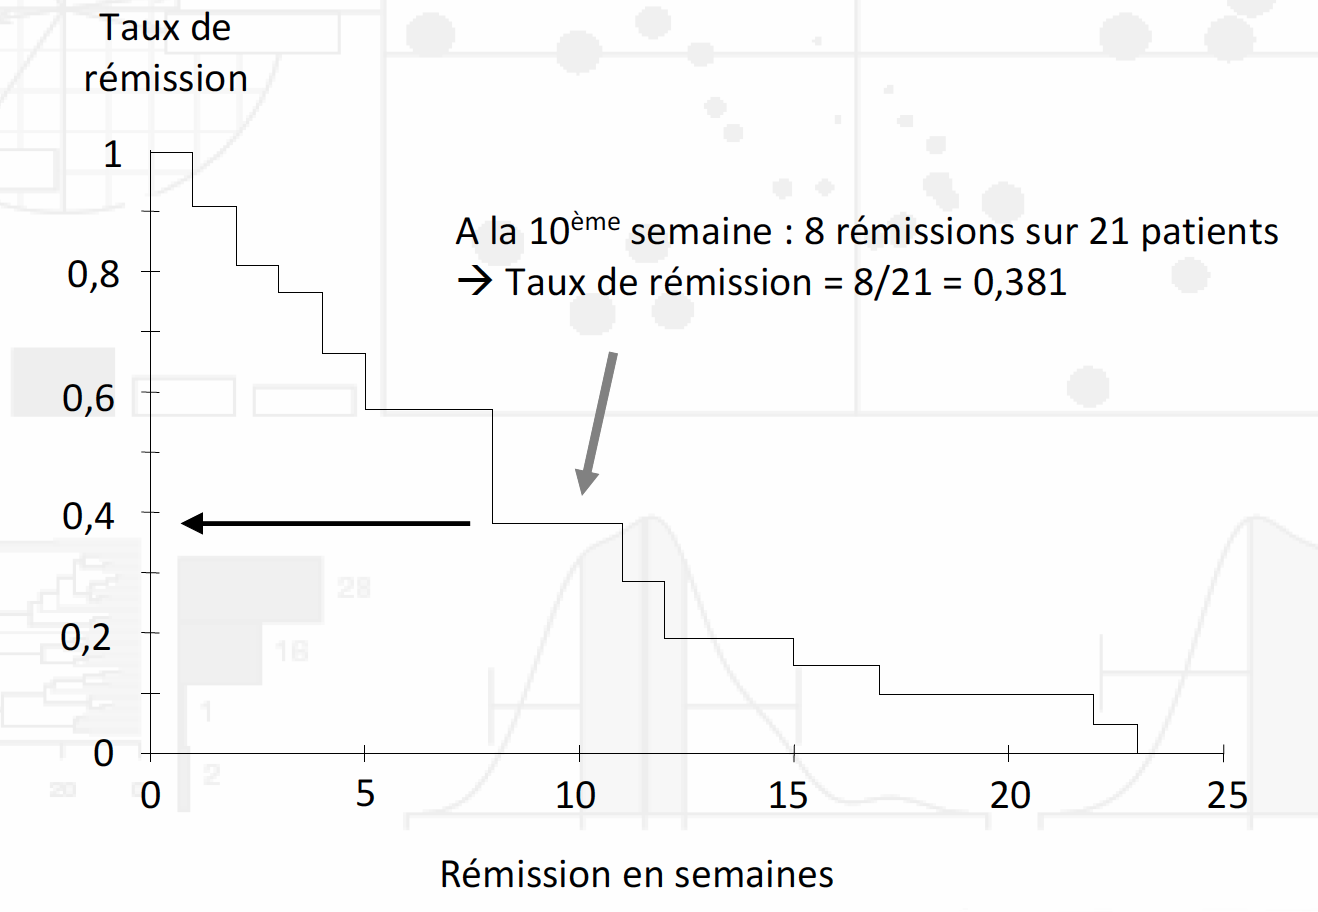
\includegraphics[scale=0.5]{ilu/dsurv1.png}\end{center}\end{figure}

Sur ce graphique, nous pouvons analyser le taux de r�mission exprim� en semaine alors que l'on utilisait encore un traitement � base de cortico�des. Ce dernier op�rait quelques semaines mais il y avait tr�s vite un �chappement th�rapeutique\footnote{l'�chappement th�rapeutique est le fait, pour un traitement, de devenir inefficace apr�s une p�riode d'efficacit�.} au bout de $15$ � $20$ semaines et l'ensemble des patients mourraient.\newline
Dans ce cas, la fonction de survie est facilement repr�sentable : Comme nous avons suivi les sujets jusqu'� leurs d�c�s, nous pouvons calculer au fil du temps, le pourcentage de sujets survivants et l'on obtient le graphique ci-dessus.

\begin{figure}[H]\begin{center}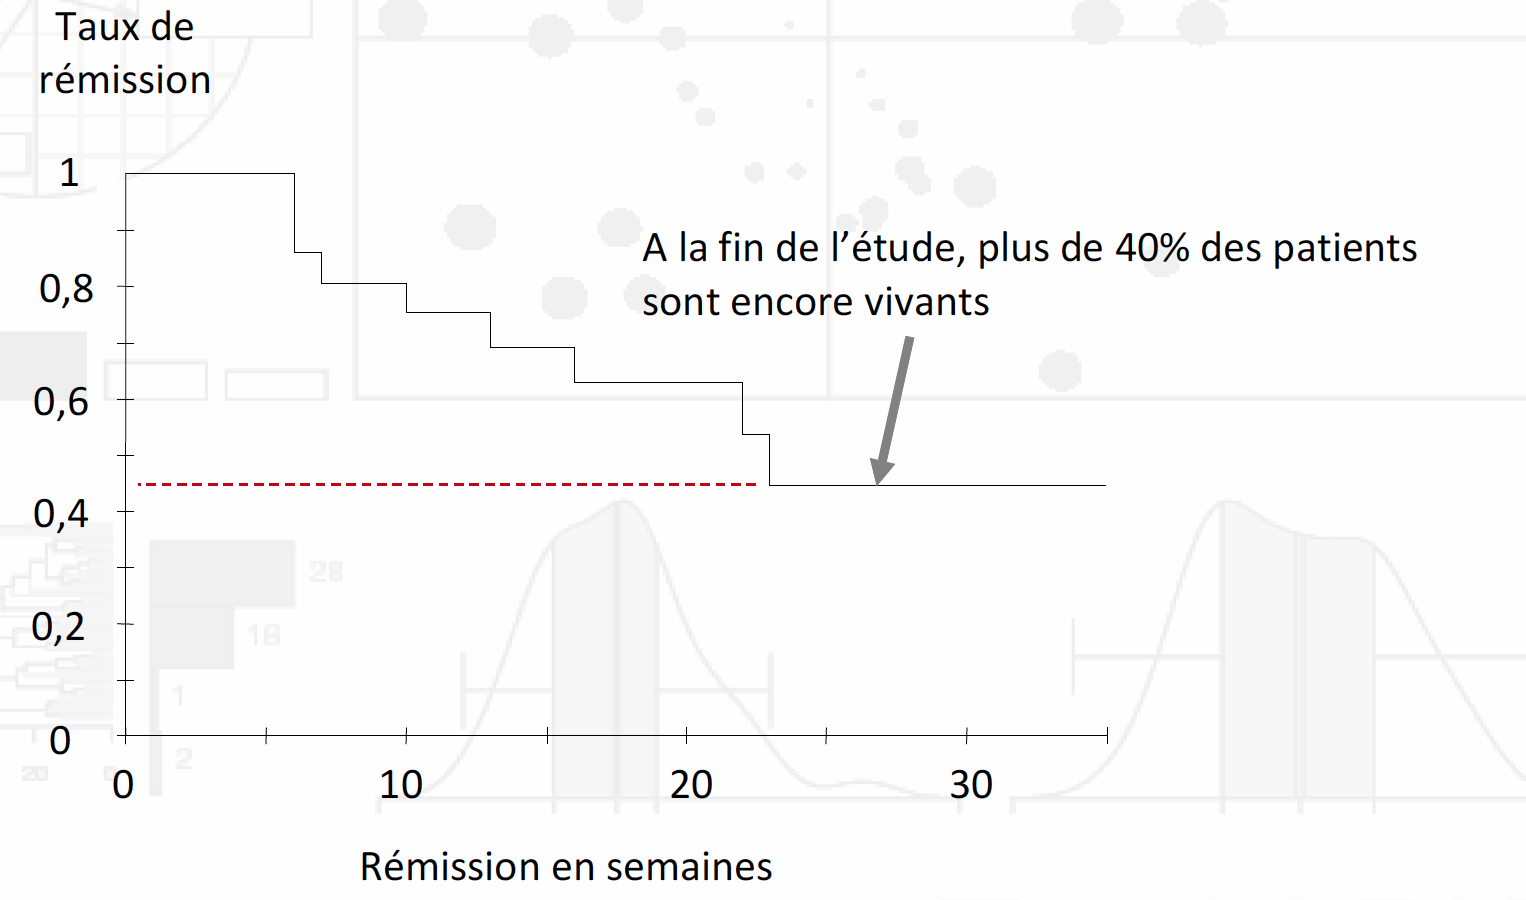
\includegraphics[scale=0.5]{ilu/dsurv2.png}\end{center}\end{figure}
Dans le cadre du second traitement, � la fin de l'essau et du suivi des patients, on peut observer que $40\%$ des sujets sont encore en vie. Il se pose  alors la question de la repr�sentation de la fonction de survie.\newline
En effet, au fur et � mesure que le temps passe, le num�rateur change car il correspond au nombre de sujets survivant mais de plus, le d�nominateur change �galement car il repr�sente le nombre de sujets encore vivants qui continuent a �tre observ�s. Cela devient donc d�licat de calculer de mani�re non biais�e, avec un tel jeu de donn�es, le pourcentage de survivants c'est � dire, la fonction de survie.\newline
Les statisticiens ont alors d�velopp� une m�thode connue sous le nom de \textit{M�thode de Kaplan - Meier}.\newline
\\
Pour �tudier la m�thode de Kaplan - Meier � l'aide du logiciel \textbf{R}, nous allons nous int�resser � un nouveau dataset\footnote{l'�tude sant� mentale en
prison �tant une �tude transversale, nous n'avons pas de suivi de patients. Nous n'avons donc pas de dur�e jusqu'� survenue d'un �v�nement et donc pas de donn�es censur�es.}, cette fois ci compos� de $125$ patients alcooliques qui ont �t� hospitalis�s puis sevr�s. Ces patients ont �t�s suivis et nous avons � notre disposition les $5$ variables suivantes : 
\begin{enumerate}
\item Le d�lai d'observation t
\item Le fait que les patients soient toujours sevr�s � la fin de l'�tude 
\begin{itemize}
\item $1$ : ils ont rechut�s
\item $0$ : ils sont toujours sevr�s
\end{itemize}
\item l'�ge
\item Le sexe du patient 
\item L'existence d'un �v�nement de vie n�gative pendant le suivi 
\begin{itemize}
\item $1$ : Oui 
\item $0$ : Non 
\end{itemize}
\end{enumerate}

\begin{lstlisting}[language=html]
> alc <- read.csv2("DONNEES/alcool.csv")
> str(alc)
'data.frame': 125 obs. of  5 variables:
 $ t     : int  121 121 40 39 66 64 5 30 34 5 ...
 $ SEVRE : int  0 0 0 0 0 0 1 0 0 0 ...
 $ AGE   : int  53 52 45 48 45 42 35 35 41 37 ...
 $ SEXE  : int  1 2 2 1 1 1 1 1 1 1 ...
 $ EDVNEG: int  0 0 0 1 0 0 0 0 0 0 ...
\end{lstlisting}

Gr�ce � ce nouveau jeu de donn�es, la variable censur�e que nous allons �tudier correspond au d�lai jusqu'� la survenue de l'�v�nement : \textit{"Rechute de la maladie alcoolique"}.\newline
\\
Pour tracer la fonction de survie de cette variable censur�e, nous allons utiliser la librairie \textit{survival} qui contient l'ensemble des m�thodes adapt�es aux donn�es censur�es.\newline
\\
Nous allons utiliser trois fonction successivement : la fonction \textit{plot()}, la fonction \textit{survfit()}\footnote{This function creates survival curves from either a formula (e.g. the Kaplan-Meier), a previously fitted Cox model, or a previously fitted accelerated failure time model.} et la fonction \textit{Surv()}\footnote{Create a survival object, usually used as a response variable in a model formula. }. La syntaxe de est alors la suivante : 
\begin{itemize}
\item On met tout d'abord le d�lai de survi \textit{t}
\item Puis la variable survenue de l'�v�nement \textit{SERVE} (perte du sevrage)
\item puis $\sim 1$
\end{itemize}



\begin{lstlisting}[language=html]
library(survival)
plot(survfit(Surv(alc$t,alc$SEVRE)~1),main="Courbe de maintien de l'abstinence",xlab="Temps",ylab = "%")
\end{lstlisting}
Nous obtenons alors en trait plein, la fonction de survie et en trait pointill�, l'intervalle de confiance � $95\%$ de la fonction de survie. 

\begin{figure}[H]\begin{center}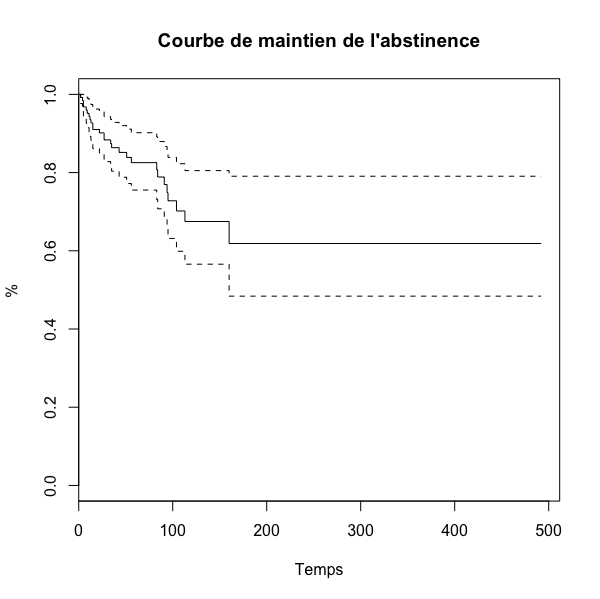
\includegraphics[scale=0.5]{ilu/dsurv3.png}\end{center}\end{figure}

En modifiant la syntaxe, on peut repr�senter graphiquement et sur un m�me sch�ma, plusieurs courbes de survie correspondant � la survie de diffrents groupes de sujets. Par exemple, si nous souhaitons repr�senter sur un m�me graphique, le temps jusqu'� la rechute de la maladie alcoolique chez les hommes et chez les femmes, il suffit alors de remplacer $\sim 1$ par $\sim SEXE$. Nous ajoutons �galement des couleurs afin de mettre avant le sexe du sujet : 

\begin{lstlisting}[language=html]
plot(survfit(Surv(alc$t,alc$SEVRE)~alc$SEXE),col=c("blue","red"),main="Courbe de maintien de l'abstinence",xlab="Temps",ylab = "%")
## Variante possible pour simplifier l'�criture : survfit(Surv(t,SEVRE)~SEXE,data=alc)
\end{lstlisting}

\begin{figure}[H]\begin{center}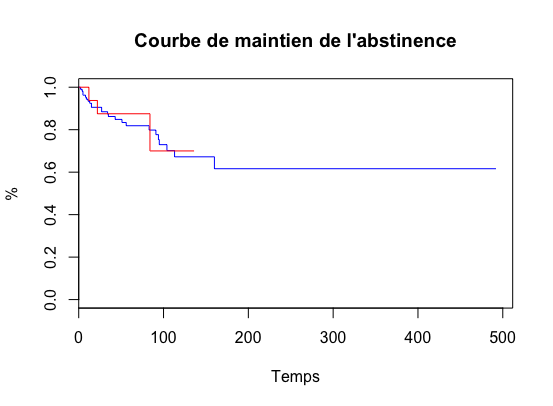
\includegraphics[scale=0.5]{ilu/dsurv4.png}\end{center}\end{figure}

Il existe des statistiques agr�g�es qui sont plus sp�cifiques � l'�tude des donn�es censur�es. On peut par exemple �voquer la \textit{m�diane de survie} qui correspond au moment o� $50\%$ des sujets n'ont pas encore subit la survenue de l'�v�nement et $50\%$ des sujets l'ont subit.\newline
Pour obtenir ces donn�es, il suffit juste de r�utiliser la syntaxe que nous venons d'�crire en enlevant la fonction \textit{plot()} : 
\begin{itemize}
\item On met tout d'abord le d�lai de survi \textit{t}
\item Puis la variable survenue de l'�v�nement \textit{SERVE} (perte du sevrage)
\item puis $\sim 1$
\end{itemize}

\begin{lstlisting}[language=html]
survfit(Surv(t,SEVRE)~SEXE,data=alc)
Call: survfit(formula = Surv(t, SEVRE) ~ SEXE, data = alc)

         n events median 0.95LCL 0.95UCL
SEXE=1 107     24     NA     160      NA
SEXE=2  18      3     NA      84      NA
\end{lstlisting}
Dans notre cas, la m�diane de survie n'est pas obtenue (on peut observer un NA qui correspond � une donn�e manquante); Cela signifie tout simplement qu'� la fin de l'�tude c'est � dire � la fin du delai de suivi, plus de $50\%$ des patients sont toujours sevr�s et qu'il nous est donc impossible d'estimer une m�diane de survie.

%%%%%%%%%%%%%%%%%%%%%%%%%%%%%%%%%%%%%%%%%%%%%%%%%%%%%%%%%%%%%%%
%%%%%%%%%%%%%%%%%%%%%%%%%%%%%%%%%%%%%%%%%%%%%%%%%%%%%%%%%%%%%%%
%%%%%%%%%%%%%%%%%%%%%%%%%%%%%%%%%%%%%%%%%%%%%%%%%%%%%%%%%%%%%%%
\chapter{Donn�es censur�es, survie : tests statistiques et mod�lisation}
Nous allons � pr�sent nous int�resser aux tests statistiques et aux mod�les multivari�s que l'on peut r�aliser sur des donn�es censur�es.\newline
\\
Dans le chapitre pr�c�dent, nous avons repr�sent� sur un m�me graphique, les fonctions de survie relatives � la rechute de la maladie alcoolique chez un groupe de femmes et chez un groupe d'homme. 

\begin{figure}[H]\begin{center}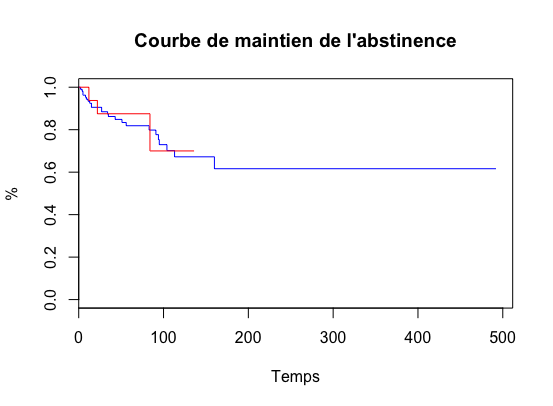
\includegraphics[scale=0.5]{ilu/dsurv4.png}\end{center}\end{figure}

On peut observer que les deux courbes ont l'air de se superposer. Mais on peut �galement se poser la question et tester statistiques si il existe une diff�rence des taux de rechute entre les hommes et les femmes. Pour r�aliser ce test, nous devons utiliser la m�thode du \textit{Log-Rank}.\newline
\\
Le test du \textit{Log-Rank} est assimil� � un test de rangs; les rangs entre les temps de d�c�s comme nous avons pu le voir dans le test de \textit{Wilcoxon}.\newline
Les conditions de validit� de la m�thode du Log-Rank sont plus d�licates.\newline
La principale conditions de validit� est la quantit� de temps de d�c�s. Si \underline{il y a de nombreux temps de d�c�s, alors le test du Log-Rank est valide}.\newline
Dans le cadre de notre �chantillon, si nous suivons des sujets et que nous effectuons des observations seulement tous les six mois, alors nous aurons peu de temps de d�c�s mais il y aura beaucoup de d�c�s sur chaque observations. Cette seconde configuration permet �galement d'assurer la validit� du test du Log-Rank. Quand \underline{il y a de nombreux morts � chaque temps de d�c�s, le test est �galement valide}.\newline
\\
Nous allons donc effectuer le test du Log-Rank sur notre jeu de donn�e. La syntaxe est la suivante, nous allons utiliser la fonction \textit{survdiff()}\footnote{Tests if there is a difference between two or more survival curves using the G-rho family of tests, or for a single curve against a known alternative.} de la mani�re suivante :\textit{survdiff(Surv(d�lai,�v�nement)$\sim$classe)}

\begin{lstlisting}[language=html]
alc <- read.csv2("DONNEES/alcool.csv")
> survdiff(Surv(t,SEVRE)~SEXE,data=alc)
Call:
survdiff(formula = Surv(t, SEVRE) ~ SEXE, data = alc)

         N Observed Expected (O-E)^2/E (O-E)^2/V
SEXE=1 107       24    23.74   0.00281    0.0235
SEXE=2  18        3     3.26   0.02046    0.0235

 Chisq= 0  on 1 degrees of freedom, p= 0.878 
\end{lstlisting}
Les r�sultats obtenus sont alors tr�s simple � interpr�ter. Sur la derni�re ligne, on peut observer $p=0.87$; � l'�vidence, il n'existe pas de diff�rence statistique entre le pourcentage de rechite chez les hommes et chez les femmes. Cependant, on peut voir qu'il n'y a que $18$ femmes dans le dataset (\textit{SEXE=2}) sur $125$ observation. De plus, pour les femmes, on peut observer que \textit{Observed = 3} ce qui signifie que seulement $3$ rechutes ont �t� constat�es chez les femmes.\newline
Ces �chantillons �taient bien trop petit pour avoir une puissance suffisante afin de s�parer les hommes des femmes.\newline
\\
Dans certaines situations, il serait potentiellement int�ressant de tester l'association entre la survie et une variable quantitative. Dans noter exemple, nous pourrions tester l'association entre le risque de rechute de la maladie alcoolique et l'�ge. On pourrait supposer que les sujets jeunes pourraient mal se connaitre, sous-estimer le risque de rechute et donc pr�senter des r�cidives plus pr�coces.\newline
Au contraire, on pourrait imaginer que les sujets �g�s soient des patients chroniques enkyst�s\footnote{Qui se trouve enferm� dans un ensemble (P�joratif). } dans leur maladie alcoolique et donc le risque de rechute pourrait �tre plus �lev�.\newline
De toutes mani�re, la m�thode statistique qui permet de tester une telle association est le \textit{Mod�le de Cox}.\newline
Nous allons utiliser la fonction \textit{coxph()} et la syntaxe habituelle sur le d�lai de suivi \textit{t} et la variable de rechute \textit{SEVRE}.

\begin{lstlisting}[language=html]
> coxph(Surv(t,SEVRE)~AGE,data=alc)
Call:
coxph(formula = Surv(t, SEVRE) ~ AGE, data = alc)

       coef exp(coef) se(coef)     z     p
AGE -0.0467    0.9544   0.0235 -1.99 0.047

Likelihood ratio test=4.09  on 1 df, p=0.0431
n= 125, number of events= 27 
\end{lstlisting}
Les r�sultats sont eux aussi faciles � interpr�ter. Nous n'avons qu'une seule variable explicative : l'age.\newline
Au bout de la ligne, nous pouvons observer $p=0.047$. Cette valeur de $p-value$ est tout juste inf�rieure � $5\%$ mais au risque de $5\%$, on peut supposer qu'il existe une association entre l'�ge et le risque de rechute de la maladie alcoolique.\newline
Pour interpr�ter le sens de cette association, nous devons regarder la valeur dans le colonne \textit{Coef}; nous obtenons alors $-0.0467$. Le signe de ce coefficient �tant n�gative, on peut en d�duire que la survenue d'une rechute alcoolique sera plus tardive pour les sujets plus �g�s. L'�ge � donc tendance � prot�ger les patients des rechutes dans la maladie alcoolique.\newline
Comme dans le cadre d'une r�gression lin�aire multiple ou d'une r�gression logistique multiple, il est possible de tester l'association de la survie et d'une liste de variables explicatives. Ainsi, dans notre jeu de donn�es, nous pourrions tester l'association entre le risque de rechute de la maladie alcoolique avec l'�ge, le sexe et les �v�nements n�gatifs pendant le suivi. Nous obtiendrions ainsi, la force sp�cifique\footnote{A partir d'un ensemble de donn�es,  on s'int�resse � une partie des donn�es, par exemple, dans une enqu�te, � un sous-ensemble particulier des individus et/ou des variables. Comment analyser ce sous-ensemble, dans le contexte que constituent les autres donn�es? En  langage sociologique,  si  les donn�es d'ensemble d�finissent un champ (au sens de Bourdieu), une analyse sp�cifique sera l'�tude d'un sous-champ.L'id�e-force sp�cifique se rapporte � ce type de probl�mes. Elle prend des formes diff�rentes selon les situations.} de chaque variable explicative sur la variable � expliquer.\newline
Le mod�le qui permet de tester une telle association est toujours le mod�le de Cox.\newline
\\
La syntaxe � utiliser avec \textbf{R} est tr�s semblable � la syntaxe utilis�e dans les derni�res diapositives : \textit{coxph(Surv())}, le d�lai, l'�v�nement et puis les trois variables explicatives AGE, SEXE, EDVNEG et puis enfin le nom du fichier.

\begin{lstlisting}[language=html]
> mod <- coxph(Surv(t,SEVRE)~AGE+SEXE+EDVNEG,data=alc)
> mod
Call:
coxph(formula = Surv(t, SEVRE) ~ AGE + SEXE + EDVNEG, data = alc)

          coef exp(coef) se(coef)     z     p
AGE    -0.0473    0.9538   0.0237 -2.00 0.046
SEXE   -0.0151    0.9850   0.6206 -0.02 0.981
EDVNEG -0.4428    0.6422   1.0240 -0.43 0.665

Likelihood ratio test=4.31  on 3 df, p=0.23
n= 125, number of events= 27 
\end{lstlisting}

Nous pouvons � pr�sent observer trois lignes pour les variables explicatives et au bout de chaque lignes, les valeur de $p$. On peut ainsi en d�duire qu'au risque de $5\%$, seul l'�ge est statistiquement associ� au risque de rechute avec cependant, une significativit� limit�e (trop proche des $5\%$).\newline
Le sexe et les �v�nements de vie n�gatifs ne sont donc pas statistiquement associ�s au risque de rechute de la maladie alcoolique (le sexe ayant pour $p-value = 0.981$ et l'existence d'�v�nements n�gatifs $p-value = 0.665$).\newline
Il est cependant possible de critiquer ces r�sultats. En effet, nous avons vu pr�c�demment qu'il n'y avait que tr�s peu de femme dans cet �chantillon et donc tr�s peu de puissance\footnote{En statistique, la puissance d'un test est la probabilit� de rejeter l'hypoth�se nulle (par exemple l'hypoth�se selon laquelle les groupes sont identiques au regard d'une variable) sachant que l'hypoth�se nulle est incorrecte. La puissance statistique consentie permet de calculer le nombre de sujets � inclure dans une �tude. Le calcul de la puissance statistique peut s'appliquer � grand nombre de tests statistiques (comparaison de moyennes, comparaison de proportions, mod�le logistique, mod�le de r�gression?), lorsque l'hypoth�se alternative est suffisamment restrictive.} dans le test d'association statistique. On peut �galement remarquer qu'il n'y a que $5$ sujets qui ont subis des �l�ments de vie n�gatifs, la puissance statistique d'association est donc tr�s faible.\newline
Les tests statistiques qui nous conduisent � accepter l'hypoth�se nulle sont donc � interpr�ter avec beaucoup de prudence. \newline
Quant � l'interpr�tation des coefficients, on peut observer qu'ils sont tous n�gatifs; On peut donc supposer qu'ils agissent dans le sens de la protection des sujets (plus on est ag�, moins nous avons de risque de faire une rechute de la maladie alcoolique).\newline
Pour l'instant, les coefficients sont difficiles � interpr�ter en dehors de l'�tude de signe. Le passage � l'exponentielle de ces coefficients peut cependant permettre d'am�liorer l'interpr�tation des coefficients, notamment dans le cadre d'une explication � l'aide de variable explicative binaire.\newline

\begin{lstlisting}[language=html]
> exp(coef(mod))
      AGE      SEXE    EDVNEG 
0.9537763 0.9850037 0.6422475 
\end{lstlisting}

Parmi les r�sultats obtenus ci dessus, prenons comme exemple les �v�nements de vie n�gatifs. L'exponentielle du coefficient vaut $0.64$; on peut donc en d�duire qu'il y a $1-0.64 = 36\%$ de chances de moins pr�senter un risque de rechute � un instant donn�. La valeur $0.64$ est appel�e \textit{Hazard Ratio} ou \textit{"Rapport des risques instantan�s de d�c�s"}. Comme nous l'avons �voqu� pr�c�demment, ce rapport de risques instantan�s correspond au fait que l'on $1-0.64 = 36\%$ de change en moins de faire une rechute de la maladie alcoolique quand on a subi des �v�nements de vie n�gatifs plut�t que lorsque l'on en a eu (avec cette fois ci $64\%$ de chances).\newline
Dans cet exemple, les conclusions peuvent sembler paradoxales mais nous devons nous rappeler qu'il n'y a que $5$ individus sur les $125$ patients qui ont subis des �v�nements de vie n�gatifs et que la variable correspondante (\textit{EDVNEG}) n'est pas statistiquement associ�e � la rechute de la maladie alcoolique. L'interpr�tation de ce Hazard Ratio est donc � titre purement p�dagogique.\newline 
\\
Nous allons � pr�sent nous int�resser aux conditions de validit� du mod�le de Cox, qui, encore une fois, ne sont pas simples � v�rifier.\newline
Tout d'abord, comme dans une r�gression logistique il faut que le mod�le pr�sente un nombre suffisant d'�v�nements, c'est � dire entre $5$ et $10$ par variable explicative.
Ensuite, la condition de validit� propre au mod�le de Cox est de v�rifier \textit{l'hypoth�se des risques instantan�s proportionels}. Cette hypoth�se se construit par la r�solution de multiple �quations (ce qui n'est pas l'objet de ce cours); mais heureusement, \textbf{R} permet de v�rifier graphiquement l'hypoth�se des risques instantan�s proportionels gr�ce � la syntaxe suivante sur un mod�le que l'on a estim� : 

\begin{lstlisting}[language=html]
mod <- coxph(Surv(t,SEVRE)~AGE+SEXE+EDVNEG,data=alc)
par(mfrow=c(2,2))
## Cette commande permet de r�aliser plusieurs graphiques dans une m�me fen�tre -- Partition de la fen�tre en 2x2 celulles
plot(cox.zph(mod),col="red")
\end{lstlisting}

\begin{figure}[H]\begin{center}\includegraphics[scale=0.5]{ilu/dsurv5.png}\end{center}\end{figure}

\textbf{Note :} Pour les faire 1 par 1, on utilise la commande suivante : 
\begin{lstlisting}[language=html]
modAge <- coxph(Surv(t,SEVRE)~AGE,data=alc)
par(mfrow=c(1,1))
plot(cox.zph(modAge),col="red")
\end{lstlisting}

\begin{figure}[H]\begin{center}\includegraphics[scale=0.5]{ilu/dsurv6.png}\end{center}\end{figure}

\begin{figure}[H]\begin{center}\includegraphics[scale=0.5]{ilu/dsurv7.png}\end{center}\end{figure}

\begin{figure}[H]\begin{center}\includegraphics[scale=0.5]{ilu/dsurv8.png}\end{center}\end{figure}


Nous obtenons ainsi trois graphiques qui repr�sentent les trois variables \textit{AGE}, \textit{SEXE} et \textit{EDVNEG}. Nous devons obtenir trois courbes en traits pleins le plus horizontal possible ce qui semble �tre le cas (mais vraiment � peu pr�s) dans sur nos r�sultats. Donc, nous dirons, en premi�re approximation, que l'hypoth�se des risques instantan�s proportionnels est v�rifi�e.\newline 
De plus, comme dans le chapitre sur la r�gression lin�aire multiple et sur la r�gression logistique, nous pouvons inclure dans ces mod�les des variables cat�gorielles � plus de deux classes qui seront recod�es automatiquement en variables binaires et mettre des termes
d'interaction entre des variables pour rechercher les synergies entre variables explicatives.
%%%%%%%%%%%%%%%%%%%%%%%%%%%%%%%%%%%%%%%%%%%%%%%%%%%%%%%%%%%%%%%
%%%%%%%%%%%%%%%%%%%%%%%%%%%%%%%%%%%%%%%%%%%%%%%%%%%%%%%%%%%%%%%
%%%%%%%%%%%%%%%%%%%%%%%%%%%%%%%%%%%%%%%%%%%%%%%%%%%%%%%%%%%%%%%
\chapter{Introduction � la statistique exploratoire multidimensionnelle}
Nous observons actuellement une augmentation r�guli�re et parfois consid�rable du volume des jeux de donn�es � analyser. En m�t�orologie, sur internet, en g�nomique, il n'est pas rare d'avoir � analyser des millions d'observations mesur�es. On parler alors de \textit{Big Data}\footnote{Le big data, litt�ralement � grosses donn�es �, ou m�gadonn�es (recommand�), parfois appel�es donn�es massives, d�signent des ensembles de donn�es qui deviennent tellement volumineux qu'ils en deviennent difficiles � travailler avec des outils classiques de gestion de base de donn�es ou de gestion de l'information.} ou en fran�ais de data masse ou encore de donn�es massives.\newline
Les m�thodes statistiques que nous avons jusqu'� pr�sent �tudi�es pour l'instant sont peu appropri�es pour ce type de donn�es. De nouvelles m�thodes ont �t� propos�es, on parle de m�thodes de \textit{data mining}\footnote{L?exploration de donn�es, connue aussi sous l'expression de fouille de donn�es, forage de donn�es, prospection de donn�es, data mining, ou encore extraction de connaissances � partir de donn�es, a pour objet l?extraction d'un savoir ou d'une connaissance � partir de grandes quantit�s de donn�es, par des m�thodes automatiques ou semi-automatiques.\newline Elle se propose d'utiliser un ensemble d'algorithmes issus de disciplines scientifiques diverses telles que les statistiques, l'intelligence artificielle ou l'informatique, pour construire des mod�les � partir des donn�es, c'est-�-dire trouver des structures int�ressantes ou des motifs selon des crit�res fix�s au pr�alable, et d'en extraire un maximum de connaissances.} ou en fran�ais, de fouille de donn�es ou encore d'exploration de donn�es. Mais en r�alit�, ces m�thodes de data mining sont assez anciennes et les statisticiens les appelaient alors \textit{m�thodes exploratoires multidimensionnelles}.\newline
Nous allons � pr�sent �tudier deux m�thodes de statiques exploratoires multidimensionnelles qui peuvent s'averer utiles, y compris dans l'analyse de jeux de donn�es de taille plus r�duites. Nous nous focaliseraons sur un probl�me bien particulier qui est la repr�sentation graphique d'une matrice de corr�lation.

$$\begin{pmatrix} 
1 & 0,41 & -0,15 \\
0,41 & 1 & 0,09 \\
- 0,15 & 0,09 & 1 
\end{pmatrix}$$

Une matrice de corr�lation est un tableau qui contient toutes les corr�lations que nous pouvons calculer � partir d'une lise de variables quantitatives prises deux � deux. Dans notre exemple, nous avons d�fini la matrice $3\times 3$ de corr�lation pour des variables obtenues dans un ensemble de sujets.


\begin{center}
\begin{tabular}{c|ccc}[H]
& \multicolumn{1}{c}{\textbf{Poids}} & \multicolumn{1}{c}{\textbf{Taille}} & \multicolumn{1}{c}{\textbf{Revenu}} \\ \hline
\multicolumn{1}{c|}{\textbf{Poids}}  & $1$ & $0,41$ & $-0,15$ \\ 
\multicolumn{1}{c|}{\textbf{Taille}} & $0,41$ & $1$ & $0,09$ \\ 
\multicolumn{1}{c|}{\textbf{Revenu}} & $-0,15$ & $0,09$ & $1$ \\ 
\end{tabular}
\end{center}

La corr�lation d'une variable avec elle m�me est naturellement �gale � $1$ (ce qui explique que les �l�ments de la diagonales de la matrice sont tous �gaux � 1). Cette matrice est �galement sym�trique. \newline
A partir cette matrice, on peut en d�duire que la corr�lation entre le poids et la taille est �gale � $0,41$ (il en est de m�me pour la corr�lation entre la taille et le poids).\newline
\\
Nous pouvons alors nous poser quelques questions sur les matrices de corr�lations. \newline
Tout d'abord sur la nature des variables que l'on peut inclure dans le calcul. Il est possible d'introduire dans les matrices de corr�lation, des variables quantitatives normales. Cependant, il n'est pas possible de d'introduire des variables cat�gorielles car cette derni�re est une variable non num�rique; il n'est donc pas possible d'effectuer des calculs ce type de variables. \newline
On peut d�s lors se poser la question pour des variables quantitatives non normales, en particulier des variables binaires et des variables ordonn�es. A ce stade, il ne faut pas confondre le calcul de la corr�lation et son interpr�tation \textbf{avec} les conditions de validit� du test de nullit� d'une corr�lation. Nous avons vu pr�c�demment que l'une des conditions de validit� �tait qu'au moins une des deux variables suive une loi Normale. Mais dans le cas pr�sent, c'est � dire le calcul d'une matrice de corr�lation, nous n'envisageons pas d'effectuer des tests. Et donc, nous pouvons ainsi inclure dans ces matrices, toutes les types variables quantitatives, quelles soient normales, binaires, ordonn�es ou autre \dots\newline
Maintenant que nous savons qu'il est possible d'int�grer tout type de variable quantitative, on peut se demander si cela pr�sente un int�r�t. \textit{Est il possible d'interpr�ter une corr�lation entre deux variables binaires comme une corr�lation entre deux variables quantitatives ?} En premi�re approximation, la r�ponse serait Oui. Si une corr�lation est nulle, alors cela signifie l'ind�pendance de deux variables et quand la corr�lation prend une valeur proche de $1$, cela signifie que les variables sont fortement correl�es.\newline
Il existe cependant des nuances th�oriques. Il est vrai qu'une corr�lation entre variables binaires ne poss�de pas de propri�t�s statistiques optimal et donc, qu'elle doit �tre utilis�e avec prudence. L'interpr�tation fine de la corr�lation entre deux variables binaires n'est pas la m�me que l'interpr�tation d'une corr�lation entre deux variables quantitatives normales. Mais ce ne sont que des questions de finesses statistiques.\newline
Il est donc possible de calculer une matrice de corr�lation d�s que l'on souhaite connaitre toutes les relations qu'il existe entre des variables quantitatives quelles soient binaires, ordonn�es ou bien normales.\newline
\\
Le second probl�me que l'on peut rencontrer lorsque l'on manipule des matrices de corr�lation est la gestion des donn�es manquantes. Dans le cas o� nous nous devons calculer une matrice � partir de $10$, $20$ ou $30$ variables, il est possible qu'il y aura une ou plusieurs donn�es manquantes et ceci pour au moins une des variables. Nous allons � pr�sent voir comment remedier � ce probl�me.\newline
L'approche la plus classique est de supprimer un sujet d�s que ce dernier pr�sente une donn�e manquante pour au moins une des variables. Il est alors possible de calculer les corr�lations entre toutes les paires de variables sur le m�me �chantillons, ce qui pr�sente des propri�t�s statistiques particuli�rement importante. Cela pr�sente n�anmoins un inconv�nient de taille; En effet, si l'on poss�de un �chantillons avec 30 variables et que chacune d'entre elles comportent environs $10\%$ de donn�es manquantes, il est alors tout � fait possible qu'aucun sujet n'ait aucune donn�e manquante sur les calculs par paires et dans ces l�, il sera impossible de calculer des corr�lations.\newline 

%% L'approche la plus simple et la plus classique, c'est que d�s qu'un sujet a au moins une donn�e manquante pour au moins une des variables, on enl�ve le sujet. De la sorte, vous avez un tableau de donn�es tout propre. Vous pouvez calculer les corr�lations entre toutes les paires de variables sur le m�me �chantillon et �a a des propri�t�s statistiques particuli�rement importantes. Ca a n�anmoins un inconv�nient de taille : c'est que si vous avez 30 variables et que chacune a � peu pr�s 10% de donn�es manquantes et bien il est tout � fait possible qu'aucun des sujets n'ait aucune donn�e manquante et dans ce cas l�, vous ne pouvez pas calculer de corr�lation.

Il existe �galement une solution alternative, moins rigoureuse d'un point de vu statistique. Lorsque l'on calcul la corr�lation entre une variable \textit{A} et une variable \textit{B}, il s'agit de n'enlever que les sujets qui ont donn�es manquantes pour \textit{A} ou pour \textit{B}. Si le sujet pr�sente des donn�es manquantes pour des variables \textit{C}, \textit{D} ou \textit{E}, cela nous est �gal puisque l'on effectue le calcul de la corr�lation seulement sur les variables \textit{A} et \textit{B}. Cette m�thode pr�sente un avantage imm�diat � savoir celui d'avoir plus de sujets pour effectuer les calculs de corr�lations. Cependant, on peut noter un certain inconv�nient � savoir que le nombre de sujet que l'on prend en compte pour effecctuer le calcul pour les variables \textit{A} et \textit{B} ne sera pas n�cessairement le m�me pour calculer les corr�lations d'autres variables (par exemple entre \textit{C} et \textit{D}); Cela induit des propri�t�s alg�briques qui ne sont pas \textit{terribles} pour la matrice de corr�lation.\newline
Nous serons donc amen� � choisir l'une des deux solutions en fonction de notre jeu de donn�es et du nombre de donn�es manquantes. Avec \textbf{R}, nous avons deux option possibles :
\begin{itemize}
\item \textit{use="complete.obs"} lorsque l'on souhaite que tous les sujets qui ont au moins une donn�e manquante soient retir�s de l'�tude 
\item \textit{use="pairwise.complete.obs"}, m�thode plus laxiste correspondant au calcul par pair sans tenir compte des autres variables al�aatoires.
\item
\end{itemize}
Nous allons � pr�sent r�aliser une matrice de corr�lation avec \textbf{R}.\newline
Dans un premier temps, nous s�lectionnons les variables � inclure dans la matrice de
corr�lation, variables qui doivent �tre, comme nous l'avons vu, quantitatives, binaires ou
ordonn�es. Nous stockons ces variables dans un vecteur que nous appelons \textit{var}. Ici nous allons utiliser en plus la fonction \textit{round()} qui nous permet d'arrondir les corr�lations que nous allons obtenir.

\begin{lstlisting}[language=html]
> smp <- read.csv2("DONNEES/smp2.csv")
## On met juste le nom des variables (dans le dataframe) qui nous int�ressent.
> var <- c("age","n.enfant","scz.cons","dep.cons","grav.cons","rs","ed","dr")
> round(cor(smp[,var],use="complete.obs"),digits = 2)
            age n.enfant scz.cons dep.cons grav.cons    rs    ed    dr
age        1.00     0.44    -0.04    -0.11     -0.14 -0.22 -0.04  0.00
n.enfant   0.44     1.00     0.00     0.00     -0.06 -0.13  0.01  0.01
scz.cons  -0.04     0.00     1.00     0.06      0.29  0.02  0.08 -0.01
dep.cons  -0.11     0.00     0.06     1.00      0.44  0.11  0.26  0.09
grav.cons -0.14    -0.06     0.29     0.44      1.00  0.15  0.23  0.00
rs        -0.22    -0.13     0.02     0.11      0.15  1.00  0.09  0.09
ed        -0.04     0.01     0.08     0.26      0.23  0.09  1.00  0.12
dr         0.00     0.01    -0.01     0.09      0.00  0.09  0.12  1.00
\end{lstlisting}
Nous avons donc ainsi g�n�r� la matrice de corr�lation qui est bien sym�trique et poss�de des $1$ sur tous les �l�ments de la diagonale. Nous pouvons observer dans la matrice qu'il existe une corr�lation entre l'�ge et le nombre d'enfant �gale � $0.44$ ainsi qu'une autre entre l'�ge et l'�vitement du danger �gale � $-0.04$.\newline
\\
Cette repr�sentation est certes tr�s pr�cise mais ne permet pas d'avoir une vision globale de l'ensemble des corr�lations. Il existe des m�thodes graphiques qui peuvent nous permettre d'obtenir un meilleur rendu visuel.\newline
En effet, nous pouvons utiliser la fonction \textit{corrplot()} issue de la librairie du m�me nom.
\begin{lstlisting}[language=html]
library(corrplot)
corrplot(cor(smp[,var],use="complete.obs"),method = "circle")
## ?circle?, ?square?, ?ellipse?, ?number?, ?shade?, ?color?, ?pie?
\end{lstlisting}

\begin{figure}[H]\begin{center}\includegraphics[scale=0.5]{ilu/corgraph.png}\end{center}\end{figure}

Nous obtenons ainsi un sch�ma ou chaque corr�lation de la matrice de corr�lation est repr�sent�e par un disque dont la couleur et la taille sont directement li�es � la corr�lation repr�sent�e. Nous avons sur la droite, les couleurs correspondant � chaque corr�lation et nous pouvons voir de la sorte que pour l'ensemble de ces 8 variables, les corr�lations les plus saillantes sont entre l'�ge et le nombre d'enfants, entre le diagnostic de schizophr�nie et de d�pression et le score de gravit� et entre la variable �vitement du danger et le diagnostic de d�pression et le score de gravit�.\newline
\\
Alors bien s�r tout cela est assez approximatif, cela nous permet cependant d'obtenir un panorama global des corr�lations au sein de notre liste de variables. Il existe
d'autres techniques de ce type. Certaines sont plus sophistiqu�es et nous les verrons dans les
cours suivants.
%%%%%%%%%%%%%%%%%%%%%%%%%%%%%%%%%%%%%%%%%%%%%%%%%%%%%%%%%%%%%%%
%%%%%%%%%%%%%%%%%%%%%%%%%%%%%%%%%%%%%%%%%%%%%%%%%%%%%%%%%%%%%%%
%%%%%%%%%%%%%%%%%%%%%%%%%%%%%%%%%%%%%%%%%%%%%%%%%%%%%%%%%%%%%%%
\chapter{Analyse en composantes principales - ACP}

Dans ce chapitre, nous allons �tudier la m�thode d'\textbf{Analyse en composante principale}. Cette m�thode fait partie de la grande famille des m�thodes exploratoires multidimensionnelles permettant d'�tudier une matrice de corr�lation.\newline
L'analyse en composante principale est tr�s simple � utiliser en pratique mais est assez d�licate � pr�senter sur un plan th�orique.\newline
\\
Le principe de l'analyse en composante principale est le suivant : les variables d'une matrice de corr�lation peuvent �tre consid�r�es comme des points sur une sph�re\footnote{En g�om�trie dans l'espace, une sph�re est une surface constitu�e de tous les points situ�s � une m�me distance d'un point appel� centre. La valeur de cette distance au centre est appel�e le rayon de la sph�re. En g�om�trie cart�sienne, une sph�re de centre $(x_{0},y_{0},z_{0})$ et de rayon $r$ est l'ensemble des points $(x,y,z)$ tels que : $(x-x_{0})^{2}+(y-y_{0})^{2}+(z-z_{0})^{2} = r^{2}$. Les points de la sph�re de rayon $r$ et de centre l'origine du rep�re peuvent �tre param�tr�s par :
$$\left\{
\begin{matrix}
x & = & r \cos\theta \; \cos\phi \\
y & = & r \cos\theta \; \sin\phi \\
z & = & r \sin\theta
\end{matrix}
\right.
\qquad\left(\frac{-\pi}{2} \le\theta\le \frac{\pi}{2} \textrm{ et } -\pi \le \phi \le \pi\right)$$
On peut voir $\theta$ comme la latitude et $\phi$ comme la longitude.} et, plus les variables sont corr�l�es, plus les points sont proches sur la sph�re.\newline

\begin{figure}[H]\begin{center}\includegraphics[scale=0.35]{ilu/sphere.png}\caption{Sph�re dans un espace euclidien.}\end{center}\end{figure}

D�s lors que la matrice de corr�lation comprend plus de 3 ou 4 variables, nous ne pouvons plus repr�senter ces derni�res sur une sph�re mais nous devons r�aliser la repr�sentation sur une hypersph�re\footnote{En g�om�trie, l'hypersph�re est une g�n�ralisation de la sph�re � un espace euclidien de dimension quelconque. Elle constitue un des exemples les plus simples de vari�t� et la sph�re de dimension $n$, ou $n$-sph�re, est plus pr�cis�ment une hypersurface de l'espace euclidien $\mathbb{R}^{n + 1}$, not�e en g�n�ral ${\mathbb S}^{n}$. Soient $E$ un espace euclidien de dimension $n+1$, $A$ un point de $E$, et $R$ un nombre r�el strictement positif. On appelle hypersph�re de centre $A$ et de rayon $R$ l'ensemble des points $M$ dont la distance � $A$ vaut $R$. �tant donn� un rep�re affine orthonorm�, quitte � effectuer une translation, ce qui ne change rien aux propri�t�s g�om�triques, il est possible de se ramener � une hypersph�re centr�e en l'origine, dont l'�quation s'�crit alors : $$\sum_{i=1}^{n+1} x_i^2=R^2$$}, c'est � dire une sph�re dans une dimension sup�rieure � 3.\newline

\begin{figure}[H]\begin{center}\includegraphics[scale=0.35]{ilu/sphere.png}\caption{Hypersph�re dans l'espace euclidien de dimension 3 - c'est la sph�re au sens usuel.}\end{center}\end{figure}

\begin{figure}[H]\begin{center}\includegraphics[scale=0.35]{ilu/hypersphere45.png}\caption{Hypersph�re dans l'espace euclidien de dimension 4 et 5 - c'est la sph�re au sens usuel.}\end{center}\end{figure}

En supposant cette propri�t� et pour repr�senter g�om�triquement une matrice de corr�lation, il suffirait de dessiner les points de sur la sph�re et ensuite, analyser le graphique obtenu. Cependant, d'un point de vu math�matiques, cela est impossible. En effet, on ne peut repr�senter sans d�formation sur un plan, des points situ�s sur une hypersph�re (par exemple, on ne peut pas repr�senter la sph�re terrestre sans d�formation sur une carte plane).\newline
La solution que nous allons mettre en place va consisiter � cartographier l'hypersph�re. Nous allons effectuer des projections de points sur un plan; l'analyse du plan nous permettra alors d'analyser les corr�lations mais au prix d'une certaine perte d'information due � la distortion qu'il y a lorsque nous allons r�aliser les projet� orthogonaux des points sur le plan.\newline
Il existe une infinit� de projections possibles, il va donc falloir trouver quelles sont les projections qui conduisent � une repr�sentation la plus fiable c'est � dire, celle qui conduit � un minimum de distortions par rapport aux positions relatives des points sur l'hypersph�re.\newline
La repr�sentation optimale est obtenue � partir de la projection sur le plan principal et c'est l'analyse en composante principale qui permet pr�cisement de l'obtenir.\newline
\\
$$C = \begin{pmatrix} 
1 & 0,9 & 0,1 & - 0,2 & -0,7 \\
0,9 & 1 & 0,1 & -0,1 &-0,6 \\
0,1 & 0,1 & 1 & 0,2 & -0,8\\
-0,2 & -0,1 & 0,2 & 1 & -0,4 \\
-0,7 & -0,6 & -0,8 & -0,4 & 1
\end{pmatrix}$$
En posant la matrice de corr�lation C ci dessus, il existe transformation tr�s simple, qui permet de passer de ces corr�lations, qui correspondent � des niveaux de similitude entre lesvariables, � des distances. 

$$d_{(i,j)} = \sqrt{2(1-r_{(i,j)})}$$
Avec $d_{(i,j)}  \in D(i,j)$, $r_{(i,j)}  \in C(i,j)$ et $(i,j)\in [1,5]\times[1,5]$

$$D = \begin{pmatrix} 
0.0 & 0.4 & 1.3 & 1.5 & 1.8 \\
0.4 & 0.0 & 1.3 & 1.5 & 1.8 \\
1.3 & 1.3 & 0.0 & 1.3 & 1.9 \\
1.5 & 1.5 & 1.3 & 0.0 & 1.7 \\
1.8 & 1.8 & 1.9 & 1.7 & 0.0
\end{pmatrix}$$

On peut obtenir les m�mes r�sultats avec \textbf{R} (Notons que \textbf{R} effectue les calculs en acc�dant directement aux composantes de la matrice).
\begin{lstlisting}[language=html]
> r <- c(1,0.9,0.1,-0.2,-0.7)
> r <- c(r,0.9,1,0.1,-0.1,-0.6)
> r <- c(r,0.1,0.1,1,0.2,-0.8)
> r <- c(r,-0.2,-0.1,0.2,1,-0.4)
> r <- c(r,-0.7,-0.6,-0.8,-0.4,1)
> r
 [1]  1.0  0.9  0.1 -0.2 -0.7  0.9  1.0  0.1 -0.1 -0.6  0.1  0.1  1.0  0.2 -0.8 -0.2 -0.1  0.2  1.0 -0.4
[21] -0.7 -0.6 -0.8 -0.4  1.0
> C <- matrix(r,5,5,byrow = TRUE)
> C
     [,1] [,2] [,3] [,4] [,5]
[1,]  1.0  0.9  0.1 -0.2 -0.7
[2,]  0.9  1.0  0.1 -0.1 -0.6
[3,]  0.1  0.1  1.0  0.2 -0.8
[4,] -0.2 -0.1  0.2  1.0 -0.4
[5,] -0.7 -0.6 -0.8 -0.4  1.0
> D <- round(sqrt(2*(1-C)),digits = 1)
> D
     [,1] [,2] [,3] [,4] [,5]
[1,]  0.0  0.4  1.3  1.5  1.8
[2,]  0.4  0.0  1.3  1.5  1.8
[3,]  1.3  1.3  0.0  1.3  1.9
[4,]  1.5  1.5  1.3  0.0  1.7
[5,]  1.8  1.8  1.9  1.7  0.0
\end{lstlisting}
Effectivement, quand la corr�lation r vaut 1 et bien la distance vaut 0 et a l'oppos�, quand la corr�lation vaut $-1$, la distance = $\sqrt{2\times 2} = \sqrt{4} = 2$. Nous obtenons donc une matrice de distance qui varie de 0 � 2. Quand la distance entre les 2 variables est proche de 0, les variables sont tr�s corr�l�es. Quand la distance est proche de 2, les
variables sont tr�s fortement n�gativement corr�l�es.
\begin{lstlisting}[language=html]
> (D <2 & D >0)
      [,1]  [,2]  [,3]  [,4]  [,5]
[1,] FALSE  TRUE  TRUE  TRUE  TRUE
[2,]  TRUE FALSE  TRUE  TRUE  TRUE
[3,]  TRUE  TRUE FALSE  TRUE  TRUE
[4,]  TRUE  TRUE  TRUE FALSE  TRUE
[5,]  TRUE  TRUE  TRUE  TRUE FALSE

## Logique car les �l�ments de la diag sont �gaux et je ne teste que l'in�galit� stricte
\end{lstlisting}

Nous allons voir que la matrice des distance obtenue par cette transformation poss�de des propri�t�s math�matiques tr�s int�ressantes.\newline
En effet, les 5 points dont les distances sont donn�es par la matrice de distance ne sont pas pas des points plac�s au hasard dans l'espace mais position�s sur une sph�re et plus pr�cis�ment, sur une hypersph�re d'un espace de dimension sup�rieure � trois. Dans notre exemple, nous pouvons voir les distances des points de l'hypersph�re par rapport au point $B$ (les vecteurs colonnes sont compos�s des distances par rapport au point dont la distance est �gale � $0$ dans ce m�me vecteur). Par exemple, pour le point \textit{B} (seconde colonne de la matrice) : 

$$
D = \begin{pmatrix} 
0.0 & \color{red}{0.4} & 1.3 & 1.5 & 1.8 \\
0.4 & \mathbf{0.0} & 1.3 & 1.5 & 1.8 \\
1.3 & \color{blue}{1.3} & 0.0 & 1.3 & 1.9 \\
1.5 & \color{green}{1.5} & 1.3 & 0.0 & 1.7 \\
1.8 & \color{orange}{1.8} & 1.9 & 1.7 & 0.0
\end{pmatrix}
$$
Et la repr�sentation graphique de cette matrice de distance pour la colonne \textit{B} est : 

\begin{figure}[H]\begin{center}\includegraphics[scale=0.45]{ilu/hyperB.png}\end{center}\end{figure}

Par la transformation math�matique d�crite pr�c�demment, $d_{(i,j)} = \sqrt{2(1-r_{(i,j)})}$, nous obtenons alors une �quivalence entre une matrice de corr�lation et des points situ�s sur une hypersph�re. 
$$C = \begin{pmatrix} 
1 & 0,9 & 0,1 & - 0,2 & -0,7 \\
0,9 & 1 & 0,1 & -0,1 &-0,6 \\
0,1 & 0,1 & 1 & 0,2 & -0,8\\
-0,2 & -0,1 & 0,2 & 1 & -0,4 \\
-0,7 & -0,6 & -0,8 & -0,4 & 1
\end{pmatrix}$$
La matrice $C$ est devenue : 
\begin{figure}[H]\begin{center}\includegraphics[scale=0.35]{ilu/hyperNB.png}\end{center}\end{figure}

Il existe alors une cons�quence assez importante de cette transformation : \textit{Si l'on peut graphiquement et g�om�triquement repr�senter des points sur une hypersph�re, alors il serait possible de d'analyser graphiquement et de mani�re intuitive, la matrice des corr�lations}. Malheureusement, il est impossible sur un dessin de dimension 2, voire m�me sur espace de dimension 3, de repr�senter de fa�on fiable des points sur une hyper-sph�re.\newline
La solution que l'on peut mettre en place pour r�soudre ce probl�me est de projeter les points de l'hypersph�re sur un plan. Il va falloir trouver la projection qui distorde le moins possible, les distances relative entre les points puisque ce sont ces distances qui repr�sentent les coefficients de corr�lation. L'ACP (Analyse en composante principale) consiste en cette projection de l'hypersph�re sur un plan en minimisant les pertes d'information. 

\begin{figure}[H]\begin{center}\includegraphics[scale=0.35]{ilu/hyperProj.png}\end{center}\end{figure}

Dans quelle situation sommes nous s�r que les distances entre les points projet�s vont �tre similaires aux distances qui existent entre les points situ�s sur l'hypersph�re ? Cette information est tr�s importante � conna�tre car ce sont les distances entre les points projet�s qui vont nous permettre d'interpr�ter les coefficients de corr�lation. Il va donc falloir �tre s�r qu'il n'y a pas de distortion entre ces distances.\newline
Il existe au minimum une situation o� les points situ�s sur l'hypersph�re sont tr�s proches des points projet�s. Dans un tel cas de figure, il n'y a que peu de changement entre les points sur la sph�re et les distances qui existent entre les points projet�s.\newline
Une fa�on de savoir que les points sur la sph�re sont tr�s proches des points projet�s dans le plan est d'avoir les points projet�s proches du cercle qui correspond � l'intersection de l'hypersph�re et du premier plan principal (plan en 2 dimensions $(x,y,0)$). Lorsque sur le plan issu de l'analyse en composant principal, des points sont tr�s proches du cercle qui est l'intersection de l'hypersph�re et du plan principal, alors nous pouvons en d�duire des interpr�tations fiables sur les coefficients de corr�lation sous-jacents.\newline

\begin{figure}[H]\begin{center}\includegraphics[scale=0.5]{ilu/hyperProjPlan.png}\end{center}\end{figure}

Lorsque deux points correspondants � deux variables sont proches du cercles tout en �tant proches l'un de l'autre, alors on peut dire d'une part que les distances entre les points sont une repr�sentation fiable de la corr�lation entre les variables et d'autre part, que la corr�lation entre les variables est importante. \newline
\textbf{Note : } On rappelle que la distance est �gale � $d = \sqrt{2\times(1-r)}$ ce qui signifie qu'une distance faible implique une corr�lation forte : \textit{Si $d$ est voisin de $0$, alors $r$ est voisin de $1$}.

\begin{figure}[H]\begin{center}\includegraphics[scale=0.5]{ilu/hyperProjd.png}\end{center}\end{figure}

Le cercle issu de notre analyse en composante principal possible un rayon �gal � $1$. Ainsi, si nous avons $2$ points, tous les deux proches du cercle issu de l'intersection entre l'hypersph�re et le plan, mais diam�tralement oppos�s, alors leur distance est � peu pr�s �gale � $2$ fois le rayon, c'est � dire $d\approx 2$ et compte tenu de la formule $d = \sqrt{2\times(1-r)}$, on peut en d�duire alors que $r$ est approximativement �gal � $-1$.  \newline
\textbf{Note : } On rappelle que la distance est �gale � $d = \sqrt{2\times(1-r)}$ ce qui signifie qu'une distance forte implique une corr�lation forte mais n�gative : \textit{Si $d$ est voisin de $2$, alors $r$ est voisin de $-1$}.

\begin{figure}[H]\begin{center}\includegraphics[scale=0.5]{ilu/hyperProjdn.png}\end{center}\end{figure}

Nous pouvons donc dire que lorsque que deux points proches du cercles et diam�tralement oppos�s, alors les variables sous-jacentes sont corr�l�es n�gativement.\newline

Nous pouvons �galement imaginer que deux points soient proches du cercle mais soient s�par�s d'un angle de $\frac{\pi}{2}$ par rapport � l'origine. La distance qui les s�pare est alors une application simple du th�or�me de \textit{Pythagote} et vaut $d = \sqrt{2}$. Nous retrouvons le m�me r�sultat en supposant $r\approx 0$ dans la formule de conversion des corr�lations en distances.\newline

\textbf{Note : } On rappelle que la distance est �gale � $d = \sqrt{2\times(1-r)}$. \textit{Si $d$ est voisin de $\sqrt{2} = 1.414$, alors $r$ est voisin de $0$}.

\begin{figure}[H]\begin{center}\includegraphics[scale=0.5]{ilu/hyperProjdPi.png}\end{center}\end{figure}

Nous pouvons donc en d�duire que si $2$ points sont proches du cercle et �tablissent un angle droit par rapport � l'origine du cercle, alors les variables sous-jacentes ne sont pas corr�l�es en premi�re approximation ind�pendante.\newline
\\
Nous devons cependant faire attention aux abus d'interpr�tations. En effet, il suffit qu'un des deux $2$ points ne soit pas proche du bord du cercle (et donc a fortiori, proche de l'origine) pour que l'on ne puisse plus interpr�ter la distance qui relie les deux points. En particuler, $2$ points proches et proches du centre du cercle ne sont pas forc�ment des variables corr�l�es. Nous devons donc faire attention d�s lors que des points sont �loign�s de la circonf�rence du cercle car nous ne pouvons plus interpr�ter les r�sultats d'une analyse en composante principale.

\begin{figure}[H]\begin{center}\includegraphics[scale=0.5]{ilu/hyperProjdNi.png}\end{center}\end{figure}

Nous allons � pr�sent effectuer une analyse en composante principale � l'aide de \textbf{R}.\newline
Nous devons d'abord d�finir un vecteur de variables quantitatives \textit{var}. Ensuite, on utilise la librairie \textit{psy} et sa fonction \textit{mdspca()}\footnote{Graphical representation of a correlation matrix using a Principal Component Analysis - the interest is in the possible representation of both variables and subjects (and by the way categorical variables) with active and supplementary points. D�velopp�e par Bruno Falissard} avec le tableau de donn�es qui nous int�resse.\newline

\begin{lstlisting}[language=html]
smp <- read.csv2("DONNEES/smp2.csv")
var <- c("age","n.enfant","scz.cons","dep.cons","grav.cons","rs","ed","dr");var
library(psy)
mdspca(smp[,var])
\end{lstlisting}
On obtient imm�diatement la repr�sentation graphique qui correspond � ce que nous avons pr�cedemment.

\begin{figure}[H]\begin{center}\includegraphics[scale=0.5]{ilu/ACPvierge.png}\end{center}\end{figure}

Nous pouvons voir en particulier les variables \textit{gravit�} et \textit{d�pression} sont proches du bord du cercles mais �galement tr�s proches l'une de l'autre; on peut donc en d�duire que les variables sous-jacentes sont corr�l�es. De la m�me mani�re, les variables \textit{�ge} et \textit{nombre d'enfants} sont deux points proches du bord du cercle et les deux points sont proches l'un de l'autre; on en d�duit �galement que les deux variables sous-jacentes sont �galement corr�l�es.

\begin{figure}[H]\begin{center}\includegraphics[scale=0.5]{ilu/ACPgroupe.png}\end{center}\end{figure}

Nous pouvons observer que le groupe de variables \textit{(�ge et nombre d'enfants)} est orthogonal (angle de $\pi/2$) par rapport � l'origine au groupe \textit{(gravit� et d�pression)}. On peut donc en d�duire que les deux groupes de variables sont donc globalement ind�pendants.\newline
Int�ressons nous aux abus d'interpr�tations. Comme nous pouvons le voir sur le graphique ci dessus, les deux variables \textit{d�pendance � la r�compense} et \textit{schizophr�nie} sont proches l'une de l'autre mais elles sont �galements proches du centre du cercle; On ne peut donc faire aucune interpr�tation sur les corr�lations sur ces variables.\newline
Bien entendu, cette analyse peut �tre un peu biais�e. En effet, jusqu'� quel point peut-on dire que deux points (variables sous-jacentes) sont proches ou �loign�es. De la m�me mani�re, jusqu'� quel point peut on dire que deux points sont proches du bord du cercle ? Dans cette m�thode, il existe toujours une marge d'interpr�tation mais comme l'ACP est une m�thode exploratoire multidimensionnelle, il ne s'agit pas de r�aliser des inf�rences\footnote{L'inf�rence statistique consiste � induire les caract�ristiques inconnues d'une population � partir d'un �chantillon issu de cette population. Les caract�ristiques de l'�chantillon, une fois connues, refl�tent avec une certaine marge d'erreur possible celles de la population. Strictement, l'inf�rence s'applique � l'ensemble des membres (pris comme un tout) de la population repr�sent�e par l'�chantillon, et non pas � tel ou tel membre particulier de cette population. Par exemple, les intentions de vote indiqu�es par l'�chantillon, ne peuvent r�v�ler l'intention de vote qu'a tel ou tel membre particulier de la population des �lecteurs de la circonscription �lectorale. L'inf�rence statistique est donc un ensemble de m�thodes permettant de tirer des conclusions fiables � partir de donn�es d'�chantillons statistiques.} comme nous l'avons fait avec des tests d'hypoth�ses.\newline
Sur ce m�me graphique, nous pouvons observer en haut � droite, des pourcentages relatifs aux axe $x$ ($23\%$) et $y$ ($17\%$. La somme de ces deux pourcentages donne $23\% + 17\% = 40 \%$. Cette valeur correspond au pourcentage de variance qui �tait contenu dans la matrice de corr�lation et qui est repr�sent� sur ce graphique.\newline
On interpr�te souvent cette valeur comme le pourcentage d'information que l'on a pu extraire lors de l'analyse en composante principale. Cela donne en fait un ordre de grandeur de ce que l'on a pu perdre lors de la projection de l'hypersph�re sur le plan bien que cela ne reste qu'un ordre de grandeur.\newline
Nous pouvons � pr�sent nous poser la question concernant le nombre de variables que nous pouvons introduire dans une ACP. En th�orie, il est possible de mettre autant de variable que l'on souhaite ce que nous aurions tendance � faire puisque l'int�r�t est d'avoir une repr�sentation globale des corr�lations entre les variables. Malheureusement, plus nous mettons de variables dans une analyse, plus les points vont se rassembler autour de l'origin et donc, nous serons moins en mesure d'interpr�ter les r�sultats. Ce ph�nom�ne s'appelle \textit{la mal�diction dimensionnelle}. L'analyse en composante principale est cens�e �tre une m�thode exploratoire multidimensionnelle mais lorsqu'il y a beaucoup trop de dimension, les repr�sentations graphiques ne sont plus utilisables.\newline
Une r�gle tacite pour d�finir la pertinence d'une ACP consiste � dire qu'en desous de $10/12$ variable, l'analyse est pertinente et qu'au-del� de $12/15$ variables, les points sont trop proches du centre et donc, nous aurons du mal � avoir des interpr�tations fiables.\newline
\\
Il existe cependant des m�thodes d�riv�es de l'analyse en composante principale qui permettent d'obtenir des repr�sentations des matrices de corr�lation de meilleure qualit�. Il s'agit par exemple de la m�thode dite de \textit{repr�sentation sph�rique d'une matrice de corr�lation}.\newline
Toujours � l'aide de la librairie \textit{psy}, nous allons utiliser la fonction \textit{sphpca()} pour obtenir la repr�sentation sph�rique de notre vecteur de variable \textit{var}.

\begin{lstlisting}[language=html]
var <- c("age","n.enfant","scz.cons","dep.cons","grav.cons","rs","ed","dr");var
library(psy)
sphpca(smp[,var])
\end{lstlisting}

\begin{figure}[H]\begin{center}\includegraphics[scale=0.5]{ilu/ACPsphere.png}\end{center}\end{figure}

Dans cette repr�sentation, au lieu de projeter les points de l'hypersph�re sur un plan, nous les avons projet�s sur une sph�re de dimension 3, repr�sent�e sur un plan de dimension 2. Les r�sultats s'interpr�tent de la m�me mani�re que pour une analyse en composante principale.\newline
Dans le graphique que nous avons obtenu, nous avons des points en face de nous et des points par projection sur la face arri�re de la sph�re. Pour obtenir une sph�re plus facilement interpr�table, il est possible de faire pivoter la sph�re sur un axe vertical de $55$ degr�s.

\begin{lstlisting}[language=html]
var <- c("age","n.enfant","scz.cons","dep.cons","grav.cons","rs","ed","dr");var
library(psy)
sphpca(smp[,var],v=55)
## et h=55 pour pivoter de 55 degr�s � l'horizontale
\end{lstlisting}

\begin{figure}[H]\begin{center}\includegraphics[scale=0.5]{ilu/ACPsphereV.png}\end{center}\end{figure}

Ainsi, nous obtenons une sph�re avec tous les points faces � nous.\newline

\begin{figure}[H]\begin{center}\includegraphics[scale=0.5]{ilu/ACPsphereVgroupe.png}\end{center}\end{figure}

Nous pouvons voir que les variables \textit{�ge} et \textit{nombre d'enfants} sont fortement corr�l�es et qu'il en est de m�me pour les variables \textit{gravit�} et \textit{d�pression}. On constate �galement que les groupes de variables \textit{(�ge et nombre d'enfants)} et \textit{(gravit� et d�pression)} forment un angle de $90$ degr�s par rapport � l'origine de la sph�re ce qui corrobore le fait que les deux groupes de variables sont � peu pr�s ind�pendants. De plus, nous pouvons observer que la variable \textit{recherche de sensations} est � l'oppos�e du groupe de variables  \textit{(�ge et nombre d'enfants)}; ces deux groupes sont � priori corr�l�s n�gativement.\newline
\\
La qualit� de la repr�sentation sph�rique d'une matrice de corr�lation est meilleur que celle d'une analyse en composante principale simple et cela � �t� prouv� math�matiquement � l'aide de simulations. N�anmoins, ici, il nous manque une information : il s'agit de la qualit� de repr�sentation de chacun des points. En effet, on ne sait pas si ces derniers sont proches du bord du cercle ou si ils en sont �loign�s. Pour pallier � ce probl�me, nous pouvons recourir � une autre m�thode qui s'appelle \textit{l'analyse en composante principale  focalis�e}. Cette m�thode est en outre particuli�rement adapt�e aux situatons o� nous avons une variable � expliquer avec plusieurs variables explicatives.\newline
Dans \textit{R}, nous pouvons utiliser cette m�thode � l'aide de la fonction \textit{fpca()} pr�sente dans la libraire \textit{psy}. Il suffit alors de sp�cifier la variable que nous souhaitons expliquer ainsi que le vecteur de variables explicatives.\newline
Nous allons utiliser l'instruction \textit{partial = "No"} car les r�sultats seront plus facilement interpr�tables.

\begin{lstlisting}[language=html]
##Il faut bien faire attention au dataframe utilis�
smp <- read.csv2("DONNEES/smp1.csv")
library(psy)
## R avait pris pour standard de mettre deux sph�re c�te � c�te. Il faut donc reformater la fen�tre 
par(mfrow=c(1,1))
expliquer <- "grav.cons"
explicatives <- c("age","n.enfant","dep.cons","scz.cons","rs","ed","dr")
fpca(data = smp, y=expliquer, x=explicatives, partial = "No")
## fpca(data = smp, y=expliquer, x=explicatives, partial = "Yes")
\end{lstlisting}

\begin{figure}[H]\begin{center}\includegraphics[scale=0.5]{ilu/ACPFNo.png}\end{center}\end{figure}

Si nous mettons \textit{partial = "Yes"}, nous obtenons la figure suivante : 

\begin{figure}[H]\begin{center}\includegraphics[scale=0.5]{ilu/ACPFYes.png}\end{center}\end{figure}

Pour la suite, nous analyserons le graphique avec l'argument \textit{partial = "No"}.\newline
Nous retrouvons un cercle mais cette fois ci, le centre du cercle est la variable que nous tentons d'expliquer � savoir, la gravit� de la symptomatologie psychiatrique du d�tenu.\newline
Avec ce type d'analyse, nous pouvons interpr�ter tr�s pr�cisement les relations qui existent entre les variables explicatives et la variables � expliquer. Par exemple, entre la variable \textit{d�pression} et la variable \textit{gravit�}, la corr�lation est �gale � $0.4$ car elle ce situe sur le cercle de rayon $r=0.4$. On peut dire par ailleurs que cette corr�lation est statistiquement significative au seuil de $5\%$ puisque la variable d�pression est � l'int�rieur du cercle rouge qui correspond � la limite de significativit� des corr�lations au seuil de $5\%$.\newline
De plus, la variable d�pression est symbolis�e par un point vert, ce qui correspond � une corr�lation positive entre \textit{gravit�} et \textit{d�pression}. Si le point avait �t� de couleur orange (jaune), alors la corr�lation serait n�gative.\newline
Gr�ce � la m�thode d'analyse en composante principale focalis�e, nous venons de voir qu'il est possible d'interpr�ter tr�s pr�cisement les relations et les corr�lations entre les variables explicatives et la variable � expliquer. Par ailleurs, il est possible d'interpr�ter avec une certaine marge d'erreur, les relations et les corr�lations entre les variables explicatives.

\begin{figure}[H]\begin{center}\includegraphics[scale=0.5]{ilu/ACPFNoGroupe.png}\end{center}\end{figure}

Par exemple, nous pouvons voir que les variables sous-jacentes \textit{d�pression, schizophr�nie, �vitement du danger, d�pendance � la r�compense} sont proches les unes des autres sur le cercle; On peut donc supposer que ces variables explicatives sont vraisemblalement corr�l�es les unes avec les autres.\newline
De la m�me mani�re, les variables \textit{�ge} et \textit{nombre d'enfants} sont proches les unes des autres, elles sont donc corr�l�es. On peut �galement remarquer que la variable \textit{�ge} est � l'int�rieur du cercle rouge ce qui signifie que l'�ge doit �tre statistiquement significativiment associ� � la gravit�, alors que la variable \textit{nombre d'enfants}, qui est en dehors du cercle rouge signifie que le nombre d'enfants par d�tenu est vraisemblalement non statistiquement corr�l� � la gravit� de la symptomatologie psychiatrique d'un d�tenu.\newline
A partir du graphique obtenu, nous pouvons r�partir les variables explicatives en deux groupes \textit{(�ge et nombre d'enfants)} d'un c�t� et \textit{(d�pression, schizophr�nien �vitement du danger et d�pendance � la r�compense)} de l'autre. Ces deux groupes de variables forme un angle d'environ $90$ degr�s; On peut donc en d�duire que les deux groupes de variables sont statistiquement ind�pendants.\newline
De la m�me mani�re, la variable \textit{recherche de sensations} est (quasiment) diam�tralement oppos�e au groupe de variables \textit{(�ge et nombre d'enfants)}; ces deux groupes de variables sont donc n�gativement corr�les.\newline
Ce type de repr�sentation est particuli�rement adapat� au cas o� nous souhaitons r�aliser une r�gression lin�aire multiple ou une r�gression logistique.\newline
On retrouve d'un c�t� la variable � expliquer et de l'autre, les variables explicatives. Nous avez de plus, une estimation assez pr�cise de la relation entre la variable � expliquer et les variables explicatives avec en plus, l'existence d'une relation significative au seuil de $5\%$. Ajoutons � cela, une repr�sentation approximative des patterns\footnote{Mod�le sp�cifique repr�sentant d'une fa�on sch�matique la structure d'un comportement individuel ou collectif.} entre les variables explicatives.\newline
\\
Dans ce chapitre, nous avons aborder plusieurs m�thodes graphiques permettant de repr�senter une matrice de corr�lation. Ces m�thodes d�riv�es de l'analyse en composante principale ont pour int�r�t de proposer des repr�sentations graphiques tr�s simples � lire. Elles ont cependant comme inconv�nient une certaine marge d'incertitude dans la qualit� de cette repr�sentation. Il peut y avoir des erreurs d'interpr�tation qui n�cessitent une certaine prudence dans la manipulation de cette famille de m�thodes.



%%%%%%%%%%%%%%%%%%%%%%%%%%%%%%%%%%%%%%%%%%%%%%%%%%%%%%%%%%%%%%%
%%%%%%%%%%%%%%%%%%%%%%%%%%%%%%%%%%%%%%%%%%%%%%%%%%%%%%%%%%%%%%%
%%%%%%%%%%%%%%%%%%%%%%%%%%%%%%%%%%%%%%%%%%%%%%%%%%%%%%%%%%%%%%%
\chapter{Classification ascendante hi�rarchique}
Nous allons maintenant aborder les techniques dites de classification hi�rarchique. Ces techniques appartiennent au groupe plus g�n�ral des m�thodes d'analyse en cluster\footnote{Le partitionnement de donn�es (ou data clustering en anglais) est une des m�thodes d'analyse des donn�es. Elle vise � diviser un ensemble de donn�es en diff�rents � paquets � homog�nes, en ce sens que les donn�es de chaque sous-ensemble partagent des caract�ristiques communes, qui correspondent le plus souvent � des crit�res de proximit� (similarit� informatique) que l'on d�finit en introduisant des mesures et classes de distance entre objets.\newline Pour obtenir un bon partitionnement, il convient d'� la fois :\begin{itemize}\item \textbf{minimiser l'inertie intra-classe} pour obtenir des grappes (cluster en anglais) les plus homog�nes possibles ;\item \textbf{maximiser l'inertie inter-classe} afin d'obtenir des sous-ensembles bien diff�renci�s.\end{itemize}} ou partitionnement de donn�es. Ces m�thodes ont pour vocation de d�terminer de mani�re plus ou moins automatique, des groupes homog�nes de sujets ou de variables plus fortement corr�l�es les unes avec les autres.\newline

\begin{figure}[H]\begin{center}\includegraphics[scale=0.5]{ilu/ClassHierarpts.png}\end{center}\end{figure}

Voici la repr�sentation de $5$ points sur un plan. On peut voir qu'ils sont r�partis en deux groupes, un de $3$ �l�ments, un de $2$ �l�ments. Nous allons cependant utiliser une autre m�thode afin de proc�der au regroupement.\newline
Dans un premier temps, nous allons constater que les points $2$ et $3$ sont les plus proches et nous allons les regrouper en y affectant une distance $d_{1}$.
\begin{figure}[H]\begin{center}\includegraphics[scale=0.5]{ilu/ClassHierarpts23.png}\end{center}\end{figure}
Ensuite, nous allons voir que ce sont les points $4$ et $5$ qui sont les plus proches et nous allons � leur tour les regrouper en y affectant une distance $d_{2}$.
\begin{figure}[H]\begin{center}\includegraphics[scale=0.5]{ilu/ClassHierarpts45.png}\end{center}\end{figure}
Enfin, dans un troisi�me temps, nous constaterons que le point $1$, le point isol�, est proche du regroupement de $2$ et de $3$.\newline
Nous aurons ainsi deux groupes : $(1)$ avec $(2$ et $3)$ et un troisi�me groupe $(4$ et $5)$.\newline
La prochaine �tape de la m�thode est dde repr�senter ce processus � l'aide d'un arbre.
\begin{figure}[H]\begin{center}\includegraphics[scale=0.5]{ilu/ClassHierarArb.png}\end{center}\end{figure}
Les points $2$ et $3$ sont regroup�s dans un premier temps. Ils sont regroup�s � une hauteur qui correspond � la distance qui �tait la leur sur le plan sur lequel ils �taient repr�sent�s ($d_{1}$).
\begin{figure}[H]\begin{center}\includegraphics[scale=0.5]{ilu/ClassHierarArb23.png}\end{center}\end{figure}
Ensuite, ce sont les points $4$ et $5$ qui seront regroup�s � la distance qui �tait la leur sur le plan sur lequel ils �taient repr�sent�s ($d_{2}$).
\begin{figure}[H]\begin{center}\includegraphics[scale=0.5]{ilu/ClassHierarArb45.png}\end{center}\end{figure}
Enfin, le point $1$ est associ� au regroupement de $2$ et $3$, \dots
\begin{figure}[H]\begin{center}\includegraphics[scale=0.5]{ilu/ClassHierarArb123.png}\end{center}\end{figure}
Ainsi, nous obtenons un partitionnement hi�rarchique possible de notre ensemble de donn�es.\newline
En coupant l'arbre � une lattitude, nous obtenons deux groupes de variables, un de $3$ variables et un de $2$ variables.
\begin{figure}[H]\begin{center}\includegraphics[scale=0.5]{ilu/ClassHierarArbgroupehaut.png}\end{center}\end{figure}
On peut �galement �ffectuer une coupe de l'arbre � une lattitude inf�rieur pour obtenir cette fois ci, trois groupes de variables, les groupes $(2,3)$, $(4,5)$ et la variable seule $(1)$.\newline
\\
Nous allons effectuer le m�me processus d'analyse et de rapprochement des points afin de reconstruire progressivement une classification ascendante similaire.\newline
Sur le graphique, les points $2$ et $3$ sont les plus proches de toutes les paires de points; nous pouvons donc commencer � les rapprocher et les repr�senter sur un rep�re � une hauteur $d_{1}$ qui correspond � la distance qui les s�pare sur le graphique.

\begin{figure}[H]\begin{center}\includegraphics[scale=0.5]{ilu/ClassHierarConstruc1.png}\end{center}\end{figure}

Une fois les points $2$ et $3$ repr�sent�s sur l'axe, nous fusionnons ces derniers en un point que nous appellerons le point $6$. Il existe plusieurs mani�res d'agr�ger les points $2$ et $3$ en fonction de la position o� l'on met ce nouveau point c'est � dire, la masse qu'on lui attribut. Par la suite, nous appliquerons la \textit{m�thode de Ward}\footnote{la m�thode de Ward est un algorithme permettant de regrouper deux classes d'une partition pour obtenir une partition plus agr�g�e. La m�thode de Ward consiste � regrouper les classes de fa�on que l'augmentation de l'inertie interclasse soit maximum, ou ce qui revient au m�me, de fa�on que l'augmentation de l'inertie intraclasse soit minimum.\newline
Si $G = \{ e_{i} : i = \{1:n\} \}$ est un groupe d'individus, de centre de gravit� $g$, partitionn� en $k$ classes d'effectifs $n_{1},n_{2}, \dots, ~ n_{k}$ qu'on appellera $G_{1}, G_{2}, \dots,G_{k}$ qui ont pour centres de gravit� $g_{1},g_{2}, \dots,g_{k}$ alors l'inertie totale du nuage est �gale � :
$$I_{t} = \frac{1}{n}\sum_{i=1}^{n} d^{2}(e_{i},g)\textrm{ o� d est une distance}$$
L'inertie interclasse est �gale � : $$I_{e} = \frac{1}{n}\sum_{i=1}^{k} n_{i} \times d^{2}(g_{i},g)$$
L'inertie intraclasse est �gale � : $$I_{a} = \frac{1}{n}\sum_{i=1}^{k} \sum_{j=1}^{n_i} d^{2}(e_{j},g_{i})$$} dans les applications pratiques suivantes.

\begin{figure}[H]\begin{center}\includegraphics[scale=0.5]{ilu/ClassHierarConstruc2.png}\end{center}\end{figure}

Dans un second temps, ce sont les points $4$ et $5$ qui sont les plus proches. Nous les regroupons alors � une hauteur qui correspond � leur distance $d_{2}$.

\begin{figure}[H]\begin{center}\includegraphics[scale=0.5]{ilu/ClassHierarConstruc3.png}\end{center}\end{figure}

De la m�me mani�re, nous agr�geons les points $4$ et $5$ en un nouveau point $7$.\newline
Maintenant, ce sont les points $1$ et $6$ qui sont proches et que nous allons repr�senter sur le rep�re � la distance $d_{3}$.

\begin{figure}[H]\begin{center}\includegraphics[scale=0.5]{ilu/ClassHierarConstruc4.png}\end{center}\end{figure}

Nous agr�geons � pr�sents les points $1$ et $6$ en un nouveau point $8$.\newline
Enfin, par aggr�gation successive des points, il ne nous reste que deux points, les points $7$ et $8$ � fusionner et repr�senter sur le rep�re � une distance $d_{4}$.

\begin{figure}[H]\begin{center}\includegraphics[scale=0.5]{ilu/ClassHierarConstruc5.png}\end{center}\end{figure}

En pratique, les points que nous devrons partitionner peuvent �tre des variables ou encore des sujets.\newline
Lorsque ce sont des variables, les coordonn�es des points correspondent aux mesures r�alis�es chez les individus. Nous pouvons par exemple, prendre un �chantillons de $100$ individus avec $3$ variables, nous aurions alors $3$ points dans un espace � $100$ dimensions.

\begin{figure}[H]\begin{center}\includegraphics[scale=0.5]{ilu/ClassHierarConstrucTAB1.png}\end{center}\end{figure}

Au constraire, si l'on souhaite repr�senter des points relatifs � des sujets, alors les coordonn�es seronts chacune des variables mesur�es sur ce sujets. Toujours avec le m�me exemple, nous aurions alors $100$ points dans un espace de dimensions $3$.

\begin{figure}[H]\begin{center}\includegraphics[scale=0.5]{ilu/ClassHierarConstrucTAB2.png}\end{center}\end{figure}

Nous allons � pr�sent r�aliser la classification hi�rarchique ascendante avec \textbf{R}.\newline
Dans un premier temps, nous s�lectionnons les variables d'int�r�t depuis le data frame \textit{smp1.csv} qui porteront l'information et nous stockons ces derni�res dans un vecteur que nous appelerons \textit{var}. \newline
Ensuite, nous appelons la fonction \textbf{R} qui permet de r�aliser une classification hi�rarchique : \textit{hclust()}\footnote{Hierarchical cluster analysis on a set of dissimilarities and methods for analyzing it. The agglomeration method to be used "ward.D", "ward.D2", "single", "complete", "average" (= UPGMA), "mcquitty" (= WPGMA), "median" (= WPGMC) or "centroid" (= UPGMC).}. Nous allons �galement devoir utiliser les fonctions \textit{dist()}\footnote{This function computes and returns the distance matrix computed by using the specified distance measure to compute the distances between the rows of a data matrix.}, \textit{t()}\footnote{Given a matrix or data.frame x, t returns the transpose of x.} et \textit{scale()}\footnote{scale is generic function whose default method centers and/or scales the columns of a numeric matrix.}.\newline
Nous appliquons l'instruction \textit{scale()} qui permet de centrer et de diviser par l'�cart-type toutes les variables. Cela va permettre d'�liminer les probl�mes li�s � une trop imporante h�t�rog�n�it� dans les unit�s des variables mesur�es ce qui d�stabiliserait la repr�sentation graphique.\newline
Par la suite, nous allons utiliser la fonction \textit{t()} qui va permettre de d�terminer si il s'agit d'une classification qui portera sur des variables ou des sujets; Si l'on utilise la fonction \textit{t()}, alors la classification hi�rarchique portera sur des variables et non des sujets; Si nous n'utilisons pas la fonction \textit{t()}, alors la classification portera sur des sujets et non des variables.\newline
Nous utilisons ensuite la fonction \textit{dist()} qui permet de calculer la matrice de distance entre les diff�rents points "variables".\newline
Enfin, nous utilisons la m�thode de Ward que nous avons expliqu� pr�c�demment gr�ce � la commande \textit{method = "ward"} qui va permettre de d�terminer comment agr�ger les diff�rents points les uns avec les autres et enfin, nous utilisons l'instruction \textit{plot()} qui permet d'obtenir une repr�sentation graphique.\newline


\begin{lstlisting}[language=html]
> smp <- read.csv2("DONNEES/smp1.csv")
> var <- c("age","n.enfant","scz.cons","dep.cons","grav.cons","rs","ed","dr")
> cah <- hclust(dist(t(scale(smp[,var]))),method = "ward.D")
> cah

Call:
hclust(d = dist(t(scale(smp[, var]))), method = "ward.D")

Cluster method   : ward.D 
Distance         : euclidean 
Number of objects: 8 

> plot(cah,xlab="",ylab="",main="Classification hi�rarchique")
\end{lstlisting}

Nous obtenons ainsi le graphique suivant : 

\begin{figure}[H]\begin{center}\includegraphics[scale=0.5]{ilu/ClassGraph.png}\end{center}\end{figure}

Nous obtenons bien un arbre classant regroupant nos diff�rentes variables avec :
\begin{itemize}

\item A droite, un groupe de $6$ variables cliniques au sein desquelles, plus particuli�rement une branche deux variables de temp�rament (recheche de sensations et d�pendance � la r�compense) puis, une seconde branche comportant $4$ variables parmi lesquelles, regroup�es de fa�on plus forte, les deux variables cliniques score de d�pression et score de gravit�.
\item A gauche, un groupe de deux variables non cliniques � savoir, l'�ge du d�tenu et son nombre d'enfants.
\end{itemize}

\begin{figure}[H]\begin{center}\includegraphics[scale=0.5]{ilu/ClassGraphColor.png}\end{center}\end{figure}

La classification hi�rarchique permet de repr�senter ainsi et de mani�re assez synth�tique les patterns de proximit� qu'il peut y avoir entre des variables. L'un des principaux avantage que cette m�thode poss�de par rapport � l'analyse en composante principale est que la classification peut �tre r�alis�e sur un grand nombre de variables alors que, on le rappelle, l'ACP ne peut �tre r�alis�e que sur $12$ variables grand maximum. On peut donc effectuer dans un premier temps une classification hi�rarchique pour ensuite en d�duire certaines variables proches et ainsi, se focaliser sur elles pour effectuer une analyse en composante principale.\newline
Les arbres de classification sont fr�quemment associ�s � d'autres techniques de repr�sentation de regroupement de variables et notamment, dans le cas des matrices de corr�lation.\newline
Dans l'exemple suivant, nous utilisons la fonction \textit{heatmap()}\footnote{A heat map is a false color image (basically image(t(x))) with a dendrogram added to the left side and to the top.} qui permet d'obtenir une telle repr�sentation en association avec la fonction \textit{cor()}\footnote{var, cov and cor compute the variance of x and the covariance or correlation of x and y if these are vectors. If x and y are matrices then the covariances (or correlations) between the columns of x and the columns of y are computed.}.
\begin{lstlisting}[language=html]
> smp <- read.csv2("DONNEES/smp1.csv")
> var <- c("age","n.enfant","scz.cons","dep.cons","grav.cons","rs","ed","dr")
> obj <- cor(smp[,var],use = "pairwise.complete.obs")
> obj
                   age     n.enfant
age        1.000000000  0.432603896
n.enfant   0.432603896  1.000000000
scz.cons  -0.027912822 -0.005359690
dep.cons  -0.097961406  0.004026015
grav.cons -0.132107369 -0.049365865
rs        -0.222774352 -0.126844004
ed        -0.027506240  0.002531703
dr         0.001052867  0.012553586
              scz.cons     dep.cons
age       -0.027912822 -0.097961406
n.enfant  -0.005359690  0.004026015
scz.cons   1.000000000  0.081918234
dep.cons   0.081918234  1.000000000
grav.cons  0.313802353  0.447204007
rs         0.014486070  0.100942860
ed         0.081252608  0.253689092
dr        -0.006152465  0.095158696
             grav.cons          rs
age       -0.132107369 -0.22277435
n.enfant  -0.049365865 -0.12684400
scz.cons   0.313802353  0.01448607
dep.cons   0.447204007  0.10094286
grav.cons  1.000000000  0.14708182
rs         0.147081823  1.00000000
ed         0.235839485  0.07903549
dr         0.009415886  0.07691378
                    ed           dr
age       -0.027506240  0.001052867
n.enfant   0.002531703  0.012553586
scz.cons   0.081252608 -0.006152465
dep.cons   0.253689092  0.095158696
grav.cons  0.235839485  0.009415886
rs         0.079035491  0.076913780
ed         1.000000000  0.115386923
dr         0.115386923  1.000000000
> heatmap(obj,col=gray(seq(1,0,length = 16)))
\end{lstlisting}

\begin{figure}[H]\begin{center}\includegraphics[scale=0.5]{ilu/ClassGraphMatCor.png}\end{center}\end{figure}

Nous obtenons alors une matrice de corr�lation o� les corr�lations sont symbolis�es par des couleurs avec un gradient de noir et de blanc; Le noir est d'autant plus fonc� que la corr�lation est �lev�e et que les variables sont rapproch�es les unes des autres en fonction des r�sultats obtenus � la classification hi�rarchique; Nous retrouvons sur cette matrice graphique que l'�ge est fortement corr�li� au nombre d'enfants, que la variable d�pression et le score de gravit� sont �galement fortement corr�l�s et ces derni�res �tant corr�l�es dans une moindre d�mesure avec la variable �vitement du danger.\newline
On a ainsi une repr�sentation synth�tique de la matrice de corr�lation.



%%%%%%%%%%%%%%%%%%%%%%%%%%%%%%%%%%%%%%%%%%%%%%%%%%%%%%%%%%%%%%%
%%%%%%%%%%%%%%%%%%%%%%%%%%%%%%%%%%%%%%%%%%%%%%%%%%%%%%%%%%%%%%%
%%%%%%%%%%%%%%%%%%%%%%%%%%%%%%%%%%%%%%%%%%%%%%%%%%%%%%%%%%%%%%%




%%%%%%%%%%%%%%%%%%%%%%%%%%%%%%%%%%%%%%%%%%%
%%%%%%%%%%%%%%%%%%%%%%%%%%%%%%%%%%%%%%%%%%%
%%%%%%%%%%%%%%%%%%%%%%%%%%%%%%%%%%%%%%%%%%%
%%%%%%%%%%%%%%%%%%%%%%%%%%%%%%%%%%%%%%%%%%%
%%%%%%%%%%%%%%%%%%%%%%%%%%%%%%%%%%%%%%%%%%%
%%%%%%%%%%%%%%%%%%%%%%%%%%%%%%%%%%%%%%%%%%%





%%%%%%%%%%%%%%%%%%%%%%%%%%%%%%%%%%%%%%%%%%%
%%%%%%%%%%%%%%%%%%%%%%%%%%%%%%%%%%%%%%%%%%%
%%%%%%%%%%%%%%%%%%%%%%%%%%%%%%%%%%%%%%%%%%%
%%%%%%%%%%%%%%%%%%%%%%%%%%%%%%%%%%%%%%%%%%%
%%%%%%%%%%%%%%%%%%%%%%%%%%%%%%%%%%%%%%%%%%%
%%%%%%%%%%%%%%%%%%%%%%%%%%%%%%%%%%%%%%%%%%%



%%%%%%%%%%%%%%%%%%%%%%%%%%%%%%%%%%%%%%%%%%%
%%%%%%%%%%%%%%%%%%%%%%%%%%%%%%%%%%%%%%%%%%%
%%%%%%%%%%%%%%%%%%%%%%%%%%%%%%%%%%%%%%%%%%%
%%%%%%%%%%%%%%%%%%%%%%%%%%%%%%%%%%%%%%%%%%%
%%%%%%%%%%%%%%%%%%%%%%%%%%%%%%%%%%%%%%%%%%%
%%%%%%%%%%%%%%%%%%%%%%%%%%%%%%%%%%%%%%%%%%%


%%%%%%%%%%%%%%%%%%%%%%%%%%%%%%%%%%%%%%%%%%%
%%%%%%%%%%%%%%%%%%%%%%%%%%%%%%%%%%%%%%%%%%%
%%%%%%%%%%%%%%%%%%%%%%%%%%%%%%%%%%%%%%%%%%%
%%%%%%%%%%%%%%%%%%%%%%%%%%%%%%%%%%%%%%%%%%%
%%%%%%%%%%%%%%%%%%%%%%%%%%%%%%%%%%%%%%%%%%%
%%%%%%%%%%%%%%%%%%%%%%%%%%%%%%%%%%%%%%%%%%%



%%%%%%%%%%%%%%%%%%%%%%%%%%%%%%%%%%%%%%%%%%%
%%%%%%%%%%%%%%%%%%%%%%%%%%%%%%%%%%%%%%%%%%%
%%%%%%%%%%%%%%%%%%%%%%%%%%%%%%%%%%%%%%%%%%%
%%%%%%%%%%%%%%%%%%%%%%%%%%%%%%%%%%%%%%%%%%%
%%%%%%%%%%%%%%%%%%%%%%%%%%%%%%%%%%%%%%%%%%%
%%%%%%%%%%%%%%%%%%%%%%%%%%%%%%%%%%%%%%%%%%%
\chapter{Compl�ment Universit� FUN - Introduction � R}
\section{Introduction}
Ce document constitue une pr�sentation succincte des bases du langage R pour l'analyse statistique interactive de donn�es. En particulier, on s'int�ressera � la repr�sentation et la manipulation des donn�es num�riques et qualitatives, � l'importation de source de donn�es externes et � la sauvegarde d'une session de travail.Un glossaire des principales commandes est �galement fourni en Annexe, ainsi qu'une liste des commandes utiles pour la mod�lisation.\newline
Le logiciel \href{https://www.r-project.org/}{\underline{R}} est disponible pour Windows, Mac et Linux, et son installation ne pr�sente en r�gle g�n�rale aucune difficult�. Pour plus d'informations concernant l'installation du logiciel, il peut �tre utile de consulter la FAQ, en particulier la section \href{https://cran.r-project.org/doc/FAQ/R-FAQ.html\#How-can-R-be-installed\_003f}{\underline{How can R be installed}} '.\newline
L'interface de R est assez rudimentaire, et diff�re des logiciels tels que Stata, SPSS ou Statistica qui offrent une vue des donn�es comme sous un tableur (par exemple, Microsoft Excel) et des menus d�roulants. Sous R, l'utilisateur �crit explicitement des commandes permettant de travailler sur les donn�es. Notons que le logiciel RStudio fournit une interface plus conviviale que l'interface de base de R.\newline
En termes de guide pour d�marrer, le site CRAN h�berge l'aide en ligne officielle, dont \href{https://cran.r-project.org/doc/manuals/r-release/R-intro.html}{\underline{An Introduction to R}}, qui d�crit les principales commandes de R. La section 'Contributed' du site CRAN propose �galement des documents en fran�ais\footnote{http://cran.r-project.org/other-docs.html}.
\section{Interagir avec R}
\paragraph*{D�marrer avec R.} Quelque soit le syst�me d'exploitation utilis� (Windows, Mac, Linux), R fonctionne comme tout autre logiciel : il suffit g�n�ralement de double-cliquer sur l'ic�ne de l'application pour d�marrer R. On dispose ensuite d'une console interactive dans laquelle on peut commencer � saisir des commandes apr�s l'invite R $>$. Les r�sultats seront affich�s aussit�t dans la console.
\subsection{Interactivit� et reproductibilit�}
R est avant tout un langage et un interpr�teur de commandes. L'approche est interactive dans la mesure o� il est possible de taper directement des commandes � l'invite R et de visualiser le r�sultat dans la m�me interface. On parlera de \underline{console} pour d�signer la fen�tre interactive dans laquelle on saisit des commandes R et o� l'on visualise les r�sultats renvoy�s par R. Les graphiques sont g�n�r�s dans une fen�tre graphique externe.\newline
Il est �galement possible d'enregistrer une s�rie de commandes dans un fichier script R, ayant pour extension \textit{.R} ou \textit{.r}, et de faire ex�cuter l'int�gralit� des commandes de ce script par R � l'aide de la commande \textit{source()}. Quelle que soit la plateforme, R fournit un �diteur minimal qui offre la possibilit� d'envoyer interactivement des commandes dans la console, ou l'int�gralit� des commandes d'un script, � l'image de \textit{source()}.
\subsection{Obtenir de l'aide}
Le syst�me d'aide en ligne fourni avec R est accessible via la commande \textit{help()}. Lorsque l'on conna�t le nom de la
commande R, par exemple, \textit{cmd()}, on peut taper \textit{help(cmd)} ou \textit{'cmd} (sauf dans le cas de certains op�rateurs).\newline
Sinon, on peut rechercher � partir de mots-cl�s en tapant \textit{help.search(cmd)}. Une alternative pour la recherche par motif consiste � utiliser \textit{apropos(cmd)}. Pour conna�tre toutes les commandes fournies par un package (\textit{e.g.},
\textit{pkg}), il suffit de taper \textit{help(package =pkg)}.

\section{Repr�sentation des donn�es sous R}
\subsection{Variables num�riques et cat�gorielles}
\paragraph*{Les variables sous R.} Formellement, une telle liste de nombres est stock�e dans ce que R appelle un vecteur. Par souci de simplicit�, nous parlerons de variable et d'�l�ments d'une variable. Sur le plan statistique, les �l�ments seraient plut�t consid�r�s comme des observations ou des donn�es collect�es sur chaque unit� statistique.\newline
Supposons que l'on ait demand� � 10 personnes choisies au hasard dans la rue leur �ge. Voici la s�rie de mesures recueillies, arrondies � l'entier le plus proche, ainsi que le sexe de la personne.
\begin{center}[]
\begin{tabular}{|l|l|l|l|l|l|l|l|l|l|l|}
\hline
\textbf{age}  & 18 & 27 & 34 & 18 & 24 &   & 30 & 28 & 19 & 19 \\ \hline
\textbf{sexe} & F  & F  & M  & F  & M  & M & M  & F  & M  & F  \\ \hline
\end{tabular}
\end{center}
Dans l'exemple suivant, on cr�e une variable appel�e \textit{age} (il n'est pas recommand� d'utiliser des accents ou signes diacritiques) � laquelle on associe la liste des nombres pr�sent�s dans le tableau pr�c�dent.
\begin{lstlisting}[language=html]
> age <- c( 18,27,34,18,24,NA,30,28,19,19 )
\end{lstlisting}
Pour assigner un nom de variable � une s�rie de valeurs, on utilise le symbole \textit{<-}. Le signe \textit{=} est valide �galement, mais il n'est pas recommand� de l'utiliser dans ce contexte. Les valeurs sont list�es � l'int�rieur d'une commande
\textit{c()}, entre parenth�ses. Toutes les commandes R utilisent le m�me principe : les donn�es ou les options se trouvent mentionn�es entre parenth�ses. La sixi�me personne interrog�e ayant refus� de r�pondre, on consid�re qu'il s'agit
d'une valeur manquante que nous avons repr�sent�e par un point (.), repr�sent�e sous R par le symbole \textit{NA}. Pour
afficher le contenu de la variable \textit{age}, il suffit de taper son nom :
\begin{lstlisting}[language=html]
> age
 [1] 18 27 34 18 24 NA 30 28 19 19
\end{lstlisting}
En ce qui concerne le stockage de la deuxi�me s�rie de mesures (variable \textit{sexe}), on notera qu'il ne s'agit pas d'une variable num�rique, mais d'une s�rie de lettres \textit{\{F, M\}}. Il serait tout � fait possible de consid�rer un codage num�rique pour cette variable, en d�cidant de repr�senter les \textit{femmes par des 0} et les \textit{hommes par des 1}. On peut toutefois cr�er une variable constitu�e de caract�res de la mani�re suivante :
\begin{lstlisting}[language=html]
> sexe <- c("F","F","M","F","M","M","M","F","M","F")
## sexe <- c('F','F','M','F','M','M','M','F','M','F')
> sexe
 [1] "F" "F" "M" "F" "M" "M" "M" "F" "M" "F"
\end{lstlisting}
Sous R, les caract�res ou cha�nes de caract�res sont entour�s de guillemets anglo-saxons, simple ou double \textit{quote}.\newline
\paragraph*{Nommage de variables.} On retiendra �galement que les noms de variable sont sensible � la casse : la variable \textit{sexe} est diff�rente d'une variable qui serait appel�e \textit{\textbf{S}exe}.\newline
Par souci de simplicit�, on ne fera pas de distinction entre les variables au sens statistique du terme, et les variables sous R. On consid�rera donc qu'une variable R poss�de un nom et contient une s�rie de valeurs de type num�rique (entier ou nombre r�el) ou caract�re, ce que l'on peut v�rifier g�n�ralement � l'aide de \textit{mode()}. Le nombre total d'�l�ments contenus dans une variable, incluant les �ventuelles donn�es manquantes \textit{NA}, est obtenu avec la
commande \textit{length()}.
\begin{lstlisting}[language=html]
> length(age)
[1] 10
> length(sexe)
[1] 10
> mode(age)
[1] "numeric"
> mode(sexe)
[1] "character"
\end{lstlisting}
Supposons qu'une autre variable ait �t� collect�e, � savoir la r�ponse concernant le degr� d'accord des r�pondants vis-�-vis d'une certaine assertion (par exemple, \textit{quelle est votre opinion concernant les th�ories selon lesquelles le climat se r�chauffe et entra�nera � terme de grosses difficult�s pour vivre sur Terre}). Les 5 modalit�s de r�ponse propos�es aux participants suivent le principe d'une �chelle de Likert\footnote{
Une �chelle de Likert (du nom du psychologue am�ricain Rensis Likert1) est une �chelle de jugement r�pandue dans les questionnaires psychom�triques par laquelle la personne interrog�e exprime son degr� d'accord ou de d�saccord vis-�-vis d'une affirmation (l'�nonc�). \newline L'�chelle contient en g�n�ral cinq ou sept choix de r�ponse qui permettent de nuancer le degr� d'accord. Le texte des �tiquettes est variable, par exemple :
\begin{enumerate}
\item Tout � fait d'accord
\item D'accord
\item Ni en d�saccord ni d'accord
\item Pas d'accord
\item Pas du tout d'accord
\end{enumerate}
Pour les �chelles impaires, le niveau central permet de n'exprimer aucun avis, tandis que les �chelles paires (par exemple � quatre modalit�s) sont dites � � choix forc� �. � chaque r�ponse, il est possible d'attribuer une note (positive ou n�gative) qui permet un traitement quantitatif des donn�es, pour calculer par exemple la moyenne (et l'�cart-type) des r�ponses donn�es par l'�chantillon interrog�.\newline
L'�chelle de Likert est beaucoup utilis�e en psychologie sociale et clinique, sciences de gestion (notamment en marketing), sondages, etc.	}. Les donn�es ont �t� recueillies au format
num�rique, de \textit{1="Pas du tout d'accord"} � \textit{5="Tout � fait d'accord"}. Appelons cette variable \textit{opin}.
\begin{lstlisting}[language=html]
> opin <- c(1,3,2,1,4,1,5,3,2,2)
> opin
 [1] 1 3 2 1 4 1 5 3 2 2
\end{lstlisting}
La commande \textit{factor()} permet de faire conna�tre � R la nature qualitative de cette variable, et d'associer � chaque modalit� ou niveau du facteur (\textit{levels}) des �tiquettes textuelles plus informatives. Par d�faut, la commande \textit{factor()} ne fait qu'ajouter des niveaux � une variable, les niveaux retenus correspondant aux valeurs uniques, tri�es par ordre lexicographique, pr�sentes dans la variable.
\begin{lstlisting}[language=html]
> factor(opin)
 [1] 1 3 2 1 4 1 5 3 2 2
Levels: 1 2 3 4 5
\end{lstlisting}
Il est possible d'associer des �tiquettes � chacun de ces niveaux, en respectant l'ordre de pr�sentation des niveaux
� l'aide de l'option \textit{labels=}. La commande \textit{nlevels} renverra le nombre de niveaux d'une variable de type
\textit{factor}.
\begin{lstlisting}[language=html]
> opin <- factor(opin, labels =c("Pas du tout d'accord","Moyennement d'accord","Sans opinion","Assez d'accord","Tout � fait d'accord"))
> opin
 [1] Pas du tout d'accord Sans opinion        
 [3] Moyennement d'accord Pas du tout d'accord
 [5] Assez d'accord       Pas du tout d'accord
 [7] Tout � fait d'accord Sans opinion        
 [9] Moyennement d'accord Moyennement d'accord
5 Levels: Pas du tout d'accord ... Tout � fait d'accord
> nlevels(opin)
[1] 5
\end{lstlisting}
La commande \textit{levels()} permet de lister les niveaux d'une variable qualitative, ou d'en modifier les valeurs.
L'exemple ci-dessous montre comment il est possible d'agr�ger les deux derni�res modalit�s de la variable.
\begin{lstlisting}[language=html]
> levels(opin)
[1] "Pas du tout d'accord" "Moyennement d'accord"
[3] "Sans opinion"         "Assez d'accord"      
[5] "Tout � fait d'accord"
> levels(opin)[4:5]
[1] "Assez d'accord"       "Tout � fait d'accord"
> levels(opin)[4:5] <- "Assez ou tout a fait d'accord"
> opin
 [1] Pas du tout d'accord         
 [2] Sans opinion                 
 [3] Moyennement d'accord         
 [4] Pas du tout d'accord         
 [5] Assez ou tout a fait d'accord
 [6] Pas du tout d'accord         
 [7] Assez ou tout a fait d'accord
 [8] Sans opinion                 
 [9] Moyennement d'accord         
[10] Moyennement d'accord         
4 Levels: Pas du tout d'accord ... Assez ou tout a fait d'accord
\end{lstlisting}
Il est possible d'indiquer � R que les niveaux de la variable qualitative sont ordonn�es (on parle parfois de variable ordinale, contrairement aux variables nominales dont les modalit�s ne sont pas ordonn�es, comme la couleur des yeux par exemple).
\begin{lstlisting}[language=html]
> factor(opin, ordered = TRUE)
 [1] Pas du tout d'accord         
 [2] Sans opinion                 
 [3] Moyennement d'accord         
 [4] Pas du tout d'accord         
 [5] Assez ou tout a fait d'accord
 [6] Pas du tout d'accord         
 [7] Assez ou tout a fait d'accord
 [8] Sans opinion                 
 [9] Moyennement d'accord         
[10] Moyennement d'accord         
4 Levels: Pas du tout d'accord < ... < Assez ou tout a fait d'accord
\end{lstlisting}
La variable \textit{sexe} manipul�e pr�c�demment pourrait tout aussi bien �tre convertie en facteur :
\begin{lstlisting}[language=html]
> sexe <- factor(sexe)
> sexe
 [1] F F M F M M M F M F
Levels: F M
> levels(sexe)
[1] "F" "M"
\end{lstlisting}
On notera que le premier niveau est \textit{F}. Si l'on souhaite que celui-ci soit \textit{M}, il suffit d'utiliser la commande \textit{relevel} et d'indiquer la cat�gorie de r�f�rence en option.
\begin{lstlisting}[language=html]
> sexe <- relevel(sexe, ref = "M")
> sexe
 [1] F F M F M M M F M F
Levels: M F
\end{lstlisting}
\paragraph*{Les facteurs sous R.} Les niveaux des facteurs sont d�termin�s � partir des valeurs uniques identifi�es
dans une variable. L'ordre des niveaux d'un facteur suit l'ordre lexicographique : nombres, lettres en minuscules/
majuscules. Par exemple, \textit{factor(c("1","oui","Oui","Non","non","3"))}.
\begin{lstlisting}[language=html]
> test
[1] 1   oui Oui Non non 3  
Levels: 1 3 non Non oui Oui
> sort(test)
[1] 1   3   non Non oui Oui
Levels: 1 3 non Non oui Oui
\end{lstlisting}
R supprime automatiquement les valeurs manquantes de la liste des niveaux, sauf si l'on indique
l'option \textit{exclude = NULL}; dans ce cas, les valeurs manquantes figureront comme un niveau � part.
\subsection{Indexation d'observations}
Il existe deux moyens d'acc�der aux �l�ments d'une variable : renseigner le ou les num�ros d'observation ou utiliser
un filtre ou une condition � v�rifier. On appellera cette derni�re approche l'indexation sur crit�res.\newline
Pour acc�der individuellement aux �l�ments d'une variable, on �crit le nom de la variable suivi du num�ro d'�l�ment
entre crochets. La premi�re observation de la variable \textit{age} vaut ainsi :
\begin{lstlisting}[language=html]
> age[1]
[1] 18
\end{lstlisting}
Il est possible de d�signer plusieurs �l�ments, en les ins�rant dans une liste via \textit{c()}.
\begin{lstlisting}[language=html]
> age[c(1,2,3)]
[1] 18 27 34
> sexe[c(1,2,3)]
[1] F F M
Levels: M F
\end{lstlisting}
Lorsque les �l�ments que l'on souhaite afficher sont successifs (ici, les observations 1 � 3), L'expression ci-dessus
peut se simplifier en utilisant la notation ci-dessous, dans laquelle on indique l'�l�ment de d�part et l'�l�ment
d'arriv�e. L'expression ci-dessus est donc strictement �quivalente � \textit{sexe[1:3]}.
\begin{lstlisting}[language=html]
> age[1:3]
[1] 18 27 34
> sexe[1:3]
[1] F F M
Levels: M F
\end{lstlisting}
\paragraph*{Motifs r�guliers.}
R dispose de deux commandes, \textit{rep()} et \textit{seq()}, qui permettent de g�n�rer des s�quences de nombres suivant un motif particulier. Par exemple, \textit{seq(1,10,by=2)} renvoie la liste des 5 premiers nombres impairs, alors que \textit{rep(c(1,3),2)} r�p�te la liste \textit{(1,3)} deux fois.\newline
On peut v�rifier la pr�sence de donn�es manquantes gr�ce � \textit{is.na()}, ce qui nous permet �galement d'introduire un autre type de donn�es R : les \textit{variables bool�ennes}, c'est-�-dire des variables ne prenant que deux valeurs, vrai
(\textit{TRUE}) ou faux (\textit{FALSE}), et que l'on retrouvera dans les tests logiques.
\begin{lstlisting}[language=html]
> age
 [1] 18 27 34 18 24 NA 30 28 19 19
> is.na(age)
 [1] FALSE FALSE FALSE FALSE FALSE  TRUE FALSE FALSE FALSE
[10] FALSE
\end{lstlisting}
Le r�sultat produit par R est de m�me longueur que la variable \textit{age} puisque R teste si chaque �l�ment de cette variable est �gal � \textit{NA}. L'expression \textit{age == NA}, o� le symbole \textit{==} d�signe le test d'�galit� logique (� ne pas confondre avec \textit{=}) produirait le m�me r�sultat. Puisque la commande \textit{which()} renvoie le num�ro du ou des �l�ments remplissant une certaine condition logique, on peut combiner \textit{which()} et \textit{is.na()} pour obtenir le num�ro de l'observation manquante dans la variable \textit{age}.
\begin{lstlisting}[language=html]
> age
 [1] 18 27 34 18 24 NA 30 28 19 19
> which(is.na(age))
[1] 6
\end{lstlisting}
Les observations disponibles pour ces deux variables ont �t� recueillies sur la m�me unit� statistique. Il est donc naturel de se demander quel est le sexe de la personne n'ayant pas renseign� son �ge. Plut�t que \textit{sexe[6]}, on pourra pr�f�rer utiliser l'expression suivante :
\begin{lstlisting}[language=html]
> age
 [1] 18 27 34 18 24 NA 30 28 19 19
> sexe
 [1] "F" "F" "M" "F" "M" "M" "M" "F" "M" "F"
> sexe[which(is.na(age))]
[1] "M"
\end{lstlisting}
\paragraph*{Tests logiques sous R.}
 Les op�rateurs logiques sous R sont les suivants : \textit{==} (�galit�), \textit{!=} (non �galit�), \textit{!}
(n�gation), \textit{\&} (et), \textit{|} (ou), \textit{>} (sup�rieur �), \textit{>=} (sup�rieur ou �gal �), \textit{<} (inf�rieur �), \textit{<=} (inf�rieur ou �gal �).\newline
\\
Un autre exemple d'indexation crit�ri�e consisterait � lister le sexe des individus dont l'�ge est sup�rieur � 25 ans, par exemple. Le test logique � v�rifier est alors : \textit{age > 25}, ou \textit{age >= 25} si l'on souhaite inclure la valeur 25 et toutes les observations v�rifiant cette condition seront inclues dans le r�sultat renvoy� par R. Voici un exemple d'application :
\begin{lstlisting}[language=html]
> age
 [1] 18 27 34 18 24 NA 30 28 19 19
> sexe
 [1] "F" "F" "M" "F" "M" "M" "M" "F" "M" "F"
> sexe[which(age>25)]
[1] "F" "M" "M" "F"
\end{lstlisting}
\subsection{Commandes R et op�rations sur des variables}
Un aspect important de R est que les commandes op�rent g�n�ralement sur l'ensemble des �l�ments d'une variable. Il n'est pas n�cessaire de construire des boucles pour it�rer une op�ration sur chacun des �l�ments.\newline
La plupart des op�rations arithm�tiques de base sont disponibles sous R : addition, soustraction, division, etc. Par exemple \textit{1+2} renverra 3. Il faut toutefois faire attention � la repr�sentation des nombres r�els en machine dont R offre par ailleurs des commandes permettant de travailler avec l'ensemble des �l�ments d'une variable, comme par exemple \textit{sum()} qui renvoie la somme des valeurs stock�es dans une variable num�rique :
\begin{lstlisting}[language=html]
> sum(age)
[1] NA
\end{lstlisting}
On voit que le r�sultat renvoy� ne correspond pas vraiment au r�sultat escompt�, et que R se contente de renvoyer la
valeur \textit{NA}. Comme il y a une valeur manquante, R ne sait pas comment on doit la traiter et rappelle � l'utilisateur que la s�rie de valeurs dont on essaye de calculer la somme n'est pas compl�tement observ�e. On peut alors effectuer le calcul en ignorant la 6$^{\textrm{�me}}$ observation.
\begin{lstlisting}[language=html]
> sum(age[-6])
[1] 217
\end{lstlisting}
Mais en fait la commande \textit{sum()} dispose d'une option permettant d'effectuer le calcul en ignorant les valeurs manquantes.
\begin{lstlisting}[language=html]
> sum(age, na.rm = TRUE)
[1] 217
\end{lstlisting}
Il est bien entendu possible d'appliquer des op�rations de mani�re s�quentielle, par exemple calculer le carr� des �ges des individus, puis la somme de ces carr�s, mais ce type d'op�ration peut �tre r�alis� en une seule fois comme le montre l'exemple suivant :
\begin{lstlisting}[language=html]
> sum(age^2, na.rm = TRUE)
[1] 5515
\end{lstlisting}
Dans l'exemple suivant, on montre comment, apr�s avoir remplac� la donn�e manquante pour l'�ge par la moyenne des �ges de l'�chantillon, il est possible de r�aliser des op�rations arithm�tiques simples, qui op�rent toujours sur l'ensemble des �l�ments manipul�s.
\begin{lstlisting}[language=html]
> age
 [1] 18 27 34 18 24 NA 30 28 19 19
> age[is.na(age)]<-mean(age, na.rm = TRUE)
> age
 [1] 18.00000 27.00000 34.00000 18.00000 24.00000 24.11111
 [7] 30.00000 28.00000 19.00000 19.00000
> n <- length(age) ## Nombre d'observations
> n
[1] 10
> age - mean(age) ## Ecart � la moyenne
 [1] -6.1111111  2.8888889  9.8888889 -6.1111111 -0.1111111
 [6]  0.0000000  5.8888889  3.8888889 -5.1111111 -5.1111111
> (age - mean(age))^2 ## Carr�s des �carts � la moyenne
 [1] 37.34567901  8.34567901 97.79012346 37.34567901
 [5]  0.01234568  0.00000000 34.67901235 15.12345679
 [9] 26.12345679 26.12345679
> sum((age - mean(age))^2)/(n-1)
[1] 31.4321
> sqrt(sum((age - mean(age))^2)/(n-1))
[1] 5.606434
\end{lstlisting}

�videmment, inutile de calculer un �cart-type manuellement puisque R dispose d�j� d'une commande \textit{sd()} pour r�aliser ce calcul :
\begin{lstlisting}[language=html]
> sd(age)
[1] 5.606434
\end{lstlisting}

Des commandes similaires et tr�s utiles lorsqu'il s'agit de r�sumer la distribution d'une variable num�rique � l'aide
des principaux indicateurs de tendance centrale et de dispersion sont : \textit{range()} (\textit{min()} et \textit{max()}), \textit{mean()},\textit{median()}, \textit{var()}, \textit{IQr()}). Plus g�n�ralement, la commande : \textit{summary()} fournit de mani�re compacte la plupart de ces indicateurs concernant la distribution d'une variable num�rique, ou un tableau d'effectifs dans le cas d'une variable qualitative. La commande \textit{summary()} fonctionne avec une ou plusieurs variables (voir section suivante).\newline
Notons que tous les r�sultats renvoy�s par R peuvent �tre stock�s dans des variables �galement, ce qui permet de sauvegarder des r�sultats interm�diaires, ou de les r�utiliser plus tard.
\begin{lstlisting}[language=html]
> res <- sum(age , na.rm = TRUE)
> res
[1] 241.1111
\end{lstlisting}

On peut visualiser l'ensemble des variables pr�sentes dans l'espace de travail ('workspace') gr�ce � \textit{ls()}.
\begin{lstlisting}[language=html]
> ls()
[1] "age"  "n"    "opin" "res"  "sexe"
\end{lstlisting}

\paragraph*{Suppression de variables.}
On retiendra que toute alt�ration permanente ou suppression de variables est d�finitive. Les donn�es d'origine sont d�finitivement enlev�es de l'espace de travail.
\begin{lstlisting}[language=html]
> ls()
[1] "age"  "n"    "opin" "res"  "sexe"
> rm(n,res)
> ls()
[1] "age"  "opin" "sexe"
\end{lstlisting}

\subsection{Tableaux de donn�es h�t�rog�nes}

Plut�t que de travailler avec des variables isol�es comme pr�c�demment, lorsque les donn�es ont �t� collect�es sur les m�mes unit�s statistiques il est plus int�ressant de constituer une v�ritable structure de donn�es, appel�e data frame sous R. Il s'agit d'un tableau rectangulaire dans lequel les variables sont arrang�es en colonnes et les observations en lignes, et les variables peuvent �tre de diff�rents types, num�riques ou cat�gorielle, contrairement � des structures de donn�es plus simples d�finies par la commande \textit{matrix()}\footnote{es objets R de type \textit{matrix()} ne peuvent contenir que des donn�es du m�me type, par exemple trois variables num�riques arrang�es en colonnes.}.\newline
La commande \textit{data.frame()} s'utilise de mani�re assez simple : on lui fournit la liste des variables � inclure dans le tableau de donn�es. �ventuellement, les variables peuvent �tre renomm�es directement lors de la construction du data frame, comme illustr� dans l'exemple suivant.
\begin{lstlisting}[language=html]
> sexe
 [1] "F" "F" "M" "F" "M" "M" "M" "F" "M" "F"
> age
 [1] 18 27 34 18 24 NA 30 28 19 19
> d <- data.frame(age, sex = sexe)
> d
   age sex
1   18   F
2   27   F
3   34   M
4   18   F
5   24   M
6   NA   M
7   30   M
8   28   F
9   19   M
10  19   F
\end{lstlisting}

Un data frame comprend des dimensions (\textit{dim()}) fournit le nombre de lignes et le nombre de colonnes), des noms
de variables (\textit{names()}) et des num�ros d'observations, \textit{rownames()} (qui servent d'identifiants uniques), et une description du type de variables pr�sentes dans le data frame est obtenue � l'aide de la commande \textit{str()}.
\begin{lstlisting}[language=html]
> dim(d)
[1] 10  2
> nrow(d)
[1] 10
> ncol(d)
[1] 2
> names(d)
[1] "age" "sex"
> colnames(d)
[1] "age" "sex"
> rownames(d)
 [1] "1"  "2"  "3"  "4"  "5"  "6"  "7"  "8"  "9"  "10"
> str(d)
'data.frame':	10 obs. of  2 variables:
 $ age: num  18 27 34 18 24 NA 30 28 19 19
 $ sex: Factor w/ 2 levels "F","M": 1 1 2 1 2 2 2 1 2 1
\end{lstlisting}
Pour acc�der � une variable sp�cifique dans un data frame, on utilisera le nom du data frame, suivi du symbole
\textit{\$} et du nom de la variable. Ainsi l'expression \textit{d\$age} peut se lire comme \textit{la variable age dans le data frame d}.\newline
Le principe d'indexation des variables vu � la section pr�c�dente reste applicable dans le cas des data frame, naturellement. Cependant, comme il s'agit d'un tableau, l'indexation des observations se fait � partir des lignes du tableau : on notera \textit{[i,j]} la $i^{\textrm{eme}}$ observation pour la jeme variable. Ainsi, \textit{d[1,1]} d�signera l'�ge du premier individu, \textit{d[c(1,2,3),1]} l'�ge des 3 premiers individus, et \textit{d[1:2,1:2]} renverra toutes les donn�es recueillies sur les deux premiers individus. Dans ce dernier cas, il n'est pas n�cessaire de pr�ciser les num�ros de colonne si elles sont toutes inclues dans la s�lection ; on pourra donc �crire\textit{d[1:2,]} au lieu de \textit{d[1:2,1:2]}.
\begin{lstlisting}[language=html]
> d$age
 [1] 18 27 34 18 24 NA 30 28 19 19
> d$age[1:2]
[1] 18 27
> d$age[1:7]
[1] 18 27 34 18 24 NA 30
\end{lstlisting}
Puisque les colonnes d'un data frame sont nomm�es, il est tout � fait possible de remplacer l'expression \textit{d[1:2,1]}
par \textit{d[1:2,"age"]}, ce qui facilite la relecture, ou permet de bien travailler sur la variable '''''' en cas de changement de position des variables dans le data frame.\newline
Il est �galement possible d'ajouter ou de supprimer des variables dans un data frame :
\begin{lstlisting}[language=html]
> d$var1 <- 1:10
> d[1:3,]
  age sex var1
1  18   F    1
2  27   F    2
3  34   M    3
> d[,3] <- NULL
> d[1:3,]
  age sex
1  18   F
2  27   F
3  34   M
> d$opinion <- opin
> str(d)
'data.frame':	10 obs. of  3 variables:
 $ age    : num  18 27 34 18 24 ...
 $ sex    : Factor w/ 2 levels "F","M": 1 1 2 1 2 2 2 1 2 1
 $ opinion: Factor w/ 4 levels "Pas du tout d'accord",..: 1 3 2 1 4 1 4 3 2 2
> d
        age sex                       opinion
1  18.00000   F          Pas du tout d'accord
2  27.00000   F                  Sans opinion
3  34.00000   M          Moyennement d'accord
4  18.00000   F          Pas du tout d'accord
5  24.00000   M Assez ou tout a fait d'accord
6  24.11111   M          Pas du tout d'accord
7  30.00000   M Assez ou tout a fait d'accord
8  28.00000   F                  Sans opinion
9  19.00000   M          Moyennement d'accord
10 19.00000   F          Moyennement d'accord
\end{lstlisting}

Comme on l'a dit plus haut, il est �galement possible d'utiliser \textit{summary()} pour obtenir un r�sum� d�taill� de la
distribution de chaque variable d'un data frame.
\begin{lstlisting}[language=html]
> summary(d)
      age        sex                            opinion 
 Min.   :18.00   F:5   Pas du tout d'accord         :3  
 1st Qu.:19.00   M:5   Moyennement d'accord         :3  
 Median :24.06         Sans opinion                 :2  
 Mean   :24.11         Assez ou tout a fait d'accord:2  
 3rd Qu.:27.75                                          
 Max.   :34.00 
\end{lstlisting}
\section{Importer des donn�es}
\subsection{Donn�es texte simple}
La commande \textit{read.table()} permet d'importer sous R des donn�es stock�es dans un format proche de celui du data frame, c'est-�-dire o� les variables sont arrang�es en colonnes et les observations en ligne. Voici un exemple d'aper�u des donn�es pr�c�dentes lorsqu'elles sont sauvegard�es dans un tel format (seules les trois premi�res lignes du fichier sont affich�es).\newline
Chaque valeur est s�par�e par un espace : il s'agit du s�parateur de champ. La premi�re ligne du fichier \textit{donn�es.txt} contient le nom des variables. Toutes les cha�nes de caract�res sont entour�es de
quotes anglo-saxonnes.
\begin{lstlisting}[language=html]
"age" "sexe" "opinion"
18 "F" "Pas du tout d'accord"
27 "F" "Sans opinion"
\end{lstlisting}
Pour importer ce fichier, on utilisera une instruction du type :
\begin{lstlisting}[language=html]
> f <- read.table("donn�es.txt",header = TRUE, sep="",dec=".")
> f
  age  sexe              opinion
1  18 FALSE Pas du tout d'accord
2  27 FALSE         Sans opinion
\end{lstlisting}
\textbf{Note : }On peut remarquer que R consid�re \textit{"F"} comme la variable bool�enne \textit{False}.\newline
\\
Certaines des options par d�faut ont �t� renseign�es explicitement, comme par exemple le d�limiteur d�cimal (\textit{dec = }). Il est surtout important d'indiquer � R si le fichier contient une ligne d'en-t�te ou pas (\textit{header =}). Dans les cas plus simples o� il n'y a qu'une s�rie de valeurs � importer sous R, la commande \textit{scan()} fonctionne sur le m�me principe.

\subsection{Donn�es au format CSV}
Les donn�es export�es depuis un tableur de type Excel au format CSV peuvent �tre import�es sous R � l'aide de la
commande \textcolor{blue}{\textit{read.csv()}, si le s�parateur de champ est une virgule}, ou \textcolor{red}{\textit{read.csv2()}, si le s�parateur de champ est un point-virgule}. Voici un exemple d'aper�u des donn�es pr�c�dentes lorsqu'elles sont sauvegard�es dans un tel format (seules les trois premi�res lignes du fichier sont affich�es). Ici, le s�parateur de champ est une virgule (dans ce cas, le s�parateur d�cimal est obligatoirement un point).
\begin{lstlisting}[language=html]
"age","sexe","opinion"
18,"F","Pas du tout d'accord"
27,"F","Sans opinion"
\end{lstlisting}

Pour importer ce fichier, on utilisera une instruction du type :
\begin{lstlisting}[language=html]
> f <- read.csv("donn�es.csv")
> f
  age  sexe              opinion
1  18 FALSE Pas du tout d'accord
2  27 FALSE         Sans opinion
\end{lstlisting}
Que ce soit avec \textit{read.table()} ou \textit{read.csv()}, les donn�es manquantes sont g�n�ralement consid�r�es des valeurs absentes dans le fichier. Tout autre symbole signalant des valeurs manquantes doit �tre explicitement renseign� dans l'option \textit{na.strings =}.

\paragraph*{XLS ou CSV.}
Il est �galement possible de lire directement des fichiers Excel, voire une sous-partie d'une feuille de calcul (par exemple, une zone de plage \textit{A2:C5}, soit 12 cellules au total), � l'aide de packages sp�cialis�s. Cela dit, comme il est tout aussi simple d'exporter les donn�es au format CSV depuis Excel, et que ce type de format de donn�es pose moins de probl�me de compatibilit� de version entre les logiciels et les syst�mes d'exploitation, on pr�f�rera g�n�ralement le format CSV.

\subsection{Donn�es enregistr�es � partir d'autres logiciels statistiques}
Le package \textit{foreign} contient des commandes permettant d'importer des sources de donn�es enregistr�es � partird'autres logiciels statistiques. En particulier, les donn�es au format SPSS, Stata et SAS peuvent charg�es sous R � l'aide des commandes \textit{read.spss()} (dans ce cas, il ne faut surtout pas oublier de rajouter l'option \textit{to.data.frame =} ), \textit{read.dta()} et \textit{xport()}.

\section{Installer des packages additionnels}
\paragraph*{Installation de packages.} 
Il est �galement possible d'installer des packages en utilisant les menus d�roulant de l'interface R. Il suffit g�n�ralement d'indiquer le nom du ou des packages � installer, et de choisir un site pour le t�l�chargement des packages (il est conseill� de choisir un serveur proche de l'endroit o� l'on se trouve pour am�liorer la rapidit� de t�l�chargement).\newline
R offre l'essentiel des commandes permettant de d�crire, mod�liser et repr�senter graphiquement des jeux de donn�es multivariables. Il existe cependant tout un �cosyst�me de commandes additionnelles, regroup�es par th�me dans ce que l'on appelle des packages. La liste compl�te de ces packages est disponible sur le site \textbf{CRAN}, mais il existe �galement des lots de packages regroup�s par domaine (graphiques, plans d'exp�rience, sondages, donn�es g�ospatiales, etc.) que l'on trouvera sur la page \href{https://cran.r-project.org/web/views/}{\underline{Task View}}.
Pour installer un package, la commande � utiliser est \textit{install.packages()}, et souvent il sera n�cessaire d'ajouter l'option \textit{depencies = "Depends"} si le package � installer d�pend de commandes fournies dans d'autres packages externes. Dans ce cours, par exemple, les packages \textit{prettyR} et \textit{gplots} seront utilis�s et pourront �tre install�s de la mani�re suivante.

\begin{lstlisting}[language=html]
> install.packages(c("prettyR","gplots"),dep="Depends")
\end{lstlisting}
Pour conna�tre l'ensemble des commandes disponibles dans un package, il suffit de taper l'instruction suivante :
\begin{lstlisting}[language=html]
> help(package = MASS)
\end{lstlisting}

\section{Les fonctionnalit�s graphiques}
R offre trois principaux syst�mes graphiques : le syst�me graphique de base, utilis� dans le cadre de ce cours, \href{http://lattice.r-forge.r-project.org/}{\underline{lattice}} et \href{http://ggplot2.org/}{\underline{ggplot2}}.\newline
Le chapitre 4 du manuel \href{cran.r-project.org/doc/contrib/Paradis-rdebuts_fr.pdf}{\underline{R pour les d�butants}} de E. Paradis fournit un aper�u relativement complet des diff�rentes commandes graphiques et des outils de personnalisation et de gestion des fen�tres graphiques.

\section{Les outils statistiques}
Ci-dessous figure une liste des principales commandes R pour les mesures et tests d'association entre 2 ou plusieurs variables num�riques et/ou qualitatives. Pour chaque commande, seules les options obligatoires ou essentielles sont pr�sent�es. Les autres sont � rechercher dans l'aide en ligne. Dans tous les cas, les variables \textit{x} et \textit{y} sont consid�r�es comme des variables num�riques, \textit{z} est une variable qualitative ou facteur (de m�me que \textit{z1} et \textit{z2}), \textit{s} une variable censur�e (� droite) et construite � l'aide de la commande \textit{Surv()}, et \textit{cmd} d�signe n'importe quelle commande R permettant d'op�rer sur une variable num�rique, par exemple \textit{mean}. Enfin, \textit{mod} et \textit{tab} d�signent respectivement le r�sultat d'un mod�le lin�aire ou d'un tableau de contingence stock� dans une variable auxiliaire.

\subsection{Comparaison de moyennes}
\begin{description}
\item[tapply(x, z, cmd, \dots)] : Application d'une commande \textit{cmd} � une variable num�rique \textit{x} pour chacun des niveaux du facteur \textit{z}.
\item[aggregate(y $\sim$ z, data=, cmd, \dots)] : Application d'une commande \textit{cmd} � une variable num�rique \textit{x} pour chacun des niveaux du facteur \textit{z}.
\item[t.test(x, y, \dots)] : Test de Student en supposant l'�galit� des variances (option \textit{var.equal = TRUE}) ou non, pour �chantillons ind�pendants ou appari�s (option \textit{paired = TRUE}).
\item[wilcox.test(x, y, \dots)] : Test de Wilcoxon pour �chantillons ind�pendants ou appari�s (option \textit{paired = TRUE}).
\item[lm(y $\sim$ z, data = , subset = , \dots)] : Mod�le lin�aire (analyse de variance � un ou plusieurs facteurs � effets fixes). Cette commande permet d'estimer les param�tres du mod�le.
\item[drop1(mod, test= , \dots) ] : Comparaison de mod�les embo�t�s, permettant de construire les tests de Fisher-Sndecor (option \textit{test = "F"}) pour les effets principaux.
\item[aov(y $\sim$ z, data=, subset=, \dots)] : ANOVA � un ou plusieurs facteurs � effets fixes, avec ou sans mesures r�p�t�es (option \textit{Error =}).
\item[model.tables(mod, \dots) : ] R�sum� de synth�se des effets (�carts des moyennes de groupe � la moyenne g�n�rale) sous forme de tableau.
\item[plot.design(y $\sim$ z, data = , fun = )] : R�sum� de synth�se des effets (�carts des moyennes de groupe � la moyenne g�n�rale) sous forme de graphique.
\item[replications(y $\sim$ z, data= )] : Nombre d'unit�s statistiques allou�es dans chaque traitement (croisement des niveaux de deux ou plusieurs facteurs), incluant les interactions.
\item[pairwise.t.test(x, z, \dots)] : Tests de Student pour des paires de moyenne (cas ind�pendants ou appari�s)\footnote{
\textbf{Quelle est la diff�rence entre tests pour �chantillons ind�pendants et appari�s '}\newline	
Une �tude peut produire des mesures appari�es ou totalement ind�pendantes. Le test statistique doit �tre choisi en fonction.\newline
Par exemple, nous sommes int�ress�s par l'�tude de l'effet d'un traitement m�dical sur le taux d'insuline. Voici deux dispositifs exp�rimentaux possibles permettant d'apporter une r�ponse � cette question :
\begin{itemize}
\item Le taux d'insuline est mesur� sur 30 patients avant et apr�s le traitement m�dical. Les donn�es sont donc organis�es par paires (chaque patient est associ� � deux mesures). Dans cette situation, il serait appropri� d'utiliser un test t de Student pour �chantillons appari�s.
\item Le taux d'insuline est mesur� sur 30 patients recevant un placebo et 30 autres patients recevant un traitement m�dical. Dans ce cas, toutes les mesures sont ind�pendantes (chaque patient n'est associ� qu'� une mesure unique). \textit{UnInsulin rate is measured on 30 patients receiving a placebo and 30 other patients receiving the medical treatment. In this case, all of the measurements are independent}. Dans cette situation, il serait appropri� d'utiliser un test t de Student pour �chantillons ind�pendants.
\end{itemize}
}, avec correction des degr�s de significativit� (option \textit{p.adjust.method =}).
\item[pairwise.wilcox.test(x, z, \dots) :] : Tests de Wilcoxon simultan�s pour des paires de moyenne (cas ind�pendants ou appari�s), avec correction des degr�s de significativit�.
\end{description}
\subsection{Tableaux de contingence}
\begin{description}
\item[table(z1, z2, useNA =, ...)] : Tableau d'effectifs pour une ou deux variables. L'affichage des valeurs manquantes est g�r� par l'option \textit{useNA = "always"}.
\item[prop.table(tab, margin = )] : Fr�quences relatives d'un tableau cr�� par \textit{table()} par rapport � l'effectif total, ou aux totaux lignes(\textit{margin = 1}) ou colonnes (\textit{margin = 2}).
\item[margin.table(tab, margin = )] : Calcul des totaux lignes (\textit{margin = 1}) ou colonnes (\textit{margin = 2}) d'un tableau de contingence construit � l'aide de \textit{table()}.
\item[chisq.test(tab, \dots)] : Test du chi-deux pour un tableau de contingence construit � l'aide de \textit{table()}.
\item[fisher.test(tab, \dots)] : Test exact de Fisher pour un tableau de contingence construit � l'aide de \textit{table()}. Usage alternatif : \textit{fisher.test(z1,z2,\dots)}.
\item[mcnemar.test(z1, z2, \dots)] : Test de McNemar pour un tableau de contingence construit � l'aide de \textit{table()}, dans le cas de deux �chantillons appari�s.
\item[pairwise.prop.test(tab,\dots)] : Tests multiples de deux proportions, avec correction des degr�s de significativit� (option
\textit{p.adjust.method = }, par d�faut m�thode de Bonferroni\footnote{
Lorsque vous r�alisez de multiples tests de significativit� statistique sur les m�mes donn�es, l'ajustement de Bonferroni peut �tre appliqu� pour qu'il soit plus "difficile" � ces tests d'�tre statistiquement significatifs. Par exemple, lorsque vous �tudiez les coefficients de corr�lation multiple d'une matrice de corr�lation, il peut �tre inappropri� d'accepter et d'interpr�ter les corr�lations statistiquement significatives au niveau 0,05, �tant donn� que vous effectuez de multiples tests. Pr�cis�ment, c'est la probabilit� d'erreur alpha d'accepter en se trompant le coefficient de corr�lation observ� comme non-�gal-�-z�ro alors que le fait (dans la population) qu'il soit �gal � z�ro peut �tre sup�rieur � $0,05$ dans ce cas.\newline
L'ajustement de Bonferroni est en g�n�ral effectu� en rapportant le niveau alpha (g�n�ralement fix� � $0,05$, $0,01$, \dots) au nombre de tests effectu�s. Par exemple, supposez que vous r�alisez des tests multiples des corr�lations individuelles � partir de la m�me matrice de corr�lation. Le niveau de significativit� ajust� de Bonferroni pour chacune des corr�lations serait :\newline
$$0,05 / 5 = 0,01$$
Chaque test ayant des r�sultats avec une valeur $p$ inf�rieure � 0,01 est consid�r� comme statistiquement significatif ; les corr�lations avec une valeur de probabilit� sup�rieure � 0,01 (incluant celles avec des valeurs p entre 0,01 et 0,05) sont consid�r�es non-significatives.  
}).
\end{description}
\subsection{Corr�lation et r�gression lin�aire}
\begin{description}
\item[cor(x, y, method =, use = , \dots)] : Calcul du coefficient de corr�lation de Pearson (ou Spearman, avec \textit{method = "spearman"} ). L'option \textit{use = "pairwise"} est utile en cas de donn�es manquantes.
\item[cor.test(x, y, method =, use = , \dots)] : Test de significativit� du coefficient de corr�lation lin�aire de Pearson (ou Spearman, avec \textit{method = "spearman"}).
\item[lm(y $\sim$ x, data=, subset=, \dots)] : Mod�le lin�aire (r�gression lin�aire simple et multiple). Cette commande permet d'estimer les param�tres du mod�le.
\item[summary(mod)] : Tableau des coefficients de r�gression et test de Student associ�s pour un mod�le de r�gression lin�aire � un ou plusieurs facteurs.
\item[anova(mod, \dots)] : Tableau d'analyse de variance associ� � un mod�le de r�gression lin�aire � un ou plusieurs facteurs.
\item[coef(mod)] : Valeurs des coefficients de r�gression pour un mod�le de r�gression lin�aire � un ou plusieurs facteurs.
\item[fitted(mod, \dots)] : Valeurs pr�dites pour l'ensemble des observations utilis�es lors de la construction du mod�le de r�gression.
\item[resid(mod, \dots)] : Valeurs r�siduelles (diff�rence entre valeurs observ�es et valeurs pr�dites) d'un mod�le de r�gression lin�aire.
\item[predict(mod, newdata= , \dots)] : Valeurs pr�dites pour un mod�le de r�gression � partir de donn�es non n�cessairement observ�es. Par d�faut, cette commande renvoie les valeurs ajust�es.
\end{description}
\subsection{R�gression logistique}
\begin{description}
\item[glm(y $\sim$ x, data =, subset = , family = , \dots)] : Mod�le lin�aire g�n�ralis� (p. ex., r�gression logistique, \textit{family = binomial(logit)}). Cette commande permet d'estimer les param�tres du mod�le.
\item[summary(mod),anova(mod, test=, \dots)] : Identique au cas de la r�gression lin�aire simple ou multiple (tableau d'analyse de d�viance au lieu de variance).
\item[coef(mod). predict(mod, newdata=, type=, \dots)] : Coefficients de r�gression et valeurs pr�dites sur l'�chelle du log-odds ou sous forme de probabilit�s individuelles (\textit{type = "response"}).
\end{description}
\subsection{Donn�es de survie}
\begin{description}
\item[Surv(time =, event = , \dots)] : Construction d'une variable censur�e associant un temps d'observation (\textit{times =}) � un statut relatif � l'�v�nement d'int�r�t.
\item[survfit(s $\sim$ 1, \dots)] : M�diane de survie et intervalle de confiance � 95\% dans le cas d'un (\textit{s$\sim$1}) ou plusieurs (\textit{s$\sim$z}) �chantillons.
\item[summary(s, times=, \dots)] : Tableau des valeurs de la fonction de survie (l'option \textit{times =} permet de limiter l'affichage � certaines valeurs de temps).
\item[survdiff(s $\sim$ z. data=, \dots)] : Test d'�galit� de 2 ou plusieurs fonctions de survie par le test du log-rank (par d�faut) ou de Gehan-Wilcoxon (\textit{rho = 1}).
\item[plot(s, conf.int=, fun=, \dots)] : Courbe de Kaplan-Meier pour un ou plusieurs �chantillons, avec IC � 95 \% (utiliser \textit{conf.int = 0} pour les supprimer).
\item[coxph(s $\sim$ z, data =, subset =, strata =, \dots)] : Mod�le de r�gression de Cox (risques proportionnels), �ventuellement stratifi� sur une variable de type facteur (\textit{strata = }).
\item[summary(mod),anova(mod),coef(mod)] : Tableau des coefficients de r�gression avec tests de Wald associ�s et tableau d'analyse de d�viance (statistique du chi-deux).
\end{description}

%%%%%%%%%%%%%%%%%%%%%%%%%%%%%%%%%%%%%%%%%%%
%%%%%%%%%%%%%%%%%%%%%%%%%%%%%%%%%%%%%%%%%%%
%%%%%%%%%%%%%%%%%%%%%%%%%%%%%%%%%%%%%%%%%%%
%%%%%%%%%%%%%%%%%%%%%%%%%%%%%%%%%%%%%%%%%%%
%%%%%%%%%%%%%%%%%%%%%%%%%%%%%%%%%%%%%%%%%%%
%%%%%%%%%%%%%%%%%%%%%%%%%%%%%%%%%%%%%%%%%%%

\chapter{Compl�ment Universit� FUN : Gestion des donn�es avec R - Data Management}
\section{Introduction}
La gestion des donn�es sous R n'est pas aussi �vidente qu'il n'y para�t au premier abord. C'est essentiellement d� au fait que l'on ne \textit{voit pas} les donn�es comme sur un tableur de type Excel. Toutefois, \textbf{R} offre des outils puissants de recodage des variables et de reformatage des tableaux de donn�es, et permet de lire quasiment tous les formats de fichiers de donn�es utilis�s dans le domaine statistique.
\section{Importation de fichiers CSV}
\subsection{Structure du fichier de donn�es}
Consid�rons le fichier de donn�es \textit{smp2.csv} qui regroupe les donn�es sur l'�tude de sant� mentale en prison. Ce fichier comporte 26 variables et 799 observations (individus ou unit�s statistiques). Il s'agit d'un fichier de type CSV (\textit{\textbf{C}omma \textbf{S}eparated \textbf{V}alues}) que l'on peut ouvrir avec un tableur de type Excel ou n'importe quel �diteur de texte.\newline
Souvent d'ailleurs, lorsque l'on double-clique sur un fichier portant cette extension (.csv), c'est l'application Excel (ou Open Office, par exemple) qui est propos�e pour lire ce fichier. Voici � quoi ressemble ce fichier en mode texte :
\begin{figure}[h]\begin{center}\includegraphics[scale=0.5]{ilu/1.png}\end{center}\end{figure}
Ce fichier est structur� de la mani�re suivante : sur la premi�re ligne figure le nom des variables (\textcolor{red}{En-t�te (header)}).\newline
Les donn�es de chaque individu pour chacune de ces variables sont report�es sur une ligne s�par�e (\textcolor{green}{Observations}).\newline
Les donn�es (nom de variable sur la premi�re ligne, ou valeur prise par une variable pour un individu sur les lignes suivantes), appel� 'champ', sont s�par�es par un m�me symbole, appel� \textcolor{blue}{S�parateurs de champ}, ici un point-virgule. D'autres s�parateurs de champ peuvent �tre utilis�s, par exemple des virgules, des taquets de tabulation ou de simples espaces.\newline
\\
Le s�parateur d�cimal quant � lui permet d'indiquer � \textbf{R} comment sont repr�sent�s les nombres � virgules. Par d�faut, \textbf{R} utilise la notation anglo-saxonne (le s�parateur d�cimal est alors un point, par exemple \textit{9.2}), sauf dans
le cas de la commande \textit{read.csv2()} o� l'on consid�re que le s�parateur d�cimal suit la notation fran�aise (une virgule, comme dans \textit{9,2}). \newline
�videmment, il y a des situations \textbf{impossibles} : utiliser comme s�parateur de champs des virgules imposera le point comme s�parateur d�cimal, autrement \textbf{R} n'a aucun moyen d'identifier correctement le nombre de champs pr�sents sur chaque ligne du fichier.\newline
\\
Si aucune ligne d'en-t�te n'est pr�sente, il faudra pr�ciser l'option \textit{header = FALSE}, et �ventuellement fournir le nom des variables sous forme de liste via l'option \textit{col.names =}. Cela dit il est tout aussi simple d'utiliser la commande \textit{colnames()} apr�s avoir import� le fichier.\newline
\\
Pour importer des fichiers \textit{CSV} sous \textbf{R}, on utilise la commande \textit{read.csv()} ou \textit{read.csv2()}, qui reposent en fait sur la commande \textit{read.table()}, mais avec des options par d�faut : \textcolor{red}{\textbf{sep = ; et dec = ,} dans le cas de read.csv2()}, et \textcolor{blue}{\textbf{sep = , et dec = .} dans le cas de read.csv()}. \newline
Dans tous les cas, on suppose que \textit{header = TRUE}, c'est-�-dire que le fichier comporte bien une ligne d'en-t�te.\newline
\\
Avant d'importer un fichier, il faut s'assurer que R conna�t l'endroit o� ce fichier a �t� enregistr�. Pour cela, deux solutions : 
\begin{itemize}
\item soit l'on indique le chemin d'acc�s complet au fichier.
\item soit on change le r�pertoire de travail courant pour indiquer le r�pertoire dans lequel le fichier a �t� enregistr�. 
\end{itemize}
Dans le premier cas, on aura donc une instruction du style :
\begin{lstlisting}[language=html]
smp <- read.csv2("/Users/chl/mooc/smp2.csv")
\end{lstlisting}
qui signifie que sur un Mac, le fichier \textit{smp2.csv} se trouve dans le sous-r�pertoire mooc du r�pertoire Documents du compte utilisateur.\newline
Sous Windows, on utilisera par exemple C:/utilisateur/chl/mooc/smp2.csv. \newline
Dansle second cas, on utilisera soit la commande setwd() pour d�finir le r�pertoire de travail, soit le menu disponible dans le gestionnaire de fichiers de RStudio, comme l'illustre la figure suivante.
\begin{figure}[H]\begin{center}\includegraphics[scale=1]{ilu/2.png}\end{center}\end{figure}
En supposant que le r�pertoire de travail ait correctement �t� indiqu�, voici comment l'on peut charger les donn�es \textit{smp2.csv} :
\begin{lstlisting}[language=html]
smp <- read.csv2("smp2.csv")
\end{lstlisting}
Concernant la structure du fichier de donn�es une fois qu'il a �t� import�, il est conseill� de \textbf{taper syst�matiquement} ces 3 commandes qui permettent de 
\begin{enumerate}
\item v�rifier la taille du tableau de donn�es (nombre de lignes et nombre de colonnes, correspondant, respectivement, au nombre d'individus et de variables).
\item le nom des variables (ce qui permet, entre autres, de s'assurer que la ligne d'en-t�te a bien �t� lue correctement).
\item et le type de repr�sentation des variables (int ou double pour les variables num�riques, char ou factor pour les variables qualitatives).
\end{enumerate}
Voici ce que donnent ces commandes pour le fichier \textit{smp2.csv}.
\begin{lstlisting}[language=html]
> smp <- read.csv2("smp2.csv")
> dim(smp) ## Dimensions
[1] 799  26
> names(smp) ## Noms des variables du HEADER
 [1] "age"          "prof"         "duree"       
 [4] "discip"       "n.enfant"     "n.fratrie"   
 [7] "ecole"        "separation"   "juge.enfant" 
[10] "place"        "abus"         "grav.cons"   
[13] "dep.cons"     "ago.cons"     "ptsd.cons"   
[16] "alc.cons"     "subst.cons"   "scz.cons"    
[19] "char"         "rs"           "ed"          
[22] "dr"           "suicide.s"    "suicide.hr"  
[25] "suicide.past" "dur.interv"  
> str(smp) ## Structure du Data Frame (type + qq valeurs)
'data.frame': 799 obs. of  26 variables:
 $ age         : int  31 49 50 47 23 34 24 52 42 45 ...
 $ prof        : Factor w/ 8 levels "agriculteur",..: 3 NA 7 6 8 6 3 2 6 6 ...
 $ duree       : int  4 NA 5 NA 4 NA NA 5 4 NA ...
 $ discip      : int  0 0 0 0 1 0 0 0 1 0 ...
 $ n.enfant    : int  2 7 2 0 1 3 5 2 1 2 ...
 $ n.fratrie   : int  4 3 2 6 6 2 3 9 12 5 ...
 $ ecole       : int  1 2 2 1 1 2 1 2 1 2 ...
 $ separation  : int  0 1 0 1 1 0 1 0 1 0 ...
 $ juge.enfant : int  0 0 0 0 NA 0 1 0 1 0 ...
 $ place       : int  0 0 0 1 1 0 1 0 0 0 ...
 $ abus        : int  0 0 0 0 0 0 0 0 1 1 ...
 $ grav.cons   : int  1 2 2 1 2 1 5 1 5 5 ...
 $ dep.cons    : int  0 0 0 0 1 0 1 0 1 0 ...
 $ ago.cons    : int  1 0 0 0 0 0 0 0 0 0 ...
 $ ptsd.cons   : int  0 0 0 0 0 0 0 0 0 0 ...
 $ alc.cons    : int  0 0 0 0 0 0 0 0 1 1 ...
 $ subst.cons  : int  0 0 0 0 0 0 1 0 1 0 ...
 $ scz.cons    : int  0 0 0 0 0 0 0 0 0 0 ...
 $ char        : int  1 1 1 1 1 1 1 1 4 1 ...
 $ rs          : int  2 2 2 2 2 1 3 2 3 2 ...
 $ ed          : int  1 2 3 2 2 2 3 2 3 2 ...
 $ dr          : int  1 1 2 2 2 1 2 2 1 2 ...
 $ suicide.s   : int  0 0 0 1 0 0 3 0 4 0 ...
 $ suicide.hr  : int  0 0 0 0 0 0 1 0 1 0 ...
 $ suicide.past: int  0 0 0 0 1 0 1 0 1 0 ...
 $ dur.interv  : int  NA 70 NA 105 NA NA 105 84 78 60 ...
\end{lstlisting}
\subsubsection*{XLS ou CSV : }
Il est �galement possible de lire directement des fichiers Excel, voire une sous-partie d'une feuille de calcul (par exemple, une zone de plage A2:C5, soit 12 cellules au total), � l'aide de packages sp�cialis�s. Cela dit, comme il est tout aussi simple d'exporter les donn�es au format CSV depuis Excel, et que ce type de format de donn�es pose moins de probl�me de compatibilit� de version entre les logiciels et les syst�mes d'exploitation, on pr�f�rera g�n�ralement le format CSV.
\subsection{Le concept data frame}
Une fois import� dans R, le fichier de donn�es devient un tableau rectangulaire appel� \textit{data frame} dans le jargon technique R. \newline
Ici, notre tableau de donn�es est accessible via le data frame \textit{smp}, qui est le nom de variable � laquelle nous avons associ� les donn�es lors de la lecture avec \textit{read.csv2()}.
\begin{lstlisting}[language=html]
> class(smp)
[1] "data.frame"
\end{lstlisting}
Il s'agit en fait d'une structure de donn�es � deux dimensions (\textit{lignes = observations, colonnes = variables}) contenant des donn�es potentiellement de type mixte (nombres et cha�nes de caract�res). Une colonne comprendra ainsi toujours des objets du m�me type (par exemple des nombres pour d�noter les valeurs prises par une variable num�rique), mais les diff�rentes colonnes pourront contenir des objets de type diff�rents (des nombres dans l'une, des caract�res dans l'autre). Qui plus est, chaque ligne est identifi�e par un identificateur unique, appel� \textit{rowname}.
\begin{lstlisting}[language=html]
> rownames(smp)[1:10] #Noms des 10 premi�res lignes
 [1] "1"  "2"  "3"  "4"  "5"  "6"  "7"  "8"  "9"  "10"
> colnames(smp)[1:10] #Noms des 10 premi�res colonnes
 [1] "age"         "prof"        "duree"       "discip"     
 [5] "n.enfant"    "n.fratrie"   "ecole"       "separation" 
 [9] "juge.enfant" "place"  
\end{lstlisting}
Il est important de s'assurer que les donn�es sont bien repr�sent�es comme on le souhaite, en particulier que les variables qualitatives avec un d�termin� de modalit�s (ou niveaux) sont bien trait�es comme telle par \textbf{R}. En l'occurence, leur type doit �tre \textit{factor}. C'est le cas de la variable \textit{prof} dans le data frame \textit{smp}.
\begin{lstlisting}[language=html]
## Sur la variable prof : 
> class(smp$prof)
[1] "factor"
> summary(smp$prof)
       agriculteur            artisan              autre 
                 6                 90                 31 
             cadre            employe            ouvrier 
                24                135                227 
prof.intermediaire        sans emploi               NA's 
                58                222                  6 
## Sur l'ensemble du Data Frame 
> summary(smp) ## R�sum� des donn�es
      age                       prof         duree      
 Min.   :19.0   ouvrier           :227   Min.   :1.000  
 1st Qu.:28.0   sans emploi       :222   1st Qu.:4.000  
 Median :37.0   employe           :135   Median :5.000  
 Mean   :38.9   artisan           : 90   Mean   :4.302  
 3rd Qu.:48.0   prof.intermediaire: 58   3rd Qu.:5.000  
 Max.   :83.0   (Other)           : 61   Max.   :5.000  
 NA's   :2      NA's              :  6   NA's   :223    
     discip         n.enfant        n.fratrie     
 Min.   :0.000   Min.   : 0.000   Min.   : 0.000  
 1st Qu.:0.000   1st Qu.: 0.000   1st Qu.: 2.000  
 Median :0.000   Median : 1.000   Median : 3.000  
 Mean   :0.232   Mean   : 1.755   Mean   : 4.287  
 3rd Qu.:0.000   3rd Qu.: 3.000   3rd Qu.: 6.000  
 Max.   :1.000   Max.   :13.000   Max.   :21.000  
 NA's   :6       NA's   :26                       
     ecole         separation      juge.enfant    
 Min.   :1.000   Min.   :0.0000   Min.   :0.0000  
 1st Qu.:1.000   1st Qu.:0.0000   1st Qu.:0.0000  
 Median :2.000   Median :0.0000   Median :0.0000  
 Mean   :1.866   Mean   :0.4226   Mean   :0.2771  
 3rd Qu.:2.000   3rd Qu.:1.0000   3rd Qu.:1.0000  
 Max.   :5.000   Max.   :1.0000   Max.   :1.0000  
 NA's   :5       NA's   :11       NA's   :5       
     place             abus          grav.cons    
 Min.   :0.0000   Min.   :0.0000   Min.   :1.000  
 1st Qu.:0.0000   1st Qu.:0.0000   1st Qu.:2.000  
 Median :0.0000   Median :0.0000   Median :4.000  
 Mean   :0.2285   Mean   :0.2778   Mean   :3.643  
 3rd Qu.:0.0000   3rd Qu.:1.0000   3rd Qu.:5.000  
 Max.   :1.0000   Max.   :1.0000   Max.   :7.000  
 NA's   :7        NA's   :7        NA's   :4      
    dep.cons         ago.cons        ptsd.cons     
 Min.   :0.0000   Min.   :0.0000   Min.   :0.0000  
 1st Qu.:0.0000   1st Qu.:0.0000   1st Qu.:0.0000  
 Median :0.0000   Median :0.0000   Median :0.0000  
 Mean   :0.3967   Mean   :0.1665   Mean   :0.2165  
 3rd Qu.:1.0000   3rd Qu.:0.0000   3rd Qu.:0.0000  
 Max.   :1.0000   Max.   :1.0000   Max.   :1.0000  
                                                   
    alc.cons        subst.cons        scz.cons     
 Min.   :0.0000   Min.   :0.0000   Min.   :0.0000  
 1st Qu.:0.0000   1st Qu.:0.0000   1st Qu.:0.0000  
 Median :0.0000   Median :0.0000   Median :0.0000  
 Mean   :0.1865   Mean   :0.2653   Mean   :0.0826  
 3rd Qu.:0.0000   3rd Qu.:1.0000   3rd Qu.:0.0000  
 Max.   :1.0000   Max.   :1.0000   Max.   :1.0000  
                                                   
      char             rs              ed       
 Min.   :1.000   Min.   :1.000   Min.   :1.000  
 1st Qu.:1.000   1st Qu.:1.000   1st Qu.:1.000  
 Median :1.000   Median :2.000   Median :2.000  
 Mean   :1.512   Mean   :2.057   Mean   :1.866  
 3rd Qu.:2.000   3rd Qu.:3.000   3rd Qu.:3.000  
 Max.   :4.000   Max.   :3.000   Max.   :3.000  
 NA's   :96      NA's   :103     NA's   :107    
       dr          suicide.s        suicide.hr    
 Min.   :1.000   Min.   :0.0000   Min.   :0.0000  
 1st Qu.:1.000   1st Qu.:0.0000   1st Qu.:0.0000  
 Median :2.000   Median :0.0000   Median :0.0000  
 Mean   :2.153   Mean   :0.7942   Mean   :0.2013  
 3rd Qu.:3.000   3rd Qu.:1.0000   3rd Qu.:0.0000  
 Max.   :3.000   Max.   :5.0000   Max.   :1.0000  
 NA's   :111     NA's   :41       NA's   :39      
  suicide.past      dur.interv    
 Min.   :0.0000   Min.   :  0.00  
 1st Qu.:0.0000   1st Qu.: 48.00  
 Median :0.0000   Median : 60.00  
 Mean   :0.2841   Mean   : 61.89  
 3rd Qu.:1.0000   3rd Qu.: 75.00  
 Max.   :1.0000   Max.   :120.00  
 NA's   :14       NA's   :50   
\end{lstlisting}
Par contre, la variable \textit{abus} est une variable binaire, qui prend les valeurs $0$ et $1$, et on pourrait dans certains cas vouloir la traiter comme un facteur en associant les modalit�s 0 et 1 aux �tiquettes \textit{Non} et \textit{Oui} afin de faciliter la lecture des tableaux et des graphiques.
\begin{lstlisting}[language=html]
> class(smp$abus)
[1] "integer"
> table(smp$abus,useNA = "always")

   0    1 <NA> 
 572  220    7 
\end{lstlisting}
Ceci peut se r�aliser � l'aide de la commande \textit{factor()}, comme dans l'exemple ci-dessous.
\begin{lstlisting}[language=html]
> smp$abus <- factor(smp$abus, levels = c(0,1), labels = c("Non", "Oui"))
> class(smp$abus)
[1] "factor"
> summary(smp$abus)
 Non  Oui NA's 
 572  220    7 
\end{lstlisting}

\subsubsection*{Autre approche pour la gestion des data frame.}
Les packages \underline{\href{http://datatable.r-forge.r-project.org/}{data.table}} et \underline{\href{http://cran.rstudio.com/web/packages/dplyr/vignettes/introduction.html}{dplyr}} offrent des commandes sp�cifiques pour lire des fichiers de donn�es de type \textit{CSV} et les repr�senter dans des structures identiques aux data frame standard de \textbf{R}, mais en apportant des petites am�liorations pour leur manipulation.
\subsection{Indexation d'�l�ments dans un data frame}
On peut d�signer n'importe quel objet dans un data frame par sa position en termes de \textit{n� de ligne} et de \textit{n� de colonne}.\newline
Par exemple, la profession (colonne n�2) du 3�me individu (ligne n�3) s'obtiendra ainsi :
\begin{lstlisting}[language=html]
> smp[3,2]
[1] prof.intermediaire
8 Levels: agriculteur artisan autre cadre employe ... sans emploi
\end{lstlisting}
Il est �galement possible d'utiliser le nom des variables, � la place de leur num�ro, par exemple \textit{smp[3,"prof"]}, voire m�me le \textit{rowname} de l'unit� statistique d'int�r�t, soit ici \textit{smp["3","prof"]} puisque les \textit{rowname} sont simplement constitu�s des num�ros de rang des observations dans le data frame.

\begin{lstlisting}[language=html]
> smp[3,"prof"]
[1] prof.intermediaire
8 Levels: agriculteur artisan autre cadre employe ... sans emploi

> smp["3","prof"]
[1] prof.intermediaire
8 Levels: agriculteur artisan autre cadre employe ... sans emploi
\end{lstlisting}

En d'autres termes, un data frame n'est rien d'autre qu'une structure tabulaire contenant des variables arrang�es en colonnes qui portent des noms (\textit{names()}, ou plus g�n�ralement \textit{colnames()}) et des observations en lignes, elles-m�me nomm�es (\textit{rownames()}).\newline
Consid�rons l'illustration ci-dessous (� gauche) :

\begin{figure}[H]\begin{center}\includegraphics[scale=1]{ilu/3.png}\end{center}\end{figure}

La variable \textit{a} est le nom d'un data frame contenant 4 variables : \textit{score} (un score num�rique sur une �chelle allant de 1 � 5), \textit{gender} (le sexe de l'individu, o� M = homme et F = femme), \textit{IQ} (le quotient intellectuel de l'individuel) et \textit{SES} (le statut socio-�conomique de l'individu, cod� en trois classes, A, B et C).\newline 
Le premier individu est donc un homme (M) de QI global 92 (IQ), dont la classe socio-�conomique (SES) est C et ayant un score de 1 point. \newline
Comme illustr� dans la figure de droite, cette organisation par ligne/colonne permet d'associer � chaque individu l'ensemble des valeurs observ�es pour cet individu sur chaque variable. Qui plus est, il est possible de retourner les valeurs prises par une variable selon les valeurs observ�es sur une ou plusieurs autres variables. Par exemple, il est tr�s simple de retourner une liste des scores de tous les individus dont le sexe vaut \textit{M} en tapant simplement une instruction du type : 
\begin{lstlisting}[language=html]
a[a$gender == "M", "score"]
\end{lstlisting}
L'expression \textit{a\$gender == "M"} correspond � un test logique, et le r�sultat renvoy�, pour chaque �l�ment test�, prend la valeur \textit{TRUE} (vrai) ou \textit{FALSE} (faux) selon que la condition est v�rifi�e ou non.\newline 
Cela permet de retenir dans le data frame a que les lignes pour lesquelles la variable gender prend la valeur \textit{M}. Ensuite, on filtre les colonnes de \textit{a} en indiquant \textit{"score"} comme nom de variable.\newline
En fait, au lieu d'utiliser des num�ros d'observation comme dans l'exemple pr�c�dent avec le data frame \textit{smp}, on adresse ici des individus ou des lignes selon les valeurs observ�es pour certaines variables par ces m�mes individus.\newline
Ce principe g�n�ral d'indexation est sch�matis� ci-dessous :
\begin{figure}[H]\begin{center}\includegraphics[scale=1]{ilu/4.png}\end{center}\end{figure}
Supposons donc que nous ayons une liste de trois num�ros \textit{(1, 3, 4)}, stock�s dans une variable appel�e \textit{idx}. Il peut s'agir, par exemple, de trois individus dont on conna�t le num�ro de position dans le tableau de donn�es et pour lesquels on aimerait v�rifier les donn�es enregistr�es. Les donn�es qui nous int�ressent sont celles de la variable \textit{x}, qui contient 5 �l�ments (num�rot�s de 1 � 5, mais �galement nomm�es \textit{a, b, \dots, e}, comme dans le cas des \textit{rowname} d'un data frame). Alors, il est possible d'obtenir directement la 1�re, la 3�me et la 4�me valeur de \textit{x} en utilisant l'une
des notations suivantes : 
\begin{center}
\textit{x[c(1,3,4)]}, \textit{x[idx]}, ou enfin \textit{x[g]}. 
\end{center}
Dans cette derni�re construction, on utilise une
variable auxiliaire \textit{g} ne contenant que des valeurs bool�ennes (\textit{T} pour vrai et \textit{F} pour faux) ; en d'autres termes, on ne
demande � renvoyer les valeurs de x que lorsque g vaut TRUE (abbr�g� T). Une formulation �quivalente serait :
\begin{center}
\textit{g <- c("T","F","T","T","F")} et \textit{x[which(g == "T")]}. 
\end{center}
Voir l'aide en ligne de la commande \textit{which()} pour d�cortiquer le r�sultat produit par cette commande.
\section{Autres sources de donn�es}
\subsection{Fichier binaire RData}
Les fichiers R portent l'extension \textit{.RData} ou \textit{.rda} et peuvent �tre lus avec la commande \textit{load()}. Ils sont g�n�ralement utiles pour sauvegarder des fichiers de donn�es dans un format compress� (prenant moins de place sur le disque), et plus rapides � charger. On peut �galement utiliser ce format pour enregistrer n'importe quel objet \textbf{R} (une variable ou un tableau par exemple), voire plusieurs variables en m�me temps. Lorsque la commande \textit{load()} a �t� ex�cut�e, le nom de la ou des variables sauvegard�es dans le fichier apparaissent dans l'espace de travail, ce que l'on peut v�rifier en tapant :
\begin{lstlisting}[language=html]
ls()
\end{lstlisting}
C'est le format utilis� par R pour sauvegard� l'espace de travail lorsque l'on ferme une sessions R. Dans ce cas, R
enregistre toutes les variables contenues dans l'espace de travail dans un fichier nomm� \textit{.RData} (c'est donc un fichier masqu� dans la plupart des explorateurs de fichiers). Lorsque l'on d�marre R dans un certain r�pertoire de travail, si un tel fichier s'y trouve pr�sent, il est automatiquement charg� par \textbf{R}.\newline
En fait, plut�t que de laisser \textbf{R} enregistrer l'espace de travail � la fin de la session, on peut utiliser la commande \textit{save.image()} pour sauvegarder l'espace de travail dans un fichier sp�cifique.
\subsubsection*{Historique des commandes.}
Il est �galement possible de sauvegarder l'int�gralit� des commandes tap�es durant une session � l'aide de la commande \textit{savehistory()}.
\subsection{Fichier SPSS et Stata}
Le package foreign dispose de deux commandes permettant de charger des fichiers enregistr�s au format \textbf{SPSS} (fichier \textit{.sav}) ou \textbf{Stata} (fichier \textit{.dta}) : \textit{read.spss()} et \textit{read.dta()}. Il est n�cessaire de 'charger le package' en tapant : 
\begin{lstlisting}[language=html]
library(foreign)
\end{lstlisting}
avant de pouvoir utiliser ces commandes. Dans le cas de \textbf{SPSS}, il est n�cessaire de rajouter l'option \textit{to.data.frame = TRUE} afin d'obtenir un data frame et non pas simplement une liste de variables.
\subsection{Base de donn�es relationnelles et autres formats}
Certains packages permettent de se connecter directement sur des bases de donn�es de type \textbf{MySQL} ou \textbf{PostgreSQL} (voire m�me \textbf{MongoDB}, \textbf{Redis}, ou \textbf{sqlite}). Dans ce cas, le mode d'interaction avec les donn�es est l�g�rement diff�rent car on utilise alors le langage de requ�te propre au langage, � moins d'utiliser des packages qui permettent d'assurer la conversion � partir des commandes R habituelles telles que \textit{subset()}.\newline
Il existe �galement des packages sp�cialis�s dans le chargement et le traitement des fichiers de type \textbf{XML}, \textbf{JSON},
\textbf{HDF5}, etc.\newline
G�n�ralement il suffit de chercher sur le site \underline{\href{http://cran.r-project.org/}{CRAN}} ou sur \underline{\href{http://www.rseek.org/}{rseek.org}}.
\section{Techniques plus avanc�es}
Il existe bien d'autres m�thodes pour interagir avec des tableaux de donn�es sous \textbf{R}. Citons en particulier trois situations assez fr�quentes :
\begin{itemize}
\item \textit{combiner ensemble diff�rentes sources de donn�es :} pour associer deux tableaux de donn�es disposant d'un identificateur commun (par exemple, une colonne avec des identifiants uniques pour les individus, le nom de variable dans chacun des tableaux n'�tant pas n�cessairement le m�me), on utilisera la commande \textit{merge()} qui permet de fusionner deux data frame A et B en un seul et m�me data frame.\newline
Selon les options choisies, \textit{all.x = TRUE}, \textit{all.y = TRUE} ou \textit{all = TRUE}, on conservera toutes les lignes du tableau A
et les colonnes de B seront ajout�es � A m�me si certaines observations ne sont pas pr�sentes dans B, ou c'est le tableau B qui servira de base de fusion, ou enfin toutes les observations de A et de B seront associ�es, m�me si elles ne sont pas en compl�tes correspondance entre les deux tableaux.
\item \textit{aggr�ger des donn�es :} � partir de donn�es individuelles, pour construire des donn�es de synth�se (par exemple des moyennes pour chaque groupe) il est possible d'utiliser la commande \textit{tapply()} ou \textit{aggregate()}. Cette derni�re pr�sente l'avantage de retourner ses r�sultats sous forme de data frame, qu'il est possible d'exploiter ensuite pour continuer les analyses statistiques ou faire des repr�sentations graphiques.\newline
Le package \underline{\href{http://plyr.had.co.nz/}{plyr}} ou sa version plus r�cente, \underline{\href{http://cran.rstudio.com/web/packages/dplyr/vignettes/introduction.html}{dplyr}}, fournit des options nettement plus am�lior�es pour ce type d'op�rations.
\item \textit{transformer des donn�es :} dans ce qui a �t� pr�sent� sur les data frame, on consid�re explicitement que les valeurs prises par une variables sont regroup�es dans une m�me colonne, et que donc chaque colonne repr�sente des variables bien distinctes. Il arrive parfois que l'on stocke dans chaque colonne d'un tableau les valeurs observ�es pour chaque modalit� ou niveau pris par une variable qualitative (l'exemple typique est une s�rie de mesures r�p�t�es chez les m�mes individus � trois p�riodes diff�rentes, et pour lequel on se retrouve avec un tableau � 4 colonnes, ou en plus d'une colonne d'identifiant unique pour les individus, on dispose de 3 colonnes regroupant les mesures collect�es chez chaque individu pour une m�me p�riode). Dans
ce cas, le package \textit{reshape2} permet de transformer ce type de tableau, dit en format \textit{wide}, en un data frame au format \textit{long} comprenant trois colonnes : 
\begin{itemize}
\item une colonne id d�signant les identifiants individus
\item une colonne variable contenant les niveaux de la variable manipul�e (par exemple, p�riode1, p�riode2 et p�riode3) 
\item une colonne value contenant les mesures associ�es � chaque individu pour chacune des trois p�riodes.
\end{itemize}
\end{itemize}
\subsection*{Informations suppl�mentaires}
Pour plus d'informations, il peut �tre utile de consulter l'une des r�f�rences suivantes :
\begin{enumerate}
  \item Spector, P (2008). \textit{Data Manipulation with R}. Springer
  \item \underline{\href{http://www.cookbook-r.com/Manipulating_data/}{R Cookbook / Manipulating Data}}
  \item Muenchen, B. \underline{\href{http://www.r4stats.com/books/free-version/}{R for SAS and SPSS Users}}
\end{enumerate}



%%%%%%%%%%%%%%%%%%%%%%%%%%%%%%%%%%%%%%%%%%%
%%%%%%%%%%%%%%%%%%%%%%%%%%%%%%%%%%%%%%%%%%%
%%%%%%%%%%%%%%%%%%%%%%%%%%%%%%%%%%%%%%%%%%%
%%%%%%%%%%%%%%%%%%%%%%%%%%%%%%%%%%%%%%%%%%%
%%%%%%%%%%%%%%%%%%%%%%%%%%%%%%%%%%%%%%%%%%%
%%%%%%%%%%%%%%%%%%%%%%%%%%%%%%%%%%%%%%%%%%%

\chapter{Compl�ment Universit� FUN - Le langage R Markdown}
\section{Introduction}
R Markdown offre une syntaxe simplifi�e pour mettre en forme des documents contenant � la fois du texte, des instructions \textbf{R} et le r�sultat fourni par \textbf{R}  lors de l'�valuation de ces instructions. En ce sens, il s'agit d'un outil permettant de produire des rapports d'analyse d�taill�s et comment�s, plut�t que de simples scripts \textbf{R}  incluant quelques commentaires.\newline
Ce langage est bas� sur \underline{\href{http://www.daringfireball.net/projects/markdown/syntax}{Markdown}}. Il s'apprend tr�s rapidement, ne n�cessite rien dautre qu'un �diteur texte et il peut �tre utilis� sur le forum de discussion pour formater les messages, en particulier les instructions ou les blocs d'instructions \textbf{R}.\newline
\underline{\href{http://rmarkdown.rstudio.com/}{R Markdown v2}} est la nouvelle impl�mentation disponible depuis 2014 dans le logiciel \underline{\href{http://www.rstudio.com/}{RStudio}}. Initialement, la possibilit� de transformer du texte contenant des instructions R en document HTML ou PDF reposait sur les packages \underline{\href{http://www.yihui.name/knitr/}{knitr}} et \underline{\href{https://github.com/rstudio/markdown}{markdown}}, mais � pr�sent il n'existe plus qu'\underline{\href{https://github.com/rstudio/rmarkdown}{un seul package}} qui se charge de g�rer la conversion desdocuments R Markdown (extension .Rmd ou .rmd) en documents PDF, HTML ou DOCX.\newline
Les principales diff�rences et les �ventuels probl�mes de compatibilit� entre les deux versions sont d�crites sur la page suivante : \underline{\href{http://rmarkdown.rstudio.com/authoring_migrating_from_v1.html}{Migrating from R Markdown v1}}.
\section{Les bases du langage}
Markdown est un langage permettant de baliser du texte simple � l'aide de symboles pr�d�finis, un peu � l'image des balises HTML, afin de produire une sortie enrichie avec des titres, des paragraphes, etc.\newline
Il s'agit donc principalement de r�diger un document de type texte, dans un �diteur appropri� (�viter MS Word), et d'ins�rer des symboles simples afin de signaler les mots � mettre en surbrillance ou la d�limitation des titres de section, par exemple.\newline
On trouvera une description d�taill�e des caract�ristiques du langage sur les sites suivants :
\begin{itemize}
  \item \underline{\href{https://github.com/adam-p/markdown-here/wiki/Markdown-Cheatsheet}{Markdown Cheatsheet}}
  \item \underline{\href{http://shiny.rstudio.com/articles/rm-cheatsheet.html}{The R Markdown Cheatsheet}}  
  \item \underline{\href{https://enacit1.epfl.ch/markdown-pandoc/}{�laboration et conversion de documents avec Markdown et Pandoc}}
\end{itemize}
Par ailleurs, RStudio fournit un petit m�mento des principales commandes, cf. le petit bouton d'aide (') apparaissant � c�t� du bouton de compilation Knit HTML (ou Knit PDF selon l'option activ�e par d�faut).
\begin{figure}[H]\begin{center}\includegraphics[scale=1]{ilu/bl.png}\end{center}\end{figure}
\subsection{Syntaxe et mise en forme d'un document}
Les titres de sections sont pr�fix�s d'un ou plusieurs \#, selon le niveau de profondeur du titre. Par exemple, pour un titre de niveau 1, on �crira \#Titre de niveau 1, alors que pour un titre de niveau 2 on �crira \#\# Titre de niveau 2 (� ne pas confondre avec le symbole de commentaire des scripts R).\newline
Au niveau des �l�ments de texte, la mise en gras s'effectue en encadrant le texte par ** et la mise en italique par *. Pour utiliser une police � espacement fixe (monospace), on encadrera le texte avec des deux quotes simples invers�es ('). Par exemple, pour �crire ce texte en gras et cette instruction R, 
\begin{lstlisting}[language=html]
smp <- read.csv2("smp2.csv"),
\end{lstlisting}
on s'est content� d'�crire : pour �crire ce texte **en gras** et cette instruction R, \textit{'smp <- read.csv2("smp2.csv")'}\newline
Les instructions R sont encadr�es par ??{r} et ?? (appel� ?code chunk?), comme ci-dessous :

\begin{figure}[H]\begin{center}\includegraphics[scale=1]{ilu/bm.png}\end{center}\end{figure}

C'est aussi cool car �a comprend aussi le \LaTeX. Il faudra cependant ajouter le HEADER suivant : 
\begin{lstlisting}[language=html]
---
#### G�n�rer e document : 
title: "X4M0020 : Rapport de TP - n�1"
author: "LATIF Mehdi - 419"
date: "22 Mars 2017"
header-includes:
   - \usepackage{bbm}
   - \usepackage{threeparttable}
   - \usepackage{booktabs}
   - \usepackage{expex}
#### On choisie la sortie
output: 
    - pdf_document
    ###- html_document
#### Des infos 
###http://rmarkdown.rstudio.com/lesson-1.html
###https://github.com/adam-p/markdown-here/wiki/Markdown-Cheatsheet
\end{lstlisting}


\begin{figure}[H]\begin{center}\includegraphics[scale=0.5]{ilu/bmd.png}\end{center}\end{figure}

\begin{figure}[H]\begin{center}\includegraphics[scale=0.5]{ilu/bmd1.png}\end{center}\end{figure}

Si l'on souhaite  d�clarer une fonction qui soit �valu�e mais non affich�e, on �crit : 

\begin{figure}[H]\begin{center}\includegraphics[scale=0.5]{ilu/bmd2.png}\end{center}\end{figure}

Le param�tres suivants permettent de g�rer l'affichage ou non des lignes de code et �crire ainsi le tout dans un unique document :

\begin{lstlisting}[language=html]
```{r, echo=FALSE,eval=TRUE}
\end{lstlisting}


\subsection{G�n�ration du document final}

La g�n�ration du document final se fait en cliquant sur le bouton \textit{Knit HTML} (ou \textit{Knit PDF} selon l'option choisie).\newline
Dans le cas du format PDF, il est n�cessaire d'avoir un syst�me LaTeX install� sur le syst�me. Le fichier \textit{HTML} est sauvegard� dans le r�pertoire de travail courant et peut �tre affich� dans un navigateur web ou envoy� par email : les feuilles de style ou les images �tant inclues avec le document HTML, il n'est pas n�cessaire de les sauvegarder ou de les transmettre avec la page HTML.\newline
Dans le cas o� l'on souhaiterait g�n�rer le document � partir de R directement, sans passer par RStudio, il suffit
d'utiliser la commande \textit{render()} du package \textit{rmarkdown}. Ce package peut �tre install� de la mani�re suivante :
\begin{lstlisting}[language=html]
install.packages("rmarkdown")
\end{lstlisting}

\subsection{Les options de personnalisation}
Parmi les principales options de personnalisation, on distinguera :
\begin{itemize}
  \item  pour le format HTML : la possibilit� d'ins�rer une table des mati�res en d�but de document, utiliser la coloration syntaxique pour l'affichage des commandes R, modifier la feuille de style pour le rendu de la page HTML, modifier la taille des images (hauteur/largeur) et ajouter une l�gende.
  \item pour le format PDF : la possibilit� d'ins�rer une table des mati�res en d�but de document et de num�roter les titres de section, modifier la taille des images (hauteur/largeur) et ajouter une l�gende.
\end{itemize}
 
Ces options se g�rent directement � partir du bouton situ� � la droite du bouton de compilation Knit HTML (ou \textit{Knit PDF} selon l'option activ�e par d�faut).

\begin{figure}[H]\begin{center}\includegraphics[scale=1]{ilu/bn.png}\end{center}\end{figure}

\subsection{Gestion des figures et des tableaux}
Pour ins�rer une image externe, on utilise la construction suivante, en supposant que le fichier image s'appelle fichier.png :
\begin{lstlisting}[language=html]
![l�gende](fichier.png)
\end{lstlisting}
La gestion des figures g�n�r�es directement � partir de commandes R se fait � l'aide des options dans les "code chunks". Souvent, on ajoutera une option \textit{echo = FALSE} pour ne pas afficher les instructions \textbf{R} et simplement afficher le r�sultat produit par \textbf{R}.\newline Les autres options disponibles sont celles du package \textit{knitr} (par exemple, \textit{fig.align = TRUE} pour l'alignement de la figure, seulement dans le cas HTML).
En ce qui concerne les tableaux, il est possible d'utiliser le package \textit{xtable} qui permet de convertir au format HTML des tableaux simples (par exemple, ceux produits � l'aide de la commande \textit{summary()} pour des data frame ou des mod�les de r�gression). Voici un exemple d'application :

\begin{lstlisting}[language=html]
n <- 100
x <- rnorm(n)
y <- 2*x + rnorm(n)
out <- lm(y ~ x)
library(xtable)
tab <- xtable(summary(out)$coef, digits=c(0, 2, 2, 1, 2))
###################################################
> tab
% latex table generated in R 3.3.3 by xtable 1.8-2 package
% Mon Aug 21 18:31:05 2017
\begin{table}[ht]
\centering
\begin{tabular}{rrrrr}
  \hline
 & Estimate & Std. Error & t value & Pr($>$$|$t$|$) \\ 
  \hline
(Intercept) & -0.08 & 0.10 & -0.7 & 0.46 \\ 
  x & 2.03 & 0.10 & 20.4 & 0.00 \\ 
   \hline
\end{tabular}
\end{table}
###################################################
> print(tab, type="html")
<!-- html table generated in R 3.3.3 by xtable 1.8-2 package -->
<!-- Mon Aug 21 18:32:19 2017 -->
<table border=1>
<tr> <th>  </th> <th> Estimate </th> <th> Std. Error </th> <th> t value </th> <th> Pr(&gt;|t|) </th>  </tr>
  <tr> <td align="right"> (Intercept) </td> <td align="right"> -0.08 </td> <td align="right"> 0.10 </td> <td align="right"> -0.7 </td> <td align="right"> 0.46 </td> </tr>
  <tr> <td align="right"> x </td> <td align="right"> 2.03 </td> <td align="right"> 0.10 </td> <td align="right"> 20.4 </td> <td align="right"> 0.00 </td> </tr>
   </table>
\end{lstlisting}
On obtient alors ce tableau : 

\begin{table}[ht]
\centering
\begin{tabular}{rrrrr}
  \hline
 & Estimate & Std. Error & t value & Pr($>$$|$t$|$) \\ 
  \hline
(Intercept) & -0.08 & 0.10 & -0.7 & 0.46 \\ 
  x & 2.03 & 0.10 & 20.4 & 0.00 \\ 
   \hline
\end{tabular}
\end{table}

Dans ce cas, on prendra soin de rajouter l'option \textit{results = "asis"} puisque l'on demande explicitement � la commande \textit{print()} de fournir un r�sultat de type HTML.\newline
Il existe d'autres packages permettant des rendus plus �labor�s ou plus complexes, bien que souvent r�serv�s au format PDF, en particulier : \textit{Hmisc, texreg, stargazer, apsrtable, rapport, pander, reporttools, ou brew}.
\section{Pour aller plus loin}
Il est conseill� de se familiariser progressivement avec l'usage de la syntaxe Markdown et les \underline{\href{https://yihui.name/knitr/options/}{options knitr}}. Un bon
tutoriel (en anglais) est disponible sur la page suivante : \underline{\href{http://kbroman.org/knitr_knutshell/}{knitr in a knutshell}}.\newline
Pour des documents plus complexes, il est g�n�ralement n�cessaire de recourir au format PDF et d'exploiter au maximum les possibilit�s du package knitr et des options LaTeX ; voir, par exemple, \newline\underline{\href{onepager.togaware.com/KnitRO.pdf}{Data Science with R Documenting with KnitR}}.

\section{R�f�rences}
\begin{itemize}
  \item Grandud, C. (2013). \underline{\href{https://github.com/christophergandrud/Rep-Res-Book}{Reproducible Research with R and RStudio}}. Chapman \& Hall/CRC
  \item Xie, Y. (2013). \underline{\href{https://github.com/yihui/knitr-book/}{Dynamic documents with R and knitr}}. Chapman \& Hall/CRC
\end{itemize}

\section{Markdown Cheatsheet}
\textit{https://github.com/adam-p/markdown-here/wiki/Markdown-Cheatsheet}
\subsection{Headers}
\begin{lstlisting}[language=html]
# H1
## H2
### H3
#### H4
##### H5
###### H6

Alternatively, for H1 and H2, an underline-ish style:

Alt-H1
======

Alt-H2
------
\end{lstlisting}
\subsection{Emphasis}

\begin{lstlisting}[language=html]
Emphasis, aka italics, with *asterisks* or _underscores_.

Strong emphasis, aka bold, with **asterisks** or __underscores__.

Combined emphasis with **asterisks and _underscores_**.

Strikethrough uses two tildes. ~~Scratch this.~~
\end{lstlisting}

\subsection{Lists}

\begin{lstlisting}[language=html]
1. First ordered list item
2. Another item
??* Unordered sub-list. 
1. Actual numbers don't matter, just that it's a number
??1. Ordered sub-list
4. And another item.

???You can have properly indented paragraphs within list items. Notice the blank line above, and the leading spaces (at least one, but we'll use three here to also align the raw Markdown).

???To have a line break without a paragraph, you will need to use two trailing spaces.??
???Note that this line is separate, but within the same paragraph.??
???(This is contrary to the typical GFM line break behaviour, where trailing spaces are not required.)

* Unordered list can use asterisks
- Or minuses
+ Or pluses
\end{lstlisting}

\subsection{Links}

\begin{lstlisting}[language=html]
[I'm an inline-style link](https://www.google.com)

[I'm an inline-style link with title](https://www.google.com "Google's Homepage")

[I'm a reference-style link][Arbitrary case-insensitive reference text]

[I'm a relative reference to a repository file](../blob/master/LICENSE)

[You can use numbers for reference-style link definitions][1]

Or leave it empty and use the [link text itself].

URLs and URLs in angle brackets will automatically get turned into links. 
http://www.example.com or <http://www.example.com> and sometimes 
example.com (but not on Github, for example).

Some text to show that the reference links can follow later.

[arbitrary case-insensitive reference text]: https://www.mozilla.org
[1]: http://slashdot.org
[link text itself]: http://www.reddit.com
\end{lstlisting}
\subsection{Images}
\begin{lstlisting}[language=html]
Here's our logo (hover to see the title text):

Inline-style: 
![alt text](https://github.com/adam-p/markdown-here/raw/master/src/common/images/icon48.png "Logo Title Text 1")

Reference-style: 
![alt text][logo]

[logo]: https://github.com/adam-p/markdown-here/raw/master/src/common/images/icon48.png "Logo Title Text 2"


\end{lstlisting}

\subsection{Code and Syntax Highlighting}
Code blocks are part of the Markdown spec, but syntax highlighting isn't. However, many renderers -- like Github's and Markdown Here -- support syntax highlighting. Which languages are supported and how those language names should be written will vary from renderer to renderer. Markdown Here supports highlighting for dozens of languages (and not-really-languages, like diffs and HTTP headers); to see the complete list, and how to write the language names, see the highlight.js demo page (\textit{http://softwaremaniacs.org/media/soft/highlight/test.html}).

\begin{lstlisting}[language=html]
Inline `code` has `back-ticks around` it.
\end{lstlisting}

Inline \textit{code} has \textit{back-ticks} around it.\newline
\\
Blocks of code are either fenced by lines with three back-ticks $```$, or are indented with four spaces. I recommend only using the fenced code blocks -- they're easier and only they support syntax highlighting.

\begin{lstlisting}[language=html]
```javascript
var s = "JavaScript syntax highlighting";
alert(s);
```
 
```python
s = "Python syntax highlighting"
print s
```
 
```
No language indicated, so no syntax highlighting. 
But let's throw in a <b>tag</b>.
```

var s = "JavaScript syntax highlighting";
alert(s);

s = "Python syntax highlighting"
print s

No language indicated, so no syntax highlighting in Markdown Here (varies on Github). 
But let's throw in a <b>tag</b>.
\end{lstlisting}

\subsection{Tables}
Tables aren't part of the core Markdown spec, but they are part of GFM and Markdown Here supports them. They are an easy way of adding tables to your email -- a task that would otherwise require copy-pasting from another application.

\begin{lstlisting}[language=html]
Colons can be used to align columns.

| Tables        | Are           | Cool  |
| ------------- |:-------------:| -----:|
| col 3 is      | right-aligned | $1600 |
| col 2 is      | centered      |   $12 |
| zebra stripes | are neat      |    $1 |

There must be at least 3 dashes separating each header cell.
The outer pipes (|) are optional, and you don't need to make the 
raw Markdown line up prettily. You can also use inline Markdown.

Markdown | Less | Pretty
--- | --- | ---
*Still* | `renders` | **nicely**
1 | 2 | 3
\end{lstlisting}

\subsection{Blockquotes}

\begin{lstlisting}[language=html]
> Blockquotes are very handy in email to emulate reply text.
> This line is part of the same quote.

Quote break.

> This is a very long line that will still be quoted properly when it wraps. Oh boy let's keep writing to make sure this is long enough to actually wrap for everyone. Oh, you can *put* **Markdown** into a blockquote. 


\end{lstlisting}

\subsection{Inline HTML}

\begin{lstlisting}[language=html]
<dl>
  <dt>Definition list</dt>
  <dd>Is something people use sometimes.</dd>

  <dt>Markdown in HTML</dt>
  <dd>Does *not* work **very** well. Use HTML <em>tags</em>.</dd>
</dl>
\end{lstlisting}

\subsection{Horizontal Rule}

\begin{lstlisting}[language=html]
Three or more...

---

Hyphens

***

Asterisks

___

Underscores
\end{lstlisting}

\subsection{Line Breaks}

\begin{lstlisting}[language=html]
My basic recommendation for learning how line breaks work is to experiment and discover -- hit <Enter> once (i.e., insert one newline), then hit it twice (i.e., insert two newlines), see what happens. You'll soon learn to get what you want. "Markdown Toggle" is your friend. 
\end{lstlisting}

Here's a line for us to start with.\newline
\\
This line is separated from the one above by two newlines, so it will be a \textit{separate paragraph}.\newline
\\
This line is also a separate paragraph, but\dots\newline
This line is only separated by a single newline, so it's a separate line in the \textit{same paragraph}.

\subsection{Youtube videos}

They can't be added directly but you can add an image with a link to the video like this:

\begin{lstlisting}[language=html]
<a href="http://www.youtube.com/watch?feature=player_embedded&v=YOUTUBE_VIDEO_ID_HERE
" target="_blank"><img src="http://img.youtube.com/vi/YOUTUBE_VIDEO_ID_HERE/0.jpg" 
alt="IMAGE ALT TEXT HERE" width="240" height="180" border="10" /></a>
\end{lstlisting}
Or, in pure Markdown, but losing the image sizing and border:
\begin{lstlisting}[language=html]
[![IMAGE ALT TEXT HERE](http://img.youtube.com/vi/YOUTUBE_VIDEO_ID_HERE/0.jpg)](http://www.youtube.com/watch?v=YOUTUBE_VIDEO_ID_HERE)
\end{lstlisting}

%%%%%%%%%%%%%%%%%%%%%%%%%%%%%%%%%%%%%%%%%%%
%%%%%%%%%%%%%%%%%%%%%%%%%%%%%%%%%%%%%%%%%%%
%%%%%%%%%%%%%%%%%%%%%%%%%%%%%%%%%%%%%%%%%%%
%%%%%%%%%%%%%%%%%%%%%%%%%%%%%%%%%%%%%%%%%%%
%%%%%%%%%%%%%%%%%%%%%%%%%%%%%%%%%%%%%%%%%%%
%%%%%%%%%%%%%%%%%%%%%%%%%%%%%%%%%%%%%%%%%%%



%%%%%%%%%%%%%%%%%%%%%%%%%%%%%%%%%%%%%%%%%%%
%%%%%%%%%%%%%%%%%%%%%%%%%%%%%%%%%%%%%%%%%%%
%%%%%%%%%%%%%%%%%%%%%%%%%%%%%%%%%%%%%%%%%%%
%%%%%%%%%%%%%%%%%%%%%%%%%%%%%%%%%%%%%%%%%%%
%%%%%%%%%%%%%%%%%%%%%%%%%%%%%%%%%%%%%%%%%%%
%%%%%%%%%%%%%%%%%%%%%%%%%%%%%%%%%%%%%%%%%%%


\chapter{Compl�ments : Test, valeur critique et p-value - Arthur Charpentier}
\url{http://freakonometrics.hypotheses.org/2462}\newline
\textbf{Twitter : } \href{https://twitter.com/freakonometrics?lang=fr}{@freakonometrics}\newline
\\
Un petit compl�ment suite au cours de mercredi dernier, pour insister sur l'importance de $p$-value dans la lecture de la sortie d'un test.\newline
\\
\subsection*{Les erreurs dans un test statistique}
Mais avant, rappelons qu'un test est une prise de d�cision: accepter ou rejeter une hypoth�se. Et qu'on peut commettre une erreur. Ou pour �tre plus pr�cis, on peut commettre deux types d'erreur : 
\begin{itemize}
\item accepter l'hypoth�se alors que cette derni�re est fausse
\item rejeter l'hypoth�se alors que cette derni�re �tait vraie
\end{itemize}
Pour reprendre une terminologie plus m�dicale, un test de grossesse peut dire � une femme qu'elle n'est pas enceinte, alors qu'elle l'est; ou dire qu'elle l'est, alors qu'elle ne l'est pas.\newline
\\
Formellement, on a deux probabilit�s,
\begin{itemize}
\item la probabilit� d'accepter � tort notre hypoth�se (on parlera d'erreur de second esp�ce), 
\item la probabilit� de rejeter � tort notre hypoth�se (on parlera d'erreur de premi�re esp�ce) 
\end{itemize}

Dans un monde id�al on voudrait que les deux probabilit�s soient aussi petites que possibles\dots  Mais c'est impossible, et le plus souvent, baisser une des probabilit�s se fait en augmentant l'autre. Les cas extr�mes �tant 
\begin{itemize}
\item avoir un test de grossesse qui d�clare tout le monde enceinte: on ne rejette alors jamais � tort (on ne rejette jamais tout court en fait), mais on a un fort taux d'acceptation � tort,
\item avoir un test de grossesse qui ne d�clare personne enceinte: on n'accepte jamais � tort (car on n'accepte jamais) mais on a un fort taux de rejet � tort.
\end{itemize}
Bref, on a un arbitrage � faire entre deux types d'erreurs. Souvent, en pratique on va demander � contr�ler l'erreur de premi�re esp�ce (i.e.  de l'ordre de 5\%), et on chercher a un test qui, �  donn�, poss�de la plus faible erreur de premi�re esp�ce. Voil� en gros pour la th�orie: on se donne un seuil de significativit� , qui correspond � la probabilit� d'erreur de premier type. Et on va chercher � tester si une hypoth�se $H_{1}$.



\begin{center}
\begin{tabular}{c|c|c|}
\cline{2-3}
                                                & \textbf{$H_{0}$ est vraie} & \textbf{$H_{1}$ est vraie} \\ \hline
\multicolumn{1}{|c|}{\textbf{Accepter $H_{0}$}} & OK                         & Erreur - Type 2            \\ \hline
\multicolumn{1}{|c|}{\textbf{Rejeter $H_{0}$}}  & Erreur - Type 1            & OK                         \\ \hline
\end{tabular}
\end{center}

\subsection*{La "Valeur critique"}

La notion de valeur critique a �t� introduite dans Neyman \& Pearson (1928). Cette valeur d�pend de la forme de l'hypoth�se alternative, en particulier savoir si le test est bilat�ral, unilat�ral � gauche, ou unilat�ral � droite. Pour un test donn�, la valeur critique peut-�tre vue comme la valeur limite a partir de laquelle on pourra rejeter $H_{0}$ avec un seuil de significativit� donn�.

\subsection*{Le $p$-value}

La $p$-value a �t� introduite dans Gibbons \& Pratt (1975), meme si on peut retrouve l'id�e beaucoup plus t�t, comme Pearson (1900), qui propose de calculer \textit{'the probability that the observed value of the chi-square statistic would be exceeded under the null hypothesis'}. La $p$-value est la probabilit�, sous $H_{0}$, d'obtenir une statistique aussi extr�me (pour ne pas dire aussi grande) que la valeur observ�e sur l'�chantillon. Aussi, pour un seuil de significativit�  donn�, on compare $p$ et $\alpha$, afin d'accepter, ou de rejeter $H_{0}$,
\begin{itemize}
\item si $p \leq \alpha$, on va rejeter l'hypoth�se $H_{0}$ (en faveur de $H_{1}$)
\item si $p > \alpha$, on va rejeter $H_{1}$ (en faveur de $H_{0}$).
\end{itemize}
On peut alors interpr�ter la $p$-value comme le plus petit seuil de significativit� pour lequel l'hypoth�se nulle est accept�e. Gibbons \& Pratt (1975) reviennent longuement sur les interpr�tations, et surtout les mauvaises interpr�tations, de cette $p$-value.

\subsection*{Valeur critique VS $p$-value}

Si on formalise un peu, on peut vouloir tester $H_{0} : \theta = \theta_{0}$ contre $H_{1} : \theta > \theta_{0}$ (par exemple). De mani�re tr�s g�n�rale, on dispose d'une statistique de test $T$ qui a pour loi, sous $H_{0}$,$F_{\theta_{0}}(\cdot)$ (que l'on supposera continue). Notons qu'on peut consid�rer une hypoth�se alternative de la forme $H_{1} : \theta \neq \theta_{0}$, c'est juste plus p�nible parce qu'il faut travailler sur $|T|$ , et calculer des probabilit�s � gauche, ou � droite. Donc pour notre exemple, on va prendre un test unilat�ral.\newline
Dans l'approche classique (telle que pr�sent�e dans tous les cours de statistiques), on se donne un seuil d'acceptation $\alpha$  petit (disons 5\%), et on cherche une valeur critique $T_{1-\alpha}$ telle que :
$$P(T\geq T_{1-\alpha} | \theta = \theta_{0})=\alpha$$
Pour ceux qui se souviennent de leur cours de stats, cela peut faire penser � la puissance du test, d�finie par :
$$\pi(\theta | \alpha) = P(T\geq T_{1-\alpha} | \theta) = 1 - F_{\theta}(T_{1-\alpha})$$
Formellement, la $p$-value associ�e au test  est la variable al�atoire  d�finie par :
$$P=1-F_{\theta_{0}} = T$$
Donc effectivement, la $p$-value et la puissance sont li�es, puisque : 
$$P(P\leq \alpha | \theta) = \pi(\theta |\alpha)$$
autrement dit, la puissance peut-�tre vue comme la fonction de r�partition de la $p$-value.

\subsection*{Int�r�t computationnel\footnote{comme par le traitement d'un ordinateur, de mani�re logico-alg�brique  } de la $p$-value}

D'un point de vue computationnel, la $p$-value est l'outil le plus important pour interpr�ter la sortie d'un test. \newline Commen�ons par un test simple, comme une comparaison de moyennes. On cherche ici � tester  $H_{0} : \mu_{X} = \mu_{Y}$contre $H_{1} : \mu_{X} > \mu_{Y} $ pour des moyennes calcul�es sur deux groupes. On veut savoir s'ils sont vraiment diff�rents (ci-dessous le nombre de bonnes r�ponses, sur 40 questions, on travaillera ensuite sur la note sur 100).\newline
La statistique de test est ici : 
$$T=\frac{\bar{X}-\bar{Y}}{\sqrt{\frac{s_{X}^{2}}{n_{X}}+\frac{s_{Y}^{2}}{n_{Y}}}}$$
et sous $H_{0}$, $T$ va suivre une loi de Student � $\nu$ degr�s de libert�, o� $\nu$ est donn� par la relation de Welch'Satterthwaite (d'apr�s Satterwaite (1946) et Welch (1947)) : 
$$\nu = \frac{(\frac{s_{X}^{2}}{n_{X}}+\frac{s_{Y}^{2}}{n_{Y}})^{2}}{\frac{s_{X}^{4}}{n^{2}_{X}(n_{X}-1)} - \frac{s_{Y}^{4}}{n^{2}_{Y}(n_{Y}-1)}}$$
Num�riquement, on a ici : 
\begin{lstlisting}[language=html]
> Xbar=mean(X)
> Ybar=mean(Y)
> Sx2=var(X)
> Sy2=var(Y)
> nX=length(X)
> nY=length(Y)
> (T=(Xbar-Ybar)/sqrt(Sx2/nX+Sy2/nY))
[1] -2.155754
\end{lstlisting}

et pour les degr�s de libert� :
\begin{lstlisting}[language=html]
> (nu=(Sx2/nX+Sy2/nY)^2/(Sx2^2/nX^2/(nX-1)+
+ Sy2^2/nY^2/(nY-1)))
[1] 36.35279
\end{lstlisting}

La valeur critique est obtenue en lisant dans les tables (Table de la Loi de Student avec $\alpha = 5\%$, $(1-\alpha) = 95\%$ et $k =$ \textit{Taille de l'�chantillon} $= 40$, On obtient par lecture $1,684$ ) (car ici on a des probabilit� pour un test bilat�ral dans la table) comme on apprenait dans les cours de statistique au si�cle pass�. D'un point de vue informatique, on cherche � savoir si on est � gauche, ou � droite de la valeur critique 

\begin{lstlisting}[language=html]
> qt(.05,df=nu)
[1] -1.687865
\end{lstlisting}
On peut aussi calculer la $p$-value,
\begin{lstlisting}[language=html]
> pt(T,df=nu)
[1] 0.01889768
\end{lstlisting}
Si on regarde, sous \textbf{R}, il existe des fonctions de tests, pour comparer des moyennes. Et dans ce cas, la sortie est : 
\begin{lstlisting}[language=html]
> t.test(X,Y,alternative = "less")

Welch Two Sample t-test

data:  X and Y
t = -2.1558, df = 36.353, p-value = 0.0189
alternative hypothesis: true difference in means is less than 0
95 percent confidence interval:
-Inf -1.772507
sample estimates:
mean of x mean of y
48.75000  56.91667
\end{lstlisting}
Autrement dit, on a automatiquement la $p$-value, et qui permet rapidement d'interpr�ter le test. \textbf{Moralit�}, si on sait interpr�ter une $p$-value (et que l'on v�rifi� au pr�alable les conditions d'application d'un test), on peut faire tous les tests que l'on veut !\newline
Si on veut faire un peu plus compliqu�, on peut regarder la distribution des notes, et se demander si une loi $\mathcal{N} (60,15^{2})$ serait possible (par exemple, �a sera notre hypoth�se $H_{0}$, l'hypoth�se alternative �tant que ce n'est pas cette loi). Pour faire ce test, il existe le test de Kolmogorov-Smirnov. La statistique de test est ici
$$T=\sup\{|\widehat{F_{n}}(x)-F_{0}(x)|x\in\mathbb{R}\}$$
o� $F_{0}(\cdot)$ est la fonction de r�partition de la loi $\mathcal{N} (60,15^{2})$, et $\widehat{F_{n}}(\cdot)$ est la fonction de r�partition empirique
$$\widehat{F_{n}}(x) = \frac{1}{n}\sum_{i=1}^{n}\mathbf{1}(x_{i}\leq x)$$
La loi de $T$ n'est pas simple, ou moins simple qu'une loi de Student (cf Marsaglia, Tsang \& Wang (2003) par exemple). En revanche, on a les $p$-values automatiquement,
\begin{lstlisting}[language=html]
> ks.test(Y, "pnorm", 60, 15)

One-sample Kolmogorov-Smirnov test

data:  Y
D = 0.1421, p-value = 0.5796
alternative hypothesis: two-sided
\end{lstlisting}
Aussi, on peut accepter ici l'hypoth�se nulle. On peut d'ailleurs faire un petit dessin pour s'en convaincre,
\begin{lstlisting}[language=html]
> Femp=function(x) mean(Y<=x)
> plot(0:100,Vectorize(Femp)(0:100),type="s")
> lines(0:100,pnorm(0:100,60,15),col="red")
\end{lstlisting}
Et �a va nous servir dans ce cours ' A priori oui \dots parce qu'on parlera du test de \textbf{Student} (pour tester si une variable dans une r�gression est significative), du test de \textbf{Fisher} (pour tester si plusieurs variables dans une r�gression sont significatives, ou plus g�n�ralement si une contrainte ' lin�aire ' sur les coefficients peut �tre accept�e), du test de \textbf{Chow} (pour tester des ruptures dans un mod�le lin�aire, mais c'est un test de Fisher un peu d�guis�), du test d'\textbf{Anderson-Darling} (pour tester si des r�sidus sont Gaussiens), du test de \textbf{Breuch-Pagan} voire le test de \textbf{White} (pour tester si les r�sidus peuvent �tre consid�r�s de variance constante), du test de \textbf{Durbin-Watson} (pour tester s'il n'y a pas d'auto-corr�lation dans la s�rie des r�sidus), du test de \textbf{Dickey-Fuller} (pour tester si une s�rie temporelle est ' ou n'est pas ' stationnaire), des tests de \textbf{Franses} (pour tester si une s�rie peut �tre consid�r�e comme saisonni�re, ou pas), du test de \textbf{Ljung-Box} (pour tester si un bruit est un bruit blanc)\dots Et j'en oublie un paquet. Donc quand il est dit (dans le plan de cours) que le cours de statistique est un pr�requis, il ne s'agit pas de l'avoir suivi, mais bel et bien de l'avoir compris, car on passera notre temps � utiliser des notions entrevues dans ce cours.

%%%%%%%%%%%%%%%%%%%%%%%%%%%%%%%%%%%%%%%%%%%
%%%%%%%%%%%%%%%%%%%%%%%%%%%%%%%%%%%%%%%%%%%
%%%%%%%%%%%%%%%%%%%%%%%%%%%%%%%%%%%%%%%%%%%
%%%%%%%%%%%%%%%%%%%%%%%%%%%%%%%%%%%%%%%%%%%
%%%%%%%%%%%%%%%%%%%%%%%%%%%%%%%%%%%%%%%%%%%
%%%%%%%%%%%%%%%%%%%%%%%%%%%%%%%%%%%%%%%%%%%

\chapter{Compl�ment sur les donn�es de survie}
\section{Introduction � l'analyse des dur�es de survie - Philippe SAINT PIERRE, Universit� Pierre et Marie Curie}
Le terme de dur�e de survie d�signe le temps �coul� jusqu'� la survenue d'un �v�nement pr�cis. L'�v�nement �tudi� (commun�ment appel� d�c�s) est le passage irr�versible entre deux �tats (commun�ment nomm� vivant et d�c�s). L'�v�nement terminal n'est pas forc�ment la mort : il peut s'agir de l'apparition d'une maladie (par exemple, le temps avant une rechute ou un rejet de greffe), d'une gu�rison (temps entre le diagnostic et la gu�rison),la panne d'une machine (dur�e de fonctionnement d'une machine, en fiabilit�) ou la survenue d'un sinistre (temps entre deux sinistres, en actuariat). [\dots]\newline
\\
Quelques d�finitions sont couramment utilis�es dans les �tudes de survie.
\begin{itemize}
\item Date d'origine : elle correspond � l'origine de la dur�e �tudi�e. Elle peut �tre la date
de naissance, le d�but d'une exposition � un facteur de risque, la date d'une op�ration
chirurgicale, la date de d�but d'une maladie ou la date d'entr�e dans l'�tude. Chaque
individu peut donc avoir une date d'origine diff�rente (pas important car c'est la dur�e
qui nous int�resse).
\item Date de point : c'est la date au-del� de laquelle on arr�tera l'�tude et on ne tiendra
plus compte des informations sur les sujets.
\item Date des derni�res nouvelles : c'est la date la plus r�cente o� des informations sur un
sujet ont �t� recueillies.
\end{itemize}
\textbf{Distributions de la dur�e de survie}\newline
Supposons que la dur�e de survie $X$ soit une variable positive ou nulle et absolument continue; alors sa loi de probabilit� peut �tre d�finie par l'une des cinq fonctions �quivalentes suivantes :\newline
\textit{Fonction de survie $S$} : La fonction de survie est, pour $t$ fix�, la probabilit� de survivre jusqu'� l'instant $t$, c'est-�-dire : 
$$S(t) = \mathbb{P}(X > t), \textrm{ avec } t \geq 0$$
\textit{Fonction de r�partition $S$} : La fonction de r�partition (ou c.d.f. pour "cumulative distribution function") repr�sente, pour $t$ fix�, la probabilit� de mourir avant l'instant $t$, c'est-�-dire :
$$F(t) = \mathbb{P}(X \leq t) = 1 - S(t)$$
\underline{Remarque : } Il est arbitraire de d�cider que $S(t) = \mathbb{P}(X \geq t)$ ou $S(t) = \mathbb{P}(X > t)$. Cela n'a aucune importance quand la loi de X est continue car $\mathbb{P}(X > t) = P(X \geq t)$ : Dans les cas o� $F$ a des sauts (quand le temps est discret, par exemple, compt� en mois ou semaine), on utilise les notations suivantes :
$$F^{-}(t) = P(X < t) \textrm{ et } F^{+}(t) = P(X \leq t)$$
o� $F^{-}$ est la limite � gauche et $F^{+}$ la limite � droite de $F$ (d�finitions et notations sont identiques pour la fonction $S$) : Remarquons que $F^{-} \leq F^{+}$ et $S^{-} \geq S^{+}$.\newline
\textbf{Densit� de probabilit� $f$} : C'est la fonction $f(t) \geq 0$ telle que pour tout $t > 0$ :
$$F(t) = \int_{0}^{t} f(u)\textrm{du}$$
Si la fonction de r�partition $F$ admet une d�riv�e au point $f$ alors 
$$f(t) = \lim\limits_{h \rightarrow 0} \frac{\mathbb{P}(t\leq X < t+h)}{h} = F^{'}(t) = - S^{'}(t)$$
Pour $t$ fix�, la densit� de probabilit� repr�sente la probabilit� de mourir dans un petit intervalle de temps apr�s l'instant $t$.\newline
\textit{Risque instantan� $\lambda$ (ou taux de hasard)}\newline
Le risque instantan� (ou taux d'incidence), pour $t$ fix� caract�rise la probabilit� de mourir dans un petit intervalle de temps apr�s $t$, conditionnellement au fait d'avoir surv�cu jusqu'au temps $t$ (c'est-�-dire le risque de mort instantan� pour ceux qui ont surv�cu) :
$$\lambda(t) = \lim\limits_{h \rightarrow 0} \frac{\mathbb{P}(t\leq X < t+h| X \geq t)}{h}  = \frac{f(t)}{S(t)} = - \ln(S(t))^{'}$$
\textit{Taux de hasard cumul� $\Lambda$} : Le taux de hasard cumul� est l'int�grale du risque instantan� $\lambda$ :
$$ \Lambda(t) = \int_{0}^{t}\lambda(u)\textrm{du } = -\ln(S(t))$$
On peut d�duire de cette �quation une expression de la fonction de survie en fonction du taux de hasard cumul� (ou du risque instantan�) :
$$S(t) = e^{-\Lambda(t)} = e^{\left( -\int_{0}^{t} \lambda(u)\textrm{du} \right)}$$
On en d�duit que 
$$f(t) = \lambda(t)e^{\left( -\int_{0}^{t} \lambda(u)\textrm{du} \right)}$$
\textbf{Moyenne et variance de la dur�e de survie} : Le temps moyen de survie $\mathbb{E}(X)$ et la variance de la dur�e de survie $\mathbb{V}(X)$ sont d�finis par les quantit�s suivantes (en utilisant des IPP\footnote{Int�gration par parties}) :
$$\mathbb{E}(X) = \int_{0}^{\infty} S(t)\textrm{ dt}$$
$$\mathbb{V}(X) = 2\int_{0}^{\infty} tS(t)\textrm{ dt} - (\mathbb{E}(X))^{2}$$
Ainsi on peut d�duire l'esp�rance et la variance � partir de n'importe laquelle des fonctions $F, S, f, \lambda, \Lambda$ (mais pas l'inverse).\newline
\textbf{Estimateur de Kaplan-Meier de la survie} : L'estimateur de Kaplan-Meier d�coule de l'id�e suivante : survivre apr�s un temps $t$ c'est
�tre en vie juste avant $t$ et ne pas mourir au temps $t$; c'est-�-dire, si $t^{''} < t^{'} < t$ : 
$$\begin{aligned}
P(X > t) &= P(X>t', X > t) \\
        &= P(X > t | X > t')\times P(X > t') \\
        &= P(X > t | X > t') \times P(X > t' | X > t'') \times P(X > t'')
\end{aligned}$$
En consid�rant les temps d'�v�nements (d�c�s et censure) distincts $T_{(i)}$ avec  $(i = 1,  \dots , n)$ rang�s par ordre croissant, on obtient :
$$P(X > T_{(j)}) = \prod_{k=1}^{j} P(X>T_{(k)} | X>T_{(k-1)})$$
avec $T_{(0)} = 0$, Consid�rons les notations suivantes :
\begin{itemize}
\item $Y_{i}$, le nombre d'individus � risque de subir l'�v�nement juste avant le temps $T_{(i)}$.
\item $d_{i}$, le nombre de d�c�s en $T_{(i)}$
\end{itemize}
Alors la probabilit� pi de mourir dans l'intervalle $]T_{(i-1)},T_{(i)}$sachant que l'on �tait vivant en $T_{(i-1)}$, i:e: $p_{i} = P(X \leq T_{(i)}| X > T_{(i-1)})$, peut �tre estim�e par
$$\widehat{p}_{i} = \frac{d_{i}}{Y_{i}}$$\footnote{$\widehat{p}$ ou $p$ chapeau est l'estimation de la probabilit� $p$ par une certaine m�thode d'approximation alg�brique qui peut �tre le maximum de vraisemblance ou les moindres carr�s utilis�es en statistique. En pratique on donne une distribution statistique (ensemble de donn�es chiffr�es) et on essaie d'ajuster une fonction $\widehat{p}$ sur cette distribution.}
Comme les temps d'�v�nements sont suppos�s distincts, on a :
\begin{itemize}
\item $d_{i} = 0 $en cas de censure en $T_{(i)}$, i.e. quand $\delta_{i} = 0$\footnote{$\delta_{i}$ est un indicateur tel que $\delta_{i} = \mathbb{1}_{\{X_{i}\leq C_{i}\}}$.\begin{itemize}\item $\delta_{i}=1$ si l'�v�nement est observ� (d'o� $T_{i} = X_{i}$). On observe les "vraies" dur�es ou les dur�es compl�tes.\item $\delta_{i}=0$ si l'individu est censur� (d'o� $T_{i} = C_{i}$). On observe des dur�es incompl�tes (censur�es).\end{itemize}};
\item $d_{i} = 1 $ en cas de d�c�s en $T_{(i)}$, i.e. quand $\delta_{i} = 1$;
\end{itemize}
On obtient alors l'estimateur\footnote{un estimateur est une statistique permettant d'�valuer un param�tre inconnu relatif � une loi de probabilit� (comme son esp�rance ou sa variance). Il peut par exemple servir � estimer certaines caract�ristiques d'une population totale � partir de donn�es obtenues sur un �chantillon comme lors d'un sondage. La d�finition et l'utilisation de tels estimateurs constitue la statistique inf�rentielle.} de Kaplan-Meier :


$$\widehat{S}(t) = \prod_{i = 1,\dots,n\\T_{(i)}\leq t} \left( 1 - \frac{\delta_{i}}{Y_{i}} \right) = \prod_{i = 1,\dots,n\\T_{(i)}\leq t} \left( 1 - \frac{\delta_{i}}{n-(i-1)} \right) = \prod_{i = 1,\dots,n\\T_{(i)}\leq t} \left( \frac{n-i}{n-(i-1)} \right)^{\delta_{i}}$$

L'estimateur $\widehat{S}(t)$ est �galement appel� Produit Limite car il s'obtient comme la limite d'un produit. On montre que l'estimateur de Kaplan-Meier est un estimateur du maximum de vraisemblance. $\widehat{S}(t)$ est une fonction en escalier d�croissante, continue � droite. On peut �galement obtenir un estimateur de Kaplan-Meier dans le cas de donn�es tronqu�es mais pas dans le cas de donn�es censur�es par intervalles (car les temps de d�c�s ne sont pas connus).\newline
\textbf{Type de censure}
La censure al�atoire est la plus courante. Par exemple, lors d'un essai th�rapeutique, elle peut �tre engendr�e par
\begin{itemize}
\item la perte de vue : le patient quitte l'�tude en cours et on ne le revoit plus (� cause d'un d�m�nagement, le patient d�cide de se faire soigner ailleurs). Ce sont des patients "perdus de vue".
\item l'arr�t ou le changement du traitement : les effets secondaires ou l'inefficacit� du traitement peuvent entra�ner un changement ou un arr�t du traitement. Ces patients sont exclus de l'�tude.
\item la finn de l'�tude : l'�tude se termine alors que certains patients sont toujours vivants (ils n'ont pas subi l'�v�nement). Ce sont des patients "exclus-vivants". Les "perdus de vue" (et les exclusions) et les "exclus-vivants" correspondent � des observations censur�es mais les deux m�canismes sont de nature diff�rente (la censure peut �tre informative chez les "perdus de vue").
\end{itemize}
\section{Institut de l'�levage - S�minaire d'�pid�miologie animale - 28-30/09/2011}
\textbf{Terminologie}
\begin{itemize}
\item \textbf{Date d'origine (do)} : date d'entr�e dans l'�tude (peut �tre sp�cifique � l'individu)
\item \textbf{Date de point (dp)} : Date de fin de la p�riode d'�tude 
\item \textbf{Date des derni�res nouvelles (ddn)} : Date la plus r�cente de recueil d'information sur un individu $i$
\item \textbf{Dur�e de surveillance (ds)} : d�lai �coul� entre la date d'origine et la date des derni�res nouvelles
\item \textbf{Temps de participation (tp)} : 
\begin{itemize}
\item Si ddn $\leq$ dp, alors tp = ddn - do
\item Si dp $<$ ddn; alors tp = dp - do
\end{itemize}
\item \textbf{Censures} : 
\begin{itemize}
\item \textit{Perdu de vue} : Individu dont on ne connait pas l'�tat � la date de point
\item \textit{Exclu-vivant} : Individu vivant � la date de point
\end{itemize}
\end{itemize}
\textbf{Les diff�rents types de censures}\newline
\textit{Les censures par intervalle : } Observation p�riodique des individus pendant toute la dur�e de l'�tude. Exemple : Examen des animaux dans les �levages p�riodiques, passage tous les six mois.
La seule information disponible est que les �v�nements se sont produits entre deux passages $t_{i}$ et $t_{i+1}$.\newline
\textit{Censure � gauche :} L'�venement s'est d�ja produit avant la premiere observation. L'individu est g�n�ralement exclu de l'analyse.\newline
\textit{Troncature : } Des "trous" dans le suivi des individus pendant lesquels on ne dispose d'aucune information, ni sur l'�v�nement consid�r� ni sur les facteurs de risque potentiels. Impossible avec des �v�nements "d�finitifs" (la mort).Trous en d�but de p�riode : "Troncature a gauche" ; "troncature a droite" = censure � droite.\newline
\\
\textbf{Deux types de censures}\newline
\textit{Les censures non al�atoires} : Exemple, exp�rience carcinog�ne\footnote{Qui peut provoquer un cancer.} chimique :
\begin{itemize}
\item Suivi pendant quatre mois de n port�es de rats trait�s.
\item Traitement d'une port�e de rats parjour
\item Sacrifice des survivants au bout de quatre mois (censure � droite)
\item \textbf{Pas de perdus de vue}
\end{itemize}
\textit{Les censures al�atoires} Entr�e al�atoire des individus dans l'�tude. Exemple : Enqu�tes sur population ouvertes, essai cliniques, \dots.
\textbf{La variable analys�e}\newline
\begin{itemize}
\item $T_{i}$ : Temps au bout duquel appara�t l'�v�nement (�chec, d�c�s) pour un individu $i$. C'est le \underline{Temps de survie}.
\item $tp$ : \underline{Temps de participation}; D�lai entre la date d'origine $\inf$(Date de derni�re nouvelle, Date de point).
\end{itemize}
On peut repr�senter les observations pour un individu $i$ par le couple $(t_{i},\delta_{i})$ avec : 
\begin{itemize}
\item $t_{i} = \min(T_{i}, tp_{i})$
\item $\delta_{i} = 1$ si $T_{i}\leq tp_{i}$ (�v�nement "mort"); $\delta_{i} = 0$ si $T_{i} > tp_{i}$ (censure)
\end{itemize}
Le temps $T_{i}$ est consid�r� a priori comme continu.\newline
\\
\textbf{Une hypoth�se fondamentale sur les censures (cas de censures al�atoires)}\newline
Il faut supposer que la dur�e de surveillance $ds$ et le temps au bout duquel se produit l'�v�nement $T$ sont des variables ind�pendantes.\newline
\textit{Censure non informative"} Cela signifie que les perdus de vus ne le sont pas pour des raisons li�es � l'�v�nement �tudi�. C'est une condition n�cessaire pour que les censures ne biaisent pas les r�sultats (et aussi pour que la vraisemblance ne soit pas fonction des temps de censure).\newline
Les censures non al�atoires ne posent pas de probl�mes
\textbf{Les fonctions de survie }\newline
$T$ : \underline{Temps de survie}, est le temps au bout duquel se produit un certain �v�nement. Pour $t$ donn�, la survie � $t$ est la probabilit� que le temps de survie $T$ soit sup�rieur � $t$.
$$S(t) = \mathbb{P}(X > t), \textrm{ avec } t \geq 0$$
On d�signe par $f(t)$, la densit� de probabilit� que l'�v�nement se produise � $t$ : 
$$f(t) = \lim\limits_{h \rightarrow 0} \frac{\mathbb{P}(t\leq X < t+h)}{h}$$
\underline{Le risque instantan�} : Probabilit� de mourir entre $t$ et $t+textrm{dt}$ sachant que l'individu est vivant avant $t$. On diminue l'intervalle jusqu'� le rendre infiniment petit $textrm{dt} \rightarrow 0$. On obtient alors le risque instantan� de mort � $t$ : $h(t)$.\newline
\underline{Force de mortalit�} $h(t)$ aussi appel�e hazard\footnote{Hazard signifie risque en anglais et non hasard} function ou fonction de risque.
\underline{La fonction de risque cumul�e} $H(t)$ (Cumulative Hazard Function) est le cumul des risques instantan�s $h(t)$ sur une p�riode donn�es. 
$$H(t) = \int_{0}^{t} h(u)\textrm{ du}$$
$$S(t) = e^{-H(t)}$$
La probabilit� de mourir dans l'intervalle $[0,t]$ est donc : 
$$P(t) = 1 - e^{-H(t)}$$
\textbf{L'estimation de la fonction de survie }
Il existe deux m�thodes simples. Ce sont des m�thodes non-param�triques\footnote{Les tests param�triques se basent sur des distributions statistiques suppos�es dans les donn�es. Par cons�quent, certaines conditions de validit� doivent �tre v�rifi�es pour que le r�sultat d'un test param�trique soit fiable. Par exemple, le test t de Student pour �chantillons ind�pendants n'est fiable que si les donn�es associ�es � chaque �chantillon suivent une distribution normale et si les variances des �chantillons sont homog�nes.\newline
Les tests non-param�triques ne se basent pas sur des distributions statistiques. Ils peuvent donc �tre utilis�s m�me si les conditions de validit� des tests param�triques ne sont pas v�rifi�es.}
\begin{enumerate}
\item La m�thode actuarielle (Bohmer, 1912)
\begin{itemize}
\item Les temps sont discr�tis�s\footnote{Discr�tiser une variable quantitative c'est, math�matiquement, transformer un vecteur de nombres r�els en un vecteur de nombres entiers nomm�s "indices de classe". C'est pourquoi cette effectuer cette transformation se dit en langage courant "r�aliser un d�coupage en classes". En statistiques, discr�tiser c'est � la fois r�aliser cette transformation math�matique, nommer et justifier les classes. } en intervalles (en g�n�ral des intervalles �gaux).
\item Calcul de la survie au milieu de l'intervalle de chaque classe
\item Les perdus de vue sont compt�s � risque pour la moiti� de l'intervalle.
\end{itemize}
\item La m�thode de Kaplan-Meier (1958), 'Product-Iimit estimates'
\begin{itemize}
\item calcul de la survie � chaque mort
\item Les perdus de vue entre deux morts sont comptabilis�s � risque pour le
premier des deux morts.
\end{itemize}
\end{enumerate}
L'id�e : 
\begin{center}
\textit{�tre en vie apr�s l'instant $t$, c'est �tre en vie juste avant $t$ et ne pas mourir � l'instant $t$}
\end{center}
Si $(t_{1},t_{2},\dots,t_{k})$ d�signe une s�rie de temps d'exposition � quelque chose, alors Probabilit� de survivre au temps $t_{1}$ : 
$$S(t_{1}) = P(T > t_{1}) = 1 ' P(T \leq t_{1})$$
Probabilit� de survivre au temps t2 : 
$$S(t_{2}) = P(T > t_{1}) .P(T>t_{2} | T > t_{1}) = S(t_{1})[1 ' P(T\leq t_{2}| T>t_{1})]$$
$P(T \leq t_{2}| T>t_{1})$ est la probabilit� de mourir entre l'intervalle $]t_{1} ; t_{2}]$ sachant que l'on est vivant jusqu'� $t_{1}$. C'est un \underline{taux d'incidence}.
On peut g�n�raliser cette formule : 
$$ S(t_{i}) = S(t_{i-1})[1 ' P(T\leq t_{i}| T>t_{i-1})]$$
\textbf{Gestion des censures} 
\begin{enumerate}
\item M�thode actuarielle :
\begin{itemize}
\item Calcul par intervalles $[t_{i} ; t_{i+1}[$ fix�s a priori
\item On compte pour moiti� les perdus de vue dans l'intervalle.
\end{itemize}
\item M�thode de Kaplan-Meier:
\begin{itemize}
\item Calcul par intervalles $[t_{i} ; t_{i+1}[$ � chaque fois que se produit un �v�nement $t_{i}$ et avant que ne s'en produise un autre � une date ult�rieure $t_{i+1}$
\item Les perdus de vue entre $t_{i}$ et $t_{i+1}$ sont compt�s � risque � $t_{i}$ mais pas � $t_{i+1}$
\end{itemize}
\end{enumerate}
\textbf{L'estimation des risques}
Le risque instantan� $h(t)$ (force de mortalit�)/ Lorsque les tables de survies sont calcul�es selon la m�thode actuarielle, La fonction de risque $h(t)$ peut �tre estim�e � l'aide de la formule suivante (Kimball, 1960)
$$\widehat{h}(t) = \frac{m_{i}}{(t_{i}-t_{i-1})\times r_{i} \times \left(1 - \frac{m_{i}}{2r_{i}}\right)}$$
$\widehat{h}(t)$ est l'estimation du risque instantan� au milieu de l'intervalle $[t_{i-1} ; t_{i}[$, $m_{i}$ est le nombre de morts observ�s en $t_{i}$ et $r_{i}$ est le nombre d'individus � risque � $t_{i}$.\newline
Le risque cumul� $H(t)$ est estim� par le cumul des taux d'incidence par intervalle $[t_{i-1} ; t_{i}[$
$$\widehat{H}(t_{k}) = \sum_{i = t_{1}}^{t_{k}} \widehat{h}(t)\times (t_{i}-t_{i-1}) = \sum_{i = t_{1}}^{t_{k}} \frac{m_{i}}{\left( r_{i} - \frac{1}{2}m_{i}\right)}$$
\textbf{Exemple : } Estimation des risques instantan�s de pneumonie\newline
Le taux d'incidence instantan� moyen pendant la p�riode :

$$\bar{h}(t) = \frac{\sum_{t=1}^{k} \widehat{h}(t)}{k} = 0,0058$$
Avec $k = 9$ et $k$, correspondant au nombre d'intervalles.\newline
$\bar{h}(t) = 0,58$ cas pour $100$ animaux par jours.\newline
$\bar{h}(t) = 0,58$ cas pour $24$ animaux sur $150$ jours.\newline
Taux d'incidence moyen observ� : 
$$ h_{0}(t) = \frac{m}{\sum_{0}^{150}r(t)} = \frac{12}{2589} = 0,0046$$
\textbf{Compl�ments sur les formules :}
\begin{itemize}
\item \textbf{Force de mortalit� et survie : }\newline
\textit{Fonction de densit� :}
$$f(t) = \lim\limits_{h \rightarrow 0} \frac{\mathbb{P}(t\leq X < t+h)}{h}$$
\textit{Fonction de r�partition :}
$$F(t) = P(T \leq t)$$
\textit{Fonction de survie :}
$$S(t) = 1 - P(T \leq t) = P(T > t)$$
\item \textbf{La force de mortalit� :} \newline
Probabilit� de "d�c�der" entre $[t + dt]$ sachant que l'on �tait "vivant" � $t$; $h(t)$, la force de mortalit� ("Hazard function")
$$f(t) = \lim\limits_{dt \rightarrow 0} \left[\frac{\mathbb{P}(t\leq T \leq t+dt | T \geq t)}{dt}\right]$$
\item \textbf{Relation entre force de mortalit� et survie :} 
$$
\begin{aligned}
h(t) & = \lim\limits_{dt \rightarrow 0} \frac{1}{dt}\left[\mathbb{P}(t\leq T \leq t+dt | T \geq t)\right]\\
	 & = \lim\limits_{dt \rightarrow 0} \frac{1}{dt}\left[\frac{\mathbb{P}((t\leq T \leq t+dt) \cap (T \geq t))}{\mathbb{P}(T \geq t)}\right]\\
     & = \lim\limits_{dt \rightarrow 0} \frac{1}{dt} \left[\frac{\mathbb{P}(t\leq T \leq t+dt)}{1 - \mathbb{P}(T \leq t)}\right]\\
     & = \frac{1}{1 - \mathbb{P}(T \leq t)} \lim\limits_{dt \rightarrow 0} \left[\frac{\mathbb{P}(t\leq T \leq t+dt)}{dt}\right]
\end{aligned}
$$
Donc : 
$$h(t) = \frac{f(t)}{S(t)}$$
\item \textbf{Relation entre la fonction de risque cumul� et la survie :}
$$\frac{f(t)}{S(t)} = - \frac{d}{dt} \left(\ln(S(t))\right)$$
$$S(t) = e^{-\int_{0}^{t}h(u)\textrm{du}} =e^{[-H(t)]}$$
$H(t)$, la fonction de risque cumul� (cumulative hazard function).
$$S(t) = e^{-\int_{0}^{t}h(u)\textrm{du}} =e^{[-H(t)]}$$
$$H(t) = - \ln(S(t))$$
\item \textbf{Intervalle de confiance de la fonction de Survie :}\newline
L'intervalle n'est pas calcul� sur la fonction de Survie directement mis sur une
transformation de la Survie en raison d'une distribution non normale de la Survie.\newline
Plusieurs transformations sont possibles :
$$ \arcsin(\sqrt{S(t)})\textrm{, }\log(S(t))\textrm{, }\log[-\log(S(t))]\textrm{, }\log_{it}(S(t)) = \log\left(\frac{S(t)}{1-S(t)}\right)$$
La transformation 
$$ z(t) = \log[-\log(S(t))]$$
est celle qui a �t� utilis�e dans les calculs.\newline
La variance $z(t)$ s'�crit : 
$$\textrm{Var}(z(t)) = S_{z}^{2} = \frac{\textrm{Var}(S(t))}{(S(t)\times \ln(S(t)))^{2}}$$
L'intervalle de confiance au seuil de $95\%$ est alors d�fini par les bornes 
$$\widehat{S}(t)_{\inf} = \left[\widehat{S}(t)\right]^{\exp(-1,96\times S_{z})} \textrm{ ; }\widehat{S}(t)_{\sup} = \left[\widehat{S}(t)\right]^{\exp(+1,96\times S_{z})}$$
\end{itemize}

%%%%%%%%%%%%%%%%%%%%%%%%%%%%%%%%%%%%%%%%%%%
%%%%%%%%%%%%%%%%%%%%%%%%%%%%%%%%%%%%%%%%%%%
%%%%%%%%%%%%%%%%%%%%%%%%%%%%%%%%%%%%%%%%%%%
%%%%%%%%%%%%%%%%%%%%%%%%%%%%%%%%%%%%%%%%%%%
%%%%%%%%%%%%%%%%%%%%%%%%%%%%%%%%%%%%%%%%%%%
%%%%%%%%%%%%%%%%%%%%%%%%%%%%%%%%%%%%%%%%%%%






%%%%%%%%%%%%%%%%%%%%%%%%%%%%%%%%%%%%%%%%%%%
%%%%%%%%%%%%%%%%%%%%%%%%%%%%%%%%%%%%%%%%%%%
%%%%%%%%%%%%%%%%%%%%%%%%%%%%%%%%%%%%%%%%%%%
%%%%%%%%%%%%%%%%%%%%%%%%%%%%%%%%%%%%%%%%%%%
%%%%%%%%%%%%%%%%%%%%%%%%%%%%%%%%%%%%%%%%%%%
%%%%%%%%%%%%%%%%%%%%%%%%%%%%%%%%%%%%%%%%%%%


\chapter{Les Labs}
\chapter{Les Labs}
\section{LAB 1 : Gestion des donn�es, DATA FRAME, Variable num�riques et cat�gorielles}

Dans cette premi�re session, on va s'int�resser au langage de base donc :
\begin{itemize}
\item comment importer des donn�es enregistr�es, par exemple, dans un fichier Excel '
\item comment manipuler des variables de type num�rique et des variables de type cat�goriel '
\end{itemize}

\begin{lstlisting}[language=html]
> ##Import du fichier de donn�es smp2.csv
> smp <- read.csv2("/comptes/E131729J/XX_Universit�_fun/univfunR/TP/smp2.csv")
> ##D�finition de l'espace de travail par d�faut
> setwd("~/XX_Universit�_fun/univfunR/TP")
> ##Affichage des donn�es :
> View(smp)
> View(smp)
\end{lstlisting}
\begin{figure}[H]\begin{center}\includegraphics[scale=0.35]{ilu/lab1smp.png}\end{center}\end{figure}
Listing du nom des variables pr�sentes dans le fichier :
\begin{lstlisting}[language=html]
> names(smp)
 [1] "age"          "prof"         "duree"        "discip"       "n.enfant"     "n.fratrie"   
 [7] "ecole"        "separation"   "juge.enfant"  "place"        "abus"         "grav.cons"   
[13] "dep.cons"     "ago.cons"     "ptsd.cons"    "alc.cons"     "subst.cons"   "scz.cons"    
[19] "char"         "rs"           "ed"           "dr"           "suicide.s"    "suicide.hr"  
[25] "suicide.past" "dur.interv" 
\end{lstlisting}
Affichage des donn�es V2
\begin{lstlisting}[language=html]
> str(smp)
'data.frame':	799 obs. of  26 variables:
 $ age         : int  31 49 50 47 23 34 24 52 42 45 ...
 $ prof        : Factor w/ 8 levels "agriculteur",..: 3 NA 7 6 8 6 3 2 6 6 ...
 $ duree       : int  4 NA 5 NA 4 NA NA 5 4 NA ...
 $ discip      : int  0 0 0 0 1 0 0 0 1 0 ...
 $ n.enfant    : int  2 7 2 0 1 3 5 2 1 2 ...
 $ n.fratrie   : int  4 3 2 6 6 2 3 9 12 5 ...
 $ ecole       : int  1 2 2 1 1 2 1 2 1 2 ...
 $ separation  : int  0 1 0 1 1 0 1 0 1 0 ...
 $ juge.enfant : int  0 0 0 0 NA 0 1 0 1 0 ...
 $ place       : int  0 0 0 1 1 0 1 0 0 0 ...
 $ abus        : int  0 0 0 0 0 0 0 0 1 1 ...
 $ grav.cons   : int  1 2 2 1 2 1 5 1 5 5 ...
 $ dep.cons    : int  0 0 0 0 1 0 1 0 1 0 ...
 $ ago.cons    : int  1 0 0 0 0 0 0 0 0 0 ...
 $ ptsd.cons   : int  0 0 0 0 0 0 0 0 0 0 ...
 $ alc.cons    : int  0 0 0 0 0 0 0 0 1 1 ...
 $ subst.cons  : int  0 0 0 0 0 0 1 0 1 0 ...
 $ scz.cons    : int  0 0 0 0 0 0 0 0 0 0 ...
 $ char        : int  1 1 1 1 1 1 1 1 4 1 ...
 $ rs          : int  2 2 2 2 2 1 3 2 3 2 ...
 $ ed          : int  1 2 3 2 2 2 3 2 3 2 ...
 $ dr          : int  1 1 2 2 2 1 2 2 1 2 ...
 $ suicide.s   : int  0 0 0 1 0 0 3 0 4 0 ...
 $ suicide.hr  : int  0 0 0 0 0 0 1 0 1 0 ...
 $ suicide.past: int  0 0 0 0 1 0 1 0 1 0 ...
 $ dur.interv  : int  NA 70 NA 105 NA NA 105 84 78 60 ...
\end{lstlisting}

\textbf{Note : }
\begin{itemize}
  \item \textcolor{red}{\textbf{int}} $\rightarrow$ Variable quantitative
  \item \textcolor{red}{\textbf{factor}} $\rightarrow$ Variable qualitative (level)
\end{itemize}
\textcolor{white}{8}\newline

R�sum� num�rique des donn�es :
\begin{lstlisting}[language=html]
> summary(smp)
      age                       prof         duree           discip         n.enfant     
 Min.   :19.0   ouvrier           :227   Min.   :1.000   Min.   :0.000   Min.   : 0.000  
 1st Qu.:28.0   sans emploi       :222   1st Qu.:4.000   1st Qu.:0.000   1st Qu.: 0.000  
 Median :37.0   employe           :135   Median :5.000   Median :0.000   Median : 1.000  
 Mean   :38.9   artisan           : 90   Mean   :4.302   Mean   :0.232   Mean   : 1.755  
 3rd Qu.:48.0   prof.intermediaire: 58   3rd Qu.:5.000   3rd Qu.:0.000   3rd Qu.: 3.000  
 Max.   :83.0   (Other)           : 61   Max.   :5.000   Max.   :1.000   Max.   :13.000  
 NA's   :2      NA's              :  6   NA's   :223     NA's   :6       NA's   :26      
   n.fratrie          ecole         separation      juge.enfant         place       
 Min.   : 0.000   Min.   :1.000   Min.   :0.0000   Min.   :0.0000   Min.   :0.0000  
 1st Qu.: 2.000   1st Qu.:1.000   1st Qu.:0.0000   1st Qu.:0.0000   1st Qu.:0.0000  
 Median : 3.000   Median :2.000   Median :0.0000   Median :0.0000   Median :0.0000  
 Mean   : 4.287   Mean   :1.866   Mean   :0.4226   Mean   :0.2771   Mean   :0.2285  
 3rd Qu.: 6.000   3rd Qu.:2.000   3rd Qu.:1.0000   3rd Qu.:1.0000   3rd Qu.:0.0000  
 Max.   :21.000   Max.   :5.000   Max.   :1.0000   Max.   :1.0000   Max.   :1.0000  
                  NA's   :5       NA's   :11       NA's   :5        NA's   :7       
      abus          grav.cons        dep.cons         ago.cons        ptsd.cons     
 Min.   :0.0000   Min.   :1.000   Min.   :0.0000   Min.   :0.0000   Min.   :0.0000  
 1st Qu.:0.0000   1st Qu.:2.000   1st Qu.:0.0000   1st Qu.:0.0000   1st Qu.:0.0000  
 Median :0.0000   Median :4.000   Median :0.0000   Median :0.0000   Median :0.0000  
 Mean   :0.2778   Mean   :3.643   Mean   :0.3967   Mean   :0.1665   Mean   :0.2165  
 3rd Qu.:1.0000   3rd Qu.:5.000   3rd Qu.:1.0000   3rd Qu.:0.0000   3rd Qu.:0.0000  
 Max.   :1.0000   Max.   :7.000   Max.   :1.0000   Max.   :1.0000   Max.   :1.0000  
 NA's   :7        NA's   :4                                                         
    alc.cons        subst.cons        scz.cons           char             rs       
 Min.   :0.0000   Min.   :0.0000   Min.   :0.0000   Min.   :1.000   Min.   :1.000  
 1st Qu.:0.0000   1st Qu.:0.0000   1st Qu.:0.0000   1st Qu.:1.000   1st Qu.:1.000  
 Median :0.0000   Median :0.0000   Median :0.0000   Median :1.000   Median :2.000  
 Mean   :0.1865   Mean   :0.2653   Mean   :0.0826   Mean   :1.512   Mean   :2.057  
 3rd Qu.:0.0000   3rd Qu.:1.0000   3rd Qu.:0.0000   3rd Qu.:2.000   3rd Qu.:3.000  
 Max.   :1.0000   Max.   :1.0000   Max.   :1.0000   Max.   :4.000   Max.   :3.000  
                                                    NA's   :96      NA's   :103    
       ed              dr          suicide.s        suicide.hr      suicide.past   
 Min.   :1.000   Min.   :1.000   Min.   :0.0000   Min.   :0.0000   Min.   :0.0000  
 1st Qu.:1.000   1st Qu.:1.000   1st Qu.:0.0000   1st Qu.:0.0000   1st Qu.:0.0000  
 Median :2.000   Median :2.000   Median :0.0000   Median :0.0000   Median :0.0000  
 Mean   :1.866   Mean   :2.153   Mean   :0.7942   Mean   :0.2013   Mean   :0.2841  
 3rd Qu.:3.000   3rd Qu.:3.000   3rd Qu.:1.0000   3rd Qu.:0.0000   3rd Qu.:1.0000  
 Max.   :3.000   Max.   :3.000   Max.   :5.0000   Max.   :1.0000   Max.   :1.0000  
 NA's   :107     NA's   :111     NA's   :41       NA's   :39       NA's   :14      
   dur.interv    
 Min.   :  0.00  
 1st Qu.: 48.00  
 Median : 60.00  
 Mean   : 61.89  
 3rd Qu.: 75.00  
 Max.   :120.00  
 NA's   :50   
\end{lstlisting}

La commande summuray fonctionne �galement pour des variables seules (pas seulement pour les data frames)\newline
Pour isoler une variable dans un data frame, \textit{xxx\$yyy} (x: nom du data frame, y : nom de la variable)\newline

\begin{lstlisting}[language=html]
> summary(smp$age)
   Min. 1st Qu.  Median    Mean 3rd Qu.    Max.    NA's 
   19.0    28.0    37.0    38.9    48.0    83.0       2 
\end{lstlisting}
On peut toujours �crire \textit{smp\$age} mais dans ce cas, \textbf{R} va nous renvoyer l'ensemble des observations


\begin{lstlisting}[language=html]
> smp$age
  [1] 31 49 50 47 23 34 24 52 42 45 31 NA 21 40 64 67 60 63 NA 28 20 30 32 31 26 42 32 40 41
 [30] 27 24 38 39 36 29 41 36 41 21 21 46 22 21 35 45 38 19 21 27 40 39 47 24 36 39 22 38 37
 [59] 29 23 36 42 56 28 36 38 43 29 64 25 51 35 30 37 26 36 58 32 30 26 27 23 24 39 43 39 26
 [88] 44 37 40 24 46 26 38 37 30 39 36 39 28 27 51 48 47 41 35 25 31 44 40 29 34 49 57 33 35
[117] 32 34 46 45 31 42 48 34 34 64 50 53 49 53 37 42 55 32 33 40 29 32 23 61 39 30 37 30 39
[146] 49 44 40 56 43 27 21 44 50 50 20 37 42 27 22 25 20 21 19 25 24 49 24 26 35 22 24 23 46
[175] 26 41 51 20 30 37 49 28 28 51 40 33 25 29 40 43 35 50 44 35 24 43 26 45 42 45 48 45 34
[204] 31 40 22 42 38 38 40 46 26 29 25 40 43 28 29 32 28 57 31 71 33 24 22 25 26 52 33 38 39
[233] 41 52 33 39 59 33 50 58 23 41 43 42 22 57 41 30 66 49 46 28 59 35 44 83 34 49 60 56 46
[262] 62 41 27 53 48 66 66 55 61 43 54 38 51 51 50 56 53 49 41 44 64 42 52 72 43 30 32 43 25
[291] 27 25 52 39 42 59 46 62 50 24 43 32 67 28 44 19 20 23 26 28 31 42 57 30 36 53 33 25 22
[320] 42 25 32 23 45 48 35 37 38 24 47 61 38 27 27 26 30 47 37 30 41 29 37 28 47 26 50 23 60
[349] 37 48 41 28 54 61 33 31 25 66 26 29 29 53 24 48 40 47 40 41 54 25 36 44 32 27 31 34 34
[378] 71 20 54 39 50 36 37 43 28 21 35 36 53 36 38 66 62 38 24 49 21 34 29 36 29 33 34 57 65
[407] 25 36 31 54 49 42 30 20 23 21 23 39 45 29 21 54 77 23 32 58 49 26 40 51 62 45 41 30 52
[436] 20 36 34 35 30 46 79 66 19 41 51 26 56 33 39 72 45 59 21 41 43 55 26 49 29 26 28 77 61
[465] 63 30 49 48 45 32 56 48 64 73 33 74 54 27 49 45 27 53 62 54 37 56 60 33 34 32 44 49 46
[494] 67 39 59 63 81 38 58 42 73 48 41 28 44 45 46 50 27 56 46 42 25 23 26 19 24 24 32 23 24
[523] 33 21 33 41 24 31 19 25 51 39 22 20 30 34 28 20 20 33 24 32 37 25 24 29 19 37 56 49 60
[552] 29 22 20 49 33 30 29 25 62 41 33 44 60 24 24 33 27 45 33 44 23 23 35 36 28 24 27 27 28
[581] 27 40 52 19 31 21 33 23 30 23 31 48 24 24 26 32 29 38 23 50 26 47 38 24 24 19 25 31 33
[610] 26 38 23 37 19 49 33 30 38 30 26 27 21 31 19 26 28 49 35 25 32 27 20 30 25 21 54 27 22
[639] 39 21 54 49 23 36 59 50 24 47 42 41 33 46 23 19 39 38 40 39 40 44 26 48 47 23 25 20 45
[668] 44 57 39 55 19 34 28 33 19 33 27 46 47 22 27 26 52 56 44 63 34 41 38 37 58 37 24 60 26
[697] 21 52 20 37 32 32 58 49 32 37 46 50 44 47 37 38 50 56 30 34 43 55 43 31 55 41 68 45 48
[726] 42 71 38 46 65 51 57 57 71 40 43 71 48 34 69 43 35 62 34 51 48 36 44 49 74 19 56 57 65
[755] 52 77 29 37 45 40 72 27 56 35 30 37 30 40 54 26 48 83 32 22 48 67 58 37 24 34 39 38 39
[784] 56 35 26 70 68 42 41 40 26 50 27 28 44 31 38 71
\end{lstlisting}
On peut cependant afficher une observation pr�cise gr�ce au crochets.
\begin{lstlisting}[language=html]
> smp$age[1]
[1] 31
\end{lstlisting}

On peut �galement demander � R d'afficher une suite de donn�es (par exemple les dix premi�res)
\begin{lstlisting}[language=html]
> smp$age[1:10]
 [1] 31 49 50 47 23 34 24 52 42 45
\end{lstlisting}

Calcul de la valeur minimale pour la variable age (Il faut pr�ciser le second param�tre sinon il n'enl�ve pas les valeurs manquante et nous renvoi NA)
\begin{lstlisting}[language=html]
> min(smp$age, na.rm =TRUE)
[1] 19
\end{lstlisting}
Et maintenant pour les fonctions de base \textit{max} et \textit{mean}
\begin{lstlisting}[language=html]
> max(smp$age, na.rm = TRUE)
[1] 83
> mean(smp$age, na.rm = TRUE)
[1] 38.89962
\end{lstlisting}
Dans le cadre des variable binaire, on souhaite renvoyer les premi�res valeurs de la variable abus : 
\begin{lstlisting}[language=html]
> smp$abus[1:10]
 [1] 0 0 0 0 0 0 0 0 1 1
 \end{lstlisting}
Ou alors 
\begin{lstlisting}[language=html]
> head(smp$abus, n=10)
 [1] 0 0 0 0 0 0 0 0 1 1
\end{lstlisting}
Si l'on souhaite retrouver les modalit� de cette variable binaire :
\begin{lstlisting}[language=html]
> unique(smp$abus)
[1]  0  1 NA
\end{lstlisting}
Pour connaitre le nombre total d'observations :
\begin{lstlisting}[language=html]
> length(smp$abus)
[1] 799
\end{lstlisting}
Ce qui correspond globalement au nombre de lignes du tableau \textit{smp}
\begin{lstlisting}[language=html]
> nrow(smp)
[1] 799
\end{lstlisting}
Le tableau d'effectifs associ�s � chaque modalit�s (On remarque que la somme des effectifs n'est pas �gales � 799, cela provient du fait que les variables NA ne sont pas affich�es)
\begin{lstlisting}[language=html]
> table(smp$abus)

  0   1 
572 220 
\end{lstlisting}
Pour les afficher les valeurs manquantes:
\begin{lstlisting}[language=html]
> table(smp$abus, useNA = "always")

   0    1 <NA> 
 572  220    7 
\end{lstlisting}
Si l'on fait : 
\begin{lstlisting}[language=html]
> summary(smp$abus)
   Min. 1st Qu.  Median    Mean 3rd Qu.    Max.    NA's 
 0.0000  0.0000  0.0000  0.2778  1.0000  1.0000       7 
\end{lstlisting}
On remarque que la variable abus est trait�s comme une variable num�rique. Si l'on souhaite la traiter comme une variable qualitative, nous allons utiliser la commande factor qui va retourner les modes possibles : 
\begin{lstlisting}[language=html]
> head(smp$abus)
[1] 0 0 0 0 0 0
> ##Renvoie les modes possibles.
> head(factor(smp$abus))
[1] 0 0 0 0 0 0
Levels: 0 1
\end{lstlisting}
Nous allons cr�er une nouvelle variable pour traiter ABUS comme un variable qualitative : 
\begin{lstlisting}[language=html]
> abus <- factor(smp$abus)
> table(abus, useNA="always")
abus
   0    1 <NA> 
 572  220    7 
 \end{lstlisting}
Nous pouvons donner des noms � ces niveaux : 
\begin{lstlisting}[language=html]
> abus <- factor(smp$abus, levels =c(0,1), labels=c("Non","Oui"))
\end{lstlisting}
Afficher les donn�es de Abus sans les valeurs non renseign�es sous forme d'une tableau : 
\begin{lstlisting}[language=html]
> table(abus)
abus
Non Oui 
572 220 
\end{lstlisting}
Pour affichier les valeurs de Abus avec les valeurs non renseign�es
\begin{lstlisting}[language=html]
> table(abus, useNA="always")
abus
 Non  Oui <NA> 
 572  220    7 
\end{lstlisting}
On peut voir que les modalit�s Non (resp Oui) ont �t� associ�es aux valeurs 0 (resp 1).\newline
\\
Nous pouvons d�s lors regarder une autre variable qualitative : 
\begin{lstlisting}[language=html]
> names(smp)
 [1] "age"          "prof"         "duree"        "discip"       "n.enfant"     "n.fratrie"   
 [7] "ecole"        "separation"   "juge.enfant"  "place"        "abus"         "grav.cons"   
[13] "dep.cons"     "ago.cons"     "ptsd.cons"    "alc.cons"     "subst.cons"   "scz.cons"    
[19] "char"         "rs"           "ed"           "dr"           "suicide.s"    "suicide.hr"  
[25] "suicide.past" "dur.interv"  
\end{lstlisting}
Et prenons par exemple le nombre d'enfants. Si l'on regarde les premi�res observations de cette variable :  
\begin{lstlisting}[language=html]
> head(smp$n.enfant)
[1] 2 7 2 0 1 3
\end{lstlisting}
On peut remarquer que l'on a des valeurs num�riques. On peut donc utiliser la commande \textit{summary()} car \textbf{R} consid�re que c'est une variable num�rique. 
\begin{lstlisting}[language=html]
> summary(smp$n.enfant)
   Min. 1st Qu.  Median    Mean 3rd Qu.    Max.    NA's 
  0.000   0.000   1.000   1.755   3.000  13.000      26 
\end{lstlisting}
On peut cr�er une nouvelle variable : 
\begin{lstlisting}[language=html]
> gauss <- smp$n.enfant
> head(gauss)
[1] 2 7 2 0 1 3
> summary(gauss)
   Min. 1st Qu.  Median    Mean 3rd Qu.    Max.    NA's 
  0.000   0.000   1.000   1.755   3.000  13.000      26 
\end{lstlisting}
Si l'on souhaite �tudier la r�partition des effectifs, nous devons alors entrer la commande : 
\begin{lstlisting}[language=html]
> table(gauss)
gauss
  0   1   2   3   4   5   6   7   8   9  10  11  13 
214 220 125 101  55  31   7   7   7   2   2   1   1 
\end{lstlisting}

Si l'on souhaite retourner le nombre d'enfant dont l'�ge est sup�rieur � 4 ans.
\begin{lstlisting}[language=html]
> table(gauss > 4)

FALSE  TRUE 
  715    58 
\end{lstlisting}

Un autre test : 
\begin{lstlisting}[language=html]
> table(gauss <=4)

FALSE  TRUE 
   58   715 
\end{lstlisting}
Si l'on souhaite d�finir une nouvelle variable correspondant �  l'age des enfants dans une variable \textbf{mais} sous forme de facteurs (et non plus de nombres), nous ferons : 
\begin{lstlisting}[language=html]
> smp$n.enfant.cat <-factor(smp$n.enfant)
## Affichage comme tableau d'effectifs
> table(smp$n.enfant.cat)

  0   1   2   3   4   5   6   7   8   9  10  11  13 
214 220 125 101  55  31   7   7   7   2   2   1   1 
\end{lstlisting}
On peut retourner le nombre de niveau/mode de cette variable : 
\begin{lstlisting}[language=html]
> levels(smp$n.enfant.cat)
 [1] "0"  "1"  "2"  "3"  "4"  "5"  "6"  "7"  "8"  "9"  "10" "11" "13"
> nlevels(smp$n.enfant.cat)
[1] 13
\end{lstlisting}

On peut � pr�sent rassembler (agr�ger) les derniers niveau � partir de 5, on va consid�rer que les niveau 6 � 13 repr�sentent une modalit� unique - On red�finit donc un nouveau mode :
\begin{lstlisting}[language=html]
> levels(smp$n.enfant.cat)[6:13]<-"+5"
## Affichage comme tableau d'effectifs
> table(smp$n.enfant.cat)

  0   1   2   3   4  +5 
214 220 125 101  55  58 
\end{lstlisting}
Les effectifs ont donc �t� agr�g�s dans la m�me classe.\newline
Il serait possible de faire la m�me commande pour une variable num�rique
\\

Nous allons maintenant sauvegarder notre fichier smp au format R. On donne le nom du Data Frame sur lequel nous travallions ainsi que le noms du fichier.
\begin{lstlisting}[language=html]
> save(smp, file="smp_v1.rda")
\end{lstlisting}
On peut �galement sauvegarder l'historique des commandes que nous avons saisies 
\begin{lstlisting}[language=html]
> savehistory("commande.R")
\end{lstlisting}
\newpage


%%%%%%%%%%%%%%%%%%%%%%%%%%%%%%%%%%%%%%%%%%%%%%%
%%%%%%%%%%%%%%%%%%%%%%%%%%%%%%%%%%%%%%%%%%%%%%%
%%%%%%%%%%%%%%%%%%%%%%%%%%%%%%%%%%%%%%%%%%%%%%%
%%%%%%%%%%%%%%%%%%%%%%%%%%%%%%%%%%%%%%%%%%%%%%%
%%%%%%%%%%%%%%%%%%%%%%%%%%%%%%%%%%%%%%%%%%%%%%%
%%%%%%%%%%%%%%%%%%%%%%%%%%%%%%%%%%%%%%%%%%%%%%%
%%%%%%%%%%%%%%%%%%%%%%%%%%%%%%%%%%%%%%%%%%%%%%%

\section{LAB 2 : Indexation crit�ri�e d'observations, s�lection de variables, graphiques univari�s}
Dans cette deuxi�me session, nous allons nous int�resser � la s�lection index�e d'observations ou � la restriction d'un tableau de donn�es � un certain nombre de variables, ce qui est souvent plus pratique, soit pour faire des analyses statistiques, soit pour faire des repr�sentations graphiques.
\subsection*{R�cup�ration du code �pur� du pr�c�dent lab}
\textbf{Note : } il existe deux possibilit�s pour charg� un fichier : 
\begin{enumerate}
\item Appuyer sur le bouton source sachant que le script est d�j� �crit dans le workspace
\item Utiliser la fonction load pour charger des donn�es : ex : \textit{load("smp\_lab2.rda")}
\end{enumerate}
D�finition du r�pertoire de travail et import des donn�es.
\begin{lstlisting}[language=html]
> setwd("[...]/StatDesR/TP")
> smp <- read.csv2("DONNEES/smp2.csv")
> names(smp)
 [1] "age"          "prof"         "duree"        "discip"      
 [5] "n.enfant"     "n.fratrie"    "ecole"        "separation"  
 [9] "juge.enfant"  "place"        "abus"         "grav.cons"   
[13] "dep.cons"     "ago.cons"     "ptsd.cons"    "alc.cons"    
[17] "subst.cons"   "scz.cons"     "char"         "rs"          
[21] "ed"           "dr"           "suicide.s"    "suicide.hr"  
[25] "suicide.past" "dur.interv"  
> str(smp)
'data.frame': 799 obs. of  26 variables:
 $ age         : int  31 49 50 47 23 34 24 52 42 45 ...
 $ prof        : Factor w/ 8 levels "agriculteur",..: 3 NA 7 6 8 6 3 2 6 6 ...
 $ duree       : int  4 NA 5 NA 4 NA NA 5 4 NA ...
 $ discip      : int  0 0 0 0 1 0 0 0 1 0 ...
 $ n.enfant    : int  2 7 2 0 1 3 5 2 1 2 ...
 $ n.fratrie   : int  4 3 2 6 6 2 3 9 12 5 ...
 $ ecole       : int  1 2 2 1 1 2 1 2 1 2 ...
 $ separation  : int  0 1 0 1 1 0 1 0 1 0 ...
 $ juge.enfant : int  0 0 0 0 NA 0 1 0 1 0 ...
 $ place       : int  0 0 0 1 1 0 1 0 0 0 ...
 $ abus        : int  0 0 0 0 0 0 0 0 1 1 ...
 $ grav.cons   : int  1 2 2 1 2 1 5 1 5 5 ...
 $ dep.cons    : int  0 0 0 0 1 0 1 0 1 0 ...
 $ ago.cons    : int  1 0 0 0 0 0 0 0 0 0 ...
 $ ptsd.cons   : int  0 0 0 0 0 0 0 0 0 0 ...
 $ alc.cons    : int  0 0 0 0 0 0 0 0 1 1 ...
 $ subst.cons  : int  0 0 0 0 0 0 1 0 1 0 ...
 $ scz.cons    : int  0 0 0 0 0 0 0 0 0 0 ...
 $ char        : int  1 1 1 1 1 1 1 1 4 1 ...
 $ rs          : int  2 2 2 2 2 1 3 2 3 2 ...
 $ ed          : int  1 2 3 2 2 2 3 2 3 2 ...
 $ dr          : int  1 1 2 2 2 1 2 2 1 2 ...
 $ suicide.s   : int  0 0 0 1 0 0 3 0 4 0 ...
 $ suicide.hr  : int  0 0 0 0 0 0 1 0 1 0 ...
 $ suicide.past: int  0 0 0 0 1 0 1 0 1 0 ...
 $ dur.interv  : int  NA 70 NA 105 NA NA 105 84 78 60 ...
> summary(smp)
## Trop long
\end{lstlisting}
Cr�ation d'une variable qualitative : 
\begin{lstlisting}[language=html]
> gauss <- factor(smp$n.enfant)
> levels(gauss)[6:13]<-"5+"
> table(gauss)
gauss
  0   1   2   3   4  5+ 
214 220 125 101  55  58 
\end{lstlisting}
\subsubsection*{Pour les variables num�riques}
Nous avons vu dans la session pr�c�dente que nous pouvions acc�der directement aux observations d'une variable de la mani�re suivante : 
\begin{lstlisting}[language=html]
> smp$age[1]
[1] 31
\end{lstlisting}
Il est �galement possible de r�aliser cet acc�s � partir du Data Frame lui m�me en indexant ce dernier (exemple pour la premi�re observation de la premi�re variable (Age)) 
\begin{lstlisting}[language=html]
 [1] "age"          "prof"         "duree"        "discip"       "n.enfant"     "n.fratrie"    "ecole"       
 [8] "separation"   "juge.enfant"  "place"        "abus"         "grav.cons"    "dep.cons"     "ago.cons"    
[15] "ptsd.cons"    "alc.cons"     "subst.cons"   "scz.cons"     "char"         "rs"           "ed"          
[22] "dr"           "suicide.s"    "suicide.hr"   "suicide.past" "dur.interv"  
> smp[1,1]
[1] 31
> smp[1,"age"]  ## M�thode �quivalente
[1] 31
\end{lstlisting}
Pour la seconde m�thode, il est en effet plus commode de donner directement le nom de la variable (ici "age").

\newpage
%%%%%%%%%%%%%%%%%%%%%%%%%%%%%%%%%%%%%%%%%%%%%%%
%%%%%%%%%%%%%%%%%%%%%%%%%%%%%%%%%%%%%%%%%%%%%%%
%%%%%%%%%%%%%%%%%%%%%%%%%%%%%%%%%%%%%%%%%%%%%%%
%%%%%%%%%%%%%%%%%%%%%%%%%%%%%%%%%%%%%%%%%%%%%%%
%%%%%%%%%%%%%%%%%%%%%%%%%%%%%%%%%%%%%%%%%%%%%%%
%%%%%%%%%%%%%%%%%%%%%%%%%%%%%%%%%%%%%%%%%%%%%%%
%%%%%%%%%%%%%%%%%%%%%%%%%%%%%%%%%%%%%%%%%%%%%%%




\newpage
%%%%%%%%%%%%%%%%%%%%%%%%%%%%%%%%%%%%%%%%%%%%%%%
%%%%%%%%%%%%%%%%%%%%%%%%%%%%%%%%%%%%%%%%%%%%%%%
%%%%%%%%%%%%%%%%%%%%%%%%%%%%%%%%%%%%%%%%%%%%%%%
%%%%%%%%%%%%%%%%%%%%%%%%%%%%%%%%%%%%%%%%%%%%%%%
%%%%%%%%%%%%%%%%%%%%%%%%%%%%%%%%%%%%%%%%%%%%%%%
%%%%%%%%%%%%%%%%%%%%%%%%%%%%%%%%%%%%%%%%%%%%%%%
%%%%%%%%%%%%%%%%%%%%%%%%%%%%%%%%%%%%%%%%%%%%%%%



\newpage
%%%%%%%%%%%%%%%%%%%%%%%%%%%%%%%%%%%%%%%%%%%%%%%
%%%%%%%%%%%%%%%%%%%%%%%%%%%%%%%%%%%%%%%%%%%%%%%
%%%%%%%%%%%%%%%%%%%%%%%%%%%%%%%%%%%%%%%%%%%%%%%
%%%%%%%%%%%%%%%%%%%%%%%%%%%%%%%%%%%%%%%%%%%%%%%
%%%%%%%%%%%%%%%%%%%%%%%%%%%%%%%%%%%%%%%%%%%%%%%
%%%%%%%%%%%%%%%%%%%%%%%%%%%%%%%%%%%%%%%%%%%%%%%
%%%%%%%%%%%%%%%%%%%%%%%%%%%%%%%%%%%%%%%%%%%%%%%



\newpage
%%%%%%%%%%%%%%%%%%%%%%%%%%%%%%%%%%%%%%%%%%%%%%%
%%%%%%%%%%%%%%%%%%%%%%%%%%%%%%%%%%%%%%%%%%%%%%%
%%%%%%%%%%%%%%%%%%%%%%%%%%%%%%%%%%%%%%%%%%%%%%%
%%%%%%%%%%%%%%%%%%%%%%%%%%%%%%%%%%%%%%%%%%%%%%%
%%%%%%%%%%%%%%%%%%%%%%%%%%%%%%%%%%%%%%%%%%%%%%%
%%%%%%%%%%%%%%%%%%%%%%%%%%%%%%%%%%%%%%%%%%%%%%%
%%%%%%%%%%%%%%%%%%%%%%%%%%%%%%%%%%%%%%%%%%%%%%%



\newpage
%%%%%%%%%%%%%%%%%%%%%%%%%%%%%%%%%%%%%%%%%%%%%%%
%%%%%%%%%%%%%%%%%%%%%%%%%%%%%%%%%%%%%%%%%%%%%%%
%%%%%%%%%%%%%%%%%%%%%%%%%%%%%%%%%%%%%%%%%%%%%%%
%%%%%%%%%%%%%%%%%%%%%%%%%%%%%%%%%%%%%%%%%%%%%%%
%%%%%%%%%%%%%%%%%%%%%%%%%%%%%%%%%%%%%%%%%%%%%%%
%%%%%%%%%%%%%%%%%%%%%%%%%%%%%%%%%%%%%%%%%%%%%%%
%%%%%%%%%%%%%%%%%%%%%%%%%%%%%%%%%%%%%%%%%%%%%%%




%%%%%%%%%%%%%%%%%%%%%%%%%%%%%%%%%%%%%%%%%%%
%%%%%%%%%%%%%%%%%%%%%%%%%%%%%%%%%%%%%%%%%%%
%%%%%%%%%%%%%%%%%%%%%%%%%%%%%%%%%%%%%%%%%%%
%%%%%%%%%%%%%%%%%%%%%%%%%%%%%%%%%%%%%%%%%%%
%%%%%%%%%%%%%%%%%%%%%%%%%%%%%%%%%%%%%%%%%%%
%%%%%%%%%%%%%%%%%%%%%%%%%%%%%%%%%%%%%%%%%%%



%%%%%%%%%%%%%%%%%%%%%%%%%%%%%%%%%%%%%%%%%%%
%%%%%%%%%%%%%%%%%%%%%%%%%%%%%%%%%%%%%%%%%%%
%%%%%%%%%%%%%%%%%%%%%%%%%%%%%%%%%%%%%%%%%%%
%%%%%%%%%%%%%%%%%%%%%%%%%%%%%%%%%%%%%%%%%%%
%%%%%%%%%%%%%%%%%%%%%%%%%%%%%%%%%%%%%%%%%%%
%%%%%%%%%%%%%%%%%%%%%%%%%%%%%%%%%%%%%%%%%%%

\chapter{Les exercices}
\chapter{Les exercices - Satisfaction Hopital.}

Il s'agit d'une �tude �valuant la qualit� de relation et la quantit� d'information re�ue par le patient lors de son s�jour � l'h�pital. $534$ patients ont �t� recrut�s sur plusieurs h�pitaux de la r�gion parisienne.\newline
\textbf{Contenu du fichier :}
\begin{itemize}
\item \textit{service :} code (de 1 � 8) du service ayant accueilli le patient
\item \textit{sexe :} sexe du patient (0 homme, 1 femme)
\item \textit{age :} �ge en ann�es
\item \textit{profession :}
\begin{enumerate}
\item agriculteur exploitant
\item artisan, commer�ant, chef d'entreprise
\item cadre, profession intellectuelle ou artistique, profession lib�rale
\item profession interm�diaire de l'enseignement, de la sant�, du travail social ou de la fonction publique, technicien, contrema�tre, agent de ma�trise, clerg�
\item employ�
\item ouvrier
\item �tudiant, militaire, ch�meur sans avoir jamais travaill�
\item autre
\end{enumerate}
\item \textit{amelioration.sante :} impression d'am�lioration de la sant� du fait du s�jour � l'h�pital (cod� de 0 : aggrav�e, � 3 : nettement am�lior�e)
\item \textit{amelioration.moral :} impression d'am�lioration du moral du fait du s�jour � l'h�pital (cod� de 0 : aggrav�, � 3 : nettement am�lior�)
\item \textit{recommander :} recommander le service � son entourage (cod� 0 : non, 1 : oui, probablement, 2 : oui, s�rement)
\item \textit{score.information :} score relatif � la qualit� de l'information re�ue pendant le s�jour (score variant de 10 � 40)
\item \textit{score.relation :} score relatif � la qualit� des relations avec le personnel soignant pendant le s�jour (score variant de 10 � 40)
\end{itemize}
\section{Devoir 1 : Satisfaction Hopital - Travaux sur variables, mise en relation et histogrammes}
\textbf{D�finition du r�pertoire et import des donn�es.}

\begin{lstlisting}[language=html]
##D�finition du r�pertoire de travail 
> setwd("~/Desktop/DIVERS_TEMPLATES/R/DEVOIR/Dev_1")
## Import des donn�es 
> X <- read.csv2("satisfaction_hopital.csv")
### Alternative : read.csv2(file="satisfaction_hopital.csv")
## Affichage de la structure du data frame
> str(X)
'data.frame': 534 obs. of  9 variables:
 $ service           : int  3 3 3 3 3 3 3 3 3 3 ...
 $ sexe              : int  0 1 1 0 1 0 0 0 0 1 ...
 $ age               : int  41 29 83 66 84 84 60 85 28 35 ...
 $ profession        : int  4 8 2 3 NA 6 3 3 3 3 ...
 $ amelioration.sante: int  1 2 2 2 NA 3 2 3 3 3 ...
 $ amelioration.moral: int  0 3 1 0 NA 3 1 1 1 2 ...
 $ recommander       : int  1 2 2 2 NA 2 1 2 1 NA ...
 $ score.relation    : int  36 33 40 32 NA 39 31 NA 36 NA ...
 $ score.information : int  22 36 37 35 NA 28 30 NA 29 NA ...
\end{lstlisting}

\textbf{Pour les trois variables cat�gorielles du fichier, pr�sentez les pourcentages de
sujets relevant de chacune des modalit�s.}\newline
\textbf{Fonction utilis�e : }
\begin{itemize}
\item \textit{table()} permet de calculer les effectifs de chaque modalit� d'une variable cat�gorielle
\item \textit{prop.table()} permet de calculer les proportion suite � un appel de la fonction table()
\item \textit{round()} permet d'arrondir � un certain nombre de chiffres apr�s la virgule
\item \textit{factor()} permet de recoder une variable cat�goricielle en facteur (mode, cat�gories) - Les niveaux sont pass�s en param�tres sous forme d'un vecteur.
\end{itemize}

\begin{lstlisting}[language=html]
## Recodage des variables cat�goricielles profession
> X$profession <- factor(X$profession,label=c("agriculteur","artisan","cadre","interm�diaire","employ�","ouvrier","sans emploi","autre"))
## Affichage des r�sultats 
> table(X$profession)

  agriculteur       artisan         cadre interm�diaire 
            1            38           124            88 
      employ�       ouvrier   sans emploi         autre 
           69            44            22            41 

## Calcul de la table des proportions pour la variable (en %)           
> tabProf <- prop.table(table(X$profession,useNA = "always"))
> tabProf

  agriculteur       artisan         cadre interm�diaire 
  0.001872659   0.071161049   0.232209738   0.164794007 
      employ�       ouvrier   sans emploi         autre 
  0.129213483   0.082397004   0.041198502   0.076779026 
         <NA> 
  0.200374532 
## Modification de l'intitul� <NA>
> names(tabProf)[9] <- "non d�clar�e"
## Affichage des r�sultats 
> tabProf
  agriculteur       artisan         cadre interm�diaire 
  0.001872659   0.071161049   0.232209738   0.164794007 
      employ�       ouvrier   sans emploi         autre 
  0.129213483   0.082397004   0.041198502   0.076779026 
 non d�clar�e 
  0.200374532 
## Affichage des pourcentages de sujets relevant de chacune des modalit�s
### Deux chiffres significatifs 
> print(round(tabProf*100,2),)
  agriculteur       artisan         cadre interm�diaire 
         0.19          7.12         23.22         16.48 
      employ�       ouvrier   sans emploi         autre 
        12.92          8.24          4.12          7.68 
 non d�clar�e 
        20.04 

## Idem pour la variable sexe
> X$sexe <- factor(X$sexe,label=c("homme","femme"))
> table(X$sexe)

homme femme 
  268   266 
> tabSexe <- prop.table(table(X$sexe,useNA = "always"))
> tabSexe

    homme     femme      <NA> 
0.5018727 0.4981273 0.0000000 
> print(round(tabSexe*100,2))

homme femme  <NA> 
50.19 49.81  0.00 
> tabSexe <- prop.table(table(X$sexe))
> tabSex

    homme     femme      <NA> 
0.5018727 0.4981273 0.0000000 
> print(round(tabSexe*100,2))

homme femme 
50.19 49.81 

## Idem pour la variable service
> X$service <- factor(X$service,label=c("Radiologie","Oncologie","Psychiatrie","Urgences","Neurologie","Pneumologie","Chirurgie","Cardiologie"))
> table(X$service)

 Radiologie   Oncologie Psychiatrie    Urgences 
         65          59          70          69 
 Neurologie Pneumologie   Chirurgie Cardiologie 
         71          64          67          69 
> tabService <- prop.table(table(X$service))
> tabService

 Radiologie   Oncologie Psychiatrie    Urgences 
  0.1217228   0.1104869   0.1310861   0.1292135 
 Neurologie Pneumologie   Chirurgie Cardiologie 
  0.1329588   0.1198502   0.1254682   0.1292135 
\end{lstlisting}

\textbf{Pour les autres variables, donnez de fa�on synth�tique : moyenne, m�diane,
�cart-type, minimum, maximum, nombre de donn�es disponibles (non manquantes)}
\textbf{Fonction utilis�e : }
\begin{itemize}
\item \textit{Package prettyR}
\item \textit{describ()}
\end{itemize}

\begin{lstlisting}[language=html]

# chargement du package prettyR : on peut utiliser la la fonction require()
## install.packages("prettyR")
> library(prettyR)
## Ou require(prettyR)

## Affichage de la structure du data frame
> str(X)
'data.frame': 534 obs. of  9 variables:
 $ service           : Factor w/ 8 levels "Radiologie","Oncologie",..: 3 3 3 3 3 3 3 3 3 3 ...
 $ sexe              : Factor w/ 2 levels "homme","femme": 1 2 2 1 2 1 1 1 1 2 ...
 $ age               : int  41 29 83 66 84 84 60 85 28 35 ...
 $ profession        : Factor w/ 8 levels "agriculteur",..: 4 8 2 3 NA 6 3 3 3 3 ...
 $ amelioration.sante: int  1 2 2 2 NA 3 2 3 3 3 ...
 $ amelioration.moral: int  0 3 1 0 NA 3 1 1 1 2 ...
 $ recommander       : int  1 2 2 2 NA 2 1 2 1 NA ...
 $ score.relation    : int  36 33 40 32 NA 39 31 NA 36 NA ...
 $ score.information : int  22 36 37 35 NA 28 30 NA 29 NA ...

# Les variables non cat�goricielles sont donc les variables [3,8]
> describe(X[,c(3,5,6,7,8,9)], num.desc=c("mean","median","sd","min","max","valid.n"))
Description of X[, c(3, 5, 6, 7, 8, 9)] 

 Numeric 
                    mean median    sd min max valid.n
age                58.21     60 17.81  18  97     528
amelioration.sante  2.23      2  0.77   0   3     376
amelioration.moral  1.68      1  0.95   0   3     383
recommander         1.62      2  0.56   0   2     405
score.relation     35.22     36  4.62  13  40     349
score.information  31.91     33  6.79  13  40     358

\end{lstlisting}

\textbf{Histogramme du score de relation (score.relation)}\newline
\textbf{Fonction utilis�e : }
\begin{itemize}
\item \textit{hist()}
\end{itemize}
\begin{lstlisting}[language=html]
> hist(X$score.relation, 
+      main="Histogramme de la variable score.relation",
+      xlab="score.relation",
+      ylab="Nombre de sujets",
+      col=rgb(223,27,203,maxColorValue=255))
## Ou col=blues9 : je l'aime bien celui l�
\end{lstlisting}

\begin{figure}[H]\begin{center}\includegraphics[scale=0.5]{ilu/Dev11.png}\end{center}\end{figure}

\textbf{� l'aide de deux � boxplots �, repr�sentez c�te � c�te la distribution du score
de relation chez les hommes et les femmes.}\newline
\textbf{Fonction utilis�e : }
\begin{itemize}
\item \textit{boxplot()}
\item \textit{which()}
\end{itemize}

\begin{lstlisting}[language=html]
# La correction de l'universit� FUN
# which() permet de d'extraire les individus qui v�rifient une certaine condition
> scorehomme <- X[which(X$sexe=="homme"),"score.relation"]
> scorefemme <- X[which(X$sexe=="femme"),"score.relation"]
> table(scorefemme)
scorefemme
21 23 25 26 27 28 29 30 31 32 33 34 35 36 37 38 39 40 
 2  1  4  4  2  7  5  8  4 10 12 10  8 11 10 18 16 34 
> table(scorehomme)
scorehomme
13 21 22 24 25 26 27 28 29 30 31 32 33 34 35 36 37 38 39 40 
 1  2  1  2  3  1  1  4  2  6  6  5 16  9 15 13 15 27 24 30 
> list(homme = scorehomme, femme = scorefemme)
$homme
  [1] 36 32 39 31 NA 36 NA 38 37 NA 34 39 NA 40 39 39 22 35 38 37 33 33
 [23] NA 40 39 40 37 34 NA 24 NA 38 36 32 NA NA 37 NA NA 39 33 40 38 37
 [45] 35 30 40 37 35 38 40 38 NA 36 33 NA 35 39 NA 38 40 NA 40 NA NA 30
 [67] NA 37 39 40 40 NA 39 NA 35 35 40 39 40 33 NA 38 34 37 40 25 33 33
 [89] NA 39 40 38 NA NA 33 NA 37 39 28 39 39 30 NA NA 35 38 NA NA 30 40
[111] 36 31 NA 31 40 40 NA 32 NA 39 NA 33 38 36 38 38 NA 37 39 36 34 40
[133] 29 NA NA NA 40 NA 33 35 38 35 NA 30 35 33 NA 38 40 35 36 NA 35 25
[155] 37 39 21 28 40 34 NA 13 34 NA NA 40 40 38 NA 31 38 NA 35 33 34 NA
[177] NA 38 28 NA NA 38 33 37 35 NA NA 40 NA 39 36 NA 32 36 38 39 NA 34
[199] 36 40 NA NA 21 30 24 NA 38 38 NA 37 39 NA NA NA 25 31 32 NA 34 31
[221] NA 40 NA 38 NA NA NA NA 38 NA NA 27 37 33 40 NA 40 28 NA NA 39 NA
[243] 38 36 NA 39 NA 35 NA 37 26 NA 29 NA NA 33 38 40 NA 38 39 39 36 33
[265] 40 NA NA NA

$femme
  [1] 33 40 NA NA NA 40 NA 40 40 28 38 NA NA 31 40 40 NA 34 40 36 40 38
 [23] 36 40 26 32 NA 30 27 30 31 NA 28 40 25 31 NA 23 40 34 33 40 40 34
 [45] 29 38 34 40 NA NA 34 33 21 38 NA NA 38 NA 36 NA 38 33 40 NA NA 38
 [67] 30 33 36 39 39 40 39 27 30 39 NA NA 37 NA NA NA NA NA NA 37 NA NA
 [89] 28 30 39 NA 25 NA 38 38 NA NA 28 33 40 28 NA 32 28 39 37 NA NA 38
[111] NA 35 40 31 34 37 NA 35 36 38 NA NA NA NA 39 39 NA NA 29 39 32 NA
[133] 37 34 32 36 NA 40 32 34 38 NA NA 29 NA 38 39 35 34 NA 38 35 35 40
[155] 32 36 NA NA 35 32 NA NA NA 40 NA NA 39 NA NA NA NA NA 33 NA NA NA
[177] NA 30 NA NA 38 40 NA NA NA NA 26 NA 25 NA NA NA NA 26 30 NA NA NA
[199] 36 NA NA 37 36 32 37 29 21 40 39 37 35 33 NA 39 36 NA NA NA 38 NA
[221] NA 37 40 35 NA 40 NA 39 38 NA 40 40 28 33 40 33 34 NA NA 40 NA NA
[243] 26 NA NA 40 33 29 39 40 NA NA 25 40 32 36 40 39 37 33 40 38 NA NA
[265] 32 30
## G�n�ration des boxplots
> boxplot(list(homme = scorehomme, femme = scorefemme),
+         range = 0.3, varwidth = TRUE, names = c("homme", "femme"),
+         boxwex = 0.5, border = "blue", col = "pink",
+         horizontal = TRUE, ylab = "sexe", main = "score relation en fonction du sexe")

# Ma correction
> colors <- c("blue","pink")
> boxplot(X$score.relation~X$sexe,col=colors,xlab="",ylab="Score de relation", main ="Distribution du score de relation en fonction du sexe.")
\end{lstlisting}


\begin{figure}[H]\begin{center}\includegraphics[scale=0.5]{ilu/Dev12.png}\end{center}\end{figure}
\begin{figure}[H]\begin{center}\includegraphics[scale=0.5]{ilu/Dev13.png}\end{center}\end{figure}
\newpage

\section{Devoir 2 : Satisfaction Hopital - Analyse de corr�lation et OR entre variables}

\textbf{D�finition du r�pertoire et import des donn�es.}

\begin{lstlisting}[language=html]
##D�finition du r�pertoire de travail 
> setwd("~/Desktop/DIVERS_TEMPLATES/R/DEVOIR/Dev_1")
## Import des donn�es 
> X <- read.csv2("satisfaction_hopital.csv")
### Alternative : read.csv2(file="satisfaction_hopital.csv")
## Affichage de la structure du data frame
> str(X)
'data.frame': 534 obs. of  9 variables:
 $ service           : int  3 3 3 3 3 3 3 3 3 3 ...
 $ sexe              : int  0 1 1 0 1 0 0 0 0 1 ...
 $ age               : int  41 29 83 66 84 84 60 85 28 35 ...
 $ profession        : int  4 8 2 3 NA 6 3 3 3 3 ...
 $ amelioration.sante: int  1 2 2 2 NA 3 2 3 3 3 ...
 $ amelioration.moral: int  0 3 1 0 NA 3 1 1 1 2 ...
 $ recommander       : int  1 2 2 2 NA 2 1 2 1 NA ...
 $ score.relation    : int  36 33 40 32 NA 39 31 NA 36 NA ...
 $ score.information : int  22 36 37 35 NA 28 30 NA 29 NA ...
\end{lstlisting}

\textbf{Transformation de la variable recommander en variable binaire}
Transformez la variable � recommander � en une variable binaire � recommander.b � :
\begin{itemize}
\item � recommander.b � vaut 0 si � recommander � vaut 0 ou 1 ;
\item � recommander.b � vaut 1 si � recommander � vaut 2.
\end{itemize}
\textbf{Fonction utilis�e : }
\begin{itemize}
\item \textit{ifelse()}
\end{itemize}
\begin{lstlisting}[language=html]
# Affichage des donn�s de X$recommander
> table(X$recommander,useNA = "always")

   0    1    2 <NA> 
  16  120  269  129 
# Recodage de la variable 
## Si X est sup�rieur strictement � 1, alors X = 1
## Sinon X = 0
> X$recommanderBIN <- ifelse(X$recommander > 1, 1, 0)
# Affichage des donn�s de X$recommanderBIN
> table(X$recommanderBIN, useNA = "always")

   0    1 <NA> 
 136  269  129 
## V�rification 
> table(X$recommander, X$recommanderBIN, deparse.level=2, useNA="always")
             X$recommanderBIN
X$recommander   0   1 <NA>
         0     16   0    0
         1    120   0    0
         2      0 269    0
         <NA>   0   0  129

\end{lstlisting}
\textbf{A l'aide d'un odds-ratio, estimez la force de l'association entre � recommander.b � et � sexe �. Estimez un intervalle de confiance de cet odds-ratio.}\newline
\textbf{Fonctions utilis�es}
\begin{itemize}
\item \textit{Package EPI}
\item \textit{twoby2}
\end{itemize}

\begin{lstlisting}[language=html]
##install.packages("Epi")
> library(Epi)
##ou require(Epi)

# Attention au recodage des variables 
#  x est transform�e en 1-x, cf. cours
> twoby2(1-X$recommanderBIN, 1-X$sexe)
2 by 2 table analysis: 
------------------------------------------------------ 
Outcome   : 0 
Comparing : 0 vs. 1 

    0   1    P(0) 95% conf. interval
0 130 139  0.4833    0.4241   0.5429
1  63  73  0.4632    0.3812   0.5473

                                   95% conf.
             Relative Risk: 1.0433    0.8380
         Sample Odds Ratio: 1.0837    0.7169
Conditional MLE Odds Ratio: 1.0835    0.7021
    Probability difference: 0.0200   -0.0824
                            interval
             Relative Risk:   1.2988
         Sample Odds Ratio:   1.6383
Conditional MLE Odds Ratio:   1.6745
    Probability difference:   0.1211

             Exact P-value: 0.7523 
        Asymptotic P-value: 0.703 
------------------------------------------------------
\end{lstlisting}
On peut donc en d�duire que le L'odds-ratio est �  $1.0837$ et qie l'intervalle de confiance est $[0.7169,1.6383]$\newline
\\
\textbf{Calculez la corr�lation (de Pearson) entre � score.relation � et � age �. Testez statistiquement cette corr�lation (le script doit inclure la v�rification �ventuelle des conditions de validit� de la m�thode utilis�e).}\newline
\textbf{Fonctions utilis�es}
\begin{itemize}
\item \textit{hist()}
\item \textit{cor()}
\item \textit{cor.test()}
\end{itemize}

On commence tout d'abord par tester la Normalit� de la distribution de l'�ge
\begin{lstlisting}[language=html]
hist(X$age, main="histogramme de l'�ge", xlab="�ge", ylab="fr�quences",freq=F,col="blue")
\end{lstlisting}
\begin{figure}[H]\begin{center}\includegraphics[scale=0.5]{ilu/DEV21.png}\end{center}\end{figure}
La distribution semble suivre une loi Normale. On peut donc effectuer les tests et calculs de corr�lations
\begin{lstlisting}[language=html]
# Estimation de la corr�lation entre les deux variables 
> cor(X$score.relation, X$age, use="complete.obs")
[1] 0.09596955

# Test de la corr�lation avec l'approche de Pearson
> cor.test(X$score.relation, X$age)

  Pearson's product-moment correlation

data:  X$score.relation and X$age
t = 1.796, df = 347, p-value = 0.07336
alternative hypothesis: true correlation is not equal to 0
95 percent confidence interval:
 -0.009102243  0.198945290
sample estimates:
       cor 
0.09596955 
\end{lstlisting}
La valeur de $p$ pour le test de corr�lation est d'environ $7\%$. On peut en d�duire que les variables ne sont pas corr�l�es au risque de $5\%$.\newline
\\
\textbf{La moyenne du score de relation est-il significativement diff�rent chez les hommes et chez les femmes ? (le script doit inclure la v�rification �ventuelle des conditions de validit� de la m�thode utilis�e)}


\begin{lstlisting}[language=html]
# V�rification des hypoth�ses du test t
# V�rification des effectifs par groupe
> table(X$sexe[!is.na(X$score.relation)])

  0   1 
183 166 

# V�rification de l'�galit� des �cart-types
### Pour les hommes
> sd(X$score.relation[X$sexe==0],na.rm=TRUE)
[1] 4.552311

### Pour les femmes
> sd(X$score.relation[X$sexe==1],na.rm=TRUE)
[1] 4.697603
> t.test(X$score.relation~X$sexe, var.equal=TRUE)

  Two Sample t-test

data:  X$score.relation by X$sexe
t = 1.1166, df = 347, p-value = 0.2649
alternative hypothesis: true difference in means is not equal to 0
95 percent confidence interval:
 -0.4212101  1.5275370
sample estimates:
mean in group 0 mean in group 1 
       35.48087        34.92771 

\end{lstlisting}

La valeur de $p$ �tant de $26,5\%$, on ne peut conclure sur une diff�rence significative de la moyenne du score de relation entre les hommes et les femmes.
\newpage
\section{Devoir 3 : Satisfaction Hopital - R�gressions lin�aires et logistiques}

\textbf{D�finition du r�pertoire et import des donn�es.}

\begin{lstlisting}[language=html]
##D�finition du r�pertoire de travail 
> setwd("~/Desktop/DIVERS_TEMPLATES/R/DEVOIR/Dev_1")
## Import des donn�es 
> X <- read.csv2("satisfaction_hopital.csv")
### Alternative : read.csv2(file="satisfaction_hopital.csv")
## Affichage de la structure du data frame
> str(X)
'data.frame': 534 obs. of  9 variables:
 $ service           : int  3 3 3 3 3 3 3 3 3 3 ...
 $ sexe              : int  0 1 1 0 1 0 0 0 0 1 ...
 $ age               : int  41 29 83 66 84 84 60 85 28 35 ...
 $ profession        : int  4 8 2 3 NA 6 3 3 3 3 ...
 $ amelioration.sante: int  1 2 2 2 NA 3 2 3 3 3 ...
 $ amelioration.moral: int  0 3 1 0 NA 3 1 1 1 2 ...
 $ recommander       : int  1 2 2 2 NA 2 1 2 1 NA ...
 $ score.relation    : int  36 33 40 32 NA 39 31 NA 36 NA ...
 $ score.information : int  22 36 37 35 NA 28 30 NA 29 NA ...
\end{lstlisting}


\textbf{Estimez le mod�le de r�gression lin�aire expliquant la variable � score.relation � par les variables � age �, � sexe �, � score.information �, � amelioration.sante �, � amelioration.moral �, � profession �,  � service �. (le script doit inclure la v�rification �ventuelle des conditions de validit� de la m�thode utilis�e)}

\begin{lstlisting}[language=html]
# Recodage des variables cat�goricielle : profession
> X$profession.recod <- factor(X$profession, labels = c("agriculteur","artisan","cadre","interm�diaire","employ�","ouvrier","sans emploi","autre"))
# Affichage apr�s recodage
> table(X$profession.recod)

  agriculteur       artisan         cadre interm�diaire       employ�       ouvrier   sans emploi 
            1            38           124            88            69            44            22 
        autre 
           41 

# Recodage des variables cat�goricielle : service 
> X$service.recod <- factor(X$service, labels = c("1","2","3","4","5","6","7","8"))
# Affichage apr�s recodage
> table(X$service.recod)

 1  2  3  4  5  6  7  8 
65 59 70 69 71 64 67 69 

# Cr�ation du mod�le lin�aire
> mod <- lm(score.relation~age+score.information+amelioration.sante+amelioration.moral+profession.recod+service.recod,data=X)
> mod

Call:
lm(formula = score.relation ~ age + score.information + amelioration.sante + 
    amelioration.moral + profession.recod + service.recod, data = X)

Coefficients:
                  (Intercept)                            age              score.information  
                     21.01636                        0.04017                        0.28004  
           amelioration.sante             amelioration.moral        profession.recodartisan  
                      0.66630                        0.81897                        0.66002  
        profession.recodcadre  profession.recodinterm�diaire        profession.recodemploy�  
                     -0.48161                       -0.50178                        1.09986  
      profession.recodouvrier    profession.recodsans emploi          profession.recodautre  
                     -0.08707                       -0.93961                        0.52937  
               service.recod2                 service.recod3                 service.recod4  
                     -1.52197                        0.36776                        0.59523  
               service.recod5                 service.recod6                 service.recod7  
                      0.31512                       -1.38984                        0.58465  
               service.recod8  
                      1.53860  

> drop1(mod,.~.,test="F")
Single term deletions

Model:
score.relation ~ age + score.information + amelioration.sante + 
    amelioration.moral + profession.recod + service.recod
                   Df Sum of Sq    RSS    AIC F value    Pr(>F)    
<none>                          4444.9 827.86                      
age                 1    100.98 4545.9 832.35  6.1341  0.013873 *  
score.information   1    882.98 5327.9 878.23 53.6357 2.786e-12 ***
amelioration.sante  1     60.71 4505.6 829.78  3.6878  0.055864 .  
amelioration.moral  1    134.93 4579.8 834.50  8.1960  0.004527 ** 
profession.recod    7    113.69 4558.6 821.16  0.9866  0.441257    
service.recod       7    224.54 4669.4 828.10  1.9485  0.062335 .  
---
Signif. codes:  0 ?***? 0.001 ?**? 0.01 ?*? 0.05 ?.? 0.1 ? ? 1

# Condition de validit� du test
# normalit� du terme de bruit (r�sidus du mod�le)

> hist(resid(mod), col="red")
\end{lstlisting}

\begin{figure}[H]\begin{center}\includegraphics[scale=0.5]{ilu/Dev31.png}\end{center}\end{figure}

L'histogramme montre que les termes de bruit semblent suivre une loi normale. On peut donc consid�rer que le mod�le est valide.\newline
\\
\textbf{Estimez le mod�le de r�gression logistique expliquant la variable � recommander.b � par les variables � age �, � sexe �, � score.information �, � amelioration.sante �, � amelioration.moral �, � profession �,  � service �.  Notons que la variable � recommander.b � est une transformation de la variable � recommander� en une variable binaire o� � recommander.b � vaut 0 si � recommander� vaut 0 ou 1, et 1 si � recommander� vaut 2. (le script doit inclure la v�rification �ventuelle des conditions de validit� de la m�thode utilis�e)}

\begin{lstlisting}[language=html]
# Recodage des variables cat�goricielle 
> X$profession.recod <- factor(X$profession, labels = c("agriculteur","artisan","cadre","interm�diaire","employ�","ouvrier","sans emploi","autre"))
> table(X$profession.recod)

  agriculteur       artisan         cadre interm�diaire       employ�       ouvrier   sans emploi 
            1            38           124            88            69            44            22 
        autre 
           41 
> X$service.recod <- factor(X$service, labels = c("1","2","3","4","5","6","7","8"))
> table(X$service.recod)

 1  2  3  4  5  6  7  8 
65 59 70 69 71 64 67 69 

# Recodage de recommander(cat�goricielle) en variable binaire 
> table(X$recommander,useNA = "always")

   0    1    2 <NA> 
  16  120  269  129 

> X$recommander.recod <- ifelse(X$recommander > 1, 1,0)
> table(X$recommander.recod, useNA = "always")

   0    1 <NA> 
 136  269  129 
 # Verification crois�e
> table(X$recommander, X$recommander.recod, deparse.level=2, useNA="always")
             X$recommander.recod
X$recommander   0   1 <NA>
         0     16   0    0
         1    120   0    0
         2      0 269    0
         <NA>   0   0  129


# Cr�ation du mod�le de r�gression logistique :
> mod2 <- glm(recommander.recod~ age+sexe+score.information+amelioration.sante
+             + amelioration.moral + profession.recod + service.recod,
+             data=X, family="binomial")
> mod2

Call:  glm(formula = recommander.recod ~ age + sexe + score.information + 
    amelioration.sante + amelioration.moral + profession.recod + 
    service.recod, family = "binomial", data = X)

Coefficients:
                  (Intercept)                            age                           sexe  
                   -19.271546                       0.008511                       0.513048  
            score.information             amelioration.sante             amelioration.moral  
                     0.107257                       0.450785                       0.248822  
      profession.recodartisan          profession.recodcadre  profession.recodinterm�diaire  
                    15.646968                      14.868910                      14.569908  
      profession.recodemploy�        profession.recodouvrier    profession.recodsans emploi  
                    15.337213                      15.221098                      14.499228  
        profession.recodautre                 service.recod2                 service.recod3  
                    14.503114                      -0.548695                      -0.581140  
               service.recod4                 service.recod5                 service.recod6  
                     0.446193                      -0.646415                      -0.221565  
               service.recod7                 service.recod8  
                    -0.644356                       0.002451  

Degrees of Freedom: 313 Total (i.e. Null);  294 Residual
  (220 observations deleted due to missingness)
Null Deviance:      391.4 
Residual Deviance: 326.1  AIC: 366.1


> drop1(mod2,.~.,test="Chisq")
Single term deletions

Model:
recommander.recod ~ age + sexe + score.information + amelioration.sante + 
    amelioration.moral + profession.recod + service.recod
                   Df Deviance    AIC     LRT Pr(>Chi)    
<none>                  326.08 366.08                     
age                 1   327.00 365.00  0.9193  0.33766    
sexe                1   328.75 366.75  2.6692  0.10231    
score.information   1   351.83 389.83 25.7529 3.88e-07 ***
amelioration.sante  1   331.50 369.50  5.4255  0.01985 *  
amelioration.moral  1   328.39 366.39  2.3101  0.12854    
profession.recod    7   334.49 360.49  8.4100  0.29783    
service.recod       7   333.27 359.27  7.1933  0.40903    
---
Signif. codes:  0 ?***? 0.001 ?**? 0.01 ?*? 0.05 ?.? 0.1 ? ? 1


> summary(mod2)

Call:
glm(formula = recommander.recod ~ age + sexe + score.information + 
    amelioration.sante + amelioration.moral + profession.recod + 
    service.recod, family = "binomial", data = X)

Deviance Residuals: 
    Min       1Q   Median       3Q      Max  
-2.2915  -0.9368   0.5172   0.8152   1.6933  

Coefficients:
                                Estimate Std. Error z value Pr(>|z|)    
(Intercept)                   -19.271546 882.743928  -0.022   0.9826    
age                             0.008511   0.008896   0.957   0.3387    
sexe                            0.513048   0.315676   1.625   0.1041    
score.information               0.107257   0.022063   4.861 1.17e-06 ***
amelioration.sante              0.450785   0.194624   2.316   0.0205 *  
amelioration.moral              0.248822   0.164503   1.513   0.1304    
profession.recodartisan        15.646968 882.743616   0.018   0.9859    
profession.recodcadre          14.868910 882.743509   0.017   0.9866    
profession.recodinterm�diaire  14.569908 882.743506   0.017   0.9868    
profession.recodemploy�        15.337213 882.743531   0.017   0.9861    
profession.recodouvrier        15.221098 882.743563   0.017   0.9862    
profession.recodsans emploi    14.499228 882.743684   0.016   0.9869    
profession.recodautre          14.503114 882.743605   0.016   0.9869    
service.recod2                 -0.548695   0.591080  -0.928   0.3533    
service.recod3                 -0.581140   0.519131  -1.119   0.2629    
service.recod4                  0.446193   0.606642   0.736   0.4620    
service.recod5                 -0.646415   0.501467  -1.289   0.1974    
service.recod6                 -0.221565   0.540690  -0.410   0.6820    
service.recod7                 -0.644356   0.561683  -1.147   0.2513    
service.recod8                  0.002451   0.545805   0.004   0.9964    
---
Signif. codes:  0 ?***? 0.001 ?**? 0.01 ?*? 0.05 ?.? 0.1 ? ? 1

(Dispersion parameter for binomial family taken to be 1)

    Null deviance: 391.41  on 313  degrees of freedom
Residual deviance: 326.08  on 294  degrees of freedom
  (220 observations deleted due to missingness)
AIC: 366.08

Number of Fisher Scoring iterations: 13
\end{lstlisting}

La conditions de validit� est qu'il y a au moins  5 � 10 �venements par variable explicative.
$$1+1+1+1+1+7+7 \textrm{ variables explicatives : } 19\times 10 = 190 < 269$$
On peut donc consid�rer que le mod�le est valide.











%%%%%%%%%%%%%%%%%%%%%%%%%%%%%%%%%%%%%%%%%%%%
%%%%%%%%%%%%%%%%%%%%%%%%%%%%%%%%%%%%%%%%%%%
%%%%%%%%%%%%%%%%%%%%%%%%%%%%%%%%%%%%%%%%%%%
%%%%%%%%%%%%%%%%%%%%%%%%%%%%%%%%%%%%%%%%%%%
%%%%%%%%%%%%%%%%%%%%%%%%%%%%%%%%%%%%%%%%%%%
%%%%%%%%%%%%%%%%%%%%%%%%%%%%%%%%%%%%%%%%%%%
\chapter{Compl�ment Universit� FUN - Introduction � R}
\section{Introduction}
Ce document constitue une pr�sentation succincte des bases du langage R pour l'analyse statistique interactive de donn�es. En particulier, on s'int�ressera � la repr�sentation et la manipulation des donn�es num�riques et qualitatives, � l'importation de source de donn�es externes et � la sauvegarde d'une session de travail.Un glossaire des principales commandes est �galement fourni en Annexe, ainsi qu'une liste des commandes utiles pour la mod�lisation.\newline
Le logiciel \href{https://www.r-project.org/}{\underline{R}} est disponible pour Windows, Mac et Linux, et son installation ne pr�sente en r�gle g�n�rale aucune difficult�. Pour plus d'informations concernant l'installation du logiciel, il peut �tre utile de consulter la FAQ, en particulier la section \href{https://cran.r-project.org/doc/FAQ/R-FAQ.html\#How-can-R-be-installed\_003f}{\underline{How can R be installed}} '.\newline
L'interface de R est assez rudimentaire, et diff�re des logiciels tels que Stata, SPSS ou Statistica qui offrent une vue des donn�es comme sous un tableur (par exemple, Microsoft Excel) et des menus d�roulants. Sous R, l'utilisateur �crit explicitement des commandes permettant de travailler sur les donn�es. Notons que le logiciel RStudio fournit une interface plus conviviale que l'interface de base de R.\newline
En termes de guide pour d�marrer, le site CRAN h�berge l'aide en ligne officielle, dont \href{https://cran.r-project.org/doc/manuals/r-release/R-intro.html}{\underline{An Introduction to R}}, qui d�crit les principales commandes de R. La section 'Contributed' du site CRAN propose �galement des documents en fran�ais\footnote{http://cran.r-project.org/other-docs.html}.
\section{Interagir avec R}
\paragraph*{D�marrer avec R.} Quelque soit le syst�me d'exploitation utilis� (Windows, Mac, Linux), R fonctionne comme tout autre logiciel : il suffit g�n�ralement de double-cliquer sur l'ic�ne de l'application pour d�marrer R. On dispose ensuite d'une console interactive dans laquelle on peut commencer � saisir des commandes apr�s l'invite R $>$. Les r�sultats seront affich�s aussit�t dans la console.
\subsection{Interactivit� et reproductibilit�}
R est avant tout un langage et un interpr�teur de commandes. L'approche est interactive dans la mesure o� il est possible de taper directement des commandes � l'invite R et de visualiser le r�sultat dans la m�me interface. On parlera de \underline{console} pour d�signer la fen�tre interactive dans laquelle on saisit des commandes R et o� l'on visualise les r�sultats renvoy�s par R. Les graphiques sont g�n�r�s dans une fen�tre graphique externe.\newline
Il est �galement possible d'enregistrer une s�rie de commandes dans un fichier script R, ayant pour extension \textit{.R} ou \textit{.r}, et de faire ex�cuter l'int�gralit� des commandes de ce script par R � l'aide de la commande \textit{source()}. Quelle que soit la plateforme, R fournit un �diteur minimal qui offre la possibilit� d'envoyer interactivement des commandes dans la console, ou l'int�gralit� des commandes d'un script, � l'image de \textit{source()}.
\subsection{Obtenir de l'aide}
Le syst�me d'aide en ligne fourni avec R est accessible via la commande \textit{help()}. Lorsque l'on conna�t le nom de la
commande R, par exemple, \textit{cmd()}, on peut taper \textit{help(cmd)} ou \textit{'cmd} (sauf dans le cas de certains op�rateurs).\newline
Sinon, on peut rechercher � partir de mots-cl�s en tapant \textit{help.search(cmd)}. Une alternative pour la recherche par motif consiste � utiliser \textit{apropos(cmd)}. Pour conna�tre toutes les commandes fournies par un package (\textit{e.g.},
\textit{pkg}), il suffit de taper \textit{help(package =pkg)}.

\section{Repr�sentation des donn�es sous R}
\subsection{Variables num�riques et cat�gorielles}
\paragraph*{Les variables sous R.} Formellement, une telle liste de nombres est stock�e dans ce que R appelle un vecteur. Par souci de simplicit�, nous parlerons de variable et d'�l�ments d'une variable. Sur le plan statistique, les �l�ments seraient plut�t consid�r�s comme des observations ou des donn�es collect�es sur chaque unit� statistique.\newline
Supposons que l'on ait demand� � 10 personnes choisies au hasard dans la rue leur �ge. Voici la s�rie de mesures recueillies, arrondies � l'entier le plus proche, ainsi que le sexe de la personne.
\begin{center}[]
\begin{tabular}{|l|l|l|l|l|l|l|l|l|l|l|}
\hline
\textbf{age}  & 18 & 27 & 34 & 18 & 24 &   & 30 & 28 & 19 & 19 \\ \hline
\textbf{sexe} & F  & F  & M  & F  & M  & M & M  & F  & M  & F  \\ \hline
\end{tabular}
\end{center}
Dans l'exemple suivant, on cr�e une variable appel�e \textit{age} (il n'est pas recommand� d'utiliser des accents ou signes diacritiques) � laquelle on associe la liste des nombres pr�sent�s dans le tableau pr�c�dent.
\begin{lstlisting}[language=html]
> age <- c( 18,27,34,18,24,NA,30,28,19,19 )
\end{lstlisting}
Pour assigner un nom de variable � une s�rie de valeurs, on utilise le symbole \textit{<-}. Le signe \textit{=} est valide �galement, mais il n'est pas recommand� de l'utiliser dans ce contexte. Les valeurs sont list�es � l'int�rieur d'une commande
\textit{c()}, entre parenth�ses. Toutes les commandes R utilisent le m�me principe : les donn�es ou les options se trouvent mentionn�es entre parenth�ses. La sixi�me personne interrog�e ayant refus� de r�pondre, on consid�re qu'il s'agit
d'une valeur manquante que nous avons repr�sent�e par un point (.), repr�sent�e sous R par le symbole \textit{NA}. Pour
afficher le contenu de la variable \textit{age}, il suffit de taper son nom :
\begin{lstlisting}[language=html]
> age
 [1] 18 27 34 18 24 NA 30 28 19 19
\end{lstlisting}
En ce qui concerne le stockage de la deuxi�me s�rie de mesures (variable \textit{sexe}), on notera qu'il ne s'agit pas d'une variable num�rique, mais d'une s�rie de lettres \textit{\{F, M\}}. Il serait tout � fait possible de consid�rer un codage num�rique pour cette variable, en d�cidant de repr�senter les \textit{femmes par des 0} et les \textit{hommes par des 1}. On peut toutefois cr�er une variable constitu�e de caract�res de la mani�re suivante :
\begin{lstlisting}[language=html]
> sexe <- c("F","F","M","F","M","M","M","F","M","F")
## sexe <- c('F','F','M','F','M','M','M','F','M','F')
> sexe
 [1] "F" "F" "M" "F" "M" "M" "M" "F" "M" "F"
\end{lstlisting}
Sous R, les caract�res ou cha�nes de caract�res sont entour�s de guillemets anglo-saxons, simple ou double \textit{quote}.\newline
\paragraph*{Nommage de variables.} On retiendra �galement que les noms de variable sont sensible � la casse : la variable \textit{sexe} est diff�rente d'une variable qui serait appel�e \textit{\textbf{S}exe}.\newline
Par souci de simplicit�, on ne fera pas de distinction entre les variables au sens statistique du terme, et les variables sous R. On consid�rera donc qu'une variable R poss�de un nom et contient une s�rie de valeurs de type num�rique (entier ou nombre r�el) ou caract�re, ce que l'on peut v�rifier g�n�ralement � l'aide de \textit{mode()}. Le nombre total d'�l�ments contenus dans une variable, incluant les �ventuelles donn�es manquantes \textit{NA}, est obtenu avec la
commande \textit{length()}.
\begin{lstlisting}[language=html]
> length(age)
[1] 10
> length(sexe)
[1] 10
> mode(age)
[1] "numeric"
> mode(sexe)
[1] "character"
\end{lstlisting}
Supposons qu'une autre variable ait �t� collect�e, � savoir la r�ponse concernant le degr� d'accord des r�pondants vis-�-vis d'une certaine assertion (par exemple, \textit{quelle est votre opinion concernant les th�ories selon lesquelles le climat se r�chauffe et entra�nera � terme de grosses difficult�s pour vivre sur Terre}). Les 5 modalit�s de r�ponse propos�es aux participants suivent le principe d'une �chelle de Likert\footnote{
Une �chelle de Likert (du nom du psychologue am�ricain Rensis Likert1) est une �chelle de jugement r�pandue dans les questionnaires psychom�triques par laquelle la personne interrog�e exprime son degr� d'accord ou de d�saccord vis-�-vis d'une affirmation (l'�nonc�). \newline L'�chelle contient en g�n�ral cinq ou sept choix de r�ponse qui permettent de nuancer le degr� d'accord. Le texte des �tiquettes est variable, par exemple :
\begin{enumerate}
\item Tout � fait d'accord
\item D'accord
\item Ni en d�saccord ni d'accord
\item Pas d'accord
\item Pas du tout d'accord
\end{enumerate}
Pour les �chelles impaires, le niveau central permet de n'exprimer aucun avis, tandis que les �chelles paires (par exemple � quatre modalit�s) sont dites � � choix forc� �. � chaque r�ponse, il est possible d'attribuer une note (positive ou n�gative) qui permet un traitement quantitatif des donn�es, pour calculer par exemple la moyenne (et l'�cart-type) des r�ponses donn�es par l'�chantillon interrog�.\newline
L'�chelle de Likert est beaucoup utilis�e en psychologie sociale et clinique, sciences de gestion (notamment en marketing), sondages, etc.	}. Les donn�es ont �t� recueillies au format
num�rique, de \textit{1="Pas du tout d'accord"} � \textit{5="Tout � fait d'accord"}. Appelons cette variable \textit{opin}.
\begin{lstlisting}[language=html]
> opin <- c(1,3,2,1,4,1,5,3,2,2)
> opin
 [1] 1 3 2 1 4 1 5 3 2 2
\end{lstlisting}
La commande \textit{factor()} permet de faire conna�tre � R la nature qualitative de cette variable, et d'associer � chaque modalit� ou niveau du facteur (\textit{levels}) des �tiquettes textuelles plus informatives. Par d�faut, la commande \textit{factor()} ne fait qu'ajouter des niveaux � une variable, les niveaux retenus correspondant aux valeurs uniques, tri�es par ordre lexicographique, pr�sentes dans la variable.
\begin{lstlisting}[language=html]
> factor(opin)
 [1] 1 3 2 1 4 1 5 3 2 2
Levels: 1 2 3 4 5
\end{lstlisting}
Il est possible d'associer des �tiquettes � chacun de ces niveaux, en respectant l'ordre de pr�sentation des niveaux
� l'aide de l'option \textit{labels=}. La commande \textit{nlevels} renverra le nombre de niveaux d'une variable de type
\textit{factor}.
\begin{lstlisting}[language=html]
> opin <- factor(opin, labels =c("Pas du tout d'accord","Moyennement d'accord","Sans opinion","Assez d'accord","Tout � fait d'accord"))
> opin
 [1] Pas du tout d'accord Sans opinion        
 [3] Moyennement d'accord Pas du tout d'accord
 [5] Assez d'accord       Pas du tout d'accord
 [7] Tout � fait d'accord Sans opinion        
 [9] Moyennement d'accord Moyennement d'accord
5 Levels: Pas du tout d'accord ... Tout � fait d'accord
> nlevels(opin)
[1] 5
\end{lstlisting}
La commande \textit{levels()} permet de lister les niveaux d'une variable qualitative, ou d'en modifier les valeurs.
L'exemple ci-dessous montre comment il est possible d'agr�ger les deux derni�res modalit�s de la variable.
\begin{lstlisting}[language=html]
> levels(opin)
[1] "Pas du tout d'accord" "Moyennement d'accord"
[3] "Sans opinion"         "Assez d'accord"      
[5] "Tout � fait d'accord"
> levels(opin)[4:5]
[1] "Assez d'accord"       "Tout � fait d'accord"
> levels(opin)[4:5] <- "Assez ou tout a fait d'accord"
> opin
 [1] Pas du tout d'accord         
 [2] Sans opinion                 
 [3] Moyennement d'accord         
 [4] Pas du tout d'accord         
 [5] Assez ou tout a fait d'accord
 [6] Pas du tout d'accord         
 [7] Assez ou tout a fait d'accord
 [8] Sans opinion                 
 [9] Moyennement d'accord         
[10] Moyennement d'accord         
4 Levels: Pas du tout d'accord ... Assez ou tout a fait d'accord
\end{lstlisting}
Il est possible d'indiquer � R que les niveaux de la variable qualitative sont ordonn�es (on parle parfois de variable ordinale, contrairement aux variables nominales dont les modalit�s ne sont pas ordonn�es, comme la couleur des yeux par exemple).
\begin{lstlisting}[language=html]
> factor(opin, ordered = TRUE)
 [1] Pas du tout d'accord         
 [2] Sans opinion                 
 [3] Moyennement d'accord         
 [4] Pas du tout d'accord         
 [5] Assez ou tout a fait d'accord
 [6] Pas du tout d'accord         
 [7] Assez ou tout a fait d'accord
 [8] Sans opinion                 
 [9] Moyennement d'accord         
[10] Moyennement d'accord         
4 Levels: Pas du tout d'accord < ... < Assez ou tout a fait d'accord
\end{lstlisting}
La variable \textit{sexe} manipul�e pr�c�demment pourrait tout aussi bien �tre convertie en facteur :
\begin{lstlisting}[language=html]
> sexe <- factor(sexe)
> sexe
 [1] F F M F M M M F M F
Levels: F M
> levels(sexe)
[1] "F" "M"
\end{lstlisting}
On notera que le premier niveau est \textit{F}. Si l'on souhaite que celui-ci soit \textit{M}, il suffit d'utiliser la commande \textit{relevel} et d'indiquer la cat�gorie de r�f�rence en option.
\begin{lstlisting}[language=html]
> sexe <- relevel(sexe, ref = "M")
> sexe
 [1] F F M F M M M F M F
Levels: M F
\end{lstlisting}
\paragraph*{Les facteurs sous R.} Les niveaux des facteurs sont d�termin�s � partir des valeurs uniques identifi�es
dans une variable. L'ordre des niveaux d'un facteur suit l'ordre lexicographique : nombres, lettres en minuscules/
majuscules. Par exemple, \textit{factor(c("1","oui","Oui","Non","non","3"))}.
\begin{lstlisting}[language=html]
> test
[1] 1   oui Oui Non non 3  
Levels: 1 3 non Non oui Oui
> sort(test)
[1] 1   3   non Non oui Oui
Levels: 1 3 non Non oui Oui
\end{lstlisting}
R supprime automatiquement les valeurs manquantes de la liste des niveaux, sauf si l'on indique
l'option \textit{exclude = NULL}; dans ce cas, les valeurs manquantes figureront comme un niveau � part.
\subsection{Indexation d'observations}
Il existe deux moyens d'acc�der aux �l�ments d'une variable : renseigner le ou les num�ros d'observation ou utiliser
un filtre ou une condition � v�rifier. On appellera cette derni�re approche l'indexation sur crit�res.\newline
Pour acc�der individuellement aux �l�ments d'une variable, on �crit le nom de la variable suivi du num�ro d'�l�ment
entre crochets. La premi�re observation de la variable \textit{age} vaut ainsi :
\begin{lstlisting}[language=html]
> age[1]
[1] 18
\end{lstlisting}
Il est possible de d�signer plusieurs �l�ments, en les ins�rant dans une liste via \textit{c()}.
\begin{lstlisting}[language=html]
> age[c(1,2,3)]
[1] 18 27 34
> sexe[c(1,2,3)]
[1] F F M
Levels: M F
\end{lstlisting}
Lorsque les �l�ments que l'on souhaite afficher sont successifs (ici, les observations 1 � 3), L'expression ci-dessus
peut se simplifier en utilisant la notation ci-dessous, dans laquelle on indique l'�l�ment de d�part et l'�l�ment
d'arriv�e. L'expression ci-dessus est donc strictement �quivalente � \textit{sexe[1:3]}.
\begin{lstlisting}[language=html]
> age[1:3]
[1] 18 27 34
> sexe[1:3]
[1] F F M
Levels: M F
\end{lstlisting}
\paragraph*{Motifs r�guliers.}
R dispose de deux commandes, \textit{rep()} et \textit{seq()}, qui permettent de g�n�rer des s�quences de nombres suivant un motif particulier. Par exemple, \textit{seq(1,10,by=2)} renvoie la liste des 5 premiers nombres impairs, alors que \textit{rep(c(1,3),2)} r�p�te la liste \textit{(1,3)} deux fois.\newline
On peut v�rifier la pr�sence de donn�es manquantes gr�ce � \textit{is.na()}, ce qui nous permet �galement d'introduire un autre type de donn�es R : les \textit{variables bool�ennes}, c'est-�-dire des variables ne prenant que deux valeurs, vrai
(\textit{TRUE}) ou faux (\textit{FALSE}), et que l'on retrouvera dans les tests logiques.
\begin{lstlisting}[language=html]
> age
 [1] 18 27 34 18 24 NA 30 28 19 19
> is.na(age)
 [1] FALSE FALSE FALSE FALSE FALSE  TRUE FALSE FALSE FALSE
[10] FALSE
\end{lstlisting}
Le r�sultat produit par R est de m�me longueur que la variable \textit{age} puisque R teste si chaque �l�ment de cette variable est �gal � \textit{NA}. L'expression \textit{age == NA}, o� le symbole \textit{==} d�signe le test d'�galit� logique (� ne pas confondre avec \textit{=}) produirait le m�me r�sultat. Puisque la commande \textit{which()} renvoie le num�ro du ou des �l�ments remplissant une certaine condition logique, on peut combiner \textit{which()} et \textit{is.na()} pour obtenir le num�ro de l'observation manquante dans la variable \textit{age}.
\begin{lstlisting}[language=html]
> age
 [1] 18 27 34 18 24 NA 30 28 19 19
> which(is.na(age))
[1] 6
\end{lstlisting}
Les observations disponibles pour ces deux variables ont �t� recueillies sur la m�me unit� statistique. Il est donc naturel de se demander quel est le sexe de la personne n'ayant pas renseign� son �ge. Plut�t que \textit{sexe[6]}, on pourra pr�f�rer utiliser l'expression suivante :
\begin{lstlisting}[language=html]
> age
 [1] 18 27 34 18 24 NA 30 28 19 19
> sexe
 [1] "F" "F" "M" "F" "M" "M" "M" "F" "M" "F"
> sexe[which(is.na(age))]
[1] "M"
\end{lstlisting}
\paragraph*{Tests logiques sous R.}
 Les op�rateurs logiques sous R sont les suivants : \textit{==} (�galit�), \textit{!=} (non �galit�), \textit{!}
(n�gation), \textit{\&} (et), \textit{|} (ou), \textit{>} (sup�rieur �), \textit{>=} (sup�rieur ou �gal �), \textit{<} (inf�rieur �), \textit{<=} (inf�rieur ou �gal �).\newline
\\
Un autre exemple d'indexation crit�ri�e consisterait � lister le sexe des individus dont l'�ge est sup�rieur � 25 ans, par exemple. Le test logique � v�rifier est alors : \textit{age > 25}, ou \textit{age >= 25} si l'on souhaite inclure la valeur 25 et toutes les observations v�rifiant cette condition seront inclues dans le r�sultat renvoy� par R. Voici un exemple d'application :
\begin{lstlisting}[language=html]
> age
 [1] 18 27 34 18 24 NA 30 28 19 19
> sexe
 [1] "F" "F" "M" "F" "M" "M" "M" "F" "M" "F"
> sexe[which(age>25)]
[1] "F" "M" "M" "F"
\end{lstlisting}
\subsection{Commandes R et op�rations sur des variables}
Un aspect important de R est que les commandes op�rent g�n�ralement sur l'ensemble des �l�ments d'une variable. Il n'est pas n�cessaire de construire des boucles pour it�rer une op�ration sur chacun des �l�ments.\newline
La plupart des op�rations arithm�tiques de base sont disponibles sous R : addition, soustraction, division, etc. Par exemple \textit{1+2} renverra 3. Il faut toutefois faire attention � la repr�sentation des nombres r�els en machine dont R offre par ailleurs des commandes permettant de travailler avec l'ensemble des �l�ments d'une variable, comme par exemple \textit{sum()} qui renvoie la somme des valeurs stock�es dans une variable num�rique :
\begin{lstlisting}[language=html]
> sum(age)
[1] NA
\end{lstlisting}
On voit que le r�sultat renvoy� ne correspond pas vraiment au r�sultat escompt�, et que R se contente de renvoyer la
valeur \textit{NA}. Comme il y a une valeur manquante, R ne sait pas comment on doit la traiter et rappelle � l'utilisateur que la s�rie de valeurs dont on essaye de calculer la somme n'est pas compl�tement observ�e. On peut alors effectuer le calcul en ignorant la 6$^{\textrm{�me}}$ observation.
\begin{lstlisting}[language=html]
> sum(age[-6])
[1] 217
\end{lstlisting}
Mais en fait la commande \textit{sum()} dispose d'une option permettant d'effectuer le calcul en ignorant les valeurs manquantes.
\begin{lstlisting}[language=html]
> sum(age, na.rm = TRUE)
[1] 217
\end{lstlisting}
Il est bien entendu possible d'appliquer des op�rations de mani�re s�quentielle, par exemple calculer le carr� des �ges des individus, puis la somme de ces carr�s, mais ce type d'op�ration peut �tre r�alis� en une seule fois comme le montre l'exemple suivant :
\begin{lstlisting}[language=html]
> sum(age^2, na.rm = TRUE)
[1] 5515
\end{lstlisting}
Dans l'exemple suivant, on montre comment, apr�s avoir remplac� la donn�e manquante pour l'�ge par la moyenne des �ges de l'�chantillon, il est possible de r�aliser des op�rations arithm�tiques simples, qui op�rent toujours sur l'ensemble des �l�ments manipul�s.
\begin{lstlisting}[language=html]
> age
 [1] 18 27 34 18 24 NA 30 28 19 19
> age[is.na(age)]<-mean(age, na.rm = TRUE)
> age
 [1] 18.00000 27.00000 34.00000 18.00000 24.00000 24.11111
 [7] 30.00000 28.00000 19.00000 19.00000
> n <- length(age) ## Nombre d'observations
> n
[1] 10
> age - mean(age) ## Ecart � la moyenne
 [1] -6.1111111  2.8888889  9.8888889 -6.1111111 -0.1111111
 [6]  0.0000000  5.8888889  3.8888889 -5.1111111 -5.1111111
> (age - mean(age))^2 ## Carr�s des �carts � la moyenne
 [1] 37.34567901  8.34567901 97.79012346 37.34567901
 [5]  0.01234568  0.00000000 34.67901235 15.12345679
 [9] 26.12345679 26.12345679
> sum((age - mean(age))^2)/(n-1)
[1] 31.4321
> sqrt(sum((age - mean(age))^2)/(n-1))
[1] 5.606434
\end{lstlisting}

�videmment, inutile de calculer un �cart-type manuellement puisque R dispose d�j� d'une commande \textit{sd()} pour r�aliser ce calcul :
\begin{lstlisting}[language=html]
> sd(age)
[1] 5.606434
\end{lstlisting}

Des commandes similaires et tr�s utiles lorsqu'il s'agit de r�sumer la distribution d'une variable num�rique � l'aide
des principaux indicateurs de tendance centrale et de dispersion sont : \textit{range()} (\textit{min()} et \textit{max()}), \textit{mean()},\textit{median()}, \textit{var()}, \textit{IQr()}). Plus g�n�ralement, la commande : \textit{summary()} fournit de mani�re compacte la plupart de ces indicateurs concernant la distribution d'une variable num�rique, ou un tableau d'effectifs dans le cas d'une variable qualitative. La commande \textit{summary()} fonctionne avec une ou plusieurs variables (voir section suivante).\newline
Notons que tous les r�sultats renvoy�s par R peuvent �tre stock�s dans des variables �galement, ce qui permet de sauvegarder des r�sultats interm�diaires, ou de les r�utiliser plus tard.
\begin{lstlisting}[language=html]
> res <- sum(age , na.rm = TRUE)
> res
[1] 241.1111
\end{lstlisting}

On peut visualiser l'ensemble des variables pr�sentes dans l'espace de travail ('workspace') gr�ce � \textit{ls()}.
\begin{lstlisting}[language=html]
> ls()
[1] "age"  "n"    "opin" "res"  "sexe"
\end{lstlisting}

\paragraph*{Suppression de variables.}
On retiendra que toute alt�ration permanente ou suppression de variables est d�finitive. Les donn�es d'origine sont d�finitivement enlev�es de l'espace de travail.
\begin{lstlisting}[language=html]
> ls()
[1] "age"  "n"    "opin" "res"  "sexe"
> rm(n,res)
> ls()
[1] "age"  "opin" "sexe"
\end{lstlisting}

\subsection{Tableaux de donn�es h�t�rog�nes}

Plut�t que de travailler avec des variables isol�es comme pr�c�demment, lorsque les donn�es ont �t� collect�es sur les m�mes unit�s statistiques il est plus int�ressant de constituer une v�ritable structure de donn�es, appel�e data frame sous R. Il s'agit d'un tableau rectangulaire dans lequel les variables sont arrang�es en colonnes et les observations en lignes, et les variables peuvent �tre de diff�rents types, num�riques ou cat�gorielle, contrairement � des structures de donn�es plus simples d�finies par la commande \textit{matrix()}\footnote{es objets R de type \textit{matrix()} ne peuvent contenir que des donn�es du m�me type, par exemple trois variables num�riques arrang�es en colonnes.}.\newline
La commande \textit{data.frame()} s'utilise de mani�re assez simple : on lui fournit la liste des variables � inclure dans le tableau de donn�es. �ventuellement, les variables peuvent �tre renomm�es directement lors de la construction du data frame, comme illustr� dans l'exemple suivant.
\begin{lstlisting}[language=html]
> sexe
 [1] "F" "F" "M" "F" "M" "M" "M" "F" "M" "F"
> age
 [1] 18 27 34 18 24 NA 30 28 19 19
> d <- data.frame(age, sex = sexe)
> d
   age sex
1   18   F
2   27   F
3   34   M
4   18   F
5   24   M
6   NA   M
7   30   M
8   28   F
9   19   M
10  19   F
\end{lstlisting}

Un data frame comprend des dimensions (\textit{dim()}) fournit le nombre de lignes et le nombre de colonnes), des noms
de variables (\textit{names()}) et des num�ros d'observations, \textit{rownames()} (qui servent d'identifiants uniques), et une description du type de variables pr�sentes dans le data frame est obtenue � l'aide de la commande \textit{str()}.
\begin{lstlisting}[language=html]
> dim(d)
[1] 10  2
> nrow(d)
[1] 10
> ncol(d)
[1] 2
> names(d)
[1] "age" "sex"
> colnames(d)
[1] "age" "sex"
> rownames(d)
 [1] "1"  "2"  "3"  "4"  "5"  "6"  "7"  "8"  "9"  "10"
> str(d)
'data.frame':	10 obs. of  2 variables:
 $ age: num  18 27 34 18 24 NA 30 28 19 19
 $ sex: Factor w/ 2 levels "F","M": 1 1 2 1 2 2 2 1 2 1
\end{lstlisting}
Pour acc�der � une variable sp�cifique dans un data frame, on utilisera le nom du data frame, suivi du symbole
\textit{\$} et du nom de la variable. Ainsi l'expression \textit{d\$age} peut se lire comme \textit{la variable age dans le data frame d}.\newline
Le principe d'indexation des variables vu � la section pr�c�dente reste applicable dans le cas des data frame, naturellement. Cependant, comme il s'agit d'un tableau, l'indexation des observations se fait � partir des lignes du tableau : on notera \textit{[i,j]} la $i^{\textrm{eme}}$ observation pour la jeme variable. Ainsi, \textit{d[1,1]} d�signera l'�ge du premier individu, \textit{d[c(1,2,3),1]} l'�ge des 3 premiers individus, et \textit{d[1:2,1:2]} renverra toutes les donn�es recueillies sur les deux premiers individus. Dans ce dernier cas, il n'est pas n�cessaire de pr�ciser les num�ros de colonne si elles sont toutes inclues dans la s�lection ; on pourra donc �crire\textit{d[1:2,]} au lieu de \textit{d[1:2,1:2]}.
\begin{lstlisting}[language=html]
> d$age
 [1] 18 27 34 18 24 NA 30 28 19 19
> d$age[1:2]
[1] 18 27
> d$age[1:7]
[1] 18 27 34 18 24 NA 30
\end{lstlisting}
Puisque les colonnes d'un data frame sont nomm�es, il est tout � fait possible de remplacer l'expression \textit{d[1:2,1]}
par \textit{d[1:2,"age"]}, ce qui facilite la relecture, ou permet de bien travailler sur la variable '''''' en cas de changement de position des variables dans le data frame.\newline
Il est �galement possible d'ajouter ou de supprimer des variables dans un data frame :
\begin{lstlisting}[language=html]
> d$var1 <- 1:10
> d[1:3,]
  age sex var1
1  18   F    1
2  27   F    2
3  34   M    3
> d[,3] <- NULL
> d[1:3,]
  age sex
1  18   F
2  27   F
3  34   M
> d$opinion <- opin
> str(d)
'data.frame':	10 obs. of  3 variables:
 $ age    : num  18 27 34 18 24 ...
 $ sex    : Factor w/ 2 levels "F","M": 1 1 2 1 2 2 2 1 2 1
 $ opinion: Factor w/ 4 levels "Pas du tout d'accord",..: 1 3 2 1 4 1 4 3 2 2
> d
        age sex                       opinion
1  18.00000   F          Pas du tout d'accord
2  27.00000   F                  Sans opinion
3  34.00000   M          Moyennement d'accord
4  18.00000   F          Pas du tout d'accord
5  24.00000   M Assez ou tout a fait d'accord
6  24.11111   M          Pas du tout d'accord
7  30.00000   M Assez ou tout a fait d'accord
8  28.00000   F                  Sans opinion
9  19.00000   M          Moyennement d'accord
10 19.00000   F          Moyennement d'accord
\end{lstlisting}

Comme on l'a dit plus haut, il est �galement possible d'utiliser \textit{summary()} pour obtenir un r�sum� d�taill� de la
distribution de chaque variable d'un data frame.
\begin{lstlisting}[language=html]
> summary(d)
      age        sex                            opinion 
 Min.   :18.00   F:5   Pas du tout d'accord         :3  
 1st Qu.:19.00   M:5   Moyennement d'accord         :3  
 Median :24.06         Sans opinion                 :2  
 Mean   :24.11         Assez ou tout a fait d'accord:2  
 3rd Qu.:27.75                                          
 Max.   :34.00 
\end{lstlisting}
\section{Importer des donn�es}
\subsection{Donn�es texte simple}
La commande \textit{read.table()} permet d'importer sous R des donn�es stock�es dans un format proche de celui du data frame, c'est-�-dire o� les variables sont arrang�es en colonnes et les observations en ligne. Voici un exemple d'aper�u des donn�es pr�c�dentes lorsqu'elles sont sauvegard�es dans un tel format (seules les trois premi�res lignes du fichier sont affich�es).\newline
Chaque valeur est s�par�e par un espace : il s'agit du s�parateur de champ. La premi�re ligne du fichier \textit{donn�es.txt} contient le nom des variables. Toutes les cha�nes de caract�res sont entour�es de
quotes anglo-saxonnes.
\begin{lstlisting}[language=html]
"age" "sexe" "opinion"
18 "F" "Pas du tout d'accord"
27 "F" "Sans opinion"
\end{lstlisting}
Pour importer ce fichier, on utilisera une instruction du type :
\begin{lstlisting}[language=html]
> f <- read.table("donn�es.txt",header = TRUE, sep="",dec=".")
> f
  age  sexe              opinion
1  18 FALSE Pas du tout d'accord
2  27 FALSE         Sans opinion
\end{lstlisting}
\textbf{Note : }On peut remarquer que R consid�re \textit{"F"} comme la variable bool�enne \textit{False}.\newline
\\
Certaines des options par d�faut ont �t� renseign�es explicitement, comme par exemple le d�limiteur d�cimal (\textit{dec = }). Il est surtout important d'indiquer � R si le fichier contient une ligne d'en-t�te ou pas (\textit{header =}). Dans les cas plus simples o� il n'y a qu'une s�rie de valeurs � importer sous R, la commande \textit{scan()} fonctionne sur le m�me principe.

\subsection{Donn�es au format CSV}
Les donn�es export�es depuis un tableur de type Excel au format CSV peuvent �tre import�es sous R � l'aide de la
commande \textcolor{blue}{\textit{read.csv()}, si le s�parateur de champ est une virgule}, ou \textcolor{red}{\textit{read.csv2()}, si le s�parateur de champ est un point-virgule}. Voici un exemple d'aper�u des donn�es pr�c�dentes lorsqu'elles sont sauvegard�es dans un tel format (seules les trois premi�res lignes du fichier sont affich�es). Ici, le s�parateur de champ est une virgule (dans ce cas, le s�parateur d�cimal est obligatoirement un point).
\begin{lstlisting}[language=html]
"age","sexe","opinion"
18,"F","Pas du tout d'accord"
27,"F","Sans opinion"
\end{lstlisting}

Pour importer ce fichier, on utilisera une instruction du type :
\begin{lstlisting}[language=html]
> f <- read.csv("donn�es.csv")
> f
  age  sexe              opinion
1  18 FALSE Pas du tout d'accord
2  27 FALSE         Sans opinion
\end{lstlisting}
Que ce soit avec \textit{read.table()} ou \textit{read.csv()}, les donn�es manquantes sont g�n�ralement consid�r�es des valeurs absentes dans le fichier. Tout autre symbole signalant des valeurs manquantes doit �tre explicitement renseign� dans l'option \textit{na.strings =}.

\paragraph*{XLS ou CSV.}
Il est �galement possible de lire directement des fichiers Excel, voire une sous-partie d'une feuille de calcul (par exemple, une zone de plage \textit{A2:C5}, soit 12 cellules au total), � l'aide de packages sp�cialis�s. Cela dit, comme il est tout aussi simple d'exporter les donn�es au format CSV depuis Excel, et que ce type de format de donn�es pose moins de probl�me de compatibilit� de version entre les logiciels et les syst�mes d'exploitation, on pr�f�rera g�n�ralement le format CSV.

\subsection{Donn�es enregistr�es � partir d'autres logiciels statistiques}
Le package \textit{foreign} contient des commandes permettant d'importer des sources de donn�es enregistr�es � partird'autres logiciels statistiques. En particulier, les donn�es au format SPSS, Stata et SAS peuvent charg�es sous R � l'aide des commandes \textit{read.spss()} (dans ce cas, il ne faut surtout pas oublier de rajouter l'option \textit{to.data.frame =} ), \textit{read.dta()} et \textit{xport()}.

\section{Installer des packages additionnels}
\paragraph*{Installation de packages.} 
Il est �galement possible d'installer des packages en utilisant les menus d�roulant de l'interface R. Il suffit g�n�ralement d'indiquer le nom du ou des packages � installer, et de choisir un site pour le t�l�chargement des packages (il est conseill� de choisir un serveur proche de l'endroit o� l'on se trouve pour am�liorer la rapidit� de t�l�chargement).\newline
R offre l'essentiel des commandes permettant de d�crire, mod�liser et repr�senter graphiquement des jeux de donn�es multivariables. Il existe cependant tout un �cosyst�me de commandes additionnelles, regroup�es par th�me dans ce que l'on appelle des packages. La liste compl�te de ces packages est disponible sur le site \textbf{CRAN}, mais il existe �galement des lots de packages regroup�s par domaine (graphiques, plans d'exp�rience, sondages, donn�es g�ospatiales, etc.) que l'on trouvera sur la page \href{https://cran.r-project.org/web/views/}{\underline{Task View}}.
Pour installer un package, la commande � utiliser est \textit{install.packages()}, et souvent il sera n�cessaire d'ajouter l'option \textit{depencies = "Depends"} si le package � installer d�pend de commandes fournies dans d'autres packages externes. Dans ce cours, par exemple, les packages \textit{prettyR} et \textit{gplots} seront utilis�s et pourront �tre install�s de la mani�re suivante.

\begin{lstlisting}[language=html]
> install.packages(c("prettyR","gplots"),dep="Depends")
\end{lstlisting}
Pour conna�tre l'ensemble des commandes disponibles dans un package, il suffit de taper l'instruction suivante :
\begin{lstlisting}[language=html]
> help(package = MASS)
\end{lstlisting}

\section{Les fonctionnalit�s graphiques}
R offre trois principaux syst�mes graphiques : le syst�me graphique de base, utilis� dans le cadre de ce cours, \href{http://lattice.r-forge.r-project.org/}{\underline{lattice}} et \href{http://ggplot2.org/}{\underline{ggplot2}}.\newline
Le chapitre 4 du manuel \href{cran.r-project.org/doc/contrib/Paradis-rdebuts_fr.pdf}{\underline{R pour les d�butants}} de E. Paradis fournit un aper�u relativement complet des diff�rentes commandes graphiques et des outils de personnalisation et de gestion des fen�tres graphiques.

\section{Les outils statistiques}
Ci-dessous figure une liste des principales commandes R pour les mesures et tests d'association entre 2 ou plusieurs variables num�riques et/ou qualitatives. Pour chaque commande, seules les options obligatoires ou essentielles sont pr�sent�es. Les autres sont � rechercher dans l'aide en ligne. Dans tous les cas, les variables \textit{x} et \textit{y} sont consid�r�es comme des variables num�riques, \textit{z} est une variable qualitative ou facteur (de m�me que \textit{z1} et \textit{z2}), \textit{s} une variable censur�e (� droite) et construite � l'aide de la commande \textit{Surv()}, et \textit{cmd} d�signe n'importe quelle commande R permettant d'op�rer sur une variable num�rique, par exemple \textit{mean}. Enfin, \textit{mod} et \textit{tab} d�signent respectivement le r�sultat d'un mod�le lin�aire ou d'un tableau de contingence stock� dans une variable auxiliaire.

\subsection{Comparaison de moyennes}
\begin{description}
\item[tapply(x, z, cmd, \dots)] : Application d'une commande \textit{cmd} � une variable num�rique \textit{x} pour chacun des niveaux du facteur \textit{z}.
\item[aggregate(y $\sim$ z, data=, cmd, \dots)] : Application d'une commande \textit{cmd} � une variable num�rique \textit{x} pour chacun des niveaux du facteur \textit{z}.
\item[t.test(x, y, \dots)] : Test de Student en supposant l'�galit� des variances (option \textit{var.equal = TRUE}) ou non, pour �chantillons ind�pendants ou appari�s (option \textit{paired = TRUE}).
\item[wilcox.test(x, y, \dots)] : Test de Wilcoxon pour �chantillons ind�pendants ou appari�s (option \textit{paired = TRUE}).
\item[lm(y $\sim$ z, data = , subset = , \dots)] : Mod�le lin�aire (analyse de variance � un ou plusieurs facteurs � effets fixes). Cette commande permet d'estimer les param�tres du mod�le.
\item[drop1(mod, test= , \dots) ] : Comparaison de mod�les embo�t�s, permettant de construire les tests de Fisher-Sndecor (option \textit{test = "F"}) pour les effets principaux.
\item[aov(y $\sim$ z, data=, subset=, \dots)] : ANOVA � un ou plusieurs facteurs � effets fixes, avec ou sans mesures r�p�t�es (option \textit{Error =}).
\item[model.tables(mod, \dots) : ] R�sum� de synth�se des effets (�carts des moyennes de groupe � la moyenne g�n�rale) sous forme de tableau.
\item[plot.design(y $\sim$ z, data = , fun = )] : R�sum� de synth�se des effets (�carts des moyennes de groupe � la moyenne g�n�rale) sous forme de graphique.
\item[replications(y $\sim$ z, data= )] : Nombre d'unit�s statistiques allou�es dans chaque traitement (croisement des niveaux de deux ou plusieurs facteurs), incluant les interactions.
\item[pairwise.t.test(x, z, \dots)] : Tests de Student pour des paires de moyenne (cas ind�pendants ou appari�s)\footnote{
\textbf{Quelle est la diff�rence entre tests pour �chantillons ind�pendants et appari�s '}\newline	
Une �tude peut produire des mesures appari�es ou totalement ind�pendantes. Le test statistique doit �tre choisi en fonction.\newline
Par exemple, nous sommes int�ress�s par l'�tude de l'effet d'un traitement m�dical sur le taux d'insuline. Voici deux dispositifs exp�rimentaux possibles permettant d'apporter une r�ponse � cette question :
\begin{itemize}
\item Le taux d'insuline est mesur� sur 30 patients avant et apr�s le traitement m�dical. Les donn�es sont donc organis�es par paires (chaque patient est associ� � deux mesures). Dans cette situation, il serait appropri� d'utiliser un test t de Student pour �chantillons appari�s.
\item Le taux d'insuline est mesur� sur 30 patients recevant un placebo et 30 autres patients recevant un traitement m�dical. Dans ce cas, toutes les mesures sont ind�pendantes (chaque patient n'est associ� qu'� une mesure unique). \textit{UnInsulin rate is measured on 30 patients receiving a placebo and 30 other patients receiving the medical treatment. In this case, all of the measurements are independent}. Dans cette situation, il serait appropri� d'utiliser un test t de Student pour �chantillons ind�pendants.
\end{itemize}
}, avec correction des degr�s de significativit� (option \textit{p.adjust.method =}).
\item[pairwise.wilcox.test(x, z, \dots) :] : Tests de Wilcoxon simultan�s pour des paires de moyenne (cas ind�pendants ou appari�s), avec correction des degr�s de significativit�.
\end{description}
\subsection{Tableaux de contingence}
\begin{description}
\item[table(z1, z2, useNA =, ...)] : Tableau d'effectifs pour une ou deux variables. L'affichage des valeurs manquantes est g�r� par l'option \textit{useNA = "always"}.
\item[prop.table(tab, margin = )] : Fr�quences relatives d'un tableau cr�� par \textit{table()} par rapport � l'effectif total, ou aux totaux lignes(\textit{margin = 1}) ou colonnes (\textit{margin = 2}).
\item[margin.table(tab, margin = )] : Calcul des totaux lignes (\textit{margin = 1}) ou colonnes (\textit{margin = 2}) d'un tableau de contingence construit � l'aide de \textit{table()}.
\item[chisq.test(tab, \dots)] : Test du chi-deux pour un tableau de contingence construit � l'aide de \textit{table()}.
\item[fisher.test(tab, \dots)] : Test exact de Fisher pour un tableau de contingence construit � l'aide de \textit{table()}. Usage alternatif : \textit{fisher.test(z1,z2,\dots)}.
\item[mcnemar.test(z1, z2, \dots)] : Test de McNemar pour un tableau de contingence construit � l'aide de \textit{table()}, dans le cas de deux �chantillons appari�s.
\item[pairwise.prop.test(tab,\dots)] : Tests multiples de deux proportions, avec correction des degr�s de significativit� (option
\textit{p.adjust.method = }, par d�faut m�thode de Bonferroni\footnote{
Lorsque vous r�alisez de multiples tests de significativit� statistique sur les m�mes donn�es, l'ajustement de Bonferroni peut �tre appliqu� pour qu'il soit plus "difficile" � ces tests d'�tre statistiquement significatifs. Par exemple, lorsque vous �tudiez les coefficients de corr�lation multiple d'une matrice de corr�lation, il peut �tre inappropri� d'accepter et d'interpr�ter les corr�lations statistiquement significatives au niveau 0,05, �tant donn� que vous effectuez de multiples tests. Pr�cis�ment, c'est la probabilit� d'erreur alpha d'accepter en se trompant le coefficient de corr�lation observ� comme non-�gal-�-z�ro alors que le fait (dans la population) qu'il soit �gal � z�ro peut �tre sup�rieur � $0,05$ dans ce cas.\newline
L'ajustement de Bonferroni est en g�n�ral effectu� en rapportant le niveau alpha (g�n�ralement fix� � $0,05$, $0,01$, \dots) au nombre de tests effectu�s. Par exemple, supposez que vous r�alisez des tests multiples des corr�lations individuelles � partir de la m�me matrice de corr�lation. Le niveau de significativit� ajust� de Bonferroni pour chacune des corr�lations serait :\newline
$$0,05 / 5 = 0,01$$
Chaque test ayant des r�sultats avec une valeur $p$ inf�rieure � 0,01 est consid�r� comme statistiquement significatif ; les corr�lations avec une valeur de probabilit� sup�rieure � 0,01 (incluant celles avec des valeurs p entre 0,01 et 0,05) sont consid�r�es non-significatives.  
}).
\end{description}
\subsection{Corr�lation et r�gression lin�aire}
\begin{description}
\item[cor(x, y, method =, use = , \dots)] : Calcul du coefficient de corr�lation de Pearson (ou Spearman, avec \textit{method = "spearman"} ). L'option \textit{use = "pairwise"} est utile en cas de donn�es manquantes.
\item[cor.test(x, y, method =, use = , \dots)] : Test de significativit� du coefficient de corr�lation lin�aire de Pearson (ou Spearman, avec \textit{method = "spearman"}).
\item[lm(y $\sim$ x, data=, subset=, \dots)] : Mod�le lin�aire (r�gression lin�aire simple et multiple). Cette commande permet d'estimer les param�tres du mod�le.
\item[summary(mod)] : Tableau des coefficients de r�gression et test de Student associ�s pour un mod�le de r�gression lin�aire � un ou plusieurs facteurs.
\item[anova(mod, \dots)] : Tableau d'analyse de variance associ� � un mod�le de r�gression lin�aire � un ou plusieurs facteurs.
\item[coef(mod)] : Valeurs des coefficients de r�gression pour un mod�le de r�gression lin�aire � un ou plusieurs facteurs.
\item[fitted(mod, \dots)] : Valeurs pr�dites pour l'ensemble des observations utilis�es lors de la construction du mod�le de r�gression.
\item[resid(mod, \dots)] : Valeurs r�siduelles (diff�rence entre valeurs observ�es et valeurs pr�dites) d'un mod�le de r�gression lin�aire.
\item[predict(mod, newdata= , \dots)] : Valeurs pr�dites pour un mod�le de r�gression � partir de donn�es non n�cessairement observ�es. Par d�faut, cette commande renvoie les valeurs ajust�es.
\end{description}
\subsection{R�gression logistique}
\begin{description}
\item[glm(y $\sim$ x, data =, subset = , family = , \dots)] : Mod�le lin�aire g�n�ralis� (p. ex., r�gression logistique, \textit{family = binomial(logit)}). Cette commande permet d'estimer les param�tres du mod�le.
\item[summary(mod),anova(mod, test=, \dots)] : Identique au cas de la r�gression lin�aire simple ou multiple (tableau d'analyse de d�viance au lieu de variance).
\item[coef(mod). predict(mod, newdata=, type=, \dots)] : Coefficients de r�gression et valeurs pr�dites sur l'�chelle du log-odds ou sous forme de probabilit�s individuelles (\textit{type = "response"}).
\end{description}
\subsection{Donn�es de survie}
\begin{description}
\item[Surv(time =, event = , \dots)] : Construction d'une variable censur�e associant un temps d'observation (\textit{times =}) � un statut relatif � l'�v�nement d'int�r�t.
\item[survfit(s $\sim$ 1, \dots)] : M�diane de survie et intervalle de confiance � 95\% dans le cas d'un (\textit{s$\sim$1}) ou plusieurs (\textit{s$\sim$z}) �chantillons.
\item[summary(s, times=, \dots)] : Tableau des valeurs de la fonction de survie (l'option \textit{times =} permet de limiter l'affichage � certaines valeurs de temps).
\item[survdiff(s $\sim$ z. data=, \dots)] : Test d'�galit� de 2 ou plusieurs fonctions de survie par le test du log-rank (par d�faut) ou de Gehan-Wilcoxon (\textit{rho = 1}).
\item[plot(s, conf.int=, fun=, \dots)] : Courbe de Kaplan-Meier pour un ou plusieurs �chantillons, avec IC � 95 \% (utiliser \textit{conf.int = 0} pour les supprimer).
\item[coxph(s $\sim$ z, data =, subset =, strata =, \dots)] : Mod�le de r�gression de Cox (risques proportionnels), �ventuellement stratifi� sur une variable de type facteur (\textit{strata = }).
\item[summary(mod),anova(mod),coef(mod)] : Tableau des coefficients de r�gression avec tests de Wald associ�s et tableau d'analyse de d�viance (statistique du chi-deux).
\end{description}

%%%%%%%%%%%%%%%%%%%%%%%%%%%%%%%%%%%%%%%%%%%
%%%%%%%%%%%%%%%%%%%%%%%%%%%%%%%%%%%%%%%%%%%
%%%%%%%%%%%%%%%%%%%%%%%%%%%%%%%%%%%%%%%%%%%
%%%%%%%%%%%%%%%%%%%%%%%%%%%%%%%%%%%%%%%%%%%
%%%%%%%%%%%%%%%%%%%%%%%%%%%%%%%%%%%%%%%%%%%
%%%%%%%%%%%%%%%%%%%%%%%%%%%%%%%%%%%%%%%%%%%

\chapter{Compl�ment Universit� FUN : Gestion des donn�es avec R - Data Management}
\section{Introduction}
La gestion des donn�es sous R n'est pas aussi �vidente qu'il n'y para�t au premier abord. C'est essentiellement d� au fait que l'on ne \textit{voit pas} les donn�es comme sur un tableur de type Excel. Toutefois, \textbf{R} offre des outils puissants de recodage des variables et de reformatage des tableaux de donn�es, et permet de lire quasiment tous les formats de fichiers de donn�es utilis�s dans le domaine statistique.
\section{Importation de fichiers CSV}
\subsection{Structure du fichier de donn�es}
Consid�rons le fichier de donn�es \textit{smp2.csv} qui regroupe les donn�es sur l'�tude de sant� mentale en prison. Ce fichier comporte 26 variables et 799 observations (individus ou unit�s statistiques). Il s'agit d'un fichier de type CSV (\textit{\textbf{C}omma \textbf{S}eparated \textbf{V}alues}) que l'on peut ouvrir avec un tableur de type Excel ou n'importe quel �diteur de texte.\newline
Souvent d'ailleurs, lorsque l'on double-clique sur un fichier portant cette extension (.csv), c'est l'application Excel (ou Open Office, par exemple) qui est propos�e pour lire ce fichier. Voici � quoi ressemble ce fichier en mode texte :
\begin{figure}[h]\begin{center}\includegraphics[scale=0.5]{ilu/1.png}\end{center}\end{figure}
Ce fichier est structur� de la mani�re suivante : sur la premi�re ligne figure le nom des variables (\textcolor{red}{En-t�te (header)}).\newline
Les donn�es de chaque individu pour chacune de ces variables sont report�es sur une ligne s�par�e (\textcolor{green}{Observations}).\newline
Les donn�es (nom de variable sur la premi�re ligne, ou valeur prise par une variable pour un individu sur les lignes suivantes), appel� 'champ', sont s�par�es par un m�me symbole, appel� \textcolor{blue}{S�parateurs de champ}, ici un point-virgule. D'autres s�parateurs de champ peuvent �tre utilis�s, par exemple des virgules, des taquets de tabulation ou de simples espaces.\newline
\\
Le s�parateur d�cimal quant � lui permet d'indiquer � \textbf{R} comment sont repr�sent�s les nombres � virgules. Par d�faut, \textbf{R} utilise la notation anglo-saxonne (le s�parateur d�cimal est alors un point, par exemple \textit{9.2}), sauf dans
le cas de la commande \textit{read.csv2()} o� l'on consid�re que le s�parateur d�cimal suit la notation fran�aise (une virgule, comme dans \textit{9,2}). \newline
�videmment, il y a des situations \textbf{impossibles} : utiliser comme s�parateur de champs des virgules imposera le point comme s�parateur d�cimal, autrement \textbf{R} n'a aucun moyen d'identifier correctement le nombre de champs pr�sents sur chaque ligne du fichier.\newline
\\
Si aucune ligne d'en-t�te n'est pr�sente, il faudra pr�ciser l'option \textit{header = FALSE}, et �ventuellement fournir le nom des variables sous forme de liste via l'option \textit{col.names =}. Cela dit il est tout aussi simple d'utiliser la commande \textit{colnames()} apr�s avoir import� le fichier.\newline
\\
Pour importer des fichiers \textit{CSV} sous \textbf{R}, on utilise la commande \textit{read.csv()} ou \textit{read.csv2()}, qui reposent en fait sur la commande \textit{read.table()}, mais avec des options par d�faut : \textcolor{red}{\textbf{sep = ; et dec = ,} dans le cas de read.csv2()}, et \textcolor{blue}{\textbf{sep = , et dec = .} dans le cas de read.csv()}. \newline
Dans tous les cas, on suppose que \textit{header = TRUE}, c'est-�-dire que le fichier comporte bien une ligne d'en-t�te.\newline
\\
Avant d'importer un fichier, il faut s'assurer que R conna�t l'endroit o� ce fichier a �t� enregistr�. Pour cela, deux solutions : 
\begin{itemize}
\item soit l'on indique le chemin d'acc�s complet au fichier.
\item soit on change le r�pertoire de travail courant pour indiquer le r�pertoire dans lequel le fichier a �t� enregistr�. 
\end{itemize}
Dans le premier cas, on aura donc une instruction du style :
\begin{lstlisting}[language=html]
smp <- read.csv2("/Users/chl/mooc/smp2.csv")
\end{lstlisting}
qui signifie que sur un Mac, le fichier \textit{smp2.csv} se trouve dans le sous-r�pertoire mooc du r�pertoire Documents du compte utilisateur.\newline
Sous Windows, on utilisera par exemple C:/utilisateur/chl/mooc/smp2.csv. \newline
Dansle second cas, on utilisera soit la commande setwd() pour d�finir le r�pertoire de travail, soit le menu disponible dans le gestionnaire de fichiers de RStudio, comme l'illustre la figure suivante.
\begin{figure}[H]\begin{center}\includegraphics[scale=1]{ilu/2.png}\end{center}\end{figure}
En supposant que le r�pertoire de travail ait correctement �t� indiqu�, voici comment l'on peut charger les donn�es \textit{smp2.csv} :
\begin{lstlisting}[language=html]
smp <- read.csv2("smp2.csv")
\end{lstlisting}
Concernant la structure du fichier de donn�es une fois qu'il a �t� import�, il est conseill� de \textbf{taper syst�matiquement} ces 3 commandes qui permettent de 
\begin{enumerate}
\item v�rifier la taille du tableau de donn�es (nombre de lignes et nombre de colonnes, correspondant, respectivement, au nombre d'individus et de variables).
\item le nom des variables (ce qui permet, entre autres, de s'assurer que la ligne d'en-t�te a bien �t� lue correctement).
\item et le type de repr�sentation des variables (int ou double pour les variables num�riques, char ou factor pour les variables qualitatives).
\end{enumerate}
Voici ce que donnent ces commandes pour le fichier \textit{smp2.csv}.
\begin{lstlisting}[language=html]
> smp <- read.csv2("smp2.csv")
> dim(smp) ## Dimensions
[1] 799  26
> names(smp) ## Noms des variables du HEADER
 [1] "age"          "prof"         "duree"       
 [4] "discip"       "n.enfant"     "n.fratrie"   
 [7] "ecole"        "separation"   "juge.enfant" 
[10] "place"        "abus"         "grav.cons"   
[13] "dep.cons"     "ago.cons"     "ptsd.cons"   
[16] "alc.cons"     "subst.cons"   "scz.cons"    
[19] "char"         "rs"           "ed"          
[22] "dr"           "suicide.s"    "suicide.hr"  
[25] "suicide.past" "dur.interv"  
> str(smp) ## Structure du Data Frame (type + qq valeurs)
'data.frame': 799 obs. of  26 variables:
 $ age         : int  31 49 50 47 23 34 24 52 42 45 ...
 $ prof        : Factor w/ 8 levels "agriculteur",..: 3 NA 7 6 8 6 3 2 6 6 ...
 $ duree       : int  4 NA 5 NA 4 NA NA 5 4 NA ...
 $ discip      : int  0 0 0 0 1 0 0 0 1 0 ...
 $ n.enfant    : int  2 7 2 0 1 3 5 2 1 2 ...
 $ n.fratrie   : int  4 3 2 6 6 2 3 9 12 5 ...
 $ ecole       : int  1 2 2 1 1 2 1 2 1 2 ...
 $ separation  : int  0 1 0 1 1 0 1 0 1 0 ...
 $ juge.enfant : int  0 0 0 0 NA 0 1 0 1 0 ...
 $ place       : int  0 0 0 1 1 0 1 0 0 0 ...
 $ abus        : int  0 0 0 0 0 0 0 0 1 1 ...
 $ grav.cons   : int  1 2 2 1 2 1 5 1 5 5 ...
 $ dep.cons    : int  0 0 0 0 1 0 1 0 1 0 ...
 $ ago.cons    : int  1 0 0 0 0 0 0 0 0 0 ...
 $ ptsd.cons   : int  0 0 0 0 0 0 0 0 0 0 ...
 $ alc.cons    : int  0 0 0 0 0 0 0 0 1 1 ...
 $ subst.cons  : int  0 0 0 0 0 0 1 0 1 0 ...
 $ scz.cons    : int  0 0 0 0 0 0 0 0 0 0 ...
 $ char        : int  1 1 1 1 1 1 1 1 4 1 ...
 $ rs          : int  2 2 2 2 2 1 3 2 3 2 ...
 $ ed          : int  1 2 3 2 2 2 3 2 3 2 ...
 $ dr          : int  1 1 2 2 2 1 2 2 1 2 ...
 $ suicide.s   : int  0 0 0 1 0 0 3 0 4 0 ...
 $ suicide.hr  : int  0 0 0 0 0 0 1 0 1 0 ...
 $ suicide.past: int  0 0 0 0 1 0 1 0 1 0 ...
 $ dur.interv  : int  NA 70 NA 105 NA NA 105 84 78 60 ...
\end{lstlisting}
\subsubsection*{XLS ou CSV : }
Il est �galement possible de lire directement des fichiers Excel, voire une sous-partie d'une feuille de calcul (par exemple, une zone de plage A2:C5, soit 12 cellules au total), � l'aide de packages sp�cialis�s. Cela dit, comme il est tout aussi simple d'exporter les donn�es au format CSV depuis Excel, et que ce type de format de donn�es pose moins de probl�me de compatibilit� de version entre les logiciels et les syst�mes d'exploitation, on pr�f�rera g�n�ralement le format CSV.
\subsection{Le concept data frame}
Une fois import� dans R, le fichier de donn�es devient un tableau rectangulaire appel� \textit{data frame} dans le jargon technique R. \newline
Ici, notre tableau de donn�es est accessible via le data frame \textit{smp}, qui est le nom de variable � laquelle nous avons associ� les donn�es lors de la lecture avec \textit{read.csv2()}.
\begin{lstlisting}[language=html]
> class(smp)
[1] "data.frame"
\end{lstlisting}
Il s'agit en fait d'une structure de donn�es � deux dimensions (\textit{lignes = observations, colonnes = variables}) contenant des donn�es potentiellement de type mixte (nombres et cha�nes de caract�res). Une colonne comprendra ainsi toujours des objets du m�me type (par exemple des nombres pour d�noter les valeurs prises par une variable num�rique), mais les diff�rentes colonnes pourront contenir des objets de type diff�rents (des nombres dans l'une, des caract�res dans l'autre). Qui plus est, chaque ligne est identifi�e par un identificateur unique, appel� \textit{rowname}.
\begin{lstlisting}[language=html]
> rownames(smp)[1:10] #Noms des 10 premi�res lignes
 [1] "1"  "2"  "3"  "4"  "5"  "6"  "7"  "8"  "9"  "10"
> colnames(smp)[1:10] #Noms des 10 premi�res colonnes
 [1] "age"         "prof"        "duree"       "discip"     
 [5] "n.enfant"    "n.fratrie"   "ecole"       "separation" 
 [9] "juge.enfant" "place"  
\end{lstlisting}
Il est important de s'assurer que les donn�es sont bien repr�sent�es comme on le souhaite, en particulier que les variables qualitatives avec un d�termin� de modalit�s (ou niveaux) sont bien trait�es comme telle par \textbf{R}. En l'occurence, leur type doit �tre \textit{factor}. C'est le cas de la variable \textit{prof} dans le data frame \textit{smp}.
\begin{lstlisting}[language=html]
## Sur la variable prof : 
> class(smp$prof)
[1] "factor"
> summary(smp$prof)
       agriculteur            artisan              autre 
                 6                 90                 31 
             cadre            employe            ouvrier 
                24                135                227 
prof.intermediaire        sans emploi               NA's 
                58                222                  6 
## Sur l'ensemble du Data Frame 
> summary(smp) ## R�sum� des donn�es
      age                       prof         duree      
 Min.   :19.0   ouvrier           :227   Min.   :1.000  
 1st Qu.:28.0   sans emploi       :222   1st Qu.:4.000  
 Median :37.0   employe           :135   Median :5.000  
 Mean   :38.9   artisan           : 90   Mean   :4.302  
 3rd Qu.:48.0   prof.intermediaire: 58   3rd Qu.:5.000  
 Max.   :83.0   (Other)           : 61   Max.   :5.000  
 NA's   :2      NA's              :  6   NA's   :223    
     discip         n.enfant        n.fratrie     
 Min.   :0.000   Min.   : 0.000   Min.   : 0.000  
 1st Qu.:0.000   1st Qu.: 0.000   1st Qu.: 2.000  
 Median :0.000   Median : 1.000   Median : 3.000  
 Mean   :0.232   Mean   : 1.755   Mean   : 4.287  
 3rd Qu.:0.000   3rd Qu.: 3.000   3rd Qu.: 6.000  
 Max.   :1.000   Max.   :13.000   Max.   :21.000  
 NA's   :6       NA's   :26                       
     ecole         separation      juge.enfant    
 Min.   :1.000   Min.   :0.0000   Min.   :0.0000  
 1st Qu.:1.000   1st Qu.:0.0000   1st Qu.:0.0000  
 Median :2.000   Median :0.0000   Median :0.0000  
 Mean   :1.866   Mean   :0.4226   Mean   :0.2771  
 3rd Qu.:2.000   3rd Qu.:1.0000   3rd Qu.:1.0000  
 Max.   :5.000   Max.   :1.0000   Max.   :1.0000  
 NA's   :5       NA's   :11       NA's   :5       
     place             abus          grav.cons    
 Min.   :0.0000   Min.   :0.0000   Min.   :1.000  
 1st Qu.:0.0000   1st Qu.:0.0000   1st Qu.:2.000  
 Median :0.0000   Median :0.0000   Median :4.000  
 Mean   :0.2285   Mean   :0.2778   Mean   :3.643  
 3rd Qu.:0.0000   3rd Qu.:1.0000   3rd Qu.:5.000  
 Max.   :1.0000   Max.   :1.0000   Max.   :7.000  
 NA's   :7        NA's   :7        NA's   :4      
    dep.cons         ago.cons        ptsd.cons     
 Min.   :0.0000   Min.   :0.0000   Min.   :0.0000  
 1st Qu.:0.0000   1st Qu.:0.0000   1st Qu.:0.0000  
 Median :0.0000   Median :0.0000   Median :0.0000  
 Mean   :0.3967   Mean   :0.1665   Mean   :0.2165  
 3rd Qu.:1.0000   3rd Qu.:0.0000   3rd Qu.:0.0000  
 Max.   :1.0000   Max.   :1.0000   Max.   :1.0000  
                                                   
    alc.cons        subst.cons        scz.cons     
 Min.   :0.0000   Min.   :0.0000   Min.   :0.0000  
 1st Qu.:0.0000   1st Qu.:0.0000   1st Qu.:0.0000  
 Median :0.0000   Median :0.0000   Median :0.0000  
 Mean   :0.1865   Mean   :0.2653   Mean   :0.0826  
 3rd Qu.:0.0000   3rd Qu.:1.0000   3rd Qu.:0.0000  
 Max.   :1.0000   Max.   :1.0000   Max.   :1.0000  
                                                   
      char             rs              ed       
 Min.   :1.000   Min.   :1.000   Min.   :1.000  
 1st Qu.:1.000   1st Qu.:1.000   1st Qu.:1.000  
 Median :1.000   Median :2.000   Median :2.000  
 Mean   :1.512   Mean   :2.057   Mean   :1.866  
 3rd Qu.:2.000   3rd Qu.:3.000   3rd Qu.:3.000  
 Max.   :4.000   Max.   :3.000   Max.   :3.000  
 NA's   :96      NA's   :103     NA's   :107    
       dr          suicide.s        suicide.hr    
 Min.   :1.000   Min.   :0.0000   Min.   :0.0000  
 1st Qu.:1.000   1st Qu.:0.0000   1st Qu.:0.0000  
 Median :2.000   Median :0.0000   Median :0.0000  
 Mean   :2.153   Mean   :0.7942   Mean   :0.2013  
 3rd Qu.:3.000   3rd Qu.:1.0000   3rd Qu.:0.0000  
 Max.   :3.000   Max.   :5.0000   Max.   :1.0000  
 NA's   :111     NA's   :41       NA's   :39      
  suicide.past      dur.interv    
 Min.   :0.0000   Min.   :  0.00  
 1st Qu.:0.0000   1st Qu.: 48.00  
 Median :0.0000   Median : 60.00  
 Mean   :0.2841   Mean   : 61.89  
 3rd Qu.:1.0000   3rd Qu.: 75.00  
 Max.   :1.0000   Max.   :120.00  
 NA's   :14       NA's   :50   
\end{lstlisting}
Par contre, la variable \textit{abus} est une variable binaire, qui prend les valeurs $0$ et $1$, et on pourrait dans certains cas vouloir la traiter comme un facteur en associant les modalit�s 0 et 1 aux �tiquettes \textit{Non} et \textit{Oui} afin de faciliter la lecture des tableaux et des graphiques.
\begin{lstlisting}[language=html]
> class(smp$abus)
[1] "integer"
> table(smp$abus,useNA = "always")

   0    1 <NA> 
 572  220    7 
\end{lstlisting}
Ceci peut se r�aliser � l'aide de la commande \textit{factor()}, comme dans l'exemple ci-dessous.
\begin{lstlisting}[language=html]
> smp$abus <- factor(smp$abus, levels = c(0,1), labels = c("Non", "Oui"))
> class(smp$abus)
[1] "factor"
> summary(smp$abus)
 Non  Oui NA's 
 572  220    7 
\end{lstlisting}

\subsubsection*{Autre approche pour la gestion des data frame.}
Les packages \underline{\href{http://datatable.r-forge.r-project.org/}{data.table}} et \underline{\href{http://cran.rstudio.com/web/packages/dplyr/vignettes/introduction.html}{dplyr}} offrent des commandes sp�cifiques pour lire des fichiers de donn�es de type \textit{CSV} et les repr�senter dans des structures identiques aux data frame standard de \textbf{R}, mais en apportant des petites am�liorations pour leur manipulation.
\subsection{Indexation d'�l�ments dans un data frame}
On peut d�signer n'importe quel objet dans un data frame par sa position en termes de \textit{n� de ligne} et de \textit{n� de colonne}.\newline
Par exemple, la profession (colonne n�2) du 3�me individu (ligne n�3) s'obtiendra ainsi :
\begin{lstlisting}[language=html]
> smp[3,2]
[1] prof.intermediaire
8 Levels: agriculteur artisan autre cadre employe ... sans emploi
\end{lstlisting}
Il est �galement possible d'utiliser le nom des variables, � la place de leur num�ro, par exemple \textit{smp[3,"prof"]}, voire m�me le \textit{rowname} de l'unit� statistique d'int�r�t, soit ici \textit{smp["3","prof"]} puisque les \textit{rowname} sont simplement constitu�s des num�ros de rang des observations dans le data frame.

\begin{lstlisting}[language=html]
> smp[3,"prof"]
[1] prof.intermediaire
8 Levels: agriculteur artisan autre cadre employe ... sans emploi

> smp["3","prof"]
[1] prof.intermediaire
8 Levels: agriculteur artisan autre cadre employe ... sans emploi
\end{lstlisting}

En d'autres termes, un data frame n'est rien d'autre qu'une structure tabulaire contenant des variables arrang�es en colonnes qui portent des noms (\textit{names()}, ou plus g�n�ralement \textit{colnames()}) et des observations en lignes, elles-m�me nomm�es (\textit{rownames()}).\newline
Consid�rons l'illustration ci-dessous (� gauche) :

\begin{figure}[H]\begin{center}\includegraphics[scale=1]{ilu/3.png}\end{center}\end{figure}

La variable \textit{a} est le nom d'un data frame contenant 4 variables : \textit{score} (un score num�rique sur une �chelle allant de 1 � 5), \textit{gender} (le sexe de l'individu, o� M = homme et F = femme), \textit{IQ} (le quotient intellectuel de l'individuel) et \textit{SES} (le statut socio-�conomique de l'individu, cod� en trois classes, A, B et C).\newline 
Le premier individu est donc un homme (M) de QI global 92 (IQ), dont la classe socio-�conomique (SES) est C et ayant un score de 1 point. \newline
Comme illustr� dans la figure de droite, cette organisation par ligne/colonne permet d'associer � chaque individu l'ensemble des valeurs observ�es pour cet individu sur chaque variable. Qui plus est, il est possible de retourner les valeurs prises par une variable selon les valeurs observ�es sur une ou plusieurs autres variables. Par exemple, il est tr�s simple de retourner une liste des scores de tous les individus dont le sexe vaut \textit{M} en tapant simplement une instruction du type : 
\begin{lstlisting}[language=html]
a[a$gender == "M", "score"]
\end{lstlisting}
L'expression \textit{a\$gender == "M"} correspond � un test logique, et le r�sultat renvoy�, pour chaque �l�ment test�, prend la valeur \textit{TRUE} (vrai) ou \textit{FALSE} (faux) selon que la condition est v�rifi�e ou non.\newline 
Cela permet de retenir dans le data frame a que les lignes pour lesquelles la variable gender prend la valeur \textit{M}. Ensuite, on filtre les colonnes de \textit{a} en indiquant \textit{"score"} comme nom de variable.\newline
En fait, au lieu d'utiliser des num�ros d'observation comme dans l'exemple pr�c�dent avec le data frame \textit{smp}, on adresse ici des individus ou des lignes selon les valeurs observ�es pour certaines variables par ces m�mes individus.\newline
Ce principe g�n�ral d'indexation est sch�matis� ci-dessous :
\begin{figure}[H]\begin{center}\includegraphics[scale=1]{ilu/4.png}\end{center}\end{figure}
Supposons donc que nous ayons une liste de trois num�ros \textit{(1, 3, 4)}, stock�s dans une variable appel�e \textit{idx}. Il peut s'agir, par exemple, de trois individus dont on conna�t le num�ro de position dans le tableau de donn�es et pour lesquels on aimerait v�rifier les donn�es enregistr�es. Les donn�es qui nous int�ressent sont celles de la variable \textit{x}, qui contient 5 �l�ments (num�rot�s de 1 � 5, mais �galement nomm�es \textit{a, b, \dots, e}, comme dans le cas des \textit{rowname} d'un data frame). Alors, il est possible d'obtenir directement la 1�re, la 3�me et la 4�me valeur de \textit{x} en utilisant l'une
des notations suivantes : 
\begin{center}
\textit{x[c(1,3,4)]}, \textit{x[idx]}, ou enfin \textit{x[g]}. 
\end{center}
Dans cette derni�re construction, on utilise une
variable auxiliaire \textit{g} ne contenant que des valeurs bool�ennes (\textit{T} pour vrai et \textit{F} pour faux) ; en d'autres termes, on ne
demande � renvoyer les valeurs de x que lorsque g vaut TRUE (abbr�g� T). Une formulation �quivalente serait :
\begin{center}
\textit{g <- c("T","F","T","T","F")} et \textit{x[which(g == "T")]}. 
\end{center}
Voir l'aide en ligne de la commande \textit{which()} pour d�cortiquer le r�sultat produit par cette commande.
\section{Autres sources de donn�es}
\subsection{Fichier binaire RData}
Les fichiers R portent l'extension \textit{.RData} ou \textit{.rda} et peuvent �tre lus avec la commande \textit{load()}. Ils sont g�n�ralement utiles pour sauvegarder des fichiers de donn�es dans un format compress� (prenant moins de place sur le disque), et plus rapides � charger. On peut �galement utiliser ce format pour enregistrer n'importe quel objet \textbf{R} (une variable ou un tableau par exemple), voire plusieurs variables en m�me temps. Lorsque la commande \textit{load()} a �t� ex�cut�e, le nom de la ou des variables sauvegard�es dans le fichier apparaissent dans l'espace de travail, ce que l'on peut v�rifier en tapant :
\begin{lstlisting}[language=html]
ls()
\end{lstlisting}
C'est le format utilis� par R pour sauvegard� l'espace de travail lorsque l'on ferme une sessions R. Dans ce cas, R
enregistre toutes les variables contenues dans l'espace de travail dans un fichier nomm� \textit{.RData} (c'est donc un fichier masqu� dans la plupart des explorateurs de fichiers). Lorsque l'on d�marre R dans un certain r�pertoire de travail, si un tel fichier s'y trouve pr�sent, il est automatiquement charg� par \textbf{R}.\newline
En fait, plut�t que de laisser \textbf{R} enregistrer l'espace de travail � la fin de la session, on peut utiliser la commande \textit{save.image()} pour sauvegarder l'espace de travail dans un fichier sp�cifique.
\subsubsection*{Historique des commandes.}
Il est �galement possible de sauvegarder l'int�gralit� des commandes tap�es durant une session � l'aide de la commande \textit{savehistory()}.
\subsection{Fichier SPSS et Stata}
Le package foreign dispose de deux commandes permettant de charger des fichiers enregistr�s au format \textbf{SPSS} (fichier \textit{.sav}) ou \textbf{Stata} (fichier \textit{.dta}) : \textit{read.spss()} et \textit{read.dta()}. Il est n�cessaire de 'charger le package' en tapant : 
\begin{lstlisting}[language=html]
library(foreign)
\end{lstlisting}
avant de pouvoir utiliser ces commandes. Dans le cas de \textbf{SPSS}, il est n�cessaire de rajouter l'option \textit{to.data.frame = TRUE} afin d'obtenir un data frame et non pas simplement une liste de variables.
\subsection{Base de donn�es relationnelles et autres formats}
Certains packages permettent de se connecter directement sur des bases de donn�es de type \textbf{MySQL} ou \textbf{PostgreSQL} (voire m�me \textbf{MongoDB}, \textbf{Redis}, ou \textbf{sqlite}). Dans ce cas, le mode d'interaction avec les donn�es est l�g�rement diff�rent car on utilise alors le langage de requ�te propre au langage, � moins d'utiliser des packages qui permettent d'assurer la conversion � partir des commandes R habituelles telles que \textit{subset()}.\newline
Il existe �galement des packages sp�cialis�s dans le chargement et le traitement des fichiers de type \textbf{XML}, \textbf{JSON},
\textbf{HDF5}, etc.\newline
G�n�ralement il suffit de chercher sur le site \underline{\href{http://cran.r-project.org/}{CRAN}} ou sur \underline{\href{http://www.rseek.org/}{rseek.org}}.
\section{Techniques plus avanc�es}
Il existe bien d'autres m�thodes pour interagir avec des tableaux de donn�es sous \textbf{R}. Citons en particulier trois situations assez fr�quentes :
\begin{itemize}
\item \textit{combiner ensemble diff�rentes sources de donn�es :} pour associer deux tableaux de donn�es disposant d'un identificateur commun (par exemple, une colonne avec des identifiants uniques pour les individus, le nom de variable dans chacun des tableaux n'�tant pas n�cessairement le m�me), on utilisera la commande \textit{merge()} qui permet de fusionner deux data frame A et B en un seul et m�me data frame.\newline
Selon les options choisies, \textit{all.x = TRUE}, \textit{all.y = TRUE} ou \textit{all = TRUE}, on conservera toutes les lignes du tableau A
et les colonnes de B seront ajout�es � A m�me si certaines observations ne sont pas pr�sentes dans B, ou c'est le tableau B qui servira de base de fusion, ou enfin toutes les observations de A et de B seront associ�es, m�me si elles ne sont pas en compl�tes correspondance entre les deux tableaux.
\item \textit{aggr�ger des donn�es :} � partir de donn�es individuelles, pour construire des donn�es de synth�se (par exemple des moyennes pour chaque groupe) il est possible d'utiliser la commande \textit{tapply()} ou \textit{aggregate()}. Cette derni�re pr�sente l'avantage de retourner ses r�sultats sous forme de data frame, qu'il est possible d'exploiter ensuite pour continuer les analyses statistiques ou faire des repr�sentations graphiques.\newline
Le package \underline{\href{http://plyr.had.co.nz/}{plyr}} ou sa version plus r�cente, \underline{\href{http://cran.rstudio.com/web/packages/dplyr/vignettes/introduction.html}{dplyr}}, fournit des options nettement plus am�lior�es pour ce type d'op�rations.
\item \textit{transformer des donn�es :} dans ce qui a �t� pr�sent� sur les data frame, on consid�re explicitement que les valeurs prises par une variables sont regroup�es dans une m�me colonne, et que donc chaque colonne repr�sente des variables bien distinctes. Il arrive parfois que l'on stocke dans chaque colonne d'un tableau les valeurs observ�es pour chaque modalit� ou niveau pris par une variable qualitative (l'exemple typique est une s�rie de mesures r�p�t�es chez les m�mes individus � trois p�riodes diff�rentes, et pour lequel on se retrouve avec un tableau � 4 colonnes, ou en plus d'une colonne d'identifiant unique pour les individus, on dispose de 3 colonnes regroupant les mesures collect�es chez chaque individu pour une m�me p�riode). Dans
ce cas, le package \textit{reshape2} permet de transformer ce type de tableau, dit en format \textit{wide}, en un data frame au format \textit{long} comprenant trois colonnes : 
\begin{itemize}
\item une colonne id d�signant les identifiants individus
\item une colonne variable contenant les niveaux de la variable manipul�e (par exemple, p�riode1, p�riode2 et p�riode3) 
\item une colonne value contenant les mesures associ�es � chaque individu pour chacune des trois p�riodes.
\end{itemize}
\end{itemize}
\subsection*{Informations suppl�mentaires}
Pour plus d'informations, il peut �tre utile de consulter l'une des r�f�rences suivantes :
\begin{enumerate}
  \item Spector, P (2008). \textit{Data Manipulation with R}. Springer
  \item \underline{\href{http://www.cookbook-r.com/Manipulating_data/}{R Cookbook / Manipulating Data}}
  \item Muenchen, B. \underline{\href{http://www.r4stats.com/books/free-version/}{R for SAS and SPSS Users}}
\end{enumerate}



%%%%%%%%%%%%%%%%%%%%%%%%%%%%%%%%%%%%%%%%%%%
%%%%%%%%%%%%%%%%%%%%%%%%%%%%%%%%%%%%%%%%%%%
%%%%%%%%%%%%%%%%%%%%%%%%%%%%%%%%%%%%%%%%%%%
%%%%%%%%%%%%%%%%%%%%%%%%%%%%%%%%%%%%%%%%%%%
%%%%%%%%%%%%%%%%%%%%%%%%%%%%%%%%%%%%%%%%%%%
%%%%%%%%%%%%%%%%%%%%%%%%%%%%%%%%%%%%%%%%%%%

\chapter{Compl�ment Universit� FUN - Le langage R Markdown}
\section{Introduction}
R Markdown offre une syntaxe simplifi�e pour mettre en forme des documents contenant � la fois du texte, des instructions \textbf{R} et le r�sultat fourni par \textbf{R}  lors de l'�valuation de ces instructions. En ce sens, il s'agit d'un outil permettant de produire des rapports d'analyse d�taill�s et comment�s, plut�t que de simples scripts \textbf{R}  incluant quelques commentaires.\newline
Ce langage est bas� sur \underline{\href{http://www.daringfireball.net/projects/markdown/syntax}{Markdown}}. Il s'apprend tr�s rapidement, ne n�cessite rien dautre qu'un �diteur texte et il peut �tre utilis� sur le forum de discussion pour formater les messages, en particulier les instructions ou les blocs d'instructions \textbf{R}.\newline
\underline{\href{http://rmarkdown.rstudio.com/}{R Markdown v2}} est la nouvelle impl�mentation disponible depuis 2014 dans le logiciel \underline{\href{http://www.rstudio.com/}{RStudio}}. Initialement, la possibilit� de transformer du texte contenant des instructions R en document HTML ou PDF reposait sur les packages \underline{\href{http://www.yihui.name/knitr/}{knitr}} et \underline{\href{https://github.com/rstudio/markdown}{markdown}}, mais � pr�sent il n'existe plus qu'\underline{\href{https://github.com/rstudio/rmarkdown}{un seul package}} qui se charge de g�rer la conversion desdocuments R Markdown (extension .Rmd ou .rmd) en documents PDF, HTML ou DOCX.\newline
Les principales diff�rences et les �ventuels probl�mes de compatibilit� entre les deux versions sont d�crites sur la page suivante : \underline{\href{http://rmarkdown.rstudio.com/authoring_migrating_from_v1.html}{Migrating from R Markdown v1}}.
\section{Les bases du langage}
Markdown est un langage permettant de baliser du texte simple � l'aide de symboles pr�d�finis, un peu � l'image des balises HTML, afin de produire une sortie enrichie avec des titres, des paragraphes, etc.\newline
Il s'agit donc principalement de r�diger un document de type texte, dans un �diteur appropri� (�viter MS Word), et d'ins�rer des symboles simples afin de signaler les mots � mettre en surbrillance ou la d�limitation des titres de section, par exemple.\newline
On trouvera une description d�taill�e des caract�ristiques du langage sur les sites suivants :
\begin{itemize}
  \item \underline{\href{https://github.com/adam-p/markdown-here/wiki/Markdown-Cheatsheet}{Markdown Cheatsheet}}
  \item \underline{\href{http://shiny.rstudio.com/articles/rm-cheatsheet.html}{The R Markdown Cheatsheet}}  
  \item \underline{\href{https://enacit1.epfl.ch/markdown-pandoc/}{�laboration et conversion de documents avec Markdown et Pandoc}}
\end{itemize}
Par ailleurs, RStudio fournit un petit m�mento des principales commandes, cf. le petit bouton d'aide (') apparaissant � c�t� du bouton de compilation Knit HTML (ou Knit PDF selon l'option activ�e par d�faut).
\begin{figure}[H]\begin{center}\includegraphics[scale=1]{ilu/bl.png}\end{center}\end{figure}
\subsection{Syntaxe et mise en forme d'un document}
Les titres de sections sont pr�fix�s d'un ou plusieurs \#, selon le niveau de profondeur du titre. Par exemple, pour un titre de niveau 1, on �crira \#Titre de niveau 1, alors que pour un titre de niveau 2 on �crira \#\# Titre de niveau 2 (� ne pas confondre avec le symbole de commentaire des scripts R).\newline
Au niveau des �l�ments de texte, la mise en gras s'effectue en encadrant le texte par ** et la mise en italique par *. Pour utiliser une police � espacement fixe (monospace), on encadrera le texte avec des deux quotes simples invers�es ('). Par exemple, pour �crire ce texte en gras et cette instruction R, 
\begin{lstlisting}[language=html]
smp <- read.csv2("smp2.csv"),
\end{lstlisting}
on s'est content� d'�crire : pour �crire ce texte **en gras** et cette instruction R, \textit{'smp <- read.csv2("smp2.csv")'}\newline
Les instructions R sont encadr�es par ??{r} et ?? (appel� ?code chunk?), comme ci-dessous :

\begin{figure}[H]\begin{center}\includegraphics[scale=1]{ilu/bm.png}\end{center}\end{figure}

C'est aussi cool car �a comprend aussi le \LaTeX. Il faudra cependant ajouter le HEADER suivant : 
\begin{lstlisting}[language=html]
---
#### G�n�rer e document : 
title: "X4M0020 : Rapport de TP - n�1"
author: "LATIF Mehdi - 419"
date: "22 Mars 2017"
header-includes:
   - \usepackage{bbm}
   - \usepackage{threeparttable}
   - \usepackage{booktabs}
   - \usepackage{expex}
#### On choisie la sortie
output: 
    - pdf_document
    ###- html_document
#### Des infos 
###http://rmarkdown.rstudio.com/lesson-1.html
###https://github.com/adam-p/markdown-here/wiki/Markdown-Cheatsheet
\end{lstlisting}


\begin{figure}[H]\begin{center}\includegraphics[scale=0.5]{ilu/bmd.png}\end{center}\end{figure}

\begin{figure}[H]\begin{center}\includegraphics[scale=0.5]{ilu/bmd1.png}\end{center}\end{figure}

Si l'on souhaite  d�clarer une fonction qui soit �valu�e mais non affich�e, on �crit : 

\begin{figure}[H]\begin{center}\includegraphics[scale=0.5]{ilu/bmd2.png}\end{center}\end{figure}

Le param�tres suivants permettent de g�rer l'affichage ou non des lignes de code et �crire ainsi le tout dans un unique document :

\begin{lstlisting}[language=html]
```{r, echo=FALSE,eval=TRUE}
\end{lstlisting}


\subsection{G�n�ration du document final}

La g�n�ration du document final se fait en cliquant sur le bouton \textit{Knit HTML} (ou \textit{Knit PDF} selon l'option choisie).\newline
Dans le cas du format PDF, il est n�cessaire d'avoir un syst�me LaTeX install� sur le syst�me. Le fichier \textit{HTML} est sauvegard� dans le r�pertoire de travail courant et peut �tre affich� dans un navigateur web ou envoy� par email : les feuilles de style ou les images �tant inclues avec le document HTML, il n'est pas n�cessaire de les sauvegarder ou de les transmettre avec la page HTML.\newline
Dans le cas o� l'on souhaiterait g�n�rer le document � partir de R directement, sans passer par RStudio, il suffit
d'utiliser la commande \textit{render()} du package \textit{rmarkdown}. Ce package peut �tre install� de la mani�re suivante :
\begin{lstlisting}[language=html]
install.packages("rmarkdown")
\end{lstlisting}

\subsection{Les options de personnalisation}
Parmi les principales options de personnalisation, on distinguera :
\begin{itemize}
  \item  pour le format HTML : la possibilit� d'ins�rer une table des mati�res en d�but de document, utiliser la coloration syntaxique pour l'affichage des commandes R, modifier la feuille de style pour le rendu de la page HTML, modifier la taille des images (hauteur/largeur) et ajouter une l�gende.
  \item pour le format PDF : la possibilit� d'ins�rer une table des mati�res en d�but de document et de num�roter les titres de section, modifier la taille des images (hauteur/largeur) et ajouter une l�gende.
\end{itemize}
 
Ces options se g�rent directement � partir du bouton situ� � la droite du bouton de compilation Knit HTML (ou \textit{Knit PDF} selon l'option activ�e par d�faut).

\begin{figure}[H]\begin{center}\includegraphics[scale=1]{ilu/bn.png}\end{center}\end{figure}

\subsection{Gestion des figures et des tableaux}
Pour ins�rer une image externe, on utilise la construction suivante, en supposant que le fichier image s'appelle fichier.png :
\begin{lstlisting}[language=html]
![l�gende](fichier.png)
\end{lstlisting}
La gestion des figures g�n�r�es directement � partir de commandes R se fait � l'aide des options dans les "code chunks". Souvent, on ajoutera une option \textit{echo = FALSE} pour ne pas afficher les instructions \textbf{R} et simplement afficher le r�sultat produit par \textbf{R}.\newline Les autres options disponibles sont celles du package \textit{knitr} (par exemple, \textit{fig.align = TRUE} pour l'alignement de la figure, seulement dans le cas HTML).
En ce qui concerne les tableaux, il est possible d'utiliser le package \textit{xtable} qui permet de convertir au format HTML des tableaux simples (par exemple, ceux produits � l'aide de la commande \textit{summary()} pour des data frame ou des mod�les de r�gression). Voici un exemple d'application :

\begin{lstlisting}[language=html]
n <- 100
x <- rnorm(n)
y <- 2*x + rnorm(n)
out <- lm(y ~ x)
library(xtable)
tab <- xtable(summary(out)$coef, digits=c(0, 2, 2, 1, 2))
###################################################
> tab
% latex table generated in R 3.3.3 by xtable 1.8-2 package
% Mon Aug 21 18:31:05 2017
\begin{table}[ht]
\centering
\begin{tabular}{rrrrr}
  \hline
 & Estimate & Std. Error & t value & Pr($>$$|$t$|$) \\ 
  \hline
(Intercept) & -0.08 & 0.10 & -0.7 & 0.46 \\ 
  x & 2.03 & 0.10 & 20.4 & 0.00 \\ 
   \hline
\end{tabular}
\end{table}
###################################################
> print(tab, type="html")
<!-- html table generated in R 3.3.3 by xtable 1.8-2 package -->
<!-- Mon Aug 21 18:32:19 2017 -->
<table border=1>
<tr> <th>  </th> <th> Estimate </th> <th> Std. Error </th> <th> t value </th> <th> Pr(&gt;|t|) </th>  </tr>
  <tr> <td align="right"> (Intercept) </td> <td align="right"> -0.08 </td> <td align="right"> 0.10 </td> <td align="right"> -0.7 </td> <td align="right"> 0.46 </td> </tr>
  <tr> <td align="right"> x </td> <td align="right"> 2.03 </td> <td align="right"> 0.10 </td> <td align="right"> 20.4 </td> <td align="right"> 0.00 </td> </tr>
   </table>
\end{lstlisting}
On obtient alors ce tableau : 

\begin{table}[ht]
\centering
\begin{tabular}{rrrrr}
  \hline
 & Estimate & Std. Error & t value & Pr($>$$|$t$|$) \\ 
  \hline
(Intercept) & -0.08 & 0.10 & -0.7 & 0.46 \\ 
  x & 2.03 & 0.10 & 20.4 & 0.00 \\ 
   \hline
\end{tabular}
\end{table}

Dans ce cas, on prendra soin de rajouter l'option \textit{results = "asis"} puisque l'on demande explicitement � la commande \textit{print()} de fournir un r�sultat de type HTML.\newline
Il existe d'autres packages permettant des rendus plus �labor�s ou plus complexes, bien que souvent r�serv�s au format PDF, en particulier : \textit{Hmisc, texreg, stargazer, apsrtable, rapport, pander, reporttools, ou brew}.
\section{Pour aller plus loin}
Il est conseill� de se familiariser progressivement avec l'usage de la syntaxe Markdown et les \underline{\href{https://yihui.name/knitr/options/}{options knitr}}. Un bon
tutoriel (en anglais) est disponible sur la page suivante : \underline{\href{http://kbroman.org/knitr_knutshell/}{knitr in a knutshell}}.\newline
Pour des documents plus complexes, il est g�n�ralement n�cessaire de recourir au format PDF et d'exploiter au maximum les possibilit�s du package knitr et des options LaTeX ; voir, par exemple, \newline\underline{\href{onepager.togaware.com/KnitRO.pdf}{Data Science with R Documenting with KnitR}}.

\section{R�f�rences}
\begin{itemize}
  \item Grandud, C. (2013). \underline{\href{https://github.com/christophergandrud/Rep-Res-Book}{Reproducible Research with R and RStudio}}. Chapman \& Hall/CRC
  \item Xie, Y. (2013). \underline{\href{https://github.com/yihui/knitr-book/}{Dynamic documents with R and knitr}}. Chapman \& Hall/CRC
\end{itemize}

\section{Markdown Cheatsheet}
\textit{https://github.com/adam-p/markdown-here/wiki/Markdown-Cheatsheet}
\subsection{Headers}
\begin{lstlisting}[language=html]
# H1
## H2
### H3
#### H4
##### H5
###### H6

Alternatively, for H1 and H2, an underline-ish style:

Alt-H1
======

Alt-H2
------
\end{lstlisting}
\subsection{Emphasis}

\begin{lstlisting}[language=html]
Emphasis, aka italics, with *asterisks* or _underscores_.

Strong emphasis, aka bold, with **asterisks** or __underscores__.

Combined emphasis with **asterisks and _underscores_**.

Strikethrough uses two tildes. ~~Scratch this.~~
\end{lstlisting}

\subsection{Lists}

\begin{lstlisting}[language=html]
1. First ordered list item
2. Another item
??* Unordered sub-list. 
1. Actual numbers don't matter, just that it's a number
??1. Ordered sub-list
4. And another item.

???You can have properly indented paragraphs within list items. Notice the blank line above, and the leading spaces (at least one, but we'll use three here to also align the raw Markdown).

???To have a line break without a paragraph, you will need to use two trailing spaces.??
???Note that this line is separate, but within the same paragraph.??
???(This is contrary to the typical GFM line break behaviour, where trailing spaces are not required.)

* Unordered list can use asterisks
- Or minuses
+ Or pluses
\end{lstlisting}

\subsection{Links}

\begin{lstlisting}[language=html]
[I'm an inline-style link](https://www.google.com)

[I'm an inline-style link with title](https://www.google.com "Google's Homepage")

[I'm a reference-style link][Arbitrary case-insensitive reference text]

[I'm a relative reference to a repository file](../blob/master/LICENSE)

[You can use numbers for reference-style link definitions][1]

Or leave it empty and use the [link text itself].

URLs and URLs in angle brackets will automatically get turned into links. 
http://www.example.com or <http://www.example.com> and sometimes 
example.com (but not on Github, for example).

Some text to show that the reference links can follow later.

[arbitrary case-insensitive reference text]: https://www.mozilla.org
[1]: http://slashdot.org
[link text itself]: http://www.reddit.com
\end{lstlisting}
\subsection{Images}
\begin{lstlisting}[language=html]
Here's our logo (hover to see the title text):

Inline-style: 
![alt text](https://github.com/adam-p/markdown-here/raw/master/src/common/images/icon48.png "Logo Title Text 1")

Reference-style: 
![alt text][logo]

[logo]: https://github.com/adam-p/markdown-here/raw/master/src/common/images/icon48.png "Logo Title Text 2"


\end{lstlisting}

\subsection{Code and Syntax Highlighting}
Code blocks are part of the Markdown spec, but syntax highlighting isn't. However, many renderers -- like Github's and Markdown Here -- support syntax highlighting. Which languages are supported and how those language names should be written will vary from renderer to renderer. Markdown Here supports highlighting for dozens of languages (and not-really-languages, like diffs and HTTP headers); to see the complete list, and how to write the language names, see the highlight.js demo page (\textit{http://softwaremaniacs.org/media/soft/highlight/test.html}).

\begin{lstlisting}[language=html]
Inline `code` has `back-ticks around` it.
\end{lstlisting}

Inline \textit{code} has \textit{back-ticks} around it.\newline
\\
Blocks of code are either fenced by lines with three back-ticks $```$, or are indented with four spaces. I recommend only using the fenced code blocks -- they're easier and only they support syntax highlighting.

\begin{lstlisting}[language=html]
```javascript
var s = "JavaScript syntax highlighting";
alert(s);
```
 
```python
s = "Python syntax highlighting"
print s
```
 
```
No language indicated, so no syntax highlighting. 
But let's throw in a <b>tag</b>.
```

var s = "JavaScript syntax highlighting";
alert(s);

s = "Python syntax highlighting"
print s

No language indicated, so no syntax highlighting in Markdown Here (varies on Github). 
But let's throw in a <b>tag</b>.
\end{lstlisting}

\subsection{Tables}
Tables aren't part of the core Markdown spec, but they are part of GFM and Markdown Here supports them. They are an easy way of adding tables to your email -- a task that would otherwise require copy-pasting from another application.

\begin{lstlisting}[language=html]
Colons can be used to align columns.

| Tables        | Are           | Cool  |
| ------------- |:-------------:| -----:|
| col 3 is      | right-aligned | $1600 |
| col 2 is      | centered      |   $12 |
| zebra stripes | are neat      |    $1 |

There must be at least 3 dashes separating each header cell.
The outer pipes (|) are optional, and you don't need to make the 
raw Markdown line up prettily. You can also use inline Markdown.

Markdown | Less | Pretty
--- | --- | ---
*Still* | `renders` | **nicely**
1 | 2 | 3
\end{lstlisting}

\subsection{Blockquotes}

\begin{lstlisting}[language=html]
> Blockquotes are very handy in email to emulate reply text.
> This line is part of the same quote.

Quote break.

> This is a very long line that will still be quoted properly when it wraps. Oh boy let's keep writing to make sure this is long enough to actually wrap for everyone. Oh, you can *put* **Markdown** into a blockquote. 


\end{lstlisting}

\subsection{Inline HTML}

\begin{lstlisting}[language=html]
<dl>
  <dt>Definition list</dt>
  <dd>Is something people use sometimes.</dd>

  <dt>Markdown in HTML</dt>
  <dd>Does *not* work **very** well. Use HTML <em>tags</em>.</dd>
</dl>
\end{lstlisting}

\subsection{Horizontal Rule}

\begin{lstlisting}[language=html]
Three or more...

---

Hyphens

***

Asterisks

___

Underscores
\end{lstlisting}

\subsection{Line Breaks}

\begin{lstlisting}[language=html]
My basic recommendation for learning how line breaks work is to experiment and discover -- hit <Enter> once (i.e., insert one newline), then hit it twice (i.e., insert two newlines), see what happens. You'll soon learn to get what you want. "Markdown Toggle" is your friend. 
\end{lstlisting}

Here's a line for us to start with.\newline
\\
This line is separated from the one above by two newlines, so it will be a \textit{separate paragraph}.\newline
\\
This line is also a separate paragraph, but\dots\newline
This line is only separated by a single newline, so it's a separate line in the \textit{same paragraph}.

\subsection{Youtube videos}

They can't be added directly but you can add an image with a link to the video like this:

\begin{lstlisting}[language=html]
<a href="http://www.youtube.com/watch?feature=player_embedded&v=YOUTUBE_VIDEO_ID_HERE
" target="_blank"><img src="http://img.youtube.com/vi/YOUTUBE_VIDEO_ID_HERE/0.jpg" 
alt="IMAGE ALT TEXT HERE" width="240" height="180" border="10" /></a>
\end{lstlisting}
Or, in pure Markdown, but losing the image sizing and border:
\begin{lstlisting}[language=html]
[![IMAGE ALT TEXT HERE](http://img.youtube.com/vi/YOUTUBE_VIDEO_ID_HERE/0.jpg)](http://www.youtube.com/watch?v=YOUTUBE_VIDEO_ID_HERE)
\end{lstlisting}

%%%%%%%%%%%%%%%%%%%%%%%%%%%%%%%%%%%%%%%%%%%
%%%%%%%%%%%%%%%%%%%%%%%%%%%%%%%%%%%%%%%%%%%
%%%%%%%%%%%%%%%%%%%%%%%%%%%%%%%%%%%%%%%%%%%
%%%%%%%%%%%%%%%%%%%%%%%%%%%%%%%%%%%%%%%%%%%
%%%%%%%%%%%%%%%%%%%%%%%%%%%%%%%%%%%%%%%%%%%
%%%%%%%%%%%%%%%%%%%%%%%%%%%%%%%%%%%%%%%%%%%



%%%%%%%%%%%%%%%%%%%%%%%%%%%%%%%%%%%%%%%%%%%
%%%%%%%%%%%%%%%%%%%%%%%%%%%%%%%%%%%%%%%%%%%
%%%%%%%%%%%%%%%%%%%%%%%%%%%%%%%%%%%%%%%%%%%
%%%%%%%%%%%%%%%%%%%%%%%%%%%%%%%%%%%%%%%%%%%
%%%%%%%%%%%%%%%%%%%%%%%%%%%%%%%%%%%%%%%%%%%
%%%%%%%%%%%%%%%%%%%%%%%%%%%%%%%%%%%%%%%%%%%


\chapter{Compl�ments : Test, valeur critique et p-value - Arthur Charpentier}
\url{http://freakonometrics.hypotheses.org/2462}\newline
\textbf{Twitter : } \href{https://twitter.com/freakonometrics?lang=fr}{@freakonometrics}\newline
\\
Un petit compl�ment suite au cours de mercredi dernier, pour insister sur l'importance de $p$-value dans la lecture de la sortie d'un test.\newline
\\
\subsection*{Les erreurs dans un test statistique}
Mais avant, rappelons qu'un test est une prise de d�cision: accepter ou rejeter une hypoth�se. Et qu'on peut commettre une erreur. Ou pour �tre plus pr�cis, on peut commettre deux types d'erreur : 
\begin{itemize}
\item accepter l'hypoth�se alors que cette derni�re est fausse
\item rejeter l'hypoth�se alors que cette derni�re �tait vraie
\end{itemize}
Pour reprendre une terminologie plus m�dicale, un test de grossesse peut dire � une femme qu'elle n'est pas enceinte, alors qu'elle l'est; ou dire qu'elle l'est, alors qu'elle ne l'est pas.\newline
\\
Formellement, on a deux probabilit�s,
\begin{itemize}
\item la probabilit� d'accepter � tort notre hypoth�se (on parlera d'erreur de second esp�ce), 
\item la probabilit� de rejeter � tort notre hypoth�se (on parlera d'erreur de premi�re esp�ce) 
\end{itemize}

Dans un monde id�al on voudrait que les deux probabilit�s soient aussi petites que possibles\dots  Mais c'est impossible, et le plus souvent, baisser une des probabilit�s se fait en augmentant l'autre. Les cas extr�mes �tant 
\begin{itemize}
\item avoir un test de grossesse qui d�clare tout le monde enceinte: on ne rejette alors jamais � tort (on ne rejette jamais tout court en fait), mais on a un fort taux d'acceptation � tort,
\item avoir un test de grossesse qui ne d�clare personne enceinte: on n'accepte jamais � tort (car on n'accepte jamais) mais on a un fort taux de rejet � tort.
\end{itemize}
Bref, on a un arbitrage � faire entre deux types d'erreurs. Souvent, en pratique on va demander � contr�ler l'erreur de premi�re esp�ce (i.e.  de l'ordre de 5\%), et on chercher a un test qui, �  donn�, poss�de la plus faible erreur de premi�re esp�ce. Voil� en gros pour la th�orie: on se donne un seuil de significativit� , qui correspond � la probabilit� d'erreur de premier type. Et on va chercher � tester si une hypoth�se $H_{1}$.



\begin{center}
\begin{tabular}{c|c|c|}
\cline{2-3}
                                                & \textbf{$H_{0}$ est vraie} & \textbf{$H_{1}$ est vraie} \\ \hline
\multicolumn{1}{|c|}{\textbf{Accepter $H_{0}$}} & OK                         & Erreur - Type 2            \\ \hline
\multicolumn{1}{|c|}{\textbf{Rejeter $H_{0}$}}  & Erreur - Type 1            & OK                         \\ \hline
\end{tabular}
\end{center}

\subsection*{La "Valeur critique"}

La notion de valeur critique a �t� introduite dans Neyman \& Pearson (1928). Cette valeur d�pend de la forme de l'hypoth�se alternative, en particulier savoir si le test est bilat�ral, unilat�ral � gauche, ou unilat�ral � droite. Pour un test donn�, la valeur critique peut-�tre vue comme la valeur limite a partir de laquelle on pourra rejeter $H_{0}$ avec un seuil de significativit� donn�.

\subsection*{Le $p$-value}

La $p$-value a �t� introduite dans Gibbons \& Pratt (1975), meme si on peut retrouve l'id�e beaucoup plus t�t, comme Pearson (1900), qui propose de calculer \textit{'the probability that the observed value of the chi-square statistic would be exceeded under the null hypothesis'}. La $p$-value est la probabilit�, sous $H_{0}$, d'obtenir une statistique aussi extr�me (pour ne pas dire aussi grande) que la valeur observ�e sur l'�chantillon. Aussi, pour un seuil de significativit�  donn�, on compare $p$ et $\alpha$, afin d'accepter, ou de rejeter $H_{0}$,
\begin{itemize}
\item si $p \leq \alpha$, on va rejeter l'hypoth�se $H_{0}$ (en faveur de $H_{1}$)
\item si $p > \alpha$, on va rejeter $H_{1}$ (en faveur de $H_{0}$).
\end{itemize}
On peut alors interpr�ter la $p$-value comme le plus petit seuil de significativit� pour lequel l'hypoth�se nulle est accept�e. Gibbons \& Pratt (1975) reviennent longuement sur les interpr�tations, et surtout les mauvaises interpr�tations, de cette $p$-value.

\subsection*{Valeur critique VS $p$-value}

Si on formalise un peu, on peut vouloir tester $H_{0} : \theta = \theta_{0}$ contre $H_{1} : \theta > \theta_{0}$ (par exemple). De mani�re tr�s g�n�rale, on dispose d'une statistique de test $T$ qui a pour loi, sous $H_{0}$,$F_{\theta_{0}}(\cdot)$ (que l'on supposera continue). Notons qu'on peut consid�rer une hypoth�se alternative de la forme $H_{1} : \theta \neq \theta_{0}$, c'est juste plus p�nible parce qu'il faut travailler sur $|T|$ , et calculer des probabilit�s � gauche, ou � droite. Donc pour notre exemple, on va prendre un test unilat�ral.\newline
Dans l'approche classique (telle que pr�sent�e dans tous les cours de statistiques), on se donne un seuil d'acceptation $\alpha$  petit (disons 5\%), et on cherche une valeur critique $T_{1-\alpha}$ telle que :
$$P(T\geq T_{1-\alpha} | \theta = \theta_{0})=\alpha$$
Pour ceux qui se souviennent de leur cours de stats, cela peut faire penser � la puissance du test, d�finie par :
$$\pi(\theta | \alpha) = P(T\geq T_{1-\alpha} | \theta) = 1 - F_{\theta}(T_{1-\alpha})$$
Formellement, la $p$-value associ�e au test  est la variable al�atoire  d�finie par :
$$P=1-F_{\theta_{0}} = T$$
Donc effectivement, la $p$-value et la puissance sont li�es, puisque : 
$$P(P\leq \alpha | \theta) = \pi(\theta |\alpha)$$
autrement dit, la puissance peut-�tre vue comme la fonction de r�partition de la $p$-value.

\subsection*{Int�r�t computationnel\footnote{comme par le traitement d'un ordinateur, de mani�re logico-alg�brique  } de la $p$-value}

D'un point de vue computationnel, la $p$-value est l'outil le plus important pour interpr�ter la sortie d'un test. \newline Commen�ons par un test simple, comme une comparaison de moyennes. On cherche ici � tester  $H_{0} : \mu_{X} = \mu_{Y}$contre $H_{1} : \mu_{X} > \mu_{Y} $ pour des moyennes calcul�es sur deux groupes. On veut savoir s'ils sont vraiment diff�rents (ci-dessous le nombre de bonnes r�ponses, sur 40 questions, on travaillera ensuite sur la note sur 100).\newline
La statistique de test est ici : 
$$T=\frac{\bar{X}-\bar{Y}}{\sqrt{\frac{s_{X}^{2}}{n_{X}}+\frac{s_{Y}^{2}}{n_{Y}}}}$$
et sous $H_{0}$, $T$ va suivre une loi de Student � $\nu$ degr�s de libert�, o� $\nu$ est donn� par la relation de Welch'Satterthwaite (d'apr�s Satterwaite (1946) et Welch (1947)) : 
$$\nu = \frac{(\frac{s_{X}^{2}}{n_{X}}+\frac{s_{Y}^{2}}{n_{Y}})^{2}}{\frac{s_{X}^{4}}{n^{2}_{X}(n_{X}-1)} - \frac{s_{Y}^{4}}{n^{2}_{Y}(n_{Y}-1)}}$$
Num�riquement, on a ici : 
\begin{lstlisting}[language=html]
> Xbar=mean(X)
> Ybar=mean(Y)
> Sx2=var(X)
> Sy2=var(Y)
> nX=length(X)
> nY=length(Y)
> (T=(Xbar-Ybar)/sqrt(Sx2/nX+Sy2/nY))
[1] -2.155754
\end{lstlisting}

et pour les degr�s de libert� :
\begin{lstlisting}[language=html]
> (nu=(Sx2/nX+Sy2/nY)^2/(Sx2^2/nX^2/(nX-1)+
+ Sy2^2/nY^2/(nY-1)))
[1] 36.35279
\end{lstlisting}

La valeur critique est obtenue en lisant dans les tables (Table de la Loi de Student avec $\alpha = 5\%$, $(1-\alpha) = 95\%$ et $k =$ \textit{Taille de l'�chantillon} $= 40$, On obtient par lecture $1,684$ ) (car ici on a des probabilit� pour un test bilat�ral dans la table) comme on apprenait dans les cours de statistique au si�cle pass�. D'un point de vue informatique, on cherche � savoir si on est � gauche, ou � droite de la valeur critique 

\begin{lstlisting}[language=html]
> qt(.05,df=nu)
[1] -1.687865
\end{lstlisting}
On peut aussi calculer la $p$-value,
\begin{lstlisting}[language=html]
> pt(T,df=nu)
[1] 0.01889768
\end{lstlisting}
Si on regarde, sous \textbf{R}, il existe des fonctions de tests, pour comparer des moyennes. Et dans ce cas, la sortie est : 
\begin{lstlisting}[language=html]
> t.test(X,Y,alternative = "less")

Welch Two Sample t-test

data:  X and Y
t = -2.1558, df = 36.353, p-value = 0.0189
alternative hypothesis: true difference in means is less than 0
95 percent confidence interval:
-Inf -1.772507
sample estimates:
mean of x mean of y
48.75000  56.91667
\end{lstlisting}
Autrement dit, on a automatiquement la $p$-value, et qui permet rapidement d'interpr�ter le test. \textbf{Moralit�}, si on sait interpr�ter une $p$-value (et que l'on v�rifi� au pr�alable les conditions d'application d'un test), on peut faire tous les tests que l'on veut !\newline
Si on veut faire un peu plus compliqu�, on peut regarder la distribution des notes, et se demander si une loi $\mathcal{N} (60,15^{2})$ serait possible (par exemple, �a sera notre hypoth�se $H_{0}$, l'hypoth�se alternative �tant que ce n'est pas cette loi). Pour faire ce test, il existe le test de Kolmogorov-Smirnov. La statistique de test est ici
$$T=\sup\{|\widehat{F_{n}}(x)-F_{0}(x)|x\in\mathbb{R}\}$$
o� $F_{0}(\cdot)$ est la fonction de r�partition de la loi $\mathcal{N} (60,15^{2})$, et $\widehat{F_{n}}(\cdot)$ est la fonction de r�partition empirique
$$\widehat{F_{n}}(x) = \frac{1}{n}\sum_{i=1}^{n}\mathbf{1}(x_{i}\leq x)$$
La loi de $T$ n'est pas simple, ou moins simple qu'une loi de Student (cf Marsaglia, Tsang \& Wang (2003) par exemple). En revanche, on a les $p$-values automatiquement,
\begin{lstlisting}[language=html]
> ks.test(Y, "pnorm", 60, 15)

One-sample Kolmogorov-Smirnov test

data:  Y
D = 0.1421, p-value = 0.5796
alternative hypothesis: two-sided
\end{lstlisting}
Aussi, on peut accepter ici l'hypoth�se nulle. On peut d'ailleurs faire un petit dessin pour s'en convaincre,
\begin{lstlisting}[language=html]
> Femp=function(x) mean(Y<=x)
> plot(0:100,Vectorize(Femp)(0:100),type="s")
> lines(0:100,pnorm(0:100,60,15),col="red")
\end{lstlisting}
Et �a va nous servir dans ce cours ' A priori oui \dots parce qu'on parlera du test de \textbf{Student} (pour tester si une variable dans une r�gression est significative), du test de \textbf{Fisher} (pour tester si plusieurs variables dans une r�gression sont significatives, ou plus g�n�ralement si une contrainte ' lin�aire ' sur les coefficients peut �tre accept�e), du test de \textbf{Chow} (pour tester des ruptures dans un mod�le lin�aire, mais c'est un test de Fisher un peu d�guis�), du test d'\textbf{Anderson-Darling} (pour tester si des r�sidus sont Gaussiens), du test de \textbf{Breuch-Pagan} voire le test de \textbf{White} (pour tester si les r�sidus peuvent �tre consid�r�s de variance constante), du test de \textbf{Durbin-Watson} (pour tester s'il n'y a pas d'auto-corr�lation dans la s�rie des r�sidus), du test de \textbf{Dickey-Fuller} (pour tester si une s�rie temporelle est ' ou n'est pas ' stationnaire), des tests de \textbf{Franses} (pour tester si une s�rie peut �tre consid�r�e comme saisonni�re, ou pas), du test de \textbf{Ljung-Box} (pour tester si un bruit est un bruit blanc)\dots Et j'en oublie un paquet. Donc quand il est dit (dans le plan de cours) que le cours de statistique est un pr�requis, il ne s'agit pas de l'avoir suivi, mais bel et bien de l'avoir compris, car on passera notre temps � utiliser des notions entrevues dans ce cours.

%%%%%%%%%%%%%%%%%%%%%%%%%%%%%%%%%%%%%%%%%%%
%%%%%%%%%%%%%%%%%%%%%%%%%%%%%%%%%%%%%%%%%%%
%%%%%%%%%%%%%%%%%%%%%%%%%%%%%%%%%%%%%%%%%%%
%%%%%%%%%%%%%%%%%%%%%%%%%%%%%%%%%%%%%%%%%%%
%%%%%%%%%%%%%%%%%%%%%%%%%%%%%%%%%%%%%%%%%%%
%%%%%%%%%%%%%%%%%%%%%%%%%%%%%%%%%%%%%%%%%%%

\chapter{Compl�ment sur les donn�es de survie}
\section{Introduction � l'analyse des dur�es de survie - Philippe SAINT PIERRE, Universit� Pierre et Marie Curie}
Le terme de dur�e de survie d�signe le temps �coul� jusqu'� la survenue d'un �v�nement pr�cis. L'�v�nement �tudi� (commun�ment appel� d�c�s) est le passage irr�versible entre deux �tats (commun�ment nomm� vivant et d�c�s). L'�v�nement terminal n'est pas forc�ment la mort : il peut s'agir de l'apparition d'une maladie (par exemple, le temps avant une rechute ou un rejet de greffe), d'une gu�rison (temps entre le diagnostic et la gu�rison),la panne d'une machine (dur�e de fonctionnement d'une machine, en fiabilit�) ou la survenue d'un sinistre (temps entre deux sinistres, en actuariat). [\dots]\newline
\\
Quelques d�finitions sont couramment utilis�es dans les �tudes de survie.
\begin{itemize}
\item Date d'origine : elle correspond � l'origine de la dur�e �tudi�e. Elle peut �tre la date
de naissance, le d�but d'une exposition � un facteur de risque, la date d'une op�ration
chirurgicale, la date de d�but d'une maladie ou la date d'entr�e dans l'�tude. Chaque
individu peut donc avoir une date d'origine diff�rente (pas important car c'est la dur�e
qui nous int�resse).
\item Date de point : c'est la date au-del� de laquelle on arr�tera l'�tude et on ne tiendra
plus compte des informations sur les sujets.
\item Date des derni�res nouvelles : c'est la date la plus r�cente o� des informations sur un
sujet ont �t� recueillies.
\end{itemize}
\textbf{Distributions de la dur�e de survie}\newline
Supposons que la dur�e de survie $X$ soit une variable positive ou nulle et absolument continue; alors sa loi de probabilit� peut �tre d�finie par l'une des cinq fonctions �quivalentes suivantes :\newline
\textit{Fonction de survie $S$} : La fonction de survie est, pour $t$ fix�, la probabilit� de survivre jusqu'� l'instant $t$, c'est-�-dire : 
$$S(t) = \mathbb{P}(X > t), \textrm{ avec } t \geq 0$$
\textit{Fonction de r�partition $S$} : La fonction de r�partition (ou c.d.f. pour "cumulative distribution function") repr�sente, pour $t$ fix�, la probabilit� de mourir avant l'instant $t$, c'est-�-dire :
$$F(t) = \mathbb{P}(X \leq t) = 1 - S(t)$$
\underline{Remarque : } Il est arbitraire de d�cider que $S(t) = \mathbb{P}(X \geq t)$ ou $S(t) = \mathbb{P}(X > t)$. Cela n'a aucune importance quand la loi de X est continue car $\mathbb{P}(X > t) = P(X \geq t)$ : Dans les cas o� $F$ a des sauts (quand le temps est discret, par exemple, compt� en mois ou semaine), on utilise les notations suivantes :
$$F^{-}(t) = P(X < t) \textrm{ et } F^{+}(t) = P(X \leq t)$$
o� $F^{-}$ est la limite � gauche et $F^{+}$ la limite � droite de $F$ (d�finitions et notations sont identiques pour la fonction $S$) : Remarquons que $F^{-} \leq F^{+}$ et $S^{-} \geq S^{+}$.\newline
\textbf{Densit� de probabilit� $f$} : C'est la fonction $f(t) \geq 0$ telle que pour tout $t > 0$ :
$$F(t) = \int_{0}^{t} f(u)\textrm{du}$$
Si la fonction de r�partition $F$ admet une d�riv�e au point $f$ alors 
$$f(t) = \lim\limits_{h \rightarrow 0} \frac{\mathbb{P}(t\leq X < t+h)}{h} = F^{'}(t) = - S^{'}(t)$$
Pour $t$ fix�, la densit� de probabilit� repr�sente la probabilit� de mourir dans un petit intervalle de temps apr�s l'instant $t$.\newline
\textit{Risque instantan� $\lambda$ (ou taux de hasard)}\newline
Le risque instantan� (ou taux d'incidence), pour $t$ fix� caract�rise la probabilit� de mourir dans un petit intervalle de temps apr�s $t$, conditionnellement au fait d'avoir surv�cu jusqu'au temps $t$ (c'est-�-dire le risque de mort instantan� pour ceux qui ont surv�cu) :
$$\lambda(t) = \lim\limits_{h \rightarrow 0} \frac{\mathbb{P}(t\leq X < t+h| X \geq t)}{h}  = \frac{f(t)}{S(t)} = - \ln(S(t))^{'}$$
\textit{Taux de hasard cumul� $\Lambda$} : Le taux de hasard cumul� est l'int�grale du risque instantan� $\lambda$ :
$$ \Lambda(t) = \int_{0}^{t}\lambda(u)\textrm{du } = -\ln(S(t))$$
On peut d�duire de cette �quation une expression de la fonction de survie en fonction du taux de hasard cumul� (ou du risque instantan�) :
$$S(t) = e^{-\Lambda(t)} = e^{\left( -\int_{0}^{t} \lambda(u)\textrm{du} \right)}$$
On en d�duit que 
$$f(t) = \lambda(t)e^{\left( -\int_{0}^{t} \lambda(u)\textrm{du} \right)}$$
\textbf{Moyenne et variance de la dur�e de survie} : Le temps moyen de survie $\mathbb{E}(X)$ et la variance de la dur�e de survie $\mathbb{V}(X)$ sont d�finis par les quantit�s suivantes (en utilisant des IPP\footnote{Int�gration par parties}) :
$$\mathbb{E}(X) = \int_{0}^{\infty} S(t)\textrm{ dt}$$
$$\mathbb{V}(X) = 2\int_{0}^{\infty} tS(t)\textrm{ dt} - (\mathbb{E}(X))^{2}$$
Ainsi on peut d�duire l'esp�rance et la variance � partir de n'importe laquelle des fonctions $F, S, f, \lambda, \Lambda$ (mais pas l'inverse).\newline
\textbf{Estimateur de Kaplan-Meier de la survie} : L'estimateur de Kaplan-Meier d�coule de l'id�e suivante : survivre apr�s un temps $t$ c'est
�tre en vie juste avant $t$ et ne pas mourir au temps $t$; c'est-�-dire, si $t^{''} < t^{'} < t$ : 
$$\begin{aligned}
P(X > t) &= P(X>t', X > t) \\
        &= P(X > t | X > t')\times P(X > t') \\
        &= P(X > t | X > t') \times P(X > t' | X > t'') \times P(X > t'')
\end{aligned}$$
En consid�rant les temps d'�v�nements (d�c�s et censure) distincts $T_{(i)}$ avec  $(i = 1,  \dots , n)$ rang�s par ordre croissant, on obtient :
$$P(X > T_{(j)}) = \prod_{k=1}^{j} P(X>T_{(k)} | X>T_{(k-1)})$$
avec $T_{(0)} = 0$, Consid�rons les notations suivantes :
\begin{itemize}
\item $Y_{i}$, le nombre d'individus � risque de subir l'�v�nement juste avant le temps $T_{(i)}$.
\item $d_{i}$, le nombre de d�c�s en $T_{(i)}$
\end{itemize}
Alors la probabilit� pi de mourir dans l'intervalle $]T_{(i-1)},T_{(i)}$sachant que l'on �tait vivant en $T_{(i-1)}$, i:e: $p_{i} = P(X \leq T_{(i)}| X > T_{(i-1)})$, peut �tre estim�e par
$$\widehat{p}_{i} = \frac{d_{i}}{Y_{i}}$$\footnote{$\widehat{p}$ ou $p$ chapeau est l'estimation de la probabilit� $p$ par une certaine m�thode d'approximation alg�brique qui peut �tre le maximum de vraisemblance ou les moindres carr�s utilis�es en statistique. En pratique on donne une distribution statistique (ensemble de donn�es chiffr�es) et on essaie d'ajuster une fonction $\widehat{p}$ sur cette distribution.}
Comme les temps d'�v�nements sont suppos�s distincts, on a :
\begin{itemize}
\item $d_{i} = 0 $en cas de censure en $T_{(i)}$, i.e. quand $\delta_{i} = 0$\footnote{$\delta_{i}$ est un indicateur tel que $\delta_{i} = \mathbb{1}_{\{X_{i}\leq C_{i}\}}$.\begin{itemize}\item $\delta_{i}=1$ si l'�v�nement est observ� (d'o� $T_{i} = X_{i}$). On observe les "vraies" dur�es ou les dur�es compl�tes.\item $\delta_{i}=0$ si l'individu est censur� (d'o� $T_{i} = C_{i}$). On observe des dur�es incompl�tes (censur�es).\end{itemize}};
\item $d_{i} = 1 $ en cas de d�c�s en $T_{(i)}$, i.e. quand $\delta_{i} = 1$;
\end{itemize}
On obtient alors l'estimateur\footnote{un estimateur est une statistique permettant d'�valuer un param�tre inconnu relatif � une loi de probabilit� (comme son esp�rance ou sa variance). Il peut par exemple servir � estimer certaines caract�ristiques d'une population totale � partir de donn�es obtenues sur un �chantillon comme lors d'un sondage. La d�finition et l'utilisation de tels estimateurs constitue la statistique inf�rentielle.} de Kaplan-Meier :


$$\widehat{S}(t) = \prod_{i = 1,\dots,n\\T_{(i)}\leq t} \left( 1 - \frac{\delta_{i}}{Y_{i}} \right) = \prod_{i = 1,\dots,n\\T_{(i)}\leq t} \left( 1 - \frac{\delta_{i}}{n-(i-1)} \right) = \prod_{i = 1,\dots,n\\T_{(i)}\leq t} \left( \frac{n-i}{n-(i-1)} \right)^{\delta_{i}}$$

L'estimateur $\widehat{S}(t)$ est �galement appel� Produit Limite car il s'obtient comme la limite d'un produit. On montre que l'estimateur de Kaplan-Meier est un estimateur du maximum de vraisemblance. $\widehat{S}(t)$ est une fonction en escalier d�croissante, continue � droite. On peut �galement obtenir un estimateur de Kaplan-Meier dans le cas de donn�es tronqu�es mais pas dans le cas de donn�es censur�es par intervalles (car les temps de d�c�s ne sont pas connus).\newline
\textbf{Type de censure}
La censure al�atoire est la plus courante. Par exemple, lors d'un essai th�rapeutique, elle peut �tre engendr�e par
\begin{itemize}
\item la perte de vue : le patient quitte l'�tude en cours et on ne le revoit plus (� cause d'un d�m�nagement, le patient d�cide de se faire soigner ailleurs). Ce sont des patients "perdus de vue".
\item l'arr�t ou le changement du traitement : les effets secondaires ou l'inefficacit� du traitement peuvent entra�ner un changement ou un arr�t du traitement. Ces patients sont exclus de l'�tude.
\item la finn de l'�tude : l'�tude se termine alors que certains patients sont toujours vivants (ils n'ont pas subi l'�v�nement). Ce sont des patients "exclus-vivants". Les "perdus de vue" (et les exclusions) et les "exclus-vivants" correspondent � des observations censur�es mais les deux m�canismes sont de nature diff�rente (la censure peut �tre informative chez les "perdus de vue").
\end{itemize}
\section{Institut de l'�levage - S�minaire d'�pid�miologie animale - 28-30/09/2011}
\textbf{Terminologie}
\begin{itemize}
\item \textbf{Date d'origine (do)} : date d'entr�e dans l'�tude (peut �tre sp�cifique � l'individu)
\item \textbf{Date de point (dp)} : Date de fin de la p�riode d'�tude 
\item \textbf{Date des derni�res nouvelles (ddn)} : Date la plus r�cente de recueil d'information sur un individu $i$
\item \textbf{Dur�e de surveillance (ds)} : d�lai �coul� entre la date d'origine et la date des derni�res nouvelles
\item \textbf{Temps de participation (tp)} : 
\begin{itemize}
\item Si ddn $\leq$ dp, alors tp = ddn - do
\item Si dp $<$ ddn; alors tp = dp - do
\end{itemize}
\item \textbf{Censures} : 
\begin{itemize}
\item \textit{Perdu de vue} : Individu dont on ne connait pas l'�tat � la date de point
\item \textit{Exclu-vivant} : Individu vivant � la date de point
\end{itemize}
\end{itemize}
\textbf{Les diff�rents types de censures}\newline
\textit{Les censures par intervalle : } Observation p�riodique des individus pendant toute la dur�e de l'�tude. Exemple : Examen des animaux dans les �levages p�riodiques, passage tous les six mois.
La seule information disponible est que les �v�nements se sont produits entre deux passages $t_{i}$ et $t_{i+1}$.\newline
\textit{Censure � gauche :} L'�venement s'est d�ja produit avant la premiere observation. L'individu est g�n�ralement exclu de l'analyse.\newline
\textit{Troncature : } Des "trous" dans le suivi des individus pendant lesquels on ne dispose d'aucune information, ni sur l'�v�nement consid�r� ni sur les facteurs de risque potentiels. Impossible avec des �v�nements "d�finitifs" (la mort).Trous en d�but de p�riode : "Troncature a gauche" ; "troncature a droite" = censure � droite.\newline
\\
\textbf{Deux types de censures}\newline
\textit{Les censures non al�atoires} : Exemple, exp�rience carcinog�ne\footnote{Qui peut provoquer un cancer.} chimique :
\begin{itemize}
\item Suivi pendant quatre mois de n port�es de rats trait�s.
\item Traitement d'une port�e de rats parjour
\item Sacrifice des survivants au bout de quatre mois (censure � droite)
\item \textbf{Pas de perdus de vue}
\end{itemize}
\textit{Les censures al�atoires} Entr�e al�atoire des individus dans l'�tude. Exemple : Enqu�tes sur population ouvertes, essai cliniques, \dots.
\textbf{La variable analys�e}\newline
\begin{itemize}
\item $T_{i}$ : Temps au bout duquel appara�t l'�v�nement (�chec, d�c�s) pour un individu $i$. C'est le \underline{Temps de survie}.
\item $tp$ : \underline{Temps de participation}; D�lai entre la date d'origine $\inf$(Date de derni�re nouvelle, Date de point).
\end{itemize}
On peut repr�senter les observations pour un individu $i$ par le couple $(t_{i},\delta_{i})$ avec : 
\begin{itemize}
\item $t_{i} = \min(T_{i}, tp_{i})$
\item $\delta_{i} = 1$ si $T_{i}\leq tp_{i}$ (�v�nement "mort"); $\delta_{i} = 0$ si $T_{i} > tp_{i}$ (censure)
\end{itemize}
Le temps $T_{i}$ est consid�r� a priori comme continu.\newline
\\
\textbf{Une hypoth�se fondamentale sur les censures (cas de censures al�atoires)}\newline
Il faut supposer que la dur�e de surveillance $ds$ et le temps au bout duquel se produit l'�v�nement $T$ sont des variables ind�pendantes.\newline
\textit{Censure non informative"} Cela signifie que les perdus de vus ne le sont pas pour des raisons li�es � l'�v�nement �tudi�. C'est une condition n�cessaire pour que les censures ne biaisent pas les r�sultats (et aussi pour que la vraisemblance ne soit pas fonction des temps de censure).\newline
Les censures non al�atoires ne posent pas de probl�mes
\textbf{Les fonctions de survie }\newline
$T$ : \underline{Temps de survie}, est le temps au bout duquel se produit un certain �v�nement. Pour $t$ donn�, la survie � $t$ est la probabilit� que le temps de survie $T$ soit sup�rieur � $t$.
$$S(t) = \mathbb{P}(X > t), \textrm{ avec } t \geq 0$$
On d�signe par $f(t)$, la densit� de probabilit� que l'�v�nement se produise � $t$ : 
$$f(t) = \lim\limits_{h \rightarrow 0} \frac{\mathbb{P}(t\leq X < t+h)}{h}$$
\underline{Le risque instantan�} : Probabilit� de mourir entre $t$ et $t+textrm{dt}$ sachant que l'individu est vivant avant $t$. On diminue l'intervalle jusqu'� le rendre infiniment petit $textrm{dt} \rightarrow 0$. On obtient alors le risque instantan� de mort � $t$ : $h(t)$.\newline
\underline{Force de mortalit�} $h(t)$ aussi appel�e hazard\footnote{Hazard signifie risque en anglais et non hasard} function ou fonction de risque.
\underline{La fonction de risque cumul�e} $H(t)$ (Cumulative Hazard Function) est le cumul des risques instantan�s $h(t)$ sur une p�riode donn�es. 
$$H(t) = \int_{0}^{t} h(u)\textrm{ du}$$
$$S(t) = e^{-H(t)}$$
La probabilit� de mourir dans l'intervalle $[0,t]$ est donc : 
$$P(t) = 1 - e^{-H(t)}$$
\textbf{L'estimation de la fonction de survie }
Il existe deux m�thodes simples. Ce sont des m�thodes non-param�triques\footnote{Les tests param�triques se basent sur des distributions statistiques suppos�es dans les donn�es. Par cons�quent, certaines conditions de validit� doivent �tre v�rifi�es pour que le r�sultat d'un test param�trique soit fiable. Par exemple, le test t de Student pour �chantillons ind�pendants n'est fiable que si les donn�es associ�es � chaque �chantillon suivent une distribution normale et si les variances des �chantillons sont homog�nes.\newline
Les tests non-param�triques ne se basent pas sur des distributions statistiques. Ils peuvent donc �tre utilis�s m�me si les conditions de validit� des tests param�triques ne sont pas v�rifi�es.}
\begin{enumerate}
\item La m�thode actuarielle (Bohmer, 1912)
\begin{itemize}
\item Les temps sont discr�tis�s\footnote{Discr�tiser une variable quantitative c'est, math�matiquement, transformer un vecteur de nombres r�els en un vecteur de nombres entiers nomm�s "indices de classe". C'est pourquoi cette effectuer cette transformation se dit en langage courant "r�aliser un d�coupage en classes". En statistiques, discr�tiser c'est � la fois r�aliser cette transformation math�matique, nommer et justifier les classes. } en intervalles (en g�n�ral des intervalles �gaux).
\item Calcul de la survie au milieu de l'intervalle de chaque classe
\item Les perdus de vue sont compt�s � risque pour la moiti� de l'intervalle.
\end{itemize}
\item La m�thode de Kaplan-Meier (1958), 'Product-Iimit estimates'
\begin{itemize}
\item calcul de la survie � chaque mort
\item Les perdus de vue entre deux morts sont comptabilis�s � risque pour le
premier des deux morts.
\end{itemize}
\end{enumerate}
L'id�e : 
\begin{center}
\textit{�tre en vie apr�s l'instant $t$, c'est �tre en vie juste avant $t$ et ne pas mourir � l'instant $t$}
\end{center}
Si $(t_{1},t_{2},\dots,t_{k})$ d�signe une s�rie de temps d'exposition � quelque chose, alors Probabilit� de survivre au temps $t_{1}$ : 
$$S(t_{1}) = P(T > t_{1}) = 1 ' P(T \leq t_{1})$$
Probabilit� de survivre au temps t2 : 
$$S(t_{2}) = P(T > t_{1}) .P(T>t_{2} | T > t_{1}) = S(t_{1})[1 ' P(T\leq t_{2}| T>t_{1})]$$
$P(T \leq t_{2}| T>t_{1})$ est la probabilit� de mourir entre l'intervalle $]t_{1} ; t_{2}]$ sachant que l'on est vivant jusqu'� $t_{1}$. C'est un \underline{taux d'incidence}.
On peut g�n�raliser cette formule : 
$$ S(t_{i}) = S(t_{i-1})[1 ' P(T\leq t_{i}| T>t_{i-1})]$$
\textbf{Gestion des censures} 
\begin{enumerate}
\item M�thode actuarielle :
\begin{itemize}
\item Calcul par intervalles $[t_{i} ; t_{i+1}[$ fix�s a priori
\item On compte pour moiti� les perdus de vue dans l'intervalle.
\end{itemize}
\item M�thode de Kaplan-Meier:
\begin{itemize}
\item Calcul par intervalles $[t_{i} ; t_{i+1}[$ � chaque fois que se produit un �v�nement $t_{i}$ et avant que ne s'en produise un autre � une date ult�rieure $t_{i+1}$
\item Les perdus de vue entre $t_{i}$ et $t_{i+1}$ sont compt�s � risque � $t_{i}$ mais pas � $t_{i+1}$
\end{itemize}
\end{enumerate}
\textbf{L'estimation des risques}
Le risque instantan� $h(t)$ (force de mortalit�)/ Lorsque les tables de survies sont calcul�es selon la m�thode actuarielle, La fonction de risque $h(t)$ peut �tre estim�e � l'aide de la formule suivante (Kimball, 1960)
$$\widehat{h}(t) = \frac{m_{i}}{(t_{i}-t_{i-1})\times r_{i} \times \left(1 - \frac{m_{i}}{2r_{i}}\right)}$$
$\widehat{h}(t)$ est l'estimation du risque instantan� au milieu de l'intervalle $[t_{i-1} ; t_{i}[$, $m_{i}$ est le nombre de morts observ�s en $t_{i}$ et $r_{i}$ est le nombre d'individus � risque � $t_{i}$.\newline
Le risque cumul� $H(t)$ est estim� par le cumul des taux d'incidence par intervalle $[t_{i-1} ; t_{i}[$
$$\widehat{H}(t_{k}) = \sum_{i = t_{1}}^{t_{k}} \widehat{h}(t)\times (t_{i}-t_{i-1}) = \sum_{i = t_{1}}^{t_{k}} \frac{m_{i}}{\left( r_{i} - \frac{1}{2}m_{i}\right)}$$
\textbf{Exemple : } Estimation des risques instantan�s de pneumonie\newline
Le taux d'incidence instantan� moyen pendant la p�riode :

$$\bar{h}(t) = \frac{\sum_{t=1}^{k} \widehat{h}(t)}{k} = 0,0058$$
Avec $k = 9$ et $k$, correspondant au nombre d'intervalles.\newline
$\bar{h}(t) = 0,58$ cas pour $100$ animaux par jours.\newline
$\bar{h}(t) = 0,58$ cas pour $24$ animaux sur $150$ jours.\newline
Taux d'incidence moyen observ� : 
$$ h_{0}(t) = \frac{m}{\sum_{0}^{150}r(t)} = \frac{12}{2589} = 0,0046$$
\textbf{Compl�ments sur les formules :}
\begin{itemize}
\item \textbf{Force de mortalit� et survie : }\newline
\textit{Fonction de densit� :}
$$f(t) = \lim\limits_{h \rightarrow 0} \frac{\mathbb{P}(t\leq X < t+h)}{h}$$
\textit{Fonction de r�partition :}
$$F(t) = P(T \leq t)$$
\textit{Fonction de survie :}
$$S(t) = 1 - P(T \leq t) = P(T > t)$$
\item \textbf{La force de mortalit� :} \newline
Probabilit� de "d�c�der" entre $[t + dt]$ sachant que l'on �tait "vivant" � $t$; $h(t)$, la force de mortalit� ("Hazard function")
$$f(t) = \lim\limits_{dt \rightarrow 0} \left[\frac{\mathbb{P}(t\leq T \leq t+dt | T \geq t)}{dt}\right]$$
\item \textbf{Relation entre force de mortalit� et survie :} 
$$
\begin{aligned}
h(t) & = \lim\limits_{dt \rightarrow 0} \frac{1}{dt}\left[\mathbb{P}(t\leq T \leq t+dt | T \geq t)\right]\\
	 & = \lim\limits_{dt \rightarrow 0} \frac{1}{dt}\left[\frac{\mathbb{P}((t\leq T \leq t+dt) \cap (T \geq t))}{\mathbb{P}(T \geq t)}\right]\\
     & = \lim\limits_{dt \rightarrow 0} \frac{1}{dt} \left[\frac{\mathbb{P}(t\leq T \leq t+dt)}{1 - \mathbb{P}(T \leq t)}\right]\\
     & = \frac{1}{1 - \mathbb{P}(T \leq t)} \lim\limits_{dt \rightarrow 0} \left[\frac{\mathbb{P}(t\leq T \leq t+dt)}{dt}\right]
\end{aligned}
$$
Donc : 
$$h(t) = \frac{f(t)}{S(t)}$$
\item \textbf{Relation entre la fonction de risque cumul� et la survie :}
$$\frac{f(t)}{S(t)} = - \frac{d}{dt} \left(\ln(S(t))\right)$$
$$S(t) = e^{-\int_{0}^{t}h(u)\textrm{du}} =e^{[-H(t)]}$$
$H(t)$, la fonction de risque cumul� (cumulative hazard function).
$$S(t) = e^{-\int_{0}^{t}h(u)\textrm{du}} =e^{[-H(t)]}$$
$$H(t) = - \ln(S(t))$$
\item \textbf{Intervalle de confiance de la fonction de Survie :}\newline
L'intervalle n'est pas calcul� sur la fonction de Survie directement mis sur une
transformation de la Survie en raison d'une distribution non normale de la Survie.\newline
Plusieurs transformations sont possibles :
$$ \arcsin(\sqrt{S(t)})\textrm{, }\log(S(t))\textrm{, }\log[-\log(S(t))]\textrm{, }\log_{it}(S(t)) = \log\left(\frac{S(t)}{1-S(t)}\right)$$
La transformation 
$$ z(t) = \log[-\log(S(t))]$$
est celle qui a �t� utilis�e dans les calculs.\newline
La variance $z(t)$ s'�crit : 
$$\textrm{Var}(z(t)) = S_{z}^{2} = \frac{\textrm{Var}(S(t))}{(S(t)\times \ln(S(t)))^{2}}$$
L'intervalle de confiance au seuil de $95\%$ est alors d�fini par les bornes 
$$\widehat{S}(t)_{\inf} = \left[\widehat{S}(t)\right]^{\exp(-1,96\times S_{z})} \textrm{ ; }\widehat{S}(t)_{\sup} = \left[\widehat{S}(t)\right]^{\exp(+1,96\times S_{z})}$$
\end{itemize}
%\chapter{Les Labs}
\section{LAB 1 : Gestion des donn�es, DATA FRAME, Variable num�riques et cat�gorielles}

Dans cette premi�re session, on va s'int�resser au langage de base donc :
\begin{itemize}
\item comment importer des donn�es enregistr�es, par exemple, dans un fichier Excel '
\item comment manipuler des variables de type num�rique et des variables de type cat�goriel '
\end{itemize}

\begin{lstlisting}[language=html]
> ##Import du fichier de donn�es smp2.csv
> smp <- read.csv2("/comptes/E131729J/XX_Universit�_fun/univfunR/TP/smp2.csv")
> ##D�finition de l'espace de travail par d�faut
> setwd("~/XX_Universit�_fun/univfunR/TP")
> ##Affichage des donn�es :
> View(smp)
> View(smp)
\end{lstlisting}
\begin{figure}[H]\begin{center}\includegraphics[scale=0.35]{ilu/lab1smp.png}\end{center}\end{figure}
Listing du nom des variables pr�sentes dans le fichier :
\begin{lstlisting}[language=html]
> names(smp)
 [1] "age"          "prof"         "duree"        "discip"       "n.enfant"     "n.fratrie"   
 [7] "ecole"        "separation"   "juge.enfant"  "place"        "abus"         "grav.cons"   
[13] "dep.cons"     "ago.cons"     "ptsd.cons"    "alc.cons"     "subst.cons"   "scz.cons"    
[19] "char"         "rs"           "ed"           "dr"           "suicide.s"    "suicide.hr"  
[25] "suicide.past" "dur.interv" 
\end{lstlisting}
Affichage des donn�es V2
\begin{lstlisting}[language=html]
> str(smp)
'data.frame':	799 obs. of  26 variables:
 $ age         : int  31 49 50 47 23 34 24 52 42 45 ...
 $ prof        : Factor w/ 8 levels "agriculteur",..: 3 NA 7 6 8 6 3 2 6 6 ...
 $ duree       : int  4 NA 5 NA 4 NA NA 5 4 NA ...
 $ discip      : int  0 0 0 0 1 0 0 0 1 0 ...
 $ n.enfant    : int  2 7 2 0 1 3 5 2 1 2 ...
 $ n.fratrie   : int  4 3 2 6 6 2 3 9 12 5 ...
 $ ecole       : int  1 2 2 1 1 2 1 2 1 2 ...
 $ separation  : int  0 1 0 1 1 0 1 0 1 0 ...
 $ juge.enfant : int  0 0 0 0 NA 0 1 0 1 0 ...
 $ place       : int  0 0 0 1 1 0 1 0 0 0 ...
 $ abus        : int  0 0 0 0 0 0 0 0 1 1 ...
 $ grav.cons   : int  1 2 2 1 2 1 5 1 5 5 ...
 $ dep.cons    : int  0 0 0 0 1 0 1 0 1 0 ...
 $ ago.cons    : int  1 0 0 0 0 0 0 0 0 0 ...
 $ ptsd.cons   : int  0 0 0 0 0 0 0 0 0 0 ...
 $ alc.cons    : int  0 0 0 0 0 0 0 0 1 1 ...
 $ subst.cons  : int  0 0 0 0 0 0 1 0 1 0 ...
 $ scz.cons    : int  0 0 0 0 0 0 0 0 0 0 ...
 $ char        : int  1 1 1 1 1 1 1 1 4 1 ...
 $ rs          : int  2 2 2 2 2 1 3 2 3 2 ...
 $ ed          : int  1 2 3 2 2 2 3 2 3 2 ...
 $ dr          : int  1 1 2 2 2 1 2 2 1 2 ...
 $ suicide.s   : int  0 0 0 1 0 0 3 0 4 0 ...
 $ suicide.hr  : int  0 0 0 0 0 0 1 0 1 0 ...
 $ suicide.past: int  0 0 0 0 1 0 1 0 1 0 ...
 $ dur.interv  : int  NA 70 NA 105 NA NA 105 84 78 60 ...
\end{lstlisting}

\textbf{Note : }
\begin{itemize}
  \item \textcolor{red}{\textbf{int}} $\rightarrow$ Variable quantitative
  \item \textcolor{red}{\textbf{factor}} $\rightarrow$ Variable qualitative (level)
\end{itemize}
\textcolor{white}{8}\newline

R�sum� num�rique des donn�es :
\begin{lstlisting}[language=html]
> summary(smp)
      age                       prof         duree           discip         n.enfant     
 Min.   :19.0   ouvrier           :227   Min.   :1.000   Min.   :0.000   Min.   : 0.000  
 1st Qu.:28.0   sans emploi       :222   1st Qu.:4.000   1st Qu.:0.000   1st Qu.: 0.000  
 Median :37.0   employe           :135   Median :5.000   Median :0.000   Median : 1.000  
 Mean   :38.9   artisan           : 90   Mean   :4.302   Mean   :0.232   Mean   : 1.755  
 3rd Qu.:48.0   prof.intermediaire: 58   3rd Qu.:5.000   3rd Qu.:0.000   3rd Qu.: 3.000  
 Max.   :83.0   (Other)           : 61   Max.   :5.000   Max.   :1.000   Max.   :13.000  
 NA's   :2      NA's              :  6   NA's   :223     NA's   :6       NA's   :26      
   n.fratrie          ecole         separation      juge.enfant         place       
 Min.   : 0.000   Min.   :1.000   Min.   :0.0000   Min.   :0.0000   Min.   :0.0000  
 1st Qu.: 2.000   1st Qu.:1.000   1st Qu.:0.0000   1st Qu.:0.0000   1st Qu.:0.0000  
 Median : 3.000   Median :2.000   Median :0.0000   Median :0.0000   Median :0.0000  
 Mean   : 4.287   Mean   :1.866   Mean   :0.4226   Mean   :0.2771   Mean   :0.2285  
 3rd Qu.: 6.000   3rd Qu.:2.000   3rd Qu.:1.0000   3rd Qu.:1.0000   3rd Qu.:0.0000  
 Max.   :21.000   Max.   :5.000   Max.   :1.0000   Max.   :1.0000   Max.   :1.0000  
                  NA's   :5       NA's   :11       NA's   :5        NA's   :7       
      abus          grav.cons        dep.cons         ago.cons        ptsd.cons     
 Min.   :0.0000   Min.   :1.000   Min.   :0.0000   Min.   :0.0000   Min.   :0.0000  
 1st Qu.:0.0000   1st Qu.:2.000   1st Qu.:0.0000   1st Qu.:0.0000   1st Qu.:0.0000  
 Median :0.0000   Median :4.000   Median :0.0000   Median :0.0000   Median :0.0000  
 Mean   :0.2778   Mean   :3.643   Mean   :0.3967   Mean   :0.1665   Mean   :0.2165  
 3rd Qu.:1.0000   3rd Qu.:5.000   3rd Qu.:1.0000   3rd Qu.:0.0000   3rd Qu.:0.0000  
 Max.   :1.0000   Max.   :7.000   Max.   :1.0000   Max.   :1.0000   Max.   :1.0000  
 NA's   :7        NA's   :4                                                         
    alc.cons        subst.cons        scz.cons           char             rs       
 Min.   :0.0000   Min.   :0.0000   Min.   :0.0000   Min.   :1.000   Min.   :1.000  
 1st Qu.:0.0000   1st Qu.:0.0000   1st Qu.:0.0000   1st Qu.:1.000   1st Qu.:1.000  
 Median :0.0000   Median :0.0000   Median :0.0000   Median :1.000   Median :2.000  
 Mean   :0.1865   Mean   :0.2653   Mean   :0.0826   Mean   :1.512   Mean   :2.057  
 3rd Qu.:0.0000   3rd Qu.:1.0000   3rd Qu.:0.0000   3rd Qu.:2.000   3rd Qu.:3.000  
 Max.   :1.0000   Max.   :1.0000   Max.   :1.0000   Max.   :4.000   Max.   :3.000  
                                                    NA's   :96      NA's   :103    
       ed              dr          suicide.s        suicide.hr      suicide.past   
 Min.   :1.000   Min.   :1.000   Min.   :0.0000   Min.   :0.0000   Min.   :0.0000  
 1st Qu.:1.000   1st Qu.:1.000   1st Qu.:0.0000   1st Qu.:0.0000   1st Qu.:0.0000  
 Median :2.000   Median :2.000   Median :0.0000   Median :0.0000   Median :0.0000  
 Mean   :1.866   Mean   :2.153   Mean   :0.7942   Mean   :0.2013   Mean   :0.2841  
 3rd Qu.:3.000   3rd Qu.:3.000   3rd Qu.:1.0000   3rd Qu.:0.0000   3rd Qu.:1.0000  
 Max.   :3.000   Max.   :3.000   Max.   :5.0000   Max.   :1.0000   Max.   :1.0000  
 NA's   :107     NA's   :111     NA's   :41       NA's   :39       NA's   :14      
   dur.interv    
 Min.   :  0.00  
 1st Qu.: 48.00  
 Median : 60.00  
 Mean   : 61.89  
 3rd Qu.: 75.00  
 Max.   :120.00  
 NA's   :50   
\end{lstlisting}

La commande summuray fonctionne �galement pour des variables seules (pas seulement pour les data frames)\newline
Pour isoler une variable dans un data frame, \textit{xxx\$yyy} (x: nom du data frame, y : nom de la variable)\newline

\begin{lstlisting}[language=html]
> summary(smp$age)
   Min. 1st Qu.  Median    Mean 3rd Qu.    Max.    NA's 
   19.0    28.0    37.0    38.9    48.0    83.0       2 
\end{lstlisting}
On peut toujours �crire \textit{smp\$age} mais dans ce cas, \textbf{R} va nous renvoyer l'ensemble des observations


\begin{lstlisting}[language=html]
> smp$age
  [1] 31 49 50 47 23 34 24 52 42 45 31 NA 21 40 64 67 60 63 NA 28 20 30 32 31 26 42 32 40 41
 [30] 27 24 38 39 36 29 41 36 41 21 21 46 22 21 35 45 38 19 21 27 40 39 47 24 36 39 22 38 37
 [59] 29 23 36 42 56 28 36 38 43 29 64 25 51 35 30 37 26 36 58 32 30 26 27 23 24 39 43 39 26
 [88] 44 37 40 24 46 26 38 37 30 39 36 39 28 27 51 48 47 41 35 25 31 44 40 29 34 49 57 33 35
[117] 32 34 46 45 31 42 48 34 34 64 50 53 49 53 37 42 55 32 33 40 29 32 23 61 39 30 37 30 39
[146] 49 44 40 56 43 27 21 44 50 50 20 37 42 27 22 25 20 21 19 25 24 49 24 26 35 22 24 23 46
[175] 26 41 51 20 30 37 49 28 28 51 40 33 25 29 40 43 35 50 44 35 24 43 26 45 42 45 48 45 34
[204] 31 40 22 42 38 38 40 46 26 29 25 40 43 28 29 32 28 57 31 71 33 24 22 25 26 52 33 38 39
[233] 41 52 33 39 59 33 50 58 23 41 43 42 22 57 41 30 66 49 46 28 59 35 44 83 34 49 60 56 46
[262] 62 41 27 53 48 66 66 55 61 43 54 38 51 51 50 56 53 49 41 44 64 42 52 72 43 30 32 43 25
[291] 27 25 52 39 42 59 46 62 50 24 43 32 67 28 44 19 20 23 26 28 31 42 57 30 36 53 33 25 22
[320] 42 25 32 23 45 48 35 37 38 24 47 61 38 27 27 26 30 47 37 30 41 29 37 28 47 26 50 23 60
[349] 37 48 41 28 54 61 33 31 25 66 26 29 29 53 24 48 40 47 40 41 54 25 36 44 32 27 31 34 34
[378] 71 20 54 39 50 36 37 43 28 21 35 36 53 36 38 66 62 38 24 49 21 34 29 36 29 33 34 57 65
[407] 25 36 31 54 49 42 30 20 23 21 23 39 45 29 21 54 77 23 32 58 49 26 40 51 62 45 41 30 52
[436] 20 36 34 35 30 46 79 66 19 41 51 26 56 33 39 72 45 59 21 41 43 55 26 49 29 26 28 77 61
[465] 63 30 49 48 45 32 56 48 64 73 33 74 54 27 49 45 27 53 62 54 37 56 60 33 34 32 44 49 46
[494] 67 39 59 63 81 38 58 42 73 48 41 28 44 45 46 50 27 56 46 42 25 23 26 19 24 24 32 23 24
[523] 33 21 33 41 24 31 19 25 51 39 22 20 30 34 28 20 20 33 24 32 37 25 24 29 19 37 56 49 60
[552] 29 22 20 49 33 30 29 25 62 41 33 44 60 24 24 33 27 45 33 44 23 23 35 36 28 24 27 27 28
[581] 27 40 52 19 31 21 33 23 30 23 31 48 24 24 26 32 29 38 23 50 26 47 38 24 24 19 25 31 33
[610] 26 38 23 37 19 49 33 30 38 30 26 27 21 31 19 26 28 49 35 25 32 27 20 30 25 21 54 27 22
[639] 39 21 54 49 23 36 59 50 24 47 42 41 33 46 23 19 39 38 40 39 40 44 26 48 47 23 25 20 45
[668] 44 57 39 55 19 34 28 33 19 33 27 46 47 22 27 26 52 56 44 63 34 41 38 37 58 37 24 60 26
[697] 21 52 20 37 32 32 58 49 32 37 46 50 44 47 37 38 50 56 30 34 43 55 43 31 55 41 68 45 48
[726] 42 71 38 46 65 51 57 57 71 40 43 71 48 34 69 43 35 62 34 51 48 36 44 49 74 19 56 57 65
[755] 52 77 29 37 45 40 72 27 56 35 30 37 30 40 54 26 48 83 32 22 48 67 58 37 24 34 39 38 39
[784] 56 35 26 70 68 42 41 40 26 50 27 28 44 31 38 71
\end{lstlisting}
On peut cependant afficher une observation pr�cise gr�ce au crochets.
\begin{lstlisting}[language=html]
> smp$age[1]
[1] 31
\end{lstlisting}

On peut �galement demander � R d'afficher une suite de donn�es (par exemple les dix premi�res)
\begin{lstlisting}[language=html]
> smp$age[1:10]
 [1] 31 49 50 47 23 34 24 52 42 45
\end{lstlisting}

Calcul de la valeur minimale pour la variable age (Il faut pr�ciser le second param�tre sinon il n'enl�ve pas les valeurs manquante et nous renvoi NA)
\begin{lstlisting}[language=html]
> min(smp$age, na.rm =TRUE)
[1] 19
\end{lstlisting}
Et maintenant pour les fonctions de base \textit{max} et \textit{mean}
\begin{lstlisting}[language=html]
> max(smp$age, na.rm = TRUE)
[1] 83
> mean(smp$age, na.rm = TRUE)
[1] 38.89962
\end{lstlisting}
Dans le cadre des variable binaire, on souhaite renvoyer les premi�res valeurs de la variable abus : 
\begin{lstlisting}[language=html]
> smp$abus[1:10]
 [1] 0 0 0 0 0 0 0 0 1 1
 \end{lstlisting}
Ou alors 
\begin{lstlisting}[language=html]
> head(smp$abus, n=10)
 [1] 0 0 0 0 0 0 0 0 1 1
\end{lstlisting}
Si l'on souhaite retrouver les modalit� de cette variable binaire :
\begin{lstlisting}[language=html]
> unique(smp$abus)
[1]  0  1 NA
\end{lstlisting}
Pour connaitre le nombre total d'observations :
\begin{lstlisting}[language=html]
> length(smp$abus)
[1] 799
\end{lstlisting}
Ce qui correspond globalement au nombre de lignes du tableau \textit{smp}
\begin{lstlisting}[language=html]
> nrow(smp)
[1] 799
\end{lstlisting}
Le tableau d'effectifs associ�s � chaque modalit�s (On remarque que la somme des effectifs n'est pas �gales � 799, cela provient du fait que les variables NA ne sont pas affich�es)
\begin{lstlisting}[language=html]
> table(smp$abus)

  0   1 
572 220 
\end{lstlisting}
Pour les afficher les valeurs manquantes:
\begin{lstlisting}[language=html]
> table(smp$abus, useNA = "always")

   0    1 <NA> 
 572  220    7 
\end{lstlisting}
Si l'on fait : 
\begin{lstlisting}[language=html]
> summary(smp$abus)
   Min. 1st Qu.  Median    Mean 3rd Qu.    Max.    NA's 
 0.0000  0.0000  0.0000  0.2778  1.0000  1.0000       7 
\end{lstlisting}
On remarque que la variable abus est trait�s comme une variable num�rique. Si l'on souhaite la traiter comme une variable qualitative, nous allons utiliser la commande factor qui va retourner les modes possibles : 
\begin{lstlisting}[language=html]
> head(smp$abus)
[1] 0 0 0 0 0 0
> ##Renvoie les modes possibles.
> head(factor(smp$abus))
[1] 0 0 0 0 0 0
Levels: 0 1
\end{lstlisting}
Nous allons cr�er une nouvelle variable pour traiter ABUS comme un variable qualitative : 
\begin{lstlisting}[language=html]
> abus <- factor(smp$abus)
> table(abus, useNA="always")
abus
   0    1 <NA> 
 572  220    7 
 \end{lstlisting}
Nous pouvons donner des noms � ces niveaux : 
\begin{lstlisting}[language=html]
> abus <- factor(smp$abus, levels =c(0,1), labels=c("Non","Oui"))
\end{lstlisting}
Afficher les donn�es de Abus sans les valeurs non renseign�es sous forme d'une tableau : 
\begin{lstlisting}[language=html]
> table(abus)
abus
Non Oui 
572 220 
\end{lstlisting}
Pour affichier les valeurs de Abus avec les valeurs non renseign�es
\begin{lstlisting}[language=html]
> table(abus, useNA="always")
abus
 Non  Oui <NA> 
 572  220    7 
\end{lstlisting}
On peut voir que les modalit�s Non (resp Oui) ont �t� associ�es aux valeurs 0 (resp 1).\newline
\\
Nous pouvons d�s lors regarder une autre variable qualitative : 
\begin{lstlisting}[language=html]
> names(smp)
 [1] "age"          "prof"         "duree"        "discip"       "n.enfant"     "n.fratrie"   
 [7] "ecole"        "separation"   "juge.enfant"  "place"        "abus"         "grav.cons"   
[13] "dep.cons"     "ago.cons"     "ptsd.cons"    "alc.cons"     "subst.cons"   "scz.cons"    
[19] "char"         "rs"           "ed"           "dr"           "suicide.s"    "suicide.hr"  
[25] "suicide.past" "dur.interv"  
\end{lstlisting}
Et prenons par exemple le nombre d'enfants. Si l'on regarde les premi�res observations de cette variable :  
\begin{lstlisting}[language=html]
> head(smp$n.enfant)
[1] 2 7 2 0 1 3
\end{lstlisting}
On peut remarquer que l'on a des valeurs num�riques. On peut donc utiliser la commande \textit{summary()} car \textbf{R} consid�re que c'est une variable num�rique. 
\begin{lstlisting}[language=html]
> summary(smp$n.enfant)
   Min. 1st Qu.  Median    Mean 3rd Qu.    Max.    NA's 
  0.000   0.000   1.000   1.755   3.000  13.000      26 
\end{lstlisting}
On peut cr�er une nouvelle variable : 
\begin{lstlisting}[language=html]
> gauss <- smp$n.enfant
> head(gauss)
[1] 2 7 2 0 1 3
> summary(gauss)
   Min. 1st Qu.  Median    Mean 3rd Qu.    Max.    NA's 
  0.000   0.000   1.000   1.755   3.000  13.000      26 
\end{lstlisting}
Si l'on souhaite �tudier la r�partition des effectifs, nous devons alors entrer la commande : 
\begin{lstlisting}[language=html]
> table(gauss)
gauss
  0   1   2   3   4   5   6   7   8   9  10  11  13 
214 220 125 101  55  31   7   7   7   2   2   1   1 
\end{lstlisting}

Si l'on souhaite retourner le nombre d'enfant dont l'�ge est sup�rieur � 4 ans.
\begin{lstlisting}[language=html]
> table(gauss > 4)

FALSE  TRUE 
  715    58 
\end{lstlisting}

Un autre test : 
\begin{lstlisting}[language=html]
> table(gauss <=4)

FALSE  TRUE 
   58   715 
\end{lstlisting}
Si l'on souhaite d�finir une nouvelle variable correspondant �  l'age des enfants dans une variable \textbf{mais} sous forme de facteurs (et non plus de nombres), nous ferons : 
\begin{lstlisting}[language=html]
> smp$n.enfant.cat <-factor(smp$n.enfant)
## Affichage comme tableau d'effectifs
> table(smp$n.enfant.cat)

  0   1   2   3   4   5   6   7   8   9  10  11  13 
214 220 125 101  55  31   7   7   7   2   2   1   1 
\end{lstlisting}
On peut retourner le nombre de niveau/mode de cette variable : 
\begin{lstlisting}[language=html]
> levels(smp$n.enfant.cat)
 [1] "0"  "1"  "2"  "3"  "4"  "5"  "6"  "7"  "8"  "9"  "10" "11" "13"
> nlevels(smp$n.enfant.cat)
[1] 13
\end{lstlisting}

On peut � pr�sent rassembler (agr�ger) les derniers niveau � partir de 5, on va consid�rer que les niveau 6 � 13 repr�sentent une modalit� unique - On red�finit donc un nouveau mode :
\begin{lstlisting}[language=html]
> levels(smp$n.enfant.cat)[6:13]<-"+5"
## Affichage comme tableau d'effectifs
> table(smp$n.enfant.cat)

  0   1   2   3   4  +5 
214 220 125 101  55  58 
\end{lstlisting}
Les effectifs ont donc �t� agr�g�s dans la m�me classe.\newline
Il serait possible de faire la m�me commande pour une variable num�rique
\\

Nous allons maintenant sauvegarder notre fichier smp au format R. On donne le nom du Data Frame sur lequel nous travallions ainsi que le noms du fichier.
\begin{lstlisting}[language=html]
> save(smp, file="smp_v1.rda")
\end{lstlisting}
On peut �galement sauvegarder l'historique des commandes que nous avons saisies 
\begin{lstlisting}[language=html]
> savehistory("commande.R")
\end{lstlisting}
\newpage


%%%%%%%%%%%%%%%%%%%%%%%%%%%%%%%%%%%%%%%%%%%%%%%
%%%%%%%%%%%%%%%%%%%%%%%%%%%%%%%%%%%%%%%%%%%%%%%
%%%%%%%%%%%%%%%%%%%%%%%%%%%%%%%%%%%%%%%%%%%%%%%
%%%%%%%%%%%%%%%%%%%%%%%%%%%%%%%%%%%%%%%%%%%%%%%
%%%%%%%%%%%%%%%%%%%%%%%%%%%%%%%%%%%%%%%%%%%%%%%
%%%%%%%%%%%%%%%%%%%%%%%%%%%%%%%%%%%%%%%%%%%%%%%
%%%%%%%%%%%%%%%%%%%%%%%%%%%%%%%%%%%%%%%%%%%%%%%

\section{LAB 2 : Indexation crit�ri�e d'observations, s�lection de variables, graphiques univari�s}
Dans cette deuxi�me session, nous allons nous int�resser � la s�lection index�e d'observations ou � la restriction d'un tableau de donn�es � un certain nombre de variables, ce qui est souvent plus pratique, soit pour faire des analyses statistiques, soit pour faire des repr�sentations graphiques.
\subsection*{R�cup�ration du code �pur� du pr�c�dent lab}
\textbf{Note : } il existe deux possibilit�s pour charg� un fichier : 
\begin{enumerate}
\item Appuyer sur le bouton source sachant que le script est d�j� �crit dans le workspace
\item Utiliser la fonction load pour charger des donn�es : ex : \textit{load("smp\_lab2.rda")}
\end{enumerate}
D�finition du r�pertoire de travail et import des donn�es.
\begin{lstlisting}[language=html]
> setwd("[...]/StatDesR/TP")
> smp <- read.csv2("DONNEES/smp2.csv")
> names(smp)
 [1] "age"          "prof"         "duree"        "discip"      
 [5] "n.enfant"     "n.fratrie"    "ecole"        "separation"  
 [9] "juge.enfant"  "place"        "abus"         "grav.cons"   
[13] "dep.cons"     "ago.cons"     "ptsd.cons"    "alc.cons"    
[17] "subst.cons"   "scz.cons"     "char"         "rs"          
[21] "ed"           "dr"           "suicide.s"    "suicide.hr"  
[25] "suicide.past" "dur.interv"  
> str(smp)
'data.frame': 799 obs. of  26 variables:
 $ age         : int  31 49 50 47 23 34 24 52 42 45 ...
 $ prof        : Factor w/ 8 levels "agriculteur",..: 3 NA 7 6 8 6 3 2 6 6 ...
 $ duree       : int  4 NA 5 NA 4 NA NA 5 4 NA ...
 $ discip      : int  0 0 0 0 1 0 0 0 1 0 ...
 $ n.enfant    : int  2 7 2 0 1 3 5 2 1 2 ...
 $ n.fratrie   : int  4 3 2 6 6 2 3 9 12 5 ...
 $ ecole       : int  1 2 2 1 1 2 1 2 1 2 ...
 $ separation  : int  0 1 0 1 1 0 1 0 1 0 ...
 $ juge.enfant : int  0 0 0 0 NA 0 1 0 1 0 ...
 $ place       : int  0 0 0 1 1 0 1 0 0 0 ...
 $ abus        : int  0 0 0 0 0 0 0 0 1 1 ...
 $ grav.cons   : int  1 2 2 1 2 1 5 1 5 5 ...
 $ dep.cons    : int  0 0 0 0 1 0 1 0 1 0 ...
 $ ago.cons    : int  1 0 0 0 0 0 0 0 0 0 ...
 $ ptsd.cons   : int  0 0 0 0 0 0 0 0 0 0 ...
 $ alc.cons    : int  0 0 0 0 0 0 0 0 1 1 ...
 $ subst.cons  : int  0 0 0 0 0 0 1 0 1 0 ...
 $ scz.cons    : int  0 0 0 0 0 0 0 0 0 0 ...
 $ char        : int  1 1 1 1 1 1 1 1 4 1 ...
 $ rs          : int  2 2 2 2 2 1 3 2 3 2 ...
 $ ed          : int  1 2 3 2 2 2 3 2 3 2 ...
 $ dr          : int  1 1 2 2 2 1 2 2 1 2 ...
 $ suicide.s   : int  0 0 0 1 0 0 3 0 4 0 ...
 $ suicide.hr  : int  0 0 0 0 0 0 1 0 1 0 ...
 $ suicide.past: int  0 0 0 0 1 0 1 0 1 0 ...
 $ dur.interv  : int  NA 70 NA 105 NA NA 105 84 78 60 ...
> summary(smp)
## Trop long
\end{lstlisting}
Cr�ation d'une variable qualitative : 
\begin{lstlisting}[language=html]
> gauss <- factor(smp$n.enfant)
> levels(gauss)[6:13]<-"5+"
> table(gauss)
gauss
  0   1   2   3   4  5+ 
214 220 125 101  55  58 
\end{lstlisting}
\subsubsection*{Pour les variables num�riques}
Nous avons vu dans la session pr�c�dente que nous pouvions acc�der directement aux observations d'une variable de la mani�re suivante : 
\begin{lstlisting}[language=html]
> smp$age[1]
[1] 31
\end{lstlisting}
Il est �galement possible de r�aliser cet acc�s � partir du Data Frame lui m�me en indexant ce dernier (exemple pour la premi�re observation de la premi�re variable (Age)) 
\begin{lstlisting}[language=html]
 [1] "age"          "prof"         "duree"        "discip"       "n.enfant"     "n.fratrie"    "ecole"       
 [8] "separation"   "juge.enfant"  "place"        "abus"         "grav.cons"    "dep.cons"     "ago.cons"    
[15] "ptsd.cons"    "alc.cons"     "subst.cons"   "scz.cons"     "char"         "rs"           "ed"          
[22] "dr"           "suicide.s"    "suicide.hr"   "suicide.past" "dur.interv"  
> smp[1,1]
[1] 31
> smp[1,"age"]  ## M�thode �quivalente
[1] 31
\end{lstlisting}
Pour la seconde m�thode, il est en effet plus commode de donner directement le nom de la variable (ici "age").

\newpage
%%%%%%%%%%%%%%%%%%%%%%%%%%%%%%%%%%%%%%%%%%%%%%%
%%%%%%%%%%%%%%%%%%%%%%%%%%%%%%%%%%%%%%%%%%%%%%%
%%%%%%%%%%%%%%%%%%%%%%%%%%%%%%%%%%%%%%%%%%%%%%%
%%%%%%%%%%%%%%%%%%%%%%%%%%%%%%%%%%%%%%%%%%%%%%%
%%%%%%%%%%%%%%%%%%%%%%%%%%%%%%%%%%%%%%%%%%%%%%%
%%%%%%%%%%%%%%%%%%%%%%%%%%%%%%%%%%%%%%%%%%%%%%%
%%%%%%%%%%%%%%%%%%%%%%%%%%%%%%%%%%%%%%%%%%%%%%%




\newpage
%%%%%%%%%%%%%%%%%%%%%%%%%%%%%%%%%%%%%%%%%%%%%%%
%%%%%%%%%%%%%%%%%%%%%%%%%%%%%%%%%%%%%%%%%%%%%%%
%%%%%%%%%%%%%%%%%%%%%%%%%%%%%%%%%%%%%%%%%%%%%%%
%%%%%%%%%%%%%%%%%%%%%%%%%%%%%%%%%%%%%%%%%%%%%%%
%%%%%%%%%%%%%%%%%%%%%%%%%%%%%%%%%%%%%%%%%%%%%%%
%%%%%%%%%%%%%%%%%%%%%%%%%%%%%%%%%%%%%%%%%%%%%%%
%%%%%%%%%%%%%%%%%%%%%%%%%%%%%%%%%%%%%%%%%%%%%%%



\newpage
%%%%%%%%%%%%%%%%%%%%%%%%%%%%%%%%%%%%%%%%%%%%%%%
%%%%%%%%%%%%%%%%%%%%%%%%%%%%%%%%%%%%%%%%%%%%%%%
%%%%%%%%%%%%%%%%%%%%%%%%%%%%%%%%%%%%%%%%%%%%%%%
%%%%%%%%%%%%%%%%%%%%%%%%%%%%%%%%%%%%%%%%%%%%%%%
%%%%%%%%%%%%%%%%%%%%%%%%%%%%%%%%%%%%%%%%%%%%%%%
%%%%%%%%%%%%%%%%%%%%%%%%%%%%%%%%%%%%%%%%%%%%%%%
%%%%%%%%%%%%%%%%%%%%%%%%%%%%%%%%%%%%%%%%%%%%%%%



\newpage
%%%%%%%%%%%%%%%%%%%%%%%%%%%%%%%%%%%%%%%%%%%%%%%
%%%%%%%%%%%%%%%%%%%%%%%%%%%%%%%%%%%%%%%%%%%%%%%
%%%%%%%%%%%%%%%%%%%%%%%%%%%%%%%%%%%%%%%%%%%%%%%
%%%%%%%%%%%%%%%%%%%%%%%%%%%%%%%%%%%%%%%%%%%%%%%
%%%%%%%%%%%%%%%%%%%%%%%%%%%%%%%%%%%%%%%%%%%%%%%
%%%%%%%%%%%%%%%%%%%%%%%%%%%%%%%%%%%%%%%%%%%%%%%
%%%%%%%%%%%%%%%%%%%%%%%%%%%%%%%%%%%%%%%%%%%%%%%



\newpage
%%%%%%%%%%%%%%%%%%%%%%%%%%%%%%%%%%%%%%%%%%%%%%%
%%%%%%%%%%%%%%%%%%%%%%%%%%%%%%%%%%%%%%%%%%%%%%%
%%%%%%%%%%%%%%%%%%%%%%%%%%%%%%%%%%%%%%%%%%%%%%%
%%%%%%%%%%%%%%%%%%%%%%%%%%%%%%%%%%%%%%%%%%%%%%%
%%%%%%%%%%%%%%%%%%%%%%%%%%%%%%%%%%%%%%%%%%%%%%%
%%%%%%%%%%%%%%%%%%%%%%%%%%%%%%%%%%%%%%%%%%%%%%%
%%%%%%%%%%%%%%%%%%%%%%%%%%%%%%%%%%%%%%%%%%%%%%%

%\chapter{Les exercices - Satisfaction Hopital.}

Il s'agit d'une �tude �valuant la qualit� de relation et la quantit� d'information re�ue par le patient lors de son s�jour � l'h�pital. $534$ patients ont �t� recrut�s sur plusieurs h�pitaux de la r�gion parisienne.\newline
\textbf{Contenu du fichier :}
\begin{itemize}
\item \textit{service :} code (de 1 � 8) du service ayant accueilli le patient
\item \textit{sexe :} sexe du patient (0 homme, 1 femme)
\item \textit{age :} �ge en ann�es
\item \textit{profession :}
\begin{enumerate}
\item agriculteur exploitant
\item artisan, commer�ant, chef d'entreprise
\item cadre, profession intellectuelle ou artistique, profession lib�rale
\item profession interm�diaire de l'enseignement, de la sant�, du travail social ou de la fonction publique, technicien, contrema�tre, agent de ma�trise, clerg�
\item employ�
\item ouvrier
\item �tudiant, militaire, ch�meur sans avoir jamais travaill�
\item autre
\end{enumerate}
\item \textit{amelioration.sante :} impression d'am�lioration de la sant� du fait du s�jour � l'h�pital (cod� de 0 : aggrav�e, � 3 : nettement am�lior�e)
\item \textit{amelioration.moral :} impression d'am�lioration du moral du fait du s�jour � l'h�pital (cod� de 0 : aggrav�, � 3 : nettement am�lior�)
\item \textit{recommander :} recommander le service � son entourage (cod� 0 : non, 1 : oui, probablement, 2 : oui, s�rement)
\item \textit{score.information :} score relatif � la qualit� de l'information re�ue pendant le s�jour (score variant de 10 � 40)
\item \textit{score.relation :} score relatif � la qualit� des relations avec le personnel soignant pendant le s�jour (score variant de 10 � 40)
\end{itemize}
\section{Devoir 1 : Satisfaction Hopital - Travaux sur variables, mise en relation et histogrammes}
\textbf{D�finition du r�pertoire et import des donn�es.}

\begin{lstlisting}[language=html]
##D�finition du r�pertoire de travail 
> setwd("~/Desktop/DIVERS_TEMPLATES/R/DEVOIR/Dev_1")
## Import des donn�es 
> X <- read.csv2("satisfaction_hopital.csv")
### Alternative : read.csv2(file="satisfaction_hopital.csv")
## Affichage de la structure du data frame
> str(X)
'data.frame': 534 obs. of  9 variables:
 $ service           : int  3 3 3 3 3 3 3 3 3 3 ...
 $ sexe              : int  0 1 1 0 1 0 0 0 0 1 ...
 $ age               : int  41 29 83 66 84 84 60 85 28 35 ...
 $ profession        : int  4 8 2 3 NA 6 3 3 3 3 ...
 $ amelioration.sante: int  1 2 2 2 NA 3 2 3 3 3 ...
 $ amelioration.moral: int  0 3 1 0 NA 3 1 1 1 2 ...
 $ recommander       : int  1 2 2 2 NA 2 1 2 1 NA ...
 $ score.relation    : int  36 33 40 32 NA 39 31 NA 36 NA ...
 $ score.information : int  22 36 37 35 NA 28 30 NA 29 NA ...
\end{lstlisting}

\textbf{Pour les trois variables cat�gorielles du fichier, pr�sentez les pourcentages de
sujets relevant de chacune des modalit�s.}\newline
\textbf{Fonction utilis�e : }
\begin{itemize}
\item \textit{table()} permet de calculer les effectifs de chaque modalit� d'une variable cat�gorielle
\item \textit{prop.table()} permet de calculer les proportion suite � un appel de la fonction table()
\item \textit{round()} permet d'arrondir � un certain nombre de chiffres apr�s la virgule
\item \textit{factor()} permet de recoder une variable cat�goricielle en facteur (mode, cat�gories) - Les niveaux sont pass�s en param�tres sous forme d'un vecteur.
\end{itemize}

\begin{lstlisting}[language=html]
## Recodage des variables cat�goricielles profession
> X$profession <- factor(X$profession,label=c("agriculteur","artisan","cadre","interm�diaire","employ�","ouvrier","sans emploi","autre"))
## Affichage des r�sultats 
> table(X$profession)

  agriculteur       artisan         cadre interm�diaire 
            1            38           124            88 
      employ�       ouvrier   sans emploi         autre 
           69            44            22            41 

## Calcul de la table des proportions pour la variable (en %)           
> tabProf <- prop.table(table(X$profession,useNA = "always"))
> tabProf

  agriculteur       artisan         cadre interm�diaire 
  0.001872659   0.071161049   0.232209738   0.164794007 
      employ�       ouvrier   sans emploi         autre 
  0.129213483   0.082397004   0.041198502   0.076779026 
         <NA> 
  0.200374532 
## Modification de l'intitul� <NA>
> names(tabProf)[9] <- "non d�clar�e"
## Affichage des r�sultats 
> tabProf
  agriculteur       artisan         cadre interm�diaire 
  0.001872659   0.071161049   0.232209738   0.164794007 
      employ�       ouvrier   sans emploi         autre 
  0.129213483   0.082397004   0.041198502   0.076779026 
 non d�clar�e 
  0.200374532 
## Affichage des pourcentages de sujets relevant de chacune des modalit�s
### Deux chiffres significatifs 
> print(round(tabProf*100,2),)
  agriculteur       artisan         cadre interm�diaire 
         0.19          7.12         23.22         16.48 
      employ�       ouvrier   sans emploi         autre 
        12.92          8.24          4.12          7.68 
 non d�clar�e 
        20.04 

## Idem pour la variable sexe
> X$sexe <- factor(X$sexe,label=c("homme","femme"))
> table(X$sexe)

homme femme 
  268   266 
> tabSexe <- prop.table(table(X$sexe,useNA = "always"))
> tabSexe

    homme     femme      <NA> 
0.5018727 0.4981273 0.0000000 
> print(round(tabSexe*100,2))

homme femme  <NA> 
50.19 49.81  0.00 
> tabSexe <- prop.table(table(X$sexe))
> tabSex

    homme     femme      <NA> 
0.5018727 0.4981273 0.0000000 
> print(round(tabSexe*100,2))

homme femme 
50.19 49.81 

## Idem pour la variable service
> X$service <- factor(X$service,label=c("Radiologie","Oncologie","Psychiatrie","Urgences","Neurologie","Pneumologie","Chirurgie","Cardiologie"))
> table(X$service)

 Radiologie   Oncologie Psychiatrie    Urgences 
         65          59          70          69 
 Neurologie Pneumologie   Chirurgie Cardiologie 
         71          64          67          69 
> tabService <- prop.table(table(X$service))
> tabService

 Radiologie   Oncologie Psychiatrie    Urgences 
  0.1217228   0.1104869   0.1310861   0.1292135 
 Neurologie Pneumologie   Chirurgie Cardiologie 
  0.1329588   0.1198502   0.1254682   0.1292135 
\end{lstlisting}

\textbf{Pour les autres variables, donnez de fa�on synth�tique : moyenne, m�diane,
�cart-type, minimum, maximum, nombre de donn�es disponibles (non manquantes)}
\textbf{Fonction utilis�e : }
\begin{itemize}
\item \textit{Package prettyR}
\item \textit{describ()}
\end{itemize}

\begin{lstlisting}[language=html]

# chargement du package prettyR : on peut utiliser la la fonction require()
## install.packages("prettyR")
> library(prettyR)
## Ou require(prettyR)

## Affichage de la structure du data frame
> str(X)
'data.frame': 534 obs. of  9 variables:
 $ service           : Factor w/ 8 levels "Radiologie","Oncologie",..: 3 3 3 3 3 3 3 3 3 3 ...
 $ sexe              : Factor w/ 2 levels "homme","femme": 1 2 2 1 2 1 1 1 1 2 ...
 $ age               : int  41 29 83 66 84 84 60 85 28 35 ...
 $ profession        : Factor w/ 8 levels "agriculteur",..: 4 8 2 3 NA 6 3 3 3 3 ...
 $ amelioration.sante: int  1 2 2 2 NA 3 2 3 3 3 ...
 $ amelioration.moral: int  0 3 1 0 NA 3 1 1 1 2 ...
 $ recommander       : int  1 2 2 2 NA 2 1 2 1 NA ...
 $ score.relation    : int  36 33 40 32 NA 39 31 NA 36 NA ...
 $ score.information : int  22 36 37 35 NA 28 30 NA 29 NA ...

# Les variables non cat�goricielles sont donc les variables [3,8]
> describe(X[,c(3,5,6,7,8,9)], num.desc=c("mean","median","sd","min","max","valid.n"))
Description of X[, c(3, 5, 6, 7, 8, 9)] 

 Numeric 
                    mean median    sd min max valid.n
age                58.21     60 17.81  18  97     528
amelioration.sante  2.23      2  0.77   0   3     376
amelioration.moral  1.68      1  0.95   0   3     383
recommander         1.62      2  0.56   0   2     405
score.relation     35.22     36  4.62  13  40     349
score.information  31.91     33  6.79  13  40     358

\end{lstlisting}

\textbf{Histogramme du score de relation (score.relation)}\newline
\textbf{Fonction utilis�e : }
\begin{itemize}
\item \textit{hist()}
\end{itemize}
\begin{lstlisting}[language=html]
> hist(X$score.relation, 
+      main="Histogramme de la variable score.relation",
+      xlab="score.relation",
+      ylab="Nombre de sujets",
+      col=rgb(223,27,203,maxColorValue=255))
## Ou col=blues9 : je l'aime bien celui l�
\end{lstlisting}

\begin{figure}[H]\begin{center}\includegraphics[scale=0.5]{ilu/Dev11.png}\end{center}\end{figure}

\textbf{� l'aide de deux � boxplots �, repr�sentez c�te � c�te la distribution du score
de relation chez les hommes et les femmes.}\newline
\textbf{Fonction utilis�e : }
\begin{itemize}
\item \textit{boxplot()}
\item \textit{which()}
\end{itemize}

\begin{lstlisting}[language=html]
# La correction de l'universit� FUN
# which() permet de d'extraire les individus qui v�rifient une certaine condition
> scorehomme <- X[which(X$sexe=="homme"),"score.relation"]
> scorefemme <- X[which(X$sexe=="femme"),"score.relation"]
> table(scorefemme)
scorefemme
21 23 25 26 27 28 29 30 31 32 33 34 35 36 37 38 39 40 
 2  1  4  4  2  7  5  8  4 10 12 10  8 11 10 18 16 34 
> table(scorehomme)
scorehomme
13 21 22 24 25 26 27 28 29 30 31 32 33 34 35 36 37 38 39 40 
 1  2  1  2  3  1  1  4  2  6  6  5 16  9 15 13 15 27 24 30 
> list(homme = scorehomme, femme = scorefemme)
$homme
  [1] 36 32 39 31 NA 36 NA 38 37 NA 34 39 NA 40 39 39 22 35 38 37 33 33
 [23] NA 40 39 40 37 34 NA 24 NA 38 36 32 NA NA 37 NA NA 39 33 40 38 37
 [45] 35 30 40 37 35 38 40 38 NA 36 33 NA 35 39 NA 38 40 NA 40 NA NA 30
 [67] NA 37 39 40 40 NA 39 NA 35 35 40 39 40 33 NA 38 34 37 40 25 33 33
 [89] NA 39 40 38 NA NA 33 NA 37 39 28 39 39 30 NA NA 35 38 NA NA 30 40
[111] 36 31 NA 31 40 40 NA 32 NA 39 NA 33 38 36 38 38 NA 37 39 36 34 40
[133] 29 NA NA NA 40 NA 33 35 38 35 NA 30 35 33 NA 38 40 35 36 NA 35 25
[155] 37 39 21 28 40 34 NA 13 34 NA NA 40 40 38 NA 31 38 NA 35 33 34 NA
[177] NA 38 28 NA NA 38 33 37 35 NA NA 40 NA 39 36 NA 32 36 38 39 NA 34
[199] 36 40 NA NA 21 30 24 NA 38 38 NA 37 39 NA NA NA 25 31 32 NA 34 31
[221] NA 40 NA 38 NA NA NA NA 38 NA NA 27 37 33 40 NA 40 28 NA NA 39 NA
[243] 38 36 NA 39 NA 35 NA 37 26 NA 29 NA NA 33 38 40 NA 38 39 39 36 33
[265] 40 NA NA NA

$femme
  [1] 33 40 NA NA NA 40 NA 40 40 28 38 NA NA 31 40 40 NA 34 40 36 40 38
 [23] 36 40 26 32 NA 30 27 30 31 NA 28 40 25 31 NA 23 40 34 33 40 40 34
 [45] 29 38 34 40 NA NA 34 33 21 38 NA NA 38 NA 36 NA 38 33 40 NA NA 38
 [67] 30 33 36 39 39 40 39 27 30 39 NA NA 37 NA NA NA NA NA NA 37 NA NA
 [89] 28 30 39 NA 25 NA 38 38 NA NA 28 33 40 28 NA 32 28 39 37 NA NA 38
[111] NA 35 40 31 34 37 NA 35 36 38 NA NA NA NA 39 39 NA NA 29 39 32 NA
[133] 37 34 32 36 NA 40 32 34 38 NA NA 29 NA 38 39 35 34 NA 38 35 35 40
[155] 32 36 NA NA 35 32 NA NA NA 40 NA NA 39 NA NA NA NA NA 33 NA NA NA
[177] NA 30 NA NA 38 40 NA NA NA NA 26 NA 25 NA NA NA NA 26 30 NA NA NA
[199] 36 NA NA 37 36 32 37 29 21 40 39 37 35 33 NA 39 36 NA NA NA 38 NA
[221] NA 37 40 35 NA 40 NA 39 38 NA 40 40 28 33 40 33 34 NA NA 40 NA NA
[243] 26 NA NA 40 33 29 39 40 NA NA 25 40 32 36 40 39 37 33 40 38 NA NA
[265] 32 30
## G�n�ration des boxplots
> boxplot(list(homme = scorehomme, femme = scorefemme),
+         range = 0.3, varwidth = TRUE, names = c("homme", "femme"),
+         boxwex = 0.5, border = "blue", col = "pink",
+         horizontal = TRUE, ylab = "sexe", main = "score relation en fonction du sexe")

# Ma correction
> colors <- c("blue","pink")
> boxplot(X$score.relation~X$sexe,col=colors,xlab="",ylab="Score de relation", main ="Distribution du score de relation en fonction du sexe.")
\end{lstlisting}


\begin{figure}[H]\begin{center}\includegraphics[scale=0.5]{ilu/Dev12.png}\end{center}\end{figure}
\begin{figure}[H]\begin{center}\includegraphics[scale=0.5]{ilu/Dev13.png}\end{center}\end{figure}
\newpage

\section{Devoir 2 : Satisfaction Hopital - Analyse de corr�lation et OR entre variables}

\textbf{D�finition du r�pertoire et import des donn�es.}

\begin{lstlisting}[language=html]
##D�finition du r�pertoire de travail 
> setwd("~/Desktop/DIVERS_TEMPLATES/R/DEVOIR/Dev_1")
## Import des donn�es 
> X <- read.csv2("satisfaction_hopital.csv")
### Alternative : read.csv2(file="satisfaction_hopital.csv")
## Affichage de la structure du data frame
> str(X)
'data.frame': 534 obs. of  9 variables:
 $ service           : int  3 3 3 3 3 3 3 3 3 3 ...
 $ sexe              : int  0 1 1 0 1 0 0 0 0 1 ...
 $ age               : int  41 29 83 66 84 84 60 85 28 35 ...
 $ profession        : int  4 8 2 3 NA 6 3 3 3 3 ...
 $ amelioration.sante: int  1 2 2 2 NA 3 2 3 3 3 ...
 $ amelioration.moral: int  0 3 1 0 NA 3 1 1 1 2 ...
 $ recommander       : int  1 2 2 2 NA 2 1 2 1 NA ...
 $ score.relation    : int  36 33 40 32 NA 39 31 NA 36 NA ...
 $ score.information : int  22 36 37 35 NA 28 30 NA 29 NA ...
\end{lstlisting}

\textbf{Transformation de la variable recommander en variable binaire}
Transformez la variable � recommander � en une variable binaire � recommander.b � :
\begin{itemize}
\item � recommander.b � vaut 0 si � recommander � vaut 0 ou 1 ;
\item � recommander.b � vaut 1 si � recommander � vaut 2.
\end{itemize}
\textbf{Fonction utilis�e : }
\begin{itemize}
\item \textit{ifelse()}
\end{itemize}
\begin{lstlisting}[language=html]
# Affichage des donn�s de X$recommander
> table(X$recommander,useNA = "always")

   0    1    2 <NA> 
  16  120  269  129 
# Recodage de la variable 
## Si X est sup�rieur strictement � 1, alors X = 1
## Sinon X = 0
> X$recommanderBIN <- ifelse(X$recommander > 1, 1, 0)
# Affichage des donn�s de X$recommanderBIN
> table(X$recommanderBIN, useNA = "always")

   0    1 <NA> 
 136  269  129 
## V�rification 
> table(X$recommander, X$recommanderBIN, deparse.level=2, useNA="always")
             X$recommanderBIN
X$recommander   0   1 <NA>
         0     16   0    0
         1    120   0    0
         2      0 269    0
         <NA>   0   0  129

\end{lstlisting}
\textbf{A l'aide d'un odds-ratio, estimez la force de l'association entre � recommander.b � et � sexe �. Estimez un intervalle de confiance de cet odds-ratio.}\newline
\textbf{Fonctions utilis�es}
\begin{itemize}
\item \textit{Package EPI}
\item \textit{twoby2}
\end{itemize}

\begin{lstlisting}[language=html]
##install.packages("Epi")
> library(Epi)
##ou require(Epi)

# Attention au recodage des variables 
#  x est transform�e en 1-x, cf. cours
> twoby2(1-X$recommanderBIN, 1-X$sexe)
2 by 2 table analysis: 
------------------------------------------------------ 
Outcome   : 0 
Comparing : 0 vs. 1 

    0   1    P(0) 95% conf. interval
0 130 139  0.4833    0.4241   0.5429
1  63  73  0.4632    0.3812   0.5473

                                   95% conf.
             Relative Risk: 1.0433    0.8380
         Sample Odds Ratio: 1.0837    0.7169
Conditional MLE Odds Ratio: 1.0835    0.7021
    Probability difference: 0.0200   -0.0824
                            interval
             Relative Risk:   1.2988
         Sample Odds Ratio:   1.6383
Conditional MLE Odds Ratio:   1.6745
    Probability difference:   0.1211

             Exact P-value: 0.7523 
        Asymptotic P-value: 0.703 
------------------------------------------------------
\end{lstlisting}
On peut donc en d�duire que le L'odds-ratio est �  $1.0837$ et qie l'intervalle de confiance est $[0.7169,1.6383]$\newline
\\
\textbf{Calculez la corr�lation (de Pearson) entre � score.relation � et � age �. Testez statistiquement cette corr�lation (le script doit inclure la v�rification �ventuelle des conditions de validit� de la m�thode utilis�e).}\newline
\textbf{Fonctions utilis�es}
\begin{itemize}
\item \textit{hist()}
\item \textit{cor()}
\item \textit{cor.test()}
\end{itemize}

On commence tout d'abord par tester la Normalit� de la distribution de l'�ge
\begin{lstlisting}[language=html]
hist(X$age, main="histogramme de l'�ge", xlab="�ge", ylab="fr�quences",freq=F,col="blue")
\end{lstlisting}
\begin{figure}[H]\begin{center}\includegraphics[scale=0.5]{ilu/DEV21.png}\end{center}\end{figure}
La distribution semble suivre une loi Normale. On peut donc effectuer les tests et calculs de corr�lations
\begin{lstlisting}[language=html]
# Estimation de la corr�lation entre les deux variables 
> cor(X$score.relation, X$age, use="complete.obs")
[1] 0.09596955

# Test de la corr�lation avec l'approche de Pearson
> cor.test(X$score.relation, X$age)

  Pearson's product-moment correlation

data:  X$score.relation and X$age
t = 1.796, df = 347, p-value = 0.07336
alternative hypothesis: true correlation is not equal to 0
95 percent confidence interval:
 -0.009102243  0.198945290
sample estimates:
       cor 
0.09596955 
\end{lstlisting}
La valeur de $p$ pour le test de corr�lation est d'environ $7\%$. On peut en d�duire que les variables ne sont pas corr�l�es au risque de $5\%$.\newline
\\
\textbf{La moyenne du score de relation est-il significativement diff�rent chez les hommes et chez les femmes ? (le script doit inclure la v�rification �ventuelle des conditions de validit� de la m�thode utilis�e)}


\begin{lstlisting}[language=html]
# V�rification des hypoth�ses du test t
# V�rification des effectifs par groupe
> table(X$sexe[!is.na(X$score.relation)])

  0   1 
183 166 

# V�rification de l'�galit� des �cart-types
### Pour les hommes
> sd(X$score.relation[X$sexe==0],na.rm=TRUE)
[1] 4.552311

### Pour les femmes
> sd(X$score.relation[X$sexe==1],na.rm=TRUE)
[1] 4.697603
> t.test(X$score.relation~X$sexe, var.equal=TRUE)

  Two Sample t-test

data:  X$score.relation by X$sexe
t = 1.1166, df = 347, p-value = 0.2649
alternative hypothesis: true difference in means is not equal to 0
95 percent confidence interval:
 -0.4212101  1.5275370
sample estimates:
mean in group 0 mean in group 1 
       35.48087        34.92771 

\end{lstlisting}

La valeur de $p$ �tant de $26,5\%$, on ne peut conclure sur une diff�rence significative de la moyenne du score de relation entre les hommes et les femmes.
\newpage
\section{Devoir 3 : Satisfaction Hopital - R�gressions lin�aires et logistiques}

\textbf{D�finition du r�pertoire et import des donn�es.}

\begin{lstlisting}[language=html]
##D�finition du r�pertoire de travail 
> setwd("~/Desktop/DIVERS_TEMPLATES/R/DEVOIR/Dev_1")
## Import des donn�es 
> X <- read.csv2("satisfaction_hopital.csv")
### Alternative : read.csv2(file="satisfaction_hopital.csv")
## Affichage de la structure du data frame
> str(X)
'data.frame': 534 obs. of  9 variables:
 $ service           : int  3 3 3 3 3 3 3 3 3 3 ...
 $ sexe              : int  0 1 1 0 1 0 0 0 0 1 ...
 $ age               : int  41 29 83 66 84 84 60 85 28 35 ...
 $ profession        : int  4 8 2 3 NA 6 3 3 3 3 ...
 $ amelioration.sante: int  1 2 2 2 NA 3 2 3 3 3 ...
 $ amelioration.moral: int  0 3 1 0 NA 3 1 1 1 2 ...
 $ recommander       : int  1 2 2 2 NA 2 1 2 1 NA ...
 $ score.relation    : int  36 33 40 32 NA 39 31 NA 36 NA ...
 $ score.information : int  22 36 37 35 NA 28 30 NA 29 NA ...
\end{lstlisting}


\textbf{Estimez le mod�le de r�gression lin�aire expliquant la variable � score.relation � par les variables � age �, � sexe �, � score.information �, � amelioration.sante �, � amelioration.moral �, � profession �,  � service �. (le script doit inclure la v�rification �ventuelle des conditions de validit� de la m�thode utilis�e)}

\begin{lstlisting}[language=html]
# Recodage des variables cat�goricielle : profession
> X$profession.recod <- factor(X$profession, labels = c("agriculteur","artisan","cadre","interm�diaire","employ�","ouvrier","sans emploi","autre"))
# Affichage apr�s recodage
> table(X$profession.recod)

  agriculteur       artisan         cadre interm�diaire       employ�       ouvrier   sans emploi 
            1            38           124            88            69            44            22 
        autre 
           41 

# Recodage des variables cat�goricielle : service 
> X$service.recod <- factor(X$service, labels = c("1","2","3","4","5","6","7","8"))
# Affichage apr�s recodage
> table(X$service.recod)

 1  2  3  4  5  6  7  8 
65 59 70 69 71 64 67 69 

# Cr�ation du mod�le lin�aire
> mod <- lm(score.relation~age+score.information+amelioration.sante+amelioration.moral+profession.recod+service.recod,data=X)
> mod

Call:
lm(formula = score.relation ~ age + score.information + amelioration.sante + 
    amelioration.moral + profession.recod + service.recod, data = X)

Coefficients:
                  (Intercept)                            age              score.information  
                     21.01636                        0.04017                        0.28004  
           amelioration.sante             amelioration.moral        profession.recodartisan  
                      0.66630                        0.81897                        0.66002  
        profession.recodcadre  profession.recodinterm�diaire        profession.recodemploy�  
                     -0.48161                       -0.50178                        1.09986  
      profession.recodouvrier    profession.recodsans emploi          profession.recodautre  
                     -0.08707                       -0.93961                        0.52937  
               service.recod2                 service.recod3                 service.recod4  
                     -1.52197                        0.36776                        0.59523  
               service.recod5                 service.recod6                 service.recod7  
                      0.31512                       -1.38984                        0.58465  
               service.recod8  
                      1.53860  

> drop1(mod,.~.,test="F")
Single term deletions

Model:
score.relation ~ age + score.information + amelioration.sante + 
    amelioration.moral + profession.recod + service.recod
                   Df Sum of Sq    RSS    AIC F value    Pr(>F)    
<none>                          4444.9 827.86                      
age                 1    100.98 4545.9 832.35  6.1341  0.013873 *  
score.information   1    882.98 5327.9 878.23 53.6357 2.786e-12 ***
amelioration.sante  1     60.71 4505.6 829.78  3.6878  0.055864 .  
amelioration.moral  1    134.93 4579.8 834.50  8.1960  0.004527 ** 
profession.recod    7    113.69 4558.6 821.16  0.9866  0.441257    
service.recod       7    224.54 4669.4 828.10  1.9485  0.062335 .  
---
Signif. codes:  0 ?***? 0.001 ?**? 0.01 ?*? 0.05 ?.? 0.1 ? ? 1

# Condition de validit� du test
# normalit� du terme de bruit (r�sidus du mod�le)

> hist(resid(mod), col="red")
\end{lstlisting}

\begin{figure}[H]\begin{center}\includegraphics[scale=0.5]{ilu/Dev31.png}\end{center}\end{figure}

L'histogramme montre que les termes de bruit semblent suivre une loi normale. On peut donc consid�rer que le mod�le est valide.\newline
\\
\textbf{Estimez le mod�le de r�gression logistique expliquant la variable � recommander.b � par les variables � age �, � sexe �, � score.information �, � amelioration.sante �, � amelioration.moral �, � profession �,  � service �.  Notons que la variable � recommander.b � est une transformation de la variable � recommander� en une variable binaire o� � recommander.b � vaut 0 si � recommander� vaut 0 ou 1, et 1 si � recommander� vaut 2. (le script doit inclure la v�rification �ventuelle des conditions de validit� de la m�thode utilis�e)}

\begin{lstlisting}[language=html]
# Recodage des variables cat�goricielle 
> X$profession.recod <- factor(X$profession, labels = c("agriculteur","artisan","cadre","interm�diaire","employ�","ouvrier","sans emploi","autre"))
> table(X$profession.recod)

  agriculteur       artisan         cadre interm�diaire       employ�       ouvrier   sans emploi 
            1            38           124            88            69            44            22 
        autre 
           41 
> X$service.recod <- factor(X$service, labels = c("1","2","3","4","5","6","7","8"))
> table(X$service.recod)

 1  2  3  4  5  6  7  8 
65 59 70 69 71 64 67 69 

# Recodage de recommander(cat�goricielle) en variable binaire 
> table(X$recommander,useNA = "always")

   0    1    2 <NA> 
  16  120  269  129 

> X$recommander.recod <- ifelse(X$recommander > 1, 1,0)
> table(X$recommander.recod, useNA = "always")

   0    1 <NA> 
 136  269  129 
 # Verification crois�e
> table(X$recommander, X$recommander.recod, deparse.level=2, useNA="always")
             X$recommander.recod
X$recommander   0   1 <NA>
         0     16   0    0
         1    120   0    0
         2      0 269    0
         <NA>   0   0  129


# Cr�ation du mod�le de r�gression logistique :
> mod2 <- glm(recommander.recod~ age+sexe+score.information+amelioration.sante
+             + amelioration.moral + profession.recod + service.recod,
+             data=X, family="binomial")
> mod2

Call:  glm(formula = recommander.recod ~ age + sexe + score.information + 
    amelioration.sante + amelioration.moral + profession.recod + 
    service.recod, family = "binomial", data = X)

Coefficients:
                  (Intercept)                            age                           sexe  
                   -19.271546                       0.008511                       0.513048  
            score.information             amelioration.sante             amelioration.moral  
                     0.107257                       0.450785                       0.248822  
      profession.recodartisan          profession.recodcadre  profession.recodinterm�diaire  
                    15.646968                      14.868910                      14.569908  
      profession.recodemploy�        profession.recodouvrier    profession.recodsans emploi  
                    15.337213                      15.221098                      14.499228  
        profession.recodautre                 service.recod2                 service.recod3  
                    14.503114                      -0.548695                      -0.581140  
               service.recod4                 service.recod5                 service.recod6  
                     0.446193                      -0.646415                      -0.221565  
               service.recod7                 service.recod8  
                    -0.644356                       0.002451  

Degrees of Freedom: 313 Total (i.e. Null);  294 Residual
  (220 observations deleted due to missingness)
Null Deviance:      391.4 
Residual Deviance: 326.1  AIC: 366.1


> drop1(mod2,.~.,test="Chisq")
Single term deletions

Model:
recommander.recod ~ age + sexe + score.information + amelioration.sante + 
    amelioration.moral + profession.recod + service.recod
                   Df Deviance    AIC     LRT Pr(>Chi)    
<none>                  326.08 366.08                     
age                 1   327.00 365.00  0.9193  0.33766    
sexe                1   328.75 366.75  2.6692  0.10231    
score.information   1   351.83 389.83 25.7529 3.88e-07 ***
amelioration.sante  1   331.50 369.50  5.4255  0.01985 *  
amelioration.moral  1   328.39 366.39  2.3101  0.12854    
profession.recod    7   334.49 360.49  8.4100  0.29783    
service.recod       7   333.27 359.27  7.1933  0.40903    
---
Signif. codes:  0 ?***? 0.001 ?**? 0.01 ?*? 0.05 ?.? 0.1 ? ? 1


> summary(mod2)

Call:
glm(formula = recommander.recod ~ age + sexe + score.information + 
    amelioration.sante + amelioration.moral + profession.recod + 
    service.recod, family = "binomial", data = X)

Deviance Residuals: 
    Min       1Q   Median       3Q      Max  
-2.2915  -0.9368   0.5172   0.8152   1.6933  

Coefficients:
                                Estimate Std. Error z value Pr(>|z|)    
(Intercept)                   -19.271546 882.743928  -0.022   0.9826    
age                             0.008511   0.008896   0.957   0.3387    
sexe                            0.513048   0.315676   1.625   0.1041    
score.information               0.107257   0.022063   4.861 1.17e-06 ***
amelioration.sante              0.450785   0.194624   2.316   0.0205 *  
amelioration.moral              0.248822   0.164503   1.513   0.1304    
profession.recodartisan        15.646968 882.743616   0.018   0.9859    
profession.recodcadre          14.868910 882.743509   0.017   0.9866    
profession.recodinterm�diaire  14.569908 882.743506   0.017   0.9868    
profession.recodemploy�        15.337213 882.743531   0.017   0.9861    
profession.recodouvrier        15.221098 882.743563   0.017   0.9862    
profession.recodsans emploi    14.499228 882.743684   0.016   0.9869    
profession.recodautre          14.503114 882.743605   0.016   0.9869    
service.recod2                 -0.548695   0.591080  -0.928   0.3533    
service.recod3                 -0.581140   0.519131  -1.119   0.2629    
service.recod4                  0.446193   0.606642   0.736   0.4620    
service.recod5                 -0.646415   0.501467  -1.289   0.1974    
service.recod6                 -0.221565   0.540690  -0.410   0.6820    
service.recod7                 -0.644356   0.561683  -1.147   0.2513    
service.recod8                  0.002451   0.545805   0.004   0.9964    
---
Signif. codes:  0 ?***? 0.001 ?**? 0.01 ?*? 0.05 ?.? 0.1 ? ? 1

(Dispersion parameter for binomial family taken to be 1)

    Null deviance: 391.41  on 313  degrees of freedom
Residual deviance: 326.08  on 294  degrees of freedom
  (220 observations deleted due to missingness)
AIC: 366.08

Number of Fisher Scoring iterations: 13
\end{lstlisting}

La conditions de validit� est qu'il y a au moins  5 � 10 �venements par variable explicative.
$$1+1+1+1+1+7+7 \textrm{ variables explicatives : } 19\times 10 = 190 < 269$$
On peut donc consid�rer que le mod�le est valide.


%%%%%%%%%%%%%%%%%%%%%%%%%%%%%%%%%%%%%%%%%%%
%%%%%%%%%%%%%%%%%%%%%%%%%%%%%%%%%%%%%%%%%%%
%%%%%%%%%%%%%%%%%%%%%%%%%%%%%%%%%%%%%%%%%%%
%%%%%%%%%%%%%%%%%%%%%%%%%%%%%%%%%%%%%%%%%%%
%%%%%%%%%%%%%%%%%%%%%%%%%%%%%%%%%%%%%%%%%%%
%%%%%%%%%%%%%%%%%%%%%%%%%%%%%%%%%%%%%%%%%%%
%%%%%%%%%%%%%%%%%%%%%%%%%%%%%%%%%%%%%%%%%%%
%%%%%%%%%%%%%%%%%%%%%%%%%%%%%%%%%%%%%%%%%%%
%%%%%%%%%%%%%%%%%%%%%%%%%%%%%%%%%%%%%%%%%%%

%%%%%%%%%%%%%%%%%%%%%%%%%%%%%%%%%%%%%%%%%%%
%%%%%%%%%%%%%%%%%%%%%%%%%%%%%%%%%%%%%%%%%%%
%%%%%%%%%%%%%%%%%%%%%%%%%%%%%%%%%%%%%%%%%%%

\part{Universit� de Nantes}
%\chapter{R � l'universit� de Nantes}
\textcolor{white}{.}\newline
Cours de Probabilit�s discr�tes - \href{http://www.math.sciences.univ-nantes.fr/~paturel/index.php}{\underline{Eric PATUREL}}. \newline
Travaux pratiques 2016/2017 assur�s par \href{http://www.math.sciences.univ-nantes.fr/fr/membres/259}{\underline{Abderemane MORAME}}. 
\section{Manipulation des r�pertoires - DECOUVERTE de R }
\textcolor{white}{.}\newline
Donne la localisation du dossier  de travail de R
\begin{lstlisting}[language=html]
getwd()
[1] "/Users/mehdilatif/Desktop/�TUDES/FAC/S4/2016_2017/PROBA/R/INTRO_R_PROF"
\end{lstlisting}
Pour aller chez vous en TP sous WINDOWS
\begin{lstlisting}[language=html]
setwd("/Users/mehdilatif/Desktop/�TUDES/FAC/S4/2016_2017/PROBA/R/INTRO_R_PROF")
getwd()
\end{lstlisting}
Cr�ation de dossier
\begin{lstlisting}[language=html]
dir.create("TP_R_tmp")
\end{lstlisting}
D�finition du r�pertoire de travail avec le nouveau dossier cr��
\begin{lstlisting}[language=html]
> getwd() ## avant
[1] "/Users/mehdilatif/Desktop/�TUDES/FAC/S4/2016_2017/PROBA/R/INTRO_R_PROF"
> setwd("TP_R_tmp")
> getwd() ## apr�s 
[1] "/Users/mehdilatif/Desktop/�TUDES/FAC/S4/2016_2017/PROBA/R/INTRO_R_PROF/TP_R_tmp"
\end{lstlisting}
Lister les fichiers et les dossiers 
\begin{lstlisting}[language=html]
> dir()
character(0) ## Oui le r�pertoire est vide 
\end{lstlisting}
Cr�ation d'une variable contenant l'adresse du r�pertoire dans lequel nous travaillons
\begin{lstlisting}[language=html]
> mot = getwd()
> mot
[1] "/Users/mehdilatif/Desktop/�TUDES/FAC/S4/2016_2017/PROBA/R/INTRO_R_PROF/TP_R_tmp"
\end{lstlisting}
Ajout � la variable mot, d'une extension. Cette derni�re est un fichier R nomm� : \textit{"/R\_demo0.R"} avec la fonction \textit{paste()}\footnote{Concatenate vectors after converting to character.}
\begin{lstlisting}[language=html]
> Adresse = paste(mot,"/R_demo0.R", sep="")
> Adresse
[1] "/Users/mehdilatif/Desktop/�TUDES/FAC/S4/2016_2017/PROBA/R/INTRO_R_PROF/TP_R_tmp/R_demo0.R"
\end{lstlisting}
Chargement du contenu d'un fichier R contenu � une adresse donn�e dans la variable adresse :
\begin{lstlisting}[language=html]
> download.file("http://www.math.sciences.univ-nantes.fr/~morame/donnees/R_demo0.R", destfile=Adresse)
> dir()
[1] "R_demo0.R"
\end{lstlisting}

\textit{system()}? permet d'executer des commandes du syst�me UNIX. Par exemple on va demander de cater le fichier R\_demo
\begin{lstlisting}[language=html]
> system("cat R_demo0.R")
a = -3
b = 2
s = 0.25
x = runif(50) # 50 reels aleatoirs dans ]0, 1[
y = b + a*x + rnorm(50, sd = sqrt(s)) # Ajout de "bruits" de loi normale 
mean(x) # Valeur theorique: 0.5
mean(y) # Valeur theorique: 2 - 3*0.5 = 0.5
###########
M = matrix(c(x, y),  nrow = 50, byrow = T)
write.table(M, file="M_datas.txt", row.names=F, col.names=c("x", "y"))
# row.names=F ou row.names=FALSE
plot(x, y, col = "blue")
abline(b, a, col = "red") # Ajoute la droite y = a*x + b
###########
dev.print(pdf, "M_dataPlot.pdf")
\end{lstlisting}
Execute le fichier \textit{R\_d�mo0} depuis un autre script que l'on affiche ici 
\begin{lstlisting}[language=html]
source("R_demo0.R")
\end{lstlisting}
Le code \textit{R\_demo0} � g�n�rer deux fichiers suppl�mentaires
\begin{lstlisting}[language=html]
> dir()
[1] "M_dataPlot.pdf" "M_datas.txt"   
[3] "R_demo0.R"
\end{lstlisting}
On peut les ouvrir depuis le terminal de \textbf{R} :
\begin{lstlisting}[language=html]
> system("cat M_datas.txt")
"x" "y"
0.105837354436517 0.485165714286268
0.0695429055485874 0.974302545888349
0.285385127412155 0.0164711575489491
0.376083172857761 0.849727632943541
[...]
-0.473873033219746 1.07903785208372
0.169027904058912 2.15773647250456
1.82967005190671 1.84356180951002
0.0274540750623853 0.0955194067097488
1.70837398051715 1.06995668783105

> system("open M_dataPlot.pdf")
\end{lstlisting}

\begin{figure}[H]\begin{center}\includegraphics[scale=0.5]{ilu/MoramePlot.png}\end{center}\end{figure}
\section{Op�rations sur les objets}
\subsection{Vecteurs}
\textbf{Note :} Les "=" et les "$<-$" sont �quivalents et interchangeable.\newline
\\
Cr�ation d'un vecteur d'entier nom x avec l'op�rateur = et \textit{c()}, l'op�rateur de concat�nation.
\begin{lstlisting}[language=html]
> x = c(1,5,7,3)
\end{lstlisting}
Affichage de la variable
\begin{lstlisting}[language=html]
> x
[1] 1 5 7 3
\end{lstlisting}
Autre type d'affichage avec la fonction \textit{print} 
\begin{lstlisting}[language=html]
> print(x)
[1] 1 5 7 3
\end{lstlisting}
Autre type d'affichage avec la fonction \textit{paste}; cette fois ci, les composantes du vecteur sont transform�es en chaines de caract�res.
\begin{lstlisting}[language=html]
> paste(x)
[1] "1" "5" "7" "3" 
\end{lstlisting}
Cr�ation d'un vecteur d'entier nom y avec l'op�rateur $<-$.
\begin{lstlisting}[language=html]
> y <- c(2,3,5,7,11,13)
> y
[1]  2  3  5  7 11 13
> z <- c(4,-1)
> z
[1]  4 -1
\end{lstlisting}
Cr�ation d'un vecteur de bool�en b avec l'op�rateur $<-$. (\textbf{True} (1) si la valeur de y � la position donn�e est inf�rieure � 5,\textbf{False} (0) sinon)
\begin{lstlisting}[language=html]
> b <- y <5
> b
[1]  TRUE  TRUE FALSE FALSE FALSE FALSE
> length(b)
[1] 6
> cbind(y,b)
      y b
[1,]  2 1
[2,]  3 1
[3,]  5 0
[4,]  7 0
[5,] 11 0
[6,] 13 0
\end{lstlisting}
\subsection{Op�rations sur vecteurs}
\textcolor{white}{.}\newline
Division 
\begin{lstlisting}[language=html]
> 47 / 8
[1] 5.875
\end{lstlisting}
Quotien de la division Euclidienne de 47 par 8
\begin{lstlisting}[language=html]
> 47 %/% 8
[1] 5
\end{lstlisting}
Reste de la division Euclidienne de 47 par 8 - Fonction MODULO
\begin{lstlisting}[language=html]
> 47 %% 8
[1] 7
\end{lstlisting}
Ajoute 2 � chaque composantes du vecteur x
\begin{lstlisting}[language=html]
> x
[1] 1 5 7 3
> x+2
[1] 3 7 9 5
\end{lstlisting}
Multiplie par 3 chaque composantes du vecteur x
\begin{lstlisting}[language=html]
> y
[1]  2  3  5  7 11 13
> y*3
[1]  6  9 15 21 33 39
\end{lstlisting}
Retourne la longueur du vecteur x
\begin{lstlisting}[language=html]
> x
[1] 1 5 7 3
> length(x)
[1] 4
\end{lstlisting}
Affiche simplement le vecteur z
\begin{lstlisting}[language=html]
> z
[1]  4 -1
\end{lstlisting}
\textbf{Op�rateur de concat�nation : \textit{c()}}\newline
Affiche z car z est d�j� un vecteur 
\begin{lstlisting}[language=html]
> c(z)
[1]  4 -1
\end{lstlisting}
Cr�ait u un vecteur compos� des composantes du vecteur z et ceci deux fois 
\begin{lstlisting}[language=html]
> u <- c(z,z)
> u
[1]  4 -1  4 -1
\end{lstlisting}
Cr�ait w un vecteur compos� des composantes des vecteurs x et y 
\begin{lstlisting}[language=html]
> w = c(x,y)
> w
 [1]  1  5  7  3  2  3  5  7 11 13
\end{lstlisting}
Cr�ait w un vecteur compos� des composantes des vecteurs x et y et l'affiche directement
\begin{lstlisting}[language=html]
> (w = c(x,y))
 [1]  1  5  7  3  2  3  5  7 11 13
\end{lstlisting}
\textbf{Somme de vecteur composantes par composante}\newline
Fonctionne car la taille de x est sup�rieure � la taille de z
\begin{lstlisting}[language=html]
> x
[1] 1 5 7 3
> length(x)
[1] 4
> z
[1]  4 -1
> length(z)
[1] 2
> x+z

[1]  5  4 11  2
\end{lstlisting}

Fonctionne mais \textbf{\textcolor{red}{warning msg}} car la taille de x est inf�rieur � la taille de y
\begin{lstlisting}[language=html]
> x
[1] 1 5 7 3
> length(x)
[1] 4
> y
[1]  2  3  5  7 11 13
> length(y)
[1] 6
> x+y
[1]  3  8 12 10 12 18
Warning message:
In x + y :
  la taille d'un objet plus long n'est pas multiple de la taille d'un objet plus court
> y+x
[1]  3  8 12 10 12 18
Warning message:
In y + x :
  la taille d'un objet plus long n'est pas multiple de la taille d'un objet plus court
\end{lstlisting}
On rappelle que b est : \textit{b <- y < 5}. Ici, \textit{y = (2,3,5,7,11,13)}.
\begin{lstlisting}[language=html]
> b
[1]  TRUE  TRUE FALSE FALSE FALSE FALSE
> y
[1]  2  3  5  7 11 13
\end{lstlisting}
Affiche simplement le vecteur b (vecteur de bool�en)
\begin{lstlisting}[language=html]
> b
[1]  TRUE  TRUE FALSE FALSE FALSE FALSE
\end{lstlisting}
Retourne l'inverse du vecteur b (non(b)) (Renvoi \textbf{TRUE} si les composantes du vecteur Y sont sup�rieures � 7, Sinon \textbf{FALSE}.)
\begin{lstlisting}[language=html]
> b
[1]  TRUE  TRUE FALSE FALSE FALSE FALSE
> !b
[1] FALSE FALSE  TRUE  TRUE  TRUE  TRUE
\end{lstlisting}
Retourne l'�valuation de l'expression bool�ene (y>7)
\begin{lstlisting}[language=html]
> y
[1]  2  3  5  7 11 13
> y>7
[1] FALSE FALSE FALSE FALSE  TRUE  TRUE
\end{lstlisting}
Retourne les composantes du vecteur y qui sont sup�rieure � 7
\begin{lstlisting}[language=html]
> y
[1]  2  3  5  7 11 13
> y[y>7]
[1] 11 13
\end{lstlisting}
Retoune les composantes du vecteur y pour lesquelles, les valeurs du vecteur b aux m�mes indices sont TRUE
\begin{lstlisting}[language=html]
> b
[1]  TRUE  TRUE FALSE FALSE FALSE FALSE
> y
[1]  2  3  5  7 11 13
> y[b]
[1] 2 3
\end{lstlisting}
Retoune les composantes du vecteur y pour lesquelles, les valeurs du vecteur non(b) aux m�mes indices sont TRUE
\begin{lstlisting}[language=html]
> b
[1]  TRUE  TRUE FALSE FALSE FALSE FALSE
> y
[1]  2  3  5  7 11 13
> y[!b]
[1]  5  7 11 13
\end{lstlisting}
On peut �galement �crire : 
\begin{lstlisting}[language=html]
> y[b==FALSE]
[1]  5  7 11 13
> y[b==TRUE]
[1] 2 3
\end{lstlisting}
Retoune les composantes du vecteur x pour lesquelles, les valeurs du vecteur b aux m�mes indices sont TRUE\newline
\textbf{Note :} On peut voir qu'ici, y n'est plus un vecteur dans l'in�quation mais une variable vectorielle qui prend pour valeur le vecteur x pour appliquer le test b.
\begin{lstlisting}[language=html]
> b
[1]  TRUE  TRUE FALSE FALSE FALSE FALSE
> x
[1] 1 5 7 3
> x[b]
[1] 1 5
\end{lstlisting}
Retourne le nombre de composantes du vecteur x qui satisfont l'in�quation x>5
\begin{lstlisting}[language=html]
> x
[1] 1 5 7 3
> sum(x>5)
[1] 1
\end{lstlisting}
Retourne la valeur de la composante du vecteur x qui satisfait l'in�quation x>5
\begin{lstlisting}[language=html]
> x[x>5]
[1] 7
\end{lstlisting}
Retourne le nombre de composantes du vecteur x qui satisfont l'in�quation x>5 OU x<3
\begin{lstlisting}[language=html]
> x
[1] 1 5 7 3
> sum( x>5 | x<3)
[1] 2
\end{lstlisting}
Retourne les valeurs des composantes du vecteur x qui satisfont l'in�quation x>5 OU x<3
\begin{lstlisting}[language=html]
> x
[1] 1 5 7 3
> x[x>5 | x<3]
[1] 1 7
\end{lstlisting}
Retourne TRUE si la composante de x � un indice donn�e satisfait l'in�quation x>5 ET x<3  
\begin{lstlisting}[language=html]
> x
[1] 1 5 7 3
> x>5 & x<3
[1] FALSE FALSE FALSE FALSE
\end{lstlisting}
Retourne le nombre de composantes du vecteur x qui satisfont l'in�quation x>5 ET x<3
\begin{lstlisting}[language=html]
> x
[1] 1 5 7 3
> sum(x>5&x<3)
[1] 0
\end{lstlisting}
Retourne la composante du vecteur y d'indice 3
\begin{lstlisting}[language=html]
> y
[1]  2  3  5  7 11 13
> y[3]
[1] 5
\end{lstlisting}
On peut faire de m�me pour toutes les composantes :) 
\begin{lstlisting}[language=html]
> y
[1]  2  3  5  7 11 13
> length(y)
[1] 6
> y[1]
[1] 2
> y[2]
[1] 3
> y[4]
[1] 7
> y[5]
[1] 11
> y[6]
[1] 13
\end{lstlisting}
Retourner les composantes du vecteur y qui ne sont pas d'indice 3
\begin{lstlisting}[language=html]
> y
[1]  2  3  5  7 11 13
> y[-3]
[1]  2  3  7 11 13
\end{lstlisting}
On peut faire de m�me pour toutes les non composantes :) 
\begin{lstlisting}[language=html]
> y
[1]  2  3  5  7 11 13
> length(y)
[1] 6
> y[-1]
[1]  3  5  7 11 13
> y[-2]
[1]  2  5  7 11 13
> y[-4]
[1]  2  3  5 11 13
> y[-5]
[1]  2  3  5  7 13
> y[-6]
[1]  2  3  5  7 11
\end{lstlisting}
Renvoi les valeurs des composantes du vecteur Y dont l'indice est d�fini par les composantes du vecteur X. (Bah oui, il n'y a que 6 composantes dans le vecteur Y)
\begin{lstlisting}[language=html]
> y
[1]  2  3  5  7 11 13
> length(y)
[1] 6
> x
[1] 1 5 7 3
> length(x)
[1] 4
> x[1]
[1] 1
> y[x[1]]
[1] 2
> x[2]
[1] 5
> y[x[2]]
[1] 11
> x[3]
[1] 7
> y[x[3]]
[1] NA
> x[4]
[1] 3
> y[x[4]]
[1] 5
> x[5]
[1] NA
> y[x[5]]
[1] NA
> x[6]
[1] NA
> y[x[6]]
[1] NA
> x
[1] 1 5 7 3
> length(x)
[1] 4
> y
[1]  2  3  5  7 11 13
> length(y)
[1] 6
> y[x]
[1]  2 11 NA  5
\end{lstlisting}
Renvoi le type des composantes de x (ici, x est un vecteur de nombre)\newline
\textbf{Note :} Types support�s par R : real, integer, complexe, numeric, vector, matrix, character, ...
\begin{lstlisting}[language=html]
> x
[1] 1 5 7 3
> class(x)
[1] "numeric"
> y
[1]  2  3  5  7 11 13
> class(y)
[1] "numeric"
\end{lstlisting}
Renvoi le type des composantes de b 
\begin{lstlisting}[language=html]
> b
[1]  TRUE  TRUE FALSE FALSE FALSE FALSE
> class(b)
[1] "logical"
\end{lstlisting}
Plusieurs exemples suppl�mentaires
\begin{lstlisting}[language=html]
> c <- c(2i,4i,7+5i)
> c
[1] 0+2i 0+4i 7+5i
> class(c)
[1] "complex"
> ch <- c('a','b')
> class(ch)
[1] "character"
> v <- c(a = 1, b = 2)
> v
a b 
1 2 
> class(v)
[1] "numeric"
> d <- vector(mode = "logical", length = 7)
> d
[1] FALSE FALSE FALSE FALSE FALSE FALSE FALSE
> class(d)
[1] "logical"
> mdat <- matrix(c(1,2,3, 11,12,13), nrow = 2, ncol = 3, byrow = TRUE, dimnames = list(c("row1", "row2"),c("C.1", "C.2", "C.3")))
> mdat
     C.1 C.2 C.3
row1   1   2   3
row2  11  12  13
> class(mdat)
[1] "matrix"
> mlet <- matrix(c('m','e','h', 'd','i','l','a','t','i','f'), nrow = 2, ncol = 5, byrow = TRUE, dimnames = list(c("row1", "row2"),c("C.1", "C.2", "C.3","C.4","C.5")))
> mlet
     C.1 C.2 C.3 C.4 C.5
row1 "m" "e" "h" "d" "i"
row2 "l" "a" "t" "i" "f"
> class(mlet)
[1] "matrix"
\end{lstlisting}
Contraint l'objet b � �tre traduit en entier (TRUE = 1, FALSE = 0)
\begin{lstlisting}[language=html]
> b
[1]  TRUE  TRUE FALSE FALSE FALSE FALSE
> tradb <- as.integer(b)
> tradb
[1] 1 1 0 0 0 0
\end{lstlisting}
Contraint l'objet b � �tre traduit en complexe (a+bi)
\begin{lstlisting}[language=html]
> x
[1] 1 5 7 3
> tradx <- as.complex(x)
> tradx
[1] 1+0i 5+0i 7+0i 3+0i
\end{lstlisting}
Contraint l'objet b � �tre traduit en real (a+bi)
\begin{lstlisting}[language=html]
> o = 7.9
> r <- 8.6
> o
[1] 7.9
> r
[1] 8.6
> or <- c(o,r)
> or
[1] 7.9 8.6
> class(or)
[1] "numeric"
> trador <- as.logical(or)
> trador
[1] TRUE TRUE
> class(trador)
[1] "logical"
\end{lstlisting}
Test si x est un objet de type numeric. Renvoi TRUE si vrai, sinon FALSE.
\begin{lstlisting}[language=html]
> x
[1] 1 5 7 3
> is.numeric(x)
[1] TRUE
> y
[1]  2  3  5  7 11 13
> is.logical(y)
[1] FALSE
> b
[1]  TRUE  TRUE FALSE FALSE FALSE FALSE
> is.logical(b)
[1] TRUE
> is.complex(b)
[1] FALSE
> c
[1] 0+2i 0+4i 7+5i
> is.complex(c)
[1] TRUE
> is.double(c)
[1] FALSE
\end{lstlisting}

\subsection{Seq et Rep}
\textcolor{white}{.}\newline
Cr�er les vecteurs suivants avec rep et seq.\newline
\textbf{Explication :} rep(binf\textcolor{red}{\textbf{:}}bsup,nb\_de\_r�petition) \begin{lstlisting}[language=html]
> rep(1:4,1)
[1] 1 2 3 4

> rep(1:4,2)
[1] 1 2 3 4 1 2 3 4

> rep(1:18, each = 1, len = 20)
 [1]  1  2  3  4  5  6  7  8  9 10 11 12 13 14 15
[16] 16 17 18  1  2

> rep(1:4, each = 2, times = 3)
 [1] 1 1 2 2 3 3 4 4 1 1 2 2 3 3 4 4 1 1 2 2 3 3 4
[24] 4
\end{lstlisting}
\textbf{Explication :} seq(binf\textcolor{red}{\textbf{:}}bsup,pas\_d\_it�ration)
\begin{lstlisting}[language=html]
> seq(1,4,1)
[1] 1 2 3 4

> seq(1,4,2)
[1] 1 3

> seq(1, 9, by = 2)
[1] 1 3 5 7 9

> seq(1, 6, by = 3)
[1] 1 4

> seq(1.575, 5.125, by = 0.05)
 [1] 1.575 1.625 1.675 1.725 1.775 1.825 1.875
 [8] 1.925 1.975 2.025 2.075 2.125 2.175 2.225
[15] 2.275 2.325 2.375 2.425 2.475 2.525 2.575
[22] 2.625 2.675 2.725 2.775 2.825 2.875 2.925
[29] 2.975 3.025 3.075 3.125 3.175 3.225 3.275
[36] 3.325 3.375 3.425 3.475 3.525 3.575 3.625
[43] 3.675 3.725 3.775 3.825 3.875 3.925 3.975
[50] 4.025 4.075 4.125 4.175 4.225 4.275 4.325
[57] 4.375 4.425 4.475 4.525 4.575 4.625 4.675
[64] 4.725 4.775 4.825 4.875 4.925 4.975 5.025
[71] 5.075 5.125

> seq(17)
 [1]  1  2  3  4  5  6  7  8  9 10 11 12 13 14 15
[16] 16 17

> seq(0, 1, length.out = 11)
 [1] 0.0 0.1 0.2 0.3 0.4 0.5 0.6 0.7 0.8 0.9 1.0
\end{lstlisting}
Cr�ation de $y_{0}$ constitu�e de la suite des entiers de $-3$ � $20$ par pas de $1$.\newline
Avec rep :
\begin{lstlisting}[language=html]
> y0r <- rep(-3:20, 1)
> y0r
 [1] -3 -2 -1  0  1  2  3  4  5  6  7  8  9 10 11
[16] 12 13 14 15 16 17 18 19 20
> length(y0r)
[1] 24
\end{lstlisting}
Avec seq : 
\begin{lstlisting}[language=html]
> y0s <- seq(-3,20,1)
> y0s
 [1] -3 -2 -1  0  1  2  3  4  5  6  7  8  9 10 11
[16] 12 13 14 15 16 17 18 19 20
> length(y0s)
[1] 24
\end{lstlisting}
Cr�ation de $y_{1}$ contient tout les entiers pairs entre $2$ et $18$
\begin{lstlisting}[language=html]
> y1s <- seq(2,18,2)
> y1s
[1]  2  4  6  8 10 12 14 16 18
> length(y1s)
[1] 9
\end{lstlisting}
Cr�ation de $y_{2}$ est constitu� de $8$ fois de suite la valeur $4$.
\begin{lstlisting}[language=html]
> y2r <- rep(4,8)
> y2r
[1] 4 4 4 4 4 4 4 4
> length(y2r)
[1] 8
\end{lstlisting}
Cr�ation de $y_{3}$ contient $8$ nombres entre $0$ et $16$, par pas �gaux.
\begin{lstlisting}[language=html]
> pas <- 16/8; pas
[1] 2
> y3_bad <-seq(0, 16, by = pas)
> y3_bad
[1]  0  2  4  6  8 10 12 14 16
> length(y3_bad)
[1] 9
\end{lstlisting}
\textbf{Attention : } Cette m�thode est mauvaise. $16/8 = 2$, en principe c'est logique qu'on utilise un pas de $2$ mais on obtient 9 �l�ments la r�p�tition avec un pas de $2$ n'est donc pas conseill�e. Pour r�soudre se probl�me, il faut cr�e une s�quence de dont les bornes sont 0 et 16 en for�ant la s�quence � contenir 8 termes. Le pas sera calcul� automatiquement.
\begin{lstlisting}[language=html]
> y3_good <- seq(0,16,length.out = 8)
> y3_good
[1]  0.000000  2.285714  4.571429  6.857143
[5]  9.142857 11.428571 13.714286 16.000000
> length(y3_good)
[1] 8
\end{lstlisting}
Petite v�rification : 
\begin{lstlisting}[language=html]
> y3 <-seq(0, 16, by = 16/8)
> if(length(y3) == 8){
+   paste('Correct car il poss�de ', length(y3), 'composantes')
+ } else {
+   paste('Mauvais car il poss�de ', length(y3), 'composantes')
+ }
[1] "Mauvais car il poss�de  9 composantes"
> y3 <- seq(0,16,length.out = 8)
> if(length(y3) == 8){
+   paste('Correct car il poss�de ', length(y3), 'composantes')
+ } else {
+   paste('Mauvais car il poss�de ', length(y3), 'composantes')
+ }
[1] "Correct car il poss�de  8 composantes"
\end{lstlisting}
Extraire de $y_{3}$,  un vecteur compos� du 4�me puis le 7�me �l�ment.
\begin{lstlisting}[language=html]
> y3_good
[1]  0.000000  2.285714  4.571429  6.857143
[5]  9.142857 11.428571 13.714286 16.000000
> length(y3_good)
[1] 8
> paste('Composante de y3 position 4 : ', y3_good[4])
[1] "Composante de y3 position 4 :  6.85714285714286"
> paste('Composante de y3 position 7 : ', y3_good[7])
[1] "Composante de y3 position 7 :  13.7142857142857"
> y3_ss1 <- c(y3_good[4],y3_good[7])
> y3_ss1
[1]  6.857143 13.714286
> length(y3_ss1)
[1] 2
\end{lstlisting}
Extraire de $y_{3}$, tous les �lements sauf le 7�me.
\begin{lstlisting}[language=html]
> y3_good
[1]  0.000000  2.285714  4.571429  6.857143
[5]  9.142857 11.428571 13.714286 16.000000
> length(y3_good)
[1] 8
> paste("7�me composante de y3 ", y3_good[7])
[1] "7�me composante de y3  13.7142857142857"
> y3_ss2 <- c(y3_good[-7])
> y3_ss2
[1]  0.000000  2.285714  4.571429  6.857143
[5]  9.142857 11.428571 16.000000
> length(y3_ss2)
[1] 7
\end{lstlisting}
\subsection{Matrices}
Posons le vecteur $y_{0}$ tel que : 
\begin{lstlisting}[language=html]
> y0 <- seq(-3,20,1);y0
 [1] -3 -2 -1  0  1  2  3  4  5  6  7  8  9 10 11
[16] 12 13 14 15 16 17 18 19 20
> length(y0)
[1] 24
\end{lstlisting}
Cr�ation de la matrice (3x8) constitu�e des composantes du vecteur $y_{0}$. \textcolor{blue}{Remplissage par colonne (m�thode standard)}.
\begin{lstlisting}[language=html]
> m_c <- matrix(y0, 3, 8)
> m_c
     [,1] [,2] [,3] [,4] [,5] [,6] [,7] [,8]
[1,]   -3    0    3    6    9   12   15   18
[2,]   -2    1    4    7   10   13   16   19
[3,]   -1    2    5    8   11   14   17   20
> length(m_c)
[1] 24
> paste('Nombre de ligne de m_c =', nrow(m_c))
[1] "Nombre de ligne de m_c = 3"
> paste('Nombre de colonne de m_c = ', ncol(m_c))
[1] "Nombre de colonne de m_c =  8"
\end{lstlisting}
Cr�ation de la matrice (3x8) constitu�e des composantes du vecteur $y_{0}$. \textcolor{blue}{Remplissage par ligne (byrow = par ligne).}
\begin{lstlisting}[language=html]
> m_l <- matrix(y0, 3, 8, byrow=TRUE)
> m_l
     [,1] [,2] [,3] [,4] [,5] [,6] [,7] [,8]
[1,]   -3   -2   -1    0    1    2    3    4
[2,]    5    6    7    8    9   10   11   12
[3,]   13   14   15   16   17   18   19   20
> length(m_l)
[1] 24
> paste('Nombre de ligne de m_l =', nrow(m_l))
[1] "Nombre de ligne de m_l = 3"
> paste('Nombre de colonne de m_l = ', ncol(m_l))
[1] "Nombre de colonne de m_l =  8"
\end{lstlisting}
Cr�ation de la matrice m de \textbf{4 lignes} et constitu�e des composantes de $y_{0}$. \textcolor{blue}{Remplissage par colonne (m�thode standard)}.\newline
Le nombre de ligne fix�, il fait le reste : 
\begin{lstlisting}[language=html]
> m=matrix(y0, nrow = 4);m
     [,1] [,2] [,3] [,4] [,5] [,6]
[1,]   -3    1    5    9   13   17
[2,]   -2    2    6   10   14   18
[3,]   -1    3    7   11   15   19
[4,]    0    4    8   12   16   20
> length(m)
[1] 24
> paste('Nombre de ligne de m =', nrow(m))
[1] "Nombre de ligne de m = 4"
> paste('Nombre de colonne de m = ', ncol(m))
[1] "Nombre de colonne de m =  6"
\end{lstlisting}
Cr�ation de la matrice m\_prime de \textbf{8 lignes} et constitu�e des composantes de $y_{0}$. \textcolor{blue}{Remplissage par colonne (m�thode standard)}.
\begin{lstlisting}[language=html]
> m_prime=matrix(y0, nrow = 8);m_prime
     [,1] [,2] [,3]
[1,]   -3    5   13
[2,]   -2    6   14
[3,]   -1    7   15
[4,]    0    8   16
[5,]    1    9   17
[6,]    2   10   18
[7,]    3   11   19
[8,]    4   12   20
> length(m_prime)
[1] 24
> paste('Nombre de ligne de m =', nrow(m_prime))
[1] "Nombre de ligne de m = 8"
> paste('Nombre de colonne de m = ', ncol(m_prime))
[1] "Nombre de colonne de m =  3"
\end{lstlisting}
Renvoi la composante de la matrice m pr�sente � la position (3,3).
\begin{lstlisting}[language=html]
> m[3,3]
[1] 7
> m_prime[3,3]
[1] 15
\end{lstlisting}
Balayage de la matrice m par colonne puis par ligne
\begin{lstlisting}[language=html]
> m
     [,1] [,2] [,3] [,4] [,5] [,6]
[1,]   -3    1    5    9   13   17
[2,]   -2    2    6   10   14   18
[3,]   -1    3    7   11   15   19
[4,]    0    4    8   12   16   20
> for(i in 1:nrow(m)){
+   for(j in 1:ncol(m)){
+     print(m[i,j])
+   }
+ }
[1] -3
[1] 1
[1] 5
[1] 9
[1] 13
[1] 17
[1] -2
[1] 2
[1] 6
[1] 10
[1] 14
[1] 18
[1] -1
[1] 3
[1] 7
[1] 11
[1] 15
[1] 19
[1] 0
[1] 4
[1] 8
[1] 12
[1] 16
[1] 20
\end{lstlisting}
Balayage de la matrice par colonne puis par ligne
\begin{lstlisting}[language=html]
> m
     [,1] [,2] [,3] [,4] [,5] [,6]
[1,]   -3    1    5    9   13   17
[2,]   -2    2    6   10   14   18
[3,]   -1    3    7   11   15   19
[4,]    0    4    8   12   16   20
> for(i in 1:ncol(m)){
+   for(j in 1:nrow(m)){
+     print(m[j,i])
+   }
+ }
[1] -3
[1] -2
[1] -1
[1] 0
[1] 1
[1] 2
[1] 3
[1] 4
[1] 5
[1] 6
[1] 7
[1] 8
[1] 9
[1] 10
[1] 11
[1] 12
[1] 13
[1] 14
[1] 15
[1] 16
[1] 17
[1] 18
[1] 19
[1] 20
\end{lstlisting}
\textbf{Explications : } \textbf{[}lignes\textcolor{red}{,}colonnes\textbf{]}\newline
Retourne les composantes de la 1er et 3eme ligne pour tous les indices de colonne (de 1 � 6).
\begin{lstlisting}[language=html]
> vec_mat_1 <- m[c(1,3),]
> vec_mat_1
     [,1] [,2] [,3] [,4] [,5] [,6]
[1,]   -3    1    5    9   13   17
[2,]   -1    3    7   11   15   19
\end{lstlisting}
Idem pour les lignes 2 et 4
\begin{lstlisting}[language=html]
> vec_mat_12 <- m[c(2,4),]
> vec_mat_12
     [,1] [,2] [,3] [,4] [,5] [,6]
[1,]   -2    2    6   10   14   18
[2,]    0    4    8   12   16   20
\end{lstlisting}
Retourne les composantes de la 1er et 3eme colonne pour tous les indices de ligne (de 1 � 6).
\begin{lstlisting}[language=html]
> vec_mat_2 <- m[,c(1,3)]
> vec_mat_2
     [,1] [,2]
[1,]   -3    5
[2,]   -2    6
[3,]   -1    7
[4,]    0    8
\end{lstlisting}
idem pour les colonnes 2 et 4
\begin{lstlisting}[language=html]
> vec_mat_22 <- m[,c(2,4)]
> vec_mat_22
     [,1] [,2]
[1,]    1    9
[2,]    2   10
[3,]    3   11
[4,]    4   12
\end{lstlisting}
Renvoi les composantes de la premi�re et troisi�me ligne pour la colonne d'indice 1. 
\begin{lstlisting}[language=html]
> m
     [,1] [,2] [,3] [,4] [,5] [,6]
[1,]   -3    1    5    9   13   17
[2,]   -2    2    6   10   14   18
[3,]   -1    3    7   11   15   19
[4,]    0    4    8   12   16   20
> m[c(1,3),1]
[1] -3 -1
\end{lstlisting}
Renvoi les composantes de la premi�re et troisi�me ligne pour la colonne d'indice 3.
\begin{lstlisting}[language=html]
> m
     [,1] [,2] [,3] [,4] [,5] [,6]
[1,]   -3    1    5    9   13   17
[2,]   -2    2    6   10   14   18
[3,]   -1    3    7   11   15   19
[4,]    0    4    8   12   16   20
> m[c(1,3),3]
[1] 5 7
\end{lstlisting}
Renvoi les composantes de la premi�re et troisi�me ligne pour la colonne d'indice 6.
\begin{lstlisting}[language=html]
> m
     [,1] [,2] [,3] [,4] [,5] [,6]
[1,]   -3    1    5    9   13   17
[2,]   -2    2    6   10   14   18
[3,]   -1    3    7   11   15   19
[4,]    0    4    8   12   16   20
> m[c(1,3),6]
[1] 17 19
\end{lstlisting}
Renvoi les composantes de la deuxi�me et quatri�me ligne pour la colonne d'indice 2.
\begin{lstlisting}[language=html]
> m
     [,1] [,2] [,3] [,4] [,5] [,6]
[1,]   -3    1    5    9   13   17
[2,]   -2    2    6   10   14   18
[3,]   -1    3    7   11   15   19
[4,]    0    4    8   12   16   20
> m[c(2,4),2]
[1] 2 4
\end{lstlisting}
Renvoi les composantes de la deuxi�me et quatri�me ligne pour la colonne d'indice 4.
\begin{lstlisting}[language=html]
> m
     [,1] [,2] [,3] [,4] [,5] [,6]
[1,]   -3    1    5    9   13   17
[2,]   -2    2    6   10   14   18
[3,]   -1    3    7   11   15   19
[4,]    0    4    8   12   16   20
> m[c(2,4),4]
[1] 10 12
\end{lstlisting}
Renvoi les composantes de la deuxi�me et quatri�me ligne pour la colonne d'indice 5.
\begin{lstlisting}[language=html]
> m
     [,1] [,2] [,3] [,4] [,5] [,6]
[1,]   -3    1    5    9   13   17
[2,]   -2    2    6   10   14   18
[3,]   -1    3    7   11   15   19
[4,]    0    4    8   12   16   20
> m[c(2,4),5]
[1] 14 16
\end{lstlisting}
Renvoi les composantes de la deuxi�me et quatri�me ligne pour la colonne d'indice 1 et 3.
\begin{lstlisting}[language=html]
> m
     [,1] [,2] [,3] [,4] [,5] [,6]
[1,]   -3    1    5    9   13   17
[2,]   -2    2    6   10   14   18
[3,]   -1    3    7   11   15   19
[4,]    0    4    8   12   16   20
> m[c(2,1),c(1,3)]
     [,1] [,2]
[1,]   -2    6
[2,]   -3    5
\end{lstlisting}
Renvoi les composantes de la deuxi�me et cinqui�me ligne pour la colonne d'indice 1 et 5.

\begin{lstlisting}[language=html]
> m
     [,1] [,2] [,3] [,4] [,5] [,6]
[1,]   -3    1    5    9   13   17
[2,]   -2    2    6   10   14   18
[3,]   -1    3    7   11   15   19
[4,]    0    4    8   12   16   20
> m[c(2,5),c(1,5)]
Error in m[c(2, 5), c(1, 5)] : indice hors limites
\end{lstlisting}
\textcolor{red}{Et oui, la matrice m est de dimension (4x6)}\newline
\\
Calcul des dimension de la matrices 
\begin{lstlisting}[language=html]
> nrow(m)
[1] 4
> ncol(m)
[1] 6
\end{lstlisting}
Posons les vecteurs suivants : 
\begin{lstlisting}[language=html]
> y1 <- seq(2,18,2);y1;length(y1)
[1]  2  4  6  8 10 12 14 16 18
[1] 9
> y2 <- rep(4,8);y2;length(y2)
[1] 4 4 4 4 4 4 4 4
[1] 8
> y3 <- seq(0,16,length.out = 8);y3;length(y3)
[1]  0.000000  2.285714  4.571429  6.857143
[5]  9.142857 11.428571 13.714286 16.000000
\end{lstlisting}

Concat�ne les vecteurs y2 et y3 sous forme d'une matrice 2 lignes
\begin{lstlisting}[language=html]
> m_2_3 <- rbind(y2, y3);m_2_3;length(m_2_3)
   [,1]     [,2]     [,3]     [,4]     [,5]     [,6]     [,7] [,8]
y2    4 4.000000 4.000000 4.000000 4.000000  4.00000  4.00000    4
y3    0 2.285714 4.571429 6.857143 9.142857 11.42857 13.71429   16
[1] 16
> m_1_2 <- rbind(y1, y2);m_1_2;length(m_1_2)
Warning message:
In rbind(y1, y2) :
  number of columns of result is not a multiple of vector length (arg 2)
   [,1] [,2] [,3] [,4] [,5] [,6] [,7] [,8] [,9]
y1    2    4    6    8   10   12   14   16   18
y2    4    4    4    4    4    4    4    4    4
[1] 18
\end{lstlisting}
\textbf{Note :} Si les vecteurs que l'on tente de concat�ner avec la fonction rbind ne sont pas de la m�me dimension, alors le logiciel recopie le nombre de composante � partir du d�but. Exemple : y2 est constitu� de 8 composantes, y1 de 9 ; l'�l�ment d'indice (1,9) est le premier �l�ment du vecteur y2 (1,1).
\begin{lstlisting}[language=html]
> m_1_2
   [,1] [,2] [,3] [,4] [,5] [,6] [,7] [,8] [,9]
y1    2    4    6    8   10   12   14   16   18
y2    4    4    4    4    4    4    4    4    4
> m_1_2[2,9]
y2 
 4 
> m_1_2[2,1]
y2 
 4 
\end{lstlisting}
Concat�ne les vecteurs y2 et y3 sous forme d'une matrice 2 colonnes
\begin{lstlisting}[language=html]
> m_c_2_3 <- cbind(y2, y3); m_c_2_3
     y2        y3
[1,]  4  0.000000
[2,]  4  2.285714
[3,]  4  4.571429
[4,]  4  6.857143
[5,]  4  9.142857
[6,]  4 11.428571
[7,]  4 13.714286
[8,]  4 16.000000
> ncol(m_c_2_3);nrow(m_c_2_3)
[1] 2
[1] 8
> length(y1);length(y2)
[1] 9
[1] 8
> m_c_1_2 <- cbind(y1, y2); m_c_1_2;m_c_1_2[1,2];m_c_1_2[9,2]
Warning message:
In cbind(y1, y2) :
  number of rows of result is not a multiple of vector length (arg 2)
      y1 y2
 [1,]  2  4
 [2,]  4  4
 [3,]  6  4
 [4,]  8  4
 [5,] 10  4
 [6,] 12  4
 [7,] 14  4
 [8,] 16  4
 [9,] 18  4
y2 
 4 
y2 
 4 
> ncol(m_c_1_2);nrow(m_c_1_2)
[1] 2
[1] 9
\end{lstlisting}
\textbf{Exercice}\newline
\\
\begin{enumerate}
\item Cr�er un vecteur x qui contient les r�els compris entre $0$ et $1$ par pas de $0,1$.
\begin{lstlisting}[language=html]
> x <- seq(0,1,0.1);x
 [1] 0.0 0.1 0.2 0.3 0.4 0.5 0.6 0.7 0.8 0.9 1.0
\end{lstlisting}
\item Calculer n la longueur de $x$
\begin{lstlisting}[language=html]
> n <- length(x);n
[1] 11
\end{lstlisting}
\item Cr�er un vecteur $y = 4x(1 ? x)$
\begin{lstlisting}[language=html]
> y <- 4*x*(1-x);y
 [1] 0.00 0.36 0.64 0.84 0.96 1.00 0.96 0.84 0.64
[10] 0.36 0.00
> length(y)
[1] 11
\end{lstlisting}
\item Tracer la courbe rejoignant les points $(x_{i},y_{i})$
\begin{lstlisting}[language=html]
plot(x,y,main="Graphe des couples (x,y)")
\end{lstlisting}
\begin{figure}[H]\begin{center}\includegraphics[scale=0.5]{ilu/ExoPlot1.png}\end{center}\end{figure}
\item Calculer le maximum des $y_{i}$
 \begin{lstlisting}[language=html]
> max(y)
[1] 1
> min(y)
[1] 0
\end{lstlisting}
\item En quel point le maximum est-il atteint? m�me question pour le point de minimum.
\begin{lstlisting}[language=html]
> which.max(y)
[1] 6
> y[which.max(y)]
[1] 1
> paste('Le maximum est atteint au point num�ro ', which.max(y), ' et a pour valeur ', y[which.max(y)])
[1] "Le maximum est atteint au point num�ro  6  et a pour valeur  1"
> paste('Le minimum est atteint au point num�ro ', which.min(y), ' et a pour valeur ', y[which.min(y)])
[1] "Le minimum est atteint au point num�ro  1  et a pour valeur  0"
\end{lstlisting}
\item Tracer la courbe de la fonction $f(x) = 4x^{2}\times(1-x)$ sur l?intervalle $[-2, 1]$, en rouge avec  le logiciel.
\begin{lstlisting}[language=html]
> y = 4*x*x*(1-x);y
 [1] 0.000 0.036 0.128 0.252 0.384 0.500 0.576 0.588 0.512 0.324
[11] 0.000
> plot(x,y,main = "f(x) = 4x^{2} (1-x)",xlab = "�chelle des x", ylab = "�chelle des y",xlim=c(- 2,1),ylim=c(-1,1),col="red")
\end{lstlisting}
\begin{figure}[H]\begin{center}\includegraphics[scale=0.5]{ilu/ExoPlot1.png}\end{center}\end{figure}
\end{enumerate}
\textbf{Exercice :} \newline
Programmer l'approximation de $\pi$ de \href{https://www.craig-wood.com/nick/}{\underline{Nick Craig-Wood's}} 
\begin{lstlisting}[language=html]
> pi= function(n)
+ {
+   a <- 1.0
+   sa <- 1.0
+   sb <- 0.0
+   
+   for (i in 1:n)
+     {
+     a = a*((4*i-3)*(4*i-2)*(4*i-1))
+     sa =sa + (a = a/(6147814464.0*i*i*i))
+     sb = sb + a*i
+   }
+   res <- 9801.0/sqrt(8.0)/(1103.0*sa + 26390.0*sb)
+   return (res)
+ }
> paste(pi(1))
[1] "3.14159265358979"
\end{lstlisting}

\subsection{Notions suppl�mentaires Alg�bre matriciel et R}
Initialisation d'un vecteur colonne avec row bind (association de lignes) 
\begin{lstlisting}[language=html]
> rbind(1 ,2 ,3)
     [,1]
[1,]    1
[2,]    2
[3,]    3
\end{lstlisting}
Initialisation d'un vecteur ligne avec col bind (association de colonnes) 
\begin{lstlisting}[language=html]
> cbind(1, 2, 3)
     [,1] [,2] [,3]
[1,]    1    2    3
\end{lstlisting}
Initialisation d'une matrice avec fonction rep : \newline
\textbf{Attention : } rep inverse les commandes (pour obtenir des lignes faire cbind/pour obtenir des colonnes faire rbind)
\begin{lstlisting}[language=html]
> rbind(rep(0, 3))
     [,1] [,2] [,3]
[1,]    0    0    0
> cbind(rep(0, 3))
     [,1]
[1,]    0
[2,]    0
[3,]    0
\end{lstlisting}
Autre m�thode pour initialiser (matrix(data = NA, nrow = 1, ncol = 1, byrow = FALSE,dimnames = NULL))
\begin{lstlisting}[language=html]
> matrix(data = 1:12, nrow = 3, ncol = 4)
     [,1] [,2] [,3] [,4]
[1,]    1    4    7   10
[2,]    2    5    8   11
[3,]    3    6    9   12
## Version factoris�e de la ligne de commande : 
> matrix(1:12, 3, 4)
     [,1] [,2] [,3] [,4]
[1,]    1    4    7   10
[2,]    2    5    8   11
[3,]    3    6    9   12
\end{lstlisting}
Une matrice carr�e � partir d'un vecteur : 
\begin{lstlisting}[language=html]
> a <- matrix (c(1,2,3,4), 2, 2, byrow=TRUE);a
     [,1] [,2]
[1,]    1    2
[2,]    3    4
> n1 <- 3;n2 <- 3;a <- matrix (rep(0, n1*n2), n1, n2);a
     [,1] [,2] [,3]
[1,]    0    0    0
[2,]    0    0    0
[3,]    0    0    0
\end{lstlisting}

Acc�s aux �l�ments d'une matrice par contrainte : 
\begin{lstlisting}[language=html] 
> a <- matrix (c(1,2,3,4,5,6,7,8,9,10,11,12), 2, byrow=TRUE)
> a
     [,1] [,2] [,3] [,4] [,5] [,6]
[1,]    1    2    3    4    5    6
[2,]    7    8    9   10   11   12
> indices <- a>5 & a<9
> indices
      [,1]  [,2]  [,3]  [,4]  [,5]  [,6]
[1,] FALSE FALSE FALSE FALSE FALSE  TRUE
[2,]  TRUE  TRUE FALSE FALSE FALSE FALSE
> a[indices]
[1] 7 8 6
\end{lstlisting}
Le rapport entre l'indice \textbf{unique} et la paire d'indices (i, j) est :
\begin{lstlisting}[language=html]
> a <- matrix (c(1,2,3,4,5,6,7,8,9,10,11,12), 2, byrow=TRUE);a
     [,1] [,2] [,3] [,4] [,5] [,6]
[1,]    1    2    3    4    5    6
[2,]    7    8    9   10   11   12
> i <- 2
> j <- 3
> k = (j - 1)*nrow(a) + i
> paste("L'�l�ment de coordonn�es ","(",i,",",j,")", "dans la matrice a est ", k )
[1] "L'�l�ment de coordonn�es  ( 2 , 3 ) dans la matrice a est  6"
> i <- 0
> j <- 4
> k = (j - 1)*nrow(a) + i
> paste("L'�l�ment de coordonn�es ","(",i,",",j,")", "dans la matrice a est ", k )
[1] "L'�l�ment de coordonn�es  ( 0 , 4 ) dans la matrice a est  6"
> k <- 9
> i <- k%%nrow(a)
> j <- k%/%nrow(a)
> paste ("Les coordonn�es de l'indice ",k,"dans la matrice a est", "(",i,",",j,")")
[1] "Les coordonn�es de l'indice  9 dans la matrice a est ( 1 , 4 )"
> k <- 7
> i <- k%%nrow(a)
> j <- k%/%nrow(a)
> paste ("Les coordonn�es de l'�l�ment ",k,"dans la matrice a est ", "(",i,",",j,")")
[1] "Les coordonn�es de l'�l�ment  7 dans la matrice a est  ( 1 , 3 )"
\end{lstlisting}
\textbf{Op�rations de bases sur matrices :}
\begin{lstlisting}[language=html]
> a = matrix (c(1,2,3,4,5,6), 2, 3);a
     [,1] [,2] [,3]
[1,]    1    3    5
[2,]    2    4    6
> b = matrix (c(5,1,3,4,1,0), 2, 3);b
     [,1] [,2] [,3]
[1,]    5    3    1
[2,]    1    4    0
\end{lstlisting}
Addition terme � terme
\begin{lstlisting}[language=html]
> a+b
     [,1] [,2] [,3]
[1,]    6    6    6
[2,]    3    8    6
\end{lstlisting}
Soustraction terme � terme 
\begin{lstlisting}[language=html]
> a-b
     [,1] [,2] [,3]
[1,]   -4    0    4
[2,]    1    0    6
\end{lstlisting}
Multiplication terme � terme
\begin{lstlisting}[language=html]
> a*b
     [,1] [,2] [,3]
[1,]    5    9    5
[2,]    2   16    0
\end{lstlisting}
Division terme � terme
\begin{lstlisting}[language=html]
> a/b
     [,1] [,2] [,3]
[1,]  0.2    1    5
[2,]  2.0    1  Inf
\end{lstlisting}
Multiplication matricielle

\begin{lstlisting}[language=html]
> a = matrix (c(1,2,3,4,5,6,8,9,0), 3, 3);a
     [,1] [,2] [,3]
[1,]    1    4    8
[2,]    2    5    9
[3,]    3    6    0
> b = matrix (c(5,1,3,4,1,0,2,1,8), 3, 3);b
     [,1] [,2] [,3]
[1,]    5    4    2
[2,]    1    1    1
[3,]    3    0    8
> a % * % b
     [,1] [,2] [,3]
[1,]   33    8   70
[2,]   42   13   81
[3,]   21   18   12
\end{lstlisting}

D�terminant 
\begin{lstlisting}[language=html]
> a
     [,1] [,2] [,3]
[1,]    1    4    8
[2,]    2    5    9
[3,]    3    6    0
> det(a)
[1] 30
\end{lstlisting}
Elements de diagonale d'une matrice 
\begin{lstlisting}[language=html]
> a
     [,1] [,2] [,3]
[1,]    1    4    8
[2,]    2    5    9
[3,]    3    6    0
> diag(a)
[1] 1 5 0
\end{lstlisting}
Trace 
\begin{lstlisting}[language=html]
> a
     [,1] [,2] [,3]
[1,]    1    4    8
[2,]    2    5    9
[3,]    3    6    0
> diag(a)
[1] 1 5 0
> sum(diag(a))
[1] 6
\end{lstlisting}
Transpos�e d'une matrice
\begin{lstlisting}[language=html]
> a
     [,1] [,2] [,3]
[1,]    1    4    8
[2,]    2    5    9
[3,]    3    6    0
> aperm(a)
     [,1] [,2] [,3]
[1,]    1    2    3
[2,]    4    5    6
[3,]    8    9    0
\end{lstlisting}
Produit scalaire
\begin{lstlisting}[language=html]
> a
     [,1] [,2] [,3]
[1,]    1    4    8
[2,]    2    5    9
[3,]    3    6    0
> b
     [,1] [,2] [,3]
[1,]    5    4    2
[2,]    1    1    1
[3,]    3    0    8
> a % * % aperm(b)
     [,1] [,2] [,3]
[1,]   37   13   67
[2,]   48   16   78
[3,]   39    9    9
\end{lstlisting}
Norme 
\begin{lstlisting}[language=html]
> a
     [,1] [,2] [,3]
[1,]    1    4    8
[2,]    2    5    9
[3,]    3    6    0
> sqrt(a % * % aperm(a))
         [,1]     [,2]     [,3]
[1,] 9.000000  9.69536 5.196152
[2,] 9.695360 10.48809 6.000000
[3,] 5.196152  6.00000 6.708204
> sqrt(aperm(a) % * % a)
         [,1]     [,2]      [,3]
[1,] 3.741657 5.656854  5.099020
[2,] 5.656854 8.774964  8.774964
[3,] 5.099020 8.774964 12.041595
\end{lstlisting}
Inversion 
\begin{lstlisting}[language=html]
> a
     [,1] [,2] [,3]
[1,]    1    4    8
[2,]    2    5    9
[3,]    3    6    0
> solve(a)
     [,1] [,2]       [,3]
[1,] -1.8  1.6 -0.1333333
[2,]  0.9 -0.8  0.2333333
[3,] -0.1  0.2 -0.1000000
\end{lstlisting}
Etudes du spectre d'une matrice :
\begin{lstlisting}[language=html]
> x = eigen(a)
> x
$values
[1] 12.611389 -6.229530 -0.381859

$vectors
           [,1]       [,2]        [,3]
[1,] -0.5559877 -0.5213880 -0.89035011
[2,] -0.6914763 -0.4751874  0.44969731
[3,] -0.4612355  0.7087675 -0.07105636

> x$values # valeurs propres
[1] 12.611389 -6.229530 -0.381859

> x$vectors # vecteurs propres
           [,1]       [,2]        [,3]
[1,] -0.5559877 -0.5213880 -0.89035011
[2,] -0.6914763 -0.4751874  0.44969731
[3,] -0.4612355  0.7087675 -0.07105636
\end{lstlisting}

\subsection{Op�ration et fonction de base en R}
Longueur d'un vecteur 
\begin{lstlisting}[language=html]
> v<-seq(10,60, by=10);v
[1] 10 20 30 40 50 60
> length(v)
[1] 6
\end{lstlisting}
Dimension d'une matrice (ligne $\times$ colonnes )
\begin{lstlisting}[language=html]
> m = matrix(1,3,6);m
     [,1] [,2] [,3] [,4] [,5] [,6]
[1,]    1    1    1    1    1    1
[2,]    1    1    1    1    1    1
[3,]    1    1    1    1    1    1
> dim(m)
[1] 3 6
\end{lstlisting}
Somme
\begin{lstlisting}[language=html]
> v<-seq(10,60, by=10);v
[1] 10 20 30 40 50 60
> sum(v)
[1] 210
\end{lstlisting}
Moyenne
\begin{lstlisting}[language=html]
> v<-seq(10,60, by=10);v
[1] 10 20 30 40 50 60
> mean(v)
[1] 35
\end{lstlisting}
Min
\begin{lstlisting}[language=html]
> v<-seq(10,60, by=10);v
[1] 10 20 30 40 50 60
> min(v)
[1] 10
\end{lstlisting}
Max
\begin{lstlisting}[language=html]
> v<-seq(10,60, by=10);v
[1] 10 20 30 40 50 60
> max(v)
[1] 60
\end{lstlisting}
Min et Max du vector dans un vecteur en 2 dimensions
\begin{lstlisting}[language=html]
> v<-seq(10,60, by=10);v
[1] 10 20 30 40 50 60
> range(v)
[1] 10 60
\end{lstlisting}
�cart-type
\begin{lstlisting}[language=html]
> v<-seq(10,60, by=10);v
[1] 10 20 30 40 50 60
> sd(v)
[1] 18.70829
\end{lstlisting}
M�diane
\begin{lstlisting}[language=html]
> v<-seq(10,60, by=10);v
[1] 10 20 30 40 50 60
> median(v)
[1] 35
\end{lstlisting}
Affichage simple
\begin{lstlisting}[language=html]
> v<-seq(10,60, by=10);v
[1] 10 20 30 40 50 60
> str(v)
 num [1:6] 10 20 30 40 50 60
\end{lstlisting}
Affichage des informations sur le vecteur : min - Q1 - mediane - moyenne - Q3 - max
\begin{lstlisting}[language=html]
> v<-seq(10,60, by=10);v
[1] 10 20 30 40 50 60
> summary(v)
   Min. 1st Qu.  Median    Mean 3rd Qu.    Max. 
   10.0    22.5    35.0    35.0    47.5    60.0 
\end{lstlisting}
Affichage du vecteur sous forme de modalit� : 
\begin{lstlisting}[language=html]
> v<-seq(10,60, by=10);v
[1] 10 20 30 40 50 60
> table(v)
v
10 20 30 40 50 60 
 1  1  1  1  1  1 
\end{lstlisting}
Indique si il y a des valeurs manquantes
\begin{lstlisting}[language=html]
> v<-seq(10,60, by=10);v
[1] 10 20 30 40 50 60
> is.na(v)
[1] FALSE FALSE FALSE FALSE FALSE FALSE
\end{lstlisting}
Ajout de NA (Not Available)
\begin{lstlisting}[language=html]
> v<-seq(10,60, by=10);v
[1] 10 20 30 40 50 60
> vbis<- c(NA,v,NA,NA);vbis
[1] NA 10 20 30 40 50 60 NA NA
> sum(is.na(vbis))
[1] 3
\end{lstlisting}
\textbf{Note :} l'option na.rm = TRUE signifie que l'on ne tient pas compte des NA. L'inverse est obtenu avec na.rm = FALSE.
Min et Max du vector dans un vecteur en 2 dimensions
\begin{lstlisting}[language=html]
> vbis<- c(NA,v,NA,NA);vbis
[1] NA 10 20 30 40 50 60 NA NA
> range(vbis,na.rm = TRUE)
[1] 10 60
> vbis<- c(NA,v,NA,NA);vbis
[1] NA 10 20 30 40 50 60 NA NA
> range(vbis,na.rm = FALSE)
[1] NA NA
\end{lstlisting}


\subsection{Statistiques simples sur les vecteurs}
Quartiles , 4 paquets d'effectifs �gaux 
\begin{lstlisting}[language=html]
> v<-seq(10,60, by=10);v
[1] 10 20 30 40 50 60
> quantile(v)
  0%  25%  50%  75% 100% 
10.0 22.5 35.0 47.5 60.0
\end{lstlisting}
Quantiles � valeurs red�finies
\begin{lstlisting}[language=html]
> v<-seq(10,60, by=10);v
[1] 10 20 30 40 50 60
> quantile(v, probs = c(0,0.1,0.9,1))
  0%  10%  90% 100% 
  10   15   55   60 
\end{lstlisting}

Resum� des diff�rentes donn�es importantes du vecteur
\begin{lstlisting}[language=html]
> v<-seq(10,60, by=10);v
[1] 10 20 30 40 50 60
> summary(v)
   Min. 1st Qu.  Median    Mean 3rd Qu.    Max. 
   10.0    22.5    35.0    35.0    47.5    60.0 
\end{lstlisting}
Correlation linaire entre 2 vecteurs
\begin{lstlisting}[language=html]
> v<-seq(10,60, by=10);v
[1] 10 20 30 40 50 60
> w<-c(20,10,31,31,61,51);w
[1] 20 10 31 31 61 51
> cor(v,w)
[1] 0.8657699
\end{lstlisting}
Tri 
\begin{lstlisting}[language=html]
> w<-c(20,10,31,31,61,51);w
[1] 20 10 31 31 61 51
> sort(w)
[1] 10 20 31 31 51 61
> w<-c(20,10,31,31,61,51);w
[1] 20 10 31 31 61 51
> sort(w, decreasing = T)
[1] 61 51 31 31 20 10
\end{lstlisting}
Ordre : designe l'ordre des �l�ments dans le vecteurs sans les trier
\begin{lstlisting}[language=html]
> w<-c(20,10,31,31,61,51);w
[1] 20 10 31 31 61 51
> order(w)
[1] 2 1 3 4 6 5
\end{lstlisting}
Rank : permet de d�finir le m�me num�ro d'ordre pour des valeurs �gales 
\begin{lstlisting}[language=html]
> w<-c(20,10,31,31,61,51);w
[1] 20 10 31 31 61 51
> rank(w, ties.method = "min")
[1] 2 1 3 3 6 5
\end{lstlisting}

Valeurs maximale (minimale) membre � membre
\begin{lstlisting}[language=html]
> v<-seq(10,60, by=10);v
[1] 10 20 30 40 50 60
> w<-c(20,10,31,31,61,51);w
[1] 20 10 31 31 61 51
> u<-c(5,5,5,32,62,49);u
[1]  5  5  5 32 62 49
> pmax(w,v,u)
[1] 20 20 31 40 62 60
> pmin(w,v,u)
\end{lstlisting}

Sommes cummul�es du vecteur : $u[n] = u[n]+u[n-1]$
\begin{lstlisting}[language=html]
> v<-seq(10,60, by=10);v
[1] 10 20 30 40 50 60
> cumsum(v)
[1]  10  30  60 100 150 210
\end{lstlisting}
Produits cummul�es du vecteur : $u[n]=u[n] \times u[n-1]$
\begin{lstlisting}[language=html]
> v<-seq(10,60, by=10);v
[1] 10 20 30 40 50 60
> cumprod(v)
[1] 1.0e+01 2.0e+02 6.0e+03 2.4e+05 1.2e+07 7.2e+08
\end{lstlisting}

Max (min) succ�sifs $u[n] = \max(v[n],v[n-1])$
\begin{lstlisting}[language=html]
> u<-c(5,5,5,32,62,49);u
[1]  5  5  5 32 62 49
> cummax(u)
[1]  5  5  5 32 62 62
> cummin(u)
[1] 5 5 5 5 5 5
\end{lstlisting}

\subsection{Factorielle et Coefficient binomial}
\textbf{Fonction factorielle :}
$$n! = n \times (n-1) \times (n-2) \times ... \times 1$$
\begin{lstlisting}[language=html]
> factorial(0)
[1] 1
> factorial(1)
[1] 1
> factorial(2)
[1] 2
> factorial(5)
[1] 120
> factorial(10)
[1] 3628800
> factorial(100)
[1] 9.332622e+157
\end{lstlisting}
\textbf{Coefficient binomial}
$$C_{n}^{k} \textrm{ ou } \binom{n}{k} $$
est le nombre de fa�on de choisir $k$ �l�ments parmi $n$ �l�ments avec $n\geq k$.
\begin{lstlisting}[language=html]
> n <- 1
> k <- 1
> com <- choose(n, k)
> paste('Nombre de fa�on de choisir', k ,' �l�ment(s) parmi ', n ,' : ', com)
[1] "Nombre de fa�on de choisir 1  �l�ment(s) parmi  1  :  1"
> n <- 1
> k <- 2
> com <- choose(n, k)
> paste('Nombre de fa�on de choisir', k ,' �l�ment(s) parmi ', n ,' : ', com)
[1] "Nombre de fa�on de choisir 2  �l�ment(s) parmi  1  :  0"
> n <- 2
> k <- 1
> com <- choose(n, k)
> paste('Nombre de fa�on de choisir', k ,' �l�ment(s) parmi ', n ,' : ', com)
[1] "Nombre de fa�on de choisir 1  �l�ment(s) parmi  2  :  2"
> n <- 10
> k <- 3
> com <- choose(n, k)
> paste('Nombre de fa�on de choisir', k ,' �l�ment(s) parmi ', n ,' : ', com)
[1] "Nombre de fa�on de choisir 3  �l�ment(s) parmi  10  :  120"
\end{lstlisting}
\textbf{Petit truc dr�le :} le triangle de Pascal
\begin{lstlisting}[language=html]
> for (n in 0:10) print(choose(n, k = 0:n))
[1] 1
[1] 1 1
[1] 1 2 1
[1] 1 3 3 1
[1] 1 4 6 4 1
[1]  1  5 10 10  5  1
[1]  1  6 15 20 15  6  1
[1]  1  7 21 35 35 21  7  1
[1]  1  8 28 56 70 56 28  8  1
[1]   1   9  36  84 126 126  84  36   9   1
[1]   1  10  45 120 210 252 210 120  45  10   1
\end{lstlisting}
\textbf{Autre petit truc dr�le : } calcul de $2^{n}$
\begin{lstlisting}[language=html]
> n <- 10
> for (k in 1:n){
+   print(sum(choose(k,0:k)))
+ }
[1] 2
[1] 4
[1] 8
[1] 16
[1] 32
[1] 64
[1] 128
[1] 256
[1] 512
[1] 1024
\end{lstlisting}
\textbf{Exercice :} Programmer la suite de Fibonnacci
\begin{lstlisting}[language=html]
> x <- seq(1,30,1)
> x
 [1]  1  2  3  4  5  6  7  8  9 10 11 12 13 14 15 16 17 18 19 20
[21] 21 22 23 24 25 26 27 28 29 30
> length(x)
[1] 30
> y <- rep(1,30)
> length(x)
[1] 30
> for(i in 1:(length(x)-2)){y[i+2] <- (y[i+1] + y[i])}
> length(y)
[1] 30
> y
 [1]      1      1      2      3      5      8     13     21
 [9]     34     55     89    144    233    377    610    987
[17]   1597   2584   4181   6765  10946  17711  28657  46368
[25]  75025 121393 196418 317811 514229 832040
\end{lstlisting}

\subsection{Logique et op�rations sur bool�ens}

D�finition de vecteurs de bool�ens
\begin{lstlisting}[language=html]
> A <- c(F,T,F,T);A
[1] FALSE  TRUE FALSE  TRUE
> B<- c(F,F,T,T);B
[1] FALSE FALSE  TRUE  TRUE
\end{lstlisting}

\textbf{Table de v�rit�s :}\newline
$A\land B$
\begin{lstlisting}[language=html]
> A
[1] FALSE  TRUE FALSE  TRUE
> B
[1] FALSE FALSE  TRUE  TRUE
> Et <- A & B;Et
[1] FALSE FALSE FALSE  TRUE
> cbind(A,B,Et)
         A     B    Et
[1,] FALSE FALSE FALSE
[2,]  TRUE FALSE FALSE
[3,] FALSE  TRUE FALSE
[4,]  TRUE  TRUE  TRUE
\end{lstlisting}
$A \lor B$
\begin{lstlisting}[language=html]
> A
[1] FALSE  TRUE FALSE  TRUE
> B
[1] FALSE FALSE  TRUE  TRUE
> Ou <- A | B;Ou
[1] FALSE  TRUE  TRUE  TRUE
> cbind(A,B,Ou)
         A     B    Ou
[1,] FALSE FALSE FALSE
[2,]  TRUE FALSE  TRUE
[3,] FALSE  TRUE  TRUE
[4,]  TRUE  TRUE  TRUE
\end{lstlisting}
$\lnot A$
\begin{lstlisting}[language=html]
> A
[1] FALSE  TRUE FALSE  TRUE
> nonA <- !(A)
> cbind(A,nonA)
         A  nonA
[1,] FALSE  TRUE
[2,]  TRUE FALSE
[3,] FALSE  TRUE
[4,]  TRUE FALSE
\end{lstlisting}
$A \oplus B$\footnote{Ou exclusif : \textit{Le r�sultat est VRAI si un et un seul des op�randes A et B est VRAI} ou \textit{Le r�sultat est VRAI si les deux op�randes A et B ont des valeurs distinctes} ou \textit{Le r�sultat est VRAI si un nombre impair d'entr�es est vrai (ceci est surtout applicable lorsque deux ou plusieurs op�rateurs logiques XOR se cascadent } \newline
$ p \oplus q \equiv (p\lor q )\land \lnot (p\land q) \equiv (p\land \lnot q)\lor(\lnot p \land q)$
\begin{center}
\begin{tabular}{|l|l|l|}
\hline
A & B & A $\oplus$ B \\ \hline
0 & 0 & 0          \\ \hline
0 & 1 & 1          \\ \hline
1 & 0 & 1          \\ \hline
1 & 1 & 0          \\ \hline
\end{tabular}
\end{center}
}

\begin{lstlisting}[language=html]
> A
[1] FALSE  TRUE FALSE  TRUE
> B
[1] FALSE FALSE  TRUE  TRUE
> OuEx <- xor(A,B)
> cbind(A,B,OuEx)
         A     B  OuEx
[1,] FALSE FALSE FALSE
[2,]  TRUE FALSE  TRUE
[3,] FALSE  TRUE  TRUE
[4,]  TRUE  TRUE FALSE
\end{lstlisting}
Implication : $A \Rightarrow B \equiv  \lnot A \lor B$
\begin{lstlisting}[language=html]
> A
[1] FALSE  TRUE FALSE  TRUE
> B
[1] FALSE FALSE  TRUE  TRUE
> imp <- !A|B;imp
[1]  TRUE FALSE  TRUE  TRUE
> cbind(A,B,imp)
         A     B   imp
[1,] FALSE FALSE  TRUE
[2,]  TRUE FALSE FALSE
[3,] FALSE  TRUE  TRUE
[4,]  TRUE  TRUE  TRUE
\end{lstlisting}
Equivalence : $A \Leftrightarrow B \equiv (\lnot A \lor B)\land (\lnot B \lor A)$
\begin{lstlisting}[language=html]
> A
[1] FALSE  TRUE FALSE  TRUE
> B
[1] FALSE FALSE  TRUE  TRUE
> equi <- (!A|B) & (!B|A);equi
[1]  TRUE FALSE FALSE  TRUE
> cbind(A,B,equi)
         A     B  equi
[1,] FALSE FALSE  TRUE
[2,]  TRUE FALSE FALSE
[3,] FALSE  TRUE FALSE
[4,]  TRUE  TRUE  TRUE
\end{lstlisting}
On peut effectuer un "filtre bool�en" sur les membres d'un vecteur. \newline
Soit $t$, un vecteur qui contient tout les membres de $v$ > 30 On ne garde que les membres o� TRUE a �t� obtenu :
\begin{lstlisting}[language=html]
> v<-seq(10,60, by=10);v
[1] 10 20 30 40 50 60
> t <- (v>30) ;v;t
[1] 10 20 30 40 50 60
[1] FALSE FALSE FALSE  TRUE  TRUE  TRUE
> v <- v[(v>30)];v
[1] 40 50 60
\end{lstlisting}
which : retourne les indices du vecteurs qui satisfont la condition : 
\begin{lstlisting}[language=html]
 > v<-seq(10,60, by=10);v
[1] 10 20 30 40 50 60
> which(v == 40) #trouve les indices pour lesquels le membre est �gal � 30
[1] 4
> v[which(v == 40)] #logique
[1] 40
> which(v == 30)
[1] 3
> v[which(v == 30)]#logique
[1] 30
> which.max(v) #indice du max
[1] 6
> v[which.max(v)]
[1] 60
> which.min(v) #indice du min
[1] 1
> v[which.min(v)]
[1] 10
\end{lstlisting}
Transformation d'un vecteur de bool�ens en vecteur d'entier
\begin{lstlisting}[language=html]
> A
[1] FALSE  TRUE FALSE  TRUE
> A <- as.integer(A);A
[1] 0 1 0 1
\end{lstlisting}
all : vrai si toutes les valeurs satisfont la condition.
\begin{lstlisting}[language=html]
> v<-seq(10,60, by=10);v
[1] 10 20 30 40 50 60
> all(v > 3)
[1] TRUE
> all (v < 20)
[1] FALSE
\end{lstlisting}
\begin{lstlisting}[language=html]
any : vrai si au moins une valeur satisfait la condition
> v<-seq(10,60, by=10);v
[1] 10 20 30 40 50 60
> any(v < 3)
[1] FALSE
> any(v < 20)
[1] TRUE
\end{lstlisting}
\subsection{Op�rations sur les ensembles}
\begin{lstlisting}[language=html]
unique : supprime les redondances dans un vecteur
> H<-unique(c("e","f","g","h","h","h"))
> H
[1] "e" "f" "g" "h"
\end{lstlisting}
Soient deux ensembles $P$ et $Q$
\begin{lstlisting}[language=html]
> P<-c("e","f","g","h");P
[1] "e" "f" "g" "h"
> Q<-c("g","h","i","j");Q
[1] "g" "h" "i" "j"
\end{lstlisting}
Union : $P\cup Q$
\begin{lstlisting}[language=html]
> union(P,Q)
[1] "e" "f" "g" "h" "i" "j"
\end{lstlisting}
Intersection : $P\cap Q$
\begin{lstlisting}[language=html]
> intersect(P,Q)
[1] "g" "h"
\end{lstlisting}
Diff�rence non sym�trique
\begin{lstlisting}[language=html]
> P<-c("e","f","g","h");P
[1] "e" "f" "g" "h"
> Q<-c("g","h","i","j");Q
[1] "g" "h" "i" "j"
> setdiff(P,Q)
[1] "e" "f"
> setdiff(Q,P)
[1] "i" "j"
\end{lstlisting}
Diff�rence sym�trique
\begin{lstlisting}[language=html]
> P<-c("e","f","g","h");P
[1] "e" "f" "g" "h"
> Q<-c("g","h","i","j");Q
[1] "g" "h" "i" "j"
> union(setdiff(P,Q),setdiff(Q,P))
[1] "e" "f" "i" "j"
\end{lstlisting}
Appartenance, membre � membre, d'un premier ensemble � un autre. Retourne un vecteur de bool�en r�pr�sentant si le i-�me membre de l'ensemble P appartient � l'ensemble Q
\begin{lstlisting}[language=html]
> P<-c("e","f","g","h");P
[1] "e" "f" "g" "h"
> H<-unique(c("e","f","g","h","h","h","a","z"));H
[1] "e" "f" "g" "h" "a" "z"
> H %in% P
[1]  TRUE  TRUE  TRUE  TRUE FALSE FALSE
> P %in% H
[1] TRUE TRUE TRUE TRUE
\end{lstlisting}

\subsection{Les listes}
D'apr�s \href{http://www.r-tutor.com/r-introduction/list}{\underline{R-Tutor.com}}\newline
\\
A list is a generic vector containing other objects.\newline
For example, the following variable x is a list containing copies of three vectors n, s, b, and a numeric value 3. 
\begin{lstlisting}[language=html]
> n = c(2, 3, 5)
> s = c("aa", "bb", "cc", "dd", "ee")
> b = c(TRUE, FALSE, TRUE, FALSE, FALSE)
> x = list(n, s, b, 3);x
[[1]]
[1] 2 3 5

[[2]]
[1] "aa" "bb" "cc" "dd" "ee"

[[3]]
[1]  TRUE FALSE  TRUE FALSE FALSE

[[4]]
[1] 3
\end{lstlisting}
\textbf{List Slicing}\newline
We retrieve a list slice with the single square bracket "[]" operator. The following is a slice containing the second member of x, which is a copy of s. 
\begin{lstlisting}[language=html]
> x[2]
[[1]]
[1] "aa" "bb" "cc" "dd" "ee"
\end{lstlisting}

With an index vector, we can retrieve a slice with multiple members. Here a slice containing the second and fourth members of x. 
\begin{lstlisting}[language=html]
> x[c(2, 4)]
[[1]]
[1] "aa" "bb" "cc" "dd" "ee"

[[2]]
[1] 3
\end{lstlisting}
\textbf{Member Reference}\newline
In order to reference a list member directly, we have to use the double square bracket "[[]]" operator. The following object x[[2]] is the second member of x. In other words, x[[2]] is a copy of s, but is not a slice containing s or its copy. 
\begin{lstlisting}[language=html]
> x[[2]]
[1] "aa" "bb" "cc" "dd" "ee"
\end{lstlisting}
We can modify its content directly. 
\begin{lstlisting}[language=html]
> x[[2]]
[1] "aa" "bb" "cc" "dd" "ee"
> x[[2]]
[1] "aa" "bb" "cc" "dd" "ee"
> x[[2]][1] = "ta"
> x[[2]]
[1] "ta" "bb" "cc" "dd" "ee"
\end{lstlisting}
\textbf{Named List }\newline
We can assign names to list members, and reference them by names instead of numeric indexes.
For example, in the following, v is a list of two members, named "bob" and "john".
\begin{lstlisting}[language=html] 
> v = list(bob=c(2, 3, 5), john=c("aa", "bb"))
> v
$bob
[1] 2 3 5

$john
[1] "aa" "bb"
\end{lstlisting}
\textbf{List Slicing}\newline
We retrieve a list slice with the single square bracket "[]" operator. Here is a list slice containing a member of v named "bob". 
\begin{lstlisting}[language=html]
> v["bob"]
$bob
[1] 2 3 5

> v$bob
[1] 2 3 5
\end{lstlisting}
With an index vector, we can retrieve a slice with multiple members. Here is a list slice with both members of v. Notice how they are reversed from their original positions in v. 
\begin{lstlisting}[language=html]
> v[c("john", "bob")]
$john
[1] "aa" "bb"

$bob
[1] 2 3 5
\end{lstlisting}
\textbf{Member Reference}\newline
In order to reference a list member directly, we have to use the double square bracket "[[]]" operator. The following references a member of v by name. 
\begin{lstlisting}[language=html]
> v[["bob"]]
[1] 2 3 5
\end{lstlisting}

A named list member can also be referenced directly with the "\$" operator in lieu of the double square bracket operator. 
\begin{lstlisting}[language=html]
> v$john
[1] "aa" "bb"
\end{lstlisting}
\textbf{Search Path Attachment}\newline
We can attach a list to the R search path and access its members without explicitly mentioning the list. It should to be detached for cleanup. 
\begin{lstlisting}[language=html]
> attach(v)
> bob
[1] 2 3 5
> john
[1] "aa" "bb"
> detach(v)
> bob
Erreur : objet 'bob' introuvable
\end{lstlisting}


%\chapter{Statistiques Descriptives - L3 Universit� de Nantes}
\textbf{Enseignant en charge du cours : }\href{http://www.math.sciences.univ-nantes.fr/~lavancie/}{\underline{Fr�d�ric Lavancier}}
\section{Vocabulaire de base : }
Le vocabulaire est issu de la d�mographie, domaine d'application initial des statistiques.\newline
\begin{itemize}
\item \textbf{Population :} ensemble �tudi�.\newline
\textit{Exemples} : la population franc?aise, l'ensemble des entreprises d'une r�gion, un ensemble de sites g�ographiques, un ensemble de dates,\dots
\item \textbf{Individus :} les �l�ments composant la population\newline
\textit{Exemples} : une personne, une entreprise, un site g�ographique, une date,\dots
\item \textbf{Variables :} les caract�ristiques observ�es sur chaque individu\newline
\textit{Exemples} :
\begin{itemize}
\item pour des personnes : sexe, CSP, �ge, salaire,\dots
\item pour des entreprises : nombre de salari�s, secteur d'activit�,\dots
\item pour des sites g�ographiques : altitude, type de v�g�tation,\dots
\item pour des dates : cours d'une action, temp�rature, ventes journali�res,\dots
\end{itemize}
Lorsqu'on on observe une seule variable au cours du temps (par exemple la temp�rature journali�re), on parle d'une \textbf{s�rie temporelle}.\newline
Un \textbf{jeu de donn�es} est compos� de l'observation des variables sur les individus issus de la population. Il se pr�sente g�n�ralement sous forme d'un tableau dont les lignes sont les individus et les colonnes les variables.
\end{itemize}
\textbf{Exemple de jeu de donn�es :} 
\begin{enumerate}
\item Cours d'indices boursiers nationaux.
\begin{figure}[H]\begin{center}\includegraphics[scale=0.5]{ilu/ccm1.png}\end{center}\end{figure}
\begin{itemize}
\item Les individus : les 1860 jours ouvr�s du 01/01/1991 au 31/12/1998
\item Les variables : les indices allemands (DAX), suisses (SMI), franc?ais (CAC) et anglais (FTSE).
\end{itemize}
\item Composition chimique de poteries trouv�es sur diff�rents sites arch�ologiques au Royaume Uni.
\begin{figure}[H]\begin{center}\includegraphics[scale=0.5]{ilu/ccm2.png}\end{center}\end{figure}
\begin{itemize}
\item Les individus : les poteries num�rot�es de 1 � 13
\item Les variables : le site arch�ologique et diff�rents compos�s chimiques
\end{itemize}
\end{enumerate}
Deux grandes cat�gories d�clin�es en deux types.
\begin{itemize}
\item \textbf{Variable quantitative} : son observation est une quantit� mesur�e.\newline
\textit{Exemples} : �ge, salaire, nombre d'infractions,\dots
On distingue les variables \textbf{quantitatives discr�tes} dont les valeurs possibles sont finies ou d�nombrables (\textit{Exemples} : nombre d'enfants, nombre d'infractions,\dots) et les variables \textbf{quantitatives continues} qui peuvent prendre toutes les valeurs possibles d'un intervalle (\textit{Exemples} : taille, salaire,\dots)
\item \textbf{Variable qualitative (ou facteur)} : son observation se traduit par une cat�gorie ou un code. Les observations possibles sont appel�es les modalit�s de la variable qualitative.\newline
\textit{Exemples} : sexe, CSP, nationalit�, mention au BAC,\dots
Lorsqu'un ordre naturel appara�t dans les modalit�s, on parle de variable \textbf{qualitative ordinale} (\textit{Exemples} : mention au BAC,\dots). Dans le cas contraire on parle de variable \textbf{qualitative nominale} (\textit{Exemples} : sexe, CSP,\dots).
\end{itemize}
\textbf{Quelques exemples :}
\begin{itemize}
\item Le "reporting": r�sumer de fac?on efficace un jeu de donn�es afin de rendre l'information lisible facilement et rapidement.
Outils : r�sum�s num�riques, repr�sentations graphiques.
\item L'inf�rence : les observations sont souvent recueillies aupr�s d'un �chantillon et non de toute la population d'int�r�t. L'inf�rence statistique vise � induire certaines caract�ristiques de la population � partir de leur observation sur un �chantillon.\newline
\textit{Outils :} estimation, tests statistiques.
L'�tude du lien entre des variables : quantifier le lien, voire le mod�liser. \newline
\textit{Outils :} analyse bivari�e, analyse multivari�e, mod�les de r�gression,\dots
\item La classification des individus : chercher des regroupements entre individus selon leurs profils.\newline
\textit{Outils :} analyse multivari�e, analyse discriminante,\dots
\item La pr�vision : pr�dire des valeurs futures (pour une s�rie temporelle) ou la valeur manquante d'une variable pour un individu.\newline
\textit{Outils :} mod�lisation temporelle, mod�les de r�gression,\dots
\end{itemize}
\section{Analyse univari�e}
\subsection{Variable qualitative (ou facteur)}
\subsubsection{R�sum�s num�riques}
Soit une variable qualitative $A$ ayant $k$ modalit�s not�es $A_{1}, \dots , A_{k}$ . L'observation de la variable $A$ sur $n$ individus peut se r�sumer par un \textbf{tableau des fr�quences}.

\begin{center}
\begin{tabular}{|l|l|l|l|l|}
\hline
\textbf{Modalit�s de A}       & $A_{1}$ & $A_{2}$ & \dots & $A_{n}$ \\ \hline
\textbf{Effectifs observ�s}   & $m_{1}$ & $m_{2}$ & \dots & $m_{n}$ \\ \hline
\textbf{Fr�quences observ�es} & $f_{1}$ & $f_{2}$ & \dots  & $f_{n}$ \\ \hline
\end{tabular}
\end{center}

o� $n_{i}$ est l'effectif dans la modalit� $A_{i}$ et $f_{i} = \frac{n_{i}}{n}$, pour tout $i = 1,\dots,k$.\newline
\textbf{Propri�t�s}
$$ \sum_{i=1}^{k} n_{i} = n \textrm{ et } \sum_{i=1}^{k} f_{i} = 1$$
Le \textbf{mode} est la modalit� la plus fr�quente dans l'�chantillon.

\subsubsection{Repr�sentations graphiques} 
Les fr�quences de chaque modalit� peuvent �tre r�sum�es par :
\begin{itemize}
\item un graphe en barres : chaque modalit� en abscisse est repr�sent�e par une barre dont la hauteur est proportionnelle � la fr�quence de la modalit�. Les barres ne sont pas coll�es les unes aux autres.
\item un diagramme circulaire (ou camembert) : chaque modalit� est repr�sent�e par un secteur dont l'aire est proportionnelle � la fr�quence.
\end{itemize}
\textbf{Ordre des modalit�s} . Si la variable est ordinale, les modalit�s sont pr�sent�es dans leur ordre naturel. Sinon, les modalit�s sont class�es par ordre d�croissant de leur fr�quence d'apparition.\newline
\\
\textit{Exemples : }
Distribution de la CSP des clients d'une banque (variable qualitative nominale) :
\begin{figure}[H]\begin{center}\includegraphics[scale=0.7]{ilu/ccm3.png}\end{center}\end{figure}
Distribution de la classe d'�ge des clients d'une banque (variable qualitative ordinale) :
\begin{figure}[H]\begin{center}\includegraphics[scale=0.7]{ilu/ccm4.png}\end{center}\end{figure}
\subsection{Variable quantitative}
\subsubsection{R�sum�s num�riques}
On note $x_{1},\dots,x_{n}$ l'�chantillon des $n$ valeurs num�riques.
\paragraph{Les mesures de position d'un �chantillon}
\begin{itemize}
\item Le \textbf{mode} est la valeur la plus fr�quente dans l'�chantillon.
\item La \textbf{moyenne}, not�e $\bar{x_{n}}$, est
$$\bar{x_{n}} = \frac{1}{n} \sum_{i = 1}^{n} x_{i}$$
\textbf{Propri�t�s} :
$$ \bar{x_{n}} \underset{y}{\arg\min} \sum_{i=1}^{n} (x_{i}-y)^{2}$$
\item La \textbf{m�diane} est le nombre $m$ s�parant l'�chantillon ordonn� en 2 parties �gales. Plus pr�cis�ment, $m$ v�rifie :
$$ \frac{1}{n} \sum_{i=1}^{n} \mathbf{1}_{\{x_{i}\leq m\}} \geq \frac{1}{2} \textrm{ et }\frac{1}{n} \sum_{i=1}^{n} \mathbf{1}_{\{x_{i}\geq m\}} \leq \frac{1}{2} $$
\textbf{Propri�t�s} :
On note $x_{(1)},\dots,x_{(n)}$ l'�chantillon ordonn�.
\begin{enumerate}
\item 
$$ m \in \underset{y}{\arg\min} \sum_{i=1}^{n} |x_{i}-y|$$
\item Si $n = 2k+1$, alors $m$ est unique et vaut $m=x_{(k+1)}$. Si $n = 2k$, alors $m$ n'est pas unique, l'ensemble des solutions est $[x_{(k)},x_{(k+1)}]$ et on choisit en pratique : 
$$ m = \frac{1}{2}(x_{(k)} + x_{(k+1)})$$
\end{enumerate}
\textbf{Remarque} : la m�diane est plus robuste aux valeurs extr�mes que la moyenne

\item Les \textbf{quantiles} : Soit $p \in [0, 1]$, le quantile d'ordre $p$, not� $Q(p)$, s�pare l'�chantillon ordonn� en deux parties de taille respective $np$ et $n(1 ? p)$ approximativement.
Plus pr�cis�ment, $Q(p)$ v�rifie : 
$$\frac{1}{n} \sum_{i=1}^{n} \mathbf{1}_{\{x_{i}\leq Q(p)\}} \geq p \textrm{ et }\frac{1}{n} \sum_{i=1}^{n} \mathbf{1}_{\{x_{i}\geq Q(p)\}} \geq 1-p$$
On note $\lfloor . \rfloor$ la partie enti�re inf�rieure et $\lceil . \rceil$ la partie enti�re sup�rieure.\newline
\textbf{Propri�t�s} : $Q(p)$ n'est pas n�cessairement unique, l'ensemble des solutions �tant $[x_{(\lceil np\rceil)}, x_{(\lfloor np \rfloor+1)}]$. Pour $p = 0.5$, on retrouve la d�finition de la m�diane.\newline
\textbf{Calcul en pratique :}
\begin{enumerate}
\item $Q(p) = x_{(\lceil np\rceil)}$ : choix qui respecte la d�finition mais n'est pas coh�rent avec la convention adopt�e pour la m�diane (lorsque $p = 0.5$).
\item $Q(p) = x_{(\lfloor np\rfloor)}$ si $np$ n'est pas un entier, et $Q(p) = \frac{1}{2}(x_{(np)} + x_{(np+1)})$ sinon. Ce choix respecte la d�finition et est coh�rent avec la convention adopt�e pour la m�diane.
\end{enumerate}
Pour $p = 0.25, 0.5, 0.75$, les quantiles sont appel�s \textbf{quartiles}.\newline
Pour $p = 0.1, \dots , 0.9$, ce sont les \textbf{d�ciles}.\newline
\\
Repr�sentation de $Q(p)$ en fonction de $p$, selon le choix de sa d�finition. \textit{Exemple} pour $n = 4$
\begin{figure}[H]\begin{center}\includegraphics[scale=0.7]{ilu/ccm5.png}\end{center}\end{figure}
\textbf{Autres choix possibles pour $Q(p)$ : } \textbf{R} en propose 9 (voir l'aide de la fonction \textit{quantile}).
\begin{enumerate}
\item Les deux premiers sont les 2 choix pr�c�dents.
\item Le troisi�me est un autre choix conduisant � Q(p) discontinu.
\item Les six autres sont des choix rendant $Q(p)$ continu mais dans ce cas la propri�t� initiale n'est plus v�rifi�e.\newline
L'id�e est d'interpoler\footnote{une interpolation est une op�ration math�matique permettant de construire une courbe � partir des donn�es d'un nombre fini de points, ou une fonction � partir de la donn�e d'un nombre fini de valeurs ;} lin�airement les points $(p_{k} , x_{(k)})$ o� $k = 1, \dots, n$ et o� le choix de $p_{k}$ diff�re selon les versions:
\begin{itemize}
\item Le choix $p_{k} = k/n$ correspond � une interpolation lin�aire du choix 1 ci-dessus et correspond au choix 4 dans R.
\item Pour les autres choix, la motivation est inf�rentielle. En supposant que $X_{1},\dots,X_{n}$ est un�chantillon dont la loi est de fonction de r�partition $F$, le but est d'estimer au mieux le quantile th�orique de la loi.\newline
En notant $F_{n}$ la fonction de r�partition empirique, on a $k/n = F_{n}(X_{(k)})$. Ainsi au lieu de choisir $p_{k} = k/n = F_{n}(X_{(k)})$ on consid�re $F(X_{(k)})$. Quelle que soit $F$, $F(X_{(k)})$ est distribu� comme la k�me statistique d'ordre d'un �chantillon i.i.d suivant la loi uniforme sur $[0, 1]$, qui est une loi $\beta(k,n+1?k)$\footnote{Dans la th�orie des probabilit�s et en statistiques, la loi b�ta est une famille de lois de probabilit�s continues, d�finies sur $[0,1]$, param�tr�e par deux param�tres de forme, typiquement not�s $\alpha$ et $\beta$.\newline
Un param�tre $X$ est distribu� suivant une loi Beta $X \sim Be (\alpha,\beta)$ si sa densit� de probabilit� suit :
$$ \mathbb{P}(X) = \frac{1}{Be(\alpha,\beta)} X^{\alpha-1} (1-X)^{\beta - 1}$$ 
o� la fonction Beta est d�finie par :
$$Be(\alpha;\beta) = \frac{\Gamma(\alpha)\Gamma(\beta)}{\Gamma(\alpha + \beta)}$$ 
Les param�tres de la loi Beta : $\alpha$ et $\beta$ avec : 
\begin{itemize}
\item $\alpha$ : nombre de succ�s dans une s�rie de $\alpha + \beta$ �preuves binaires
\item $\beta$ : nombre d'�checs dans une s�rie de $\alpha + \beta$ �preuves binaires
\end{itemize}
Principales propri�t�s de la loi Beta :
\begin{itemize}
\item Moyenne d'une loi Beta : 
$$\frac{\alpha}{\alpha + \beta}$$
\item Variance d'une loi Beta : 
$$ \frac{\alpha\beta}{(\alpha + \beta)^{2}(\alpha + \beta+1)}$$
\item Mode d'une loi Beta : 
$$\frac{\alpha-1}{\alpha + \beta-2}$$
\item Avec 
$$\Gamma : z \mapsto \int_{0}^{+\infty} t^{z-1}e^{t}\textrm{dt, et } \Gamma(n+1) = n! $$
\end{itemize}
}. On peut alors choisir par exemple :
$$p_{k} = \mathbb{E}(F(X_{(k)})) \textrm{ ou } p_{k} = \textrm{mode}(F(X_{(k)}))\textrm{ ou } p_{k} = \textrm{mediane}(F(X_{(k)})). $$
Le choix par d�faut sous \textrm{R} correspond � 
$$p_{k} = \textrm{mode}(F(X_{(k)})) = \frac{k-1}{n-1}$$
Si le but n'est pas inf�rentiel mais descriptif, le choix 2 semble plus appropri�.
\end{itemize}
\end{enumerate} 
\end{itemize}
\paragraph{Les mesures de dispersion d'un �chantillon}
\begin{itemize}
\item \textbf{L'�tendue }vaut $\max ? \min$, c'est � dire $x_{(n)} ? x_{(1)}$.
\item La \textbf{variance} est
$$V = \frac{1}{n} \sum_{i=1}^{n} (x_{i} - \bar{x}_{n})^{2}$$
On a 
$$V = \frac{1}{n} \sum_{i=1}^{n} x_{i}^{2} - \bar{x}_{n}^{2}$$
\item La \textbf{variance corrig�e} est
$$S^{2} = \frac{1}{n-1}\sum_{i=1}^{n} (x_{i}-\bar{x}_{n})^{2}$$
\item \textbf{L'�cart-type} est $\sigma = \sqrt{V}$
\item \textbf{L'�cart-type corrig�} est $S=\sqrt{S^{2}}$
\item \textbf{L'�cart moyen absolu} est 
$$\textrm{EMA} = \frac{1}{n}\sum_{i=1}^{n}|x_{i}-m|$$
o� $m$ est la m�diane.
\item \textbf{L'�cart inter-quartile} est $Q(0.75) - Q(0.25)$\newline
La mesure la plus utilis�e est l'�cart-type, qui peut �tre interpr�t�e comme suit :\newline
Soit $\alpha \geq 1$ et $\mathit{I} =  [\bar{x}-\alpha\sigma,\bar{x}+\alpha\sigma]$, alors 
$$\frac{1}{n}\sum_{i=1}^{n}\mathbf{1}_{x_{i}\in\mathit{I}} \geq 1 - \frac{1}{\alpha^{2}}$$
En particulier (pour $\alpha = 2)$, au moins $3/4$ des observations appartiennent � l'intervalle $[\bar{x}-2\sigma,\bar{x}+2\sigma]$.\newline
\textbf{Attention :} La variance et l'�cart-type calcul�s dans R correspondent � leur
version "corrig�e" $S^{2}$ et $S$.
\end{itemize}
\paragraph{Mesures d'asym�trie }
Pour mesurer l'asym�trie de la r�partition des valeurs, on utilise le \textbf{coefficient d'asym�trie} ou \textbf{skewness} en anglais.
$$\gamma_{1} = \frac{m_{3}}{m_{2}^{3/2}}$$
o� $m_{k}=\frac{1}{n} \sum_{i=1}^{n} (x_{i} - \bar{x}_{n})^{k}$  est le moment centr� d'ordre $k$ (la variance si $k = 2$).
\begin{figure}[H]\begin{center}\includegraphics[scale=0.5]{ilu/ccm6.png}\end{center}\end{figure}
\paragraph{Mesures d'aplatissement} Pour mesurer l'aplatissement de la r�partition des valeurs, on utilise \textbf{l'exc�s d'aplatissement} ou \textbf{kurtosis normalis� } :
$$\gamma_{2} = \frac{m_{4}}{m_{2}^{2}} - 3$$
o� $m_{k}=\frac{1}{n} \sum_{i=1}^{n} (x_{i} - \bar{x}_{n})^{k}$  est le moment centr� d'ordre $k$.
le "$-3$" correspond au kurtosis (non normalis�) th�orique d'une $mathit{N}(0,\sigma^{2})$. $\gamma_{2}$ compare donc l'aplatissement de la distribution � celui d'une loi normale.
\begin{itemize}
\item $\gamma_{2}>0$ : distribution \textbf{leptokurtique} (en noir). Profil plus "pointue"qu'une normale de m�me
variance (en rouge). C'est le cas en pr�sence de nombreuses valeurs extr�mes. Le kurtosis est utilis� en finance pour rep�rer ce ph�nom�ne.
\begin{figure}[H]\begin{center}\includegraphics[scale=0.7]{ilu/ccm7.png}\end{center}\end{figure}
\item distribution \textbf{platikurtique} (en noir). Profil plus "plat" qu'une normale de m�me variance (en rouge).
\begin{figure}[H]\begin{center}\includegraphics[scale=0.7]{ilu/ccm8.png}\end{center}\end{figure}
\end{itemize}
\subsubsection{Repr�sentations graphiques} 
\paragraph{Variable quantitative discr�te}\textcolor{white}{.}\newline
\textbf{Le diagramme en b�tons (pour une variable quantitative discr�te).}
Les b�tons sont plac�s en abscisse au niveau de chaque valeur possible de la variable discr�te et leur hauteur est proportionnelle � la fr�quence observ�e.\newline
\textit{Exemple : } r�partition du nombre d'enfants par femme dans un  �chantillon de femmes actives am �ricaines. Dans R : en ligne de commandes, il faut d'abord calculer les fr�quences avec la fonction table puis repr�senter le r�sultat avec plot.
\begin{figure}[H]\begin{center}\includegraphics[scale=0.7]{ilu/ccm9.png}\end{center}\end{figure}
\paragraph{Variable quantitative continue}\textcolor{white}{.}\newline
\textbf{L'histogramme (pour une variable quantitative continue).}\newline
L'ensemble des valeurs possibles est d�coup� en intervalles disjoints appel�s classes. Au niveau de chaque classe s'�l�ve un rectangle dont l'aire est �gale � la fr�quence observ�e de la classe.\newline
\textit{Exemple :} r�partition du salaire annuel des femmes actives am�ricaines (en milliers de dollars)
\begin{figure}[H]\begin{center}\includegraphics[scale=0.7]{ilu/ccm10.png}\end{center}\end{figure}
\textbf{Le boxplot ou bo�te � moustaches ou boite de dispersion.}\newline
Le rectangle central est d�limit� par le premier et le troisi�me quartile et la m�diane y est symbolis�e par un trait.
Les "moustaches" partent de chaque c�t� jusqu'� la valeur minimale et maximale de l'�chantillon, sous r�serve que leur longueur ne d�passe pas $1.5(Q(0.75) - Q(0.25))$, soit $1.5$ fois la hauteur de la bo�te. Sinon, les moustaches s'arr�tent � la derni�re valeur avant cette limite et les valeurs restantes sont repr�sent�es par des points isol�s.\newline
\textit{Exemple :} r�partition du salaire des femmes actives am�ricaines.
\begin{figure}[H]\begin{center}\includegraphics[scale=0.7]{ilu/ccm11.png}\end{center}\end{figure}
\section{Analyse bivari�e}
\subsection{Variable quantitative/Variable qualitative}
\subsubsection{mesure d'association}
On suppose que le facteur admet $I$ modalit�s contenant chacune $n_{i}$ individus ($i = 1,\dots,I)$.\newline
On a donc :

$$\sum_{i=1}^{I} n_{i} = n$$

On note $x_{ij}$ la valeur de la variable quantitative pour l'individu $j$ se trouvant dans la modalit� i du facteur $(i = 1,\dots,I \cap j =1,\dots,n_{i})$.\newline
On note $\bar{x}_{i}$ la moyenne dans la modalit� $i$ et $\bar{x}$ la moyenne totale, i.e\footnote{C'est-�-dire} : 
$$\bar{x}_{i} = \frac{1}{n_{i}}\sum_{j=1}^{n_{i}} x_{ij}$$
Et 
$$\bar{x} = \frac{1}{n}\sum_{i=1}^{I}\sum_{j=1}^{n_{i}} x_{ij} = \frac{1}{n}\sum_{i=1}^{I}n_{i}\bar{x}_{i}$$
Le lien entre la variable et le facteur est parfois mesur� par le \textit{rapport de corr�lation eta}\footnote{La force d'une relation est �valu�e par la statistique $\textrm{eta}^{2}$ (Eta carr�) : $\eta^{2}$.\newline
$\textrm{Eta}^{2}$ mesure l'effet global de la variable, $\eta^{2}$ partiel ne mesure que l'effet net, une fois l'effet des autres variables enlev�. Ces indicateurs sont reli�s � la puissance du test: plus l'association entre les variables d�pendante et ind�pendantes est forte, plus l'effet est fort, plus le test est puissant (probabilit� de rejeter H0 alors que H0 est faux).\newline
L'$\textrm{eta}^{2}$repr�sente donc la proportion de variance de la variable d�pendante (la variable test�e) expliqu�e par la variable ind�pendante (la variable groupe). Cet indice varie entre 0 et 1 et les balises suivantes ont �t� �labor�es par Cohen (1988) pour guider son interpr�tation. L'analyse des r�sultats se fait gr�ce � ces indicateurs :
\begin{itemize}
\item Autour de $0.01$ : Effet de petite taille 
\item Autour de $0.06$ : Effet de moyenne taille 
\item Autour de $0.14$ et plus : Effet de grande taille
\end{itemize}
} 
$$\eta^{2} = \frac{\sum_{i=1}^{I} n_{i} (\bar{x}_{i}-\bar{x})^{2}}{\sum_{i=1}^{I}\sum_{j=1}^{n_{i}}(x_{ij}-\bar{x})^{2}}$$
\textbf{Propri�t�s : } Formule de d�composition de la variance : La variance totale est la somme de la variance inter-modalit�s et de la variance intra-modalit�s.
$$\sum_{i=1}^{I}\sum_{j=1}^{n_{i}} (x_{ij}-\bar{x})^{2} = \sum_{i=1}^{I}n_{i}(\bar{x}_{i} - \bar{x})^{2} + \sum_{i=1}^{I}\sum_{j=1}^{n_{i}} (x_{ij}-\bar{x}_{i})^{2}$$
Et on a ainsi $0\leq \eta 1$
\subsubsection{r�sum�s num�riques}
Ce cours utilise \textbf{R Commander} pour afficher des r�sultats et effectuer des calculs\footnote{je pars du principe que R commander c'est nul, donc je mets les scripts en R directement}.\newline
L'option \textit{R�sumer par groupe \dots de Statistiques/R�sum�s/Statistiques descriptives...} permet de r�sumer diff�rentes statistiques d'une variable quantitative selon les modalit�s d'un facteur.\newline
\textit{Exemple : } quelques statistiques descriptives du taux de NO2 dans les v�hicules
en fonction de la fluidit� du trafic (\underline{\href{http://www.math.sciences.univ-nantes.fr/~lavancie/enseignement.html}{jeu de donn�es vu en TP}}).
\begin{lstlisting}[language=html]
setwd("~/[...]/StatDesR/TP")
##library(Rcmdr)
> tauxNO <- read.table("/Users[...]/StatDesR/TP/NO2.txt",header=TRUE, sep="", na.strings="NA", dec=".", strip.white=TRUE)
> str(tauxNO)
'data.frame': 286 obs. of  3 variables:
 $ NO2     : num  379 807 635 673 590 ...
 $ type    : Factor w/ 5 levels "A","P","T","U",..: 2 3 1 3 2 5 1 4 4 2 ...
 $ fluidite: Factor w/ 4 levels "A","B","C","D": 1 4 4 3 1 4 4 4 4 1 ...
 > table(tauxNO$fluidite)

 A  B  C  D 
79 68 65 74 
> table(tauxNO$type)

 A  P  T  U  V 
69 78 33 75 31 
> summary(tauxNO$NO2)
   Min. 1st Qu.  Median    Mean 3rd Qu.    Max. 
   13.4   147.1   206.6   245.3   319.5   844.4
> library(abind, pos=15)
> library(e1071, pos=16)
> numSummary(tauxNO[,"NO2"], groups=tauxNO$fluidite, statistics=c("mean", "sd", "IQR", "quantiles"), quantiles=c(0,.25,.5,.75,1))
      mean       sd      IQR       0%      25%      50%      75%     100% data:n
A 244.1691 143.9747 181.5894 16.53659 140.3315 203.6442 321.9210 844.3919     79
B 232.5729 123.3186 155.8541 53.64617 143.6053 199.0793 299.4594 573.0764     68
C 235.1250 136.0099 176.2739 52.36647 126.5375 202.1544 302.8114 673.3514     65
D 266.9988 149.9037 165.4900 13.40037 171.7825 220.6241 337.2726 806.6694     74
\end{lstlisting}
Avec les notations pr�c�dentes, nous avons : $I = 4$, $n_{1} = 79$, $n_{2} = 68$, $n_{3} = 65$, $n_{4} = 74$, $\bar{x_{1}} = 244$, $\bar{x_{2}} = 233$, $\bar{x_{3}} = 235$, $\bar{x_{4}} = 267$. De la m�me mani�re, on peut obtenir : 
\begin{lstlisting}[language=html]
numSummary(tauxNO[,"NO2"], groups=tauxNO$type, statistics=c("mean", "sd", "IQR", "quantiles"), quantiles=c(0,.25,.5,.75,1))
      mean       sd      IQR       0%      25%      50%      75%     100% data:n
A 215.5343 126.6993 135.7991 52.36647 121.8790 190.2742 257.6781 646.7451     69
P 246.9322 126.2990 194.2088 55.69369 151.0428 213.5476 345.2516 589.7507     78
T 348.7938 209.7387 296.4244 74.49000 185.5641 286.7483 481.9885 844.3919     33
U 233.7392 115.6702 171.9220 13.40037 144.7656 206.0508 316.6875 573.0764     75
V 224.9077 109.1470 136.1649 16.53659 142.2749 206.5283 278.4398 511.3834     31
\end{lstlisting}
Avec les notations pr�c�dentes, nous avons : $I = 5$, $n_{1} = 69$, $n_{2} = 78$, $n_{3} = 33$, $n_{4} = 75$,$n_{5} = 31$, $\bar{x_{1}} = 216$, $\bar{x_{2}} = 247$, $\bar{x_{3}} = 349$, $\bar{x_{4}} = 234$,$\bar{x_{5}} = 225$.

Pour calculer $\eta$, on peut utiliser le menu \textit{Statistiques/Moyennes/ANOVA � un facteur...} : $\eta^{2}$ correspond au rapport des "Sum Sq" (somme des carr�s) pour le facteur sur ceux des "Residuals" (r�sidus).\newline
Pour l'exemple ci-dessus, la sortie de l'ANOVA donne:
\begin{lstlisting}[language=html]
> library(mvtnorm, pos=17)
> library(survival, pos=17)
> library(MASS, pos=17)
> library(TH.data, pos=17)
> library(multcomp, pos=17)

> AnovaModel.2 <- aov(NO2 ~ fluidite, data=tauxNO)
> summary(AnovaModel.2)
             Df  Sum Sq Mean Sq F value Pr(>F)
fluidite      3   52687   17562   0.907  0.438
Residuals   282 5460050   19362

> 52687/5460050
[1] 0.009649545
\end{lstlisting}
Ainsi :
$$\eta^{2} = \frac{52687}{5460050} \approx 0.1$$
\subsubsection{Graphes}
L'option \textit{Graphe par groupe\dots} de \textit{Graphes/Boite de dispersion\dots} permet une comparaison rapide de la r�partition d'une s�rie selon les modalit�s d'un facteur.\newline
\textit{Exemple : } Pour la s�rie NO2 pr�c�dente, class�e selon la fluidit� du trafic, de fluide ("A") � congestionn� ("D").
\begin{lstlisting}[language=html]
boxplot(NO2~fluidite, data=tauxNO, id.method="y")
\end{lstlisting}
\begin{figure}[H]\begin{center}\includegraphics[scale=0.4]{ilu/ccm12.png}\end{center}\end{figure}
\textit{Exemple : } Pour la s�rie NO2 pr�c�dente, class�e selon le type de v�hicule :
\begin{lstlisting}[language=html]
boxplot(NO2~type, data=tauxNO, id.method="y")
\end{lstlisting}
\begin{figure}[H]\begin{center}\includegraphics[scale=0.4]{ilu/ccm13.png}\end{center}\end{figure}
\subsection{Variable qualitative/ Variable qualitative}
\subsubsection{R�sum�s num�riques}\textcolor{white}{.}\newline
On suppose que le premier facteur admet $I$ modalit�s et le second $J$ modalit�s.
\begin{itemize}
\item $n_{ij}$ : nombre d'individus ayant la modalit� $i$ pour le premier facteur et $j$ pour le second.
\item $n_{i}$ : nombre d'individus ayant la modalit� $i$ pour le premier facteur
\item $n_{j}$ : nombre d'individus ayant la modalit� $j$ pour le second facteur
\end{itemize}
$$n_{i} = \sum_{j=1}^{J} n_{ij}\textrm{ , } n_{j} = \sum_{i=1}^{I} n_{ij}\\
n = \sum_{i=1}^{I} n_{i} = \sum_{j=1}^{J} n_{j} = \sum_{i=1}^{I}\sum_{j=1}^{J} n_{ij}$$
Les effectifs $n_{ij}$ sont r�sum�s dans un \textbf{tableau de contingence}.\newline
Sous R Commander, on peut le construire automatiquement � l'aide du menu \textit{Statistiques/Tables de contingence/Tri crois�\dots}\newline
\textit{Exemple : } Pour les variables "type" et "fluidite" du jeu de donn�es NO2trafic, le tableau de contingence (avec l'option par d�faut "Pas de pourcentages") est :
\begin{lstlisting}[language=html]
library(abind, pos=15)
local({
  .Table <- xtabs(~fluidite+type, data=tauxNO)
  cat("\nFrequency table:\n")
  print(.Table)
  .Test <- chisq.test(.Table, correct=FALSE)
  print(.Test)
})


Frequency table:
        type
fluidite  A  P  T  U  V
       A 19 21  9 21  9
       B 16 20  8 17  7
       C 16 17  8 17  7
       D 18 20  8 20  8

  Pearson's Chi-squared test

data:  .Table
X-squared = 0.35134, df = 12, p-value = 1
\end{lstlisting}
Ou plus simplement sans R Commander : 
\begin{lstlisting}[language=html]
> tab <- table(tauxNO$fluidite,tauxNO$type, deparse.level = 2);tab
               tauxNO$type
tauxNO$fluidite  A  P  T  U  V
              A 19 21  9 21  9
              B 16 20  8 17  7
              C 16 17  8 17  7
              D 18 20  8 20  8
\end{lstlisting}
\textbf{Remarque :} On peut remplacer les effectifs $n_{ij}$ par les fr�quences $n_{ij}/n$ en choisissant l'option "Pourcentages du total" dans l'onglet "Statistiques".
Ou plus simplement sans R Commander : 
\begin{lstlisting}[language=html]
> round(prop.table(table(tauxNO$fluidite,tauxNO$type)),2)
   
       A    P    T    U    V
  A 0.07 0.07 0.03 0.07 0.03
  B 0.06 0.07 0.03 0.06 0.02
  C 0.06 0.06 0.03 0.06 0.02
  D 0.06 0.07 0.03 0.07 0.03
\end{lstlisting}
\subsubsection{Distributions conditionnelles}\textcolor{white}{.}\newline
La \textbf{distribution conditionnelle} du second facteur sachant la modalit� $i$ du premier facteur est donn�e par les fr�quences:
$$\frac{n_{ij}}{n_{i}} \textrm{, }\forall j \in 1,\dots,J$$
Pour chaque i, on a �videmment :
$$\sum_{j=1}^{J}\frac{n_{ij}}{n_{i}} = 1$$
Les profils lignes correspondent � l'ensemble de ces distributions
conditionnelles pour $i=1,\dots,I$.\newline
L'int�r�t des profils lignes est de comparer la distribution du second facteur selon les modalit�s du premier facteur. S'il y a ind�pendance entre les deux facteurs, les profils lignes doivent �tre similaires.
De m�me on peut s'int�resser aux profils colonnes qui sont les distributions conditionnelles du premier facteur sachant le second. Elles sont donn�es par les fr�quences
$$\frac{n_{ij}}{n_{j}} \textrm{, }\forall i \in 1,\dots,I$$
Dans R Commander, on obtient les profils lignes en choisissant l'option
"Pourcentages des lignes" dans l'onglet "Statistiques" du menu
\textit{Statistiques/Tables de contingence/Tri crois�\dots}\newline
\textit{Exemple : } Les profils lignes du tableau pr�c�dent sont :
\begin{lstlisting}[language=html]
Row percentages:
        type
fluidite    A    P    T    U    V Total Count
       A 24.1 26.6 11.4 26.6 11.4 100.1    79
       B 23.5 29.4 11.8 25.0 10.3 100.0    68
       C 24.6 26.2 12.3 26.2 10.8 100.1    65
       D 24.3 27.0 10.8 27.0 10.8  99.9    74
## OU
> tabligne=cbind(addmargins(prop.table(addmargins(x,1),1),2), c(margin.table(x,1),sum(x)))
> colnames(tabligne)<-c(colnames(x),"TOTAL","EFFECTIF")
> round(tabligne,2)
       A    P    T    U    V TOTAL EFFECTIF
A   0.24 0.27 0.11 0.27 0.11     1       79
B   0.24 0.29 0.12 0.25 0.10     1       68
C   0.25 0.26 0.12 0.26 0.11     1       65
D   0.24 0.27 0.11 0.27 0.11     1       74
Sum 0.24 0.27 0.12 0.26 0.11     1      286
\end{lstlisting}
Les profils colonnes sont :
\begin{lstlisting}[language=html]
Column percentages:
        type
fluidite     A    P    T     U     V
   A      27.5 26.9 27.3  28.0  29.0
   B      23.2 25.6 24.2  22.7  22.6
   C      23.2 21.8 24.2  22.7  22.6
   D      26.1 25.6 24.2  26.7  25.8
   Total 100.0 99.9 99.9 100.1 100.0
   Count  69.0 78.0 33.0  75.0  31.0
## OU
> tabcol=rbind(addmargins(prop.table(addmargins(x,2),2),1)*100, c(margin.table(x,2),sum(x)))
> rownames(tabcol)<-c(rownames(x),"TOTAL","EFFECTIF")
> round(tabcol,2)
              A      P      T      U      V    Sum
A         27.54  26.92  27.27  28.00  29.03  27.62
B         23.19  25.64  24.24  22.67  22.58  23.78
C         23.19  21.79  24.24  22.67  22.58  22.73
D         26.09  25.64  24.24  26.67  25.81  25.87
TOTAL    100.00 100.00 100.00 100.00 100.00 100.00
EFFECTIF  69.00  78.00  33.00  75.00  31.00 286.00
\end{lstlisting}
On constate peu de diff�rences entre les profils lignes (de m�me pour les profils
colonnes), il ne semble donc pas y avoir de lien entre les deux facteurs.
\subsubsection{Distance du khi-deux}\textcolor{white}{.}\newline
Pour mesurer le lien entre les deux facteurs, on calcule la distance du khi-deux.
$$\chi^{2} = \sum_{i=1}^{I}\sum_{j=1}^{J} \frac{(n_{ij}-\frac{n_{i}\cdot n_{j}}{n})^{2}}{\frac{n_{i}\cdot n_{j}}{n}}
$$

Cette distance mesure la diff�rence entre les effectifs observ�s $n_{ij}$ et les effectifs th�oriques s'il y avait ind�pendance : dans ce cas la fr�quence observ�e dans $i$ et $j$ , $\frac{n_{ij}}{n}$ vaudrait le produit des fr�quences marginales $\frac{n_{i}}{n}\cdot\frac{n_{ij}}{n}$.\newline
\textbf{Propri�t�s}
$$0 \leq \chi^{2} \leq n\times [\min(I,J)-1]$$
On peut mesurer le lien entre deux variables qualitatives par le \textbf{V de Cramer} :
$$V = \sqrt{\frac{\chi^{2}}{n\times [\min(I,J)-1]}}$$
On a $0\leq V\leq 1$.
Sous R Commander, la distance du  $\chi^{2}$ est donn�e dans la sortie du menu \textit{Statistiques/Tables de contingence/Tri crois�...} sous l'appellation "X-squared", en cochant "Test Chi-deux d'ind�pendance"dans l'onglet "Statistiques".\newline
\textit{Exemple :}
\begin{lstlisting}[language=html]
Frequency table:
        type
fluidite  A  P  T  U  V
       A 19 21  9 21  9
       B 16 20  8 17  7
       C 16 17  8 17  7
       D 18 20  8 20  8

Total percentages:
         A    P    T    U    V Total
A      6.6  7.3  3.1  7.3  3.1  27.6
B      5.6  7.0  2.8  5.9  2.4  23.8
C      5.6  5.9  2.8  5.9  2.4  22.7
D      6.3  7.0  2.8  7.0  2.8  25.9
Total 24.1 27.3 11.5 26.2 10.8 100.0

  Pearson's Chi-squared test

data:  .Table
X-squared = 0.35134, df = 12, p-value = 1
\end{lstlisting}
Ou plus simplement : 
\begin{lstlisting}[language=html]
> chisq.test(tauxNO$type,tauxNO$fluidite,correct = FALSE)

  Pearson's Chi-squared test

data:  tauxNO$type and tauxNO$fluidite
X-squared = 0.35134, df = 12, p-value = 1
\end{lstlisting}
On lit dans R Commander X-squared = 0.3513.\newline
On en d�duit $V =\sqrt{0.3513/(283 \times 3)} = 0.02$. L'absence de lien entre les variables "type"et "fluidite"se confirme.\newline
Pour comprendre plus profond�ment le lien �ventuel entre les deux facteurs :
\begin{itemize}
\item L'option "Imprimer les fr�quences attendues" donne le tableau des effectifs
(et non fr�quences\dots) th�oriques $\frac{n_{i}\cdot n_{j}}{n}$ s'il y avait eu ind�pendance.
\item L'option "Composants de la statistique du chi-deux" donne le tableau des
r�sidus, c'est � dire chaque terme composant la somme du $\chi^{2}$
\end{itemize}
Un r�sidu �lev� t�moigne d'une sur-repr�sentation (ou sous-repr�sentation) de
la modalit� crois�e par rapport � une situation d'ind�pendance.
\paragraph{Graphes}\textcolor{white}{.}\newline
On r�sume le tableau de contingence par des diagrammes en batons "crois�s",
soit par empilement (� gauche), soit c�te � c�te (� droite).\newline
Ces graphes se font en lignes de commande : si le tableau de contingence se
nomme x, il suffit de taper barplot(x) ou barplot(x,beside=TRUE).
\begin{lstlisting}[language=html]
x<-table(tauxNO$fluidite,tauxNO$type)
barplot(x,legend.text = TRUE)
\end{lstlisting}
\begin{figure}[H]\begin{center}\includegraphics[scale=0.5]{ilu/ccm14.png}\end{center}\end{figure}

\begin{lstlisting}[language=html]
x<-table(tauxNO$fluidite,tauxNO$type)
barplot(x,legend.text = TRUE,beside = TRUE)
\end{lstlisting}
\begin{figure}[H]\begin{center}\includegraphics[scale=0.5]{ilu/ccm15.png}\end{center}\end{figure}
\textbf{Remarque : } si on souhaite repr�senter les fr�quences et non les effectifs, il suffit de diviser $x$ par l'effectif total $n$, barplot(x/n).
\begin{lstlisting}[language=html]
x
n = nrow(tauxNO)
barplot(x/n,legend.text = TRUE)
\end{lstlisting}
\begin{figure}[H]\begin{center}\includegraphics[scale=0.5]{ilu/ccm16.png}\end{center}\end{figure}
\subsection{Variable quantitative/ Variable quantitative}
\subsubsection{Lien entre deux variables quantitatives : nuage de points}
\textcolor{white}{.}\newline
Soit $x_{1},\dots, x_{n}$ les valeurs de la premi�re variable quantitative $X$ et  $y_{1},\dots, y_{n}$ les valeurs de la seconde variable quantitative $Y$.\newline
On visualise le lien entre $X$ et $Y$ gr�ce au nuage des points $(x_{i},y_{i})$.\newline
Dans R Commander : \textit{Graphe/Nuage de points\dots} ou \textit{Graphe/Matrice de nuages de points\dots} si on en souhaite plusieurs.\newline
\textit{Exemple : }nuage de points entre "Al" et "Ca" des donn�es "Pottery" et matrice des nuages de points entre toutes les variables.
\begin{figure}[H]\begin{center}\includegraphics[scale=0.3]{ilu/ccm17.png}\end{center}\end{figure}
\subsubsection{Lien entre deux variables quantitatives : corr�lation lin�aire}\textcolor{white}{.}\newline
On d�finit la covariance entre $X$ et $Y$ par :
$$\textrm{cov}(X,Y) = \frac{1}{n}\sum_{i=1}^{n}(x_{i}-\bar{x}_{n})(y_{i}-\bar{y}_{n})=\frac{1}{n}\sum_{i=1}^{n}x_{i}y_{i} - \bar{x}_{n}\bar{y}_{n}$$ 
O� $\bar{x}_{n}$ (resp. $\bar{y}_{n}$) d�signe la moyenne de $X$ (resp. $Y$).\newline
Le lien lin�aire est quantifi� par la \textit{corr�lation lin�aire de Pearson} :
$$r = \frac{\textrm{cov}(X,Y)}{\sigma_{X}\sigma_{Y}} = \frac{\frac{1}{n}\sum_{i=1}^{n}(x_{i}-\bar{x}_{n})(y_{i}-\bar{y}_{n})}{\sqrt{\frac{1}{n}\sum_{i=1}^{n}(x_{i}-\bar{x}_{n})^{2}\frac{1}{n}\sum_{i=1}^{n}(y_{i}-\bar{y}_{n})^{2}}}$$
o� $\sigma_{X}$ (resp. $\sigma_{y}$) d�signe l'�cart-type de $X$ (resp. $Y$).\newline
\textit{Propri�t�s} : La corr�lation $r$ est toujours comprise entre $-1$ et $1$ :
\begin{itemize}
\item si $r = 1$, il y a un lien lin�aire "parfait" positif :\newline
\textit{$r = 1$ ssi il existe $\alpha\geq 0$ et $\beta$ tel que $y_{i} = \alpha x_{i} + \beta$ pour tout $i=1,\dots,n$}
\item si $r = -1$, il y a un lien lin�aire "parfait" n�gatif :\newline
\textit{$r = -1$ ssi il existe $\alpha\leq 0$ et $\beta$ tel que $y_{i} = \alpha x_{i} + \beta$ pour tout $i=1,\dots,n$}
\item si r = 0, il n'y a aucun lien lin�aire (mais il peut exister un lien non-lin�aire).
\end{itemize}
Quelques exemples de nuages de points avec la corr�lation correspondante.
\begin{figure}[H]\begin{center}\includegraphics[scale=0.7]{ilu/ccm18.png}\end{center}\end{figure}
\begin{figure}[H]\begin{center}\includegraphics[scale=0.7]{ilu/ccm19.png}\end{center}\end{figure}
\subsubsection{Ajuster la droite des moindres carr�s} \textcolor{white}{.}\newline
\textbf{Droite des moindres carr�s :} Il s'agit de la droite qui passe "le mieux"au milieu des points $(x_{i},y_{i})$, au sens o� la somme des distances en rouge prises au carr� est minimale. On dit aussi qu'on effectue la r�gression lin�aire de $Y$ sur $X$.
\begin{figure}[H]\begin{center}\includegraphics[scale=0.5]{ilu/ccm20.png}\end{center}\end{figure}
L'�quation de la droite recherch�e est donc $y = \hat{a}x + \hat{b}$ o� $\hat{a}$\footnote{une estimation, un estimateur} et $\hat{b}$ v�rifient\footnote{
  \textbf{Notation} : 
  $$\underset{x}{\operatorname{arg\,max}} \, f(x) = \{x | \forall y : f(y) \leq f(x)\}$$
  $$\underset{x}{\operatorname{arg\,min}} \, f(x) = \{x | \forall y : f(y) \geq f(x)\}$$
} : 
$$(\hat{a},\hat{b}) = \underset{(a,b)}{\arg\max} \sum_{i=1}^{n} (y_{i} = ax_{i} - b)^{2}$$
On trouve, si $\textrm{Var}(X) \neq 0$ : 
$$\hat{a} = \frac{\textrm{cov(X,Y)}}{\textrm{var}(X)} = \frac{\sum_{i=1}^{n}(x_{i}-\bar{x})(y_{i}-\bar{y})}{\sum_{i=1}^{n}(x_{i}-\bar{x})^{2}} \textrm{ et } \hat{b} = \bar{y}-\hat{a}\bar{x}$$
Dans R Commander : \textit{Statistiques/Ajustement de mod�les/R�gression lin�aire}.\newline
La droite des moindres carr�s peut servir � pr�dire une nouvelle valeur de $Y$ : pour $X = x$, $Y$ est pr�dit par $\hat{y} = \hat{a}\bar{x}+\hat{b}$.\newline
Pour mesurer la qualit� d'ajustement de la droite on consid�re les \textbf{r�sidus} :
$$e_{i} = y_{i} - (\hat{a}x_{i} + \hat{b})$$ 
(\textit{Il s'agit des segments rouges du graphique pr�c�dent.})\newline
Pour l'ajustement de la droite pr�c�dente, on a toujours : 
$$ \frac{1}{n} \sum_{i=1}^{n} e_{i} = 0$$
\textbf{Formule de d�composition de la variance:}
$$\sum_{i=1}^{n}(y_{i}-\bar{y})^{2} = \sum_{i=1}^{n}(\hat{y}_{i}-\bar{y})^{2} + \sum_{i=1}^{n} e_{i}^{2}$$
que l'on note g�n�ralement $\textrm{SCT} = \textrm{SCE} + \textrm{SCR}$ o� \textit{SCT} : "Somme des Carr�s Totaux", \textit{SCE} : "SC Expliqu�s" et \textit{SCR} : "SC R�siduels".\newline
On d�finit le coe cient de d�termination : 
$$R^{2} = \frac{\textrm{SCE}}{\textrm{SCT}}$$
On a : 
\begin{itemize}
\item $0 \leq R^{2} \leq 1$ d'apr�s la formule de d�compositon de la variance
\item $R^{2} = r^{2}$ o� $r$ est le coefficient de corr�lation lin�aire entre $X$ et $Y$.
\item L'ajustement par la droite est d'autant meilleur que $R^{2}$ est proche de 1 car dans ce cas : 
$$ \sum_{i=1}^{n} e_{i}^{2} \approx 0$$
\end{itemize}
\section{Aspects temporels}
\subsection{Repr�sentation graphique}
De nombreuses donn�es sont acquises � intervalles r�guliers dans le temps : ce sont des \textbf{s�ries temporelles}.\newline
Des m�thodes sp�cifiques permettent :
\begin{itemize}
\item de les repr�senter graphiquement
\item de d�crire leurs tendances temporelles et leurs effets p�riodiques 
\item d'�tudier leur d�pendance temporelle
\item de les pr�dire
\end{itemize}
Repr�sentation graphique :
\begin{itemize}
\item \textit{En abscisse :} le temps (secondes, jours, mois, ann�es, etc\dots); 
\item \textit{En ordonn�e :} les valeurs des observations.
\end{itemize}
\subsubsection{Exemple : }
\begin{itemize}
%% Exemple 1
\item \textit{PIB des Etats-Unis}
\begin{itemize}
\item textit{En ordonn�e :} Une observation par an.
\item \textit{En abscisse :} Intervalle d'observation : 1929 - 2012.
\begin{figure}[H]\begin{center}\includegraphics[scale=0.5]{ilu/ccm21.png}\end{center}\end{figure}
\end{itemize}
%% Exemple 2
\item \textit{Consommation d'�lectricit� en Australie.}
\begin{itemize}
\item textit{En ordonn�e :} Une donn�e par demi-heure.
\item \textit{En abscisse :} Intervalle d'observation : 35 jours en juin-juillet 1991.
\begin{figure}[H]\begin{center}\includegraphics[scale=0.5]{ilu/ccm22.png}\end{center}\end{figure}
\end{itemize}
\item \textit{Trafic a�rien.}
\begin{itemize}
\item textit{En ordonn�e :} Une donn�e par mois
\item \textit{En abscisse :} Intervalle d'observation : 1949 � 1961.
\begin{figure}[H]\begin{center}\includegraphics[scale=0.5]{ilu/ccm23.png}\end{center}\end{figure}
\end{itemize}

%% Exemple 4
\item \textit{Production de bi�re en Australie.}
\begin{itemize}
\item textit{En ordonn�e :} Une donn�e par mois
\item \textit{En abscisse :} Intervalle d'observation : 1956 � 1995.
\begin{figure}[H]\begin{center}\includegraphics[scale=0.5]{ilu/ccm24.png}\end{center}\end{figure}
\end{itemize}

%% Exemple 5
\item \textit{Maximum journalier d'ozone � Rennes.}
\begin{itemize}
\item \textit{En ordonn�e :} Une donn�e par jour
\item \textit{En abscisse :} Intervalle d'observation : de juin � septembre 2006.
\begin{figure}[H]\begin{center}\includegraphics[scale=0.5]{ilu/ccm25.png}\end{center}\end{figure}
\end{itemize}
\end{itemize}

%%%%%%%%%%%%%%%%%%%%%%%%%%%%%%%%%%%%%%%%%%%%%%%%%%%%
%%%%%%%%%%%%%%%%%%%%%%%%%%%%%%%%%%%%%%%%%%%%%%%%%%%%
%%%%%%%%%%%%%%%%%%%%%%%%%%%%%%%%%%%%%%%%%%%%%%%%%%%%
%%%%%%%%%%%%%%%%%%%%%%%%%%%%%%%%%%%%%%%%%%%%%%%%%%%%
\subsubsection{Sous R}
L'�tude sous R se fait par lignes de commandes.\newline
Supposons que la s�rie temporelle est la variable var du tableau tab.
\begin{enumerate}
\item On commence par d�finir la s�rie temporelle sous R :
$$x = \textrm{ts}(\textrm{tab}\$\textrm{var}, \textrm{start}=1980, \textrm{freq}=12)$$
\begin{itemize}
\item \textcolor{red}{\textbf{ts}} - "time series"\newline
permet � R de voir la variable comme une s�rie temporelle
\item \textcolor{red}{\textbf{start}} - Optionnel.\newline
permet de pr�ciser la date de d�but de la s�rie
\item \textcolor{red}{\textbf{freq}} - Optionnel.\newline
pr�cise la p�riode de la s�rie, s'il y en a une (ici on suppose que la p�riode vaut 12, ce qui est typique de donn�es mensuelles). 
\end{itemize}
\item On peut alors travailler avec la s�rie sous R, notamment la repr�senter avec :
$$\textrm{plot}(x)$$
\item La l�gende en abscisse se g�re en g�n�ral toute seule. On peut n�anmoins imposer une datation personnelle, par exemple comme ceci :
\begin{lstlisting}[language=html]
dates=seq(as.POSIXlt("2006/6/7"),as.POSIXlt("2006/9/25"),"days")
plot(dates, x, type="l", xaxt="n",xlab='Jours')
r = as.POSIXct(round(range(dates), "days"))
axis.POSIXct(1, at=seq(r[1], r[2], by="month"), format="%b-%y")
\end{lstlisting}
\end{enumerate}
\subsection{D�pendance temporelle, la fonction d'autocorr�lation (ACF) }
\subsubsection{La d�pendance temporelle}\textcolor{white}{.}\newline
Dans une s�rie temporelle, il est courant d'observer une d�pendance entre les diff�rentes valeurs de la s�rie, notamment entre les valeurs voisines.\newline
Cela peut se v�rifier en calculant la corr�lation ou en repr�sentant le nuage de points entre les valeurs de la s�rie et ses valeurs au pas de temps pr�c�dent.
\textit{Exemple : } Pour la s�rie des max d'ozone, on construit la s�rie des valeurs de la veille.
\begin{figure}[H]\begin{center}\includegraphics[scale=0.5]{ilu/ccm26.png}\end{center}\end{figure}
\begin{itemize}
\item Le nuage de points entre la s�rie initiale et la s�rie des valeurs de la veille est donn� ci-contre.
\item La corr�lation vaut $r = 0.68$.
\item La s�rie est donc corr�l�e positivement � son pass� imm�diat.
\end{itemize}
\subsubsection{Les ACF}\textcolor{white}{.}\newline
On note $x_{t}$, la valeur de la s�rie � l'instant $t$, observ�e pour $t=1,\dots,n$.
\begin{itemize}
\item La \textbf{fonction d'autocovariance} est d�finie pour tout entier $h$ de $0$ � $n$ par :
$$\sigma(h) = \frac{1}{n-h} \sum_{t=1}^{n-h}(x_{t}-\bar{x})(x_{t+h}-\bar{x})$$
o� $\bar{x}$ d�signe la moyenne empirique de la s�rie\footnote{
En math�matiques, la notion de \textbf{s�rie} permet de g�n�raliser la notion de \textbf{somme finie}.\newline
�tant donn�e une suite de terme g�n�ral $u_{n}$, �tudier la s�rie de terme g�n�ral $u_{n}$, c'est �tudier la suite obtenue en prenant la somme des premiers termes de la suite $(u_{n})_{n\in\mathbb{N}}$, autrement dit la suite de terme g�n�ral $S_{n}$ d�fini par :
$$S_{n} = u_{0} + u_{1} + \dots + u_{n} = \sum_{k=0}^{n} u_{k}$$} : 
$$\bar{x} = \frac{1}{n} \sum_{t=1}^{n} x_{t}$$
\textbf{Remarque) :}
\begin{itemize}
\item la sommation s'arr�te � $n - h$ car au-del� il n'y a plus de valeurs disponibles pour calculer $x_{t+h}$.
\item $\sigma(0)$ correspond � la variance de la s�rie.
\end{itemize}
\item La \textbf{fonction d'autocorr�lation} (ACF en anglais) est d�finie pour tout entier $h$ de $0$ � $n$ par :
$$\rho(h)=\frac{\sigma(h)}{\sigma(0)}$$
\textbf{Remarque) : } $\rho(h)$ calcule la corr�lation entre les valeurs de la s�rie et les valeurs \textit{"h plus tard"}.\newline
\\
Sous R : la fonction \textcolor{red}{acf($x$)} calcule et repr�sente les ACF de la s�rie $x$.\newline
\textit{Exemple :} les ACF de la s�rie des max d'ozone.
\begin{figure}[H]\begin{center}\includegraphics[scale=0.5]{ilu/ccm27.png}\end{center}\end{figure}
Chaque baton repr�sente $\rho(h)$ o� $h=\textrm{" Lag"}$
\begin{itemize}
\item \textcolor{blue}{Lag=0} corr�lation de la s�rie avec elle-m�me (elle vaut toujours 1).
\item \textcolor{blue}{Lag=1} corr�lation de la s�rie avec son pass� imm�diat (on retrouve r = 0.68).
\item \textcolor{blue}{Lag=2} corr�lation de la s�rie avec la s�rie des valeurs de l'avant-veille.
\item \textcolor{blue}{Lag= \dots} etc.
\end{itemize}
\textbf{Remarque : } les batons entre les pointill�s peuvent �tre consid�r�s n�gligeables.
\end{itemize}
\subsection{Tendance et saisonnalit�}
On observe g�n�ralement dans une s�rie temporelle :
\begin{itemize}
\item Une \textbf{tendance}, d�terministe, qui repr�sente le comportement moyen de la s�rie au cours du temps. On la note $m_{t}$. Par exemple, pour une tendance lin�aire : 
$$m_{t} = at + b$$
\item Une \textbf{saisonnalit�}, d�terministe, de p�riode $T$, qui repr�sente un comportement p�riodique (ou saisonnier) de la s�rie (par exemple des pics de ventes tous les mois de d�cembre pour une s�rie mensuelle). On la note $s_{t}$ et on a: $s_{t+T} = s_{t}$, pour tout $t$.\newline
La connaissance de $s_{1} ,\dots, s_{T}$ fournit le profil saisonnier.
\item un \textbf{reste al�atoire}, qui contient les variations al�atoires au cours du temps, ces derni�res pouvant �tre li�es entre elles dans le temps.
\end{itemize}
La tendance et la saisonnalit� (avec sa p�riode $T$) sont g�n�ralement visibles sur la repr�sentation graphique de la s�rie. On peut �galement d�tecter leur pr�sences sur les ACF. \newline
\\
\subsubsection{Exemple : s�rie et ses ACF}
\paragraph{PIB des USA de 1929 � 2012}
S�rie avec tendance croissante, non lin�aire.
\begin{itemize}
\item tendance croissante visible sur la s�rie.
\item les ACF d�croissent lentement et restent non n�gligeables
\end{itemize}
\begin{figure}[H]\begin{center}\includegraphics[scale=0.7]{ilu/ccm28.png}\end{center}\end{figure}
\paragraph{Temp�ratures moyennes mensuelles � Dubuque, Iowa, de 1964 � 1975}
S�rie avec saisonnalit� de p�riode $T = 12$.
\begin{itemize}
\item aspect saisonnier de p�riode 12 visible sur la s�rie.
\item les ACF ont �galement un comportement p�riodique de p�riode 12
\end{itemize}
\begin{figure}[H]\begin{center}\includegraphics[scale=0.7]{ilu/ccm29.png}\end{center}\end{figure}
\paragraph{Concentration de CO2 mensuelle � Hawa� de 1994 � 2004}
S�rie avec tendance et saisonnalit� de p�riode $T = 12$.
\begin{itemize}
\item tendance lin�aire et saisonnalit� de p�riode 12 visibles sur la s�rie.
\item les ACF ont un comportement p�riodique et d�croissent faiblement.
\end{itemize}
\begin{figure}[H]\begin{center}\includegraphics[scale=0.7]{ilu/ccm30.png}\end{center}\end{figure}
\paragraph{Max d'ozone journalier � Rennes l'�t� 2006}
S�rie sans tendance ni saisonnalit�.
\begin{itemize}
\item aucune structure visible sur la s�rie.
\item les ACF d�croissent rapidement pour devenir n�gligeables.
\end{itemize}
\begin{figure}[H]\begin{center}\includegraphics[scale=0.7]{ilu/ccm31.png}\end{center}\end{figure}

\subsubsection{D�composition additive et multiplicative}
On note $x_{t}$ la valeur de la s�rie � l'instant t, observ�e pour diff�rents $t$.\newline
La plupart des s�ries observ�es peuvent se d�composer :
\begin{itemize}
\item de fa�on \textbf{additive} (la plus courante) : 
$$x_{t} = m_{t} + s_{t} + r_{t}$$
\begin{figure}[H]\begin{center}\includegraphics[scale=0.7]{ilu/ccm32.png}\end{center}\end{figure}
\item de fa�on \textbf{multiplicative} : 
$$x_{t} = m_{t} \times s_{t} \times r_{t}$$
\begin{figure}[H]\begin{center}\includegraphics[scale=0.7]{ilu/ccm33.png}\end{center}\end{figure}
\end{itemize}
\subsection{Estimation de la tendance}
On peut estimer la tendance $m_{t}$ de deux fa�ons.
\begin{itemize}
\item \textbf{De fa�on param�trique.}\newline
On suppose que $m_{t}$ admet une forme param�trique sp�cifique, par exemple $m_{t} = at + b$ pour une tendance lin�aire, et on estime les param�tres par la m�thode des moindres carr�s.
\item \textbf{De fa�on non-param�trique.}\newline
On effectue des moyennes mobiles de la s�rie, ce qui �quivaut � la lisser : le lissage r�sultant estime la tendance, mais aucune formule exprimant cette tendance n'est fournie.
\end{itemize}
\subsubsection{Estimation param�trique de la tendance : } On consid�re la s�rie du PIB aux USA.\newline
On d�cide d'estimer la tendance mt � l'aide de deux mod�les param�triques :
\begin{enumerate}
\item En supposant que $m_{t}$ est \textcolor{red}{lin�aire} : $m_{t} = at + b$.\newline
On en d�duit une estimation de $a$ et $b$ par les moindres carr�s. La droite estim�e est repr�sent�e en rouge ci-dessous.
\item En supposant que $m_{t}$ est \textcolor{green}{quadratique} : $m_{t} = at^{2} + bt + c$.
On estime de m�me $a$, $b$ et $c$ par les moindres carr�s. La courbe estim�e est repr�sent�e en vert ci-dessous.
\end{enumerate}
\begin{figure}[H]\begin{center}\includegraphics[scale=0.5]{ilu/ccm34.png}\end{center}\end{figure}
Le code R pour la tendance quadratique est donn� ci-dessous.
\begin{lstlisting}[language=html]
temps=as.numeric(time(GDP))
temps2=temps^2
reg=lm(GDP ~ temps + temps2)
plot(GDP)
lines(temps,reg$fitted.values)
\end{lstlisting}

\subsubsection{Estimation de la tendance par moyenne mobile}
La \textbf{moyenne mobile} de $x$ associ�e aux $k_{1} +k_{2} + 1$ coefficient$ a_{k_{1}},\dots,a_{k_{2}}$ est : 
$$M(t) = \sum_{i=-k_{1}}^{k_{2}}a_{i}x_{t+i}\textrm{ ,}\forall t = k_{1} + 1,\dots, n-k_{2}$$
o� les poids somment � 1 :
$$\sum_{i=-k_{1}}^{k_{2}}a_{i}=1$$
Chaque valeur xt est donc remplac�e par la moyenne pond�r�e des valeurs autour de $x_{t}$ : $k_{1}$ valeurs avant, $k_{2}$ valeurs apr�s, soit en tout $k_{1} + k_{2} + 1$ valeurs moyenn�es.\newline
En pratique, $M(t)$ se calcule pour $t = k_{1} + 1$ � $n-k_{2}$ afin que toutes les valeurs � moyenner soient accessibles.
\paragraph{Quelques moyennes mobiles standards :}
\begin{itemize}
\item  La \textbf{moyenne mobile arithm�tique} d'ordre $p$ pour laquelle $k_{1} = p$, $k_{2} = 0$ et $a_{i} = \frac{1}{p+1}$ . Elle n'utilise que le pass� de $x_{t}$.
$$\bar{M}_{p}(t)=\frac{1}{p+1}\sum_{i=-p}^{0}x_{t+i} = \frac{1}{p+1}\sum_{i=0}^{p}x_{t-i}\textrm{, }\forall t = p+1,\dots, n$$
Elle est utilis�e en finance afin de comparer la valeur pr�sente d'une action $x_{n}$ (� l'instant $t = n$) � sa tendance pass�e.
\item La \textbf{moyenne mobile centr�e d'ordre $p$}, pour laquelle $k_{1} = k_{2}$ et :
\begin{itemize}
\item si $p=2k+1$, $a_{i} = \frac{1}{p}$ pour tout $i= -k,\dots,k$
$$M_{2k+1}(t) = \frac{1}{2k+1}(x_{t-k}+\dots+x_{t+k})$$
\item si $p=2k$, $a_{-k} = a_{k} = \frac{1}{2p}$ et $a_{i} = \frac{1}{p}$ pour tout $i= -(k-1),\dots,(k-1)$
$$M_{2k}(t) = \frac{1}{2k}\left(\frac{x_{t-k}}{2} + x_{t-k+1}+\dots+x_{t+k-1}+\frac{x_{t+k}}{2}\right)$$
\end{itemize}
\end{itemize}
\paragraph{Exemple :}
\begin{itemize}
\item $M_{3}$ : Moyenne mobile centr�e d'ordre 3
\item $M_{4}$ : Moyenne mobile centr�e d'ordre 4
\end{itemize}
On consid�re le lissage par $M_{3}$ et $M_{4}$ de la s�rie des 9 valeurs suivantes.

\begin{center}
\begin{tabular}{|c|c|c|c|c|c|c|c|c|}
\hline
{ \textbf{$x(1)$}} & { \textbf{$x(2)$}} & { \textbf{$x(3)$}} & { \textbf{$x(4)$}} & { \textbf{$x(5)$}} & { \textbf{$x(6)$}} & { \textbf{$x(7)$}} & { \textbf{$x(8)$}} & { \textbf{$x(9)$}} \\ \hline
4                                      & 6                                      & 5                                      & 3                                      & 7                                      & 5                                      & 4                                      & 3                                      & 6                                      \\ \hline
\end{tabular}
\end{center}
On obtient :
\begin{center}
\begin{tabular}{|c|c|c|c|c|c|c|c|c|}
\hline
{ \textbf{$M_{3}(1)$}} & { \textbf{$M_{3}(2)$}} & { \textbf{$M_{3}(3)$}} & { \textbf{$M_{3}(4)$}} & { \textbf{$M_{3}(5)$}} & { \textbf{$M_{3}(6)$}} & { \textbf{$M_{3}(7)$}} & { \textbf{$M_{3}(8)$}} & { \textbf{$M_{3}(9)$}} \\ \hline
-                                          & 5                                          & 4.67                                       & 5                                          & 5                                          & 5.33                                       & 4                                          & 4.33                                       & -                                          \\ \hline
\end{tabular}
\end{center}

\begin{center}
\begin{tabular}{|c|c|c|c|c|c|c|c|c|}
\hline
{ \textbf{$M_{4}(1)$}} & { \textbf{$M_{4}(2)$}} & { \textbf{$M_{4}(3)$}} & { \textbf{$M_{4}(4)$}} & { \textbf{$M_{4}(5)$}} & { \textbf{$M_{4}(6)$}} & { \textbf{$M_{4}(7)$}} & { \textbf{$M_{4}(8)$}} & { \textbf{$M_{4}(9)$}} \\ \hline
- & - & 4.875 & 5.125 & 4.875 & 4.75 & 4.625 & - & - \\ \hline
\end{tabular}
\end{center}
\textbf{Exemples de calcul :}

$$M_{3}(2) = \frac{1}{3}(x(1)+x(2)+x(3)) = \frac{1}{3}(4+6+5) = 5$$
$$M_{4}(3) =  \frac{1}{4}(\frac{x(1)}{2}+x(2)+x(3)+x(4)+\frac{x(5)}{2}) = \frac{1}{4}(\frac{4}{2}+6+5+3+\frac{7}{2}) = 4.875$$

\textit{Application de $M_{p}$ aux donn�es de production de bi�res en Australie.}\newline
Plus l'ordre est grand, plus le lissage est important.

\begin{figure}[H]\begin{center}\includegraphics[scale=0.8]{ilu/ccm35.png}\end{center}\end{figure}
\begin{figure}[H]\begin{center}\includegraphics[scale=0.8]{ilu/ccm36.png}\end{center}\end{figure}
\paragraph{Moyenne mobile en pr�sence d'une saisonnalit�}
Pour estimer la tendance en pr�sence d'un saisonnalit� de p�riode $T$, il est conseill� d'utiliser une moyenne mobile centr�e d'\textbf{ordre multiple de $T$}, pour att�nuer l'effet saisonnier.\newline
\textit{Exemple : } le lissage de la s�rie pr�c�dente (pour laquelle $T = 12$) donne pour $M_{36}$ (� gauche) et $M_{37}$ (� droite) :
\begin{figure}[H]\begin{center}\includegraphics[scale=0.8]{ilu/ccm37.png}\end{center}\end{figure}
Le lissage par $M_{37}$, bien que d'un ordre sup�rieur � $M_{36}$, est parasit� par l'effet saisonnier initial.\newline
\\
Sous \textbf{R}, Pour appliquer la moyenne mobile centr�e $M_{p}$ � la s�rie x, on utilise la commande \textcolor{red}{filter}, en pr�cisant les coefficients de la moyenne mobile.\newline
Plus pr�cis�ment :
\begin{itemize}
\item si $p=2k+1$
$$\textrm{filter(}x, \textrm{rep(}1/(2\ast k+1), 2\ast k+1)) $$
La commande \textit{rep($a,n$)} cr�e un vecteur contenant $n$ fois la valeur $a$.
\item si $p = 2k$
$$\textrm{filter}(x, \textrm{c}(1/(4\ast k), \textrm{rep}(1/(2\ast k), 2\ast k-1), 1/(4\ast k)))$$
La commande \textit{c()} permet de concat�ner dans un m�me vecteur un ensemble de valeurs, ici les $2k +1$ coefficients : $\frac{1}{4k}$ $(2k-1)$ fois, $\frac{1}{2k}$ et $\frac{1}{4k}$.
\end{itemize}
\subsection{Estimation de la saisonnalit�}
Pour estimer la saisonnalit�, on �limine au pr�alable la tendance de la s�rie. On travaille donc avec la nouvelle s�rie $\tilde{x}_{t}$ o� : 
\begin{itemize}
\item $$\tilde{x}_{t} = x_{t} - \hat{m}_{t}$$
si on a suppos� une d�composition additive, avec $\hat{m}_{t}$ une estimation de la tendance.
\item $$\tilde{x}_{t} = \frac{x_{t}}{\hat{m}_{t}}$$
dans le cas d'une d�composition multiplicative.
\end{itemize}
Le profil saisonnier $s_{1} ,\dots, s_{T}$ s'estime � partir de $\tilde{x}_{t}$ 
\begin{itemize}
\item de mani�re param�trique :\newline
on suppose g�n�ralement que :
$$s_{t} = a + b\cos\left(\frac{2\pi t}{T}\right) + c\sin\left(\frac{2\pi t}{T}\right)$$
 et les coefficients a, b et c sont estim�s par moindres carr�s.
\item ou de mani�re non-param�trique :\newline
Soit $k = 1,\dots, T$ et soit $n_{k}$ le nombre d'instants multiples de $k$ parmi $1, \dots , n$. On estime le profil saisonnier de la mani�re suivante:
$$\hat{s}_{k} = \frac{1}{n_{k}} \sum_{i=0}^{n_{k}-1} \tilde{x}_{i+kT}$$
La s�rie compl�te $\hat{s}_{1},\dots,\hat{s}_{n}$ s'obtient par p�riodicit� en r�p�tant $\hat{s}_{1},\dots,\hat{s}_{T}$.\newline
\end{itemize}
\textit{Exemple :} 
\begin{itemize}
\item pour une s�rie mensuelle de p�riode $T = 12$, $\hat{s}_{1}$ correspond � la moyenne des mois de janvier, $\hat{s}_{2}$� la moyenne de mois de f�vrier, \dots.
\item Cas d'une d�composition additive
\begin{itemize}
\item La tendance de la s�rie de production de bi�res a �t� estim�e avec $M_{36}$
\item La s�rie \textbf{moins} sa tendance est repr�sent�e � gauche.
\item Le profil saisonnier, � droite, est d�duit en moyennant chaque mois.
\end{itemize}
\begin{figure}[H]\begin{center}\includegraphics[scale=0.8]{ilu/ccm38.png}\end{center}\end{figure}
Si x est la s�rie sans tendance : 
$$\textrm{profil}=\textrm{aggregate}(x \sim \textrm{cycle}(x),\textrm{FUN}=\textrm{mean})$$
\item Cas d'une d�composition multiplicative
\begin{itemize}
\item La tendance de la s�rie de trafic a�rien a �t� estim�e avec $M_{12}$.
\item La s�rie \textbf{divis�e} par sa tendance est repr�sent�e � gauche.
\item Le profil saisonnier, � droite, est d�duit en moyennant chaque mois.
\end{itemize}
\begin{figure}[H]\begin{center}\includegraphics[scale=0.8]{ilu/ccm39.png}\end{center}\end{figure}
\end{itemize}
\subsection{S�rie ajust�e, S�rie CVS (Corrig�e des Variations Saisonni�res)}
\subsubsection{D�composition totale d'une s�rie}
En supposant que la s�rie s'�crit $x_{t} = m_{t} + s_{t} + r_{t}$ , on peut estimer chacune des composantes :
\begin{enumerate}
\item On estime $m_{t}$ par $\hat{m}_{t}$ (de fa�on param�trique ou par moyennes mobiles)
\item On estime $s_{t}$ � partir de $x_{t} - \hat{m}_{t}$, ce qui donne $\hat{s}_{t}$
\item On en d�duit une estimation du reste $\hat{r}_{t} = x_{t}-\hat{m}_{t}-\hat{s}_{t}$
\end{enumerate}
\begin{figure}[H]\begin{center}\includegraphics[scale=0.7]{ilu/ccm40.png}\end{center}\end{figure}
Pour obtenir le graphe ci-contre: \textcolor{red}{plot(decompose(x))}.\newline
Pour r�cup�rer la tendance : \textcolor{red}{decompose(x)\$trend}\newline
Pour r�cup�rer la saisonnalit� : \textcolor{red}{decompose(x)\$seasonal}\newline
Pour r�cup�rer le reste : \textcolor{red}{decompose(x)\$random}\newline
Pour r�cup�rer le profil saisonnier :\textcolor{red}{decompose(x)\$figure}\newline
\textbf{Remarque} : le m�me type de d�composition est possible dans le cas multiplicatif avec : \textcolor{red}{plot(decompose(x,"multiplicative"))}
\subsubsection{S�rie ajust�e et s�rie CVS}\textcolor{white}{.}\newline
La s�rie ajust�e $\hat{m}_{t}+\hat{s}_{t}$ est un lissage de $x_{t}$ qui respecte la tendance et la saisonnalit�.
\begin{figure}[H]\begin{center}\includegraphics[scale=0.7]{ilu/ccm41.png}\end{center}\end{figure}
La s�rie CVS (corrig�e des variations saisonni�res) correspond � $x_{t} - \hat{s}_{t} = \hat{m}_{t} +\hat{r}_{t}$. Elle permet d'analyser les variations de la s�rie sans �tre influenc� par l'aspect saisonnier. On l'utilise parfois pour
r�estimer $m_{t}$ de fa�on plus fine.
\begin{figure}[H]\begin{center}\includegraphics[scale=0.7]{ilu/ccm42.png}\end{center}\end{figure}
\subsection{Pour aller plus loin : pr�vision et mod�lisation}

On suppose une d�composition additive : $x_{t} = m_{t} + s_{t} + r_{t}$  , ou` $s_{t}$ est de p �riode $T$.

\begin{itemize}
\item Une pr�vision de la s�rie est possible gr�ce � la s�rie ajust�e $\hat{m}_{t} + \hat{s}_{t}$ , pourvu que $\hat{m}_{t}$ ait une forme param�trique.\newline
\textit{Exemple : }  si $\hat{m}_{t} =\hat{a}t+\hat{b}$,alors la pr�vision de la s�rie en $t=n+1$ est :
$$\hat{x}_{n+1} = \hat{m}_{n+1} + \hat{s}_{n+1} = \hat{a}(n+1) + \hat{b} + \hat{s}_{n+1-T}$$
ou` la derni�re �galit� est obtenue par p�riodicit� de $\hat{s}_{t}$.\newline
\textit{Exemple : } s�rie de CO2 � Hawa�. En noir : la s�rie initiale, observ�e de 1994 � 2004. En rouge : la s�rie ajust�e $\hat{a}t + \hat{b} + \hat{s}_{t}$ , prolong�e en 2005.
\begin{figure}[H]\begin{center}\includegraphics[scale=0.7]{ilu/ccm43.png}\end{center}\end{figure}
\item Pour am�liorer la pr�vision, il convient d'essayer de pr�dire �galement le reste al�atoire $r_{t}$ , estim� par $\hat{r}_{t} = x_{t} - \hat{m}_{t} - \hat{s}_{t}$.\newline
\textit{Exemple : } $\hat{r}_{t}$ pour la s�rie pr�c�dente (s�rie noire - s�rie rouge) et ses ACF.
\begin{figure}[H]\begin{center}\includegraphics[scale=0.7]{ilu/ccm44.png}\end{center}\end{figure}
Les ACF montre que $\hat{r}_{t}$ est corr�l� avec son pass�.
\begin{itemize}
\item On souhaite tirer parti de cette d�pendance pour pr�dire $\hat{r}_{t}$ et am�liorer la pr�vision en 2005.
\item Cela se fait en mod�lisant la d�pendance de $\hat{r}_{t}$, par exemple � l'aide de mod�les ARMA\footnote{
En statistique, les mod�les ARMA (mod�les autor�gressifs et moyenne mobile), ou aussi mod�le de Box-Jenkins, sont les principaux mod�les de s�ries temporelles.\newline
�tant donn� une s�rie temporelle $X_{t}$, le mod�le ARMA est un outil pour comprendre et pr�dire, �ventuellement, les valeurs futures de cette s�rie.\newline 
Le mod�le est compos� de deux parties : une part autor�gressive (AR) et une part moyenne-mobile (MA). 
Le mod�le est g�n�ralement not� ARMA($p,q$), o� $p$ est l'ordre de la partie AR et $q$ l'ordre de la partie MA.\newline
\\
\textbf{d�finition :} un mod�le autor�gressif et moyenne-mobile d'ordres $(p,q)$ (abr�g� en ARMA $(p,q)$ est un processus temporel discret ($X_{t}$, $t\in?\mathbb{N}$) v�rifiant :
$$X_t = \varepsilon_{t} +  \sum_{i=1}^{p} \varphi_{i} X_{t-i} + \sum_{i=1}^{q} \theta_{i} \varepsilon_{t-i}$$
o� les param�tres $\varphi_{i}$ et $\theta_{i}$ sont constants, et les termes d'erreurs $\varepsilon_{i}$ sont ind�pendants du processus.
Un mod�le autor�gressif AR($p$) est un ARMA($p,0$). Un mod�le moyenne mobile MA($q$) est un ARMA($0,q$).\newline
\textbf{Note : } Un processus al�atoire g�n�ralise la notion de variable al�atoire utilis�e en statistiques �l�mentaires. On le d�finit comme une famille de variables al�atoires $X(t)$ associ�es � toutes les valeurs $t\in T$. L'ensemble des observations disponibles $x(t)$ constitue une r�alisation du processus.\newline
Si l'ensemble  est d�nombrable on parle de processus discret ou de s�rie temporelle, si l'ensemble est ind�nombrable on parle de processus continu.
}.
\end{itemize}
\end{itemize}

%%%%%%%%%%%%%%%%%%%%%%%%%%%%%%%%%%%%%%%%%%%
%%%%%%%%%%%%%%%%%%%%%%%%%%%%%%%%%%%%%%%%%%%
%%%%%%%%%%%%%%%%%%%%%%%%%%%%%%%%%%%%%%%%%%%
%%%%%%%%%%%%%%%%%%%%%%%%%%%%%%%%%%%%%%%%%%%
%%%%%%%%%%%%%%%%%%%%%%%%%%%%%%%%%%%%%%%%%%%
%%%%%%%%%%%%%%%%%%%%%%%%%%%%%%%%%%%%%%%%%%%
%%%%%%%%%%%%%%%%%%%%%%%%%%%%%%%%%%%%%%%%%%%
%%%%%%%%%%%%%%%%%%%%%%%%%%%%%%%%%%%%%%%%%%%
%%%%%%%%%%%%%%%%%%%%%%%%%%%%%%%%%%%%%%%%%%%
\part{Th�orie de la statistique}
%\vspace*{\stretch{1}}
\begin{figure}[H]\begin{center}\includegraphics[scale=0.8]{ilu/benderMaths.png}\end{center}\end{figure}
\vspace*{\stretch{1}}
\dominitoc
\chapter{Socle th�orique de la Statistique - Christophe Chesneau}
\textbf{Auteur : } \underline{\href{http://www.math.unicaen.fr/~chesneau/}{Christophe Chesneau}}\newline
\\
\textbf{Note : }\newline
L'objectif de ce document est de pr�senter quelques bases math�matiques sur lesquelles reposent la Statistique param�trique. Notamment, les principales lois de probabilit�s utilis�es en Statistique seront �tudi�es (lois normale, de Student, du Chi-deux et de Fisher\dots).\newline
\textit{Contact :} \href{christophe.chesneau@gmail.com}{christophe.chesneau@gmail.com}\newline
Bonne lecture !
\section{Variables al�atoires r�elles � densit� : l'essentiel}
\textbf{Point de d�part :} On suppose construit un espace probabilis� $(\Omega;\mathcal{A}; \mathbb{P})$. Lorsqu'une quantit� est introduite (d�riv�e, int�grale, esp�rance, moments, variance \dots), il est suppos� que celle-ci existe.
\subsection*{Variable al�atoire r�elle (\textit{var}) :}
On appelle var toute application $X : \Omega \rightarrow \mathbb{R}$.
\subsection*{Support :} Le support d'une \textit{var} $X$, not� $X(\Omega)$, est l'ensemble des valeurs atteintes par $X$. C'est la premi�re chose � pr�ciser lorsqu'on consid�re une \textit{var}.
\subsection*{Densit� :}
On appelle densit� toute fonction $f : \mathbb{R} \rightarrow \mathbb{R}$ v�rifiant :
\begin{itemize}
	\item Pour tout $x\in \mathbb{R}$
	$$f(x)\geq 0$$
	\item 
	$$\int_{-\infty}^{+\infty} f(x)\textrm{dx}=1$$
\end{itemize}
\subsection*{Var � densit� :}
On dit qu'une \textit{var} $X$ est � densit� s'il existe une densit� $f$ telle que, pour tous $a\leq b$, on a :
$$ \mathbb{P}(a\leq X\leq b) = \int_{a}^{b}f(x)\textrm{dx}$$
On dit alors que $X$ est de densit� $f$ ou $X$ poss�de la densit� $f$ ou $f$ est une densit� de $X$.\newline
La loi de $X$ est caract�ris�e par $f$.
\subsection*{Calculs usuels :}
\begin{enumerate}
	\item $$\color{red}{\mathbb{P}(X = a) = 0}$$
	\item $$\mathbb{P}(X\leq b) = \int_{-\infty}^{b}f(x)\textrm{dx}$$
	\item $$\mathbb{P}(X\geq a) = \int_{a}^{+\infty}f(x)\textrm{dx}$$
	\item $$\mathbb{P}(a\leq X\leq b) = \int_{a}^{b}f(x)\textrm{dx } = \int_{-\infty}^{b}f(x)\textrm{dx } - \int_{-\infty}^{a}f(x)\textrm{dx}$$
\end{enumerate}
On peut donc remplacer les in�galit�s larges par des in�galit�s strictes :
$$\mathbb{P}(a\leq X\leq b) = \mathbb{P}(a < X\leq b) = \mathbb{P}(a\leq X < b) = \mathbb{P}(a < X < b) = \dots $$
\subsection*{Fonction de r�partition :}
$$ F(X) = \mathbb{P}(X \leq	x) = \int_{-\infty}^{x} f(t)\textrm{dt , }\forall x \in \mathbb{R}$$
\subsection*{Retour sur le support :}
Soit $F$ la fonction de r�partition d'une \textit{var} $X$ de densit� $f$. Alors $X(\Omega)$ est l'adh�rence de $\{x \in \mathbb{R}\textrm{; }F(x) \in ]0; 1[\}$.
\subsection*{Caract�risation d'une fonction de r�partition :}
\begin{itemize}
	\item $F$ est continue sur $\mathbb{R}$
	\item $F$ est croissante
	\item 
	$$\lim\limits_{x \rightarrow -\infty} F(x) = 0 \textrm{ et } \lim\limits_{x \rightarrow +\infty} F(x) = 1$$
\end{itemize}
\subsection*{Densit� et fonction de r�partition :}
Soit $X$ une \textit{var} � densit� de fonction de r�partition $F$. Alors une densit� $f$ de $X$ est donn�e par : 
$$f(x) = F'(X)$$
pour tout $x \in X(\Omega)$ sauf les points o� $F$ n'est pas d�rivable, et par ce qu'on veut ailleurs (du moment que $f$ reste une densit�).
\subsection*{�galit� en loi :}
$X$ et $Y$ suivent la m�me loi , $F_{X}(x) = F_{Y} (x)$ pour tout $x \in \mathbb{R}$ $\Leftrightarrow$ $f_{X}(x) = f_{Y}(x)$ pour tout $x 2 \in \mathbb{R}$ sauf, �ventuellement, en un nombre fini de points.
$$F_{X}(x) = F_{Y} (x)\textrm{, }\forall x \in \mathbb{R} \Leftrightarrow f_{X}(x) = f_{Y}(x)$$
\subsection*{Var sym�trique :}
\begin{itemize}
	\item $X$ est sym�trique $Leftrightarrow$ $X$ et $-X$ suivent la m�me loi.
	\item $X$ poss�de une densit� $f$ paire $\Rightarrow$ $X$ est sym�trique.
\end{itemize}
\subsection*{Propri�t�s d'une var sym�trique :}
\begin{itemize}
	\item pour tout $x \in \mathbb{R}$, 
	$$\mathbb{P}(X \leq -x) = 1 - P(X\leq x)$$
	\item pour tout $x \geq 0$, 
	$$\mathbb{P}P(|X| \leq x) = 2\mathbb{P}(X \leq x) - 1$$.	
\end{itemize}
\subsection*{Esp�rance :}
$$\mathbb{E}(X) = \int_{-\infty}^{+\infty} xf(x)\textrm{dx}$$
L'esp�rance de $X$ est la valeur moyenne de $X$.
\subsection*{Formule du transfert :}
$$\mathbb{E}(g(X)) = \int_{-\infty}^{+\infty} g(x)f(x)\textrm{dx}$$
\subsection*{Propri�t�s �l�mentaires :}
\begin{itemize}
	\item 
	$$\mathbb{E}(a) = a $$
	\item 
	$$ X(\Omega) \subseteq [0;+\infty[ \Rightarrow \mathbb{E}(X) \geq 0$$
	\item 
	$$\mathbb{E}(aX+b) = a\mathbb{E}(X) + b$$
	\item 
	$$\mathbb{E}(aX^{2}+bX + c) = a\mathbb{E}(X^{2}) + b\mathbb{E}(X) + c$$
\end{itemize}

\subsection*{Moment d'ordre r :}
$$\mathbb{E}(X^{r}) = \int_{-\infty}^{+\infty} x^{r}f(x)\textrm{dx}$$
\subsection*{Esp�rance et var sym�trique :}
$X$ est sym�trique $\Rightarrow$ pour toute fonction $g : \mathbb{R} \rightarrow \mathbb{R}$ impaire (si existence) $\mathbb{E}(g(X)) = 0$.
\subsection*{Variance :}
$$\mathbb{V}(X)= \mathbb{E}((X-\mathbb{E}(X))^{2})$$
La variance de $X$ mesure la dispersion des valeurs de $X$ autour de son esp�rance.
\subsection*{Propri�t�s �l�mentaires :}
\begin{itemize}
	\item
	$$\mathbb{V}(a) = 0$$
	\item
	$$\mathbb{V}(X) \geq 0$$
	\item
	$$\mathbb{V}(X) = 0\textrm{ } \Leftrightarrow \textrm{ } X \textrm{ est une var constante}$$
	\item 
	$$\mathbb{V}(aX+b) = a^{2}\mathbb{V}(X)$$
\end{itemize}
\subsection*{Formule de K�nig-Huyghens :}
$$\mathbb{V}(X) = \mathbb{E}(X^{2}) - (\mathbb{E}(X))^{2}$$
\subsection*{�cart-type :}
$$\sigma(X)=\sqrt{\mathbb{X}}$$
Tout comme la variance, l'�cart-type de X mesure la dispersion des valeurs de X autour de son esp�rance. Il a l'avantage d'�tre de la m�me unit� que X contrairement � la variance qui �l�ve l'unit� au carr�.
\subsection*{Transform�e de Laplace :}
$$\mathcal{L}(t) = \mathbb{E}(e^{tX})$$
pour tout $t$ telle que $\mathbb{E}(e^{tX})$ existe.
\subsection*{Moments et transform�e de Laplace :}
$$\mathbb{E}(X^{n}) = \mathcal{L}^{(n)}(0)$$
C'est pourquoi on appelle aussi $\mathcal{L}$ fonction g�n�ratrice des moments de $X$.
\subsection*{�galit� en loi et transform�e de Laplace :}
$X$ et $Y$ suivent la m�me loi $\Leftrightarrow$ $L_{X}(t) = L_{Y}(t)$ pour tout
$t \in \mathbb{R}$.
\subsection*{Vecteur de \textit{var} :}
Soient $X_{1};\dots ;X_{n}$, $n$ \textit{var}. On appelle vecteur de \textit{var} l'application $(X_{1};\dots ;X_{n}) : \Omega \rightarrow \mathbb{R}^{n}$
v�rifiant 
$$(X_{1};\dots ;X_{n})(\omega) = (X_{1}(\omega);\dots ;X_{n}(\omega)); \textrm{, }\omega \in \Omega$$
\subsection*{Support :}
Le support d'un vecteur de \textit{var} $(X_{1};\dots ;X_{n})$, not� $(X_{1}(\omega);\dots ;X_{n}(\omega))$, est l'ensemble de ses valeurs possibles.
\subsection*{Densit� (n-dimensionnelle) :}
On appelle densit� (n-dimensionnelle) toute fonction $f : \mathbb{R}^{n} \rightarrow \mathbb{R}$ v�rifiant :
\begin{itemize}
	\item Pour tout $(x_{1}; \dots ; x_{n}) \in \mathbb{R}^{n}$, $f(x_{1}; \dots ; x_{n}) \geq 0$
	\item $$\int_{-\infty}^{+\infty}\dots\int_{-\infty}^{+\infty}f(x_{1},\dots,x_{n})\textrm{d}x_{1}\dots\textrm{d}x_{n} = 1$$
\end{itemize}
\subsection*{Vecteur de var � densit� :}
On dit qu'un vecteur de \textit{var}  $(X_{1};\dots ;X_{n})$ est � densit� s'il existe une densit� $f$, telle que, pour tout $D \subseteq  \mathbb{R}^{n}$, on a : 
$$\mathbb{P}((X_{1};\dots ;X_{n})\in\mathcal{D})\int\dots\int_{\mathcal{D}}f(x_{1},\dots,x_{n})\textrm{d}x_{1}\dots\textrm{d}x_{n} = 1$$
On dit alors que $(X_{1};\dots ;X_{n})$ est de densit� $f$ ou $(X_{1};\dots ;X_{n})$ poss�de la densit� $f$ ou $f$ est une densit�
de $(X_{1};\dots ;X_{n})$. La loi de $(X_{1};\dots ;X_{n})$ est caract�ris�e par $f$.
\subsection*{Fonction de r�partition :}
$$F(x_{1},\dots,x_{n}) = \mathbb{P}\left(\bigcap_{i=1}^{n}\{X_{i}\leq x_{i}\}  \right)\textrm{, } (x_{1},\dots,x_{n})\in\mathbb{R}^{n}$$

\subsection*{Retour sur le support :}
Soit $F$ la fonction de r�partition d'un vecteur de \textit{var} $(X_{1};\dots ;X_{n})$ � densit�.\newline
On d�finit $(X_{1};\dots ;X_{n})(\Omega)$ par l'adh�rence de 
$$\{(x_{1},\dots,x_{n}) \in \mathbb{R}^{n}\textrm{ ; } F(x_{1},\dots,x_{n}) \in ]0; 1[\}$$.
\subsection*{Densit�s marginales :}
Une densit� de $X_{1}$ est donn�e par : 
$$f_{X_{1}}(x_{1})=\int_{-\infty}^{+\infty}\dots\int_{-\infty}^{+\infty}f(x_{1},\dots,x_{n})\textrm{d}x_{2}\dots\textrm{d}x_{n}\textrm{, } x_{1}\in\mathbb{R}$$
On d�finit de la m�me mani�re des densit�s pour d'autres \textit{var} $X_{2}$, \dots ,$X_{n}$.
\subsection*{Densit�s de vecteurs de var composantes de $(X_{1};\dots ;X_{n})$ :}
Une densit� de $(X_{1};X_{2})$ est donn�e par :
$$f_{(X_{1},X_{2})}(x_{1},x_{2})=\int_{-\infty}^{+\infty}\dots\int_{-\infty}^{+\infty}f(x_{1},\dots,x_{n})\textrm{d}x_{3}\dots\textrm{d}x_{n}\textrm{, } (x_{1},x_{2})\in\mathbb{R}^{2}$$
On d�finit de la m�me mani�re des densit�s d'autres vecteurs de \textit{var}.
\subsection*{Ind�pendance mutuelle de $n$ \textit{var} � densit� :}
$X_{1};\dots ;X_{n}$ sont (mutuellement) ind�pendantes $\leftrightarrow$ $(X_{1};\dots ;X_{n})$ poss�de la densit� produit : $\prod_{i=1}^{n}f_{X_{i}}(x_{i})$ \textit{i.e}
$$f(x_{1},\dots,x_{n})=\prod_{i=1}^{n}f_{X_{i}}(x_{i})$$
pour tout $(x_{1}; \dots ; x_{n})\in \mathbb{R}^{n}$ sauf, �ventuellement, sur un ensemble de volume nul (donc $(X_{1};\dots ;X_{n})(\Omega) = X_{1}(\Omega)\times \dots  X_{n}(\Omega))$ $\Leftrightarrow$ pour tout $(x_{1}; \dots ; x_{n})\in\mathbb{R}^{n}$, on a :
$$F(x_{1},\dots,x_{n})=\prod_{i=1}^{n}F_{X_{i}}(x_{i})$$
$\Leftrightarrow$ pour tous $a_{i} \leq b_{i}$, $i \in \{1; \dots ; n\}$,
$$\mathbb{P}\left( \bigcap_{i=1}^{n} \{a_{i}\leq X_{i}\leq b_{i}\}\right) = \prod_{i=1}^{n}\mathbb{P}(a_{i}\leq X_{i}\leq b_{i})$$
\subsection*{Sur l'ind�pendance :}
\begin{itemize}
	\item Si $(X_{1};\dots ;X_{n})(\Omega)$ n'est pas un ensemble produit, alors $X_{1};\dots ;X_{n}$ ne sont pas (mutuellement) ind�pendantes.
	\item $X_{1};\dots ;X_{n}$ sont ind�pendantes $\Rightarrow$ $g_{1}(X_{1}); \dots; g_{n}(X_{n})$ sont ind�pendantes.
	\item $X_{1};\dots ;X_{n}$ sont ind�pendantes ) $\Rightarrow$ $g(X_{1};\dots;X_{q})$ et $h(X_{q+1};\dots;X_{n})$ sont ind�pendantes
\end{itemize}
\subsection*{Formule du transfert :}
$$\mathbb{E}(g(X_{1},\dots,X_{n})) = \int_{-\infty}^{+\infty}\dots\int_{-\infty}^{+\infty} g(x_{1},\dots,x_{n})f(x_{1},\dots,x_{n})\textrm{d}x_{1}\dots\textrm{d}x_{n}$$
\subsection*{Esp�rance et ind�pendance :}
$X_{1},\dots ,X_{n}$ sont ind�pendantes $\Rightarrow$ 
$$\mathbb{E}\left(\prod_{i=1}^{n}g_{i}(X_{i})\right) = \prod_{i=1}^{n}\mathbb{E}(g_{i}(X_{i}))$$
\subsection*{Covariance :}
$$\mathbb{C}(X,Y) = \mathbb{E}\left((X-\mathbb{E}(X))(Y-\mathbb{E}(Y))\right) = \mathbb{E}(XY) - \mathbb{E}(X)\mathbb{E}(Y)$$
\subsection*{Propri�t�s de la covariance :}
\begin{itemize}
	\item 
	$$\mathbb{C}(X,Y) = \mathbb{C}(Y,X)$$
	\item 
	$$\mathbb{C}(X,a) = 0$$
	\item 
	$$\mathbb{C}(aX+b,cY+d) = ac\mathbb{C}(Y,X)$$
	\item
	$$|\mathbb{C}(X,Y)| \leq \sigma(X)\sigma(Y)$$
	\item
	$$\mathbb{C}(aX+bY,cU+dV) = ac\mathbb{C}(X,U) + ad\mathbb{C}(X,V) + bc\mathbb{C}(Y,U) + bd\mathbb{C}(Y,V)$$
\end{itemize}
\subsection*{Matrice de covariance :}
$$\Sigma = 
\begin{pmatrix}
\mathbb{C}(X_{1},X_{1}) & \mathbb{C}(X_{1},X_{2}) & \dots & \mathbb{C}(X_{1},X_{n}) \\
\mathbb{C}(X_{2},X_{1}) & \mathbb{C}(X_{2},X_{2}) & \dots & \mathbb{C}(X_{2},X_{n}) \\
\vdots & \ddots &  &  \vdots\\
\vdots &  & \ddots &  \mathbb{C}(X_{n-1},X_{n})\\
\mathbb{C}(X_{n},X_{1}) & \dots & \dots &  \mathbb{C}(X_{n-1},X_{n})\\
\end{pmatrix}$$

\subsection*{Esp�rance et variance d'une somme de $n$ \textit{var} :}
$$\mathbb{E}\left(\sum_{i=1}^{n}X_{i}\right)= \sum_{i=1}^{n}\mathbb{E}(X_{i})$$
$$\mathbb{V}\left(\sum_{i=1}^{n}X_{i}\right)= \sum_{i=1}^{n}\mathbb{V}(X_{i}) + 2 \sum_{i=2}^{n}\sum_{j=1}^{i-1}\mathbb{C}(X_{i},X_{j})$$
$X_{1},\dots,X_{n}$ sont ind�pendantes  $\mathbb{C}(X_{i};X_{j}) = 0$ pour tout $i \neq j$ avec $(i;j) \in \{1; \dots ; n\}^{2}$ $\Rightarrow$
$$\mathbb{V}\left(\sum_{i=1}^{n}X_{i}\right)= \sum_{i=1}^{n}\mathbb{V}(X_{i})$$
\subsection*{Bilin�arit� de la covariance :}
$$\mathbb{C}\left(\sum_{i=1}^{n}a_{i}X_{i}\sum_{j=1}^{q}b_{j}Y_{j}\right)= \sum_{i=1}^{n}\sum_{j=1}^{q}a_{i}b_{j}\mathbb{C}(X_{i},Y_{j}) $$

\subsection*{Th�or�me du changement de variable (pour un couple de \textit{var}, \textit{i.e.} $n = 2$)}
Soient  $(X,Y)$ un couple de \textit{var}de densit� $f_{(X,Y)}$, et $\phi:(X,Y)(\Omega) \rightarrow \mathbb{R}$ et $\psi:(X,Y)(\Omega)\rightarrow\mathbb{R}$, deux fonctions.\newline
On consid�re le couple de \textit{var} :
$$(U,V) = (\phi(X,Y),\psi(X,Y))$$
On suppose que $g(x,y)=(\phi(x,y),\psi(x; y))$ est injective et qu'il existe deux fonctions $h : \mathbb{R}^{2} \rightarrow X(\Omega)$ et $k : \mathbb{R}^{2} \rightarrow Y(\Omega)$ diff�rentiables telles que : 
$$\left\{
  \begin{array}{rcl}
    u & = & \phi(x,y)\\
    v & = & \psi(x,y)\\
  \end{array}
\right.
\textrm{ }
\Leftrightarrow
\textrm{ }
\left\{
  \begin{array}{rcl}
    x & = & h(u,v)\\
    y & = & k(u,v)\\
  \end{array}
\right.
$$
Soit $J(u,v)$ le jacobien associ� � $(x,y) = (h(u,v),k(u,v))$ d�fini par le d�terminant :
$$\begin{vmatrix} 
\frac{\partial h}{\partial u}(u,v) & \frac{\partial h}{\partial v}(u,v) \\
\\
\frac{\partial k}{\partial u}(u,v) & \frac{\partial k}{\partial v}(u,v) 
\end{vmatrix} = \frac{\partial h}{\partial u}(u,v)\frac{\partial k}{\partial v}(u,v) - \frac{\partial k}{\partial u}(u,v)\frac{\partial h}{\partial v}(u,v) $$
Alors une densit� de $(U,V)$ est donn�e par : 
$$f_{(U,V)}(u,v) = f_{(X,Y)}(h(u,v),k(u,v))|J(u,v)|\textrm{, } (u,v)\in\mathbb{R}^{2}$$
\section{Loi normale}



\section{Loi du Chi-deux}



\section{Loi de Student}



\section{Loi de Fisher}


\section{Loi du Chi-deux non centr�e}



\section{Forme quadratique al�atoire}



\section{Compl�ment : loi normale multidimensionelle}

%
\chapter{La loi normale}
\section{Le mod�le de la loi normale}
\subsection*{Un exemple : Test de m�moire}
Etude de la capacit� de m�moire d'adultes atteints d'une maladie neurologique.
Chaque individu lit $30$ mots et doit ensuite en r�citer le plus possible.
\begin{itemize}
  \item Population $\mathcal{P}$ = $\{$ patients atteints de la maladie $\}$
  \item Variable quantitative $X$ = \textit{"nombre de mots retenus"}
  \item 2 param�tres $\mu$; $\sigma$.
\end{itemize}
\begin{figure}[H]\begin{center}\includegraphics[scale=0.75]{ilu/norm1.png}\end{center}\end{figure}
En sciences humaines on observe souvent des distributions :
\begin{itemize}
  \item plut�t sym�triques autour de $\mu$
  \item avec une forme de cloche
\end{itemize}
Pour pouvoir faire des calculs, on va parfois supposer que X suit une distribution "mod�le", appel�e \textbf{Loi normale}.
\begin{figure}[H]\begin{center}\includegraphics[scale=0.75]{ilu/norm2.png}\end{center}\end{figure}
\subsection*{Propri�t�s de la loi normale}
Si $X$ suit cette distribution "mod�le", on lui associe une courbe :
\begin{figure}[H]\begin{center}\includegraphics[scale=0.75]{ilu/norm3.png}\end{center}\end{figure}
\begin{itemize}
  \item courbe sym�trique par rapport � $\mu$
  \item forme de cloche
\end{itemize}
\begin{figure}[H]\begin{center}\includegraphics[scale=0.75]{ilu/norm4.png}\end{center}\end{figure}
l'aire gris�e repr�sente la proportion cumul�e.\newline
\paragraph{Param�tres de la loi normale}
Pour chaque $\mu$; $\sigma$, il existe une \textbf{loi normale de moyenne $\mu$ et d'�cart-type $\sigma$}.\newline
\textbf{\textcolor{red}{Cas particulier}} : $\mu = 0$ et $\sigma = 1$ : \textit{loi normale centr�e/r�duite}.\newline
\\
Lorsque l'on suppose qu'une variable $X$ suit le mod�le de la loi normale $\mathcal{N}(\mu; \sigma)$, on �crit : 
$$X \sim \mathcal{N}(\mu,\sigma)$$
\textbf{Exemples} de lois normales avec moyennes diff�rentes, m�me �cart-type :
\begin{figure}[H]\begin{center}\includegraphics[scale=0.75]{ilu/norm5.png}\end{center}\end{figure}
\textbf{Exemples} de lois normales avec m�me moyenne, �cart-types diff�rents :
\begin{figure}[H]\begin{center}\includegraphics[scale=0.75]{ilu/norm6.png}\end{center}\end{figure}
Pour la tracer : 
$$y = \frac{1}{\sigma\sqrt{2\pi}}\exp\left(-\frac{(x-\mu)^{2}}{2\sigma^{2}}\right)$$
\textbf{Etude} sur le QI de $515$ enfants du m�me �ge, $\mu = 100,1$ , $\sigma = 5,7$.
\begin{figure}[H]\begin{center}\includegraphics[scale=0.75]{ilu/norm7.png}\end{center}\end{figure}
En rose, courbe de la loi normale $\mathcal{N}(\mu = 100,1; \mu = 5,7)$.\newline
\\
\textcolor{red}{\textbf{A retenir}} sur : 
$$\mathcal{N}(\mu,\sigma)$$
\begin{itemize}
  \item distribution "mod�le" pour des variables \textbf{quantitatives continues}
  \item moyenne $\mu$, �cart-type $\sigma$
  \item allure de la courbe :
  \begin{figure}[H]\begin{center}\includegraphics[scale=0.75]{ilu/norm3.png}\end{center}\end{figure}
  \item aires = proportions cumul�es
\end{itemize}
\section{Calculs pratiques}
\subsection*{Loi Normale centr�e R�duite $\mathcal{N}(0,1)$}
\subsubsection*{Exemple}
\begin{enumerate}
  \item On suppose qu'une certaine variable $X \sim \mathcal{N}(0. 1)$. Pour quelle proportion d'individus est-ce que $X \leq 1.56$ ?\newline
\textit{On cherche $\mathbb{P}(X \leq 1; 56)$ (rappel : on �crit aussi $F(1.56))$.}
\begin{figure}[H]\begin{center}\includegraphics[scale=0.75]{ilu/norm8.png}\end{center}\end{figure}
On cherche \textcolor{blue}{$1,5$}\textcolor{red}{$6$} dans la table (CF fin du rapport) :
\begin{center}
\begin{tabular}{c|ccc}
      & \multicolumn{1}{c}{\dots} & \multicolumn{1}{c}{\textcolor{red}{$0,06$}} & \multicolumn{1}{c}{\dots} \\ \hline
\vdots      &                       &                    \vdots         &                       \\
\textcolor{blue}{$1,5$} &    \dots                   &         $0,9406$                    &                       \\
\vdots      &                       &                             &                       \\ 
\end{tabular}
\end{center}
Donc $\mathbb{P}(X \leq 1. 56) = 0. 9406$.\newline
Pour $94.06\%$ des individus, la variable $X$ est inf�rieure � $1,56$.
\item On suppose qu'une certaine variable $X \sim \mathcal{N}(0. 1)$. Pour quelle proportion d'individus est-ce que $X \geq 1.56$ ?\newline
\textit{On cherche $\mathbb{P}(X \geq 1; 56)$. On �crit d'abord}
$$\mathbb{P}(X \geq 1.49) = 1 - \mathbb{P}(X \leq 1.49) =1- F(1.49)$$
On cherche \textcolor{blue}{$1,4$}\textcolor{red}{$9$} dans la table (CF fin du rapport) :
\begin{center}
\begin{tabular}{c|ccc}
      & \multicolumn{1}{c}{\dots} & \multicolumn{1}{c}{\textcolor{red}{$0,09$}} & \multicolumn{1}{c}{\dots} \\ \hline
\vdots      &                       &                    \vdots         &                       \\
\textcolor{blue}{$1,4$} &    \dots                   &         $0,9319$                    &                       \\
\vdots      &                       &                             &                       \\ 
\end{tabular}
\end{center}
Donc 
$$\mathbb{P}(X \geq 1.49) = 1 - \mathbb{P}(X \leq 1.49) =1- 0,9319$$
Soit 
$$\mathbb{P}(X \geq 1.49) = 0,0681$$
Pour $6.81\%$ des individus, la variable $X$ est sup�rieure � $1,49$.

\item On suppose qu'une certaine variable $X \sim \mathcal{N}(0, 1)$. Pour quelle proportion d'individus est-ce que $X \leq -1.1$ ?\newline
\textit{On cherche $\mathbb{P}(X \leq 1,1)$, c'est � dire $F(-1,1)$}
\begin{figure}[H]\begin{center}\includegraphics[scale=0.75]{ilu/norm9.png}\end{center}\end{figure}
Mais, on rappelle que la loi normale est sym�trique par rapport � $\mu$.
\begin{figure}[H]\begin{center}\includegraphics[scale=0.75]{ilu/norm10.png}\end{center}\end{figure}
On peut donc ainsi calculer : 
$$\mathbb{P}(X \geq 1.1) = 1 - \mathbb{P}(X \leq 1.1) = 1- F(1.1) =  1 - 0,8643$$
Et ainsi : 
$$\mathbb{P}(X \leq 1,1) = 0,1357$$
\textcolor{red}{\textbf{A retenir : }}
$$F(-a) = 1 - F(a)$$
\textit{Par exemple : } $F(-1,1) = 1 - F(1,1)$
\end{enumerate}
\paragraph{Pour tous type de $a$ : }\textcolor{white}{.}\newline
Pour n'importe quel $a > 0$,
\begin{figure}[H]\begin{center}\includegraphics[scale=0.75]{ilu/norm11.png}\end{center}\end{figure}

\subsubsection*{Loi normale quelconque $\mathcal{N}(\mu,\sigma)$}
Pour faire des calculs avec une  $\mathcal{N}(\mu,\sigma)$, on se ram�ne � la loi
 $\mathcal{N}(0,1)$.\newline
Par le th�or�me suivant : 
$$\textrm{Si } X \sim \mathcal{N}(\mu,\sigma)\textrm{, alors } \frac{X - \mu}{\sigma} \sim \mathcal{N}(0,1)$$
On dit alors que l'on \textbf{centre et r�duit $X$}. On utilise la lettre Z pour d�signer une loi normale centr�e/r�duite.\newline
\paragraph*{Exemple} 
\begin{enumerate}
  \item On suppose qu'une certaine variable $X \sim \mathcal{N}(11, 2)$. Pour quelle proportion d'individus est-ce que $X \leq 14$ ?\newline
\textit{On cherche $\mathbb{P}(X \leq 14)$}.
\begin{enumerate}
  \item On \textbf{centre et on r�duit} $X$
  $$\frac{X-11}{2}\sim\mathcal{N}(0,1)$$
  \item On calcule : 
  $$
\begin{aligned}
\mathbb{P}(X \geq 14) & = & \mathbb{P}\left(\frac{X-11}{2}\leq\frac{14-11}{2}\right)\\
                      & = & \mathbb{P}(Z\leq 1,5)
\end{aligned}
$$
  \item On cherche $1,5$ dans la table.
\end{enumerate}
On trouve finalement : 
$$\mathbb{P}(X \leq 14) =  0,9332\textrm{ pour } X \sim \mathcal{N}(11,2)$$

  \item On cherche le quantile � $97,5\%$ pour la $\mathcal{N}(0,1)$.\newline
  \textit{Cela revient � trouver $a$ tel que }
  $$P(Z\leq a) = 0,975$$
  On lit alors la table � l'envers.
  \begin{center}
\begin{tabular}{c|ccc}
      & \multicolumn{1}{c}{\dots} & \multicolumn{1}{c}{\textcolor{red}{$0,06$}} & \multicolumn{1}{c}{\dots} \\ \hline
\vdots      &                       &                    \vdots         &                       \\
\textcolor{blue}{$1,9$} &    \dots                   &         \textcolor{orange}{$0,9750$}                    &                       \\
\vdots      &                       &                             &                       \\ 
\end{tabular}
\end{center}
Donc  
$$\mathbb{P}(X\leq 1,96) = 0,9750$$
Le quantile recherch� est donc 
$$ a = 1,96$$
\textcolor{red}{\textbf{Notation : }} Le quantile d'ordre $\alpha$ pour la loi normale centr�e/r�duite est not� $z\alpha$.\newline
Par exemple, $z_{0,975} = 1,96$ pour $X\sim\mathcal{N}(0,1)$.

\item On cherche le quantile � $14\%$ pour la $\mathcal{N}(0, 1)$.\newline
\textit{Cela revient � trouver $a$ tel que $\mathcal{P}(Z \leq a) = 0.14$}.\newline
\textbf{\textcolor{red}{Mais,} Il n'y a pas de nombre inf�rieur � $0,5$ dans la table de la loi Normale}.
\begin{figure}[H]\begin{center}
\includegraphics[scale=0.75]{ilu/norm12.png}
\includegraphics[scale=0.75]{ilu/norm13.png}
\includegraphics[scale=0.75]{ilu/norm14.png}
\end{center}\end{figure}
Par sym�trie de la loi Normale par rapport � $\mu$, on peut en d�duire : 
$$z_{0,14} = -1,08$$
\textcolor{red}{\textbf{A retenir :}} 
$$z_{\alpha} = - z_{1-\alpha}$$
\textit{Par exemple :} $z_{0,14} = - z_{0,86}$
\end{enumerate}

\subsubsection*{Quantile d'une loi normale quelconque}
Notons $Q_{\alpha}$ le quantile d'ordre $\alpha$ d'une loi normale quelconque
$N(\mu; \alpha)$, On a : 
$$Q_{\alpha} = \mu + \sigma \times z_{\alpha}$$
On "d�r�duit" et on "d�centr�" le quantile de la loi normale centr�e/r�duite.
\section{Compl�ments math�matiques}
\subsection*{La loi normale centr�e r�duite}
La loi normale centr�e r�duite $\mathcal{N}(0, 1)$ est la loi de probabilit� dont la densit� est la fonction f d�finie par :
$$\color{red}{\forall t \in \mathbb{R}, f(t) = \frac{1}{\sqrt{2\pi}}e^{-\frac{t^{2}}{2}}}$$
\begin{figure}[H]\begin{center}\includegraphics[scale=1]{ilu/norm15.png}\end{center}\end{figure}
\textbf{Remarque : } Au cours des �tudes post-bac, on sait d�montrer que l'int�grale de Gauss\footnote{
  On appelle int�grales de Gauss les int�grales de la forme :
$$\int_{-\infty}^{+\infty} e^{-at^{2}}\textrm{ d}t$$
o� $a$ est un nombre r�el strictement positif. 
La valeur de l'int�grale de Gauss est li� au nombre $\pi$ par la relation :
$$\int_{-\infty}^{+\infty} e^{-at^{2}}\textrm{ d}t = \sqrt{\frac{\pi}{a}}$$
\textbf{Cas o� a = 1}
$$\int_{-\infty}^{+\infty} e^{-t^{2}}\textrm{ d}t = \sqrt{\pi}$$
La particularit� de l'int�grale de Gauss c'est que la fonction � int�grer n'admet aucune primitive s'exprimant � l'aide des fonctions usuelles.
} : 
$$\int_{-\infty}^{+\infty} e^{-\frac{t^{2}}{2}}\textrm{ d}t = \sqrt{2\pi}$$
En divisant par $\sqrt{2\pi}$, on normalise : 
$$\frac{1}{\sqrt{2\pi}}\int_{-\infty}^{+\infty} e^{-\frac{t^{2}}{2}}\textrm{ d}t = 1$$
La fonction de r�partition de la loi normale centr�e r�duite est la fonction F d�finie par :
$$\forall x \in \mathbb{R},F(x) = \mathbb{P}(X\leq x) = \int_{-\infty}^{x} \frac{1}{\sqrt{2\pi}}e^{-\frac{t^{2}}{2}}\textrm{ d}t$$
\begin{figure}[H]\begin{center}\includegraphics[scale=1]{ilu/norm16.png}\end{center}\end{figure}
Ainsi $\{\forall (a,b) \in \mathbb{R}^{2}|a<b\}$
$$ \color{red}{\mathbb{P}(a\leq X\leq b) = \int_{a}^{b} \frac{1}{\sqrt{2\pi}}e^{-\frac{t^{2}}{2}}\textrm{ d}t = F(b)-F(a)}$$
\begin{figure}[H]\begin{center}\includegraphics[scale=0.75]{ilu/norm17.png}\end{center}\end{figure}
On ne sait pas exprimer les int�grales pr�c�dentes � l'aide des fonctions usuelles � disposition en terminale. Pour obtenir des valeurs de la fonction de r�partition de la loi normale centr�e r�duite, on dispose soit de la calculatrice, soit de tables num�riques fournies � la fin de certains livres.\newline
L'esp�rance de la loi normale centr�e r�duite est $0$ (la loi est centr�e) et l'�cart-type de la loi normale centr�e r�duite est $1$ (la loi est r�duite) ($\mathcal{N}(0,1)$)
%%%%%%%%%%%%%%%%%%%%%%%%%%%%%%%%%%%%%%%%
%%%%%%%%%%%%%%%%%%%%%%%%%%%%%%%%%%%%%%%%
%%%%%%%%%%%%%%%%%%%%%%%%%%%%%%%%%%%%%%%%
%%%%%%%%%%%%%%%%%%%%%%%%%%%%%%%%%%%%%%%%
%%%%%%%%%%%%%%%%%%%%%%%%%%%%%%%%%%%%%%%%
\subsection*{Th�or�me de Moivre-Laplace}
La loi normale approche la loi binomiale. Plus pr�cis�ment :\newline
\textbf{Th�or�me : } Pour tout entier naturel non nul $n$, on consid�re une variable al�atoire $X_{n}$ qui suit une loi binomiale $\mathcal{B}(n, p)$ puis on consid�re Zn tel que : 
$$Z_{n} = \frac{X_{n}-np}{\sqrt{np(1-p)}}$$
la variable centr�e r�duite associ�e.\newline
Alors, pour tous r�els $a$ et $b$ tels que $a < b$
$$
\color{red}{
\lim\limits_{n \rightarrow +\infty} \mathbb{P}\left(np+a\sqrt{np(1-p)}\leq X_{n}\leq np+b\sqrt{np(1-p)}\right)= \lim\limits_{n \rightarrow +\infty} \mathbb{P}(a \leq Z_{n} \leq b)= \int_{a}^{b} \frac{1}{\sqrt{2\pi}}e^{-\frac{t^{2}}{2}}
}
$$
\subsection*{Loi normale : cas g�n�ral}
Une variable al�atoire X suit la loi $\mathcal{N} (\mu , \sigma^{2})$ si et seulement si la variable al�atoire
$$\frac{X-\mu}{\sigma}$$
suit la loi normale centr�e r�duite $\mathcal{N}(0, 1)$.\newline
$\mu$ est l'esp�rance de $\mathcal{N} (\mu , \sigma^{2})$, $\sigma^{2}$ est sa variance et $\sigma$ est son �cart-type.
\begin{figure}[H]\begin{center}\includegraphics[scale=1]{ilu/norm18.png}\end{center}\end{figure}
\subsection*{Intervalle associ� � une probabilit�}
\textbf{Th�or�me : } Soit $X$ une variable al�atoire r�gie par la loi normale centr�e r�duite $\mathcal{N}(0,1)$.\newline
Pour tout r�el $\alpha \in]0, 1[$, il existe un r�el strictement positif $u_{\alpha}$ et un seul tel que $$\color{red}{\mathbb{P}(-u_{\alpha} \leq X \leq u_{\alpha}) = 1 - \alpha}$$.
\begin{figure}[H]\begin{center}\includegraphics[scale=1]{ilu/norm19.png}\end{center}\end{figure}
On doit conna�tre en particulier $u_{0,05} = 1,96$ (intervalle � $95\%$) et $u_{0,01} = 2,58$ (intervalle � $99\%$).\newline
Inversement, pour une loi normale en g�n�ral, on doit conna�tre les probabilit�s associ�es � des intervalles centr�s autour de $\mu$ de rayon $\sigma$, $2\sigma$ ou $3\sigma$ :\newline
\\
\textbf{Th�or�me : } Soit $X$ une variable al�atoire r�gie par une loi normale $\mathcal{N}(\mu, \sigma^{2})$ de param�tres $\mu \in \mathbb{R}$ et $\sigma > 0$.
\begin{figure}[H]\begin{center}\includegraphics[scale=1]{ilu/norm20.png}\end{center}\end{figure}
\textbf{Cons�quence : } Si $X_{n}$ est une variable al�atoire r�gie par une loi binomiale $\mathcal{B}(n, p)$ et si
$$Z_{n} = \frac{X_{n}-np}{\sqrt{np(1-p)}}$$
Alors : 
$$
\color{red}{
 \lim\limits_{n \rightarrow +\infty} \mathbb{P}\left(np-u_{\alpha}\sqrt{np(1-p)}\leq X_{n}\leq np+u_{\alpha}\sqrt{np(1-p)}\right) =\lim\limits_{n \rightarrow +\infty} \mathbb{P}(-u_{\alpha} \leq Z_{n} \leq u_{\alpha}) =1-\alpha
 }
$$

\subsection*{Graphes}
\begin{lstlisting}[language=html]
> moy <- 10
> std <- 3
> plot(function(x) dnorm(x,moy,std),  moy-4*std, moy+4*std,xlab="x",ylab="",main = "",col="blue")
\end{lstlisting}
\begin{figure}[H]\begin{center}\includegraphics[scale=0.45]{ilu/normA.png}\end{center}\end{figure}
\begin{lstlisting}[language=html]
> x <- rnorm(1000,0,0.5)
> y <- rnorm(1000,3,1)
> z <- c(x,y)
> r <- c(-10,10)
> hist(z,freq=FALSE,col="grey",ylim=c(0,0.5),20)
> plot(function(x) 0.5*dnorm(x,0,0.5),xlim=r,col=2,add=TRUE,lwd=2)
> plot(function(x) 0.5*dnorm(x,3,1),xlim=r,col=3,add=TRUE,lwd="2")
\end{lstlisting}
\begin{figure}[H]\begin{center}\includegraphics[scale=0.45]{ilu/normB.png}\end{center}\end{figure}
\begin{lstlisting}[language=html]
> {hist(simu, prob=T, breaks="FD", 
+       main="Histogramme de 1000 tirages N(0,1)",col=rainbow(12), lwd=2)}
> curve(dnorm(x), add=T)
\end{lstlisting}
\begin{figure}[H]\begin{center}\includegraphics[scale=0.45]{ilu/normC.png}\end{center}\end{figure}


%\chapter{Sur l'ad�quation � une loi de probabilit� avec R - Christophe Chesneau}
\textbf{Auteur : }\underline{\href{http://www.math.unicaen.fr/~7Echesneau/}{Christophe Chesneau}}\newline
\\
\textbf{Note : } L'objectif de ce document est de pr�senter les principaux outils statistiques et commandes \textbf{R} utilis�s pour juger de l'ad�quation de la distribution des valeurs d'un caract�re � une loi de probabilit�.
\section{Point de d�part}
On observe la valeur d'un caract�re $X$ pour chacun des $n$ individus d'un �chantillon. Ces observations constituent les donn�es : $x_{1}; \dots ; x_{n}$. On mod�lise alors $X$ comme une \textit{var}\footnote{Variable Al�atoire} (en gardant la notation $X$ par convention). Soit $\mathcal{L}$ une loi de probabilit� �tant possiblement en ad�quation avec la loi inconnue de $X$. La probl�matique est la suivante :\newline
\\
\textcolor{red}{Est-ce que ces donn�es nous permettent d'affirmer que $X$ ne suit pas la loi $\mathcal{L}$ (avec un faible risque de se tromper) ?}\newline
\\
Pour r�pondre � cette question, on distingue deux approches compl�mentaires :
\begin{itemize}
  \item Analyses graphiques.
  \item Tests statistiques adapt�es reposant sur les hypoth�ses :

  $$H_{0} : \textrm{" }X\textrm{ suit la loi }\mathcal{L}\textrm{ " \textbf{\textcolor{red}{contre}} }H_{1}\textrm{ : " }X\textrm{ ne suit pas la loi }\mathcal{L}\textrm{ ".}$$

\end{itemize}
Dans ce document, nous mettons en oeuvre ces tests en utilisant la $p$-valeur.\newline
La $p$-valeur est le plus petit r�el $\alpha \in ]0; 1[$ calcul� � partir des donn�es tel que l'on puisse se permettre de rejeter $H_{0}$ au risque $100\alpha\%$. Autrement �crit, la $p$-valeur est une estimation ponctuelle de la probabilit� critique de se tromper en rejetant H0 alors que $H_{0}$ est vraie.\newline
\\
\textcolor{red}{Les logiciels actuels travaillent principalement avec cette $p$-valeur.}
\section{Analyses graphiques}
\subsection*{Cas de caract�res qualitatifs ou quantitatifs "discrets"}
Soit $X$ un caract�re non chiffr� (qualitatif) ou chiffr� (quantitatif) prenant un ensemble d�nombrable de valeurs (possiblement infini). L'analyse graphique la plus pertinente pour juger de l'ad�quation de la loi de $X$ avec $\mathcal{L}$ repose sur le sch�ma suivant :
\begin{itemize}
  \item On trace le barplot des fr�quences correspondantes aux donn�es.
  \item On superpose les valeurs de la "densit�" associ�e � la loi $\mathcal{L}$ en estimant �ventuellement les param�tres inconnus de celle-ci.
\end{itemize}
\subsection*{Exemple}
\begin{enumerate}
  \item On souhaite savoir si les entr�es � l'h�pital pour une certaine maladie sont r�parties au hasard dans l'ann�e ou bien si certains mois sont plus propices � la maladie. On examine le mois d'entr�e d'un �chantillon de 120 porteurs de la maladie �tudi�e. Les r�sultats sont :

\begin{center}
\begin{tabular}{|l|l|l|l|l|l|l|l|l|l|l|l|l|}
\hline
\textbf{Mois d'entr�e}    & 1  & 2  & 3 & 4  & 5 & 6 & 7 & 8 & 9  & 10 & 11 & 12 \\ \hline
\textbf{Nombre d'entr�es} & 18 & 16 & 8 & 10 & 6 & 4 & 4 & 9 & 11 & 10 & 12 & 12 \\ \hline
\end{tabular}
\end{center}

Peut-on affirmer que \textit{"les entr�es ne se font pas au hasard dans l'ann�e"} (donc que \textit{"certains mois sont plus propices � la maladie"}) ?\newline
\\
\textbf{Solution : } Soit $X$ la \textit{var} �gale au mois d'entr�e � l'h�pital d'un porteur de la maladie. Par l'�nonc�, on observe la valeur de $X$ sur chacun des $n$ individus (porteurs de la maladie) d'un �chantillon avec $n = 120$ : $(x_{1}; \dots ; x_{n})$ (avec $x_{i} \in \{1; \dots ; 12\}$). On forme alors un vecteur des effectifs : 
$$(n_{1},n_{2},\dots, n_{12}) = (18,16,\dots,12)$$
Dire que les entr�es se font au hasard dans l'ann�e signifie que $X$ suit la loi uniforme $\mathit{U}(\{1; \dots ; 12\})$ :
$$\mathbb{P}(X=i) = \frac{1}{12}\textrm{ avec } i \in \{1,\dots,12\}$$
La probl�matique est la suivante : \textit{est-ce que ces donn�es nous permettent d'affirmer que $X$ ne suit pas la loi $\mathcal{L}=\mathcal{U}(\{1; \dots ; 12\})$ ?}\newline
Pour tout $i \in \{1,\dots,12\}$, une estimation (ponctuelle) de $\mathbb{P}(X=i)$ est la fr�quence $n_{i}/n$.\newline
Ainsi, pour une analyse graphique, on peut : 
\begin{itemize}
  \item tracer le barplot des fr�quences correspondantes aux donn�es
  \item superposer les valeurs de la "densit�" associ�e � la loi uniforme $\mathcal{U}(\{1; \dots ; 12\})$.
\end{itemize}
On propose les commandes :
\begin{lstlisting}[language=html]
> nb = c(18, 16, 8, 10, 6, 4, 4, 9, 11, 10, 12, 12)
> bar = barplot(nb / 120, col = "white")
> points(bar, rep(1 / 12, 12), type = "h",col="red")
\end{lstlisting}
Cela renvoie :
\begin{figure}[H]\begin{center}\includegraphics[scale=0.45]{ilu/adeq1.png}\end{center}\end{figure}

Les diff�rences observ�es laissent penser que $X$ ne suit pas une loi uniforme.

\item Dans un verger, on �tudie le comportement des insectes quand ceux-ci attaquent les fruits.\newline
Soit $X$ le caract�re qui d�nombre le nombre d'attaques d'insectes sur un fruit pris au hasard. Une �tude statistique ant�rieure montre que, si les attaques se font de fa�on ind�pendante les unes des autres, on peut mod�liser $X$ comme une \textit{var} suivant une loi de Poisson $\mathcal{P}(\lambda)$ avec $\lambda$ inconnu.\newline
On consid�re un �chantillon de $300$ fruits et on compte le nombre d'attaques sur le fruit. Les r�sultats sont :

\begin{center}
\begin{tabular}{|l|l|l|l|l|l|l|l|l|}
\hline
\textbf{Nombre d'attaques}          & 0  & 1   & 2  & 3  & 4  & 5 & 6 & 7 \\ \hline
\textbf{Nombre de fruits attaqu�s} & 60 & 105 & 65 & 47 & 15 & 4 & 3 & 1 \\ \hline
\end{tabular}
\end{center}

\textit{Peut-on dire que le comportement des insectes est gr�gaire ?} (on dit que le comportement des insectes est gr�gaire quand chacun d'entre eux a tendance � se comporter comme le voisin et � attaquer le m�me fruit ; dans ce cas, $X$ ne suit pas une loi de Poisson).\newline
\\
\textbf{Solution :} Par l'�nonc�, on observe la valeur de $X$ sur chacun des $n$ individus (fruits) d'un �chantillon avec $n = 300$ : $(x_{1}; \dots ; x_{n})$ (avec $x_{i} \in \mathbb{N}$). On forme alors un vecteur des effectifs : 
$$(n_{1}; n_{2}; \dots ; n_{8}) = (60; 105; \dots ; 1)$$
Dire que $X$ suit la loi de Poisson $\mathcal{P}(\lambda)$, avec $\lambda$ inconnu: 
$$\mathbb{P}(X = i) = e^{-\lambda}\frac{\lambda^{k}}{i!},\textrm{ } i \in \mathbb{N}$$
Pour �valuer la loi de Poisson la plus adapt�e � notre contexte, il faut estimer $\lambda$ � l'aide des donn�es.\newline
Comme $\mathbb{E}(X) = \lambda$, la m�thode des moments nous assure qu'une estimation de $\lambda$ est : 
$$\bar{x} = \frac{1}{n}\sum_{i=1}^{n}x_{i} = \frac{0 \times 60 + 1 \times 105 + 2 \times 65 + 3 \times 47 + 4 \times 15 + 5 \times 4 + 6 \times 3 + 7 \times 1}{300} = 1.603333$$
Ainsi, la probl�matique est la suivante : \textit{est-ce que ces donn�es nous permettent d'affirmer que X ne suit pas la loi $\mathcal{L} = \mathcal{P}(1.603333)$} ? \newline
Pour tout $i \in \{0,\dots,7\}$, une estimation de $\mathbb{P}(X=i)$ est la fr�quence $n_{i+1}/n$ et une estimation de $\mathbb{P}(X\geq 8) = 1 - \mathbb{P}(x \leq 7 )$  est :
$$1 - \sum_{i=1}^{8}\frac{n_{i}}{n}$$
Ainsi, pour une analyse graphique, on peut : 
\begin{itemize}
  \item tracer le barplot des fr�quences correspondantes aux donn�es
  \item superposer les valeurs de la "densit�" associ�e � la loi de poisson $\mathcal{P}(1.603333)$.
\end{itemize}
On propose les commandes :
\begin{lstlisting}[language=html]
> nb = c(60, 105, 65, 47, 15, 4, 3, 1, 0)
> bar = barplot(nb / 300, col = "white")
> lambda = sum((0:8) * nb) / 300;lambda
[1] 1.603333
> prob = c(dpois(0:7, lambda), 1 - ppois(7, lambda));prob
[1] 0.2012246500 0.3226301888 0.2586418681 0.1382297095 0.0554070752
[6] 0.0177672021 0.0047477912 0.0010874703 0.0002640448
> points(bar, prob, type = "h",col="red")
\end{lstlisting}
Cela renvoie :
\begin{figure}[H]\begin{center}\includegraphics[scale=0.45]{ilu/adeq2.png}\end{center}\end{figure}
Les diff�rences observ�es laissent penser que $X$ suit une loi de Poisson, remettant ainsi en cause le comportement gr�gaire des insectes.
\end{enumerate}
\subsection*{Cas de caract�res quantitatifs "continus"}
Soit $X$ un caract�re chiffr� (quantitatif) prenant un ensemble ind�nombrable de valeurs. Les analyses graphiques possibles pour juger de l'ad�quation de la loi de $X$ avec $\mathcal{L}$ sont nombreuses. Les m�thodes usuelles sont :
\begin{itemize}
  \item \textbf{M�thode de l'histogramme :} On trace l'histogramme des fr�quences correspondantes aux donn�es.\newline
  Puis on superpose les valeurs de la "densit�" associ�e � la loi $\mathcal{L}$ en estimant �ventuellement les param�tres inconnus de celle-ci.
  \item \textbf{M�thode de la fonction de r�partition :} On trace le graphe de la fonction de r�partition empirique d�finie par :
  $$F_{n}(x) = \frac{1}{n}\sum_{i=1}^{n}\mathbf{1}_{\{x_{i}\leq x\}},x\in\mathbb{R}$$
  Puis on superpose le graphe de la fonction de r�partition associ�e � la loi $\mathcal{L}$ en estimant �ventuellement les param�tres inconnus de celle-ci.
  \item \textbf{M�thode de l'approximation de la densit� :} On utilise une estimation de la densit� inconnue. Puis on superpose les valeurs de la "densit�" associ�e � la loi $\mathcal{L}$ en estimant �ventuellement les param�tres inconnus de celle-ci.
  \item \textbf{M�thode du QQ plot (quantile-quantile plot) :} Cette m�thode consiste en la comparaison des quantiles empiriques et des quantiles th�oriques.\newline
  Soit $F(x) = P(X \leq x)$, la fonction de r�partition de $X$ et $x_{p}$ le quantile d'ordre $p$ d�finie par : 
  $$x_{p} = \inf\{x\in\mathbb{R};F(x)\geq p\}$$
  Soient $x_{(1)}; x_{(2)}; \dots ; x_{(n)}$ les donn�es rang�es par ordre croissant : $x_{(1)}< x_{(2)}< \dots < x_{(n)}$. Alors on peut �crire la fonction de r�partition comme : 
  $$F_{n}(x) = \frac{1}{n}\sum_{i=1}^{n}\mathbf{1}_{\{x_{i}\leq x\}} = \left\{
  \begin{array}{rcl}
    0 & \textrm{ si } & x < x_{(1)}\\
\\
\frac{k}{n}&\textrm{ si } & x_{(k)}\leq x < x_{(k+1)},k\in\{1,\dots,n-1\}\\
\\
    1 &\textrm{ si }& x\geq x_{(n)}\\
  \end{array}
\right.$$
Soit $(p_{1}; p_{2}; \dots ; p_{n})$ une suite strictement croissante de $n$ r�els v�rifiant $p_{k} \in ](k - 1)/n; k/n[$, $k \in \{1; \dots ; n\}$, de sorte que $\inf\{x\in\mathbb{R};F_{n}(x)\geq p_{k}\} = x_{(n)}$ pour tout $k \in \{1; \dots ; n\}$.
On appelle QQ plot le nuage de points $\mathcal{N}$ dans le rep�re orthonorm� $(O; I; J)$ d�fini par :
$$\mathcal{N} = \{(x_{p_{1}},x_{(1)}),(x_{p_{2}},x_{(2)}),\dots,(x_{p_{n}},x_{(n)})\}$$
Si $X$ suit la loi $\mathcal{L}$, les donn�es font que $F_{n}$ est une bonne estimation de $F$ et, a fortiori, $x_{(k)}$ doit bien estimer $x_{p_{k}} : x_{(k)}  \simeq  x_{p_{k}}$ pour tout $k \in \{1;\dots; n\}$ ; les points du nuage $\mathcal{N}$ doivent �tre proche de la "droite diagonale" d'�quation : $y = x$.
\item \textbf{Cas d'une loi normale : m�thode du QQ plot (QQ norm) avec droite de Henry :} Soit $z_{p}$ le quantile d'ordre $p$ d'une var $Z$ suivant la loi normale centr�e r�duite $\mathcal{N}(0; 1)$.\newline
Alors, si $X$ suit la loi normale $\mathcal{N}(\mu,\sigma^{2})$, le quantile d'ordre $p$ de $X$ v�rifie : 
$$x_{p} = \mu + \sigma z_{p}$$
Par cons�quent, au lieu du QQ plot standard, on peut se contenter de construire le nuage de points
$\mathcal{N}_{*}$ dans le rep�re orthonorm� $(O; I; J)$ d�fini par : 
$$\mathcal{N}_{*} = \{(z_{p_{1}},x_{(1)}),(z_{p_{2}},x_{(2)}),\dots,(z_{p_{n}},x_{(n)})\}$$
Si $X$ suit la loi $\mathcal{N}(\mu,\sigma^{2})$, alors les points du nuage $\mathcal{N}_{*}$ doivent �tre proche de la droite d'�quation :
$$y = \bar{x} + sx$$
avec : 
$$\bar{x} = \frac{1}{n}\sum_{i=1}^{n}x_{i}\textrm{ et } s = \sqrt{\frac{1}{n-1}\sum_{i=1}^{n}(x_{i}-\bar{x})^{2}}$$
Cette droite est appel�e droite de Henry.
\item \textbf{Cas d'une loi normale : m�thode de la bo�te � moustaches :} On fait la bo�te � moustache associ�e aux donn�es. Si $X$ suit une loi normale, il n'y a approximativement que $0,7\%$ des points qui se trouvent en dehors des "moustaches". D'autre part, la bo�te doit �tre � peu pr�s sym�trique par rapport � la m�diane, idem pour les moustaches.
\end{itemize}
\textbf{Exemples : }
\begin{enumerate}
  \item On fait passer � 50 adolescents le test psychologique de Rorschach. Les temps de passation en minutes du test sont :

\begin{center}
\begin{tabular}{|l|l|l|l|l|l|l|l|l|l|}
\hline
43 & 48 & 65 & 55 & 51 & 51 & 44 & 51 & 59 & 62 \\ \hline
45 & 53 & 55 & 55 & 49 & 34 & 52 & 69 & 45 & 54 \\ \hline
59 & 36 & 36 & 29 & 52 & 59 & 41 & 58 & 54 & 55 \\ \hline
72 & 53 & 52 & 49 & 57 & 42 & 70 & 58 & 42 & 53 \\ \hline
57 & 68 & 40 & 65 & 54 & 49 & 32 & 56 & 50 & 59 \\ \hline
\end{tabular}
\end{center}

On s'interroge pour savoir si la \textit{var} $X$ qui � un adolescent associe son temps de passation au test suit ou non une loi normale.\newline
\\
\textbf{Solution} : 
Par l'�nonc�, on observe la valeur de $X$ sur chacun des $n$ individus (adolescents) d'un �chantillon avec $n = 50$ : $(x_{1}; \dots ; x_{n})$ (avec $x_{i} \in \mathbb{R}$).\newline
Dire que $X$ suit une loi normale $\mathcal{N}(\mu,\sigma^{2})$, avec $\mu$ et $\sigma$ inconnus, signifie qu'elle poss�de la densit� :
$$f(x) = \frac{1}{\sqrt{2\pi\sigma^{2}}}e^{-\frac{(x-\mu)^{2}}{2\sigma^{2}}},\textrm{ } x\in\mathbb{R}$$
Pour pr�ciser la loi normale $\mathcal{N}(\mu,\sigma^{2})$ la plus adapt�e � notre contexte, il faut estimer $\mu$ et $\sigma$ � l'aide des donn�es. On estime alors $\mu$ par
$$\bar{x} = \frac{1}{n}\sum_{i=1}^{n}x_{i} = 51.94$$
et $\sigma$ par 
$$s = \sqrt{\frac{1}{n-1}\sum_{i=1}^{n}(x_{i}-\bar{x})^{2}} = 9.704638$$
Ainsi, la probl�matique est la suivante : \textit{est-ce que ces donn�es nous permettent d'affirmer que $X$ ne suit pas la loi $\mathcal{L} = \mathcal{N}(51,94; 9,704638^{2})$ ?}\newline
Nous allons faire une analyse graphique en utilisant les m�thodes pr�sent�es pr�c�demment.
\begin{itemize}
  \item \textbf{M�thode de l'histogramme :} On propose les commandes :
\begin{lstlisting}[language=html]
  > x = c(43, 48, 65, 55, 51, 51, 44, 51, 59, 62, 45, 53, 55, 55, 49, 34, 52,
+       69, 45, 54, 59, 36, 36, 29, 52, 59, 41, 58, 54, 55, 72, 53, 52, 49, 57, 42,
+       70, 58, 42, 53, 57, 68, 40, 65, 54, 49, 32, 56, 50, 59)
> hist(x, freq = FALSE, main = "M�thode de l'histogramme", ylab = "")
> curve(dnorm(x, 51.94, 9.704638), add = TRUE,col="red")
\end{lstlisting}
Cela renvoie :

\begin{figure}[H]\begin{center}\includegraphics[scale=0.45]{ilu/adeq3.png}\end{center}\end{figure}
Vu les diff�rences observ�es, il est difficile de conclure.

\item \textbf{M�thode de la fonction de r�partition :} On propose les commandes :
\begin{lstlisting}[language=html]
> plot(ecdf(x), main = "M�thode de la fonction de r�partition")
> curve(pnorm(x, 51.94, 9.704638), add = TRUE, col="red")
\end{lstlisting}
Cela renvoie :
\begin{figure}[H]\begin{center}\includegraphics[scale=0.45]{ilu/adeq4.png}\end{center}\end{figure}
Ici, les diff�rences observ�es laissent penser que $X$ suit bien une loi normale.

\item \textbf{M�thode de l'approximation de la densit� :} On propose les commandes :
\begin{lstlisting}[language=html]
> plot(density(x), main = "M�thode de l'approximation de la densit�",
+      ylab = "")
> curve(dnorm(x, 51.94, 9.704638), lwd = 1.5, col = "red", add = TRUE)
\end{lstlisting}
Cela renvoie :

\begin{figure}[H]\begin{center}\includegraphics[scale=0.45]{ilu/adeq5.png}\end{center}\end{figure}

Les informations \textit{"N = 50 Bandwitdth = 3.686"} pr�cisent des quantit�s utilis�es dans l'estimateur de la densit� : c'est un estimateur dit "� noyau", lequel utilise une fen�tre (Bandwidth) qui s'ajuste en fonction des donn�es.\newline
De nouveau, les diff�rences observ�es laissent penser que $X$ suit bien une loi normale.
\item \textbf{M�thode du QQ plot (cas d'une loi normale) :} On propose les commandes :
\begin{lstlisting}[language=html]
> qqnorm(x, main = "M�thode du QQ plot avec droite de Henry")
> a = mean(x) ; b = sd(x);a;b
[1] 51.94
[1] 9.704638
> curve(a + b * x, -6, 6, col = "red", add = TRUE)
\end{lstlisting}

Cela renvoie :
\begin{figure}[H]\begin{center}\includegraphics[scale=0.45]{ilu/adeq6.png}\end{center}\end{figure}

La droite de henry ajuste bien le nuage de points ; on peut envisager que $X$ suit une loi normale.\newline
� la place de la commande qqnorm, on aurait pu faire le QQ plot � la main :
\begin{lstlisting}[language=html]
> plot(qnorm(ppoints(x)), sort(x))
\end{lstlisting}
\begin{figure}[H]\begin{center}\includegraphics[scale=0.45]{ilu/adeq7.png}\end{center}\end{figure}


Une autre solution est de "centrer" et "r�duire" les donn�es : 
$$x_{i}^{*} = \frac{x_{i}-\bar{x}}{s}, i\in \{1,\dots,n\}$$

consid�rer la loi normale centr�e r�duite $\mathcal{N}(0; 1)$, tracer le QQ plot associ� et �valuer son ajustement par la droite $y = x$ :
\begin{lstlisting}[language=html]
> qqnorm(scale(x), main = "M�thode du QQ plot")
> abline(0, 1, col = "red")
\end{lstlisting}
\begin{figure}[H]\begin{center}\includegraphics[scale=0.45]{ilu/adeq8.png}\end{center}\end{figure}

\item \textbf{Cas d'une loi normale : m�thode de la bo�te � moustaches :} On fait :
\begin{lstlisting}[language=html]
> boxplot(x, main = "M�thode de la bo�te � moustaches")
\end{lstlisting}
Cela renvoie :
\begin{figure}[H]\begin{center}\includegraphics[scale=0.45]{ilu/adeq9.png}\end{center}\end{figure}

On constate qu'aucun point ne se trouve en dehors des "moustaches". D'autre part, la bo�te est � peu pr�s sym�trique par rapport � la m�diane, idem pour les moustaches. On peut envisager que $X$ suit une loi normale.
\end{itemize}
\textbf{Conclusion :} Toutes les analyses graphiques laissent penser que $X$ suit une loi normale.

\item Dans une station service, un jour donn�, les dur�e du passage en caisse de 49 clients on �t� mesur�s. Les r�sultats en secondes sont :

\begin{center}
\begin{tabular}{|l|l|l|l|l|l|l|l|l|l|}
\hline
0.96 & 1.45 & 0.42 & 3.69 & 2.58 & 1.95 & 1.74 & 0.01 & 1.02 & 1.12 \\ \hline
0.17 & 3.19 & 0.85 & 1.27 & 0.68 & 3.60 & 1.23 & 0.34 & 0.31 & 0.16 \\ \hline
0.07 & 0.79 & 0.02 & 1.20 & 0.05 & 2.09 & 0.24 & 5.46 & 2.57 & 0.89 \\ \hline
0.74 & 1.67 & 0.88 & 2.27 & 0.22 & 3.39 & 0.12 & 0.06 & 0.78 & 0.32 \\ \hline
5.79 & 2.09 & 0.39 & 1.82 & 2.96 & 0.20 & 0.08 & 0.37 & 2.58 & 0.30 \\ \hline
\end{tabular}
\end{center}

Soit $X$ la var �gale � la dur�e de passage d'un client. On s'interroge sur le fait que X suit ou non une loi exponentielle.\newline
\\
\textbf{Solution 1.} Par l'�nonc�, on observe la valeur de $X$ sur chacun des $n$ individus (clients) d'un �chantillon avec $n = 50$ : $(x_{1}; \dots ; x_{n})$ (avec $x_{i} \in \mathbb{R}$).\newline
Dire que $X$ suit une loi exponentielle $\varepsilon(\lambda)$, avec $\lambda > 0$ inconnu, signifie qu'elle poss�de la densit� :
$$f(x) =  \left\{
  \begin{array}{rcl}
    \lambda e^{-\lambda x} & \textrm{ si } & x \geq 0\\
\\
0 &\textrm{ sinon } & \\
  \end{array}
\right.$$

Pour pr�ciser la loi exponentielle $\varepsilon(\lambda)$ la plus adapt�e � notre contexte, il faut estimer $\lambda$ � l'aide des donn�es. Comme $\mathbb{E}(X) = 1/\lambda \Leftrightarrow \lambda = 1/\mathbb{E}(X)$, la m�thode des moments nous assure qu'une estimation de $\lambda$ est $1/\bar{x}$. On peut la calculer en faisant :
\begin{lstlisting}[language=html]
> x = c(0.96, 1.45, 0.42, 3.69, 2.58, 1.95, 1.74, 0.01, 1.02, 1.12, 0.17,
+       3.19, 0.85, 1.27, 0.68, 3.60, 1.23, 0.34, 0.31, 0.16, 0.07, 0.79, 0.02,
+       1.20, 0.05, 2.09, 0.24, 5.46, 2.57, 0.89, 0.74, 1.67, 0.88, 2.27, 0.22,
+       3.39, 0.12, 0.06, 0.78, 0.32, 5.79, 2.09, 0.39, 1.82, 2.96, 0.20, 0.08,
+       0.37, 2.58, 0.30)
> 1 / mean(x)
[1] 0.7446016
\end{lstlisting}
Ainsi, la probl�matique est la suivante : \textit{est-ce que ces donn�es nous permettent d'affirmer que $X$ ne suit pas la loi $\mathcal{L} = \varepsilon(0:7446016)$ ?}\newline
Nous allons faire une analyse graphique en utilisant les m�thodes pr�sent�es pr�c�demment.

\begin{itemize}
  \item \textbf{M�thode de l'histogramme :} On propose les commandes :
\begin{lstlisting}[language=html]
> hist(x, freq = FALSE, main = "M�thode de l'histogramme", ylab = "")
> curve(dexp(x, 0.7446016), add = TRUE,col="red")
\end{lstlisting}
Cela renvoie :

\begin{figure}[H]\begin{center}\includegraphics[scale=0.45]{ilu/adeq10.png}\end{center}\end{figure}

Vu les diff�rences observ�es, il est vraisemblable que $X$ suit une loi exponentielle.


  \item \textbf{M�thode de la fonction de r�partition :} On propose les commandes :
\begin{lstlisting}[language=html]
> plot(ecdf(x), main = "M�thode de la fonction de r�partition")
> curve(pexp(x, 0.7446016), add = TRUE,col="red",lwd=1.5)
\end{lstlisting}
Cela renvoie :

\begin{figure}[H]\begin{center}\includegraphics[scale=0.45]{ilu/adeq11.png}\end{center}\end{figure}
Les diff�rences observ�es laissent penser que $X$ suit bien une loi exponentielle.
  \item \textbf{M�thode de l'approximation de la densit� :} On propose les commandes :
\begin{lstlisting}[language=html]
> plot(density(x), main = "M�thode de l'approximation de la densit�",
+      xlim = c(0, 7), ylim = c(0, 0.5), ylab = "")
> curve(dexp(x, 0.7446016), lwd = 1.5, col = "red", add = TRUE)
\end{lstlisting}
\begin{figure}[H]\begin{center}\includegraphics[scale=0.45]{ilu/adeq12.png}\end{center}\end{figure}

De nouveau, les diff�rences observ�es laissent penser que $X$ suit bien la loi exponentielle.


  \item \textbf{M�thode du QQ plot :} On propose les commandes :
\begin{lstlisting}[language=html]
> plot(qexp(ppoints(x), 0.7446016), sort(x), main = "M�thode du QQ plot",
+      xlab = "")
> abline(0,x, col = "red")
\end{lstlisting}
\begin{figure}[H]\begin{center}\includegraphics[scale=0.45]{ilu/adeq13.png}\end{center}\end{figure}

La droite diagonale $y = x$ ajuste bien le nuage de points ; on peut envisager que $X$ suit une loi exponentielle.
\end{itemize}

\textbf{Conclusion :} Toutes les analyses graphiques laissent penser que X suit une loi exponentielle.
\end{enumerate}
\section{Tests statistiques d'ad�quation � une loi}
\subsection*{Test du Chi-deux}
\subsubsection*{Donn�es}
On observe la valeur d'une \textit{var} $X$ sur chacun des $n$ individus d'un �chantillon avec $n \geq 50$. Ces valeurs constituent les donn�es : $x_{1}; \dots ; x_{n}$. Elles sont g�n�ralement pr�sent�es sous la forme d'un tableau classes-effectifs :

\begin{center}
\begin{tabular}{|c|c|}
\hline
\textbf{Classes} & \textbf{Effectifs} \\ \hline
$C_{1}$          & $n_{1}$            \\ \hline
$\vdots$         & $\vdots$           \\ \hline
$C_{k}$          & $n_{k}$            \\ \hline
\end{tabular}
\end{center}
Dans ce tableau, pour tout $i \in \{1; : : : ; k\}$, $C_{i}$ peut �tre une des valeurs $x_{1}; \dots ; x_{n}$, ou un intervalle de valeurs et $n_{i}$ est le nombre d'individus dont l'observation de $X$ appartient la classe $C_{i}$.
\subsubsection*{Mise en oeuvre}
Soit $\mathcal{L}$ une loi de probabilit� co�ncidant possiblement / �tant possiblement en ad�quation avec la loi inconnue de $X$. On consid�re les hypoth�ses :
$$H_{0} : \textrm{" }X\textrm{ suit la loi }\mathcal{L}\textrm{ " \textbf{contre} }H_{1}\textrm{ : " }X\textrm{ ne suit pas la loi }\mathcal{L}\textrm{ ".}$$
Pour pouvoir d�cider du rejet de $H_{0}$ :
\begin{itemize}
  \item Si besoin est, on estime ponctuellement les $\mathit{l}$ param�tres inconnus de la loi $\mathcal{L}$ � l'aide des donn�es, et on consid�re une \textit{var} $R$ suivant cette loi d�finie avec les param�tres estim�s.
  \item Si besoin est, on ajuste la premi�re et la derni�re classes : $C_{1}$ et $C_{k}$, de sorte que : 
  $$\bigcup_{i=1}^{k} C_{i} = R(\Omega)$$
  \item  Pour tout $i \in \{1; \dots ; k\}$, on calcule la probabilit� :
  $$p_{i} = \mathbb{P}(R\in C_{i})$$
\end{itemize}
On v�rifie que, pour tout $i \in \{1; \dots ; k\}$, $np_{i} \geq 5$. Si tel n'est pas le cas, on cr�� une ou plusieurs nouvelles classes par fusion des anciennes, red�finissant ainsi le $n_{i}$ (et le $k$), jusqu'� obtenir de nouvelles probabilit�s $p_{i}$ v�rifiant cette hypoth�se.

\begin{itemize}
  \item On calcule : 
  $$\chi_{obs}^{2} = \sum_{i=1}^{k}\frac{(n_{i}-np_{i})^{2}}{np_{i}} = \sum_{i=1}^{k} \frac{n_{i}^{2}}{np_{i}}- n$$
  \item Soit $ K \sim \chi^{2}(\upsilon)$, $\upsilon = k - 1 - \mathit{l}$, Alors la $p$-valeur associ�e au test du Chi-deux d'ad�quation � une loi est : 
  $$p\textrm{-valeur} = \mathbb{P}(K \geq\chi^{2}_{obs})$$
\end{itemize}

\subsubsection*{Commandes}
En pratique, le test du chi-deux d'ad�quation � une loi est surtout utilis� pour une \textit{var} $X$ discr�te ; il existe d'autres tests statistiques statistiques "plus puissants" dans le cas o� \textit{var} $X$ est � densit�.\newline
Lorsqu'aucun param�tre de la loi n'est � estimer, on propose les commandes :
\begin{lstlisting}[language=html]
chisq.test(nb, p = proba)$p.value
\end{lstlisting}
Lorsqu'un ou plusieurs param�tres d'une loi discr�te sont � estimer, en introduisant le degr� de libert�\footnote{En statistiques le degr� de libert� (ddl) d�signe le nombre de variables al�atoires qui ne peuvent �tre d�termin�es ou fix�es par une �quation (notamment les �quations des tests statistiques).\newline
Par exemple si l'on cherche deux chiffres dont la somme est 12, aucun des deux chiffres ne peut �tre directement d�termin� par la simple �quation $ X+Y=12$.\newline
$X$ peut �tre choisi arbitrairement, mais alors pour $Y$ il n'y a plus le choix. Ainsi, si vous choisissez $11$ comme valeur pour $X$, $Y$ vaut obligatoirement $1$. Il y a donc deux variables al�atoires $( X , Y )$, mais un seul degr� de libert�.\newline
Une autre d�finition est fournie par \textit{Walker, H. M}. dans son article \textit{� Degrees of freedom �} publi� en 1940 dans Journal of Educational Psychology, (Vol 31(4), Apr 1940, 253-269. doi: 10.1037/h0054588). : \textit{� the number of observations minus the number of necessary relations among these observations �}\newline
Le nombre de degr� de libert� est �gal au nombre d'observations moins le nombre de relations entre ces observations. On pourrait remplacer l'expression � nombre de relations � par � nombre de param�tres � estimer �.\newline
Un probl�me est identifi� (il pr�sente une solution unique) si le nombre de degr�s de libert� est �gal � 0.\newline
Si l'on consid�re une droite ( $y = a x + b$ ), pour d�finir cette droite nous cherchons � estimer deux param�tres (la pente $a$ et l'origine $b$). Pour que le probl�me pr�sente une solution unique il faut remplir la condition \textit{ddl=0}, il nous faut donc 2 observations.
\begin{itemize}
  \item La premi�re observation est le Point $1$ : $y_{1} = a x_{1}  + b $. Par un point passent une infinit� de droites (\textit{ddl=1 observation - 2 param�tres � estimer <0}). Le probl�me n'a pour le moment pas de solution unique.
  \item La seconde observation est le Point $2$ : $y_{2} = a x_{2}  + b $, qui vient identifier le probl�me. Par deux points distincts passe une seule et unique droite (\textit{2 observations - 2 param�tres � estimer = 0 degr� de libert�}).
\end{itemize}
} ajust� \textit{deg}, les commandes donnent la bonne $p$-valeur :
\begin{lstlisting}[language=html]
x2obs = chisq.test(nb, p = proba)$statistic
deg = nbdeclasses - 1 - nbdeparametresestimes
1 - pchisq(x2obs, deg)
\end{lstlisting}
Si un \textcolor{red}{"Warning message"} du type "Chi-squared approximation may be incorrect" appara�t, il faut v�rifier que $npi \geq 5$ pour tout $i \in \{1; : : : ; k\}$ � la main et modifier les classes en fonction.\newline
En disposant les donn�es brutes dans un vecteur x , on peut essayer :
\begin{lstlisting}[language=html]
library(vcd)
gf = goodfit(x, type = "poisson", method = "MinChisq")
summary(gf)
plot(gf)
\end{lstlisting}
\subsubsection*{Exemples}

\begin{enumerate}
  \item La marque Smies produit des bonbons au chocolat de six couleurs. Le responsable de la communication affirme que la proportion de chaque couleur est tr�s pr�cis�ment de $30\%$ pour le brun (B), $20\%$ pour le jaune (J), $20\%$ pour le rouge (R), $10\%$ pour l'orange (O), $10\%$ pour le vert (V) et $10\%$ pour le dor� (D) dans tout �chantillon de grande taille. Une exp�rience r�alis�e sur un �chantillon de $370$ bonbons donne les comptages suivants :

\begin{center}
\begin{tabular}{|c|c|c|c|c|c|c|}
\hline
\textbf{Couleur}           & B  & J  & R  & O  & V  & D  \\ \hline
\textbf{Nombre de bonbons} & 84 & 79 & 75 & 49 & 36 & 47 \\ \hline
\end{tabular}
\end{center}

\textit{Peut-on affirmer, au risque 5\%, que le responsable de la communication � tort ?}\newline
\\
\textbf{Solution : } Soit $X$ la \textit{var} �gale � la couleur d'un bonbon choisi au hasard. Par l'�nonc�, on observe la valeur de $X$ sur chacun des $n$ individus (bonbons) d'un �chantillon avec $n = 370$ : $(x_{1}; \dots ; x_{n})$. Ces
valeurs sont regroup�es en $k = 6$ classes : $C_{1} = \{B\}$, $C_{2} = \{J\}$, $C_{3} = \{R\}$, $C_{4} = \{O\}$, $C_{5} = \{V\}$ et
$C_{6} = \{D\}$, avec pour effectifs respectifs : $n_{1} = 84$, $n_{2} = 79$, $n_{3} = 75$, $n_{4} = 49$, $n_{5} = 36$ et $n_{6} = 47$. On consid�re les hypoth�ses :

\begin{itemize}
\item $H_{0}$ : "X suit la loi de probabilit� d�crite par le responsable de la communication" 
\item $H_{1}$ : "X ne suit pas la loi de probabilit� d�crite par le responsable de la communication".
\end{itemize}
Soit $R$ une var suivant la loi de probabilit� d�crite par le responsable de la communication. On a $p_{1}=\mathbb{P}(R\in C_{1})=0.3$,$p_{2}=\mathbb{P}(R\in C_{2})=0.2$,$p_{3}=\mathbb{P}(R\in C_{3})=0.2$,$p_{4}=\mathbb{P}(R\in C_{4})=0.1$,$p_{5}=\mathbb{P}(R\in C_{5})=0.1$,$p_{6}=\mathbb{P}(R\in C_{6})=0.1$.\newline
\\
On consid�re les commandes :
\begin{lstlisting}[language=html]
> nb = c(84, 79, 75, 49, 36, 47)
> proba = c(0.3, 0.2, 0.2, 0.1, 0.1, 0.1)
> chisq.test(nb, p = proba)$p.value
[1] 0.01880704
\end{lstlisting}
Notons qu'aucun "Warning message" n'appara�t ; les conditions d'application du test sont v�rifi�es.\newline
Comme $p$-valeur $\in]0,01; 0,05]$, le rejet de $H_{0}$ est significatif\newline
Par cons�quent, au risque $5\%$, on peut affirmer que $X$ ne suit pas la loi d�crite par le responsable de la communication.
\item On souhaite savoir si les entr�es � l'h�pital pour une
certaine maladie sont r�parties au hasard dans l'ann�e ou bien si certains mois sont plus propices � la maladie. On examine le mois d'entr�e d'un �chantillon de $120$ porteurs de la maladie �tudi�e. Les r�sultats sont :

\begin{center}
\begin{tabular}{|l|l|l|l|l|l|l|l|l|l|l|l|l|}
\hline
\textbf{Mois d'entr�e}    & 1  & 2  & 3 & 4  & 5 & 6 & 7 & 8 & 9  & 10 & 11 & 12 \\ \hline
\textbf{Nombre d'entr�es} & 18 & 16 & 8 & 10 & 6 & 4 & 4 & 9 & 11 & 10 & 12 & 12 \\ \hline
\end{tabular}
\end{center}

\textit{Peut-on affirmer, au risque $1\%$, que "les entr�es ne se font pas au hasard dans l'ann�e" (donc que "certains mois sont plus propices � la maladie") ?}\newline
\\
\textbf{Solution : } Soit $X$ la \textit{var} �gale au le mois d'entr�e � l'h�pital. Par l'�nonc�, on observe la valeur de X sur chacun des n individus (porteurs de la maladie) d'un �chantillon avec $n = 120$ : $(x_{1}; \dots ; x_{n})$. Ces
valeurs sont regroup�es en $k = 12$ classes : $C_{1} = \{1\}$, $C_{1} = \{2\}$,\dots , $C_{12} = \{12\}$, avec pour effectifs respectifs : $n_{1} = 18$, $n_{2} = 16$, \dots , $n_{12} = 12$.\newline
Dire que les entr�es se font au hasard dans l'ann�e signifie que $X$ suit la loi uniforme $\mathit{U}(\{1; : : : ; 12\})$ :
$$\mathbb{P}(X=i)=\frac{1}{12}, \textrm{ } i \in \{1,\dots,12\}$$
La probl�matique est la suivante : \textit{est-ce que ces donn�es nous permettent d'affirmer, au risque $1\%$, que $X$ ne suit pas la loi $\mathcal{L} = \mathit{U}(\{1,\dots,12\})$} ?\newline
\\
On consid�re alors les hypoth�ses :
\begin{itemize}
  \item $H_{0}$ : "X suit la loi uniforme $\mathit{U}(\{1,\dots,12\})$" 
  \item $H_{1}$ : "X ne suit pas la loi uniforme $\mathit{U}(\{1,\dots,12\})$" 
\end{itemize}
Soit $R$ une \textit{var} suivant la loi uniforme $\mathit{U}(\{1,\dots,12\})$. On a 
$$p_{i} = \mathbb{P}(R \in C_{i}) = \frac{1}{12},\textrm{ }\forall i \in\{1,\dots,12\}$$
On consid�re les commandes :
\begin{lstlisting}[language=html]
> nb = c(18, 16, 8, 10, 6, 4, 4, 9, 11, 10, 12, 12)
> proba = rep(1 / 12, 12)
> chisq.test(nb, p = proba)$p.value
[1] 0.04267211
\end{lstlisting}

Notons qu'aucun "Warning message" n'appara�t ; les conditions d'application du test sont v�rifi�es.\newline
Comme $p$-valeur $\in ]0.01; 0.05]$, le rejet de H0 est significatif.\newline
Toutefois, comme $p$-valeur $> 0.01$, au risque $1\%$, les donn�es ne nous permettent pas d'affirmer que $X$ ne suit pas la loi uniforme $\mathit{U}(\{1,\dots,12\})$ ; on ne peut donc rien conclure sur le fait que les entr�es ne se font pas au hasard dans l'ann�e.

\item Dans un verger, on �tudie le comportement des insectes quand ceux-ci attaquent les fruits. Soit $X$ le caract�re qui d�nombre le nombre d'attaques
d'insectes sur un fruit pris au hasard. Une �tude statistique ant�rieure montre que, si les attaques se font de fa�on ind�pendantes les unes des autres, on peut mod�liser $X$ comme une \textit{var} suivant une loi de Poisson $\mathcal{P}(\lambda)$ avec $\lambda$ inconnu.\newline
On consid�re un �chantillon de $300$ fruits et on compte le nombre d'attaques sur le fruit. Les r�sultats sont :

\begin{center}
\begin{tabular}{|l|l|l|l|l|l|l|l|l|}
\hline
\textbf{Nombre d'attaques}          & 0  & 1   & 2  & 3  & 4  & 5 & 6 & 7 \\ \hline
\textbf{Nombre de fruits attaqu�s} & 60 & 105 & 65 & 47 & 15 & 4 & 3 & 1 \\ \hline
\end{tabular}
\end{center}

\textit{Peut-on dire que le comportement des insectes est significativement gr�gaire ?} (on dit que le comportement des insectes est gr�gaire quand chacun d'entre eux a tendance � se comporter comme le voisin et � attaquer le m�me fruit ; dans ce cas, $X$ ne suit pas une loi de Poisson).\newline
\\
\textbf{Solution} Par l'�nonc�, on observe la valeur de $X$ sur chacun des $n$ individus (fruits) d'un �chantillon avec $n = 300$ : $(x_{1}; \dots ; x_{n})$ (avec $x_{i} \in \mathbb{N}$). Ces valeurs sont regroup�es en $k = 8$ classes :
$C_{1} = \{0\}$, $C_{2} = \{1\}$,\dots , $C_{8} = \{7\}$ avec pour effectifs respectifs : $n_{1} = 60$, $n_{2} = 105$,\dots , $n_{8} = 1$.\newline
La probl�matique est la suivante : \textit{est-ce que ces donn�es nous permettent d'affirmer, a moins au risque 5\%, que $X$ ne suit pas une loi de Poisson ?}

On consid�re les hypoth�ses :
\begin{itemize}
  \item $H_{0}$ : "X suit une loi de Poisson" 
  \item $H_{1}$ : "X ne suit pas une loi de Poisson".
\end{itemize}
Soit $R$ une var suivant la loi de Poisson $\mathcal{P}(\lambda)$ avec $\lambda > 0$ inconnu. On a $R(\Omega) = \mathbb{N}$.\newline
Comme $\bigcup_{i=1}^{8} C_{i}= \{0; \dots ; 7\} \neq \mathbb{N}$, on ajuste la derni�re classe comme : $C_{8} = \{7; 8; \dots ;\infty\}$ (de sorte � ce que
$\bigcup_{i=1}^{8} = R(\Omega)$. Le param�tre $\lambda$ �tant inconnu, il faut l'estimer � l'aide des donn�es.\newline
Comme $\mathbb{E}(X) = \lambda$, la m�thode des moments nous assure qu'une estimation de $\lambda$ est la moyenne $x$ que l'on peut calculer en faisant :
\begin{lstlisting}[language=html]
> nb = c(60, 105, 65, 47, 15, 4, 3, 1)
> lambda = sum((0:7) * nb) / 300
> lambda
[1] 1.603333
\end{lstlisting}
Cette estimation sera prise en compte dans la suite. Pour tout $i \in \{1; \dots ; 7\}$, on a

$$p_{i} = \mathbb{P}(R\in C_{i}) = \mathbb{P}(R = i - 1) = e^{-1.603333}\frac{1.603333^{i-1}}{(i-1)!}$$
et
$$p_{8} = \mathbb{P}(R\in C_{8}) = \mathbb{P}(R \geq 7) = \sum_{i=1}^{\infty}e^{-1.603333}\frac{1.603333^{i}}{i!}$$
On peut obtenir ces probabilit�s avec les commandes :
\begin{lstlisting}[language=html]
> proba = c(dpois(0:6, lambda), 1 - ppois(6, lambda))
> proba
[1] 0.201224650 0.322630189 0.258641868 0.138229709 0.055407075 0.017767202
[7] 0.004747791 0.001351515
\end{lstlisting}
Dans un premier temps, on propose de mettre en oeuvre le test du Chi-deux en faisant :

\begin{lstlisting}[language=html]
> chisq.test(nb, p = proba)$p.value
[1] 0.4732928
Warning message:
In chisq.test(nb, p = proba) :
  l'approximation du Chi-2 est peut-�tre incorrecte
\end{lstlisting}

On d�nombre alors deux probl�mes :

\begin{itemize}
  \item le logiciel n'a pas pris en compte le fait que $\lambda$ a �t� estim� (il ne peut pas le savoir)
  \item il y a un "Warning message" nous avertissant que l'hypoth�se : $np_{i} \geq 5$ pour tout $i \in \{1; \dots ; 8\}$ n'est peut-�tre pas v�rifi�e.
\end{itemize}

�tudions ce dernier point :

\begin{lstlisting}[language=html]
> proba
[1] 0.201224650 0.322630189 0.258641868 0.138229709 0.055407075 0.017767202
[7] 0.004747791 0.001351515
> 300 * proba
[1] 60.3673950 96.7890567 77.5925604 41.4689128 16.6221226  5.3301606
[7]  1.4243374  0.4054545
\end{lstlisting}
Comme $np_{7} < 5$ et $np_{8} < 5$, nous allons fusionner les classes $C_{6}$, $C_{7}$ et $C_{8}$, formant ainsi une nouvelle derni�re classe : $C_{6} = \{5; 6; \dots \}$ avec pour effectif : $n_{6} = 4+3+1 = 8$. Il y a d�sormais $k = 6$ classes. On v�rifie alors que l'hypoth�se est v�rifi�e avec cette nouvelle configuration :
\begin{lstlisting}[language=html]
> nb2 = c(60, 105, 65, 47, 15, 8)
> proba2 = c(dpois(0:4, lambda), 1 - ppois(4, lambda))
> proba2
[1] 0.20122465 0.32263019 0.25864187 0.13822971 0.05540708 0.02386651
> 300 * proba2
[1] 60.367395 96.789057 77.592560 41.468913 16.622123  7.159953
\end{lstlisting}
Aucune valeur ne d�passe $5$. Pour avoir la $p$-valeur associ�e au test du Chi-deux en prenant en compte le fait que l'on a estim� un param�tre, on consid�re le degr� de libert� :
$$\mu = k - 1 - \mathit{l} = 6 - 1 - 1 = 4$$
On fait :

\begin{lstlisting}[language=html]
> x2obs = chisq.test(nb2, p = proba2)$statistic
> deg = 4
> 1 - pchisq(x2obs, deg)
X-squared 
0.4427608 
\end{lstlisting}
On obtient alors la vraie $p$-valeur associ�e au test du Chi-deux (il ne faut pas faire attention au "X-squared" et notons aussi qu'aucun "Warning message" n'appara�t). Comme $p$-valeur $ > 0.05$, les donn�es ne nous permettent pas de rejeter $H_{0}$. Ainsi, on ne peut pas rejeter l'hypoth�se selon laquelle les insectes n'ont pas un comportement gr�gaire.
\end{enumerate}
\subsection*{Test de Kolmogorov-Smirnov}
\subsubsection*{Contexte}
On observe la valeur d'une \textit{var} $X$ sur chacun des $n$ individus d'un �chantillon. Ces valeurs constituent les donn�es : $x_{1}; \dots ; x_{n}$. On consid�re les hypoth�ses :
  $$H_{0} : \textrm{" }X\textrm{ suit la loi }\mathcal{L}\textrm{ " \textbf{contre} }H_{1}\textrm{ : " }X\textrm{ ne suit pas la loi }\mathcal{L}\textrm{ ".}$$

Soient $F_{n}(x)$ la fonction de r�partition empirique associ�e aux donn�es et $F(x)$ la fonction de r�partition associ� � la loi $\mathcal{L}$. L'id�e du test de Kolmogorov-Smirnov est que \textcolor{blue}{plus $F_{n}(x)$ diff�re de $F(x)$, plus le rejet de $H_{0}$ est significatif} (id�e similaire � l'analyse graphique de la m�thode de la fonction de r�partition). La $p$-valeur du test de Kolmogorov-Smirnov utilise la statistique de test observ�e :
$$d_{obs} = \sup_{x\in\mathbb{R}}|F_{n}(x)-F(x)|$$
et une loi de probabilit� non-usuelle que l'on arrive � �valuer.\newline
\\
En pratique, le test de Kolmogorov-Smirnov est surtout utilis� pour une \textit{var} $X$ � densit�. Il est plus \textbf{puissant que le test du Chi-deux} quand $n$ est petit.\newline
Les commandes associ�es sont :
\begin{lstlisting}[language=html]
ks.test(x, "pnorm")$p.value
\end{lstlisting}
Lorsqu'un ou plusieurs param�tres de la loi sont � pr�ciser, on fait, par exemple :
\begin{lstlisting}[language=html]
ks.test(x, "pexp", lambda)$p.value
\end{lstlisting}
\subsubsection*{Exemple}
On mesure les dur�es de vie de $20$ ampoules d'un m�me type. Les r�sultats, en heures, sont :
\begin{center}
\begin{tabular}{|c|c|c|c|c|c|c|c|c|c|}
\hline
673  & 389  & 1832 & 570  & 522 & 2694 & 3683 & 644  & 1531 & 2916 \\ \hline
1069 & 3145 & 2268 & 3574 & 791 & 1418 & 649  & 3344 & 1153 & 3922 \\ \hline
\end{tabular}
\end{center}
Soit $X$ la \textit{var} �gale � la dur�e de vie en heures d'une ampoule de ce type.\newline
\textit{Est-ce que l'on peut affirmer, au risque $5\%$, que $X$ ne suit pas la loi exponentielle $\varepsilon(1/1850)$ ?}\newline
\\
\textbf{Solution} Par l'�nonc�, on observe la valeur de $X$ sur chacun des $n$ individus (ampoules) d'un �chantillon avec $n = 20$ : $(x_{1}; \dots ; x_{n})$ (avec $x_{i} \in \mathbb{R}$).\newline
On consid�re les hypoth�ses :
\begin{itemize}
  \item $H_{0}$ : "X suit la loi exponentielle $\varepsilon(1=1850)$" 
  \item $H_{1}$ : "X ne suit pas la loi exponentielle $\varepsilon(1=1850)$"
\end{itemize}
On peut utiliser le test de Kolmogorov-Smirnov. On fait :
\begin{lstlisting}[language=html]
> x = c(673, 389, 1832, 570, 522, 2694, 3683, 644, 1531, 2916, 1069, 3145,
+       2268, 3574, 791, 1418, 649, 3344, 1153, 3922)
> ks.test(x, "pexp", 1 / 1850)$p.value
[1] 0.3774748
\end{lstlisting}
Comme $p$-valeur $> 0.05$, les donn�es ne nous permettent pas de rejeter $H_{0}$. Ainsi, on ne peut pas rejeter l'hypoth�se selon laquelle $X$ suit la loi exponentielle $\varepsilon(1/1850)$.
\subsection*{Test de Shapiro-Wilk}
\subsubsection*{Contexte}
On observe la valeur d'une \textit{var} $X$ sur chacun des $n$ individus d'un �chantillon. Ces valeurs constituent les donn�es : $x_{1}; \dots ; x_{n}$. On cherche � montrer que $X$ ne suit pas une loi normale, ce qui mettrait en d�faut une hypoth�se cruciale pour de nombreux outils statistiques comme des intervalles
de confiance (T-IntConf,\dots) et des tests statistiques (T-Test, test du coefficient de corr�lation, ANOVA \dots).\newline
On consid�re donc les hypoth�ses :
\begin{itemize}
  \item $H_{0}$ : "X suit une loi normale $\mathcal{N}$" 
  \item $H_{1}$ : "X ne suit pas une loi normale $\mathcal{N}$".  
\end{itemize}
On peut alors utiliser le test du Chi-deux ou le test de Kolmogorov-Smirnov avec $\mathcal{L}$ = loi normale $\mathcal{N}$. Toutefois, dans ce cas particulier, il est fortement conseill� d'utiliser le test de Shapiro-Wilk plus puissant.\newline
Celui-ci utilise la statistique de test observ�e :
$$w_{obs} = \frac{\left(\sum_{i=1}^{n}a_{i}x_{(i)}\right)^{2}}{(n-1)s^{2}}$$
o� les valeurs $a_{1}; \dots ; a_{n}$ sont calcul�s � partir du vecteur des moyennes et de la matrice de covariance des statistiques d'ordre de $n$ \textit{var} \textit{iid} suivant une loi normale et une loi de probabilit� non-usuelle que l'on arrive � �valuer.\newline
Les commandes associ�es sont :
\begin{lstlisting}[language=html]
shapiro.test(x)$p.value
\end{lstlisting}
\paragraph{Remarque :} Le test de Shapiro-Wilk appartient � la grande famille des "tests de normalit�". Il en existe un grands nombres, parmi lesquels : le test de Lilliefors, le test de Anderson-Darling, le test de D'Agostino et le test de Jarque-Bera. Toutefois, s'il fallait en retenir qu'un, ca serait le test de Shapiro-Wilk.
\subsubsection*{Exemple}
On fait passer � $50$ adolescents le test psychologique de Rorschach. Les temps de passation en minutes du test sont :
\begin{center}
\begin{tabular}{|l|l|l|l|l|l|l|l|l|l|}
\hline
43 & 48 & 65 & 55 & 51 & 51 & 44 & 51 & 59 & 62 \\ \hline
45 & 53 & 55 & 55 & 49 & 34 & 52 & 69 & 45 & 54 \\ \hline
59 & 36 & 36 & 29 & 52 & 59 & 41 & 58 & 54 & 55 \\ \hline
72 & 53 & 52 & 49 & 57 & 42 & 70 & 58 & 42 & 53 \\ \hline
57 & 68 & 40 & 65 & 54 & 49 & 32 & 56 & 50 & 59 \\ \hline
\end{tabular}
\end{center}
Soit $X$ la var qui � un adolescent associe son temps de passation au test. \textit{Peut-on affirmer, au risque $5\%$, que X ne suit pas une loi normale ?}\newline
\\
\textbf{Solution } Par l'�nonc�, on observe la valeur de $X$ sur chacun des $n$ individus (adolescents) d'un �chantillon avec $n = 50$ : $(x_{1}; \dots ; x_{n})$ (avec $x_{i} \in \mathbb{R}$). On consid�re les hypoth�ses :
\begin{itemize}
  \item $H_{0}$ : "X suit une loi normale" 
  \item $H_{1}$ : "X ne suit pas une loi normale".
\end{itemize}
On peut utiliser le test de Shapiro-Wilk. On fait :
\begin{lstlisting}[language=html]
> x = c(43, 48, 65, 55, 51, 51, 44, 51, 59, 62, 45, 53, 55, 55, 49, 34, 52,
+       69, 45, 54, 59, 36, 36, 29, 52, 59, 41, 58, 54, 55, 72, 53, 52, 49, 57, 42,
+       70, 58, 42, 53, 57, 68, 40, 65, 54, 49, 32, 56, 50, 59)
> shapiro.test(x)$p.value
[1] 0.4801461
\end{lstlisting}
Comme $p$-valeur $> 0,05$, on ne rejette pas $H_{0}$ ; l'hypoth�se selon laquelle $X$ suit une loi normale n'est pas rejet�e.

%%%%%%%%%%%%%%%%%%%%%%%%%%%%%%%%%%%%%%%%%%%%%
%%%%%%%%%%%%%%%%%%%%%%%%%%%%%%%%%%%%%%%%%%%%%
%%%%%%%%%%%%%%%%%%%%%%%%%%%%%%%%%%%%%%%%%%%%%
%%%%%%%%%%%%%%%%%%%%%%%%%%%%%%%%%%%%%%%%%%%%%
%%%%%%%%%%%%%%%%%%%%%%%%%%%%%%%%%%%%%%%%%%%%%

\section{Exercices}
\subsection{Enonc�s}
\subsubsection*{Exercice 1}
On lance 100 fois un d� � 6 faces num�rot�es de 1 � 6. On obtient les r�sultats suivants :

\begin{center}
\begin{tabular}{|c|c|c|c|c|c|c|}
\hline
\textbf{Num�ro}        & 1  & 2  & 3  & 4  & 5  & 6  \\ \hline
\textbf{Nombre de fois} & 18 & 23 & 19 & 12 & 11 & 15 \\ \hline
\end{tabular}
\end{center}

\textit{Peut-on affirmer que le d� est truqu� ? (on fera une analyse graphique convenable, puis un test statistique adapt� au risque $5\%$)}.
\subsubsection*{Exercice 2}
On indique dans le tableau suivant le nombre de fois qu'un chiffre appara�t dans les $608$ premi�res d�cimales de $\pi$ : 
\begin{center}
\begin{tabular}{|c|c|c|c|c|c|c|c|c|c|c|}
\hline
\textbf{Chiffre}        & 0  & 1  & 2  & 3  & 4  & 5  & 6  & 7  & 8  & 9  \\ \hline
\textbf{Nombre de fois} & 60 & 62 & 67 & 68 & 64 & 56 & 62 & 44 & 58 & 67 \\ \hline
\end{tabular}
\end{center}
\textit{Peut-on affirmer, au risque $5\%$, que les d�cimales ne sont pas �quir�parties ?}
\subsubsection*{Exercice 3}
Lindstr�m, sp�cialiste de la g�n�tique et de l'hybridation du ma�s, a crois� deux types r�cessifs de ma�s : le type vert-z�br� et le type dor�. Si les lois de la g�n�tique sont respect�es obtient :
\begin{itemize}
  \item  "vert" avec la probabilit� $9/16$
  \item  "dor�" avec la probabilit� $3/16$
  \item  "vert-z�br�" avec la probabilit� $3/16$
  \item  "dor�-vert-z�br�" avec la probabilit� $1/16$
\end{itemize}
On effectue $1301$ croisements. On obtient les r�sultats suivants :
\begin{center}
\begin{tabular}{|c|c|c|c|c|}
\hline
\textbf{Type}          & "vert" & "dor�" & "vert-z�br�" & "dor�-vert-z�br�" \\ \hline
\textbf{Nombre defois} & 773    & 231     & 238            & 59                   \\ \hline
\end{tabular}
\end{center}
\textit{Peut-on dire que les lois de la g�n�tique ne sont pas respect�es ?} (on fera une analyse graphique convenable, puis un test statistique adapt� au risque $5\%$).

\subsubsection*{Exercice 4}
L'agence immobili�re Centurion a �tudi� le nombre de biens vendus par agent le mois de Juin 2016. Les r�sultats obtenus sont :

\begin{center}
\begin{tabular}{|c|c|c|c|c|}
\hline
Nombre de biens vendus & 0  & 1  & 2  & $\geq$3 \\ \hline
Nombre d'agents        & 15 & 18 & 11 & 8       \\ \hline
\end{tabular}
\end{center}
Soit $X$ la \textit{var} �gale au nombre de biens vendu par un agent en Juin 2016.\textit{Peut-on affirmer que X ne suit pas la loi de Poisson $\mathcal{P}(2)$ ?} (on fera une analyse graphique convenable, puis un test statistique adapt� au risque $5\%$).

\subsubsection*{Exercice 5}
Dans le garage AutoLover, sur une p�riode de 320 jours, on a relev� le nombre journalier d'accidents du travail. Les r�sultats obtenus sont :
\begin{center}
\begin{tabular}{|c|c|c|c|c|c|c|c|c|}
\hline
\textbf{Nombre d'accidents journalier} & 0  & 1   & 2  & 3  & 4  & 5 & 6 & 7 \\ \hline
\textbf{Nombre de jours}               & 65 & 110 & 70 & 48 & 16 & 5 & 4 & 2 \\ \hline
\end{tabular}
\end{center}
On peut mod�liser le nombre journalier d'accidents du travail dans ce garage par une var $X$. \textit{Peut on affirmer, au risque $5\%$, que $X$ ne suit pas une loi de Poisson ? }(on fera une analyse graphique convenable, puis un test statistique adapt� au risque $5\%$).
\subsubsection*{Exercice 6}
On mesure les dur�es de vie en heures de $7$ appareils. Les r�sultats obtenus sont :
\begin{center}
\begin{tabular}{|c|c|c|c|c|c|c|c|}
\hline
\textbf{Appareil}      & 1   & 2   & 3   & 4  & 5   & 6  & 7  \\ \hline
\textbf{Dur�e de vie} & 145 & 110 & 170 & 48 & 116 & 95 & 74 \\ \hline
\end{tabular}
\end{center}
On peut mod�liser la dur�e de vie en heures d'un appareil par une var $X$. Peut-on affirmer que $X$, au risque $5\%$, que ne suit pas une loi exponentielle $\varepsilon(0.01)$ ?

\subsubsection*{Exercice 7}
Dans un magasin, un jour donn�e, on mesure les temps d'attente en minutes entre 2
clients � une caisse. Les r�sultats obtenus sont :
\begin{center}
\begin{tabular}{|c|c|c|c|c|c|c|c|c|c|c|c|c|}
\hline
25.12 & 12.36 & 24.35 & 12.19 & 5.27 & 18.35 & 19.11 & 27.08 & 21.09 & 17.19 & 8.45 & 13.27 & 15.17 \\ \hline
\end{tabular}
\end{center}
On peut mod�liser le temps d'attente entre 2 clients par une var $X$. Peut-on affirmer que X, au risque $5\%$, que ne suit pas une loi exponentielle $\varepsilon(1/\bar{x})$, $\bar{x}$ o� d�signe la moyenne des valeurs obtenues ?

\subsubsection*{Exercice 8}
On �tudie l'accroissement de poids en kilogrammes chez des pourceaux pendant une
p�riode de 15 jours. On pr�l�ve au hasard 50 pourceaux. Les r�sultats, sous la forme d'un tableau classes-effectifs, sont :
\begin{center}
\begin{tabular}{|c|c|}
\hline
\textbf{Classes} & \textbf{Effectifs} \\ \hline
{]}0,4{]}        & 2                  \\ \hline
{]}4,8{]}        & 5                  \\ \hline
{]}8,12{]}       & 12                 \\ \hline
{]}12,16{]}      & 14                 \\ \hline
{]}16,20{]}      & 11                 \\ \hline
{]}20,24{]}      & 5                  \\ \hline
{]}24,28{]}      & 1                  \\ \hline
\end{tabular}
\end{center}

Soit X la var �gale � l'accroissement de poids en kilogrammes d'un pourceau pendant 15 jours. � l'aide d'une analyse graphique, montrer qu'il est vraisemblable que X suit une loi normale.
\subsubsection*{Exercice 9}
On p�se 20 plaquettes de beurre pris au hasard dans une production normande. Les
r�sultats, en grammes, sont :
\begin{center}
\begin{tabular}{|c|c|c|c|c|c|c|c|c|c|}
\hline
247.0 & 247.8 & 250.2 & 251.3 & 251.9 & 249.4 & 248.8 & 247.1 & 255.0 & 247.0 \\ \hline
254.8 & 244.8 & 250.7 & 250.7 & 252.6 & 251.1 & 254.1 & 249.2 & 252.0 & 254.0 \\ \hline
\end{tabular}
On suppose que le poids en grammes d'une plaquette de beurre de cette production peut �tre mod�lis� par une var $X$. \textit{Peut-on affirmer que X suit une loi normale ?} (on fera une analyse graphique convenable, puis un test statistique adapt� au risque $5\%$).
\end{center}

\subsubsection*{Exercice 10}
Une ferme de Bay of Plenty en Nouvelle-Z�lande produit des kiwis. On p�se 16 kiwis
choisis au hasard dans cette ferme. Les r�sultats, en grammes, sont :
\begin{center}
\begin{tabular}{|c|c|c|c|c|c|c|c|c|c|}
\hline
247.0 & 247.8 & 250.2 & 251.3 & 251.9 & 249.4 & 248.8 & 247.1 & 255.0 & 247.0 \\ \hline
254.8 & 244.8 & 250.7 & 250.7 & 252.6 & 251.1 & 254.1 & 249.2 & 252.0 & 254.0 \\ \hline
\end{tabular}
\end{center}
Soit X la var �gale au poids en grammes d'un kiwi. \textit{Peut-on affirmer que X suit une loi normale ?} (on fera une analyse graphique convenable, puis un test statistique adapt� au risque $5\%$).
\subsubsection*{Exercice 11}
La pression art�rielle systolique est la pression maximale du sang dans les art�res au moment de la contraction du coeur. Celle-ci a �t� mesur�e pour 29 individus de diff�rents �ges. Ainsi, pour chacun d'entre eux, on dispose :
\begin{itemize}
  \item de leur pression systolique en mmHg,
  \item de leur �ge en ann�es
\end{itemize}
On mod�lise ces deux variables comme des var $Y$ et $X_{1}$. Le jeu de donn�es "pression" est disponible ici : \href{http://www.math.unicaen.fr/~chesneau/pression.txt}{\underline{lien}}.
\begin{enumerate}
  \item Mettre le jeu de donn�es sous la forme d'une data frame $w$, puis attacher les noms des colonnes.
  \item Peut-on affirmer, au risque 5\%, que Y ne suit pas une loi normale ?
  \item Peut-on affirmer, au risque 5\%, que X1 ne suit pas une loi normale ?
  \item Reproduire et comprendre l'enjeu des commandes suivantes :

  \begin{lstlisting}[language=html]
  par(mfrow = c(1, 2))
  qqnorm(scale(X1))
  abline(0, 1, col = "red")
  qqnorm(scale(Y))
  abline(0, 1, col = "blue")
  \end{lstlisting}

\end{enumerate}
\subsubsection*{Exercice 12}
Soient $X$ et $Y$ deux \textit{var} ind�pendantes telles que $X$ suit la loi de Poisson $\mathcal{P}(5)$ et $Y$ suit la loi de Poisson $\mathcal{P}(3)$. Alors on sait que $Z = X + Y$ suit la loi de Poisson $\mathcal{P}(5 + 3)$.\newline
Illustrer ce r�sultat en simulant des var et en utilisant la commande qqplot.
\subsubsection*{Exercice 13}
Soient $X_{1}$ et $X_{2}$ deux var ind�pendantes. Illustrer les r�sultats ci-dessous avec la commande qqplot :
\begin{center}
\begin{tabular}{|l|l|l|l|l|}
\hline
$X_{i} \sim$ & $\varepsilon(\lambda)$  & $\Gamma(m_{i},\lambda)$  & $\mathcal{N}(\mu_{i},\sigma^{2}_{i})$ & $\chi^{2}(\nu_{i})$ \\ \hline
$X_{1} + X_{2} \sim$ & $\Gamma(2,\lambda)$  & $\Gamma(m_{1} + m_{2},\lambda)$ & $\mathcal{N}(\mu_{1}+\mu_{2},\sigma^{2}_{1}+\sigma_{2}^{2})$ & $\chi^{2}(\nu_{1}+\nu_{2})$ \\ \hline
Num�rique & $\lambda = 3.8$ & $m_{1}=m_{2}=4.2,\lambda=2.1$ & $\mu_{1}=\mu_{2}=1.6,\sigma_{1}=\sigma_{2}=1.5$ & $\nu_{1}=\nu_{2}=3.2$ \\ \hline
\end{tabular}
\end{center}
\subsubsection*{Exercice 14}
Soient $X$ et $Y$ deux var ind�pendantes. Illustrer les r�sultats ci-dessous avec la commande qqplot :

\begin{itemize}
  \item Caract�risation de la loi du chi-deux $\chi^{2}(2)$ :\newline
  Si $X$ $\sim$ $\mathcal{N}(0,1)$ et $Y$ $\sim$ $\mathcal{N}(0,1)$ alors 
$$X^{2} + Y^{2} \sim \chi^{2}(2)$$
\item Caract�risation de la loi de Student $\mathcal{T}(\nu)$ : \newline
Si $X$ $\sim$ $\mathcal{N}(0,1)$ et $Y$ $\sim$ $\chi^{2}(\mu)$ alors 
$$\frac{X}{\sqrt{\frac{Y}{\nu}}} \sim \mathcal{T}(\nu)$$
Prendre $\nu = 3.9$.
\item Caract�risation de la loi de Fisher $\mathcal{F}(\nu_{1},\nu_{2})$\newline
$$\frac{\frac{X}{\nu_{1}}}{\frac{Y}{\nu_{2}}} = \frac{\nu_{2}X}{\nu_{1}Y} \sim \mathcal{F}(\nu_{1},\nu_{2})$$
Prendre $(\nu_{1},\nu_{2}) = (2,1; 8,3)$.
\end{itemize}
\subsubsection*{Exercice 15}
On consid�re les commandes :
\begin{lstlisting}[language=html]
> x = rnorm(100)
> a = numeric()
> for (i in 1:6) {
+   a[i] = ks.test(x, "pnorm", 0, 1 + (i - 1) / 10)$p.value
+ }
> a
[1] 0.86547276 0.52803787 0.25056642 0.10861385 0.04521945 0.01858058
\end{lstlisting}
Commenter ces r�sultats num�riques.



%%%%%%%%%%%%%%%%%%%%%%%%%%%%%%%%%%%%%%%%%%%%%
%%%%%%%%%%%%%%%%%%%%%%%%%%%%%%%%%%%%%%%%%%%%%
%%%%%%%%%%%%%%%%%%%%%%%%%%%%%%%%%%%%%%%%%%%%%
%%%%%%%%%%%%%%%%%%%%%%%%%%%%%%%%%%%%%%%%%%%%%
%%%%%%%%%%%%%%%%%%%%%%%%%%%%%%%%%%%%%%%%%%%%%
\newpage
\textcolor{red}{\textbf{La grande philosophie des tests statistiques, c'est de les utiliser pour esp�rer �carter les hypoth�ses qui contrediraient la normalit� (ou autre) d'une loi}}
\subsection{Solutions}
\subsubsection*{Exercice 1}
Soit $X$ la \textit{var} �gale au num�ro affich� par le d� apr�s un lancer. Par l'�nonc�, on observe la valeur de $X$ sur chacun des $n$ individus (d�s) d'un �chantillon avec $n = 100$ : $(x_{1}; \dots ; x_{n})$ (avec $x_{i} \in \{1; \dots ; 6\})$. On forme alors un vecteur des effectifs $(n_{1}; n_{2}; \dots ; n_{6}) = (18; 23; \dots ; 15)$.\newline
Dire que le d� n'est pas truqu� signifie que $X$ suit la loi uniforme $\mathit{U}(\{1; \dots ; 6\})$ :
$$\mathbb{P}(X=i) = \frac{1}{6}, \textrm{ } i \in \{1,\dots, 6\}$$
La probl�matique est la suivante : \textit{est-ce que les donn�es nous permettent d'affirmer que X ne suit pas la loi $\mathit{U}(\{1; \dots ; 6\})$} ?\newline
\\
Ainsi, pour une analyse graphique, on propose les commandes :
\begin{lstlisting}[language=html]
> nb = c(18, 23, 19, 12, 11, 15)
> bar = barplot(nb / 100, col = "white")
> points(bar, rep(1 / 6, 6), type = "h",col="red")
\end{lstlisting}
\begin{figure}[H]\begin{center}\includegraphics[scale=0.45]{ilu/adeq14.png}\end{center}\end{figure}
Il est difficile de conclure au vu des diff�rences observ�es.\newline
On peut utiliser le test du Chi-deux d'ad�quation � une loi pour y voir plus clair. On consid�re alors les hypoth�ses :
\begin{itemize}
  \item $H_{0}$ : "X suit la loi uniforme $\mathit{U}(\{1; \dots ; 6\})$"
  \item $H_{1}$ : "X ne suit pas la loi uniforme $\mathit{U}(\{1; \dots ; 6\})$".
\end{itemize}
Les valeurs sont regroup�es en $k = 6$ classes : $C_{1} = \{1\}$, $C_{2} = \{2\}$,\dots, $C_{6} = \{6\}$.\newline
On consid�re les commandes :
\begin{lstlisting}[language=html]
> nb
[1] 18 23 19 12 11 15
> proba = rep(1 / 6, 6)
> chisq.test(nb, p = proba)$p.value
[1] 0.2757299
\end{lstlisting}
Notons qu'aucun "Warning message" n'appara�t ; les conditions d'application du test sont v�rifi�es.\newline
Comme $p$-valeur $> 0,05$, les donn�es ne nous permettent pas de rejeter $H_{0}$. Ainsi, on ne peut pas affirmer que le d� est truqu�.
\subsubsection*{Exercice 2}
Soit $X$ la var �gale au chiffre affich� par une d�cimale (que l'on suppose donc al�atoire).\newline
Par l'�nonc�, on observe la valeur de $X$ sur chacun des n individus (d�cimales) d'un �chantillon avec $n = 608$ : $(x_{1}; \dots ; x_{n})$ (avec $x_{i} \in \{0; \dots ; 9 \})$. On forme alors un vecteur des effectifs $(n_{1}; n_{2}; \dots ; n_{10}) = (60; 62; : : : ; 67)$. Dire que les d�cimales sont �quir�parties signifie que $X$ suit la loi uniforme $\mathit{U}(\{0; \dots ; 9\})$ :
$$\mathbb{P}(X=i) = \frac{1}{10}, \textrm{ } i \in \{1,\dots, 9\}$$

La probl�matique est la suivante : \textit{est-ce que les donn�es nous permettent d'affirmer que X ne suit pas la loi $\mathit{U}(\{0; \dots ; 9\})$} ?\newline
\\
\begin{itemize}
  \item $H_{0}$ : "X suit la loi uniforme $\mathit{U}(\{1; \dots ; 9\})$"
  \item $H_{1}$ : "X ne suit pas la loi uniforme $\mathit{U}(\{1; \dots ; 9\})$".
\end{itemize}
On peut utiliser le test du Chi-deux d'ad�quation � une loi. Les valeurs sont regroup�es en k = 10
classes : $C_{1} = \{0\}$, $C_{2} = \{1\}$,\dots, $C_{10} = \{9\}$.\newline
On consid�re les commandes :
\begin{lstlisting}[language=html]
> nb = c(60, 62, 67, 68, 64, 56, 62, 44, 58, 67)
> proba = rep(1 / 10, 10)
> chisq.test(nb, p = proba)$p.value
[1] 0.585888
\end{lstlisting}
Notons qu'aucun "Warning message" n'appara�t ; les conditions d'application du test sont v�rifi�es.\newline
Comme $p$-valeur $> 0,05$, les donn�es ne nous permettent pas de rejeter $H_{0}$. Ainsi, au risque $5\%$, on ne peut pas affirmer que le d�cimales de $\pi$ soient �quir�parties.
\subsubsection*{Exercice 3}

Soit X la var �gale au type de ma�s obtenu avec un croisement. On utilise le codage :

\begin{center}
\begin{tabular}{|c|c|c|c|c|}
\hline
\textbf{Type}          & "vert" & "dor�" & "vert-z�br�" & "dor�-vert-z�br�" \\ \hline
\textbf{Nombre defois} & 0    & 1     & 2            & 3                   \\ \hline
\end{tabular}
\end{center}
Par l'�nonc�, on observe la valeur de $X$ sur chacun des n individus (croisements) d'un �chantillon avec $n = 1301$ : $(x_{1}; \dots ; x_{n})$ (avec $x_{i} \in \{0 ;1; 2; 3\})$. On forme alors un vecteur des effectifs $(n_{1}; n_{2}; n_{3}; n_{4}) = (773; 231; 238; 59)$.
Dire que les lois de la g�n�tique sont respect�es signifie que $X$ suit la loi d�crite dans l'�nonc� :

\begin{center}
\begin{tabular}{|c|c|c|c|c|}
\hline
\textbf{Type}          & "vert" & "dor�" & "vert-z�br�" & "dor�-vert-z�br�" \\ \hline
\textbf{Nombre de fois} & 9/16    & 3/16     & 3/16            & 1/16                   \\ \hline
\end{tabular}
\end{center}
La probl�matique est la suivante : \textit{est-ce que les donn�es nous permettent d'affirmer que X ne suit pas la loi d�crite dans l'�nonc� ?}\newline
Ainsi, pour une analyse graphique, on propose les commandes :
\begin{lstlisting}[language=html]
> nb = c(773, 231, 238, 59)
> bar = barplot(nb / 1301, col = "white")
> points(bar, c(9 / 16, 3 / 16, 3 / 16, 1 / 16), type = "h",col="red")
\end{lstlisting}

\begin{figure}[H]\begin{center}\includegraphics[scale=0.45]{ilu/adeq15.png}\end{center}\end{figure}

Il est difficile de conclure au vu des diff�rences observ�es.\newline
On peut utiliser le test du Chi-deux d'ad�quation � une loi pour y voir plus clair. \newline
On consid�re alors les hypoth�ses :
\begin{itemize}
  \item $H_{0}$ : "X suit la loi d�crite dans l'�nonc�" 
  \item $H_{1}$ : "X ne suit pas la loi d�crite dans l'�nonc�".
\end{itemize}
Les valeurs sont regroup�es en $k = 4$ classes : $C_{1} = \{1\}$, $C_{2} = \{2\}$, $C_{3} = \{3\}$ et $C_{4} = \{4\}$. On consid�re les commandes :
\begin{lstlisting}[language=html]
> nb
[1] 773 231 238  59
> proba = c(9 / 16, 3 / 16, 3 / 16, 1 / 16)
> chisq.test(nb, p = proba)$p.value
[1] 0.02589168
\end{lstlisting}
Notons qu'aucun "Warning message" n'appara�t ; les conditions d'application du test sont v�rifi�es.\newline
Comme $p$-valeur $\in]0,01; 0,05]$, le rejet de $H_{0}$ est significatif. Par cons�quent, on peut affirmer, au risque 5\%, que $X$ ne suit pas la loi d�crite dans l'�nonc� ; les lois de la g�n�tique ne sont pas respect�es.
\subsubsection*{Exercice 4}
Par l'�nonc�, on observe la valeur de $X$ sur chacun des $n$ individus (agents) d'un �chantillon avec $n = 52$ : $(x_{1}; \dots ; x_{n})$ (avec $x_{i} \in \mathbb{N}$). On forme alors un vecteur des effectifs $(n_{1}; n_{2}; n_{3}; n_{4}) =
(15; 18; 11; 8)$. Dire que X suit la loi de Poisson $\mathcal{P}(2)$ signifie que$$\mathbb{P}(X=i) = e^{-2}\frac{2^{i}}{i!}\textrm{, } i \in \mathbb{N}$$
La probl�matique est la suivante : \textit{est-ce que ces donn�es nous permettent d'affirmer que $X$ ne suit pas la loi $\mathcal{P}(2)$ ?} Pour une analyse graphique, on propose les commandes :
\begin{lstlisting}[language=html]
> nb = c(15, 18, 11, 8)
> bar = barplot(nb / 52, col = "white")
> lambda = sum((0:4) * nb) / 52;lambda
[1] 2.384615
> prob = c(dpois(0:2, lambda), 1 - ppois(2, lambda))
> points(bar, prob, type = "h",col="red")
\end{lstlisting}
\begin{figure}[H]\begin{center}\includegraphics[scale=0.45]{ilu/adeq17.png}\end{center}\end{figure}
Les diff�rences observ�es laissent penser que $X$ ne suit pas la loi de Poisson $\mathcal{P}(2)$. Confirmons cela avec le test du Chi-deux d'ad�quation � une loi. On consid�re alors les hypoth�ses :
\begin{itemize}
  \item $H_{0}$ : "X suit la loi de Poisson $\mathcal{P}(2)$"
  \item $H_{1}$ : "X ne suit pas la loi de Poisson  $\mathcal{P}(2)$".
\end{itemize}
Les donn�es sont sont regroup�es en $k = 4$ classes :  $C_{1} = \{0\}$, $C_{2} = \{1\}$,$C_{3} = \{2\}$, $C_{4} = \{3,4,\dots,\infty\}$.\newline
Soit $R$ une var suivant la loi de Poisson $\mathcal{P}(2)$. On a $R(\Omega)
) = \mathbb{N}$ et $\bigcup_{i=1}^{4} C_{i} = \mathbb{N} = R(\Omega)$ (il n'y a pas d'ajustement � faire). On met en oeuvre le test du Chi-deux en faisant :
\begin{lstlisting}[language=html]
> nb
[1] 15 18 11  8
> prob
[1] 0.09212441 0.21968127 0.26192767 0.42626665
> chisq.test(nb, p = prob)$p.value
[1] 1.159166e-07
\end{lstlisting}
Comme $p$-valeur $\in]0.001; 0.01]$, le rejet de $H_{0}$ est tr�s significatif.
Par cons�quent, au risque 5\%, on peut affirmer que X ne suit pas la loi de Poisson $\mathcal{P}(2)$.
\subsubsection*{Exercice 5}
Par l'�nonc�, on observe la valeur de $X$ sur chacun des $n$ individus (jours) d'un �chantillon avec $n = 320$ : $(x_{1}; \dots ; x_{n})$ (avec $x_{i} \in \mathbb{N})$. Ces valeurs sont regroup�es en $k = 8$ classes : $C_{1} = \{0\}$, $C_{2} = \{1\}$,\dots, $C_{8} = \{7\}$ avec pour effectifs respectifs : $n_{1} = 65$, $n_{2} = 110$,\dots , $n_{8} = 2$.\newline
On consid�re les hypoth�ses :
\begin{itemize}
  \item $H_{0}$ : "X suit une loi de Poisson" 
  \item $H_{1}$ : "X ne suit pas une loi de Poisson"
\end{itemize}
On peut alors utiliser le test du Chi-deux d'ad�quation � une loi. Soit $R$ une var suivant la loi de Poisson $\mathcal{P}(\lambda)$ avec $\lambda > 0$ inconnu. On a $R(\Omega) = \mathbb{N}$. Comme $\bigcup_{i=1}^{8} C_{i} = \{0,\dots,7\}\neq\mathbb{N}$, on ajuste la
derni�re classe comme : $C_{8} = \{7; 8; \dots ;\infty \}$ (de sorte � ce que $\bigcup_{i=1}^{8} C_{i} = R(\Omega)$). Le param�tre $\lambda$ �tant inconnu, il faut l'estimer � l'aide des donn�es. Comme $\mathbb{E}(X) = \lambda$, la m�thode des moments nous assure qu'une estimation de $\lambda$ est la moyenne $x$. On peut la calculer en faisant :
\begin{lstlisting}[language=html]
> nb = c(65, 110, 70, 48, 16, 5, 4, 2)
> lambda = sum((0:7) * nb) / 320
> lambda
[1] 1.628125
\end{lstlisting}
Cette estimation sera prise en compte dans la suite. Pour tout $i \in \{1; \dots ; 7\}$, on a :
$$p_{i} = \mathbb{P}(R\in C_{i}) = \mathbb{P}(R = i-1) = e^{-1.628125}\frac{1.628125^{i-1}}{(i-1)!}$$
De plus, on a : 
$$p_{8} = \mathbb{P}(R\in C_{8}) = \mathbb{P}(R \geq 7) = \sum_{i=7}^{\infty}e^{-1.628125}\frac{1.628125^{i}}{(i)!}$$
On peut obtenir ces probabilit�s avec les commandes :
\begin{lstlisting}[language=html]
> proba = c(dpois(0:6, lambda), 1 - ppois(6, lambda))
> proba
[1] 0.196297287 0.319596520 0.260171542 0.141197264 0.057471699 0.018714222
[7] 0.005078182 0.001473285
\end{lstlisting}
Dans un premier temps, on propose de mettre en oeuvre le test du Chi-deux en faisant :
\begin{lstlisting}[language=html]
> nb
[1]  65 110  70  48  16   5   4   2
> proba
[1] 0.196297287 0.319596520 0.260171542 0.141197264 0.057471699 0.018714222
[7] 0.005078182 0.001473285
> chisq.test(nb, p = proba)$p.value
[1] 0.1057037
Warning message:
In chisq.test(nb, p = proba) :
  l'approximation du Chi-2 est peut-�tre incorrecte
\end{lstlisting}

On d�nombre alors deux probl�mes :
\begin{itemize}
  \item le logiciel n'a pas pris en compte le fait que $\lambda$ a �t� estim�,
  \item il y a un "Warning message" nous avertissant que l'hypoth�se : $np_{i} \geq 5$ pour tout $i \in \{1; \dots ; 8\}$
n'est peut-�tre pas v�rifi�e.
\end{itemize}

�tudions ce dernier point :
\begin{lstlisting}[language=html]
> proba
[1] 0.196297287 0.319596520 0.260171542 0.141197264 0.057471699 0.018714222
[7] 0.005078182 0.001473285
> sum(nb)
[1] 320
> 320*prob
[1]  29.47981  70.29801  83.81686 136.40533
\end{lstlisting}
Comme $np_{7} < 5$ et $np_{8} < 5$, nous allons fusionner les classes $C_{6}$, $C_{7}$ et $C_{8}$, formant ainsi une
nouvelle derni�re classe : $C_{6} = \{5; 6; \dots\}$ avec pour effectif : $n_{6} = 5 + 4 + 2 = 11$. Il y a d�sormais $k = 6$ classes.\newline
On v�rifie alors que l'hypoth�se est v�rifi�e avec cette nouvelle configuration :
\begin{lstlisting}[language=html]
> nb2 = c(65, 110, 70, 48, 16, 11)
> proba2 = c(dpois(0:4, lambda), 1 - ppois(4, lambda))
> 320 * proba2
[1]  62.81513 102.27089  83.25489  45.18312  18.39094   8.08502
\end{lstlisting}
Aucune valeur ne d�passe $5$. Pour avoir la $p$-valeur associ�e au test du Chi-deux en prenant en compte le fait que l'on a estim� un param�tre, on consid�re le degr� de libert� :
$$\nu = k - 1 - \mathit{l} = 6 - 1 - 1 = 4$$
On fait :
\begin{lstlisting}[language=html]
> x2obs = chisq.test(nb2, p = proba2)$statistic
> deg = 4
> 1 - pchisq(x2obs, deg)
X-squared 
0.3659448 
\end{lstlisting}
On obtient alors la vraie $p$-valeur associ�e au test du Chi-deux (notons aussi qu'aucun "Warning message" n'appara�t).\newline
Comme $p$-valeur $> 0.05$, les donn�es ne nous permettent pas de rejeter $H_{0}$. Ainsi, on ne peut pas rejeter l'hypoth�se selon laquelle X ne suit pas une loi de Poisson.
\subsubsection*{Exercice 6}
Par l'�nonc�, on observe la valeur de $X$ sur chacun des $n$ individus (appareils) d'un �chantillon avec $n = 7$ : $(x_{1}; : : : ; x_{n})$ (avec $x_{i} \in \mathbb{R}$).\newline
On consid�re les hypoth�ses :
\begin{itemize}
  \item $H_{0}$ : "X suit la loi exponentielle $\varepsilon(0.01)$" 
  \item $H_{1}$ : "X ne suit pas la loi exponentielle $\varepsilon(0.01)$".
\end{itemize}
On peut utiliser le test de Kolmogorov-Smirnov. On fait :
\begin{lstlisting}[language=html]
> x = c(145, 110, 170, 48, 116, 95, 74 )
> ks.test(x, "pexp", 0.01)$p.value
[1] 0.2005605
\end{lstlisting}
Comme $p$-valeur $> 0.05$, les donn�es ne nous permettent pas de rejeter $H_{0}$. Ainsi, on ne peut pas rejeter l'hypoth�se selon laquelle $X$ suit la loi exponentielle $\varepsilon(0.01)$.
\subsubsection*{Exercice 7}
Par l'�nonc�, on observe la valeur de $X$ sur chacun des $n$ individus (attentes) d'un �chantillon avec $n = 7$ : $(x_{1}; \dots ; x_{n})$ (avec $x_{i} \in \mathbb{R})$. On d�termine $1/\bar{x}$ en faisant :

\begin{lstlisting}[language=html]
> x = c(25.12, 12.36, 24.35, 12.19, 5.27, 18.35, 19.11, 27.08, 21.09, 17.19,
+       8.45, 13.27, 15.17)
> 1 / mean(x)
[1] 0.05936073
\end{lstlisting}
On consid�re les hypoth�ses :
\begin{itemize}
  \item $H_{0}$ : "X suit la loi exponentielle $\varepsilon(0.05936073)$"
  \item $H_{1}$ : "X ne suit pas la loi exponentielle $\varepsilon(0.05936073)$"
\end{itemize}
On peut utiliser le test de Kolmogorov-Smirnov. On fait :

\begin{lstlisting}[language=html]
> ks.test(x, "pexp", 0.05936073)$p.value
[1] 0.05028391
\end{lstlisting}

Comme $p$-valeur $> 0.05$ (de justesse), les donn�es ne nous permettent pas de rejeter $H_{0}$. Ainsi, on ne peut pas rejeter l'hypoth�se selon laquelle $X$ suit la loi exponentielle $\varepsilon(0.05936073)$.

\subsubsection*{Exercice 8}
Par l'�nonc�, on observe la valeur de $X$ sur chacun des $n$ individus (pourceaux) d'un �chantillon avec $n = 50$ : $(x_{1}; \dots ; x_{n})$ (avec $x_{i} \in \mathbb{R})$. Celles-ci sont pr�sent�es sous la forme d'un tableau classes-effectifs. On propose d'extrapoler les donn�es en utilisant les centres des classes et les effectifs respectifs :
\begin{lstlisting}[language=html]
> xinf = c(0, 4, 8, 12, 16, 20, 24)
> xsup = c(4, 8, 12, 16, 20, 24, 28)
> centre = (xinf + xsup) / 2
> centre
[1]  2  6 10 14 18 22 26
> n = c(2, 5, 12, 14, 11, 5, 1)
> x = rep(centre, n)
> x
 [1]  2  2  6  6  6  6  6 10 10 10 10 10 10 10 10 10 10 10 10 14 14 14 14 14
[25] 14 14 14 14 14 14 14 14 14 18 18 18 18 18 18 18 18 18 18 18 22 22 22 22
[49] 22 26
\end{lstlisting}
Pour une analyse graphique, on peut utiliser la m�thode de l'histogramme. On propose les commandes
:
\begin{lstlisting}[language=html]
> hist(x, freq = FALSE, breaks = c(0, 4, 8, 12, 16, 20, 24, 28),
+      main = "M�thode de l'histogramme", ylim = c(0, 0.082), ylab = "")
> a = mean(x) ; b = sd(x)
> curve(dnorm(x, a, b), add = TRUE, col="red")
\end{lstlisting}
\begin{figure}[H]\begin{center}\includegraphics[scale=0.45]{ilu/adeq18.png}\end{center}\end{figure}
Les diff�rences observ�es laissent penser que $X$ suit une loi normale.

\subsubsection*{Exercice 9}
Par l'�nonc�, on observe la valeur de $X$ sur chacun des $n$ individus (plaquettes de beurre) d'un �chantillon avec $n = 20$ : $(x_{1}; \dots ; x_{n})$ (avec $x_{i} \in \mathbb{R}$).\newline
Pour une analyse graphique, on peut utiliser la m�thode du QQ plot avec la droite de Henry.\newline
On propose les commandes :

\begin{lstlisting}[language=html]
x = c(247.0, 247.8, 250.2, 251.3, 251.9, 249.4, 248.8, 247.1, 255.0, 247.0,
254.8, 244.8, 250.7, 250.7, 252.6, 251.1, 254.1, 249.2, 252.0, 254.0)
qqnorm(x, main = "M�thode du QQ plot avec droite de Henry")
a = mean(x) ; b = sd(x)
curve(a + b * x, -6, 6, col = "red", add = TRUE)
\end{lstlisting}

\begin{figure}[H]\begin{center}\includegraphics[scale=0.45]{ilu/adeq19.png}\end{center}\end{figure}

On constate que la droite de henry ajuste bien le nuage de points, ce qui traduit le fait que $X$ suit une
loi normale. Confirmons cela avec un test statistique. On consid�re les hypoth�ses :
\begin{itemize}
  \item $H_{0}$ : "X suit une loi normale" 
  \item $H_{1}$ : "X ne suit pas une loi normale".
\end{itemize}
On peut utiliser le test de Shapiro-Wilk. On fait :
\begin{lstlisting}[language=html]
 [1] 247.0 247.8 250.2 251.3 251.9 249.4 248.8 247.1 255.0 247.0 254.8 244.8
[13] 250.7 250.7 252.6 251.1 254.1 249.2 252.0 254.0
> shapiro.test(x)$p.value
[1] 0.751598
\end{lstlisting}
Comme $p$-valeur $> 0.05$, on ne rejette pas $H_{0}$ ; l'hypoth�se selon laquelle $X$ suit une loi normale n'est pas rejet�e.
\subsubsection*{Exercice 10}
Par l'�nonc�, on observe la valeur de $X$ sur chacun des $n$ individus (kiwis) d'un �chantillon
avec $n = 16$ : $(x_{1}; \dots ; x_{n})$ (avec $x_{i} \in \mathbb{R}$).\newline
Pour une analyse graphique, on peut utiliser la m�thode du QQ plot avec la droite de Henry. On
propose les commandes :
\begin{lstlisting}[language=html]
> x = c(65.06, 71.44, 67.93, 69.02, 67.28, 62.34, 66.23, 64.16, 68.56, 70.45,
+       64.91, 69.90, 65.52, 66.75, 68.54, 67.90)
> qqnorm(x, main = "M�thode du QQ plot avec droite de Henry")
> a = mean(x) ; b = sd(x)
> a;b
[1] 67.24938
[1] 2.455317
> curve(a + b * x, -6, 6, col = "red", add = TRUE)
\end{lstlisting}
\begin{figure}[H]\begin{center}\includegraphics[scale=0.45]{ilu/adeq20.png}\end{center}\end{figure}
On constate que la droite de henry ajuste bien le nuage de points, ce qui traduit le fait que $X$ suit une
loi normale. Confirmons cela avec un test statistique. On consid�re les hypoth�ses :
\begin{itemize}
  \item $H_{0}$ : "X suit une loi normale" 
  \item $H_{1}$ : "X ne suit pas une loi normale".
\end{itemize}
On peut utiliser le test de Shapiro-Wilk. On fait :
\begin{lstlisting}[language=html]
> x
 [1] 65.06 71.44 67.93 69.02 67.28 62.34 66.23 64.16 68.56 70.45 64.91 69.90
[13] 65.52 66.75 68.54 67.90
> shapiro.test(x)$p.value
[1] 0.9971045
\end{lstlisting}
Comme $p$-valeur $> 0.05$, on ne rejette pas $H_{0}$ ; l'hypoth�se selon laquelle $X$ suit une loi normale
n'est pas rejet�e.
\subsubsection*{Exercice 11}
\begin{enumerate}
  \item On propose :
\begin{lstlisting}[language=html]
> w = read.table("pression.txt", header = T)
> str(w)
'data.frame': 29 obs. of  2 variables:
 $ X1: int  39 45 47 65 46 67 42 67 56 64 ...
 $ Y : int  144 138 145 162 142 170 124 158 154 162 ...
> attach(w)
\end{lstlisting}
\item On consid�re les hypoth�ses :
\begin{itemize}
  \item $H_{0}$ : "Y suit une loi normale" 
  \item $H_{1}$ : "Y ne suit pas une loi normale"
\end{itemize}
On fait le test de Shapiro-Wilk :
\begin{lstlisting}[language=html]
> shapiro.test(Y)$p.value
[1] 0.6421197
\end{lstlisting}
Comme $p$-valeur $> 0.05$, l'hypoth�se que $Y$ suit une loi normale n'est pas rejet�e.
\item On consid�re les hypoth�ses :
\begin{itemize}
  \item $H_{0}$ : "$X_{1}$ suit une loi normale" 
  \item $H_{1}$ : "$X_{1}$ ne suit pas une loi normale".
\end{itemize}
On fait le test de Shapiro-Wilk :
\begin{lstlisting}[language=html]
> shapiro.test(X1)$p.value
[1] 0.2083349
\end{lstlisting}
Comme $p$-valeur $> 0.05$, l'hypoth�se que $X_{1}$ suit une loi normale n'est pas rejet�e.
\item On fait :
\begin{lstlisting}[language=html]
> par(mfrow = c(1, 2))
> qqnorm(scale(X1))
> abline(0, 1, col = "red")
> qqnorm(scale(Y))
> abline(0, 1, col = "blue")
\end{lstlisting}
\begin{figure}[H]\begin{center}\includegraphics[scale=0.45]{ilu/adeq21.png}\end{center}\end{figure}
On analyse les QQ plot associ�s aux var $X_{1}$ et $Y$ . On constate que les points sont presque align�s
sur la droite diagonale d'�quation $y = x$. On peut alors admettre que $X_{1}$ et $Y$ suivent des lois
normale.
\end{enumerate}

\subsubsection*{Exercice 12}
On fait :
\begin{lstlisting}[language=html]
> n = 1000
> a = rpois(n, 5)
> b = rpois(n, 3)
> c = rpois(n, 8)
> qqplot(a + b, c)
\end{lstlisting}
Cela renvoie :

\begin{figure}[H]\begin{center}\includegraphics[scale=0.45]{ilu/adeq16.png}\end{center}\end{figure}
On constate que le nuage de points peut �tre ajust� par la droite $y = x$, ce qui illustre le r�sultat.

\subsubsection*{Exercice 13}
\begin{itemize}
  \item $X_{1} \sim \varepsilon(\lambda)$,$X_{2}\sim \varepsilon(\lambda)$, $X_{1}$ et $X_{2}$ ind�pendantes entra�nent $X_{1} + X_{2} \sim \Gamma(\lambda,2)$ avec $\lambda = 3.8$
\begin{lstlisting}[language=html]
  > a = rexp(1000, 3.8)
  > b = rexp(1000, 3.8)
  > c = rgamma(1000, 2, 3.8)
  > qqplot(a + b, c)
\end{lstlisting}
  \begin{figure}[H]\begin{center}\includegraphics[scale=0.45]{ilu/adeq22.png}\end{center}\end{figure}

  On constate que le nuage de points peut �tre ajust� par la droite d'�quation $y = x$, ce qui illustre
le r�sultat.

  \item $X_{1} \sim \Gamma(m_{1},\lambda)$, $X_{2} \sim \Gamma(m_{2},\lambda)$, $X_{1}$ et $X_{2}$ ind�pendantes entra�nent $X_{1} + X_{2} \sim \Gamma(m_{1}+m_{2},\lambda)$ avec $ m_{1}=m_{2}=4.2$ et $\lambda = 2.1$
\begin{lstlisting}[language=html]
  > a = rgamma(1000, 4.2, 2.1)
  > b = rgamma(1000, 4.2, 2.1)
  > c = rgamma(1000, 8.4, 2.1)
  > qqplot(a + b, c)
\end{lstlisting}
  \begin{figure}[H]\begin{center}\includegraphics[scale=0.45]{ilu/adeq23.png}\end{center}\end{figure}

  De nouveau, on constate que le nuage de points peut �tre ajust� par la droite d'�quation $y = x$,
ce qui illustre le r�sultat.

  \item $X_{1} \sim \mathcal(N)(\mu_{1},\sigma_{1}^{2})$,$X_{2} \sim \mathcal(N)(\mu_{2},\sigma_{2}^{2})$ $X_{1}$ et $X_{2}$ ind�pendantes entra�nent $X_{1} + X_{2} \sim \mathcal(N)(\mu_{1}+\mu_{2},\sigma_{1}^{2}+\sigma_{2}^{2})$, avec $\mu_{1}=\mu_{2}=1.6$ et $\sigma_{1}=\sigma_{2}=1.5$
\begin{lstlisting}[language=html]
> a = rnorm(1000, 1.6, 1.5)
> b = rnorm(1000, 1.6, 1.5)
> c = rnorm(1000, 3.2, sqrt(1.5^2 + 1.5^2))
> qqplot(a + b, c)
\end{lstlisting}
  \begin{figure}[H]\begin{center}\includegraphics[scale=0.45]{ilu/adeq24.png}\end{center}\end{figure}

  De nouveau, on constate que le nuage de points peut �tre ajust� par la droite d'�quation $y = x$,
ce qui illustre le r�sultat.

  \item $X_{1}\sim\chi^{2}(\nu_{1})$,$X_{2}\sim\chi^{2}(\nu_{2})$, $X_{1}$ et $X_{2}$ ind�pendantes entra�nent $X_{1} + X_{2} \sim \chi^{2}(\nu_{1}+\nu_{2})$ avec $\nu_{1}=\nu_{2}=3.2$
\begin{lstlisting}[language=html]
> a = rchisq(1000, 3.2)
> b = rchisq(1000, 3.2)
> c = rchisq(1000, 6.4)
> qqplot(a + b, c)
\end{lstlisting}
\begin{figure}[H]\begin{center}\includegraphics[scale=0.45]{ilu/adeq25.png}\end{center}\end{figure}

De nouveau, on constate que le nuage de points peut �tre ajust� par la droite d'�quation y = x,
ce qui illustre le r�sultat.

\end{itemize}
\subsubsection*{Exercice 14}
\begin{itemize}
  \item Caract�risation de la loi du chi-deux : $\chi^{2}(2)$ :\newline
  Si $X$ $\sim$ $\mathcal{N}(0,1)$ et $Y$ $\sim$ $\mathcal{N}(0,1)$ alors 
$$X^{2} + Y^{2} \sim \chi^{2}(2)$$
\begin{lstlisting}[language=html]
> a = rnorm(1000)
> b = rnorm(1000)
> c = rchisq(1000, 2)
> qqplot(a^2 + b^2, c)
\end{lstlisting}
\begin{figure}[H]\begin{center}\includegraphics[scale=0.45]{ilu/adeq26.png}\end{center}\end{figure}
On constate que le nuage de points peut �tre ajust� par la droite d'�quation$y = x$, ce qui illustre
le r�sultat.

\item Caract�risation de la loi de Student $\mathcal{T}(\nu)$ : \newline
Si $X$ $\sim$ $\mathcal{N}(0,1)$ et $Y$ $\sim$ $\chi^{2}(\mu)$ alors 
$$\frac{X}{\sqrt{\frac{Y}{\nu}}} \sim \mathcal{T}(\nu)$$

avec $\nu = 3.9$
\begin{lstlisting}[language=html]
> a = rnorm(1000)
> b = rchisq(1000, 3.9)
> c = rt(1000, 3.9)
> qqplot(a / sqrt(b / 3.9), c)
\end{lstlisting}
\begin{figure}[H]\begin{center}\includegraphics[scale=0.45]{ilu/adeq27.png}\end{center}\end{figure}
De nouveau, on constate que le nuage de points peut �tre ajust� par la droite d'�quation $y = x$,
ce qui illustre le r�sultat.

\item Caract�risation de la loi de Fisher $\mathcal{F}(\nu_{1},\nu_{2})$\newline
$$\frac{\frac{X}{\nu_{1}}}{\frac{Y}{\nu_{2}}} = \frac{\nu_{2}X}{\nu_{1}Y} \sim \mathcal{F}(\nu_{1},\nu_{2})$$
avec $(\nu_{1},\nu_{2}) = (2,1; 8,3)$.
\begin{lstlisting}[language=html]
> a = rchisq(1000, 2.1)
> b = rchisq(1000, 8.3)
> c = rf(1000, 2.1, 8.3)
> qqplot((a / 2.1) / (b / 8.3), c)
\end{lstlisting}
\begin{figure}[H]\begin{center}\includegraphics[scale=0.45]{ilu/adeq28.png}\end{center}\end{figure}
De nouveau, on constate que le nuage de points peut �tre ajust� par la droite d'�quation $y = x$,
ce qui illustre le r�sultat.
\end{itemize}

\subsubsection*{Exercice 15}
Dans les commandes, on g�n�re $100$ observations d'une var $X$ suivant la loi normale centr�e r�duite $\mathcal{N}(0; 1)$. On les place dans un vecteur $x$. \newline
Ensuite, on cr�� un vecteur num�rique $a$. Dans la boucle for, pour tout $i \in \{1; \dots ; 6\}$, on consid�re les hypoth�ses suivantes :
\begin{itemize}
  \item $H_{0}(i)$ : "X suit la loi normale $\mathcal{N}(0,(1+\frac{i-1}{10})^{2})$"
  \item $H_{1}(i)$"X ne suit pas la loi normale $\mathcal{N}(0,(1+\frac{i-1}{10})^{2})$"
\end{itemize}
on utilise le test de Kolmogorov-Smirnov, on calcule la $p$-valeur associ�e � $H_{0}(i)$ et on met cette valeur au $i$-�me �l�ment de $a$.\newline
Ensuite, on affiche a.\newline
On remarque alors que, logiquement, plus $i$ est grand, plus $1 + (i - 1)/10$ s'�loigne de 1, plus la $p$-valeur est petite, moins on a de certitude en affirmant que la loi de X est en ad�quation avec la loi normale $\mathcal{N}(0,(1+\frac{i-1}{10})^{2})$
\chapter{Introduction aux lois de probabilit� avec R - Christophe Chesneau}
\textbf{Auteur : }\underline{\href{http://www.math.unicaen.fr/~7Echesneau/}{Christophe Chesneau}}\newline
\\
\textbf{Note : } L'objectif de ce document est de pr�senter les principales commandes \textbf{R} associ�es aux lois de probabilit�s et simulations de variables al�atoires r�elles (\textit{var}). Quelques �l�ments th�oriques sont consultables \underline{\href{http://www.math.unicaen.fr/~chesneau/form-prob-MATHS.pdf}{ici}}\newline
Bonne lecture !

\section{Syntaxe g�n�rale}
Pour une \textit{var} $X$ suivant une loi not�e loi dans \textbf{R}, la syntaxe g�n�rale est la suivante :
\begin{description}
	\item[Densit�] :
	pour obtenir "la densit�" de $X$, la commande est : \textcolor{red}{d}loi ; on ajoute la lettre \textcolor{red}{d} devant loi
	\item[Fonction de r�partition] : 
	pour obtenir la fonction de r�partition de $X$, la commande est : \textcolor{red}{p}loi ; on ajoute la lettre \textcolor{red}{p} devant loi
	\item[Quantile] :
	pour obtenir le quantile de $X$, la commande est : \textcolor{red}{q}loi ; on ajoute la lettre \textcolor{red}{q} devant loi,
	\item[Simulation] :
	pour simuler des r�alisations de \textit{var} suivant la m�me loi que $X$, la commande est : \textcolor{red}{r}loi ; on ajoute la lettre \textcolor{red}{r} devant loi.
\end{description}
Ci-dessous, un tableau grossier r�capitulatif :
\begin{center}
\begin{tabular}{|c||c|c|c|c|}
\hline\hline
\textbf{Loi}       & \textit{Densit�} & \textit{Fonction de r�partition} & \textit{Quantile} & \textit{Simulation} \\ \hline
\textbf{Notations} &   $f(x);\mathbb{P}(X=x)$            &         $F(x)$                        &       Valeur li�e � $F(x)$            &      $x_{1},\dots,x_{n}$              \\ \hline
\textbf{Commandes} &     \textcolor{red}{d}loi             &         \textcolor{red}{p}loi                         &        \textcolor{red}{q}loi           &      \textcolor{red}{r}loi        \\ \hline
\end{tabular}
\end{center}
Les noms loi les plus c�l�bres sont : \textit{norm} (pour la loi normale), \textit{binom} (pour la loi binomiale) (la loi de \textit{Bernoulli} est une loi binomiale r�p�t�e une fois), \textit{unif} (pour la loi uniforme), \textit{geom} (pour la loi g�om�trique), \textit{pois} (pour la loi de Poisson), \textit{t} (pour la loi de Student), \textit{chisq} (pour la loi du Chi-deux), \textit{exp} (pour la loi exponentielle), \textit{f} (pour la loi de Fisher)\dots
\section{Densit�}
\subsection*{D�finition}
\begin{itemize}
	\item Pour une var $X$ discr�te, on appelle "la densit�" de $X$ en $x$ la probabilit� $\mathbb{P}(X = x)$.
	\item Pour une var $X$ � densit� (continue) de densit� $f_{X}$, on appelle "la densit�" de $X$ en $x$ la fonction $f_{X}(x)$.
\end{itemize}
Dans les deux cas, la densit� ainsi d�finie caract�rise la loi de $X$.
\subsection*{Commandes}
Si la loi de $X$ d�pend d'un ou de plusieurs param�tres, disons \textit{par$_{1}$} et \textit{par$_{2}$}, alors la densit� de $X$ en $x$ est donn�e par les commandes :
\begin{center}
\textbf{d}loi($x$,par$_{1}$,par$_{2}$)
\end{center}
Quelques exemples sont d�crits ci-dessous :
\begin{center}
\begin{tabular}{|l||c|c|c|}
\hline
\textbf{Loi}                 & \textit{Binomiale} & \textit{G�om�trique} & \textit{Poisson} \\ \hline
\textbf{Param�tres}          &  $n\in\mathbb{N}*,p\in]0,1[$         &      $p\in]0,1[$     &  $\lambda > 0$         \\ \hline
\textbf{$X\sim$}             &  $\mathcal{B}(n,p)$         &    $\mathcal{G}(p)$       &  $\mathcal{P}(\lambda)$         \\ \hline
\textbf{$X(\Omega)$}         &   $\{0,\dots;n\}$        &    $\mathbb{N}$       &    $\mathbb{N}$       \\ \hline
\textbf{$\mathbb{P}(X=x)$} &     $\binom{x}{n}p^{x}(1-p)^{n-x}$      &    $p(1-p)^{x}$       & $e^{-\lambda}\frac{\lambda^{x}}{x!}$          \\ \hline
\textbf{Commandes}           &     dbinom($x$,$n$,$p$)      &     dgeom($x$,$p$)      & dpois($x$,lambda)          \\ \hline
\end{tabular}
\end{center}\begin{center}
\begin{tabular}{|l||c|c||c||}
\hline
\textbf{Loi}                 & \textit{Uniforme} & \textit{Exponentielle} & \textcolor{red}{\textit{Normale}} \\ \hline
\textbf{Param�tres}          &    $(a,b)\in\mathbb{R}^{2}$                &    $\lambda>0$                &      $\mu\in\mathbb{R},\sigma>0$              \\ \hline
\textbf{$X\sim$}             &      $\mathcal{U}([a,b])$              &       $\varepsilon(\lambda)$             &        $\mathcal{N}(\mu,\sigma^{2})$            \\ \hline
\textbf{$X(\Omega)$}         &  $[a,b] $                 &    $[0,\infty[$                &   $\mathbb{R}$                 \\ \hline
\textbf{$\mathbb{P}(X=x)$} &         $\frac{1}{b-a}$           &        $\lambda e^{-\lambda x}$            &         $\frac{1}{\sqrt{2\pi\sigma^{2}}}e^{-\frac{(x-\mu)^{2}}{2\sigma^{2}}} $          \\ \hline
\textbf{Commandes}           &       dunif($x$,$a$,$b$)             &        dexp($x$,$lambda$)            &            dnorm($x$,mu, sigma)        \\ \hline
\end{tabular}
\end{center}
Pour compl�ter, voir : \textit{help("dgamma"), help("dt"), help("dchisq")} et\textit{help("df")}.
\subsection*{Calculs}
On fait :
\begin{lstlisting}[language=html]
> dbinom(4, 8, 0.3)
[1] 0.1361367
\end{lstlisting}
Ainsi, on a calcul� la densit� d'une var $X \sim \mathcal{B}(8; 0.3)$ en $x = 4$ :
$$\mathbb{P}(X=4)\binom{8}{4}(0.3)^{8}(1-0.3)^{8-4}$$
On peut v�rifier cela en faisant :
\begin{lstlisting}[language=html]
> choose(8, 4) * 0.3^4 *(1- 0.3)^(8 - 4)
[1] 0.1361367
\end{lstlisting}
On fait :
\begin{lstlisting}[language=html]
> dnorm(1.7, 2, 0.12)
[1] 0.1460692
\end{lstlisting}
Ainsi, on a calcul� la densit� d'une var $X \sim \mathcal{N}(2, 0.122)$ en $x = 1,7$ :
$$f_{X}(1.7) = \frac{1}{\sqrt{2\pi(1.12)^{2}}}e^{-\frac{(1.7-2)^{2}}{2\times 0.12^{2}}}$$
On peut v�rifier cela en faisant :
\begin{lstlisting}[language=html]
> (1 / sqrt(2 * pi * 0.12^2)) * exp(- (1.7 - 2)^2 / (2 * 0.12^2))
[1] 0.1460692
\end{lstlisting}
\textcolor{red}{Pour calculer la densit� en plusieurs valeurs, on prend pour $x$ le vecteur ayant pour �l�ments ces valeurs. On peut faire de m�me avec un ensemble de param�tres et les arguments correspondants.}\newline
\\
On fait :
\begin{lstlisting}[language=html]
> dbinom(c(4, 6), 8, 0.3)
[1] 0.13613670 0.01000188
\end{lstlisting}
On a ainsi calcul� la densit� d'une var $X \sim \mathcal{B}(8, 0.3)$ pour $x \in \{4, 6\}$.\newline
\\
On fait :
\begin{lstlisting}[language=html]
> dexp(2, c(1, 2, 3))
[1] 0.135335283 0.036631278 0.007436257
\end{lstlisting}
Ainsi, on a calcul� la densit� d'une var $X \sim \varepsilon(\lambda)$ en $x = 2$, avec $\lambda = 1$, $\lambda = 2$ et $\lambda = 3$.\newline
\\
On peut aussi mettre ces r�sultats dans un vecteur pour le r�utiliser ult�rieurement.\newline
On fait :
\begin{lstlisting}[language=html]
> vec = dexp(2, c(1, 2, 3))
> vec
[1] 0.135335283 0.036631278 0.007436257
\end{lstlisting}
\subsection*{Repr�sentation graphique}
On peut repr�senter le graphe de la densit� d'une var $X$ discr�te avec la commande plot et l'option \textit{type = h}.\newline
\\
\begin{lstlisting}[language=html]
> plot(0:5, dbinom(0:5, 5, 0.2), type = "h", ylab = "P(X = x)")
\end{lstlisting}
Cela renvoie :
\begin{figure}[H]\begin{center}\includegraphics[scale=1]{ilu/probab1.png}\end{center}\end{figure}

On a ainsi repr�sent� le graphe de la densit� d'une var $X \sim \mathcal{B}(5, 0.2)$.\newline
\\
On peut repr�senter le graphe de la densit� d'une var $X$ � densit� avec la commande \textit{curve}.\newline
On fait :
\begin{lstlisting}[language=html]
> curve(dnorm(x, 5, 1.5), 0.5, 9.5, ylab = "fX(x)")
\end{lstlisting}
\begin{figure}[H]\begin{center}\includegraphics[scale=1]{ilu/probab2.png}\end{center}\end{figure}

On a ainsi repr�sent� le graphe de la densit� d'une var $X \sim \mathcal{N}(5, 1.5^{2})$.
\section{Fonction de r�partition}
\subsection*{D�finition}
On appelle fonction de r�partition d'une var $X$ en $x$ la fonction $F_{X}(x) = P(X \leq x)$.
\begin{itemize}
	\item Si $X$ est discr�te, on a :
	$$F_{X}(x) = \sum_{k\in X(\Omega)\bigcap ]-\infty,x]} \mathbb{P}(X=k)$$
	\item Si $X$ est � densit�, on a :
	$$F_{X}(x) = \int_{-\infty}^{x}f_{X}(t)\textrm{d}t$$
\end{itemize}
\subsection*{Commandes}
Si la loi de $X$ d�pend d'un ou de plusieurs param�tres, disons \textit{par$_{1}$} et \textit{par$_{2}$}, alors la fonction de r�partition de $X$ en $x$ est donn�e par les commandes :
\begin{center}
\textbf{p}loi($x$,par$_{1}$,par$_{2}$)
\end{center}
On peut calculer :
$$\mathbb{P}(X>x) = 1 - F_{X}(x)$$
En faisant : 
\begin{center}
\textbf{p}loi($x$,par$_{1}$,par$_{2}$,\textcolor{blue}{lower.tail = FALSE})
\end{center}
\subsection*{Calculs}
On fait :
\begin{lstlisting}[language=html]
> pbinom(4, 8, 0.3)
[1] 0.9420324
\end{lstlisting}
Ainsi, on a calcul� la fonction de r�partition d'une var $X \sim \mathcal{B}(8, 0.3)$ en $x = 4$ :
$$F_{X}(4)=\mathbb{P}(X\leq 4) = \sum_{k=0}^{4}\mathbb{P}(X=4)$$

On peut v�rifier le calcul pr�c�dent en faisant :
\begin{lstlisting}[language=html]
> sum(dbinom(0:4, 8, 0.3))
[1] 0.9420323
\end{lstlisting}
On fait :
\begin{lstlisting}[language=html]
> pnorm(12, 9, 2)
[1] 0.9331928
\end{lstlisting}
Ainsi, on a calcul� la fonction de r�partition d'une var $X \sim \mathcal{N}(9, 2^{2})$ en $x = 12$ :
$$F_{X}(12) = \mathbb{P}(X\leq 12) = \int_{-\infty}^{12}\frac{1}{\sqrt{2\pi\times 2^{2}}}e^{-\frac{(t-9)^{2}}{2\times 2^{2}}}$$
On fait :
\begin{lstlisting}[language=html]
> pexp(2, 3, lower.tail = FALSE)
[1] 0.002478752
\end{lstlisting}
Ainsi, on a calcul� : $\mathbb{P}(X>2)$,$X\sim \varepsilon(3)$
$$\mathbb{P}(X>2) = \int_{2}^{+\infty}f_{X}(x)\textrm{d}x = \int_{2}^{+\infty}3e^{-3x}\textrm{d}x = [-e^{-3x}]_{2}^{\infty} = e^{-6}$$

On peut v�rifier le calcul pr�c�dent en faisant :
\begin{lstlisting}[language=html]
> exp(-6)
[1] 0.002478752
\end{lstlisting}
\subsection*{Repr�sentation graphique}
On peut repr�senter le graphe de la fonction de r�partition d'une var $X$ discr�te avec la commande \textit{stepfun}.\newline
On fait :
\begin{lstlisting}[language=html]
> plot(stepfun(0:15, c(0, pbinom(0:15, 15, 0.6))), ylab = "FX(x)", main = "")
\end{lstlisting}
\begin{figure}[H]\begin{center}\includegraphics[scale=1]{ilu/probab3.png}\end{center}\end{figure}
On a ainsi repr�sent� le graphe de la fonction de r�partition d'une var $X \sim \mathbb{B}(15, 0.6)$.\newline
\\
On peut repr�senter le graphe de la fonction de r�partition d'une var $X$ � densit� avec la commande
\textit{curve}.\newline
On fait :
\begin{lstlisting}[language=html]
> curve(pnorm(x, 5, 1.5), 0.5, 9.5, ylab = "FX(x)")
\end{lstlisting}
\begin{figure}[H]\begin{center}\includegraphics[scale=1]{ilu/probab4.png}\end{center}\end{figure}
\section{Quantiles}
\subsection*{D�finition}
Soit $p \in ]0; 1[$ et $X$ une var.\newline
\begin{itemize}
	\item Si $X$ est discr�te, on appelle $p$-�me quantile de $X$ l'entier $x_{p}$ d�fini par
	$$x_{p} = \inf\{k\in \mathbb{Z}; F_{X}(k)\geq p\}$$
	\item Si $X$ est � densit�, on appelle $p$-�me quantile de $X$ le r�el $x_{p}$ tel que : 
	$$F_{X}(x_{p}) = p$$
\end{itemize}
\subsection*{Commandes}
Si la loi de $X$ d�pend d'un ou de plusieurs param�tres, disons \textit{par$_{1}$} et \textit{par$_{2}$}, alors le $p$-�me quantile de $X$ est donn� par les commandes :
\begin{center}
\textbf{q}loi($x$,par$_{1}$,par$_{2}$)
\end{center}
\subsection*{Calculs}
On fait :
\begin{lstlisting}[language=html]
> qbinom(0.25, 5, 0.6)
[1] 2
\end{lstlisting}
Ainsi, on a calcule le $p$-�me quantile avec $p = 0,25$ d?une var $X \sim \mathcal{B}(5, 0.6) :$
$$x_{0.25} = \inf\{k \in \mathbb{Z}; F_{X}(k) \geq 0.25\}$$.

On peut v�rifier ce r�sultat en cherchant toutes les valeurs de FX(x) pour $x \in \{0, 1, 2, 3, 4, 5\}$ :
\begin{lstlisting}[language=html]
> pbinom(0:5, 5, 0.6)
[1] 0.01024 0.08704 0.31744 0.66304 0.92224 1.00000
\end{lstlisting}
On constate alors que $F_{X}(1) = 0.08704 < 0.25 < 0.31744 = F_{X}(2)$, donc $x_{0.25} = 2$.\newline
\\
On fait :
\begin{lstlisting}[language=html]
> qnorm(0.975, 0, 1)
[1] 1.959964
\end{lstlisting}
Ainsi, on a calcule le $p$-�me quantile avec $p = 0.975$ d?une var $X \sim \mathcal{N}(0, 1)$ : le r�el $x_{0.975}$ tel que $F_{X}(x_{0.975}) = 0.975$.\newline
On peut v�rifier cela en faisant :
\begin{lstlisting}[language=html]
> pnorm(1.96, 0, 1)
[1] 0.9750021
\end{lstlisting}
On aurait aussi pu consid�rer les commandes : \textit{pnorm(1.96)}, sans sp�cifier $\mu = 0$ et $\sigma = 1$ ; la commande prend par d�faut les param�tres de la loi centr�e et r�duite.
\section{Simulation}
\subsection{La commande sample}
\subsubsection*{Utilisation de base}
L'utilisation de base est : \textit{sample($x$)}, o� $x$ est un vecteur num�rique, logique ou cha�ne de caract�res.\newline
Cela renvoie un vecteur dont les �l�ments correspondent au tirage d'un �l�ment de $x$ \textbf{sans remise}.\newline
Cela revient � permuter al�atoirement les �l�ments de $x$.\newline
On fait :
\begin{lstlisting}[language=html]
> x = 1:7
> sample(x)
[1] 7 2 4 6 1 3 5
\end{lstlisting}
On refait la m�me commande :
\begin{lstlisting}[language=html]
> sample(x)
[1] 3 4 1 5 6 2 7
> sample(x)
[1] 4 3 5 6 2 1 7
\end{lstlisting}
On obtient des r�sultats diff�rents ; l'ordre de la permutation est due au hasard � chaque fois.\newline
On peut conserver le r�sultat d'une permutation al�atoire dans un vecteur pour le r�utiliser ult�rieurement :
\begin{lstlisting}[language=html]
> y = sample(c("rouge", "vert", "bleu", "blanc", "noir"))
> y
[1] "noir"  "bleu"  "vert"  "blanc" "rouge"
> y = sample(c("rouge", "vert", "bleu", "blanc", "noir"))
> y
[1] "bleu"  "noir"  "blanc" "vert"  "rouge"
\end{lstlisting}
\subsubsection*{Options}
Il existe des options dans \textit{sample} permettant de modifier le type de tirage. On les active en rajoutant une ou plusieurs commandes dans \textit{sample}.\newline
Par exemple, on fait :
\begin{lstlisting}[language=html]
> sample(1:3, size = 2, replace = TRUE, prob = c(25 / 100, 20 / 100,55 / 100))
[1] 1 1
> sample(1:3, size = 2, replace = TRUE, prob = c(25 / 100, 20 / 100,55 / 100))
[1] 3 3
> sample(1:3, size = 2, replace = TRUE, prob = c(25 / 100, 20 / 100,55 / 100))
[1] 3 2
\end{lstlisting}
Quelques options sont pr�sent�es ci-dessous.


\begin{itemize}
	\item \textit{size} : Les commandes : \textit{size = "$n$"}, o� $n$ est un entier, pr�cise le nombre de fois $n$ que l'on effectuera le tirage. Par d�faut, le nombre de tirage est �gal � la longueur de $x$.\newline
  On fait :
  \begin{lstlisting}[language=html]
  > sample(1:10, size = 3)
  [1] 9 5 7
  > sample(1:10, size = 3)
  [1] 3 2 9
  \end{lstlisting}
  Dans la syntaxe de sample, l'argument \textit{size} est en deuxi�me position. On peut donc se contenter de : \textit{sample(1:10, 3)}.
	\item \textit{replace} : Les commandes : \textit{replace = L}, o� L est TRUE ou FALSE, dont que les tirages sont avec remise si L = TRUE et sans remise sinon.\newline
  On fait :
  \begin{lstlisting}[language=html]
  > sample(1:5, size = 9, replace = TRUE)
  [1] 3 2 2 3 3 3 2 4 4
  > sample(1:5, size = 9, replace = TRUE)
  [1] 4 2 5 2 1 2 5 4 3
  \end{lstlisting}
	\item \textit{prob}
  La commande \textit{prob} permet la simulation de var dont le support est l'ensemble des �l�ments de $x$, que l'on suppose au nombre de $k$. Ainsi, la loi commune de ces var est :
  $$\mathbb{P}(X = j\textrm{-�me �l�ment de }x) = p_{j} \textrm{ avec } j \in \{1,\dots,k\},p_{j}\in[0,1]\textrm{ et } \sum_{j=1}^{k}p_{j}=1$$
  On ajoute donc \textit{prob = vec}, o� \textit{vec} est le vecteur des probabilit�s $(p_{1}; \dots ; p_{k})$.\newline
  Si \textit{prob} n'est pas indiqu�, par d�faut $p_{j} = 1/k$ (tirage �quiprobable).\newline
  On fait :
  \begin{lstlisting}[language=html]
  > y = c("rouge", "vert", "bleu", "blanc", "noir")
  > sample(y, 2, prob = c(10 / 100, 30 / 100, 10 / 100, 30 / 100, 20 / 100))
  [1] "bleu" "noir"
  > sample(y, 2, prob = c(10 / 100, 30 / 100, 10 / 100, 30 / 100, 20 / 100))
  [1] "blanc" "rouge"
  > sample(y, 2, prob = c(10 / 100, 30 / 100, 10 / 100, 30 / 100, 20 / 100))
  [1] "blanc" "noir" 
  \end{lstlisting} 
\end{itemize}
\subsection{Simulation par des lois pr�programm�es}
\subsubsection*{Commandes}
Si la loi de $X$ d�pend d'un ou de plusieurs param�tres, disons \textit{par$_{1}$} et \textit{par$_{2}$}, alors la simulation de $n$ variables al�atoires ind�pendantes suivant la m�me loi que $X$ est donn�e par les commandes :
\begin{center}
\textbf{r}loi($x$,par$_{1}$,par$_{2}$)
\end{center}
\subsubsection*{Calculs}
On fait :
\begin{lstlisting}[language=html]
> rpois(10, 2)
 [1] 2 1 1 1 2 0 1 0 3 1
\end{lstlisting}
Ainsi, on a simul� des r�alisations de 10 var ind�pendantes suivant chacune la loi de Poisson $\mathcal{P}(2)$.\newline
\textit{Encore une pour le fun ?} 
\begin{lstlisting}[language=html]
> rpois(10, 2)
 [1] 3 4 2 3 3 2 2 2 2 1
\end{lstlisting}
\textit{Allez, une troisi�me pour le plaisir}
\begin{lstlisting}[language=html]
> rpois(10, 2)
 [1] 2 1 1 0 2 5 3 2 1 0
\end{lstlisting}
On fait :
\begin{lstlisting}[language=html]
> sum(rbinom(80, 1, 0.02))
[1] 3
\end{lstlisting}
On a alors simul� une r�alisation de la var $\sum_{i=1}^{80}X_{i}$ o� $X_{1}$,$X_{2}$,\dots,$X_{80}$ sont des var ind�pendantes suivant chacune la loi binomiale $\mathcal{B}(1, 0.02)$, (ainsi, la loi commune est la loi de Bernoulli $\mathcal{B}(0.02)$ :
$$\mathbb{P}(X_{1} = 0) = 1 - 0.02 = 0.98\textrm{ et } P(X_{1} = 1) = 0.02.$$ 
Comme $\sum_{i=1}^{80}X_{i} \sim \mathcal{B}(80,0.02)$ cela revient � simul�
une r�alisation d'une var $Y \sim \mathcal{B}(80, 0.02)$ : \textit{rbinom(1, 80, 0.02)}.\newline
On fait : 
\begin{lstlisting}[language=html]
> x = rnorm(15, 22, 2)
> x
 [1] 21.86975 21.27651 21.44174 20.73213 23.46708 23.15454 22.51041 22.90081
 [9] 24.32300 23.98299 23.78338 23.12981 22.93772 21.08650 20.61778
\end{lstlisting}
Ainsi, on a construit un vecteur dont les �l�ments sont des r�alisations de $15$ var ind�pendantes suivant chacune la loi normale $\mathcal{N}(22, 2^{2})$.
\section{Exercices}
\subsection{Enonc�s}
\subsubsection*{Exercice 1}
Repr�senter le graphe de la densit� d'une var $X \sim \mathcal{P}(1)$ pour $x \in \{0; \dots ; 8\}$.
\subsubsection*{Exercice 2}
Repr�senter le graphe de la densit� d'une var $X \sim \chi^{2}(3)$ pour $x \in [0; 10]$.
\subsubsection*{Exercice 3}
Diviser la fen�tre de l'�cran en deux fen�tres lignes.
\begin{itemize}
  \item Repr�senter, dans la premi�re fen�tre, le graphe de la densit� d'une var $X\sim \mathcal{B}(50, 0.08)$ en prenant \textit{ylim = c(0, 0.25)}.
  \item Repr�senter dans la deuxi�me fen�tre, au-dessous de la premi�re, le graphe de la densit� d'une var $Y \sim \mathcal{P}(4)$ pour $x \in \{0; \dots ; 50\}$ avec la m�me option : \textit{ylim = c(0, 0.25)}.
\end{itemize}
\textit{(Ceci illustrera le fait que lorsque $n \geq 31$ et $np \leq 10$ on peut approcher la loi binomiale $\mathcal{B}(n, p)$ par la loi de Poisson $\mathcal{P}(np)$)}.
\subsubsection*{Exercice 4}
S�parer l'�cran graphique en 3 (1 ligne, 3 colonnes).
\begin{itemize}
  \item Dans la premi�re fen�tre, repr�senter le graphe de la densit� d'une var $X \sim \mathcal{N}(4, 1)$, puis ajouter dans la m�me fen�tre, avec une autre couleur, celui de la densit� d'une var $Y \sim \mathcal{N}(5, 1)$.
  \item  Dans la deuxi�me fen�tre, repr�senter le graphe de la densit� d'une var $X \sim \mathcal{N}(4, 1)$ puis ajouter dans la m�me fen�tre, avec une autre couleur, celui de la densit� d'une var $Y \sim \mathcal{N}(4, 4)$.
  \item Dans la troisi�me fen�tre, repr�senter le graphe de la densit� d'une var $X \sim \mathcal{N}(4, 1)$ puis ajouter dans la m�me fen�tre, avec une autre couleur, celui de la densit� d'une var $Y \sim \mathcal{N}(5, 4)$.
\end{itemize}
\subsubsection*{Exercice 5}
Repr�senter le graphe de la densit� d'une var $X \sim \mathcal{B}(50, 0.4)$, puis ajouter par dessus ce graphe celui de la densit� d'une var $Y \sim \mathcal{N}(20; 12)$ (\textit{cela illustrera le fait que, lorsque $n \geq 31$, $np \geq 5$ et $n(1 - p) \geq 5$, on peut approcher la loi binomiale B(n; p) par la loi normale $\mathcal{N}(np; np(1 - p))$}).
\subsubsection*{Exercice 6}
Repr�senter le graphe de la densit� d'une var $X \sim \mathcal{B}(n, p)$ pour $x \in \{0; \dots ; 10\}$ avec $n = 100$ et $p = 0.01$, puis ajouter dans la m�me fen�tre le graphe de la densit� d'une var $Y \sim \mathcal{N}(np, np(1 - p))$. Que constatez-vous ?
\subsubsection*{Exercice 7}
Soit $X \sim \mathcal{N}(0, 1)$. Calculer les probabilit�s : 
\begin{itemize}
  \item $\mathbb{P}(X < -0,5)$
  \item $\mathbb{P}(X > 1,5)$
  \item $\mathbb{P}(X > -1)$
  \item $\mathbb{P}(|X| \leq 1,96)$
  \item $\mathbb{P}(|X| \leq 2,58)$
  \item $\mathbb{P}(|X| \geq 3)$
\end{itemize}
\subsubsection*{Exercice 8}
Soit $X \sim \mathcal{N}(15; 9)$.
\begin{itemize}
  \item Calculer les probabilit�s : $\mathbb{P}(16 \leq X \leq 20)$, $\mathbb{P}(X > 18)$, $\mathbb{P}(X < 6)$ et $\mathbb{P}(|X - 15| > 5,88)$.
  \item Repr�senter le graphe de la fonction de r�partition de $X$ pour $x \in [6; 24]$.
\end{itemize}
\subsubsection*{Exercice 9}
Repr�senter, sur une m�me figure, la fonction de r�partition d'une var $X \sim B(50, 0.4)$ et celle d'une var $Y \sim \mathcal{N}(20, 12)$.
\subsubsection*{Exercice 10}
\begin{itemize}
  \item Soit $X \sim \mathcal{N}(0, 1)$. Calculer les quantiles : $x_{0.00135}$, $x_{0.025}$, $x_{0.95}$, $x_{0.999}$, $x_{0.995}$ et $x_{0.99865}$.
  \item Soit $Y \sim \mathcal{N}(19, 3)$. Calculer les quantiles : $y_{0.975}$ et $y_{0.025}$. V�rifier que $y_{0.975} = 19 + \sqrt{3}x_{0.975}$.
\end{itemize}
\subsubsection*{Exercice 11}
Construire un vecteur \textit{simul1} compos� de $1000$ �l�ments dont les valeurs sont des r�alisations d'une var $X \sim \mathcal{N}(15, 3)$. Faire l'histogramme des fr�quences de \textit{simul1} et superposer la densit� de $X$. Faire le boxplot de \textit{simul1}.
\subsubsection*{Exercice 12}
\begin{enumerate}
  \item Construire un vecteur \textit{simul2} qui est compos� de $1000$ �l�ments dont les valeurs sont des r�alisations d'une var $X \sim \mathcal{P}(1)$
  \item Construire un vecteur dont le premier �l�ment sera le nombre de r�alisations qui vaudront 0, le deuxi�me �l�ment sera le nombre de r�alisations qui vaudront 1\dots O\textit{On pourra utiliser la fonction compter d�crite ci-dessous}.
  \begin{lstlisting}[language=html]
  compter = function(a, b) {
    d = numeric()
    for(i in 1:(length(a))) {
      d[i] = sum(b == a[i])
    }
    names(d) = as.character(a)
    d
  }
  \end{lstlisting}
  \item Faire un barplot et superposer la densit� de $X$.
\end{enumerate}
\subsubsection*{Exercice 13}
Construire dans R une fonction p�age qui a 4 arguments : \textit{mu1, mu2, sigma} et \textit{n}. � l'int�rieur de cette fonction :
\begin{itemize}
  \item on d�finit un vecteur num�rique attente de longueur n
  \item on construit un objet cabines constitu� des cabines $C1$ et $C2$
  \item on ouvre une boucle qui va de $1$ � $n$. Pour chaque $i$ avec $i \in \{1; \dots ; n\}$, � l'int�rieur de cette boucle, on tire au hasard une cabine dans l'objet cabines.
  \begin{itemize}
    \item Si la cabine $C1$ a �t� choisie, on simule le tirage d'une var d'esp�rance \textit{mu1} et d'�cart-type \textit{sigma} et on affecte le r�sultat � la $i$-�me composante de attente
    \item Si la cabine $C2$ a �t� choisie, on simule le tirage d'une var de moyenne \textit{mu2} et d'�cart-type \textit{sigma} et on affecte le r�sultat � la $i$-�me composante de attente
  \end{itemize}
  \item apr�s avoir constitu� le vecteur \textit{attente}, on construit l'histogramme des fr�quences du vecteur \textit{attente}
  \item on calcule \textit{moy} qui est la moyenne du vecteur attente
  \item on calcule ecart qui est l'�cart-type corrig� des valeurs des �l�ments du vecteur \textit{attente} en utilisant la fonction \textbf{sd}
  \item on ajoute � l'histogramme la courbe de la densit� associ�e � la loi normale de moyenne moy et d'�cart-type \textit{ecart}
  \item on ajoute � la figure un texte comportant l'indication de la valeur de moy et l'indication de la valeur de \textit{ecart} (garder deux d�cimales seulement)
  \item on ajoute � l'histogramme le graphe de la fonction suivante :
  $$f(x) = 0.5(f_{1}(x)+f_{2})$$
  o� $f_{1}(x)$ est la densit� associ�e � la loi $\mathcal{N}(\mu_{1}; \sigma^{2})$ et $f_{2}(x)$ celle associ�e � la loi $\mathcal{N}(\mu_{2}; \sigma^{2})$.
\end{itemize}
On ex�cute ensuite cette fonction sur deux fen�tres :
\begin{itemize}
  \item pour la premi�re prendre $mu1 = 50$, $mu2 = 51$, $sigma = 2$ et $n = 1000$
  \item pour la seconde prendre $mu1 = 50$, $mu2 = 60$, $sigma = 2$ et $n = 1000$
\end{itemize}
L'objectif est de montrer qu'un m�lange de lois normales n'est pas obligatoirement une loi normale.
\subsubsection*{Exercice 14}
Diviser l'�cran en 4 fen�tres.
\begin{itemize}
  \item Dans la premi�re fen�tre, repr�senter le graphe de la densit� d'une var $X \sim \mathcal{N}(0, 1)$ pour $x \in [-3; 3]$, puis ajouter celui de la densit� d'une var $Y \sim \mathcal{T} (2)$.
  \item Dans la premi�re fen�tre, repr�senter le graphe de la densit� d'une var $X \sim \mathcal{N}(0, 1)$ pour $x \in [-3; 3]$, puis ajouter celui de la densit� d'une var $Y \sim \mathcal{T} (3)$.
  \item Dans la premi�re fen�tre, repr�senter le graphe de la densit� d'une var $X \sim \mathcal{N}(0, 1)$ pour $x \in [-3; 3]$, puis ajouter celui de la densit� d'une var $Y \sim \mathcal{T} (10)$.
  \item Dans la premi�re fen�tre, repr�senter le graphe de la densit� d'une var $X \sim \mathcal{N}(0, 1)$ pour $x \in [-3; 3]$, puis ajouter celui de la densit� d'une var $Y \sim \mathcal{T} (30)$.
\end{itemize}
\subsubsection*{Exercice 15}
Construire dans R une fonction \textit{stu1} qui a 4 arguments : $n$, $nb$, $mu$ et $sigma$.\newline
� l'int�rieur de cette fonction, on d�finit un vecteur \textit{vec} de longueur $nb$.\newline
On construit les composantes du vecteur par une boucle allant de $1$ � $nb$.\newline
La $i$-�me composante de vec est calcul�e ainsi :
\begin{itemize}
\item On simule un vecteur \textit{simul} qui est compos� de $n$ r�alisations d'une var $X \sim \mathcal{N}(mu; sigma^{2})$.
 \item On calcule la moyenne $\bar{x}$ et l'�cart-type corrig� $s$ des valeurs des �l�ments de \textit{simul}.\newline
   La $i$-�me composante de \textit{vec} est �gale � :
     $$\textrm{vec}[i] = \sqrt{n}\left(\frac{\bar{x}-mu}{s}\right)$$
 
 \item Diviser l'�cran en 2 fen�tres superpos�es.
 \begin{itemize}
  \item Dans la premi�re fen�tre, construire l'histogramme des fr�quences de vec. Superposer le graphe de la densit� associ�e � loi $\mathcal{N}(0, 1)$ et, avec une autre couleur, le graphe de la densit� associ�e � la loi $\mathcal{T} (n - 1)$.
  \item Dans la deuxi�me fen�tre, repr�senter la fonction de r�partition empirique de vec avec les commandes : \textit{plot(ecdf(vec))}. Ajouter en rouge le graphe de la fonction de r�partition associ�e � la loi $\mathcal{T} (n - 1)$). Ajouter en jaune le graphe de la fonction de r�partition associ�e � la loi $\mathcal{N}(0, 1)$.
   \end{itemize}
\end{itemize}
Essayer cette fonction avec $n=3$, $nb = 1000$, $mu = 10$ et $sigma = 2$, puis avec $n=30$, $nb = 1000$, $mu = 10$ et $sigma = 2$.\newline
\\
\textit{Rappel : La fonction de r�partition empirique associ�e � un $n$-�chantillon $(X_{1}; \dots ;X_{n})$ d'une var X de fonction de r�partition $F_{X}$ est $$\hat{F}(x) = \frac{1}{n}\sum_{i=1}^{n}\mathbf{1}_{\{X_{i} \leq x\}}$$
Le th�or�me de Glivenko-Cantelli nous assure que :
$$\max_{-\infty < x +\infty} |\hat{F}(x)-F_{X}(x)| \rightarrow 0 \textrm{ converge presque s�rement quand } n \rightarrow +\infty$$}
\subsubsection*{Exercice 16}
Diviser l'�cran en 6 fen�tres.
\begin{itemize}
  \item Dans la fen�tre 1, repr�senter le graphe de la densit� d'une var $X \sim \chi^{2}(1)$ pour $x \in [0.01; 10]$.
  \item Dans la fen�tre 2, repr�senter le graphe de la densit� d'une var $X \sim \chi^{2}(2)$ pour $x \in [0.01; 10]$.
  \item Dans la fen�tre 3, repr�senter le graphe de la densit� d'une var $X \sim \chi^{2}(3)$ pour $x \in [0.01; 10]$.
  \item Dans la fen�tre 4, repr�senter le graphe de la densit� d'une var $X \sim \chi^{2}(5)$ pour $x \in [0.01; 10]$.
  \item Dans la fen�tre 5, repr�senter le graphe de la densit� d'une var $X \sim \chi^{2}(10)$ pour $x \in [0.01; 20]$.
  \item Dans la fen�tre 6, repr�senter le graphe de la densit� d'une var $X \sim \chi^{2}(20)$ pour $x \in [0.01; 60]$.
\end{itemize}
\subsubsection*{Exercice 17}
Construire dans R une fonction \textit{khi2} qui a 4 arguments : $n$, $nb$, $mu$ et $sigma$.\newline
� l'int�rieur de cette fonction, on d�finit un vecteur \textit{vec} de longueur $nb$.\newline
On construit les composantes de ce vecteur par une boucle allant de $1$ � $nb$.
La $i$-�me composante de vec est calcul�e ainsi :
\begin{itemize}
  \item On simule un vecteur \textit{simul} qui est compos� de $n$ r�alisations d'une var $X \sim \mathcal{N}(mu, sigma^{2})$.
  \item On calcule la variance corrig�e $s^{2}$ de la s�rie des $n$ composantes de \textit{simul}.
\end{itemize}
La $i$-�me composante de \textit{vec} est �gale �
$$\textrm{vec}[i] = \frac{(n-1)s^{2}}{sigma^{2}}$$
Une fois ce vecteur construit, on ne garde que les composantes comprises entre $0.01$ et $10$ et on construit l'histogramme des fr�quences.\newline
On superpose le graphe de la densit� associ�e � la loi $\chi^{2}(n - 1)$.\newline
Essayer cette fonction avec $n = 4$, $nb = 10000$, $mu = 10$ et $sigma = 2$.
\subsubsection*{Exercice 18}
Diviser l'�cran en 4 fen�tres.
\begin{itemize}
  \item Dans la fen�tre 1, repr�senter le graphe de la densit� d'une var $X \sim \varepsilon (1)$ pour $x \in [0, 3]$.
  \item Dans la fen�tre 2, repr�senter le graphe de la densit� d'une var $X \sim \varepsilon (2)$ pour $x \in [0, 3]$.
  \item Dans la fen�tre 3, repr�senter le graphe de la densit� d'une var $X \sim \varepsilon (0.5)$ pour $x \in [0, 20]$.
  \item Dans la fen�tre 4, repr�senter le graphe de la densit� d'une var $X \sim \varepsilon (0.1)$ pour $x \in [0, 60]$.
\end{itemize}
\subsubsection*{Exercice 19}
Proposer des commandes R permettant d'obtenir le graphique suivant :
\begin{figure}[H]\begin{center}\includegraphics[scale=0.7]{ilu/probab11.png}\end{center}\end{figure}
\subsubsection*{Exercice 20}
Proposer des commandes R permettant d'obtenir le graphique suivant :
\begin{figure}[H]\begin{center}\includegraphics[scale=0.7]{ilu/probab12.png}\end{center}\end{figure}
\subsubsection*{Exercice 21}
On s'interesse � la dur�e de vie d'un certain type de voiture. Soit $X$ la var �gale � la dur�e de vie en ann�es d'une de ces voitures. On suppose que $X$ suit la loi exponentielle $\varepsilon(1/10)$, \textit{i.e.} de densit�
$$f(x) = \left \{
\begin{array}{c c}
    \frac{1}{10}e^{-\frac{x}{10}} & \textrm{ si } x \geq 0 \\
\\
    0 & \textrm{ sinon} \\
\end{array}
\right.$$

\begin{enumerate}
  \item �crire une nouvelle fonction R �quivalente � dexp (on pourra utiliser une structure de contr�le \textit{if . . . else} pour que celle-ci valle $0$ quand $x < 0$).
  \item V�rifier num�riquement que$\int_{0}^{10} f(x)\textrm{d}x \approx 1$ avec la commande \textit{integrate}.
  \item S�parer l'�cran graphique en 2 : dans la fen�tre 1, repr�senter le graphe de la densit� $f$ et, dans la fen�tre 2, celui de la fonction de r�partition de $X$.
  \item Calculer la probabilit� que la dur�e de vie d'une voiture d�passe $10.2$ ans.
\end{enumerate}

\subsubsection*{Exercice 22}
Soit X une var suivant la loi gamma $\Gamma(5,1)$, \textit{i.e.} de densit� : 
$$f(x) = \left \{
\begin{array}{c c}
    \frac{1}{24}x^{4}e^{-x} & \textrm{ si } x \geq 0 \\
\\
    0 & \textrm{ sinon} \\
\end{array}
\right.$$
\begin{enumerate}
  \item �crire une nouvelle fonction R �quivalente � dgamma.
  \item V�rifier num�riquement que$\int_{0}^{10} f(x)\textrm{d}x \approx 1$
  \item �valuer la fonction de r�partition de $X$ pour $x \in \{2; \dots ; 10\}$
  \item D�terminer le r�el $x$ v�rifiant $\mathbb{P}(X \leq x) = 0.92$.
\end{enumerate}
\subsubsection*{Exercice 23}
Soit $X$ une var suivant la loi normale $\mathcal{N}(0, 1)$, \textit{i.e.} de densit� : 
$$f(x) = \frac{1}{\sqrt{2\pi}}e^{-\frac{x^{2}}{2}}, x\in\mathbb{R}$$
\begin{enumerate}
  \item �crire une nouvelle fonction R �quivalente � la fonction dnorm
  \item V�rifier num�riquement que$\int_{0}^{10} f(x)\textrm{d}x \approx 1$
  \item S�parer l'�cran graphique en 2 : dans la fen�tre 1, repr�senter le graphe de la densit� $f$ et, dans la fen�tre 2, celui de la fonction de r�partition de $X$.
  \item Calculer $\mathbb{P}(X \leq 2.2)$, $\mathbb{P}(X \geq 1.7)$, $\mathbb{P}(0.2 \leq X < 1.4)$ et $\mathbb{P}(|X| \leq 1.96)$.
  \item D�terminer le r�el $x$ v�rifiant $\mathbb{P}(X \leq x) = 0.98$. 
\end{enumerate}
\subsubsection*{Exercice 24}
On suppose que le poids d'un foie gras peut �tre mod�lis� par une var $X$ suivant la loi normale $\mathcal{N}(550, 100^{2})$, l'unit� �tant le gramme. Quelle est la probabilit� qu'un foie gras p�se :
\begin{itemize}
  \item moins de 650 grammes ?
  \item plus de 746 grammes ?
  \item entre 550 grammes et 600 grammes ?
\end{itemize}
\subsubsection*{Exercice 25}
Soit X une var suivant la loi normale $\mathcal{N}(0, 1)$. La fonction de r�partition de $X$, \textit{i.e.} $F_{X}(x) = \mathbb{P}(X \leq x)$, avec $x \geq 0$, peut s'�crire comme 
$$F_{X}(x) = \frac{1}{2} + \frac{1}{\sqrt{2\pi}}e^{-\frac{x^{2}}{2}}\sum_{n=0}^{\infty}\frac{x^{2n+1}}{\prod_{m=0}^{n}(2m+1)}$$
Utiliser cette expression pour �crire une nouvelle fonction R �quivalente � la fonction pnorm (\textit{on tronquera la somme infinie � la valeur 50}).
\subsubsection*{Exercice 26}
Soit $X$ une var dont la loi est donn�e par
$$\mathbb{P}(X=0)= 0.2\textrm{, }\mathbb{P}(X=2)= 0.5\textrm{, }\mathbb{P}(X=5)= 0.3$$
Simuler 1000 r�alisations de $X$ et pr�ciser les effectifs associ�s aux valeurs de $X$.
\subsubsection*{Exercice 27}
Une urne contient $p + q$ boules, dont $p$ rouges et $q$ noires. Construire dans R une fonction Urne qui a 3 arguments : $k$, $p$ et $q$. L'enjeu de celle-ci est de mod�liser le r�sultat de $k$ tirages sans remise d'une boule de l'urne. Par exemple : 
\begin{lstlisting}[language=html]
> Urne(6, 8, 5)
[1] "Rouge" "Noire" "Noire" "Rouge" "Noire" "Rouge"
\end{lstlisting}
\subsubsection*{Exercice 28}
Lorsqu'on effectue $n$ tirages ind�pendants d'une m�me exp�rience al�atoire, on appelle fr�quence du r�sultat $k$ le rapport entre le nombre de fois o� $k$ est tir�, et $n$.\newline
Par exemple, si on jette $7$ fois un d� cubique �quilibr�, avec pour r�sultats : $1 ; 1 ; 5 ; 2 ; 6 ; 5 ; 3$, alors la fr�quence de $5$ est $2/7$, celle de $4$ est $0$.\newline
Construire dans R une fonction Freq qui a un argument : $n$. L'enjeu de celle-ci est de renvoyer la fr�quence de $5$ lors de $n$ tirages ind�pendants d'un d� cubique �quilibr�. Comparer les fr�quences pour $n \in \{10, 100, 1000\}$, avec la probabilit� (th�orique) d'obtenir un $5$ lorsqu'on lance un d�.
\subsubsection*{Exercice 29}
Une urne contient 15 boules, dont 5 blanches et 10 noires. On consid�re les deux exp�riences suivantes :
\begin{itemize}
  \item \textit{E1} : On tire successivement 10 boules dans l'urne, avec remise
  \item \textit{E2} : On tire successivement 10 boules dans l'urne, sans remise
\end{itemize}
\begin{enumerate}
  \item Simuler une r�alisation de chacune des deux exp�riences avec la fonction sample. On repr�sentera une boule blanche par le chiffre 1 et une boule noire par le chiffre 0.
  \item On s'int�resse � la var $X$ �gale au nombre de boules blanches tir�es lors l'exp�rience \textit{E1}, et � la var $Y$ , l'analogue mais avec l'exp�rience \textit{E2}.
  \begin{enumerate}
    \item Simuler 500 r�alisations de chacune de ces var en utilisant la fonction sample.
    \item Comparer, suivant le type d'�preuve, le diagramme en barre des fr�quences observ�es avec la distribution des lois binomiales et hyperg�om�triques correspondantes.
  \end{enumerate}
\end{enumerate}

\subsubsection*{Exercice 30}
On consid�re la marche al�atoire suivante : un mobile est positionn� � l'origine d'un axe. � chaque �tape, il se d�place d'une distance de longueur 1 vers la droite ou la gauche avec la probabilit� $0.5$ pour chaque direction. Il effectue $n$ �tapes au total. Soit $X_{i}$ la position du mobile � l'�tape $i$ (on pose $X_{0} = 0$). Simuler une r�alisation du vecteur de var $(X_{0};X_{1}; \dots ;X_{n})$ (on pourra utiliser la fonction \textit{cumsum} qui donne la somme cumul�e d'un vecteur. Par exemple :
\begin{lstlisting}[language=html]
> cumsum(c(2, 2, 2, 3))
[1] 2 4 6 9.
\end{lstlisting}

\subsubsection*{Exercice 31}
On lance 5 d�s cubiques �quilibr�s, puis on relance ceux qui n'ont pas fait 6, et ainsi de suite jusqu'� ce que les 5 d�s affichent 6.\newline
Simuler une r�alisation de cette exp�rience al�atoire en affichant les chiffres obtenus apr�s chaque lancers et le nombre de lancers total (\textit{on pourra utiliser une boucle \textbf{while} et la commande \textbf{sum(x != 6)} qui calcule le nombre de composantes d'un vecteur x diff�rentes de 6}).
\subsection{Solutions}
\subsubsection*{Exercice 1}
\begin{lstlisting}[language=html]
> plot(0:8, dpois(0:8, 1), type = "h", xlab = "x", ylab = "P(X = x)")
\end{lstlisting}
\begin{figure}[H]\begin{center}\includegraphics[scale=1]{ilu/probab5.png}\end{center}\end{figure}

\subsubsection*{Exercice 2}
\begin{lstlisting}[language=html]
> curve(dchisq(x, 3), 0, 10, xlab = "x")
\end{lstlisting}
\begin{figure}[H]\begin{center}\includegraphics[scale=1]{ilu/probab6.png}\end{center}\end{figure}

\subsubsection*{Exercice 3}
\begin{lstlisting}[language=html]
## On split la fen�tre en deux
> par(mfrow = c(2,1))
# On veut les densit� donc : dloi
## Var Bino -> B(50,0.08) 
> plot(0:50, dbinom(0:50, 50, 0.08), type = "h", xlab = "x", ylab = "P(X = x)",
+     ylim=c(0, 0.25), main = "Densit� associ�e � la loi B(50, 0.08)",col="red")
## Var Poiss -> P(0,4)
> plot(0:50, dpois(0:50, 4), type = "h", xlab = "x", ylab = "P(X = x)",
+     ylim = c(0, 0.25), main = "Densit� associ�e � la loi P(0.08)",col="blue")
## On oubli pas de mettre les options graphique par d�faut
> par(mfrow = c(1,1))
\end{lstlisting}
\begin{figure}[H]\begin{center}\includegraphics[scale=1]{ilu/probab7.png}\end{center}\end{figure}


\subsubsection*{Exercice 4}
\begin{lstlisting}[language=html]
> par(mfrow = c(3, 1))
## ATTENTION : � bien mettre add = TRUE pour pouvoir superposer les graphiques
> curve(dnorm(x, 4, 1), 1, 8, ylab = "",
+       main = "Densit�s associ�es aux lois N(4,1) et N(5,1)")
> curve(dnorm(x, 5, 1), 1, 8, col = "red", ylab = "", add = TRUE)
> curve(dnorm(x, 4, 1), -2, 10, ylab = "",
+       main = "Densit�s associ�es aux lois N(4,1) et N(4,4)")
> curve(dnorm(x, 4, 2), -2, 10, col = "blue", ylab = "", add = TRUE)
> curve(dnorm(x, 4, 1), -1, 11, ylab = "",
+       main = "Densit�s associ�es aux lois N(4,1) et N(5,4)")
> curve(dnorm(x, 5, 2),-1, 11, col = "green", ylab = "", add = TRUE)
## On oubli pas de mettre les options graphique par d�faut
> par(mfrow = c(1,1))
\end{lstlisting}
\begin{figure}[H]\begin{center}\includegraphics[scale=1]{ilu/probab8.png}\end{center}\end{figure}


\subsubsection*{Exercice 5}
\begin{lstlisting}[language=html]
> plot(0:50, dbinom(0:50, 50, 0.4), type = "h", xlab = "x", ylab = "",
+      main = "Densit�s associ�es aux lois B(50,0.4) et N(20,12)")
## Ne pas oublier le add = TRUE
> curve(dnorm(x, 20, sqrt(12)), 0, 50, col = "red", ylab = "", add = TRUE)
\end{lstlisting}
\begin{figure}[H]\begin{center}\includegraphics[scale=1]{ilu/probab9.png}\end{center}\end{figure}


\subsubsection*{Exercice 6}
\begin{lstlisting}[language=html]
> plot(0:20, dbinom(0:20, 100, 0.01), type = "h", xlab = "x", ylab = "",
+      ylim = c(0, 0.4), main = "Densit�s associ�es aux lois B(100,0.01) et N(1,0.99)")
> curve(dnorm(x, 1, sqrt(0.99)), 0, 20, col = 3, ylab = "", add = TRUE)
\end{lstlisting}
\begin{figure}[H]\begin{center}\includegraphics[scale=1]{ilu/probab10.png}\end{center}\end{figure}
On peut �tablir une approximation de la loi Binomiale($\mathcal{B}(n, p)$) par la loi Normale ($mathcal{N}(np, np(1 - p))$) pour les valeurs de $n$ et $p$ donn�es comme conditions.
\subsubsection*{Exercice 7}
$X \sim \mathcal{N}(0, 1)$. Cette fois ci, nous voulons calculer les probabilit�, nous allons donc utiliser la syntaxe \textbf{p}loi
\begin{itemize}
  \item $\mathbb{P}(X < -0,5)$
\begin{lstlisting}[language=html]
> pnorm(-0.5, 0, 1)
[1] 0.3085375
\end{lstlisting}
  \item $\mathbb{P}(X > 1,5)$ - On passe par le contraire\footnote{Si tu veux conna�tre le nombre d'abrutis sur cette terre, commence par compter les malins, tu gagneras du temps - Didier DINET}
  $$\mathbb{P}(X > 1,5) = 1 \mathbb{P}(X < 1,5)$$
\begin{lstlisting}[language=html]
> 1 - pnorm(1.5, 0, 1)
[1] 0.0668072
\end{lstlisting}
  \item $\mathbb{P}(X > -1)$ - M�me logique
  $$\mathbb{P}(X > -1) = 1 - \mathbb{P}(X < -1)$$
\begin{lstlisting}[language=html]
> 1 - pnorm(-1, 0, 1)
[1] 0.8413447
\end{lstlisting}
  \item $\mathbb{P}(|X| \leq 1,96)$ - Attention, ici il y a des valeurs absolues\footnote{Une bonne valeur absolue est une valeur absolue qui n'existe pas - Didier DINET}. Cela signifie que l'on cherche � conna�tre la quantit� comprise entre $-1.96 \leq X \leq 1.96$. On fait donc : 
  $$\mathbb{P}(|X| \leq 1,96) = \mathbb{P}(X \leq 1,96) - \mathbb{P}(X \leq - 1,96)$$
\begin{lstlisting}[language=html]
> pnorm(1.96, 0, 1) - pnorm(-1.96, 0, 1)
[1] 0.9500042
\end{lstlisting}
  \item $\mathbb{P}(|X| \leq 2,58)$ - M�me logique
  $$\mathbb{P}(|X| \leq 2.58) = \mathbb{P}(X \leq 2.58) - \mathbb{P}(X \leq - 2.58)$$
\begin{lstlisting}[language=html]
> pnorm(2.58, 0, 1) - pnorm(-2.58, 0, 1)
[1] 0.99012
\end{lstlisting}
  \item $\mathbb{P}(|X| \geq 3)$ - L� c'est le m�ga combo (contraire et valeurs absolues)
  $$ \mathbb{P}(|X| \geq 3) = 1 - \mathbb{P}(|X| \leq 3) = 1 - \mathbb{P}(X \leq 3) - \mathbb{P}(X \leq - 3)$$
\begin{lstlisting}[language=html]
> 1 - (pnorm(3, 0, 1) - pnorm(-3, 0, 1))
[1] 0.002699796
\end{lstlisting}
\end{itemize}
On aurait pu utiliser d'autres commandes. Par exemple, pour $\mathbb{P}(X > 1.5)$ :
\begin{lstlisting}[language=html]
> pnorm(1.5, 0, 1, lower.tail = FALSE)
[1] 0.0668072
\end{lstlisting}
 \subsubsection*{Exercice 8}
 \begin{enumerate}
   \item Pour $X \sim \mathcal{N}(15, 9)$, on a :
 \begin{itemize}
   \item $\mathbb{P}(16 < X < 20)$ 
   \begin{lstlisting}[language=html]
   > pnorm(20, 15, 3) - pnorm(16, 15, 3)
  [1] 0.321651
   \end{lstlisting}
      \item $\mathbb{P}(X > 18)$ 
   \begin{lstlisting}[language=html]
   > 1 - pnorm(18, 15, 3)
  [1] 0.1586553
   \end{lstlisting}

      \item $\mathbb{P}(X < 6)$ 
   \begin{lstlisting}[language=html]
   > pnorm(6, 15, 3)
  [1] 0.001349898
   \end{lstlisting}
    \item $\mathbb{P}(|X - 15|>  5.88)$ 
   \begin{lstlisting}[language=html]
   > 1 - (pnorm(15 + 5.88, 15, 3) - pnorm(15 - 5.88, 15, 3))
  [1] 0.04999579
   \end{lstlisting}
 \end{itemize}
 \item On fait :
\begin{lstlisting}[language=html]
 > curve(pnorm(x, 15, 3), 6, 24)
\end{lstlisting}
\end{enumerate}
\subsubsection*{Exercice 9}
\begin{lstlisting}[language=html]
> plot(stepfun(0:50, c(0, pbinom(0:50, 50, 0.4))),
+      main = "Fonctions de r�partitions associ�es aux lois B(50, 0.4) et N(20, 12)",col="blue",lwd=1.5)
> curve(pnorm(x, 20, sqrt(12)), 0, 50, col = "red", add = TRUE)
\end{lstlisting}
\begin{figure}[H]\begin{center}\includegraphics[scale=1]{ilu/probab14.png}\end{center}\end{figure}
\subsubsection*{Exercice 10}
\begin{enumerate}
  \item On fait :
  \begin{lstlisting}[language=html]
  > p = c(0.00135, 0.025, 0.95, 0.999, 0.995, 0.99865)
  ## On d�finit les valeurs des quantiles
  > x = qnorm(p) 
  ## On cherche les quantiles pour les valeurs que l'on a d�finit
  > cbind(p, x) 
  ## On am�liore l'affichage
             p         x
  [1,] 0.00135 -2.999977
  [2,] 0.02500 -1.959964
  [3,] 0.95000  1.644854
  [4,] 0.99900  3.090232
  [5,] 0.99500  2.575829
  [6,] 0.99865  2.999977
\end{lstlisting}
\item On fait :
  \begin{lstlisting}[language=html]
> p = c(0.975, 0.025)
> y = qnorm(p, 19, sqrt(3))
> cbind(p, y)
         p        y
[1,] 0.975 22.39476
[2,] 0.025 15.60524
\end{lstlisting}
On a
  \begin{lstlisting}[language=html]
> y[1]
[1] 22.39476
> qnorm(0.975)
[1] 1.959964
> y[1] - 19 - sqrt(3) * qnorm(0.975)
[1] 8.881784e-16
\end{lstlisting}
On arrondit cela � 0.
\end{enumerate}
\subsubsection*{Exercice 11}
\begin{lstlisting}[language=html]
> simul1 = rnorm(1000, 15, sqrt(3))
> head(simul1,5);tail(simul1,5)
[1] 10.40035 13.61364 16.44047 14.85643 14.22192
[1] 12.78735 14.92611 14.51578 15.20232 18.89797
> hist(simul1, col = 3, prob = TRUE, ylim = c(0, 0.25),
+      main = "Histogramme de rnorm(1000,15, sqrt(3)) et
+      \n densit� associ�e � la loi N(15, 3)")
> curve(dnorm(x, 15, sqrt(3)), col = "black", add = TRUE)
\end{lstlisting}
\begin{figure}[H]\begin{center}\includegraphics[scale=1]{ilu/probab15.png}\end{center}\end{figure}
\begin{lstlisting}[language=html]
> boxplot(simul1, main = "Boxplot de rnorm(1000, 15, sqrt(3))")
\end{lstlisting}
\begin{figure}[H]\begin{center}\includegraphics[scale=1]{ilu/probab16.png}\end{center}\end{figure}
\subsubsection*{Exercice 12}
\begin{enumerate}
  \item On fait :
\begin{lstlisting}[language=html]
> simul2 = rpois(1000, 1)
> head(simul2,10);tail(simul2,10)
 [1] 0 2 0 1 1 1 0 3 1 1
 [1] 0 0 1 3 1 0 1 0 0 1
> table(simul2)
simul2
  0   1   2   3   4   5   7 
386 350 186  57  15   5   1 
\end{lstlisting}
 \item En utilisant la fonction compter, on fait :
\begin{lstlisting}[language=html]
> maxi = max(simul2);maxi
[1] 7
> nbsimul2 = compter(0:maxi, simul2)
  0   1   2   3   4   5   6   7 
386 350 186  57  15   5   0   1 
\end{lstlisting}
\item 
\begin{lstlisting}[language=html]
> bppois = barplot(nbsimul2)
> points(bppois, dpois(0:maxi,1) * 1000, type = "h",
+        col = "blue", lwd = 2)
> axis(4, at = seq(0, 1000, by = 100), labels = seq(0, 1, by = 0.1))
\end{lstlisting}
\begin{figure}[H]\begin{center}\includegraphics[scale=1]{ilu/probab17.png}\end{center}\end{figure}
\end{enumerate}
\subsubsection*{Exercice 13}
\begin{lstlisting}[language=html]
> peage = function(mu1, mu2, sigma, n) {
+   attente = numeric(n)
+   cabines = c("C1", "C2")
+   for(i in 1 : n) {
+     tirage = sample(cabines, 1)
+     if(tirage == "C1") {
+       attente[i] = rnorm(1, mu1, sigma)
+     } else {
+       attente[i] = rnorm(1, mu2, sigma)
+     }
+   }
+   a = 0.9 * max(hist(attente, prob = TRUE, ylim = c(0, 0.22), xlab = "attente",
+                      main = "Histogramme de attente")$density)
+   moy = mean(attente)
+   ecart = sd(attente)
+   curve(dnorm(x, moy, ecart), add = TRUE)
+   text(moy, a, paste("moy =", round(moy, 2), "�cart =", round(ecart, 2)))
+   curve(0.5 * (dnorm(x, mu1, sigma) + dnorm(x, mu2, sigma)), col = "red", add = TRUE)
+ }

> par(mfrow = c(2, 1))
> peage(50, 51, 2, 1000)
> peage(50, 60, 2, 1000)
> par(mfrow = c(1, 1))
\end{lstlisting}
\begin{figure}[H]\begin{center}\includegraphics[scale=1]{ilu/probab18.png}\end{center}\end{figure}
\subsubsection*{Exercice 14}
\begin{lstlisting}[language=html]
> par(mfrow = c(2, 2))
> curve(dnorm(x), -3, 3)
> curve(dt(x, 2), -3, 3, col = "red", add = TRUE)
> legend("topleft", legend = c("N(0,1)", "T(2)"), col = c("black", "red"), lwd=1)
> curve(dnorm(x), -3, 3)
> curve(dt(x,3), -3, 3, col = "red", add = TRUE)
> legend("topleft", legend = c("N(0,1)", "T(3)"), col = c("black", "red"), lwd = 1)
> curve(dnorm(x), -3, 3)
> curve(dt(x, 10), -3, 3, col = "red", add = TRUE)
> legend("topleft", legend = c("N(0,1)", "T(10)"), col = c("black", "red"), lwd = 1)
> curve(dnorm(x), -3, 3)
> curve(dt(x, 30), -3, 3, col = "red", add = TRUE)
> legend("topleft", legend = c("N(0,1)", "T(30)"), col = c("black", "red"), lwd = 1)
> par(mfrow = c(1, 1))
\end{lstlisting}
\begin{figure}[H]\begin{center}\includegraphics[scale=1]{ilu/probab19.png}\end{center}\end{figure}
\subsubsection*{Exercice 15}
\begin{lstlisting}[language=html]
> stu = function(n,nb,mu,sigma) {
+   vec = numeric(nb)
+   for (i in 1:nb) {
+     simul = rnorm(n,mu,sigma)
+     xbar = mean(simul)
+     sech = sd(simul)
+     vec[i] = sqrt(n) * (xbar - mu) / sech
+   }
+   par(mfrow = c(2, 1))
+   hist(vec, prob = TRUE,
+        breaks = seq(-1000.25, 1000.25, by = 0.5), xlim = c(-5, 5), ylim = c(0, 0.5),
+        main = "Histogramme de vec")
+   curve(dnorm(x), -5, 5, add = TRUE)
+   curve(dt(x, n - 1), -5, 5, col = "red", add = TRUE)
+   legend("topleft",
+          legend = c("N(0,1)", paste("T(", n - 1, ")", sep = "")), col = c("black", "red"),
+          lwd = 1)
+   plot(ecdf(vec), xlim = c(-5, 5))
+   curve(pnorm(x), -5, 5, col = "green", lwd = 2, add = TRUE)
+   curve(pt(x, n-1), -5, 5, col = "red", lwd = 2, add = TRUE)
+   legend("topleft", legend = c("F_N(0,1)", paste("F_T(", n - 1, ")", sep = "")),
+          col = c("green", "red"), lwd = 1)
+   par(mfrow = c(1,1))
+ }
> stu(3, 1000, 10, 2)
\end{lstlisting}
\begin{figure}[H]\begin{center}\includegraphics[scale=1]{ilu/probab20.png}\end{center}\end{figure}

\begin{lstlisting}[language=html]
> stu(30, 1000, 10, 2)
\end{lstlisting}
\begin{figure}[H]\begin{center}\includegraphics[scale=1]{ilu/probab21.png}\end{center}\end{figure}
\subsubsection*{Exercice 16}
\begin{lstlisting}[language=html]
> curve(dchisq(x, 1), 0.01, 10, main = "Chisq(1)")
> curve(dchisq(x, 2), 0.01, 10, main = "Chisq(2)")
> curve(dchisq(x, 3), 0.01, 10, main = "Chisq(3)")
> curve(dchisq(x, 5), 0.01, 10, main = "Chisq(5)")
> curve(dchisq(x, 10), 0.01, 20, main = "Chisq(10)")
> curve(dchisq(x, 20), 0.01, 60, main = "Chisq(20)")
> par(mfrow = c(1, 1))
\end{lstlisting}
\begin{figure}[H]\begin{center}\includegraphics[scale=1]{ilu/probab22.png}\end{center}\end{figure}
\subsubsection*{Exercice 17}
\begin{lstlisting}[language=html]
> khi2 = function(n, nb, mu, sigma) {
+   vec = numeric(nb)
+   for (i in 1:nb) {
+     simul = rnorm(n, mu, sigma)
+     sech2 = var(simul)
+     vec[i] = (n-1) * sech2 / sigma^2
+   }
+   vecnew = vec[vec >= 0.01 & vec <= 10]
+   hist(vecnew, prob = TRUE, main = "Histogramme de vecnew")
+   curve(dchisq(x, n-1), 0.01, 10, add = TRUE)
+   legend("topright", legend = paste("Chisq(",n-1,")", sep = ""), col = "black",
+          lwd = 1)
+ }
> par(mfrow = c(1, 1))
> khi2(4, 10000, 10, 2)
\end{lstlisting}
\begin{figure}[H]\begin{center}\includegraphics[scale=1]{ilu/probab23.png}\end{center}\end{figure}
\subsubsection*{Exercice 18}
\begin{lstlisting}[language=html]
> par(mfrow = c(2, 2))
> curve(dexp(x, 1), 0, 3, main = "exp(1)")
> curve(dexp(x, 2), 0, 3, main = "exp(2)")
> curve(dexp(x, 0.5), 0,20, main = "exp(0.5)")
> curve(dexp(x, 0.1), 0,60, main = "exp(0.1)")
> par(mfrow=c(1, 1))
\end{lstlisting}
\begin{figure}[H]\begin{center}\includegraphics[scale=1]{ilu/probab24.png}\end{center}\end{figure}
\subsubsection*{Exercice 19}
\begin{lstlisting}[language=html]
curve(dnorm(x, 0, 1), xlim = c(-10, 10), ylim = c(0, 0.58), col = "red", lwd = 3,
ylab = "", main = "Exemples de densit�s associ�es � la loi normale")
curve(dnorm(x, 2, 3), col = "green", lwd = 3, add = TRUE)
curve(dnorm(x, 0, 5), col = "blue", lwd = 3, add = TRUE)
curve(dnorm(x, -2, 0.7), col = "yellow", lwd = 3, add = TRUE)
legend("topright", legend = c("N(0,1)", "N(2,9)", "N(0,25)", "N(-2,0.49)"),
lty = 1, lwd = 3, col = c("red", "green", "blue", "yellow"))
\end{lstlisting}
\begin{figure}[H]\begin{center}\includegraphics[scale=1]{ilu/probab25.png}\end{center}\end{figure}
\subsubsection*{Exercice 20}
\begin{lstlisting}[language=html]
> curve(dexp(x, 0.5), xlim = c(0, 3), ylim = c(0, 1), col = "red", lwd = 3,
+       ylab = "", main = "Exemples de densit�s associ�es � la loi exponentielle")
> curve(dexp(x, 1), col = "green", lwd = 3, add = TRUE)
> curve(dexp(x, 1.5), col = "blue", lwd = 3, add = TRUE)
> curve(dexp(x, 2), col = "yellow", lwd = 3, add = TRUE)
> legend("topright", legend = c("E(0.5)", "E(1)", "E(1.5)", "E(2)"),
+        lty = 1, lwd = 3, col = c("red", "green", "blue", "yellow"))
\end{lstlisting}
\begin{figure}[H]\begin{center}\includegraphics[scale=1]{ilu/probab26.png}\end{center}\end{figure}
\subsubsection*{Exercice 21}
\begin{enumerate}
  \item On fait :
\begin{lstlisting}[language=html]
  > densexp = function(x, lambda) {
+   ifelse (x >= 0, lambda * exp(-lambda * x), 0)
+ }
\end{lstlisting}
\item On fait :
\begin{lstlisting}[language=html]
> integrate(function(x) dexp(x, 1 / 10), 0, 100)
0.9999546 with absolute error < 2.8e-14
\end{lstlisting}

\item On fait :
\begin{lstlisting}[language=html]
> par(mfrow = c(1, 2))
> curve(dexp(x, 1 / 10), 0, 15, main = "Densit�")
> curve(pexp(x, 1 / 10), 0, 15, main = "Fonction de r�partition")
\end{lstlisting}
\begin{figure}[H]\begin{center}\includegraphics[scale=1]{ilu/probab27.png}\end{center}\end{figure}

\item La probabilit� que la dur�e de vie d?une voiture d�passe $10.2$ ans est donn�e par :
\begin{lstlisting}[language=html]
  > 1 - pexp(10.2, 1 / 10)
[1] 0.3605949
\end{lstlisting}
\end{enumerate}
%%%%%%%%%%%%%%%%%%%%%%%%%%%%%%%%%%%%%%%%%%%%%%%
%%%%%%%%%%%%%%%%%%%%%%%%%%%%%%%%%%%%%%%%%%%%%%%
%%%%%%%%%%%%%%%%%%%%%%%%%%%%%%%%%%%%%%%%%%%%%%%
%%%%%%%%%%%%%%%%%%%%%%%%%%%%%%%%%%%%%%%%%%%%%%%
%%%%%%%%%%%%%%%%%%%%%%%%%%%%%%%%%%%%%%%%%%%%%%%
%%%%%%%%%%%%%%%%%%%%%%%%%%%%%%%%%%%%%%%%%%%%%%%
%%%%%%%%%%%%%%%%%%%%%%%%%%%%%%%%%%%%%%%%%%%%%%%






%%%%%%%%%%%%%%%%%%%%%%%%%%%%%%%%%%%%%%%%%%%%%%%
%%%%%%%%%%%%%%%%%%%%%%%%%%%%%%%%%%%%%%%%%%%%%%%
%%%%%%%%%%%%%%%%%%%%%%%%%%%%%%%%%%%%%%%%%%%%%%%
%%%%%%%%%%%%%%%%%%%%%%%%%%%%%%%%%%%%%%%%%%%%%%%
%%%%%%%%%%%%%%%%%%%%%%%%%%%%%%%%%%%%%%%%%%%%%%%
%%%%%%%%%%%%%%%%%%%%%%%%%%%%%%%%%%%%%%%%%%%%%%%
%%%%%%%%%%%%%%%%%%%%%%%%%%%%%%%%%%%%%%%%%%%%%%%
\subsubsection*{Exercice 30}
\begin{lstlisting}[language=html]
> n = 10000
> u = sample(c(-1,1), n, replace = T)
> x = cumsum(u)
> x = c(0, x)
> head(x,50)
 [1]  0  1  2  1  0 -1  0  1  0 -1 -2 -3 -2 -1 -2 -3 -4 -5 -4 -3 -2 -1  0  1
[25]  0 -1  0  1  2  3  2  1  0 -1 -2 -3 -2 -1  0 -1 -2 -3 -2 -1 -2 -1  0  1
[49]  0 -1
\end{lstlisting}
Nouvelle simulation de $u$
\begin{lstlisting}[language=html]
> head(x,50)
 [1]  0 -1 -2 -3 -4 -5 -4 -3 -2 -3 -2 -3 -2 -1 -2 -1 -2 -1  0  1  2  1  2  3
[25]  4  5  4  3  4  3  2  3  2  3  2  1  2  3  2  3  4  3  2  3  4  3  4  5
[49]  4  5

> head(x,50)
 [1]  0 -1 -2 -3 -4 -5 -4 -5 -4 -5 -6 -7 -6 -5 -4 -5 -4 -3 -4 -3 -4 -5 -6 -7
[25] -6 -7 -8 -7 -8 -7 -6 -7 -8 -9 -8 -9 -8 -7 -6 -7 -6 -7 -6 -5 -4 -5 -4 -3
[49] -2 -3

> plot(x,col=rainbow(10),main="Simulation de la trajectoire du mobile")
\end{lstlisting}

\begin{figure}[H]\begin{center}\includegraphics[scale=1]{ilu/probab28.png}\end{center}\end{figure}

\subsubsection*{Exercice 31}
\begin{lstlisting}[language=html]
> n = 0
> x = rep(0, 5)
> while(sum(x != 6) != 0) {
+   x[x != 6] = sample(1:6, sum(x != 6), rep = T)
+   print(x)
+   n = n + 1
+ }
[1] 4 4 5 6 1
[1] 6 3 3 6 5
[1] 6 1 1 6 6
[1] 6 4 3 6 6
[1] 6 6 2 6 6
[1] 6 6 6 6 6
> print(n)
[1] 6
\end{lstlisting}







%%%%%%%%%%%%%%%%%%%%%%%%%%%%%%%%%%%%%%%%%%%
%%%%%%%%%%%%%%%%%%%%%%%%%%%%%%%%%%%%%%%%%%%
%%%%%%%%%%%%%%%%%%%%%%%%%%%%%%%%%%%%%%%%%%%
%%%%%%%%%%%%%%%%%%%%%%%%%%%%%%%%%%%%%%%%%%%
%%%%%%%%%%%%%%%%%%%%%%%%%%%%%%%%%%%%%%%%%%%
%%%%%%%%%%%%%%%%%%%%%%%%%%%%%%%%%%%%%%%%%%%
%%%%%%%%%%%%%%%%%%%%%%%%%%%%%%%%%%%%%%%%%%%
%%%%%%%%%%%%%%%%%%%%%%%%%%%%%%%%%%%%%%%%%%%
%%%%%%%%%%%%%%%%%%%%%%%%%%%%%%%%%%%%%%%%%%%

\part{Div'R}
%\chapter{Prise en main du logiciel R}



%%%%%%%%%%%%%%%%%%%%%%%%%%%%%%%%%%%%%%%%%%%%%%%
%%%%%%%%%%%%%%%%%%%%%%%%%%%%%%%%%%%%%%%%%%%%%%%
%%%%%%%%%%%%%%%%%%%%%%%%%%%%%%%%%%%%%%%%%%%%%%%
%%%%%%%%%%%%%%%%%%%%%%%%%%%%%%%%%%%%%%%%%%%%%%%
%%%%%%%%%%%%%%%%%%%%%%%%%%%%%%%%%%%%%%%%%%%%%%%
%%%%%%%%%%%%%%%%%%%%%%%%%%%%%%%%%%%%%%%%%%%%%%%

\chapter{Introductions aux structures de donn�s et aux fonctions avec R}
\textbf{Auteur : } \underline{\href{http://www.math.unicaen.fr/~chesneau/}{Christophe Chesneau}}\newline
\\
\textbf{Note : }\newline
L'objectif de ce document est de pr�senter les commandes associ�es aux structures de donn�es offertes par le logiciel R..\newline
\textit{Contact :} \href{christophe.chesneau@gmail.com}{christophe.chesneau@gmail.com}\newline
Bonne lecture !
\section{Structures de donn�es}
\subsection*{Notion de data frame}
En g�n�ral, les donn�es d'une �tude statistique sont pr�sent�es sous forme matricielle. Les lignes repr�sentent les individus observ�s et les colonnes les variables �tudi�es. Le logiciel \textbf{R}, pour ses applications les plus �volu�es, travaille avec des structures de donn�es appel�es data frame.
\subsection*{Construction de data frame}
On peut cr�er une data frame en transformant une matrice num�rique lorsque toutes les donn�es sont num�riques. On fait :
\begin{lstlisting}[language=html]
> mat = matrix(1:9, ncol = 3)
> as.data.frame(mat)
  V1 V2 V3
1  1  4  7
2  2  5  8
3  3  6  9
\end{lstlisting}
On peut aussi cr�er une data frame en concat�nant des objets de diff�rentes natures. On fait :
\begin{lstlisting}[language=html]
> age = c(24, 26, 22)
> sexe = c("H", "H", "F")
> love = c(TRUE, FALSE, TRUE)
> enquete = data.frame(age, sexe, love)
> enquete
  age sexe  love
1  24    H  TRUE
2  26    H FALSE
3  22    F  TRUE
\end{lstlisting}
\subsection*{D�signer des facteurs}
On peut souhaiter que certaines colonnes soient consid�r�es comme des facteurs � plusieurs niveaux (ou � plusieurs modalit�s). Dans ce cas, on fait :
\begin{lstlisting}[language=html]
> sexe = factor(c("H", "H", "F"))
\end{lstlisting}
Pour conna�tre les niveaux de ce facteur, on fait :
\begin{lstlisting}[language=html]
> levels(sexe)
[1] "F" "H"
\end{lstlisting}
Cela renvoie : \textit{[1] "F" "H"}. L'ordre ici est lexicographique.
\subsection*{Attribuer des labels aux colonnes}
On peut mettre des labels aux colonnes comme pour une liste :
\begin{lstlisting}[language=html]
names(enquete) = c("Age", "Sexe", "Love")
\end{lstlisting}
Par d�faut, le logiciel \textbf{R} met comme nom, le nom de l'objet qui est dans la data frame. �ventuellement, on peut mettre des labels aux lignes en faisant :
\begin{lstlisting}[language=html]
row.names(enquete) = c("Jules", "Jim", "Elsa")
> enquete
      Age Sexe  Love
Jules  24    H  TRUE
Jim    26    H FALSE
Elsa   22    F  TRUE
\end{lstlisting}
On aurait aussi pu faire :
\begin{lstlisting}[language=html]
> enquete = data.frame(Age = c(24, 26, 22), Sexe = c("H", "H", "F"),Love = c(TRUE, FALSE, TRUE))
> enquete
  Age Sexe  Love
1  24    H  TRUE
2  26    H FALSE
3  22    F  TRUE
\end{lstlisting}
Une data frame peut, comme une liste, contenir d'autres listes, matrices, vecteurs \dots On peut aussi transformer une data frame en matrice par la commande \textit{as.matrix}. \textcolor{red}{Ceci est m�me conseill� pour faire des op�rations arithm�tiques}.
\subsection*{Travailler avec une data.frame}
On fait :
\begin{lstlisting}[language=html]
> str(enquete)
'data.frame': 3 obs. of  3 variables:
 $ Age : num  24 26 22
 $ Sexe: Factor w/ 2 levels "F","H": 2 2 1
 $ Love: logi  TRUE FALSE TRUE
\end{lstlisting}
On obtient ainsi une br�ve description des variables de enquete.\newline
\textcolor{red}{On peut travailler sur une data frame comme sur une matrice.}\newline
On consid�re les commandes :
\begin{lstlisting}[language=html]
> enquete[1:2, 2:3]
      Sexe  Love
Jules    H  TRUE
Jim      H FALSE
\end{lstlisting}
On a ainsi extrait une une sous-data frame contenant les 1-�re et 2-�me lignes et 2$^{\textrm{�me}}$ et 3$^{\textrm{�me}}$ colonnes de la data frame enquete.\newline
\\
On consid�re les commandes :
\begin{lstlisting}[language=html]
> summary(enquete)
      Age     Sexe     Love        
 Min.   :22   F:1   Mode :logical  
 1st Qu.:23   H:2   FALSE:1        
 Median :24         TRUE :2        
 Mean   :24         NA's :0        
 3rd Qu.:25                        
 Max.   :26 
\end{lstlisting}
On obtient alors plusieurs param�tres statistiques des variables consid�r�es.\newline
\\
Une variable peut �tre appel�e en faisant :
\begin{lstlisting}[language=html]
> enquete$Age
[1] 24 26 22
\end{lstlisting}
On associe les labels aux colonnes d'une data frame en faisant :
\begin{lstlisting}[language=html]
attach(enquete)
\end{lstlisting}
On peut alors appeler directement les variables par leur nom :
\begin{lstlisting}[language=html]
> Age
[1] 24 26 22
\end{lstlisting}
On d�tache les labels des colonnes en faisant :
\begin{lstlisting}[language=html]
detach(enquete)
\end{lstlisting}
\subsection*{Construction de tableaux de contingence avec une data frame}
Dans la data frame enquete, les variables \textit{Sexe} et \textit{Love} sont consid�r�es comme des facteurs. On consid�re alors les commandes :
\begin{lstlisting}[language=html]
> attach(enquete)
> table(Sexe)
Sexe
F H 
1 2 
\end{lstlisting}
On obtient ainsi les effectifs de l'�chantillon pour chaque modalit� du facteur \textit{Sexe}.\newline
On fait :
\begin{lstlisting}[language=html]
> table(Sexe, Love)
    Love
Sexe FALSE TRUE
   F     0    1
   H     1    1
\end{lstlisting}
On obtient ainsi les effectifs de l'�chantillon pour chaque couple de modalit�s.
\subsection*{Exemple : data frame "Basse-Normandie"}
\begin{lstlisting}[language=html]
> r�gion = c("Calvados", "manche", "Orne");r�gion
[1] "Calvados" "manche"   "Orne"    
> pop = c(664000, 489500, 292337);pop
[1] 664000 489500 292337
> superficie = c(5548, 5938, 6103);superficie
[1] 5548 5938 6103
> basnor = data.frame(r�gion,pop,superficie)
> basnor
    r�gion    pop superficie
1 Calvados 664000       5548
2   manche 489500       5938
3     Orne 292337       6103
> str(basnor)
'data.frame': 3 obs. of  3 variables:
 $ r�gion    : Factor w/ 3 levels "Calvados","manche",..: 1 2 3
 $ pop       : num  664000 489500 292337
 $ superficie: num  5548 5938 6103
> basnor$r�gion
[1] Calvados manche   Orne    
Levels: Calvados manche Orne
> basnor$superficie
[1] 5548 5938 6103
> class(basnor$r�gion)
[1] "factor"
> class(basnor$superficie)
[1] "numeric"
> basnor$superficie[1]
[1] 5548
> basnor$r�gion[2]
[1] manche
Levels: Calvados manche Orne
> basnor[1]
    r�gion
1 Calvados
2   manche
3     Orne
> class(basnor[1])
[1] "data.frame"
> length(basnor[1])
[1] 1
> basnor[[1]]
[1] Calvados manche   Orne    
Levels: Calvados manche Orne
> basnor[1,2]
[1] 664000
> basnor[3,1]
[1] Orne
Levels: Calvados manche Orne
> basnor[2:3,1:2]
  r�gion    pop
2 manche 489500
3   Orne 292337
> basnor[2:3, ]
  r�gion    pop superficie
2 manche 489500       5938
3   Orne 292337       6103
> basnor[, 2:3]
     pop superficie
1 664000       5548
2 489500       5938
3 292337       6103
> basnor[basnor$superficie < 6000, ]
    r�gion    pop superficie
1 Calvados 664000       5548
2   manche 489500       5938
> basnor[basnor$superficie < 6000, c("r�gion", "superficie")]
    r�gion superficie
1 Calvados       5548
2   manche       5938
\end{lstlisting}
Pour �viter de r�p�ter "basnor", on aurait pu attacher la data frame :
\begin{lstlisting}[language=html]
> attach(basnor)
The following objects are masked _by_ .GlobalEnv:

    pop, r�gion, superficie

> r�gion
[1] "Calvados" "manche"   "Orne"    
> basnor[superficie < 6000, c("r�gion", "superficie")]
    r�gion superficie
1 Calvados       5548
2   manche       5938
> mean(superficie)
[1] 5863
> var(superficie)
[1] 81225
\end{lstlisting}

\section{Lire des donn�es}
Consid�rons des donn�es pr�sent�es dans un fichier texte intitul� \textit{donnees.txt}, lequel se trouve dans un dossier de travail intitul� TP. Dans un premier temps, on dirige le logiciel R vers le dossier TP avec la commande \textit{setwd}. Voici un exemple :
\begin{lstlisting}[language=html]
setwd("[...]/StatDesR/TP")
\end{lstlisting}
Si les donn�es sont pr�sent�es sous la forme d'un vecteur, alors on fait :
\begin{lstlisting}[language=html]
donnees = scan("donnees.txt")
\end{lstlisting}
Si les donn�es sont pr�sent�es sous forme matricielle avec en colonnes les variables et en lignes les individus, alors on fait :
\begin{lstlisting}[language=html]
donnees = read.table("donnees.txt")
\end{lstlisting}
On obtient alors une data frame. Les colonnes qui sont num�riques restent num�riques tandis que les colonnes qui sont constitu�es de cha�nes de caract�res sont transform�es en facteurs.\newline
Si le fichier texte comprend un label au-dessus de chaque colonne, on fait :
\begin{lstlisting}[language=html]
donnees = read.table("donnees.txt", header = T)
\end{lstlisting}
Ainsi, les colonnes auront le nom ad�quat.\newline
On peut aussi lire un fichier de donn�es en ligne sur internet :
\begin{lstlisting}[language=html]
donnees = read.table("http://www.math.unicaen.fr/~chesneau/donnees.txt",header = T)
\end{lstlisting}
On peut aussi lire un fichier de donn�es disponible dans R :
\begin{lstlisting}[language=html]
donnees = data(airquality)
\end{lstlisting}
\textcolor{red}{Les commandes scan et read.table s'adaptent � toutes les mises en forme des donn�es gr�ce � de nombreuses options de lecture (sep, dec, skip\dots). Voir : \textit{help("scan")} et \textit{help("read.table")}.}
\section{Valeurs manquantes}
L'absence de donn�es est indiqu�e par \textit{NULL}. Une valeur manquante est indiqu�e par \textit{NA} (pour \textbf{N}ot \textbf{A}vailable). On fait :
\begin{lstlisting}[language=html]
> u = c(31, 43, NA, 36, NA)
> is.na(u)
[1] FALSE FALSE  TRUE FALSE  TRUE
\end{lstlisting}
Les valeurs manquantes sont alors pr�cis�es par des \textit{TRUE}.\newline
On consid�re les commandes :
\begin{lstlisting}[language=html]
> mean(u, na.rm = TRUE)
[1] 36.66667
\end{lstlisting}
On a ainsi fait la moyenne des valeurs des �l�ments \textit{u} en ignorant les valeurs manquantes.\newline
Si le fichier texte donnees contient des donn�es manquantes, on ignore les individus correspondants en utilisant la commande \textit{na.strings} :
\begin{lstlisting}[language=html]
donnees = read.table("donnees.txt", header = T, na.strings = "NA")
\end{lstlisting}
Autrement, on peut identifier les lignes pr�sentant des donn�es manquantes en faisant :
\begin{lstlisting}[language=html]
donnees[!complete.cases(donnees), ]
\end{lstlisting}
On peut �galement cr�er un nouveau jeu de donn�es sans valeur manquante en faisant :
\begin{lstlisting}[language=html]
donnees2 = na.omit(donnees)
\end{lstlisting}
\section{Les outils pour cr�er des fonctions}
\textcolor{red}{Dor�navant, les commandes �tant nombreuses et li�es, il est pr�f�rable de les �crire dans un fichier texte, puis copier-coller celles-ci dans la fen�tre "R Console".}
\subsection*{Les instructions conditionnelles}
\begin{itemize}
  \item La syntaxe de la commande \textit{if} est :
\begin{center}
if ( \textit{condition} ) $\{$ \textit{instruction1} $\}$ else $\{$ \textit{instruction2} $\}$
\end{center}
Notons que \textit{condition} qui peut valoir TRUE ou FALSE.\newline
Si on a seulement :
\begin{center}
if ( \textit{condition} ) $\{$ \textit{instruction1} $\}$ 
\end{center}
Alors \textit{instruction1} est ex�cut� si \textit{condition} vaut TRUE et il ne se passe rien si \textit{condition} vaut FALSE.\newline
Voir aussi la commande \textit{ifelse} qui s'applique � un vecteur logique.\newline
On fait : 
\begin{lstlisting}[language=html]
> a = numeric()
> vec = c(1, 3, 2, 4, 7, 5, 6, 9, 8)
> if (mean(vec) > 6) { a = 1:9 } else { a = rev(1:9) }
> a
[1] 9 8 7 6 5 4 3 2 1
\end{lstlisting}
\item La syntaxe de \textit{for} est : 
\begin{center}
for (\textit{variable} in \textit{vecteur}) $\{$ \textit{instruction} $\}$
\end{center}
avec \textit{instruction} d�pendant de la variable.\newline
On consid�re les commandes :
\begin{lstlisting}[language=html]
> b = numeric()
> for(i in 1:8) { b[i] = vec[i] + vec[i + 1] }
> b
[1]  4  5  6 11 12 11 15 1
\end{lstlisting}
\item La syntaxe de la commande \textit{while} est :
\begin{center}
while ( \textit{condition} ) $\{$ \textit{instruction} $\}$.
\end{center}
On fait :
\begin{lstlisting}[language=html]
> while (mean(vec) < 10) { vec = vec + 1 }
> vec
[1]  6  8  7  9 12 10 11 14 13
\end{lstlisting}
\item La syntaxe de la commande \textit{repeat} est :
\begin{center}
repeat $\{$ \textit{instruction} $\}$
\end{center}
L'\textit{instruction} est r�p�t�e tant que la commande \textit{break} n'est pas ex�cut�e.\newline
On fait :
\begin{lstlisting}[language=html]
> t = 1
> repeat { t = 3 * t + 1
+ if (t >= 15.3) break
+ }
> t
[1] 40
\end{lstlisting}
\item Voir aussi la commande \textit{next} qui oblige � passer � la boucle suivante.
\end{itemize}
\subsection*{Construire ses propres fonctions}
\subsubsection*{Syntaxe de la commande function.}
Si on veut, par exemple, construire la fonction \textit{newfonction} qui s'applique � $2$ arguments \textit{arg1} et \textit{arg2}, la syntaxe de la commande function est :
\begin{center}
\textit{newfonction} = \textbf{function} (\textit{arg1}, \textit{arg2}) $\{$ \textit{instruction} $\}$
\end{center}
Ensuite on fait : \textit{newfonction}(\textit{val1}, \textit{val2}).\newline
\\
On consid�re les commandes :
\begin{lstlisting}[language=html]
arrangement = function(n, k) { factorial(n) / factorial(n - k) }
\end{lstlisting}
Ensuite on fait :
\begin{lstlisting}[language=html]
> arrangement(7, 3)
[1] 210
\end{lstlisting}
On a ainsi calculer l'arrangement :
$$ A_{n}^{k} = \frac{n!}{(n-k)!}$$ 
Avec $n = 7$ et $k = 3$.\newline
\\
On fait :
\begin{lstlisting}[language=html]
courbe = function(x) { sqrt(x + exp(x)) }
\end{lstlisting}
Ensuite on fait :
\begin{lstlisting}[language=html]
> courbe(1)
[1] 1.928285
\end{lstlisting}
On a ainsi calculer la valeur de la fontion :
$$f(x) = \sqrt{x + e^{x}} \textrm{ et } x = 1$$
\subsubsection*{Exemple avanc� : fonction moyennemat.}
\begin{enumerate}
  \item On construit une fonction \underline{moyennemat} qui d�pend d'un argument $x$ qui sera une matrice.
  \item On ouvre une accolade.
  \item On initialise un objet $a$ qui sera un vecteur num�rique.
  \item On d�clare un objet \textit{nbcol} qui sera le nombre de colonnes de la matrice ; cet objet aura pour valeur la deuxi�me dimension de la matrice.
  \item On fait un boucle qui part du num�ro de la premi�re colonne jusqu'au dernier num�ro \textit{nbcol} ; pour un num�ro $i$, on affecte � $a[i]$ la valeur de la moyenne de la colonne num�ro $i$.
  \item On retourne l'objet $a$ qui est un vecteur.
  \item On ferme la fonction avec une accolade.
\end{enumerate}
Ceci donne :
\begin{lstlisting}[language=html]
moyennemat = function(x) {
  a = numeric()
  nbcol = dim(x)[2]
  for (i in 1:nbcol) { 
    a[i] = mean(x[,i])
  }
  return(a)
}
\end{lstlisting}
On fait :
\begin{lstlisting}[language=html]
> mat = matrix(1:9, ncol = 3);mat
     [,1] [,2] [,3]
[1,]    1    4    7
[2,]    2    5    8
[3,]    3    6    9
> sum(mat[,1])/nrow(mat) # moyenne de la colonne 1
[1] 2
> sum(mat[,2])/nrow(mat) # moyenne de la colonne 2
[1] 5
> sum(mat[,3])/nrow(mat) # moyenne de la colonne 3
[1] 8
> moyennemat(mat) # On applique la fonction pour v�rifier
[1] 2 5 8
\end{lstlisting}
Ainsi, la fonction \underline{moyennemat} construit un vecteur de longueur �gale au nombre de colonnes de la
matrice et dont les �l�ments seront les moyennes de colonnes.
\subsubsection*{Exemple avanc� : fonction compter.}
\begin{enumerate}
  \item On construit une fonction compter qui d�pend de 2 arguments $a$ et $b$.
  \item On ouvre une accolade.
  \item On initialise un vecteur $d$ num�rique.
  \item On fait une boucle qui part de $1$ jusqu'au nombre qui mesure la \textit{longueur de $a$}.\newline
  Dans cette boucle, on affecte au $i^{\textrm{�me}}$ �l�ment de $d$ la valeur calcul�e ainsi : on construit un vecteur logique de m�me longueur que $b$ et dont le $j^{\textrm{�me}}$ �l�ment vaudra \textit{TRUE} s'il est �gale � $a[i]$ et \textit{FALSE} sinon. On applique la fonction sum � ce vecteur logique. Le r�sultat sera le nombre de \textit{TRUE} dans ce vecteur logique.
  \item On donne un nom aux �l�ments du vecteur $d$.
  \item On retourne le vecteur $d$.
  \item On ferme la fonction avec une accolade.
\end{enumerate}
Ceci donne :
\begin{lstlisting}[language=html]
compter = function(a, b) {
  d = numeric()
  for(i in 1:length(a)) { 
    d[i] = sum(b == a[i]) 
  }
  names(d) = as.character(a)
  return(d)
}
\end{lstlisting}
On fait :
\begin{lstlisting}[language=html]
> couleur = c("rose", "vert", "jaune");couleur
[1] "rose"  "vert"  "jaune"
> fleurs = c("rose", "rose", "vert", "rose", "rose", "jaune", "jaune");fleurs
[1] "rose"  "rose"  "vert"  "rose"  "rose"  "jaune" "jaune"
> compter(couleur, fleurs)
 rose  vert jaune 
    4     1     2 
\end{lstlisting}

Ainsi, la fonction compter donne le nombre de fois o� les �l�ments d'un vecteur apparaissent dans
un autre vecteur.

\subsection*{Fonctions s'appliquant � des objets plus complexes}
\subsubsection*{Application d'une fonction aux lignes ou colonnes d'une matrice.}
On fait :
\begin{lstlisting}[language=html]
> mat = matrix(1:9, ncol = 3);mat
     [,1] [,2] [,3]
[1,]    1    4    7
[2,]    2    5    8
[3,]    3    6    9
> apply(mat, 1, mean)
[1] 4 5 6
> apply(mat, 1, max)
[1] 7 8 9
> apply(mat, 1, min)
[1] 1 2 3
\end{lstlisting}
On a alors un vecteur de longueur le nombre de lignes de mat et dont les �l�mens sont ici les moyennes (puis �l�ments maximum et minimum) des \underline{lignes} (1).\newline
On consid�re les commandes :
\begin{lstlisting}[language=html]
> mat = matrix(1:9, ncol = 3);mat
     [,1] [,2] [,3]
[1,]    1    4    7
[2,]    2    5    8
[3,]    3    6    9
> apply(mat, 2, mean)
[1] 2 5 8
> apply(mat, 2, max)
[1] 3 6 9
> apply(mat, 2, min)
[1] 1 4 7
\end{lstlisting}
Ainsi, on obtient un vecteur de longueur le nombre de colonnes de mat et dont les �l�ments sont ici les moyennes (puis �l�ments maximum et minimum) des \underline{colonnes} (2).\newline
\\
On peut remplacer \textit{mean} par n'importe quelle fonction de \textbf{R} pr�d�termin�e ou construite, qui s'applique � un vecteur.\newline
Par exemple, on fait :
\begin{lstlisting}[language=html]
> mat = matrix(1:9, ncol = 3);mat
     [,1] [,2] [,3]
[1,]    1    4    7
[2,]    2    5    8
[3,]    3    6    9
> mat[1,] # Premi�re ligne
[1] 1 4 7
> (mat[1,] > 5)
[1] FALSE FALSE  TRUE
> mat[2,] # Seconde ligne
[1] 2 5 8
> (mat[2,] > 5)
[1] FALSE FALSE  TRUE
> mat[3,] # Troisi�me ligne
[1] 3 6 9
> (mat[3,] > 5)
[1] FALSE  TRUE  TRUE
> apply(mat, 1, function(x) { sum(x > 5)} )
[1] 1 1 2
\end{lstlisting}
On obtient ainsi un vecteur de longueur le nombre de lignes de \textit{mat} dont la valeur des �l�ments est le nombre d'�l�ments de la ligne correspondante ayant des valeurs strictement sup�rieures � 5.

\subsubsection*{Application d'une fonction aux �l�ments d'une liste.}
On consid�re les commandes :
\begin{lstlisting}[language=html]
> liste = list(c(1, 2), c(3, 1, 2));liste
[[1]]
[1] 1 2

[[2]]
[1] 3 1 2

> sapply(liste, mean)
[1] 1.5 2.0
\end{lstlisting}
On a ainsi un vecteur de longueur le nombre d'�l�ments de \textit{liste} et dont la valeur de chaque �l�ment est ici la moyenne de chaque �l�ment de \textit{liste}.\newline
\\
On consid�re les commandes :
\begin{lstlisting}[language=html]
> liste = list(c(1, 2), c(3, 1, 2));liste
[[1]]
[1] 1 2

[[2]]
[1] 3 1 2

> lapply(liste, sd)
[[1]]
[1] 0.7071068

[[2]]
[1] 1
\end{lstlisting}
On obtient ainsi une liste ayant le m�me nombre d'�l�ments que \textit{liste} et dont la valeur de chaque �l�ment est ici le r�sultat de l'application de la fonction \textit{sd} aux �l�ments de liste (�cart-type).
\subsubsection*{Application d'une fonction aux �l�ments d'une data.frame.}
On fait :
\begin{lstlisting}[language=html]
> Age = c(24, 26, 22);Age
[1] 24 26 22
> Sexe = c("H", "H", "F");Sexe
[1] "H" "H" "F"
> Love = c(TRUE, FALSE, TRUE);Love
[1]  TRUE FALSE  TRUE
> tapply(Age, Sexe, mean)
 F  H 
22 25 
\end{lstlisting}
On obtient ainsi un vecteur constitu� de la moyenne des �ges pour chaque modalit� \textit{F}, \textit{H} de la variable \textit{Sexe}.\newline
On peut remplacer mean par n'importe quelle fonction de R pr�d�termin�e ou construite, qui s'applique � un vecteur.
\subsubsection*{Fonction qui construit une liste.}
On consid�re les commandes :
\begin{lstlisting}[language=html]
> split(Age, Sexe)
$F
[1] 22

$H
[1] 24 26
\end{lstlisting}
On a ainsi construit une liste � partir de deux arguments, le premier �tant un vecteur et le second un facteur. Les �l�ments de la liste sont les niveaux du facteur. Chaque �l�ment contient un vecteur dont les valeurs correspondent aux valeurs du vecteur pass� comme premier argument ayant le niveau de l'�l�ment consid�r�.
\section{Exercices}
\subsection{Enonc�s}
\subsubsection*{Exercice 1}
Cr�er, avec la commande ad�quate, le vecteur num�rique $x$ dont les �l�ments sont les valeurs disponibles ici :
\begin{center}
http://www.math.unicaen.fr/$\sim$Echesneau/norm.txt
\end{center}
Pr�ciser les param�tres statistiques �l�mentaires associ�s � $x$.
\subsubsection*{Exercice 2}
On consid�re la matrice :
$$M = 
\begin{pmatrix} 
2 & 4 & 8 \\
2 & 5 & 9 \\
2 & 3 & 8 \\
1 & 4 & 7 \\
1 & 5 & 1 \\
1 & 2 & 3
\end{pmatrix}
$$
\begin{enumerate}
  \item Cr�er la matrice $M$ dans \textbf{R}.
  \item Cr�er une nouvelle matrice \textit{mat} obtenu en ajoutant une nouvelle colonne � $M$ d'�l�ments : $8; 7; 1; 2; 1; 2$.
  \item Transformer votre matrice en data frame.
  \item Attribuer aux colonnes les noms : \textit{cas, mois, semaine, valeur} et aux lignes, les 6 premi�res lettres de l'alphabet.
  \item Extraire la $2^{\textrm{�me}}$, $4^{\textrm{�me}}$ et $6^{\textrm{�me}}$ lignes de \textit{mat}.
  \item Ordonner les lignes de \textit{mat} suivant les valeurs des �l�ments de valeur.
\end{enumerate}
\subsubsection*{Exercice 3}
On travaille avec le jeu de donn�es \textit{airquality}, disponible dans \textbf{R}.
\begin{enumerate}
  \item Charger les donn�es et comprendre d'o� elles �manent.
  \item Afficher les noms des variables consid�r�es.
  \item Afficher le nombre de lignes et de colonnes.
  \item Calculer les param�tres statistiques de base � l'aide de la commande \textit{summary}.
  \item Calculer la variance et l'�cart-type pour les valeurs de la variable \textit{Temp}.
  \item Extraire du jeu de donn�es :
  \begin{enumerate}
    \item la $2^{\textrm{�me}}$ ligne.
    \item la $3^{\textrm{�me}}$ colonne.
    \item les lignes 1, 2 et 4 avec une seule commande \textit{c()}.
    \item les lignes 3 � 6 avec la commande.
    \item tout sauf les colonnes 1 et 2.
    \item toutes les lignes ayant une temp�rature sup�rieure � 90.
  \end{enumerate}
  \item Ins�rer une nouvelle variable \textit{TooWindy} dans le jeu de donn�es airquality qui affiche TRUE pour chaque valeur de \textit{Wind} sup�rieure � 10, et FALSE sinon. Puis supprimer cette nouvelle variable.
  \item Cr�er un nouveau jeu de donn�es correspondant � \textit{airquality} priv�e des lignes de \textit{Ozone} contenant des valeurs manquantes.
  \item Installer le package \textit{ggplot2}. Reproduire et analyser les commandes suivantes :
  \begin{lstlisting}[language=html]
    library(ggplot2)
    qplot(Temp, Ozone, data = airquality, colour = Month)
  \end{lstlisting}
\end{enumerate}
\subsubsection*{Exercice 4}
Le fichier \textit{donneesconsommation.txt} contient 300 r�sultats bruts d'une enqu�te sur la consommation des m�nages en 1995 dont le r�sum� se trouve dans le document de l'INSEE "Enqu�te sur la consommation des m�nages en 1995". Pour simplifier le territoire a �t� divis� en 3 grandes r�gions (GR1, GR2 et GR3) correspondant au regroupement de plusieurs Z.E.A.T. (Zones d'�tude et d'Am�nagement du Territoire) suivant la nomenclature de l'INSEE :
\begin{itemize}
  \item GR1 : R�gion parisienne, Bassin parisien,
  \item GR2 : Nord, Ouest, Sud-Ouest,
  \item GR3 : Est, Centre Est, M�diterran�e.
\end{itemize}
On a d�termin� par ailleurs deux cat�gories de m�nage TA1 et TA2 :
\begin{itemize}
  \item TA1 : m�nage dont la personne de r�f�rence a un �ge inf�rieur � 55 ans.
  \item TA2 : m�nage dont la personne de r�f�rence a un �ge sup�rieur ou �gal � 55 ans.
\end{itemize}
Dans chacune des 3 grandes r�gions, on a interrog� 50 m�nages appartenant � TA1 et 50 m�nages appartenant � TA2. � chaque ligne du fichier correspond un m�nage.
\begin{itemize}
  \item 1-�re colonne : Age = TA1 ou TA2 (tranche d'�ge),
  \item 2-�me colonne : Region = GR1, GR2 ou GR3 (grande r�gion),
  \item 3-�me colonne : Revenu = revenu annuel du m�nage (en euros),
  \item 4-�me colonne : Loisirs = d�pense annuelle en loisirs (en euros),
  \item 5-�me colonne : Pates = d�pense annuelle en p�tes alimentaires (en euros),
  \item 6-�me colonne : Cafe = AC, BC ou MC marque de caf� pr�f�r�e du m�nage (BC = "Bon caf�", MC = "Mon caf�", AC= "Autre caf�"),
  \item 7-�me colonne : Enfants = 0,1,2,. . .= nombre d'enfants de la personne de r�f�rence du m�nage (mais ne vivant pas obligatoirement avec les ressources du m�nage),
  \item 8-�me colonne : Magnetoscope = 0,1 (0 si le m�nage ne poss�de pas de magn�toscope, 1 sinon),
  \item 9-�me colonne : Lavevaisselle = 0,1 (0 si le m�nage ne poss�de pas de lave-vaisselle 1 sinon).
\end{itemize}
\begin{enumerate}
  \item Construire une data frame \textit{conso.dat} en faisant :
\begin{lstlisting}[language=html]
conso.dat = read.table("http://www.math.unicaen.fr/~chesneau/
donneesconsommation.txt", header = T)
\end{lstlisting}
  \item Reproduire et commenter les commandes suivantes :
  \begin{lstlisting}[language=html]
    attach(conso.dat)
    str(conso.dat)
    summary(conso.dat)
  \end{lstlisting}
    \item Extraire les donn�es des individus dont la marque de caf� pr�f�r�e est AC et ayant un revenu annuel inf�rieur � 15000 euros.
  \item Extraire les donn�es des individus ayant plus de 3 enfants, une d�pense annuelle en p�tes alimentaires sup�rieure � 60 euros et un revenu annuel inf�rieur � 20000 euros.
\end{enumerate}

\subsubsection*{Exercice 5}
Cr�er dans R la fonction $f : \mathbb{R}^{n} \times \mathbb{R}^{n}$ d�finie par :
$$f(m,n)=\sum_{k=1}^{n} k^{m}$$


\subsubsection*{Exercice 6}
Cr�er dans R la fonction $f : \mathbb{R}^{n} \times \mathbb{R}^{n}$ d�finie par :
$$f(x_{1},\dots,x_{n}) = \left(x_{1},\frac{x_{2}^{2}}{2},\dots,\frac{x_{n}^{n}}{n}\right)$$

\subsubsection*{Exercice 7}
Cr�er dans R la fonction $f : \mathbb{R}^{n} \times \mathbb{R}^{n-2}$ d�finie par :
$$f(x_{1},\dots,x_{n}) = \left(\frac{x_{1}+x_{2}+x_{3}}{3},\frac{x_{2}+x_{3}+x_{4}}{3},\dots,\frac{x_{n-2}+x_{n-1}+x_{n}}{3}\right)$$

\subsubsection*{Exercice 8}
Cr�er dans R la fonction $f : \mathbb{R} \times [0;\infty[$ d�finie par :
$$f(x) = \left\{
  \begin{array}{rl}
   \frac{1}{10}e^{-\frac{x}{10}} & \textrm{ si } x \leq 0 \\
    0 & \textrm{sinon}
  \end{array}
\right.
$$

\subsubsection*{Exercice 9}
Cr�er dans R la fonction $f : \mathbb{N}^{2} \times [0;1] \rightarrow [0; 1]$ d�finie par :
$$f(k,n,p) = \binom{n}{k}p^{k}(1-p)^{n-k}$$
\subsubsection*{Exercice 10}
Cr�er dans R la fonction $f : \mathbb{N} \times [0;\infty[ \rightarrow [0; 1]$ d�finie par :
$$f(k,\lambda) = e^{-\lambda}\frac{\lambda^{k}}{k!}$$
\subsubsection*{Exercice 11}
On consid�re la suite de r�el $(u_{n})_{n\in \mathbb{N}}$ telle que $u_{0} = 0.5$ et, pour tout $n \geq 1$,
$$u_{n} = 1 + 0.25 \cdot u_{n-1}^{2}$$
Construire une fonction Loop d?argument $m$ qui retourne un vecteur contenant les $m$ premi�res valeurs de la suite : $u_{1}, u_{2}, \dots , u_{m}.$ Utiliser cette fonction pour appuyer le fait que  $(u_{n})_{n\in \mathbb{N}}$ converge vers 2.


\subsection{Solutions}
\subsubsection*{Exercice 1}
\begin{lstlisting}[language=html]
On fait :
\begin{description}
> x = scan("http://www.math.unicaen.fr/~chesneau/norm.txt")
Read 500 items
> head(x, 10)
 [1]  1.3409620 -0.3851693  0.1937503  0.3396655 -0.1033311  0.7039116
 [7]  1.6668049  0.6790097  0.2294325 -0.5517535
> summary(x)
    Min.  1st Qu.   Median     Mean  3rd Qu.     Max. 
-3.19300 -0.59960  0.03010  0.03493  0.74610  3.02300 
\end{lstlisting}

\subsubsection*{Exercice 2}
\begin{enumerate}
  \item \textcolor{white}{.}\newline
\begin{lstlisting}[language=html]
  > vec <- c(2, 2, 2, 1, 1, 1, 4, 5, 3, 4, 5, 2, 8, 9, 8, 7, 1, 3)
  > vec
 [1] 2 2 2 1 1 1 4 5 3 4 5 2 8 9 8 7 1 3
  > M = matrix(vec,ncol = 3);M
     [,1] [,2] [,3]
[1,]    2    4    8
[2,]    2    5    9
[3,]    2    3    8
[4,]    1    4    7
[5,]    1    5    1
[6,]    1    2    3
\end{lstlisting}
\item \textcolor{white}{.}\newline
\begin{lstlisting}[language=html]
  > mat = cbind(M,c(8, 7, 1, 2, 1, 2));mat
     [,1] [,2] [,3] [,4]
[1,]    2    4    8    8
[2,]    2    5    9    7
[3,]    2    3    8    1
[4,]    1    4    7    2
[5,]    1    5    1    1
[6,]    1    2    3    2
\end{lstlisting}
\item \textcolor{white}{.}\newline
\begin{lstlisting}[language=html]
> mat = as.data.frame(mat)
> mat
  V1 V2 V3 V4
1  2  4  8  8
2  2  5  9  7
3  2  3  8  1
4  1  4  7  2
5  1  5  1  1
6  1  2  3  2
\end{lstlisting}
\item \textcolor{white}{.}\newline
\begin{lstlisting}[language=html]
> colnames(mat) = c("cas", "mois", "semaine", "valeur")
> mat
  cas mois semaine valeur
1   2    4       8      8
2   2    5       9      7
3   2    3       8      1
4   1    4       7      2
5   1    5       1      1
6   1    2       3      2
> rownames(mat) = letters[1:6]
> mat
  cas mois semaine valeur
a   2    4       8      8
b   2    5       9      7
c   2    3       8      1
d   1    4       7      2
e   1    5       1      1
f   1    2       3      2
\end{lstlisting}
\item \textcolor{white}{.}\newline
\begin{lstlisting}[language=html]
> matBis <- mat[c(2, 4, 6), ]
> matBis
  cas mois semaine valeur
b   2    5       9      7
d   1    4       7      2
f   1    2       3      2
\end{lstlisting}
\item \textcolor{white}{.}\newline
\begin{lstlisting}[language=html]
> mat
  cas mois semaine valeur
a   2    4       8      8
b   2    5       9      7
c   2    3       8      1
d   1    4       7      2
e   1    5       1      1
f   1    2       3      2
> mat = mat[order(mat$valeur), ]
> mat
  cas mois semaine valeur
c   2    3       8      1
e   1    5       1      1
d   1    4       7      2
f   1    2       3      2
b   2    5       9      7
a   2    4       8      8
\end{lstlisting}
\end{enumerate}

\subsubsection*{Exercice 3}

\begin{enumerate}
  \item \textcolor{white}{.}\newline
\begin{lstlisting}[language=html]
  > data(airquality)
> ?airquality
> str(airquality)
'data.frame': 153 obs. of  6 variables:
 $ Ozone  : int  41 36 12 18 NA 28 23 19 8 NA ...
 $ Solar.R: int  190 118 149 313 NA NA 299 99 19 194 ...
 $ Wind   : num  7.4 8 12.6 11.5 14.3 14.9 8.6 13.8 20.1 8.6 ...
 $ Temp   : int  67 72 74 62 56 66 65 59 61 69 ...
 $ Month  : int  5 5 5 5 5 5 5 5 5 5 ...
 $ Day    : int  1 2 3 4 5 6 7 8 9 10 ...
\end{lstlisting}

  \textit{Daily air quality measurements in New York, May to September 1973.\newline
  \\
airquality\newline
A data frame with 154 observations on 6 variables.
\begin{itemize}
\item (,1)  Ozone numeric Ozone (ppb)
\item (,2)  Solar.R numeric Solar R (lang)
\item (,3)  Wind  numeric Wind (mph)
\item (,4)  Temp  numeric Temperature (degrees F)
\item (,5)  Month numeric Month (1--12)
\item (,6) Day numeric Day of month (1--31)
\end{itemize}
}

  \item \textcolor{white}{.}\newline
\begin{lstlisting}[language=html]
> names(airquality)
[1] "Ozone"   "Solar.R" "Wind"    "Temp"    "Month"   "Day" 
\end{lstlisting}


  \item \textcolor{white}{.}\newline
\begin{lstlisting}[language=html]
> dim(airquality)
[1] 153   6
\end{lstlisting}


  \item \textcolor{white}{.}\newline
\begin{lstlisting}[language=html]
> summary(airquality)
     Ozone           Solar.R           Wind             Temp           Month            Day      
 Min.   :  1.00   Min.   :  7.0   Min.   : 1.700   Min.   :56.00   Min.   :5.000   Min.   : 1.0  
 1st Qu.: 18.00   1st Qu.:115.8   1st Qu.: 7.400   1st Qu.:72.00   1st Qu.:6.000   1st Qu.: 8.0  
 Median : 31.50   Median :205.0   Median : 9.700   Median :79.00   Median :7.000   Median :16.0  
 Mean   : 42.13   Mean   :185.9   Mean   : 9.958   Mean   :77.88   Mean   :6.993   Mean   :15.8  
 3rd Qu.: 63.25   3rd Qu.:258.8   3rd Qu.:11.500   3rd Qu.:85.00   3rd Qu.:8.000   3rd Qu.:23.0  
 Max.   :168.00   Max.   :334.0   Max.   :20.700   Max.   :97.00   Max.   :9.000   Max.   :31.0  
 NA's   :37       NA's   :7                                                                      
\end{lstlisting}

  \item \textcolor{white}{.}\newline
\begin{lstlisting}[language=html]
> var(airquality$Temp)
[1] 89.59133
> sqrt(var(airquality$Temp))
[1] 9.46527
\end{lstlisting}
  \item \textcolor{white}{.}\newline
  \begin{enumerate}
  \item \textcolor{white}{.}\newline
\begin{lstlisting}[language=html]
> airquality[2, ]
  Ozone Solar.R Wind Temp Month Day
2    36     118    8   72     5   2
\end{lstlisting}
  \item \textcolor{white}{.}\newline
\begin{lstlisting}[language=html]
> head(airquality[ ,3],15)
 [1]  7.4  8.0 12.6 11.5 14.3 14.9  8.6 13.8 20.1  8.6  6.9  9.7  9.2 10.9 13.2
> length(airquality[,3])
[1] 153
\end{lstlisting}
  \item \textcolor{white}{.}\newline
\begin{lstlisting}[language=html]
> airquality[c(1, 2, 4), ]
  Ozone Solar.R Wind Temp Month Day
1    41     190  7.4   67     5   1
2    36     118  8.0   72     5   2
4    18     313 11.5   62     5   4
\end{lstlisting}
  \item \textcolor{white}{.}\newline
\begin{lstlisting}[language=html]
> airquality[3:6, ]
  Ozone Solar.R Wind Temp Month Day
3    12     149 12.6   74     5   3
4    18     313 11.5   62     5   4
5    NA      NA 14.3   56     5   5
6    28      NA 14.9   66     5   6
\end{lstlisting}
  \item \textcolor{white}{.}\newline
\begin{lstlisting}[language=html]
> head(airquality[ ,-c(1, 2)],15)
   Wind Temp Month Day
1   7.4   67     5   1
2   8.0   72     5   2
3  12.6   74     5   3
4  11.5   62     5   4
5  14.3   56     5   5
6  14.9   66     5   6
7   8.6   65     5   7
8  13.8   59     5   8
9  20.1   61     5   9
10  8.6   69     5  10
11  6.9   74     5  11
12  9.7   69     5  12
13  9.2   66     5  13
14 10.9   68     5  14
15 13.2   58     5  15
> dim(airquality[ ,-c(1, 2)])
[1] 153   4
\end{lstlisting}
  \item \textcolor{white}{.}\newline
\begin{lstlisting}[language=html]
> airquality[airquality$Temp>90, ]
    Ozone Solar.R Wind Temp Month Day
42     NA     259 10.9   93     6  11
43     NA     250  9.2   92     6  12
69     97     267  6.3   92     7   8
70     97     272  5.7   92     7   9
75     NA     291 14.9   91     7  14
102    NA     222  8.6   92     8  10
120    76     203  9.7   97     8  28
121   118     225  2.3   94     8  29
122    84     237  6.3   96     8  30
123    85     188  6.3   94     8  31
124    96     167  6.9   91     9   1
125    78     197  5.1   92     9   2
126    73     183  2.8   93     9   3
127    91     189  4.6   93     9   4
\end{lstlisting}
\end{enumerate}
\item \textcolor{white}{.}\newline
\begin{lstlisting}[language=html]
> airquality$TooWindy = airquality$Wind >= 10
> table(airquality$TooWindy)

FALSE  TRUE 
   81    72 
> airquality$TooWindy = NULL ## R�initialisation de la variable
> airquality$TooWindy
NULL
\end{lstlisting}
\item \textcolor{white}{.}\newline
\begin{lstlisting}[language=html]
> aq = airquality[ !is.na(airquality$Ozone),]
> dim(aq)
[1] 116   6
> head(aq,15)
   Ozone Solar.R Wind Temp Month Day
1     41     190  7.4   67     5   1
2     36     118  8.0   72     5   2
3     12     149 12.6   74     5   3
4     18     313 11.5   62     5   4
6     28      NA 14.9   66     5   6
7     23     299  8.6   65     5   7
8     19      99 13.8   59     5   8
9      8      19 20.1   61     5   9
11     7      NA  6.9   74     5  11
12    16     256  9.7   69     5  12
13    11     290  9.2   66     5  13
14    14     274 10.9   68     5  14
15    18      65 13.2   58     5  15
16    14     334 11.5   64     5  16
17    34     307 12.0   66     5  17
\end{lstlisting}
\item \textcolor{white}{.}\newline
\begin{lstlisting}[language=html]
library(ggplot2)
qplot(Temp, Ozone, data = airquality, colour = Month)
\end{lstlisting}
\begin{figure}[H]\begin{center}\includegraphics[scale=0.4]{ilu/qplot.png}\end{center}\end{figure}
\end{enumerate}
\subsubsection*{Exercice 4}
\begin{enumerate}
  \item \textcolor{white}{?}\newline
  \begin{lstlisting}[language=html]
  > conso.dat = read.table("http://www.math.unicaen.fr/~chesneau/donneesconsommation.txt", header = T)
> head(conso.dat,5)
  Age Region Revenu Loisirs Pates Cafe Enfants Magnetoscope Lavevaisselle
1 TA1    GR1  17655    2138    61   AC       5            1             1
2 TA1    GR1  26572    2278    42   BC       4            1             1
3 TA1    GR1  33227    3547    32   BC       1            1             0
4 TA1    GR1  77655    5147    23   MC       0            1             1
5 TA1    GR1  24469    2480    27   MC       1            0             0
> str(conso.dat)
'data.frame': 300 obs. of  9 variables:
 $ Age          : Factor w/ 2 levels "TA1","TA2": 1 1 1 1 1 1 1 1 1 1 ...
 $ Region       : Factor w/ 3 levels "GR1","GR2","GR3": 1 1 1 1 1 1 1 1 1 1 ...
 $ Revenu       : int  17655 26572 33227 77655 24469 33421 18604 89000 6092 10794 ...
 $ Loisirs      : int  2138 2278 3547 5147 2480 2978 2356 3752 2060 1933 ...
 $ Pates        : int  61 42 32 23 27 21 32 27 43 27 ...
 $ Cafe         : Factor w/ 3 levels "AC","BC","MC": 1 2 2 3 3 2 3 2 2 1 ...
 $ Enfants      : int  5 4 1 0 1 2 1 0 3 1 ...
 $ Magnetoscope : int  1 1 1 1 0 1 1 1 1 1 ...
 $ Lavevaisselle: int  1 1 0 1 0 1 0 1 0 1 ...
  \end{lstlisting}

\item \textcolor{white}{?}\newline
  \begin{lstlisting}[language=html]
> attach(conso.dat)
The following object is masked _by_ .GlobalEnv:

    Age

> str(conso.dat)
'data.frame': 300 obs. of  9 variables:
 $ Age          : Factor w/ 2 levels "TA1","TA2": 1 1 1 1 1 1 1 1 1 1 ...
 $ Region       : Factor w/ 3 levels "GR1","GR2","GR3": 1 1 1 1 1 1 1 1 1 1 ...
 $ Revenu       : int  17655 26572 33227 77655 24469 33421 18604 89000 6092 10794 ...
 $ Loisirs      : int  2138 2278 3547 5147 2480 2978 2356 3752 2060 1933 ...
 $ Pates        : int  61 42 32 23 27 21 32 27 43 27 ...
 $ Cafe         : Factor w/ 3 levels "AC","BC","MC": 1 2 2 3 3 2 3 2 2 1 ...
 $ Enfants      : int  5 4 1 0 1 2 1 0 3 1 ...
 $ Magnetoscope : int  1 1 1 1 0 1 1 1 1 1 ...
 $ Lavevaisselle: int  1 1 0 1 0 1 0 1 0 1 ...
> summary(conso.dat)
  Age      Region        Revenu          		Loisirs         	Pates       		Cafe        Enfants      	Magnetoscope    	Lavevaisselle   
 TA1:150  GR1:100  Min.   :  5633   		Min.   : 445   	Min.   :11.00   	AC: 94   	Min.   :0.000   	Min.   :0.0000   		Min.   :0.0000  
 TA2:150  GR2:100  1st Qu.: 14520   	1st Qu.:1197   	1st Qu.:21.00   BC:101   	1st Qu.:1.000   1st Qu.:0.0000   	1st Qu.:0.0000  
           	GR3:100   Median : 20989   	Median :1918   	Median :26.00  MC:105   	Median :1.000   Median :1.0000   	Median :0.0000  
                     		Mean   : 24707   	Mean   :1946   	Mean   :26.42            	Mean   :1.667   Mean   :0.5133  	Mean   :0.4333  
                     		3rd Qu.: 30654   	3rd Qu.:2360   	3rd Qu.:30.00            	3rd Qu.:2.000   3rd Qu.:1.0000   	3rd Qu.:1.0000  
                     		Max.   :113879   	Max.   :6395   	Max.   :61.00            		Max.   :9.000   	Max.   :1.0000   	Max.   :1.0000  
  \end{lstlisting}
On obtient une br�ve description des variables ainsi que des �l�ments statistiques pour les variables consid�r�es.

\item \textcolor{white}{?}\newline
  \begin{lstlisting}[language=html]
> conso.dat[Cafe=="AC" & Revenu <15000, ]
    Age Region Revenu Loisirs Pates Cafe Enfants Magnetoscope Lavevaisselle
10  TA1    GR1  10794    1933    27   AC       1            1             1
17  TA1    GR1  12185    2288    26   AC       0            0             0
27  TA1    GR1  14222    2185    37   AC       9            1             1
32  TA1    GR1   6445    1823    21   AC       3            1             1
53  TA1    GR2   7809    1773    22   AC       0            0             1
73  TA1    GR2  13830    1822    34   AC       5            1             1
74  TA1    GR2   7603    1585    26   AC       1            0             0
106 TA1    GR3  14160    2093    29   AC       1            1             0
142 TA1    GR3  13154    2061    28   AC       1            0             0
180 TA2    GR1   5903     674    27   AC       2            0             0
194 TA2    GR1   9920     844    21   AC       2            0             0
201 TA2    GR2  13788     823    26   AC       2            0             0
202 TA2    GR2   6790     445    29   AC       2            0             0
206 TA2    GR2   6625     453    28   AC       2            0             0
211 TA2    GR2  12880     768    24   AC       1            0             0
215 TA2    GR2   8103     510    18   AC       0            0             0
234 TA2    GR2   5802     512    18   AC       0            0             0
242 TA2    GR2  10164     503    25   AC       5            0             1
248 TA2    GR2  14133     979    29   AC       2            0             1
250 TA2    GR2  14045     786    27   AC       2            0             0
252 TA2    GR3   9922     686    20   AC       1            0             1
254 TA2    GR3  11780    1029    18   AC       3            0             1
273 TA2    GR3  14886    1216    20   AC       1            0             1
  \end{lstlisting}


\item \textcolor{white}{?}\newline
  \begin{lstlisting}[language=html]
> conso.dat[Enfants >3 & Pates >60 & Revenu <20000, ]
  Age Region Revenu Loisirs Pates Cafe Enfants Magnetoscope Lavevaisselle
1 TA1    GR1  17655    2138    61   AC       5            1             1
  \end{lstlisting}
\end{enumerate}

\subsubsection*{Exercice 5}
\begin{lstlisting}[language=html]
> fonc1 = function(m, n){
+   x = 1:n
+   y = x^m
+   sum(y)
+ }
> fonc1(10,2)
[1] 1025
\end{lstlisting}
\subsubsection*{Exercice 6}
  \begin{lstlisting}[language=html]
> fonc2 = function(x){
+   n = length(x)
+   x^(1:n) / (1:n)
+ }
> c <- seq(1,10,1);c
 [1]  1  2  3  4  5  6  7  8  9 10
> fonc2(c)
 [1]          1          2          9         64        625       7776     117649    2097152   43046721 1000000000
 \end{lstlisting}
\subsubsection*{Exercice 7}
  \begin{lstlisting}[language=html]
> fonc3 = function(x){
+   n = length(x)
+   ( x[1:(n - 2)] + x[2:(n - 1)] + x[3:n] ) / 3
+ }
> c <- seq(1,10,0.5);c
 [1]  1.0  1.5  2.0  2.5  3.0  3.5  4.0  4.5  5.0  5.5  6.0  6.5  7.0  7.5  8.0  8.5  9.0  9.5 10.0
> fonc3(c)
 [1] 1.5 2.0 2.5 3.0 3.5 4.0 4.5 5.0 5.5 6.0 6.5 7.0 7.5 8.0 8.5 9.0 9.5
\end{lstlisting}
\subsubsection*{Exercice 8}
  \begin{lstlisting}[language=html]
> fonc4 = function(x) {
+   if (x < 0)
+     0
+   else
+     (1 / 10) * exp(-x / 10)
+ }
> fonc4(-2)
[1] 0
> fonc4(2)
[1] 0.08187308
\end{lstlisting}
Ou plus simplement : 
  \begin{lstlisting}[language=html]
fonc4 = function(x) {
	ifelse(x >= 0, (1 / 10) * exp(-x / 10), 0)
}
\end{lstlisting}
\subsubsection*{Exercice 9}
  \begin{lstlisting}[language=html]
> fonc5 = function(k, n, p) {
+   choose(n, k) * p^k * (1 - p)^(n - k)
+ }
> fonc5(1,5,3)
[1] 240
> fonc5(3,3,1)
[1] 1
\end{lstlisting}
\subsubsection*{Exercice 10}
  \begin{lstlisting}[language=html]
> fonc6 = function(k, lambda) {
+   exp(-lambda) * (lambda^k / factorial(k))
+ }
> fonc6(5,9)
[1] 0.06072688
\end{lstlisting}


\subsubsection*{Exercice 11}
  \begin{lstlisting}[language=html]
Loop = function(n) {
  x = numeric()
  x[1] = 0.5
  for(j in 2:n)
    x[j] = 1 + 0.25 * x[j-1]^2
  x
}

plot(Loop(500))
\end{lstlisting}

\begin{figure}[H]\begin{center}\includegraphics[scale=0.4 ]{ilu/plit.png}\end{center}\end{figure}


%%%%%%%%%%%%%%%%%%%%%%%%%%%%%%%%%%%%%%%%%%%%%%%
%%%%%%%%%%%%%%%%%%%%%%%%%%%%%%%%%%%%%%%%%%%%%%%
%%%%%%%%%%%%%%%%%%%%%%%%%%%%%%%%%%%%%%%%%%%%%%%
%%%%%%%%%%%%%%%%%%%%%%%%%%%%%%%%%%%%%%%%%%%%%%%
%%%%%%%%%%%%%%%%%%%%%%%%%%%%%%%%%%%%%%%%%%%%%%%
%%%%%%%%%%%%%%%%%%%%%%%%%%%%%%%%%%%%%%%%%%%%%%%






%%%%%%%%%%%%%%%%%%%%%%%%%%%%%%%%%%%%%%%%%%%
%%%%%%%%%%%%%%%%%%%%%%%%%%%%%%%%%%%%%%%%%%%
%%%%%%%%%%%%%%%%%%%%%%%%%%%%%%%%%%%%%%%%%%%
%%%%%%%%%%%%%%%%%%%%%%%%%%%%%%%%%%%%%%%%%%%
%%%%%%%%%%%%%%%%%%%%%%%%%%%%%%%%%%%%%%%%%%%
%%%%%%%%%%%%%%%%%%%%%%%%%%%%%%%%%%%%%%%%%%%
%%%%%%%%%%%%%%%%%%%%%%%%%%%%%%%%%%%%%%%%%%%
%%%%%%%%%%%%%%%%%%%%%%%%%%%%%%%%%%%%%%%%%%%
%%%%%%%%%%%%%%%%%%%%%%%%%%%%%%%%%%%%%%%%%%%

\part{Repr�sentations graphiques}
%\chapter{Introduction aux graphiques avec R - Christophe Chesneau}
\textbf{Auteur : }\underline{\href{http://www.math.unicaen.fr/~7Echesneau/}{Christophe Chesneau}}
\section{Point de d�part}
\textbf{Note : } Dans \textbf{Rstudio}, la fonction \textit{colors()} nous affiche la totalit� des couleurs disponibles pour r�aliser de jolis graphiques.\newline
\\
Pour avoir un aper�u des possibilit�s graphiques du logiciel R, on fait :
\begin{lstlisting}[language=html]
demo(graphics)
\end{lstlisting}
Taper sur la touche "Entr�e" pour faire d�filer plusieurs graphiques.\newline
On obtient, entre autre, ceux l� :
\begin{figure}[H]
\begin{center}
\begin{tabular}{cc}
\includegraphics[scale=0.25]{ilu/gra1.png} &
\includegraphics[scale=0.25]{ilu/gra2.png} \\
\includegraphics[scale=0.25]{ilu/gra3.png} &
\includegraphics[scale=0.25]{ilu/gra4.png} \\
\end{tabular}
\end{center}
\end{figure}
Une fois que plus rien ne s'affiche, on fait :
\begin{lstlisting}[language=html]
dev.off()
\end{lstlisting}
Ces graphiques sont obtenus � l'aide de commandes. On en distingue trois sortes :
\begin{itemize}
\item celles qui \textcolor{red}{\textbf{cr�ent}} une figure graphique dans une fen�tre,
\item celles qui \textcolor{red}{\textbf{ajoutent}} une figure graphique � la fen�tre existante,
\item celles qui \textcolor{red}{\textbf{modifient}} les param�tres du graphisme.
\end{itemize}
Pour illustrer ces commandes, on consid�rera d�s que possible le jeu de donn�es "enquete" :
\begin{lstlisting}[language=html]
> enquete = read.table("http://www.math.unicaen.fr/~chesneau/enquete.txt",header = T)
> enquete
   poids couleur nb
1   66.8    Bleu  2
2   50.0   Rouge  1
3   56.8    Noir  0
4   74.0   Blanc  4
5   46.1   Blanc  0
6   55.7    Noir  1
7   53.2    Bleu  2
8   54.4    Noir  2
9   54.4    Bleu  1
10  55.1    Bleu  1
> attach(enquete)
> str(enquete)
'data.frame': 10 obs. of  3 variables:
 $ poids  : num  66.8 50 56.8 74 46.1 55.7 53.2 54.4 54.4 55.1
 $ couleur: Factor w/ 4 levels "Blanc","Bleu",..: 2 4 3 1 1 3 2 3 2 2
 $ nb     : int  2 1 0 4 0 1 2 2 1 1

> enquete$poids
 [1] 66.8 50.0 56.8 74.0 46.1 55.7 53.2 54.4
 [9] 54.4 55.1
> enquete$couleur
 [1] Bleu  Rouge Noir  Blanc Blanc Noir  Bleu 
 [8] Noir  Bleu  Bleu 
Levels: Blanc Bleu Noir Rouge
> enquete$nb
 [1] 2 1 0 4 0 1 2 2 1 1
\end{lstlisting}

\section{Cr�er un ou plusieurs graphiques}
\subsection{La commande stripchart}
L'utilisation de base est \textit{stripchart($x$)}, o� $x$ d�signe un vecteur num�rique.\newline
On affiche alors les valeurs ordonn�es des �l�ments de $x$ sur un axe permettant de juger de la dispersion des valeurs.\newline
On fait :
\begin{lstlisting}[language=html]
stripchart(poids)
\end{lstlisting}
Cela renvoie :
\begin{figure}[H]\begin{center}\includegraphics[scale=0.4]{ilu/gra5.png}\end{center}\end{figure}
\subsection{La commande dotchart}
L'utilisation de base est \textit{dotchart($x$)}, o� $x$ d�signe un vecteur num�rique.\newline
La valeur de chaque �l�ment de $x$ est affich�e sur une ligne diff�rente.Pour faciliter l'�tude de la dispersion des valeurs, il convient d'ordonner les valeurs.\newline
On fait :
\begin{lstlisting}[language=html]
dotchart(poids)
\end{lstlisting}
\begin{figure}[H]\begin{center}\includegraphics[scale=0.4]{ilu/gra6.png}\end{center}\end{figure}

\begin{lstlisting}[language=html]
dotchart(sort(poids))
\end{lstlisting}
\begin{figure}[H]\begin{center}\includegraphics[scale=0.4]{ilu/gra7.png}\end{center}\end{figure}
\textcolor{red}{Notons que, si plusieurs graphiques se succ�dent, seul le dernier apparait.}
\subsection{La commande plot}
\subsubsection{Utilisation de base}
L'utilisation de base est \textit{plot($x, y$)}, o� $x$ et $y$ sont des vecteurs de m�me longueur.\newline
On construit alors un nuage de points dont le $i$-�me point est de coordonn�es $(x[i], y[i])$.\newline
Si un seul vecteur $y$ est indiqu�, on un nuage de points dont le $i$-�me point est de coordonn�es $(i, y[i])$.\newline
On fait :
\begin{lstlisting}[language=html]
plot(poids)
\end{lstlisting}
Cela renvoie :
\begin{figure}[H]\begin{center}\includegraphics[scale=0.4]{ilu/gra8.png}\end{center}\end{figure}
On fait :
\begin{lstlisting}[language=html]
plot(c(4, 1, 2, 6, 5, 9, 7, 10, 3, 8), poids)
\end{lstlisting}
Cela renvoie :
\begin{figure}[H]\begin{center}\includegraphics[scale=0.4]{ilu/gra9.png}\end{center}\end{figure}
\subsubsection{Options graphiques}
Il existe des options dans \textit{plot} permettant de changer les param�tres graphiques. On les active en rajoutant une ou plusieurs commandes dans \textit{plot}. Par exemple, on fait :
\begin{lstlisting}[language=html]
plot(poids, type = "l", lty = 2, axes = F, main = "poids des personnes")
\end{lstlisting}
Cela renvoie :
\begin{figure}[H]\begin{center}\includegraphics[scale=0.4]{ilu/gra10.png}\end{center}\end{figure}
Quelques options sont pr�sent�es ci-dessous.
\paragraph{Option : type.} On consid�re les commandes \textit{type = "c"}
\begin{itemize}
\item si \textit{c = p}, seul le nuage de point est construit (p est l'option par d�faut),
\item si \textit{c = n}, seul l'encadrement est trac�,
\item si \textit{c = l}, les points sont reli�s par une ligne,
\item si \textit{c = h}, des lignes verticales sont trac�es,
\item si \textit{c = o} ou si \textit{c = b}, les points sont marqu�s et reli�s par une ligne.
\end{itemize}
On consid�re les commandes :
\begin{lstlisting}[language=html]
plot(poids, type = "o")
\end{lstlisting}
Cela renvoie :
\begin{figure}[H]\begin{center}\includegraphics[scale=0.4]{ilu/gra11.png}\end{center}\end{figure}
\paragraph{Option : xlab.} 
Les commandes \textit{xlab = "string"} et \textit{ylab = "string"}, o� string est une chaine de caract�res, donnent un nom aux axes des coordonn�es. Par d�faut, ce sont les noms de $x$ et $y$.\newline
On consid�re les commandes :
\begin{lstlisting}[language=html]
plot(poids, type = "b", xlab = "numero")
\end{lstlisting}
Cela renvoie :
\begin{figure}[H]\begin{center}\includegraphics[scale=0.4]{ilu/gra12.png}\end{center}\end{figure}
\paragraph{Option : pch.} 
Les commandes \textit{pch = $n$}, o� $n$ est un entier ou un caract�re, changent la nature des points du graphique.\newline
On consid�re les commandes :
\begin{lstlisting}[language=html]
plot(poids, pch = 4, xlab = "numero")
\end{lstlisting}
Cela renvoie :
\begin{figure}[H]\begin{center}\includegraphics[scale=0.4]{ilu/gra13.png}\end{center}\end{figure}

On fait :
\begin{lstlisting}[language=html]
plot(poids, type = "b", pch = "a", xlab = "numero")
\end{lstlisting}
Cela renvoie :
\begin{figure}[H]\begin{center}\includegraphics[scale=0.4]{ilu/gra14.png}\end{center}\end{figure}

\paragraph{Option : xlim.} 
Les commandes \textit{xlim = c(a, b)} et/ou \textit{ylim = c(a, b)}s, o� a et b sont deux nombres r�els, imposent des limites aux axes.\newline
On consid�re les commandes :
\begin{lstlisting}[language=html]
plot(poids, type = "b", xlab = "numero", xlim = c(-10, 20), ylim = c(30,90))
\end{lstlisting}
Cela renvoie :
\begin{figure}[H]\begin{center}\includegraphics[scale=0.4]{ilu/gra15.png}\end{center}\end{figure}
\paragraph{Option : xaxt.} 
Les commandes \textit{xaxt = "n"} et/ou \textit{yaxt = "n"} effacent � la fois les tirets qui marquent les axes et les valeurs qui correspondent � ces tirets.\newline
On fait :
\begin{lstlisting}[language=html]
plot(poids, type = "b", xlab = "numero", xlim= c(-10, 20), ylim = c(30, 90), xaxt="n",yaxt="n")
\end{lstlisting}
Cela renvoie :
\begin{figure}[H]\begin{center}\includegraphics[scale=0.4]{ilu/gra16.png}\end{center}\end{figure}
\paragraph{Option : col.} 
Les commandes \textit{col = "string"}, o� string est une couleur : red, yellow, green, blue. . . ajoutent de la couleur.\newline
On fait :
\begin{lstlisting}[language=html]
plot(poids, type = "b", xlab = "numero", xlim= c(-10, 20), ylim = c(30, 90), xaxt="n",yaxt="n")
\end{lstlisting}
Cela renvoie :
\begin{figure}[H]\begin{center}\includegraphics[scale=0.4]{ilu/gra17.png}\end{center}\end{figure}
On peut aussi utiliser :
\begin{itemize}
\item des fonctions g�n�rant des couleurs par les commandes \textit{col = rainbow($n$), col = heat.color($n$),col = terrain.colors($n$), col = topo.colors($n$), col = cm.colors($n$)}, o� $n$ d�signe un entier.
\begin{lstlisting}[language=html]
plot(poids, pch = 19, xlab = "numero", col = rainbow(10))
\end{lstlisting}
Cela renvoie :
\begin{figure}[H]\begin{center}\includegraphics[scale=0.4]{ilu/gra18.png}\end{center}\end{figure}
\item des codes hexad�cimaux avec les 2 premi�res uint�s pour le rouge, les deux suivantes pour le vert et les deux derni�res pour le bleu : \textit{col = "\#120019", col = "\#123418", col = "\#1200FF"}\dots
\begin{lstlisting}[language=html]
plot(poids, pch = 19, xlab = "numero", col = "#1200FF")
\end{lstlisting}
Cela renvoie :
\begin{figure}[H]\begin{center}\includegraphics[scale=0.4]{ilu/gra19.png}\end{center}\end{figure}
\end{itemize}
\paragraph{Option : cex.} 
Les commandes \textit{cex = $l$}, o� $l$ est un r�el positif, multiplient la taille des caract�res contenus dans la fen�tre par $l$. De m�me, les commandes \textit{cex.axis = $l$} multiplient la taille des caract�res indiquant les �tiquettes des axes par $l$.\newline
On fait :
\begin{lstlisting}[language=html]
plot(poids, pch = "a", xlab = "numero", cex = 3)
\end{lstlisting}
Cela renvoie :
\begin{figure}[H]\begin{center}\includegraphics[scale=0.4]{ilu/gra20.png}\end{center}\end{figure}
\paragraph{Option : lty.} 
Les commandes \textit{lty = $m$}, o� $m$ est un entier, changent la nature des lignes qui relient les points.\newline
On consid�re les commandes :
\begin{lstlisting}[language=html]
plot(poids, type = "l", lty = 2)
\end{lstlisting}
Cela renvoie :
\begin{figure}[H]\begin{center}\includegraphics[scale=0.4]{ilu/gra21.png}\end{center}\end{figure}
\begin{lstlisting}[language=html]
plot(poids, type = "l", lty = 24)
\end{lstlisting}
Cela renvoie :
\begin{figure}[H]\begin{center}\includegraphics[scale=0.4]{ilu/gra22.png}\end{center}\end{figure}
\paragraph{Option : axes.}
Les commandes \textit{axes = F} effacent l'entourage de la fen�tre.\newline
On fait : 
\begin{lstlisting}[language=html]
plot(poids, type = "l", lty = 2, axes = F)
\end{lstlisting}
Cela renvoie :
\begin{figure}[H]\begin{center}\includegraphics[scale=0.4]{ilu/gra23.png}\end{center}\end{figure}
\paragraph{Option : main.}
Les commandes \textit{main = "string"}, o� string est une cha�ne de caract�res, mettent un titre au graphe.\newline
On fait :
\begin{lstlisting}[language=html]
plot(poids, type = "l", main = "poids des personnes")
\end{lstlisting}
Cela renvoie :
\begin{figure}[H]\begin{center}\includegraphics[scale=0.4]{ilu/gra24.png}\end{center}\end{figure}
\paragraph{Option : lwd.}
Les commandes \textit{lwd = $m$}, o� $m$ est un entier, changent l'�paisseur des lignes/traits du graphe.\newline
On fait :
\begin{lstlisting}[language=html]
plot(poids, type = "l", lwd = 5)
\end{lstlisting}
Cela renvoie :
\begin{figure}[H]\begin{center}\includegraphics[scale=0.4]{ilu/gra25.png}\end{center}\end{figure}
\textcolor{red}{Pour plus de d�tails sur les options de plot, faire help("plot"). Cela vaut aussi pour les commandes � venir.}
\subsection{La commande curve}
La commande curve sert � confectionner rapidement certaines courbes repr�sentatives de fonctions. On peut notamment l'utiliser pour repr�senter la densit� et la fonction de r�partition des lois d'une
variable � densit�.\newline
Pour dessiner la courbe repr�sentative d'une fonction $f(x)$ entre $a$ et $b$, on fait :
\begin{lstlisting}[language=html]
curve(f(x), a, b)
\end{lstlisting}
On consid�re les commandes :
\begin{lstlisting}[language=html]
curve(sin(x), -3, 10)
\end{lstlisting}
Cela renvoie :
\begin{figure}[H]\begin{center}\includegraphics[scale=0.4]{ilu/gra26.png}\end{center}\end{figure}
On consid�re les commandes :
\begin{lstlisting}[language=html]
fonc = function(x) { sin(cos(x) * exp( -x / 2)) }
curve(fonc, -8, 7)
\end{lstlisting}
Cela renvoie :
\begin{figure}[H]\begin{center}\includegraphics[scale=0.4]{ilu/gra27.png}\end{center}\end{figure}
On peut augmenter le nombre de points $n$ � discr�tiser entre $a$ et $b$ en faisant :
\begin{lstlisting}[language=html]
curve(fonc, -8, 7, n = 2001)
\end{lstlisting}
Cela renvoie :
\begin{figure}[H]\begin{center}\includegraphics[scale=0.4]{ilu/gra28.png}\end{center}\end{figure}
On peut changer l'�paisseur de la courbe en faisant :
\begin{lstlisting}[language=html]
curve(fonc, -8, 7, lwd = 5)
\end{lstlisting}
Cela renvoie :
\begin{figure}[H]\begin{center}\includegraphics[scale=0.4]{ilu/gra29.png}\end{center}\end{figure}
\textcolor{red}{La plupart des options de plot (col, lwd. . . ) peuvent aussi �tre rajout�es dans curve.}
\subsection{La commande barplot}
\subsubsection{Utilisation de base}
Pour un vecteur $x$ � $n$ �l�ments, les commandes \textit{barplot($x$)} donnent $n$ barres verticales, la $i$-�me barre �tant de hauteur proportionnelle � $x[i]$. On fait :
\begin{lstlisting}[language=html]
barplot(poids)
\end{lstlisting}
Cela renvoie :
\begin{figure}[H]\begin{center}\includegraphics[scale=0.4]{ilu/gra30.png}\end{center}\end{figure}
\subsubsection{Utilisation en statistique}
La commande barplot peut servir � :
\begin{itemize}
\item repr�senter la s�rie brute de donn�es issues d'une variable quantitative (quand l'effectif n'est pas trop grand) en confectionnant un diagramme en barres ou un diagramme en bandeaux.
\item repr�senter la distribution d'une variable qualitative (en effectifs et/ou en fr�quence). On rappelle que cette distribution s'obtient en associant � chaque modalit� $m_{i}$ que peut prendre la variable, l'effectif $n_{i}$ et/ou la fr�quence $n_{i}/n$. Dans ce cas, on a toujours en abscisse, les modalit�s pouvant �tre prises par la variable et, en ordonn�e, l'effectif ou la fr�quence. (\textbf{\textcolor{red}{Attention � ne pas oublier la fonction table()}}).\newline
On fait :
\begin{lstlisting}[language=html]
barplot(table(couleur))
\end{lstlisting}
Cela renvoie :
\begin{figure}[H]\begin{center}\includegraphics[scale=0.4]{ilu/gra31.png}\end{center}\end{figure}
\item repr�senter la distribution en effectif et/ou en fr�quence d'une variable discr�te. (\textbf{\textcolor{red}{Attention � ne pas oublier la fonction table()}}).\newline
On fait :
\begin{lstlisting}[language=html]
barplot(table(nb))
\end{lstlisting}
Cela renvoie :
\begin{figure}[H]\begin{center}\includegraphics[scale=0.4]{ilu/gra32.png}\end{center}\end{figure}
\end{itemize}
\subsubsection{Options graphiques}
Comme pour \textit{plot}, il existe des options dans \textit{barplot} permettant de changer les param�tres graphiques. On les active en rajoutant une ou plusieurs commandes dans barplot.\newline
Par exemple, on fait :
\begin{lstlisting}[language=html]
barplot(poids, xlim = c(-3, 33), width = 0.8)
\end{lstlisting}
Cela renvoie :
\begin{figure}[H]\begin{center}\includegraphics[scale=0.4]{ilu/gra33.png}\end{center}\end{figure}

Quelques options sont pr�sent�es ci-dessous.
\paragraph{Option : space.} Les commandes \textit{space = $l$}, o� $l$ est un nombre r�el, changent l'�cartement entre les barres qui seront espac�es de $l$ fois la largeur moyenne des barres.\newline
On fait :
\begin{lstlisting}[language=html]
barplot(poids, space = 2)
\end{lstlisting}
Cela renvoie :
\begin{figure}[H]\begin{center}\includegraphics[scale=0.4]{ilu/gra34.png}\end{center}\end{figure}

\paragraph{Option : xlim.} 
Les commandes \textit{xlim = c($a$, $b$)} et/ou \textit{ylim = c($a$, $b$)}, o� $a$ et $b$ sont deux nombres r�els, imposent des limites aux axes.\newline
On fait :
\begin{lstlisting}[language=html]
barplot(poids, xlim = c(-3, 13), ylim = c(0, 100))
\end{lstlisting}
Cela renvoie :
\begin{figure}[H]\begin{center}\includegraphics[scale=0.4]{ilu/gra35.png}\end{center}\end{figure}

\paragraph{Option : width. } \underline{Si l'option xlim a �t� utilis�e}, on peut sp�cifier la largeur des barres par \textit{width = $d$}, o� $d$ est la largeur souhait�e.\newline
On consid�re les commandes :
\begin{lstlisting}[language=html]
barplot(poids, xlim = c(-3, 33), width = 0.8)
\end{lstlisting}
Cela renvoie :
\begin{figure}[H]\begin{center}\includegraphics[scale=0.4]{ilu/gra36.png}\end{center}\end{figure}

\paragraph{Option : names.arg.} Les commandes \textit{names.arg = string}, o� string est un vecteur de cha�ne de caract�res, attribuent le nom du $i$-�me �l�ment de string � la $i$-�me barre.
On consid�re les commandes :
\begin{lstlisting}[language=html]
prenoms = c("Karen", "Elodie", "Paul", "Paul", "Elsa", "Karen", "Aurelie",
"Elsa", "Karen", "Sophie")
barplot(poids, space = 2, names.arg = prenoms)
\end{lstlisting}
Cela renvoie :
\begin{figure}[H]\begin{center}\includegraphics[scale=0.4]{ilu/gra37.png}\end{center}\end{figure}
Si les pr�noms attribu�s prennent trop de place, c'est pourquoi ils ne sont pas tous affich�s. 
\begin{figure}[H]\begin{center}\includegraphics[scale=0.4]{ilu/gra38.png}\end{center}\end{figure}
Une solution est :
\begin{lstlisting}[language=html]
prenoms = c("Karen", "Elodie", "Paul", "Paul", "Elsa", "Karen", "Aurelie",
"Elsa", "Karen", "Sophie")
barplot(poids, space = 2, names.arg = prenoms)
\end{lstlisting}
Cela renvoie :
\begin{figure}[H]\begin{center}\includegraphics[scale=0.4]{ilu/gra39.png}\end{center}\end{figure}
\paragraph{Option : horiz.}
Les commandes \textit{horiz = $L$}, o� $L$ est \textit{TRUE} ou \textit{FALSE}, tracent les barres � l'horizontale si \textit{L = TRUE} et � la verticale sinon.\newline
On fait :
\begin{lstlisting}[language=html]
barplot(poids, horiz = TRUE)
\end{lstlisting}
Cela renvoie :
\begin{figure}[H]\begin{center}\includegraphics[scale=0.4]{ilu/gra40.png}\end{center}\end{figure}
\textcolor{red}{La plupart des options de plot (col, lwd\dots ) peuvent aussi �tre rajout�es dans barplot.}
\subsection{La commande pie}
La commande basique est \textit{pie($x$)}, o� $x$ est un vecteur de longueur $l$. Elle constitue un diagramme � $p$ secteurs. Elle est principalement utilis�e pour repr�senter la distribution d'une variable qualitative � $l$ modalit�s.\newline
On fait :
\begin{lstlisting}[language=html]
pie(table(couleur))
\end{lstlisting}
Cela renvoie :
\begin{figure}[H]\begin{center}\includegraphics[scale=0.4]{ilu/gra41.png}\end{center}\end{figure}
\subsection{La commande hist}
La commande basique est \textit{hist($x$)} ou \textit{hist(x, prob = TRUE)}, o� $x$ est un vecteur de longueur $n$.
Cette commande :
\begin{itemize}
\item construit automatiquement une suite de $l$ classes adjacentes $[\eta_{0},\eta_{1}],]\eta_{1},\eta_{2}],\dots,]\eta_{l?1},\eta_{l}]$ telles que l'ensemble des valeurs de $x$ est inclus dans $[\eta_{0},\eta_{l}]$ et ceci suivant une r�gle dite de Sturges\footnote{
  La r�gle de Sturges est une formule math�matique propos�e par Herbert Sturges (1882-1958). Elle sert � d�couper une plage de valeurs en tranches pour en faire la description statistique : tableaux de fr�quences, histogramme, \dots.\newline
  \textbf{Formulation :} Soit un �chantillon de $N$ valeurs observ�es. On souhaite repr�senter la r�partition, ou distribution, de ces donn�es dans leur plage de valeurs. Pour ce faire, on d�coupe la plage en un certain nombre $k$ de tranches ? ou classes ? afin de recueillir le nombre d'observations par tranche. Ces nombres, les fr�quences, peuvent �tre affich�s dans un graphique en colonnes appel� � histogramme �.\newline
  Sturges a propos� une valeur approximative pour le nombre $k$ en fonction de la taille $N$ de l'�chantillon :
$$k = 1+\log_{2}(N)$$
  Le r�sultat ne sera pas, en g�n�ral, entier. Il donne une appr�ciation de ce qui ferait un bon d�coupage.  \newline
  \textbf{Formule alternative : } La plupart des calculatrices ne comportant pas de touche pour le $\log_{2}$, on peut utiliser la base 10, en profitant du fait que $\log_{10}(2) = 0,30103 \approx 3/10$.
$$ k=1+\log_{10}(N)\times \frac{10}{3}$$
\textit{Anyway, \textbf{R} le fait automatiquement.}
}.
Par d�faut, les classes sont de m�me amplitude.
\item calcule automatiquement la distribution en effectifs de s�rie des donn�es $x$ dans les classes ci-dessus, \textit{ie} la s�rie des $n_{j}$ o� $n_{j}$ est l'effectif des donn�es qui appartiennent � la classe $]\eta_{j?1},\eta_{j}]$.
\item construit $l$ rectangles accol�s. On distingue alors 2 possibilit�s :
\begin{itemize}
\item Par d�faut; si \textit{prob = FALSE} : la hauteur du rectangle pour la classe $j$ est �gale � $n_{j}$. Il s'agit alors d'un histogramme des effectifs. Sur le graphe, les ordonn�es sont not�es (Frequency) alors qu'en r�alit�, il s'agit bien des effectifs.
\item Si prob = TRUE : la hauteur $h_{j}$ du rectangle pour la classe $j$ est �gale � $f_{j}/a_{j}$ o� $f_{j} = n_{j}/n$ fr�quence de la classe $j$ et o� $a_{j} = \eta_{j} ? \eta_{j?1}$ amplitude de la classe $j$. Il s'agit alors d'un histogramme des fr�quences. Sur le graphe, les ordonn�es sont indiqu�es (Density).
\end{itemize}
\end{itemize}
On fait :
\begin{lstlisting}[language=html]
hist(poids)
\end{lstlisting}
Cela renvoie :
\begin{figure}[H]\begin{center}\includegraphics[scale=0.4]{ilu/gra42.png}\end{center}\end{figure}
On consid�re les commandes :
\begin{lstlisting}[language=html]
hist(poids, prob = TRUE)
\end{lstlisting}
Cela renvoie :
\begin{figure}[H]\begin{center}\includegraphics[scale=0.4]{ilu/gra43.png}\end{center}\end{figure}
\subsubsection{Options graphiques}
Comme pour \textit{plot}, il existe des options dans \textit{hist} permettant de changer les param�tres graphiques. On les active en rajoutant une ou plusieurs commandes dans hist. \newline
Par exemple, on fait :
\begin{lstlisting}[language=html]
hist(poids, breaks = c(45, 60, 75), prob = T)
\end{lstlisting}
Cela renvoie :
\begin{figure}[H]\begin{center}\includegraphics[scale=0.4]{ilu/gra44.png}\end{center}\end{figure}
Quelques options sont pr�sent�es ci-dessous.
\paragraph{Option : break.}
Les commandes \textit{breaks = $x$}, o� $x$ est un vecteur num�rique, donnent les extr�mit�s des classes.\newline
On consid�re les commandes :
\begin{lstlisting}[language=html]
hist(poids,breaks = c(45, 60, 75))
\end{lstlisting}
Cela renvoie :
\begin{figure}[H]\begin{center}\includegraphics[scale=0.4]{ilu/gra45.png}\end{center}\end{figure}
On consid�re les commandes :
\begin{lstlisting}[language=html]
hist(poids,breaks = c(45, 60, 75), prob = TRUE)
\end{lstlisting}
Cela renvoie :
\begin{figure}[H]\begin{center}\includegraphics[scale=0.4]{ilu/gra46.png}\end{center}\end{figure}
Notons que l'histogramme obtenu a m�me allure que le pr�c�dent mais on se trouve dans le deuxi�me cas et les hauteurs des rectangles sont maintenant des densit�s.\newline
On fait :
\begin{lstlisting}[language=html]
hist(poids,breaks = c(45, 50, 70, 75))
\end{lstlisting}
Cela renvoie :
\begin{figure}[H]\begin{center}\includegraphics[scale=0.4]{ilu/gra47.png}\end{center}\end{figure}

Ainsi, le fait que les classes ne soient plus d'amplitudes �gales active l'option \textit{prob = TRUE}.
\paragraph{Option : right. } 
Les commandes \textit{right = $L$}, o� $L$ est TRUE ou FALSE, consid�rent des intervalles de la forme $]\eta_{j?1},\eta_{j}]$ si \textit{$L$ = TRUE}, sinon de la forme $[\eta_{j?1},\eta_j[$.\newline
On fait :
\begin{lstlisting}[language=html]
hist(poids, right = FALSE)
\end{lstlisting}
Cela renvoie :
\begin{figure}[H]\begin{center}\includegraphics[scale=0.4]{ilu/gra48.png}\end{center}\end{figure}
On fait :
\begin{lstlisting}[language=html]
hist(poids,right = TRUE)
\end{lstlisting}
Cela renvoie :
\begin{figure}[H]\begin{center}\includegraphics[scale=0.4]{ilu/gra49.png}\end{center}\end{figure}
\textcolor{red}{La plupart des options de plot (col, lwd\dots) peuvent aussi �tre rajout�es dans hist.}
\subsection{La commande boxplot}
La commande basique est \textit{boxplot($x$)}, o� $x$ est un vecteur de longueur $n$. Elle construit la bo�te � moustaches de $x$.\newline
On fait :
\begin{lstlisting}[language=html]
boxplot(poids)
\end{lstlisting}
Cela renvoie :
\begin{figure}[H]\begin{center}\includegraphics[scale=0.4]{ilu/gra50.png}\end{center}\end{figure}
Pour construire une bo�te � moustaches de $x$ pour chaque �l�ment d'un vecteur $y$, on fait : \textit{boxplot(x $\sim$ y)}.\newline
On fait :
\begin{lstlisting}[language=html]
boxplot(poids ~ couleur)
\end{lstlisting}
Cela renvoie :
\begin{figure}[H]\begin{center}\includegraphics[scale=0.4]{ilu/gra51.png}\end{center}\end{figure}

\subsection{Avoir plusieurs graphiques sur la m�me fen�tre}
Les commandes \textit{par(mfrow = c(k, l))}, o� $k$ et $l$ sont des entiers, servent � d�couper l'�cran en $k$ lignes et $l$ colonnes.\newline
Lorsque plusieurs commandes cr�ant un graphique se succ�dent, ces graphiques se positionnent par ligne sur les cases ainsi cr��es.\newline
Si on veut qu'ils se positionnent par colonne, on fait \textit{par(mfcol = c(k, l))}.\newline
On fait :
\begin{lstlisting}[language=html]
par(mfrow = c(2, 1))
hist(poids)
plot(poids)
\end{lstlisting}
Cela renvoie :
\begin{figure}[H]\begin{center}\includegraphics[scale=0.4]{ilu/gra52.png}\end{center}\end{figure}
\begin{lstlisting}[language=html]
par(mfcol = c(1, 2))
hist(poids)
plot(poids)
\end{lstlisting}
Cela renvoie :
\begin{figure}[H]\begin{center}\includegraphics[scale=0.4]{ilu/gra53.png}\end{center}\end{figure}
Pour revenir � la configuration de d�part, on fait \textit{par(mfrow = c(1, 1))}.

\subsection{Avoir plusieurs graphiques successifs}
Les commandes \textit{par(ask = TRUE)} affichent plusieurs graphiques successivement.
On consid�re les commandes :
\begin{lstlisting}[language=html]
par(ask = TRUE)
hist(poids)
plot(poids)
\end{lstlisting}
Cela renvoie successivement les graphiques. Il faut entrer ?+? pour afficher le suivant.\newline
Pour revenir � la configuration de d�part, on fait \textit{par(ask = FALSE)}.
\section{Additionner un graphique � un graphique existant}
\subsection{La commande points}
L'utilisation de base est \textit{points($x$, $y$)}, o� $x$ et $y$ sont 2 vecteurs de m�me longueur. Cela ajoute � la figure existante un nuage de points associ� � $(x, y)$.\newline
On fait :
\begin{lstlisting}[language=html]
plot(poids)
points(c(2, 2, 6.3), c(55, 60, 70), cex = 2, pch = 5, col = "red")
\end{lstlisting}
Cela renvoie :
\begin{figure}[H]\begin{center}\includegraphics[scale=0.4]{ilu/gra54.png}\end{center}\end{figure}
\subsection{La commande lines}
L'utilisation de base est \textit{lines($x$, $y$)}, o� $x$ et $y$ sont 2 vecteurs de m�me longueur. Cela ajoute � la figure existante une ligne reliant les points du nuage de points associ� � $(x, y)$.\newline
On fait :
\begin{lstlisting}[language=html]
plot(poids)
lines(1:8, rep(60, 8) + c(-10, 10), lty = 3,col="blue")
\end{lstlisting}
Cela renvoie :
\begin{figure}[H]\begin{center}\includegraphics[scale=0.4]{ilu/gra55.png}\end{center}\end{figure}
\subsection{La commande text}
L'utilisation de base est \textit{text($x$, $y$, string)}, o� $x$ et $y$ sont 2 vecteurs de m�me longueur, et string est un vecteur cha�ne de caract�res.
Cela attribue le nom du $i$-�me �l�ment de string au point de coordonn�es $(x[i], y[i])$.\newline
On fait :
\begin{lstlisting}[language=html]
plot(poids)
text(7, 72, paste("moyenne = ", mean(poids)))
\end{lstlisting}
Cela renvoie :
\begin{figure}[H]\begin{center}\includegraphics[scale=0.4]{ilu/gra56.png}\end{center}\end{figure}
On consid�re les commandes :
\begin{lstlisting}[language=html]
prenoms = c("Karen", "Elodie", "Paul", "Paul", "Elsa", "Karen", "Aurelie",
            "Elsa", "Karen", "Sophie")
plot(poids)
text(poids + c(rep(-1, 4), 1, rep(-1, 5)), prenoms, cex = 0.7)
\end{lstlisting}
Cela renvoie :
\begin{figure}[H]\begin{center}\includegraphics[scale=0.4]{ilu/gra57.png}\end{center}\end{figure}
\subsection{La commande abline}
\begin{itemize}
\item \textit{abline($h = y$)} trace une ligne horizontale de coordonn�e $y$.
\item \textit{abline($v = x$)} trace une ligne verticale de coordonn�e $x$.
\item \textit{abline($a, b$)} trace la droite d'�quation : $y = a + bx$.
\end{itemize}
On fait :
\begin{lstlisting}[language=html]
plot(poids)
abline(h = 65)
\end{lstlisting}
Cela renvoie :
\begin{figure}[H]\begin{center}\includegraphics[scale=0.4]{ilu/gra58.png}\end{center}\end{figure}
On fait :
\begin{lstlisting}[language=html]
plot(poids)
abline(v = 6)
\end{lstlisting}
Cela renvoie :
\begin{figure}[H]\begin{center}\includegraphics[scale=0.4]{ilu/gra59.png}\end{center}\end{figure}
On fait :
\begin{lstlisting}[language=html]
plot(poids)
abline(0,8,col="blue")
\end{lstlisting}
Cela renvoie :
\begin{figure}[H]\begin{center}\includegraphics[scale=0.4]{ilu/gra60.png}\end{center}\end{figure}
\subsection{Les commandes curve(f(x), add = TRUE)}
Les commandes \textit{curve($f(x)$, add = TRUE)} ajoutent � la fen�tre courante le graphe de la fonction $f(x)$.\newline
On fait :
\begin{lstlisting}[language=html]
plot(poids)
curve(60 + sin(7 * x), add = T)
\end{lstlisting}
Cela renvoie :
\begin{figure}[H]\begin{center}\includegraphics[scale=0.4]{ilu/gra61.png}\end{center}\end{figure}
\subsection{La commande segments}
Les commandes \textit{segments($x1$, $y1$, $x2$, $y2$)}, o� $x1$, $y1$, $x2$ et $y2$ sont des vecteurs, tracent des segments entre les points de coordonn�es : $(x1[i], y1[i])$ et $(x2[i], y2[i])$.\newline
On fait :
\begin{lstlisting}[language=html]
plot(poids)
segments(c(4, 8), c(55, 60), c(2, 10), c(70, 65))
\end{lstlisting}
Cela renvoie :
\begin{figure}[H]\begin{center}\includegraphics[scale=0.4]{ilu/gra62.png}\end{center}\end{figure}
Si on remplace \textit{segments} par \textit{arrows}, on trace des fl�ches entre les points de coordonn�es : $(x1[i], y1[i])$ et $(x2[i], y2[i])$.
On consid�re les commandes :
\begin{lstlisting}[language=html]
plot(poids)
arrows(c(4, 8), c(55, 60), c(2, 10), c(70, 65))
\end{lstlisting}
Cela renvoie :
\begin{figure}[H]\begin{center}\includegraphics[scale=0.4]{ilu/gra63.png}\end{center}\end{figure}
\subsection{La commande title}
Les commandes \textit{title(string)} ajoutent un titre qui est la cha�ne de caract�res string.\newline
On fait :
\begin{lstlisting}[language=html]
plot(poids)
title(paste("Graphique du poids des", length(poids), "personnes"))
\end{lstlisting}
Cela renvoie :
\begin{figure}[H]\begin{center}\includegraphics[scale=0.4]{ilu/gra64.png}\end{center}\end{figure}
\subsection{La commande axis}
Les commandes \textit{axis($k$, vec1, labels = vec2)}, o�
\begin{itemize}
\item $k$ est 1, 2, 3 ou 4 (1 correspond � l'axe des $x$, 2 � l'axe des $y$, 3 � l'axe du sommet de la fen�tre et 4 � l'axe � droite de la fen�tre),
\item vec1 est un vecteur qui indique o� les tirets doivent �tre marqu�s,
\item vec2 un vecteur de chaine de caract�res qui donne le nom de chacun des tirets,
\end{itemize}
changent la configuration de l'axe correspondant � $k$.\newline
\textbf{Avant d'utiliser} \textit{axis}, il faut inclure dans le plot \textit{xaxt = "n"} et/ou \textit{yaxt = "n"} pour effacer l'�criture automatique des �tiquettes des axes.\newline
On fait :
\begin{lstlisting}[language=html]
plot(poids, xaxt = "n")
axis(1, 1:10, 1:10)
\end{lstlisting}
Cela renvoie :
\begin{figure}[H]\begin{center}\includegraphics[scale=0.4]{ilu/gra65.png}\end{center}\end{figure}
On consid�re les commandes :
\begin{lstlisting}[language=html]
plot(poids, yaxt = "n")
axis(2, 1:100, 1:100)
\end{lstlisting}
Cela renvoie :
\begin{figure}[H]\begin{center}\includegraphics[scale=0.4]{ilu/gra66.png}\end{center}\end{figure}
\subsection{La commande legend}
Les commandes \textit{legend($x$, $y$, legend)} ajoutent une l�gende de contenu legend au point de coordonn�es $(x, y)$.\newline
On fait :
\begin{lstlisting}[language=html]
plot(poids, type = "l")
lines(c(2, 3, 5), c(50, 48, 62), col = "red")
legend(8, 65, legend = c("poids", "ajout"), fill = c("black", "red"))
\end{lstlisting}
Cela renvoie :
\begin{figure}[H]\begin{center}\includegraphics[scale=0.4]{ilu/gra67.png}\end{center}\end{figure}
Plus simplement, on peut faire \textit{$x$ = "string"} et ignorer $y$, o� string est l'endroit o� l'on veut mettre la l�gende : \textit{bottomright, bottom, bottomleft, left, topleft, top, topright, right} et \textit{center}
On consid�re les commandes :
\begin{lstlisting}[language=html]
plot(poids, type = "l")
lines(c(2, 3, 5), c(50, 48, 62), col = "red")
legend("topleft", legend = c("poids", "ajout"), fill = c("black", "red"))
\end{lstlisting}
Cela renvoie :
\begin{figure}[H]\begin{center}\includegraphics[scale=0.4]{ilu/gra68.png}\end{center}\end{figure}
\subsection{La commande grid}
Une fois le graphique affich�, on peut mettre un quadrillage au fond en faisant \textit{grid()}. De nombreuses options graphiques existent alors (\textit{lwd, lty}\dots).\newline
On fait :
\begin{lstlisting}[language=html]
plot(poids, type = "o")
grid(lwd = 2)
\end{lstlisting}
Cela renvoie :
\begin{figure}[H]\begin{center}\includegraphics[scale=0.4]{ilu/gra69.png}\end{center}\end{figure}
On consid�re les commandes :
\begin{lstlisting}[language=html]
plot(poids, type = "o")
grid(lwd = 2,col="turquoise")
\end{lstlisting}
Cela renvoie :
\begin{figure}[H]\begin{center}\includegraphics[scale=0.4]{ilu/gra70.png}\end{center}\end{figure}
\subsection{Les probl�mes d'�chelles}
Quand on ajoute une ou plusieurs figures dans une figure existante, il n'est pas s�r que celles-ci rentrent dans le cadre. Pour �viter cet inconv�nient, il faut pr�ciser les limites inf�rieures et sup�rieures de l'ordonn�e en utilisant un vecteur \textit{vec} de longueur 2 qui donne cette information et �crire dans \textit{plot}, les commandes \textit{ylim = vec}. Si on veut agir sur l'�chelle des $x$, on utilise \textit{xlim = vec}.\newline
Une figure $j$ est g�n�ralement d�finie par un couple de vecteurs $(x_{j},y_{j})$. On calcule alors \textit{limx = range($x1$, $x2$,\dots)} et \textit{limy = range($y1$, $y2$,\dots)}.\newline
On trace le cadre du graphique en faisant :
\begin{lstlisting}[language=html]
plot(x1, y1, xlim = limx, ylim = limy, type = "n")
\end{lstlisting}
On peut alors ajouter des figures avec les commandes d�j� vues.

\section{ggplot2 : pour commencer}
Il existe des outils �volu�s pour faire des graphiques sophistiqu�s avec le logiciel \textbf{R}.\newline
Quelques exemples "pas � pas" utilisant la librairie ggplot2 avec le jeu de donn�es "enquete" sont pr�sent�s ci-dessous.\newline
En premier lieu, on fait :
\begin{lstlisting}[language=html]
library(ggplot2)
\end{lstlisting}
On fait :
\begin{lstlisting}[language=html]
ggplot(enquete, aes(x = 1:10, y = poids)) + geom_point()
\end{lstlisting}
Cela renvoie :
\begin{figure}[H]\begin{center}\includegraphics[scale=0.4]{ilu/gra71.png}\end{center}\end{figure}
On consid�re les commandes :
\begin{lstlisting}[language=html]
ggplot(enquete, aes(x = 1:10, y = poids)) + geom_point(aes(color = nb))
\end{lstlisting}
Cela renvoie :
\begin{figure}[H]\begin{center}\includegraphics[scale=0.4]{ilu/gra72.png}\end{center}\end{figure}
On consid�re les commandes :
\begin{lstlisting}[language=html]
p1 = ggplot(enquete, aes(x = 1:10, y = poids)) + geom_point(aes(color = nb, shape = couleur))
p1
\end{lstlisting}
Cela renvoie :
\begin{figure}[H]\begin{center}\includegraphics[scale=0.4]{ilu/gra73.png}\end{center}\end{figure}
On consid�re les commandes :
\begin{lstlisting}[language=html]
p1 + scale_x_continuous(name = "individus")
\end{lstlisting}
Cela renvoie :
\begin{figure}[H]\begin{center}\includegraphics[scale=0.4]{ilu/gra74.png}\end{center}\end{figure}
On fait :
\begin{lstlisting}[language=html]
ggplot(enquete, aes(x = couleur, y = poids)) + geom_boxplot()
\end{lstlisting}
Cela renvoie :
\begin{figure}[H]\begin{center}\includegraphics[scale=0.4]{ilu/gra75.png}\end{center}\end{figure}
\textcolor{red}{Avec ggplot2 et du travail, d'autres graphiques sophistiqu�s sont possibles. La documentation est disponible \underline{\href{http://docs.ggplot2.org/current/}{ici}}}
\section{Pour finir}
De nombreuses librairies, non pr�sent�es ici, permettent de faire des graphiques �volu�s. Citons entre autre \textit{graphics, lattice, grid} et \textit{plotrix}.\newline
On termine avec un simple et joli camembert utilisant la librairie \textit{plotrix} :
\begin{lstlisting}[language=html]
library(plotrix)
pie3D(table(couleur), explode = 0.1, labelcex = 1,labels=levels(couleur))
\end{lstlisting}
Cela renvoie :
\begin{figure}[H]\begin{center}\includegraphics[scale=0.4]{ilu/gra76.png}\end{center}\end{figure}
\section{Exercices}
\subsection{Enonc�s}
\subsubsection{Exercice 1. }\textcolor{white}{.}\newline
On consid�re les 2 fonctions :
$$f(x)=x^{2} -6x -3 \textrm{ et } g(x) = x^{2} + x - 1$$
Proposer des commandes R permettant d'obtenir une repr�sentation graphique.
\subsubsection{Exercice 2. }\textcolor{white}{.}\newline
On consid�re le jeu de donn�es "enquete" :
\begin{lstlisting}[language=html]
enquete = read.table("http://www.math.unicaen.fr/~chesneau/enquete.txt",header = T)
attach(enquete)
\end{lstlisting}
\begin{enumerate}
\item Proposer des commandes R permettant d'obtenir un histogramme des fr�quence de \textit{poids} par ordre d�croissant: 
\item Proposer des commandes R permettant d'obtenir un histogramme des fr�quence et des effectifs de \textit{couleur} : 
\item Proposer des commandes R permettant d'obtenir un histogramme des fr�quence et des effectifs tri�s de \textit{couleur} 
\end{enumerate}

\subsubsection{Exercice 3. }\textcolor{white}{.}\newline
On consid�re le jeu de donn�es "nba" :
\begin{lstlisting}[language=html]
nba = read.table("http://www.math.unicaen.fr/~chesneau/nba.txt", header = T, sep = ",")
attach(nba)
\end{lstlisting}
On dispose :
\begin{itemize}
\item de l'identit� du joueur (variable \textit{Joueur}),
\item de leur r�le sur le terrain (variable \textit{X2}),
\item de leur taille (variable \textit{X1}),
\item de leur poids (variable \textit{Y}),
\item de leur �ge (variable \textit{X3}).
\end{itemize}
\begin{enumerate}
\item Pr�ciser la nature des variables �tudi�es.
\item Renommer les labels des variables par : \textit{joueur, role, taille, poids} et \textit{age}.
\item Repr�senter la dispersion des poids des basketteurs avec la commande \textit{stripchart}, puis sa distribution avec la commande \textit{hist}.
\item Repr�senter la distribution des tailles des basketteurs avec la commande \textit{hist}.
\item Repr�senter la distribution de la variable role avec la commande \textit{pie}.
\item �tudier graphiquement les param�tres statistiques de \textit{poids} en fonction de \textit{role}.
\item �tudier graphiquement les param�tres statistiques de \textit{poids} en fonction de \textit{age}.
\item �tudier graphiquement les param�tres statistiques de \textit{taille} en fonction de \textit{age}.
\item Repr�senter le nuage de points associ�s � (\textit{taille}, \textit{poids}). Sur ce m�me graphique, tracer la fonction :
$$f(x) = e^{-4.59678}x^{2.28551}\textrm{, } x \in [66,88].$$
\item Proposer des commandes \textbf{R} utilisant la librairie ggplot2 permettant d'obtenir un graphique mettant en relation les variables \textit{poids} (ordonn�es), \textit{taille} en abscisses et en l�gende, \textit{role} et \textit{age}.
\item Commenter les commandes suivantes et le graphique obtenu :
\begin{lstlisting}[language=html]
ggplot(nba, aes(x = taille, y = poids)) + geom_point(shape=1)
   + geom_smooth(, se = FALSE)
\end{lstlisting}
\end{enumerate}
\subsubsection{Exercice 4. }\textcolor{white}{.}\newline
Soit $\nu > 0$, On appelle "densit� associ�e � la loi de Student $\mathcal{T(\nu)}$" la fonction :
$$f_{\nu}(x) = \frac{1}{\sqrt{\nu\pi}}\frac{\Gamma\left(\frac{\nu+1}{2}\right)}{\Gamma\left(\frac{\nu}{2}\right)}\left(1 + \frac{x^{2}}{\nu}\right)^{\frac{\nu+1}{2}}\textrm{, }x\in \mathbb{R}$$
o� $\Gamma$ d�signe la fonction gamma d'Euler d�finie par :
$$\Gamma(x) = \int_{0}^{\infty} t^{x-1}e^{-t}\textrm{dt, } x>0$$
\begin{enumerate}
\item Cr�er dans R la fonction \textit{tdens(x, nu)} repr�sentant la fonction $f_{\nu}(x)$.
\item � partir de cette fonction R, proposer des commandes R permettant d'obtenir le graphique des densit�s associ�es � la loi de Student pour $\nu =1$,$\nu =2$,$\nu =5$ et $\nu =16$ 
\end{enumerate}
\subsubsection{Exercice 5. }\textcolor{white}{.}\newline
Soient
\begin{itemize}
\item $x$ le vecteur num�rique dont les �l�ments sont disponibles \underline{\href{http://www.math.unicaen.fr/~chesneau/norm.txt}{ici}} :
\item la fonction f repr�sentant $f : \mathbb{R} \rightarrow [0,+\infty[$
$$f(x) = \frac{1}{\sqrt{2\pi}}e^{-\frac{x^{2}}{2}}$$
\end{itemize}
\begin{enumerate}
\item Proposer des commandes permettant d'obtenir sur un m�me graphique, l'histogramme de $x$ et la fonction $f$ (abscisses $x$, ordonn�es : fr�quence $f(x)$) ainsi qu'une approximation de la fonction $f$.
\item Proposer des commandes permettant d'obtenir les m�mes graphiques s�par�ment, align�s de mani�re verticale.
\end{enumerate}
\subsubsection{Exercice 6. }\textcolor{white}{.}\newline
Reproduire et comprendre l'enjeu des commandes suivantes :
\begin{lstlisting}[language=html]
x = rnorm(18)
y = rnorm(18)
plot(x, y, xlab = "", ylab = "", xlim = c(-2, 2), ylim = c(-2, 2), pch = 22,
col = "red", bg = "yellow", bty = "l", tcl = 0.4, main = "Nuage de points")
grid(lwd = 1)
\end{lstlisting}
\subsubsection{Exercice 7. }\textcolor{white}{.}\newline
Reproduire et comprendre l'enjeu des commandes suivantes :
\begin{lstlisting}[language=html]
plot(1, 1, xlim = c(1, 5.5), ylim = c(0, 7), type = "n", xlab = "", ylab = "")
text(1:5, rep(6, 5), labels = c(0:4), cex = 1:5, col = 1:5)
points(1:5, rep(5, 5), cex = 1:5, col = 1:5, pch = 0:4)
text((1:5) + 0.4, rep(5, 5), cex = 0.6, (0:4))
points(1:5, rep(4, 5), cex = 2, pch = (5:9))
text((1:5) + 0.4, rep(4, 5), cex = 0.6, (5:9))
points(1:5, rep(3, 5), cex = 2, pch = (10:14))
text((1:5) + 0.4, rep(3, 5), cex = 0.6, (10:14))
points(1:5, rep(2, 5), cex = 2, pch = (15:19))
text((1:5) + 0.4, rep(2, 5), cex = 0.6, (15:19))
points((1:6)*0.8 + 0.2, rep(1, 6), cex = 2, pch = (20:25))
text((1:6)*0.8 + 0.5, rep(1, 6), cex = 0.6, (20:25))
\end{lstlisting}
\subsection{Solutions}
\subsubsection{Exercice 1. }\textcolor{white}{.}\newline
\begin{lstlisting}[language=html]
#Nous d�clarons les fonctions.
f= function(x){
  x^2 - 6*x - 3
}
g = function(x){
  x^2 + x - 1 
}
# On trace la premi�re fonction f(x) et d�finissons l'environnement graphique
curve(f(x), -12, 12, col = "red", xlab = "x", ylab = "y", lwd = 2,
      main = "Graphiques de f(x) et g(x)")
# Nous ajoutons la grid
grid()
# Nous ajoutons la fonction g(x)
curve(g(x), col = "blue", lwd = 2, add = TRUE)
# Nous ajoutons la l�gende
legend("topright", col = c("red", "blue"), lty=1, legend = c("f(x)", "g(x)"))
\end{lstlisting}
\begin{figure}[H]\begin{center}\includegraphics[scale=0.4]{ilu/gra77.png}\end{center}\end{figure}

\subsubsection{Exercice 2. }\textcolor{white}{.}\newline
\begin{lstlisting}[language=html]
#Import des donn�es 
enquete = read.table("http://www.math.unicaen.fr/~chesneau/enquete.txt",header = T)
#Affichage des donn�es du data frame
str(enquete)
attach(enquete)
#On d�finit trois nouveaux objets (les variables du dataframe), sur lesquels on pourra faire appel directement
#Pas besoin de faire enquete$poids ...
\end{lstlisting}
\begin{enumerate}
\item On fait :
\begin{lstlisting}[language=html]
bppoids = barplot(
  sort(poids, decreasing = T), 
  ylim = c(0, 80), 
  main = "Poids",
  col = heat.colors(10) ## D�grad� � 10 nuances
)
text(
  bppoids, 
  sort(poids, decreasing=T) + 1.5, ## Permet d'afficher les r�sultats textuels (1,5 unit� au dessus des graphes) 
  sort(poids, decreasing = T)
)

axis(
  1, 
  at = bppoids,
  labels = order(poids, decreasing = T)
)
\end{lstlisting}
\begin{figure}[H]\begin{center}\includegraphics[scale=0.4]{ilu/gra78.png}\end{center}\end{figure}
\item On fait :
\begin{lstlisting}[language=html]
tcoul = table(couleur) # On r�cup�re les effectifs de couleurs et on les stock dans un vecteur (Blanc : 2, Bleu : 4, Noir : 3, Rouge : 1)
bpcoul = barplot(
  tcoul, 
  ylim = c(0,10), 
  main = "Couleur choisie",
  col = heat.colors(4) ## D�grad� � 4 nuances
)
text(
  bpcoul, 
  tcoul + 0.5, 
  tcoul
)
## On va rajouter l'axe de droite correspondant aux fr�quences
axis(
  4, 
  at = (0:10),
  labels = seq(0, 1, by = 0.1)
)
## Et on rajoute des tirets pour sous chaque barre pointants vers le nom de la couleur
axis(
  1, 
  at = bpcoul,
  labels = names(tcoul)
)
\end{lstlisting}
\begin{figure}[H]\begin{center}\includegraphics[scale=0.4]{ilu/gra79.png}\end{center}\end{figure}
\item On fait :
\begin{lstlisting}[language=html]
tcoul = table(couleur)
bpcoulbis = 
  barplot(
    sort(tcoul, decreasing = T), 
    ylim = c(0, 10),
    main = "Couleur choisie", 
    col = heat.colors(4)
)
text(
  bpcoulbis, 
  sort(tcoul, decreasing = T) + 0.5, 
  sort(tcoul, decreasing = T)
)
axis(
  4, 
  at = (0:10), 
  labels = seq(0, 1, by = 0.1)
)
axis(
  1, 
  at = bpcoulbis, 
  labels = names(tcoul)[order(tcoul, decreasing = T)]
)
\end{lstlisting}
\begin{figure}[H]\begin{center}\includegraphics[scale=0.4]{ilu/gra80.png}\end{center}\end{figure}
\end{enumerate}


\subsubsection{Exercice 3. }\textcolor{white}{.}\newline
\begin{lstlisting}[language=html]
nba = read.table("http://www.math.unicaen.fr/~chesneau/nba.txt",header = T, sep = ",")
\end{lstlisting}
\begin{enumerate}
\item On fait : 
\begin{lstlisting}[language=html]
> str(nba)
'data.frame': 505 obs. of  5 variables:
 $ Joueur: Factor w/ 505 levels "Aaron\xa0Brooks",..: 360 198 391 438 480 253 99 297 432 499 ...
 $ X2    : Factor w/ 3 levels "C","F","G": 3 3 3 3 3 3 3 3 3 3 ...
 $ X1    : int  69 69 71 71 71 71 72 72 72 72 ...
 $ Y     : int  180 185 175 176 195 157 180 205 175 185 ...
 $ X3    : int  29 24 22 20 25 30 25 27 28 30 ...
\end{lstlisting}
On dispose alors de la nature des variables consid�r�es ($X2$ est une variable qualitative avec 3 modalit�s "C", "F" et "G", $X1$ est une variable qualitative � valeurs enti�res, idem pour $Y$ et $X3$).
\item On fait :
\begin{lstlisting}[language=html]
## Etat initial.
> names(nba)
[1] "Joueur" "X2"     "X1"     "Y"      "X3"    
> names(nba) = c("joueurs", "role", "taille", "poids", "age")
## Surcharge des noms des variables
> names(nba)
[1] "joueurs" "role"    "taille"  "poids"   "age"   
#On d�finit de nouveaux objets 
attach(nba)
\end{lstlisting}
\item 
\begin{itemize}

\item Pour repr�senter simplement la dispersion des \textit{poids} des basketteurs, on fait :
\begin{lstlisting}[language=html]
stripchart(poids)
\end{lstlisting}
Cela renvoie :
\begin{figure}[H]\begin{center}\includegraphics[scale=0.4]{ilu/gra81.png}\end{center}\end{figure}
\item La distribution associ�e est donn�e par les commandes :
\begin{lstlisting}[language=html]
hist(poids)
\end{lstlisting}
Cela renvoie :
\begin{figure}[H]\begin{center}\includegraphics[scale=0.4]{ilu/gra82.png}\end{center}\end{figure}
\end{itemize}
\item Pour repr�senter simplement la distribution des \textit{tailles} des basketteurs, on fait :
\begin{lstlisting}[language=html]
hist(taille)
\end{lstlisting}
Cela renvoie :
\begin{figure}[H]\begin{center}\includegraphics[scale=0.4]{ilu/gra83.png}\end{center}\end{figure}

\item La distribution de la variable \textit{role} avec la commande pie peut �tre repr�sent�e avec les commandes :
\begin{lstlisting}[language=html]
pie(table(role),col = heat.colors(3))
\end{lstlisting}
Cela renvoie :
\begin{figure}[H]\begin{center}\includegraphics[scale=0.4]{ilu/gra84.png}\end{center}\end{figure}

\item Les param�tres statistiques de \textit{poids} en fonction de \textit{role} peuvent se visualiser avec des bo�tes � moustaches :
\begin{lstlisting}[language=html]
boxplot(poids~role,col = topo.colors(3))
\end{lstlisting}
Cela renvoie :
\begin{figure}[H]\begin{center}\includegraphics[scale=0.4]{ilu/gra85.png}\end{center}\end{figure}

\item Les param�tres statistiques de \textit{poids} en fonction de \textit{age} peuvent se visualiser avec des bo�tes � moustaches :
\begin{lstlisting}[language=html]
range(names(table(age)))
[1] "15" "40"
nb <- 40-15
boxplot(poids~age,col=terrain.colors(nb))
\end{lstlisting}
Cela renvoie :
\begin{figure}[H]\begin{center}\includegraphics[scale=0.4]{ilu/gra86.png}\end{center}\end{figure}
\item Les param�tres statistiques de \textit{taille} en fonction de \textit{age} peuvent se visualiser avec des bo�tes � moustaches :
\begin{lstlisting}[language=html]
range(names(table(age)))
[1] "15" "40"
nb <- 40-15
boxplot(taille~age,col=rainbow(nb))
\end{lstlisting}
Cela renvoie :
\begin{figure}[H]\begin{center}\includegraphics[scale=0.4]{ilu/gra87.png}\end{center}\end{figure}
\item Pour construire le nuage de points associ� � (taille, poids), on fait :
\begin{lstlisting}[language=html]
plot(taille, poids)
\end{lstlisting}
Cela renvoie :
\begin{figure}[H]\begin{center}\includegraphics[scale=0.4]{ilu/gra88.png}\end{center}\end{figure}
On trace la fonction demand�e en faisant :
\begin{lstlisting}[language=html]
h = function(x){
  exp(-4.59678)*x^(2.28551)
}
curve(h, 66, 88, col = "red", lwd = 2, add = TRUE)
\end{lstlisting}
Cela renvoie :
\begin{figure}[H]\begin{center}\includegraphics[scale=0.4]{ilu/gra89.png}\end{center}\end{figure}
\item On propose les commandes :
\begin{lstlisting}[language=html]
library(ggplot2)

ggplot(nba, aes(x = taille, y = poids)) +
  geom_point(aes(color = age, shape = role))
\end{lstlisting}
Cela renvoie :
\begin{figure}[H]\begin{center}\includegraphics[scale=0.4]{ilu/gra90.png}\end{center}\end{figure}

\item On construit le nuage de points associ� � (taille, poids) et on trace une courbe estim�e qui ajuste au mieux ce nuage.
\begin{lstlisting}[language=html]
library(ggplot2)

ggplot(nba, aes(x = taille, y = poids)) + geom_point(shape=1) + geom_smooth(, se = FALSE,method = 'loess')
\end{lstlisting}
Cela renvoie :
\begin{figure}[H]\begin{center}\includegraphics[scale=0.4]{ilu/gra91.png}\end{center}\end{figure}
\end{enumerate}


\subsubsection{Exercice 4. }\textcolor{white}{.}\newline

\begin{enumerate}
\item On propose les commandes :
\begin{lstlisting}[language=html]
tdens = function(x, nu) {
  (1 / sqrt(nu * pi)) * (gamma((nu + 1)/2) / gamma(nu / 2)) * (1 + x^2 / nu)^(-(nu + 1) / 2)
}
\end{lstlisting}
\item On fait :
\begin{lstlisting}[language=html]
## On ajoute les 4 courbes pour des valeurs de nu diff�rentes
### nu = 1 + Les param�tres de la fen�tre graphique
curve(tdens(x, 1), xlim = c(-6, 6), ylim = c(0, 0.38), col = "#0C99F9", lwd = 3,
      ylab = "", main = "Densit�s associ�es � la loi de Student")
### nu = 2
curve(tdens(x, 2), col = "#F0CF99", lwd = 3, add = TRUE)
### nu = 5
curve(tdens(x, 5), col = "#CFFFF9", lwd = 3, add = TRUE)
### nu = 16
curve(tdens(x, 16), col = "#CC00F9", lwd = 3, add = TRUE)
## On trace les axes de centrage
abline(h = 0, lty = 2)
abline(v = 0, lty = 2)
## On ajoute les l�gende
legend("topright",
       legend = c(
         expression(paste(nu, "=1")),
         expression(paste(nu, "=2")),
         expression(paste(nu, "=5")),
         expression(paste(nu, "=16"))),
       lwd = 3, col = c("#0C99F9", "#F0CF99", "#CFFFF9", "#CC00F9"))
\end{lstlisting}
Cela renvoie :
\begin{figure}[H]\begin{center}\includegraphics[scale=0.4]{ilu/gra92.png}\end{center}\end{figure}
\end{enumerate}
\subsubsection{Exercice 5. }\textcolor{white}{.}\newline
\begin{enumerate}
  \item On propose les commandes suivantes :
\begin{lstlisting}[language=html]
## Le s�parateur de variable ici est un espace.
x = scan("http://www.math.unicaen.fr/~chesneau/norm.txt", sep = " ")
hist(
  x, 
  main = "Histogramme de x et fonction f", 
  ylab = "Fr�quence",
  freq = FALSE, 
  col = cm.colors(14)
)
f = function(x) { 
  (1/sqrt(2 * pi)) * exp(- x^2 / 2) 
}
curve(f, 
      -4, 
      4, 
      col = "darkblue", 
      lwd = 2, 
      add = T)
legend(
  "topleft", 
  col = c(cm.colors(1), "darkblue"), 
  lty = 1,
  legend = c("histogramme", "fonction f")
)

\end{lstlisting}
Cela renvoie :
\begin{figure}[H]\begin{center}\includegraphics[scale=0.4]{ilu/gra93.png}\end{center}\end{figure}

\item On propose les commandes suivantes :
\begin{lstlisting}[language=html]
par(mfrow = c(2,1))
hist(
  x, 
  main = "Histogramme de x", 
  ylab = "Fr�quence", 
  freq = FALSE,
  col = cm.colors(14)
)
legend(
  "topleft", 
  fill = cm.colors(2), 
  legend = "histogramme"
)
curve(f, 
      -4, 
      4, 
      col = "darkblue", 
      lwd = 2, 
      main = "fonction f"
)
legend(
  "topleft", 
  fill = "darkblue", 
  legend = "fonction f"
)

par(mfrow = c(1,1)) ## A ne pas oublier sinon on est dans la ... pour les graphiques suivants
\end{lstlisting}
Cela renvoie :
\begin{figure}[H]\begin{center}\includegraphics[scale=0.4]{ilu/gra94.png}\end{center}\end{figure}
\end{enumerate}

\subsubsection{Exercice 6. }\textcolor{white}{.}\newline

\begin{lstlisting}[language=html]
x = rnorm(18)
y = rnorm(18)
plot(x, y, xlab = "", ylab = "", xlim = c(-2, 2), ylim = c(-2, 2), pch = 22,
col = "red", bg = "yellow", bty = "l", tcl = 0.4, main = "Nuage de points")
grid(lwd = 1)
\end{lstlisting}

On simule 18 points dont les coordonn�es sont des r�alisations d'un couple de variables al�atoires r�elles (X, Y ), avec X et Y suivant chacune la loi normale $\mathcal{N}(\mu,\sigma^{2})$ o� $\mu = 0$ et $\sigma^{2}=1$. \newline
Ensuite, on repr�sente le nuage de points en utilisant des options graphiques sp�cifiques sur le format des points. \newline
Pour finir, on met un quadrillage au fond du graphique. Cela renvoie :
\begin{figure}[H]\begin{center}\includegraphics[scale=0.4]{ilu/gra95.png}\end{center}\end{figure}


\subsubsection{Exercice 7. }\textcolor{white}{.}\newline
\begin{lstlisting}[language=html]
plot(1, 1, xlim = c(1, 5.5), ylim = c(0, 7), type = "n", xlab = "", ylab = "")
text(1:5, rep(6, 5), labels = c(0:4), cex = 1:5, col = 1:5)
points(1:5, rep(5, 5), cex = 1:5, col = 1:5, pch = 0:4)
text((1:5) + 0.4, rep(5, 5), cex = 0.6, (0:4))
points(1:5, rep(4, 5), cex = 2, pch = (5:9))
text((1:5) + 0.4, rep(4, 5), cex = 0.6, (5:9))
points(1:5, rep(3, 5), cex = 2, pch = (10:14))
text((1:5) + 0.4, rep(3, 5), cex = 0.6, (10:14))
points(1:5, rep(2, 5), cex = 2, pch = (15:19))
text((1:5) + 0.4, rep(2, 5), cex = 0.6, (15:19))
points((1:6)*0.8 + 0.2, rep(1, 6), cex = 2, pch = (20:25))
text((1:6)*0.8 + 0.5, rep(1, 6), cex = 0.6, (20:25))
\end{lstlisting}
En utilisant plusieurs commandes graphiques usuelles, on a : 

\begin{enumerate}
  \item  cr�er un graphique vide (dans lequel on a)
  \item afficher les chiffres $0, 1, 2, 3$ et $4$, avec une taille croissante et des couleurs changeantes,
  \item  afficher les "points" cod�s $0, 1, 2, 3$ et $4$ dans l'option pch, toujours avec une taille croissante et des couleurs changeantes,
  \item afficher les "points" cod�s $5, 6, 7, 8$ et $9$ dans l'option pch,
  \item afficher les "points" cod�s $10, 11, 12, 13$ et $14$ dans l'option pch,
  \item afficher les "points" cod�s $15, 16, 17, 18$ et $19$ dans l'option pch,
  \item afficher les "points" cod�s $20, 21, 22, 23, 24$ et $25$ dans l'option pch.
\end{enumerate}

Cela renvoie :

\begin{figure}[H]\begin{center}\includegraphics[scale=0.4]{ilu/gra96.png}\end{center}\end{figure}


%\chapter{Graphiques de base - Pr Jean R. Lobry}
\section{Introduction}
\subsection{Le graphique de Charles Minard}
\begin{flushright}
\textit{Un bon croquis vaut mieux qu'un long discours.} - \textbf{Napol�on Bonaparte}
\end{flushright}
\begin{figure}[H]\begin{center}\includegraphics[scale=0.55]{ilu/lob1.png}\end{center}\end{figure}
\textbf{Charles Joseph Minard} (n� le 27 mars 1781 � Dijon, C�te-d'Or, et mort le 24 novembre 1870 � Bordeaux, Gironde) est un ing�nieur civil fran�ais c�l�bre pour ses inventions dans le domaine de la traduction graphique et cartographique appliqu�e au g�nie civil et aux statistiques. Plus m�connus mais n�anmoins r�els sont sa r�flexion et son apport sur l'utilit� collective et son analyse de la tarification des �quipements publics (p�age).
\begin{figure}[H]\begin{center}\includegraphics[scale=0.35]{ilu/lob2.png}\end{center}\end{figure}
Par une ironie de l'histoire, le graphique statistique consid�r� par beaucoup comme �tant le meilleur jamais produit illustre la d�sastreuse campagne de Russie conduite par Napol�on en 1812.\newline
Ce graphique est de l'ing�enieur fran�ais Charles Minard (1781-1870).\newline
Le graphique repr�sente le nombre de survivants de l'arm�e par l'�paisseur des bandes sur la carte de la campagne, � l'aller et au retour. La temp�rature pendant la retraite est indiqu�e au bas de la figure.\newline
\textit{Carte figurative des pertes successives en hommes de l'arm�e
\\
fran�aise dans la campagne de Russie 1812-1813.}
\begin{figure}[H]\begin{center}\includegraphics[scale=0.7]{ilu/lob3.png}\end{center}\end{figure}
\textbf{Exemple : } \underline{\href{http://www.datavis.ca/gallery/re-minard.php}{Reprises du graphique de Charles Minard.}}
\subsection{Importance des repr�sentations graphiques}
Un mauvais graphique peut avoir des cons�quences
catastrophiques comme par exemple, l'explosion de la navette spatiale Challenger
\begin{figure}[H]\begin{center}\includegraphics[scale=4]{ilu/lob4.png}\end{center}\end{figure}
On peut (aussi) faire de mauvais graphiques sous R : 
\begin{lstlisting}[language=html]
orf <- read.table("http://pbil.univ-lyon1.fr/R/donnees/ORingFailure.txt", header = TRUE)
str(orf)
'data.frame': 23 obs. of  2 variables:
 $ Temperature: int  66 70 69 68 67 72 73 70 57 63 ...
 $ Failures   : int  0 1 0 0 0 0 0 0 1 1 ...
  head(orf,3)
  Temperature Failures
1          66        0
2          70        1
3          69        0
 plot(
+   orf[orf$Failure > 0 & orf$Temperature '= 70, ],
+   pch = 19,xlim = c(45,80),ylim = c(0,3.5),cex = 1.5,
+   las = 1,
+   xlab = "Temp�rature des joints circulaires, degr�s Fahrenheit",
+   ylab = "Nombre d'incidents", xaxs = "i",yaxs = "i",xaxt = "n",yaxt = "n",
+   main = "Incidents en fonction de la temp�rature\n Vols avec incidents"
+   )
 points(c(70,70), c(0.95,1.05), pch = 19, cex = 1.5)
 axis(1, at = seq(45,80,by = 5), tick = FALSE)
 axis(2, at = 0:3, las = 1, tick = FALSE)
 abline(h = 0:3)
 for( i in seq(45,80,by = 5)) segments(i,0,i,3)
 text(53, 3, "STS 51-C", pos = 3, cex = 0.8)
 text(77, 2, "61-A", pos = 3, cex = 0.8)
 text(57, 1, "41-B", pos = 3, cex = 0.8)
 text(58, 1, "61-C", pos = 1, cex = 0.8)
 text(63, 1, "41-C", pos = 3, cex = 0.8)
 text(72, 1, "41-D", pos = 3, cex = 0.8)
 text(72, 1, "STS-2", pos = 1, cex = 0.8)
\end{lstlisting}
\begin{figure}[H]\begin{center}\includegraphics[scale=0.5]{ilu/lob5.png}\end{center}\end{figure}
Les options par d�faut des fonctions graphiques de \textbf{R} sont �tudi�es pour donner de bons r�sultats.
\begin{lstlisting}[language=html]
plot(orf$Temperature, jitter(orf$Failure), cex = 1.5,
     las = 1, xlab = "Temperature des joints circulaires, degres Fahrenheit",
     ylab = "Nombre d'incidents",
     main = "Vols avec et sans incidents")
\end{lstlisting}
\begin{figure}[H]\begin{center}\includegraphics[scale=0.5]{ilu/lob6.png}\end{center}\end{figure}
\subsection{Les grandes familles de fonctions graphiques}
\textbf{R} est un tr�s bon environnement pour produire de fa�on reproductible des graphiques statistiques de haute qualit�. On peut classer les fonctions graphiques en plusieurs cat�gories :
\begin{itemize}
\item Les fonctions li�es format de sortie des graphiques.
\item Les fonction permettant d'interagir avec les graphiques.
\item Les fonctions graphiques de bas niveau pour retoucher un graphique existant.
\item Les fonctions graphiques de haut niveau.
\end{itemize}
\paragraph{Les fonctions de format de sortie des graphiques}
Il existe de nombreuses fonctions pour ouvrir un nouveau p�riph�rique graphique (\textit{e.g.} pdf(), jpeg(), postscipt(), x11(), png(), gnome(), quartz(), xfig(), bitmap(), pictex()). Elles ne sont pas toutes disponibles pour tous les syst�mes d'exploitation.\newline
Pour en savoir plus voir \textit{?Devices}. Le dispositif utilis� par d�faut est donn� par \textit{getOption("device")}.\newline
\textbf{Exemple } d'utilisation pour sauvegarder un graphique dans un fichier au format PDF :
\begin{lstlisting}[language=html]
pdf("monfichier.pdf")
plot(0)
dev.off()
\end{lstlisting}
\paragraph{Les fonctions interactives}
Ces fonctions permettent de retoucher " � la main " un graphique, tout en conservant le r�sultat pour sa reproductibilit� ult�rieure.
\begin{itemize}
  \item \textit{locator()} permet de r�cup�rer les coordonn�es des points lorsque en cliquant dessus.
  \item \textit{identify()} permet d'identifier des points. Donne le rang des points dans le jeu de donn�es.
\end{itemize}
\paragraph{Les fonctions graphiques de bas niveau}
Ces fonctions permettent de retoucher un graphique d�j� existant (\textit{e.g.} points(), abline(), arrows(), lines(), seqments(), polygon(), rect(), box(), axis(), title(), rug(), grid(), legend(), text(), mtext()).\newline
Par exemple pour ajouter une l�gende :
\begin{lstlisting}[language=html]
 t3var <- read.csv2("data.csv",header = TRUE,sep="")
 str(t3var)
'data.frame': 66 obs. of  3 variables:
 $ SEXE   : Factor w/ 2 levels "f","h": 2 1 1 1 1 1 1 2 1 2 ...
 $ POIDS  : int  60 57 51 55 50 50 48 72 52 64 ...
 $ TAILLES: int  170 169 172 174 168 161 162 189 160 175 ...
 head(t3var,3)
  SEXE POIDS TAILLES
1    h    60     170
2    f    57     169
3    f    51     172
 plot(t3var$TAILLES,t3var$POIDS, pch = ifelse(t3var$SEXE == "h", 1, 19))
 legend("topleft", inset = 0.01, c("Homme","Femme"), pch = c(1, 19))
\end{lstlisting}
\begin{figure}[H]\begin{center}\includegraphics[scale=0.5]{ilu/lob7.png}\end{center}\end{figure}
\paragraph{Les fonctions graphiques de haut niveau}
Ce sont celles que l'on utilise le plus souvent parce qu'elles donnent un graphique complet. Elles sont tr�s nombreuses (\textit{e.g.} plot(), hist(), dotchart(), stripchart(), pie(), barplot(), boxplot(), curve(), sunflowerplot(), symbols(), pairs(), stars(), assocplot(), mosaicplot(), coplot(), contour(), image(), persp()).\newline
Nous allons envisager ci-apr�s quelques fonctions graphiques de haut niveau tr�s utilis�s en analyse exploratoire des donn�es.
\section{Variables num�riques}
\subsection{Variables discr�tes et variables continues}
On parle �galement de variables \textbf{quantitatives}, elles sont repr�sent�es par une valeur num�rique (numeric()).\newline
On distingue parfois :
\begin{itemize}
\item les variables quantitatives \textbf{discr�tes}, ne pouvant prendre qu'un nombre fini de valeurs (par exemple le nombre de jambes d'un individu).
\item les variables quantitatives \textbf{continues}, pouvant prendre un nombre infini de valeurs (par exemple la taille d'un individu).
\end{itemize}
Cette distinction est un peu artificielle puisque les variables continues \textit{stricto sensu} n'existent pas � cause de la pr�cision limit�e des intruments de mesure.\newline
Illustrons ce point.
\paragraph{Taille de 237 �tudiants} \textcolor{white}{.}\newline
Int�ressons nous � la taille de 237 �tudiants disponibles dans le jeu de donn�es \textit{survey} de la biblioth�que \textit{MASS}. Utilisons un histogramme pour repr�senter ces donn�es.
\begin{lstlisting}[language=html]
 library(MASS)
 data(survey)
 names(survey)
 [1] "Sex"    "Wr.Hnd" "NW.Hnd" "W.Hnd"  "Fold"   "Pulse"  "Clap"   "Exer"   "Smoke" 
[10] "Height" "M.I"    "Age"  
 hist( survey$Height, col = grey(0.9), border = grey(0.2),
      main = paste("Taille de", nrow(survey), "�tudiants"),
      xlab = "Taille [cm]",
      ylab = "Effectifs",
      labels = TRUE, las = 1, ylim = c(0, 50))
\end{lstlisting}
\begin{figure}[H]\begin{center}\includegraphics[scale=0.5]{ilu/lob8.png}\end{center}\end{figure}
Nous avons utilis� ici des fr�quences absolues, on pr�f�re g�n�ralement utiliser des fr�quences relatives \textit{(proba = TRUE)} pour pouvoir superposer facilement des distributions de r�f�rence, par exemple :
\begin{lstlisting}[language=html]
hist( survey$Height, col = grey(0.9), border = grey(0.2),
      main = paste("Taille de", nrow(survey), "�tudiants"),
      xlab = "Taille [cm]",
      proba = TRUE)
x <- seq(from = min(survey$Height, na.rm=T), to = max(survey$Height, na.rm=T),
         length = 100)
lines(x, dnorm(x, mean(survey$Height, na.rm = TRUE), sd(survey$Height,
                                                        na.rm = TRUE)))
mtext("Ajustement (mauvais) a une loi normale")
\end{lstlisting}
\begin{figure}[H]\begin{center}\includegraphics[scale=0.5]{ilu/lob9.png}\end{center}\end{figure}
Le probl�me des histogrammes est que le choix du d�coupage en intervalles est assez arbitraire. On peut le contr�ler avec le param�tre \textit{break} de la fonction \textit{hist()}, par exemple :
\begin{lstlisting}[language=html]
hist( survey$Height, col = grey(0.9), border = grey(0.2),
      main = paste("Taille de", nrow(survey), "�tudiants"),
      xlab = "Taille [cm]",
      proba = TRUE, breaks = seq(from = 150, to = 200, length = 15))
\end{lstlisting}
\begin{figure}[H]\begin{center}\includegraphics[scale=0.5]{ilu/lob10.png}\end{center}\end{figure}
On a plus l'impression dans ce dernier cas que la distribution est bimodale. Le choix du d�coupage en intervalle est un probl�me d�licat qui risque de biaiser fortement notre perception des donn�es. Avec des intervalles de m�me effectifs on aurait :
\begin{lstlisting}[language=html]
isohist <- function(x, nclass, ...){
  breaks <- quantile(x, seq(from = 0, to = 1, length = nclass + 1),
                     na.rm = TRUE)
  invisible(hist(x, breaks = breaks, ...))
}
isohist(survey$Height, 10, col = grey(0.9), border = grey(0.2),
        main = paste("Taille de", nrow(survey), "�tudiants"),
        xlab = "Taille [cm]",
        proba = TRUE)
\end{lstlisting}
\begin{figure}[H]\begin{center}\includegraphics[scale=0.5]{ilu/lob11.png}\end{center}\end{figure}
De nos jours, on pr�f�re utiliser des estimateurs locaux de la densit� des points et explorer diff�rentes �chelles. Par exemple :
\begin{lstlisting}[language=html]
hist( survey$Height, col = grey(0.9), border = grey(0.8),
      main = paste("Taille de", nrow(survey), "�tudiants"),
      xlab = "Taille [cm]",
      proba = TRUE)
lines(density(survey$Height, na.rm = TRUE), lwd = 2)
\end{lstlisting}
\begin{figure}[H]\begin{center}\includegraphics[scale=0.5]{ilu/lob12.png}\end{center}\end{figure}
Le param�tre important de la fonction \textit{density()} est le param�tre \textit{adjust} :
\begin{itemize}
  \item \textit{adjust = 1} : C'est la valeur par d�faut, celle que nous avons utilis�e dans le graphe pr�c�dent.
  \item \textit{adjust < 1} : On regarde les choses de pr�s, on va vers la nature discr�te de la variable.
  \item \textit{adjust > 1} : On regarde les choses de loin, on veut lisser le signal pour voir la variable comme �tant continue.
\end{itemize}
\begin{lstlisting}[language=html]
hist( survey$Height, col = grey(0.9), border = grey(0.8),
      main = paste("Taille de", nrow(survey), "�tudiants"),
      xlab = "Taille [cm]",
      proba = TRUE)
lines(density(survey$Height, na.rm = TRUE, adjust = 0.60), lwd = 2)
mtext("adjust = 0.15")
\end{lstlisting}
\begin{figure}[H]\begin{center}\includegraphics[scale=0.5]{ilu/lob13.png}\end{center}\end{figure}
\begin{lstlisting}[language=html]
hist( survey$Height, col = grey(0.9), border = grey(0.8),
      main = paste("Taille de", nrow(survey), "�tudiants"),
      xlab = "Taille [cm]",
      proba = TRUE)
lines(density(survey$Height, na.rm = TRUE, adjust = 2), lwd = 2)
mtext("adjust = 2")
\end{lstlisting}
\begin{figure}[H]\begin{center}\includegraphics[scale=0.5]{ilu/lob14.png}\end{center}\end{figure}
Un autre avantage des estimateurs locaux de la densit� par rapport aux histogrammes est qu'il permettent de superposer facilement plusieurs distributions :
\begin{lstlisting}[language=html]
par(lend="butt")
ng <- sum(survey$Sex == "Male", na.rm = TRUE)
nf <- sum(survey$Sex == "Female", na.rm = TRUE)
n <- ng + nf
dst <- density(survey$Height, na.rm = TRUE)
dstg <- density(survey$Height[survey$Sex == "Male"], na.rm = TRUE)
dstf <- density(survey$Height[survey$Sex == "Female"], na.rm = TRUE)
hist( survey$Height, col = grey(0.9), border = grey(0.8),
      main = paste("Taille de", nrow(survey), "�tudiants"),
      xlab = "Taille [cm]",
      proba = TRUE, ylim = c(0, max(dst$y)))
lines(dstg$x, ng/n*dstg$y, lwd = 3, col = "darkblue")
lines(dstf$x, nf/n*dstf$y, lwd = 3, lty = 2, col = "darkred")
lines(dst$x, dst$y)
legend("topright", inset = 0.01, legend = c("Filles", "Garcons","Total"),
       col = c("darkred","darkblue","black"),
       lty = c(2, 1,1), lwd = 2, pt.cex = 2)
\end{lstlisting}
\begin{figure}[H]\begin{center}\includegraphics[scale=0.5]{ilu/lob15.png}\end{center}\end{figure}
\subsection{Variables discr�tes}
\subsubsection{Diagramme en b�tons}
Quand la nature discr�te de la variable �tudi�e ne fait pas de doute, on utilise en g�n�ral un diagramme en b�tons :
\begin{lstlisting}[language=html]
library(ade4)
data(deug)
plot(table(deug$tab$Option1), main = paste("Notes de", nrow(deug$tab),
                                           "�tudiants"),
     las = 1, xlab = "note (Option 1)", ylab = "Nombre d'�tudiants")
\end{lstlisting}
\begin{figure}[H]\begin{center}\includegraphics[scale=0.5]{ilu/lob16.png}\end{center}\end{figure}
On peut consid�rer les diagramme en b�tons comme une forme d�g�n�r�e des estimateurs locaux de densit� quand le param�tre \textit{adjust} est tr�s petit :
\begin{lstlisting}[language=html]
plot(table(deug$tab$Option1), main = paste("Notes de", nrow(deug$tab),
                                           "�tudiants"),
     las = 1, xlab = "note (Option 1)", ylab = "Nombre d'�tudiants")
dst <- density(deug$tab$Option1, adjust = 0.1)
lines(dst$x, max(table(deug$tab$Option1))*dst$y/max(dst$y), col = "red")
\end{lstlisting}
\begin{figure}[H]\begin{center}\includegraphics[scale=0.5]{ilu/lob17.png}\end{center}\end{figure}
Les param�tres graphiques \textit{lend} (line end : fin des lignes) et \textit{lwd} (line width : �paisseur des lignes) permettent de contr�ler l'aspect terminal des b�tons et l'�paisseur des b�tons :
\begin{lstlisting}[language=html]
plot(table(deug$tab$Option1), main = paste("Notes de", nrow(deug$tab),
                                           "�tudiants"),
     las = 1, xlab = "note (Option 1)", ylab = "Nombre d'�tudiants",
     lwd = 5, lend = "square")
\end{lstlisting}
\begin{figure}[H]\begin{center}\includegraphics[scale=0.5]{ilu/lob18.png}\end{center}\end{figure}
\subsection{Variables continues}
\subsubsection{Bo�te � moustaches}
Nous avons d�j� vu l'utilisation pour les variables continues des histogrammes et des estimateurs de la densit� locale. On peut �galement utiliser une repr�sentation en bo�te � moustaches :
\begin{lstlisting}[language=html]
boxplot( survey$Pulse, col = grey(0.8),
         main = paste("Rythme cardiaque de", nrow(survey), "�tudiants"),
         ylab = "Pulsations/minutes", las = 1)
rug(survey$Pulse, side = 2)
\end{lstlisting}
\begin{figure}[H]\begin{center}\includegraphics[scale=0.5]{ilu/lob19.png}\end{center}\end{figure}
La signification est explicit�e dans le graphique suivant :
\begin{lstlisting}[language=html]
boxplot( survey$Pulse, col = grey(0.8),
         main = paste("Rythme cardiaque de", nrow(survey), "�tudiants"),
         ylab = "Pulsations/minutes", las = 1)
rug(survey$Pulse, side = 2)
abline( h = median(survey$Pulse, na.rm = TRUE), col = "navy")
text(1.35, 70, "M�diane", col = "navy")
Q1 <- quantile(survey$Pulse, probs = 0.25, na.rm = TRUE)
abline( h = Q1, col = "darkred")
text(1.25, 62, "Q1 : premier quartile", col = "darkred")
Q3 <- quantile(survey$Pulse, probs = 0.75, na.rm = TRUE)
abline( h = Q3, col = "darkred")
text(1.25, 83, "Q3 : troisi�me quartile", col = "darkred")
arrows(x0 = 0.7,y0 =quantile(survey$Pulse, probs = 0.75, na.rm = TRUE),x1 = quantile(survey$Pulse, probs = 0.25, na.rm = TRUE),y1 = quantile(survey$Pulse, probs = 0.25, na.rm = TRUE),length = 0.1,code = text(0.7, 69, "h", pos = 2))
mtext("L'�cart inter-quartile h contient 50 % des individus", side = 1)
abline( h = Q1-1.5*(Q3-Q1), col = "darkgreen")
text(1.35, 42, "Q1 -1.5 h", col = "darkgreen")
abline( h = Q3+1.5*(Q3-Q1), col = "darkgreen")
text(1.35, 104, "Q3 +1.5 h", col = "darkgreen")
\end{lstlisting}
\begin{figure}[H]\begin{center}\includegraphics[scale=0.5]{ilu/lob20.png}\end{center}\end{figure}
Les bo�tes � moustaches permettent de comparer facilement des groupes d'individus, par exemple ici les gar�ons et les filles :
\begin{lstlisting}[language=html]
boxplot(survey$Pulse~survey$Sex, col = c("lightpink","lightblue"),
        main = paste("Rythme cardiaque de", nrow(survey), "�tudiants"),
        ylab = "Pulsations/minutes", las = 1)
\end{lstlisting}
\begin{figure}[H]\begin{center}\includegraphics[scale=0.5]{ilu/lob21.png}\end{center}\end{figure}
Une extension int�ressante des bo�tes � moustaches consiste � ajouter des encoches pour repr�senter un intervalle de confiance pour la m�diane de chaque groupe :
\begin{lstlisting}[language=html]
boxplot( survey$Pulse~survey$Sex, col = c("lightpink","lightblue"),
         main = paste("Rythme cardiaque de", nrow(survey), "�tudiants"),
         ylab = "Pulsations/minutes", las = 1, notch = TRUE)
\end{lstlisting}

\begin{figure}[H]\begin{center}\includegraphics[scale=0.5]{ilu/lob22.png}\end{center}\end{figure}

Ainsi, nous n'avons pas d'indication forte qu'il y ait une diff�rence du rythme cardiaque entre les filles et les gar�ons. Pour ce qui est de la taille on trouve que les gar�ons sont significativement plus grands que les filles.
\begin{lstlisting}[language=html]
boxplot( survey$Height~survey$Sex, col = c("lightpink","lightblue"),
         main = paste("Taille de", nrow(survey), "�tudiants"),
         ylab = "Taille [cm]", las = 1, notch = TRUE)
\end{lstlisting}

\begin{figure}[H]\begin{center}\includegraphics[scale=0.5]{ilu/lob23.png}\end{center}\end{figure}
\subsubsection{Diagrammes en violon}
Les diagrammes en violon essayent de combiner les avantages des bo�tes � moustaches et des estimateurs de la densit� locale, par exemple : 
\begin{lstlisting}[language=html]
library(sm)
library(vioplot)
par(las = 1)
vioplot(survey$Height['is.na(survey$Height)], h = 1.5, names ="",
        col = "lightblue")
title(main = paste("Taille de", nrow(survey), "�tudiants"))
\end{lstlisting}
\begin{figure}[H]\begin{center}\includegraphics[scale=0.5]{ilu/lob24.png}\end{center}\end{figure}
\section{Variables qualitatives}
\subsection{Variables nominales et ordonn�es}
Les variables \textbf{qualitatives} sont toutes les variables � valeur non num�rique (\textit{e.g.} bleu, blanc, rouge) et cod�ees par les \textit{factor()}.Les variables qualitatives peuvent �tre :
\begin{itemize}
  \item \textbf{nominales} sans ordre particulier : un simple nom.
  \item \textbf{ordonn�es} avec un ordre : un peu, beaucoup, passionn�ment, � la folie.
\end{itemize}
La r�gle est simple : s'il y a un ordre, vos graphiques doivent \textbf{imp�rativement} le respecter.
\subsection{Variables qualitatives nominales}
Nous allons illustrer le cas des variables qualitatives non ordonn�es avec un jeu de donn�es r�elles portant sur $592$ �tudiants (extrait de Snee, R. D. (1974) Graphical \textit{display of two-way contingency tables. The American Statistician}, \textbf{28} :9-12). Pour chaque �tudiant on a observ� 3 variables qualitatives :
\begin{enumerate}
  \item la couleur des cheveux
  \item la couleur des yeux
  \item le sexe
\end{enumerate}
\begin{lstlisting}[language=html]
 genet <- read.table("http://pbil.univ-lyon1.fr/R/donnees/qualitatif.txt",
+                     header=TRUE)
 summary(genet)
   cheveux          yeux          sexe    
 Blond :127   Bleu    :215   Femelle:328  
 Marron:286   Marron  :220   Male   :264  
 Noir  :108   Noisette: 93                
 Roux  : 71   Vert    : 64 
\end{lstlisting}
\subsubsection{Diagrammes en secteurs}
Int�ressons nous � la couleur des cheveux. On peut repr�senter les donn�es sous la forme d'un diagramme en secteurs avec la fonction \textit{pie()} :
\begin{lstlisting}[language=html]
pie(table(genet$cheveux), col = c("yellow", "chocolate4", "black", "orangered"),
    main = "Couleur des cheveux de 592 �tudiants")
\end{lstlisting}
\begin{figure}[H]\begin{center}\includegraphics[scale=0.5]{ilu/lob25.png}\end{center}\end{figure}
Mais c'est une mauvaise id�e. En effet, la documentation de la fonction \textit{pie()} nous dit :

\begin{center}
\textit{Pie charts are a very bad way of displaying information. The eye is good at judging linear measures and bad at judging relative areas. A bar chart or dot chart is a preferable way of displaying this type of data.\footnote{
  Les Pie charts sont une tr�s mauvaise fa�on d'afficher L'�il est bon pour juger les mesures lin�aires mauvais pour juger les aires relatives. Un graphique � barres ou � point est pr�f�rable pour afficher ce type de donn�es.
}}
\end{center}
On peut s'en convaincre facilement � l'aide de l'exemple suivant :
\begin{lstlisting}[language=html]
set.seed(01071966)
data <- rep(10,10) + rep( 2*runif(5), rep(2,5)) + rep(c(-2,2),5)
data <- 100*data/sum(data) # as percentage
names(data) <- letters[1:10]
par(mfrow = c(1, 2))
pie(data, main = "Diagramme en secteur")
dotchart(data, xlim = c(0, 14), pch = 19, main = "Graphe de Cleveland")
par(mfrow = c(1, 1))
\end{lstlisting}

\begin{figure}[H]\begin{center}\includegraphics[scale=0.5]{ilu/lob26.png}\end{center}\end{figure}
\textbf{Note : } le \textit{set.seed()} le vrai al�atoire n'existe pas donc il existe diff�rent moteur d'al�atoire. La fonction set.seed permet de fixer ce moteur pour tout ce qui contient un processus "al�atoire". L'avantage est de pouvoir obtenir du code reproductible pour les fois o� l'on fait appel � un processus al�atoire (simulation, bootstrap....).  Sinon � chaque fois que l'on fait tourner le code tu obtiens un r�sultat (un peu) diff�rent. Gr�ce � �a le r�sultat est reproductible d'une session � l'autre, d'un ordinateur � l'autre.
\subsubsection{Diagrammes en secteurs - graphe de Cleveland}
Il faut donc �viter d'utiliser des diagrammes en secteurs. Avec notre exemple sur la couleur des cheveux de 592 �tudiants, On voit par exemple que l'�cart entre les Noir et les Roux est plus important que l'�cart entre les Blond et les Noir. On ne le voit pas avec un diagramme en secteurs.
\begin{lstlisting}[language=html]
data <- sort(as.numeric(table(genet$cheveux)))
par(mfrow = c(1, 2))
pie(data, col = c("orangered", "black", "yellow2", "chocolate4"), cex = 1.5)
dotchart(data, xlim = c(0, max(data)), pch = 21, bg = c("orangered","black","yellow2","chocolate4"), cex = 1.5)
par(mfrow=c(1,1))
\end{lstlisting}
\begin{figure}[H]\begin{center}\includegraphics[scale=0.5]{ilu/lob27.png}\end{center}\end{figure}
\subsubsection{Graphe de Cleveland}
Quand le nombre de modalit�s est important, on a tout int�r�t � les classer en fonction de leur fr�quence pour faciliter les comparaisons. Illustrons ceci avec un jeu de donn�es consistant en un �chantillon de 93 voitures sur lesquelles on a observ� une variable qualitative non-ordonn�ee : le nom du constructeur.
\begin{lstlisting}[language=html]
library(MASS)
data(Cars93)
par(mfrow=c(1,2))
dotchart(as.numeric(table(Cars93$Manufacturer)), pch=19, cex = 0.8,
         main="Dans le desordre")
dotchart(sort(as.numeric(table(Cars93$Manufacturer))), pch=19, cex = 0.8,
         main = "Dans l'ordre")
par(mfrow=c(1,1))
\end{lstlisting}
\begin{figure}[H]\begin{center}\includegraphics[scale=0.5]{ilu/lob28.png}\end{center}\end{figure}
\subsection{Variables qualitatives ordinales}
Les passagers du Titanic pouvaient voyager en premi�re classe (\textit{1st}), en seconde classe (\textit{2nd}) ou en troisi�me classe (\textit{3rd}). La variable classe est donc une variable qualitative ordinales dont les trois modalit�s sont \textit{1st, 2nd} et \textit{3rd}.
\begin{figure}[H]\begin{center}\includegraphics[scale=0.5]{ilu/lob29.png}\end{center}\end{figure}
R�cup�rons les donn�es historiques nous donnant le nombre de voyageur de chaque classe :
\begin{lstlisting}[language=html]
 data(Titanic)
 classe <- apply(Titanic, 1, sum)[1:3]
 classe
1st 2nd 3rd 
325 285 706 
\end{lstlisting}
Il y avait donc 323 passagers en premi�re classe, 285 en seconde classe et 706 en troisi�me classe.
\begin{lstlisting}[language=html]
pie(classe,main="Don't try this at home kids'")
\end{lstlisting}
\textcolor{red}{\textit{Horreur ' La premiere classe jouxte la troisi�me classe '}}
\begin{figure}[H]\begin{center}\includegraphics[scale=0.5]{ilu/lob30.png}\end{center}\end{figure}
Il faut pr�server l'ordre des modalit�s, c'est facile avec un diagramme de Cleveland :
\begin{lstlisting}[language=html]
dotchart(rev(classe), main="Classe des passagers du Titanic", pch = 19,
         xlim = c(0,max(classe)), cex = 1.5)
\end{lstlisting}
\begin{figure}[H]\begin{center}\includegraphics[scale=0.5]{ilu/lob31.png}\end{center}\end{figure}
\section{Croisement de variables}
\subsection{Croisement qualitatif qualitatif}
\subsubsection{Tables de contingence} 
Quand on croise deux variables qualitatives on obtient une table de contingence, par exemple :
\begin{lstlisting}[language=html]
 genet <- read.table("http://pbil.univ-lyon1.fr/R/donnees/qualitatif.txt",header=TRUE)
 (tc <- table(genet[,1:2]))
        yeux
cheveux  Bleu Marron Noisette Vert
  Blond    94      7       10   16
  Marron   84    119       54   29
  Noir     20     68       15    5
  Roux     17     26       14   14
\end{lstlisting}
On peut utiliser la fonction \textit{balloonplot()} pour faire une repr�sentation directe des donn�es :
\begin{lstlisting}[language=html]
library(gdata)
library(gtools)
library(gplots)
balloonplot(tc, dotsize=10)
\end{lstlisting}
\begin{figure}[H]\begin{center}\includegraphics[scale=0.5]{ilu/lob32.png}\end{center}\end{figure}
\subsubsection{Tables de contingence : hypoth�se d'ind�pendance} 
Sous l'hypoth�se d'ind�pendance entre les deux variables, on d�duit facilement les effectifs attendus :
$$\begin{aligned}
P(A\cap B) & = P(A)P(B) \\
 & = \frac{n_{A}}{n} \times \frac{n_{B}}{n}
\end{aligned}$$
Et ainsi : 
$$n_{A\cap B} = \frac{n_{A}\times n_{B}}{n}$$
Graphiquement :
\begin{lstlisting}[language=html]
par(mfrow = c(1,2))
balloonplot(tc, dotsize=8, main = "Observ�")
balloonplot(as.table(chisq.test(tc)$expected), dotsize=8, main = "Attendu")
par(mfrow=c(1,1))
\end{lstlisting}
\begin{figure}[H]\begin{center}\includegraphics[scale=0.5]{ilu/lob33.png}\end{center}\end{figure}
Les repr�sentations directes ne permettent pas de faire facilement des comparaisons. Pour visualiser les �carts par rapport � l'hypoth�se d'ind�pendance, on peut utiliser la fonction \textit{mosaicplot()} :
\begin{lstlisting}[language=html]
mosaicplot(tc, shade = TRUE, las =1,
           main = paste("Yeux et cheveux de", nrow(genet),"�tudiants"))
\end{lstlisting}
\begin{figure}[H]\begin{center}\includegraphics[scale=0.5]{ilu/lob34.png}\end{center}\end{figure}
\subsection{Croisement num�rique qualitatif}
Nous avons vu deux fa�on de repr�senter la distribution d'une variable num�rique en fonction d'une variable qualitative :
\begin{enumerate}
\item Avec des estimateurs de la densit� locale.
\begin{figure}[H]\begin{center}\includegraphics[scale=0.5]{ilu/lob15.png}\end{center}\end{figure}
\item Avec des bo�tes � moustache.
\begin{figure}[H]\begin{center}\includegraphics[scale=0.5]{ilu/lob23.png}\end{center}\end{figure}
\end{enumerate}
A noter l'option \textit{varwidth = TRUE} qui permet de conserver graphiquement l'information sur les effectifs des groupes dans le cas d'une repr�sentation avec des bo�tes � moustaches.
\begin{lstlisting}[language=html]
boxplot(deug$tab$Algebra~deug$result, at = c(1, 5, 6, 2, 3, 4),
        col = grey(0.8), xlab = "Resultat final", ylab = "Note en Algebre",
        varwidth = TRUE,
        main = paste("Notes de", nrow(deug$tab),"�tudiants"))
\end{lstlisting}
\begin{figure}[H]\begin{center}\includegraphics[scale=0.5]{ilu/lob35.png}\end{center}\end{figure}
\subsection{Croisement num�rique num�rique}
\subsubsection{Les nuages de points}
On utilise classiquement un nuage de points, o� chaque point repr�sente un individu. Exemple :
\begin{lstlisting}[language=html]
plot(x = deug$tab$Proba, y = deug$tab$Algebra, pch = 20,
     main = paste("Notes de", nrow(deug$tab),"�tudiants"),
     xlab = "Note en Probabilit�", ylab = "Note en Alg�bre", las = 1)
\end{lstlisting}
\begin{figure}[H]\begin{center}\includegraphics[scale=0.5]{ilu/lob36.png}\end{center}\end{figure}
\subsubsection{Le probl�me de la superposition des points}
La principale difficult� des nuages de points vient de la gestion de la superposition des points. Nous allons illustrer ce point avec un exemple simple : la taille et la longueur du majeur de 3000 criminels (les donn�es du test t de Student).
\paragraph{Un nuage de points trompeur}
\begin{lstlisting}[language=html]
data(crimtab)
crimtab.dft <- as.data.frame(crimtab)
str(crimtab.dft)
'data.frame': 924 obs. of  3 variables:
 $ Var1: Factor w/ 42 levels "9.4","9.5","9.6",..: 1 2 3 4 5 6 7 8 9 10 ...
 $ Var2: Factor w/ 22 levels "142.24","144.78",..: 1 1 1 1 1 1 1 1 1 1 ...
 $ Freq: int  0 0 0 0 0 0 1 0 0 0 ...
head(crimtab.dft,3)
  Var1   Var2 Freq
1  9.4 142.24    0
2  9.5 142.24    0
3  9.6 142.24    0

expand.dft <- function(x, na.strings = "NA", as.is = FALSE, dec = ".") {
   DF <- sapply(1:nrow(x), function(i) x[rep(i, each = x$Freq[i]), ],
                simplify = FALSE)
   DF <- subset(do.call("rbind", DF), select = -Freq)
   for (i in 1:ncol(DF))
   {
     DF[[i]] <- type.convert(as.character(DF[[i]]),
                             na.strings = na.strings,
                             as.is = as.is, dec = dec)
   }
   DF
 }
 crimtab.raw <- expand.dft(crimtab.dft)
 x <- crimtab.raw[,1]
 y <- crimtab.raw[,2]
 plot(x, y, las = 1, main = "3000 criminels", ylab = "Taille [cm]",
      xlab = "Majeur gauche [cm]")
\end{lstlisting}

\begin{figure}[H]\begin{center}\includegraphics[scale=0.5]{ilu/lob37.png}\end{center}\end{figure}
\paragraph{Tournesol (sunflower)}
Premier palliatif possible : utiliser la repr�sentation donn�e par \textit{sunflowerplot()} : en cas de superposition on trace autant de rayons qu'il y a de superpositions, d'o� le nom de tournesol.
\begin{lstlisting}[language=html]
sunflowerplot(crimtab.raw, las = 1, main = "3000 criminels",
ylab = "Taille [cm]", xlab = "Majeur gauche [cm]", size = 1/20)
\end{lstlisting}
\begin{figure}[H]\begin{center}\includegraphics[scale=0.5]{ilu/lob38.png}\end{center}\end{figure}
Deuxi�me palliatif possible : utiliser des symboles dont la surface est proportionnelle au nombre de points superpos�s.
\begin{lstlisting}[language=html]
xyg <- expand.grid(as.numeric(rownames(crimtab)),
                   as.numeric(colnames(crimtab)))
symbols(x = xyg[,1], y = xyg[,2], circles = sqrt(as.vector(crimtab)),
        inches = 0.2, bg = rgb(0.5,0.5,0.5,0.5), xlab = "x", ylab ="y", las=1,
        main = "Avec des symboles de taille variable")
\end{lstlisting}

\begin{figure}[H]\begin{center}\includegraphics[scale=0.5]{ilu/lob39.png}\end{center}\end{figure}

Troisi�me palliatif possible : bruiter les donn�es ' C'est une solution qui semble paradoxale � premi�re vue puisque l'on d�grade l'information mais qui donne souvent de bons r�sultats du point de vue de la perception globale de l'information.
\begin{lstlisting}[language=html]
par(mfrow = c(1,2))
plot(x, y, main = "Sans bruitage")
plot(jitter(x), jitter(y), main = "Avec bruitage")
\end{lstlisting}

\begin{figure}[H]\begin{center}\includegraphics[scale=0.5]{ilu/lob40.png}\end{center}\end{figure}
Quatri�me palliatif possible : utiliser un estimateur de la densit� locale des points (comme density() mais en 2 dimensions). On peut utiliser la fonction kde2d() de la biblioth�que MASS.
\begin{lstlisting}[language=html]
edl <- kde2d(x,y, n = 100)
image(edl, main = "Avec un estimateur de la densite locale",
      xlab = "x", ylab = "y")
\end{lstlisting}
\begin{figure}[H]\begin{center}\includegraphics[scale=0.5]{ilu/lob41.png}\end{center}\end{figure}
\begin{lstlisting}[language=html]
contour(edl, main = "Avec un estimateur de la densite locale", xlab = "x",
ylab = "y")
\end{lstlisting}
\begin{figure}[H]\begin{center}\includegraphics[scale=0.5]{ilu/lob42.png}\end{center}\end{figure}
\begin{lstlisting}[language=html]
filled.contour(edl, main = "Avec un estimateur de la densite locale",
xlab = "x", ylab = "y", color = terrain.colors)
\end{lstlisting}
\begin{figure}[H]\begin{center}\includegraphics[scale=0.5]{ilu/lob43.png}\end{center}\end{figure}
\begin{lstlisting}[language=html]
filled.contour(edl, main = "Avec un estimateur de la densite locale",
xlab = "x", ylab = "y", color = heat.colors)
\end{lstlisting}
\begin{figure}[H]\begin{center}\includegraphics[scale=0.5]{ilu/lob44.png}\end{center}\end{figure}
\begin{lstlisting}[language=html]
filled.contour(edl, main = "Avec un estimateur de la densite locale",
xlab = "x", ylab = "y", color = topo.colors)
\end{lstlisting}
\begin{figure}[H]\begin{center}\includegraphics[scale=0.5]{ilu/lob45.png}\end{center}\end{figure}
\begin{lstlisting}[language=html]
filled.contour(edl, main = "Avec un estimateur de la densite locale",
xlab = "x", ylab = "y", color = cm.colors)
\end{lstlisting}
\begin{figure}[H]\begin{center}\includegraphics[scale=0.5]{ilu/lob46.png}\end{center}\end{figure}
\begin{lstlisting}[language=html]
smoothScatter(x,y)
\end{lstlisting}
\begin{figure}[H]\begin{center}\includegraphics[scale=0.5]{ilu/lob47.png}\end{center}\end{figure}

\begin{lstlisting}[language=html]
persp(edl, xlab = "x", ylab = "y", zlab = "density", theta = 45, phi = 20,
main = "Avec un estimateur de la densite locale")
\end{lstlisting}
\begin{figure}[H]\begin{center}\includegraphics[scale=0.5]{ilu/lob48.png}\end{center}\end{figure}
\textbf{Note : } Les valeurs de $\theta$ et $\varphi$ permettent d'orienter le graphique.
\begin{lstlisting}[language=html]
library(rgl)
persp3d(edl, xlab = "x", ylab = "y", zlab = "density", theta = 45, phi = 20,
      main = "Avec un estimateur de la densite locale")
\end{lstlisting}
\begin{figure}[H]\begin{center}\includegraphics[scale=0.5]{ilu/lob49.png}\end{center}\end{figure}
\section{Courbes}

\subsection{Trac� d'une fonction}
On peut utiliser \textit{curve()} pour repr�senter des fonctions :
\begin{lstlisting}[language=html]
f <- function(x) { sin(x) + sin(0.9*x) }
curve(f, from = 0, to = 50*pi, n = 1000, main = "Battements", ylim = c(-3,3), col = "purple")
\end{lstlisting}
\begin{figure}[H]\begin{center}\includegraphics[scale=0.5]{ilu/lob50.png}\end{center}\end{figure}
\subsection{S�rie "Temporelles"}
On peut utiliser des courbes pour repr�senter l'�volution d'une variable au cours du temps (o� d'une autre variable) :
\begin{lstlisting}[language=html]
data(sunspots)
plot(sunspots, main = "�volution de la densit� de taches solaires",
     xlab = "Temps", ylab = "Taches solaires")
\end{lstlisting}
\begin{figure}[H]\begin{center}\includegraphics[scale=0.5]{ilu/lob51.png}\end{center}\end{figure}
La repr�sentation graphique pr�c�dente n'est pas bonne. Il faut que les courbes suivent au plus pr�s la direction de la premi�re ou de la deuxi�me bissectrice.
\begin{lstlisting}[language=html]
n <- 4
wd <- seq( start(sunspots)[1], end(sunspots)[1], length = n+1)
opar <- par(no.readonly = TRUE)
par(mfrow = c(n,1), mar = c(3,3,1,1))
for( i in 1:(length(wd)-1))
{
  plot( window(sunspots, wd[i], wd[i+1]), ylab = "", xlab = "", las = 1,
        ylim = c(0,max(sunspots)))
}
par(mfrow=c(1,1))
\end{lstlisting}
\begin{figure}[H]\begin{center}\includegraphics[scale=0.5]{ilu/lob52.png}\end{center}\end{figure}
On voit maintenant que les mont�es et descentes ne sont pas sym�triques. On peut aussi lisser le signal avec divers outils, par exemple :
\begin{lstlisting}[language=html]
opar <- par(no.readonly = TRUE)
par(mfrow = c(n,1), mar = c(3,3,1,1))
for( i in 1:(length(wd)-1))
{
  plot( 
    window(sunspots, wd[i], wd[i+1]), 
    ylab = "", xlab = "", las = 1, col ="darkgrey",lwd = 0.8,
    ylim = c(0,max(sunspots)))
  
    lines(lowess(window(sunspots, wd[i], wd[i+1]), f = 0.025), 
    lwd = 1.3,col="red")
}
par(mfrow=c(1,1))
\end{lstlisting}
\begin{figure}[H]\begin{center}\includegraphics[scale=0.5]{ilu/lob53.png}\end{center}\end{figure}

\section{Les param�tres graphiques}
\subsection{Sauvegarde des param�tres graphiques}
Les options des graphiques sont consultables et contr�lables avec la fonction \textit{par()} que l'on utilise typiquement de la fa�on suivante :
\begin{lstlisting}[language=html]
# On sauvegarde les options graphiques modifiables :
old.par <- par(no.readonly = TRUE)
# ...
# ... plein de modifications des options graphiques,
# ... par exemple par(mfrow = c(1, 2))
# ...
# On restaure les options graphiques pr�c�dentes :
par(old.par)
\end{lstlisting}
\subsection{mfrow}
Le param�tre \textit{mfrow} permet de disposer simultan�ment plusieurs graphiques.
\begin{lstlisting}[language=html]
par(mfrow = c(2,3))
for(i in 1:6) plot(0, main = i)
\end{lstlisting}
\begin{figure}[H]\begin{center}\includegraphics[scale=0.5]{ilu/lob54.png}\end{center}\end{figure}
\subsection{col*}
Les param�tres \textit{col*} contr�lent la couleur des �l�ments du graphique.
\begin{lstlisting}[language=html]
par(mfrow = c(2,3))
par(col = "red")
plot(0, main = "col = \"red\"", sub = "sous-titre")
par(col = "black", col.axis = "red")
plot(0, main = "col.axis = \"red\"", sub = "sous-titre")
par(col.axis = "black", col.lab = "red")
plot(0, main = "col.lab = \"red\"", sub = "sous-titre")
par(col.lab = "black", col.main = "red")
plot(0, main = "col.main = \"red\"", sub = "sous-titre")
par(col.main = "black", col.sub = "red")
plot(0, main = "col.sub = \"red\"", sub = "sous-titre")
par(col.sub = "black", fg = "red")
plot(0, main = "fg = \"red\"", sub = "sous-titre")
par(mfrow=c(1,1))
\end{lstlisting}
\begin{figure}[H]\begin{center}\includegraphics[scale=0.5]{ilu/lob55.png}\end{center}\end{figure}
\subsection{mar}
Ce param�tre contr�le les marges, exprim�es en lignes de texte, du graphique qui par d�faut sont :
\begin{enumerate}
  \item En bas : 5 lignes : une ligne pour les graduations (ticks), une ligne pour les �tiquettes des graduations, une ligne vide, une ligne de l�gende, une ligne vide.
  \item � gauche 4 lignes : une ligne pour les graduations, une ligne pour les labels des graduations, une ligne vide, une ligne de l�gende.
  \item En haut : 4 lignes pour le titre.
  \item � droite : 2 lignes vides.
\end{enumerate}
plus d'une bordure vide d'un dixi�me de ligne tout autour. Graphiquement :
\begin{figure}[H]\begin{center}\includegraphics[scale=0.5]{ilu/lob56.png}\end{center}\end{figure}
Pour ajouter une ligne � la marge de gauche, on utiliserait :
\begin{lstlisting}[language=html]
par(mfrow=c(1,1))
par(mar = par("mar") + c(0, 1, 0, 0))
plot(0, xlab = "xlab", ylab = "Une l�gende un peu bavarde\nsur deux lignes",
     main = "main")
\end{lstlisting}
\begin{figure}[H]\begin{center}\includegraphics[scale=0.5]{ilu/lob57.png}\end{center}\end{figure}
\subsection{usr}
Ce param�tre donne les coordonn�es extr�mes de la r�gion utile du graphique, par exemple :
\begin{lstlisting}[language=html]
plot(1:10,main = par("usr"))
\end{lstlisting}
\begin{figure}[H]\begin{center}\includegraphics[scale=0.5]{ilu/lob58.png}\end{center}\end{figure}
Ces param�tres contr�lent la taille relative des cha�nes de caract�res, notez que les marges s'adaptent automatiquement � la taille des caract�res :
\begin{lstlisting}[language=html]
par(mfrow=c(2,2))
for(cex in seq(from = 0.8, to = 1.2, length = 4))
{
  par(cex=cex)
  plot(0, main = paste("cex =", round(cex,1)))
}
\end{lstlisting}
\begin{figure}[H]\begin{center}\includegraphics[scale=0.5]{ilu/lob59.png}\end{center}\end{figure}
\subsection{bg}
La couleur de fond du graphique, attention les fonctions graphiques de haut niveau comme plot() ou points() ont un argument de m�me nom pour donner la couleur de remplissage des points :
\begin{lstlisting}[language=html]
par(mfrow=c(1,1))
par(bg = "lightblue")
plot(rnorm(100),rnorm(100), pch = 21, bg = "yellow")
\end{lstlisting}
\begin{figure}[H]\begin{center}\includegraphics[scale=0.5]{ilu/lob60.png}\end{center}\end{figure}
\subsubsection{las}
Le param�tre las contr�le le style des �tiquettes des axes. A noter l'option \textit{las = 1} qui permet de lire tous les �tiquettes facilement car elles sont alors horizontales.
\begin{lstlisting}[language=html]
par(bg = "white")
par(mfrow=c(2,2))
for(i in 0:3) plot(0,las=i,main=paste("las =",i), font.axis = 2,
                   col.axis = "red")
\end{lstlisting}
\begin{figure}[H]\begin{center}\includegraphics[scale=0.5]{ilu/lob61.png}\end{center}\end{figure}

\subsection{xpd}
Le param�tre xpd permet de d�border de la r�gion utile du graphique, par exemple :

\begin{lstlisting}[language=html]
par(mfrow=c(1,1))
plot(0)
abline(h=0)
par(xpd=NA)
abline(h=0.5,col="red",lwd=2)
\end{lstlisting}
\begin{figure}[H]\begin{center}\includegraphics[scale=0.5]{ilu/lob62.png}\end{center}\end{figure}

%%%%%%%%%%%%%%%%%%%%%%%%%%%%%%%%%%%%%%%%%%%
%%%%%%%%%%%%%%%%%%%%%%%%%%%%%%%%%%%%%%%%%%%
%%%%%%%%%%%%%%%%%%%%%%%%%%%%%%%%%%%%%%%%%%%
%%%%%%%%%%%%%%%%%%%%%%%%%%%%%%%%%%%%%%%%%%%
%%%%%%%%%%%%%%%%%%%%%%%%%%%%%%%%%%%%%%%%%%%
%%%%%%%%%%%%%%%%%%%%%%%%%%%%%%%%%%%%%%%%%%%

\chapter{Source inconnue - Les graphiques}
\textbf{R} propose de nombreux outils graphiques pour l'analyse et la visualisation des donn�es. On
peut avoir un aper�u des possibilit�s graphiques de \textbf{R} gr�ce � la commande \textit{demo(graphics)}.\newline
Le tableau des fonctions graphiques haut niveaux fournit une liste non exhaustive des fonctions graphiques disponibles sous \textbf{R}.\newline
Par l'interm�diaire d'exemple, nous allons illustrer l'utilisation de certaines de ces fonctions.
\section{Gestion des fen�tres graphiques}
Lorsqu'une fonction graphique est ex�cut�e,\textbf{R} ouvrira une fen�tre graphique et y affichera le graphe. On peut sp�cifier le dispositif de gestion des fen�tres. La liste des dispositifs graphiques disponibles d�pend du syst�me d'exploitation.\newline
\\
Sous Mac, pour cr�er une nouvelle fen�tre graphique, on utilise la commande \textit{get("quartz")()}.\newline
Sous PC, pour cr�er une nouvelle fen�tre graphique, on utilise la commande \textit{X11()}.\newline
Tant sur Mac que sur PC, pour s�lectionner une des fen�tres, on utilise la commande \textit{dev.set()}. Par exemple, pour s�lectionner la fen�tre graphique num�ro $i$, on tape la commande \textit{dev.set($i$)}. Si on souhaite conna�tre le num�ro de la fen�tre active, on tape la commande \textit{dev.cur()}.
\section{Partitionner un graphique}
\textbf{R}propose deux mani�res de partitionner les graphiques.
\begin{enumerate}
  \item La commande \textit{split.screen(c(1, 2))} va diviser le graphique en deux parties qu'on s�lectionnera avec les commandes sreen(1) et screen(2).
  \begin{lstlisting}[language=html]
  split.screen(c(1,2))
  screen(1)
  plot(1,col="red")
  screen(2)
  plot(2,col="blue")
  \end{lstlisting}
  \begin{figure}[H]\begin{center}\includegraphics[scale=0.5]{ilu/inc1.png}\end{center}\end{figure}
  \item La fonction \textit{layout()} partitionne le graphique actif en plusieurs parties sur lesquelles sont affich�s les graphes successivement. Cette fonction a pour argument une matrice de valeurs enti�res qui indiquent le num�ro des sous-fen�tres. Pour visualiser la partition cr�e, on utilise la fonction \textit{layout.show} avec, en argument, le nombre de sousfen�tres. Par exemple, si on veut diviser la fen�tre en quatre parties �gales, on tapera la commande suivante \textit{layout(matrix(1:4, 2, 2))}; et pour visualiser la partition cr�e, on utilisera la commande \textit{layout.show(4)}.

  \begin{lstlisting}[language=html]
    layout(matrix(1:4, 2, 2))
    layout.show(4)
  \end{lstlisting}
  \begin{figure}[H]\begin{center}\includegraphics[scale=0.5]{ilu/inc2.png}\end{center}\end{figure}

  \begin{lstlisting}[language=html]
    layout(matrix(1:6, 3, 2))
    layout.show(6)
  \end{lstlisting}
  \begin{figure}[H]\begin{center}\includegraphics[scale=0.5]{ilu/inc3.png}\end{center}\end{figure}

  \begin{lstlisting}[language=html]
    mat = matrix(c(1:3, 3), 2, 2)
    layout(mat)
    layout.show(3)
  \end{lstlisting}
  \begin{figure}[H]\begin{center}\includegraphics[scale=0.5]{ilu/inc4.png}\end{center}\end{figure}
\end{enumerate}
\section{Les fonctions graphiques principales : High-level plotting commands}
\begin{description}
\item[plot(x)] Graphe des valeurs de x (sur l'axe des y) ordonn�es sur l'axe des x
\item[plot(x, y)] Graphe bivari� de x (sur l'axe des x) et y (sur l'axe des y)
\item[sunflowerplot(x, y)] Idem que plot() mais les points superpos�es sont dessin�es sous forme de fleurs dont le nombre de p�tales repr�sente le nombre de points
\item[pie(x)] Graphe en \textit{camembert}
\item[boxplot(x)] Graphe \textit{boites � moustaches}
\item[coplot(x$\sim$y | z)] Graphe bivari� de x et y pour chaque valeur ou intervalle de valeurs de z
\item[interaction.plot(f1, f2, y)] Si $f1$ et $f2$ sont des facteurs, graphe des moyennes de y (sur l'axe des y) en fonction des valeurs de $f1$ (sur l'axe des x) et de $f2$ (diff�rentes courbes) ; l'option \textit{fun} permet de choisir la statistique r�sum�e de y (par d�faut \textit{fun = mean})
\item[matplot(x,y)] Graphe bivari� de la 1�re colonne de x contre la 1$^{\textrm{�re}}$ de y, la 2$^{\textrm{�me}}$ de x contre la 2$^{\textrm{�me}}$ de y, etc.
\item[fourfoldplot(x)] Visualise, avec des quarts de cercles, l'association entre deux variables dichotomiques pour diff�rentes populations (x doit �tre un \textit{array} avec \textit{dim = c(2, 2, k)} ou une matrice avec \textit{dim = c(2, 2)} si $k = 1$
\item[assocplot(x)] Graphe de Cohen?Friendly indiquant les d�viations de l'hypoth�se d'ind�pendance des lignes et des colonnes dans un tableau de contingence � deux dimensions
\item[mosaicplot(x)] Si x est une matrice ou un data.frame, graphe en mosa�que des r�sidus d'une r�gression log-lin�aire sur une table de contingence
\item[Pairs(x)] Dessine tous les graphes bivari�s entre les colonnes de x
\item[hist(x)] Histogramme des fr�quences de x
\item[barplot(x)] Histogramme des valeurs de x
\item[qqnorm(x)] Quantiles de x en fonction des valeurs attendues selon une loi normale
\item[qqplot(x, y)] Quantiles de y en fonction des quantiles de x
\item[contour(x, y, z)] Courbes de niveau (les donn�es sont interpol�es pour tracer les courbes), x et y doivent �tre des vecteurs et z une matrice telle que \textit{dim(z)=c(length(x), length(y))} (x et y peuvent �tre omis)
\item[filled.contour(x, y, z)] Idem mais les aires entre les contours sont color�es, et une l�gende des couleurs est �galement dessin�e
\item[image(x, y, z)] Idem mais en couleur (les donn�es sont trac�es)
\item[persp(x, y, z)] Idem mais en 3-D (les donn�es sont trac�es)
\item[stars(x)] si x est une matrice ou un data.frame, dessine un graphe en segments ou en �toile o� chaque ligne de x est repr�sent�e par une �toile et les colonnes par les longueurs des branches
\item[symbols(x, y, \dots)] dessine aux coordonn�es donn�es par x et y des symboles (cercles, carr�s, rectangles, �toiles, thermom�tres ou "boxplots") dont les tailles, couleurs, \dots sont sp�cifi�es par des arguments suppl�mentaires
\item[termplot(mod.obj)] graphe des effets (partiels) d'un mod�le de r�gression (mod.obj)
\end{description}
� chaque fonction graphique principale sont associ�s des param�tres consultables via \textit{l'aide en ligne} de .\textbf{R} Certains de ces param�tres sont identiques pour plusieurs fonctions graphiques dont voici les principales (les valeurs par d�faut sont �galement pr�sent�es) :
\begin{description}
\item[add = FALSE] si TRUE superpose le graphe au graphe existant (s'il y en a un)
\item[axes = TRUE] si FALSE ne trace pas les axes ni le cadre
\item[type="p"] le type de graphe qui sera dessin�, \textit{"p"} : points, \textit{"l"} : lignes, \textit{"b"} : points connect�s par des lignes, \textit{"o"} : idem mais les lignes recouvrent les points, \textit{"h"} : lignes verticales, \textit{"s"} : escaliers, les donn�es �tant repr�sent�es par le sommet des lignes verticales, \textit{"S"} : idem mais les donn�es �tant repr�sent�es par le bas des lignes verticales
\item[xlim=, ylim=] fixe les limites inf�rieures et sup�rieures des axes
\item[xlab=, ylab=] annotations des axes, doivent �tre des variables de mode caract�re
\item[main="texte"] titre principal, doit �tre une variable de mode caract�re
\item[sub="texte"]sous-titre (�crit dans une police plus petite)
\end{description}
\section{Les fonctions graphiques secondaires': Low-level plotting commands}
\textbf{R} propose un ensemble de fonctions graphiques dites �'secondaires'� qui ont une action sur un graphe d�j� existant. Nous pr�sentons dans le tableau suivant. les fonctions graphiques secondaires principales.
\begin{description}
\item[points(x, y)] Ajoute des points (l'option \textit{type=} peut �tre utilis�e)
\item[lines(x, y)] Idem mais avec des lignes
\item[text(x, y, labels, \dots)] Ajoute le texte sp�cifi� par labels au coordonn�es (x,y). Un usage typique sera: \textit{plot(x, y, type="n"); text(x, y, names)}
\item[mtext(text, side=3, line=0, \dots)] Ajoute le texte sp�cifi� par text dans la marge sp�cifi�e par \textit{side} (cf. \textit{axis()} plus bas) ; line sp�cifie la ligne � partir du cadre de tra�age
\item[segments(x0, y0, x1, y1)] Trace des lignes des points \textit{(x0,y0)} aux points \textit{(x1,y1)}
\item[arrows(x0, y0, x1, y1, angle=30, code=2)] Idem avec des fl�ches aux points \textit{(x0, y0)} si \textit{code=2}, aux points \textit{(x1,y1)} si \textit{code=1}, ou aux deux si \textit{code=3}; angle contr�le l'angle de la pointe par rapport � l'axe
\item[abline(a,b)] Trace une ligne de pente \textit{b} et ordonn�e � l'origine \textit{a}
\item[abline(h=y)] Trace une ligne horizontale sur l'ordonn�e \textit{y}
\item[abline(v=x)] Trace une ligne verticale sur l'abscisse \textit{x}
\item[abline(lm.obj)] Trace la droite de r�gression donn�e par \textit{lm.obj}
\item[rect(x1, y1, x2, y2)] Trace un rectangle d�limit� � gauche par \textit{x1}, � droite par \textit{x2}, en bas par \textit{y1} et en haut par \textit{y2}
\item[polygon(x, y)] Trace un polygone reliant les points dont les coordonn�es sont donn�es par \textit{x} et \textit{y}
\item[legend(x, y, legend)] Ajoute la l�gende au point de coordonn�es \textit{(x,y)} avec les symboles donn�es par \textit{legend}
\item[title()] Ajoute un titre et optionnellement un sous-titre
\item[axis(side, vect)] Ajoute un axe en bas \textit{(side=1)}, � gauche
\textit{(2)}, en haut \textit{(3)} ou � droite \textit{(4)} ; \textit{vect} (optionnel) indique les abscisses (ou ordonn�es) o� les graduations seront trac�es
\item[rug(x)] Dessine les donn�es \textit{x} sur l'axe des \textit{x} sous forme de petits traits verticaux
\item[locator(n, type="n", \dots)] retourne les coordonn�es (x y) apr�s que l'utilisateur ait cliqu� $n$ fois sur le graphe avec la souris ; �galement trace des symboles (type=\textit{"p"}) ou des lignes (type=\textit{"l"}) en fonction de param�tres graphiques optionnels (\dots) ; par d�faut ne trace rien (type=\textit{"n"})
\end{description}
\section{Les param�tres graphiques}
La pr�sentation des graphiques peut-�tre am�liorer gr�ce aux param�tres graphiques. Il y a 68 param�tres graphiques. La liste d�taill� de ces param�tres peut-�tre obtenu gr�ce � la
commande \textit{?par}. Voici une liste de param�tres graphiques couramment utilis�s.
\begin{description}
\item[adj] Contr�le la justification du texte ($0$ � gauche, $0.5$ centr�, $1$ � droite)
\item[bg] Sp�cifie la couleur de l'arri�re-plan (ex : \textit{bg="red", bg="blue"}, \dots). La liste des 657 couleurs disponibles est affich�e avec \textit{colors()}.
\item[bty] Contr�le comment le cadre est trac�, valeurs permises : \textit{"o", "l", "7", "c","u"} ou \textit{"]"} (le cadre ressemblant au caract�re correspondant) ; bty=\textit{"n"} supprime le cadre
\item[cex] Une valeur qui contr�le la taille des caract�res et des symboles par rapport au d�faut ; les param�tres suivants ont le m�me contr�le pour les nombres sur les axes, \textit{cex.axis}, les annotations des axes, \textit{cex.lab}, le titre, \textit{cex.main}, le sous-titre, \textit{cex.sub}
\item[col] Contr�le la couleur des symboles ; comme pour cex il y a : \textit{col.axis, col.lab, col.main, col.sub}
\item[font] Un entier qui contr�le le style du texte ($1$ : normal, $2$ : italique, $3$ : gras, $4$ : gras italique) ; comme pour \textit{cex} il y a : \textit{font.axis, font.lab, font.main, font.sub}
\item[las] Un entier qui contr�le comment sont dispos�es les annotations des axes ($0$ : parall�les aux axes, $1$ : horizontales, $2$ : perpendiculaires aux axes, $3$ : verticales)
\item[lty] Contr�le le type de ligne trac�e, peut �tre un entier ($1$ : continue, $2$ : tirets, $3$ : points, $4$ : points et tirets altern�s, $5$ : tirets longs, $6$ : tirets courts et longs altern�s), ou ensemble de $8$ caract�res maximum (entre \textit{"0"} et \textit{"9"}) qui sp�cifie alternativement la longueur, en points ou pixels, des �l�ments trac�s et des blancs, par exemple \textit{lty="44"} aura le m�me effet que \textit{lty=2}
\item[lwd] Une valeur num�rique qui contr�le la largeur des lignes
\item[mar] Un vecteur de 4 valeurs num�riques qui contr�le l'espace entre les axes et
le bord de la figure de la forme c(bas, gauche, haut, droit), les valeurs par d�faut sont \textit{c(5.1, 4.1, 4.1, 2.1)}
\item[mfcol] Un vecteur de forme \textit{c(nr,nc)} qui partitionne la fen�tre graphique en une matrice de \textit{nr} lignes et \textit{nc} colonnes, les graphes sont ensuite dessin�s en colonne
\item[mfrow] Idem mais les graphes sont ensuite dessin�s en ligne
\item[pch] Contr�le le type de symbole, soit un entier entre $1$ et $25$, soit n'importe quel caract�re entre guillemets
\item[ps] Un entier qui contr�le la taille en points du texte et des symboles
\item[pty] Un caract�re qui sp�cifie la forme du graphe, \textit{"s"} : carr�e, \textit{"m"} : maximale
\item[tck] Une valeur qui sp�cifie la longueur des graduations sur les axes en fraction du plus petit de la largeur ou de la hauteur du graphe ; si \textit{tck=1} une grille est trac�e
\item[tcl] Une valeur qui sp�cifie la longueur des graduations sur les axes en fraction de la hauteur d'une ligne de texte (d�faut \textit{tcl=-0.5})
\item[xaxt] si \textit{xaxt="n"} l'axe des x est d�fini mais pas trac� (utile avec \textit{axis(side=1, \dots)})
\item[yaxt] si \textit{yaxt="n"} l'axe des y est d�fini mais pas trac� (utile avec \textit{axis(side=2,\dots)})
\end{description}
Nous allons illustrer le potentiel graphique de � travers les fonctions \textit{plot()}, \textit{pie()}, \textit{boxplot(x,y)} et \textit{hist()}
\section{Exemple d'utilisation de fonctions graphiques de R}
\subsection{Utilisation de la fonction plot()}
\textbf{Initialisation}
\begin{lstlisting}[language=html]
C1 = matrix(rnorm(200, sd = 0.5), ncol = 2)
C2 = matrix(rnorm(200, mean = 1, sd = 0.5), ncol = 2)
mat = rbind(C1, C2)
\end{lstlisting}
\textbf{Graphiques}
\begin{lstlisting}[language=html]
plot(C1)
\end{lstlisting}
\begin{figure}[H]\begin{center}\includegraphics[scale=0.4]{ilu/inc5.png}\end{center}\end{figure}
\begin{lstlisting}[language=html]
plot(C1, col = "blue")
points(C2, col = "red")
\end{lstlisting}
\begin{figure}[H]\begin{center}\includegraphics[scale=0.4]{ilu/inc6.png}\end{center}\end{figure}
\begin{lstlisting}[language=html]
plot(C1, col = "blue",
     xlim = range(mat[ ,1]),
     ylim = range(mat[ ,2]),
     main = "repr�sentation d'un nuage de points",
     xlab = "X1", ylab = "X2"
)
points(C2, col = "red")
\end{lstlisting}
\begin{figure}[H]\begin{center}\includegraphics[scale=0.4]{ilu/inc7.png}\end{center}\end{figure}
\begin{lstlisting}[language=html]
plot(1,
     xlim = range(mat[ ,1]),
     ylim = range(mat[ , 2]),
     main = "repr�sentation d'un nuage de points",
     xlab = "X1", ylab = "X2",
     bty = "l", tcl = -.25
)
rect(-3, -3, 3, 3, col = "cornsilk")
points(C1, col = "blue", pch = 22, bg = "red")
points(C2, col = "red", pch = 25, bg = "yellow")
\end{lstlisting}
\begin{figure}[H]\begin{center}\includegraphics[scale=0.4]{ilu/inc8.png}\end{center}\end{figure}

Commentons les commandes qui ont permis de g�n�rer les graphiques 1.1, 1.2, 1.3 et 1.4.\newline
Le graphiqe 1.1 pr�sente le graphe de base de la fonction \textit{plot()}.
\textit{C1} est une matrice compos�e de deux vecteurs. La fonction \textit{plot()} trace le graphe bivari� de la premi�re colonne de \textit{C1} sur la deuxi�me colonne de \textit{C1}. On aurait �galement pu taper la commande suivante : \textit{plot(C1[ ,1], C1[ ,2])}.\newline
On peut sp�cifier la couleur des points gr�ce � l'option \textit{col}. La liste des couleurs disponibles (657 couleurs) est fournit par la fonction \textit{colors()}. Le graphique 1.2 pr�sente, en plus de l'utilisation de l'option col, l'utilisation de la fonction \textit{points()}. Cette fonction permet de rajouter des points � un graphique existant. Un probl�me subsiste : La longueur des axes ne s'adapte pas au nuage de points complet ; mais juste au nuage de points du premier plot.\newline
Le graphique 1.3 propose une r�ponse � ce probl�me gr�ce aux options \textit{xlim} et \textit{ylim}. Notons que la fonction \textit{range()} retourne le minimum et le maximum des arguments rentr�s en param�tre. On peut par ailleurs donner des noms aux axes gr�ce aux options \textit{xlab} et \textit{ylab} et un titre au graphique gr�ce � l'option \textit{main}.\newline
Comme l'illustre le graphique 1.4, La fonction \textit{plot()}, gr�ce � sa flexibilit�, fournit un outil au pouvoir esth�tique performant. Nous avons, dans un premier temps, d�finit l'architecture du graphique. L'option \textit{bty} contr�le la forme du cadre tandis que l'option \textit{tcl} sp�cifie la longueur des graduations. La fonction \textit{rect()} trace un rectangle d�limit� par les quatre premiers arguments rentr�s en param�tres. Une fois l'architecture du graphique achev�, il ne reste plus qu'� placer les points via la fonction \textit{points()}. Notons l'utilisation des options \textit{pch} et \textit{bg} qui sp�cifie respectivement la forme et la couleur de fond des points.
\subsection{Utilisation de la fonction plot() dans le cadre d'une data.frame}
\begin{lstlisting}[language=html]
plot(iris[ ,1:4],
     bg = c("red", "green3","blue")[iris[ ,5]],
     pch = c(21, 25, 24)[iris[ ,5]],
     main = "Iris de Fisher",
     labels =
       c("Longueur\nSepale",
         "Largeur\nSepale",
         "Longueur\nPetale",
         "Largeur\nPetale"
       )
)
\end{lstlisting}
\begin{figure}[H]\begin{center}\includegraphics[scale=0.4]{ilu/inc9.png}\end{center}\end{figure}
Commentons les commandes qui ont permis de g�n�rer le graphique 2. Les donn�es d'\textit{Iris} sont stock�es dans une data.frame. Dans le cadre d'une data.frame, la fonction \textit{plot()} ne se contente pas de tracer le graphe bivari� du premier �l�ment de la data.frame sur le deuxi�me mais trace tous les graphes bivari�s. On peut obtenir le m�me r�sultat sur une matrice si on utilise la fonction \textit{pairs()}.
\begin{lstlisting}[language=html]
matrice_iris <- iris
pairs(matrice_iris[ ,1:4],
      bg = c("red", "green3", "blue")[iris[ ,5]],
      pch = c(21, 25, 24)[iris[ ,5]],
      main = "Iris de Fisher - Matrice",
      labels = c("Longueur\nSepale",
                 "Largeur\nSepale",
                 "Longueur\nPetale",
                 "Largeur\nPetale")
)
\end{lstlisting}
\begin{figure}[H]\begin{center}\includegraphics[scale=0.4]{ilu/inc10.png}\end{center}\end{figure}

\subsection{Utilisations de la fonction sunflowerplot() : Un exemple fleuri}
Une difficult� des nuages de points vient de la superposition des points. Une mani�re sympathique d'appr�hender ce probl�me est propos�e par la fonction \textit{sunflowerplot()}.
\begin{lstlisting}[language=html]
n = 500
x = rpois(n, lambda = 2)
y = rpois(n , lambda = 2)
layout(t(matrix(1:2)))
plot(x, y, pch = 19, main = "un nuage de point trompeur")
sunflowerplot(x, y, pch = 19, main = "un nuage de points moins trompeur")
\end{lstlisting}
\begin{figure}[H]\begin{center}\includegraphics[scale=0.4]{ilu/inc11.png}\end{center}\end{figure}
Commentons les commandes qui ont permis de g�n�rer le graphique 3. Le nombre de p�tale indique le nombre de superposition. Notons que la fonction \textit{rpois()} g�n�re des donn�es al�atoires suivant une loi de poisson.

\subsection{Utilisation de la fonction hist()}
Int�ressons nous � la taille de 237 �tudiants de DEUG MASS disponibles dans le jeu de donn�es survey du packages MASS. Nous reprenons ici l'analyse de J.R Lobry du tutorial  \textit{Programmation Statistique avec R - Graphique de base } (pr�sent� plus haut).
\begin{lstlisting}[language=html]
library(MASS)
data(survey)
mat = matrix(c(1:2), 1, 2)
layout(mat)
hist(survey$Height, col = "yellow", border = "red",
main = paste("Taille de", nrow(survey), " �tudiants"),
xlab = "Taille [cm]", ylab = "Effectifs", ylim = c(0, 50),
labels = TRUE)
hist(survey$Height, breaks = seq(from = 150, to = 200, length = 20),
col = "green3", border = "sienna",
main = paste("Taille de", nrow(survey), " �tudiants"),
xlab = "Taille [cm]", ylab = "densit�",
proba = TRUE, labels = TRUE, ylim = c(0, 0.06))
x = seq(from = 150, to = 200, length = 100)
lines(x, dnorm(x, mean(survey$Height, na.rm = TRUE),
sd(survey$Height, na.rm = TRUE)
)
)
mtext("Ajustement � une loi normale")
\end{lstlisting}
\begin{figure}[H]\begin{center}\includegraphics[scale=0.4]{ilu/inc12.png}\end{center}\end{figure}

Commentons les commandes qui ont permis de g�n�rer le graphique 4. Une premi�re �tape consiste, via la fonction \textit{library()}, � charger le package MASS dans lequel est stock� le jeu de donn�es � analyser (\textit{survey}). On souhaite illustrer les r�sultats de l'analyse par deux histogrammes pr�senter sur le m�me graphique ; on utilise donc la fonction \textit{layout()}.\newline
Nous constatons au premier appel de la foncton hist des similarit�s avec la fonction plot dans l'utilisation des param�tres (\textit{col, xlab, ylab, main, \dots}). Certaines options sont sp�cifiques � la fonction \textit{hist} : L'option \textit{labels = TRUE} affiche les fr�quences absolues au sommet de chaque barre. Comme l'illustre le deuxi�me histogramme, on peut pr�f�rer utiliser les fr�quences relatives, (\textit{proba = TRUE}) ; ceci facilitant la superposition de distributions de r�f�rence (\textit{lines()}).\newline
Le probl�me des histogrammes est que le choix du d�coupage en intervalles est assez arbitraire. On peut le contr�ler avec le param�tre breaks comme l'illustre les commandes du deuxi�me histogramme.\newline
Le choix du d�coupage en intervalle est un probl�me d�licat qui risque de biaiser notre perception des donn�es. L'histogramme est donc un outil d�licat � manipuler. De nos jours, on pr�f�re utiliser des estimateurs locaux de la densit� des points et explorer diff�rentes �chelles ; ce qu'illustrent les graphiques 5.1, 5.2, 5.3 et 5.4.
\begin{lstlisting}[language=html]
adj = 0.5
dst = density(survey$Height, na.rm = TRUE, adjust = adj)
hist(survey$Height,
     breaks = seq(from = 150, to = 200, length = 20),
     col = "yellow", border = "red",
     main = paste("Taille de", nrow(survey), " �tudiants"),
     xlab = "Taille [cm]", ylab = "densit�",
     proba = TRUE, labels = TRUE, ylim = c(0, 0.06))
lines(dst$x, dst$y, lwd = 2)
mtext(paste("adjust = ", adj))
\end{lstlisting}
\begin{figure}[H]\begin{center}\includegraphics[scale=0.4]{ilu/inc13.png}\end{center}\end{figure}
\begin{lstlisting}[language=html]
adj = 1
dst = density(survey$Height, na.rm = TRUE, adjust = adj)
hist(survey$Height,
     breaks = seq(from = 150, to = 200, length = 20),
     col = "yellow", border = "red",
     main = paste("Taille de", nrow(survey), " �tudiants"),
     xlab = "Taille [cm]", ylab = "densit�",
     proba = TRUE, labels = TRUE, ylim = c(0, 0.06))
lines(dst$x, dst$y, lwd = 2)
mtext(paste("adjust = ", adj))
\end{lstlisting}
\begin{figure}[H]\begin{center}\includegraphics[scale=0.4]{ilu/inc14.png}\end{center}\end{figure}
\begin{lstlisting}[language=html]
adj = 1.5
dst = density(survey$Height, na.rm = TRUE, adjust = adj)
hist(survey$Height,
breaks = seq(from = 150, to = 200, length = 20),
col = "yellow",
border = "red",
main = paste("Taille de", nrow(survey), " �tudiants"),
xlab = "Taille [cm]", ylab = "densit�",
proba = TRUE, labels = TRUE, ylim = c(0, 0.06))
lines(dst$x, dst$y, lwd = 2)
mtext(paste("adjust = ", adj))
\end{lstlisting}
\begin{figure}[H]\begin{center}\includegraphics[scale=0.4]{ilu/inc15.png}\end{center}\end{figure}
\begin{lstlisting}[language=html]
ng = sum(survey$Sex == "Male", na.rm = TRUE)
nf = sum(survey$Sex == "Female", na.rm = TRUE)
n <- ng + nf
dst = density(survey$Height, na.rm = TRUE)
dstg = density(survey$Height[survey$Sex ==
"Male"], na.rm = TRUE )
dstf = density(survey$Height[survey$Sex ==
"Female"], na.rm = TRUE )
hist(survey$Height, col = "yellow",
border = "red",
main= paste("Taille de", nrow(survey),
"�tudiants" ),
xlab = "Taille [cm]", proba = TRUE,
ylim = c(0, max(dst$y))
)
lines(dstg$x, ng/n * dstg$y, lwd = 3,
col = "darkblue" )
lines(dstf$x, nf/n * dstf$y, lwd = 3, lty = 3,
col = "darkred" )
lines(dst$x, dst$y)
legend(185, 0.04, legend = c("Filles", "Garcons"),
col = c("darkred", "darkblue"),
lty = c(3, 1), lwd = 2, pt.cex = 2 )
\end{lstlisting}
\begin{figure}[H]\begin{center}\includegraphics[scale=0.4]{ilu/inc16.png}\end{center}\end{figure}
Commentons les commandes qui ont permis de g�n�rer les graphiques 5.1, 5.2, 5.3 et 5.4. Le
param�tre important de la fonction \textit{density()} est le param�tre \textit{adjust} : La valeur par d�faut du param�tre adjust est $1$. Si \textit{adjust} est inf�rieur � $1$, on s'int�resse aux petites variations, � la nature discr�te de la variable. En revanche, si \textit{adjust} est sup�rieur $1$, on lisse le signal on s'int�resse aux comportement global de la variable, aux grosses variations.\newline
Un autre avantage des estimateurs locaux de la densit� par rapport aux histogrammes est qu'il permette de superposer facilement plusieurs distributions. En effet, il peut �tre int�ressant de distinguer les filles des gar�ons.
\subsection{Utilisation de la fonction boxplot()}
\begin{lstlisting}[language=html]
boxplot(survey$Height,
        col = "sienna",
        main = paste("Taille de", nrow(survey),
                     "etudiants"
        ),
        ylab = "Taille",
        las = 1
)
rug(survey$Height, side = 2)
\end{lstlisting}
\begin{figure}[H]\begin{center}\includegraphics[scale=0.5]{ilu/inc17.png}\end{center}\end{figure}
\begin{lstlisting}[language=html]
boxplot(survey$Height ~ survey$Sex,
col = c("lightpink", "lightblue"),
main = paste("Taille de", nrow(survey),
"etudiants"
),
ylab = "Taille",
las = 1
)
rug(survey$Height, side = 2)
\end{lstlisting}
\begin{figure}[H]\begin{center}\includegraphics[scale=0.5]{ilu/inc18.png}\end{center}\end{figure}
Commentons les commandes qui ont permis de g�n�rer les graphiques 6.1 et 6.2. On retrouve l'utilisation d�sormais classiquedes arguments des fonctions graphiques. Notons l'utilisation de la fonction \textit{rug()} qui permet de repr�senter les donn�es par des graduations sur les axes.

\subsection{Utilisation de la fonction pie()}
\begin{lstlisting}[language=html]
names(vente.tarte) = c("Cerise", "Framboise ", "Pomme",
                       "Abricot", "P�che", "Fraise"
)
pie(vente.tarte,
    col = c("tan", "green3", " plum",
            " royalblue", "red", "peru"),
    border = NA,
    main = "Ventes de tartes"
)
\end{lstlisting}
\begin{figure}[H]\begin{center}\includegraphics[scale=0.5]{ilu/inc19.png}\end{center}\end{figure}
Commentons les commandes qui ont permis de g�n�rer le graphique 7. Les commandes sont
grosso modo les m�mes que pour les autres fonctions graphiques. Le camembert repr�sente la
proportion de tarte vendue en fonction du fruit qui la compose.
\section{Les packages grid et lattice}
Les packages \textit{grid} et \textit{lattice} proposent un outil de visualisation de donn�es multivari�es particuli�rement adapt�es pour l'exploration de relations ou d'interactions entre variables.\newline  
L'id�e principale derri�re le package lattice est celle des graphes multiples conditionn�s : Un graphe bivari� entre deux variables sera d�coup� en plusieurs graphes en fonction des valeurs d'une troisi�me variable.\newline
La plupart des fonctions de lattice prennent pour argument principal une formule, par exemple $\sim x| y$ . $y\sim x | z$ signifie que le graphe de y en fonction de x sera dessin� en plusieurs sous graphes en fonction des valeurs de z.\newline
Le tableau ci-dessous indique les principales fonctions du package lattice.
\begin{description}
\item[barchart($\sim$y | x)] Histogramme des valeurs de y en fonction de celles de x
\item[bwplot(($\sim$y | x )] Graphe �!boites � moustaches!�
\item[densityplot($\sim$ x)] Graphe de fonctions de densit�
\item[dotplot(y $\sim$ x)] Graphe de Cleveland (graphes superpos�s ligne par ligne et colonne par colonne)
\item[histogram($\sim$ x)] Histogrammes des fr�quences de x
\item[qqmath($\sim$ x)] Quantiles de x en fonction des valeurs attendues selon une distribution th�orique
\item[stripplot(y $\sim$ x)] Graphe unidimensionnel, x doit �tre num�rique, y peut �tre un facteur
\item[qq(y $\sim$ x)] Quantiles pour comparer deux distributions, x doit �tre num�rique, y peut �tre num�rique, caract�re ou facteur mais doit avoir deux \textit{niveaux}
\item[xyplot(y $\sim$ x)] Graphes bivari�s (avec de nombreuses fonctionnalit�s)
\item[levelplot(z$\sim$x*y)] Graphe en couleur des valeurs de z aux coordonn�es fournies par x et y (x, y et z sont tous de m�me longueur)
\item[splom($\sim$ x)] Matrice de graphes bivari�s
\item[parallel($\sim$ x)] Graphe de coordonn�es parall�les
\end{description}

Pour acc�der aux fonctions du package lattice, il faut au pr�alable charg� le package en m�moire via la commande \textit{library(lattice)}.

\begin{lstlisting}[language=html]
library(lattice)
\end{lstlisting}
Pour illustrer l'utilisation des fonctions \textit{densityplot()}, \textit{bwplot()}, \textit{histogram()}, \textit{xyplot()} et \textit{splom()}, nous allons utiliser le jeu de donn�es deug disponible dans le package \textit{ade4}. Deug fournit les r�sultats de 104 �tudiants sur 9 mati�res (Algebra, Analysis, Proba, Informatic, Economy, Option1, Option2, English, Sport). Deug fournit �galement les r�sultats globaux pour chacun des �tudiants (A, B, C, D). On souhaite �valuer l'impact de la note d'alg�bre sur le r�sultat global.
\begin{lstlisting}[language=html]
library(ade4)
data("deug")
x = deug$tab$Algebra
y = deug$result
> x
  [1] 40 37 37 63 55 50 49 42 20 53 62 42 36 40 38 44 48 31 47 52 50 31 60 49
 [25] 50 42 42 42 56 55 41 41 47 48 50 46 36 50 41 53 54 39 70 38 37 58 58 46
 [49] 47 48 46 35 65 68 66 37 41 52 42 54 46 47 56 40 40 34 35 38 40 58 53 17
 [73] 48 47 50 37 35 37 55 41 34 38 43 41 46 72 50 53 46  9 39 33 39 40 27 62
 [97] 51 45 57 60 48 44 47 44
> y
  [1] C- B  B  A  B  C- B  B  D  A  B  B  A  C- B  B  A  D  B  A+ A  B  B  B 
 [25] B  B  C- B  B  B  B  B  B  B  B  C- D  D  D  B  B  B  A  B  C- B  B  B 
 [49] B  B  B  D  A+ A  A  C- B  A  C- A  B  B  B  C- C- D  B- C- C- A  B  D 
 [73] A  B  B  C- C- C- A  C- C- C- B  B  B  A  B  A  A  D  D  B- C- C- D  A 
 [97] B  B  B  B  B  B  B  B 
Levels: D A A+ C- B- B
\end{lstlisting}
L'objectif de cette �tude est de d�couper les valeurs des notes d'analyse suivant les r�sultats finaux des 104 �tudiants. On souhaite donc d�couper l'ensemble des valeurs de x en tranches et, pour chacune de ces tranches, construire une une courbe de densit� (\textit{densityplot()}), une bo�te � moustaches (\textit{bwplot()}), un histogramme (\textit{histogram()}). Ces fonctions sont dans le package \textit{lattice}.
\subsection{Utilisation de la fonction densityplot()}
\begin{lstlisting}[language=html]
densityplot(~ x | y,
xlab = " note d'alg�bre ",
col = "red")
\end{lstlisting}
\begin{figure}[H]\begin{center}\includegraphics[scale=0.5]{ilu/inc20.png}\end{center}\end{figure}
Comme on devait s'y attendre, les meilleurs �tudiants en analyse auraient tendance � obtenir les meilleurs r�sultats globaux.
\subsection{Utilisation de la fonction bwplot()}
La fonction \textit{bwplot()} fournit des informations globalement identiques aux graphiques pr�c�dent mais sous la forme de bo�te � moustaches.
\begin{lstlisting}[language=html]
bwplot(~ x | y,
main = "note d'alg�bre")
\end{lstlisting}
\begin{figure}[H]\begin{center}\includegraphics[scale=0.5]{ilu/inc21.png}\end{center}\end{figure}
\subsection{Utilisation de la fonction histogram()}
On peut vouloir extraire des informations sous la forme d'histogramme. C'est ce que permet la fonction \textit{histogram()}
\begin{lstlisting}[language=html]
histogram(~ x | y,
col = "peru",
main = "note d'alg�bre",
xlab = "histogramme")
\end{lstlisting}
\begin{figure}[H]\begin{center}\includegraphics[scale=0.5]{ilu/inc22.png}\end{center}\end{figure}
\subsection{Utilisation de l'argument panel}
\begin{lstlisting}[language=html]
densityplot(~ x | y, xlab = "!note d'alg�bre ",
            panel = function(x, ...)
            {
              panel.mathdensity(dmath=dnorm, args=list(mean=mean(x), sd=sd(x)), col="red")
              panel.histogram(x, breaks = NULL, col = "peru")
            }
)
\end{lstlisting}
\begin{figure}[H]\begin{center}\includegraphics[scale=0.5]{ilu/inc23.png}\end{center}\end{figure}
Commentons les commandes qui ont permis de g�n�rer le graphique 10. La fonction \textit{densityplot()} produit un graphe par sous-�chantillon. L'argument panel prend en argument une fonction. Dans cet exemple, nous avons construit une fonction qui fait appel � deux fonctions pr�d�finies par le packaege lattice : \textit{panel.mathdensity} et \textit{panel.histogram}.\newline
\textit{Panel} d�fini les analyses qui doivent �tre �ffectu�es pour chaque sous population.
\subsection{Utilisation de la fonction xyplot()}
\begin{lstlisting}[language=html]
xyplot(iris$Petal.Length ~ iris$Petal.Width,
       groups=iris$Species,
       type = c("p", "smooth"),
       col = 2:4,
       xlab = "longueur des p�tales",
       ylab = "largeur des p�tales",
       main = "Les iris de Fisher",
       span = 0.75,
       key = list(
         x = 0.15,
         y = 0.85,
         points=list(
           col=2:4,
           pch = 1
         ),
         text= list(levels(iris$Species))
       )
)
\end{lstlisting}
\begin{figure}[H]\begin{center}\includegraphics[scale=0.5]{ilu/inc24.png}\end{center}\end{figure}
\subsection{Utilisation de la fonction splom()}
\begin{lstlisting}[language=html]
splom(~iris[1:3] | Species, data = iris,
      pscales = 0,
      varnames = c("Sepal\nLength",
                   "Sepal\nWidth",
                   "Petal\nLength"
      )
)
\end{lstlisting}
\begin{figure}[H]\begin{center}\includegraphics[scale=0.5]{ilu/inc25.png}\end{center}\end{figure}
Commentons les commandes qui nous ont permis d'obtenir le graphique 12. La fonction
\textit{splom()} permet donc de tracer tous les graphes bivari�s d'un matrice (� l'instar de la fonction pairs()) mais permet en plus de partiotionner les graphes selon la valeur d'une autre variable (une variable qualitative par exemple).
%\chapter{Introduction aux graphiques avec R - Christophe Chesneau}
\textbf{Auteur : }\underline{\href{http://www.math.unicaen.fr/~7Echesneau/}{Christophe Chesneau}}
\section{Point de d�part}
\textbf{Note : } Dans \textbf{Rstudio}, la fonction \textit{colors()} nous affiche la totalit� des couleurs disponibles pour r�aliser de jolis graphiques.\newline
\\
Pour avoir un aper�u des possibilit�s graphiques du logiciel R, on fait :
\begin{lstlisting}[language=html]
demo(graphics)
\end{lstlisting}
Taper sur la touche "Entr�e" pour faire d�filer plusieurs graphiques.\newline
On obtient, entre autre, ceux l� :
\begin{figure}[H]
\begin{center}
\begin{tabular}{cc}
\includegraphics[scale=0.25]{ilu/gra1.png} &
\includegraphics[scale=0.25]{ilu/gra2.png} \\
\includegraphics[scale=0.25]{ilu/gra3.png} &
\includegraphics[scale=0.25]{ilu/gra4.png} \\
\end{tabular}
\end{center}
\end{figure}
Une fois que plus rien ne s'affiche, on fait :
\begin{lstlisting}[language=html]
dev.off()
\end{lstlisting}
Ces graphiques sont obtenus � l'aide de commandes. On en distingue trois sortes :
\begin{itemize}
\item celles qui \textcolor{red}{\textbf{cr�ent}} une figure graphique dans une fen�tre,
\item celles qui \textcolor{red}{\textbf{ajoutent}} une figure graphique � la fen�tre existante,
\item celles qui \textcolor{red}{\textbf{modifient}} les param�tres du graphisme.
\end{itemize}
Pour illustrer ces commandes, on consid�rera d�s que possible le jeu de donn�es "enquete" :
\begin{lstlisting}[language=html]
> enquete = read.table("http://www.math.unicaen.fr/~chesneau/enquete.txt",header = T)
> enquete
   poids couleur nb
1   66.8    Bleu  2
2   50.0   Rouge  1
3   56.8    Noir  0
4   74.0   Blanc  4
5   46.1   Blanc  0
6   55.7    Noir  1
7   53.2    Bleu  2
8   54.4    Noir  2
9   54.4    Bleu  1
10  55.1    Bleu  1
> attach(enquete)
> str(enquete)
'data.frame': 10 obs. of  3 variables:
 $ poids  : num  66.8 50 56.8 74 46.1 55.7 53.2 54.4 54.4 55.1
 $ couleur: Factor w/ 4 levels "Blanc","Bleu",..: 2 4 3 1 1 3 2 3 2 2
 $ nb     : int  2 1 0 4 0 1 2 2 1 1

> enquete$poids
 [1] 66.8 50.0 56.8 74.0 46.1 55.7 53.2 54.4
 [9] 54.4 55.1
> enquete$couleur
 [1] Bleu  Rouge Noir  Blanc Blanc Noir  Bleu 
 [8] Noir  Bleu  Bleu 
Levels: Blanc Bleu Noir Rouge
> enquete$nb
 [1] 2 1 0 4 0 1 2 2 1 1
\end{lstlisting}

\section{Cr�er un ou plusieurs graphiques}
\subsection{La commande stripchart}
L'utilisation de base est \textit{stripchart($x$)}, o� $x$ d�signe un vecteur num�rique.\newline
On affiche alors les valeurs ordonn�es des �l�ments de $x$ sur un axe permettant de juger de la dispersion des valeurs.\newline
On fait :
\begin{lstlisting}[language=html]
stripchart(poids)
\end{lstlisting}
Cela renvoie :
\begin{figure}[H]\begin{center}\includegraphics[scale=0.4]{ilu/gra5.png}\end{center}\end{figure}
\subsection{La commande dotchart}
L'utilisation de base est \textit{dotchart($x$)}, o� $x$ d�signe un vecteur num�rique.\newline
La valeur de chaque �l�ment de $x$ est affich�e sur une ligne diff�rente.Pour faciliter l'�tude de la dispersion des valeurs, il convient d'ordonner les valeurs.\newline
On fait :
\begin{lstlisting}[language=html]
dotchart(poids)
\end{lstlisting}
\begin{figure}[H]\begin{center}\includegraphics[scale=0.4]{ilu/gra6.png}\end{center}\end{figure}

\begin{lstlisting}[language=html]
dotchart(sort(poids))
\end{lstlisting}
\begin{figure}[H]\begin{center}\includegraphics[scale=0.4]{ilu/gra7.png}\end{center}\end{figure}
\textcolor{red}{Notons que, si plusieurs graphiques se succ�dent, seul le dernier apparait.}
\subsection{La commande plot}
\subsubsection{Utilisation de base}
L'utilisation de base est \textit{plot($x, y$)}, o� $x$ et $y$ sont des vecteurs de m�me longueur.\newline
On construit alors un nuage de points dont le $i$-�me point est de coordonn�es $(x[i], y[i])$.\newline
Si un seul vecteur $y$ est indiqu�, on un nuage de points dont le $i$-�me point est de coordonn�es $(i, y[i])$.\newline
On fait :
\begin{lstlisting}[language=html]
plot(poids)
\end{lstlisting}
Cela renvoie :
\begin{figure}[H]\begin{center}\includegraphics[scale=0.4]{ilu/gra8.png}\end{center}\end{figure}
On fait :
\begin{lstlisting}[language=html]
plot(c(4, 1, 2, 6, 5, 9, 7, 10, 3, 8), poids)
\end{lstlisting}
Cela renvoie :
\begin{figure}[H]\begin{center}\includegraphics[scale=0.4]{ilu/gra9.png}\end{center}\end{figure}
\subsubsection{Options graphiques}
Il existe des options dans \textit{plot} permettant de changer les param�tres graphiques. On les active en rajoutant une ou plusieurs commandes dans \textit{plot}. Par exemple, on fait :
\begin{lstlisting}[language=html]
plot(poids, type = "l", lty = 2, axes = F, main = "poids des personnes")
\end{lstlisting}
Cela renvoie :
\begin{figure}[H]\begin{center}\includegraphics[scale=0.4]{ilu/gra10.png}\end{center}\end{figure}
Quelques options sont pr�sent�es ci-dessous.
\paragraph{Option : type.} On consid�re les commandes \textit{type = "c"}
\begin{itemize}
\item si \textit{c = p}, seul le nuage de point est construit (p est l'option par d�faut),
\item si \textit{c = n}, seul l'encadrement est trac�,
\item si \textit{c = l}, les points sont reli�s par une ligne,
\item si \textit{c = h}, des lignes verticales sont trac�es,
\item si \textit{c = o} ou si \textit{c = b}, les points sont marqu�s et reli�s par une ligne.
\end{itemize}
On consid�re les commandes :
\begin{lstlisting}[language=html]
plot(poids, type = "o")
\end{lstlisting}
Cela renvoie :
\begin{figure}[H]\begin{center}\includegraphics[scale=0.4]{ilu/gra11.png}\end{center}\end{figure}
\paragraph{Option : xlab.} 
Les commandes \textit{xlab = "string"} et \textit{ylab = "string"}, o� string est une chaine de caract�res, donnent un nom aux axes des coordonn�es. Par d�faut, ce sont les noms de $x$ et $y$.\newline
On consid�re les commandes :
\begin{lstlisting}[language=html]
plot(poids, type = "b", xlab = "numero")
\end{lstlisting}
Cela renvoie :
\begin{figure}[H]\begin{center}\includegraphics[scale=0.4]{ilu/gra12.png}\end{center}\end{figure}
\paragraph{Option : pch.} 
Les commandes \textit{pch = $n$}, o� $n$ est un entier ou un caract�re, changent la nature des points du graphique.\newline
On consid�re les commandes :
\begin{lstlisting}[language=html]
plot(poids, pch = 4, xlab = "numero")
\end{lstlisting}
Cela renvoie :
\begin{figure}[H]\begin{center}\includegraphics[scale=0.4]{ilu/gra13.png}\end{center}\end{figure}

On fait :
\begin{lstlisting}[language=html]
plot(poids, type = "b", pch = "a", xlab = "numero")
\end{lstlisting}
Cela renvoie :
\begin{figure}[H]\begin{center}\includegraphics[scale=0.4]{ilu/gra14.png}\end{center}\end{figure}

\paragraph{Option : xlim.} 
Les commandes \textit{xlim = c(a, b)} et/ou \textit{ylim = c(a, b)}s, o� a et b sont deux nombres r�els, imposent des limites aux axes.\newline
On consid�re les commandes :
\begin{lstlisting}[language=html]
plot(poids, type = "b", xlab = "numero", xlim = c(-10, 20), ylim = c(30,90))
\end{lstlisting}
Cela renvoie :
\begin{figure}[H]\begin{center}\includegraphics[scale=0.4]{ilu/gra15.png}\end{center}\end{figure}
\paragraph{Option : xaxt.} 
Les commandes \textit{xaxt = "n"} et/ou \textit{yaxt = "n"} effacent � la fois les tirets qui marquent les axes et les valeurs qui correspondent � ces tirets.\newline
On fait :
\begin{lstlisting}[language=html]
plot(poids, type = "b", xlab = "numero", xlim= c(-10, 20), ylim = c(30, 90), xaxt="n",yaxt="n")
\end{lstlisting}
Cela renvoie :
\begin{figure}[H]\begin{center}\includegraphics[scale=0.4]{ilu/gra16.png}\end{center}\end{figure}
\paragraph{Option : col.} 
Les commandes \textit{col = "string"}, o� string est une couleur : red, yellow, green, blue. . . ajoutent de la couleur.\newline
On fait :
\begin{lstlisting}[language=html]
plot(poids, type = "b", xlab = "numero", xlim= c(-10, 20), ylim = c(30, 90), xaxt="n",yaxt="n")
\end{lstlisting}
Cela renvoie :
\begin{figure}[H]\begin{center}\includegraphics[scale=0.4]{ilu/gra17.png}\end{center}\end{figure}
On peut aussi utiliser :
\begin{itemize}
\item des fonctions g�n�rant des couleurs par les commandes \textit{col = rainbow($n$), col = heat.color($n$),col = terrain.colors($n$), col = topo.colors($n$), col = cm.colors($n$)}, o� $n$ d�signe un entier.
\begin{lstlisting}[language=html]
plot(poids, pch = 19, xlab = "numero", col = rainbow(10))
\end{lstlisting}
Cela renvoie :
\begin{figure}[H]\begin{center}\includegraphics[scale=0.4]{ilu/gra18.png}\end{center}\end{figure}
\item des codes hexad�cimaux avec les 2 premi�res uint�s pour le rouge, les deux suivantes pour le vert et les deux derni�res pour le bleu : \textit{col = "\#120019", col = "\#123418", col = "\#1200FF"}\dots
\begin{lstlisting}[language=html]
plot(poids, pch = 19, xlab = "numero", col = "#1200FF")
\end{lstlisting}
Cela renvoie :
\begin{figure}[H]\begin{center}\includegraphics[scale=0.4]{ilu/gra19.png}\end{center}\end{figure}
\end{itemize}
\paragraph{Option : cex.} 
Les commandes \textit{cex = $l$}, o� $l$ est un r�el positif, multiplient la taille des caract�res contenus dans la fen�tre par $l$. De m�me, les commandes \textit{cex.axis = $l$} multiplient la taille des caract�res indiquant les �tiquettes des axes par $l$.\newline
On fait :
\begin{lstlisting}[language=html]
plot(poids, pch = "a", xlab = "numero", cex = 3)
\end{lstlisting}
Cela renvoie :
\begin{figure}[H]\begin{center}\includegraphics[scale=0.4]{ilu/gra20.png}\end{center}\end{figure}
\paragraph{Option : lty.} 
Les commandes \textit{lty = $m$}, o� $m$ est un entier, changent la nature des lignes qui relient les points.\newline
On consid�re les commandes :
\begin{lstlisting}[language=html]
plot(poids, type = "l", lty = 2)
\end{lstlisting}
Cela renvoie :
\begin{figure}[H]\begin{center}\includegraphics[scale=0.4]{ilu/gra21.png}\end{center}\end{figure}
\begin{lstlisting}[language=html]
plot(poids, type = "l", lty = 24)
\end{lstlisting}
Cela renvoie :
\begin{figure}[H]\begin{center}\includegraphics[scale=0.4]{ilu/gra22.png}\end{center}\end{figure}
\paragraph{Option : axes.}
Les commandes \textit{axes = F} effacent l'entourage de la fen�tre.\newline
On fait : 
\begin{lstlisting}[language=html]
plot(poids, type = "l", lty = 2, axes = F)
\end{lstlisting}
Cela renvoie :
\begin{figure}[H]\begin{center}\includegraphics[scale=0.4]{ilu/gra23.png}\end{center}\end{figure}
\paragraph{Option : main.}
Les commandes \textit{main = "string"}, o� string est une cha�ne de caract�res, mettent un titre au graphe.\newline
On fait :
\begin{lstlisting}[language=html]
plot(poids, type = "l", main = "poids des personnes")
\end{lstlisting}
Cela renvoie :
\begin{figure}[H]\begin{center}\includegraphics[scale=0.4]{ilu/gra24.png}\end{center}\end{figure}
\paragraph{Option : lwd.}
Les commandes \textit{lwd = $m$}, o� $m$ est un entier, changent l'�paisseur des lignes/traits du graphe.\newline
On fait :
\begin{lstlisting}[language=html]
plot(poids, type = "l", lwd = 5)
\end{lstlisting}
Cela renvoie :
\begin{figure}[H]\begin{center}\includegraphics[scale=0.4]{ilu/gra25.png}\end{center}\end{figure}
\textcolor{red}{Pour plus de d�tails sur les options de plot, faire help("plot"). Cela vaut aussi pour les commandes � venir.}
\subsection{La commande curve}
La commande curve sert � confectionner rapidement certaines courbes repr�sentatives de fonctions. On peut notamment l'utiliser pour repr�senter la densit� et la fonction de r�partition des lois d'une
variable � densit�.\newline
Pour dessiner la courbe repr�sentative d'une fonction $f(x)$ entre $a$ et $b$, on fait :
\begin{lstlisting}[language=html]
curve(f(x), a, b)
\end{lstlisting}
On consid�re les commandes :
\begin{lstlisting}[language=html]
curve(sin(x), -3, 10)
\end{lstlisting}
Cela renvoie :
\begin{figure}[H]\begin{center}\includegraphics[scale=0.4]{ilu/gra26.png}\end{center}\end{figure}
On consid�re les commandes :
\begin{lstlisting}[language=html]
fonc = function(x) { sin(cos(x) * exp( -x / 2)) }
curve(fonc, -8, 7)
\end{lstlisting}
Cela renvoie :
\begin{figure}[H]\begin{center}\includegraphics[scale=0.4]{ilu/gra27.png}\end{center}\end{figure}
On peut augmenter le nombre de points $n$ � discr�tiser entre $a$ et $b$ en faisant :
\begin{lstlisting}[language=html]
curve(fonc, -8, 7, n = 2001)
\end{lstlisting}
Cela renvoie :
\begin{figure}[H]\begin{center}\includegraphics[scale=0.4]{ilu/gra28.png}\end{center}\end{figure}
On peut changer l'�paisseur de la courbe en faisant :
\begin{lstlisting}[language=html]
curve(fonc, -8, 7, lwd = 5)
\end{lstlisting}
Cela renvoie :
\begin{figure}[H]\begin{center}\includegraphics[scale=0.4]{ilu/gra29.png}\end{center}\end{figure}
\textcolor{red}{La plupart des options de plot (col, lwd. . . ) peuvent aussi �tre rajout�es dans curve.}
\subsection{La commande barplot}
\subsubsection{Utilisation de base}
Pour un vecteur $x$ � $n$ �l�ments, les commandes \textit{barplot($x$)} donnent $n$ barres verticales, la $i$-�me barre �tant de hauteur proportionnelle � $x[i]$. On fait :
\begin{lstlisting}[language=html]
barplot(poids)
\end{lstlisting}
Cela renvoie :
\begin{figure}[H]\begin{center}\includegraphics[scale=0.4]{ilu/gra30.png}\end{center}\end{figure}
\subsubsection{Utilisation en statistique}
La commande barplot peut servir � :
\begin{itemize}
\item repr�senter la s�rie brute de donn�es issues d'une variable quantitative (quand l'effectif n'est pas trop grand) en confectionnant un diagramme en barres ou un diagramme en bandeaux.
\item repr�senter la distribution d'une variable qualitative (en effectifs et/ou en fr�quence). On rappelle que cette distribution s'obtient en associant � chaque modalit� $m_{i}$ que peut prendre la variable, l'effectif $n_{i}$ et/ou la fr�quence $n_{i}/n$. Dans ce cas, on a toujours en abscisse, les modalit�s pouvant �tre prises par la variable et, en ordonn�e, l'effectif ou la fr�quence. (\textbf{\textcolor{red}{Attention � ne pas oublier la fonction table()}}).\newline
On fait :
\begin{lstlisting}[language=html]
barplot(table(couleur))
\end{lstlisting}
Cela renvoie :
\begin{figure}[H]\begin{center}\includegraphics[scale=0.4]{ilu/gra31.png}\end{center}\end{figure}
\item repr�senter la distribution en effectif et/ou en fr�quence d'une variable discr�te. (\textbf{\textcolor{red}{Attention � ne pas oublier la fonction table()}}).\newline
On fait :
\begin{lstlisting}[language=html]
barplot(table(nb))
\end{lstlisting}
Cela renvoie :
\begin{figure}[H]\begin{center}\includegraphics[scale=0.4]{ilu/gra32.png}\end{center}\end{figure}
\end{itemize}
\subsubsection{Options graphiques}
Comme pour \textit{plot}, il existe des options dans \textit{barplot} permettant de changer les param�tres graphiques. On les active en rajoutant une ou plusieurs commandes dans barplot.\newline
Par exemple, on fait :
\begin{lstlisting}[language=html]
barplot(poids, xlim = c(-3, 33), width = 0.8)
\end{lstlisting}
Cela renvoie :
\begin{figure}[H]\begin{center}\includegraphics[scale=0.4]{ilu/gra33.png}\end{center}\end{figure}

Quelques options sont pr�sent�es ci-dessous.
\paragraph{Option : space.} Les commandes \textit{space = $l$}, o� $l$ est un nombre r�el, changent l'�cartement entre les barres qui seront espac�es de $l$ fois la largeur moyenne des barres.\newline
On fait :
\begin{lstlisting}[language=html]
barplot(poids, space = 2)
\end{lstlisting}
Cela renvoie :
\begin{figure}[H]\begin{center}\includegraphics[scale=0.4]{ilu/gra34.png}\end{center}\end{figure}

\paragraph{Option : xlim.} 
Les commandes \textit{xlim = c($a$, $b$)} et/ou \textit{ylim = c($a$, $b$)}, o� $a$ et $b$ sont deux nombres r�els, imposent des limites aux axes.\newline
On fait :
\begin{lstlisting}[language=html]
barplot(poids, xlim = c(-3, 13), ylim = c(0, 100))
\end{lstlisting}
Cela renvoie :
\begin{figure}[H]\begin{center}\includegraphics[scale=0.4]{ilu/gra35.png}\end{center}\end{figure}

\paragraph{Option : width. } \underline{Si l'option xlim a �t� utilis�e}, on peut sp�cifier la largeur des barres par \textit{width = $d$}, o� $d$ est la largeur souhait�e.\newline
On consid�re les commandes :
\begin{lstlisting}[language=html]
barplot(poids, xlim = c(-3, 33), width = 0.8)
\end{lstlisting}
Cela renvoie :
\begin{figure}[H]\begin{center}\includegraphics[scale=0.4]{ilu/gra36.png}\end{center}\end{figure}

\paragraph{Option : names.arg.} Les commandes \textit{names.arg = string}, o� string est un vecteur de cha�ne de caract�res, attribuent le nom du $i$-�me �l�ment de string � la $i$-�me barre.
On consid�re les commandes :
\begin{lstlisting}[language=html]
prenoms = c("Karen", "Elodie", "Paul", "Paul", "Elsa", "Karen", "Aurelie",
"Elsa", "Karen", "Sophie")
barplot(poids, space = 2, names.arg = prenoms)
\end{lstlisting}
Cela renvoie :
\begin{figure}[H]\begin{center}\includegraphics[scale=0.4]{ilu/gra37.png}\end{center}\end{figure}
Si les pr�noms attribu�s prennent trop de place, c'est pourquoi ils ne sont pas tous affich�s. 
\begin{figure}[H]\begin{center}\includegraphics[scale=0.4]{ilu/gra38.png}\end{center}\end{figure}
Une solution est :
\begin{lstlisting}[language=html]
prenoms = c("Karen", "Elodie", "Paul", "Paul", "Elsa", "Karen", "Aurelie",
"Elsa", "Karen", "Sophie")
barplot(poids, space = 2, names.arg = prenoms)
\end{lstlisting}
Cela renvoie :
\begin{figure}[H]\begin{center}\includegraphics[scale=0.4]{ilu/gra39.png}\end{center}\end{figure}
\paragraph{Option : horiz.}
Les commandes \textit{horiz = $L$}, o� $L$ est \textit{TRUE} ou \textit{FALSE}, tracent les barres � l'horizontale si \textit{L = TRUE} et � la verticale sinon.\newline
On fait :
\begin{lstlisting}[language=html]
barplot(poids, horiz = TRUE)
\end{lstlisting}
Cela renvoie :
\begin{figure}[H]\begin{center}\includegraphics[scale=0.4]{ilu/gra40.png}\end{center}\end{figure}
\textcolor{red}{La plupart des options de plot (col, lwd\dots ) peuvent aussi �tre rajout�es dans barplot.}
\subsection{La commande pie}
La commande basique est \textit{pie($x$)}, o� $x$ est un vecteur de longueur $l$. Elle constitue un diagramme � $p$ secteurs. Elle est principalement utilis�e pour repr�senter la distribution d'une variable qualitative � $l$ modalit�s.\newline
On fait :
\begin{lstlisting}[language=html]
pie(table(couleur))
\end{lstlisting}
Cela renvoie :
\begin{figure}[H]\begin{center}\includegraphics[scale=0.4]{ilu/gra41.png}\end{center}\end{figure}
\subsection{La commande hist}
La commande basique est \textit{hist($x$)} ou \textit{hist(x, prob = TRUE)}, o� $x$ est un vecteur de longueur $n$.
Cette commande :
\begin{itemize}
\item construit automatiquement une suite de $l$ classes adjacentes $[\eta_{0},\eta_{1}],]\eta_{1},\eta_{2}],\dots,]\eta_{l?1},\eta_{l}]$ telles que l'ensemble des valeurs de $x$ est inclus dans $[\eta_{0},\eta_{l}]$ et ceci suivant une r�gle dite de Sturges\footnote{
  La r�gle de Sturges est une formule math�matique propos�e par Herbert Sturges (1882-1958). Elle sert � d�couper une plage de valeurs en tranches pour en faire la description statistique : tableaux de fr�quences, histogramme, \dots.\newline
  \textbf{Formulation :} Soit un �chantillon de $N$ valeurs observ�es. On souhaite repr�senter la r�partition, ou distribution, de ces donn�es dans leur plage de valeurs. Pour ce faire, on d�coupe la plage en un certain nombre $k$ de tranches ? ou classes ? afin de recueillir le nombre d'observations par tranche. Ces nombres, les fr�quences, peuvent �tre affich�s dans un graphique en colonnes appel� � histogramme �.\newline
  Sturges a propos� une valeur approximative pour le nombre $k$ en fonction de la taille $N$ de l'�chantillon :
$$k = 1+\log_{2}(N)$$
  Le r�sultat ne sera pas, en g�n�ral, entier. Il donne une appr�ciation de ce qui ferait un bon d�coupage.  \newline
  \textbf{Formule alternative : } La plupart des calculatrices ne comportant pas de touche pour le $\log_{2}$, on peut utiliser la base 10, en profitant du fait que $\log_{10}(2) = 0,30103 \approx 3/10$.
$$ k=1+\log_{10}(N)\times \frac{10}{3}$$
\textit{Anyway, \textbf{R} le fait automatiquement.}
}.
Par d�faut, les classes sont de m�me amplitude.
\item calcule automatiquement la distribution en effectifs de s�rie des donn�es $x$ dans les classes ci-dessus, \textit{ie} la s�rie des $n_{j}$ o� $n_{j}$ est l'effectif des donn�es qui appartiennent � la classe $]\eta_{j?1},\eta_{j}]$.
\item construit $l$ rectangles accol�s. On distingue alors 2 possibilit�s :
\begin{itemize}
\item Par d�faut; si \textit{prob = FALSE} : la hauteur du rectangle pour la classe $j$ est �gale � $n_{j}$. Il s'agit alors d'un histogramme des effectifs. Sur le graphe, les ordonn�es sont not�es (Frequency) alors qu'en r�alit�, il s'agit bien des effectifs.
\item Si prob = TRUE : la hauteur $h_{j}$ du rectangle pour la classe $j$ est �gale � $f_{j}/a_{j}$ o� $f_{j} = n_{j}/n$ fr�quence de la classe $j$ et o� $a_{j} = \eta_{j} ? \eta_{j?1}$ amplitude de la classe $j$. Il s'agit alors d'un histogramme des fr�quences. Sur le graphe, les ordonn�es sont indiqu�es (Density).
\end{itemize}
\end{itemize}
On fait :
\begin{lstlisting}[language=html]
hist(poids)
\end{lstlisting}
Cela renvoie :
\begin{figure}[H]\begin{center}\includegraphics[scale=0.4]{ilu/gra42.png}\end{center}\end{figure}
On consid�re les commandes :
\begin{lstlisting}[language=html]
hist(poids, prob = TRUE)
\end{lstlisting}
Cela renvoie :
\begin{figure}[H]\begin{center}\includegraphics[scale=0.4]{ilu/gra43.png}\end{center}\end{figure}
\subsubsection{Options graphiques}
Comme pour \textit{plot}, il existe des options dans \textit{hist} permettant de changer les param�tres graphiques. On les active en rajoutant une ou plusieurs commandes dans hist. \newline
Par exemple, on fait :
\begin{lstlisting}[language=html]
hist(poids, breaks = c(45, 60, 75), prob = T)
\end{lstlisting}
Cela renvoie :
\begin{figure}[H]\begin{center}\includegraphics[scale=0.4]{ilu/gra44.png}\end{center}\end{figure}
Quelques options sont pr�sent�es ci-dessous.
\paragraph{Option : break.}
Les commandes \textit{breaks = $x$}, o� $x$ est un vecteur num�rique, donnent les extr�mit�s des classes.\newline
On consid�re les commandes :
\begin{lstlisting}[language=html]
hist(poids,breaks = c(45, 60, 75))
\end{lstlisting}
Cela renvoie :
\begin{figure}[H]\begin{center}\includegraphics[scale=0.4]{ilu/gra45.png}\end{center}\end{figure}
On consid�re les commandes :
\begin{lstlisting}[language=html]
hist(poids,breaks = c(45, 60, 75), prob = TRUE)
\end{lstlisting}
Cela renvoie :
\begin{figure}[H]\begin{center}\includegraphics[scale=0.4]{ilu/gra46.png}\end{center}\end{figure}
Notons que l'histogramme obtenu a m�me allure que le pr�c�dent mais on se trouve dans le deuxi�me cas et les hauteurs des rectangles sont maintenant des densit�s.\newline
On fait :
\begin{lstlisting}[language=html]
hist(poids,breaks = c(45, 50, 70, 75))
\end{lstlisting}
Cela renvoie :
\begin{figure}[H]\begin{center}\includegraphics[scale=0.4]{ilu/gra47.png}\end{center}\end{figure}

Ainsi, le fait que les classes ne soient plus d'amplitudes �gales active l'option \textit{prob = TRUE}.
\paragraph{Option : right. } 
Les commandes \textit{right = $L$}, o� $L$ est TRUE ou FALSE, consid�rent des intervalles de la forme $]\eta_{j?1},\eta_{j}]$ si \textit{$L$ = TRUE}, sinon de la forme $[\eta_{j?1},\eta_j[$.\newline
On fait :
\begin{lstlisting}[language=html]
hist(poids, right = FALSE)
\end{lstlisting}
Cela renvoie :
\begin{figure}[H]\begin{center}\includegraphics[scale=0.4]{ilu/gra48.png}\end{center}\end{figure}
On fait :
\begin{lstlisting}[language=html]
hist(poids,right = TRUE)
\end{lstlisting}
Cela renvoie :
\begin{figure}[H]\begin{center}\includegraphics[scale=0.4]{ilu/gra49.png}\end{center}\end{figure}
\textcolor{red}{La plupart des options de plot (col, lwd\dots) peuvent aussi �tre rajout�es dans hist.}
\subsection{La commande boxplot}
La commande basique est \textit{boxplot($x$)}, o� $x$ est un vecteur de longueur $n$. Elle construit la bo�te � moustaches de $x$.\newline
On fait :
\begin{lstlisting}[language=html]
boxplot(poids)
\end{lstlisting}
Cela renvoie :
\begin{figure}[H]\begin{center}\includegraphics[scale=0.4]{ilu/gra50.png}\end{center}\end{figure}
Pour construire une bo�te � moustaches de $x$ pour chaque �l�ment d'un vecteur $y$, on fait : \textit{boxplot(x $\sim$ y)}.\newline
On fait :
\begin{lstlisting}[language=html]
boxplot(poids ~ couleur)
\end{lstlisting}
Cela renvoie :
\begin{figure}[H]\begin{center}\includegraphics[scale=0.4]{ilu/gra51.png}\end{center}\end{figure}

\subsection{Avoir plusieurs graphiques sur la m�me fen�tre}
Les commandes \textit{par(mfrow = c(k, l))}, o� $k$ et $l$ sont des entiers, servent � d�couper l'�cran en $k$ lignes et $l$ colonnes.\newline
Lorsque plusieurs commandes cr�ant un graphique se succ�dent, ces graphiques se positionnent par ligne sur les cases ainsi cr��es.\newline
Si on veut qu'ils se positionnent par colonne, on fait \textit{par(mfcol = c(k, l))}.\newline
On fait :
\begin{lstlisting}[language=html]
par(mfrow = c(2, 1))
hist(poids)
plot(poids)
\end{lstlisting}
Cela renvoie :
\begin{figure}[H]\begin{center}\includegraphics[scale=0.4]{ilu/gra52.png}\end{center}\end{figure}
\begin{lstlisting}[language=html]
par(mfcol = c(1, 2))
hist(poids)
plot(poids)
\end{lstlisting}
Cela renvoie :
\begin{figure}[H]\begin{center}\includegraphics[scale=0.4]{ilu/gra53.png}\end{center}\end{figure}
Pour revenir � la configuration de d�part, on fait \textit{par(mfrow = c(1, 1))}.

\subsection{Avoir plusieurs graphiques successifs}
Les commandes \textit{par(ask = TRUE)} affichent plusieurs graphiques successivement.
On consid�re les commandes :
\begin{lstlisting}[language=html]
par(ask = TRUE)
hist(poids)
plot(poids)
\end{lstlisting}
Cela renvoie successivement les graphiques. Il faut entrer ?+? pour afficher le suivant.\newline
Pour revenir � la configuration de d�part, on fait \textit{par(ask = FALSE)}.
\section{Additionner un graphique � un graphique existant}
\subsection{La commande points}
L'utilisation de base est \textit{points($x$, $y$)}, o� $x$ et $y$ sont 2 vecteurs de m�me longueur. Cela ajoute � la figure existante un nuage de points associ� � $(x, y)$.\newline
On fait :
\begin{lstlisting}[language=html]
plot(poids)
points(c(2, 2, 6.3), c(55, 60, 70), cex = 2, pch = 5, col = "red")
\end{lstlisting}
Cela renvoie :
\begin{figure}[H]\begin{center}\includegraphics[scale=0.4]{ilu/gra54.png}\end{center}\end{figure}
\subsection{La commande lines}
L'utilisation de base est \textit{lines($x$, $y$)}, o� $x$ et $y$ sont 2 vecteurs de m�me longueur. Cela ajoute � la figure existante une ligne reliant les points du nuage de points associ� � $(x, y)$.\newline
On fait :
\begin{lstlisting}[language=html]
plot(poids)
lines(1:8, rep(60, 8) + c(-10, 10), lty = 3,col="blue")
\end{lstlisting}
Cela renvoie :
\begin{figure}[H]\begin{center}\includegraphics[scale=0.4]{ilu/gra55.png}\end{center}\end{figure}
\subsection{La commande text}
L'utilisation de base est \textit{text($x$, $y$, string)}, o� $x$ et $y$ sont 2 vecteurs de m�me longueur, et string est un vecteur cha�ne de caract�res.
Cela attribue le nom du $i$-�me �l�ment de string au point de coordonn�es $(x[i], y[i])$.\newline
On fait :
\begin{lstlisting}[language=html]
plot(poids)
text(7, 72, paste("moyenne = ", mean(poids)))
\end{lstlisting}
Cela renvoie :
\begin{figure}[H]\begin{center}\includegraphics[scale=0.4]{ilu/gra56.png}\end{center}\end{figure}
On consid�re les commandes :
\begin{lstlisting}[language=html]
prenoms = c("Karen", "Elodie", "Paul", "Paul", "Elsa", "Karen", "Aurelie",
            "Elsa", "Karen", "Sophie")
plot(poids)
text(poids + c(rep(-1, 4), 1, rep(-1, 5)), prenoms, cex = 0.7)
\end{lstlisting}
Cela renvoie :
\begin{figure}[H]\begin{center}\includegraphics[scale=0.4]{ilu/gra57.png}\end{center}\end{figure}
\subsection{La commande abline}
\begin{itemize}
\item \textit{abline($h = y$)} trace une ligne horizontale de coordonn�e $y$.
\item \textit{abline($v = x$)} trace une ligne verticale de coordonn�e $x$.
\item \textit{abline($a, b$)} trace la droite d'�quation : $y = a + bx$.
\end{itemize}
On fait :
\begin{lstlisting}[language=html]
plot(poids)
abline(h = 65)
\end{lstlisting}
Cela renvoie :
\begin{figure}[H]\begin{center}\includegraphics[scale=0.4]{ilu/gra58.png}\end{center}\end{figure}
On fait :
\begin{lstlisting}[language=html]
plot(poids)
abline(v = 6)
\end{lstlisting}
Cela renvoie :
\begin{figure}[H]\begin{center}\includegraphics[scale=0.4]{ilu/gra59.png}\end{center}\end{figure}
On fait :
\begin{lstlisting}[language=html]
plot(poids)
abline(0,8,col="blue")
\end{lstlisting}
Cela renvoie :
\begin{figure}[H]\begin{center}\includegraphics[scale=0.4]{ilu/gra60.png}\end{center}\end{figure}
\subsection{Les commandes curve(f(x), add = TRUE)}
Les commandes \textit{curve($f(x)$, add = TRUE)} ajoutent � la fen�tre courante le graphe de la fonction $f(x)$.\newline
On fait :
\begin{lstlisting}[language=html]
plot(poids)
curve(60 + sin(7 * x), add = T)
\end{lstlisting}
Cela renvoie :
\begin{figure}[H]\begin{center}\includegraphics[scale=0.4]{ilu/gra61.png}\end{center}\end{figure}
\subsection{La commande segments}
Les commandes \textit{segments($x1$, $y1$, $x2$, $y2$)}, o� $x1$, $y1$, $x2$ et $y2$ sont des vecteurs, tracent des segments entre les points de coordonn�es : $(x1[i], y1[i])$ et $(x2[i], y2[i])$.\newline
On fait :
\begin{lstlisting}[language=html]
plot(poids)
segments(c(4, 8), c(55, 60), c(2, 10), c(70, 65))
\end{lstlisting}
Cela renvoie :
\begin{figure}[H]\begin{center}\includegraphics[scale=0.4]{ilu/gra62.png}\end{center}\end{figure}
Si on remplace \textit{segments} par \textit{arrows}, on trace des fl�ches entre les points de coordonn�es : $(x1[i], y1[i])$ et $(x2[i], y2[i])$.
On consid�re les commandes :
\begin{lstlisting}[language=html]
plot(poids)
arrows(c(4, 8), c(55, 60), c(2, 10), c(70, 65))
\end{lstlisting}
Cela renvoie :
\begin{figure}[H]\begin{center}\includegraphics[scale=0.4]{ilu/gra63.png}\end{center}\end{figure}
\subsection{La commande title}
Les commandes \textit{title(string)} ajoutent un titre qui est la cha�ne de caract�res string.\newline
On fait :
\begin{lstlisting}[language=html]
plot(poids)
title(paste("Graphique du poids des", length(poids), "personnes"))
\end{lstlisting}
Cela renvoie :
\begin{figure}[H]\begin{center}\includegraphics[scale=0.4]{ilu/gra64.png}\end{center}\end{figure}
\subsection{La commande axis}
Les commandes \textit{axis($k$, vec1, labels = vec2)}, o�
\begin{itemize}
\item $k$ est 1, 2, 3 ou 4 (1 correspond � l'axe des $x$, 2 � l'axe des $y$, 3 � l'axe du sommet de la fen�tre et 4 � l'axe � droite de la fen�tre),
\item vec1 est un vecteur qui indique o� les tirets doivent �tre marqu�s,
\item vec2 un vecteur de chaine de caract�res qui donne le nom de chacun des tirets,
\end{itemize}
changent la configuration de l'axe correspondant � $k$.\newline
\textbf{Avant d'utiliser} \textit{axis}, il faut inclure dans le plot \textit{xaxt = "n"} et/ou \textit{yaxt = "n"} pour effacer l'�criture automatique des �tiquettes des axes.\newline
On fait :
\begin{lstlisting}[language=html]
plot(poids, xaxt = "n")
axis(1, 1:10, 1:10)
\end{lstlisting}
Cela renvoie :
\begin{figure}[H]\begin{center}\includegraphics[scale=0.4]{ilu/gra65.png}\end{center}\end{figure}
On consid�re les commandes :
\begin{lstlisting}[language=html]
plot(poids, yaxt = "n")
axis(2, 1:100, 1:100)
\end{lstlisting}
Cela renvoie :
\begin{figure}[H]\begin{center}\includegraphics[scale=0.4]{ilu/gra66.png}\end{center}\end{figure}
\subsection{La commande legend}
Les commandes \textit{legend($x$, $y$, legend)} ajoutent une l�gende de contenu legend au point de coordonn�es $(x, y)$.\newline
On fait :
\begin{lstlisting}[language=html]
plot(poids, type = "l")
lines(c(2, 3, 5), c(50, 48, 62), col = "red")
legend(8, 65, legend = c("poids", "ajout"), fill = c("black", "red"))
\end{lstlisting}
Cela renvoie :
\begin{figure}[H]\begin{center}\includegraphics[scale=0.4]{ilu/gra67.png}\end{center}\end{figure}
Plus simplement, on peut faire \textit{$x$ = "string"} et ignorer $y$, o� string est l'endroit o� l'on veut mettre la l�gende : \textit{bottomright, bottom, bottomleft, left, topleft, top, topright, right} et \textit{center}
On consid�re les commandes :
\begin{lstlisting}[language=html]
plot(poids, type = "l")
lines(c(2, 3, 5), c(50, 48, 62), col = "red")
legend("topleft", legend = c("poids", "ajout"), fill = c("black", "red"))
\end{lstlisting}
Cela renvoie :
\begin{figure}[H]\begin{center}\includegraphics[scale=0.4]{ilu/gra68.png}\end{center}\end{figure}
\subsection{La commande grid}
Une fois le graphique affich�, on peut mettre un quadrillage au fond en faisant \textit{grid()}. De nombreuses options graphiques existent alors (\textit{lwd, lty}\dots).\newline
On fait :
\begin{lstlisting}[language=html]
plot(poids, type = "o")
grid(lwd = 2)
\end{lstlisting}
Cela renvoie :
\begin{figure}[H]\begin{center}\includegraphics[scale=0.4]{ilu/gra69.png}\end{center}\end{figure}
On consid�re les commandes :
\begin{lstlisting}[language=html]
plot(poids, type = "o")
grid(lwd = 2,col="turquoise")
\end{lstlisting}
Cela renvoie :
\begin{figure}[H]\begin{center}\includegraphics[scale=0.4]{ilu/gra70.png}\end{center}\end{figure}
\subsection{Les probl�mes d'�chelles}
Quand on ajoute une ou plusieurs figures dans une figure existante, il n'est pas s�r que celles-ci rentrent dans le cadre. Pour �viter cet inconv�nient, il faut pr�ciser les limites inf�rieures et sup�rieures de l'ordonn�e en utilisant un vecteur \textit{vec} de longueur 2 qui donne cette information et �crire dans \textit{plot}, les commandes \textit{ylim = vec}. Si on veut agir sur l'�chelle des $x$, on utilise \textit{xlim = vec}.\newline
Une figure $j$ est g�n�ralement d�finie par un couple de vecteurs $(x_{j},y_{j})$. On calcule alors \textit{limx = range($x1$, $x2$,\dots)} et \textit{limy = range($y1$, $y2$,\dots)}.\newline
On trace le cadre du graphique en faisant :
\begin{lstlisting}[language=html]
plot(x1, y1, xlim = limx, ylim = limy, type = "n")
\end{lstlisting}
On peut alors ajouter des figures avec les commandes d�j� vues.

\section{ggplot2 : pour commencer}
Il existe des outils �volu�s pour faire des graphiques sophistiqu�s avec le logiciel \textbf{R}.\newline
Quelques exemples "pas � pas" utilisant la librairie ggplot2 avec le jeu de donn�es "enquete" sont pr�sent�s ci-dessous.\newline
En premier lieu, on fait :
\begin{lstlisting}[language=html]
library(ggplot2)
\end{lstlisting}
On fait :
\begin{lstlisting}[language=html]
ggplot(enquete, aes(x = 1:10, y = poids)) + geom_point()
\end{lstlisting}
Cela renvoie :
\begin{figure}[H]\begin{center}\includegraphics[scale=0.4]{ilu/gra71.png}\end{center}\end{figure}
On consid�re les commandes :
\begin{lstlisting}[language=html]
ggplot(enquete, aes(x = 1:10, y = poids)) + geom_point(aes(color = nb))
\end{lstlisting}
Cela renvoie :
\begin{figure}[H]\begin{center}\includegraphics[scale=0.4]{ilu/gra72.png}\end{center}\end{figure}
On consid�re les commandes :
\begin{lstlisting}[language=html]
p1 = ggplot(enquete, aes(x = 1:10, y = poids)) + geom_point(aes(color = nb, shape = couleur))
p1
\end{lstlisting}
Cela renvoie :
\begin{figure}[H]\begin{center}\includegraphics[scale=0.4]{ilu/gra73.png}\end{center}\end{figure}
On consid�re les commandes :
\begin{lstlisting}[language=html]
p1 + scale_x_continuous(name = "individus")
\end{lstlisting}
Cela renvoie :
\begin{figure}[H]\begin{center}\includegraphics[scale=0.4]{ilu/gra74.png}\end{center}\end{figure}
On fait :
\begin{lstlisting}[language=html]
ggplot(enquete, aes(x = couleur, y = poids)) + geom_boxplot()
\end{lstlisting}
Cela renvoie :
\begin{figure}[H]\begin{center}\includegraphics[scale=0.4]{ilu/gra75.png}\end{center}\end{figure}
\textcolor{red}{Avec ggplot2 et du travail, d'autres graphiques sophistiqu�s sont possibles. La documentation est disponible \underline{\href{http://docs.ggplot2.org/current/}{ici}}}
\section{Pour finir}
De nombreuses librairies, non pr�sent�es ici, permettent de faire des graphiques �volu�s. Citons entre autre \textit{graphics, lattice, grid} et \textit{plotrix}.\newline
On termine avec un simple et joli camembert utilisant la librairie \textit{plotrix} :
\begin{lstlisting}[language=html]
library(plotrix)
pie3D(table(couleur), explode = 0.1, labelcex = 1,labels=levels(couleur))
\end{lstlisting}
Cela renvoie :
\begin{figure}[H]\begin{center}\includegraphics[scale=0.4]{ilu/gra76.png}\end{center}\end{figure}
\section{Exercices}
\subsection{Enonc�s}
\subsubsection{Exercice 1. }\textcolor{white}{.}\newline
On consid�re les 2 fonctions :
$$f(x)=x^{2} -6x -3 \textrm{ et } g(x) = x^{2} + x - 1$$
Proposer des commandes R permettant d'obtenir une repr�sentation graphique.
\subsubsection{Exercice 2. }\textcolor{white}{.}\newline
On consid�re le jeu de donn�es "enquete" :
\begin{lstlisting}[language=html]
enquete = read.table("http://www.math.unicaen.fr/~chesneau/enquete.txt",header = T)
attach(enquete)
\end{lstlisting}
\begin{enumerate}
\item Proposer des commandes R permettant d'obtenir un histogramme des fr�quence de \textit{poids} par ordre d�croissant: 
\item Proposer des commandes R permettant d'obtenir un histogramme des fr�quence et des effectifs de \textit{couleur} : 
\item Proposer des commandes R permettant d'obtenir un histogramme des fr�quence et des effectifs tri�s de \textit{couleur} 
\end{enumerate}

\subsubsection{Exercice 3. }\textcolor{white}{.}\newline
On consid�re le jeu de donn�es "nba" :
\begin{lstlisting}[language=html]
nba = read.table("http://www.math.unicaen.fr/~chesneau/nba.txt", header = T, sep = ",")
attach(nba)
\end{lstlisting}
On dispose :
\begin{itemize}
\item de l'identit� du joueur (variable \textit{Joueur}),
\item de leur r�le sur le terrain (variable \textit{X2}),
\item de leur taille (variable \textit{X1}),
\item de leur poids (variable \textit{Y}),
\item de leur �ge (variable \textit{X3}).
\end{itemize}
\begin{enumerate}
\item Pr�ciser la nature des variables �tudi�es.
\item Renommer les labels des variables par : \textit{joueur, role, taille, poids} et \textit{age}.
\item Repr�senter la dispersion des poids des basketteurs avec la commande \textit{stripchart}, puis sa distribution avec la commande \textit{hist}.
\item Repr�senter la distribution des tailles des basketteurs avec la commande \textit{hist}.
\item Repr�senter la distribution de la variable role avec la commande \textit{pie}.
\item �tudier graphiquement les param�tres statistiques de \textit{poids} en fonction de \textit{role}.
\item �tudier graphiquement les param�tres statistiques de \textit{poids} en fonction de \textit{age}.
\item �tudier graphiquement les param�tres statistiques de \textit{taille} en fonction de \textit{age}.
\item Repr�senter le nuage de points associ�s � (\textit{taille}, \textit{poids}). Sur ce m�me graphique, tracer la fonction :
$$f(x) = e^{-4.59678}x^{2.28551}\textrm{, } x \in [66,88].$$
\item Proposer des commandes \textbf{R} utilisant la librairie ggplot2 permettant d'obtenir un graphique mettant en relation les variables \textit{poids} (ordonn�es), \textit{taille} en abscisses et en l�gende, \textit{role} et \textit{age}.
\item Commenter les commandes suivantes et le graphique obtenu :
\begin{lstlisting}[language=html]
ggplot(nba, aes(x = taille, y = poids)) + geom_point(shape=1)
   + geom_smooth(, se = FALSE)
\end{lstlisting}
\end{enumerate}
\subsubsection{Exercice 4. }\textcolor{white}{.}\newline
Soit $\nu > 0$, On appelle "densit� associ�e � la loi de Student $\mathcal{T(\nu)}$" la fonction :
$$f_{\nu}(x) = \frac{1}{\sqrt{\nu\pi}}\frac{\Gamma\left(\frac{\nu+1}{2}\right)}{\Gamma\left(\frac{\nu}{2}\right)}\left(1 + \frac{x^{2}}{\nu}\right)^{\frac{\nu+1}{2}}\textrm{, }x\in \mathbb{R}$$
o� $\Gamma$ d�signe la fonction gamma d'Euler d�finie par :
$$\Gamma(x) = \int_{0}^{\infty} t^{x-1}e^{-t}\textrm{dt, } x>0$$
\begin{enumerate}
\item Cr�er dans R la fonction \textit{tdens(x, nu)} repr�sentant la fonction $f_{\nu}(x)$.
\item � partir de cette fonction R, proposer des commandes R permettant d'obtenir le graphique des densit�s associ�es � la loi de Student pour $\nu =1$,$\nu =2$,$\nu =5$ et $\nu =16$ 
\end{enumerate}
\subsubsection{Exercice 5. }\textcolor{white}{.}\newline
Soient
\begin{itemize}
\item $x$ le vecteur num�rique dont les �l�ments sont disponibles \underline{\href{http://www.math.unicaen.fr/~chesneau/norm.txt}{ici}} :
\item la fonction f repr�sentant $f : \mathbb{R} \rightarrow [0,+\infty[$
$$f(x) = \frac{1}{\sqrt{2\pi}}e^{-\frac{x^{2}}{2}}$$
\end{itemize}
\begin{enumerate}
\item Proposer des commandes permettant d'obtenir sur un m�me graphique, l'histogramme de $x$ et la fonction $f$ (abscisses $x$, ordonn�es : fr�quence $f(x)$) ainsi qu'une approximation de la fonction $f$.
\item Proposer des commandes permettant d'obtenir les m�mes graphiques s�par�ment, align�s de mani�re verticale.
\end{enumerate}
\subsubsection{Exercice 6. }\textcolor{white}{.}\newline
Reproduire et comprendre l'enjeu des commandes suivantes :
\begin{lstlisting}[language=html]
x = rnorm(18)
y = rnorm(18)
plot(x, y, xlab = "", ylab = "", xlim = c(-2, 2), ylim = c(-2, 2), pch = 22,
col = "red", bg = "yellow", bty = "l", tcl = 0.4, main = "Nuage de points")
grid(lwd = 1)
\end{lstlisting}
\subsubsection{Exercice 7. }\textcolor{white}{.}\newline
Reproduire et comprendre l'enjeu des commandes suivantes :
\begin{lstlisting}[language=html]
plot(1, 1, xlim = c(1, 5.5), ylim = c(0, 7), type = "n", xlab = "", ylab = "")
text(1:5, rep(6, 5), labels = c(0:4), cex = 1:5, col = 1:5)
points(1:5, rep(5, 5), cex = 1:5, col = 1:5, pch = 0:4)
text((1:5) + 0.4, rep(5, 5), cex = 0.6, (0:4))
points(1:5, rep(4, 5), cex = 2, pch = (5:9))
text((1:5) + 0.4, rep(4, 5), cex = 0.6, (5:9))
points(1:5, rep(3, 5), cex = 2, pch = (10:14))
text((1:5) + 0.4, rep(3, 5), cex = 0.6, (10:14))
points(1:5, rep(2, 5), cex = 2, pch = (15:19))
text((1:5) + 0.4, rep(2, 5), cex = 0.6, (15:19))
points((1:6)*0.8 + 0.2, rep(1, 6), cex = 2, pch = (20:25))
text((1:6)*0.8 + 0.5, rep(1, 6), cex = 0.6, (20:25))
\end{lstlisting}
\subsection{Solutions}
\subsubsection{Exercice 1. }\textcolor{white}{.}\newline
\begin{lstlisting}[language=html]
#Nous d�clarons les fonctions.
f= function(x){
  x^2 - 6*x - 3
}
g = function(x){
  x^2 + x - 1 
}
# On trace la premi�re fonction f(x) et d�finissons l'environnement graphique
curve(f(x), -12, 12, col = "red", xlab = "x", ylab = "y", lwd = 2,
      main = "Graphiques de f(x) et g(x)")
# Nous ajoutons la grid
grid()
# Nous ajoutons la fonction g(x)
curve(g(x), col = "blue", lwd = 2, add = TRUE)
# Nous ajoutons la l�gende
legend("topright", col = c("red", "blue"), lty=1, legend = c("f(x)", "g(x)"))
\end{lstlisting}
\begin{figure}[H]\begin{center}\includegraphics[scale=0.4]{ilu/gra77.png}\end{center}\end{figure}

\subsubsection{Exercice 2. }\textcolor{white}{.}\newline
\begin{lstlisting}[language=html]
#Import des donn�es 
enquete = read.table("http://www.math.unicaen.fr/~chesneau/enquete.txt",header = T)
#Affichage des donn�es du data frame
str(enquete)
attach(enquete)
#On d�finit trois nouveaux objets (les variables du dataframe), sur lesquels on pourra faire appel directement
#Pas besoin de faire enquete$poids ...
\end{lstlisting}
\begin{enumerate}
\item On fait :
\begin{lstlisting}[language=html]
bppoids = barplot(
  sort(poids, decreasing = T), 
  ylim = c(0, 80), 
  main = "Poids",
  col = heat.colors(10) ## D�grad� � 10 nuances
)
text(
  bppoids, 
  sort(poids, decreasing=T) + 1.5, ## Permet d'afficher les r�sultats textuels (1,5 unit� au dessus des graphes) 
  sort(poids, decreasing = T)
)

axis(
  1, 
  at = bppoids,
  labels = order(poids, decreasing = T)
)
\end{lstlisting}
\begin{figure}[H]\begin{center}\includegraphics[scale=0.4]{ilu/gra78.png}\end{center}\end{figure}
\item On fait :
\begin{lstlisting}[language=html]
tcoul = table(couleur) # On r�cup�re les effectifs de couleurs et on les stock dans un vecteur (Blanc : 2, Bleu : 4, Noir : 3, Rouge : 1)
bpcoul = barplot(
  tcoul, 
  ylim = c(0,10), 
  main = "Couleur choisie",
  col = heat.colors(4) ## D�grad� � 4 nuances
)
text(
  bpcoul, 
  tcoul + 0.5, 
  tcoul
)
## On va rajouter l'axe de droite correspondant aux fr�quences
axis(
  4, 
  at = (0:10),
  labels = seq(0, 1, by = 0.1)
)
## Et on rajoute des tirets pour sous chaque barre pointants vers le nom de la couleur
axis(
  1, 
  at = bpcoul,
  labels = names(tcoul)
)
\end{lstlisting}
\begin{figure}[H]\begin{center}\includegraphics[scale=0.4]{ilu/gra79.png}\end{center}\end{figure}
\item On fait :
\begin{lstlisting}[language=html]
tcoul = table(couleur)
bpcoulbis = 
  barplot(
    sort(tcoul, decreasing = T), 
    ylim = c(0, 10),
    main = "Couleur choisie", 
    col = heat.colors(4)
)
text(
  bpcoulbis, 
  sort(tcoul, decreasing = T) + 0.5, 
  sort(tcoul, decreasing = T)
)
axis(
  4, 
  at = (0:10), 
  labels = seq(0, 1, by = 0.1)
)
axis(
  1, 
  at = bpcoulbis, 
  labels = names(tcoul)[order(tcoul, decreasing = T)]
)
\end{lstlisting}
\begin{figure}[H]\begin{center}\includegraphics[scale=0.4]{ilu/gra80.png}\end{center}\end{figure}
\end{enumerate}


\subsubsection{Exercice 3. }\textcolor{white}{.}\newline
\begin{lstlisting}[language=html]
nba = read.table("http://www.math.unicaen.fr/~chesneau/nba.txt",header = T, sep = ",")
\end{lstlisting}
\begin{enumerate}
\item On fait : 
\begin{lstlisting}[language=html]
> str(nba)
'data.frame': 505 obs. of  5 variables:
 $ Joueur: Factor w/ 505 levels "Aaron\xa0Brooks",..: 360 198 391 438 480 253 99 297 432 499 ...
 $ X2    : Factor w/ 3 levels "C","F","G": 3 3 3 3 3 3 3 3 3 3 ...
 $ X1    : int  69 69 71 71 71 71 72 72 72 72 ...
 $ Y     : int  180 185 175 176 195 157 180 205 175 185 ...
 $ X3    : int  29 24 22 20 25 30 25 27 28 30 ...
\end{lstlisting}
On dispose alors de la nature des variables consid�r�es ($X2$ est une variable qualitative avec 3 modalit�s "C", "F" et "G", $X1$ est une variable qualitative � valeurs enti�res, idem pour $Y$ et $X3$).
\item On fait :
\begin{lstlisting}[language=html]
## Etat initial.
> names(nba)
[1] "Joueur" "X2"     "X1"     "Y"      "X3"    
> names(nba) = c("joueurs", "role", "taille", "poids", "age")
## Surcharge des noms des variables
> names(nba)
[1] "joueurs" "role"    "taille"  "poids"   "age"   
#On d�finit de nouveaux objets 
attach(nba)
\end{lstlisting}
\item 
\begin{itemize}

\item Pour repr�senter simplement la dispersion des \textit{poids} des basketteurs, on fait :
\begin{lstlisting}[language=html]
stripchart(poids)
\end{lstlisting}
Cela renvoie :
\begin{figure}[H]\begin{center}\includegraphics[scale=0.4]{ilu/gra81.png}\end{center}\end{figure}
\item La distribution associ�e est donn�e par les commandes :
\begin{lstlisting}[language=html]
hist(poids)
\end{lstlisting}
Cela renvoie :
\begin{figure}[H]\begin{center}\includegraphics[scale=0.4]{ilu/gra82.png}\end{center}\end{figure}
\end{itemize}
\item Pour repr�senter simplement la distribution des \textit{tailles} des basketteurs, on fait :
\begin{lstlisting}[language=html]
hist(taille)
\end{lstlisting}
Cela renvoie :
\begin{figure}[H]\begin{center}\includegraphics[scale=0.4]{ilu/gra83.png}\end{center}\end{figure}

\item La distribution de la variable \textit{role} avec la commande pie peut �tre repr�sent�e avec les commandes :
\begin{lstlisting}[language=html]
pie(table(role),col = heat.colors(3))
\end{lstlisting}
Cela renvoie :
\begin{figure}[H]\begin{center}\includegraphics[scale=0.4]{ilu/gra84.png}\end{center}\end{figure}

\item Les param�tres statistiques de \textit{poids} en fonction de \textit{role} peuvent se visualiser avec des bo�tes � moustaches :
\begin{lstlisting}[language=html]
boxplot(poids~role,col = topo.colors(3))
\end{lstlisting}
Cela renvoie :
\begin{figure}[H]\begin{center}\includegraphics[scale=0.4]{ilu/gra85.png}\end{center}\end{figure}

\item Les param�tres statistiques de \textit{poids} en fonction de \textit{age} peuvent se visualiser avec des bo�tes � moustaches :
\begin{lstlisting}[language=html]
range(names(table(age)))
[1] "15" "40"
nb <- 40-15
boxplot(poids~age,col=terrain.colors(nb))
\end{lstlisting}
Cela renvoie :
\begin{figure}[H]\begin{center}\includegraphics[scale=0.4]{ilu/gra86.png}\end{center}\end{figure}
\item Les param�tres statistiques de \textit{taille} en fonction de \textit{age} peuvent se visualiser avec des bo�tes � moustaches :
\begin{lstlisting}[language=html]
range(names(table(age)))
[1] "15" "40"
nb <- 40-15
boxplot(taille~age,col=rainbow(nb))
\end{lstlisting}
Cela renvoie :
\begin{figure}[H]\begin{center}\includegraphics[scale=0.4]{ilu/gra87.png}\end{center}\end{figure}
\item Pour construire le nuage de points associ� � (taille, poids), on fait :
\begin{lstlisting}[language=html]
plot(taille, poids)
\end{lstlisting}
Cela renvoie :
\begin{figure}[H]\begin{center}\includegraphics[scale=0.4]{ilu/gra88.png}\end{center}\end{figure}
On trace la fonction demand�e en faisant :
\begin{lstlisting}[language=html]
h = function(x){
  exp(-4.59678)*x^(2.28551)
}
curve(h, 66, 88, col = "red", lwd = 2, add = TRUE)
\end{lstlisting}
Cela renvoie :
\begin{figure}[H]\begin{center}\includegraphics[scale=0.4]{ilu/gra89.png}\end{center}\end{figure}
\item On propose les commandes :
\begin{lstlisting}[language=html]
library(ggplot2)

ggplot(nba, aes(x = taille, y = poids)) +
  geom_point(aes(color = age, shape = role))
\end{lstlisting}
Cela renvoie :
\begin{figure}[H]\begin{center}\includegraphics[scale=0.4]{ilu/gra90.png}\end{center}\end{figure}

\item On construit le nuage de points associ� � (taille, poids) et on trace une courbe estim�e qui ajuste au mieux ce nuage.
\begin{lstlisting}[language=html]
library(ggplot2)

ggplot(nba, aes(x = taille, y = poids)) + geom_point(shape=1) + geom_smooth(, se = FALSE,method = 'loess')
\end{lstlisting}
Cela renvoie :
\begin{figure}[H]\begin{center}\includegraphics[scale=0.4]{ilu/gra91.png}\end{center}\end{figure}
\end{enumerate}


\subsubsection{Exercice 4. }\textcolor{white}{.}\newline

\begin{enumerate}
\item On propose les commandes :
\begin{lstlisting}[language=html]
tdens = function(x, nu) {
  (1 / sqrt(nu * pi)) * (gamma((nu + 1)/2) / gamma(nu / 2)) * (1 + x^2 / nu)^(-(nu + 1) / 2)
}
\end{lstlisting}
\item On fait :
\begin{lstlisting}[language=html]
## On ajoute les 4 courbes pour des valeurs de nu diff�rentes
### nu = 1 + Les param�tres de la fen�tre graphique
curve(tdens(x, 1), xlim = c(-6, 6), ylim = c(0, 0.38), col = "#0C99F9", lwd = 3,
      ylab = "", main = "Densit�s associ�es � la loi de Student")
### nu = 2
curve(tdens(x, 2), col = "#F0CF99", lwd = 3, add = TRUE)
### nu = 5
curve(tdens(x, 5), col = "#CFFFF9", lwd = 3, add = TRUE)
### nu = 16
curve(tdens(x, 16), col = "#CC00F9", lwd = 3, add = TRUE)
## On trace les axes de centrage
abline(h = 0, lty = 2)
abline(v = 0, lty = 2)
## On ajoute les l�gende
legend("topright",
       legend = c(
         expression(paste(nu, "=1")),
         expression(paste(nu, "=2")),
         expression(paste(nu, "=5")),
         expression(paste(nu, "=16"))),
       lwd = 3, col = c("#0C99F9", "#F0CF99", "#CFFFF9", "#CC00F9"))
\end{lstlisting}
Cela renvoie :
\begin{figure}[H]\begin{center}\includegraphics[scale=0.4]{ilu/gra92.png}\end{center}\end{figure}
\end{enumerate}
\subsubsection{Exercice 5. }\textcolor{white}{.}\newline
\begin{enumerate}
  \item On propose les commandes suivantes :
\begin{lstlisting}[language=html]
## Le s�parateur de variable ici est un espace.
x = scan("http://www.math.unicaen.fr/~chesneau/norm.txt", sep = " ")
hist(
  x, 
  main = "Histogramme de x et fonction f", 
  ylab = "Fr�quence",
  freq = FALSE, 
  col = cm.colors(14)
)
f = function(x) { 
  (1/sqrt(2 * pi)) * exp(- x^2 / 2) 
}
curve(f, 
      -4, 
      4, 
      col = "darkblue", 
      lwd = 2, 
      add = T)
legend(
  "topleft", 
  col = c(cm.colors(1), "darkblue"), 
  lty = 1,
  legend = c("histogramme", "fonction f")
)

\end{lstlisting}
Cela renvoie :
\begin{figure}[H]\begin{center}\includegraphics[scale=0.4]{ilu/gra93.png}\end{center}\end{figure}

\item On propose les commandes suivantes :
\begin{lstlisting}[language=html]
par(mfrow = c(2,1))
hist(
  x, 
  main = "Histogramme de x", 
  ylab = "Fr�quence", 
  freq = FALSE,
  col = cm.colors(14)
)
legend(
  "topleft", 
  fill = cm.colors(2), 
  legend = "histogramme"
)
curve(f, 
      -4, 
      4, 
      col = "darkblue", 
      lwd = 2, 
      main = "fonction f"
)
legend(
  "topleft", 
  fill = "darkblue", 
  legend = "fonction f"
)

par(mfrow = c(1,1)) ## A ne pas oublier sinon on est dans la ... pour les graphiques suivants
\end{lstlisting}
Cela renvoie :
\begin{figure}[H]\begin{center}\includegraphics[scale=0.4]{ilu/gra94.png}\end{center}\end{figure}
\end{enumerate}

\subsubsection{Exercice 6. }\textcolor{white}{.}\newline

\begin{lstlisting}[language=html]
x = rnorm(18)
y = rnorm(18)
plot(x, y, xlab = "", ylab = "", xlim = c(-2, 2), ylim = c(-2, 2), pch = 22,
col = "red", bg = "yellow", bty = "l", tcl = 0.4, main = "Nuage de points")
grid(lwd = 1)
\end{lstlisting}

On simule 18 points dont les coordonn�es sont des r�alisations d'un couple de variables al�atoires r�elles (X, Y ), avec X et Y suivant chacune la loi normale $\mathcal{N}(\mu,\sigma^{2})$ o� $\mu = 0$ et $\sigma^{2}=1$. \newline
Ensuite, on repr�sente le nuage de points en utilisant des options graphiques sp�cifiques sur le format des points. \newline
Pour finir, on met un quadrillage au fond du graphique. Cela renvoie :
\begin{figure}[H]\begin{center}\includegraphics[scale=0.4]{ilu/gra95.png}\end{center}\end{figure}


\subsubsection{Exercice 7. }\textcolor{white}{.}\newline
\begin{lstlisting}[language=html]
plot(1, 1, xlim = c(1, 5.5), ylim = c(0, 7), type = "n", xlab = "", ylab = "")
text(1:5, rep(6, 5), labels = c(0:4), cex = 1:5, col = 1:5)
points(1:5, rep(5, 5), cex = 1:5, col = 1:5, pch = 0:4)
text((1:5) + 0.4, rep(5, 5), cex = 0.6, (0:4))
points(1:5, rep(4, 5), cex = 2, pch = (5:9))
text((1:5) + 0.4, rep(4, 5), cex = 0.6, (5:9))
points(1:5, rep(3, 5), cex = 2, pch = (10:14))
text((1:5) + 0.4, rep(3, 5), cex = 0.6, (10:14))
points(1:5, rep(2, 5), cex = 2, pch = (15:19))
text((1:5) + 0.4, rep(2, 5), cex = 0.6, (15:19))
points((1:6)*0.8 + 0.2, rep(1, 6), cex = 2, pch = (20:25))
text((1:6)*0.8 + 0.5, rep(1, 6), cex = 0.6, (20:25))
\end{lstlisting}
En utilisant plusieurs commandes graphiques usuelles, on a : 

\begin{enumerate}
  \item  cr�er un graphique vide (dans lequel on a)
  \item afficher les chiffres $0, 1, 2, 3$ et $4$, avec une taille croissante et des couleurs changeantes,
  \item  afficher les "points" cod�s $0, 1, 2, 3$ et $4$ dans l'option pch, toujours avec une taille croissante et des couleurs changeantes,
  \item afficher les "points" cod�s $5, 6, 7, 8$ et $9$ dans l'option pch,
  \item afficher les "points" cod�s $10, 11, 12, 13$ et $14$ dans l'option pch,
  \item afficher les "points" cod�s $15, 16, 17, 18$ et $19$ dans l'option pch,
  \item afficher les "points" cod�s $20, 21, 22, 23, 24$ et $25$ dans l'option pch.
\end{enumerate}

Cela renvoie :

\begin{figure}[H]\begin{center}\includegraphics[scale=0.4]{ilu/gra96.png}\end{center}\end{figure}

%%%%%%%%%%%%%%%%%%%%%%%%%%%%%%%%%%%%%%%%%%%
%%%%%%%%%%%%%%%%%%%%%%%%%%%%%%%%%%%%%%%%%%%
%%%%%%%%%%%%%%%%%%%%%%%%%%%%%%%%%%%%%%%%%%%

\chapter{Graphiques de base - Pr Jean R. Lobry}
\section{Introduction}
\subsection{Le graphique de Charles Minard}
\begin{flushright}
\textit{Un bon croquis vaut mieux qu'un long discours.} - \textbf{Napol�on Bonaparte}
\end{flushright}
\begin{figure}[H]\begin{center}\includegraphics[scale=0.55]{ilu/lob1.png}\end{center}\end{figure}
\textbf{Charles Joseph Minard} (n� le 27 mars 1781 � Dijon, C�te-d'Or, et mort le 24 novembre 1870 � Bordeaux, Gironde) est un ing�nieur civil fran�ais c�l�bre pour ses inventions dans le domaine de la traduction graphique et cartographique appliqu�e au g�nie civil et aux statistiques. Plus m�connus mais n�anmoins r�els sont sa r�flexion et son apport sur l'utilit� collective et son analyse de la tarification des �quipements publics (p�age).
\begin{figure}[H]\begin{center}\includegraphics[scale=0.35]{ilu/lob2.png}\end{center}\end{figure}
Par une ironie de l'histoire, le graphique statistique consid�r� par beaucoup comme �tant le meilleur jamais produit illustre la d�sastreuse campagne de Russie conduite par Napol�on en 1812.\newline
Ce graphique est de l'ing�enieur fran�ais Charles Minard (1781-1870).\newline
Le graphique repr�sente le nombre de survivants de l'arm�e par l'�paisseur des bandes sur la carte de la campagne, � l'aller et au retour. La temp�rature pendant la retraite est indiqu�e au bas de la figure.\newline
\textit{Carte figurative des pertes successives en hommes de l'arm�e
\\
fran�aise dans la campagne de Russie 1812-1813.}
\begin{figure}[H]\begin{center}\includegraphics[scale=0.7]{ilu/lob3.png}\end{center}\end{figure}
\textbf{Exemple : } \underline{\href{http://www.datavis.ca/gallery/re-minard.php}{Reprises du graphique de Charles Minard.}}
\subsection{Importance des repr�sentations graphiques}
Un mauvais graphique peut avoir des cons�quences
catastrophiques comme par exemple, l'explosion de la navette spatiale Challenger
\begin{figure}[H]\begin{center}\includegraphics[scale=4]{ilu/lob4.png}\end{center}\end{figure}
On peut (aussi) faire de mauvais graphiques sous R : 
\begin{lstlisting}[language=html]
orf <- read.table("http://pbil.univ-lyon1.fr/R/donnees/ORingFailure.txt", header = TRUE)
str(orf)
'data.frame': 23 obs. of  2 variables:
 $ Temperature: int  66 70 69 68 67 72 73 70 57 63 ...
 $ Failures   : int  0 1 0 0 0 0 0 0 1 1 ...
  head(orf,3)
  Temperature Failures
1          66        0
2          70        1
3          69        0
 plot(
+   orf[orf$Failure > 0 & orf$Temperature != 70, ],
+   pch = 19,xlim = c(45,80),ylim = c(0,3.5),cex = 1.5,
+   las = 1,
+   xlab = "Temp�rature des joints circulaires, degr�s Fahrenheit",
+   ylab = "Nombre d'incidents", xaxs = "i",yaxs = "i",xaxt = "n",yaxt = "n",
+   main = "Incidents en fonction de la temp�rature\n Vols avec incidents"
+   )
 points(c(70,70), c(0.95,1.05), pch = 19, cex = 1.5)
 axis(1, at = seq(45,80,by = 5), tick = FALSE)
 axis(2, at = 0:3, las = 1, tick = FALSE)
 abline(h = 0:3)
 for( i in seq(45,80,by = 5)) segments(i,0,i,3)
 text(53, 3, "STS 51-C", pos = 3, cex = 0.8)
 text(77, 2, "61-A", pos = 3, cex = 0.8)
 text(57, 1, "41-B", pos = 3, cex = 0.8)
 text(58, 1, "61-C", pos = 1, cex = 0.8)
 text(63, 1, "41-C", pos = 3, cex = 0.8)
 text(72, 1, "41-D", pos = 3, cex = 0.8)
 text(72, 1, "STS-2", pos = 1, cex = 0.8)
\end{lstlisting}
\begin{figure}[H]\begin{center}\includegraphics[scale=0.5]{ilu/lob5.png}\end{center}\end{figure}
Les options par d�faut des fonctions graphiques de \textbf{R} sont �tudi�es pour donner de bons r�sultats.
\begin{lstlisting}[language=html]
plot(orf$Temperature, jitter(orf$Failure), cex = 1.5,
     las = 1, xlab = "Temperature des joints circulaires, degres Fahrenheit",
     ylab = "Nombre d'incidents",
     main = "Vols avec et sans incidents")
\end{lstlisting}
\begin{figure}[H]\begin{center}\includegraphics[scale=0.5]{ilu/lob6.png}\end{center}\end{figure}
\subsection{Les grandes familles de fonctions graphiques}
\textbf{R} est un tr�s bon environnement pour produire de fa�on reproductible des graphiques statistiques de haute qualit�. On peut classer les fonctions graphiques en plusieurs cat�gories :
\begin{itemize}
\item Les fonctions li�es format de sortie des graphiques.
\item Les fonction permettant d'interagir avec les graphiques.
\item Les fonctions graphiques de bas niveau pour retoucher un graphique existant.
\item Les fonctions graphiques de haut niveau.
\end{itemize}
\paragraph{Les fonctions de format de sortie des graphiques}
Il existe de nombreuses fonctions pour ouvrir un nouveau p�riph�rique graphique (\textit{e.g.} pdf(), jpeg(), postscipt(), x11(), png(), gnome(), quartz(), xfig(), bitmap(), pictex()). Elles ne sont pas toutes disponibles pour tous les syst�mes d'exploitation.\newline
Pour en savoir plus voir \textit{?Devices}. Le dispositif utilis� par d�faut est donn� par \textit{getOption("device")}.\newline
\textbf{Exemple } d'utilisation pour sauvegarder un graphique dans un fichier au format PDF :
\begin{lstlisting}[language=html]
pdf("monfichier.pdf")
plot(0)
dev.off()
\end{lstlisting}
\paragraph{Les fonctions interactives}
Ces fonctions permettent de retoucher " � la main " un graphique, tout en conservant le r�sultat pour sa reproductibilit� ult�rieure.
\begin{itemize}
  \item \textit{locator()} permet de r�cup�rer les coordonn�es des points lorsque en cliquant dessus.
  \item \textit{identify()} permet d'identifier des points. Donne le rang des points dans le jeu de donn�es.
\end{itemize}
\paragraph{Les fonctions graphiques de bas niveau}
Ces fonctions permettent de retoucher un graphique d�j� existant (\textit{e.g.} points(), abline(), arrows(), lines(), seqments(), polygon(), rect(), box(), axis(), title(), rug(), grid(), legend(), text(), mtext()).\newline
Par exemple pour ajouter une l�gende :
\begin{lstlisting}[language=html]
 t3var <- read.csv2("data.csv",header = TRUE,sep="")
 str(t3var)
'data.frame': 66 obs. of  3 variables:
 $ SEXE   : Factor w/ 2 levels "f","h": 2 1 1 1 1 1 1 2 1 2 ...
 $ POIDS  : int  60 57 51 55 50 50 48 72 52 64 ...
 $ TAILLES: int  170 169 172 174 168 161 162 189 160 175 ...
 head(t3var,3)
  SEXE POIDS TAILLES
1    h    60     170
2    f    57     169
3    f    51     172
 plot(t3var$TAILLES,t3var$POIDS, pch = ifelse(t3var$SEXE == "h", 1, 19))
 legend("topleft", inset = 0.01, c("Homme","Femme"), pch = c(1, 19))
\end{lstlisting}
\begin{figure}[H]\begin{center}\includegraphics[scale=0.5]{ilu/lob7.png}\end{center}\end{figure}
\paragraph{Les fonctions graphiques de haut niveau}
Ce sont celles que l'on utilise le plus souvent parce qu'elles donnent un graphique complet. Elles sont tr�s nombreuses (\textit{e.g.} plot(), hist(), dotchart(), stripchart(), pie(), barplot(), boxplot(), curve(), sunflowerplot(), symbols(), pairs(), stars(), assocplot(), mosaicplot(), coplot(), contour(), image(), persp()).\newline
Nous allons envisager ci-apr�s quelques fonctions graphiques de haut niveau tr�s utilis�s en analyse exploratoire des donn�es.
\section{Variables num�riques}
\subsection{Variables discr�tes et variables continues}
On parle �galement de variables \textbf{quantitatives}, elles sont repr�sent�es par une valeur num�rique (numeric()).\newline
On distingue parfois :
\begin{itemize}
\item les variables quantitatives \textbf{discr�tes}, ne pouvant prendre qu'un nombre fini de valeurs (par exemple le nombre de jambes d'un individu).
\item les variables quantitatives \textbf{continues}, pouvant prendre un nombre infini de valeurs (par exemple la taille d'un individu).
\end{itemize}
Cette distinction est un peu artificielle puisque les variables continues \textit{stricto sensu} n'existent pas � cause de la pr�cision limit�e des intruments de mesure.\newline
Illustrons ce point.
\paragraph{Taille de 237 �tudiants} \textcolor{white}{.}\newline
Int�ressons nous � la taille de 237 �tudiants disponibles dans le jeu de donn�es \textit{survey} de la biblioth�que \textit{MASS}. Utilisons un histogramme pour repr�senter ces donn�es.
\begin{lstlisting}[language=html]
 library(MASS)
 data(survey)
 names(survey)
 [1] "Sex"    "Wr.Hnd" "NW.Hnd" "W.Hnd"  "Fold"   "Pulse"  "Clap"   "Exer"   "Smoke" 
[10] "Height" "M.I"    "Age"  
 hist( survey$Height, col = grey(0.9), border = grey(0.2),
      main = paste("Taille de", nrow(survey), "�tudiants"),
      xlab = "Taille [cm]",
      ylab = "Effectifs",
      labels = TRUE, las = 1, ylim = c(0, 50))
\end{lstlisting}
\begin{figure}[H]\begin{center}\includegraphics[scale=0.5]{ilu/lob8.png}\end{center}\end{figure}
Nous avons utilis� ici des fr�quences absolues, on pr�f�re g�n�ralement utiliser des fr�quences relatives \textit{(proba = TRUE)} pour pouvoir superposer facilement des distributions de r�f�rence, par exemple :
\begin{lstlisting}[language=html]
hist( survey$Height, col = grey(0.9), border = grey(0.2),
      main = paste("Taille de", nrow(survey), "�tudiants"),
      xlab = "Taille [cm]",
      proba = TRUE)
x <- seq(from = min(survey$Height, na.rm=T), to = max(survey$Height, na.rm=T),
         length = 100)
lines(x, dnorm(x, mean(survey$Height, na.rm = TRUE), sd(survey$Height,
                                                        na.rm = TRUE)))
mtext("Ajustement (mauvais) a une loi normale")
\end{lstlisting}
\begin{figure}[H]\begin{center}\includegraphics[scale=0.5]{ilu/lob9.png}\end{center}\end{figure}
Le probl�me des histogrammes est que le choix du d�coupage en intervalles est assez arbitraire. On peut le contr�ler avec le param�tre \textit{break} de la fonction \textit{hist()}, par exemple :
\begin{lstlisting}[language=html]
hist( survey$Height, col = grey(0.9), border = grey(0.2),
      main = paste("Taille de", nrow(survey), "�tudiants"),
      xlab = "Taille [cm]",
      proba = TRUE, breaks = seq(from = 150, to = 200, length = 15))
\end{lstlisting}
\begin{figure}[H]\begin{center}\includegraphics[scale=0.5]{ilu/lob10.png}\end{center}\end{figure}
On a plus l'impression dans ce dernier cas que la distribution est bimodale. Le choix du d�coupage en intervalle est un probl�me d�licat qui risque de biaiser fortement notre perception des donn�es. Avec des intervalles de m�me effectifs on aurait :
\begin{lstlisting}[language=html]
isohist <- function(x, nclass, ...){
  breaks <- quantile(x, seq(from = 0, to = 1, length = nclass + 1),
                     na.rm = TRUE)
  invisible(hist(x, breaks = breaks, ...))
}
isohist(survey$Height, 10, col = grey(0.9), border = grey(0.2),
        main = paste("Taille de", nrow(survey), "�tudiants"),
        xlab = "Taille [cm]",
        proba = TRUE)
\end{lstlisting}
\begin{figure}[H]\begin{center}\includegraphics[scale=0.5]{ilu/lob11.png}\end{center}\end{figure}
De nos jours, on pr�f�re utiliser des estimateurs locaux de la densit� des points et explorer diff�rentes �chelles. Par exemple :
\begin{lstlisting}[language=html]
hist( survey$Height, col = grey(0.9), border = grey(0.8),
      main = paste("Taille de", nrow(survey), "�tudiants"),
      xlab = "Taille [cm]",
      proba = TRUE)
lines(density(survey$Height, na.rm = TRUE), lwd = 2)
\end{lstlisting}
\begin{figure}[H]\begin{center}\includegraphics[scale=0.5]{ilu/lob12.png}\end{center}\end{figure}
Le param�tre important de la fonction \textit{density()} est le param�tre \textit{adjust} :
\begin{itemize}
  \item \textit{adjust = 1} : C'est la valeur par d�faut, celle que nous avons utilis�e dans le graphe pr�c�dent.
  \item \textit{adjust < 1} : On regarde les choses de pr�s, on va vers la nature discr�te de la variable.
  \item \textit{adjust > 1} : On regarde les choses de loin, on veut lisser le signal pour voir la variable comme �tant continue.
\end{itemize}
\begin{lstlisting}[language=html]
hist( survey$Height, col = grey(0.9), border = grey(0.8),
      main = paste("Taille de", nrow(survey), "�tudiants"),
      xlab = "Taille [cm]",
      proba = TRUE)
lines(density(survey$Height, na.rm = TRUE, adjust = 0.60), lwd = 2)
mtext("adjust = 0.15")
\end{lstlisting}
\begin{figure}[H]\begin{center}\includegraphics[scale=0.5]{ilu/lob13.png}\end{center}\end{figure}
\begin{lstlisting}[language=html]
hist( survey$Height, col = grey(0.9), border = grey(0.8),
      main = paste("Taille de", nrow(survey), "�tudiants"),
      xlab = "Taille [cm]",
      proba = TRUE)
lines(density(survey$Height, na.rm = TRUE, adjust = 2), lwd = 2)
mtext("adjust = 2")
\end{lstlisting}
\begin{figure}[H]\begin{center}\includegraphics[scale=0.5]{ilu/lob14.png}\end{center}\end{figure}
Un autre avantage des estimateurs locaux de la densit� par rapport aux histogrammes est qu'il permettent de superposer facilement plusieurs distributions :
\begin{lstlisting}[language=html]
par(lend="butt")
ng <- sum(survey$Sex == "Male", na.rm = TRUE)
nf <- sum(survey$Sex == "Female", na.rm = TRUE)
n <- ng + nf
dst <- density(survey$Height, na.rm = TRUE)
dstg <- density(survey$Height[survey$Sex == "Male"], na.rm = TRUE)
dstf <- density(survey$Height[survey$Sex == "Female"], na.rm = TRUE)
hist( survey$Height, col = grey(0.9), border = grey(0.8),
      main = paste("Taille de", nrow(survey), "�tudiants"),
      xlab = "Taille [cm]",
      proba = TRUE, ylim = c(0, max(dst$y)))
lines(dstg$x, ng/n*dstg$y, lwd = 3, col = "darkblue")
lines(dstf$x, nf/n*dstf$y, lwd = 3, lty = 2, col = "darkred")
lines(dst$x, dst$y)
legend("topright", inset = 0.01, legend = c("Filles", "Garcons","Total"),
       col = c("darkred","darkblue","black"),
       lty = c(2, 1,1), lwd = 2, pt.cex = 2)
\end{lstlisting}
\begin{figure}[H]\begin{center}\includegraphics[scale=0.5]{ilu/lob15.png}\end{center}\end{figure}
\subsection{Variables discr�tes}
\subsubsection{Diagramme en b�tons}
Quand la nature discr�te de la variable �tudi�e ne fait pas de doute, on utilise en g�n�ral un diagramme en b�tons :
\begin{lstlisting}[language=html]
library(ade4)
data(deug)
plot(table(deug$tab$Option1), main = paste("Notes de", nrow(deug$tab),
                                           "�tudiants"),
     las = 1, xlab = "note (Option 1)", ylab = "Nombre d'�tudiants")
\end{lstlisting}
\begin{figure}[H]\begin{center}\includegraphics[scale=0.5]{ilu/lob16.png}\end{center}\end{figure}
On peut consid�rer les diagramme en b�tons comme une forme d�g�n�r�e des estimateurs locaux de densit� quand le param�tre \textit{adjust} est tr�s petit :
\begin{lstlisting}[language=html]
plot(table(deug$tab$Option1), main = paste("Notes de", nrow(deug$tab),
                                           "�tudiants"),
     las = 1, xlab = "note (Option 1)", ylab = "Nombre d'�tudiants")
dst <- density(deug$tab$Option1, adjust = 0.1)
lines(dst$x, max(table(deug$tab$Option1))*dst$y/max(dst$y), col = "red")
\end{lstlisting}
\begin{figure}[H]\begin{center}\includegraphics[scale=0.5]{ilu/lob17.png}\end{center}\end{figure}
Les param�tres graphiques \textit{lend} (line end : fin des lignes) et \textit{lwd} (line width : �paisseur des lignes) permettent de contr�ler l'aspect terminal des b�tons et l'�paisseur des b�tons :
\begin{lstlisting}[language=html]
plot(table(deug$tab$Option1), main = paste("Notes de", nrow(deug$tab),
                                           "�tudiants"),
     las = 1, xlab = "note (Option 1)", ylab = "Nombre d'�tudiants",
     lwd = 5, lend = "square")
\end{lstlisting}
\begin{figure}[H]\begin{center}\includegraphics[scale=0.5]{ilu/lob18.png}\end{center}\end{figure}
\subsection{Variables continues}
\subsubsection{Bo�te � moustaches}
Nous avons d�j� vu l'utilisation pour les variables continues des histogrammes et des estimateurs de la densit� locale. On peut �galement utiliser une repr�sentation en bo�te � moustaches :
\begin{lstlisting}[language=html]
boxplot( survey$Pulse, col = grey(0.8),
         main = paste("Rythme cardiaque de", nrow(survey), "�tudiants"),
         ylab = "Pulsations/minutes", las = 1)
rug(survey$Pulse, side = 2)
\end{lstlisting}
\begin{figure}[H]\begin{center}\includegraphics[scale=0.5]{ilu/lob19.png}\end{center}\end{figure}
La signification est explicit�e dans le graphique suivant :
\begin{lstlisting}[language=html]
boxplot( survey$Pulse, col = grey(0.8),
         main = paste("Rythme cardiaque de", nrow(survey), "�tudiants"),
         ylab = "Pulsations/minutes", las = 1)
rug(survey$Pulse, side = 2)
abline( h = median(survey$Pulse, na.rm = TRUE), col = "navy")
text(1.35, 70, "M�diane", col = "navy")
Q1 <- quantile(survey$Pulse, probs = 0.25, na.rm = TRUE)
abline( h = Q1, col = "darkred")
text(1.25, 62, "Q1 : premier quartile", col = "darkred")
Q3 <- quantile(survey$Pulse, probs = 0.75, na.rm = TRUE)
abline( h = Q3, col = "darkred")
text(1.25, 83, "Q3 : troisi�me quartile", col = "darkred")
arrows(x0 = 0.7,y0 =quantile(survey$Pulse, probs = 0.75, na.rm = TRUE),x1 = quantile(survey$Pulse, probs = 0.25, na.rm = TRUE),y1 = quantile(survey$Pulse, probs = 0.25, na.rm = TRUE),length = 0.1,code = text(0.7, 69, "h", pos = 2))
mtext("L'�cart inter-quartile h contient 50 % des individus", side = 1)
abline( h = Q1-1.5*(Q3-Q1), col = "darkgreen")
text(1.35, 42, "Q1 -1.5 h", col = "darkgreen")
abline( h = Q3+1.5*(Q3-Q1), col = "darkgreen")
text(1.35, 104, "Q3 +1.5 h", col = "darkgreen")
\end{lstlisting}
\begin{figure}[H]\begin{center}\includegraphics[scale=0.5]{ilu/lob20.png}\end{center}\end{figure}
Les bo�tes � moustaches permettent de comparer facilement des groupes d'individus, par exemple ici les gar�ons et les filles :
\begin{lstlisting}[language=html]
boxplot(survey$Pulse~survey$Sex, col = c("lightpink","lightblue"),
        main = paste("Rythme cardiaque de", nrow(survey), "�tudiants"),
        ylab = "Pulsations/minutes", las = 1)
\end{lstlisting}
\begin{figure}[H]\begin{center}\includegraphics[scale=0.5]{ilu/lob21.png}\end{center}\end{figure}
Une extension int�ressante des bo�tes � moustaches consiste � ajouter des encoches pour repr�senter un intervalle de confiance pour la m�diane de chaque groupe :
\begin{lstlisting}[language=html]
boxplot( survey$Pulse~survey$Sex, col = c("lightpink","lightblue"),
         main = paste("Rythme cardiaque de", nrow(survey), "�tudiants"),
         ylab = "Pulsations/minutes", las = 1, notch = TRUE)
\end{lstlisting}

\begin{figure}[H]\begin{center}\includegraphics[scale=0.5]{ilu/lob22.png}\end{center}\end{figure}

Ainsi, nous n'avons pas d'indication forte qu'il y ait une diff�rence du rythme cardiaque entre les filles et les gar�ons. Pour ce qui est de la taille on trouve que les gar�ons sont significativement plus grands que les filles.
\begin{lstlisting}[language=html]
boxplot( survey$Height~survey$Sex, col = c("lightpink","lightblue"),
         main = paste("Taille de", nrow(survey), "�tudiants"),
         ylab = "Taille [cm]", las = 1, notch = TRUE)
\end{lstlisting}

\begin{figure}[H]\begin{center}\includegraphics[scale=0.5]{ilu/lob23.png}\end{center}\end{figure}
\subsubsection{Diagrammes en violon}
Les diagrammes en violon essayent de combiner les avantages des bo�tes � moustaches et des estimateurs de la densit� locale, par exemple : 
\begin{lstlisting}[language=html]
library(sm)
library(vioplot)
par(las = 1)
vioplot(survey$Height[!is.na(survey$Height)], h = 1.5, names ="",
        col = "lightblue")
title(main = paste("Taille de", nrow(survey), "�tudiants"))
\end{lstlisting}
\begin{figure}[H]\begin{center}\includegraphics[scale=0.5]{ilu/lob24.png}\end{center}\end{figure}
\section{Variables qualitatives}
\subsection{Variables nominales et ordonn�es}
Les variables \textbf{qualitatives} sont toutes les variables � valeur non num�rique (\textit{e.g.} bleu, blanc, rouge) et cod�ees par les \textit{factor()}.Les variables qualitatives peuvent �tre :
\begin{itemize}
  \item \textbf{nominales} sans ordre particulier : un simple nom.
  \item \textbf{ordonn�es} avec un ordre : un peu, beaucoup, passionn�ment, � la folie.
\end{itemize}
La r�gle est simple : s'il y a un ordre, vos graphiques doivent \textbf{imp�rativement} le respecter.
\subsection{Variables qualitatives nominales}
Nous allons illustrer le cas des variables qualitatives non ordonn�es avec un jeu de donn�es r�elles portant sur $592$ �tudiants (extrait de Snee, R. D. (1974) Graphical \textit{display of two-way contingency tables. The American Statistician}, \textbf{28} :9-12). Pour chaque �tudiant on a observ� 3 variables qualitatives :
\begin{enumerate}
  \item la couleur des cheveux
  \item la couleur des yeux
  \item le sexe
\end{enumerate}
\begin{lstlisting}[language=html]
 genet <- read.table("http://pbil.univ-lyon1.fr/R/donnees/qualitatif.txt",
+                     header=TRUE)
 summary(genet)
   cheveux          yeux          sexe    
 Blond :127   Bleu    :215   Femelle:328  
 Marron:286   Marron  :220   Male   :264  
 Noir  :108   Noisette: 93                
 Roux  : 71   Vert    : 64 
\end{lstlisting}
\subsubsection{Diagrammes en secteurs}
Int�ressons nous � la couleur des cheveux. On peut repr�senter les donn�es sous la forme d'un diagramme en secteurs avec la fonction \textit{pie()} :
\begin{lstlisting}[language=html]
pie(table(genet$cheveux), col = c("yellow", "chocolate4", "black", "orangered"),
    main = "Couleur des cheveux de 592 �tudiants")
\end{lstlisting}
\begin{figure}[H]\begin{center}\includegraphics[scale=0.5]{ilu/lob25.png}\end{center}\end{figure}
Mais c'est une mauvaise id�e. En effet, la documentation de la fonction \textit{pie()} nous dit :

\begin{center}
\textit{Pie charts are a very bad way of displaying information. The eye is good at judging linear measures and bad at judging relative areas. A bar chart or dot chart is a preferable way of displaying this type of data.\footnote{
  Les Pie charts sont une tr�s mauvaise fa�on d'afficher L'�il est bon pour juger les mesures lin�aires mauvais pour juger les aires relatives. Un graphique � barres ou � point est pr�f�rable pour afficher ce type de donn�es.
}}
\end{center}
On peut s'en convaincre facilement � l'aide de l'exemple suivant :
\begin{lstlisting}[language=html]
set.seed(01071966)
data <- rep(10,10) + rep( 2*runif(5), rep(2,5)) + rep(c(-2,2),5)
data <- 100*data/sum(data) # as percentage
names(data) <- letters[1:10]
par(mfrow = c(1, 2))
pie(data, main = "Diagramme en secteur")
dotchart(data, xlim = c(0, 14), pch = 19, main = "Graphe de Cleveland")
par(mfrow = c(1, 1))
\end{lstlisting}

\begin{figure}[H]\begin{center}\includegraphics[scale=0.5]{ilu/lob26.png}\end{center}\end{figure}
\textbf{Note : } le \textit{set.seed()} le vrai al�atoire n'existe pas donc il existe diff�rent moteur d'al�atoire. La fonction set.seed permet de fixer ce moteur pour tout ce qui contient un processus "al�atoire". L'avantage est de pouvoir obtenir du code reproductible pour les fois o� l'on fait appel � un processus al�atoire (simulation, bootstrap....).  Sinon � chaque fois que l'on fait tourner le code tu obtiens un r�sultat (un peu) diff�rent. Gr�ce � �a le r�sultat est reproductible d'une session � l'autre, d'un ordinateur � l'autre.
\subsubsection{Diagrammes en secteurs - graphe de Cleveland}
Il faut donc �viter d'utiliser des diagrammes en secteurs. Avec notre exemple sur la couleur des cheveux de 592 �tudiants, On voit par exemple que l'�cart entre les Noir et les Roux est plus important que l'�cart entre les Blond et les Noir. On ne le voit pas avec un diagramme en secteurs.
\begin{lstlisting}[language=html]
data <- sort(as.numeric(table(genet$cheveux)))
par(mfrow = c(1, 2))
pie(data, col = c("orangered", "black", "yellow2", "chocolate4"), cex = 1.5)
dotchart(data, xlim = c(0, max(data)), pch = 21, bg = c("orangered","black","yellow2","chocolate4"), cex = 1.5)
par(mfrow=c(1,1))
\end{lstlisting}
\begin{figure}[H]\begin{center}\includegraphics[scale=0.5]{ilu/lob27.png}\end{center}\end{figure}
\subsubsection{Graphe de Cleveland}
Quand le nombre de modalit�s est important, on a tout int�r�t � les classer en fonction de leur fr�quence pour faciliter les comparaisons. Illustrons ceci avec un jeu de donn�es consistant en un �chantillon de 93 voitures sur lesquelles on a observ� une variable qualitative non-ordonn�ee : le nom du constructeur.
\begin{lstlisting}[language=html]
library(MASS)
data(Cars93)
par(mfrow=c(1,2))
dotchart(as.numeric(table(Cars93$Manufacturer)), pch=19, cex = 0.8,
         main="Dans le desordre")
dotchart(sort(as.numeric(table(Cars93$Manufacturer))), pch=19, cex = 0.8,
         main = "Dans l'ordre")
par(mfrow=c(1,1))
\end{lstlisting}
\begin{figure}[H]\begin{center}\includegraphics[scale=0.5]{ilu/lob28.png}\end{center}\end{figure}
\subsection{Variables qualitatives ordinales}
Les passagers du Titanic pouvaient voyager en premi�re classe (\textit{1st}), en seconde classe (\textit{2nd}) ou en troisi�me classe (\textit{3rd}). La variable classe est donc une variable qualitative ordinales dont les trois modalit�s sont \textit{1st, 2nd} et \textit{3rd}.
\begin{figure}[H]\begin{center}\includegraphics[scale=0.5]{ilu/lob29.png}\end{center}\end{figure}
R�cup�rons les donn�es historiques nous donnant le nombre de voyageur de chaque classe :
\begin{lstlisting}[language=html]
 data(Titanic)
 classe <- apply(Titanic, 1, sum)[1:3]
 classe
1st 2nd 3rd 
325 285 706 
\end{lstlisting}
Il y avait donc 323 passagers en premi�re classe, 285 en seconde classe et 706 en troisi�me classe.
\begin{lstlisting}[language=html]
pie(classe,main="Don't try this at home kids!")
\end{lstlisting}
\textcolor{red}{\textit{Horreur ! La premiere classe jouxte la troisi�me classe !}}
\begin{figure}[H]\begin{center}\includegraphics[scale=0.5]{ilu/lob30.png}\end{center}\end{figure}
Il faut pr�server l'ordre des modalit�s, c'est facile avec un diagramme de Cleveland :
\begin{lstlisting}[language=html]
dotchart(rev(classe), main="Classe des passagers du Titanic", pch = 19,
         xlim = c(0,max(classe)), cex = 1.5)
\end{lstlisting}
\begin{figure}[H]\begin{center}\includegraphics[scale=0.5]{ilu/lob31.png}\end{center}\end{figure}
\section{Croisement de variables}
\subsection{Croisement qualitatif qualitatif}
\subsubsection{Tables de contingence} 
Quand on croise deux variables qualitatives on obtient une table de contingence, par exemple :
\begin{lstlisting}[language=html]
 genet <- read.table("http://pbil.univ-lyon1.fr/R/donnees/qualitatif.txt",header=TRUE)
 (tc <- table(genet[,1:2]))
        yeux
cheveux  Bleu Marron Noisette Vert
  Blond    94      7       10   16
  Marron   84    119       54   29
  Noir     20     68       15    5
  Roux     17     26       14   14
\end{lstlisting}
On peut utiliser la fonction \textit{balloonplot()} pour faire une repr�sentation directe des donn�es :
\begin{lstlisting}[language=html]
library(gdata)
library(gtools)
library(gplots)
balloonplot(tc, dotsize=10)
\end{lstlisting}
\begin{figure}[H]\begin{center}\includegraphics[scale=0.5]{ilu/lob32.png}\end{center}\end{figure}
\subsubsection{Tables de contingence : hypoth�se d'ind�pendance} 
Sous l'hypoth�se d'ind�pendance entre les deux variables, on d�duit facilement les effectifs attendus :
$$\begin{aligned}
P(A\cap B) & = P(A)P(B) \\
 & = \frac{n_{A}}{n} \times \frac{n_{B}}{n}
\end{aligned}$$
Et ainsi : 
$$n_{A\cap B} = \frac{n_{A}\times n_{B}}{n}$$
Graphiquement :
\begin{lstlisting}[language=html]
par(mfrow = c(1,2))
balloonplot(tc, dotsize=8, main = "Observ�")
balloonplot(as.table(chisq.test(tc)$expected), dotsize=8, main = "Attendu")
par(mfrow=c(1,1))
\end{lstlisting}
\begin{figure}[H]\begin{center}\includegraphics[scale=0.5]{ilu/lob33.png}\end{center}\end{figure}
Les repr�sentations directes ne permettent pas de faire facilement des comparaisons. Pour visualiser les �carts par rapport � l'hypoth�se d'ind�pendance, on peut utiliser la fonction \textit{mosaicplot()} :
\begin{lstlisting}[language=html]
mosaicplot(tc, shade = TRUE, las =1,
           main = paste("Yeux et cheveux de", nrow(genet),"�tudiants"))
\end{lstlisting}
\begin{figure}[H]\begin{center}\includegraphics[scale=0.5]{ilu/lob34.png}\end{center}\end{figure}
\subsection{Croisement num�rique qualitatif}
Nous avons vu deux fa�on de repr�senter la distribution d'une variable num�rique en fonction d'une variable qualitative :
\begin{enumerate}
\item Avec des estimateurs de la densit� locale.
\begin{figure}[H]\begin{center}\includegraphics[scale=0.5]{ilu/lob15.png}\end{center}\end{figure}
\item Avec des bo�tes � moustache.
\begin{figure}[H]\begin{center}\includegraphics[scale=0.5]{ilu/lob23.png}\end{center}\end{figure}
\end{enumerate}
A noter l'option \textit{varwidth = TRUE} qui permet de conserver graphiquement l'information sur les effectifs des groupes dans le cas d'une repr�sentation avec des bo�tes � moustaches.
\begin{lstlisting}[language=html]
boxplot(deug$tab$Algebra~deug$result, at = c(1, 5, 6, 2, 3, 4),
        col = grey(0.8), xlab = "Resultat final", ylab = "Note en Algebre",
        varwidth = TRUE,
        main = paste("Notes de", nrow(deug$tab),"�tudiants"))
\end{lstlisting}
\begin{figure}[H]\begin{center}\includegraphics[scale=0.5]{ilu/lob35.png}\end{center}\end{figure}
\subsection{Croisement num�rique num�rique}
\subsubsection{Les nuages de points}
On utilise classiquement un nuage de points, o� chaque point repr�sente un individu. Exemple :
\begin{lstlisting}[language=html]
plot(x = deug$tab$Proba, y = deug$tab$Algebra, pch = 20,
     main = paste("Notes de", nrow(deug$tab),"�tudiants"),
     xlab = "Note en Probabilit�", ylab = "Note en Alg�bre", las = 1)
\end{lstlisting}
\begin{figure}[H]\begin{center}\includegraphics[scale=0.5]{ilu/lob36.png}\end{center}\end{figure}
\subsubsection{Le probl�me de la superposition des points}
La principale difficult� des nuages de points vient de la gestion de la superposition des points. Nous allons illustrer ce point avec un exemple simple : la taille et la longueur du majeur de 3000 criminels (les donn�es du test t de Student).
\paragraph{Un nuage de points trompeur}
\begin{lstlisting}[language=html]
data(crimtab)
crimtab.dft <- as.data.frame(crimtab)
str(crimtab.dft)
'data.frame': 924 obs. of  3 variables:
 $ Var1: Factor w/ 42 levels "9.4","9.5","9.6",..: 1 2 3 4 5 6 7 8 9 10 ...
 $ Var2: Factor w/ 22 levels "142.24","144.78",..: 1 1 1 1 1 1 1 1 1 1 ...
 $ Freq: int  0 0 0 0 0 0 1 0 0 0 ...
head(crimtab.dft,3)
  Var1   Var2 Freq
1  9.4 142.24    0
2  9.5 142.24    0
3  9.6 142.24    0

expand.dft <- function(x, na.strings = "NA", as.is = FALSE, dec = ".") {
   DF <- sapply(1:nrow(x), function(i) x[rep(i, each = x$Freq[i]), ],
                simplify = FALSE)
   DF <- subset(do.call("rbind", DF), select = -Freq)
   for (i in 1:ncol(DF))
   {
     DF[[i]] <- type.convert(as.character(DF[[i]]),
                             na.strings = na.strings,
                             as.is = as.is, dec = dec)
   }
   DF
 }
 crimtab.raw <- expand.dft(crimtab.dft)
 x <- crimtab.raw[,1]
 y <- crimtab.raw[,2]
 plot(x, y, las = 1, main = "3000 criminels", ylab = "Taille [cm]",
      xlab = "Majeur gauche [cm]")
\end{lstlisting}

\begin{figure}[H]\begin{center}\includegraphics[scale=0.5]{ilu/lob37.png}\end{center}\end{figure}
\paragraph{Tournesol (sunflower)}
Premier palliatif possible : utiliser la repr�sentation donn�e par \textit{sunflowerplot()} : en cas de superposition on trace autant de rayons qu'il y a de superpositions, d'o� le nom de tournesol.
\begin{lstlisting}[language=html]
sunflowerplot(crimtab.raw, las = 1, main = "3000 criminels",
ylab = "Taille [cm]", xlab = "Majeur gauche [cm]", size = 1/20)
\end{lstlisting}
\begin{figure}[H]\begin{center}\includegraphics[scale=0.5]{ilu/lob38.png}\end{center}\end{figure}
Deuxi�me palliatif possible : utiliser des symboles dont la surface est proportionnelle au nombre de points superpos�s.
\begin{lstlisting}[language=html]
xyg <- expand.grid(as.numeric(rownames(crimtab)),
                   as.numeric(colnames(crimtab)))
symbols(x = xyg[,1], y = xyg[,2], circles = sqrt(as.vector(crimtab)),
        inches = 0.2, bg = rgb(0.5,0.5,0.5,0.5), xlab = "x", ylab ="y", las=1,
        main = "Avec des symboles de taille variable")
\end{lstlisting}

\begin{figure}[H]\begin{center}\includegraphics[scale=0.5]{ilu/lob39.png}\end{center}\end{figure}

Troisi�me palliatif possible : bruiter les donn�es ! C'est une solution qui semble paradoxale � premi�re vue puisque l'on d�grade l'information mais qui donne souvent de bons r�sultats du point de vue de la perception globale de l'information.
\begin{lstlisting}[language=html]
par(mfrow = c(1,2))
plot(x, y, main = "Sans bruitage")
plot(jitter(x), jitter(y), main = "Avec bruitage")
\end{lstlisting}

\begin{figure}[H]\begin{center}\includegraphics[scale=0.5]{ilu/lob40.png}\end{center}\end{figure}
Quatri�me palliatif possible : utiliser un estimateur de la densit� locale des points (comme density() mais en 2 dimensions). On peut utiliser la fonction kde2d() de la biblioth�que MASS.
\begin{lstlisting}[language=html]
edl <- kde2d(x,y, n = 100)
image(edl, main = "Avec un estimateur de la densite locale",
      xlab = "x", ylab = "y")
\end{lstlisting}
\begin{figure}[H]\begin{center}\includegraphics[scale=0.5]{ilu/lob41.png}\end{center}\end{figure}
\begin{lstlisting}[language=html]
contour(edl, main = "Avec un estimateur de la densite locale", xlab = "x",
ylab = "y")
\end{lstlisting}
\begin{figure}[H]\begin{center}\includegraphics[scale=0.5]{ilu/lob42.png}\end{center}\end{figure}
\begin{lstlisting}[language=html]
filled.contour(edl, main = "Avec un estimateur de la densite locale",
xlab = "x", ylab = "y", color = terrain.colors)
\end{lstlisting}
\begin{figure}[H]\begin{center}\includegraphics[scale=0.5]{ilu/lob43.png}\end{center}\end{figure}
\begin{lstlisting}[language=html]
filled.contour(edl, main = "Avec un estimateur de la densite locale",
xlab = "x", ylab = "y", color = heat.colors)
\end{lstlisting}
\begin{figure}[H]\begin{center}\includegraphics[scale=0.5]{ilu/lob44.png}\end{center}\end{figure}
\begin{lstlisting}[language=html]
filled.contour(edl, main = "Avec un estimateur de la densite locale",
xlab = "x", ylab = "y", color = topo.colors)
\end{lstlisting}
\begin{figure}[H]\begin{center}\includegraphics[scale=0.5]{ilu/lob45.png}\end{center}\end{figure}
\begin{lstlisting}[language=html]
filled.contour(edl, main = "Avec un estimateur de la densite locale",
xlab = "x", ylab = "y", color = cm.colors)
\end{lstlisting}
\begin{figure}[H]\begin{center}\includegraphics[scale=0.5]{ilu/lob46.png}\end{center}\end{figure}
\begin{lstlisting}[language=html]
smoothScatter(x,y)
\end{lstlisting}
\begin{figure}[H]\begin{center}\includegraphics[scale=0.5]{ilu/lob47.png}\end{center}\end{figure}

\begin{lstlisting}[language=html]
persp(edl, xlab = "x", ylab = "y", zlab = "density", theta = 45, phi = 20,
main = "Avec un estimateur de la densite locale")
\end{lstlisting}
\begin{figure}[H]\begin{center}\includegraphics[scale=0.5]{ilu/lob48.png}\end{center}\end{figure}
\textbf{Note : } Les valeurs de $\theta$ et $\varphi$ permettent d'orienter le graphique.
\begin{lstlisting}[language=html]
library(rgl)
persp3d(edl, xlab = "x", ylab = "y", zlab = "density", theta = 45, phi = 20,
      main = "Avec un estimateur de la densite locale")
\end{lstlisting}
\begin{figure}[H]\begin{center}\includegraphics[scale=0.5]{ilu/lob49.png}\end{center}\end{figure}
\section{Courbes}

\subsection{Trac� d'une fonction}
On peut utiliser \textit{curve()} pour repr�senter des fonctions :
\begin{lstlisting}[language=html]
f <- function(x) { sin(x) + sin(0.9*x) }
curve(f, from = 0, to = 50*pi, n = 1000, main = "Battements", ylim = c(-3,3), col = "purple")
\end{lstlisting}
\begin{figure}[H]\begin{center}\includegraphics[scale=0.5]{ilu/lob50.png}\end{center}\end{figure}
\subsection{S�rie "Temporelles"}
On peut utiliser des courbes pour repr�senter l'�volution d'une variable au cours du temps (o� d'une autre variable) :
\begin{lstlisting}[language=html]
data(sunspots)
plot(sunspots, main = "�volution de la densit� de taches solaires",
     xlab = "Temps", ylab = "Taches solaires")
\end{lstlisting}
\begin{figure}[H]\begin{center}\includegraphics[scale=0.5]{ilu/lob51.png}\end{center}\end{figure}
La repr�sentation graphique pr�c�dente n'est pas bonne. Il faut que les courbes suivent au plus pr�s la direction de la premi�re ou de la deuxi�me bissectrice.
\begin{lstlisting}[language=html]
n <- 4
wd <- seq( start(sunspots)[1], end(sunspots)[1], length = n+1)
opar <- par(no.readonly = TRUE)
par(mfrow = c(n,1), mar = c(3,3,1,1))
for( i in 1:(length(wd)-1))
{
  plot( window(sunspots, wd[i], wd[i+1]), ylab = "", xlab = "", las = 1,
        ylim = c(0,max(sunspots)))
}
par(mfrow=c(1,1))
\end{lstlisting}
\begin{figure}[H]\begin{center}\includegraphics[scale=0.5]{ilu/lob52.png}\end{center}\end{figure}
On voit maintenant que les mont�es et descentes ne sont pas sym�triques. On peut aussi lisser le signal avec divers outils, par exemple :
\begin{lstlisting}[language=html]
opar <- par(no.readonly = TRUE)
par(mfrow = c(n,1), mar = c(3,3,1,1))
for( i in 1:(length(wd)-1))
{
  plot( 
    window(sunspots, wd[i], wd[i+1]), 
    ylab = "", xlab = "", las = 1, col ="darkgrey",lwd = 0.8,
    ylim = c(0,max(sunspots)))
  
    lines(lowess(window(sunspots, wd[i], wd[i+1]), f = 0.025), 
    lwd = 1.3,col="red")
}
par(mfrow=c(1,1))
\end{lstlisting}
\begin{figure}[H]\begin{center}\includegraphics[scale=0.5]{ilu/lob53.png}\end{center}\end{figure}

\section{Les param�tres graphiques}
\subsection{Sauvegarde des param�tres graphiques}
Les options des graphiques sont consultables et contr�lables avec la fonction \textit{par()} que l'on utilise typiquement de la fa�on suivante :
\begin{lstlisting}[language=html]
# On sauvegarde les options graphiques modifiables :
old.par <- par(no.readonly = TRUE)
# ...
# ... plein de modifications des options graphiques,
# ... par exemple par(mfrow = c(1, 2))
# ...
# On restaure les options graphiques pr�c�dentes :
par(old.par)
\end{lstlisting}
\subsection{mfrow}
Le param�tre \textit{mfrow} permet de disposer simultan�ment plusieurs graphiques.
\begin{lstlisting}[language=html]
par(mfrow = c(2,3))
for(i in 1:6) plot(0, main = i)
\end{lstlisting}
\begin{figure}[H]\begin{center}\includegraphics[scale=0.5]{ilu/lob54.png}\end{center}\end{figure}
\subsection{col*}
Les param�tres \textit{col*} contr�lent la couleur des �l�ments du graphique.
\begin{lstlisting}[language=html]
par(mfrow = c(2,3))
par(col = "red")
plot(0, main = "col = \"red\"", sub = "sous-titre")
par(col = "black", col.axis = "red")
plot(0, main = "col.axis = \"red\"", sub = "sous-titre")
par(col.axis = "black", col.lab = "red")
plot(0, main = "col.lab = \"red\"", sub = "sous-titre")
par(col.lab = "black", col.main = "red")
plot(0, main = "col.main = \"red\"", sub = "sous-titre")
par(col.main = "black", col.sub = "red")
plot(0, main = "col.sub = \"red\"", sub = "sous-titre")
par(col.sub = "black", fg = "red")
plot(0, main = "fg = \"red\"", sub = "sous-titre")
par(mfrow=c(1,1))
\end{lstlisting}
\begin{figure}[H]\begin{center}\includegraphics[scale=0.5]{ilu/lob55.png}\end{center}\end{figure}
\subsection{mar}
Ce param�tre contr�le les marges, exprim�es en lignes de texte, du graphique qui par d�faut sont :
\begin{enumerate}
  \item En bas : 5 lignes : une ligne pour les graduations (ticks), une ligne pour les �tiquettes des graduations, une ligne vide, une ligne de l�gende, une ligne vide.
  \item � gauche 4 lignes : une ligne pour les graduations, une ligne pour les labels des graduations, une ligne vide, une ligne de l�gende.
  \item En haut : 4 lignes pour le titre.
  \item � droite : 2 lignes vides.
\end{enumerate}
plus d'une bordure vide d'un dixi�me de ligne tout autour. Graphiquement :
\begin{figure}[H]\begin{center}\includegraphics[scale=0.5]{ilu/lob56.png}\end{center}\end{figure}
Pour ajouter une ligne � la marge de gauche, on utiliserait :
\begin{lstlisting}[language=html]
par(mfrow=c(1,1))
par(mar = par("mar") + c(0, 1, 0, 0))
plot(0, xlab = "xlab", ylab = "Une l�gende un peu bavarde\nsur deux lignes",
     main = "main")
\end{lstlisting}
\begin{figure}[H]\begin{center}\includegraphics[scale=0.5]{ilu/lob57.png}\end{center}\end{figure}
\subsection{usr}
Ce param�tre donne les coordonn�es extr�mes de la r�gion utile du graphique, par exemple :
\begin{lstlisting}[language=html]
plot(1:10,main = par("usr"))
\end{lstlisting}
\begin{figure}[H]\begin{center}\includegraphics[scale=0.5]{ilu/lob58.png}\end{center}\end{figure}
Ces param�tres contr�lent la taille relative des cha�nes de caract�res, notez que les marges s'adaptent automatiquement � la taille des caract�res :
\begin{lstlisting}[language=html]
par(mfrow=c(2,2))
for(cex in seq(from = 0.8, to = 1.2, length = 4))
{
  par(cex=cex)
  plot(0, main = paste("cex =", round(cex,1)))
}
\end{lstlisting}
\begin{figure}[H]\begin{center}\includegraphics[scale=0.5]{ilu/lob59.png}\end{center}\end{figure}
\subsection{bg}
La couleur de fond du graphique, attention les fonctions graphiques de haut niveau comme plot() ou points() ont un argument de m�me nom pour donner la couleur de remplissage des points :
\begin{lstlisting}[language=html]
par(mfrow=c(1,1))
par(bg = "lightblue")
plot(rnorm(100),rnorm(100), pch = 21, bg = "yellow")
\end{lstlisting}
\begin{figure}[H]\begin{center}\includegraphics[scale=0.5]{ilu/lob60.png}\end{center}\end{figure}
\subsubsection{las}
Le param�tre las contr�le le style des �tiquettes des axes. A noter l'option \textit{las = 1} qui permet de lire tous les �tiquettes facilement car elles sont alors horizontales.
\begin{lstlisting}[language=html]
par(bg = "white")
par(mfrow=c(2,2))
for(i in 0:3) plot(0,las=i,main=paste("las =",i), font.axis = 2,
                   col.axis = "red")
\end{lstlisting}
\begin{figure}[H]\begin{center}\includegraphics[scale=0.5]{ilu/lob61.png}\end{center}\end{figure}

\subsection{xpd}
Le param�tre xpd permet de d�border de la r�gion utile du graphique, par exemple :

\begin{lstlisting}[language=html]
par(mfrow=c(1,1))
plot(0)
abline(h=0)
par(xpd=NA)
abline(h=0.5,col="red",lwd=2)
\end{lstlisting}
\begin{figure}[H]\begin{center}\includegraphics[scale=0.5]{ilu/lob62.png}\end{center}\end{figure}

%%%%%%%%%%%%%%%%%%%%%%%%%%%%%%%%%%%%%%%%%%%
%%%%%%%%%%%%%%%%%%%%%%%%%%%%%%%%%%%%%%%%%%%
%%%%%%%%%%%%%%%%%%%%%%%%%%%%%%%%%%%%%%%%%%%

\chapter{Sites internet}
\paragraph{Site internet (source) : } \underline{\href{https://sites.google.com/site/rgraphiques/realiser-des-graphiques-avec-le-logiciel-r}{Aide � l'utilisation de R}}\newline
\textbf{Exemples de graphiques r�alis�s avec R : } \href{https://sites.google.com/site/rgraphiques/realiser-des-graphiques-avec-le-logiciel-r/des-exemples-de-graphiques}{\underline{Repr�sentations et scripts}}




%%%%%%%%%%%%%%%%%%%%%%%%%%%%%%%%%%%%%%%%%%%
%%%%%%%%%%%%%%%%%%%%%%%%%%%%%%%%%%%%%%%%%%%
%%%%%%%%%%%%%%%%%%%%%%%%%%%%%%%%%%%%%%%%%%%
%%%%%%%%%%%%%%%%%%%%%%%%%%%%%%%%%%%%%%%%%%%
%%%%%%%%%%%%%%%%%%%%%%%%%%%%%%%%%%%%%%%%%%%
%%%%%%%%%%%%%%%%%%%%%%%%%%%%%%%%%%%%%%%%%%%
%%%%%%%%%%%%%%%%%%%%%%%%%%%%%%%%%%%%%%%%%%%
%%%%%%%%%%%%%%%%%%%%%%%%%%%%%%%%%%%%%%%%%%%
%%%%%%%%%%%%%%%%%%%%%%%%%%%%%%%%%%%%%%%%%%%

%%%%%%%%%%%%%%%%%%%%%%%%%%%%%%%%%%%%%%%%%%%
%%%%%%%%%%%%%%%%%%%%%%%%%%%%%%%%%%%%%%%%%%%
%%%%%%%%%%%%%%%%%%%%%%%%%%%%%%%%%%%%%%%%%%%
%%%%%%%%%%%%%%%%%%%%%%%%%%%%%%%%%%%%%%%%%%%
%%%%%%%%%%%%%%%%%%%%%%%%%%%%%%%%%%%%%%%%%%%
%%%%%%%%%%%%%%%%%%%%%%%%%%%%%%%%%%%%%%%%%%%
%%%%%%%%%%%%%%%%%%%%%%%%%%%%%%%%%%%%%%%%%%%

\part{Programmation avec R}
%\chapter{Comment cr�er des fonctions dans le langage R}
D�partement de sciences biologiques, Universit� de Montr�al.\newline
\\
\textbf{Auteurs : }
\begin{itemize}
	\item Guillaume Blanchet (Mai 2005, F�vrier 2006)
	\item Marie-H�l�ne Ouellette (Novembre 2005)
	\item Modifi� par S�bastien Durand - 11/08/2006
\end{itemize}
\paragraph*{Qu'est-ce qu'une fonction dans le langage R ?}
Avant tout, une fonction est un objet R, au m�me titre qu'un vecteur, une matrice, un tableau de donn�es ou une liste. Une fonction est une s�rie de commandes qui effectuent une t�che pr�d�finie.\newline
L'avantage de travailler avec des fonctions, est qu'une fois qu'elles sont �crites, elles permettent d'effectuer rapidement des t�ches r�p�titives, et ce, sur diff�rents jeux de donn�es.
\paragraph*{La repr�sentation graphique du fonctionnement d'une fonction}
Une fonction peut �tre vue comme une \textit{machine} faite de code. Cette \textit{machine} prend des informations sous forme \textbf{d'arguments} et en extrait des \textit{r�sultats}.
\begin{figure}[H]\begin{center}\includegraphics[scale=0.5]{ilu/foncR.png}\end{center}\end{figure}
\paragraph*{Les notions de base pour cr�er une fonction}
Une fonction se doit d'avoir 4 �l�ments :
\begin{itemize}
	\item Un \textbf{nom �vocateur} pour vous (le nom est � votre discr�tion !!).
	\item La fonction \textbf{function} dans son en-t�te, afin d'indiquer � R que l'objet que vous cr�ez est
une fonction.
	\item Un ou plusieurs \textbf{arguments}\newline
Les arguments contiennent les informations qui seront trait�es par la fonction. Un argument peut �tre un vecteur, une matrice, un \textit{data.frame} ou bien une liste.
	\item Un \textit{script} qui effectue les t�ches que la fonction va accomplir.\newline
Ces informations se transmettent � l'ordinateur sous forme de commandes et de code de programmation.
\end{itemize}
\paragraph*{La description de la structure d'une fonction}
Voici un exemple simple de fonction en R :
\begin{lstlisting}[language=html]
Salut <- function( x )
{
  # La fonction "cat" imprime dans la console
  # "\n" provoque un retour de chariot
  cat("Bonjour", x, "\n")
}
> Salut("Mehdi")
Bonjour Mehdi 
\end{lstlisting}
\begin{itemize}
	\item � la Ligne 1, nous avons l'en-t�te de la fonction . L'utilisation du mot \textit{function} indique � R que nous cr�ons \textbf{un nouvel objet}, qui dans le cas pr�sent est une \textbf{fonction nomm�e  Salut }. Les arguments qui seront utilis�s par la fonction doivent �tre nomm�s et mis entre les parenth�ses de l'en-t�te. L'utilit� de ces \textit{arguments} est simplement de passer des donn�es � la fonction. Donc dans le cas pr�sent,  \textit{x} est l'argument qu'utilise la fonction \textit{Salut}.\newline
	Je suppose que vous avez remarqu� le symbole d'attribution \textit{<-} dans l'en-t�te. L'en-t�te peut se lire comme suit : \textit{Salut} devient une fonction ayant comme seul argument \textit{x}.
	\item � la Ligne 2, une \textbf{accolade est ouverte}. Cette accolade d�finit le d�but du \textbf{script}. Une fonction normalement constitu�e ne travaille directement que sur ses arguments et non sur les objets stock�s dans la console. L'utilit� des \textbf{arguments} est de passer au script les objets que nous avons stock�s dans notre console et que l'on souhaite voir trait�s par la fonction. Ces arguments peuvent �tre de n'importe quel type � condition qu'ils soient d�finis dans l'en-t�te de la fonction. \textbf{En somme, c'est simple ! Tous les objets qui seront utilis�s dans le script doivent avoir �t� cr��s dans le script}. Les seules exceptions � cette r�gle sont les arguments qui eux sont d�finis dans l'en-t�te.
	\item � la Ligne 3 et Ligne 4, le symbole \textit{\#} est utilis� en d�but de ligne, il transforme les lignes en commentaires. Lorsque la fonction sera ex�cut�e, R ignorera simplement ces lignes.
	\item � la Ligne 5, la fonction \textit{cat} est utilis�e afin d'imprimer � l'�cran l'�l�ment ou les �l�ments contenus dans l'argument \textit{x}.
	\item � la Ligne 6, nous fermons le script en \textit{fermant} l'accolade et terminons ainsi la fonction.
\end{itemize}
\paragraph*{Utiliser une fonction copi�e dans la console R\footnote{Il se peut que certaines fonctions R soient trop longues pour qu'on les copie-colle directement dans la console.Vous obtenez alors un grand message d'erreur en rouge. Pour rem�dier � la situation, r�f�rez-vous � la section Deuxi�me
�tape : Mettre en m�moire � sourcer � votre fonction de la page 7!}}
Voici une fa�on simple de tester et d'utiliser des fonctions que vous cr�ez. Copiez et collez la fonction \textit{Salut()} dans la console et tapez la commande d'appel qui suit :

\begin{lstlisting}[language=html]
> Salut( "Marie-H�l�ne et Corinne" )
Bonjour Marie-H�l�ne et Corinne 
\end{lstlisting}

Avec une fonction un peu plus complexe, voyons ce que nous pouvons faire.

\begin{lstlisting}[language=html]
Additionne <- function( a, b )
{
  # On additionne les valeurs a et b
  c <- a + b
  # Imprime le r�sultat de l'addition
  cat( c , "\n")
}
\end{lstlisting}
Les arguments de la fonction sont \textit{a} et \textit{b}. Notez que nous d�crivons � l'aide de commentaires, la nature et l'utilit� des commandes qu'utilise la fonction \textit{Additionne}.\newline
\\
Copiez maintenant la nouvelle fonction \textit{Additionne} dans la console et tapez les commandes suivantes :
\begin{lstlisting}[language=html]
> Obj1 <- 5
> Obj2 <- 2
> Additionne( a = Obj1, b = Obj2 )
7 
> Additionne(Obj1, Obj2)
7 
> Additionne(5, 2)
7 
\end{lstlisting}

\paragraph*{Comment retourner les r�sultats d'une fonction}
Toutes les commandes que vous utilisez et inscrivez dans la console R peuvent �tre int�gr�es dans le script d'une fonction. Voyons ici une fonction un peu plus complexe qui effectue des t�ches math�matiques et renvoie une valeur :
\begin{lstlisting}[language=html]
NbPneu <- function(voiture=0, bicyclette=0, monocycle=0, tricycle=0)
{
  # Dans cette fonction, nous calculons le nombre total de pneus
  A <- voiture * 4
  # Le Nb de pneus de voiture
  B <- tricycle * 3
  # Le Nb de pneus de tricycle
  C <- bicyclette * 2
  # Le Nb de pneus de bicyclette
  D <- monocycle * 1
  # Le Nb de pneus de monocycle
  NbPneuTotal <- A + B + C + D
  # Retourne le nombre total de pneus
  return( NbPneuTotal )
}
\end{lstlisting}
Notez ici qu'afin de retourner la valeur stock�e dans � NbPneuTotal �, la fonction � return( ) � est utilis�e. \textbf{Cette fonction est n�cessaire}. Sans elle, il n'y aurait aucune valeur retourn�e � la console R. Le fait de retourner une valeur nous permet de stocker en m�moire, ou simplement d'afficher le r�sultat de la fonction \textit{NbPneu()}. De plus, remarquez que dans l'en-t�te chacun des arguments a une valeur par d�faut de \textit{0} �. Advenant le cas o� la fonction serait utilis�e sans l'un de ses arguments, l'argument en question prendrait par d�faut la valeur de z�ro.\newline
Ainsi, \textit{Si, dans votre garage vous avez 4 voitures, 12 tricycles, 5 bicyclettes, et 0 monocycle, combien de pneus avez-vous ?} Copiez la fonction dans la console et ex�cutez la fonction � NbPneu � en respectant l'ordre des arguments de la fonction.
\begin{lstlisting}[language=html]
> NbPneu(voiture=4, bicyclette=12, monocycle=5, tricycle=0)
[1] 45
\end{lstlisting}
Notez que si vous n'utilisez pas les noms des arguments avant d'inscrire les valeurs ou les objets pass�s � la fonction, l'ordre des arguments est crucial.
\begin{lstlisting}[language=html]
> NbPneu( voiture=2, bicyclette=0, monocycle=0, tricycle=1 ) # Vous obtenez 11
[1] 11
> NbPneu( 2, 0, 0, 1 ) # Vous obtenez 11
[1] 11
> NbPneu( voiture=2, tricycle=1 ) # Vous obtenez 11
[1] 11
> NbPneu( 2, 1 ) # Oups? le r�sultat n'est plus le m�me! (car c'est une bicyclette et non plus un tricycle).
[1] 10
\end{lstlisting}
\textbf{Voil� pourquoi nous vous sugg�rons d'inscrire le nom des arguments que vous utilisez lorsque vous appelez des fonctions.}
\paragraph*{Cr�er une fonction permettant de calculer le coefficient de variation}
Formule du coefficient de variation :
$$\textrm{CV} = \frac{100\times s_{x}}{\bar{x}}$$
Code d'une fonction calculant le coefficient de variation (avec commentaires bien s�r) :
\begin{lstlisting}[language=html]
CoefVar <- function( datum )
{
# Fonction permettant de calculer le coefficient de variation
# Applicable seulement pour des donn�es ayant un v�ritable z�ro
# Calcul de l'�cart type
EcartType <- sd(datum)
# Calcul de la moyenne
Moyenne <- mean(datum)
# Calcul du coefficient de variation
CV <- 100 * EcartType / Moyenne
# Retourne le r�sultat
return(CV)
}
\end{lstlisting}
Lorsque vous pensez que votre fonction est sans erreur, enregistrez votre fichier de travail, copiez la fonction dans la console et testez-la.
\begin{lstlisting}[language=html]
> TestData <- c( 1, 2, 3, 4, 5 )
> CoefVar( datum = TestData )
[1] 52.70463
\end{lstlisting}
\paragraph*{M�thodes de travail}
\subparagraph*{Comment �a marche}
Lors de la construction d'une fonction, plusieurs fichiers doivent �tre ouverts. Il est important que chacun soit utilis� de la bonne fa�on. Voici une m�thode de travail pour vous aider � mieux structurer le tout.
\begin{itemize}
	\item \textbf{Fichier de la fonction :} Fichier contenant seulement le code de la fonction (\textit{.R})
	\item \textit{Fichier de donn�es :} Fichier contenant seulement la s�rie de donn�es utilis�e avec la fonction (\textit{.txt})
	\item \textbf{Guide :} Fichier contenant seulement les commandes et les commentaires. Ce fichier contient les lignes d'appel de R. Vous recopierez ce fichier dans R pour obtenir la console R finale. (\textit{.R et .txt})
\end{itemize}
Et c'est parti : 
\subparagraph*{Premi�re �tape : Cr�er un fichier pour votre fonction}
Cr�ez un nouveau fichier � l'int�rieur duquel vous �crirez votre fonction. Prenez le soin de sauvegarder imm�diatement votre document. Utilisez le nom de votre fonction comme nom de
fichier. Dans notre cas, le nom de la fonction que cr�ons est \textit{CentrageReduction}, donc le nom du fichier de la fonction est \textit{CentrageReduction.R}. L'extension \textit{.R} permet au langage R de savoir que le fichier contient des commandes R. Inscrivez ce qui suit dans un fichier et sauvez-le dans votre dossier de travail sous le nom \textit{CentrageReduction.R}.
\begin{lstlisting}[language=html]
## On est dans CentrageReduction.R
setwd("~/Desktop/DIVERS_TEMPLATES/StatDesR/TP")
CentrageReduction <- function( )
{
  ### Le code sera ici 
}
\end{lstlisting}
\subparagraph*{Deuxi�me �tape : Mettre en m�moire � sourcer � votre fonction}
Dans la console R, nous allons utiliser la commande \textit{source()}. Sourcer une fonction dans le langage R permet d'enregistrer le code de la fonction pour pouvoir l'utiliser. Pour ce faire, allez dans \textit{Fichier -> Sourcer du code R\dots} et choisissez votre fonction. Vous pouvez aussi simplement taper dans la console :
\begin{lstlisting}[language=html]
## On est dans CentrageReduction.R
> CentrageReduction <- function( )
{
  ### Le code sera ici 
}
> source("CentrageReduction.R")
> CentrageReduction()
NULL
\end{lstlisting}
Vous obtiendrez : \textit{NULL}, ne vous inqui�tez pas, tout fonctionne.
\subparagraph*{Troisi�me �tape : Tester, modifier, sauver et re-sourcer la fonction de fa�on efficace}
Nous voulons que cette fonction traite un vecteur, le nom de l'argument qu'utilisera la fonction est � votre discr�tion, mais ici nous utilisons \textit{x}. Nous ajoutons aussi dans le script une commande qui retournera le r�sultat de notre fonction. Dans le cas pr�sent nous retournons directement l'argument
\textit{x}. N'oubliez pas de sauver votre fichier de fonction apr�s chaque �dition, sinon les changements ne seront pas consid�r�s lorsque vous sourcerez votre fonction.
\begin{lstlisting}[language=html]
## On est dans CentrageReduction.R
> setwd("~/Desktop/DIVERS_TEMPLATES/StatDesR/TP")
> CentrageReduction <- function(x)
{
  ### Le code sera ici 
  return(x)
}
> source("CentrageReduction.R")
> CentrageReduction("Roger")
[1] "Roger"
\end{lstlisting}
Maintenant que nous avons modifi� notre fonction, sauvez votre fichier \textit{CentrageReduction.R} et tapez ceci dans la console R. Notez que la derni�re ligne de commande charge et ex�cute la fonction.
\begin{lstlisting}[language=html]
## On est dans CentrageReduction.R
> vec <- c(1, 2, 3, 4, 5) # Cr�e un vecteur de donn�es
> source("CentrageReduction.R")
> CentrageReduction( x = vec )
[1] 1 2 3 4 5
\end{lstlisting}
Si tout fonctionne, vous obtiendrez :
\begin{lstlisting}[language=html]
[1] 1 2 3 4 5
\end{lstlisting}
Ajoutons maintenant des commandes � l'int�rieur de la fonction.
\begin{lstlisting}[language=html]
## On est dans CentrageReduction.R
CentrageReduction <- function( x )
{
# Soustrait la moyenne au vecteur x
xCentre <- x - mean( x )
return( xCentre )
}
\end{lstlisting}
Sauvez le fichier. Ensuite, afin de charger et de tester efficacement la fonction que l'on vient d'�diter, s�lectionnez la console R et appuyez sur la fl�che du haut afin de rappeler la derni�re commande ex�cut�e dans la console R. Il ne vous reste plus qu'� appuyer sur \textit{Enter}, et voil�, le tour est jou�, la fonction �volue au rythme o� vous la testez.
\begin{lstlisting}[language=html]
## On est dans CentrageReduction.R
> source("CentrageReduction.R")
> CentrageReduction( x = vec )
[1] -2 -1  0  1  2
\end{lstlisting}
\subparagraph*{Quatri�me �tape : Comment trouver les erreurs et les probl�mes d'ex�cution.}
Le premier type d'erreur, si la fonction \textit{source("CentrageReduction.R")} vous indique une erreur, il se peut que vous ayez introduit dans la fonction des caract�res incompatibles avec R.
\begin{lstlisting}[language=html]
## On est dans CentrageReduction.R
CentrageReduction <- function(x)
{
  # Soustrait la moyenne au vecteur x
  xCentre<- x - mean( x )
  variance <- var( x )
  EcartType<- variance ? ( 1/2 )
  xCentreReduit <- xCentre / Ecart.Type
  return( xCentreReduit )
}
source("CentrageReduction.R"); CentrageReduction( x = vec )
\end{lstlisting}
Vous obtenez l'erreur suivante :
\begin{lstlisting}[language=html]
Erreur dans source("CentrageReduction.R") : caract�res multioctets
incorrects dans mbcs_get_next
\end{lstlisting}
Dans ce cas, masquez avec le \textit{\#} toutes les commandes que vous venez d'�diter ou rajouter, sauf la premi�re. Sauvez, et testez le fichier afin de voir si la premi�re ligne �dit�e est correcte. Si � source � fonctionne, enlevez le prochain di�se. N'oubliez pas de sauver et de � sourcer � � chaque test.\newline
L'erreur r�appara�t ! Nous avons donc trouv� l'emplacement de l'erreur. Nous rempla�ons le symbole erron� \textit{?} par le bon symbole \textit{\^}. Une fois l'erreur corrig�e, nous pouvons donc enlever les di�ses subs�quents.\newline
Advenant le cas ou n'avez aucune id�e o� se trouve l'erreur, nous allons utiliser la fonction \textit{print}.
\begin{lstlisting}[language=html]
CentrageReduction <- function( x )
{
# Soustrait la moyenne au vecteur x
print(1)
xCentre<- x - mean( x )
print(2)
variance <- var( x )
print(3)
EcartType<- variance ^ (1/2)
print(4)
xCentreReduit <- xCentre / Ecart.Type
print(5)
return( xCentreReduit )
}
\end{lstlisting}
La compilation vous indique que l'erreur est apparue apr�s le \textit{print(4)}. Effectivement, il y a un point de trop dans � Ecart.Type �. Corrigez-le et n'oubliez pas de sauver votre fichier.
\begin{lstlisting}[language=html]
CentrageReduction <- function( x )
{
  # Soustrait la moyenne au vecteur x
  xCentre<- x - mean( x )
  variance <- var( x )
  EcartType<- variance^( 1/2 )
  xCentreReduit <- xCentre / EcartType
  return(xCentreReduit)
}
> source("CentrageReduction.R")
> CentrageReduction( x = vec )
[1] -1.2649111 -0.6324555  0.0000000  0.6324555  1.2649111
\end{lstlisting}
\subparagraph*{Cinqui�me �tape : La touche finale}
Apr�s avoir test� votre fonction, sachez qu'il est tr�s important d'ajouter des commentaires � votre fonction, ces commentaires vous faciliteront �norm�ment la vie lorsque vous ouvrirez de nouveau ces documents dans un futur plus ou moins lointain.
\begin{lstlisting}[language=html]
CentrageReduction <- function( x )
{
# Cette fonction centre et r�duit les donn�es d'un vecteur
# nomm� x. Elle effectue la m�me t�che que la fonction �scale�.
# Soustrait la moyenne au vecteur x
xCentre<- x - mean( x )
# Calcule la variance
variance <- var( x )
# Trouve le l'�cart type
EcartType<- variance ^ (1/2)
# Compl�te le centrage et la r�duction des donn�es
xCentreReduit <- xCentre / EcartType
# Retourne le vecteur de donn�es centr�es et r�duites
return( xCentreReduit )
}
> source("CentrageReduction.R")
> CentrageReduction( x = vec )
[1] -1.2649111 -0.6324555  0.0000000  0.6324555  1.2649111
\end{lstlisting}
Vous pouvez comparer vos r�sultats avec ceux de la fonction \textit{scale}. S'ils sont identiques et bien, vous avez r�ussi. \textcolor{blue}{Bravo !}
\begin{lstlisting}[language=html]
> # Teste la derni�re version de notre fonction
> as.vector( scale( vec ) )
[1] -1.2649111 -0.6324555  0.0000000  0.6324555  1.2649111
\end{lstlisting}



%%%%%%%%%%%%%%%%%%%%%%%%%%%%%%%%%%%%%%%%%%%
%%%%%%%%%%%%%%%%%%%%%%%%%%%%%%%%%%%%%%%%%%%
%%%%%%%%%%%%%%%%%%%%%%%%%%%%%%%%%%%%%%%%%%%
%%%%%%%%%%%%%%%%%%%%%%%%%%%%%%%%%%%%%%%%%%%
%%%%%%%%%%%%%%%%%%%%%%%%%%%%%%%%%%%%%%%%%%%
%%%%%%%%%%%%%%%%%%%%%%%%%%%%%%%%%%%%%%%%%%%
%%%%%%%%%%%%%%%%%%%%%%%%%%%%%%%%%%%%%%%%%%%
%%%%%%%%%%%%%%%%%%%%%%%%%%%%%%%%%%%%%%%%%%%
%%%%%%%%%%%%%%%%%%%%%%%%%%%%%%%%%%%%%%%%%%%


\chapter{WikiStat : Programmation en langage R}
\section{Introduction}
R est la version GNU du langage S con�u initialement aux Bell labs par John Chambers � partir de 1975 dans une syntaxe tr�s proche du langage C. En septembre 2013, l'index \href{https://www.tiobe.com/tiobe-index//}{TIOBE} le classe en 18�me position loin derri�re le C (1er) ou Java (2�me) mais devant MATLAB (19) ou SAS (21).
\section{Structure de contr�le}
Il est important d'int�grer que R, comme Matlab, est un langage interpr�t� donc lent, voire tr�s lent, losqu'il s'agit d'ex�cuter des boucles. Celles-ci doivent �tre �viter d�s qu'une syntaxe, impliquant des calculs matriciels ou les commandes de type apply, peut se substituer.
\subsection*{Structures conditionnelles}
\begin{description}
\item[if(condition)\{instructions\}] : est la syntaxe permettant de calculer les instructions uniquement si la condition est vraie.
\item [if(condition)\{ A \}else\{ B \}] :  calcule les instructions A si la condition est vraie et les instructions B sinon. Dans l'exemple suivant, les deux commandes sont �quivalentes :
\begin{lstlisting}[language=html]
if (x>0) y=x*log(x) else y=0
y=ifelse(x>0,x*log(x),0)
#################################
> x = 2
> if (x>0) y=x*log(x) else y=0
> print(y)
[1] 1.386294
> y=ifelse(x>0,x*log(x),0)
> print(y)
[1] 1.386294
#################################
> x = -1
> if (x>0) y=x*log(x) else y=0
> print(y)
[1] 0
> y=ifelse(x>0,x*log(x),0)
> print(y)
[1] 0
\end{lstlisting}
\end{description}
\subsection*{Structures it�ratives}
Ces commandes d�finissent des boucles pour ex�cuter plusieurs fois une instruction ou un bloc d'instructions. Les trois types de boucle sont :
\begin{description}
\item [for (var in seq) \{commandes\}]
\item [while (condition) \{commandes\}]
\item [repeat \{commandes ; if (condition) break \}]
\end{description}
Dans une boucle \textit{for}, le nombre d'it�rations est fixe alors qu'il peut �tre infini pour les boucles \textit{while} et \textit{repeat} ! La condition est �valu�e avant toute ex�cution dans while alors que repeat ex�cute au moins une fois les
commandes.
\begin{lstlisting}[language=html]
> for (i in 1:10) print(i)
[1] 1
[1] 2
[1] 3
[1] 4
[1] 5
[1] 6
[1] 7
[1] 8
[1] 9
[1] 10
> y=z=0;
> for (i in 1:10) {
   x=runif(1)
   if (x>0.5) y=y+1
   else z=z+1 }
> y;z
[1] 5
[1] 5
> for (i in c(2,4,5,8)) print(i)
[1] 2
[1] 4
[1] 5
[1] 8
> x = rnorm(100)
> y = ifelse(x>0, 1, -1) # condition
> y;i=0
  [1]  1 -1  1 -1 -1 -1 -1  1 -1 -1 -1 -1 -1 -1 -1 -1 -1 -1 -1
 [20]  1  1 -1  1  1 -1  1  1  1 -1  1  1  1 -1  1  1 -1 -1  1
 [39]  1 -1  1 -1  1  1 -1 -1  1 -1 -1 -1  1  1  1  1 -1  1  1
 [58] -1  1  1  1  1 -1 -1  1  1 -1 -1 -1  1  1  1 -1 -1  1 -1
 [77] -1  1 -1 -1  1 -1  1 -1 -1 -1 -1  1  1  1  1 -1 -1 -1  1
 [96] -1  1  1  1 -1
> while (i<10){
   print(i)
   i=i+1}
[1] 0
[1] 1
[1] 2
[1] 3
[1] 4
[1] 5
[1] 6
[1] 7
[1] 8
[1] 9
\end{lstlisting}
\subsubsection*{Questions}
\begin{enumerate}
  \item Que pensez-vous de : \textit{for (i in 1:length(b)) a[i]=cos(b[i])} ?\newline
  \textcolor{blue}{Cette boucle est inutile. Il suffit de saisir \textit{a=cos(b)}.L'�l�ment de base de R est la matrice dont le vecteur est un cas particulier.}
  \item Obtenir l'�quivalent de y et z dans la deuxi�me boucle for sans boucle.\newline
  \textcolor{blue}{Une solution consiste � sommer les �l�ments TRUE d'un vecteur logique \textit{x=runif(10);y=sum(x>0.5);z=10-y}}

  \item Dans l'encha�nement de commandes ci-dessous, supprimer d'abord la boucle for sur j puis les 2 boucles.
\begin{lstlisting}[language=html]
M=matrix(1:20,nr=5,nc=4)
res=rep(0,5)
for (i in 1:5){
tmp=0
for (j in 1:4) {tmp = tmp + M[i,j]}
res[i]=tmp}
\end{lstlisting}
\textcolor{blue}{ Suppression de boucles
  \begin{itemize}
    \item Boucle for sur j : \textit{for (i in 1:5) res[i]=sum(M[i,])}
    \item Les 2 boucles : \textit{res=apply(M,1,sum)}
  \end{itemize}
}
\end{enumerate}
\section{Fonctions}
\subsection*{Principes}
Il est possible sous R de construire ses propres fonctions. Il est conseill� d'�crire sa fonction dans un fichier \textit{nomfonction.R}.\newline
\textit{source("nomfonction.R")} a pour effet de charger la fonction dans l'environnempent de travail. Il est aussi possible de d�finir directement la fonction par la syntaxe suivante :
\begin{lstlisting}[language=html]
nomfonction=function(arg1[=exp1],arg2[=exp2],...)
{
  bloc d'instructions
  sortie = ...
  return(sortie)
}
\end{lstlisting}
Les accolades signalent le d�but et la fin du code source de la fonction, les crochets indiquent le caract�re facultatif des valeurs par d�faut des arguments.\newline
L'objet sortie contient le ou les r�sultats retourn�s par la fonction, on peut en particulier utiliser une liste pour retourner plusieurs r�sultats.
\subsection*{Exemples}
Cr�ation d'une fonction �l�mentaire.
\begin{lstlisting}[language=html]              
> MaFonction=function(x){x+2}
> ls()
[1] "MaFonction"
> MaFonction
function(x){x+2}
> MaFonction(3)
[1] 5
> x = MaFonction(4);x
[1] 6
\end{lstlisting}
Gestion des param�tres avec une valeur par d�faut.
\begin{lstlisting}[language=html] 
> Fonction2=function(a,b=7){a+b}
> Fonction2(2,b=3)
[1] 5
> Fonction2(5)
[1] 12
\end{lstlisting}
R�sultats multiples dans un objet de type liste.
\begin{lstlisting}[language=html] 
> Calcule=function(r){
   p=2*pi*r;s=pi*r*r;
   list(rayon=r,perimetre=p,
        surface=s)}
> resultat=Calcule(3)
> resultat$ray
[1] 3
> 2*pi*resultat$r==resultat$perim
[1] TRUE
> resultat$surface
[1] 28.27433
\end{lstlisting}
\subsubsection*{Questions}
\begin{enumerate}
\item le recours � un objet de type \textit{list} est-il indispensable pour la fonction \textit{Calcule()} ?\newline
\textcolor{blue}{
  Les 3 �l�ments � renvoyer �tant de type num�rique, un vecteur peut suffire.
}
\item �crire une fonction qui calcule le p�rim�tre et la surface d'un rectangle � partir des longueurs $l_{1}$ et $l_{2}$ des deux c�t�s. La fonction renvoie �galement la longueur et la largeur du rectangle.\newline
\textcolor{blue}{
  Fonction rectangle() (la fonction rect() existe d�j�) :
}
\begin{lstlisting}[language=html]
rectangle=function(l1,l2){
  p=(l1+l2)*2
  s=l1*l2
  list(largeur=min(l1,l2),longueur=max(l1,l2),
  perimetre=p,surface=s)
}
> rectangle(12,5)
$largeur
[1] 5

$longueur
[1] 12

$perimetre
[1] 34

$surface
[1] 60

> rectangle(12,5)$largeur
[1] 5
> rectangle(12,5)$longueur
[1] 12
> rectangle(12,5)$perimetre
[1] 34
> rectangle(12,5)$surface
[1] 60
\end{lstlisting}


\item �crire une fonction qui calcule les n premiers termes de la suite de Fibonacci ($u_{1} = 0$; $u_{2} = 1$; $\forall n > 2$; $u_{n} = u_{n-1} + u_{n-2}$)\newline
Utiliser cette fonction pour calculer le rapport entre 2 termes cons�cutifs. Repr�senter ce rapport en fonction du nombre de termes pour $n = 20$.Que constatez-vous ? Avez-vous lu Da Vinci Code ?\newline
\\
\textcolor{blue}{
  Utilisation de la fonction : rectangle(4,6) ; res=rectangle(8,7) pour calculer les n premiers termes de la suite de Fibonacci :
}
\begin{lstlisting}[language=html]
> fibo=function(n){
   res=rep(0,n);res[1]=0;res[2]=1
   for (i in 3:n) res[i]=res[i-1]+res[i-2]
   res}
> res=fibo(20)
> res
 [1]    0    1    1    2    3    5    8   13   21   34   55
[12]   89  144  233  377  610  987 1597 2584 4181
> ratio=res[2:20]/res[1:19]
> ratio
 [1]      Inf 1.000000 2.000000 1.500000 1.666667 1.600000
 [7] 1.625000 1.615385 1.619048 1.617647 1.618182 1.617978
[13] 1.618056 1.618026 1.618037 1.618033 1.618034 1.618034
[19] 1.618034
> plot(1:19,ratio,type="b")
\end{lstlisting}
\begin{figure}[H]\begin{center}\includegraphics[scale=0.5]{ilu/fiboFonc.png}\end{center}\end{figure}
Le rapport tend vers le nombre d'or : 
$$ \frac{1 + \sqrt{5}}{2} \approx 1.618034$$ 
\item �crire une fonction qui supprime les lignes d'un data.frame ou d'une matrice pr�sentant au moins une valeur manquante.\newline
\textcolor{blue}{
  Une fa�on, parmi beaucoup d'autres, de r�pondre � la question consiste � cr�er une fonction \textit{ligne.NA} qui rep�re s'il y a au moins une valeur manquante dans un vecteur. Cette fonction filtre les lignes en question.
}
\begin{lstlisting}[language=html]
> ligne.NA=function(vec){any(is.na(vec))}
> filtre.NA=function(mat){
   tmp = apply(mat,1,ligne.NA)
   mat[!tmp,]}
> matrice.test = matrix(1:40,nc=5)
> matrice.test
     [,1] [,2] [,3] [,4] [,5]
[1,]    1    9   17   25   33
[2,]    2   10   18   26   34
[3,]    3   11   19   27   35
[4,]    4   12   20   28   36
[5,]    5   13   21   29   37
[6,]    6   14   22   30   38
[7,]    7   15   23   31   39
[8,]    8   16   24   32   40
> matrice.test[2,5]=NA;matrice.test[4,2]=NA
> matrice.test[7,1]=NA;matrice.test[7,5]=NA
> filtre.NA(matrice.test)
     [,1] [,2] [,3] [,4] [,5]
[1,]    1    9   17   25   33
[2,]    3   11   19   27   35
[3,]    5   13   21   29   37
[4,]    6   14   22   30   38
[5,]    8   16   24   32   40
\end{lstlisting}
\end{enumerate}

\section{Commandes de type apply}
Comme d�j� expliqu�, il est vivement recommand� d'�viter les boucles tr�s chronophages. La fonction \textit{apply} et ses variantes sur des vecteurs, matrices ou listes permettent d'appliquer une m�me fonction \textit{FUN} sur toutes les lignes (\textit{MARGIN=1}) ou les colonnes (\textit{MARGIN=2}) d'une matrice MAT : \textit{apply(MAT , MARGIN, FUN)}\newline
Les fonctions \textit{lapply} et \textit{sapply} calculent la m�me fonction sur tous les �l�ments d'un vecteur ou d'une liste.\newline
\textit{lapply(X,FUN, ARG.COMMUN)} permet d'appliquer la fonction FUN � tous les �l�ments du vecteur ou de la liste \textit{X}. Les valeurs de \textit{X} sont affect�es au premier argument de la fonction \textit{FUN}. Si la fonction \textit{FUN} a plusieurs param�tres d'entr�e, ils sont sp�cifi�s dans \textit{ARG.COMMUN}. Cette fonction retourne le r�sultat sous la forme de listes. La fonction \textit{sapply} est similaire � \textit{lapply} mais le r�sultat est retourn� si possible sous forme de vecteurs.\newline
\textit{tapply(X,GRP,FUN,...)} applique une fonction \textit{FUN} sur les sousgroupes d'un vecteur \textit{X} d�finis par une variable de type factor GRP.\newline
\subsubsection*{Exemples :}

\begin{lstlisting}[language=html]
> data(iris)
> summary(iris)
  Sepal.Length    Sepal.Width     Petal.Length  
 Min.   :4.300   Min.   :2.000   Min.   :1.000  
 1st Qu.:5.100   1st Qu.:2.800   1st Qu.:1.600  
 Median :5.800   Median :3.000   Median :4.350  
 Mean   :5.843   Mean   :3.057   Mean   :3.758  
 3rd Qu.:6.400   3rd Qu.:3.300   3rd Qu.:5.100  
 Max.   :7.900   Max.   :4.400   Max.   :6.900  
  Petal.Width          Species  
 Min.   :0.100   setosa    :50  
 1st Qu.:0.300   versicolor:50  
 Median :1.300   virginica :50  
 Mean   :1.199                  
 3rd Qu.:1.800                  
 Max.   :2.500                  
> apply(iris[,1:4],2,sum)
Sepal.Length  Sepal.Width Petal.Length  Petal.Width 
       876.5        458.6        563.7        179.9 
> lapply(iris[,1:4],sum)
$Sepal.Length
[1] 876.5

$Sepal.Width
[1] 458.6

$Petal.Length
[1] 563.7

$Petal.Width
[1] 179.9

> sapply(iris[,1:4],sum)
Sepal.Length  Sepal.Width Petal.Length  Petal.Width 
       876.5        458.6        563.7        179.9 
> tapply(iris[,1],iris[,5],sum)
    setosa versicolor  virginica 
     250.3      296.8      329.4 
\end{lstlisting}


\chapter{WikiStat - Simulations de variables et nombres al�atoires}
Tout en compl�tant la connaissance de R, cette section propose d'illustrer, par des simulations, les propri�t�s des estimateurs �l�mentaires (moyenne, �cart-type, histogramme).
\section{Estimation}
G�n�rer $n$ valeurs al�atoires d'une variable $Y$
selon une loi normale de moyenne $80$ et d'�cart-type
$5$ ($\mathcal{N}(80,5)$). D�crire sommairement cette s�rie de valeurs.\newline
Associer les quantit�s calcul�es avec leur traduction en anglais mean, median, standard error, standard d�viation, standard error mean.

\begin{lstlisting}[language=html]
n=10
Y=rnorm(n,80,5) # g�n�ration
Y
mean(Y) # moyenne
sd(Y) # �cart-type
sd(Y)/sqrt(length(Y)) # �cart-type de la moyenne
summary(Y) # quartiles et moyenne
boxplot(Y) # diagramme bo�te
\end{lstlisting}
\begin{figure}[H]\begin{center}\includegraphics[scale=0.45]{ilu/progMous.png}\end{center}\end{figure}
\begin{lstlisting}[language=html]
# histogramme de la densit�
hist(Y, probability=T, col="blue")
# estimation par la m�thode du noyau
lines(density(Y), col="red", lwd=2)
# tracer la loi th�orique
x=1:100
curve(dnorm(x,mean=80,sd=5),add=TRUE,
      col="green",lwd=2)
\end{lstlisting}
\begin{figure}[H]\begin{center}\includegraphics[scale=0.45]{ilu/progHist.png}\end{center}\end{figure}
\section{Loi des grands nombres}
Une moyenne et un �cart-type sont la r�alisation d'une variable al�atoire appel�e \textit{estimateur} ; ce sont des estimations.\newline
Refaire les calculs et graphiques en posant \textit{n = 10; n = 1000; n = 10000} ; comparer les r�sultats obtenus, notamment les estimations des indicateurs par rapport aux valeurs th�oriques.\newline
Etudier leur comportement en fonction de la taille $n$ de l'�chantillon.
\begin{lstlisting}[language=html]
> n=100
> Y=matrix(rnorm(n*10,80,5),n,10)
> head(Y,10)
          [,1]     [,2]     [,3]     [,4]     [,5]     [,6]
 [1,] 79.48270 84.27621 81.73138 78.99269 77.61431 77.75340
 [2,] 83.77394 86.79390 81.78309 80.53089 80.00903 76.69262
 [3,] 79.02399 76.00706 79.75077 70.75721 76.02452 77.90167
 [4,] 84.39570 79.94269 83.64426 85.88491 68.88521 82.20551
 [5,] 78.06939 78.73939 81.34980 71.95216 77.31962 72.78067
 [6,] 81.22735 90.79164 80.16963 76.25549 79.08157 77.37776
 [7,] 80.68771 88.08090 83.33531 66.03324 76.67467 80.97571
 [8,] 77.10515 74.77522 85.38394 78.16549 82.02096 78.07849
 [9,] 83.88024 71.47557 91.40897 77.58785 79.78407 84.70586
[10,] 75.77031 81.53350 75.39465 90.95792 74.83399 70.58027
          [,7]     [,8]     [,9]    [,10]
 [1,] 84.96222 88.05573 81.75889 71.65425
 [2,] 79.63490 87.28453 74.87930 83.21735
 [3,] 81.85036 86.65544 78.39155 73.27091
 [4,] 77.18351 80.89803 87.63899 79.58546
 [5,] 76.99141 84.32728 73.04157 75.37716
 [6,] 79.58454 84.94999 91.69982 70.17788
 [7,] 78.65798 78.87651 76.57626 85.84171
 [8,] 76.38046 89.28734 79.88337 84.69042
 [9,] 82.06707 83.45718 83.58626 72.12131
[10,] 79.63492 79.30998 76.12833 76.28161
> apply(Y,2,mean)
 [1] 79.82224 79.80854 80.27630 79.59567 80.30352 79.52742
 [7] 79.54855 79.82283 81.25733 80.10029
> mean(apply(Y,2,mean)) # moyenne des moyennes
[1] 80.00627
> apply(Y,2,sd)
 [1] 4.640057 4.953575 4.880277 5.345844 5.121228 4.907526
 [7] 4.628382 5.118427 4.987085 4.594297
> mean(apply(Y,2,sd)) # moyenne des �carts-types
[1] 4.91767
\end{lstlisting}
Faire varier $n = 10; 100; 1000$ et comparer les r�sultats
obtenus.
\section{Th�or�me de la limite centrale}
La simulation propos�e illustre le r�sultat fondamental du th�or�me de la limite centrale :\newline
Une somme de variables al�atoires ind�pendantes et de m�me loi converge vers une variable al�atoire de loi gaussienne. Le programme ci-dessous ex�cute les op�rations suivantes :
\begin{itemize}
  \item initialisation par des 0 d'un vecteur de taille
$n = 1000$
  \item  chaque valeur de ce vecteur est une variable al�atoire X obtenue par la somme de N variables suivant une loi uniforme sur l'intervalle $[0; 1]$,
  \item estimation de la densit� de $X$
  \item comparaison avec la loi th�orique limite qui est la loi gaussienne de moyenne $N/2$ et de variance $N/12$.
\end{itemize}
\begin{lstlisting}[language=html]
n=1000
N=12
X=rep(0,n)
# n it�rations
for (i in 1 : n) X[i]=sum(runif(N))
# histogramme
hist(X, col="blue", probability=T)
# estimation par m�thode su noyau
lines(density(X), col="red", lwd=2)
x=X
sigma2=N/12
curve(dnorm(x,mean=N/2,sd=sqrt(sigma2)),
      add=T, col="green", lwd=2)
\end{lstlisting}

\begin{figure}[H]\begin{center}\includegraphics[scale=0.45]{ilu/progGdNb.png}\end{center}\end{figure}
Faire varier $N = 4; 8; 12; 20$. Remarquer que la convergence est tr�s rapide. Ceci \textit{justifie} la pratique qui revient � consid�rer que la loi d'un estimateur est gaussienne lorsque n est \textit{suffisamment} grand avec $n > 30$.


%%%%%%%%%%%%%%%%%%%%%%%%%%%%%%%%%%%%%%%%%%%
%%%%%%%%%%%%%%%%%%%%%%%%%%%%%%%%%%%%%%%%%%%
%%%%%%%%%%%%%%%%%%%%%%%%%%%%%%%%%%%%%%%%%%%
%%%%%%%%%%%%%%%%%%%%%%%%%%%%%%%%%%%%%%%%%%%
%%%%%%%%%%%%%%%%%%%%%%%%%%%%%%%%%%%%%%%%%%%
%%%%%%%%%%%%%%%%%%%%%%%%%%%%%%%%%%%%%%%%%%%
%%%%%%%%%%%%%%%%%%%%%%%%%%%%%%%%%%%%%%%%%%%
%%%%%%%%%%%%%%%%%%%%%%%%%%%%%%%%%%%%%%%%%%%
%%%%%%%%%%%%%%%%%%%%%%%%%%%%%%%%%%%%%%%%%%%




\chapter{Liens vers WikiStat :  Statistique \& Big Data Analytics de Statisticien � Data Scientist}

\begin{figure}[H]\begin{center}\includegraphics[scale=0.4]{ilu/gandalf.png}\end{center}\end{figure}
\begin{center}
\href{http://wikistat.fr/}{\textit{Passez plut�t par l�}}\footnote{Alors globalement, je ne sais pas pourquoi j'ai mis cette image mais je trouvais �a cool sur le moment}
\end{center}



%%%%%%%%%%%%%%%%%%%%%%%%%%%%%%%%%%%%%%%%%%%
%%%%%%%%%%%%%%%%%%%%%%%%%%%%%%%%%%%%%%%%%%%
%%%%%%%%%%%%%%%%%%%%%%%%%%%%%%%%%%%%%%%%%%%
%%%%%%%%%%%%%%%%%%%%%%%%%%%%%%%%%%%%%%%%%%%
%%%%%%%%%%%%%%%%%%%%%%%%%%%%%%%%%%%%%%%%%%%
%%%%%%%%%%%%%%%%%%%%%%%%%%%%%%%%%%%%%%%%%%%
%%%%%%%%%%%%%%%%%%%%%%%%%%%%%%%%%%%%%%%%%%%

\part{Fonctions usuelles et aide m�moire}
%\chapter{Commandes usuelles de R - Aide m�moire R}
\textit{J. Chiquet - octobre 2015 \& M. Kauffmann - mars 2009}\newline
\\
Cette liste de commandes (non exhaustive) est une adaptation de
la ref-card R de \textit{Tom Short}. Elle est un relais entre ce que cherche
l'utilisateur et l'aide de R : les nombreuses options disponibles ne
sont que rarement sp�cifi�es \href{http://www.rpad.org/Rpad/}{\underline{ici}}.
\section{Aide et fonctions de base}

\begin{description}
\item[help(topic) :] ?topic affiche l'aide relative � topic;
\item[apropos("topic") :] ??topic recherche par mot-cl� (version courte)
\item[help.search("topic") :] ???topic recherche par mot-cl� (version longue)
\item[help.start() :] lance la version HTML de l'aide
\item[str(a) :] affiche la structure de l'objet a
\item[head(a) :] affiche les premiers �l�ments de l'objet a (selon son type: vecteur,matrice, tableau, etc.).
\item[tail(a) :] affiche les dernier �l�ments de l'objet a (selon son type: vecteur,matrice, tableau, etc.).
\item[summary(a):] propose un �r�sum� de a, la plupart du temps un r�sum� statistique.
\item[search() :] affiche l'itin�raire de recherche.
\item[ls() :] affiche tous les objets pr�sents dans l'itin�raire de recherche.
\item[ls.str() :] applique str() � chaque variable pr�sente dans l'itin�raire de recherche (liste de recherche).
\item[dir() :] affiche les fichiers pr�sents dans le r�pertoire courant.
\item[library(x) :] charge la biblioth�que x.
\item[attach(x) :] place l'objet x dans l'itin�raire de recherche; x peut �tre une liste, un tableau de donn�es ou un objet cr�� � l'aide de la fonction save.
\item[search()] pour montrer la liste de recherche.
\item[detach(x) :] �te l'objet x de l'itin�raire de recherche.
\item[with(x, expr) :] �value la commande expr en ayant plac� l'objet x dans l'itin�raire de recherche.
\item[rm(x), remove(x):] d�truit l'objet x.
\item[setwd(dir), getwd(dir) :]  affecte ou r�cup�re le chemin du r�pertoire de travail courant.
\item[function( arglist ) { expr return(result)} :]  d�finition de fonction.
\item[if, while, repeat, etc. :] voir help(if").
\item[example(function) : ] ex�cute l'exemple donn� en bas de la page d'aide de la function indiqu�e
\item [<- et ->] assignation dans le sens de la fl�che (a <-b �quivaut donc � b->a); \textit{e.g.} : x<-0; x+1->x (met x � 0, puis additionne x et 1 pour mettre le r�sultat dans x)
\item [methods(a)] afficher les m�thodes S3\footnote{
S3 refers to a scheme of method dispatching. If you've used R for a while, you'll notice that there are print, predict and summary methods for a lot of different kinds of objects.\newline
In S3, this works by:
\begin{itemize}
\item setting the class of objects of interest (\textit{e.g.} : the return value of a call to method glm has class glm)
\item providing a method with the general name (\textit{e.g.} print), then a dot, and then the classname (\textit{e.g.}: print.glm)
\item some preparation has to have been done to this general name (print) for this to work, but if you're simply looking to conform yourself to existing method names, you don't need this (see the help I refered to earlier if you do).
\end{itemize}
} de a
\item [methods(class=class(a))] lister toutes les m�thodes permettant de traiter les objets de la classe de l?objet a
\item[options(...) :] d�finit ou examine de nombreuses options globales; options fr�quentes : width (largeur en nombre de caract�res de la fen�tre des r�sultats), digits (nombre de chiffres significatifs � l'affichage), error (traitement des erreurs). 
\item[q() :] quitter R (r�pondre y (yes) et Entr�e pour confirmer).  
\end{description}
\section{Entr�es / Sorties}

\begin{description}
\item[save("fichier", x,y) :] enregistre les objets x et y dans le fichier, au format binaire XDR propre � R
\item[save.image("fichier") :] enregistre tous les objets de la session
\item[load(file) :] charge un objet pr�c�demment enregistr� � l'aide de save.
\item[data(x) :] charge le jeu de donn�es x.
\item[read.table(file), read.csv, read.delim :] lit un fichier stock� sous la forme d'un tableau et cr�e un objet data.frame; le s�parateur par d�faut est le caract�re espace pour read.table, la virgule ou le point virgule pour read.csv, la tabulation pour read.delim; utiliser l'option header=TRUE pour que la premi�re ligne soit consid�r�e comme d�finissant le nom des colonnes. Plus en d�tails : 
\item[read.table(file) :] lit un fichier au format tabulaire et en fait un data frame; le s�parateur de colonne par d�faut sep="" d�signe n'importe quel espacement; utilisez header=TRUE pour prendre la premi�re ligne comme titre (header) de colonne; utilisez as.is=TRUE pour emp�cher les vecteurs de caract�res d'�tre transform�s en factors; utilisez skip=n pour ignorer les n premi�res lignes ; consultez l'aide pour les options concernant le nommage des colonnes, le traitement des valeurs manquantes (NA), etc.

\item[read.csv2("filename",header=TRUE) :] idem mais avec des options pr�-d�finies pour lire les fichiers CSV.

\item[read.delim("filename",header=TRUE):] idem mais avec des options pr�-d�finies pour lire les fichiers dont les valeurs sont s�par�es par des tabulations.

\item[read.fwf(file,widths,header=FALSE,sep=" ",as.is=FALSE) :] lit un tableau dont toutes les colonnes ont la m�me largeur (fwf: fixed width format); widths est un vecteur d'entiers donnant la largeur des colonnes dans le fichier.

\item[cat(..., file="", sep=" "):]  fonction d'impression bas niveau. Affiche les arguments apr�s les avoir converti en caract�res; sep est le s�parateur entre les arguments

\item[print(a, ...) :] affiche les arguments; fonction g�n�rique (fonctionne diff�remment selon la classe de a)
\item[format(x,...) :] formate un objet R pour un affichage personnalis�.
\item[write.table(x,file="",row.names=TRUE,col.names=TRUE, sep=" ") :] affiche x apr�s l'avoir converti en data frame; si quote est TRUE, les colonnes de caract�res ou de factors sont entour�s par des guillemets; sep est le s�parateur de colonnes. Avec file= suivi du chemin d'un fichier, �crit sur le disque dur.\newline
\\
\textit{La plupart des fonctions d'entr�e/sortie ont un argument file. Cela peut souvent �tre une cha�ne de caract�res nommant un fichier ou une connexion. Sous Windows, la connexion peut aussi �tre utilis�e avec description ="clipboard" pour lire un tableau copi� d'un tableur par le presse-papier}
\item[x <- read.delim("clipboard")] pour lire un tableau copi� par le presse-papier depuis un tableur.
\item[write.table(x,"clipboard",sep="$\backslash$t",col.names=NA)] pour �crire un tableau vers le presse-papier pour un tableur.
\end{description}
\section{Variables r�serv�es}
\begin{description}
\item[NULL:] l'objet nul (objet r�serv�).
\item[NA :] absense de donn�es/valeur manquante.
\item[TRUE/FALSE :] vrai et faux logiques.
\item[Inf :] valeur infinie.
\item ["abc"] une cha�ne de 3 caract�res
\end{description}
\section{Cr�ation de donn�es}
\begin{description}
\item[vector(mode, size) :] initialise un vecteur de mode mode de taille size.
\item[logical(size), numeric(size), double(size), character(size) :] sp�cialisation de code aux modes �l�mentaires..
\item[c(nom1=, nom2=, ...) :] fonction g�n�rique combinant une suite d'�l�ments en un vecteur (possibilit� d'attribuer des noms). fonction combinant les arguments pour former un vecteur; avec recursive=TRUE va dans les listes pour combiner leurs �l�ments en un seul vecteur (plut�t qu'en un vecteur de listes)
\item[from:to:] g�n�re une s�quence; priorit� de l'op�rateur �:� 1:4 + 1 vaut 2,3,4,5.
\item[seq(from,to) :] g�n�re une s�quence; by= et length= sp�cifient l'incr�ment et/ou la longueur..
\item[seq\_along, seq.intseq :] variante de seq.
\item[rep(x,times) :] r�p�te x un nombre times de fois; utiliser each= pour r�p�ter chaque �l�ment each fois; each peut �tre un vecteur.
\item[rep.int, rep\_len :] variantes de rep. rep(c(1,2,3),2) vaut 1 2 3 1 2 3, rep(c(1,2,3),each=2) vaut 1 1 2 2 3 3
\item[data.frame(...) :] cr�e un tableau de donn�es; les vecteurs courts sont r�p�t�s jusqu'� correspondre � la taille des vecteurs les plus longs. data.frame(...) cr�e un data frame avec les arguments (nomm�s ou non); \textit{e.g.}: data.frame(v=1:4, ch=c("a", "b", "c", "d"), lettre= "A"); les vecteurs plus courts (ici: "A") sont r�utilis�s (recycl�s) plusieurs fois pour atteindre la longueur du vecteur le plus long ; � la diff�rence d'une matrix, un data.frame est un tableau dont les colonnes peuvent �tre de types diff�rents
\item[list(...) :] cr�e une liste avec les arguments (nomm�s ou non, qui peuvent �tre de longueur diff�rente); \textit{e.g.} : list(a=c(1,2),b="hi",c=3);
\item[vector(list, size) :] cr�e une liste de taille size.
\item[array(x,dim=):] cr�e un tableau multidimensionnel x; les �l�ments de x sont r�p�t�s si la taille ne correspond pas aux dimensions sp�cifi�es.
\item[matrix(x,nrow=,ncol=) :] cr�e une matrice; les �l�ments de x sont r�p�t�s si la taille ne convient pas.
\item[factor(x,levels=):] cr�e un vecteur de facteurs.  Transforme un vecteur x en factor (les niveaux sont indiqu�s par levels=)
\item[expand.grid() :] g�n�re un tableau de donn�es contenant les combinaisons des vecteurs sp�cifi�s en arguments.
\item[rbind(),cbind():] pour combiner les �l�ments d'un objet par ligne et par colonne.
\end{description}
\section{Extraction de donn�es}
\subsection{Indexation des listes}
\begin{description}
\item[x$\lbrack$n$\rbrack$ :] une liste avec les �l�ments de n. x$\lbrack$i$\rbrack$ le ou les �l�ments i de la liste (renvoy�(s) sous forme de liste, � la diff�rence des cas suivants; fonctionne comme pour les vecteurs)
\item[x$\lbrack$$\lbrack$n$\rbrack$$\rbrack$ :] le n$^{e}$ �l�ment de la liste.
\item[x\$name : ] l'�l�ment "name". 
\item[x$\lbrack$$\lbrack$"name"$\rbrack$$\rbrack$ : ]  l'�l�ment "name".
\end{description}
\subsection{Indexation des vecteurs}
\begin{description}
\item[x$\lbrack$n$\rbrack$ :] n$^{e}$ �l�ment du vecteur.
\item[x$\lbrack$-n$\rbrack$ :] tous les �l�ments sauf le n$^{e}$.
\item[x$\lbrack$1:n$\rbrack$ :] n premiers �l�ments.
\item[x$\lbrack$-(1:n)$\rbrack$ :] tous les �l�ments sauf les n premiers. Les �l�ments de $n+1$ � la fin.
\item[x$\lbrack$c(1,4,2)$\rbrack$ :] �l�ments 1,4 et 2.
\item[x$\lbrack$"name"$\rbrack$ :] �l�ment(s) de nom "name".
\item[x$\lbrack$x > 3$\rbrack$ :] tous les �l�ments plus grands que 3  
\item[x$\lbrack$x > 3 \& x < 5$\rbrack$ :] tous les �l�ments compris entre 3 et 5.
\item[x$\lbrack$x \%in\% c("a","and","the")$\rbrack$] les �l�ments appartenant � l'ensemble donn�.
\end{description}
\subsection{Indexation des matrices}
\begin{description}
\item[x$\lbrack$i,j$\rbrack$ :] �l�ment de la i$^{e}$ ligne et j$^{e}$ colonne.
\item[x$\lbrack$i,$\rbrack$ :] i$^{e}$ ligne.
\item[x$\lbrack$,j$\rbrack$ :] j$^{e}$ colonne.
\item[x$\lbrack$,c(1,3)$\rbrack$:] colonnes 1 et 3. 
\item[x$\lbrack$"name",$\rbrack$ :] lignes intitul�es "name". 
\item[x$\lbrack$rowSums(x)>10,$\rbrack$ :] lignes dont la somme est sup�rieure � 10. 
\end{description}
\subsection{Indexation des data.frame}
\textit{Comme pour les matrices plus ce qui suit}
\begin{description}
\item[x$\lbrack$$\lbrack$"nom"$\rbrack$$\rbrack$ : ] la colonne nomm�e "nom"
\item[x\$nom : ] la colonne nomm�e "nom"
\end{description}
\section{Variables et attributs}
\begin{description}
\item[as.array(x), as.data.frame(x), as.numeric(x), as.logical(x), as.character(x), \dots:] conversion de type. \textit{e.g.} : as.logical(x) convertit x en TRUE ou FALSE) ; pour la liste compl�te, faites methods(as)
\item[is.na(x), is.null(x), is.array(x), is.data.frame(x), is.numeric(x), is.character(x), \dots :] teste le type d'un objet, renvoie TRUE ou FALSE; pour une liste compl�te, faites methods(is)\newline
\\
\textit{Les fonctions suivantes s'utilisent pour r�cup�rer ou sp�cifier un attribut.}\newline
\item[length(x) :] nombre d'�l�ments de x.
\item[dim(x) :] nombre de dimensions d'un objet.  R�cup�re ou d�finit (dim(x) <- c(3,2)) les dimensions d'un objet
\item[dimnames(x) :] noms des dimensions d'un objet.
\item[names(x):] manipulation de l'attribut names de l'objet x.
\item[setNames(noms, x)  :] attribue le vecteurs de noms "noms" au vecteur x.
\item[nrow(x)/NROW(x), ncol(x)/NCOL(x) :] nombre de lignes et de colonnes. NROW(x) et NCOL(x) consid�re un vecteur comme une matrice
\item[class(x) :] classe de l'objet x. R�cup�re ou d�finit la classe de x; class(x) <- "maclasse"
\item[unclass(x) :] supprime l'attribut class de la variable x.
\item[attr(x,which) :] r�cup�re ou sp�cifie les attributs de x d�crits par which.
\item[attributes(x) :] r�cup�re ou sp�cifie tous les attributs de x. 
\end{description}
\section{Manipulation et s�lection de donn�es}
\begin{description}
\item[which.max(x),which.min(x) :] retourne l'indice du plus grand (resp. plus petit) �l�ment de x.
\item[rev(x) :] inverse l'ordre des �l�ments x.
\item[sort(x) :] ordonne les �l�ments de x par ordre croissant.; pour l'ordre d�croissant: rev(sort(x))
\item[order() :] renvoie une s�rie d'indices permettant de permuter un tableau afin de le mettre dans l'ordre selon les valeurs de certaines colonnes; \textit{e.g.},trier par ordre alphab�tique de pr�nom le tableau suivant: x<-data.frame(prenom=c("Bernard","Charles", "Annie"),age=c(10,20,30)); x[order(x\$prenom),].

\item[cut(x,breaks) :] d�coupe x en intervalles (factors) d�finis par breaks. breaks est le nombre de cas ou un vecteur de cloisons. 
\item[split(x,index):] renvoie une liste d�coupant x selon le facteur index.
\item[unlist(l, recursive) :] mise � plat de la liste l (r�cursivement par d�faut).
\item[match(x, y) :] renvoie un vecteur de la m�me taille que x dont l'�l�ment i vaut x[i] si x[i] appartient � y et NA sinon.  
\item[which(x==a) :] renvoie les indices des �l�ments de x v�rifiant x==a. renvoie les indices de x pour lesquels le r�sultat de l'op�ration logique est vrai (TRUE), dans cette exemple les valeurs de i pour lesquelles x[i]==a (l'argument de cette fonction doit �tre une variable de type � logique � (vrai ou faux)).
\item[choose(n, k):] calcule les combinaisons de k �l�ments parmi n.
\item[tabulate(x,nbin=length(x)) :] compte les occurennces de tous les entiers jusqu'� nbin de x.
\item[table(x) :] g�n�ralisation de tabulate � des facteurs et tableaux de donn�es. renvoie une table avec le d�compte de chaque valeur diff�rente de x; table(x,y) renvoie un tableau de contingence
\item[na.omit(x) :] supprime les observations manquantes (not�es NA). supprime les lignes correspondantes si x est une matrice ou un data.frame)
\item[na.fail(x) :] renvoie une erreur si x contient aumoins un NA.
\item[any(x) :] teste si x contient aumoins un �l�m�nt TRUE.
\item[anyNA(x) :] teste si x contientau moins un �l�m�nt NA. 
\item[unique(x) :] supprime les doublons d'un vecteur ou d'un tableau. (pour un data.frame, ne renvoie que des lignes uniques)
\item[table(x) :] renvoie un tableau avec le nombre des diff�rentes valeurs.
\item[subset(x, ...)  :] renvoie un sous ensemble de x d�fini par levels(f), nlevels(f), is.ordered(f).
\item[levels(f), nlevels(f), is.ordered(f) :] manipulations des niveaux du facteur f . 
\item[sample(x, size):] cr�e un �chantillon al�atoire de taille size parmi les �l�ments de x.
\end{description}
\section{Math�matiques}
\begin{description}
\item[abs, sqrt, sin, cos, tan, asin, acos, atan, atan2, log, log10,
exp, \%$\backslash$\%, \%\%, exp\dots:] fonctions math�matiques �l�mentaires.
\item[max(x), min(x), range(x), sum(x), diff(x), prod(x), mean(x), median(x), sd(x) :] maximum (des �l�ments de x), minimum (des �l�ments de x), amplitude ( c(mix(x),max(x)) ), somme (des �l�ments de x), diff�rences (diff�rence entre chaque �l�ment de x et son pr�d�cesseur), produit (des �l�ments de x), moyenne (des �l�ments de x), m�diane (des �l�ments de x), �cart-type (des �l�ments de x).
\item[quantile(x,probs=) :] fractiles des �l�ments de x.  quantiles correspondant aux probabilit�s donn�es; le param�tre par d�faut probs=c(0,.25,.5,.75,1) donne les quartiles
\item[weighted.mean(x, w) :] moyenne de x pond�r�e par w.
\item[var(x), cov(x)  :] variance empirique corrig�e; si x est une matrice, renvoie la matrice de variance-covariance.
\item[cor(x):] matrice de corr�lations de x. 
\item[var(x, y), cov(x, y)  :] covariance entre x et y, ou entre les colonnes de x et de y si ce sont des matrices ou des tableaux.
\item[cor(x, y) :] idem pour la corr�lation lin�aire.
\item[rank(x)] rang des �l�ments de x
\item[round(x, n) :] arrondit les �l�ments de x � n d�cimales.
\item[floor(x), ceiling(x) :] arrondissent � l'entier relatif sup�rieur ou inf�rieur. 
\item[scale(x) :] centre et r�duit les donn�es x; pour centrer et/ou r�duire uniquement, utiliser les scale et/ou center.
\item[pmin(x,y,...), pmax(x,y,...) :] un vecteur dont le i$^{e}$ �l�ment est le minimum (resp. maximum) entre x[i] et y[i].
\item[cumsum(x) :] un vecteur dont le i$^{e}$ �l�ment est la somme des i premiers �l�ments de x.
\item[cumprod(x), cummin(x), cummax(x) :] idem pour le produit, le min, le max. 
\item[union(x,y), intersect(x,y), setdiff(x,y), setequal(x,y), all.equal(x,y) et is.element(el,set) :] fonctions de d�finition d'ensembles. setdiff(x,y) trouve les �l�ments de x qui ne sont pas
dans y
\item[Re(x), Im(x), Mod(x),Arg(x), Conj(x) :] partie r�elle, partie imaginaire, module, argument et conjugu� d'un nombre complexe.
\item[convolve(x,y) :] calcule de convolution\footnote{
Le produit de convolution de deux fonctions r�elles ou complexes $f$ et $g$, est une autre fonction, qui se note g�n�ralement $f\ast g $ et qui est d�finie par :
$$ (f\ast g) (x) = \int_{-\infty}^{+\infty} f(x-t)g(t) \, \mathrm dt = \int_{-\infty}^{+\infty} f(t)g(x-t) \, \mathrm dt $$
ou encore, pour des suites (en rempla�ant la mesure de Lebesgue par la mesure de comptage) :
$$ (f \ast g)(n) = \sum_{m=-\infty}^{\infty} f(n - m)g(m)= \sum_{m=-\infty}^{\infty} f(m)g(n - m) $$

(mais dans ce qui suit, nous n'utiliserons que la version  continue ).\newline
On peut consid�rer cette formule comme une g�n�ralisation de l'id�e de moyenne mobile.\newline
Pour que cette d�finition ait un sens, il faut que $f$ et $g$ satisfassent certaines hypoth�ses ; par exemple, si ces deux fonctions sont int�grables au sens de Lebesgue (c'est-�-dire qu'elles sont mesurables et que l'int�grale de leur module est finie), leur produit de convolution est d�fini pour presque tout $x$ et est lui-m�me int�grable.} entre deux s�quences.
\item[fft(x), mvfft(x) :] transformation de Fourier d'une matrice,resp des colonnes d'une matrice.
\item[filter(x,filter) :] application d'un filtre lin�aire � chaque �l�ment d'une suite x. applique un filtre lin�aire � une s�rie temporelle; \textit{e.g.} , pour une moyenne mobile sur trois p�riodes: filter(x, c(1/3, 1/3, 1/3))
\item[na.rm=FALSE] De nombreuses fonctions math�matiques ont un param�tre na.rm=TRUE (non available removed) pour enlever les donn�es manquantes (NA) avant le calcul
\end{description}
\section{Matrices}
\begin{description}
\item[rowSums(x), colSums(x), rowMeans(x), colMeans(x) :] somme et moyenne de chaque ligne, resp. chaque colonne de x.
\item[t(x) :] transpos�e de x.
\item[diag(x) :] renvoie ou sp�cifie la diagonale de x.
\item[upper.tri(A), lower.tri(A)  :] selection du triangle sup�rieur/inf�rieur de A.
\item[\%*\%:] multiplication matricielle.
\item[crossprod(x,y), t(x)\%*\% y  :] produit scalaire de x par y.
\item[det(x):] d�terminant de x.
\item[svd(x):] d�composition en valeurs singuli�res.
\item[eigen(x):] diagonalisation d'une matrice.
\item[chol(x):] d�composition de Cholesky\footnote{
\textbf{Factorisation de Cholesky d'une matrice :} Si $A$ est une matrice sym�trique d�finie positive, il existe une matrice r�elle triangulaire inf�rieure $L$ telle que :
$$ A = L \times L^{T}$$
On peut �galement imposer que les �l�ments diagonaux de la matrice L soient tous positifs, et la factorisation correspondante est alors unique.\newline
Par exemple : 
La matrice sym�trique $A$ est �gale au produit de la matrice triangulaire $L$ avec sa transpos�e $L^{T}$ :

$$ A = L \times L^{T} \Leftrightarrow \begin{pmatrix}
1 & 1 & 1  & 1 \\
1 & 5 & 5  & 5 \\
1 & 5 & 14 & 14 \\
1 & 5 & 14 & 15 \\
\end{pmatrix} = \begin{pmatrix}
1 & 0 & 0  & 0 \\
1 & 2 & 0  & 0 \\
1 & 2 & 3  & 0 \\
1 & 2 & 3  & 1 \\
\end{pmatrix}
\times
\begin{pmatrix}
1 & 1 & 1  & 1 \\
0 & 2 & 2  & 2 \\
0 & 0 & 3  & 3 \\
0 & 0 & 0  & 1 \\
\end{pmatrix}
$$
}.
\item[qr(x) :] d�composition QR\footnote{
En alg�bre lin�aire, la \textbf{d�composition QR} (appel�e aussi, factorisation QR ou d�composition QU) d'une matrice $A$ est une d�composition de la forme
$$ A = QR $$
o� $Q$ est une matrice orthogonale ($Q^{T}Q  = I $), et $R$ une matrice triangulaire sup�rieure.\newline
Ce type de d�composition est souvent utilis�e pour le calcul de solutions de syst�mes lin�aires non carr�s, notamment pour d�terminer la pseudo-inverse d'une matrice.
}.
\item[solve(a,b) :] r�sout a \% * \% x = b.
\item[solve(a) :] calcule l'inverse de a.
\item[chol2inv(x) :] Inversion � partir d'une d�composition de Cholesky.\newline
\\
\textit{Quelques fonctions du package Matrix}
\item[Matrix(x, sparse=) :] d�finition d'un objet de classe matrice.
\item[sparseMatrix(i, j, p, x=) :] d�finition d'un matrice creuse.
\item[bdiag(...):] cr�ation d'une matrice diagonal par blocs � partir d'une s�rie de matrices.
\item[bandSparse(...):] matrice creuse d�finie par ses termes super/sous diagonales. 
\item[Diagonal(n, x=):] cr�ation d'une matrice diagonale creuse.\newline
\\
\textit{Les objets de type Matrix poss�dent les m�thodes associ�es aux
factorisations et d�composition usuelles (SVD, Cholesky,
QR)}
\end{description}
\section{Traitements avanc�s}
\begin{description}
\item[apply(x,INDEX,FUN=):] renvoie un vecteur ou une liste de valeurs obtenues en appliquant la fonction FUN aux �l�ments de la dimension INDEX de x. apply(X,MARGIN,FUN=, ...) applique une fonction FUN aux marges de X (MARGIN=1 pour les lignes, MARGIN=2 pour les colonnes); les param�tres ... sont pass�s � la fonction FUN.
\item[lapply(x,FUN) :] applique FUN aux �l�ments d'une liste. lapply(X,FUN) applique une fonction FUN � chaque �l�ment de X
\item[sapply(x,FUN) :] applique FUN aux �l�ments d'une liste et simplifie la sortie.
\item[tapply(x,INDEX,FUN=) :] applique FUN � chaque groupe du tableau X d�fini par les indices INDEX.
\item[rowsum(x,INDEX) :] sp�cialisation de tapply pour la fonction sum (tr�s performant).
\item[by(data,INDEX,FUN) :] applique FUN au tableau de donn�es data d�coup� via INDEX.
\item[ave(x,...,FUN)  :] applique FUN � chaque sous-ensemble de x d�finis par des facteurs.
\item[merge(a,b) :] fusion de deux tableaux de donn�es portant les m�mes noms de ligne ou de colonne. merge(x,y) fusionne 2 data frames en utilisant leurs noms de colonnes en commun (ou en les d�signant avec by.x et by.y)
\item[aggregate(x,by,FUN) :] d�coupe le tableau x en sous ensembles auxquels sont appliqu�s la fonction FUN et renvoie le r�sultat; by est une liste d�finissant les sous-ensembles de x. aggregate(x,by,FUN) divise le data frame x en groupes, calcule la fonction FUN pour chacun; by est une liste d'�l�ments de regroupement, chaque �l�ment aussi long que le nombre de ligne de x
\item[stack(x, ...), unstack(x, ...):] transforme un tableau ou une liste x en un vecteur colonne, et r�ciproquement. transforme un tableau en plusieurs colonnes en tableau � 1 colonne, en indiquant d'o� vient chaque valeur; \textit{e.g.} : stack(data.frame(a=1:3,b=4:6)). 
\item[unstack(x, ...)] inverse de stack().
\item[combn(x, m, func) :] applique la fonction func � toutes les combinaisons de m �l�ments parmi les �l�ment de x.
\item[replicate(n, expr, \dots) :] rep�te une op�ration faisant intervenir de l'al�a et renvoie un tableau multidimensionnel r�sultant de ces op�rations.
\item[do.call(func, list) :] appelle la fonction func qu'elle applique aux arguments d�fini par les �lements de list.
\item[reshape(x, ...)] fonction avanc�e (et compliqu�e) r�organisant en largeur ou en longueur une data.frame (\textit{e.g.} : un tableau de 2 variables avec 3 ann�es pour 4 pays contient 24 donn�es, organis�es en 2x12 ou 6x4 8x3; reshape convertit entre ces formats)
\end{description}
\section{Cha�nes de caract�res}

\begin{description}
\item[paste(\dots) :] concat�nation de vecteurs apr�s conversion en caract�res. sep= les s�pare (par d�faut: espace)
\item[substr(x,start,stop):] extraction ou sp�cification d'une sous-cha�ne de x.
\item[strsplit(x,split) :] d�coupe x selon la sous-cha�ne "split".  
\item[grep(pattern,x)  :] recherche le motif pattern dans la cha�ne x. renvoie les indices des �l�ments de x dans lesquels on trouve le patron pattern, \textit{e.g.} : grep("b", c("ab", "cd", "bz"))
\item[tolower(x), toupper(x):] conversion en minuscules, resp. en majuscules.
\item[match(x,table)  :] un vecteur renvoyant les positions o� les �l�ments de x ont �t� pour la premi�re fois rencontr�s dans table. pour chaque �l�ment de x, renvoie NA si l'�l�ment n'est pas trouv� dans table, sinon renvoie la position o� il se trouve dans table
\item[x \% in\% table:] identique, mais renvoie un vecteur de bool�ens. pour chaque �l�ment de x, renvoie TRUE si l'�l�ment est trouv� dans table, sinon renvoie FALSE
\item[pmatch(x,table) :] appariement partiel des �l�ments de x parmi table.
\item[nchar(x) :] nombre de caract�res de x.
\end{description}
\section{Dates et heures}
La classe Date enregistre des dates. POSIXct enregistre date, heure et fuseau horaire. Les comparaisons (>, < \dots),
seq() ence, et �cart de temps (difftime()) sont utiles. On peut enlever ou ajouter des jours � un objet Date (+, -).
\begin{description}
\item[as.Date(x)] convertit une cha�ne de caract�res en date; as.Date("2009-12-31")+1 renvoie le 1er janvier 2010.
\item[format(x)] l'inverse; on peut choisir la repr�sentation voulue (cf. help(strftime))
\end{description}
\section{Graphiques et figures}

\begin{description}
\item[x11(), windows() :] ouvre une nouvelle fen�tre graphique x11 sous linux/mac, windows sur windows.
\item[pdf()  , png(), jpeg(), bitmap(), xfig(), pictex(), postscript() ] : pilote graphique produisant des sorties dans des fichiers plut�t qu'� l'�cran. pdf(file), png(file), jpeg(file), bmp(file), tiff(file) se pr�pare � �crire les instructions graphiques qui suivront dans le fichier file, au format d�sign� (pdf ou png recommand�s); width= et height= fixent les dimensions
\item[dev.off() :] ferme le pilote de sortie graphique pour clore le fichier de sortie. cf. aussi dev.cur, dev.set
\end{description}

\subsection{Commandes graphiques haut niveau}

\begin{description}
\item[plot(x)  :] trace les valeurs contenues dans x sur l'axe des y; s'adapte � la classe de l'objet x.
\item[plot(x, y):] graphe bivari� (x sur l'axe des x, y sur l'axe des y) - nuage de points.
\item[hist(x) :] histogramme des fr�quences de x. 
\item[barplot(x):] histogramme des valeurs de x - diagramme en barre
\item[curve(expr) :] trace la fonction d�finie par l'expression expr.
\item[dotchart(x) :] si x est un tableau de donn�es, trace les donn�es par nuages de points group�s par ligne en ordonn�es puis par colonne en abscisses.
\item[pie(x):] graphe en camembert. 
\item[boxplot(x) :] bo�te � moustaches. diagramme en bo�te; la bo�te et son milieu montrent les 3 quartiles; les moustaches (whisker) un intervalle de confiance de 95\% pour la m�diane (s'il y a des valeurs en dehors, elles sont affich�es)
\item[interaction.plot (f1, f2, y) :] si f1 et f2 sont des facteurs, trace les moyennes de y en fonction des valeurs de f1 et f2 sur deux courbes diff�rentes.
\item[matplot(x,y) :] graphe bivari� tra�ant la premi�re colonne de x vs. la premi�re colonne de y, puis la deuxi�me colonne de x vs. la deuxi�me colonne de y, etc..
\item[assocplot(x) :] graphe d'association indiquant � quelle point les colonnes et lignes du tableau de contingence x d�vient de l'hypoth�se d'ind�pendance. 
\item[mosaicplot() :] graphe mosa�que des r�sidus d'un mod�le loglin�aire.
\item[mosaicplot(table(x,y))] version graphique de la table de contingence (les surfaces des carr�s sont proportionnelles aux effectifs).
\item[sunflowerplot(x, y)] comme plot(x,y) mais les points qui se superposent exactement sont repr�sent�s avec des � fleurs � (un p�tale par valeur r�p�t�e)
\item[stripchart(x, method="stack")] superpose les valeurs identiques du vecteur x; \textit{e.g.} stripchart( round( rnorm(30,sd=5)) , method="stack")
\item[coplot(y$\sim$x | a)] nuage des points de coordonn�es x, y pour chaque valeur ou intervalle de valeur de a.
\item[image(table(x,y))] similaire mais les effectifs influencent la couleur et non la surface.
\item[pairs(x):] trace tous les graphes bivari�s possibles entre les colonnes du tableau de donn�es x.
\item[plot.ts(x) : ] si x est de classe "ts" (time-serie), trace x en fonction du temps.
\item[ts.plot(x) : ]idem mais les s�ries peuvent ne pas commencer ou finir en m�me temps
\item[qqnorm(x) :] fractiles de x en fonction des valeurs attendues sous l'hypoth�se gaussienne. nuage des quantiles observ�s contre quantiles
th�oriques; si x suit une loi normale, une droite; comparer qqnorm(rnorm(100)) et qqnorm(1:100)
\item[qqplot(x, y)  :] fractiles de y en fonction des fractiles de x. De y en fonction des quantiles de x
\item[contour(x, y, z), image(x, y, z), persp(x, y, z):] variantes pour tracer les donn�es de la matrice z en fonction des vecteurs x et y.
\item[symbols(x, y, ...):] trace aux coordonn�es sp�cifi�es par x et y des cercles, carr�s, rectangles, �toiles, bo�t�s �moustaches, etc..  
\item[termplot(mod.obj) :] trace les termes d'un mod�le de r�gression en fonction des pr�dicteurs .
\end{description}

\subsection{Param�tres r�currents des fonctions graphiques}

\begin{description}
\item[add=FALSE :] si TRUE superpose le graphe au pr�c�dent.
\item[axes=TRUE  :] si FALSE ne trace pas d'axes.
\item[type="p" :] sp�cifie le type de trac�: "p" pour points, "l" pour lignes, "b" pour points li�s par des lignes, "o" pour lignes superpos�es aux points, "h" pour lignes verticales, "s" ou "S" pour fonction en escaliers. 
\item[xlim=, ylim=  :] sp�cifie les limites des axes x et y.
\item[xlab=, ylab= :] annotation des axes x et y.
\item[main= :] titre du graphe en cours.
\item[sub=  :] sous-titre du graphe en cours. 
\end{description}
\subsection{Commandes graphiques bas-niveau}
\begin{description}
\item[points(x, y) :] ajoute des points aux coordonn�es x et y (type= peut �tre utilis�).
\item[lines(x, y) :] trace y en fonction de x.
\item[text(x, y, labels, ...):] ajoute le texte labels aux coordonn�es (x,y). plot(x, y, type="n"); text(x, y, names)
\item[rug(x):] ajoute les occurrences des points en abscisses. ajoute pr�s de l'axe des abscisses une petite barre pour chaque valeur de x
\item[mtext :] (text, side=3, ...) ajoute le texte text dans la marge side.
\item[segments(x0, y0, x1, y1) :] trace des lignes des points (x0,y0) aux points (x1,y1).
\item[arrows(x0, y0, x1, y1) :] identique mais avec des fl�ches.
\item[abline(a,b) :] trace une droite de pente b et de d�calage a par rapport � l'axe des x.  $y = ax + b$
\item[abline(h=y):] trace une ligne horizontale � l'ordonn�e y.
\item[abline(v=x)  :] trace une ligne verticale � l'abscisse x.
\item[abline(lm.obj)] trace la droite de r�gression du mod�le lin�aire lm.obj
\item[rect(x1, y1, x2, y2) :] trace un rectangle d�fini par x1, x2, y1 et y2.
\item[polygon(x, y) :] trace un polygone en liant les points de coordonn�es d�finies dans les vecteurs x et y.
\item[legend(x, y, legend) :] ajoute une l�gende au point (x,y) sp�cifi� par legend.
\item[title() :] ajoute un titre et �ventuellement un sous-titre.
\item[axis(side) :] fonction de bas niveau pour g�rer les axes de la figure.  ajoute un axe en bas (side=1), � gauche (2), en haut (3) ou � droite (4); optionnels: at= pour les coordonn�es des graduation, labels= pour leur texte
\item[box() :] trace un cadre autour de la figure courante. 
\item[locator(n)] renvoie les coordonn�es des clics de la souris apr�s n clics sur le graphique
\end{description}
\subsection{Param�tres graphiques de bas de niveau}
\textit{Ces param�tres sont d�finis � l'aide de la commande par(...)
ou directement par passage � la fonction graphique d'appel}
\begin{description}
\item[par(...)] d�finit les param�tres suivants pour les graphiques � venir, e.g. par(cex=2); nombre de ces param�tres peuvent aussi �tre utilis�s directement avec une commande graphique de haut ou bas niveau, \textit{e.g.} plot(x, cex=2) ; liste compl�te avec help(par)
\item[adj :] contr�le la justification du texte.
\item[bg :] sp�cifie la couleur de fond.
\item[bty :] contr�le le type de cadre trac� autour de la figure.
\item[cex :] contr�le la taille du texte et des symboles.
\item[col :] contr�le la couleur des symboles et des courbes (entier ou cha�ne de caract�res). pour cr�er des vecteurs de 5 couleurs, faire suivre col= de gray(0:5/5), rainbow(5) ou terrain.colors(5)
\item[font :] un entier contr�lant le style de la police.
\item[las :] un entier contr�lant l'orientation des annotations des axes.
\item[lty :] contr�le le type de ligne (entier ou cha�ne de caract�re).
\item[lwd :] dcontr�le l'�paisseur des lignes.
\item[mar  :] contr�le l'espace entre le trac� et les bordures de la fen�tre. 
\item[mfc :] un vecteur de la forme c(nr,nc) qui partitionne la fen�tre graphique en nr lignes et nc colonnes, les graphes �tant trac�s par colonne.
\item[mfrow  :] identique mais les graphes sont trac�s par ligne.
\item[pch :] contr�le le type de symbole.
\begin{figure}[H]\begin{center}\includegraphics[scale=0.7]{ilu/pch.png}\end{center}\end{figure}
\item[ps:] un entier contr�lant la taille du texte et des symboles.
\end{description}
\subsection{Groupes de graphiques conditionnels}
Pour acc�der � ces fonctions, il faut faire avant \textit{library(lattice)}\newline
La formule $y\sim x$ trace $y$ en fonction de $x$. On peut faire un graphique $y\sim x$ par sous groupe de donn�es en indiquant l'appartenance � tel ou tel groupe par le vecteur $g1$ : $y \sim x | g1$;\newline
pour toutes les combinaisons des s�ries de groupes $g1$ et $g2$: $y\sim x | g1*g2$
\begin{description}
\item[xyplot(y$\sim$x) :] nuages de points
\item[barchart(y$\sim$x) :] diagrammes en barre
\item[histogram($\sim$x) :] histogrammes
\item[bwplot(y$\sim$x) :] bo�tes � moustache
\item[stripplot(y$\sim$x) :] graphique � une dimension, x doit �tre un nombre, y peut �tre un facteur
\end{description}\section{Statistiques}
\subsection{Distributions}
\textit{Toutes les fonctions suivantes peuvent s'utiliser en rempla�ant la lettre $r$ avec $d$, $p$ ou $q$ pour obtenir, respectivement, un tirage de $n$ r�alisations d'une variable al�atoire, la densit� de probabilit�, la fonction de r�partition, et la valeur des fractiles.}
\begin{description}
\item[rnorm(n, mean=0, sd=1) :] gaussienne.
\item[rexp(n, rate=1):] exponentielle.
\item[rgamma(n, shape, scale=1) :] Gamma.  
\item[rpois(n, lambda) :] Poisson.
\item[rweibull(n, shape, scale=1):] Weibull.
\item[rcauchy(n, location=0, scale=1) :] Cauchy.
\item[rbeta(n, shape1, shape2) :] Beta. 
\item[rt(n, df) :] Student.
\item[rf(n, df1, df2)  :] Fisher-Snedecor ($F$).
\item[rchisq(n, df) :] Pearson $(\chi^{2})$.
\item[rbinom(n, size, prob) :] binomiale. 
\item[rgeom(n, prob) :] geometrique.
\item[rhyper(nn, m, n, k) :] hypergeometrique.
\item[rlogis(n, location=0, scale=1) :] logistique.
\item[rlnorm(n, meanlog=0, sdlog=1)  :] lognormale. 
\item[rnbinom(n, size, prob) :] binomiale negative.
\item[runif(n, min=0, max=1) :] uniforme.
\item[rwilcox(nn, m, n), rsignrank(nn, n) :] Statistique de Wilcoxon.
\end{description}

\subsection{Mod�les}
\textit{Toutes les fonctions suivantes peuvent s'utiliser en rempla�ant la lettre $r$ avec $d$, $p$ ou $q$ pour obtenir, respectivement, un tirage de $n$ r�alisations d'une variable al�atoire, la densit� de probabilit�, la fonction de r�partition, et la valeur des fractiles.}
\begin{description}
\item[density(x) :] estimateur � noyaux de la densit� de x.
\item[lm(formula) :] ajuste un mod�le lin�aire; formula est typiquement
de la forme response $\sim termA + termB + \dots$. formula=$y\sim a+b$ estime le mod�le $y=ax+by+c$ (mettre - 1 dans la formule pour enlever la constante c); summary(lm(...)) donne des informations utiles
\item[glm(formula,family=):] ajuste un mod�le lin�aire g�n�ralis�. \textit{e.g.} family= binomial(link = "logit") pour un mod�le logit (cf. ?family). Apr�s la formule, on peut en g�n�ral pr�ciser le nom du data.frame (data=) et le sous-ensemble de donn�es (subset=suivi d'un vecteur de valeurs logiques)
\item[nls(formula) :] estimateur non-lin�aire des moindres carr�s
des param�tres d'unmod�le non-lin�aire. 
\end{description}
\textit{Les fonctions ci-dessus renvoient un objet mod�le dont l'ajustement d�pend de la m�thode utilis�e. Certains des attributs de cet objet sont �valu�s � l'aide des commandes suivantes.} 
\begin{description}
\item[aov, anova :] fonction d'analyse de la variance.
\item[df.residual(fit) :] renvoie le nombre de degr�s de libert� r�siduels de fit.
\item[coef(fit):] renvoie les coefficients estim�s de fit.
\item[residuals(fit) :] renvoie les r�sidus du mod�le fit.  
\item[predict(fit, \dots) :] pr�diction � partir d'un mod�le ajust� fit. Calcule �galement les intervalles de confiance et de pr�diction.
\item[fitted(fit):] retourne les valeurs pr�dites par le mod�le.
\item[logLik(fit):] calcule la log-vraisemblance du mod�le et le nombre de param�tres.
\item[AIC(fit)  :] calcule le crit�re AIC (Akaike information criterion). 
\end{description}
\textit{Quelques fonctions li�es au mod�le lin�aire.}
\begin{description}
\item[step :] r�gression stepwise sur crit�re AIC/BIC.
\item[regsubsets :] du package leaps, r�gression exhaustive.
\item[rstandard(fit), rstudent(fit):] r�sidus standardis� ou studentis� associ�s � un mod�le.
\item[cooks.distance(fit):] calcul de la distance de cook. 
\item[lm.influence(fit)  :] diverse fonctions d'influence.
\end{description}
\subsection{Tests}
\textit{Toutes les fonctions suivantes peuvent s'utiliser en rempla�ant la lettre $r$ avec $d$, $p$ ou $q$ pour obtenir, respectivement, un tirage de $n$ r�alisations d'une variable al�atoire, la densit� de probabilit�, la fonction de r�partition, et la valeur des fractiles.}
\begin{description}
\item[t.test(x,y=) :] test de Student pour une ou deux population.
\item[pairwise.t.test:] test de Student appari�.
\item[power.t.test:] calculs de puissance associ�e � un test de Student. 
\item[chisq.test:] test du $\chi^{2}$ de contingence ou d'ad�quation.
\item[var.test :] test de Fisher d'�galit� des variance.
\item[fisher.test:] test exact de Fisher d'ind�pendance.
\item[ks.test :] test de Kolmogorov-Smirnov d'ad�quation, une ou deux populations.  
\item[shapiro.test :] test de normalit� de Shapiro-Wilk.
\item[binom.test  :] test du param�tre d'une loi binomiale.
\item[prop.test:]  test d'�galit� de proportion.
\end{description}
\textit{Utiliser help.search("test") pour voir l'ensemble des tests statistiques disponibles}  

\section{Optimisation}

\begin{description}
\item[optimize(fn,interval) :] m�thode d'optimisation pour les fonctions unidimensionnelles. 
\item[optim(par, fn) :] m�thode d'optimisation g�n�rique minimisant la fonction fn en partant de la valeur par des coefficients.
\item[nlm(f,p) :] minimise la fonction f � l'aide d'un algorithme type 
\item[approx(x,y=) :] interpolation lin�aire.
\item[spline(x,y=) :]  interpolation par splines \footnote{
Une \textbf{courbe spline} est une fonction polynomiale par morceaux d�finie sur un intervalle $[a,b]$ divis� en sous intervalles $[t_{i-1}, t_i] $ tels que :
$$a = t_{0} < t_{1} < \cdots < t_{k-1} < t_k = b $$
on la note donc $S: [a,b]\to \mathbb{R}$.\newline
Sur chaque intervalle $[t_{i-1}, t_i]$ on d�finit un polyn�me
:
$$P_{i}: [t_{i-1}, t_i] \to \mathbb{R}$$,
Cela nous donne, pour une spline � $k$ intervalles :
$$
\begin{aligned}
S(t) & = P_{1} (t) \mbox{ , } t_{0} \le t < t_{1},\\
S(t) & = P_{2} (t) \mbox{ , } t_{1} \le t < t_{2},\\
\vdots & \\
S(t) & = P_{k} (t) \mbox{ , } t_{k-1} \le t \le t_{k}.
\end{aligned}
$$

\textbf{Le degr� de la spline} est d�fini comme celui du polyn�me $P_{i}$ de plus haut degr�. Si tous les polyn�mes ont le m�me degr�, on dit que la spline est uniforme. Dans le cas contraire, elle est non uniforme.\newline

\textbf{Continuit� :} Sachant que la d�rivabilit� d'un polyn�me est infinie, la d�rivabilit� d'une spline d�pend de la continuit� au niveau de la jointure des courbes polyn�mes.\newline
Si pour tout $i$ $0 < i < k $ et pour tout $j$ tel que  $0 \leq j \leq n$ l'�galit� suivante est v�rifi�e :
$$P_{i}^{(j)} (t_{i}) = P_{i+1}^{(j)} (t_{i})$$
Alors la spline est de continuit� $n$, not�e $C_{n}$.\newline
La continuit� d�finit les caract�ristiques de la jonction entre chaque intervalle. Cela correspond au degr� de correspondance entre deux polyn�mes successifs aux points de jonction. 
\begin{itemize}
\item $C_{0}$ est la continuit� minimum : les polyn�mes successifs passent bien par les points de jonction.
\item $C_{1}$ indique une continuit� des tangentes : les polyn�mes successifs ont des d�riv�es premi�res �gales aux points jonction.
\item $C_{2}$ indique une continuit� de la courbure :  les polyn�mes successifs ont en plus des d�riv�es secondes �gales aux points jonction.
Le cas le plus courant des splines est la spline cubique. Elle est uniforme et d�finie par des polyn�mes de degr� 3.
Un polyn�me de degr� 3 s'�crivant ,
$$P(t) = a + bt + ct^{2} + dt^{3}$$
il n�cessite 4 contraintes (a,b,c,d) pour �tre d�fini.\newline
Ces 4 contraintes par intervalle vont nous permettre d'interpoler des courbes splines passant par un ensemble de points donn�s.
\end{itemize}
} cubiques.
\end{description}
\section{Programmation}
Fonctions permettant d'encha�ner des op�rations de mani�re structur�e. Pour avoir de l'aide sur ces fonctions, saisir leur nom entre guillemets; \textit{e.g.} help("if").
\begin{center}
\textcolor{red}{\textbf{function(}} \textcolor{blue}{\textit{arglist}} \textcolor{red}{\textbf{)}} \textcolor{red}{\textbf{\{}}\textcolor{purple}{\textit{expr}}\textcolor{red}{\textbf{\}}}
\end{center}
\begin{itemize}
\item \textcolor{blue}{arglist} est une liste d'arguments, 
\item \textcolor{purple}{expr} est une expression ex�cut�e;
\end{itemize}
\textit{e.g.} : \textbf{mafonction} <-function( a, b ) {a+2*b}; \textbf{mafonction(1,2)} renvoie 5.
\begin{description}
\item[return(value)] mis dans expr lors d'une d�finition de fonction, indique que la fonction doit renvoyer ce r�sultat(si return est absent, la fonction renvoie la derni�re valeur calcul�e dans expr)
\item[if(cond) \{expr\}] si cond est vrai (TRUE), �valuer expr
\item[== != < > <= >=] op�rateurs de comparaison, dans l'ordre: �gal, diff�rent, inf�rieur, sup�rieur, inf�rieur ou �gal, sup�rieur ou �gal; \textit{e.g.} 1==1 vaut TRUE ou T; 1!=1 vaut FALSE ou F; dans les op�rations avec des nombres, T est converti en 1 et F en 0 (T-1==0 est vrai)
\item[if(cond) \{cons.expr\} else \{alt.expr\}] si cond est vrai �valuer cons.expr sinon �valuer alt.expr
\item[for(var in seq) \{expr\}] ex�cute l'expression pour chaque valeur de var prises dans une sequence
\item[while(cond) \{expr\}] ex�cute l'expression tant que la condition est vraie
\item[repeat \{expr\}] r�p�te expr en boucle; penser � l'arr�ter avec if(...) \{break\} (ou avec les touches Ctrl+C)
\item[break] arr�te une boucle for, while ou repeat
\item[next] arr�te l'it�ration en cours et reprend la boucle (dans le cas de for, avec la valeur suivante de la sequence)
\item[ifelse(test, yes, no)] pour chaque ligne/cellule de test, renvoie la valeur yes si le test
\end{description}



%%%%%%%%%%%%%%%%%%%%%%%%%%%%%%%%%%%%%%%%%%%
%%%%%%%%%%%%%%%%%%%%%%%%%%%%%%%%%%%%%%%%%%%
%%%%%%%%%%%%%%%%%%%%%%%%%%%%%%%%%%%%%%%%%%%
%%%%%%%%%%%%%%%%%%%%%%%%%%%%%%%%%%%%%%%%%%%
%%%%%%%%%%%%%%%%%%%%%%%%%%%%%%%%%%%%%%%%%%%
%%%%%%%%%%%%%%%%%%%%%%%%%%%%%%%%%%%%%%%%%%%
%%%%%%%%%%%%%%%%%%%%%%%%%%%%%%%%%%%%%%%%%%%



% norm (pour la loi normale), binom (pour la loi binomiale), unif (pour la loi uniforme), geom (pour la loi g�om�trique), pois (pour la loi de Poisson), t (pour la loi de Student), chisq (pour la loi du Chi-deux), exp (pour la loi exponentielle), f (pour la loi de Fisher). . .

\chapter{Lois}
Loi Normale Centr�e R�duite ${\cal N}(0;\,1)$.

$$\mathbb{P}(t)=P(X \leq t) = \int_{-\infty}^t\frac{1}{\sqrt{2\pi}}\ e^{-\frac{x^2}{2}}dx\textrm{ et }\mathbb{P}(-t)=1 - \mathbb{P}(t).$$
\newpage
\section{Loi Normale}


\begin{center}
\begin{tabular}{| c | c | c | c | c | c | c | c | c | c | c |}
\hline
 t & $0.00$ & $0.01$ & $0.02$ & $0.03$ & $0.04$ & $0.05$ & $0.06$ & $0.07$ & $0.08$ & $0.09$  \\
\hline
$0.0$ & $0.5000$ & $0.5040$ & $0.5080$ & $0.5120$ & $0.5160$ & $0.5199$ & $0.5239$ & $0.5279$ & $0.5319$ & $0.5359$ \\
$0.1$ & $0.5398$ & $0.5438$ & $0.5478$ & $0.5517$ & $0.5557$ & $0.5596$ & $0.5636$ & $0.5675$ & $0.5714$ & $0.5753$ \\
$0.2$ & $0.5793$ & $0.5832$ & $0.5871$ & $0.5910$ & $0.5948$ & $0.5987$ & $0.6026$ & $0.6064$ & $0.6103$ & $0.6141$ \\
$0.3$ & $0.6179$ & $0.6217$ & $0.6255$ & $0.6293$ & $0.6331$ & $0.6368$ & $0.6406$ & $0.6443$ & $0.6480$ & $0.6517$ \\
$0.4$ & $0.6554$ & $0.6591$ & $0.6628$ & $0.6664$ & $0.6700$ & $0.6736$ & $0.6772$ & $0.6808$ & $0.6844$ & $0.6879$ \\
$0.5$ & $0.6915$ & $0.6950$ & $0.6985$ & $0.7019$ & $0.7054$ & $0.7088$ & $0.7123$ & $0.7157$ & $0.7190$ & $0.7224$ \\
$0.6$ & $0.7257$ & $0.7291$ & $0.7324$ & $0.7357$ & $0.7389$ & $0.7422$ & $0.7454$ & $0.7486$ & $0.7517$ & $0.7549$ \\
$0.7$ & $0.7580$ & $0.7611$ & $0.7642$ & $0.7673$ & $0.7704$ & $0.7734$ & $0.7764$ & $0.7794$ & $0.7823$ & $0.7852$ \\
$0.8$ & $0.7881$ & $0.7910$ & $0.7939$ & $0.7967$ & $0.7995$ & $0.8023$ & $0.8051$ & $0.8078$ & $0.8106$ & $0.8133$ \\
$0.9$ & $0.8159$ & $0.8186$ & $0.8212$ & $0.8238$ & $0.8264$ & $0.8289$ & $0.8315$ & $0.8340$ & $0.8365$ & $0.8389$ \\
\hline
$1.0$ & $0.8413$ & $0.8438$ & $0.8461$ & $0.8485$ & $0.8508$ & $0.8531$ & $0.8554$ & $0.8577$ & $0.8599$ & $0.8621$ \\
$1.1$ & $0.8643$ & $0.8665$ & $0.8686$ & $0.8708$ & $0.8729$ & $0.8749$ & $0.8770$ & $0.8790$ & $0.8810$ & $0.8830$ \\
$1.2$ & $0.8849$ & $0.8869$ & $0.8888$ & $0.8907$ & $0.8925$ & $0.8944$ & $0.8962$ & $0.8980$ & $0.8997$ & $0.9015$ \\
$1.3$ & $0.9032$ & $0.9049$ & $0.9066$ & $0.9082$ & $0.9099$ & $0.9115$ & $0.9131$ & $0.9147$ & $0.9162$ & $0.9177$ \\
$1.4$ & $0.9192$ & $0.9207$ & $0.9222$ & $0.9236$ & $0.9251$ & $0.9265$ & $0.9279$ & $0.9292$ & $0.9306$ & $0.9319$ \\
$1.5$ & $0.9332$ & $0.9345$ & $0.9357$ & $0.9370$ & $0.9382$ & $0.9394$ & $0.9406$ & $0.9418$ & $0.9429$ & $0.9441$ \\
$1.6$ & $0.9452$ & $0.9463$ & $0.9474$ & $0.9484$ & $0.9495$ & $0.9505$ & $0.9515$ & $0.9525$ & $0.9535$ & $0.9545$ \\
$1.7$ & $0.9554$ & $0.9564$ & $0.9573$ & $0.9582$ & $0.9591$ & $0.9599$ & $0.9608$ & $0.9616$ & $0.9625$ & $0.9633$ \\
$1.8$ & $0.9641$ & $0.9649$ & $0.9656$ & $0.9664$ & $0.9671$ & $0.9678$ & $0.9686$ & $0.9693$ & $0.9699$ & $0.9706$ \\
$1.9$ & $0.9713$ & $0.9719$ & $0.9726$ & $0.9732$ & $0.9738$ & $0.9744$ & $0.9750$ & $0.9756$ & $0.9761$ & $0.9767$ \\
\hline
$2.0$ & $0.9772$ & $0.9778$ & $0.9783$ & $0.9788$ & $0.9793$ & $0.9798$ & $0.9803$ & $0.9808$ & $0.9812$ & $0.9817$ \\
$2.1$ & $0.9821$ & $0.9826$ & $0.9830$ & $0.9834$ & $0.9838$ & $0.9842$ & $0.9846$ & $0.9850$ & $0.9854$ & $0.9857$ \\
$2.2$ & $0.9861$ & $0.9864$ & $0.9868$ & $0.9871$ & $0.9875$ & $0.9878$ & $0.9881$ & $0.9884$ & $0.9887$ & $0.9890$ \\
$2.3$ & $0.9893$ & $0.9896$ & $0.9898$ & $0.9901$ & $0.9904$ & $0.9906$ & $0.9909$ & $0.9911$ & $0.9913$ & $0.9916$ \\
$2.4$ & $0.9918$ & $0.9920$ & $0.9922$ & $0.9925$ & $0.9927$ & $0.9929$ & $0.9931$ & $0.9932$ & $0.9934$ & $0.9936$ \\
$2.5$ & $0.9938$ & $0.9940$ & $0.9941$ & $0.9943$ & $0.9945$ & $0.9946$ & $0.9948$ & $0.9949$ & $0.9951$ & $0.9952$ \\
$2.6$ & $0.9953$ & $0.9955$ & $0.9956$ & $0.9957$ & $0.9959$ & $0.9960$ & $0.9961$ & $0.9962$ & $0.9963$ & $0.9964$ \\
$2.7$ & $0.9965$ & $0.9966$ & $0.9967$ & $0.9968$ & $0.9969$ & $0.9970$ & $0.9971$ & $0.9972$ & $0.9973$ & $0.9974$ \\
$2.8$ & $0.9974$ & $0.9975$ & $0.9976$ & $0.9977$ & $0.9977$ & $0.9978$ & $0.9979$ & $0.9979$ & $0.9980$ & $0.9981$ \\
$2.9$ & $0.9981$ & $0.9982$ & $0.9982$ & $0.9983$ & $0.9984$ & $0.9984$ & $0.9985$ & $0.9985$ & $0.9986$ & $0.9986$ \\
\hline
$3.0$ & $0.9987$ & $0.9987$ & $0.9987$ & $0.9988$ & $0.9988$ & $0.9989$ & $0.9989$ & $0.9989$ & $0.9990$ & $0.9990$ \\
$3.1$ & $0.9990$ & $0.9991$ & $0.9991$ & $0.9991$ & $0.9992$ & $0.9992$ & $0.9992$ & $0.9992$ & $0.9993$ & $0.9993$ \\
$3.2$ & $0.9993$ & $0.9993$ & $0.9994$ & $0.9994$ & $0.9994$ & $0.9994$ & $0.9994$ & $0.9995$ & $0.9995$ & $0.9995$ \\
$3.3$ & $0.9995$ & $0.9995$ & $0.9995$ & $0.9996$ & $0.9996$ & $0.9996$ & $0.9996$ & $0.9996$ & $0.9996$ & $0.9997$ \\
$3.4$ & $0.9997$ & $0.9997$ & $0.9997$ & $0.9997$ & $0.9997$ & $0.9997$ & $0.9997$ & $0.9997$ & $0.9997$ & $0.9998$ \\
$3.5$ & $0.9998$ & $0.9998$ & $0.9998$ & $0.9998$ & $0.9998$ & $0.9998$ & $0.9998$ & $0.9998$ & $0.9998$ & $0.9998$ \\
$3.6$ & $0.9998$ & $0.9998$ & $0.9999$ & $0.9999$ & $0.9999$ & $0.9999$ & $0.9999$ & $0.9999$ & $0.9999$ & $0.9999$ \\
$3.7$ & $0.9999$ & $0.9999$ & $0.9999$ & $0.9999$ & $0.9999$ & $0.9999$ & $0.9999$ & $0.9999$ & $0.9999$ & $0.9999$ \\q
$3.8$ & $0.9999$ & $0.9999$ & $0.9999$ & $0.9999$ & $0.9999$ & $0.9999$ & $0.9999$ & $0.9999$ & $0.9999$ & $0.9999$ \\
$3.9$ & $1.0000$ & $1.0000$ & $1.0000$ & $1.0000$ & $1.0000$ & $1.0000$ & $1.0000$ & $1.0000$ & $1.0000$ & $1.0000$ \\
\hline
\hline
\end{tabular}
\end{center}

\section{Loi Normale}

\chapter{R datasets informations}

\begin{lstlisting}[language=html]
> help(nomDuDataset)
\end{lstlisting}

\begin{itemize}
  \item \textit{"ToothGrowth"} : The response is the length of odontoblasts (cells responsible for tooth growth) in 60 guinea pigs. Each animal received one of three dose levels of vitamin C (0.5, 1, and 2 mg/day) by one of two delivery methods, (orange juice or ascorbic acid (a form of vitamin C and coded as VC).
  \begin{enumerate}
    \item len numeric Tooth length
    \item supp  factor  Supplement type (VC or OJ).
    \item dose  numeric Dose in milligrams/day
  \end{enumerate}
  \item \textit{"economics"} : This dataset was produced from US economic time series data available from \href{http://research.stlouisfed.org/fred2}{\underline{research.stlouisfed.org}}. economics is in "wide" format, economics\_long is in "long" format.
  \begin{enumerate}
    \item date : Month of data collection
    \item psavert : personal savings rate
    \item pce : personal consumption expenditures, in billions of dollars
    \item unemploy : number of unemployed in thousands
    \item uempmed : median duration of unemployment, in weeks
    \item pop :total population, in thousands
  \end{enumerate}
  \item \textit{"diamonds"} : A dataset containing the prices and other attributes of almost 54,000 diamonds. The variables are as follows :
  \begin{enumerate}
    \item price : price in US dollars (\$326?\$18,823)
    \item carat : weight of the diamond (0.2?5.01)
    \item cut : quality of the cut (Fair, Good, Very Good, Premium, Ideal)
    \item color : diamond colour, from J (worst) to D (best)
    \item clarity : a measurement of how clear the diamond is (I1 (worst), SI1, SI2, VS1, VS2, VVS1, VVS2, IF (best))
    \item x : length in mm (0?10.74)
    \item y : width in mm (0?58.9)
    \item z : depth in mm (0?31.8)
    \item depth : total depth percentage = z / mean(x, y) = 2 * z / (x + y) (43?79)
    \item table : width of top of diamond relative to widest point (43?95)
  \end{enumerate}
  \item \textit{"world2"} : This is an alternative version of the world database based on latitudes [0, 360), which then has the Pacific Ocean in the centre of the map.\newline
  The data file is merely a character string which specifies the name of an environment variable which contains the base location of the binary files used by the map drawing functions. This environment variable (R\_MAP\_DATA\_DIR\_WORLD for the datasets in the maps package) is set at package load time if it does not already exist. Hence setting the environment variable before loading the package can override the default location of the binary datasets.
  \item \textit{lung} : Survival in patients with advanced lung cancer from the North Central Cancer Treatment Group. Performance scores rate how well the patient can perform usual daily activities.
  \begin{enumerate}
    \item inst: Institution code
    \item time: Survival time in days
    \item status: censoring status 1=censored, 2=dead
    \item age:  Age in years
    \item sex:  Male=1 Female=2
    \item ph.ecog:  ECOG performance score (0=good 5=dead)
    \item ph.karno: Karnofsky performance score (bad=0-good=100) rated by physician
    \item pat.karno:  Karnofsky performance score as rated by patient
    \item meal.cal: Calories consumed at meals
    \item wt.loss:  Weight loss in last six months
  \end{enumerate}
  \item \textit{mtcars} : The data was extracted from the 1974 Motor Trend US magazine, and comprises fuel consumption and 10 aspects of automobile design and performance for 32 automobiles (1973?74 models).
  \begin{enumerate}
    \item mpg Miles/(US) gallon
    \item cyl Number of cylinders
    \item disp  Displacement (cu.in.)
    \item hp  Gross horsepower
    \item drat  Rear axle ratio
    \item wt  Weight (1000 lbs)
    \item qsec  1/4 mile time
    \item vs  V/S
    \item am  Transmission (0 = automatic, 1 = manual)
    \item gear  Number of forward gears
    \item carb  Number of carburetors
  \end{enumerate}
  \item \textit{mpg :} This dataset contains a subset of the fuel economy data that the EPA makes available on \href{http://fueleconomy.gov}{fueleconomy.gov}. It contains only models which had a new release every year between 1999 and 2008 - this was used as a proxy for the popularity of the car.
  \begin{enumerate}
    \item manufacturer : manufacturer name
    \item model : model name
    \item displ : engine displacement, in litres
    \item year : year of manufacture
    \item cyl : number of cylinders
    \item trans : type of transmission
    \item drv : f = front-wheel drive, r = rear wheel drive, 4 = 4wd
    \item cty : city miles per gallon
    \item hwy : highway miles per gallon
    \item fl : fuel type
    \item class : "type" of car
  \end{enumerate}
  \item \textit{iris } : This famous (Fisher's or Anderson's) iris data set gives the measurements in centimeters of the variables sepal length and width and petal length and width, respectively, for 50 flowers from each of 3 species of iris. The species are Iris setosa, versicolor, and virginica. iris is a data frame with 150 cases (rows) and 5 variables (columns) named Sepal.Length, Sepal.Width, Petal.Length, Petal.Width, and Species.\newline
  iris3 gives the same data arranged as a 3-dimensional array of size 50 by 4 by 3, as represented by S-PLUS. The first dimension gives the case number within the species subsample, the second the measurements with names Sepal L., Sepal W., Petal L., and Petal W., and the third the species.
  \item \textit{faithful : } Waiting time between eruptions and the duration of the eruption for the Old Faithful geyser in Yellowstone National Park, Wyoming, USA.
  \begin{enumerate}
    \item eruptions numeric Eruption time in mins
    \item waiting numeric Waiting time to next eruption (in mins)
  \end{enumerate}
\end{itemize}



%%%%%%%%%%%%%%%%%%%%%%%%%%%%%%%%%%%%%%%%%%%
%%%%%%%%%%%%%%%%%%%%%%%%%%%%%%%%%%%%%%%%%%%
%%%%%%%%%%%%%%%%%%%%%%%%%%%%%%%%%%%%%%%%%%%

\appendix
\end{document}